\documentclass[a4paper,12pt]{report}
%%%%%%%%%%%%%%%%%%%%%%%%%%%%%%%%%%%%%%%%%%%%%%%%%%%%%%%%%%%%%%%%%%%%%%%%%%%%%%%%%%%%%%%%%%%%%%%%%%%
% PREAMBLE
%%%%%%%%%%%%%%%%%%%%%%%%%%%%%%%%%%%%%%%%%%%%%%%%%%%%%%%%%%%%%%%%%%%%%%%%%%%%%%%%%%%%%%%%%%%%%%%%%%%

\usepackage[utf8]{inputenc}
\usepackage{graphicx}
\usepackage{pdflscape}
\usepackage[cm]{fullpage}
\usepackage{upgreek}
\usepackage{bm}
\usepackage{mdframed}
\usepackage{amsmath}
\usepackage{amsfonts}
\usepackage[dvipsnames]{xcolor} 
\usepackage{dsfont}
\usepackage{gensymb} %\degree
\usepackage{listings}
\usepackage{stmaryrd}
\usepackage{multicol} 
\setlength{\columnseprule}{0.2pt}
\usepackage{makeidx} 
\usepackage{amssymb}
\usepackage{csquotes}

\usepackage[colorinlistoftodos,prependcaption,textsize=tiny]{todonotes}

\usepackage{siunitx} 
\DeclareSIUnit\year{yr}
\DeclareSIUnit\day{day}

\usepackage{hyperref}
\hypersetup{
colorlinks,
citecolor=black,
filecolor=black,
linkcolor=violet,
urlcolor=black}

\usetikzlibrary{arrows, arrows.meta}

\lstset{ 
  language=Python,
  backgroundcolor=\color{white},   % choose the background color; you must add \usepackage{xcolor}; should come as last argument
  basicstyle=\footnotesize,        % the size of the fonts that are used for the code
  breakatwhitespace=false,         % sets if automatic breaks should only happen at whitespace
  breaklines=true,                 % sets automatic line breaking
  captionpos=b,                    % sets the caption-position to bottom
  frame=single,                    % adds a frame around the code
  keepspaces=true,                 % keeps spaces in text, useful for keeping indentation of code 
  keywordstyle=\color{blue},       % keyword style
}

% be able to use \note environments with a box around the text
\usepackage{fancybox}
\newcommand{\note}[1]{
{\parindent0pt
  \begin{center}
    \shadowbox{
      \begin{minipage}[c]{0.9\linewidth}
        \textbf{Note:} #1
      \end{minipage}
    }
  \end{center}
}}


%%%%%%%%%%%%%%%%%%%%%%%%%%%%%%%%%%%%%%%%%%%%%%%%%%%%%%%%%%%
% newcommand
%%%%%%%%%%%%%%%%%%%%%%%%%%%%%%%%%%%%%%%%%%%%%%%%%%%%%%%%%%%

\newcommand{\aspect}{{\textsc{Aspect~}{}}}
\newcommand{\elefant}{{\textsc{Elefant~}{}}}
\newcommand{\citcoms}{{\textsc{CitcomS~}{}}}
\newcommand{\citcomsve}{{\textsc{CitcomSVE~}{}}}
\newcommand{\fantom}{{\textsc{Fantom~}{}}}
\newcommand{\sulec}{{\textsc{Sulec~}{}}}
\newcommand{\sopale}{{\textsc{Sopale~}{}}}
\newcommand{\douar}{{\textsc{Douar~}{}}}
\newcommand{\ghost}{{\textsc{Ghost~}{}}}
\newcommand{\fluidity}{{\textsc{Fluidity~}{}}}
\newcommand{\sepran}{{\textsc{Sepran~}{}}}
\newcommand{\stone}{{\color{teal} {\textsc{stone~}}}}
\newcommand{\etal}{{\it et al.~}}
\newcommand{\nn}{\nonumber}
\newcommand{\A}{{\mathbb{A}}}
\newcommand{\K}{{\mathbb{K}}}
\newcommand{\J}{{\mathbb{J}}}
\newcommand{\G}{{\mathbb{G}}}
\newcommand{\Z}{{\mathbb{Z}}}
\newcommand{\C}{{\mathbb{C}}}
\newcommand{\W}{{\mathbb{W}}}
\newcommand{\R}{{\mathbb{R}}}
\newcommand{\M}{{\mathbb{M}}}
\newcommand{\N}{{\mathbb{N}}}
\newcommand{\LLL}{{\mathbb{L}}}
\newcommand{\SSS}{{\mathbb{S}}}
\newcommand{\HH}{{\mathbb{H}}}
\newcommand{\Literature}{\includegraphics[height=4mm]{images/lit} {\sffamily Relevant Literature}}
\newcommand{\bscthesis}{{(\bf BSc Thesis)}}
\newcommand{\mscthesis}{{(\bf MSc Thesis)}}
\newcommand{\captionfont}{\tiny}
\newcommand{\pythonfile}{\color{blue} \sffamily }
\newcommand{\shellscriptfile}{\color{purple} \sffamily }
\newcommand{\asciifile}{\color{olive} \sffamily }
\newcommand{\OK}{{\bf OK}}
\newcommand{\filenamefont }{\sl }
\newcommand{\foldernamefont }{\it }
\newcommand{\codefont}{\bfseries\ttfamily}
\newcommand{\Ranb}{{\mathsf{Ra}}}
\newcommand{\Nunb}{{\mathsf{Nu}}}
\newcommand{\Prnb}{{\mathsf{Pr}}}
\newcommand{\Penb}{{\mathsf{Pe}}}
\newcommand{\Dinb}{{\mathsf{Di}}}
\newcommand{\python}{\color{darkgray} \sffamily }
\newcommand{\bN}{{\mathcal{N}}}
\newcommand{\qx}{\underset{\tiny x}{q}}
\newcommand{\qy}{\underset{\tiny y}{q}}
\newcommand{\nx}{\underset{\tiny x}{n}}
\newcommand{\ny}{\underset{\tiny y}{n}}
\newcommand{\qhx}{\underset{\tiny x}{q_h}}
\newcommand{\qhy}{\underset{\tiny y}{q_h}}
\newcommand{\qix}{\underset{\tiny x}{q_i}}
\newcommand{\qiy}{\underset{\tiny y}{q_i}}
\newcommand{\Tx}{\underset{\tiny x}{T}}
\newcommand{\Ty}{\underset{\tiny y}{T}}
\newcommand{\blueqx}{  {\color{blue} \underset{\tiny x}{q}  }  }
\newcommand{\blueqy}{  {\color{blue} \underset{\tiny y}{q}  }  }
\newcommand{\blueT}{  {\color{blue} T}  }
\newcommand{\brownT}{  {\color{brown} T}  }
\newcommand{\brownqx}{  {\color{brown} \underset{\tiny x}{q}  }  }
\newcommand{\brownqy}{  {\color{brown} \underset{\tiny y}{q}  }  }
\newcommand\norm[1]{\left\lVert#1\right\rVert}


%%%%%%%%%%%%%%%%%%%%%%%%%%%%%%%%%%%%%%%%%%%%%%%%%%%%%%%%%%%

\usepackage{amsthm}
\newtheorem*{remark}{Remark}
\newtheorem{problem}{problem:}
\newtheorem{problem-bonus}{problem*}
\newtheorem{exercise}{Exercise:}

%%%%%%%%%%%%%%%%%%%%%%%%%%%%%%%%%%%%%%%%%%%%%%%%%%%%%%%%%%%
%Bibliography stuff
%%%%%%%%%%%%%%%%%%%%%%%%%%%%%%%%%%%%%%%%%%%%%%%%%%%%%%%%%%%
\usepackage[maxnames=6]{biblatex}
\addbibresource{biblio_geosciences.bib}
 
%%%%%%%%%%%%%%%%%%%%%%%%%%%%%%%%%%%%%%%%%%%%%%%%%%%%%%%%%%%

\title{FieldStone}
\author{C. Thieulot}

%%%%%%%%%%%%%%%%%%%%%%%%%%%%%%%%%%%%%%%%%%%%%%%%%%%%%%%%%%%

\usepackage{multind}
\makeindex{general}
\makeindex{contributors}
 
%%%%%%%%%%%%%%%%%%%%%%%%%%%%%%%%%%%%%%%%%%%%%%%%%%%%%%%%%%%%%%%%%%%%%%%%%%%%%%%%%%%%%%%%%%%%%%%%%%%
%%%%%%%%%%%%%%%%%%%%%%%%%%%%%%%%%%%%%%%%%%%%%%%%%%%%%%%%%%%%%%%%%%%%%%%%%%%%%%%%%%%%%%%%%%%%%%%%%%%
%%%%%%%%%%%%%%%%%%%%%%%%%%%%%%%%%%%%%%%%%%%%%%%%%%%%%%%%%%%%%%%%%%%%%%%%%%%%%%%%%%%%%%%%%%%%%%%%%%%
\begin{document}

\thispagestyle{empty}
\includegraphics[width=0.85\linewidth]{images/frontpage/frontpage.png}

{\scriptsize With (direct or indirect, small or large) contributions 
from (in alphabetical order): 
Wolfgang Bangerth, 
Dani\"elle Bintanja,
Marjolein Blasweiler,
Taco Broerse,
Fabio Crameri,
Daniel Douglas,
Rens Elbertsen,
Zolt{\'a}n Erd{\H{o}}s, 
Frederic Gueydan,
Riad Hassani,
Timo Heister,
Sverre Hassing,
Agnes Hendrickx,
Jort Jansen,
Wouter Klessens,
Mohit Lohani,
Gilles Mercier,
Job Mos, 
Bob Myhill,
Taka Shinohara, 
Alessandro Regorda,
Neil Ribe,
Ashim Rijal,
Bart Root,
Thomas Sanders,
Wim Spakman,
Charlotte Summers,
Thomas Theunissen,
Marcel Thielmann,
Arie van den Berg,
Michiel van den Berg,
Erik van der Wiel, 
Lukas van de Wiel, 
Eric van den Hoogen, 
Iris van Zelst,
Jan Veenhof,
Alraune Zech.}
\newpage
If you find anything in this document useful for your research please cite it 
as follows ({\it please} include the doi!):

\begin{verbatim}
@article{fieldstone,
author = "Cedric Thieulot",
title = "{Fieldstone: a computational geodynamics (self-)teaching tool}",
year = "2023",
doi = "10.5194/egusphere-egu23-14212"}
\end{verbatim}

\vspace{7cm}

\begin{center}
{\sl Why do I have to promise where I am going while I am not there yet?}

\vspace{1cm}

{\sl You can't google something you don't know exists.}

\vspace{1cm}

{\sl You can be correct or you can get stuff done.}
\end{center}

\clearpage
%\maketitle
\tableofcontents

%%%%%%%%%%%%%%%%%%%%%%%%%%%%%%%%%%%%%%%%%%%%%%%%%%%%%%%%%%%%%%%%%%%%%%%%%%%%%%%%%%%%%%%%%%%%%%%%%%%
%\chapter{Introduction} %%%%%%%%%%%%%%%%%%%%%%%%%%%%%%%%%%%%%%%%%%%%%%%%%%%%%%%%%%%%%%%%%%%%%%%%%%%
\include{chapter_introduction} %%%%%%%%%%%%%%%%%%%%%%%%%%%%%%%%%%%%%%%%%%%%%%%%%%%%%%%%%%%%%%%%%%%%

%%%%%%%%%%%%%%%%%%%%%%%%%%%%%%%%%%%%%%%%%%%%%%%%%%%%%%%%%%%%%%%%%%%%%%%%%%%%%%%%%%%%%%%%%%%%%%%%%%%
%\chapter{Resources and more} %%%%%%%%%%%%%%%%%%%%%%%%%%%%%%%%%%%%%%%%%%%%%%%%%%%%%%%%%%%%%%%%%%%%%
%%%%%%%%%%%%%%%%%%%%%%%%%%%%%%%%%%%%%%%%%%%%%%%%%%%%%%%%%%%%%%%%%%%%%%%%%%%%%%%%%%%%%%%%%%%%%%%%%%%
\chapter{Resources and more}

\begin{flushright} {\tiny {\color{gray} chapter\_resources.tex}} \end{flushright}

\section{Published peer-reviewed literature}


In the {\tt statistics\_biblio} folder there is a bash script which 
analyses the .bib file of FieldStone. I also have another script on 
my computer which analyses the pdf files in my literature folder:

\begin{center}
\includegraphics[width=12cm]{statistics_biblio/stats.pdf}\\
{\captionfont Evolution of the number of references cited in FieldStone
per year. The purple line tracks the pdf files in my folder while 
the green line accounts for the entries in my .bib file.}
\end{center}

In what follows I have selected a subset of all journals present in 
my bib file and report on the number of articles per year for each of them:

\begin{center}
\includegraphics[width=12cm]{statistics_biblio/journals.pdf}\\
{\captionfont Evolution of the number of references cited in FieldStone
per year per journal.}
\end{center}

Unfortunately this figure is not as readable as I had expected 
so I further break it down per journal:


\begin{itemize}
%..............................
\item {\bf Solid Earth}\footnote{\url{https://www.solid-earth.net/}}
is a not-for-profit journal that publishes multidisciplinary research on the 
composition, structure, and dynamics of the Earth from the surface to the 
deep interior at all spatial and temporal scales. 
It is published by EGU/Copernicus Publications and started in 2010.

\begin{center}
\includegraphics[width=10cm]{statistics_biblio/journal_solid_earth}
\end{center}

%..............................
\item {\bf Geoscientific Model Development}\footnote{\url{https://www.geoscientific-model-development.net/}}
is a not-for-profit international scientific journal dedicated to the publication 
and public discussion of the description, development, and evaluation of numerical models 
of the Earth system and its components.
It is published by EGU/Copernicus Publications and started in 2008.

\begin{center}
\includegraphics[width=10cm]{statistics_biblio/journal_gmd}
\end{center}

%..............................
\item {\bf Physics of the Earth and Planetary Interiors}\footnote{\url{https://www.sciencedirect.com/journal/physics-of-the-earth-and-planetary-interiors}}.
Launched in 1968 to fill the need for an international journal in the field of 
planetary physics, geodesy and geophysics, Physics of the Earth and Planetary Interiors 
has now grown to become important reading matter for all geophysicists. It is the only 
journal to be entirely devoted to the physical and chemical processes of planetary interiors.
It is published by Elsevier.

\begin{center}
\includegraphics[width=10cm]{statistics_biblio/journal_pepi}
\end{center}

%..............................
\item {\bf Geophysical Research Letters}\footnote{\url{https://agupubs.onlinelibrary.wiley.com/journal/19448007}} 
is a biweekly peer-reviewed scientific journal of 
geoscience published by the American Geophysical Union that was established in 1974.
It is a gold open access journal that publishes high-impact, innovative, and timely 
communications-length articles on major advances spanning all of the major geoscience disciplines. 
Papers should have broad and immediate implications meriting rapid decisions and high visibility.

\begin{center}
\includegraphics[width=10cm]{statistics_biblio/journal_grl}
\end{center}

%..............................
\item 
{\bf Geochemistry, Geophysics, Geosystems}\footnote{\url{https://agupubs.onlinelibrary.wiley.com/journal/15252027}} 
is an open access journal that publishes original research papers on Earth and planetary 
processes with a focus on understanding the Earth as a system.
It is published by AGU and started in 2000.

\begin{center}
\includegraphics[width=10cm]{statistics_biblio/journal_g3}
\end{center}

%..............................
\item {\bf Earth and Planetary Science Letters}\footnote{\url{https://www.sciencedirect.com/journal/earth-and-planetary-science-letters}} is a leading journal for researchers across the entire Earth 
and planetary sciences community. It publishes concise, exciting, high-impact articles 
("Letters") of broad interest. Its focus is on physical and chemical processes, the 
evolution and general properties of the Earth and planets - from their deep interiors to their atmospheres. 
It is published by Elsevier and started in 1966.

\begin{center}
\includegraphics[width=10cm]{statistics_biblio/journal_epsl}
\end{center}

%..............................
\item {\bf Journal of Geophysical Research}
\footnote{\url{https://agupubs.onlinelibrary.wiley.com/journal/21699356}}

The journal was originally founded under the name Terrestrial Magnetism by the 
American Geophysical Union's president Louis Agricola Bauer in 1896.
It was renamed to Terrestrial Magnetism and Atmospheric Electricity in 1899 
and in 1948 it acquired its current name. In 1980, three specialized sections 
were established: 
A: Space Physics, 
B: Solid Earth, and 
C: Oceans. 
Subsequently, further sections have been added: 
D: Atmospheres in 1984, 
E: Planets in 1991,
F: Earth Surface in 2003, and 
G: Biogeosciences in 2005.

\begin{center}
\includegraphics[width=9cm]{statistics_biblio/journal_jgr}
\includegraphics[width=9cm]{statistics_biblio/journal_jgr_planets}
\end{center}

%..............................
\item {\bf Geophysical Journal International}\footnote{\url{https://academic.oup.com/gji/}}
Geophysical Journal International (GJI) is a monthly peer-reviewed scientific 
journal in the field of geophysics. It is published by Oxford University Press 
on behalf of two learned societies: the Royal Astronomical Society (RAS) and the 
Deutsche Geophysikalische Gesellschaft (German Geophysical Society, DGG), who select 
and peer-review the contents.

GJI was formed in 1988 by the merger of three earlier geophysics journals
(Geophysical Journal, Geophys. J. R. astr. Soc. and ?), 
the oldest of which was established in 1922.
See Wiki\footnote{\url{https://en.wikipedia.org/wiki/Geophysical_Journal_International}}
for a detailed history.

\begin{center}
\includegraphics[width=10cm]{statistics_biblio/journal_gji}
\end{center}


%..............................
\item {\bf Geology}\footnote{\url{https://pubs.geoscienceworld.org/geology}}
The journal Geology publishes timely, innovative, and provocative articles relevant 
to its international audience, representing research from all fields of the geosciences.
It is published by the GSA and started in 1973.

\begin{center}
\includegraphics[width=10cm]{statistics_biblio/journal_geology}
\end{center}


%..............................
\item {\bf Tectonics}\footnote{\url{https://agupubs.onlinelibrary.wiley.com/journal/19449194}}
Tectonics presents original research articles that describe and explain the evolution, 
structure, and deformation of Earth’s lithosphere including across the range of geologic time.
It is published by AGU and started in 1982.

\begin{center}
\includegraphics[width=10cm]{statistics_biblio/journal_tectonics}
\end{center}


%..............................
\item {\bf Tectonophysics}\footnote{\url{https://www.sciencedirect.com/journal/tectonophysics}}: 
The prime focus of Tectonophysics will be high-impact original research and 
reviews in the fields of kinematics, structure, composition, and dynamics 
of the solid earth at all scales. 
It is published by Elsevier and started in 1964.

\begin{center}
\includegraphics[width=10cm]{statistics_biblio/journal_tectonophysics}
\end{center}

%..............................
\item {\bf Computers \& Geosciences}\footnote{\url{https://www.sciencedirect.com/journal/computers-and-geosciences}}:
Computers \& Geosciences publishes high impact, original research at the interface between 
Computer Sciences and Geosciences. Publications should apply modern computer science paradigms, 
whether computational or informatics-based, to address problems in the geosciences.
It started in 1975.

\begin{center}
\includegraphics[width=10cm]{statistics_biblio/journal_cageo.pdf}
\end{center}

%..............................
\item {\bf Computer Methods in Applied Mechanics and Engineering}
\footnote{\url{https://www.sciencedirect.com/journal/computer-methods-in-applied-mechanics-and-engineering}}:
Computer Methods in Applied Mechanics and Engineering was founded over five decades ago, 
providing a platform for the publication of papers in this important field of computational science 
and engineering. The range of appropriate contributions is very wide. It covers any type of 
computational method for the simulation of complex physical problems leading to the analysis and design 
of engineering products and systems.
It started in June 1972.
 
\begin{center}
\includegraphics[width=10cm]{statistics_biblio/journal_cmame.pdf}
\end{center}

%..............................
\item {\bf Earth and Planetary Physics}
\footnote{\url{https://agupubs.onlinelibrary.wiley.com/journal/20963955},\url{http://www.eppcgs.org/}}:

Earth and Planetary Physics (EPP) publishes original scholarship in Earth and planetary sciences, 
including solid-earth geophysics, atmospheric physics, space physics, and planetary sciences. 
Co-sponsored by the Chinese Geophysical Society, the Institute of Geology and Geophysics of the Chinese 
Academy of Sciences, and Science Press, EPP was hosted by AGU with Wiley in 2017-2021. 
Since 2022, EPP is operated independently.
It started in November 2017.

\begin{center}
\includegraphics[width=10cm]{statistics_biblio/journal_epp.pdf}
\end{center}

%..............................
\item {\bf Frontiers in Earth Science}\footnote{\url{https://www.frontiersin.org/journals/earth-science}}:
Frontiers in Earth Science is a multidisciplinary journal that welcomes research that enhances 
our understanding of the Earth’s physical and chemical properties and processes, and aims to 
address major environmental challenges.
I can't find out when it started.

\begin{center}
\includegraphics[width=10cm]{statistics_biblio/journal_fes.pdf}
\end{center}

%..............................
\item {\bf Gondwana Research}\footnote{\url{https://www.sciencedirect.com/journal/gondwana-research}}:
Gondwana Research is a peer-reviewed scientific journal with an ``all earth science'' scope 
and an emphasis on the origin and evolution of continents. It is part of the Elsevier group.
It started in October 1997.
\begin{center}
\includegraphics[width=10cm]{statistics_biblio/journal_gondwana.pdf}
\end{center}

%..............................
\item {\bf Icarus}\footnote{\url{https://www.sciencedirect.com/journal/icarus}}:
Icarus is devoted to the publication of original contributions in the field of Solar System studies. Manuscripts reporting the results of new research - observational, experimental, or theoretical - concerning the astronomy, geology, meteorology, physics, chemistry, biology, and other scientific aspects of our Solar System or extrasolar systems are welcome.
It started in 1962. 

\begin{center}
\includegraphics[width=10cm]{statistics_biblio/journal_icarus.pdf}
\end{center}

%..............................
\item {\bf International Journal for Numerical Methods in Engineering}
\footnote{\url{https://onlinelibrary.wiley.com/journal/10970207}}:

The International Journal for Numerical Methods in Engineering is known for pioneering techniques that help to solve critical engineering problems. This engineering mathematics journal covers a wide range of fundamental and emerging concepts in computational science and engineering. IJNME is the home for difference-making research, and we champion research on significant developments in all types of numerical methods, leading to global engineering solutions and progress. 

\begin{center}
\includegraphics[width=10cm]{statistics_biblio/journal_ijnme.pdf}
\end{center}

%..............................
\item {\bf International Journal for Numerical Methods in Fluids}
\footnote{\url{https://onlinelibrary.wiley.com/journal/10970363}}:
The International Journal for Numerical Methods in Fluids publishes refereed papers describing significant developments in computational methods that are applicable to scientific and engineering problems in fluid mechanics, fluid dynamics, micro and bio fluidics, and fluid-structure interaction. Numerical methods for solving ancillary equations, such as transport and advection and diffusion, are also relevant. The Editors encourage contributions in the areas of multi-physics, multi-disciplinary and multi-scale problems involving fluid subsystems, verification and validation, uncertainty quantification, and model reduction.
\begin{center}
\includegraphics[width=10cm]{statistics_biblio/journal_ijnmf.pdf}
\end{center}

%..............................
\item {\bf Journal of Geodynamics}
\footnote{\url{https://www.sciencedirect.com/journal/journal-of-geodynamics}}:
The Journal of Geodynamics is an international and interdisciplinary forum for the publication of results and discussions of Solid Earth research covering the entire multitude of scientific methods aimed at understanding deep and shallow processes in various tectonic settings and acting at different time- and length-scales. The Journal publishes results based on a multitude of research disciplines, including geophysics, geodesy, geochemistry, geology, and based on field observations, laboratory experiments, and numerical simulations.

\begin{center}
\includegraphics[width=10cm]{statistics_biblio/journal_jog.pdf}
\end{center}

%..............................
\item {\bf Journal of Open Source Software}\footnote{\url{https://joss.theoj.org/}}:
Committed to publishing quality research software with zero article processing charges or subscription fees.
I cannot find when it started.
\begin{center}
\includegraphics[width=10cm]{statistics_biblio/journal_joss.pdf}
\end{center}

%..............................
\item {\bf Journal of Structural Geology}\footnote{\url{https://www.sciencedirect.com/journal/journal-of-structural-geology}}:
The Journal of Structural Geology publishes process-oriented investigations about structural 
geology using appropriate combinations of analog and digital field data, seismic reflection data, 
satellite-derived data, geometric analysis, kinematic analysis, laboratory experiments, computer... 
\begin{center}
\includegraphics[width=10cm]{statistics_biblio/journal_jsg.pdf}
\end{center}

%..............................
\item {\bf Pure \& Applied Geophysics}
\footnote{\url{https://link.springer.com/journal/24}}:
Pure and Applied Geophysics is a long-standing journal focusing on the fields 
of solid Earth, atmospheric and oceanic sciences. 
It seems to have started in 1939.
\begin{center}
\includegraphics[width=10cm]{statistics_biblio/journal_pag.pdf}
\end{center}

%..............................
\item {\bf Proceedings of the National Academy of Sciences}
\footnote{\url{https://www.pnas.org/}}:
It is the official journal of the National Academy of Sciences, published 
since 1915, and publishes original research, scientific reviews, commentaries, and letters.
\begin{center}
\includegraphics[width=10cm]{statistics_biblio/journal_pnas.pdf}
\end{center}

%..............................
\item {\bf Terra Nova}\footnote{\url{https://onlinelibrary.wiley.com/journal/13653121}}:

Terra Nova is an earth science journal publishing short, innovative and 
provocative papers that expose new general principles and understanding, 
or challenge conventional wisdom. It started in 1989. 

\begin{center}
\includegraphics[width=10cm]{statistics_biblio/journal_terra_nova.pdf}
\end{center}

%..............................
\item {\bf Scientific Reports}\footnote{\url{https://www.nature.com/srep/}}:
Scientific Reports is an open access journal publishing original research from across 
all areas of the natural sciences, psychology, medicine and engineering.
It is is the 5th most-cited journal in the world, with more than 734,000 citations in 2023.
The journal was established in 2011.


\begin{center}
\includegraphics[width=10cm]{statistics_biblio/journal_scientific_reports.pdf}
\end{center}

%..............................
\item {\bf Nature(s)}\footnote{
\url{https://www.nature.com/},
\url{https://www.nature.com/ngeo/},
\url{https://www.nature.com/ncomms/},
\url{https://www.nature.com/commsenv/}
}:

Nature is a British weekly scientific journal founded and based in London, England. 
As a multidisciplinary publication, Nature features peer-reviewed research from a variety of 
academic disciplines, mainly in science and technology. It has core editorial offices across the 
United States, continental Europe, and Asia under the international scientific publishing company 
Springer Nature. Nature was one of the world's most cited scientific journals by the Science Edition 
of the 2022 Journal Citation Reports (with an ascribed impact factor of 50.5), making it one of the world's most-read and most prestigious academic journals.

Nature Geoscience is a monthly peer-reviewed scientific journal published by the Nature Publishing Group. 
It was established in January 2008. 

Nature Communications is a peer-reviewed, open access, scientific journal published by Nature Portfolio since 2010. 
It is a multidisciplinary journal that covers the natural sciences, including physics, chemistry, earth sciences, 
medicine, and biology.

Communications Earth \& Environment is an open access journal from Nature Portfolio that publishes 
high-quality research, reviews and commentary in the Earth, environmental and planetary sciences. 

\begin{center}
\includegraphics[width=8cm]{statistics_biblio/journal_natureJ}
\includegraphics[width=8cm]{statistics_biblio/journal_natureC}\\
\includegraphics[width=8cm]{statistics_biblio/journal_natureG}
\includegraphics[width=8cm]{statistics_biblio/journal_c_e_e}
\end{center}

%........................................................
\item {\bf Geophysical \& Astrophysical Fluid Dynamics} 

\begin{center}
\includegraphics[width=10cm]{statistics_biblio/journal_gafd}
\end{center}

 



\end{itemize}






\section{Videos} \begin{flushright} {\tiny {\color{gray} youtube.tex}} \end{flushright}
%~~~~~~~~~~~~~~~~~~~~~~~~~~~~~~~~~~~~~~~~~~~~~~~~~~~~~~~~~~~~~~~~~~~~~~~~~~~~~~~~~~~~~~~~~~~~~~~~~~

\begin{itemize}
\item \url{https://youtu.be/aLJMDn_2-d8} [10min]
\begin{center}
\includegraphics[width=5cm]{images/youtube/superold}\\
\end{center}

\item \url{https://youtu.be/j2_dJY_mIys} [10min] Smarter Every Day channel
\begin{center}
\includegraphics[width=5cm]{images/youtube/smarter}\\
\end{center}

\item \url{https://youtu.be/X4zd4Qpsbs8} [2min] Reversible Stokes flow (cylinder + dye)
\item \url{https://youtu.be/wzcVT0oZJkg} [12min] (Boring Through The Earth's Crust)
\item \url{https://youtu.be/GHjopp47vvQ} [18min] Understanding the Finite Element Method
\begin{center}
\includegraphics[width=5cm]{images/youtube/fem}\\
\end{center}
\item \url{https://youtu.be/aPuLqiXci14} [35min] Plate Tectonics: Linking Surface Geology to Earth’s Deep Interior by Clint Conrad 
\item \url{https://youtu.be/olbSuf6EGPM} [1h30] Models of mantle convection by Clint Conrad 
\item \url{https://youtu.be/aTQ-1Vpncjw} [1h30]Mantle flow for the present day by Clint Conrad 
\item \url{https://youtu.be/OG5qDon-3_w} [54min] Mantle flow for Earth history by Clint Conrad 
\item \url{https://youtu.be/4UAdEwbGKiM} [24min] 50 years of plate tectonics. But what is the driving force? by Clint Conrad
\item \url{https://www.esa.int/Applications/Observing_the_Earth/GOCE/Gravity_mission_still_unearthing_hidden_secrets} [3min] GOCE helps create new model of crust and upper mantle

\item \url{https://youtu.be/_5q8hzF9VVE} [12min] Continental drift (Wegener theory) 
\item \url{https://youtu.be/ZTRu620bIsE} [12min] Plate tectonics
\item \url{https://youtu.be/V_zsD8vXyik} [5min] Heat tranfer 
\item \url{https://youtu.be/q65O3qA0-n4} [4min] What is sea level? (geoid) 

\end{itemize}



 %---------------------------------------------

\section{Online resources} 
\url{https://software-carpentry.org/lessons/} core lessons:
\begin{itemize}
\item 
The Unix Shell
\item 
Version Control with Git
\item 
Programming with Python
\item 
Plotting and Programming in Python
\item 
Programming with R
\item 
R for Reproducible Scientific Analysis
\end{itemize}
 %--------------------------

\section{Textbooks} \input{books_literature} %---------------------------------


%%%%%%%%%%%%%%%%%%%%%%%%%%%%%%%%%%%%%%%%%%%%%%%%%%%%%%%%%%%%%%%%%%%%%%%%%%%%%%%%%%%%%%%%%%%%%%%%%%%
%\chapter{Physics and a bit of mathematics} %%%%%%%%%%%%%%%%%%%%%%%%%%%%%%%%%%%%%%%%%%%%%%%%%%%%%%%

\chapter{Physics and a bit of mathematics} \label{chapt3} %%%%%%%%%%%%%%%%%%%%%%%%%%%%%%%%%%%%%%%%%

\begin{flushright} {\tiny {\color{gray} chapter3.tex}} \end{flushright}

\section{Some maths} \begin{flushright} {\tiny {\color{gray} maths.tex}} \end{flushright}
%~~~~~~~~~~~~~~~~~~~~~~~~~~~~~~~~~~~~~~~~~~~~~~~~~~~~~~~~~~~~~~~~~~~~~~~~~~~~~~~~~~~~~~~~~~~~~~~~~~

%----------------------------------------------------
\subsection{About vectors}

\begin{remark}
In this document I have chosen to (when possible) use the notation $\vec{a}$
to denote a vector and ${\bm a}$ to denote a tensor/matrix. More often than not 
the same notation ${\bm a}$ is used for both in the literature.
\end{remark}

In mathematics, physics and engineering, a Euclidean vector or simply a vector 
is a geometric object that has magnitude (or length) and direction. 
Many algebraic operations on real numbers such as addition, subtraction, multiplication, 
and negation have close analogues for vectors.

Let $\vec{v}$ be a vector in 3D space. 
Its Euclidean norm (or magnitude) is given in a coordinate-free way by 
\[
|\vec{v}|:=\sqrt{\vec{v}\cdot\vec{v}}
\]
This definition makes use of the dot product, see next section.
The Euclidean norm is also called the $L_2-$norm, or $2-$norm. It is also 
sometimes noted $||\cdot ||_2$. 

In Cartesian coordinates the vector $\vec{v}$ is given by
\[
\vec{v}=
\left(
\begin{array}{c}
v_x \\ v_y \\ v_z
\end{array}
\right)
=
v_x \vec{e}_x + 
v_y \vec{e}_y + 
v_z \vec{e}_z 
\qquad
\text{with}
\qquad
\vec{e}_x=
\left(
\begin{array}{c}
1 \\ 0 \\ 0
\end{array}
\right)
\quad
\vec{e}_y=
\left(
\begin{array}{c}
0 \\ 1 \\ 0
\end{array}
\right)
\quad
\vec{e}_z=
\left(
\begin{array}{c}
0 \\ 0 \\ 1
\end{array}
\right)
\]
Its norm then simply writes
\[
|\vec{v}| = \sqrt{v_x^2 + v_y^2 + v_z^2}
\]

A unit vector is any vector with a length of one. 
A vector of arbitrary length can be divided by its length to create a unit vector.
If $\vec{a}$ is a vector, the corresponding unit vector is often denoted
\[
\vec{e}_a = \frac{\vec{a}}{|\vec{a}|}
\]


%---------------------------------------------------------------
\subsection{dot products, cross products and dyadic products}

The {\bf dot product} (or sometimes called inner product, or even scalar product) of two vectors is denoted by 
$\vec{a}\cdot \vec{b}$ and is defined as:
\[
\vec{a}\cdot \vec{b} = |\vec{a}| \; |\vec{b}| \; \cos\theta
\]
where $\theta$  is the measure of the angle between $\vec{a}$ and ${b}$.

\todo[inline]{FIGURE}

In Cartesian coordinates the dot product can also be defined as the sum 
of the products of the components of each vector as
\[
\vec{a}\cdot\vec{b} = a_xb_x + a_yb_y + a_zb_z  
\]
The dot product can also be interpreted as an answer to the question ``how similar are vectors $\vec{a}$
and $\vec{b}$ in magnitude and direction?'' Indeed, if $\vec{a}=\vec{b}$ then $\theta=0$ and $\cos\theta=1$, while if 
$\vec{a}$ is perpendicular to $\vec{b}$, then $\theta=\pi/2$, $\cos\theta=0$ and $\vec{a}\cdot \vec{b}=0$. 

In Cartesian coordinates, we find that 
\[
\vec{v} \cdot \vec{e}_x 
= (v_x \vec{e}_x + v_y \vec{e}_y + v_z \vec{e}_z ) \cdot \vec{e}_x
= v_x \underbrace{\vec{e}_x \cdot \vec{e}_x}_{=1}
+ v_y \underbrace{\vec{e}_y \cdot \vec{e}_x}_{=0}
+ v_z \underbrace{\vec{e}_z \cdot \vec{e}_x}_{=0} 
=v_x
\]
In this case the interpretation of $\vec{v} \cdot \vec{e}_x$ could be ``how much of $\vec{v}$
is in the direction $\vec{e}_x$''.

The {\bf cross product} (also  called the vector product or outer product) of two vectors is also a vector.
It is denoted $\vec{a} \times \vec{b}$ and defined as 
\[
\vec{c} = \vec{a} \times \vec{b} = |\vec{a}| \; |\vec{b}|\; \sin\theta \; \vec{n}
\]
where $\theta$  is the measure of the angle between $\vec{a}$ and ${b}$ and
and $\vec{n}$ is a unit vector perpendicular to both $\vec{a}$ and $\vec{b}$ 
which completes a right-handed system.

\todo[inline]{FIGURE}

The norm of the cross product, say $|\vec{c}|=|\vec{a} \times \vec{b}|$, is actually the 
area of the parallelogram having $\vec{a}$ and $\vec{b}$ as sides.

Also note that $\vec{a} \times \vec{b} = - \vec{b} \times \vec{a}$ (think about the direction of the 
normal vector in each case). In Cartesian coordinates the cross product can be written as
\[
\vec{a} \times \vec{b} = (a_yb_z-a_zb_y) \vec{e}_x + (a_zb_x-a_xb_z) \vec{e}_y + (a_xb_y-a_yb_x) \vec{e}_z  
\]

Finally, let us look at the {\bf dyadic product} of two vectors $\vec{a}$ and $\vec{b}$ which denoted by
$\vec{a}\; \vec{b}^T$ (juxtaposed; no symbols, multiplication signs, crosses, dots, etc...). The 
result is a tensor:
\[
\vec{a}=
\left(
\begin{array}{c}
a_x \\ a_y \\ a_z
\end{array}
\right),
\qquad
\vec{b}=
\left(
\begin{array}{c}
b_x \\ b_y \\ b_z
\end{array}
\right),
\qquad\qquad
\vec{a}\vec{b}^T 
=
\left(
\begin{array}{c}
a_x \\ a_y \\ a_z
\end{array}
\right)
(b_x \; b_y \; b_z)
=
\left(
\begin{array}{ccc}
a_x b_x & a_xb_y & a_xb_z \\
a_y b_x & a_yb_y & a_yb_z \\
a_z b_x & a_zb_y & a_zb_z 
\end{array}
\right)
\]

In conclusion the dot product yields a scalar, the cross product yields a vector and the dyadic 
product yields a tensor. 






%---------------------------------------------------------------
\subsection{Rotation matrix}

After much confusion, \url{https://mathworld.wolfram.com/RotationMatrix.html}
is a source of clarity: one must be careful when speaking of 'rotation matrix'.
Indeed, there are two possible conventions: rotation of the axes, and rotation 
of the object relative to fixed axes.

We consider in $\R^2$ the matrix ${\bm R}$ that rotates a given vector $\vec{v}$
by a counterclockwise angle $\theta$ in a fixed coordinate system.
It writes
\[
{\bm R}=
\left(
\begin{array}{cc}
\cos\theta & -\sin \theta \\
\sin\theta & \cos\theta
\end{array}
\right)
\]
with $\vec{v}'={\bm R}\cdot \vec{v}$.

On the other hand, consider the matrix that rotates the coordinate system through 
a counterclockwise angle $\theta$. The coordinates of the fixed vector $\vec{v}$ in the rotated 
coordinate system are now given by a rotation matrix which is the transpose of 
the fixed-axis matrix and, as can be seen in the above diagram, is equivalent to rotating 
the vector by a counterclockwise angle of $\theta$ relative to a fixed set of axes, giving 
\[
{\bm R}=
\left(
\begin{array}{cc}
\cos\theta & \sin \theta \\
-\sin\theta & \cos\theta
\end{array}
\right)
\]
In the following example we start from $\vec{v}=(2,1)$. If we rotate the vector by 90\si{\degree}, 
the rotation matrix is given by 
\[
{\bm R}=
\left(
\begin{array}{cc}
0 & -1 \\ 1 & 0 
\end{array}
\right)
\]
so that $\vec{v}'=(-1,2)$. 
If we rotate the axis by 90\si{\degree}, the 
rotation matrix is given by 
\[
{\bm R}=
\left(
\begin{array}{cc}
0 & 1 \\ -1 & 0 
\end{array}
\right)
\]
and the coordinates of the resulting vector are $\vec{v}'=(1,-2)$.

\begin{flushright} {\tiny {\color{gray} (rotation\_matrix.tex)}} \end{flushright}
%~~~~~~~~~~~~~~~~~~~~~~~~~~~~~~~~~~~~~~~~~~~~~~~~~~~~~~~~~~~~~~~~~~~~~~~~~~~~~~~~~~~~~~~~~~~~~~~~~~

\begin{center}
\begin{tikzpicture}
%\draw[step=1cm,gray,very thin] (0,0) grid (16,7); %background grid

\draw[->,thick] (1,3)--(3,3);
\draw[->,thick] (1,3)--(1,5);
\node[] at (3,2.75) {\small $x$};
\node[] at (0.75,5) {\small $y$};
\draw[->,thick,color=blue] (1,3)--(3,4);
\node[] at (3.75,4) {\small $\vec{v}=(2,1)$};

\draw[->,thick] (5.5,4)--(7.5,5.5);
\draw[->,thick] (5.5,4)--(7.5,2.5);

\node[] at (7,4) {\small $\theta=90^o$};

\node[rotate=37] at (6.5,5.1) {\small rotate vector};
\node[rotate=-37] at (6.5,2.9) {\small rotate axis system};

\draw[->,thick] (10,4.5)--(12,4.5);
\draw[->,thick] (10,4.5)--(10,6.5);
\node[] at (12,4.25) {\small $x$};
\node[] at (9.75,6.5) {\small $y$};
\draw[->,thick,color=blue] (10,4.5)--(9,6.5);
\node[] at (8.8,6.8) {\small $\vec{v}'=(-1,2)$};

\draw[->,thick] (12,1)--(12,3);
\draw[->,thick] (12,1)--(10,1);
\node[] at (12,3.25) {\small $x$};
\node[] at (9.75,1) {\small $y$};
\draw[->,thick,color=blue] (12,1)--(14,2);
\node[] at (14,2.25) {\small $\vec{v}'=(1,-2)$};

\end{tikzpicture}
\end{center}





\section{Units} 
\begin{center}
\begin{tabular}{lll}
\hline
Symbol & meaning & unit \\
\hline
\hline
$t$ & Time & s \\
$x,y,z$ & Cartesian coordinates & m \\
$r,\theta$ & Polar coordinates & m,-\\
$r,\theta, z$ & Cylindrical coordinates & m,-,m\\
$r,\theta,\phi$ & Spherical coordinates & m,-,- \\
${\vec \upnu}=(u,v,w)$ & velocity vector & m$\cdot$ s$^{-1}$\\
${\vec u}$ & displacement vector & m \\
$\rho$ & mass density & kg/m$^3$ \\
$\eta$ & dynamic viscosity &  Pa$\cdot$ s \\
$\lambda$ & penalty parameter & Pa$\cdot$ s \\
$T$ & temperature & K \\
${\vec \nabla}$ & gradient operator & m$^{-1}$ \\
${\vec \nabla}\cdot$ & divergence operator & m$^{-1}$ \\
$p$ & pressure & Pa\\
$\dot{\bm \varepsilon}({\vec \upnu})$ & strain rate tensor & s$^{-1}$ \\
$\dot{\bm \varepsilon}^d({\vec \upnu})$ & deviatoric strain rate tensor & s$^{-1}$ \\
$\alpha$ & thermal expansion coefficient & K$^{-1}$ \\
$k$ & thermal conductivity & W/(m $\cdot$ K) \\
$C_p$ & Heat capacity & J/K \\
$H$ & intrinsic specific heat production & W/kg\\
$\beta_T$ & isothermal compressibility & Pa$^{-1}$  \\
${\bm \tau}$ & deviatoric stress tensor & Pa \\
${\bm \sigma}$ & full stress tensor & Pa \\
\hline
\end{tabular}
\end{center}

 %----------------------------------------------------------
\section{Coordinate systems} \begin{flushright} {\tiny {\color{gray} coordinate\_systems.tex}} \end{flushright}
%~~~~~~~~~~~~~~~~~~~~~~~~~~~~~~~~~~~~~~~~~~~~~~~~~~~~~~~~~~~~~~~~~~~~~~~~~~~~~~~~~~~~~~~~~~~~~~~~~~

\begin{center}
\includegraphics[width=6cm]{images/polarbear}
\end{center}

%........................................
\subsubsection{Cartesian coordinates}
\index{general}{Gradient Operator in Cartesian Coordinates}
\index{general}{Divergence Operator in Cartesian Coordinates}
\index{general}{Laplace Operator in Cartesian Coordinates}
\index{general}{Path Increment in Cartesian Coordinates}

The unit vectors along the $x$, $y$ and $z$ axis are 
$\vec{e}_x$, $\vec{e}_y$ and $\vec{e}_z$ respectively.

\begin{flushright} {\tiny {\color{gray} (tikz\_cartesian\_coordinates.tex)}} \end{flushright}
%~~~~~~~~~~~~~~~~~~~~~~~~~~~~~~~~~~~~~~~~~~~~~~~~~~~~~~~~~~~~~~~~~~~~~~~~~~~~~~~~~~~~~~~~~~~~~~~~~~
\begin{center}
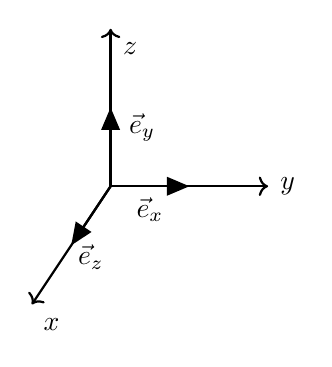
\begin{tikzpicture}
%\draw[step=0.5cm,gray,very thin] (0,0) grid (4,4); %background grid

\draw [thick,->] (1.5,2) -- (3.5,2);
\draw [thick,->] (1.5,2) -- (1.5,4);
\draw [thick,->] (1.5,2) -- (0.5,0.5);

\node[] at (0.75,0.25) {$x$};
\node[] at (3.75,2) {$y$};
\node[] at (1.75,3.75) {$z$};

\draw[>=triangle 45, line width=0.3mm, ->] (1.5,2) -- (2.5,2) ;   
\node[] at (2,1.7) {$\vec{e}_x$};

\draw[>=triangle 45, line width=0.3mm, ->] (1.5,2) -- (1.5,3) ;   
\node[] at (1.9,2.75) {$\vec{e}_y$};

\draw[>=triangle 45, line width=0.3mm, ->] (1.5,2) -- (1,1.25) ;   
\node[] at (1.25,1.1) {$\vec{e}_z$};

\end{tikzpicture}
\end{center}


\noindent Any vector can then be written
\[
{\vec V}  = V_x {\vec e}_x  + V_y {\vec e}_y + V_z \vec{e}_z
\]
The gradient of a function $f$ is 
\[
\vec{\nabla} f= \text{grad }f= 
\frac{\partial f}{\partial x}\; \vec{e}_x +
\frac{\partial f}{\partial y}\; \vec{e}_y +
\frac{\partial f}{\partial z}\; \vec{e}_z,
\]
the divergence of a vector $\vec{V}$ is
\[
\vec{\nabla}\cdot \vec{V} = 
\frac{\partial V_x}{\partial x}+
\frac{\partial V_y}{\partial y}+
\frac{\partial V_z}{\partial z}
\]
and the Laplace operator of a function $f$ is:
\[
\Delta f = 
\frac{\partial^2 f}{\partial x^2} + 
\frac{\partial^2 f}{\partial y^2} + 
\frac{\partial^2 f}{\partial z^2}  
\]
Finally the path increment is
\[
d\vec{r} = dx \; {\vec e}_x  + dy\; {\vec e}_y + dz \; \vec{e}_z
\]
and the volume element is 
\[
dV=dx\; dy \; dz
\]

%........................................
\subsubsection{Polar coordinates}

We have $r>0$ and $\theta=[0,2\pi[$, defined in the $(x,y)-$plane.

\begin{flushright} {\tiny {\color{gray} (tikz\_polar\_coordinates.tex)}} \end{flushright}
%~~~~~~~~~~~~~~~~~~~~~~~~~~~~~~~~~~~~~~~~~~~~~~~~~~~~~~~~~~~~~~~~~~~~~~~~~~~~~~~~~~~~~~~~~~~~~~~~~~
\begin{center}
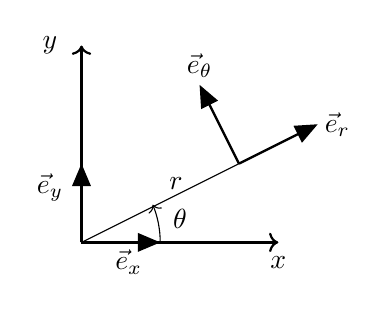
\begin{tikzpicture}
%\draw[step=0.5cm,gray,very thin] (0,0) grid (4.5,4); %background grid

\draw [thick,->] (1,1) -- (3.5,1);
\draw [thick,->] (1,1) -- (1,3.5);

\node[] at (3.5,0.75) {$x$};
\node[] at (0.6,3.5) {$y$};

\draw[>=triangle 45, line width=0.3mm, ->] (1,1) -- (2,1) ;   
\node[] at (1.6,0.75) {$\vec{e}_x$};

\draw[>=triangle 45, line width=0.3mm, ->] (1,1) -- (1,2) ;   
\node[] at (0.6,1.7) {$\vec{e}_y$};

\draw [-] (1,1) -- (3,2);

\draw[>=triangle 45, line width=0.3mm, ->] (3,2) -- (4,2.5) ;   
\node[] at (4.25,2.5) {$\vec{e}_r$};

\draw[>=triangle 45, line width=0.3mm, ->] (3,2) -- (2.5,3) ;   
\node[] at (2.5,3.25) {$\vec{e}_\theta$};


\node[] at (2.2,1.75) {$r$};
\node[] at (2.25,1.3) {$\theta$};

\draw[->] (2,1) arc (0:22.5:1.25);

\end{tikzpicture}
\end{center}


\noindent The relation between the unit vector in Cartesian and Polar/Cylindrical coordinates
is given by:
\[
\left(
\begin{array}{c}
{\vec e}_{r} \\
{\vec e}_{\theta} \\
\end{array}
\right)
=
\left(
\begin{array}{cc}
\cos \theta & \sin \theta \\
-\sin \theta & \cos \theta
\end{array}
\right)
\cdot
\left(
\begin{array}{c}
{\vec e}_{x} \\
{\vec e}_{y} \\
\end{array}
\right)
\]
which should be read:
\begin{eqnarray}
{\vec e}_{r}      &=& \cos\theta \; {\vec e}_{x} + \sin\theta \;  {\vec e}_{y} \nn\\
{\vec e}_{\theta} &=& -\sin\theta \; {\vec e}_{x} + \cos\theta \;  {\vec e}_{y} 
\end{eqnarray}
Note that this $2\times 2$ matrix is a 
rotation matrix\footnote{\url{https://en.wikipedia.org/wiki/Rotation_matrix}}
corresponding to an angle $-\theta$. The inverse of this matrix always exists 
(we can always counter-rotate) and it then yields
\[
\left(
\begin{array}{c}
{\vec e}_{x} \\
{\vec e}_{y} \\
\end{array}
\right)
=
\left(
\begin{array}{cc}
\cos \theta & -\sin \theta \\
\sin \theta & \cos \theta
\end{array}
\right)
\cdot
\left(
\begin{array}{c}
{\vec e}_{r} \\
{\vec e}_{\theta} \\
\end{array}
\right)
\]
so that for any vector ${\vec V}$
\begin{eqnarray}
{\vec V} 
&=& V_x {\vec e}_x  + V_y {\vec e}_y \nonumber\\
&=& V_x [(\cos \theta) {\vec e}_r - (\sin \theta) {\vec e}_\theta]  + 
    V_y [(\sin \theta) {\vec e}_r + (\cos \theta){\vec e}_\theta] \nonumber\\
&=& [V_x (\cos \theta) + V_y (\sin \theta)] {\vec e}_r +
[- V_x(\sin \theta) + V_y (\cos \theta)]{\vec e}_\theta \nn\\
&=& V_r \vec{e}_r  + V_\theta \vec{e}_\theta \nn
\end{eqnarray}
with
\begin{eqnarray}
V_r &=& V_x \cos \theta + V_y \sin \theta \nn\\
V_\theta &=& - V_x \sin \theta + V_y \cos \theta \nn
\end{eqnarray}
Finally the path increment is
\[
d\vec{r} = dr \; {\vec e}_r  + r \sin\theta d\theta \; {\vec e}_\theta
\]
and the volume element is 
\[
dV= r dr \; d\theta
\]

The gradient, divergence and Laplacian formulae are given in the following section.

\index{general}{Path Increment in Polar Coordinates}

%...........................................................
\subsubsection{Cylindrical coordinates \label{ss:cylcoord}}

%Redo with tikz
\begin{center}
\includegraphics[width=4cm]{images/cylindrical}\\
{\captionfont Cylindrical coordinates}
%https://tutorial.math.lamar.edu/classes/calcii/CylindricalCoords.aspx 
\end{center}

\[
{\vec V} 
= V_r \; \vec{e}_r  + V_\theta \; \vec{e}_\theta + V_z \; \vec{e}_z
\]
We have 
\begin{eqnarray}
x &=& r \; \cos\theta \nn\\
y &=& r \; \sin \theta \nn\\\ 
r &=& \sqrt{x^2+y^2} \nn
\end{eqnarray}

Let $f(r,\theta)$ be a function of the spatial coordinates. It s gradient is then
\[
\vec \nabla f
= \frac{\partial f}{\partial r} \; \vec{e}_r 
+ \frac{1}{r} \frac{\partial f}{\partial \theta} \; \vec{e}_\theta
+ \frac{\partial f}{\partial r} \; \vec{e}_z
\]
The divergence of a vector field $\vec{V}$ is 
\[
\vec\nabla \cdot \vec{V} 
= \frac{1}{r} \frac{\partial }{\partial r} (r V_r) 
+ \frac{1}{r} \frac{\partial V_\theta}{\partial \theta} 
+ \frac{\partial V_z}{\partial z}
\]
and the Laplacian of $f$ is
\[
\Delta f = \frac{1}{r} \frac{\partial }{\partial r} \left( r \frac{\partial f}{\partial r} \right)
+ \frac{1}{r^2} \frac{\partial^2 f}{\partial \theta^2} 
+ \frac{\partial^2 f}{\partial z^2} 
\]
Finally the path increment is
\[
d\vec{r} = dr \; {\vec e}_r  + r \sin\theta d\theta \; {\vec e}_\theta + dz \; \vec{e}_z
\]
and the volume element is 
\[
dV= r dr \; d\theta \; dz
\]
\index{general}{Gradient Operator in Cylindrical Coordinates}
\index{general}{Divergence Operator in Cylindrical Coordinates}
\index{general}{Laplace Operator in Cylindrical Coordinates}
\index{general}{Path Increment in Cylindrical Coordinates}

\begin{remark} 
Cylindrical coordinates can also be denoted by $(\rho,\theta)$, $(r,\phi)$ or even $(\rho,\phi)$.
They are sometimes called "cylindrical polar coordinates" or "polar cylindrical coordinates".
\end{remark}

%........................................
\subsubsection{Spherical coordinates \label{ss:sphercoord}}

On the following figure are represented the three Cartesian axis, 
a point and its spherical coordinates $r,\theta,\phi$:
\begin{center}
\includegraphics[width=5cm]{images/sphcoord}\\
{\captionfont Spherical coordinates as commonly used in physics:\\ polar angle $\theta$, and azimuthal angle $\phi$.} 
\end{center}
In this case $\theta\in[0:\pi]$ and $\phi\in]-\pi:\pi]$ and we have the following relationships:
\begin{eqnarray}
r &=& \sqrt{x^2+y^2+z^2} \\
\theta &=& \arccos (z/r) \\
\phi &=& \arctan (y/x) \\
x &=& r \sin \theta \cos \phi \\
y &=& r \sin\theta \sin\phi \\
z &=& r \cos\theta 
\end{eqnarray}
The inverse tangent used to compute $\phi$ must be suitably defined, 
taking into account the correct quadrant of $(x,y)$,
which is why the atan2 intrinsic function is used in \textsc{FORTRAN} for example.    
This is often written as follows:
\begin{eqnarray}
\theta &=& \arctan \left(\sqrt{x^2+y^2},z\right) \\
\phi &=& \arctan (y,x) 
\end{eqnarray}
where we formally take advantage of the two argument arctan
function to eliminate quadrant confusion.

The path increment is expressed as:

\begin{equation}
d\vec{r} = dr \; \vec{e}_r + r d\theta \; \vec{e}_\theta + r \sin\theta d\phi \; \vec{e}_\phi
\end{equation}
The gradient of a function $f(r,\theta,\phi)$ is 
\begin{equation}
\vec\nabla f= \frac{\partial f}{\partial r} \; \vec{e}_r
+ \frac{1}{r} \frac{\partial f}{\partial \theta} \; \vec{e}_\theta 
+ \frac{1}{r \; \sin\theta} \frac{\partial f}{\partial \phi} \;  \vec{e}_\phi
\end{equation}
The divergence of a vector $\vec{V}$ is
\begin{equation}
\vec\nabla\cdot \vec{V}=
\frac{1}{r^2} \frac{\partial}{\partial r} \left(r^2 V_r \right) 
+
\frac{1}{r \sin\theta} \frac{\partial}{\partial \theta} (V_\theta \sin\theta)
+
\frac{1}{r \sin\theta} \frac{\partial V_\phi}{\partial \phi}=0
\label{eq:divsc}
\end{equation}
The Laplacian of function $f$ is given by: \index{general}{Laplacian}
\begin{equation}
\Delta f= \vec\nabla \cdot\vec\nabla f= \vec\nabla^2 f
=
\frac{1}{r^2}\frac{\partial}{\partial r} \left( r^2 \frac{\partial f}{\partial r} \right)
+\frac{1}{r^2 \sin\theta} \frac{\partial}{\partial \theta} \left( \sin\theta \frac{\partial f}{\partial \theta} \right)
+\frac{1}{r^2 \sin^2\theta}  \frac{\partial^2 f}{\partial \phi^2}
\end{equation}

In geography one uses latitude and longitude, represented hereunder:
\begin{center}
\includegraphics[width=10cm]{images/map.jpg}
\end{center}
\begin{itemize}
\item Latitude  $\in[-90:90]$,   or $\in[-\pi/2:\pi/2]$ 
\item Longitude $\in]-180:180]$, or $\in]-\pi:\pi]$ 
\end{itemize}

Since the colatitude is the complementary angle of the latitude, 
i.e. the difference between 90 and the latitude, 
where southern latitudes are denoted with a minus sign,
$\theta$ as shown above is actually is the colatitude.
The colatitude is shown in red on the following figure: 
\index{general}{Colatitude}
\begin{center}
\includegraphics[width=3cm]{images/colatitude}
\end{center}

The volume of a sphere of radius $R$ is easily obtained by computing 
\begin{eqnarray}
V_{sphere} 
&=& \iiint_{sphere} dV \nn\\
&=& \int_0^R r^2 dr \int_0^\pi \sin\theta d\theta \int_0^{2\pi} d\phi  \nn\\
&=& \frac{1}{3}R^3  \cdot 2 \cdot 2\pi \nn\\
&=& \frac{4}{3}\pi R^3 
\end{eqnarray}
\index{general}{Volume of a Sphere}

The volume of a spherical shell of inner radius $R_i$ and outer radius $R_o$
is equally easily obtained by computing 

\begin{eqnarray}
V_{shell}
&=& \iiint_{shell} dV \nn\\
&=& \int_{R_i}^{R_o} r^2 dr \int_0^\pi \sin\theta d\theta \int_0^{2\pi} d\phi  \nn\\
&=& \frac{1}{3}(R_o^3-R_i^3)  \cdot 2 \cdot 2\pi \nn\\
&=& \frac{4}{3}\pi (R^3_o -R^3_i)
\end{eqnarray}
\index{general}{Volume of a Spherical shell}


\noindent The spherical unit vectors are related to the Cartesian unit vectors by:
\[
\left(
\begin{array}{c}
\vec{e}_{r} \\ \vec{e}_\theta \\ \vec{e}_\phi
\end{array}
\right)
=
\left(
\begin{array}{ccc}
\sin\theta \cos\phi & \sin\theta\sin\phi & \cos\theta  \\
\cos\theta \cos\phi & \cos\theta\sin\phi & -\sin\theta \\
-\sin\phi & \cos\phi & 0
\end{array}
\right)
\left(
\begin{array}{c}
\vec{e}_{x} \\ \vec{e}_y \\ \vec{e}_z
\end{array}
\right)
\]
and the Cartesian unit vectors are related to the spherical unit vectors by

\[
\left(
\begin{array}{c}
\vec{e}_{x} \\ \vec{e}_y \\ \vec{e}_z
\end{array}
\right)
=
\left(
\begin{array}{ccc}
\sin\theta \cos\phi & \cos\theta\cos\phi & -\sin\phi  \\
\sin\theta \sin\phi & \cos\theta\sin\phi & \cos\phi \\
\cos\theta & -\sin\theta & 0
\end{array}
\right)
\left(
\begin{array}{c}
\vec{e}_{r} \\ \vec{e}_\theta \\ \vec{e}_\phi
\end{array}
\right)
\]

\begin{eqnarray}
\vec{\upnu} 
&=& u\; \vec{e}_x + v \; \vec{e}_y + w \; \vec{e}_z \\
&=& u\; ( \sin\theta \cos\phi \; \vec{e}_r +  \cos\theta\cos\phi \;  \vec{e}_{\theta} -\sin\phi \; \vec{e}_{\phi} ) \\
&+& v\; ( \sin\theta \sin\phi \; \vec{e}_r + \cos\theta\sin\phi \; \vec{e}_\theta  +  \cos\phi \;  \vec{e}_\phi  )  \\
&+& w\; ( \cos\theta \; \vec{e}_r   -\sin\theta \; \vec{e}_\theta  ) \\
&=& v_r\; \vec{e}_r + v_\theta\; \vec{e}_\theta + v_\phi\; \vec{e}_\phi 
\end{eqnarray}
with 
\begin{eqnarray}
v_r      &=&  u \sin \theta  \cos \phi  + v \sin\theta \sin \phi + w \cos\theta \\
v_\theta &=&  u \cos\theta\cos\phi + v \cos\theta\sin\phi -w \sin\theta   \\
v_\phi   &=& -u \sin\phi  + v \cos\phi  
\end{eqnarray}

%.................................................................................................
\subsubsection{Converting tensors between Cartesian and Cylindrical bases \label{ss:convcartspher}}

\[
{\bm T}_{\tiny Cyl}=
\left(
\begin{array}{ccc}
T_{rr}       & T_{r\theta}      & T_{rz} \\
T_{\theta r} & T_{\theta\theta} & T_{\theta z} \\
T_{z r}      & T_{z \theta}     & T_{zz}
\end{array}
\right)
=
\left(
\begin{array}{ccc}
 \cos \theta&\sin \theta&0 \\
-\sin \theta&\cos \theta&0 \\
0 & 0 & 1 
\end{array}
\right)
\cdot
\left(
\begin{array}{ccc}
T_{xx} & T_{xy} & T_{xz} \\
T_{yx} & T_{yy} & T_{yz} \\
T_{zx} & T_{zy} & T_{zz} 
\end{array}
\right)
\cdot
\left(
\begin{array}{ccc}
\cos \theta & -\sin \theta&0 \\
\sin \theta &  \cos \theta&0 \\
0 & 0 & 1 
\end{array}
\right)
\]

\[
{\bm T}_{\tiny Cart}=
\left(
\begin{array}{ccc}
T_{xx} & T_{xy} & T_{xz} \\
T_{yx} & T_{yy} & T_{yz} \\
T_{zx} & T_{zy} & T_{zz} 
\end{array}
\right)
=
\left(
\begin{array}{ccc}
 \cos \theta&-\sin \theta&0 \\
\sin \theta&\cos \theta&0 \\
0 & 0 & 1 
\end{array}
\right)
\cdot
\left(
\begin{array}{ccc}
T_{rr}       & T_{r\theta}      & T_{rz} \\
T_{\theta r} & T_{\theta\theta} & T_{\theta z} \\
T_{z r}      & T_{z \theta}     & T_{zz}
\end{array}
\right)
\cdot
\left(
\begin{array}{ccc}
\cos \theta & \sin \theta&0 \\
-\sin \theta &  \cos \theta&0 \\
0 & 0 & 1 
\end{array}
\right)
\]



%.................................................................................................
\subsubsection{Converting tensors between Cartesian and Spherical bases \label{ss:convcartspher}}

Let ${\bm T}$ be a tensor
\[
{\bm T}=
\left(
\begin{array}{ccc}
T_{xx} & T_{xy} & T_{xz} \\
T_{yx} & T_{yy} & T_{yz} \\
T_{zx} & T_{zy} & T_{zz} 
\end{array}
\right)
\qquad\qquad
{\bm T}=
\left(
\begin{array}{ccc}
T_{rr}       & T_{r\theta}      & T_{r\phi} \\
T_{\theta r} & T_{\theta\theta} & T_{\theta\phi} \\
T_{\phi r}   & T_{\phi \theta}  & T_{\phi\phi}
\end{array}
\right)
\]
in the Cartesian basis (left) and the spherical basis (right).

The two sets of components are related by
\[
\left(
\begin{array}{ccc}
T_{xx} & T_{xy} & T_{xz} \\
T_{yx} & T_{yy} & T_{yz} \\
T_{zx} & T_{zy} & T_{zz} 
\end{array}
\right)
=
\left(
\begin{array}{ccc}
\sin\theta \; \cos\phi & \cos\theta \; \cos\phi & -\sin\phi \\
\sin\theta \; \sin\phi & \cos\theta \; \sin\phi &  \cos\phi \\
\cos\theta & -\sin\theta & 0 
\end{array}
\right)
\cdot
\left(
\begin{array}{ccc}
T_{rr}       & T_{r\theta}      & T_{r\phi} \\
T_{\theta r} & T_{\theta\theta} & T_{\theta\phi} \\
T_{\phi r}   & T_{\phi \theta}  & T_{\phi\phi}
\end{array}
\right)
\cdot
\left(
\begin{array}{ccc}
\sin\theta\;\cos\phi & \sin\theta\;\sin\phi & \cos\theta \\
\cos\theta\;\cos\phi & \cos\theta\;\sin\phi & -\sin\theta \\
-\sin\phi & \cos\phi & 0 
\end{array}
\right)
\]
or
\[
\left(
\begin{array}{ccc}
T_{rr}       & T_{r\theta}      & T_{r\phi} \\
T_{\theta r} & T_{\theta\theta} & T_{\theta\phi} \\
T_{\phi r}   & T_{\phi \theta}  & T_{\phi\phi}
\end{array}
\right)
=
\left(
\begin{array}{ccc}
\sin\theta \; \cos\phi & \sin\theta \; \sin\phi & \cos\theta \\
\cos\theta \; \cos\phi & \cos\theta \; \sin\phi & -\sin\theta \\
-\sin\phi & \cos\phi & 0 
\end{array}
\right)
\cdot
\left(
\begin{array}{ccc}
T_{xx} & T_{xy} & T_{xz} \\
T_{yx} & T_{yy} & T_{yz} \\
T_{zx} & T_{zy} & T_{zz} 
\end{array}
\right)
\cdot
\left(
\begin{array}{ccc}
\sin\theta\;\cos\phi & \cos\theta\;\cos\phi & -\sin\phi \\
\sin\theta\;\sin\phi & \cos\theta\;\sin\phi & \cos\phi \\
\cos\theta & -\sin\theta & 0
\end{array}
\right)
\]
If we now assume that the tensor ${\bm T}$ is symmetric (e.g. stress tensor, strain rate tensor),
then there are only 6 independent terms.

 \label{ss:coordsys} %-------------------
\newpage
\section{A continuum mechanics primer} %--------------------------------------------------------
\begin{flushright} {\tiny {\color{gray} continuum\_mechanics.tex}} \end{flushright}
%~~~~~~~~~~~~~~~~~~~~~~~~~~~~~~~~~~~~~~~~~~~~~~~~~~~~~~~~~~~~~~~~~~~~~~~~~~~~~~~~~~~~~~~~~~~~~~~~~~

{\sl Contains contributions by W. Spakman} \index{contributors}{W. Spakman}

%......................................................................
\subsubsection{Forces}

In continuum mechanics we make a distinction between two broad classes of forces:
\begin{itemize}
\item Body forces defined as force per unit volume (N/m$^3$): gravity, electro-magnetic forces
\item Tractions: Surface forces defined as force per unit surface area (N/m$^2$):
Contact forces, elastic forces per unit area, internal flow friction, pressure, ...\\
A traction is the surface average of all atomic forces exerted by
atoms on the one side on atoms on the other side of the surface.
For real-Earth processes, internal tractions are ultimately caused by
the body forces, usually gravity.


Existing mantle flow(i.e. flow that is forced elsewhere) can exert
tractions (shear stresses) on the subducting slab or for instance at
the base of lithosphere plates.
In HPT-laboratory experiments external tractions (pressure, shear
traction) are applied to a rock sample, which cause internal
tractions to balance the exerted forces.

\begin{center}
\includegraphics[width=6cm]{images/contmech/spak1}
\end{center}
\end{itemize}

%......................................................................
\subsubsection{Stress tensor and tractions}\label{sec:stresstensor}
\index{general}{Stress Tensor} 
\index{general}{Normal Stress} 
\index{general}{Shear Stress} 
\index{general}{Stress Vector} 
\index{general}{Traction}

The Cauchy tensor\footnote{\url{https://en.wikipedia.org/wiki/Cauchy_stress_tensor}} 
consists of nine components $\sigma_{ij}$  that completely define the state of stress 
at a point inside a material. 
The tensor relates a unit-length direction vector $\vec{n}$ to the so-called 'stress vector' (most commonly called 'traction') $\vec{t}(\vec{n})$ across an imaginary surface perpendicular to $\vec{n}$:
\[
\vec{t}(\vec n)= {\vec n} \cdot {\bm \sigma}
\]

\begin{center}
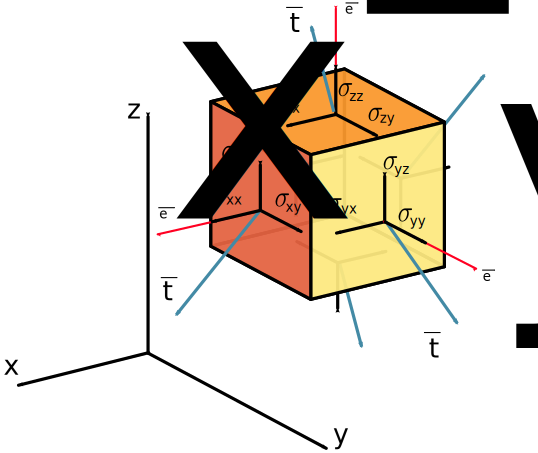
\includegraphics[width=7cm]{images/contmech/Components_stress_tensor_cartesian}\\
{\scriptsize Modified from original 
file on Wikipedia\footnote{\url{https://commons.wikimedia.org/wiki/File:Components_stress_tensor_cartesian.svg}}}
\end{center}

With respect to an orthonormal basis $\{\vec{e}_x,\vec{e}_y,\vec{e}_z\}$, the Cauchy stress tensor
is given by:
\begin{equation}
{\bm \sigma}=
\left(
\begin{array}{ccc}
\sigma_{xx} & \sigma_{xy} & \sigma_{xz} \\
\sigma_{yx} & \sigma_{yy} & \sigma_{yz} \\
\sigma_{zx} & \sigma_{zy} & \sigma_{zz} 
\end{array}
\right)
\end{equation}
The three diagonal elements are called normal stresses while the off-diagonal terms 
are called shear stresses.

One can easily prove (see for instance Section 3.3.6 of \cite{grbl09}) that the balance 
of angular momentum leads reduces to the statement that the Cauchy stress tensor 
is symmetric, i.e. ${\bm \sigma}={\bm \sigma}^T$.
Therefore, the stress state of the medium at any point and instant can be specified by only six independent parameters, rather than nine:
\begin{equation}
{\bm \sigma}=
\left(
\begin{array}{ccc}
\sigma_{xx} & \sigma_{xy} & \sigma_{xz} \\
\sigma_{xy} & \sigma_{yy} & \sigma_{yz} \\
\sigma_{xz} & \sigma_{yz} & \sigma_{zz} 
\end{array}
\right)
\qquad\qquad
\text{or sometimes}
\qquad\qquad
{\bm \sigma}=
\left(
\begin{array}{ccc}
\sigma_{x}  & \tau_{xy}  & \tau_{xz} \\
\tau_{xy}   & \sigma_{y} & \tau_{yz} \\
\tau_{xz}   & \tau_{yz}  & \sigma_{z} 
\end{array}
\right)
\end{equation}
where the elements $\sigma _{x}$, $\sigma _{y}$, $\sigma _{z}$ are called the orthogonal 
normal stresses (relative to the chosen coordinate system), and $\tau _{xy}$, $\tau _{xz}$,
$\tau _{yz}$ the orthogonal shear stresses.
As seen above, the SI units of both stress tensor and traction are \si{\newton\per\square\metre}.

In Cylindrical coordinates the stress tensor components are given by:
\begin{eqnarray}
\sigma_{rr} &=& -p + 2 \eta \frac{\partial \upnu_r}{\partial r}      \\
\sigma_{\theta\theta} &=& 
 -p + 2\eta \left( \frac{1}{r} \frac{\partial \upnu_\theta}{\partial\theta} +\frac{\upnu_r}{r} \right)    \\
\sigma_{zz} &=& -p + 2 \eta \frac{\partial \upnu_z}{\partial z}      \\
\sigma_{r\theta} &=& \eta \left( \frac{1}{r} \frac{\partial \upnu_r}{\partial \theta} 
+ \frac{\partial \upnu_\theta}{\partial r} - \frac{\upnu_\theta}{r} \right)  \\
\sigma_{rz} &=& \eta \left( \frac{\partial \upnu_r}{\partial z}  + \frac{\partial \upnu_z}{\partial r}\right) \\
\sigma_{\theta z} &=&  \eta \left(  \frac{1}{r} \frac{\partial \upnu_z}{\partial \theta}
+\frac{\partial \upnu_\theta}{\partial z}     \right) 
\end{eqnarray}
\index{general}{Stress Tensor (Cylindrical Coordinates)}

In Spherical coordinates the stress tensor components are given by:
\begin{eqnarray}
\sigma_{rr} &=& -p + 2 \eta \frac{\partial \upnu_r}{\partial r}      \\
\sigma_{\theta\theta} &=& 
 -p + 2\eta \left( \frac{1}{r} \frac{\partial \upnu_\theta}{\partial\theta} +\frac{\upnu_r}{r} \right)    \\
\sigma_{\phi\phi} &=& 
-p + 2\eta \left( \frac{1}{r \sin \theta} \frac{\partial \upnu_\phi}{\partial \phi} 
+\frac{\upnu_r}{r}  + \frac{\upnu_\theta \cot \theta}{r} \right) \\
\sigma_{r\theta} &=& \eta\left(  r \frac{\partial}{\partial r} \frac{\upnu_\theta}{r}  
+\frac{1}{r} \frac{\partial \upnu_r}{\partial\theta}   \right)\\
\sigma_{r\phi} &=& \eta \left( \frac{1}{r \sin\theta}\frac{\partial \upnu_r}{\partial \phi} 
+ r \frac{\partial}{\partial r} \frac{\upnu_\phi}{r}  \right)\\
\sigma_{\theta \phi} &=& \eta \left(
\frac{1}{r \sin\theta} \frac{\partial \upnu_\theta}{\partial\phi}
+\frac{\sin\theta}{r} \frac{\partial}{\partial \theta} \frac{\upnu_\phi}{\sin\theta}
\right) 
\end{eqnarray}
\index{general}{Stress Tensor (Spherical Coordinates)}

 %----------------------------------------------------------------------

\begin{center}
\begin{tabular}{lll}
\hline
Symbol & meaning & unit \\
\hline
\hline
$t$ & Time & s \\
$x,y,z$ & Cartesian coordinates & m \\
${\bm v}$ & velocity vector & m$\cdot$ s$^{-1}$\\
$\rho$ & mass density & kg/m$^3$ \\
$\eta$ & dynamic viscosity &  Pa$\cdot$ s \\
$\lambda$ & penalty parameter & Pa$\cdot$ s \\
$T$ & temperature & K \\
${\bm \nabla}$ & gradient operator & m$^{-1}$ \\
${\bm \nabla}\cdot$ & divergence operator & m$^{-1}$ \\
$p$ & pressure & Pa\\
$\dot{\bm \varepsilon}({\bm v})$ & strain rate tensor & s$^{-1}$ \\
$\alpha$ & thermal expansion coefficient & K$^{-1}$ \\
$k$ & thermal conductivity & W/(m $\cdot$ K) \\
$C_p$ & Heat capacity & J/K \\
$H$ & intrinsic specific heat production & W/kg\\
$\beta_T$ & isothermal compressibility & Pa$^{-1}$  \\
${\bm \tau}$ & deviatoric stress tensor & Pa \\
${\bm \sigma}$ & full stress tensor & Pa \\
\hline
\end{tabular}
\end{center}

%------------------------------------------------------------------------
\subsection{The heat transport equation - energy conservation equation}

Let us start from the heat transport equation as shown in Schubert, Turcotte and Olson \cite{scto01}:
\[
\rho C_p \frac{DT}{Dt} - \alpha T \frac{Dp}{Dt} = {\bm \nabla} \cdot k {\bm \nabla} T + \Phi + \rho H  
\]
with $D/Dt$ being the total derivatives so that 
\[
\frac{DT}{Dt} = \frac{\partial T}{\partial t} + {\bm v}\cdot {\bm \nabla}T
\quad\quad
\frac{Dp}{Dt} = \frac{\partial p}{\partial t} + {\bm v}\cdot {\bm \nabla}p
\]
Solving for temperature, this equation is often rewritten as follows:
\begin{mdframed}[backgroundcolor=blue!5]
\[
\rho C_p \frac{DT}{Dt} - {\bm \nabla} \cdot k {\bm \nabla} T =  \alpha T \frac{Dp}{Dt} + \Phi + \rho H  
\]
\end{mdframed}

A note on the shear heating term $\Phi$: In many publications, $\Phi$ 
is given by $\Phi=\tau_{ij}\partial_j u_i={\bm \tau}:{\bm \nabla}{\bm v}$.

\begin{eqnarray}
\Phi 
&=& \tau_{ij}\partial_j u_i \nonumber\\
&=& 2 \eta \dot{\varepsilon}_{ij}^d\partial_j u_i \nonumber\\
&=& 2 \eta \frac{1}{2}\left( \dot{\varepsilon}_{ij}^d\partial_j u_i + \dot{\varepsilon}_{ji}^d\partial_i u_j \right) \nonumber\\
&=& 2 \eta \frac{1}{2}\left( \dot{\varepsilon}_{ij}^d\partial_j u_i + \dot{\varepsilon}_{ij}^d\partial_i u_j \right) \nonumber\\
&=& 2 \eta  \dot{\varepsilon}_{ij}^d  \frac{1}{2}\left(\partial_j u_i + \partial_i u_j \right) \nonumber\\
&=& 2 \eta  \dot{\varepsilon}_{ij}^d   \dot{\varepsilon}_{ij} \nonumber\\
&=& 2 \eta  \dot{\bm \varepsilon}^d :  \dot{\bm \varepsilon} \nonumber\\
&=& 2 \eta  \dot{\bm \varepsilon}^d : \left( \dot{\bm \varepsilon}^d +\frac{1}{3} ({\bm \nabla}\cdot{\bm v}) {\bm 1} \right)\nonumber\\
&=& 2 \eta  \dot{\bm \varepsilon}^d : \dot{\bm \varepsilon}^d 
+ 2 \eta  \dot{\bm \varepsilon}^d : {\bm 1} ({\bm \nabla}\cdot{\bm v}) \nonumber\\ 
&=& 2 \eta  \dot{\bm \varepsilon}^d : \dot{\bm \varepsilon}^d 
\end{eqnarray}
Finally
\[
\Phi = {\bm \tau}:{\bm \nabla}{\bm v} = 2 \eta  \dot{\bm \varepsilon}^d : \dot{\bm \varepsilon}^d
= 2 \eta \left( (\dot{\varepsilon}_{xx}^d)^2 + (\dot{\varepsilon}_{yy}^d)^2 + 2(\dot{\varepsilon}_{xy}^d)^2 \right)
\]

%------------------------------------------------------------------------
\subsection{The momentum conservation equations} 

Because the Prandlt number is virtually zero in Earth science applications the Navier Stokes 
equations reduce to the Stokes equation:
\[
{\bm \nabla}\cdot {\bm \sigma} + \rho {\bm g} = 0
\]
Since 
\[
{\bm \sigma} = -p {\bm 1} + {\bm \tau}
\]
it also writes
\[
-{\bm \nabla}p + {\bm \nabla}\cdot {\bm \tau} + \rho {\bm g} = 0
\]
Using the relationship ${\bm \tau} = 2 \eta \dot{\bm \varepsilon}^d$ we arrive at 
\begin{mdframed}[backgroundcolor=blue!5]
\[
-{\bm \nabla}p + {\bm \nabla}\cdot (2 \eta \dot{\bm \varepsilon}^d ) + \rho {\bm g} = 0
\]
\end{mdframed}

%------------------------------------------------------------------------
\subsection{The mass conservation equations} 

The mass conservation equation is given by
\[
\frac{D\rho}{Dt} + \rho {\bm \nabla}\cdot{\bm v} = 0
\]
or, 
\begin{mdframed}[backgroundcolor=blue!5]
\[
\frac{\partial \rho}{\partial t} + {\bm \nabla}\cdot(\rho {\bm v}) = 0
\]
\end{mdframed}
In the case of an incompressible flow, then $\partial \rho/\partial t=0$ and 
${\bm \nabla}\rho=0$, i.e. $D\rho/Dt=0$ and the remaining equation is simply:
\[
{\bm \nabla}\cdot{\bm v} = 0
\]

\subsection{The equations in ASPECT manual}
The following is lifted off the ASPECT manual.
We focus on the system of equations in a $d=2$- or $d=3$-dimensional
domain $\Omega$ that describes the motion of a highly viscous fluid driven
by differences in the gravitational force due to a density that depends on
the temperature. In the following, we largely follow the exposition of this
material in Schubert, Turcotte and Olson \cite{scto01}.

Specifically, we consider the following set of equations for velocity $\mathbf
u$, pressure $p$ and temperature $T$:
\begin{align}
  \label{eq:stokes-1}
  -\nabla \cdot \left[2\eta \left(\dot\varepsilon(\bm v)
                                  - \frac{1}{3}(\nabla \cdot \bm v)\mathbf 1\right)
                \right] + \nabla p &=
  \rho \bm g
  &
  & \textrm{in $\Omega$},
  \\
  \label{eq:stokes-2}
  \nabla \cdot (\rho \bm v) &= 0
  &
  & \textrm{in $\Omega$},
  \\
  \label{eq:temperature}
  \rho C_p \left(\frac{\partial T}{\partial t} + \bm v\cdot\nabla T\right)
  - \nabla\cdot k\nabla T
  &=
  \rho H
  \notag
  \\
  &\quad
  +
  2\eta
  \left(\dot\varepsilon(\bm v) - \frac{1}{3}(\nabla \cdot \bm v)\mathbf 1\right)
  :
  \left(\dot\varepsilon(\bm v) - \frac{1}{3}(\nabla \cdot \bm v)\mathbf 1\right)
  \\
  &\quad
  +\alpha T \left( \bm v \cdot \nabla p \right)
  \notag
  \\
  &\quad
  &
  & \textrm{in $\Omega$},
  \notag
\end{align}
where $\dot{\bm \varepsilon}(\mathbf u) = \frac{1}{2}(\nabla \mathbf u + \nabla\mathbf
u^T)$ is the symmetric gradient of the velocity (often called the
\textit{strain rate}).%

In this set of equations, \eqref{eq:stokes-1} and \eqref{eq:stokes-2}
represent the compressible Stokes equations in which $\mathbf v=\mathbf
v(\mathbf x,t)$ is the velocity field and $p=p(\mathbf x,t)$ the pressure
field. Both fields depend on space $\mathbf x$ and time $t$. Fluid flow is
driven by the gravity force that acts on the fluid and that is proportional to
both the density of the fluid and the strength of the gravitational pull.

Coupled to this Stokes system is equation \eqref{eq:temperature} for the
temperature field $T=T(\mathbf x,t)$ that contains heat conduction terms as
well as advection with the flow velocity $\mathbf v$. The right hand side
terms of this equation correspond to
\begin{itemize}
\item internal heat production for example due to radioactive decay;
\item friction (shear) heating;
\item adiabatic compression of material;
\end{itemize}

In order to arrive at the set of equations that ASPECT solves, 
we need to 
\begin{itemize}
\item neglect the $\partial p/\partial t$. {\color{red}WHY?}
\item neglect the $\partial \rho / \partial t$ . {\color{red}WHY?}
\end{itemize}
from equations above. 

----------------------------------------

Also, their definition of the shear heating term $\Phi$ is:
\[
\Phi = k_B ({\bm \nabla}\cdot{\bm v})^2 + 2\eta \dot{\bm \varepsilon}^d:\dot{\bm \varepsilon}^d
\]
For many fluids the bulk viscosity $k_B$ is very small and is often taken to be zero, an assumption known
as the Stokes assumption: $k_B=\lambda+2\eta/3=0$. \index{bulk viscosity}
Note that $\eta$ is the dynamic viscosity and $\lambda$ the second viscosity. \index{dynamic viscosity}
\index{second viscosity}
Also, 
\[
{\bm \tau}=2\eta \dot{\bm \varepsilon} + \lambda ({\bm \nabla}\cdot{\bm v}) {\bm 1}
\]
but since $k_B=\lambda+2\eta/3=0$, then $\lambda=-2\eta/3$ so 
\[
{\bm \tau}=2\eta \dot{\bm \varepsilon} -\frac{2}{3}\eta ({\bm \nabla}\cdot{\bm v}) {\bm 1} = 2\eta \dot{\bm \varepsilon}^d
\]







\newpage
%---------------------------------
\subsection{the Boussinesq approximation: an Incompressible flow}

\index{Boussinesq}

[from aspect manual]
The Boussinesq approximation assumes that the density can be
considered constant in all occurrences in the equations with the exception of
the buoyancy term on the right hand side of \eqref{eq:stokes-1}. The primary
result of this assumption is that the continuity equation \eqref{eq:stokes-2}
will now read
\[
{\bm \nabla}\cdot{\bm v} = 0
\]
This implies that the strain rate tensor is deviatoric.
Under the Boussinesq approximation, the equations are much simplified:

\begin{align}
  \label{eq:stokes-1}
  -\nabla \cdot \left[2\eta \dot{\bm \varepsilon}(\bm v)
                \right] + \nabla p &=
  \rho \bm g
  &
  & \textrm{in $\Omega$},
  \\
  \label{eq:stokes-2}
  \nabla \cdot (\rho \bm v) &= 0
  &
  & \textrm{in $\Omega$},
  \\
  \label{eq:temperature}
  \rho_0 C_p \left(\frac{\partial T}{\partial t} + \bm v\cdot\nabla T\right)
  - \nabla\cdot k\nabla T
  &=
  \rho H
  &
  & \textrm{in $\Omega$}
\end{align}
Note that all terms on the rhs of the temperature equations have disappeared, with the exception 
of the source term.


\newpage
\subsection{Stokes equation for elastic medium}

What follows is mostly borrowed from Becker \& Kaus lecture notes.

%\begin{tabular}{|l|l|l|}
%\hline
%${\bm u}       $ & displacement vector &   \\
%${\bm \sigma}  $ & full stress tensor  & Pa\\
%${\bm \epsilon}$ & strain tensor       &   \\
%${\bm 1}       $ & unit tensor         &   \\
%${\bm f}       $ & body forces         &   \\
%\hline
%\end{tabular}

The strong form of the PDE that governs force balance in a medium is given by
\[
{\bm \nabla}\cdot{\bm \sigma}  + {\bm f} = {\bm 0}
\]
where ${\bm \sigma}$ is the stress tensor and ${\bm f}$ is a body force.

The stress tensor is related to the strain tensor through the generalised 
Hooke's law:
\begin{equation}
\sigma_{ij}=\sum_{kl}C_{ijkl}\epsilon{kl} \label{eq:one}
\end{equation}
where ${\bm C}$ is the fourth-order elastic tensor.
In the case of an isotropic material, this relationship simplifies to
\begin{equation}
\sigma_{ij}=\lambda \epsilon_{kk} \delta_{ij} + 2\mu \epsilon_{ij}
\quad\quad
or, 
\quad\quad
{\bm \sigma} = \lambda ({\bm \nabla}\cdot{\bm u})  {\bm 1} + 2\mu {\bm \epsilon}   \label{eq:two}
\end{equation}
where $\lambda$ is the Lam\'e parameter and $\mu$ is the shear modulus\footnote{It is also sometimes written $G$}.
The term ${\bm \nabla}\cdot{\bm u}$ is the isotropic dilation.

\index{Lam\'e parameter} \index{shear modulus}

The strain tensor is related to the displacement as follows: \index{strain tensor}
\[
{\bm \epsilon} = \frac{1}{2}({\bm \nabla}{\bm u} + {\bm \nabla}{\bm u}^T)
\]

The incompressibility (bulk modulus), $K$, is defined as $p=-K {\bm \nabla}\cdot{\bm u}$ 
where $p$ is the pressure with \index{bulk modulus}
\begin{eqnarray}
p&=&-\frac{1}{3}Tr({\bm \sigma}) \nonumber\\
 &=& -\frac{1}{3} [ \lambda ({\bm \nabla}\cdot{\bm u}) Tr[{\bm 1}] + 2 \mu Tr[{\bm \epsilon}]] \nonumber\\
 &=& -\frac{1}{3} [ \lambda ({\bm \nabla}\cdot{\bm u})  3  + 2 \mu  ({\bm \nabla}\cdot{\bm u}) ] \nonumber\\
 &=& -[ \lambda  + \frac{2}{3} \mu ]   ({\bm \nabla}\cdot{\bm u})  
\end{eqnarray}
so that $K=\lambda+\frac{2}{3}\mu$.

%or
%\[
%\mu=\frac{3K(1-2\nu)}{2(1+\nu)}
%\]


\paragraph{Remark}: Eq. (\ref{eq:one}) and (\ref{eq:two}) are analogous to the ones that one has to solve
in the context of viscous flow using the penalty method. In this case $\lambda$ is the penalty coefficient, 
${\bm u}$ is the velocity, and $\mu$ is then the dynamic viscosity.

%\begin{center}
%\includegraphics[width=15cm]{images/coeffs}\\
%{\small Homogeneous isotropic linear elastic materials have their elastic properties uniquely determined by any two moduli among these; thus, given any two, any other of the elastic moduli can be calculated according to these formulas.}
%\end{center}

The Lam\'e parameter and the shear modulus are also linked to $\nu$ the poisson ratio, 
and $E$, Young's modulus: \index{Poisson ratio} \index{Young's modulus}
\[
\lambda=\mu\frac{2\nu}{1-2\nu}
=\frac{\nu E}{(1+\nu)(1-2\nu)}
\quad\quad
{\rm with}
\quad\quad
E=2\mu(1+\nu)
\]
The shear modulus, expressed often in GPa, describes the material's response to shear stress.
The poisson ratio describes the response in the direction orthogonal to uniaxial stress.
The Young modulus, expressed in GPa, describes the material's strain response to uniaxial stress in the 
direction of this stress.









 %----------------------------------------------------------------------------------

\newpage
\section{Moment of inertia} \begin{flushright} {\tiny {\color{gray} momentofinertia.tex}} \end{flushright}

% borrowed from http://farside.ph.utexas.edu/teaching/336k/Newtonhtml/node64.html

Consider a rigid body rotating with fixed angular velocity $\omega$ about an axis which passes through the origin.
Let ${\bm r}_i$ be the position vector of the $i$th mass element, whose 
mass is $m_i$. We expect this position vector to precess about the axis of rotation (which is parallel to $\omega$) 
with angular velocity $\omega$. 

\begin{displaymath} 
\frac{d{\bm r}_i}{dt} = \mbox{\boldmath$\omega$}\times {\bm r}_i. 
\end{displaymath}

Thus, the above equation specifies the velocity, ${\bm v}_i = d{\bm r}_i/dt$, of each mass element as the body rotates with fixed angular velocity $\omega$ about an axis passing through the origin. 


The total angular momentum of the body (about the origin) is written
\begin{displaymath} 
{\bm L} 
= \sum_{i=1,N} m_i\,{\bm r}_i\times\frac{d{\bm r}_i}{dt}
= \sum_{i=1,N} m_i\,{\bm r}_i\times ( \mbox{\boldmath$\omega$}\times {\bm r}_i )
= \sum_{i=1,N} m_i\, [ r_i^2 {\bm \omega} - ({\bm r}_i\cdot {\bm \omega}) {\bm r}_i ]
\end{displaymath}
The above formula can be written as a matrix equation of the form
\begin{displaymath} 
\left(\begin{array}{c}L_x\\ L_y\\ L_z\end{array}\right)=
\left(\begin{array}{ccc}
I_{xx} & I_{xy} & I_{xz} \\
I_{yx} & I_{yy} & I_{yz} \\
I_{zx} & I_{zy} & I_{zz} 
\end{array}\right) 
\left(\begin{array}{c}\omega_x\\ \omega_y\\ \omega_z\end{array}\right)
\end{displaymath}
where

\begin{eqnarray}
I_{xx}       &=& + \sum_{i=1,N}(y_i^{\,2}+z_i^{\,2}) \,m_i= \int(y^2+ z^2)\,dm = \int_V (y^2+ z^2)\,\rho(x,y,z) dV   \nonumber\\
I_{yy}       &=& + \sum_{i=1,N}(x_i^{\,2}+z_i^{\,2}) \,m_i= \int(x^2+ z^2)\,dm = \int_V (x^2+ z^2)\,\rho(x,y,z) dV   \nonumber\\
I_{zz}       &=& + \sum_{i=1,N}(x_i^{\,2}+y_i^{\,2}) \,m_i= \int(x^2+ y^2)\,dm = \int_V (x^2+ y^2)\,\rho(x,y,z) dV   \nonumber\\
I_{xy}=I_{yx}&=& - \sum_{i=1,N}x_i\,y_i \,m_i=- \int x\,y\,dm =- \int x\,y\,\rho(x,y,z) dV   \nonumber\\
I_{yz}=I_{zy}&=& - \sum_{i=1,N}y_i\,z_i \,m_i= -\int y\,z\,dm =- \int y\,z\,\rho(x,y,z) dV   \nonumber\\
I_{xz}=I_{zx}&=& - \sum_{i=1,N}x_i\,z_i \,m_i= -\int x\,z\,dm =- \int x\,z\,\rho(x,y,z) dV   \nonumber
\end{eqnarray}

Here, $I_{xx}$ is called the moment of inertia about the $x$-axis, $I_{yy}$ the moment of inertia about the $y$-axis, $I_{xy}$ the $xy$ product of inertia, $I_{yz}$ the $yz$ product of inertia, etc.
The matrix of the $I_{ij}$ values is known as the moment of inertia tensor.

 In general, the angular momentum vector, ${\bf L}$ points in a different direction to the angular velocity vector, $\omega$. In other words, ${\bf L}$ is generally not parallel to $\omega$.

Finally, although the above results were obtained assuming a fixed angular velocity, 
they remain valid at each instant in time if the angular velocity varies.

In the simplified case of a spherically symmetric planet, it is easy to see that $I_{xx}=I_{yy}=I_{zz}$ so that $I=\frac{1}{3}(I_{xx}+I_{yy}+I_{zz})$, and $\rho=\rho(r)$ with $dV=4\pi r^2 dr$, leading to
\[
I=\frac{8\pi}{3}\int_0^R \rho(r) r^4 dr
\]
Assuming further that the planet has a constant density $\rho_0$, we obtain 
\[
I=\frac{8 \pi}{3} \rho_0 \int_0^R  r^4 dr = \frac{8 \pi}{3} \rho_0 \frac{R^5}{5} = \frac{2}{5} M R^2 
\]
where $M$ is the mass of the planet and $R$ is its radius.

Assuming now that the planet is composed of a core of radius $R_c$ and density $\rho_c$ surrounded by a mantle of density $\rho_m$, 
we have
\[
I=\frac{8\pi}{3}\int_0^R \rho(r) r^4 dr
=\frac{8\pi}{3} \left( \int_0^{R_c} \rho_c r^4 dr +  \int_{R_c}^{R} \rho_m r^4 dr \right)
=\frac{8\pi}{15} \left( \rho_c R_c^5  +  \rho_m (R^5-R_c^5) \right)
\] 

The moment of inertia of the core is given in Table 2 of "Core Dynamics", Treatise on Geophysics, edited by Peter Olson:
$I_{core}=9.2\times10^{36} kg.m^2$. The total moment of inertia for the Earth is then given by $I=I_{core}+I_{mantle}$.


 %-------------------------------------------
 %%%%%%%%%%%%%%%%%%%%%%%%%%%%%%%%%%%%%%%%%%%%%%%%%%%%%%%%%%%%%%%%%%%%%%%%%
\chapter{Tensors, coordinate systems and invariants}
\begin{flushright} {\tiny {\color{gray} chapter\_tensors.tex}} \end{flushright}


\section{The strain rate tensor in all coordinate systems}
\begin{flushright} {\tiny {\color{gray} strainrate\_tensor.tex}} \end{flushright}


The strain rate tensor $\dot{\bm\varepsilon}(\vec\upnu)$ is given by
\begin{equation}
\dot{\bm \varepsilon}({\vec \upnu}) 
= \frac{1}{2} \left( {\vec \nabla}{\vec \upnu}+ ({\vec \nabla}{\vec \upnu})^T \right) 
\end{equation}

%.....................................
\subsection{Cartesian coordinates}
\begin{eqnarray}
\dot\varepsilon_{xx} &=& \frac{\partial u}{\partial x} \\
\dot\varepsilon_{yy} &=& \frac{\partial v}{\partial y} \\
\dot\varepsilon_{zz} &=& \frac{\partial w}{\partial z} \\
\dot\varepsilon_{yx} =
\dot\varepsilon_{xy} &=& \frac{1}{2} \left( \frac{\partial u}{\partial y} + \frac{\partial v}{\partial x}  \right)\\
\dot\varepsilon_{zx} =
\dot\varepsilon_{xz} &=& \frac{1}{2} \left( \frac{\partial u}{\partial z} + \frac{\partial w}{\partial x}  \right)\\
\dot\varepsilon_{zy} =
\dot\varepsilon_{yz} &=& \frac{1}{2} \left( \frac{\partial v}{\partial z} + \frac{\partial w}{\partial y}  \right)
\end{eqnarray}

In the \aspect manual there is an interesting discussion about the strain rate tensor in the case of 
2D models: 
\begin{displayquote}
{\color{darkgray}
The notion we adopt here is to think of two-dimensional models in the following way: 
We assume that the domain we want to solve on is a two-dimensional
cross section (parameterized by x and y coordinates) that extends infinitely far in both negative and positive
z direction. Further, we assume that the velocity is zero in z direction and that all variables have no
variation in z direction. As a consequence, we ought to really think of these two-dimensional models as
three-dimensional ones in which the z component of the velocity is zero and so are all z derivatives.}
\end{displayquote}

This of course makes sense but it means that when the deviatoric strain rate tensor needs to be 
computed, then it is given by
\[
\dot{\bm \varepsilon}^d = \dot{\bm \varepsilon} 
- \frac{1}{\bm 3} (\vec\nabla\cdot\vec\upnu) {\bm 1}
=
\left(
\begin{array}{ccc}
\dot{\varepsilon}_{xx} & \dot{\varepsilon}_{xy} &  0 \\
\dot{\varepsilon}_{xy} & \dot{\varepsilon}_{yy} &  0 \\
0 &0 & 0
\end{array}
\right)
- \frac{1}{\bm 3} (\dot{\varepsilon}_{xx}+\dot{\varepsilon}_{yy}) {\bm 1}
=
\frac{1}{3}
\left(
\begin{array}{ccc}
2 \dot{\varepsilon}_{xx} - \dot{\varepsilon}_{yy} & 3\dot{\varepsilon}_{xy} &  0 \\
3\dot{\varepsilon}_{xy} & -\dot{\varepsilon}_{xx}+2 \dot{\varepsilon}_{yy} &  0 \\
0 &0 & -\dot{\varepsilon}_{xx}-\dot{\varepsilon}_{yy}
\end{array}
\right)
\]
As a consequence the shear heating term $\Phi$ is given by 
\begin{eqnarray}
\Phi = 2 \eta \dot{\bm \varepsilon}^d :\dot{\bm \varepsilon}^d 
&=& 2 \eta \frac19
\left[
(2\dot{\varepsilon}_{xx}-\dot{\varepsilon}_{yy})^2 +
(-\dot{\varepsilon}_{xx}+2\dot{\varepsilon}_{yy})^2 +
2\cdot 9\dot{\varepsilon}_{xy}^2
+( -\dot{\varepsilon}_{xx}-\dot{\varepsilon}_{yy})^2 \right] \nn\\
&=& 2\eta \frac19
\left[
4\dot{\varepsilon}_{xx}^2 - 4 \dot{\varepsilon}_{xx}\dot{\varepsilon}_{yy}
+\dot{\varepsilon}_{yy}^2
+ \dot{\varepsilon}_{xx}^2 - 4 \dot{\varepsilon}_{xx}\dot{\varepsilon}_{yy}
+ 4\dot{\varepsilon}_{yy}^2
+ 18 \dot{\varepsilon}_{xy}^2
+ \dot{\varepsilon}_{xx}^2 +2\dot{\varepsilon}_{xx}\dot{\varepsilon}_{yy}
+ \dot{\varepsilon}_{yy}^2 \right] \nn\\
&=& 2\eta \frac19
\left[ 6 \dot{\varepsilon}_{xx}^2 
+ 6 \dot{\varepsilon}_{yy}^2 
-6 \dot{\varepsilon}_{xx}\dot{\varepsilon}_{yy}
+ 18 \dot{\varepsilon}_{xy}^2 \right] \nn\\
&=& 2\eta \left[ \frac{2}{3} \dot{\varepsilon}_{xx}^2 
+ \frac23 \dot{\varepsilon}_{yy}^2 
-\frac23 \dot{\varepsilon}_{xx}\dot{\varepsilon}_{yy}
+ 2 \dot{\varepsilon}_{xy}^2 \right]
\end{eqnarray}


%.............................................
\subsection{Polar coordinates \label{ss:srpc}}

\begin{eqnarray}
\dot\varepsilon_{rr} 
&=& \frac{\partial \upnu_r}{\partial r} \nn\\
\dot\varepsilon_{\theta\theta} 
&=& \frac{\upnu_r}{r} + \frac{1}{r} \frac{\partial \upnu_\theta}{\partial \theta}  \nn\\
\dot\varepsilon_{\theta r} = \dot\varepsilon_{r\theta} 
&=& \frac{1}{2} \left(   \frac{\partial \upnu_\theta}{\partial r} - \frac{\upnu_\theta}{r} 
+\frac{1}{r} \frac{\partial \upnu_r}{\partial \theta}  \right)  \nn
\end{eqnarray}



%........................................................
\subsection{Cylindrical coordinates \label{ss:srcc}}

\begin{eqnarray}
\dot\varepsilon_{rr} 
&=& \frac{\partial \upnu_r}{\partial r} 
\\
\dot\varepsilon_{\theta\theta} 
&=& \frac{\upnu_r}{r} + \frac{1}{r} \frac{\partial \upnu_\theta}{\partial \theta}  
\\
\dot\varepsilon_{\theta r} = \dot\varepsilon_{r\theta} 
&=& \frac{1}{2} \left(   \frac{\partial \upnu_\theta}{\partial r} - \frac{\upnu_\theta}{r} 
+\frac{1}{r} \frac{\partial \upnu_r}{\partial \theta}  \right)
\\
\dot\varepsilon_{zz} 
&=& \frac{\partial \upnu_z}{\partial z} 
\\
\dot{\varepsilon}_{rz} = \dot{\varepsilon}_{zr} 
&=& \frac{1}{2}\left( \frac{\partial \upnu_r}{\partial z} + \frac{\partial \upnu_z}{\partial r}  \right) 
\\
\dot{\varepsilon}_{\theta z} = \dot{\varepsilon}_{z \theta} &=& \frac{1}{2}\left( 
\frac{1}{r} \frac{\partial \upnu_z}{\partial \theta} + \frac{\partial \upnu_\theta}{\partial z}  \right) 
\end{eqnarray}


The velocity divergence is given by
\begin{eqnarray}
\vec{\nabla}\cdot\vec\upnu 
&=& \dot{\varepsilon}_{rr} + \dot{\varepsilon}_{\theta\theta} + \dot{\varepsilon}_{zz} 
 = \cfrac{\partial \upnu_r}{\partial r} + \cfrac{1}{r}\left(\cfrac{\partial \upnu_\theta}{\partial \theta} 
+ \upnu_r \right)  + \cfrac{\partial \upnu_z}{\partial z}
\end{eqnarray} 


%......................................................
\subsection{Spherical coordinates \label{ss:srsc}}

\begin{eqnarray}
\dot\varepsilon_{rr} 
&=& \frac{\partial \upnu_r}{\partial r} \\
\dot\varepsilon_{\theta\theta} 
&=& \frac{\upnu_r}{r} + \frac{1}{r} \frac{\partial \upnu_\theta}{\partial \theta}  \\
\dot\varepsilon_{\phi\phi} 
&=& \frac{1}{r \sin\theta} \frac{\partial \upnu_\phi}{\partial \phi} +
\frac{\upnu_r}{r} +\frac{\upnu_\theta \cot \theta}{r} \\
\dot\varepsilon_{\theta r} = \dot\varepsilon_{r\theta}   
&=& \frac{1}{2} \left( r \frac{\partial}{\partial r} (\frac{\upnu_\theta}{r} ) 
+\frac{1}{r} \frac{\partial \upnu_r}{\partial \theta} \right) \\
\dot\varepsilon_{\phi r} = \dot\varepsilon_{r\phi}      
&=&  \frac{1}{2} \left(  \frac{1}{r \sin\theta} \frac{\partial \upnu_r}{\partial \phi} 
+ r \frac{\partial }{\partial r} (\frac{\upnu_\phi}{r}) \right)  \\
\dot\varepsilon_{\phi \theta} = \dot\varepsilon_{\theta\phi} 
&=& \frac{1}{2} \left( \frac{\sin \theta}{r} \frac{\partial }{\partial \theta} (\frac{\upnu_\phi}{\sin\theta}) + \frac{1}{r \sin\theta} \frac{\partial \upnu_\theta}{\partial \phi}    \right) 
\end{eqnarray}



%...............................................................................
\subsection{Relationship between Cartesian and polar coordinates expressions}

We can go from Cartesian to polar coordinates  via the $2\times 2$ transformation matrix:
\begin{equation}
{\cal P}=
\left(
\begin{array}{ccc}
\cos\theta & \sin\theta \\
-\sin\theta & \cos\theta
\end{array}
\right)
\end{equation}
The rows correspond to the components of $\vec{e}_r$ and $\vec{e}_\theta$ in the Cartesian basis.
A vector $\vec{\upnu}$ transforms from one orthonormal basis to another by multiplying it by 
the matrix ${\cal P}$. As we have seen before, this yields
\begin{eqnarray}
\upnu_r &=& u \cos\theta + v \sin\theta \\
\upnu_\theta &=& -u \sin\theta + v \cos\theta
\end{eqnarray}
A second-order tensor ${\bm a}$ is Cartesian coordinates transforms into ${\bm a}^\star$
in polar coordinates by 
\[
{\bm a}^\star = {\cal P} \cdot {\bm a} \cdot {\cal P}^T
\]
and obviously 
\[
{\bm a} = {\cal P}^T \cdot {\bm a}^\star \cdot {\cal P}
\]
We obtain for the strain rate tensor (or the stress tensor):
\begin{eqnarray}
\dot{\varepsilon}_{rr} 
&=& \dot{\varepsilon}_{xx} \cos^2\theta + \dot{\varepsilon}_{yy} \sin^2\theta 
+ 2 \dot{\varepsilon}_{xy} \sin\theta\cos\theta \nn\\
\dot{\varepsilon}_{\theta\theta}
&=& \dot{\varepsilon}_{xx} \sin^2\theta + \dot{\varepsilon}_{yy} \cos^2\theta 
- 2 \dot{\varepsilon}_{xy} \sin\theta\cos\theta \nn\\
\dot{\varepsilon}_{r\theta} 
&=& \dot{\varepsilon}_{xy} (\cos^2\theta-\sin^2\theta) + 
(\dot{\varepsilon}_{yy} - \dot{\varepsilon}_{xx})\sin\theta \cos\theta \nn
\end{eqnarray}
Using the trigonometric identities $\sin 2\theta = 2 \sin\theta\cos\theta$
and $\cos^2\theta-\sin^2\theta = \cos 2\theta$
, then 
we obtain 
\begin{eqnarray}
\dot{\varepsilon}_{rr} 
&=& \dot{\varepsilon}_{xx} \cos^2\theta + \dot{\varepsilon}_{yy} \sin^2\theta 
+  \dot{\varepsilon}_{xy} \sin 2\theta \nn\\
\dot{\varepsilon}_{\theta\theta}
&=& \dot{\varepsilon}_{xx} \sin^2\theta + \dot{\varepsilon}_{yy} \cos^2\theta 
-  \dot{\varepsilon}_{xy} \sin 2\theta \nn\\
\dot{\varepsilon}_{r\theta} 
&=& \dot{\varepsilon}_{xy} \cos 2\theta + 
\frac12(\dot{\varepsilon}_{yy} - \dot{\varepsilon}_{xx}) \sin 2\theta  \nn
\end{eqnarray}



and likewise:
\begin{eqnarray}
\dot{\varepsilon}_{xx} 
&=& \dot{\varepsilon}_{rr} \cos^2\theta + \dot{\varepsilon}_{\theta\theta} \sin^2\theta - 2 \dot{\varepsilon}_{r\theta} \sin\theta\cos\theta \\
\dot{\varepsilon}_{yy}
&=& \dot{\varepsilon}_{rr} \sin^2\theta + \dot{\varepsilon}_{\theta\theta} \cos^2\theta + 2 \dot{\varepsilon}_{r\theta} \sin\theta\cos\theta \\
\dot{\varepsilon}_{xy} 
&=& \dot{\varepsilon}_{r\theta} (\cos^2\theta-\sin^2\theta) + 
(\dot{\varepsilon}_{rr} - \dot{\varepsilon}_{\theta\theta})\sin\theta \cos\theta \label{ss:srboth}
\end{eqnarray}


















\newpage
%------------------------------------------------------
\section{Principal stress and principal invariants} \label{sec:princ_stress}
\begin{flushright} {\tiny {\color{gray} physics.tex}} \end{flushright}

\index{general}{Maximum Shear Stress} 
\index{general}{Principal Stress}

As seen before (see Section~\ref{sec:stresstensor}) 
the stress tensor is a symmetric $3\times3$ real matrix, and linear algebra tells us that it 
therefore has three mutually orthogonal unit-length eigenvectors $\vec{n}_{1}$, $\vec{n}_{2}$, 
$\vec{n}_{3}$ and three real eigenvalues $\lambda _{1},\lambda _{2},\lambda _{3}$ 
such that ${\bm \sigma}\!\cdot\! \vec{n}_i=\lambda_{i} \vec{n}_{i}$.

%from wiki stress 
As a consequence, in a coordinate system with axes $\vec{n}_{1},\vec{n}_{2},\vec{n}_{3}$, 
the stress tensor is a diagonal matrix, and has only the three normal components $\lambda _{1},\lambda _{2},\lambda _{3}$
i.e. the principal stresses. If the three eigenvalues are equal, the stress is an isotropic compression or tension, always perpendicular to any surface, there is no shear stress, and the tensor is a diagonal matrix in any coordinate frame.

\subsection{In two dimensions}

We are looking for the stress tensor eigenvector vector $\vec{n}=(n_x,n_y)$ associated to the
eigenvalue $\lambda$ such that 
\[
\left(
\begin{array}{cc}
\sigma_{xx} & \sigma_{xy} \\
\sigma_{xy} & \sigma_{yy} 
\end{array}
\right)
\cdot
\left(
\begin{array}{c}
n_x \\ n_y
\end{array}
\right)
=
\lambda
\left(
\begin{array}{c}
n_x \\ n_y
\end{array}
\right)
\]
or,
\[
\left(
\begin{array}{cc}
\sigma_{xx} & \sigma_{xy} \\
\sigma_{xy} & \sigma_{yy} 
\end{array}
\right)
\cdot
\left(
\begin{array}{c}
n_x \\ n_y
\end{array}
\right)
-
\left(
\begin{array}{cc}
\lambda & 0 \\ 
0 & \lambda 
\end{array}
\right)
\cdot
\left(
\begin{array}{c}
n_x \\ n_y
\end{array}
\right)
= \vec{0}
\]
i.e.,
\[
\left(
\begin{array}{cc}
\sigma_{xx}-\lambda  & \sigma_{xy} \\
\sigma_{xy} & \sigma_{yy} -\lambda 
\end{array}
\right)
\cdot
\left(
\begin{array}{c}
n_x \\ n_y
\end{array}
\right)
= \vec{0}
\]
which yields
\[
(\sigma_{xx}-\lambda)(\sigma_{yy}-\lambda)-\sigma_{xy}^2 =0
\]
or, 
\[
\lambda^2 - (\sigma_{xx}+\sigma_{yy}) \lambda   + (\sigma_{xx}\sigma_{yy}-\sigma_{xy}^2) =0
\]
The discriminant $\Delta$ is 
\begin{eqnarray}
\Delta 
&=& (\sigma_{xx}+\sigma_{yy})^2-4(\sigma_{xx}\sigma_{yy}-\sigma_{xy}^2)  \nn\\
&=& (\sigma_{xx}-\sigma_{yy})^2 +4\sigma_{xy}^2  \nn
\end{eqnarray}
The roots are given by:
\begin{eqnarray}
\lambda_\pm 
&=& \frac{ (\sigma_{xx}+\sigma_{yy}) \pm \sqrt{ (\sigma_{xx}-\sigma_{yy})^2 +4\sigma_{xy}^2 } }{2} \nn\\
&=& \frac{ \sigma_{xx}+\sigma_{yy}}{2} \pm \sqrt{ \left(\frac{\sigma_{xx}-\sigma_{yy}}{2}\right)^2 +\sigma_{xy}^2 } \nn
\end{eqnarray}
The two principal stresses are then:
\begin{mdframed}[backgroundcolor=blue!5]
\begin{eqnarray}
\sigma_1 &=& \frac{ \sigma_{xx}+\sigma_{yy}}{2} 
+ \sqrt{ \left(\frac{\sigma_{xx}-\sigma_{yy}}{2}\right)^2 +\sigma_{xy}^2 } \nn\\
\sigma_2 &=& \frac{ \sigma_{xx}+\sigma_{yy}}{2} 
- \sqrt{ \left(\frac{\sigma_{xx}-\sigma_{yy}}{2}\right)^2 +\sigma_{xy}^2 } \label{eq:princ_stress_2D} 
\end{eqnarray}
\end{mdframed}
with the convention $\sigma_1>\sigma_2$.
The maximum shear stress is defined as one-half the difference between the two principal 
stresses 
\begin{mdframed}[backgroundcolor=blue!5]
\begin{equation}
\tau_{\text max}=
\frac{\sigma_1-\sigma_2}{2}
=\sqrt{ \left(\frac{\sigma_{xx}-\sigma_{yy}}{2}\right)^2 +\sigma_{xy}^2 }
\label{eq:max_shear_stress_2D} 
\end{equation}
\end{mdframed}
The eigenvector $\vec{n}_1$ corresponding to $\sigma_1$ is obtained by solving 
\[
{\bm \sigma}\!\cdot\! \vec{n}_1 = \sigma_1 \vec{n}_1
\]
and same for the other eigenvalue/vector:
\[
{\bm \sigma} \!\cdot\! \vec{n}_2 = \sigma_2 \vec{n}_2
\]
Each is a system of two equations with two unknowns. These are not difficult to solve, 
but can prove cumbersome. Note that linear algebra tells us that $\vec{n}_1\cdot\vec{n}_2=0$, 
i.e. the eigenvectors form a basis of $\mathbb{R}^2$.

This is the reason why often people go another route. One can ask the question: what is the 
value of the angle $\theta_p$ which, if used to perform a rotation of the axis system, yields 
a stress tensor that is diagonal, with the principal stresses on the diagonal?
 
\begin{center}
\includegraphics[width=9cm]{images/princ_stress/PrincipalStress}\\
{\scriptsize Taken from \url{https://www.efunda.com/formulae/solid_mechanics/mat_mechanics/plane_stress_principal.cfm}}
\end{center}
The rotation matrix is 
\[
{\bm R}=
\left(
\begin{array}{cc}
\cos\theta_p & -\sin\theta_p \\
\sin\theta_p & \cos\theta_p
\end{array}
\right)
\]
and the image of ${\bm \sigma}$ by means of the axis rotation is 
${\bm \sigma}'= {\bm R}\cdot {\bm \sigma}\cdot {\bm R}^{-1}$, i.e.
\begin{eqnarray}
{\bm \sigma}' 
&=&
\left(
\begin{array}{cc}
\cos\theta_p & -\sin\theta_p \\
\sin\theta_p & \cos\theta_p
\end{array}
\right)
\cdot
\left(
\begin{array}{cc}
\sigma_{xx} & \sigma_{xy} \\
\sigma_{xy} & \sigma_{yy} 
\end{array}
\right)
\cdot
\left(
\begin{array}{cc}
\cos\theta_p & \sin\theta_p \\
-\sin\theta_p & \cos\theta_p
\end{array}
\right) \nn\\
&=&\left(
\begin{array}{cc}
\cos\theta_p & -\sin\theta_p \\
\sin\theta_p & \cos\theta_p
\end{array}
\right)
\cdot
\left(
\begin{array}{cc}
\sigma_{xx} \cos\theta_p - \sigma_{xy} \sin\theta_p  &
\sigma_{xx} \sin\theta_p + \sigma_{xy} \cos\theta_p  \\
\sigma_{xy} \cos\theta_p - \sigma_{yy} \sin\theta_p & 
\sigma_{xy} \sin\theta_p + \sigma_{yy} \cos\theta_p 
\end{array}
\right) \nn\\
&=&
\left(
\begin{array}{cc}
\dots & 
\cos\theta_p(\sigma_{xx} \sin\theta_p + \sigma_{xy} \cos\theta_p )-
\sin\theta_p(\sigma_{xy} \sin\theta_p + \sigma_{yy} \cos\theta_p ) \\
\dots & \dots 
\end{array}
\right) \nn 
\end{eqnarray}
In the matrix above I have only computed the off diagonal term since 
we are actually looking for $\theta_p$ such that $\sigma_{xy}'=0$, or
\begin{eqnarray}
\cos\theta_p(\sigma_{xx} \sin\theta_p + \sigma_{xy} \cos\theta_p )-
\sin\theta_p(\sigma_{xy} \sin\theta_p + \sigma_{yy} \cos\theta_p ) &=& 0 \nn\\
\sin\theta_p \cos\theta_p (\sigma_{xx}-\sigma_{yy}) + ( \cos^2\theta_p -\sin^2\theta_p )\sigma_{xy} &=& 0 \nn 
\end{eqnarray}
and then 
\[
\frac{ \sin\theta_p \cos\theta_p}{ \cos^2\theta_p -\sin^2\theta_p }
= \frac{\sigma_{xy}}{ \sigma_{xx}-\sigma_{yy} }
\]
The left hand term is actually a trigonometric 
identity\footnote{\url{https://en.wikipedia.org/wiki/List_of_trigonometric_identities}}:
\[
\frac{ \sin\theta_p \cos\theta_p}{ \cos^2\theta_p -\sin^2\theta_p } 
= \frac{\frac12 \sin 2\theta_p}{\cos 2\theta_p}
= \frac{1}{2} \tan 2\theta_p
\]
and finally:
\[
\tan 2\theta_p = \frac{ 2\sigma_{xy}}{ \sigma_{xx}-\sigma_{yy} }
\qquad
\text{or}
\qquad
\boxed{
\theta_p = \frac{1}{2} \tan^{-1} \frac{ 2\sigma_{xy}}{ \sigma_{xx}-\sigma_{yy} }
}
\]
Once $\theta_p$ has been found the other direction is given by $\theta_p +\pi/2$.

\vspace{.5cm}

\noindent \underline{Example}: Let us assume a diagonal stress tensor of the form 
\[
{\bm \sigma} = 
\left(
\begin{array}{cc}
a & 0 \\
0 & b
\end{array}
\right)
\]
then $\tan 2\theta_p = 0$, and then $\theta_p=0$. The principal directions are the horizontal and 
vertical directions, i.e. the Cartesian axis system, which is consistent.


\todo[inline]{add a remark that 2D does not exist and that plane strain incompressible actually is
what is going on above}


%...................................... 
\subsection{In three dimensions \label{ss:lode}}

We are looking for the stress tensor eigenvector vector $\vec{n}=(n_x,n_y,n_z)$ associated to the
eigenvalue $\lambda$ such that 
\[
\left(\begin{array}{ccc}
\sigma_{xx} & \sigma_{xy} & \sigma_{xz} \\
\sigma_{xy} & \sigma_{yy} & \sigma_{yz} \\
\sigma_{xz} & \sigma_{yz} & \sigma_{zz}
\end{array}\right)
\cdot
\left(\begin{array}{c}
n_x \\ n_y \\ n_z
\end{array}\right)
=
\lambda
\left(\begin{array}{c}
n_x \\ n_y \\ n_z
\end{array}\right)
\]
or,
\[
\left(\begin{array}{ccc}
\sigma_{xx} & \sigma_{xy} & \sigma_{xz} \\
\sigma_{xy} & \sigma_{yy} & \sigma_{yz} \\
\sigma_{xz} & \sigma_{yz} & \sigma_{zz}
\end{array}\right)
\cdot
\left(\begin{array}{c}
n_x \\ n_y \\ n_z
\end{array}\right)
-
\left(\begin{array}{ccc}
\lambda & 0 & 0\\ 
0 & \lambda  & 0 \\
0 & 0 & \lambda 
\end{array}\right)
\cdot
\left(\begin{array}{c}
n_x \\ n_y \\ n_z
\end{array}\right)
= \vec{0}
\]

\[
\left(\begin{array}{ccc}
\sigma_{xx}-\lambda & \sigma_{xy} & \sigma_{xz} \\
\sigma_{xy} & \sigma_{yy}-\lambda & \sigma_{yz} \\
\sigma_{xz} & \sigma_{yz} & \sigma_{zz} -\lambda
\end{array}\right)
\cdot
\left(\begin{array}{c}
n_x \\ n_y \\ n_z
\end{array}\right)
= \vec{0}
\]
Non-trivial solutions of this equation require 
\[
\left|  
\begin{array}{ccc}
\sigma_{xx}-\lambda & \sigma_{xy} & \sigma_{xz} \\
\sigma_{xy} & \sigma_{yy}-\lambda & \sigma_{yz} \\
\sigma_{xz} & \sigma_{yz} & \sigma_{zz} -\lambda
\end{array}
\right|
=0
\]
Expanding the determinant results in the following cubic equation:
\begin{eqnarray}
0 
&=&
(\sigma_{xx}-\lambda) [ ( \sigma_{yy}-\lambda )( \sigma_{zz} -\lambda)- \sigma_{yz}^2]
- \sigma_{xy} [ \sigma_{xy} ( \sigma_{zz} -\lambda) - \sigma_{yz} \sigma_{xz} ] 
+ \sigma_{xz} [ \sigma_{xy}  \sigma_{yz} - (\sigma_{yy}-\lambda )  \sigma_{xz} ]  \nn\\
&=& (\sigma_{xx}-\lambda) [ \sigma_{yy}\sigma_{zz} -\lambda (\sigma_{yy}+ \sigma_{zz})+ \lambda ^2- \sigma_{yz}^2]
- \sigma_{xy} [ \sigma_{xy} ( \sigma_{zz} -\lambda) - \sigma_{yz} \sigma_{xz} ] 
+ \sigma_{xz} [ \sigma_{xy}  \sigma_{yz} - (\sigma_{yy}-\lambda )  \sigma_{xz} ] \nn\\
&=& -\lambda^3
+ (\sigma_{xx} + \sigma_{yy} + \sigma_{zz} )\lambda^2
+ (-\sigma_{yy}\sigma_{zz} -\sigma_{xx}\sigma_{yy} -\sigma_{xx}\sigma_{zz} 
  +\sigma_{yz}^2 +\sigma_{xy}^2 + \sigma_{xz}^2 )\lambda
+ det({\bm \sigma}) \nn
\end{eqnarray}
or, after multiplying the last line by -1,
\begin{equation}
\lambda^3 - {\KKK}_1({\bm \sigma}) \lambda^2 + {\KKK}_2({\bm \sigma}) \lambda -{\KKK}_3({\bm \sigma})=0
\label{eq:prinv:KKK}
\end{equation}
with\footnote{Note that in the equation \eqref{eq:prinv:KKK} there is often a plus sign in front of ${\KKK}_2$ 
but not always. Be careful when reading literature!}:
\begin{eqnarray}
{\KKK}_1({\bm \sigma}) &=& \sigma_{xx}+\sigma_{yy}+\sigma_{zz}\nn\\
{\KKK}_2({\bm \sigma}) &=& \sigma_{xx}\sigma_{yy}+\sigma_{yy}\sigma_{zz}+\sigma_{xx}\sigma_{zz}
-\sigma_{xy}^2 -\sigma_{xz}^2 -\sigma_{yz}^2 \nn\\
{\KKK}_3({\bm \sigma}) 
&=& \det ({\bm \sigma}) \nn\\
&=& \sigma_{xx}\sigma_{yy}\sigma_{zz}-\sigma_{xx}\sigma_{yz}^2
-\sigma_{xy}^2\sigma_{zz}+\sigma_{xy}\sigma_{yz}\sigma_{xz}
+\sigma_{xz}\sigma_{xy}\sigma_{yz}-\sigma_{xz}^2\sigma_{yy} \nn\\
&=& \sigma_{xx}\sigma_{yy}\sigma_{zz}
+2\sigma_{xy}\sigma_{yz}\sigma_{xz}
-( \sigma_{xx}\sigma_{yz}^2 +  \sigma_{zz} \sigma_{xy}^2 + \sigma_{yy}\sigma_{xz}^2 )
\end{eqnarray}
\index{general}{Principal Invariants}

\noindent ${\KKK}_1$, ${\KKK}_2$ and ${\KKK}_3$ are called {\bf principal}
invariants\footnote{\url{https://en.wikipedia.org/wiki/Invariants_of_tensors}} 
(see also Appendix A.1 of Zienkiewicz \& Taylor \cite{zita2} or  Eq.~(6.4) of Freudenthal \& Geiringer \cite{frge58}). 
These invariants can be written in a coordinate-free manner\footnote{Proofs are in 
Appendix~\ref{app:invariants}}:
\begin{mdframed}[backgroundcolor=blue!5]
\begin{eqnarray}
{\KKK}_1({\bm \sigma}) &=& {\rm tr}({\bm \sigma})  \nn\\
{\KKK}_2({\bm \sigma}) &=& \frac{1}{2}(  {\rm tr}({\bm \sigma}) ^2 - {\rm tr}({\bm \sigma}^2)  ) \nn\\
{\KKK}_3({\bm \sigma}) &=& \det ({\bm \sigma}) \nn
\end{eqnarray}
\end{mdframed}
and if the stress tensor is diagonal, we have
\begin{eqnarray}
{\KKK}_1({\bm \sigma}) &=& \sigma_{1}+\sigma_{2}+\sigma_{3}\nn\\
{\KKK}_2({\bm \sigma}) &=& \sigma_{1}\sigma_{2}+\sigma_{2}\sigma_{3}+\sigma_{1}\sigma_{3} \nn\\
{\KKK}_3({\bm \sigma}) &=& \sigma_1\sigma_2\sigma_3 \nn
\end{eqnarray}
The principal invariants ${\KKK}_{\{1,2,3\}}$ are related to the {\bf moment} 
invariants ${\III}_{\{1,2,3\}}$ 
(see Section~\ref{sec:invariants}) as follows (Appendix A.2 of Zienkiewicz \& Taylor \cite{zita2}):
\begin{eqnarray}
{\III}_1({\bm \sigma})&=& {\KKK}_1({\bm \sigma}) \\ 
{\III}_2({\bm \sigma})&=& \frac{1}{2}{\KKK}_1({\bm \sigma})^2 -{\KKK}_2({\bm \sigma}) \label{eq:IK2}\\
{\III}_3({\bm \sigma})&=& \frac{1}{3}{\KKK}_1({\bm \sigma})^3 -{\KKK}_1({\bm \sigma}) 
{\KKK}_2({\bm \sigma}) + {\KKK}_3({\bm \sigma}) \label{eq:IK3}
\end{eqnarray}
\todo[inline]{write proofs in appendix}
Very often we will find ourselves interested in the principal components 
of the deviatoric stress tensor $\bm \tau$ so that we now have the following determinant to compute:
\[
\left|  
\begin{array}{ccc}
\tau_{xx}-\lambda & \tau_{xy} & \tau_{xz} \\
\tau_{xy} & \tau_{yy}-\lambda & \tau_{yz} \\
\tau_{xz} & \tau_{yz} & \tau_{zz} -\lambda
\end{array}
\right|
=0
\]
and therefore obtain the following cubic equation
\begin{equation}
\lambda^3 - {\KKK}_1({\bm \tau}) \lambda^2 + {\KKK}_2({\bm \tau}) \lambda -{\KKK}_3({\bm \tau})=0
\end{equation}
By definition of a deviatoric tensor we have ${\KKK}_1({\bm \tau})=0$ and 
then Eqs.~\eqref{eq:IK2} and \eqref{eq:IK3} become
\begin{eqnarray}
{\III}_2({\bm \tau}) &=&  - {\KKK}_2({\bm \tau}) \\
{\III}_3({\bm \tau}) &=&  {\KKK}_3({\bm \tau}) 
\end{eqnarray}
so that the cubic equation becomes
\begin{equation} 
\lambda^3 -  {\III}_2({\bm \tau}) \lambda -  {\III}_3({\bm \tau}) =0 \label{opopop}
\end{equation}
Noting the trigonometric identity\footnote{see section 7.4 of Owen \& Hinton \cite{owhi}}
\begin{equation}
\sin 3\theta = 3 \sin \theta - 4 \sin^3 \theta
\qquad
{\rm or,}
\qquad
\sin^3 \theta - \frac{3}{4}\sin \theta + \frac{1}{4} \sin 3\theta = 0\label{pc_eq2}
\end{equation}
and substituting $\lambda=r\sin \theta$ into (\ref{opopop}) we have\footnote{Note that $r$ and $\theta$ have nothing 
to do with polar, cylindrical or spherical coordinates.}
\begin{equation}
\sin^3 \theta -\frac{ {\III}_2({\bm \tau}) }{r^2} \sin \theta -\frac{ {\III}_3({\bm \tau})  }{r^3}=0\label{pc_eq3}
\end{equation}
Comparing (\ref{pc_eq2}) and (\ref{pc_eq3}) gives
\begin{eqnarray}
r&=&\frac{2}{\sqrt{3}}\sqrt{ {\III}_2({\bm \tau})  }\label{pc_eq4bis} \\
\sin 3 \theta &=& -\frac{4 {\III}_3({\bm \tau})  }{r^3}=-\frac{3\sqrt{3}}{2}\frac{ {\III}_3({\bm \tau}) }{ {\III}_2({\bm \tau}) ^{3/2}} \label{pc_eq4}
\end{eqnarray}

The so-called Lode angle  \cite{zico74} is then given by \index{general}{Lode Angle}
\begin{mdframed}[backgroundcolor=blue!5]
\begin{equation}
\uptheta_{\rm L}=\frac{1}{3} \sin^{-1} 
\left( -\frac{3\sqrt{3}}{2} \frac{{\III}_3({\bm \tau})}{{\III}_2({\bm \tau})^{3/2}} \right)
\label{eq:lodang}
\end{equation}
\end{mdframed}
with $-\pi/6 <\uptheta_{\rm L} <\pi/6 $. The very same equation is 
also found in Willett (1992) \cite{will92} for instance.

The first root of (\ref{pc_eq4}) with $\uptheta_{\rm L}$ determined for $3\uptheta_{\rm L}$ in the 
range $\pm \pi/2$ is a convenient alternative to the third invariant, ${\III}_3({\bm \tau})$. 
By noting the cyclic nature of $\sin (3\uptheta_{\rm L}+2n \pi)$ we have immediatly the three 
(and only three) possible values of $\sin \uptheta_{\rm L} $ which define the three principal stresses. 
The deviatoric principal stresses are given by $\lambda=r \sin \uptheta_{\rm L}$ on substitution 
of the three values of $\sin \uptheta_{\rm L}$ in turn. 

We then obtain 
\begin{equation}
\left\{
\begin{array}{c}
\tau_1 \\ \\
\tau_2 \\ \\
\tau_3
\end{array}
\right\}
= \frac{2  }{\sqrt{3}}\sqrt{ {\III}_2({\bm \tau})  }
\left\{
\begin{array}{c}
\sin (\uptheta_{\rm L} + 2\pi/3)  \\ \\
\sin \uptheta_{\rm L}   \\ \\
\sin (\uptheta_{\rm L} + 4\pi/3  )
\end{array}
\right\}
\end{equation}
with $\tau_1>\tau_2>\tau_3$ and $-\pi/6 \leq \uptheta_{\rm L} \leq \pi/6$. It is indeed easy to verify that 
for $-\pi/6 \leq \uptheta_{\rm L} \leq \pi/6$ we have  
$\sin (\uptheta_{\rm L} + 2\pi/3) > \sin \uptheta_{\rm L} > \sin (\uptheta_{\rm L} + 4\pi/3)$.

Finally, we wish to compute the principal stresses of the full stress tensor ${\bm \sigma}$.
In the right coordinate system both stress and deviatoric stress tensors are diagonal and 
${\bm \sigma}=-p {\bm 1} + {\bm \tau}$ writes:
\[
\left(
\begin{array}{ccc}
\sigma_1 &0 &0 \\
0& \sigma_2 &0 \\
0&0 & \sigma_3  
\end{array}
\right)
=
\left(
\begin{array}{ccc}
-p&0&0\\
0&-p&0\\
0&0&-p
\end{array}
\right)
+
\left(
\begin{array}{ccc}
\tau_1 & 0&0 \\
0& \tau_2 & 0\\
0&0 & \tau_3  
\end{array}
\right)
\]
so that (since $p=-\frac{1}{3}tr({\bm \sigma})=-\frac{1}{3}{\III}_1({\bm \sigma})$) 
\begin{eqnarray}
\sigma_1 &=& \tau_1 - p = \tau_1 + \frac{1}{3}{\III}_1({\bm \sigma})\\ 
\sigma_2 &=& \tau_2 - p = \tau_2 + \frac{1}{3}{\III}_1({\bm \sigma})\\ 
\sigma_3 &=& \tau_3 - p = \tau_3 + \frac{1}{3}{\III}_1({\bm \sigma}) 
\end{eqnarray}
and finally the total principal stresses are
\begin{equation}
\left\{
\begin{array}{c}
\sigma_1 \\ \\
\sigma_2 \\ \\
\sigma_3
\end{array}
\right\}
= \frac{2  }{\sqrt{3}}\sqrt{ {\III}_2({\bm \tau})  }
\left\{
\begin{array}{c}
\sin (\uptheta_{\rm L} + 2\pi/3)  \\ \\
\sin \uptheta_{\rm L}   \\ \\
\sin (\uptheta_{\rm L} + 4\pi/3  )
\end{array}
\right\}
+
\frac{{\III}_1({\bm \sigma})}{3}
\left\{
\begin{array}{c}
1 \\ \\
1 \\ \\
1
\end{array}
\right\}
\end{equation}
with $\sigma_1>\sigma_2>\sigma_3$ and $-\pi/6 \leq \uptheta_{\rm L} \leq \pi/6$. 
We have
\begin{eqnarray}
\sin (\uptheta_{\rm L} + 2\pi/3)  
&=& \sin \uptheta_{\rm L} \cos 2\pi/3 + \cos \uptheta_{\rm L} \sin 2\pi/3 \nn\\
&=& -\frac{1}{2}\sin \uptheta_{\rm L}  + \cos \uptheta_{\rm L} \frac{\sqrt{3}}{2} \\
\sin (\uptheta_{\rm L} + 4\pi/3)  
&=& \sin \uptheta_{\rm L} \cos 4\pi/3 + \cos \uptheta_{\rm L} \sin 4\pi/3  \nn\\
&=& -\frac{1}{2} \sin \uptheta_{\rm L} - \cos \uptheta_{\rm L} \frac{\sqrt{3}}{2} 
\end{eqnarray}
so that 
\begin{eqnarray}
\left\{
\begin{array}{c}
\sigma_1 \\ \\
\sigma_2 \\ \\
\sigma_3
\end{array}
\right\}
&=& \frac{2  }{\sqrt{3}}\sqrt{ {\III}_2({\bm \tau}) }
\left\{
\begin{array}{c}
-\frac{1}{2}\sin \uptheta_{\rm L}  + \cos \uptheta_{\rm L} \frac{\sqrt{3}}{2} \\ \\
\sin \uptheta_{\rm L}   \\ \\
-\frac{1}{2} \sin \uptheta_{\rm L} - \cos \uptheta_{\rm L} \frac{\sqrt{3}}{2} 
\end{array}
\right\}
+
\frac{{\III}_1({\bm \sigma})}{3}
\left\{
\begin{array}{c}
1 \\ \\
1 \\ \\
1
\end{array}
\right\} \\
&=& \sqrt{ {\III}_2({\bm \tau}) }
\left\{
\begin{array}{c}
-\frac{1}{\sqrt{3}}\sin \uptheta_{\rm L}  + \cos \uptheta_{\rm L} \\ \\
\frac{2}{\sqrt{3}} \sin \uptheta_{\rm L} \\ \\
-\frac{1}{\sqrt{3}}\sin \uptheta_{\rm L}  - \cos \uptheta_{\rm L} 
\end{array}
\right\}
+
\frac{{\III}_1({\bm \sigma})}{3}
\left\{
\begin{array}{c}
1 \\ \\
1 \\ \\
1
\end{array}
\right\}
\label{eq:sig123}
\end{eqnarray}





\begin{remark} The Lode angle is one of the Lode 
coordinates\footnote{\url{https://en.wikipedia.org/wiki/Lode_coordinates}},
or Haigh-Westergaard coordinates. 
\index{general}{Haigh-Westergaard Coordinates}
\index{general}{Lode Coordinates}
\end{remark}

\begin{remark} The Lode angle $\uptheta_{\rm L}$ is essentially similar to the 
Lode parameter \index{general}{Lode Parameter} defined by $-\sqrt{3}\tan\uptheta$ \cite{owhi}.
\end{remark}

\begin{remark}
There are 3 different Lode angles, as 
explained online\footnote{\url{https://en.wikipedia.org/wiki/Lode_coordinates}}:
\[
\sin 3\uptheta_s = -\sin 3 \bar{\uptheta}_s = \cos 3\uptheta_c = \frac{3\sqrt{3}}{2}\frac{{\III}_3({\bm \tau})}{({\III}_2({\bm \tau}))^{3/2}}
\]
and they are related by $\uptheta_s = \frac{\pi}{6}-\uptheta_c$ and $\uptheta_s = -\bar{\uptheta}_s$. 
The one used in this document is in fact the $\bar{\uptheta}_s$ above.
\label{rq:signs}
\end{remark}

%\newpage
To recap:
\begin{mdframed}[backgroundcolor=blue!5]
\begin{eqnarray}
\sigma_1 &=& \frac{{\III}_1({\bm \sigma})}{3} + \sqrt{{\III}_2({\bm \tau})} \left(-\frac{1}{\sqrt{3}}\sin \uptheta_{\rm L}  +\cos\uptheta_{\rm L} \right) \label{eq:sigma1} \\ 
\sigma_2 &=& \frac{{\III}_1({\bm \sigma})}{3} + \sqrt{{\III}_2({\bm \tau})} \left(\frac{2}{\sqrt{3}}\sin 
\uptheta_{\rm L}   \right)    \label{eq:sigma2} \\
\sigma_3 &=& \frac{{\III}_1({\bm \sigma})}{3} + \sqrt{{\III}_2({\bm \tau})} \left(-\frac{1}{\sqrt{3}}\sin \uptheta_{\rm L}  - \cos \uptheta_{\rm L} \right)    \label{eq:sigma3}
\end{eqnarray}
\end{mdframed}

We will later need $\sigma_1-\sigma_3$ and $\sigma_1+\sigma_3$ so we compute these
quantities hereafter:

\begin{eqnarray}
\sigma_1 -\sigma_3
&=&  \sqrt{{\III}_2({\bm \tau})} \left( 
-\frac{1}{\sqrt{3}}\sin \uptheta_{\rm L}  + \cos \uptheta_{\rm L} 
+\frac{1}{\sqrt{3}}\sin \uptheta_{\rm L}  + \cos \uptheta_{\rm L} \right) \nn\\
&=& 2 \cos \uptheta_{\rm L} \sqrt{{\III}_2({\bm \tau})} \\ 
\sigma_1 + \sigma_3 
&=&   
\frac{{\III}_1({\bm \sigma})}{3} + \sqrt{{\III}_2({\bm \tau})} \left(-\frac{1}{\sqrt{3}}\sin 
\uptheta_{\rm L}  + \cos \uptheta_{\rm L} \right)   
+\frac{{\III}_1({\bm \sigma})}{3} + \sqrt{{\III}_2({\bm \tau})} \left(-\frac{1}{\sqrt{3}}\sin 
\uptheta_{\rm L}  - \cos \uptheta_{\rm L} \right)   
 \nn\\
&=& 
\frac{2}{3} {\III}_1({\bm \sigma}) -\sqrt{ {\III}_2({\bm \tau})} \frac{2}{\sqrt{3}}\sin \uptheta_{\rm L} 
\end{eqnarray}
or, 
\begin{mdframed}[backgroundcolor=blue!5]
\begin{eqnarray}
\frac{\sigma_1 -\sigma_3}{2} &=&  \cos \uptheta_{\rm L} \sqrt{{\III}_2({\bm \tau})}  \label{eq:sig13a} \\
\frac{\sigma_1 + \sigma_3}{2} &=& \frac{1}{3} {\III}_1({\bm \sigma}) -\sqrt{{\III}_2({\bm \tau})} \frac{1}{\sqrt{3}}\sin \uptheta_{\rm L} \label{eq:sig13b}
\end{eqnarray}
\end{mdframed}

\begin{remark}
The expression for the Lode angle is different in \cite[p101]{book_zitf} than 
in \cite{zico74} or \cite[p62]{zita2}. They all look suspiciously wrong too.
\end{remark}

%.........................................................................
\subsection{About the 2nd principal invariant of the deviatoric stress}

\begin{eqnarray}
{\KKK}_2({\bm \tau}) 
&=& \frac{1}{2}[{\rm Tr}({\bm \tau}) ^2 - {\rm Tr}({\bm \tau}^2)] \nonumber\\
&=& \frac{1}{2}[ (\tau_{xx}+\tau_{yy})^2 - (\tau_{xx}^2+2\tau_{xy}^2+\tau_{yy}^2)] \nonumber\\
&=& \frac{1}{2}[ \tau_{xx}^2+2\tau_{xx}\tau_{yy} +\tau_{yy}^2 - \tau_{xx}^2-2\tau_{xy}^2-\tau_{yy}^2] \nonumber\\
&=& \frac{1}{2}[ 2\tau_{xx}\tau_{yy} -2\tau_{xy}^2] \nonumber\\
&=& \tau_{xx}\tau_{yy} -\tau_{xy}^2 \nonumber\\
&=& \left(\sigma_{xx}-\frac{\sigma_{xx}+\sigma_{yy}}{2}\right)
\left(\sigma_{yy}-\frac{\sigma_{xx}+\sigma_{yy}}{2}\right)
-\tau_{xy}^2 \nonumber\\
&=& \left(\sigma_{xx}-\frac{\sigma_{xx}+\sigma_{yy}}{2}\right)
\left(\sigma_{yy}-\frac{\sigma_{xx}+\sigma_{yy}}{2}\right)
-\tau_{xy}^2 \nonumber\\
&=& \left(\frac{\sigma_{xx}-\sigma_{yy}}{2}\right)
\left(\frac{-\sigma_{xx}+\sigma_{yy}}{2}\right)
-\tau_{xy}^2 \nonumber\\
&=& -\left(\frac{\sigma_{xx}-\sigma_{yy}}{2}\right)^2
-\tau_{xy}^2 \nonumber
\end{eqnarray}
Looking at Eq.~\eqref{eq:max_shear_stress_2D}, we can then write
\begin{mdframed}[backgroundcolor=blue!5]
\[
\tau_{max}= \sqrt{-{\KKK}_2(\bm\tau)}
=\sqrt{ \left(\frac{\sigma_{xx}-\sigma_{yy}}{2}\right)^2 +\sigma_{xy}^2 }
\]
\end{mdframed}


%%%%%%%%%%%%%%%%%%%%%%%%%%%%%%%%%%%%%%%%%%%%%%%%%%%%%%%%%%%%%%%%%%%%%%%%%%%%%%%
\section{Tensor (moment) invariants}\label{sec:invariants}
\begin{flushright} {\tiny {\color{gray} chapter\_tensors.tex}} \end{flushright}

\index{general}{Tensor Invariant}
\index{general}{Moment Invariant}

There are many different notations used in the literature for invariants 
and these can prove to be 
confusing\footnote{No kidding, true story.}. Note that we only consider symmetric tensors in what follows.
Given a tensor $\bm{T}$,  one can compute its (moment) invariants as follows 
(see \cite[p.339]{reddybook2}, or Appendix A.2 of \cite{zita2})

\begin{eqnarray}
{\III}_1({\bm T}) 
&=& {\rm tr}[\bm{T}] \\
&=& T_{xx} + T_{yy} + T_{zz} \\ 
{\III}_2({\bm T}) 
&=& \frac{1}{2} {\rm tr}[{\bm T}\cdot{\bm T}] \\
&=& \frac{1}{2} \sum_{ij} T_{ij} T_{ji} \\
&=& \frac{1}{2} (T_{xx}^2 + T_{yy}^2 + T_{zz}^2) + T_{xy}^2 + T_{xz}^2 + T_{yz}^2 \\
{\III}_3({\bm T}) 
&=& \frac{1}{3} {\rm tr}[{\bm T}\cdot{\bm T}\cdot {\bm T}]   \\
&=& \frac{1}{3}\sum_i\sum_j \sum_k T_{ij} T_{jk} T_{ki}  
%&=& \frac{1}{3} (T_{xx} ( T_{xx}T_{xx} + T_{xy}T_{xy} + T_{xz}T_{xz} )) \qquad (i=j=x,k=x,y,z)\nn\\ 
%&&+ \frac{1}{3} (T_{yy} ( T_{yx}T_{yx} + T_{yy}T_{yy} + T_{yz}T_{yz} )) \qquad (i=j=y,k=x,y,z)\nn\\ 
%&&+ \frac{1}{3} (T_{zz} ( T_{zx}T_{zx} + T_{zy}T_{zy} + T_{zz}T_{zz} )) \qquad (i=j=z,k=x,y,z)\nn\\ 
%&&+\frac{2}{3} (T_{xy} ( T_{xx}T_{yx} + T_{xy}T_{yy} + T_{xz}T_{yz} )) \qquad (i=x,j=y,k=x,y,z)\nn\\ 
%&&+ \frac{2}{3} (T_{xz} ( T_{xx}T_{zx} + T_{xy}T_{zy} + T_{xz}T_{zz} )) \qquad (i=x,j=z,k=x,y,z)\nn\\ 
%&&+ \frac{2}{3} (T_{yz} ( T_{yx}T_{zx} + T_{yy}T_{zy} + T_{yz}T_{zz} )) \qquad (i=y,j=z,k=x,y,z)\nn\\ 
\end{eqnarray}


\[
\begin{array}{ccccc}
i & j & k & T_{ij}T_{jk}T_{ki} & symm \\
\hline
x&x&x&  T_{xx}T_{xx}T_{xx}  & T_{xx}^3  \\
y&x&x&  T_{yx}T_{xx}T_{xy}  & T_{xx}T_{xy}^2 \\
z&x&x&  T_{zx}T_{xx}T_{xz}  & T_{xx}T_{xz}^2 \\
x&y&x&  T_{xy}T_{yx}T_{xx}  & T_{xx}T_{xy}^2 \\
y&y&x&  T_{yy}T_{yx}T_{xy}  & T_{yy}T_{xy}^2 \\
z&y&x&  T_{zy}T_{yx}T_{xz}  & T_{xy}T_{xz}T_{yz} \\
x&z&x&  T_{xz}T_{zx}T_{xx}  & T_{xx}T_{xz}^2 \\
y&z&x&  T_{yz}T_{zx}T_{xy}  & T_{xy}T_{xz}T_{yz} \\
z&z&x&  T_{zz}T_{zx}T_{xz}  & T_{zz}T_{xz}^2 \\
\hline
x&x&y&  T_{xx}T_{xy}T_{yx}  & T_{xx}T_{xy}^2 \\
y&x&y&  T_{yx}T_{xy}T_{yy}  & T_{yy}T_{xy}^2 \\
z&x&y&  T_{zx}T_{xy}T_{yz}  & T_{xy}T_{xz}T_{yz} \\
x&y&y&  T_{xy}T_{yy}T_{yx}  & T_{yy}T_{xy}^2 \\
y&y&y&  T_{yy}T_{yy}T_{yy}  & T_{yy}^3  \\
z&y&y&  T_{zy}T_{yy}T_{yz}  & T_{yy}T_{yz}^2 \\
x&z&y&  T_{xz}T_{zy}T_{yx}  & T_{xy}T_{xz}T_{yz} \\
y&z&y&  T_{yz}T_{zy}T_{yy}  & T_{yy}T_{yz}^2 \\
z&z&y&  T_{zz}T_{zy}T_{yz}  & T_{zz}T_{yz}^2 \\
\hline
x&x&z&  T_{xx}T_{xz}T_{zx}  & T_{xx}T_{xz}^2 \\
y&x&z&  T_{yx}T_{xz}T_{zy}  & T_{xy}T_{xz}T_{yz}\\
z&x&z&  T_{zx}T_{xz}T_{zz}  & T_{zz}T_{xz}^2\\
x&y&z&  T_{xy}T_{yz}T_{zx}  & T_{xy}T_{yz}T_{yz}\\
y&y&z&  T_{yy}T_{yz}T_{zy}  & T_{yy}T_{yz}^2\\
z&y&z&  T_{zy}T_{yz}T_{zz}  & T_{zz}T_{yz}^2\\
x&z&z&  T_{xz}T_{zz}T_{zx}  & T_{zz}T_{xz}^2\\
y&z&z&  T_{yz}T_{zz}T_{zy}  & T_{zz}T_{yz}^2\\
z&z&z&  T_{zz}T_{zz}T_{zz}  & T_{zz}^3  \\
\hline
\end{array}
\]
In the end 
\[
\sum_{i=x,y,z} \sum_{j=x,y,z} \sum_{k=x,y,z}
T_{ij}T_{jk}T_{ki}
= T_{xx}( T_{xx}^2 + 3T_{xy}^2 + 3T_{xz}^2)
+ T_{yy}(3T_{xy}^2 +  T_{yy}^2 + 3T_{yz}^2   )
+ T_{zz}(3T_{xz}^2 + 3T_{yz}^2 + T_{zz}^2  )
+6T_{xy}T_{yz}T_{yz}
\]
and then the third moment invariant of the symmetric tensor ${\bm T}$
is given by:
\begin{eqnarray}
{\III}_3({\bm T}) 
&=& \frac{1}{3} T_{xx} (  T_{xx}^2 + 3 T_{xy}^2 + 3 T_{xz}^2  )     \nonumber\\
&+& \frac{1}{3} T_{yy} (3 T_{xy}^2 +   T_{yy}^2 + 3 T_{yz}^2  )     \nonumber\\
&+& \frac{1}{3} T_{zz} (3 T_{xz}^2 + 3 T_{yz}^2 +   T_{zz}^2)       \nonumber\\
&+& 2 T_{xy} T_{xz} T_{yz} \nn\\
&=& \frac{1}{3} (T_{xx}^3+T_{yy}^3+T_{zz}^3) 
+T_{xx} ( T_{xy}^2 +  T_{xz}^2  ) 
+T_{yy} ( T_{xy}^2 +  T_{yz}^2  ) 
+T_{zz} ( T_{xz}^2 +  T_{yz}^2  ) + 2 T_{xy} T_{xz} T_{yz}  \nn
\end{eqnarray}

\newpage
%%%%%%%%%%%%%%%%%%%%%%%%%%%%%%%%%%%%%%%%%%%%%%%%%%%%%%%%%%%%%%%%%%%%%%%%%%%%%%%
\section{Stress \& strain rate (moment) invariants}\label{sec:stress_invariants}
\begin{flushright} {\tiny {\color{gray} stress\_sr\_invariants.tex}} \end{flushright}
%~~~~~~~~~~~~~~~~~~~~~~~~~~~~~~~~~~~~~~~~~~~~~~~~~~~~~~~~~~~~~~~~~~~~~~~~~~~~~~~~~~~~~~~~~~~~~~~~~~

The implementation of the plasticity criterions relies essentially 
on the (moment) invariants $\III_{1,2,3}$ of the (deviatoric) stress ${\bm \tau}$ 
and the (deviatoric) strainrate tensors $\dot{\bm \varepsilon}$:

\begin{eqnarray}
{\III}_1({\bm \sigma}) &=& \sigma_{xx}+\sigma_{yy}+\sigma_{zz}\\
{\III}_2({\bm \tau})   
&=&\frac{1}{2}(\tau_{xx}^2 + \tau_{yy}^2 + \tau_{zz}^2 ) + \tau_{xy}^2 + \tau_{xz}^2 + \tau_{yz}^2  \\
{\III}_3({\bm \tau}) 
&=& \frac{1}{3} \tau_{xx} (  \tau_{xx}^2 + 3 \tau_{xy}^2 + 3 \tau_{xz}^2  )     \nonumber\\
&+& \frac{1}{3} \tau_{yy} (3 \tau_{xy}^2 +   \tau_{yy}^2 + 3 \tau_{yz}^2  )     \nonumber\\
&+& \frac{1}{3} \tau_{zz} (3 \tau_{xz}^2 + 3 \tau_{yz}^2 +   \tau_{zz}^2)       \nonumber\\
&+& 2 \tau_{xy} \tau_{xz} \tau_{yz}  
\end{eqnarray}
and also the second invariant of the deviatoric strain rate is:
\begin{eqnarray}
{\III}_2(\dot{\bm{\varepsilon}}^d)
&=& \frac{1}{2} \left[ (\dot{\varepsilon}_{xx}^d)^2 + (\dot{\varepsilon}_{yy}^d)^2 + (\dot{\varepsilon}_{zz}^d)^2   \right] 
+ (\dot{\varepsilon}_{xy}^d)^2  
+ (\dot{\varepsilon}_{xz}^d)^2  
+ (\dot{\varepsilon}_{yz}^d)^2  \nonumber\\
&=& \frac{1}{6} \left[ (\dot{\varepsilon}_{xx}-\dot{\varepsilon}_{yy})^2 
+ (\dot{\varepsilon}_{yy}-\dot{\varepsilon}_{zz})^2 
+ (\dot{\varepsilon}_{xx}-\dot{\varepsilon}_{zz})^2 \right] 
+ \dot{\varepsilon}_{xy}^2 + \dot{\varepsilon}_{xz}^2 + \dot{\varepsilon}_{yz}^2 \label{eq:I2epsd} 
\end{eqnarray}
Proofs of these relationships are given in Appendix~\ref{app:invariants}.

We have 
\begin{eqnarray}
\tau_{xx}^2 + \tau_{yy}^2 + \tau_{zz}^2
&=& 
\left(\sigma_{xx}-\frac13 I_1\right)^2 + 
\left(\sigma_{yy}-\frac13 I_1\right)^2 + 
\left(\sigma_{zz}-\frac13 I_1\right)^2  \nonumber\\
&=&
\sigma_{xx}^2 + \sigma_{yy}^2 + \sigma_{zz}^2 
-\frac23 I_1 (\sigma_{xx} + \sigma_{yy} + \sigma_{zz}) 
+3\frac19 I_1^2 \nonumber\\
&=&
\sigma_{xx}^2 + \sigma_{yy}^2 + \sigma_{zz}^2 
-\frac23 I_1^2 +\frac13 I_1^2 \nonumber\\
&=&
\sigma_{xx}^2 + \sigma_{yy}^2 + \sigma_{zz}^2 
-\frac13 I_1^2  \nonumber\\
&=&
\sigma_{xx}^2 + \sigma_{yy}^2 + \sigma_{zz}^2 
-\frac13 (\sigma_{xx} + \sigma_{yy} + \sigma_{zz})^2 \nonumber\\
&=&
\sigma_{xx}^2 + \sigma_{yy}^2 + \sigma_{zz}^2 
-\frac13 (\sigma_{xx}^2 + \sigma_{yy}^2 + \sigma_{zz}^2
+2\sigma_{xx}\sigma_{yy}+2\sigma_{xx}\sigma_{zz}+2\sigma_{yy}\sigma_{zz} ) 
\nonumber\\
&=& \frac13 (
3\sigma_{xx}^2 + 3\sigma_{yy}^2 + 3\sigma_{zz}^2 
-\sigma_{xx}^2 - \sigma_{yy}^2 - \sigma_{zz}^2
-2\sigma_{xx}\sigma_{yy}-2\sigma_{xx}\sigma_{zz}-2\sigma_{yy}\sigma_{zz} ) 
\nonumber\\
&=& \frac13 (
2\sigma_{xx}^2 + 2\sigma_{yy}^2 + 2\sigma_{zz}^2 
-2 \sigma_{xx}\sigma_{yy}-2 \sigma_{xx}\sigma_{zz}-2 \sigma_{yy}\sigma_{zz} )\\
&=& \frac13 ((\sigma_{xx}-\sigma_{yy})^2 + (\sigma_{xx}-\sigma_{zz})^2
+ (\sigma_{yy}-\sigma_{zz})^2)
\end{eqnarray}
so that 
\[
{\III}_2({\bm \tau})   
=\frac{1}{6}\left[(\sigma_{xx}-\sigma_{yy})^2 + (\sigma_{yy}-\sigma_{zz})^2 + (\sigma_{xx}-\sigma_{zz})^2 \right]  
+ \sigma_{xy}^2 + \sigma_{xz}^2 + \sigma_{yz}^2 
\]

\begin{remark}
${\III}_2({\bm \tau})$ is often called $J_2$ or $J_2'$ so that one sometimes speaks of $J_2$-plasticity.
\end{remark}

These (second) invariants are almost always used under a square root so we define:
\begin{mdframed}[backgroundcolor=blue!5]
\begin{equation}
\tau_{e}=\sqrt{{\III}_2({\bm \tau})}
\quad\quad
\quad\quad
\dot{\varepsilon}_{e}=\sqrt{{\III}_2(\dot{\bm \varepsilon}^d)}
\label{eq:tauepse}
\end{equation}
\end{mdframed}
Note that these quantities have the same dimensions as their tensor counterparts, i.e. $\si{\pascal}$ 
for stresses and $\si{\per\second}$ for strain rates.

If the stress tensor is such that it is diagonal, i.e.
\[
{\bm \sigma}= \left( \begin{array}{ccc}
\sigma_1 & 0 & 0 \\
0 & \sigma_2 & 0 \\
0 & 0 & \sigma_3
\end{array}\right)
\qquad
{\rm and}
\qquad
{\bm \tau}= \left( \begin{array}{ccc}
\tau_1 & 0 & 0 \\
0 & \tau_2 & 0 \\
0 & 0 & \tau_3
\end{array}\right)
\]
then the invariants are 
\begin{eqnarray}
{\III}_1({\bm \sigma}) &=& \sigma_1 + \sigma_2+ \sigma_3 \nonumber\\
{\III}_2({\bm \tau}) &=& \frac{1}{6}\left[(\sigma_{1}-\sigma_{2})^2 + (\sigma_{2}-\sigma_{3})^2 
+ (\sigma_{1}-\sigma_{3})^2 \right] \label{eq:I2s123}\\ 
{\III}_3({\bm \tau}) 
&=& \tau_1\tau_2\tau_3 \nn\\
&=& \frac{1}{3} {\rm tr}[{\bm \tau}\cdot{\bm \tau}\cdot {\bm \tau}]  \nn\\
&=& \frac{1}{3} {\rm tr}
\left[
\left(
\begin{array}{ccc}
\tau_1 & 0 & 0 \\
0 & \tau_2 & 0 \\
0 & 0 & \tau_3 
\end{array}
\right)
\cdot
\left(
\begin{array}{ccc}
\tau_1 & 0 & 0 \\
0 & \tau_2 & 0 \\
0 & 0 & \tau_3 
\end{array}
\right)
\cdot
\left(
\begin{array}{ccc}
\tau_1 & 0 & 0 \\
0 & \tau_2 & 0 \\
0 & 0 & \tau_3 
\end{array}
\right)
\right] \nn\\
&=&  \frac{1}{3} {\rm tr}
\left(
\begin{array}{ccc}
\tau_1^3 & 0 & 0 \\
0 & \tau_2^3 & 0 \\
0 & 0 & \tau_3^3 
\end{array}
\right) \nn\\
&=& \frac{1}{3}(\tau_1^3+\tau_2^3+\tau_3^3) \nn\\
&=&  \frac{1}{3} [ 
(\sigma_1-{\III}_1({\bm \sigma})/3)^3+  
(\sigma_2-{\III}_1({\bm \sigma})/3)^3+
(\sigma_3-{\III}_1({\bm \sigma})/3)^3 ]   \nonumber\\ 
&=&  \frac{1}{3\cdot 27} [ 
(3\sigma_1-{\III}_1({\bm \sigma}))^3+  
(3\sigma_2-{\III}_1({\bm \sigma}))^3+
(3\sigma_3-{\III}_1({\bm \sigma}))^3 ]   \nonumber\\ 
&=& \frac{1}{81}
\left[
(2\sigma_1-\sigma_2-\sigma_3)^3+
(2\sigma_2-\sigma_1-\sigma_3)^3+
(2\sigma_3-\sigma_1-\sigma_2)^3
\right] 
\label{eq:3rdinvb} \label{eq:I3tau}
\end{eqnarray}
The formulation of the third invariant of ${\bm \tau}$  in Eq.~\ref{eq:I3tau} 
is used in Wojciechowski \cite{wojc18}.













%-----------------------------------------------------------
\index{general}{Plain Strain}
\section{Two-dimensional plane strain calculations \label{ss:plane_strain}} 
\begin{flushright} {\tiny {\color{gray} \tt plane\_strain.tex}} \end{flushright}
%~~~~~~~~~~~~~~~~~~~~~~~~~~~~~~~~~~~~~~~~~~~~~~~~~~~~~~~~~~~~~~~~~~~~~~~~~~~~~~~~~~~~~~~~~~~~~~~~~~

We start from the 3D strain rate tensor 
\[
\dot{\bm \varepsilon}(\vec\upnu) = 
\left(
\begin{array}{ccc}
\dot{\varepsilon}_{xx} & \dot{\varepsilon}_{xy} & \dot{\varepsilon}_{xz} \\
\dot{\varepsilon}_{yx} & \dot{\varepsilon}_{yy} & \dot{\varepsilon}_{yz} \\
\dot{\varepsilon}_{zx} & \dot{\varepsilon}_{zy} & \dot{\varepsilon}_{zz} 
\end{array}
\right)
\]

The plane strain assumption is such that the problem at hand is assumed to be 
infinite in a given direction. In the case of computational geodynamics, most 2D 
modelling is a vertical section of the crust-lithosphere-mantle
and the underlying implicit assumption is then that the orogen/rift/subduction/etc ... 
is infinite in the direction perpendicular to the screen/paper.  

Let us assume that the deformation takes place in the $x,y$-plane,
so that $w=0$ (velocity in the $z$ direction is zero) and $\partial_z \rightarrow 0$ 
(no change in the $z$ direction).
We then have $\dot{\varepsilon}_{zz}=0$ as well as $\dot{\varepsilon}_{xz}=0$ 
and $\dot{\varepsilon}_{yz}=0$, so that the strain rate tensor is 
\[
\dot{\bm \varepsilon}(\vec\upnu)=
\left( \begin{array}{ccc}
\dot{\varepsilon}_{xx} & \dot{\varepsilon}_{xy} & 0 \\
\dot{\varepsilon}_{yx} & \dot{\varepsilon}_{yy} & 0 \\
0 & 0 & 0
\end{array}\right)
\]

%------------------------------------
\subsubsection{Incompressible flow}

If the flow is incompressible then the deviatoric stress tensor is given by
\[
\bm\tau 
= 2 \eta \dot{\bm \varepsilon}^d(\vec\upnu)
= 2 \eta \left(\dot{\bm \varepsilon}(\vec\upnu) 
-\frac13 \underbrace{{\rm tr}[\dot{\bm \varepsilon}]}_{=0} 
{\bm 1}\right)
= 2 \eta \dot{\bm \varepsilon}(\vec\upnu) 
=
\left(\begin{array}{ccc}
\tau_{xx} & \tau_{xy} & 0 \\
\tau_{yx} & \tau_{yy} & 0 \\
0 & 0 & 0
\end{array}\right)
\]
One then discards the unnecessary line and column in the tensor, leaving a $2\times 2$ matrix.
Finding the principal stress components is then trivial since we have done it in 2D already.

It is important to keep in mind that the invariants we need to implement 
the rheologies are ${\III}_1({\bm \sigma})$,  ${\III}_2({\bm \tau})$ and ${\III}_3({\bm \tau})$.
By formulating our yield surfaces with pressure $p=-{\III}_1({\bm \sigma})/3$ we can then 
avoid confusion, and since the other two invariants are functions of ${\bm \tau}$ the pressure 
term does not pose any problem: simply set $\tau_{xz}$, $\tau_{yz}$ and $\tau_{zz}$ to zero in the 
equations of Section~\ref{sec:stress_invariants} and we obtain:
\begin{eqnarray}
{\III}_2({\bm \tau}) &=&\frac{1}{2}(\tau_{xx}^2 + \tau_{yy}^2 ) + \tau_{xy}^2 \\ 
{\III}_3({\bm \tau}) 
&=& \frac{1}{3} \tau_{xx} (  \tau_{xx}^2 + 3 \tau_{xy}^2 ) 
+ \frac{1}{3} \tau_{yy} (3 \tau_{xy}^2 +   \tau_{yy}^2 )   \nn\\
&=& \frac{1}{3}(  \tau_{xx}^3 + 3 \tau_{xx}\tau_{xy}^2  
+ 3 \tau_{yy} \tau_{xy}^2 +   \tau_{yy}^3 )   \nn\\
&=& \frac{1}{3}(  \tau_{xx}^3 + 3 (\tau_{xx}+\tau_{yy}) \tau_{xy}^2  +  \tau_{yy}^3 )   \nn\\
&=& \frac{1}{3}(  \tau_{xx}^3 +  \tau_{yy}^3 )  \qquad \text{since } \tau_{ii}=0 
\end{eqnarray}



The principal stresses of the deviatoric stress tensor $\bm\tau$ are given by
\begin{eqnarray}
\tau_1 &=& \frac{ \tau_{xx}+\tau_{yy}}{2} 
+ \sqrt{ \left(\frac{\tau_{xx}-\tau_{yy}}{2}\right)^2 +\tau_{xy}^2 } \nn\\
\tau_2 &=& \frac{ \tau_{xx}+\tau_{yy}}{2} 
- \sqrt{ \left(\frac{\tau_{xx}-\tau_{yy}}{2}\right)^2 +\tau_{xy}^2 } 
\end{eqnarray}
The full stress tensor is then
\[
\bm\sigma = -p \bm 1 + \bm\tau
= \left(\begin{array}{ccc}
-p+\tau_{xx} & \tau_{xy} & 0 \\
\tau_{yx} & -p+\tau_{yy} & 0 \\
0 & 0 & -p
\end{array}\right)
\]
so it remains a $3\times 3$ tensor!

However, looking at the conservation of momentum, 
\[
\vec\nabla \cdot \bm\sigma + \rho \vec g = \vec 0
\]
Given the conditions for plane-strain then $\vec g$ is likely to be in 
the $xy$-plane so that the $z$ component of the equation becomes:
\[
-\partial_z p = 0
\]
and since we have $\partial_z \rightarrow 0$ anyways this equation 
is automatically fulfilled. Then, we might as well proceed 
by considering that the stress tensor is in fact 2D as the third row/column
has no incidence. In that case the pressure is given by $p=-{\III}_1(\bm\sigma)/2$.
In the plasticity yield criterion or plastic potential we will 
need the full stress ${\bm \sigma}$ only via its first invariant (i.e. the pressure). 
The other two invariants are those of the deviatoric stress. 

Let us start from the deviatoric stress tensor:
\[
\bm\tau
=
\bm\sigma - \frac12 {\III}_1(\bm\sigma)
=
\left(\begin{array}{cc}
\sigma_{xx} & \sigma_{xy} \\ 
\sigma_{xy} & \sigma_{yy} 
\end{array}\right)
-\frac{\sigma_{xx}+\sigma_{yy}}{2} 
\left(\begin{array}{cc}
1 & 0 \\ 0 & 1
\end{array}\right)
=
\left(
\begin{array}{cc}
(\sigma_{xx}-\sigma_{yy})/2 & \sigma_{xy} \\
\sigma_{xy} & -(\sigma_{xx}-\sigma_{yy})/2
\end{array}
\right)
\]
The second invariant of the deviatoric stress tensor is then 
\[
{\III}_2(\bm\tau) = \frac12 \bm\tau:\bm\tau
= \frac12 \left( 2 (\sigma_{xx}-\sigma_{yy})^2/4 + 2 \sigma_{xy}^2 \right)
%= \left(\frac{\sigma_{xx}-\sigma_{yy}}{2} \right)^2 + \sigma_{xy}^2
\]
or
\begin{mdframed}[backgroundcolor=blue!5]
\[
{\III}_2(\bm\tau) 
= \left(\frac{\sigma_{xx}-\sigma_{yy}}{2} \right)^2 + \sigma_{xy}^2
\]
\end{mdframed}


and the effective deviatoric stress
\[
\tau_e = 
\sqrt{\left(\frac{\sigma_{xx}-\sigma_{yy}}{2} \right)^2 + \sigma_{xy}^2}
\]


Remark: Using the form of ${\III}_2(\bm\tau)$ above one arrives at  
\begin{eqnarray}
\frac{\partial {\III}_2(\bm\tau)}{\partial \sigma_{xx}} 
&=&  2 \frac{1}{2}  \frac{\sigma_{xx}-\sigma_{yy}}{2} = \tau_{xx}\nn \\
\frac{\partial {\III}_2(\bm\tau)}{\partial \sigma_{yy}} 
&=& -2 \frac{1}{2}  \frac{\sigma_{xx}-\sigma_{yy}}{2} = \tau_{yy} \nn\\
\frac{\partial {\III}_2(\bm\tau)}{\partial \sigma_{xy}} 
&=& 2 \sigma_{xy} =  2 \tau_{xy}\nn
\end{eqnarray}
which is ...wrong! One should first write the second invariant 
for the generic case of the deviatoric stress tensor (without 
assuming it is symmetric):
\[
{\III}_2(\bm\tau) = \frac12 \bm\tau:\bm\tau
= \frac12 \left( 2 (\sigma_{xx}-\sigma_{yy})^2/4 + \sigma_{xy}^2 + \sigma_{yx}^2 \right)
= \left(\frac{\sigma_{xx}-\sigma_{yy}}{2} \right)^2 + \frac12\sigma_{xy}^2 + \frac12\sigma_{yx}^2
\]
Then
\begin{eqnarray}
\frac{\partial {\III}_2(\bm\tau)}{\partial \sigma_{xx}} 
&=&  2 \frac{1}{2}  \frac{\sigma_{xx}-\sigma_{yy}}{2} = \tau_{xx} \nn\\
\frac{\partial {\III}_2(\bm\tau)}{\partial \sigma_{yy}} 
&=& -2 \frac{1}{2}  \frac{\sigma_{xx}-\sigma_{yy}}{2} =  \tau_{yy} \nn\\
\frac{\partial {\III}_2(\bm\tau)}{\partial \sigma_{xy}} 
&=&  \sigma_{xy} =  \tau_{xy} \nn\\
\frac{\partial {\III}_2(\bm\tau)}{\partial \sigma_{yx}} 
&=&  \sigma_{yx} =  \tau_{yx} \nn
\end{eqnarray}
which can be simply written as
\begin{mdframed}[backgroundcolor=blue!5]
\[
\frac{\partial {\III}_2(\bm\tau)}{\partial \bm\sigma} 
=\bm\tau
\]
\end{mdframed}



















%------------------------------------
\subsubsection{Compressible flow}
If the flow is not incompressible, then the deviatoric strain rate tensor is
\[
\dot{\bm \varepsilon}^d(\vec\upnu) 
= \dot{\bm \varepsilon}(\vec\upnu) -\frac{1}{3} {\rm tr}[\dot{\bm \varepsilon}]   {\bm 1} 
= \dot{\bm \varepsilon}(\vec\upnu) -\frac{1}{3} (\dot{\varepsilon}_{xx} +\dot{\varepsilon}_{yy}   )  {\bm 1} 
=
\left(
\begin{array}{ccc}
\frac{2}{3}\dot{\varepsilon}_{xx} -\frac{1}{3}\dot{\varepsilon}_{yy} & \dot{\varepsilon}_{xy} & 0 \\
\dot{\varepsilon}_{yx} & -\frac{1}{3}\dot{\varepsilon}_{xx} +\frac{2}{3} \dot{\varepsilon}_{yy} & 0 \\
0 & 0 & -\frac{1}{3} \dot{\varepsilon}_{xx} -\frac{1}{3}\dot{\varepsilon}_{yy}
\end{array}
\right)
\]
The deviatoric stress tensor now has the form
\[
\bm\tau=
\left(\begin{array}{ccc}
\tau_{xx} & \tau_{xy} & 0 \\
\tau_{yx} & \tau_{yy} & 0 \\
0 & 0 & \tau_{zz}
\end{array}\right)
\]

We are interested in the principal components
of the deviatoric stress tensor $\bm \tau$ so that we now have the following determinant to compute:
\[
\left|  
\begin{array}{ccc}
\tau_{xx}-\lambda & \tau_{xy} & 0 \\
\tau_{xy} & \tau_{yy}-\lambda & 0 \\
0 &0 & \tau_{zz} -\lambda
\end{array}
\right|
=0
\]
which yields the following characteristic equation:
\[
(\tau_{zz} -\lambda)(\lambda-\tau_1)(\lambda-\tau_2) =0
\]
where $\tau_{1,2}$ have previously been obtained in the 2D case:
\begin{eqnarray}
\tau_1 
&=& \frac{ \tau_{xx}+\tau_{yy}}{2} 
+ \sqrt{ \left(\frac{\tau_{xx}-\tau_{yy}}{2}\right)^2 +\tau_{xy}^2 } 
\nn\\
\tau_2 &=& \frac{ \tau_{xx}+\tau_{yy}}{2} 
- \sqrt{ \left(\frac{\tau_{xx}-\tau_{yy}}{2}\right)^2 +\tau_{xy}^2 } 
\end{eqnarray}
We have 
\begin{eqnarray}
\tau_{xx}+\tau_{yy} &=& 2\eta \frac13 (\dot{\varepsilon}_{xx} + \dot{\varepsilon}_{yy}) \nn\\
\tau_{xx}-\tau_{yy} &=& 2\eta (\dot{\varepsilon}_{xx} - \dot{\varepsilon}_{yy})
\end{eqnarray}
Then 
\begin{eqnarray}
\tau_1 
&=& \frac{ \tau_{xx}+\tau_{yy}}{2} 
+ \sqrt{ \left(\frac{\tau_{xx}-\tau_{yy}}{2}\right)^2 +\tau_{xy}^2 } 
\nn\\
&=& \eta \frac13 (\dot{\varepsilon}_{xx} + \dot{\varepsilon}_{yy})
+ \eta \sqrt{ (\dot{\varepsilon}_{xx} - \dot{\varepsilon}_{yy})^2 +4  \dot{\varepsilon}_{xy}^2  } 
\nn\\
\tau_2 
&=& \frac{ \tau_{xx}+\tau_{yy}}{2} 
- \sqrt{ \left(\frac{\tau_{xx}-\tau_{yy}}{2}\right)^2 +\tau_{xy}^2 } \nn\\
&=& \eta \frac13 (\dot{\varepsilon}_{xx} + \dot{\varepsilon}_{yy})
- \eta \sqrt{ (\dot{\varepsilon}_{xx} - \dot{\varepsilon}_{yy})^2 +4  \dot{\varepsilon}_{xy}^2  } 
\end{eqnarray}
It does not look like it is going to simplify down the road ... Also, 
the third eigenvalue/principal stress remains and it is not clear whether it is 
larger or smaller than the other two.
The 3D framework is then probably the most appropriate.











Let us now turn to the second invariant of the deviatoric strain rate 
(see Eq.~\eqref{eq:I2epsd}):
\begin{eqnarray}
{\III}_2(\dot{\bm{\varepsilon}}^d)
&=& \frac{1}{2} \dot{\bm{\varepsilon}}^d:\dot{\bm{\varepsilon}}^d \\
&=& \frac{1}{2} \left[ (\dot{\varepsilon}_{xx}^d)^2 + (\dot{\varepsilon}_{yy}^d)^2 + (\dot{\varepsilon}_{zz}^d)^2   \right] 
+ (\dot{\varepsilon}_{xy}^d)^2  
+ (\dot{\varepsilon}_{xz}^d)^2  
+ (\dot{\varepsilon}_{yz}^d)^2  
\end{eqnarray}
But there is also an expression for ${\III}_2(\dot{\bm{\varepsilon}}^d)$ directly as a function of the $\dot{\bm\varepsilon}_{ij}$ components 
(see Eq.~\eqref{eq:I2epsd}):
\begin{eqnarray}
{\III}_2(\dot{\bm{\varepsilon}}^d)
&=& \frac{1}{6} \left[ (\dot{\varepsilon}_{xx}-\dot{\varepsilon}_{yy})^2 
+ (\dot{\varepsilon}_{yy}-\dot{\varepsilon}_{zz})^2 
+ (\dot{\varepsilon}_{xx}-\dot{\varepsilon}_{zz})^2 \right] 
+ \dot{\varepsilon}_{xy}^2 + \dot{\varepsilon}_{xz}^2 + \dot{\varepsilon}_{yz}^2 \\
&=& 
\frac{1}{6} \left[ (\dot{\varepsilon}_{xx}-\dot{\varepsilon}_{yy})^2 
+ (\dot{\varepsilon}_{yy})^2 
+ (\dot{\varepsilon}_{xx})^2 \right] 
+ \dot{\varepsilon}_{xy}^2 \\
&=& \frac{1}{6} \left[ \dot{\varepsilon}_{xx}^2 
-2\dot{\varepsilon}_{xx}\dot{\varepsilon}_{yy}
+\dot{\varepsilon}_{yy}^2 
+ \dot{\varepsilon}_{yy}^2 
+ \dot{\varepsilon}_{xx}^2 \right] 
+ \dot{\varepsilon}_{xy}^2 \\
&=& \frac{1}{6} \left[ 
2\dot{\varepsilon}_{xx}^2 
-2\dot{\varepsilon}_{xx}\dot{\varepsilon}_{yy}
+2\dot{\varepsilon}_{yy}^2 
\right] 
+ \dot{\varepsilon}_{xy}^2 \\
&=& 
\frac{1}{3} \left[ 
\dot{\varepsilon}_{xx}^2 
-\dot{\varepsilon}_{xx}\dot{\varepsilon}_{yy}
+\dot{\varepsilon}_{yy}^2 
\right] 
+ \dot{\varepsilon}_{xy}^2 
\end{eqnarray}

{\color{darkgray}
If we now do things the old/wrong(?) way, one would start directly from the 2D strain rate tensor 
\[
\dot{\bm \varepsilon} = 
\left(
\begin{array}{cc}
\dot{\varepsilon}_{xx} & \dot{\varepsilon}_{xy}  \\
\dot{\varepsilon}_{yx} & \dot{\varepsilon}_{yy}  
\end{array}
\right)
\]
The deviatoric strain rate tensor is then logically defined as 
\[
\dot{\bm \varepsilon}^d 
= \dot{\bm \varepsilon} -\frac{1}{2} Tr[\dot{\bm \varepsilon}]   {\bm 1} 
= \dot{\bm \varepsilon} -\frac{1}{2} (\dot{\varepsilon}_{xx} +\dot{\varepsilon}_{yy}   )  {\bm 1} 
\]
or,
\[
\dot{\bm \varepsilon}^d = 
\left(
\begin{array}{cc}
\frac{1}{2}\dot{\varepsilon}_{xx} -\frac{1}{2}\dot{\varepsilon}_{yy} & \dot{\varepsilon}_{xy}  \\
\dot{\varepsilon}_{yx} & -\frac{1}{2}\dot{\varepsilon}_{xx} +\frac{1}{2} \dot{\varepsilon}_{yy}  \\
\end{array}
\right)
\]
Let us now turn to the second invariant of the deviatoric strain rate 
(see Section 3.21 in fieldstone)
\begin{eqnarray}
{\III}_2(\dot{\bm{\varepsilon}}^d)
&=& \frac{1}{2} \dot{\bm{\varepsilon}}^d:\dot{\bm{\varepsilon}}^d \nn\\
&=& \frac{1}{2}[ (\frac{1}{2}\dot{\varepsilon}_{xx} -\frac{1}{2}\dot{\varepsilon}_{yy})^2 + (-\frac{1}{2}\dot{\varepsilon}_{xx} +\frac{1}{2} \dot{\varepsilon}_{yy})^2  ] + \dot{\varepsilon}_{xy}^2 \nn\\
&=& \frac12 [ \frac14 (2\dot{\varepsilon}_{xx}^2  -4 \dot{\varepsilon}_{xx}\dot{\varepsilon}_{yy} +2\dot{\varepsilon}_{yy}^2 )  ] + \dot{\varepsilon}_{xy}^2 \nn\\
&=& \frac14 [ \dot{\varepsilon}_{xx}^2  -2 \dot{\varepsilon}_{xx}\dot{\varepsilon}_{yy} +\dot{\varepsilon}_{yy}^2   ] + \dot{\varepsilon}_{xy}^2 
\end{eqnarray}
which is not the same as the previous expression! 
}













%%%%%%%%%%%%%%%%%%%%%%%%%%%%%%%%%%%%%%%%%%%%%%%%%%%%%%%%%%%%%%%%%%%%%%%%%%%%%%%%%%%%%%%%%%%%%%%%%%%%
\section{Alternative principal stresses notations}\label{sec:altinv}
\begin{flushright} {\tiny {\color{gray} physics.tex}} \end{flushright}

The principal stresses of the stress tensor ${\bm \sigma}$ are $\sigma_1$, $\sigma_2$
and $\sigma_3$ with $\sigma_1 \geq \sigma_2 \geq \sigma_3$.
Following Wojciechowski \cite{wojc18}, we start by stating that the intermediate principal 
stress can always be represented as a linear combination of two other stresses:
\begin{equation}
\sigma_2 = (1-b)\sigma_1 + b \sigma_3
\qquad
{\rm where}
\qquad
b = \frac{\sigma_1-\sigma_2}{\sigma_1-\sigma_3}\in [0,1]
\end{equation}
The quantity $b$ is called the principal stress ratio. \index{general}{Principal Stress Ratio}
Let us now introduce the maximum shear plane stresses $\sigma_m$ and $\tau_m$ such that
\footnote{Although most of this section is inspired by Wojciechowski \cite{wojc18}, 
I have decided not to use his notations which are very confusing since he denotes $\sigma_m$ by $p$} 
\begin{equation}
\boxed{\sigma_m=\frac{\sigma_1+\sigma_3}{2}}
\qquad
\boxed{\tau_m=\frac{\sigma_1-\sigma_3}{2}}
\end{equation}
so that we have 
\begin{eqnarray}
\sigma_1 &=& \sigma_m+\tau_m \\
\sigma_2 &=& \sigma_m-a\tau_m \\ 
\sigma_3 &=& \sigma_m-\tau_m
\end{eqnarray}
The quantity $a\in[-1,1]$ is an equivalent measure of the principal stress ratio and 
is defined as 
\begin{equation}
a=2b-1 =2 \frac{\sigma_1-\sigma_2}{\sigma_1-\sigma_3}-1=\frac{\sigma_1-2\sigma_2+\sigma_3}{\sigma_1-\sigma_3}
\end{equation}
We can introduce $a$, $\sigma_m$ and $\tau_m$ in the invariants above:
\begin{eqnarray}
{\III}_1({\bm \sigma}) 
&=& \sigma_1 + \sigma_2 + \sigma_3 \nn\\
&=& (\sigma_m+\tau_m) + (\sigma_m-a\tau_m) + (\sigma_m-\tau_m) \nn\\
&=& 3\sigma_m -a\tau_m \\
{\III}_2({\bm \tau}) 
&=&\frac{1}{6}\left[(\sigma_{1}-\sigma_{2})^2 +(\sigma_{2}-\sigma_{3})^2 +(\sigma_{1}-\sigma_{3})^2\right]\nn\\ 
&=&\frac{1}{6}\left[(\sigma_m+\tau_m-\sigma_m+a\tau_m)^2 +(\sigma_m-a\tau_m-\sigma_m+\tau_m)^2 
+(\sigma_m+\tau_m-\sigma_m+\tau_m)^2\right]\nn\\ 
&=&\frac{1}{6}\left[(\tau_m+a\tau_m)^2 +(-a\tau_m+\tau_m)^2 +(\tau_m+\tau_m)^2\right]\nn\\ 
&=&\frac{\tau_m^2}{6}\left[(1+a)^2 +(-a+1)^2 + 4 \right]\nn\\ 
&=&\frac{\tau_m^2}{6}\left[ 1+2a+a^2 +1 - 2a+a^2 + 4 \right]\nn\\ 
&=&\frac{\tau_m^2}{3}\left( a^2 +3 \right)
\end{eqnarray}
Using the definition of the third invariant of Eq.~(\ref{eq:3rdinvb}):
\begin{eqnarray}
{\III}_3({\bm \tau}) 
&=& \frac{1}{81} \left[
(2\sigma_1-\sigma_2-\sigma_3)^3+
(2\sigma_2-\sigma_1-\sigma_3)^3+
(2\sigma_3-\sigma_1-\sigma_2)^3
\right] \nn\\
&=& \frac{1}{81} \left[
(2\sigma_m+2\tau_m-\sigma_m+a\tau_m-\sigma_m+\tau_m)^3+
(2\sigma_m-2a\tau_m-\sigma_m-\tau_m-\sigma_m+\tau_m)^3+
(2\sigma_m-2\tau_m-\sigma_m-\tau_m-\sigma_m+a\tau_m)^3
\right] \nn\\
&=& \frac{1}{81} \left[ (2\tau_m+a\tau_m+\tau_m)^3+ (-2a\tau_m-\tau_m+\tau_m)^3+ (-2\tau_m-\tau_m+a\tau_m)^3 \right] \nn\\
&=& \frac{\tau_m^3}{81} \left[ (3+a)^3+ (-2a)^3+ (-3+a)^3 \right] \nn\\
&=& \frac{\tau_m^3}{81} \left[ 27 +9a + 3a^2 + a^3  -8a^3 -27 +9a -3a^2 + a^3 \right] \nn\\
&=& \frac{\tau_m^3}{81} \left( 18a  -6 a^3  \right) \nn\\
&=& \frac{2a \tau_m^3}{27} \left( 3 - a^2  \right) 
\end{eqnarray}
which is different than Eq. (14) of  Wojciechowski \cite{wojc18}!!

To recap:
\begin{eqnarray}
\boxed{{\III}_1({\bm \sigma}) =  3\sigma_m -a\tau_m } 
\qquad
\boxed{{\III}_2({\bm \tau}) =\frac{\tau_m^2}{3}\left( a^2 +3 \right)}
\qquad
\boxed{{\III}_3({\bm \tau}) = \frac{2a \tau_m^3}{27} \left( 3 - a^2  \right) }
\end{eqnarray}

\begin{remark}
Wojciechowski \cite{wojc18} defines the Lode angle \index{general}{Lode Angle} 
as being the opposite of my definition in Eq.~\ref{eq:lodang}.
\end{remark}

Finally, we can show using Eqs.~(\ref{eq:sigma1},\ref{eq:sigma2},\ref{eq:sigma3}) that
\begin{eqnarray}
a 
&=&\frac{\sigma_1-2\sigma_2+\sigma_3}{\sigma_1-\sigma_3} \nn\\
&=& 
\frac{
\sqrt{{\III}_2({\bm \tau})} \left(-\frac{1}{\sqrt{3}}\sin \uptheta +\cos\uptheta \right) 
-2
\sqrt{{\III}_2({\bm \tau})} \left(\frac{2}{\sqrt{3}}\sin \uptheta   \right)   
+
\sqrt{{\III}_2({\bm \tau})} \left(-\frac{1}{\sqrt{3}}\sin \uptheta- \cos \uptheta \right)  
}{
\sqrt{{\III}_2({\bm \tau})} \left(-\frac{1}{\sqrt{3}}\sin \uptheta +\cos\uptheta \right)
- 
\sqrt{{\III}_2({\bm \tau})} \left(-\frac{1}{\sqrt{3}}\sin \uptheta- \cos \uptheta \right)  
}
\nn \\
&=& 
\frac{
\left(-\frac{1}{\sqrt{3}}\sin \uptheta +\cos\uptheta \right) 
-2
\left(\frac{2}{\sqrt{3}}\sin \uptheta   \right)   
+
\left(-\frac{1}{\sqrt{3}}\sin \uptheta- \cos \uptheta \right)  
}{
\left(-\frac{1}{\sqrt{3}}\sin \uptheta +\cos\uptheta \right)
- 
\left(-\frac{1}{\sqrt{3}}\sin \uptheta- \cos \uptheta \right)  
}
\nn \\
&=& 
\frac{
-\frac{6}{\sqrt{3}}\sin \uptheta  
}
{
2\cos\uptheta
}
\nn\\
&=& -\frac{3}{\sqrt{3}} \frac{\sin\uptheta}{\cos\uptheta} \nn\\
&=& -\sqrt{3} \tan\uptheta
\end{eqnarray}
Here again we arrive at the opposite of Eq. (16) of Wojciechowski \cite{wojc18}. 

\newpage
%====================================================================================
%====================================================================================

\section{Recap of notations and definitions of stress invariants \label{ss:recapInv}}
\begin{flushright} {\tiny {\color{gray} recap\_invariants.tex}} \end{flushright}
%~~~~~~~~~~~~~~~~~~~~~~~~~~~~~~~~~~~~~~~~~~~~~~~~~~~~~~~~~~~~~~~~~~~~~~~~~~~~~~~~~~~~~~~~~~~~~~~~~~

When it comes to stress invariants, I urge the reader to be extremely careful when considering 
their source(s). As we have seen these come in two main flavours (principal and moment invariants)
and they are often written for the full stress or deviatoric tensor. On top of it all, 
typos are common like in any source and the occasional minus sign or factor 2 or 3 can be missing.
This is the reason why I have spent substantial time re-deriving those in the past pages 
with a consistent set of notations:
\begin{center}
\begin{tabular}{ll}
\hline
${\bm \sigma}$ & (full) stress tensor \\
$\sigma_1$, $\sigma_2$, $\sigma_3$ & principal stresses \\ 
${\bm \tau}$   & deviatoric stress tensor \\
$\tau_1$, $\tau_2$, $\tau_3$ & principal deviatoric stresses \\ 
${\cal I}_1({\bm T})$ & first moment invariant of tensor ${\bm T}$ \\
${\cal I}_2({\bm T})$ & second moment invariant of tensor ${\bm T}$ \\
${\cal I}_3({\bm T})$ & third moment invariant of tensor ${\bm T}$ \\
${\tau}_{e}=\sqrt{{\cal I}_2({\bm \tau})}$ & effective deviatoric stress \\
$\dot{{\varepsilon}}_{e}=\sqrt{{\cal I}_2(\dot{\bm \varepsilon}^d)}$ & effective deviatoric strain rate \\
\hline
\end{tabular}
\end{center}
Proofs of all the following relationships are given in Appendix~\ref{app:invariants}.

\begin{itemize}
\item First invariant %-----------------------------------

\begin{eqnarray}
{\cal I}_1(\bm\sigma) &=& \sigma_{xx}+\sigma_{yy}+\sigma_{zz} \nn\\
{\cal I}_1(\bm\tau) &=& 0 \nn\\ 
\frac{\partial {\cal I}_1(\bm\sigma)}{\partial \bm\sigma} &=& {\bm 1}  \nn
\end{eqnarray}


\item Second invariant %-----------------------------------


\begin{eqnarray}
{\cal I}_2(\bm\tau) 
&=& \frac12 {\bm \tau}:{\bm \tau} \nn\\
&=& \frac12 {\rm tr} [{\bm \tau}\cdot {\bm \tau}] \nn\\
&=& \frac12 \sum_{ij} \tau_{ij}\tau_{ji}  \nn\\
&=& \frac12 ( \tau_{xx}^2 + \tau_{yy}^2 +\tau_{zz}^2 + 2\tau_{xy}^2+ 2\tau_{xz}^2+ 2\tau_{yz}^2) \nn\\
&=& \frac{1}{6}\left[(\sigma_{xx}-\sigma_{yy})^2 + (\sigma_{yy}-\sigma_{zz})^2 
+ (\sigma_{xx}-\sigma_{zz})^2 \right]  + \sigma_{xy}^2 + \sigma_{xz}^2 + \sigma_{yz}^2 \nn\\
&=&  -\frac16 {\cal I}_1(\bm\sigma)^2 + {\cal I}_2(\bm\sigma) \nn\\
\frac{\partial {\cal I}_2(\bm\tau)}{\partial \bm\sigma} &=& \bm\tau   \nn
\end{eqnarray}

\item Third invariant %-----------------------------------

\begin{eqnarray}
{\cal I}_3(\bm\tau) 
&=& \frac13 \sum_{ijk} \tau_{ij}\tau_{jk}\tau_{ki} \nn\\
&=& {\rm det}(\bm\tau) \nn\\
&=& \frac13 {\rm tr} [{\bm \tau}\cdot {\bm \tau} \cdot {\bm \tau}] \nn\\
&=& \frac{2}{27}  {\cal I}_1(\bm\sigma)^3 - \frac23{\cal I}_1(\bm\sigma) {\cal I}_2(\bm\sigma)
+{\cal I}_3(\bm\sigma) \nn\\
\frac{\partial {\cal I}_3(\bm\tau)}{\partial \bm\sigma} &=&
\end{eqnarray}

\begin{equation}
\theta_{\rm L}=\frac{1}{3} \sin^{-1} 
\left( -\frac{3\sqrt{3}}{2} \frac{{\cal I}_3({\bm \tau})}{{\cal I}_2({\bm \tau})^{3/2}} \right)
\end{equation}


\end{itemize}


\begin{eqnarray}
\frac{\partial {\cal I}_1(\bm\sigma)}{\partial \bm\sigma} &=& {\bm 1} \\
\frac{\partial {\cal I}_2(\bm\sigma)}{\partial \bm\sigma} &=& {\bm \sigma} \\
\frac{\partial {\cal I}_3(\bm\sigma)}{\partial \bm\sigma} &=& \bm\sigma \cdot \bm\sigma
\end{eqnarray}






















































%%%%%%%%%%%%%%%%%%%%%%%%%%%%%%%%%%%%%%%%%%%%%%%%%%%%%%%%%%%%%%%%%%%%%%%%%%%%%%%%%%%%%%%%%%%%%%%%%%%
%\chapter{Rheology} %%%%%%%%%%%%%%%%%%%%%%%%%%%%%%%%%%%%%%%%%%%%%%%%%%%%%%%%%%%%%%%%%%%%%%%%%%%%%%%
\chapter{Rheology}

The reader is referred to Barnes \cite{barn99}
for a discussion and review of non-linear viscous rheologies and 
to Coussot \cite{cous14} for a review of experimental data for yield stress fluid
flows. See also Tanner \& Tanner \cite{tata03} for a summary of Heinrich Hencky's 
scientific work on rheology. 

%%%%%%%%%%%%%%%%%%%%%%%%%%%%%%
\section{Relevant literature}

\begin{itemize}
\item Plasticity and Geomechanics, Davis and Selvadurai. \cite{dase02}
\item Elasticity and Geomechanics, Davis and Selvadurai. \cite{dase96}
\item Rheology of the Earth, Ranalli. \cite{ranalli}
\item Deformation of Earth materials, Karato. \cite{kara08}
\item Fundamentals of the Theory of Plasticity, Kachanov. \cite{kacha04} 
\item Computational methods for plasticity, de Souza Neto et al. \cite{depo}
\item Computer simulation of dynamic phenomena, M. wilkins \cite{wilk}
\item Continuum theory of plasticity, Khan and Huang \cite{khhu}
\item Theory of plasticity, Chakrabarty \cite{chakrabarty}
\item Zienkiewicz Taylor \cite{zita2}
\item Rheology Principles, Macosko \cite{macosko}
\item Computational Inelasticity, Simo and Hughes \cite{simohughes} 
\item Lectures on Visco-Plastic Fluid Mechanics, G. Ovarlez \& S. Hormozi \cite{ovho19}
\item Complex fluids, P. Saramito \cite{saramito}
\end{itemize}



%%%%%%%%%%%%%%%%%%%%%%%%%%%%%%%%%%%%%%%%%%%%%%%%%%%%%%%%%%%%%%%%%%%%%%%%%%%%%%%
\section{Linear viscous aka Newtonian} 

\index{general}{Newtonian fluid}
Simply put, a Newtonian fluid is a fluid in which the viscous stresses at 
every point are linearly proportional 
to the local strain rate.
Mathematically speaking, this means that the fourth-order tensor ${\bm C}$ relating the viscous stress 
tensor to the strain rate tensor does not depend on the stress state and velocity of the flow.
\begin{equation}
{\bm \tau}={\bm C} : \dot{\bm \varepsilon}
\end{equation}
One very often makes the assumption that the fluid is isotropic, i.e. its mechanical properties are the 
same along any direction. As a consequence the fourth order viscosity tensor 
${\bm C}$ is symmetric and will have only two independent real parameters: 
a bulk viscosity coefficient, that defines the resistance of the medium to gradual uniform compression; 
and a dynamic viscosity coefficient $\eta$ that expresses its resistance to gradual 
shearing\footnote{We here neglect the so-called rotational viscosity coefficient which results 
from a coupling between the fluid flow and the rotation of the individual particles}.

Rather logically we denote by non-Newtonian fluids which are not Newtonian, i.e. their viscosity (tensor)
depends on stress. Such fluids are part of our daily life, e.g. honey, toothpaste, paint, blood, or shampoo.
They are also sometimes denoted as Generalized Newtonian Fluid \index{general}{Generalized Newtonian Fluid}. 

\begin{center}
\includegraphics[width=8cm]{images/rheology/nnf}\\
{\captionfont no idea where this comes from ...}
\end{center}


%%%%%%%%%%%%%%%%%%%%%%%%%%%%%%%%%%%%%%%%%%%%%%%%%%%%%%%%%%%%%%%%%%%%%%%%%%%%%%%
\section{Power-law model \label{ss:powerlaw}} 
\index{general}{Power Law Rheology}


One of the simplest non-Newtonian viscosity model is the power law model, 
for which the viscosity depends on the (effective) deviatoric strain rate as follows:
\begin{equation}
\eta(\dot{\varepsilon}_e) = K \dot{\varepsilon}_{e}^{n-1}
\qquad \text{or } \qquad
\sigma = 2 K \dot{\varepsilon}_e ^n 
\end{equation}
where $n$ and $K$ are parameters. $n$ is called the power law index. $\dot{\varepsilon}_e$ 
is defined in  \eqref{eq:tauepse} and in the table here above. 
Note that a Newtonian viscosity is recovered when $n=1$. Also $n$ and $K$ may depend on temperature
(see Reddy  \cite[p339]{reddybook2}).

A so-called 'generalised' power law rheology is proposed in Iaffaldano \& bunge (2009) \cite{iabu09}:
\begin{equation}
\eta = K (\dot{\varepsilon}_{e}+\dot{\varepsilon}_0)^{n-1}
\end{equation}
so that in the rigid areas where $\dot{\varepsilon}_e \rightarrow 0$ the rheology 
uses instead a minimum strain rate value $\dot{\varepsilon}_0$.

\Literature: England \& Molnar (1997) \cite{enmo97}


%%%%%%%%%%%%%%%%%%%%%%%%%%%%%%%%%%%%%%%%%%%%%%%%%%%%%%%%%%%%%%%%%%%%%%%%%%%%%%%
\section{Carreau model}
\index{general}{Carreau model} 
\begin{flushright} {\tiny {\color{gray} \tt carreau\_model.tex}} \end{flushright}
%~~~~~~~~~~~~~~~~~~~~~~~~~~~~~~~~~~~~~~~~~~~~~~~~~~~~~~~~~~~~~~~~~~~~~~~~~~~~~~~~~~~~~~~~~~~~~~~~~~

Note that this model is sometimes called Bird-Carreau in the literature. \index{general}{Bird-Carreau model}
As explained in Reddy \cite{reddybook2}, the power-law model poses no restriction on 
how small or large the viscosity may become, which may prove problematic once 
implemented as it can lead to runaway effects (strain rate becomes large $\rightarrow$
viscosity becomes smaller $\rightarrow$ strain rate becomes larger, etc ...).
This problem is alleviated in the so-called Carreau
\footnote{\url{https://en.wikipedia.org/wiki/Carreau_fluid}} model \cite{carr72} 
(see for example Zinani \& Frey (2007) \cite{zifr07}). 
The viscosity is then given by\footnote{In \cite{saramito}
we find a slightly different expression where the square exponent is
omitted.}
\begin{equation}
\eta(\dot{\varepsilon}_{e}) = \eta_\infty + (\eta_0-\eta_\infty) 
\left(1 + (\lambda \dot{\varepsilon}_{e})^2 \right)^{(n-1)/2}
\end{equation}
where $\eta_0$, $\eta_\infty$, $\lambda$ and $n\in[0,1]$ are material parameters. 
$\lambda$ is called the relaxation time: it is the inverse of the shear rate at which 
the fluid changes from Newtonian to power-law behavior.
This expression is to be found in the Comsol 
manual\footnote{\url{https://doc.comsol.com/5.3/doc/com.comsol.help.cfd/cfd_ug_fluidflow_single.06.062.html}}. 

At low strain rate a Carreau fluid behaves as a Newtonian fluid with 
viscosity $\eta_0$. At intermediate strain rates 
$\dot{\varepsilon}_{e} \lambda \sim 1$ a Carreau fluid behaves 
as a Power-law fluid. At high strain rate, a Carreau fluid behaves 
as a Newtonian fluid again with viscosity $\eta_\infty$.
 
\begin{center}
\includegraphics[width=7cm]{images/rheology/carreau/carreau.pdf}
\includegraphics[width=6cm]{images/rheology/carreau/carreau1}\\
{\captionfont Left: Carreau model effective viscosity as a function of 
the product $\lambda \dot{\varepsilon}_{e}$. Right: taken from 
video at \url{https://youtu.be/qErs5zZV4BQ}.}
\end{center}

Note that the (Bird)-Carreau-Yasuda model \cite{yaac81,osru14} is 
very similar to the standard (Bird)-Carreau:
\begin{equation}
\eta = \eta_\infty + (\eta_0-\eta_\infty) 
\left(1 + (\lambda \dot{\varepsilon}_{e})^a \right)^{(n-1)/a}
\end{equation}
It is for instance used in van de Vosse \etal (2003) \cite{vadv03} to model blood.
\index{general}{Bird-Carreau-Yasuda model}

Flows in a Lid-Driven Cavity with this rheology are presented in \cite{zifr07,shal09}.

\Literature: Bercovici (1993) \cite{berc93}, Bercovici (1995) \cite{berc95},
Marcotte (2000) \cite{marc00}, Huerta \& Liu (1988) \cite{huli88}.


%%%%%%%%%%%%%%%%%%%%%%%%%%%%%%%%%%%%%%%%%%%%%%%%%%%%%%%%%%%%%%%%%%%%%%%%%%%%%%%
\section{Bingham model} \label{sec:bingham}

\index{general}{Bingham model}

Bingham \cite{bingham} fluids can sustain an applied stress without any motion occuring. Only when the applied stress exceeds
a yield stress $\tau_0$ then the fluid flows. This translates as follows \cite{reddybook2}:

\begin{eqnarray}
{\bm \tau} &=& \left(  \frac{\tau_0}{\dot{\varepsilon}} + 2 \eta_0  \right)\dot{\bm \varepsilon}^d \qquad 
\text{ if } {\tau}_{e}>\tau_0 \\
{\bm \tau} &=& {\bm 0} \qquad\qquad\qquad\qquad  \text{if } \tau_{e} \leq \tau_0 
\end{eqnarray}
When flow occurs, the effective viscosity is then given by:
\begin{equation}
\eta(\dot{\varepsilon}_e) = \frac{\tau_0}{\dot{\varepsilon}_e} + 2 \eta_0 
\end{equation}
and when the strain rate is large we recover a Newtonian behaviour.
Typical Bingham fluids are mud, slurry, toothpaste.  

When using a velocity-based FEM code, the implementation of this rheological behaviour 
is complicated by the no-flow condition under a given stress. However, our codes
require a relationship between stress and strain rate in the form of an effective viscosity
which cannot be zero. 
This difficulty can be circumvented by implementing Bingham fluids as follows \cite{reddybook2}:

\begin{eqnarray}
{\bm \tau} &=& \left(  \frac{\tau_0(1-\eta/\eta_r)}{\dot{\varepsilon}_e} 
+ 2 \eta_0  \right)\dot{\bm \varepsilon} \qquad \text{ if } \tau_{e}>\tau_0 \\
{\bm \tau} &=& 2 \eta_r \dot{\bm \varepsilon}  \qquad\qquad\qquad\qquad\qquad\qquad  
\text{if } \tau_{e} \leq \tau_0 
\end{eqnarray}
where $\eta_r$ is a pre-yield viscosity and $\eta/\eta_r<<1$ (typically 1\% or less). This is a form of 
regularisation, and we will see a similar one in the next section.

Note the interesting paper by Barnes and Walter (1985) \cite{bawa85} who argue that 
"the yield stress concept is an idealization, and that, given accurate
measurements, no yield stress exists. The simple Cross model is shown to be a
useful empiricism for many non-Newtonian fluids, including those which have
hitherto been thought to possess a yield stress." The Cross model is presented 
in Section~\ref{ss:cross}.
 

\Literature: 
Papanastasiou (1987) \cite{papa87}, Blackery \& Mitsoulis (1997) \cite{blmi97},
Mitsoulis \& Zisis (2001) \cite{mizi01}, Mahmood \etal (2017) \cite{maky17},
Syrakos \etal (2014) \cite{syga14}, Bingham \cite{bingham}, Balmforth \& Rust (2009) \cite{baru09}, 
Grinevich \& Olshanskii (2009) \cite{grol09}, Sverdrup \etal (2018) \cite{svna18}
FE method for incompressible non-Newtonian flow (Bercovier \& Engelman (1980) \cite{been80});
Flow around a rigid sphere (Liu \etal (2002) \cite{limd02}),
Conduit flow of an incompressible, yield-stress fluid, \textcite{tawi97} (1997).




%%%%%%%%%%%%%%%%%%%%%%%%%%%%%%%%%%%%%%%%%%%%%%%%%%%%%%%%%%%%%%%%%%%%%%%%%%%%%%%
\section{Herschel-Bulkley visco-plastic model}

\index{general}{Herschel-Bulkley model}

The Herschel-Bulkley model is effectively a combination of the power-law model and 
a simple plastic model:
\begin{eqnarray}
{\bm \tau} &=& 2 \left(  K \dot{\varepsilon}_e^{n-1} 
+ \frac{\tau_0}{\dot{\varepsilon}}\right)\dot{\bm \varepsilon} \qquad \text{ if } {\tau}_{e}>\tau_0 \\
\dot{\bm \varepsilon} &=& {\bm 0} \qquad\qquad \text{if }{\tau}_{e} \leq \tau_0 
\end{eqnarray}
in which $\tau_0$ is the yield stress, $K$ the consistency, and $n$ is the flow index \index{general}{Flow Index} \cite{demj04}.
The flow index measures the degree to which the fluid is shear-thinning ($n<1$) or shear-thickening ($n>1$).
If $n=1$ and $\tau_0=0$ the model reduces to the Newtonian model. 

The term between parenthesis above is the nonlinear effective viscosity. 
Concretely, the implementation goes as 
follows\footnote{\url{https://en.wikipedia.org/wiki/Herschel-Bulkley_fluid}}:
\begin{equation}
\eta(\dot{\bm \varepsilon}) = 
\left\{
\begin{array}{cc}
\eta_0 & \dot{\varepsilon}_e\leq \dot{\varepsilon}_0 \\ 
K \dot{\varepsilon}_e^{n-1} + \frac{\tau_0}{\dot{\varepsilon}_e} & \dot{\varepsilon}_e \geq \dot{\varepsilon}_0
\end{array}
\right.
\end{equation}
The limiting viscosity $\eta_0$ is chosen such that 
$\eta_0 =  K \dot{\varepsilon}_0^{n-1} + \frac{\tau_0}{\dot{\varepsilon}_0}$

A large limiting viscosity means that the fluid will only flow in response to a large applied force. 
This feature captures the Bingham-type behaviour of the fluid. 
Note that when strain rates are large, the power-law behavior dominates. 

As we have seen for Bingham fluids, the equations above are not easily amenable to implementation so that 
one usually resorts to regularisation, which is a modification of the 
equations by introducing a new material parameter which controls the exponential 
growth of stress. This way the equation is valid for both yielded 
and unyielded areas (Blackery \& Mitsoulis (1997) \cite{blmi97},
Papanastasiou (1987) \cite{papa87}, Zinani \& Frey (2007) \cite{zifr07}, 
Sverdrup \etal (2018) \cite{svna18}):
\begin{equation}
\eta(\dot{\varepsilon}_e) 
= K \dot{\varepsilon}_e^{n-1} + \frac{\tau_0}{\dot{\varepsilon}_e} [1 - \exp(-m \dot{\varepsilon}_e)] 
\end{equation}
When the strain rate becomes (very) small a Taylor expansion of the regularisation 
term yields $1- \exp(-m \dot{\varepsilon}) \sim m \dot{\varepsilon} $ so that 
$\eta_{eff} \rightarrow m \tau_0$.
However, it seems more physically meaningful to replace $m$ by a reference strain 
rate value $\dot{\varepsilon}_0$ so that 
\begin{mdframed}[backgroundcolor=blue!5]
\begin{equation}
\eta_{eff}(\dot{\bm \varepsilon}) 
= K \dot{\varepsilon}_e^{n-1} + \frac{\tau_0}{\dot{\varepsilon}_e} 
\left[1 - \exp\left(-\frac{\dot{\varepsilon}_e}{\dot{\varepsilon}_0} \right) \right]
\end{equation}
\end{mdframed}
In this case, when strain rate becomes (very) small a Taylor expansion of the regularisation
term yields
\begin{equation}
\frac{\tau_0}{\dot{\varepsilon}_e} \left[1 - 
\exp\left(-\frac{\dot{\varepsilon}_e}{\dot{\varepsilon}_0} \right) \right]
\simeq 
\frac{\tau_0}{\dot{\varepsilon}_e} \frac{\dot{\varepsilon}_e}{\dot{\varepsilon}_0}
=\frac{\tau_0}{\dot{\varepsilon}_0} 
\end{equation}
This has the dimensions of a viscosity and this is effectively the definition 
of a maximum viscosity $\eta_{max}$.

\noindent\Literature: 
\begin{itemize}
\item Viscous flow with large free surface motion (Huerta \& Liu (1988) \cite{huli88});
\item Numerical simulation of thermal plumes (Massmeyer \etal \cite{madd13}); 
\item Flows Through a Sudden Axisymmetric Expansion (Machado \etal \cite{mazf}, 
      Jay \etal (2001) \cite{jamp01}); 
\item Dam break problem (Ancey \& Cochard (2009) \cite{anco09}, 
      Cochard \& Ancey (2009) \cite{coan09}, Balmforth \etal \cite{bafp09};
\item Weakly compressible Poiseuille flow (Taliadorou (2009) \cite{tagm09});
\item Flow past cylinders in tubes (Mitsoulis \& Galazoulas (2009) \cite{miga09});
\item Determination of yield surfaces (Burgos \& Alexandrou (1999) \cite{buae99});
\item Carbopol hydrogel rheology for experimental
      tectonics and geodynamics \textcite{dicf15} (2015);
\item Flow past a sphere(disc) \textcite{demj04} (2004); 
      Gavrilov \etal (2017) \cite{gafp17}). 
\item Progress in numerical simulation of yield stress fluid flows, \textcite{sawa17} (2017); 
\item elastoviscoplastic model based on the Herschel–Bulkley viscoplastic model \textcite{sara09} (2019).
\end{itemize}







%%%%%%%%%%%%%%%%%%%%%%%%%%%%%%%%%%%%%%%%%%%%%%%%%%%%%%%%%%%%%%%%%%%%%%%%%%%%%%%
\section{The Casson model}

It is described in Barnes (1999) \cite{barn99}:
\begin{equation}
\sqrt{\sigma} = \sqrt{\sigma_y} + \sqrt{\eta_p \dot{\varepsilon}_e} 
\end{equation}
or, when squaring it:
\begin{equation}
\sigma = \sigma_y + \eta_p \dot{\varepsilon}_e + 2\sqrt{\sigma_p \eta_p \dot{\varepsilon}_e} 
\end{equation}
This model has been found to accurately describe the behaviour of synthetic based muds \cite{adlo17}. 
See also Section~2.5.1 of \textcite{macosko}. 


%%%%%%%%%%%%%%%%%%%%%%%%%%%%%%%%%%%%%%%%%%%%%%%%%%%%%%%%%%%%%%%%%%%%%%%%%%%%%%%
\section{The Ellis model\label{ss:ellis}}

An Ellis equation would be of the form \cite{robc01} 
\begin{equation}
\frac{\eta-\eta_\infty}{\eta_0-\eta_\infty} =
\frac{1}{1+(\sigma/\sigma_c)^m}
\end{equation}
where $\sigma$ is the shear stress, $\sigma_c$ is a critical shear stress
and $m$ is a large number. 
See also Section~2.4.3 of \textcite{macosko}. 



%%%%%%%%%%%%%%%%%%%%%%%%%%%%%%%%%%%%%%%%%%%%%%%%%%%%%%%%%%%%%%%%%%%%%%%%%%%%%%%
\section{One model to rule them all? \label{ss:cross}}

Let us consider the base equation
\begin{equation}
\boxed{
\frac{\eta-\eta_\infty}{\eta_0-\eta_\infty} = 
\left[ 1+(K \dot{\varepsilon}_e)^a  \right]^{-(1-n)/a}
}
\end{equation}
This equation is purposefully generic and specific parameter combination choices 
allow to recover any of the above models (and more) \cite{osru14}.
See also an early paper by Cross (1965) \cite{cros65} for a somewhat similar equation.
See also Section~2.4.2 of \textcite{macosko}. 

%\begin{itemize}
%\item Newtonian:  $K=0$ is sufficient
%\item power-law: $\eta << \eta_0$, $\eta >> \eta_\infty$, $a=1$:
%\end{itemize}
Similar conclusions are reached in the following video:
\begin{center}
\includegraphics[width=7cm]{images/rheology/hbyoutube}\\
{\captionfont \url{https://youtu.be/dVCb11dZR7Y}}
\end{center}


\begin{center}
\includegraphics[width=7cm]{images/rheology/huli88}\\
{\captionfont Taken from \textcite{huli88} (1988)}
\end{center}



%%%%%%%%%%%%%%%%%%%%%%%%%%%%%%%%%%%%%%%%%%%%%%%%%%%%%%%%%%%%%%%%%%%%%%%%%%%%%%%
\section{Dislocation and Diffusion creep}


\index{general}{Dislocation creep}
\index{general}{Diffusion creep}

\todo[inline]{insert here background and links to relevant textbooks}

The standard dislocation creep effective viscosity is given by:
\begin{mdframed}[backgroundcolor=blue!5]
\[
\eta^{ds}(p,T,\dot{\bm \varepsilon})
=\eta^{ds}(p,T,\dot{\varepsilon}_e)
= \frac{1}{2} f A^{-1/n} \dot{\varepsilon}_{e}^{(1-n)/n} \exp \left( \frac{Q+pV}{nRT}  \right)
\] 
\end{mdframed}
where $A$ is the pre-exponential scaling factor, $f$ is a scaling factor
representing viscous weakening or strengthening, $Q$ is the activation energy, 
$V$ is the activation volume, $T$ is the absolute temperature, $n$ is the power-law 
exponent, $R$ is the universal gas constant. 

The coefficients $A,n,Q,V$ are material parameters and are obtained in the laboratory 
by means of high pressure/temperature experiments (see for instance Karato \& Wu (1993) \cite{kawu93}). 
Unfortunately these experiments cannot be run at Earth-like strain rate 
values ($\sim 10^{-15}\si{\per\second}$)
so that extrapolations must be carried out over several orders of magnitude to 
arrive at values we can use in our numerical models. 
The 1/2 factor arises from the relationship between deviatoric stress and strain rate which 
involves a factor 2.

The factor $f$ is in fact a tuning parameter used to explore end members (e.g. 'weak crust' 
vs 'strong crust'), see discussion in the supplementary material in 
Huismans \& Beaumont (2011) \cite{hube11}. 
This approach has been extensively used by the \sopale users community, see 
for instance Warren \etal (2008) \cite{wabj08,wabj08b,wabj08c} 
or Gray \& Pysklywec (2012) \cite{grpy12}.

\todo[inline]{insert here equation for diffusion creep}

Furthermore, we know that several other factors will strongly affect the rheology:
\begin{itemize}
\item water content, or as often mentioned: 'dry' vs 'wet'. Following \cite{kawu93}, 
dry means water-free and wet means water-saturated conditions.
\begin{center}
\includegraphics[width=8cm]{images/rheology/kawu93}\\
{\captionfont Taken from Karato and Wu \cite{kawu93}.}
\end{center}
\Literature: Quinquis \& Buiter (2014) \cite{qubu14} and refs therein for the effects of water
migration on models of subduction dynamics.

\item composition: while one typically assigns olivine properties to the mantle in models, 
the mineral olivine\footnote{\url{https://en.wikipedia.org/wiki/Olivine}} 
is actually a magnesium iron silicate with the formula (Mg$^{2+}$, Fe$^{2+}$)$_2$SiO$_4$.
and the ratio of magnesium to iron varies between the two endmembers of the solid solution series: 
forsterite (Mg-endmember: Mg$_2$SiO$_4$) and fayalite (Fe-endmember: Fe$_2$SiO$_4$).

\item grain size: this only affects diffusion creep mechanisms \cite{kawu93}. 
Grain size varies over several orders of magnitude and also evolves over time and 
its evolution is affected by the ambient deformation and the deformation history.
Dannberg \etal \cite{daef17} then used a diffusion creep effective viscosity 
given by:
\[
\eta^{df} = \frac{1}{2} A_{df}^{-1} d^m \exp \left( \frac{Q_{df}+pV_{df}}{RT}  \right)
\] 
where $d$ is the (variable) grain size and $m$ the grain size exponent. Grain growth/evolution 
is usually approximated using semi-empirical expressions \cite[section~2.2]{daef17}.
Smaller grains facilitating faster creep.

Relevant literature on this topic is in Section~\ref{sec:topics:gsev}.

\item anisotropy, LPO: see relevant literature in Section \ref{sec:topics:anisotropy}.

\item phase changes 
\end{itemize}

\begin{remark}
It is not uncommon to find in the literature effective viscosity formulations written as a function 
of $B$ with $B=A^{-1/n}$ \cite{wabj08,wabj08b,wabj08c}. Also, this $B$ coefficient often contains the conversion 
factor of the next remark.
\end{remark}

\begin{remark} Material parameters obtained in the lab are often measured on a uniaxial machine. 
An additional coefficient is added to the effective viscosity formula (see \cite{grpy12,grpy13}, 
or Table 1a of Warren \etal (2008) \cite{wabj08}):
$3^{-(1+n)/2n}2^{(1-n)/n}$. See page 77 of Ranalli \cite{ranalli} for an explanation.
\end{remark}

\begin{remark}
In \textcite{tuht91} it is explained how to formulate a flow law for a polyphase 
aggregate from end-member flow laws.
\end{remark}

\begin{center}
\includegraphics[width=7cm]{images/rheology/defmap}
\includegraphics[width=9cm]{images/rheology/elme18}\\
{\captionfont 
Fig-$\mathds{B}$: Left: Taken from Kameyama \etal (1999) \cite{kayk99}.
Deformation mechanism map calculated for grain size $a=0.1\si{mm}$. The lightly shaded area indicates 
that deformation mainly occurs by diffusion creep. The densely shaded area indicates that 
deformation mainly occurs by power-law creep. 
The white region indicates that deformation mainly occurs by the Peierls mechanism. The 
solid curves are lines of constant strain rate. The numbers attached to each contour indicate the 
logarithm of the strain rate in the unit of $\si{\per\second}$.
Right: Taken from Elbeshausen \& Melosh (1998) \cite{elme18}. 
Strain rate as a function of stress and temperature. The parameter space dominated by each of 
the terms is denoted by different hues, depending on strain rate. Note that the original equations 
implicitly include a pressure dependence in the enthalpy term, which is not strong and 
therefore neglected here. The diffusion regime is highly temperature dependent and 
important for small strain rates only. Dislocation creep occurs for intermediate 
stresses and higher temperatures, while the Peierls mechanism dominates at higher stresses 
($\ge 500\si{\mega\pascal})$ and shows a strong stress dependence for low temperatures. 
The dashed contours are strain rate in units of $\si{\per\second}$. 
}
\end{center}


\paragraph{A closer look at the diffusion creep of Karato \& Wu (1993)} In the article, 
the following equation is used: 
\[
\dot{\bm \varepsilon} = 
A \left(\frac{{\bm \tau}}{\mu}\right) \left(\frac{b}{d}\right)^m \exp \left( -\frac{Q+pV}{RT}\right)
\]
where $\mu$ is the shear modulus ($\sim$80\si{\giga\pascal}), 
$b$ is the length of the Burgers vector ($\sim$0.5\si{\nano\metre}) and 
$d$ is the grain size.
One can express the above equation in terms of second invariants (see Section~\ref{sec:invariants}):
\[
\underline{\dot{\varepsilon}}_{e} 
= A \left(\frac{\underline{\tau}_{e}}{\mu}\right) \left(\frac{b}{d}\right)^m \exp\left( -\frac{Q+pV}{RT} \right)
\]
and assuming a Newtonian linearisation/relation between deviatoric stress 
and strain rate  $\underline{\tau}_{e} = 2 \eta^{df} \underline{\dot\epsilon}_{e}$, one arrive at
\[
\eta^{df} = \frac{1}{2} \left(\frac{A}{\mu}\right)^{-1}  
\left(\frac{b}{d}\right)^{-m} \exp\left( \frac{Q+pV}{RT} \right)
\]
or, 
\[
\eta^{df} = \frac{1}{2} \left[ \frac{A}{\mu}   
\left(\frac{b}{d}\right)^{m} \right]^{-1} \exp\left( \frac{Q+pV}{RT} \right)
\]
The effective diffusion creep viscosity is independent of strain-rate so that one 
could substitute the total pressure for lithostatic pressure in the equation, assume 
a geotherm and easily compute the predicted viscosity as a function of grain size $d$.

Let us assume that the 1D profile starts from the base of the lithosphere 
(say 120\si{\km} depth) and ends at the 660 boundary. 
Assume the temperature to increase linearly from 1300~\si{\celsius} to $T_{bottom}$ (to 
be specified). At the bottom 
of the lithosphere, the lithostatic pressure is of the order of 
$\rho \cdot g \cdot L \simeq 3000\cdot 10 \cdot 120e3 \simeq 4$\si{\giga\pascal}. 
At the bottom of the domain, the pressure has increased 
by $3300\cdot 10 \cdot 630e3 \simeq21$\si{\giga\pascal}. 

The viscosity profile is plotted hereunder for three different grain sizes, bottom temperature and 
activation volumes (4,5,6 cm$^3$/mol). 

\begin{center}
\includegraphics[width=5.cm]{images/rheology/kawudiff/viscosity1.pdf}
\includegraphics[width=5.cm]{images/rheology/kawudiff/viscosity2.pdf}
\includegraphics[width=5.cm]{images/rheology/kawudiff/viscosity3.pdf}\\
{\captionfont Effective diffusion creep viscosity for various 
grain size, activation volume and basal temperature values.}\\
{\color{gray} \tiny {images/rheology/kawudiff/}}
\end{center}

Although this exercise only provides us with first-order results, we can conclude that 
one can essentially change the diffusion creep effective viscosity by up to 2 orders of 
magnitude simply by choosing key parameters within acceptable ranges. 

\Literature: \textcite{didu18}\citetitle{didu18}








%%%%%%%%%%%%%%%%%%%%%%%%%%%%%%%%%%%%%%%%%%%%%%%%%%%%%%%%%%%%%%%%%%%%%%%%%%%%%%%
\section{The von Mises failure criterion}\label{sec:vMcriterion}
The von Mises yield criterion suggests that the yielding of materials begins when the second 
deviatoric stress invariant ${\cal I}_2({\bm \tau})$ reaches a critical value. 
For this reason, it is sometimes called the $J_2$-plasticity or $J_2$ flow 
theory\footnote{$J_2$ is the common notation for ${\cal I}_2({\bm \tau})$}. 
It is part of a plasticity theory that applies best to ductile materials, such as metals. 

In material science and engineering the von Mises yield criterion can be also formulated in terms of 
the von Mises stress or equivalent tensile stress, $\sigma_v$, a scalar stress value that can be computed 
from the stress tensor. In this case, a material is said to start yielding when its von Mises stress 
reaches a critical value known as the yield strength, $\sigma_Y$. The von Mises stress is used to predict 
yielding of materials under any loading condition from results of simple uniaxial tensile tests. The 
von Mises stress satisfies the property that two stress states with equal distortion energy have equal 
von Mises stress. 

Because the von Mises yield criterion is independent of the first stress invariant, ${\cal I}_1({\bm \sigma})$, 
it is applicable 
for the analysis of plastic deformation for ductile materials such as metals, as the onset of yield for these materials does not depend on the hydrostatic component of the stress tensor. 

Although formulated by Maxwell in 1865, it is generally attributed to von Mises \cite{vonm13}. 
Huber (1904), in a paper in Polish, anticipated to some extent this criterion. 
Heinrich Hencky formulated the same criterion as von Mises independently in 1924 \cite{henc24,tata03}.
This criterion is also referred to as the Maxwell-Huber-Hencky-von Mises theory. 

The von Mises yield criterion (also known as Prandtl-Reuss yield criterion) is expressed in the principal stresses as
\[
\sigma_v=\sqrt{3 {\cal I}_2({\bm \tau}) } = \sigma_Y \quad \text{or}, \quad {(\sigma_1 - \sigma_2)^2 + (\sigma_2 - \sigma_3)^2 + (\sigma_3 - \sigma_1)^2 = 2 {\sigma_y}^2 }\!
\]
where $\sigma_Y$ is the yield stress in uniaxial tension.

%Define $k=\sigma_Y/\sqrt{3}$ and 
The von Mises yield criterion writes:

\begin{mdframed}[backgroundcolor=blue!5]
\begin{equation}
F^{\text{\tiny VM}}= \sqrt{ {\cal I}_2({\bm \tau})  } - \frac{2c}{\sqrt{3}}  \label{vmcrit}
\end{equation}
\end{mdframed}

which is purposely the Drucker-Prager criterion with $\phi=0$.


The following figure shows the von Mises yield surface in the three-dimensional space of principal stresses. 
\begin{center}
\includegraphics[width=0.6\textwidth]{images/rheology/vonmises/vonmises.pdf}
\end{center}
It is a circular cylinder of infinite length with its axis inclined at equal angles to the three principal stresses. 

\Literature: \cite{papa87,long03}

%\begin{center}
%\includegraphics[width=0.6\textwidth]{RHEOLOGY/viscoplasticity/vMcriterion.pdf}
%\end{center}
\newpage

Let us try to draw the yield function in the space $\sigma_1,\sigma_2,\sigma_3$. It is given by
\[
\sqrt{ {\cal I}_2({\bm \tau}) } = c 
\]
\[
{\cal I}_2({\bm \tau})  = c^2 
\]
\[
\frac{1}{6}\left[(\sigma_{1}-\sigma_{2})^2 + (\sigma_{2}-\sigma_{3})^2 + (\sigma_{1}-\sigma_{3})^2 \right] 
=c^2
\]
VERIFY 1/6
\[
(\sigma_{1}-\sigma_{2})^2 + (\sigma_{2}-\sigma_{3})^2 + (\sigma_{1}-\sigma_{3})^2 = 6c^2 
\]
or, 
\[
(x-y)^2 + (y-z)^2 + (x-z)^2 = 6c^2 
\]
\[
(x-y)^2 + y^2 - 2yz + z^2 + x^2 -2xz +z^2 = 6c^2
\]
\[
2z^2 - 2(x+y)z + (x-y)^2+x^2+y^2-6c^2 = 0
\]
This is a second order polynomial in $z$. 
\begin{eqnarray}
\Delta 
&=& 4(x+y)^2 - 4 \cdot 2 \cdot [(x-y)^2+x^2+y^2-6c^2] \nn\\
&=& 4x^2 + 8xy + 4y^2 - 8 [x^2-2xy+y^2 +x^2+y^2-6c^2] \nn\\
&=& 4x^2 + 8xy + 4y^2 - 8 [2x^2-2xy+2y^2 -6c^2] \nn\\
&=& 4x^2 + 8xy + 4y^2 - 16x^2+ 16xy -16y^2 +48 c^2 \nn\\
&=& -12x^2 + 24xy -12 y^2  +48 c^2 \nn\\
&=& -12(x^2 -2xy + y^2)  + 48 c^2 \nn\\
&=& -12(x-y)^2  + 48 c^2 \nn
\end{eqnarray}

$\Delta >0$ imposes a restriction on $x,y$:
\[
 -12(x-y)^2  + 48 c^2 \nn > 0
\]
\[
(x-y)^2  < 4 c^2 
\]
\[
x-y<2c   
\qquad
\text{or,}
\qquad
y-x<2c   
\]
\[
y> x-2c   
\qquad
\text{or,}
\qquad
y<x+2c
\]
So the discriminant is positive in the band given by $y>x-2c$ and $y<x+2c$ in the $x,y$-plane, 
which is a band centered around the line $y=x$.
When $\Delta>0$ we have then 
\[
z= \frac{2(x+y) \pm \sqrt{\Delta}}{4}
\]
which means that for each pair $x,y$ there are 2 $z$ values. 
The middle of this surface is given by the line $z=(x+y)/2$. 
The plane normal to this lane is given by $z=-2(x+y)$.

For the points on this plane,
\[
(x-y)^2 + (y-z)^2 + (x-z)^2 = 6c^2 
\]
\[
(x-y)^2 + (y+2(x+y))^2 + (x+2(x+y))^2 = 6c^2 
\]

%For $x=y$, we have $\Delta=48c^2$ and 
%\[
%z= \frac{2(x+y) \pm c 4\sqrt{3}}{4}
%\]

For Tresca: 
\[
2\sqrt{ {\cal I}_2({\bm \tau})  } \cos \theta - c 
\]





\newpage


%%%%%%%%%%%%%%%%%%%%%%%%%%%%%%%%%%%%%%%%%%%%%%%%%%%%%%%%%%%%%%%%%%%%%%%%%%%%%%%
\section{The Tresca failure criterion}\label{sec:trcriterion}
The Tresca or maximum shear stress yield criterion is taken to be the work of Henri Tresca. It is also referred as the Tresca-Guest (TG) criterion. The functional form of this yield criterion is
\[
f(\sigma_1,\sigma_2,\sigma_3) = 0
\]
In terms of the principal stresses the Tresca criterion is expressed as
\[
{\max(|\sigma_1 - \sigma_2| , |\sigma_2 - \sigma_3| , |\sigma_3 - \sigma_1| ) = \sigma_0 }
\]
The following figure shows the Tresca-Guest yield surface in the three-dimensional space of principal stresses. 
\begin{center}
\includegraphics[width=0.6\textwidth]{images/rheology/tresca/Tresca.pdf}
\end{center}
It is a prism of six sides and having infinite length. This means that the material remains viscous when all three principal stresses are roughly equivalent (a hydrostatic pressure), no matter how much it is compressed or stretched. However, when one of principal stresses becomes smaller (or larger) than the others the material is subject to shearing. In such situations, if the shear stress reaches the yield limit then the material enters the plastic domain. 

\begin{remark}
The yield function is non-continuous, making its numerical implementation more difficult (directional derivatives are needed)
\end{remark}

%%%%%%%%%%%%%%%%%%%%%%%%%%%%%%%%%%
\paragraph{two-dimensional space}
Using the values of the principal stresses in a two dimensional space, the criterion becomes 
\[
|\sigma_1 - \sigma_2| =\sqrt{J_2'}  = \sigma_0 
\]
which is equivalent to the von Mises criterion.


%%%%%%%%%%%%%%%%%%%%%%%%%%%%%%%%%%
\paragraph{three-dimensional space}
We have already established that 
\begin{eqnarray}
\sigma_1 - \sigma_3  &=& 2 \sqrt{J_2} \cos \theta \nn
\end{eqnarray}
with $\sigma_1>\sigma_>\sigma_3$,
so that the failure criterion is given by

\begin{mdframed}[backgroundcolor=blue!5]
\[
F^{TR,3D}=2\sqrt{J_2}\cos \theta - c 
\]
\end{mdframed}

Obviously, the Tresca criterion corresponds to the case where the friction angle $\phi=0$.




%%%%%%%%%%%%%%%%%%%%%%%%%%%%%%%%%%%%%%%%%%%%%%%%%%%%%%%%%%%%%%%%%%%%%%%%%%%%%%%
\section{The Mohr-Coulomb failure criterion}\label{sec:mccriterion}
\index{general}{Mohr-Coulomb}
\begin{flushright} {\tiny {\color{gray} mccriterion.tex}} \end{flushright}
%~~~~~~~~~~~~~~~~~~~~~~~~~~~~~~~~~~~~~~~~~~~~~~~~~~~~~~~~~~~~~~~~~~~~~~~~~~~~~~~~~~~~~~~~~~~~~~~~~~

Mohr-Coulomb theory is a model describing the response of a material such as rubble piles or concrete to shear stress as well as normal stress. 
Most of the classical engineering materials somehow follow this rule in at least a portion of their shear failure envelope. In geology it is used to define shear strength of soils at different effective stresses \cite{hand69}.

In structural engineering it is used to determine failure load as well as the angle of fracture of a displacement fracture in concrete and similar materials. Coulomb's friction hypothesis is used to determine the combination of shear and normal stress that will cause a fracture of the material. Mohr's circle is used to determine the principal stresses that will produce this combination of shear and normal stress, and the angle of the plane in which this will occur. According to the principle of normality, the stress introduced at failure will be perpendicular to the line describing the fracture condition.

%It can be shown that a material failing according to Coulomb's friction hypothesis will show the displacement introduced at failure forming an angle to the line of fracture equal to the angle of friction. This makes the strength of the material determinable by comparing the external mechanical work introduced by the displacement and the external load with the internal mechanical work introduced by the strain and stress at the line of failure. By conservation of energy the sum of these must be zero and this will make it possible to calculate the failure load of the construction.

\begin{center}
\includegraphics[width=6cm]{images/rheology/owenhinton5}\\
{\captionfont Taken from \textcite{owhi}.}
\end{center}

The Mohr-Coulomb failure criterion represents the linear envelope that is obtained 
from a plot of the shear strength of a material 
versus the applied normal stress. This relation is expressed as (Owen \& Hinton book \cite[p219]{owhi})
%\[
%\tau = c- \sigma~\tan(\phi) 
%\]

%Compression is assumed to be positive in the following discussion. If compression is assumed to be negative then $\sigma$ should be replaced with $-\sigma$.

%If $\phi=0$, the Mohr-Coulomb criterion reduces to the Tresca criterion. On the other hand, if $\phi = 90^\circ$ the Mohr-Coulomb model is equivalent to the Rankine model. Higher values of $\phi$ are not allowed.

\begin{equation}
\tau_m = -\sigma_m \sin \phi + c \cos \phi  \label{eq:mccrit}
\end{equation}
where $\tau_m$ is the magnitude of the shear stress, 
$\sigma_m$ is the normal stress, $c$ is the intercept of the failure envelope with the $\tau$ axis, 
and $\phi$ is the slope of the failure envelope.
The minus sign in the above equation is for the case where compression is assumed to be 
negative\footnote{\url{https://en.wikipedia.org/wiki/Mohr-Coulomb_theory}}.
The quantity $c$ is often called the cohesion and the angle $\phi$ is called the angle of internal friction.
 
We have  
\[
\tau_m=\frac{\sigma_1-\sigma_3}{2}
\qquad
\qquad
\sigma_m = \frac{\sigma_1+\sigma_3}{2}
\]
with $\sigma_1$ is the maximum principal stress and $\sigma_3$ is the minimum principal stress, or
%\[
%\sigma_1-\sigma_3 = - ( \sigma_1+\sigma_3) \sin \phi + 2c \cos \phi
%\]
%\[
%\sigma_1-\sigma_3 = 2 c \cos \phi - (\sigma_1+\sigma_3) \sin\phi
%\]
\begin{equation}
\cfrac{\sigma_1-\sigma_3}{2} = -\cfrac{\sigma_1+\sigma_3}{2}~\sin\phi +c\; \cos\phi 
\end{equation}
Using Eqs.~\eqref{eq:sig13a} and \eqref{eq:sig13b} 
for $(\sigma_1 - \sigma_3 )/2$ and $(\sigma_1 + \sigma_3 )/2$ we get\footnote{This is 
Eq.~(7.16) of \textcite{owhi}}:
\begin{eqnarray}
&& \frac{\sigma_1 - \sigma_3}{2} = -\frac{\sigma_1 + \sigma_3}{2} \sin \phi  + c \cos \phi \nn\\
&\Rightarrow&
\sqrt{  {\III}_2({\bm \tau}) } \cos \theta = -\left(\frac{1}{3}{\III}_1({\bm \sigma}) - \sqrt{  {\III}_2({\bm \tau})} \frac{1}{\sqrt{3}} \sin \theta \right) \sin \phi 
+ c \cos \phi \nn\\
&\Rightarrow&
\frac{1}{3} {\III}_1({\bm \sigma}) \sin \phi  
+ \sqrt{  {\III}_2({\bm \tau}) } \left( \cos \theta - \frac{1}{\sqrt{3}} \sin \theta  \sin \phi \right) - c \cos \phi = 0 \nn
\end{eqnarray}

\begin{mdframed}[backgroundcolor=blue!5]
\begin{equation}
F^{\text{\tiny MC}}=\frac{1}{3} {\III}_1({\bm \sigma}) \sin \phi  + 
\sqrt{  {\III}_2({\bm \tau})  } \left( \cos \theta - \frac{1}{\sqrt{3}} \sin \theta  \sin \phi \right) - c \cos \phi
\label{eq:mcF} 
\end{equation}
\end{mdframed}
This formula (without the cohesion) is used in \textcite{will92}.
Since $p=-\frac{1}{3} {\III}_1({\bm \sigma})$, we also have:
%\begin{equation}
%F^{\text{\tiny MC}}= -p \sin \phi  + 
%\sqrt{ {\III}_2({\bm \tau})  } \left( \cos \theta - \frac{1}{\sqrt{3}} \sin \theta  \sin \phi \right) - c \cos \phi 
%\end{equation}
%or, 
\begin{mdframed}[backgroundcolor=blue!5]
\begin{equation}
F^{\text{\tiny MC}}=
\sqrt{  {\III}_2({\bm \tau})  } \left( \cos \theta - \frac{1}{\sqrt{3}} \sin \theta  \sin \phi \right) - (p \sin\phi + c \cos \phi)
\end{equation}
\end{mdframed}

\begin{remark}
The expression for $F$ in the Mohr-Coulomb case in Zienkiewicz \& Cormeau (1974) \cite{zico74} 
contains errors which are later corrected in \textcite[p102]{book_zitf}. 
\end{remark}

\Literature: this criterion is also used in computer graphics animation \cite{zhbr05}

\todo{when $\phi=0$ we should recover Tresca but factor 2 is wrong ?}



\vspace{.5cm}

We now look into the derivatives of the Drucker-Prager plastic potential $Q^{\text{\tiny MC}}(\bm\sigma)$.
We have
\[
Q^{\text{\tiny MC}}=
\frac{1}{3} {\III}_1({\bm \sigma}) \sin \phi  + 
\sqrt{  {\III}_2({\bm \tau})  } \left(\cos\theta_{\rm L}(\bm\tau)-\frac{1}{\sqrt{3}} 
\sin\theta_{\rm L} (\bm\tau) \sin\phi \right) -c \cos \phi
\]
Then
\begin{eqnarray}
\frac{\partial Q^{\text{\tiny MC}}  }{\partial {\III}_1(\bm\sigma)} &=& \frac13 \sin\phi \\
\frac{\partial Q^{\text{\tiny MC}}  }{\partial \sqrt {{\III}_2(\bm\tau)}}
&=&  
\cos \theta_{\rm L} - \frac{1}{\sqrt{3}} \sin \theta_{\rm L}  \sin \phi  
+  \sqrt{  {\III}_2({\bm \tau})  } 
\left(-\sin \theta_{\rm L} - \frac{1}{\sqrt{3}} \cos \theta_{\rm L}  \sin \phi \right) 
\frac{\partial \theta_{\rm L}}{\partial \sqrt {{\III}_2(\bm\tau)}   } \nn \\
&=&  
\cos \theta_{\rm L} - \frac{1}{\sqrt{3}} \sin \theta_{\rm L}  \sin \phi  
+  \sqrt{  {\III}_2({\bm \tau})  } 
\left(-\sin \theta_{\rm L} - \frac{1}{\sqrt{3}} \cos \theta_{\rm L}  \sin \phi \right) 
\frac{\partial \theta_{\rm L}}{\partial  {{\III}_2(\bm\tau)}   }  
\frac{\partial   {{\III}_2(\bm\tau)}     }{\partial \sqrt {{\III}_2(\bm\tau)}   }  \nn\\
&=&  
\cos \theta_{\rm L} - \frac{1}{\sqrt{3}} \sin \theta_{\rm L}  \sin \phi  
+  \sqrt{  {\III}_2({\bm \tau})  } 
\left(-\sin \theta_{\rm L} - \frac{1}{\sqrt{3}} \cos \theta_{\rm L}  \sin \phi \right) 
\left(
-\frac12 \tan 3\theta_{\rm L} \frac{1}{ {\III}_2(\bm\tau)} 
\right)
2 \sqrt {{\III}_2(\bm\tau)} \nn \\
&=&  
\cos \theta_{\rm L} - \frac{1}{\sqrt{3}} \sin \theta_{\rm L}  \sin \phi  
+  
\left(\sin \theta_{\rm L} + \frac{1}{\sqrt{3}}\cos\theta_{\rm L}\sin\phi\right) \tan 3\theta_{\rm L} \nn\\
&=&  
\cos \theta_{\rm L}
\left[
1 - \frac{1}{\sqrt{3}} \tan \theta_{\rm L}  \sin \phi  
+  
\left(\tan \theta_{\rm L} + \frac{1}{\sqrt{3}}   \sin \phi \right)  \tan 3\theta_{\rm L} 
\right] \nn\\
&=&
\cos \theta_{\rm L}
\left[
(1 +  \tan \theta_{\rm L}   \tan 3\theta_{\rm L})
+\frac{1}{\sqrt{3}} \sin\phi
( \tan 3\theta_{\rm L} - \tan\theta_{\rm L})
\right]
\\ 
\frac{\partial Q^{\text{\tiny MC}} }{\partial \theta_{\rm L}(\bm\tau)} 
&=&  
\sqrt{{\III}_2(\bm \tau)} (-\sin\theta_{\rm L}-\frac{1}{\sqrt{3}} \cos\theta_{\rm L} \sin\phi )\nn\\
&=&  
-\frac{1}{\sqrt{3}} \sqrt{{\III}_2(\bm \tau)} (\sqrt{3} \sin\theta_{\rm L}+\cos\theta_{\rm L} \sin\phi )
\end{eqnarray}
so
\begin{eqnarray}
C_1^{\text{\tiny MC}} &=& \frac13 \sin\phi  \\ 
C_2^{\text{\tiny MC}} 
&=& 
\frac{1}{2 \sqrt{ {\III}_2(\bm\tau)}   }   
\left( \frac{\partial Q}{\partial \sqrt{{\III}_2(\bm\tau)}} 
- \frac{\tan 3\theta_{\rm L}}{\sqrt {{\III}_2(\bm\tau)}}
\frac{\partial Q}{\partial \theta_{\rm L}(\bm\tau)}  
\right) \nn\\
&=& 
\frac{1}{2 \sqrt{ {\III}_2(\bm\tau)}   }   
\left( \cos \theta_{\rm L} \left[
(1 +  \tan \theta_{\rm L}   \tan 3\theta_{\rm L})
+\frac{1}{\sqrt{3}} \sin\phi ( \tan 3\theta_{\rm L} - \tan\theta_{\rm L}) \right]
+ \frac{\tan 3\theta_{\rm L}}{\sqrt {{\III}_2(\bm\tau)}}
\frac{1}{\sqrt{3}} \sqrt{{\III}_2(\bm \tau)} (\sqrt{3} \sin\theta_{\rm L}+\cos\theta_{\rm L} \sin\phi )
\right) \nn\\
&=& 
\frac{1}{2 \sqrt{ {\III}_2(\bm\tau)}   }   
\left( \cos \theta_{\rm L}
\left[ (1 +  \tan \theta_{\rm L}   \tan 3\theta_{\rm L})
+\frac{1}{\sqrt{3}} \sin\phi
( \tan 3\theta_{\rm L} - \tan\theta_{\rm L}) \right]
+ \tan 3\theta_{\rm L}  ( \sin\theta_{\rm L}+\frac{1}{\sqrt{3}}\cos\theta_{\rm L} \sin\phi )
\right) \nn\\
&=& 
\frac{1}{2 \sqrt{ {\III}_2(\bm\tau)}   }   
\left( \cos \theta_{\rm L} \left[
(1 +  \tan \theta_{\rm L}   \tan 3\theta_{\rm L})
+\frac{1}{\sqrt{3}} \sin\phi
( \tan 3\theta_{\rm L} - \tan\theta_{\rm L})
+ \tan 3\theta_{\rm L}   ( \tan\theta_{\rm L}+\frac{1}{\sqrt{3}} \sin\phi )
\right] \right) \nn\\
&=& 
\frac{1}{2 \sqrt{ {\III}_2(\bm\tau)}   }   
\cos \theta_{\rm L} \left[
(1 +  2\tan \theta_{\rm L}   \tan 3\theta_{\rm L})
+\frac{1}{\sqrt{3}} \sin\phi ( 2\tan 3\theta_{\rm L} - \tan\theta_{\rm L})
\right] \nn\\
C_3^{\text{\tiny MC}} 
&=&  - \frac{\sqrt{3}}{2\cos 3\theta_{\rm L}}
\frac{1}{{\III}_2(\bm\tau)^{3/2}} 
\frac{\partial Q}{\partial \theta_{\rm L}(\bm\tau)} \nn\\ 
&=&  - \frac{\sqrt{3}}{2\cos 3\theta_{\rm L}}
\frac{1}{{\III}_2(\bm\tau)^{3/2}} 
\left[-\frac{1}{\sqrt{3}} \sqrt{{\III}_2(\bm \tau)} (\sqrt{3} \sin\theta_{\rm L}+\cos\theta_{\rm L} 
\sin\phi ) \right]  \nn\\
&=&  \frac{\sqrt{3}\sin\theta_{\rm L} +  \sin \phi \cos \theta_{\rm L}}
{2 {\III}_2({\bm \tau}) \cos 3\theta_{\rm L}}
\end{eqnarray}










%\newpage
%\paragraph{two-dimensional space}

%The principal stress values are given by
%\[
%\sigma_{1,3} = \frac{\sigma_{xx}+\sigma_{yy}}{2} \pm \sqrt{ \frac{1}{4}(\sigma_{xx}-\sigma_{yy})^2 + \sigma_{xy}^2  }
%= \frac{J_1}{2} \pm \sqrt{ J_2'}
%\]
%so
%\[
%\frac{\sigma_1-\sigma_3}{2} = \frac{\sqrt{J_2}- - \sqrt{J_2}}{2} = \sqrt{J_2}
%\]
%\[
%\frac{\sigma_1+\sigma_3}{2} =  \frac{J_1}{2} 
%\]
%and then
%\[
%\sqrt{J_2} = - \frac{J_1}{2} \sin\phi + c\cos\phi 
%\]
%The Mohr-Coulomb criterion simply writes:
%
%\begin{mdframed}[backgroundcolor=blue!5]
%\begin{equation}
%F^{MC,2D}=  \frac{J_1}{2} \sin \phi + \sqrt{J_2} - c  \cos \phi  \label{mc2Dcriterion}
%\end{equation}
%\end{mdframed}

%%%%%%%%%%%%%%%%%%%%%%%%%%%%%%%%%%%%
%\paragraph{three-dimensional space}
%The Haigh-Westergaard invariants are related to the principal stresses by
%\begin{eqnarray}
%\sigma_1 &=& \cfrac{1}{\sqrt{3}}~\xi + \sqrt{\cfrac{2}{3}}~\rho~\cos\theta  \nonumber\\
%\sigma_3 &=& \cfrac{1}{\sqrt{3}}~\xi + \sqrt{\cfrac{2}{3}}~\rho~\cos\left(\theta+\cfrac{2\pi}{3}\right) \nonumber
%\end{eqnarray}
%Plugging into the expression for the Mohr-Coulomb yield function gives us
%\[
% -\sqrt{2}~\xi~\sin\phi + \rho[\cos\theta - \cos(\theta+2\pi/3)] - \rho\sin\phi[\cos\theta+\cos(\theta+2\pi/3)] = \sqrt{6}~c~\cos\phi 
%\]
%Using trigonometric identities for the sum and difference of cosines and rearrangement gives us the expression of the Mohr-Coulomb yield function in terms of $\xi$, $\rho$ and $\theta$:
%\[
%\left[\sqrt{3}~\sin\left(\theta+\cfrac{\pi}{3}\right) - \sin\phi\cos\left(\theta+\cfrac{\pi}{3}\right)\right]\rho - \sqrt{2}\sin(\phi)\xi = \sqrt{6} c \cos\phi 
%\]
%Alternatively, in terms of the invariants $p$,$q$,$r$ we can write
%\[
%\left[\cfrac{1}{\sqrt{3}~\cos\phi}~\sin\left(\theta+\cfrac{\pi}{3}\right) - \cfrac{1}{3}\tan\phi~\cos\left(\theta+\cfrac{\pi}{3}\right)\right]q - p~\tan\phi = c 
%\]

\newpage


%%%%%%%%%%%%%%%%%%%%%%%%%%%%%%%%%%%%%%%%%%%%%%%%%%%%%%%%%%%%%%%%%%%%%%%%%%%%%%%
\section{The Drucker-Prager failure criterion \label{sec:dpcriterion}}
\index{general}{Drucker-Prager}
\begin{flushright} {\tiny {\color{gray} dpcriterion.tex}} \end{flushright}
%~~~~~~~~~~~~~~~~~~~~~~~~~~~~~~~~~~~~~~~~~~~~~~~~~~~~~~~~~~~~~~~~~~~~~~~~~~~~~~~~~~~~~~~~~~~~~~~~~~

The von Mises yield criterion is not suitable for modelling the yielding of frictional material 
as it does not include the effect of mean stress as observed in experiments. To overcome this 
limitation, Drucker and Prager (1952) \cite{drpr52} proposed a revised function for frictional materials.

The Drucker-Prager yield criterion has the function form
\begin{equation}
\FFF^{\text{\tiny DP}}({\bm \sigma})=\FFF \left( {\cal I}_1({\bm \sigma}), {\cal I}_2({\bm \tau}) \right) = 0 
\end{equation}
This criterion is most often used for concrete where both normal and shear stresses 
can determine failure. The Drucker-Prager yield criterion may be expressed as
\begin{mdframed}[backgroundcolor=blue!5]
\begin{equation}
\FFF^{\text{\tiny DP}}= \sqrt{{\cal I}_2({\bm \tau})} + \alpha {\cal I}_1({\bm \sigma}) + k =0  
\label{dpcriterion} 
\end{equation}
\end{mdframed}

{\color{orange} it should probably be -k .. this needs to be propagated below!}

The problem is then to choose $\alpha$ and $k$ in a meaningful way, typically in relation with the 
Mohr-Coulomb criterion.

\begin{center}
\includegraphics[width=9cm]{images/rheology/owenhinton5}\\
{\captionfont Taken from \textcite{owhi}. The Drucker-Prager yield envelope 
circumscribes the Mohr-Coulomb one.}
\end{center}

Using the parameters $\sigma_m$, $\tau_m$, $a=-\sqrt{3}\tan\uptheta$, ${\cal I}_1({\bm \sigma})$ 
and ${\cal I}_2({\bm \tau})$ of Section~\ref{sec:altinv} we have
\begin{eqnarray}
\FFF^{\text{\tiny DP}}
&=&  \sqrt{{\cal I}_2({\bm \tau})} + \alpha {\cal I}_1({\bm \sigma}) + k \nn\\
&=& \sqrt{\frac{\tau_m^2}{3}(a^2+3)} + \alpha (3\sigma_m-a\tau_m) + k \nn\\ 
&=& \tau_m \sqrt{(a^2/3+1)} + \alpha (3\sigma_m+\tau_m\sqrt{3}\tan\uptheta ) + k    \qquad ({\rm since }\; \tau_m>0)\nn\\ 
&=& \tau_m \sqrt{\tan^2\uptheta+1} + \alpha (3\sigma_m+\tau_m\sqrt{3}\tan\uptheta ) + k  \nn\\
&=& \tau_m \sqrt{ \frac{1}{\cos^2\uptheta} } + \alpha (3\sigma_m+\tau_m\sqrt{3}\tan\uptheta ) + k  \nn\\
&=& \tau_m \frac{1}{\cos\uptheta} +\alpha (3\sigma_m+\tau_m\sqrt{3}\tan\uptheta ) + k  \qquad ({\rm since }\; \cos\uptheta >0)\nn
\end{eqnarray}
$\FFF^{\text{\tiny DP}}=0$ then leads to write
\begin{eqnarray}
\tau_m  + (3 \alpha \sigma_m+k)\cos\uptheta  + \tau_m \alpha \sqrt{3}\sin\uptheta  &=&0 \nn\\
\Rightarrow \qquad \tau_m(1 + \alpha \sqrt{3}\sin\uptheta)  + (3 \alpha \sigma_m+k)\cos\uptheta &=&0 \nn
\end{eqnarray}
and finally
\[
\tau_m = -\frac{(3 \alpha \sigma_m+k)\cos\uptheta}{1 + \alpha \sqrt{3}\sin\uptheta}
= -\frac{3 \alpha \cos\uptheta}{1 + \alpha \sqrt{3}\sin\uptheta} \sigma_m 
-\frac{k\cos\uptheta}{1 + \alpha \sqrt{3}\sin\uptheta}
\]
\begin{remark}
This is the same equation as Eq.~19 of Wojciechowski \cite{wojc18} but with $\uptheta \rightarrow -\uptheta$. 
\end{remark}

\vspace{.5cm}

The Mohr-Coulomb yield criterion is  (see Eq.~\eqref{eq:mccrit})
\[
\tau_m = -\sigma_m \sin\phi + c \cos\phi
\]
so that equating both expressions of $\tau_m$ for the Drucker-Prager 
and Mohr-Coulomb criteria leads to:
\begin{eqnarray}
-\frac{3 \alpha \cos\uptheta}{1 + \alpha \sqrt{3}\sin\uptheta} &=& -\sin\phi \label{eq:qq1}\\
-\frac{k\cos\uptheta}{1 + \alpha \sqrt{3}\sin\uptheta} &=& c \cos\phi \label{eq:qq2}
\end{eqnarray}
Eq.~\eqref{eq:qq1} yields
\[
3 \alpha \cos\uptheta = \sin\phi (1 + \alpha \sqrt{3}\sin\uptheta) 
\]
\[
\Rightarrow \qquad 3 \alpha \cos\uptheta - \alpha \sqrt{3}\sin\uptheta \sin\phi = \sin\phi 
\]
and finally 
\begin{equation}
\boxed{
\alpha(\phi) =  \frac{\sin\phi}{ 3 \cos\uptheta - \sqrt{3}\sin\uptheta \sin\phi}
}
\label{eq:dpalpha}
\end{equation}
Inserting this into Eq.~\eqref{eq:qq2}:
\begin{eqnarray}
- k \cos\uptheta 
&=& c \cos \phi \left(1 +\alpha \sqrt{3} \sin\uptheta \right)  \nn\\
&=& c \cos \phi \left(1 + \frac{\sin\phi}{ 3 \cos\uptheta - \sqrt{3}\sin\uptheta \sin\phi}  \sqrt{3} \sin\uptheta\right) \nn\\
&=& c \cos \phi \left(1 + 
\frac{ \sqrt{3}\sin\phi \sin\uptheta }{ 3 \cos\uptheta - \sqrt{3}\sin\uptheta \sin\phi} \right) \nn\\
&=& c \cos \phi \left(
\frac{ 3 \cos\uptheta - \sqrt{3}\sin\uptheta \sin\phi}{ 3 \cos\uptheta - \sqrt{3}\sin\uptheta \sin\phi} 
+ 
\frac{ \sqrt{3}\sin\phi \sin\uptheta }{ 3 \cos\uptheta - \sqrt{3}\sin\uptheta \sin\phi} \right) \nn\\
&=& c \cos \phi \left(
\frac{ 3 \cos\uptheta}{ 3 \cos\uptheta - \sqrt{3}\sin\uptheta \sin\phi} \right) \nn
\end{eqnarray}
so that 
\begin{equation}
\boxed{
k(c,\phi) =- \frac{ 3\; c \cos \phi }{ 3 \cos\uptheta - \sqrt{3}\sin\uptheta \sin\phi} 
}
\label{eq:dpk}
\end{equation}
%Unsurprisingly we recover the Eqs. 20 and 21 of Wojciechowski \cite{wojc18} by replacing $\theta$ by $-\theta$.

The Drucker-Prager yield criterion which for a given $\theta$ is equal to the Mohr-Coulomb yield is then:
\begin{eqnarray}
\FFF^{\text{\tiny DP}}
&=& \sqrt{{\cal I}_2({\bm \tau})} + \alpha(\phi) {\cal I}_1({\bm \sigma}) + k(c,\phi)  \nn\\
&=& \sqrt{{\cal I}_2({\bm \tau})} 
+ \frac{\sin\phi}{ 3 \cos\uptheta - \sqrt{3}\sin\uptheta \sin\phi}  {\cal I}_1({\bm \sigma})  
- \frac{ 3\; c \cos \phi }{ 3 \cos\uptheta - \sqrt{3}\sin\uptheta \sin\phi} \nn\\
&=& \sqrt{{\cal I}_2({\bm \tau})} 
- \left[ -\frac{3 \sin\phi}{ 3 \cos\uptheta - \sqrt{3}\sin\uptheta \sin\phi}  \frac{{\cal I}_1({\bm \sigma})}{3}
+ \frac{ 3\; c \cos \phi }{ 3 \cos\uptheta - \sqrt{3}\sin\uptheta \sin\phi} \right] \label{eq:Fdp}\\
&=& \sqrt{{\cal I}_2({\bm \tau})} 
- \left[ \frac{3\; p \sin\phi}{ 3 \cos\uptheta - \sqrt{3}\sin\uptheta \sin\phi} 
+ \frac{ 3\; c \cos \phi }{ 3 \cos\uptheta - \sqrt{3}\sin\uptheta \sin\phi} \right] \nn\\
&=& \sqrt{{\cal I}_2({\bm \tau})}  
- \frac{3\; p \sin\phi  + 3\; c \cos \phi }{ 3 \cos\uptheta - \sqrt{3}\sin\uptheta \sin\phi} \nn\\ 
&=& \sqrt{{\cal I}_2({\bm \tau})}  
- \frac{p \sin\phi  + c \cos \phi }{  \cos\uptheta - \frac{1}{\sqrt{3}}\sin\uptheta \sin\phi} 
\end{eqnarray}
which, when multiplied by $\cos\uptheta - \frac{1}{\sqrt{3}}\sin\uptheta \sin\phi$, gives
the Mohr-Coulomb criterion of Eq.~\eqref{eq:mcF}. 

%------------------------------------
\subsection{The three standard types}

For $\uptheta=\pi/6$, the DP yield surface {\bf circumscribes} the MC yield 
surface and Eq.~\eqref{eq:Fdp} writes:
\begin{eqnarray}
\FFF^{\text{\tiny DP}}
&=& \sqrt{{\cal I}_2({\bm \tau})} 
- \left[ -\frac{3 \sin\phi}{ 3 \sqrt{3}/2 - \sqrt{3}/2 \; \sin\phi}  \frac{{\cal I}_1({\bm \sigma})}{3}
+ \frac{ 3\; c \cos \phi }{ 3 \sqrt{3}/2 - \sqrt{3}/2 \; \sin\phi} \right] \nn\\
&=& \sqrt{{\cal I}_2({\bm \tau})} 
- \left[ -\frac{6 \sin\phi}{\sqrt{3} (3 - \sin\phi) }  \frac{{\cal I}_1({\bm \sigma})}{3}
+ \frac{ 6\; c \cos \phi }{ \sqrt{3}(3 - \sin\phi)} \right] \nn\\
&=& \sqrt{{\cal I}_2({\bm \tau})} 
- \frac{ 6 p \sin \phi + 6\; c \cos \phi }{ \sqrt{3}(3 - \sin\phi)} \label{eq:dpc}
\end{eqnarray}
i.e.

\begin{center}
\includegraphics[width=8cm]{images/rheology/owenhinton6}\\
{\captionfont Taken from \textcite{owhi}.}
\end{center}

\begin{mdframed}[backgroundcolor=blue!5]
\begin{equation}
\FFF^{\text{\tiny DP}}
= \sqrt{{\cal I}_2({\bm \tau})} 
+ \frac{ 6 \sin \phi }{ \sqrt{3}(3 - \sin\phi)} \frac{{\cal I}_1({\bm\sigma})}{3}
- \frac{ 6\; c \cos \phi }{ \sqrt{3}(3 - \sin\phi)} 
\end{equation}
\end{mdframed}

which is the formula used in Glerum \etal (2018) \cite{gltf18}.
This is also Eq.~(14a) in Zienkiewicz \& Cormeau (1974) \cite{zico74}, 
Eq.~(7.18) in \textcite{owhi}, and Eq.~(13.10a) in Zienkiewicz (1975) \cite{zien75} 
provided it is divided altogether by $\sqrt 3$. 


For $\uptheta=-\pi/6$, the DP yield surface {\bf middle circumscribes} the MC yield surface 
and Eq.~\eqref{eq:Fdp} writes:
\begin{eqnarray}
\FFF^{\text{\tiny DP}}
&=& \sqrt{{\cal I}_2({\bm \tau})} 
- \left[ -\frac{3 \sin\phi}{ 3 \sqrt{3}/2 + \sqrt{3}/2 \sin\phi}  \frac{{\cal I}_1({\bm \sigma})}{3}
+ \frac{ 3\; c \cos \phi }{ 3 \sqrt{3}/2 + \sqrt{3}/2 \sin\phi} \right] \nn\\
&=& \sqrt{{\cal I}_2({\bm \tau})} 
- \left[ -\frac{6 \sin\phi}{\sqrt{3} (3 + \sin\phi) }  \frac{{\cal I}_1({\bm \sigma})}{3}
+ \frac{ 6\; c \cos \phi }{ \sqrt{3}(3 + \sin\phi}) \right] \nn\\
&=& \sqrt{{\cal I}_2({\bm \tau})} 
- \frac{6 p \sin\phi + 6 c \cos \phi}{\sqrt{3} (3 + \sin\phi) } 
\end{eqnarray}
This is Eq.~(7.19) of \textcite{owhi}.

Another DP formulation which {\bf inscribes} the MC yield surface is found on the 
wikipedia page of the Drucker-Prager yield criterion
\footnote{\url{https://en.wikipedia.org/wiki/Drucker-Prager_yield_criterion}. 
(but I have no idea how it is arrived at)}\todo{Look into it!}:

\begin{center}
\includegraphics[width=9cm]{images/rheology/dp_wiki1}\\
\includegraphics[width=9cm]{images/rheology/dp_wiki2}\\
\end{center}

With our notations:

\begin{eqnarray}
\FFF^{\text{\tiny DP}}
&=& \sqrt{{\cal I}_2({\bm \tau})} 
- \left[ -\frac{3 \sin\phi}{\sqrt{9+3\sin^2\phi} }  \frac{{\cal I}_1({\bm \sigma})}{3}
+ \frac{ 3\; c \cos \phi }{ \sqrt{9+3\sin^2\phi} } \right] \label{eq:dp3}
\end{eqnarray}

The yield surfaces of these three Drucker-Prager formulations are plotted against the Mohr-Coulomb
yield surface in Section~\ref{ss:envelope}. 


%%%%%%%%%%%%%%%%%%%%%%%%%%%%%%%%%%
%\paragraph{three-dimensional space}

%Let us first assume that the Drucker-Prager yield surface circumscribes the Mohr-Coulomb yield surface such that the two surfaces coincide at $\theta=\tfrac{\pi}{3}$. 
%The expression for the Mohr-Coulomb yield criterion is

%\[
%F^{MC,3D} = -\frac{1}{3}J_1 \sin \phi  + \sqrt{J_2} ( \cos \theta - \frac{1}{\sqrt{3}} \sin \theta  \sin \phi ) - c \cos \phi 
%\]
%Taking $\theta=\pi/6$ yields:
%\begin{eqnarray}
%F^{MC,3D} 
%&=& -\frac{1}{3}J_1 \sin \phi  + \sqrt{J_2} ( \frac{\sqrt{3}}{2} - \frac{1}{\sqrt{3}} \frac{1}{2}  \sin \phi ) - c \cos \phi  \nn\\
%&=& -\frac{1}{3}J_1 \sin \phi  + \frac{1}{2\sqrt{3}}\sqrt{J_2} ( 3 -  \sin \phi ) - c \cos \phi  \nn\\
%&=& -\frac{1}{3}J_1 \sin \phi  + \frac{1}{6}\sqrt{J_2} \sqrt{3}( 3 -  \sin \phi ) - c \cos \phi  \nn\\
%&=& \frac{\sqrt{3}(3-\sin\phi)}{6} \left( -  \frac{2 \sin \phi}{\sqrt{3}(3-\sin\phi)}   J_1  + \sqrt{J_2}  - \frac{6c \cos \phi}{\sqrt{3}(3-\sin\phi)} \right) \nn
%\end{eqnarray}
%The constant in front of the brackets (which always strictly positive) does not matter since we look at the sign of $F$.
%Comparing with 
%\[
%F^{DP}=\sqrt{J_2} - (\alpha J_1 + k) \label{dpcriterion} 
%\]
%we naturally set 
%\[
%\alpha =\frac{2 \sin \phi}{\sqrt{3}(3-\sin\phi)}
%\quad\quad\quad  
%k =  \frac{6c \cos \phi}{\sqrt{3}(3-\sin\phi)} 
%\]
%and since $p=\frac{1}{3}{\cal I}_1({\bm \sigma})$:
%\begin{mdframed}[backgroundcolor=blue!5]
%\begin{equation}
%F^{DP,3D} = \tau_e  - \left[ \frac{6 \sin \phi}{\sqrt{3}(3-\sin\phi)}   p  + 
%\frac{6c \cos \phi}{\sqrt{3}(3-\sin\phi)}  \right]
%\label{eqdp3D}
%\end{equation}
%\end{mdframed}
%\begin{center}
%\includegraphics[width=0.6\textwidth]{RHEOLOGY/viscoplasticity/dpcriterion.pdf}
%\end{center}


\vspace{1.3cm}
%..............
\begin{remark}
\textcite{leor89} (1989) use the Drucker-Prager plasticity model also and match it to the Mohr-Coulomb model in the 
triaxial test and formulate it as follows 
(Their definition of the second invariant of stress contains a 3/2 term):
\begin{eqnarray}
\FFF 
&=& \tau_e \sqrt{3} + \frac{6 \sin\phi}{3-\sin\phi} \left( -p  - \frac{c}{\tan \phi} \right) \nn\\
&=& \tau_e \sqrt{3} - \left( \frac{6 \sin\phi}{3-\sin\phi}  p  + c \frac{6 \cos\phi}{3-\sin\phi} \right) \nn\\
&=& \sqrt{3} \left[ \tau_e  - \left( \frac{6 \sin\phi}{\sqrt{3}(3-\sin\phi)}  p  + c \frac{6 \cos\phi}{\sqrt{3}(3-\sin\phi)} \right)  \right]
\end{eqnarray}
Except for the $\sqrt{3}$ this is identical to Eq.~\eqref{eq:dpc}.
\end{remark}

%..............
\begin{remark}
Bui \etal (2008) \cite{bufs08} use yet again another formulation:
\begin{eqnarray}
\FFF 
&=& \sqrt{{\cal I}_2({\bm \tau})} + \frac{\tan \phi}{\sqrt{9 + 12 \tan^2 \phi}} {\cal I}_1({\bm \sigma})
- \frac{3 c}{\sqrt{9 + 12 \tan^2 \phi}} \nn\\
&=& \sqrt{{\cal I}_2({\bm \tau})} + \frac{\sin \phi}{\sqrt{9\cos^2 \phi + 12 \sin^2 \phi}} {\cal I}_1({\bm \sigma}) - \frac{3 c \; \cos\phi}{\sqrt{9\cos^2\phi + 12 \sin^2 \phi}} \nn\\
&=& \sqrt{{\cal I}_2({\bm \tau})} + \frac{\sin \phi}{\sqrt{9 + 3 \sin^2 \phi}} {\cal I}_1({\bm \sigma}) - \frac{3 c \; \cos\phi}{\sqrt{9 + 3\sin^2 \phi}} \nn
\end{eqnarray}
which is identical to \eqref{eq:dp3}.
\end{remark}

%..............
\begin{remark}
Cacace \& Jacquey (2017) \cite{caja17} replace $\sqrt{{\cal I}_2({\bm \tau})}$ by 
$\sqrt{{\cal I}_2({\bm \tau})+\epsilon_0^2}$ where $\epsilon_0$ is a small non-hardening parameters 
here introduced to relax the singularity at the cone's tip of the Drucker-Prager yield envelope.
\end{remark}

\Literature:
\fullcite{cuwi14}

%-----------------------------------------------------------------------------
\subsection{What happens when $\phi=0$?}

From \eqref{eq:dpalpha} we obtain $\alpha=0$, and 
from Eq.~\eqref{eq:dpk} we obtain 
\[
k= -\frac{3c }{3 \cos\uptheta_{\rm L}}
\]
Then 
\begin{equation}
\FFF^{\text{\tiny DP}}= \sqrt{{\cal I}_2({\bm \tau})} -\frac{c }{\cos\uptheta_{\rm L}}  =0  
\end{equation}

The MC-circumscribing DP formulation ($\uptheta_L=\pi/6$) then becomes
\begin{equation}
\FFF^{\text{\tiny DP}} 
= \sqrt{{\cal I}_2({\bm \tau})} - \frac{ 6\; c }{3 \sqrt{3}} 
= \sqrt{{\cal I}_2({\bm \tau})} - \frac{ 2 c }{\sqrt{3}} 
\end{equation}
We obviously obtain an identical expression 
for the middle-circumscribing formulation ($\uptheta_L=-\pi/6$).

The MC-inscribing case is then 
\[
\FFF^{\text{\tiny DP}}
= \sqrt{{\cal I}_2({\bm \tau})} - \frac{ 3\; c \cos \phi }{ \sqrt{9} }
= \sqrt{{\cal I}_2({\bm \tau})}  - c 
\]

{\color{orange} reconcile with von Mises! }

%.............................................................................
\subsection{Dissecting the original paper by Drucker and Prager (1952)}

The authors state that a yield function which is a proper generalisation of the M-C hypothesis is:
\[
\FFF = \alpha {\cal I}_1(\bm\sigma) + \sqrt{{\cal I}_2(\bm\tau)} - k
\]
where $\alpha$ and $k$ are positive constants at each point of the material.

According to the concept of plastic potential, the stress-train relation
corresponding to this yield function is 
\[
\dot\varepsilon_{ij}^{p} = \lambda \frac{\partial \FFF}{\partial \sigma_{ij}}
\]
where $\dot\varepsilon_{ij}^{p}$ is the plastic strain rate and $\lambda$
is a positive factor of proportionality which may assume different values in space. Using the above expression for $\FFF$:
\begin{equation}
\dot\varepsilon_{ij}^{p} = \lambda \left( \alpha \delta_{ij} + \frac{\tau_{ij}}{2\sqrt{{\cal I}_2(\bm\tau)}} \right)
\label{eq:dp52:ab}
\end{equation}
A very important feature of this equation is that the plastic rate of cubical
dilation is 
\begin{equation}
{\rm tr}[\dot{\bm \varepsilon}^{p}]
=\dot\varepsilon_{ii}^{p} = 3 \alpha \lambda \ne 0
\label{eq:dp52:bc}
\end{equation}
This equation shows that plastic deformation must be accompanied by an increase
in volume if $\alpha\ne 0$. This property is known as dilatancy.

%-----------------------------------------------------------------------
\paragraph{Plane strain} 
We need to establish three expressions.  
First, from Eq.~\eqref{eq:dp52:ab} we can write 
\[
\dot\varepsilon_{zz}^{p} = \lambda \left( \alpha  + \frac{\tau_{zz}}{2\sqrt{{\cal I}_2(\bm\tau)}} \right)
\]
but since $\dot\varepsilon_{zz}=0$ in plane strain then we find
\begin{equation}
\tau_{zz} = - 2 \alpha \sqrt{{\cal I}_2(\bm\tau)}
\end{equation}
which is Eq.~(6) of the paper. 

Second, we start from the definition of the first invariant and use the equation above:
\begin{eqnarray}
{\cal I}_1(\bm \sigma)&=& \sigma_{xx}+\sigma_{yy}+\sigma_{zz} \nn\\
{\cal I}_1(\bm \sigma)&=& \sigma_{xx}+\sigma_{yy}+\tau_{zz}+\frac13 {\cal I}_1(\bm \sigma) \nn\\
{\cal I}_1(\bm \sigma)&=& \sigma_{xx}+\sigma_{yy}- 2 \alpha \sqrt{{\cal I}_2(\bm\tau)} 
+\frac13 {\cal I}_1(\bm \sigma)\nn\\
\frac23 {\cal I}_1(\bm \sigma)&=& \sigma_{xx}+\sigma_{yy}- 2 \alpha \sqrt{{\cal I}_2(\bm\tau)} \nn\\
{\cal I}_1(\bm \sigma)&=& \frac32(\sigma_{xx}+\sigma_{yy})- 3 \alpha \sqrt{{\cal I}_2(\bm\tau)} 
\label{eq:I1dpps}
\end{eqnarray}
which is Eq.~(7) of the paper.

Finally, we start from (and we use the fact that $\sigma_{xx}-\sigma_{yy}=\tau_{xx}-\tau_{yy}$)
\begin{eqnarray}
\left(\frac{\sigma_{xx}-\sigma_{yy}}{2} \right)^2 + \tau_{xy}^2
&=& \frac14 \left(\sigma_{xx}-\sigma_{yy} \right)^2 + \tau_{xy}^2 \nn\\
&=& \frac14 \left(\sigma_{xx}-\sigma_{yy} \right)^2 
+ \underbrace{\tau_{xy}^2 
+ \frac12 (\tau_{xx}^2+\tau_{yy}^2+\tau_{zz}^2)}_{{\cal I}_2(\bm\tau)}
- \frac12 (\tau_{xx}^2+\tau_{yy}^2+\tau_{zz}^2) \nn\\
&=& \frac14 \left(\tau_{xx}-\tau_{yy} \right)^2 
+ {\cal I}_2(\bm\tau)
- \frac12 \tau_{xx}^2 -\frac12 \tau_{yy}^2 -\frac12 \tau_{zz}^2 \nn\\
&=& {\cal I}_2(\bm\tau) +\frac14\tau_{xx}^2 -\frac12\tau_{xx}\tau_{yy} +\frac14\tau_{yy}^2
- \frac12 \tau_{xx}^2 -\frac12\tau_{yy}^2 -\frac12 4\alpha^2 {\cal I}_2(\bm\tau) \nn\\
&=& {\cal I}_2(\bm\tau) -\frac14\tau_{xx}^2 -\frac12\tau_{xx}\tau_{yy} -\frac14\tau_{yy}^2
-2\alpha^2 {\cal I}_2(\bm\tau) \nn\\
&=& {\cal I}_2(\bm\tau) -\frac14(\tau_{xx}^2 +2\tau_{xx}\tau_{yy} +\tau_{yy}^2)
-2\alpha^2 {\cal I}_2(\bm\tau) \nn\\
&=& {\cal I}_2(\bm\tau) -\frac14(\underbrace{\tau_{xx}+\tau_{yy}}_{-\tau_{zz}})^2
-2\alpha^2 {\cal I}_2(\bm\tau) \nn\\
&=& {\cal I}_2(\bm\tau) -\frac14 \tau_{zz}^2 -2\alpha^2 {\cal I}_2(\bm\tau) \nn\\
&=& {\cal I}_2(\bm\tau) -\frac14 4\alpha^2 {\cal I}_2(\bm\tau) -2\alpha^2 {\cal I}_2(\bm\tau) \nn\\
&=& {\cal I}_2(\bm\tau) -3\alpha^2 {\cal I}_2(\bm\tau) \nn\\
&=& {\cal I}_2(\bm\tau)(1 -3\alpha^2)
\end{eqnarray}
so that 
\begin{equation}
{\cal I}_2(\bm\tau) = \frac{1}{1 -3\alpha^2} \left[\left(\frac{\sigma_{xx}-\sigma_{yy}}{2} \right)^2 + \tau_{xy}^2 \right]
\label{eq:dp52:cd}
\end{equation}
which is Eq.~(8) of the paper.

In the paper the authors propose the yield function 
\[
\FFF = \alpha {\cal I}_1(\bm\sigma) + \sqrt{{\cal I}_2(\bm\tau)} - k
\]
We first replace the first (plane strain) invariant (see Eq.~\eqref{eq:I1dpps}):
\begin{eqnarray}
\FFF 
&=& \alpha \left[ \frac32(\sigma_{xx}+\sigma_{yy})- 3 \alpha \sqrt{{\cal I}_2(\bm\tau)} \right]
+ \sqrt{{\cal I}_2(\bm\tau)} - k \nn\\
&=&\alpha \frac32(\sigma_{xx}+\sigma_{yy})- 3 \alpha^2 \sqrt{{\cal I}_2(\bm\tau)}
+ \sqrt{{\cal I}_2(\bm\tau)} - k  \nn\\
&=&\alpha \frac32(\sigma_{xx}+\sigma_{yy}) +(1- 3 \alpha^2) \sqrt{{\cal I}_2(\bm\tau)} - k \nn
\end{eqnarray}
and we now introduce the second invariant of Eq.~\eqref{eq:dp52:cd}:
\begin{eqnarray}
\FFF &=& 
\alpha \frac32(\sigma_{xx}+\sigma_{yy}) +(1- 3 \alpha^2)
\frac{1}{(1 -3\alpha^2)^{1/2}} \left[\left(\frac{\sigma_{xx}-\sigma_{yy}}{2} \right)^2 
+ \tau_{xy}^2 \right]^{1/2} -  k  \nn\\
&=& \alpha \frac32(\sigma_{xx}+\sigma_{yy}) +(1- 3 \alpha^2)^{1/2}
\left[\left(\frac{\sigma_{xx}-\sigma_{yy}}{2} \right)^2 + \tau_{xy}^2 \right]^{1/2} 
- k  \nn\\
&=&\frac{3\alpha}{(1- 3 \alpha^2)^{1/2}}
\frac12(\sigma_{xx}+\sigma_{yy}) +
\left[\left(\frac{\sigma_{xx}-\sigma_{yy}}{2} \right)^2 + \tau_{xy}^2 \right]^{1/2} 
- \frac{k}{(1- 3 \alpha^2)^{1/2}} 
\nn\\
&=&\underbrace{\frac{3\alpha}{(1- 3 \alpha^2)^{1/2}}}_{\sin\phi}
\frac12(\sigma_{xx}+\sigma_{yy}) +
\left[\left(\frac{\sigma_{xx}-\sigma_{yy}}{2} \right)^2 + \tau_{xy}^2 \right]^{1/2} 
- \underbrace{\frac{k}{(1- 12 \alpha^2)^{1/2}}}_{c}
\underbrace{\frac{(1- 12 \alpha^2)^{1/2}}{(1- 3 \alpha^2)^{1/2}}}_{\cos\phi}
\end{eqnarray}


Note that if we define a triangle with sides $(1- 12 \alpha^2)^{1/2}$ and $3\alpha$
with hypotenuse $(1- 3 \alpha^2)^{1/2}$ then the angle $\phi$ makes sense and
we recover $\cos^2\phi+\sin^2\phi=1$.

In the end:
\[
\FFF = 
\left[\left(\frac{\sigma_{xx}-\sigma_{yy}}{2} \right)^2 + \tau_{xy}^2 \right]^{1/2}
-\left(-\frac12(\sigma_{xx}+\sigma_{yy}) \sin \phi + c \cos \phi \right)
\]
which is the Mohr-Coulomb yield criterion of Eq.~(1) in the paper.


Note that when $\alpha=0$ (yield criterion independent of the mean stress - 
incompressible flow see Eq.~\eqref{eq:dp52:bc}) then $c=k$, $\cos\phi=1$ and $\sin\phi=0$ and we find 
the Tresca yield criterion
\[
F^{TR}=  \left[\left(\frac{\sigma_{xx}-\sigma_{yy}}{2} \right)^2 + \tau_{xy}^2 \right]^{1/2} - k
\]
Also, setting $\alpha=0$ in Eq.~\eqref{eq:dp52:cd} yields a criterion that writes
\[
F^{vM}=\sqrt{{\cal I}_2(\bm\tau)} - k
\]
which is the von Mises criterion! 

\vspace{.5cm}

We now look into the derivatives of the Drucker-Prager plastic potential $\QQQ^{\text{\tiny DP}}(\bm\sigma)$.
We have
\[
\QQQ^{\text{\tiny DP}} (\bm\sigma)= \sqrt{{\cal I}_2({\bm \tau})} + \alpha {\cal I}_1({\bm \sigma}) + k 
\]
Then
\begin{eqnarray}
\frac{\partial \QQQ^{\text{\tiny DP}} }{\partial {\cal I}_1(\bm\sigma)} &=& \alpha \\
\frac{\partial \QQQ^{\text{\tiny DP}} }{\partial \sqrt{{\cal I}_2(\bm\tau)}}&=& 1  \\
\frac{\partial \QQQ^{\text{\tiny DP}} }{\partial \uptheta_{\rm L}(\bm\tau)} &=& 0 
\end{eqnarray}
The parameters $\alpha$ and $k$ can be expressed as a function of the angle of friction 
and cohesion so as to match the Mohr-Coulomb criterion in some sense (see above).
Then
\begin{eqnarray}
C_1^{\text{\tiny DP}} &=& \alpha  \\ 
C_2^{\text{\tiny DP}} &=& \frac{1}{2  \sqrt{{\cal I}_2(\bm\tau)}   }  \\ 
C_3^{\text{\tiny DP}} &=& 0  
\end{eqnarray}

{\color{orange}ToDo: check \textcite{albo12} (2012) and compare with my notes above.}


------------------------








%%%%%%%%%%%%%%%%%%%%%%%%%%%%%%%%%%%%%%%%%%%%%%%%%%%%%%%%%%%%%%%%%%%%%%%%%%%%%%%
\section{The Griffith-Murrell failure criterion}
\index{general}{Griffith-Murrell}
\begin{flushright} {\tiny {\color{gray} griffith\_murrell.tex}} \end{flushright}
%~~~~~~~~~~~~~~~~~~~~~~~~~~~~~~~~~~~~~~~~~~~~~~~~~~~~~~~~~~~~~~~~~~~~~~~~~~~~~~~~~~~~~~~~~~~~~~~~~~

The Griffith-Murrell yield criterion \cite{brau94,brbe95,babr97} is not often used. 
Extending the work of Griffith (1921) to three dimensional stress distributions, 
Murrell (1963) suggested the following criterion for rock failure expressed 
in terms of the principal stresses:
\[
(\sigma_1-\sigma_2)^2 + (\sigma_2-\sigma_3)^2 + (\sigma_3-\sigma_1)^2
+
24T_0 (\sigma_1+\sigma_2+\sigma_3)=0
\]
where $T_0$ is a material property called the tensile strength. In principal stress space, 
this criterion is represented by a paraboloid of revolution around the pressure (or hydrostatic) axis.

Using the definition of ${\cal I}_2({\bm \tau})$ and ${\cal I}_1({\bm \sigma})$, it also writes:
\[
{\cal I}_2({\bm \tau}) - 12 T_0 p =0
\]
which is the formulation used in Hansen \etal (2000) \cite{hanl00}, although the authors
use the lithostatic pressure instead of the full pressure. They also use a tensile 
strength parameter $T_0^e$ and a compressive strength parameter $T_0^c$, both around a few tens 
of MPas.


%%%%%%%%%%%%%%%%%%%%%%%%%%%%%%%%%%%%%%%%%%%%%%%%%%%%%%%%%%%%%%%%%%%%%%%%%%%%%%%
\section{The Cam-clay failure criterion}
\begin{flushright} {\tiny {\color{gray} camclay.tex}} \end{flushright}
%~~~~~~~~~~~~~~~~~~~~~~~~~~~~~~~~~~~~~~~~~~~~~~~~~~~~~~~~~~~~~~~~~~~~~~~~~~~~~~~~~~~~~~~~~~~~~~~~~~

The Original Cam-Clay model is based on the assumption that the soil 
is isotropic, elasto-plastic, deforms as a continuum, and it is not affected by creep.

\Literature: \cite{pehu03}

\todo[inline]{ask Chris Spiers. Pijnenburg et al, JGR 2019}


%%%%%%%%%%%%%%%%%%%%%%%%%%%%%%%%%%%%%%%%%%%%%%%%%%%%%%%%%%%%%%%%%%%%%%%%%%%%%%%
\section{The failure envelope, or yield surface \label{ss:envelope}}

\Literature: Sch{\"o}pfer \etal (2013) \cite{sccm13}.

A yield surface is a five-dimensional surface in the six-dimensional space of stresses. 
The state of stress of inside the yield surface is elastic. 
When the stress state lies on the surface the material is said to have reached its yield point 
and the material is said to have become plastic. Further deformation of the material causes 
the stress state to remain on the yield surface, even though the surface itself may change shape and 
size as the plastic deformation evolves, this is because stress states that lie outside the yield surface are non-permissible.

The yield surface is usually expressed in terms of (and visualized in) a three-dimensional principal 
stress space $(\sigma_1,\sigma_2,\sigma_3)$, a two- or three-dimensional space spanned by stress invariants 
or a version of the three-dimensional Haigh-Westergaard space\footnote{\url{https://en.wikipedia.org/wiki/Stress_space}}. 

\begin{center}
\includegraphics[width=14cm]{images/rheology/surfaces}\\
{\captionfont Yield surfaces in stress space \cite{zico74}. Note that 
the axes are $-\sigma_1$,$-\sigma_2$,$-\sigma_3$}
\end{center} 

Having obtained the equations for the yield functions in the previous sections, we can easily test
them as follows: in the ($\sigma_1$, $\sigma_2$, $\sigma_3$) space we can look for stress states 
that fulfil the yield equations. I set $c=20~\si{\mega\pascal}$ and $\phi=20$\degree and restrain 
the search to the space [-100~\si{\mega\pascal}:100~\si{\mega\pascal}]$^3$.
The python code and the gnuplot script used to generate the plots hereafter 
are in {\tt images/rheology/surfaces}. The implemented algorithm is somewhat  
naive and quite inefficient: discretise the space in $N^3$ points and for each point 
check whether any of the von Mises, Tresca, Mohr-Coulomb and (the three variants of) Drucker-Prager 
criteria is satisfied and when the point is in the space $\sigma_1+\sigma_2+\sigma_3=10$MPa 
(perpendicular to the $x=y=z$ line) write it to the corresponding file.

The recovered surfaces are similar to those of the figure above but their plot in a 3D space is difficult.
I have therefore isolated two sub-plots. 
The first one is for $\sigma_1=\sigma_2$:

\begin{center}
\includegraphics[width=12cm]{images/rheology/surfaces/res512/surfaces_xy.pdf}
\end{center}
We see that the von Mises and Tresca envelopes are parallel to the line $\sigma_1=\sigma_2=\sigma_3$ (which 
is expected since they do not depend on pressure).

The second plot is in the plane $\sigma_1+\sigma_2+\sigma_3=0$ which is perpendicular to the middle line 
$\sigma_1=\sigma_2=\sigma_3=0$. To facilitate plotting the envelopes are plotted as a function of $\sigma_1$ only (so that even though they are circles in the chosen plane they appear here as ellipses):

\begin{center}
\includegraphics[width=14cm]{images/rheology/surfaces/res512/surfaces_plane2.pdf}\\
\includegraphics[width=14cm]{images/rheology/surfaces/res512/surfaces_plane.pdf}
\end{center}

We see that we indeed recover that the three Drucker-Prager formulations 
inscribe (purple), middle-circumscribe (blue) and circumscribe (green) the 
Mohr-Coulomb one. 

{\color{orange} the code for these plots has been moved to stone 159. Update necessary, etc ...}




%%%%%%%%%%%%%%%%%%%%%%%%%%%%%%%%%%%%%%%%%%%%%%%%%%%%%%%%%%%%%%%%%%%%%%%%%%%%%%%
\section{Peierls creep}
\begin{flushright} {\tiny {\color{gray} peierls.tex}} \end{flushright}
%~~~~~~~~~~~~~~~~~~~~~~~~~~~~~~~~~~~~~~~~~~~~~~~~~~~~~~~~~~~~~~~~~~~~~~~~~~~~~~~~~~~~~~~~~~~~~~~~~~

Looking at the literature, there seem to be many formulations for the Peierls creep deformation
mechanism, but it it appears that a standard formulation for the Peierls creep writes:
\[
\dot{\varepsilon} = A \sigma^n \exp \left[ -\frac{Q+pV}{RT} \left(1-(\frac{\sigma}{\sigma_P})^k\right)^q  \right]
\]
and it seems common to take $k=1$, and $n=2$ \cite{gery10,kaka08}
\[
\dot{\varepsilon} = A \sigma^2 \exp \left[ -\frac{Q+pV}{RT} \left(1-\frac{\sigma}{\sigma_P}\right)^q  \right]
\]
Elbeshausen \& Melosh (2018) \cite{elme18} use 
\[
\dot{\varepsilon} = A  \exp \left[ -\frac{Q}{RT} \left(1-\frac{\sigma}{\sigma_P}\right)^q  \right]
\]
In Chenin \etal (2019) \cite{chmd19} the authors state that their Peierls creep implementation
relies on parameters from Evans and Goetze (1979) \cite{evgo79} using the approach of 
Kameyama \etal (1999) \cite{kayk99}:
\[
\eta^{pe}=\frac{2}{3} \frac{(1-s)/s}{(1+s)/2s} A \; (\varepsilon_e^{ds})^{\frac{1}{n}-1} 
\]
with $A$ for this formulation:
\[
A = \left[ A_p \exp \left( -\frac{Q(1-\gamma)^2}{RT} \right)  \right]^{-1/s} \gamma \sigma_p
\]
where $s$ is an effective stress exponent that depends on the temperature:
\[
s = 2 \gamma \frac{Q}{RT} (1-\gamma)
\]
where $\gamma$ is a fitting parameter. 


\Literature 
\textcite{basv06},
\textcite{buro11},
\textcite{faff11},
\textcite{gagd14},
\textcite{gery10},
\textcite{goev79},
\textcite{kaka08},
\textcite{kako09},
\textcite{kary01},
\textcite{mesk10},
\textcite{zhwa13},
\textcite{chsm18},
\textcite{shwl17},
Review article from 1966: Guyot \& Dorn \cite{gudo67}



%%%%%%%%%%%%%%%%%%%%%%%%%%%%%%%%%%%%%%%%%%%%%%%%%%%%%%%%%%%%%%%%%%%%%%%%%%%%%%%
\section{Stress limiting (pseudo-plastic) rheology}
\begin{flushright} {\tiny {\color{gray} pseudo\_plastic\_rheology.tex}} \end{flushright}
%~~~~~~~~~~~~~~~~~~~~~~~~~~~~~~~~~~~~~~~~~~~~~~~~~~~~~~~~~~~~~~~~~~~~~~~~~~~~~~~~~~~~~~~~~~~~~~~~~~

Taken from van Hunen \etal (2002) \cite{vavv02}:
\[
\eta_y = \tau_y \dot{\varepsilon}_y^{-1/n_y} \dot{\varepsilon}_e^{(1/n_y) -1 } 
\]
where the yield stress $\tau_y$, the yield strain rate $\dot{\varepsilon}_y$ and the yield exponent $n_y$ are
prescribed parameters. In this article, $n_y=10$, $\dot{\varepsilon}_y=10^{-15}\si{\per\second}$
When $n_y=1$ the viscosity is constant and given by $\eta_{eff} = \tau_y / \dot{\epsilon}_y$.

This rheology has also been coined pseudo-plastic in Zhong \etal (1998) \cite{zhgm98}. 
Their equation is simply  
\[
\eta_{eff} = A^{1/n} \dot{\varepsilon}_e^{-1+1/n}
\]
where $A$ is the preexponent which depends on temperature, pressure, and composition.
\begin{center}
\includegraphics[width=5.5cm]{images/rheology/zhgm98}
\includegraphics[width=5.8cm]{images/rheology/pseudoplastic/stress}
\includegraphics[width=5.8cm]{images/rheology/pseudoplastic/eta_eff}\\
{\captionfont Left figure is taken from \cite{zhgm98}. Authors report $A=7.9\cdot 10^{-8} \si{\pascal^3\second}$ 
for the $n=3$ case, which makes no sense. See gnuplot script for actual values of $A$.}
\end{center}




%%%%%%%%%%%%%%%%%%%%%%%%%%%%%%%%%%%%%%%%%%%%%%%%%%%%%%%%%%%%%%%%%%%%%%%%%%%%%%%
\section{Arrhenius law} 
\index{general}{Arrhenius law}
\begin{flushright} {\tiny {\color{gray} arrhenius\_law.tex}} \end{flushright}
%~~~~~~~~~~~~~~~~~~~~~~~~~~~~~~~~~~~~~~~~~~~~~~~~~~~~~~~~~~~~~~~~~~~~~~~~~~~~~~~~~~~~~~~~~~~~~~~~~~

A purely temperature-dependent dimensional Arrhenius law that emulates the temperature
dependence of viscosity in silicate rock is often employed for mantle rocks 
\cite{albe00,zhzm09,vata11,bogs13b,namu13,stha13,boba19,gult19}:
\begin{equation}
\eta(T)=\eta_0 \exp \left( \frac{Q}{R}(\frac{1}{T}-\frac{1}{T_0}) \right)
\qquad 
{\rm or}
\qquad 
\eta(T)=\eta_0 \exp \left( \frac{Q}{RT} \right)
\end{equation}
where $\eta_0$ is a reference viscosity and $T_0$ its corresponding reference 
temperature.

It can also account for pressure effects as in \cite{lorg18} where the
diffusion creep viscosity (under the assumption of homogeneous grain size)
is temperature- and pressure-dependent:
\[
\eta(T)=\eta_0 \exp \left( \frac{1}{R}(\frac{Q-pV}{T}-\frac{Q}{T_0}) \right)
\]
(I find the minus sign rather suspicious)



%%%%%%%%%%%%%%%%%%%%%%%%%%%%%%%%%%%%%%%%%%%%%%%%%%%%%%%%%%%%%%%%%%%%%%%%%%%%%%%
\section{Frank-Kamenetskii rheology}
\begin{flushright} {\tiny {\color{gray} frank\_kamenetskii.tex}} \end{flushright}
%~~~~~~~~~~~~~~~~~~~~~~~~~~~~~~~~~~~~~~~~~~~~~~~~~~~~~~~~~~~~~~~~~~~~~~~~~~~~~~~~~~~~~~~~~~~~~~~~~~

Many CITCOMs-based publications \cite{bumb10,budt14} 
have used the following (dimensionless) viscosity for the mantle:
\[
\eta(T,z) = \eta_r(r) \exp(A(0.5-T))
\]
where $\eta_r$ is a depth-dependent viscosity profile (usually defined as 
discontinuous linear profiles for various shells)

The non-dimensional activation coefficient is chosen to be $A=9.2103$ in 
\cite{budt14} which leads to a temperature-induced viscosity contrast of $10^4$ (for 
$T\in[0,1]$).

This is also called the Frank-Kamenetskii flow rule, as used in \cite{stha13,lemh17}:
\[
\eta' = \eta_0 \exp(-\theta T)
\]
where the the parameters $\eta_0$, $\theta$ account for the local chemical composition of the rock.
Note that the Frank-Kamenetskii approximation takes many forms in the literature \cite{nobr13}.
\index{general}{Frank-Kamenetskii}

Another temperature-dependent common expression is as follows \cite{flyu84}:
\[
\eta(T)=\eta_\infty \exp \left( \frac{Q}{R}(\frac{1}{T}-\frac{1}{T_\infty} ) \right)
\]
Also, following \cite{flyu84}: For studying transient convection in a non-
Newtonian rheological fluid, it is expedient from a
computational point of view to employ a law
which behaves linearly for low stresses initially
and becomes gradually non-Newtonian only after
a certain threshold stress level has been surpassed \cite{chri84,chyu84}:
\[
\eta(T,p,\tau_2) =\eta(T,p) \frac{1}{A_2 + A_3 \tau_2^2}
\]
where $A_2$ is a parameter describing the linear creep
at low stress levels and $A_3$ governs the transition
stress between Newtonian and non-Newtonian rheologies.

Coltice and Sheppard (2018) \cite{cosh18} use a depth- and temperature-dependent 
viscosity formulation:
\[
\eta(z,T)=\eta_0(z) \exp \frac{Q}{RT}
\]
Note that this expression is supplemented with a pseudo-plastic formulation \cite{roct12}.

\Literature: \cite{king16}







%%%%%%%%%%%%%%%%%%%%%%%%%%%%%%%%%%%%%%%%%%%%%%%%%%%%%%%%%%%%%%%%%%%%%%%%%%%%%%%
\section{Glen's law for ice}\label{ss:glen}

Ice and rocks share similarities in terms of (viscous) rheology.
Glen's law is the most commonly used flow law for ice in glaciers and ice sheets \cite{glen55}
and it is actually a power-law type rheology:
\[
\dot{\bm \varepsilon} = A {\bm \tau}^n 
\]
with $n\sim 3$ and $A\sim 2.4\cdot 10^{-24} \text{Pa}^{-3}\cdot \text{s}^{-1}$ at $0\degree$C.
The effective viscosity is then given by
\[
\eta = \frac{1}{2 A \tau_e^{n-1}} 
\]
\begin{center}
\includegraphics[height=5cm]{images/rheology/glen}
\includegraphics[height=5cm]{images/rheology/goko01}\\
{\captionfont Left: Taken from Glen \cite{glen55}; Right: taken from \cite{goko01}.}
\end{center}
Most of these studies suggest values of the power-law exponent $n\sim 2-4$, and there seems to be 
a general indication that the exponent is lower at lower stresses.

The $A$ coefficient above has been found to depend on temperature and is reasonably described 
with an Arrhenius law:
\[
A(T)=A_0 \exp\left( -\frac{Q}{RT} \right)
\]
A standard formulation is the Paterson-Budd law with a fixed Glen exponent $n=3$ and 
a split Arrhenius term \cite{pabu82}:
\[
A=3.615 \cdot 10^{-13} \text{Pa}^{-3}\cdot \text{s}^{-1}, 
\qquad Q=60 \; \text{kJ}/\text{mol}, \qquad if\quad T<263\text{K} 
\]
\[
A=1.733\cdot 10^{3} \text{Pa}^{-3}\cdot \text{s}^{-1}, 
\qquad  Q=139 \; \text{kJ}/\text{mol}, \qquad if\quad T>263\text{K}
\]
Be careful that in these two equations the temperature $T$ is the pressure-adjusted 
temperature \cite{pabu82}.
Note that $A$ is also affected by the water content and the presence of impurities. 

Finally, Glen's law is the standard rheology used for ice-sheet modelling 
but it does not account for the complex evolution of fabric and resulting anisotropy.
Indeed the grain size evolution (growth \& reduction)
plays a large role in the rheology \textcite{begh21} (2021).
See \stone~59. 


\Literature 
\textcite{grev97} (1997),
\textcite{grbl09} (2009),
\textcite{issg15} (2015),
\textcite{krab16} (2016),
\textcite{jidb17} (2017),
\textcite{heah18} (2018),
Very mathematics heavy papers: \cite{jora11,chgp13}.


%%%%%%%%%%%%%%%%%%%%%%%%%%%%%%%%%%%%%%%%%%%%%%%%%%%%%%%%%%%%%%%%%%%%%%%%%%%%%%%
\section{Strain rate partitioning across deformation mechanisms}\label{ss:srpart}
\index{general}{Strain rate partitioning}
\begin{flushright} {\tiny {\color{gray} strain\_rate\_partitioning.tex}} \end{flushright}
%~~~~~~~~~~~~~~~~~~~~~~~~~~~~~~~~~~~~~~~~~~~~~~~~~~~~~~~~~~~~~~~~~~~~~~~~~~~~~~~~~~~~~~~~~~~~~~~~~~

When multiple viscous deformation mechanisms are present, one needs more dashpots, and 
more complicated element diagrams than the ones above occur (also when adding plastic deformation).
Two important rules are to be remembered:
1) for parallel components, stresses are additive, strain rates are equal in each; 
2) for components in series, stresses are equal in each and strain rates are additive. 
Let us then look in the next subsections at various assemblies of dashpots and plastic elements.

%-----------------------------------------
\subsection{two viscous dampers in series} 


\begin{center}
\input{tikz/tikz_dashpotdashpot_series}
\end{center}

Each is subjected to the same stress $\tau$ but deforms 
with its own strain rate $\dot{\varepsilon}_1$ and $\dot{\varepsilon}_2$ and we have 
\begin{equation}
\dot{\varepsilon}_T 
= \dot{\varepsilon}_1 + \dot{\varepsilon}_2
= \frac{\tau}{2\eta_1} + \frac{\tau}{2\eta_2}
\end{equation}
The effective viscosity of this combination is denoted $\eta_{eff}$ and is such that 
$\eta_{eff}=\tau/2\dot{\varepsilon}_T$, which means that 
\[
\frac{\tau}{2\eta_{eff}} = \frac{\tau}{2\eta_1} + \frac{\tau}{2\eta_2}
\]
or, 
\[
\eta_{eff}= \left( \frac{1}{\eta_1} + \frac{1}{\eta_2} \right)^{-1}
\]
i.e. it follows that the effective viscosity of two or more viscous dampers in series is the harmonic 
average of the individual viscosities of the dampers.

In general, for n dampers in series:
\[
\eta_{eff}= \left( \sum_{i=1}^n \frac{1}{\eta_i} \right)^{-1}
\]




%-------------------------------------------
\subsection{two viscous dampers in parallel}

\begin{center}
\input{tikz/tikz_dashpotdashpot_parallel}
\end{center}
 
each is deformed with the same strain rate $\dot{\varepsilon}_T$
and their stresses add up:
\[
\tau = \tau_1 + \tau_2 = 2 \eta_1 \dot{\varepsilon}_T  + 2 \eta_2 \dot{\varepsilon}_T
\]
and since we define the effective viscosity as $\tau = 2 \eta_{eff} \dot{\varepsilon}_T$ then it follows:
\[
2 \eta_{eff} \dot{\varepsilon}_T = 2 \eta_1 \dot{\varepsilon}_T  + 2 \eta_2 \dot{\varepsilon}_T
\]
or, 
\[
\eta_{eff} = \eta_1 + \eta_2 
\]
i.e., the effective viscosity of two or more viscous dampers is the sum of their viscosities ({\sl 
but not their arithmetic mean!}).



%----------------------------------------------------------------
\subsection{one viscous damper and a plastic element in parallel}

\begin{center}
\input{tikz/tikz_vp}
\end{center}

The effective 'plastic' viscosity of the plastic element is $\eta_p =  \frac{Y}{2 \dot{\varepsilon}_T}$ so 
the effective viscosity of this setup is then  
\[
\eta_{eff} = \frac{Y}{2 \dot{\varepsilon}_T}+\eta_m
\]
which is the viscosity of a Bingham fluid (see Section~\ref{sec:bingham}).




%-----------------------------------------------------
\subsection{two viscous dampers and a plastic element} 


\begin{center}
\input{tikz/tikz_vvp}
\end{center}
This rheology would be called visco-viscoplastic.
The algorithm goes then as follows:
\begin{enumerate}
\item Assume we know $\eta_v$ and $\dot\varepsilon_T$ (from previous iteration), as well as the plasticity parameters $Y$ and $\eta_m$.
\item if $2 \eta_v \dot\varepsilon_T < Y$ the stress is below the yield stress value and plasticity is not active. Use $\eta_v$ in the material model and $\dot\varepsilon_v=\dot\varepsilon_T$.

\item if $2 \eta_v \dot\varepsilon_T > Y$ the stress is above the yield value, which is not allowed. In this case the plastic element is 'switched on'. In that case the viscous damper is in series with the (visco)plastic element. The former deforms with a strain rate $\dot\epsilon_v$ while the latter with $\dot\epsilon_{vp}$ (both under the same stress $\tau$) and we have  $\dot\varepsilon_T = \dot\varepsilon_v  + \dot\varepsilon_{vp}$. 

\begin{eqnarray}
\dot\varepsilon_T 
&=& \dot\varepsilon_v + \dot\varepsilon_{vp}  \nonumber\\
&=& \dot\varepsilon_v + \frac{\tau}{2 \eta_{vp}} \nonumber\\
&=& \dot\varepsilon_v + \frac{\tau}{2 \left( \frac{Y}{2\dot\varepsilon_{vp}} + \eta_m  \right)} \nonumber\\
&=& \dot\varepsilon_v + \frac{\tau}{2 \left( \frac{Y}{2(\dot\varepsilon_T-\dot\varepsilon_v)}+\eta_m\right)} \nonumber\\
\dot\varepsilon_T - \dot\varepsilon_v 
&=& \frac{\tau}{2 \left( \frac{Y}{2(\dot\varepsilon_T-\dot\varepsilon_v)}+\eta_m\right)} \nonumber\\
2 (\dot\varepsilon_T - \dot\varepsilon_v)
\left( \frac{Y}{2(\dot\varepsilon_T-\dot\varepsilon_v)}+\eta_m\right) &=& \tau \nonumber\\
Y +  2(\dot\varepsilon_T - \dot\varepsilon_v) \eta_m &=& \tau \nonumber\\
Y +  2(\dot\varepsilon_T - \frac{\tau}{2 \eta_v}) \eta_m &=& \tau \nonumber\\
Y +  (2\eta_v \dot\varepsilon_T - \tau) \frac{\eta_m}{\eta_v} &=& \tau \nonumber\\
Y +  2\eta_m \dot\varepsilon_T  &=& \tau (1 + \frac{\eta_m}{\eta_v} ) \nonumber
\end{eqnarray}
and finally 
\begin{equation}
\tau  = \frac{Y + 2 \eta_m \dot\varepsilon_T} {1+ \frac{\eta_m}{\eta_v} }
\end{equation}
Note that this solution exists even when $\eta_m=0$, and then rather logically $\tau=Y$.

\item Once we have $\tau$, we can easily compute $\dot\epsilon_v = \frac{\tau}{2\eta_v}$

\item We then compute $\dot\varepsilon_{vp} = \dot\varepsilon_T- \dot\varepsilon_v$ which 
we use to compute $\eta_{vp}$:

\begin{eqnarray}
\eta_{vp} 
&=& \frac{Y}{2\dot\varepsilon_{vp}}+\eta_m \nn\\
&=& \frac{Y}{2(\dot\varepsilon_{T}-\dot\varepsilon_{v})}+\eta_m \nn\\
&=& \frac{Y}{2(\dot\varepsilon_{T}-\frac{\tau}{2\eta_v})}+\eta_m \nn\\
&=& \frac{Y}{2(\dot\varepsilon_{T}- \frac{Y + 2 \eta_m \dot\varepsilon_T} {1+ \frac{\eta_m}{\eta_v} }   
\frac{1}{2\eta_v})}+\eta_m \nn\\
&=& \frac{Y}{2\dot\varepsilon_{T}- \frac{Y + 2 \eta_m \dot\varepsilon_T} {\eta_v + \eta_m}     }+\eta_m \\
&=& \frac{Y(\eta_v+\eta_m)}{2(\eta_v+\eta_m) \dot\varepsilon_{T}- (Y + 2 \eta_m \dot\varepsilon_T) }+\eta_m \\
&=& \frac{Y(\eta_v+\eta_m)}{2 \eta_v \dot\varepsilon_{T}- Y  }+\eta_m \\
&=& \frac{Y(\eta_v+\eta_m)/2\eta_v}{ \dot\varepsilon_{T}- Y/2\eta_v  }+\eta_m 
\end{eqnarray}


\item Having obtained $\eta_{vp}$ we can compute the final effective viscosity
\[
\eta_{eff} = \left( \frac{1}{\eta_v}  + \frac{1}{\eta_{vp}}  \right)^{-1}
\]
\end{enumerate}

On the following plots are shown $\tau$, 
$\dot\varepsilon_{vp}$, $\dot\varepsilon_v$, $\eta_vp$, and $\eta_{eff}$ 
as a function of  $\dot\varepsilon_T$: 

\begin{center}
\includegraphics[width=5.25cm]{images/rheology/vvp/tau.pdf}
\includegraphics[width=5.25cm]{images/rheology/vvp/strainrates.pdf}
\includegraphics[width=5.25cm]{images/rheology/vvp/viscosities.pdf}\\
{\captionfont Obtained for $\eta_m=10^{21}$, $Y=20$MPa and $\eta_v=10^{25}$. Python code 
in images/rheology/vvp/}
\end{center}

In the following plots the resulting stress $\tau$ and effective viscosities $\eta_{eff}$
are compared between the above approach ('new') and the simpler (and naive) 
approach where $\dot\varepsilon_T$ 
is used in $\eta_{vp}$ instead of $\dot\varepsilon$ ('old'). In this particular case 
we see that it makes a difference at low strain rates close to the brittle-ductile transition.

\begin{center}
\includegraphics[width=8cm]{images/rheology/vvp/tau_comp.pdf}
\includegraphics[width=8cm]{images/rheology/vvp/viscosities_comp.pdf}\\
{\captionfont Obtained for $\eta_m=10^{21}$, $Y=20$MPa and $\eta_v=10^{25}$. Python code 
in images/rheology/vvp/}
\end{center}

\begin{remark}
The introduction of the damper $\eta_m$ in parallel with the plastic element has an unavoidable
effect: the stress $\tau$ becomes larger than $Y$ at high strain rate values! Since the $vp$ 
block is akin to a bingham fluid, this is no surprise.
\end{remark}

\begin{remark}
The viscous dashpot $\eta_v$ also acts as a maximum viscosity cutoff: if $\eta_{vp}$ becomes (very) large, i.e. $\eta_{vp} \gg \eta_v$, then $\eta_{eff} \rightarrow \eta_v$.
Conversely, if $\eta_p=Y/2\dot\varepsilon_{vp}$ becomes (very) small, i.e. $\eta_p \ll \eta_m$ then $\eta_m$ acts as a minimum viscosity limiter, i.e. $\eta_{vp} \rightarrow \eta_m$. 
Since $\eta_m \ll \eta_v$ then $\eta_{eff} \rightarrow \eta_m$.
\end{remark}

\underline{A simple regularisation} This idea originates in Massmeyer \etal (2013) \cite{madd13}. We postulate
\[
\tilde{\eta}_{eff} = \left(  1 - \exp (- \frac{\dot\varepsilon_T}{\dot\varepsilon_{T}^c}) \right)
\left( \frac{Y}{2 \dot\varepsilon_T} + \eta_m \right)
\]
where $\dot\varepsilon_{T}^c$ is the critical strain  rate at which the transition viscous to 
viscous-viscoplastic occurs given by $\dot\varepsilon_{T}^c=Y/2\eta_v$.
When $\dot\varepsilon_{T} \ll \dot\varepsilon_{T}^c$ then the exponential term tends to zero and 
\[
\tilde{\eta}_{eff} \rightarrow  \frac{Y}{2 \dot\varepsilon_T} + \eta_m 
\]
and if $\dot\varepsilon_{T} \rightarrow \infty$ then $\tilde{\eta}_{eff}\rightarrow \eta_m$.
Conversely if $\dot\varepsilon_T \rightarrow 0$ then we can carry out a Taylor expansion of the exponential 
term ($\exp x \sim 1 + x$ when $x$ is small).
\[
\tilde{\eta}_{eff} \sim \left(  \frac{\dot\varepsilon_T}{\dot\varepsilon_{T}^c} \right)
\left( \frac{Y}{2 \dot\varepsilon_T} + \eta_m \right)
\rightarrow 
\frac{\dot\varepsilon_T}{\dot\varepsilon_{T}^c}  \frac{Y}{2 \dot\varepsilon_T}  = \eta_v
\]
At low strain rates the viscosity does not 'explode' but actually converges to the background viscosity $\eta_v$.
The stress $\tau$ corresponding to this viscosity is simply $\tilde{\tau} = 2 \tilde{\eta}_{eff}$. 
Both $\tilde{\tau}$ and $ \tilde{\eta}_{eff}$ are plotted hereunder:


\begin{center}
\includegraphics[width=7.5cm]{images/rheology/vvp/tau_reg.pdf}
\includegraphics[width=7.5cm]{images/rheology/vvp/viscosities_reg.pdf}\\
{\captionfont Obtained for $\eta_m=10^{21}$, $Y=20$MPa and $\eta_v=10^{25}$. Python code 
in images/rheology/vvp/}
\end{center}


\includegraphics[width=7.5cm]{images/rheology/vvp/ratio_visc.pdf}



%which, if  yields the following effective viscosity:
%\[
%\eta_{eff} = \left( \frac{1}{\eta_M}  + \frac{1}{\frac{Y}{2 \dot{\varepsilon}_e} + \eta_m}  \right)^{-1}
%\]
%When the strain rate becomes very small,  $\dot{\varepsilon}_e \rightarrow 0$, $\eta_{eff}\rightarrow \eta_{M}$.
%When the strain rate becomes very large,  $\dot{\varepsilon}_e \rightarrow \infty$, $\eta_{eff}\rightarrow \eta_{m}$.
%We can then rewrite the above equation as a function of $\eta_{min}$ and $\eta_{max}$:
%\[
%\eta_{eff} = \left( \frac{1}{\eta_{max}}  + \frac{1}{\frac{c}{2 \dot{\varepsilon}_e} + \eta_{min}}  \right)^{-1}
%\]
%
%The effective viscosity is plotted here for various values of the minimum viscosity (for $c$=200MPa and $\eta_{max}=10^{25}Pa.s$:
%\includegraphics[width=8cm]{images/viscoplasticity/nu_eff}












%---------------------------------------------------
\subsection{two nonlinear viscous dampers in series} 

\begin{center}
\input{tikz/tikz_dashpotdashpot_series_nl}
\end{center}

There are two dashpots in series, one accounts for dislocation creep, the other for diffusion creep.
The algorithm goes then as follows:
\begin{enumerate}
\item Assume we know $\dot\varepsilon_T$ (from previous iteration). 
\item The dashpots are in series so 
\[
\dot\varepsilon_T = \dot\varepsilon_{ds} + \dot\varepsilon_{df} 
\]
with
\begin{eqnarray}
\dot\varepsilon_{ds}  &=& A_{ds} \tau^n \exp \left(-\frac{Q_{ds}+pV_{ds}}{RT}\right) \label{sr_ds1} \\
\dot\varepsilon_{df}  &=& A_{df} \tau   \exp \left(-\frac{Q_{df}+pV_{df}}{RT}\right) \label{sr_df1} 
\end{eqnarray}
such that we are in fact looking for the stress value $\tau$ so that 
\[
\dot\varepsilon_T = 
A_{ds} \tau^n \exp \left(-\frac{Q_{ds}+p V_{ds}}{RT}\right) 
+
A_{df} \tau   \exp \left(-\frac{Q_{df}+p V_{df}}{RT}\right) 
\]
or, we must find the zero of the function ${\cal F}(\tau)$: 
\[
{\cal F}(\tau) =  \dot\varepsilon_T 
- A_{ds} \tau^n \exp \left(-\frac{Q_{ds}+p V_{ds}}{RT}\right) 
- A_{df} \tau   \exp \left(-\frac{Q_{df}+p V_{df}}{RT}\right) 
\]
This equation can be solved with a Newton-Raphson algorithm
and the iterations will be of the form:
\[
\tau_{n+1} = \tau_n - \frac{{\cal F}(\tau_n)}{{\cal F}'(\tau_n)}
\]
where the derivative of the function ${\cal F}$ with respect to $\tau$ reads:
\[
{\cal F}'(\tau)=\frac{\partial {\cal F}}{\partial \tau}=
- A_{ds} n \tau^{n-1} \exp\left(-\frac{Q_{ds}+pV_{ds}}{RT}\right)
- A_{df} \exp\left(-\frac{Q_{df}+pV_{df}}{RT}\right) 
\]
Once the value of $\tau$ is found, 
the strain rate values of Eqs. (\ref{sr_ds1}) and (\ref{sr_df1})
can be computed and so can the respective effective viscosities:
\begin{eqnarray}
\eta_{ds} 
&=& \frac{1}{2} A_{ds}^{1/n} \dot\varepsilon_{ds}^{\frac{1}{n}-1} \exp \left(\frac{Q_{ds}+pV_{ds}}{nRT}\right) \\
\eta_{df} 
&=& \frac{1}{2} A_{df}^{1/n}  \exp \left(\frac{Q_{df}+pV_{df}}{RT}\right) 
\end{eqnarray}
Their average effective viscosity $\tilde{\eta}_{eff}$ is given by 
\[
\tilde{\eta}_{eff} = \left( \frac{1}{\eta_{ds}} + \frac{1}{\eta_{df}} \right)^{-1}
\]
\end{enumerate}


Rather importantly, as we will see hereafter, the following variant is implemented 
in some codes (e.g. \douar, \fantom, \sopale, and probably many others) 
so as to bypass these costly Newton iterations:
\begin{enumerate}
\item compute $\eta_{ds}$ and $\eta_{df}$ with the {\it same} strainrate $\dot\varepsilon_T$, 
pressure and temperature values
\item average them by means of an harmonic average
\end{enumerate}
In this case, we have
\[
\dot{\varepsilon}_{\color{red} T}= 
A_{df} \tau_{df} \exp\left(-\frac{Q_{df}+pV_{df}}{RT}\right)
\quad\quad\quad
\dot{\varepsilon}_{\color{red} T}= 
A_{ds} \tau_{ds}^n \exp\left(-\frac{Q_{ds}+pV_{ds}}{RT}\right)
\]
or, 
\begin{eqnarray}
\eta_{ds} 
&=& \frac{1}{2} A_{ds}^{1/n} \dot\varepsilon_{\color{red}T}^{\frac{1}{n}-1} \exp \left(\frac{Q_{ds}+pV_{ds}}{nRT}\right) \\
\eta_{df} 
&=& \frac{1}{2} A_{df}^{1/n}  \exp \left(\frac{Q_{df}+pV_{df}}{RT}\right) 
\end{eqnarray}
We see that this simplification has consequences on the dislocation creep viscosity only.


\paragraph{A concrete example}
Let us consider a vertical section of upper mantle, from 660\si{\km} depth to 30\si{\km} depth.
The lithosphere is assumed to be 90\si{\km} thick. The temperature at the moho (the top
of the domain) is set to 550C, 1330C at the LMB and 1380C at the bottom.
A constant strainrate $\dot{\epsilon}_T=10^{-15}\si{\per\second}$ is assumed. 
We assume that the pressure is lithostatic (for simplicity 
the density is taken to be constant at 3300kg/m$^3$).
The temperature and pressure fields are shown hereunder:
\begin{center}
\includegraphics[width=6cm]{images/rheology/effvisc/temperature.pdf}
\includegraphics[width=6cm]{images/rheology/effvisc/pressure.pdf}
\end{center}

Material properties are taken from Karato \& Wu (1993) \cite{kawu93}.
The (fortran) code is available in {\tt images/rheology/effvisc/}.

In what follows, the values obtained with Newton iterations are coined 'NR'
and those obtained without are coined 'CHEAP'.
The diffusion and dislocation creep viscosities can be
computed for both algorithms and are shown hereunder
(As mentioned earlier the diffusion creep viscosity is independent of strain rate so
is the same for both):
\begin{center}
\includegraphics[width=6cm]{images/rheology/effvisc/both_mu_ds.pdf}
\includegraphics[width=6cm]{images/rheology/effvisc/both_mu_df.pdf}
\end{center}
We can also plot the resulting effective viscosity 
$\eta_{eff}$ for both approaches and we see that the differences 
are larger than 20\%. This is shown here under on the left, 
alongside with the partitioning of the strain rate as a function of depth:
\begin{center}
\includegraphics[width=8cm]{images/rheology/effvisc/both_mueff.pdf}
\includegraphics[width=8cm]{images/rheology/effvisc/both_sr.pdf}
\end{center}





%----------------------------------------------------------
\subsection{multiple viscous dampers and a plastic element} 


\begin{center}
\input{tikz/tikz_vvp2}
\end{center}

The algorithm goes then as follows:
\begin{enumerate}
\item Assume we know $\dot\varepsilon_T$ (from previous iteration), 
as well as the plasticity parameters $Y$ (a constant in the case of von Mises, or a pressure-dependent 
quantity otherwise) and $\eta_m$.
\item We start by assuming that the plasticity 'block' is not active ($\dot{\varepsilon}_{vp}=0$): we have then three dampers in series. 
We need their associated strain rates 
$\dot{\varepsilon}_{df}$ and $\dot{\varepsilon}_{ds}$ which are such that 
\[
\dot\varepsilon_T = 
\dot\varepsilon_v + \dot\varepsilon_{ds} + \dot\varepsilon_{df} 
\]
with
\begin{eqnarray}
\dot\varepsilon_v &=& \frac{\tau}{2 \eta_v} \label{sr_v} \\
\dot\varepsilon_{ds}  &=& A_{ds} \tau^n \exp \left(-\frac{Q_{ds}+pV_{ds}}{RT}\right) \label{sr_ds} \\
\dot\varepsilon_{df}  &=& A_{df} \tau   \exp \left(-\frac{Q_{df}+pV_{df}}{RT}\right) \label{sr_df} 
\end{eqnarray}
such that we are in fact looking for the stress value $\tau$ so that 
\[
\dot\varepsilon_T = 
A_{ds} \tau^n \exp \left(-\frac{Q_{ds}+p V_{ds}}{RT}\right) 
+
A_{df} \tau   \exp \left(-\frac{Q_{df}+p V_{df}}{RT}\right) 
+
\frac{\tau}{2 \eta_v}
\]
or, we must find the zero of the function ${\cal F}$: 
\[
{\cal F}(\tau) = 
\dot\varepsilon_T 
- A_{ds} \tau^n \exp \left(-\frac{Q_{ds}+p V_{ds}}{RT}\right) 
- A_{df} \tau   \exp \left(-\frac{Q_{df}+p V_{df}}{RT}\right) 
- \frac{\tau}{2 \eta_v} 
\]
This equation can be solved with a Newton-Raphson algorithm
and the iterations will be of the form:
\[
\tau_{n+1} = \tau_n - \frac{{\cal F}(\tau_n)}{{\cal F}'(\tau_n)}
\]
where the derivative of the function ${\cal F}$ with respect to $\tau$ reads:
\[
{\cal F}'(\tau)=\frac{\partial {\cal F}}{\partial \tau}=
- A_{df} \exp\left(-\frac{Q_{df}+pV_{df}}{RT}\right) 
- A_{ds} n \tau^{n-1} \exp\left(-\frac{Q_{ds}+pV_{ds}}{RT}\right)
- \frac{1}{2\eta_v}
\]
Once the value of $\tau$ is found, 
the strain rate values of Eqs. (\ref{sr_ds}), (\ref{sr_df}) and (\ref{sr_v}) 
can be computed and so can the respective effective viscosities:
\begin{eqnarray}
\eta_{ds} 
&=& \frac{1}{2} A_{ds}^{1/n} \dot\varepsilon_{ds}^{\frac{1}{n}-1} \exp \left(\frac{Q_{ds}+pV_{ds}}{nRT}\right) \\
\eta_{df} 
&=& \frac{1}{2} A_{df}^{1/n}  \exp \left(\frac{Q_{df}+pV_{df}}{RT}\right) 
\end{eqnarray}
Their average effective viscosity $\tilde{\eta}_{eff}$ is given by 
\[
\tilde{\eta}_{eff} = \left( \frac{1}{\eta_{ds}} + \frac{1}{\eta_{df}} + \frac{1}{\eta_v} \right)^{-1}
\]


\item if $\tau =2 \tilde{\eta}_{eff} \dot\varepsilon_T < Y$ the stress is below the yield stress value 
and the plasticity element is indeed not active. Use $\tilde{\eta}_{eff}$ in the material model.

\item if $\tau=2 \tilde{\eta}_{eff} \dot\varepsilon_T > Y$ the stress is above the yield value, which is not 
allowed. In this case the plastic element must be present and active and the viscous dampers are then 
in series with the (visco)plastic element. The formers deform 
with a strain rate $\dot{\varepsilon}_v$, $\dot\epsilon_{ds}$ and $\dot{\epsilon}_{df}$ 
while the latter with $\dot\epsilon_{vp}$ (all under the same tress $\tau$) 
and we have  $\dot\varepsilon_T = \dot{\varepsilon}_v + \dot\varepsilon_{ds} + \dot\varepsilon_{df} + \dot\varepsilon_{vp}$ so:

\begin{eqnarray}
\dot\varepsilon_T - \dot{\varepsilon}_v(\tau) - \dot\varepsilon_{ds}(\tau) - \dot\varepsilon_{df}(\tau)  
&=& \dot\varepsilon_{vp}  \nonumber\\
&=& \frac{\tau}{2 \left( \frac{Y}{2\dot\varepsilon_{vp}} + \eta_m  \right)} 
\nonumber\\
%&=&  \frac{\tau}{2 \left( \frac{Y}{2 (\dot\varepsilon_T -\dot{\varepsilon}_v(\tau) -\dot\varepsilon_{ds}(\tau) 
%+ \dot\varepsilon_{df}(\tau)   )} + \eta_m  \right)} 
%\nonumber\\
\dot\varepsilon_T -  \dot{\varepsilon}_v(\tau) -\dot\varepsilon_{ds}(\tau) - \dot\varepsilon_{df}(\tau) 
&=&
\frac{\tau}{2 \left( \frac{Y}{2 (\dot\varepsilon_T -\dot{\varepsilon}_v(\tau) -\dot\varepsilon_{ds}(\tau) 
+ \dot\varepsilon_{df}(\tau)   )} + \eta_m  \right)} \nonumber
\\
2 [\dot\varepsilon_T -\dot{\varepsilon}_v(\tau) -\dot\varepsilon_{ds}(\tau) - \dot\varepsilon_{df}(\tau) ]
 \left( \frac{Y}{2 (\dot\varepsilon_T -\dot{\varepsilon}_v(\tau) -\dot\varepsilon_{ds}(\tau) + \dot\varepsilon_{df}(\tau)   )} + \eta_m  \right) &=& \tau 
\nonumber\\
Y + 2 (\dot\varepsilon_T - \dot{\varepsilon}_v(\tau) -\dot\varepsilon_{ds}(\tau) - \dot\varepsilon_{df}(\tau) ) \eta_m  &=& \tau \nonumber 
\end{eqnarray}
As before, we must find the zero of the function ${\cal F}$: 
\begin{eqnarray}
{\cal F}(\tau) 
&=& Y + 2 [\dot\varepsilon_T -\dot{\varepsilon}_v(\tau)- \dot\varepsilon_{ds}(\tau) -\dot\varepsilon_{df}(\tau) ]\eta_m -\tau \nonumber\\
&=& Y + 2 \left[ 
\dot\varepsilon_T - \frac{\tau}{2\eta_v}-A_{ds} \tau^n \exp \left(-\frac{Q_{ds}+pV_{ds}}{RT}\right) 
- A_{df} \tau   \exp \left(-\frac{Q_{df}+pV_{df}}{RT}\right)  
\right]\eta_m -\tau \nn
\end{eqnarray}
Because dislocation creep involves the $n$-th power of the stress we will here also need 
to find the zero by means of a Newton-Raphson algorithm. 

We have:
\begin{eqnarray}
\frac{\partial {\cal F}}{\partial \tau} &=&
\left[
- \frac{1}{\eta_v} 
-2 \frac{\partial  \dot\varepsilon_{ds}(\tau) }{\partial \tau} 
-2 \frac{\partial  \dot\varepsilon_{df}(\tau) }{\partial \tau} 
\right] \eta_m - 1
\end{eqnarray}

\begin{eqnarray}
{\cal F}(\tau) / 2\eta_m 
&=& 
\frac{Y}{2\eta_m}  + \dot\varepsilon_T 
- \frac{\tau}{2\eta_v}
- A_{ds}(p,T) \tau^n 
- A_{df}(p,T) \tau  
- \frac{\tau}{2\eta_m} \\
&=& 
- A_{ds}(p,T) \tau^n - \left(A_{df}(p,T) +  \frac{1}{2\eta_v} -\frac{1}{2\eta_m} \right) \tau
+ 
\left( \frac{Y}{2\eta_m}  + \dot\varepsilon_T \right) =0
\end{eqnarray}



\end{enumerate}

Note that when $\eta_m=0$ we logically recover $\tau=Y$ as the stress cannot exceed the yield strength $Y$.

Although this approach is probably the most consistent in terms of physics, the presence 
of the Newton-Raphson iterations makes it very expensive since this procedure is to be repeated 
for every quadrature point or every particle.

Let us consider a concrete example: we set $Y=20\si{\mega\pascal}$, $\eta_v=10^{25}\si{pascal}$, 
$\eta_m=10^{20}\si{pascal}$. The domain is one-dimensional of depth $660\si{km}$. The density is
assumed to be constant at $3300\si{\kg\per\cubic\metre}$. Dislocation and diffusion creep parameters
are taken from Karato \& Wu (1993) \cite{kawu93}. The temperature is linear is $20\si{\celsius}$ 
at the surface, $550\si{\celsius}$ at $30\si{km}$ depth, $1330\si{celsius}$ at $90\si{\km}$ depth 
and $1380\si{\celsius}$ at the bottom. Pressure is assumed to be lithostatic. 
The python program and the gnuplot script are in {\sl images/rheology/example}.

In the code I consider two cases: 'old' and 'new'. The latter is described above. 
'old' goes as follows: loop over total strain rate values. 
Compute dislocation and diffusion creep viscosities with it. Compute harmonic 
average of these with linear viscosity. Compute deviatoric stress value. 
use it in dislocation and diffusion formulae to arrive at respective strainrates. 

\newpage
\begin{center}
\includegraphics[width=5.5cm]{images/rheology/example/map_sr_df_old-1}
\includegraphics[width=5.5cm]{images/rheology/example/map_sr_df_new-1}
\includegraphics[width=5.5cm]{images/rheology/example/map_sr_df_diff-1}\\
\includegraphics[width=5.5cm]{images/rheology/example/map_sr_ds_old-1}
\includegraphics[width=5.5cm]{images/rheology/example/map_sr_ds_new-1}
\includegraphics[width=5.5cm]{images/rheology/example/map_sr_ds_diff-1}\\
\includegraphics[width=5.5cm]{images/rheology/example/map_sr_v_old-1}
\includegraphics[width=5.5cm]{images/rheology/example/map_sr_v_new-1}
\includegraphics[width=5.5cm]{images/rheology/example/map_sr_v_diff-1}\\
\includegraphics[width=5.5cm]{images/rheology/example/map_etaeff_old-1}
\includegraphics[width=5.5cm]{images/rheology/example/map_etaeff_new-1}
\includegraphics[width=5.5cm]{images/rheology/example/map_etaeff_diff-1}\\
\includegraphics[width=5.5cm]{images/rheology/example/map_tau_old-1}
\includegraphics[width=5.5cm]{images/rheology/example/map_tau_new-1}
\includegraphics[width=5.5cm]{images/rheology/example/map_tau_diff-1}\\
\includegraphics[width=5.5cm]{images/rheology/example/profile_sr-1}
\includegraphics[width=5.5cm]{images/rheology/example/profile_tau-1}
\includegraphics[width=5.5cm]{images/rheology/example/profile_etaeff-1}\\
\includegraphics[width=5.5cm]{images/rheology/example/map_isplast_old-1}
\includegraphics[width=5.5cm]{images/rheology/example/map_isplast_new-1}\\
{\captionfont Viscous branch: (ds+df+v) 'old' stands 
for the old approach when $\dot{\varepsilon}_T$
was used for all mechanisms. 'new' stands for the new approach and the right strain rate 
decomposition.}
\end{center}



\newpage
\begin{center}
\includegraphics[width=5.5cm]{images/rheology/example/map_etaeff_old_pl-1}
\includegraphics[width=5.5cm]{images/rheology/example/map_etaeff_new_pl-1}
\includegraphics[width=5.5cm]{images/rheology/example/map_etaeff_diff_pl-1}\\
\includegraphics[width=5.5cm]{images/rheology/example/map_tau_old_pl-1}
\includegraphics[width=5.5cm]{images/rheology/example/map_tau_new_pl-1}
\includegraphics[width=5.5cm]{images/rheology/example/map_tau_diff_pl-1}\\
\includegraphics[width=5.5cm]{images/rheology/example/profile_sr_pl-1}
\includegraphics[width=5.5cm]{images/rheology/example/profile_tau_pl-1}
\includegraphics[width=5.5cm]{images/rheology/example/profile_etaeff_pl-1}\\
{\captionfont Visco-viscoplastic rheology: (ds+df+v+vp)} 
\end{center}





\begin{remark}
Chenin \etal (2019) \cite{chmd19}, 
base their rheological model on the additive decomposition of the following
deviatoric strain rate tensor ${\bm \varepsilon}^d$:
\[
{\bm \varepsilon}^d =
{\bm \varepsilon}^{el}+
{\bm \varepsilon}^{pl}+
{\bm \varepsilon}^{ds}+
{\bm \varepsilon}^{df}+
{\bm \varepsilon}^{pe}
\]
where the five strain rate terms correspond respectively to the elastic, plastic, 
and viscous creep (dislocation, diffusion, peierls) contributions. 
This implies that all these elements are in series and the associated 
viscosities are then averaged with an harmonic mean. 
Rather interestingly, it is then stated that "this strain rate equation is nonlinear
and solved locally on cell centroids and vertices in order to define the current effective viscosity 
and stress \cite{poso08}."
\end{remark}

\Literature: \textcite{hoor89,lopr90,homo90,scps01,lova01,anpa19,elga10}









%%%%%%%%%%%%%%%%%%%%%%%%%%%%%%%%%%%%%%%%%%%%%%%%%%%%%%%%%%%%%%%%%%%%%%%%%%%%%%%
\section{Anisotropic viscosity}
\begin{flushright} {\tiny {\color{gray} anisotropic\_viscosity.tex}} \end{flushright}
%~~~~~~~~~~~~~~~~~~~~~~~~~~~~~~~~~~~~~~~~~~~~~~~~~~~~~~~~~~~~~~~~~~~~~~~~~~~~~~~~~~~~~~~~~~~~~~~~~~



Following the paper by Lev and Hager (2008) \cite{leha08}, 
the anisotropic viscosity enters the equation of momentum through a 'correction'
term added to the isotropic part of the constitutive equation relating
stress and strain rate \cite{mumh02}:
\[
\sigma_{ij} = -p \delta_{ij} + 2 \eta_N \dot{\varepsilon}_{ij}  - 2(\eta_N-\eta_S)\Lambda_{ijkl}\dot{\varepsilon}_{kl} 
\]
where $\eta_N$ is the normal viscosity and $\eta_S$ is the shear viscosity. 
The fourth order tensor $\Lambda$ reflects the orientation of the directors in space, 
denoted by $\vec{n}$:
\[
\Lambda_{ijkl}=\frac{1}{2} (n_i n_k \delta_{lj} + n_j n_k \delta_{il} 
+ n_i n_l \delta_{kj} n_j n_l \delta_{ik} )
- 2 n_i n_j n_k n_l 
\]
Following \cite{modm03,mumh02}, the 'directors' are advected through the model and are 
analogous to particles. The directors are
vector-particles pointing normal to the easy-glide plane or layer,
thus defining the directions associated with $\eta_N$ and $\eta_S$. 
In each time step of the calculation, the directors are advected and rotated by the
flow, and in return determine the viscosity structure for the next time
step \cite{mumc04}.

\begin{center}
\includegraphics[width=13cm]{images/rheology/leha08}\\
{\captionfont Taken from Lev \& Hager (2008) \cite{leha08}.}
\end{center}


{\scriptsize
\Literature:
\begin{itemize}
\item 
\fullcite{rida78}
\item 
\fullcite{saab84}
\item 
\fullcite{vatb98}
\item 
\fullcite{mumh02}
\item 
\fullcite{mumc03}
\item 
\fullcite{mumc04}
\item 
\fullcite{mima04}
\item 
\fullcite{momu06}
\item 
\fullcite{mumg10}
\item 
\fullcite{muso11}
\item 
\fullcite{shmv16}
\item 
\fullcite{peka18}
\item 
\fullcite{kich20}
\end{itemize}
}









%%%%%%%%%%%%%%%%%%%%%%%%%%%%%%%%%%%%%%%%%%%%%%%%%%%%%%%%%%%%%%%%%%%%%%%%%%%%%%%
\section{Rheology of the lithosphere}
\begin{flushright} {\tiny {\color{gray} lithosphere\_rheology.tex}} \end{flushright}
%~~~~~~~~~~~~~~~~~~~~~~~~~~~~~~~~~~~~~~~~~~~~~~~~~~~~~~~~~~~~~~~~~~~~~~~~~~~~~~~~~~~~~~~~~~~~~~~~~~




\begin{center}
\includegraphics[height=5cm]{images/rheology/budr08}\\
{\captionfont Schematic view of the three most common first order rheological models of the continental 
lithosphere under a strain rate of 10$^{-14}$s$^{-1}$ . 
In all three models the upper crust has its frictional strength increased with pressure and depth. 
(a) The jelly sandwich model has a weak mid-lower crust and a strong mantle composed of dry olivine. 
(b) The cr\`eme br\^ul\'ee model assumes that the mantle is weak, due to the presence of water and high 
temperature deformation, and the dry and brittle crust determines the strength of the lithosphere. 
(c) The banana split model assumes that the lithosphere as a whole has its strength greatly reduced
due to various strain weakening and feedback processes \cite{budr08}}
\end{center}

\begin{center}
\includegraphics[width=8cm]{images/rheology/bird99}\\
{\captionfont Taken from \cite{bird99}.
Typical vertical distribution of maximum shear stress in continental lithosphere 
undergoing compressional (right) or extensional (left) strain at $10^{-15}$s. 
Friction controls level of shear stress in upper part of crust and sometimes in mantle lithosphere;
then, below brittle/ductile transition, shear stress is controlled by thermally-activated dislocation creep.}
\end{center}

Molnar \cite{moln92} discusses the validity of the Brace-Goetze strength profiles. 
In particular, he has this to say about the power law parameters:
{\it
The uncertainty alone in $Q$ alone renders calculated strengths 
uncertain by 10 times at temperatures of about 700C.
Correspondingly, that uncertainty in Q is approximately equivalent 
to an uncertainty of about 100C in temperature.
}


\begin{center}
\begin{tabular}{l|l}
\hline

Wet Quartzite & upper crust  \cite{jahu12,wabj08} \\
              & upper continental crust \cite{kecw09,cube11} \\
              & lower crust  \cite{jahu12,wabj08} \\
              & ocean sediment \cite{kecw09} \\
Dry Olivine   & lithosphere  \cite{hube07}\\
              & sublithospheric mantle \cite{hube07}\\
Dry Maryland Diabase & lower crust \cite{wabj08,wabj08b} \\
                     & lower continental crust \cite{kecw09,cube11} \\
                     & oceanic crust \cite{wabj08,kecw09,wabj08b,cube11} \\
Wet Olivine   & continental mantle lithosphere \cite{wabj08,wabj08b} \\
              & oceanic mantle lithosphere \cite{wabj08,wabj08b} \\
              & sublithospheric mantle \cite{wabj08,kecw09,wabj08b} \\
              & mantle lithosphere \cite{kecw09} \\
\hline
\end{tabular}
\end{center}



\Literature \cite{buwa06,budr08,rana97a,rana97b}

\todo[inline]{I need to talk about Byerlee's law. \cite{byer78}}




\newpage
%%%%%%%%%%%%%%%%%%%%%%%%%%%%%%%%%%%%%%%%%%%%%%%%%%%%%%%%%%%%%%%%%%%%%%%%%%%%%%%
\section{The Perzyna model}\label{sec:perzyna}
\index{general}{Perzyna Model}
\begin{flushright} {\tiny {\color{gray} perzyna.tex}} \end{flushright}
%~~~~~~~~~~~~~~~~~~~~~~~~~~~~~~~~~~~~~~~~~~~~~~~~~~~~~~~~~~~~~~~~~~~~~~~~~~~~~~~~~~~~~~~~~~~~~~~~~~


The Perzyna formulation is mentioned in \url{
https://en.wikipedia.org/wiki/Viscoplasticity}.
It is a rate-dependent plasticity formulation that was proposed in 1966 by Piotr Perzyna \cite{perz66}.
See also \url{https://neml.readthedocs.io/en/dev/vp_flow/perzyna.html}.



In what follows I make use of the approach and notations of Zienkiewicz (1974) \cite{zico74} (and all 
the 1974-75 papers that follow) and the book by Owen \& Hinton \cite{owhi}.

The total strain (rate) is divided into two parts\footnote{Zienkiewicz \cite{zico74} 
adds a third term ${\bm \varepsilon}^0$ which stands for initial/autogenous strain such as due 
to temperature changes but I neglect it in what follows.}:
\[
\dot{\bm \varepsilon} = \dot{\bm \varepsilon}^e + \dot{\bm \varepsilon}^{vp}  
\]
where ${\bm \varepsilon}^e$ stands for the elastic strain tensor and 
${\bm \varepsilon}^{vp}$ stands for the visco-plastic strain tensor.

%Since the tensors are symmetric only 6 of the 9 components are independent and 
%the above relationship is often re-written
%\[
%\vec{\varepsilon} = \vec{\varepsilon}^e + \vec{\varepsilon}^{vp}  
%\]
%with
%\[
%\vec{\varepsilon}=
%\left(
%\begin{array}{c}
%\varepsilon_{xx} \\
%\varepsilon_{yy} \\
%\varepsilon_{zz} \\
%\varepsilon_{xy} \\
%\varepsilon_{xz} \\
%\varepsilon_{yz} 
%\end{array}
%\right)
%\]
%For a linear elastic material 
%\[
%{\vec \varepsilon}^e = {\bm D}^{-1} \cdot {\vec \sigma}
%\]
%where ${\bm D}^{-1}$ is a symmetric elasticity matrix (compliance matrix).




The yield condition is given as 
\[
{\FFF}({\bm \sigma},\kappa) 
= \Psi(\bm\sigma,\dot{\bm \varepsilon}) -Y(\kappa) = 0
\]
with ${\FFF}<0$ denoting the purely elastic region, $\kappa$ is a 
history-dependent hardening/softening parameter and $Y(\kappa)$ is a static yield stress.
$\Psi$ is a function of the stress and/or strain rate invariants.

We borrow from classical viscoplasticity theory (Perzyna (1966) \cite{perz66}, Perzyna (1988) \cite{perz88}) 
the idea of a plastic potential defined as $\QQQ({\bm \sigma})$ and write
\begin{equation}
{\dot{\bm \varepsilon}}^{vp} 
= \gamma \Big\langle
\phi\left( {\FFF} \right) 
\Big\rangle
\frac{\partial \QQQ}{\partial \bm\sigma}
\end{equation}
where $\gamma$ is a positive, possibly time-dependent fluidity parameter. 
Note that sometimes the pseudo-viscosity $\bar{\eta}=\gamma^{-1}$ is defined \cite{zigo74}
so that the equation above writes:
\begin{equation}
{\dot{\bm \varepsilon}}^{vp} 
= \frac{1}{\bar{\eta}} \Big\langle
\phi\left( {\FFF} \right) 
\Big\rangle
\frac{\partial \QQQ}{\partial \bm\sigma}
\end{equation}
${\FFF}$ represents the plastic yield condition.
$\phi(x)$ is a positive scalar-valued monotonic increasing function in the range 
$x>0$ such that $\phi^{-1}(x)$ exists and possess similar properties in the same range. 
The notation $\langle \rangle$ denotes the Macaulay 
brackets\footnote{\url{https://en.wikipedia.org/wiki/Macaulay_brackets}} and stands 
for\footnote{there is a difference between 
\cite{zico74}(1974) and \cite{zico74b}(1974) wrt $>$ and $\ge$, and also 
a difference with wikipedia!} 
\begin{eqnarray}
\langle \phi(x) \rangle = \phi(x) & {\rm if} & x>0 \nonumber\\
\langle \phi(x) \rangle = 0 & {\rm if} & x\le 0 \nonumber
\end{eqnarray}
If ${\QQQ}={\FFF}$ then we speak of an {\it associative} law and if ${\QQQ} \neq {\FFF}$ 
we have a {\it non-associative} situation. 
The tensor $\frac{\partial \QQQ}{\partial \bm\sigma}$ represents the direction
of plastic flow and when ${\FFF}={\QQQ}$ it is a vector directed normal to the yield surface
at the stress point under consideration. This is potentially problematic in the 
case of the Tresca and Mohr-Coulomb yield surfaces since the normal is not well defined
along the apices of the surfaces (see Section~7.6 of \cite{owhi}).
In the non-associative case, the direction of plastic flow in the 
principal  stress space during plastic flow is not the same
as the direction of the vector normal to the yield surface.

In what follows we concentrate our attention on isotropic materials for which 
both ${\FFF}$ and ${\QQQ}$ can be defined in terms of stress invariants.

According to Zienkiewicz et al (1975) \cite{zihl75}:
\begin{displayquote}
{\color{darkgray}
One of the main stumbling blocks of the 
classical plasticity theory lay in the universal
assumption, based on Drucker's postulates (Drucker and Prager, 1952), that the plastic 
behaviour is `associated'. With the use of Mohr-Coulomb type yield envelopes to define the
limit between states of elasticity and of continuing irreversible deformation,
the associated behaviour manifestly contradicted observation and gave excessive dilation.
It became necessary therefore to extend plasticity ideas to a `non-associated'
form in which the plastic potential and yield surfaces are defined separately.}
\end{displayquote}
At the same time, it is worth remembering that these early studies mostly dealt
with plasticity in metals, and later soils, but not kilometer-scale crustal layers.

Also, the Perzyna model is not the only one, see for instance
the Duvaut-Lions viscoplastic model or the Consistency model \cite{wasd97,hesd02}.

We therefore need to look into the derivative of the plastic potential ${\QQQ}$
with respect to the stress tensor. Since the potential 
is expressed as a function of the stress invariants ${\III}_1(\bm\sigma)$,
${\III}_2(\bm\tau)$ and $\theta_L(\bm\tau)$, we then have\footnote{
The derivative of the Lod\'e angle was obtained in Section~\ref{ss:lode}}:

\begin{eqnarray}
\frac{\partial \QQQ}{\partial \bm\sigma}
&=&
\frac{\partial }{\partial \bm\sigma} \QQQ\left({\III}_1(\bm\sigma),{\III}_2(\bm\tau),\theta_{\rm L}(\bm\tau)\right)\nn\\
&=&
\frac{\partial \QQQ}{\partial {\III}_1(\bm\sigma)} 
\frac{\partial {\III}_1(\bm\sigma)}{\partial \bm\sigma} 
+
\frac{\partial \QQQ}{\partial \sqrt{{\III}_2(\bm\tau)}} 
\frac{\partial \sqrt{ {\III}_2(\bm\tau)}   }{\partial {\III}_2(\bm\tau)} 
\frac{\partial {\III}_2(\bm\tau)}{\partial \bm\sigma} 
+
\frac{\partial \QQQ}{\partial \theta_{\rm L}(\bm\tau)} 
\frac{\partial \theta_{\rm L}(\bm\tau)}{\partial \bm\sigma} \nn\\
&=&
\frac{\partial \QQQ}{\partial {\III}_1(\bm\sigma)} 
\frac{\partial {\III}_1(\bm\sigma)}{\partial \bm\sigma} 
+
\frac{\partial \QQQ}{\partial \sqrt{{\III}_2(\bm\tau)}} 
\frac{1}{2 \sqrt{ {\III}_2(\bm\tau)}   }
\frac{\partial {\III}_2(\bm\tau)}{\partial \bm\sigma} 
\nn\\
&&
-
\frac{\partial \QQQ}{\partial \theta_{\rm L}(\bm\tau)} 
\frac{\sqrt{3}}{2\cos 3\theta_{\rm L}}
\left[
-\frac32  \frac{ {\III}_3(\bm\tau)   }{ {\III}_2(\bm\tau)^{5/2}}
\; \frac{\partial {\III}_2(\bm\tau)}{\partial \bm\sigma} 
+  \frac{1}{{\III}_2(\bm\tau)^{3/2}} 
\; \frac{\partial {\III}_3(\bm\tau)}{\partial \bm\sigma} 
\right] \nn\\
&=&
\frac{\partial \QQQ}{\partial {\III}_1(\bm\sigma)} 
\; \frac{\partial {\III}_1(\bm\sigma)}{\partial \bm\sigma} 
+  
\left(\frac{\partial \QQQ}{\partial \sqrt{{\III}_2(\bm\tau)}} 
\frac{1}{2 \sqrt{ {\III}_2(\bm\tau)}   }   
+
\frac{\partial \QQQ}{\partial \theta_{\rm L}(\bm\tau)} 
\frac{\sqrt{3}}{2\cos 3\theta_{\rm L}}
\frac32  \frac{ {\III}_3(\bm\tau)   }{ {\III}_2(\bm\tau)^{5/2}}
\right)
\; \frac{\partial {\III}_2(\bm\tau)}{\partial \bm\sigma} \nn\\
&&
-
\frac{\partial \QQQ}{\partial \theta_{\rm L}(\bm\tau)} 
\frac{\sqrt{3}}{2\cos 3\theta_{\rm L}}
\frac{1}{{\III}_2(\bm\tau)^{3/2}} 
\; \frac{\partial {\III}_3(\bm\tau)}{\partial \bm\sigma} \nn\\
&=& 
C_1  \frac{\partial {\III}_1(\bm\sigma)}{\partial \bm\sigma} 
+
C_2  \frac{\partial {\III}_2(\bm\tau)}{\partial \bm\sigma} 
+
C_3  \frac{\partial {\III}_3(\bm\tau)}{\partial \bm\sigma} 
\end{eqnarray}
i.e.
\begin{mdframed}[backgroundcolor=blue!5]
\begin{eqnarray}
\frac{\partial \QQQ}{\partial \bm\sigma}
&=& 
C_1 {\bm a}_1 +
C_2 {\bm a}_2 +
C_3 {\bm a}_3 
=
C_1  \frac{\partial {\III}_1(\bm\sigma)}{\partial \bm\sigma} 
+
C_2  \frac{\partial {\III}_2(\bm\tau)}{\partial \bm\sigma} 
+
C_3  \frac{\partial {\III}_3(\bm\tau)}{\partial \bm\sigma} 
\end{eqnarray}
\end{mdframed}
where the $C_{1,2,3}$ coefficients depend on the plastic potential $\QQQ$
and the stress invariants as follows:
\begin{eqnarray}
C_1 &=&  \frac{\partial \QQQ}{\partial {\III}_1(\bm\sigma)} \\
C_2 
&=& \frac{\partial \QQQ}{\partial \sqrt{{\III}_2(\bm\tau)}} 
\frac{1}{2 \sqrt{ {\III}_2(\bm\tau)}   }   
+
\frac{\partial \QQQ}{\partial \theta_{\rm L}(\bm\tau)} 
\frac{\sqrt{3}}{2\cos 3\theta_{\rm L}}
\frac32  \frac{ {\III}_3(\bm\tau)   }{ {\III}_2(\bm\tau)^{5/2}} \nn\\
&=& 
\frac{\partial \QQQ}{\partial \sqrt{{\III}_2(\bm\tau)}} 
\frac{1}{2 \sqrt{ {\III}_2(\bm\tau)}   }   
-
\frac12
\frac{\tan 3\theta_{\rm L}}{ {\III}_2(\bm\tau)}
\frac{\partial \QQQ}{\partial \theta_{\rm L}(\bm\tau)}  \nn\\
&=& 
\frac{1}{2 \sqrt{ {\III}_2(\bm\tau)}   }   
\left(
\frac{\partial \QQQ}{\partial \sqrt{{\III}_2(\bm\tau)}} 
-
\frac{\tan 3\theta_{\rm L}}{\sqrt {{\III}_2(\bm\tau)}}
\frac{\partial \QQQ}{\partial \theta_{\rm L}(\bm\tau)}  
\right) \nn
\\
C_3 &=&  
-
\frac{\sqrt{3}}{2\cos 3\theta_{\rm L}}
\frac{1}{{\III}_2(\bm\tau)^{3/2}} 
\frac{\partial \QQQ}{\partial \theta_{\rm L}(\bm\tau)} 
\end{eqnarray}
These are identical to those of Eq.~(7.71) in Owen \& Hinton\footnote{This is 
not exactly true: the factor  $\frac{1}{2 \sqrt{ {\III}_2(\bm\tau)} }$
is absent in their Eq.~(7.71) but it is to be found in their Eq.~(7.70).}:
\begin{center}
\fbox{\includegraphics[width=12cm]{images/perzyna/owenhinton2}}
\end{center}

\noindent Note that we already have established (see Section~\ref{ss:recapInv}) that  
\begin{eqnarray}
{\bm a}_1 =\frac{\partial {\III}_1(\bm\sigma)}{\partial \bm\sigma} &=& {\bm 1} \nn\\
{\bm a}_2 =\frac{\partial {\III}_2(\bm\tau)}{\partial \bm\sigma} &=& {\bm \tau} \nn\\
{\bm a}_3 =\frac{\partial {\III}_3(\bm\tau)}{\partial \bm\sigma} 
&=& \bm\tau\cdot\bm\tau -\frac23  {\III}_2(\bm\tau){\bm 1} \nn
\end{eqnarray}
with (we will need these soon)
\begin{eqnarray}
\textrm{Tr}[{\bm a}_1]=
{\rm tr}\left[ \frac{\partial {\III}_1(\bm\sigma)}{\partial \bm\sigma} \right] &=& 3 \\  
\textrm{Tr}[{\bm a}_2]=
{\rm tr}\left[ \frac{\partial {\III}_2(\bm\tau)}{\partial \bm\sigma}   \right] &=& 0 \\
\textrm{Tr}[{\bm a}_3]=
{\rm tr}\left[ \frac{\partial {\III}_3(\bm\tau)}{\partial \bm\sigma}   \right] &=& 
{\rm tr}[\bm\tau\cdot\bm\tau] - 2  {\III}_2(\bm\tau) = 2  {\III}_2(\bm\tau) -2  {\III}_2(\bm\tau) = 0 
\end{eqnarray}

The generic form of the plastic potential derivative then reads 
\begin{mdframed}[backgroundcolor=blue!5]
\begin{eqnarray}
\frac{\partial \QQQ}{\partial \bm\sigma}
&=&
C_1 {\bm 1} 
+
C_2 {\bm \tau} 
+
C_3  \left( \bm\tau\cdot\bm\tau - \frac23  {\III}_2(\bm\tau)  {\bm 1} \right)
\end{eqnarray}
\end{mdframed}

The momentum conservation equation that we solve is 
\[
-\vec\nabla p + \vec\nabla \cdot \left[
2 \eta \dot{\bm\varepsilon}^d(\vec\upnu) 
\right]+ \rho \vec g = \vec 0
\]
so we need the {\it deviatoric} strain rate tensor. 
We here assume for simplicity that there is only a visco-plastic element in the system
(or that the other mechanisms are deviatoric), 
i.e. $\dot{\bm\varepsilon}=\dot{\bm\varepsilon}^{vp}$.
Then 
\begin{eqnarray}
\dot{\bm\varepsilon}^d 
&=& \dot{\bm\varepsilon}^{vp} - \frac13 {\rm tr}[ \dot{\bm\varepsilon}^{vp}] {\bm 1} \nn\\
&=& \gamma \langle \phi(\FFF) \rangle 
\left\{
\left(C_1 {\bm a}_1 + C_2 {\bm a}_2 + C_3 {\bm a}_3 \right)
-\frac13 {\rm tr} \left(C_1 {\bm a}_1 + C_2 {\bm a}_2 + C_3 {\bm a}_3 \right) {\bm 1}
\right\} \nn\\
&=& \gamma \langle \phi(\FFF) \rangle 
\left\{
\left(C_1 {\bm a}_1 + C_2 {\bm a}_2 + C_3 {\bm a}_3 \right)
-\frac13 
C_1 3  {\bm 1}
\right\} \nn\\
&=& \gamma \langle \phi(\FFF) \rangle 
\left\{
\left(C_1 \bm 1 + C_2 \bm\tau + C_3 (\bm\tau\cdot\bm\tau-\frac23 {\III}_2(\bm\tau)\bm 1)\right)
-C_1 \bm 1
\right\} \nn\\
&=& \gamma \langle \phi(\FFF) \rangle 
\left(C_2 \bm\tau + C_3 (\bm\tau\cdot\bm\tau-\frac23 {\III}_2(\bm\tau)\bm 1)\right)
\end{eqnarray}
The $C_{1,2,3}$ coefficients have been computed in 
Sections~\ref{sec:vMcriterion}, \ref{sec:trcriterion}, \ref{sec:dpcriterion} and 
\ref{sec:mccriterion}, and are summarized below: 

\begin{center}
\begin{footnotesize}
\begin{tabular}{lccc}
\hline
& $C_1$ & $C_2(\times \frac{1}{2 \sqrt{{\III}_2({\bm \tau})}})$ & $C_3$ \\
              \hline\hline
Tresca         &0 & $2 \cos\theta_{\rm L} ( 1 + {\color{teal}2} \tan\theta_{\rm L}  \tan 3\theta_{\rm L})$ &
$\frac{\sqrt{3}}{{\III}_2({\bm \tau}) } \frac{\sin\theta_{\rm L} }{\cos 3\theta_{\rm L}}$
\\ \\
von Mises      &0& $\sqrt{3}$ & 0 \\ \\ 
Mohr-Coulomb   & $\frac13 \sin\phi$ & 
$
\cos \theta_{\rm L} \left[
(1 +  {\color{teal}2}\tan \theta_{\rm L}   \tan 3\theta_{\rm L})
+\frac{1}{\sqrt{3}} \sin\phi
( {\color{teal}2}\tan 3\theta_{\rm L} - \tan\theta_{\rm L}) \right]$
&
$\frac{\sqrt{3}\sin\theta_{\rm L} +  \sin \phi \cos \theta_{\rm L}}
{2 {\III}_2({\bm \tau}) \cos 3\theta_{\rm L}}$ 
\\ \\
Drucker-Prager & $\alpha$ & 1 & 0 \\  
\hline
\end{tabular}
\end{footnotesize}
\end{center}
The difference with the table below  taken from Owen \& Hinton \cite{owhi} is highlighted in blue.

\begin{center}
\fbox{\includegraphics[width=12cm]{images/perzyna/owenhinton1}}\\
{\captionfont Taken from \cite{owhi}.
This table supposedly presents all three $C_{1,2,3}$ coefficients 
for all four plastic potentials/yield functions (associative plasticity).
This is however not the case: the $C_2$ column is not $C_2$ but 
$\partial \FFF/\partial\sqrt I_2$!
}
\end{center}


Also, the continuity equation for incompressible flow contains the divergence 
of the velocity field, and in this case 
\begin{eqnarray}
\vec\nabla\cdot\vec\upnu 
&=& {\rm tr}[\dot{\bm\varepsilon}^{vp}]  \nn\\
&=& {\rm tr}\left[ 
\gamma \Big\langle
\phi\left( {\FFF} \right) 
\Big\rangle
\frac{\partial \QQQ}{\partial \bm\sigma}
\right] \nn\\
&=& 
\gamma \Big\langle
\phi\left( {\FFF} \right) 
\Big\rangle
{\rm tr}\left[
C_1  \frac{\partial {\III}_1(\bm\sigma)}{\partial \bm\sigma} 
+
C_2  \frac{\partial {\III}_2(\bm\tau)}{\partial \bm\sigma} 
+
C_3  \frac{\partial {\III}_3(\bm\tau)}{\partial \bm\sigma} 
\right] \nn\\
&=&
\gamma \Big\langle
\phi\left( {\FFF} \right) 
\Big\rangle
{\rm tr}\left[
C_1 {\bm 1} 
+
C_2 {\bm \tau} 
+
C_3  \left( \bm\tau\cdot\bm\tau - \frac23  {\III}_2(\bm\tau)  {\bm 1} \right)
\right] \nn\\
&=&  \gamma \langle \phi(\FFF) \rangle  3 C_1
\end{eqnarray}

%If $C_3=0$, as in the vM or DP case, then we have a relationship between
%deviatoric strain rate and stress that involves a scalar. 
%If not, then a 4th order tensor is needed. This is bad news. 
%Then, vM and Tresca do not modify the continuity equation as $C_1=0$.

I find it difficult to wrap my head around this as the continuity equation 
is usually derived by other means. 
If $C_1$ is not zero, then dilation occurs, the material is not incompressible
so density should also change...  
On the other hand this is a 'problem' only when the bracket is nonzero, i.e. when
plasticity is activated. If the Macaulay bracket is zero, then we recover 
the zero divergence constraint.





\begin{flushright} {\tiny {\color{gray} perzyna\_vM.tex}} \end{flushright}
%~~~~~~~~~~~~~~~~~~~~~~~~~~~~~~~~~~~~~~~~~~~~~~~~~~~~~~~~~~~~~~~~~~~~~~~~~~~~~~~~~~~~~~~~~~~~~~~~~~

\subsection{von Mises plasticity following Zienkiewicz (1975)}

What follows is borrowed from Zienkiewicz (1975) \cite{zien75}.

\begin{center}
\fbox{\includegraphics[width=6cm]{images/perzyna/zien75}}\\
{\captionfont Taken from \textcite{zien75}.}
\end{center}

We start from section 13.4.2 of the paper with the Perzyna formulation of the plastic 
strain\footnote{from which I have removed the unnecessary/uncommon $\sqrt 3$ terms}. 
\[
\dot{\bm \varepsilon}^{vp} = \gamma \langle \phi({\FFF}) \rangle \frac{\partial \QQQ}{\partial \bm\sigma}
\]
Associative plasticity is used, i.e. ${\FFF}^{\text{\tiny vM}}={\cal \QQQ}^{\text{\tiny vM}}$, and the von Mises yield
criterion is ${\FFF}^{\text{\tiny vM}}=\sqrt{{\III}_2(\bm \tau)}- Y$ so
\begin{eqnarray}
\dot{\bm \varepsilon}^{vp} 
&=& \gamma \Big\langle \phi\left(\sqrt{{\III}_2(\bm \tau)}- Y\right)  \Big\rangle 
\frac{\partial (\sqrt{{\III}_2(\bm \tau)}- Y)}{\partial \bm\sigma} \nn\\
&=& \gamma \big\langle \phi\left(\sqrt{{\III}_2(\bm \tau)}- Y\right)  \Big\rangle 
\frac{\partial \sqrt{{\III}_2(\bm \tau)}}{\partial \bm\sigma} \nn\\
&=& \gamma \Big\langle \phi\left(\sqrt{{\III}_2(\bm \tau)}- Y\right)  \Big\rangle 
\frac{1}{2 \sqrt{{\III}_2(\bm \tau)}} \frac{\partial {\III}_2(\bm \tau)}{\partial \bm\sigma}
\end{eqnarray}
Using results of Section~\ref{ss:recapInv} for the partial derivative of the second invariant
we find\footnote{This is the same equation as Eq.~(14) of 
\textcite{zijo78}}:
\begin{eqnarray}
\dot{\bm \varepsilon}^{vp} 
&=& \gamma \Big\langle \phi\left(\sqrt{{\III}_2(\bm \tau)}- Y \right)  \Big\rangle 
\frac{1}{2 \sqrt{{\III}_2(\bm \tau)}} {\bm \tau}
\end{eqnarray}
which we can also write\footnote{There most likely is a confusion in 
the paper between $\sigma$ and $\tau$ there.}
\[
\dot{\bm \varepsilon}^{vp} =
\frac{1}{2\eta} \bm\tau
\qquad
{\rm with}
\qquad
\frac{1}{2\eta} = \gamma \Big\langle \phi(\sqrt{{\III}_2(\bm \tau)}- Y) \Big\rangle 
\frac{1}{2 \sqrt{{\III}_2(\bm \tau)}}
\]
Note that it here follows that the flow is incompressible since 
the visco-plastic strain rate tensor is proportional to the deviatoric stress tensor
so it is deviatoric itself!

%Interestingly the author then states:
%``As mentioned before this form is convenient for solving problems with
%prescribed tractions. We now seek a form of $\bm\Gamma$ which will 
%be applicable for prescribed velocity problems.'' Not sure what to make of it, though.

From the definition of the second moment invariant:
\[
{\III}_2(\bm\tau)
=\frac12 \bm\tau:\bm\tau 
=\frac12 (2\eta \dot{\bm \varepsilon}^{vp}):(2\eta \dot{\bm \varepsilon}^{vp})
=4 \eta^2   \left(\frac12 \dot{\bm \varepsilon}^{vp}: \dot{\bm \varepsilon}^{vp}\right)
=4\eta^2 {\III}_2  \dot{\bm \varepsilon}^{vp}_e
\]
from which $\eta$ can be found as a function of strain rates and 
hence $\bm\Gamma(\dot{\bm\varepsilon})$ becomes available (WHAT IS GAMMA?!).
Note that annoyingly the author defines the second invariant as 
$2 \dot{\bm\varepsilon}:\dot{\bm\varepsilon}$ in Eq.~(13.50) of the paper.

It follows that 
\[
\tau_e =\sqrt{{\III}_2(\bm\tau)}=2\eta \dot{\varepsilon}_e^{vp}
\]

Then we drop the $\langle \cdot \rangle$ as we assume to be above yield and 
we also assume a power-law form $\phi(\FFF)=\FFF^n$ so that 
we can solve explicitly for $\eta$:

\begin{eqnarray}
\frac{1}{2\eta} 
&=& \gamma \Big\langle \phi(\sqrt{{\III}_2(\bm \tau)}- Y)  \big\rangle 
\frac{1}{2 \sqrt{{\III}_2(\bm \tau)}} \nn\\
\frac{1}{2\eta} 
&=& \gamma \left(2\eta \sqrt{{\III}_2(\dot{\bm\varepsilon})}- Y\right)^n  \frac{1}{2 \; 2 \eta \sqrt{{\III}_2(\dot{\bm\varepsilon})}} \nn\\
\frac{1}{2\eta} 
&=& \gamma \left(2\eta \dot\varepsilon_e - Y\right)^n  \frac{1}{2 \; 2 \eta \dot\varepsilon_e } \nn\\
2 \dot\varepsilon_e
&=& \gamma (2\eta \dot\varepsilon_e - Y)^n  \nn\\
2 \dot\varepsilon_e / \gamma
&=&  (2\eta \dot\varepsilon_e - Y)^n  \nn\\
(2 \dot\varepsilon_e / \gamma)^{1/n}
&=&  2\eta \dot\varepsilon_e - Y \nn\\
\eta &=& \frac{ Y + (2 \dot\varepsilon_e / \gamma)^{1/n}}{2  \dot\varepsilon_e}
\end{eqnarray}
This form is convenient for plastic, visco-plastic and creep phenomena\footnote{Down 
to various $\sqrt{2}$ or $\sqrt{3}$ coefficients here or there, it 
is also to be found in Vilotte etal \cite{vidm82,vidm84,vimd86}}.
This can be re-written
\begin{eqnarray}
\eta 
&=& \frac{ Y + (2 \dot\varepsilon_e / \gamma)^{1/n}}{2  \dot\varepsilon_e} \nn\\
&=& \frac{ Y }{2  \dot\varepsilon_e}
+ \frac{ (2 \dot\varepsilon_e / \gamma)^{1/n}}{2  \dot\varepsilon_e} \nn\\
&=& \frac{ Y }{2  \dot\varepsilon_e}
+ \frac{ (2  / \gamma)^{1/n}}{2 }   \dot\varepsilon_e^{\frac1n-1} \nn\\
&=& \frac{ Y }{2  \dot\varepsilon_e}
+ \frac{1 }{2 } (\gamma/2)^{-1/n}  \dot\varepsilon_e^{\frac1n-1} 
\label{eq:zien75:a}
\end{eqnarray}
We often use dislocation creep/power-law rheologies and these yield an effective 
viscosity $\frac12 A^{-1/n} \dot\varepsilon_e^{\frac1n-1}$ (the temperature and/or 
pressure-dependent exponential has been omitted for simplicity - it is a power law rheology).
The equation above is then the sum of the 'plastic viscosity' and the 'viscous creep viscosity' 
-- which corresponds to a dashpot and a plastic element in parallel.
Note that the expression above is very similar to the one for Bingham or Herschel-Bulkley visco-plastic
models.

If $n=1$ then we find (as in \textcite{vidm82} (1982))
\begin{eqnarray}
\eta 
&=& \frac{ Y }{2  \dot\varepsilon_e}
+ \frac{1 }{\gamma } 
\end{eqnarray}
and $\gamma$ is then the inverse of the (linear) viscosity of the dashpot.
Also if $n=1$ then $\bar\eta=\gamma^{-1}$.

For pure plasticity then $\gamma \rightarrow \infty$ and we have here simply
\[
\eta = \frac{Y}{2  \dot\varepsilon_e}
\]
As stated in Vilotte etal (1982) \cite{vidm82}: 
\begin{displayquote}
{\color{darkgray}
The plastic flow law of Eq.~\eqref{eq:zien75:a} permits us to
represent in a single expression both the rigid-perfectly plastic flow
($\gamma\rightarrow \infty$)
and the common power creep law without plastic limit ($Y=0$)
(usually referred to as the Norton-Hoff law)\footnote{\url{https://en.wikipedia.org/wiki/Viscoplasticity}}.}
\end{displayquote}
\textcite{vidm82} then explain that the fluidity $\gamma$ can depend on temperature $T$ in the form 
\[
\gamma = \gamma_0 \exp(-Q/RT)
\]

In this case Eq.~\eqref{eq:zien75:a} becomes
\begin{eqnarray}
\eta 
&=& \frac{ Y }{2  \dot\varepsilon_e} + \frac{1 }{2 } ( \gamma_0 \exp(-Q/RT) /2)^{-1/n}  \dot\varepsilon_e^{\frac1n-1}  \nn\\
&=& \frac{ Y }{2  \dot\varepsilon_e} + \frac{1 }{2 } ( \gamma_0 /2)^{-1/n}  \dot\varepsilon_e^{\frac1n-1}  \exp(Q/nRT) \nn\\
&=& \frac{ Y }{2  \dot\varepsilon_e} + \frac{1 }{2 } A^{-1/n}  \dot\varepsilon_e^{\frac1n-1}  \exp(Q/nRT) 
\end{eqnarray}
where we have defined $A=\gamma_0/2$,
which is the sum of the 'plastic viscosity' and a 'dislocation creep viscosity'.

In conclusion we find that this formulation allows us to represent linear, power law,
perfectly plastic and visco-plastic materials.
Also, we know that the additional term $\bar\eta=\gamma^{-1}$ introduces a length scale
in the shear bands by limiting the viscosity value in said shear bands.

%%--------------------------------------------------------------------
%\subsection{Looking at other yield criteria \& various remarks}

%In the previous section the quantity $Y$ does not need to be a constant.
%For instance, the Drucker-Prager yield criterion can also be cast as
%$F= \sqrt{{\cal I}_2(\bm\tau)} - Y$ with $\alpha {\cal I}_1(\bm\sigma)+k$.
%Likewise the Mohr-Coulomb yield criterion of Eq.~\eqref{eq:mcF} can be written:
%\begin{equation}
%F^{\text{\tiny MC}}=
%\sqrt{  {\cal I}_2({\bm \tau})  } 
%- \frac{ c \cos \phi - \frac{1}{3} {\cal I}_1({\bm \sigma}) \sin \phi }{
%\cos \theta - \frac{1}{\sqrt{3}} \sin \theta  \sin \phi 
%}
%\end{equation}

\begin{remark}
If we use a non-associative plasticity then often $\QQQ=\sqrt{{\III}_2(\bm\tau)}$.
and the formulation of the previous section remains valid. In that case 
we have $C_1=0$ and $C_3=0$ which allows to easily arrive at a relationship 
of the type $\dot{\bm\varepsilon}^{vp} = \frac{1}{2\eta} \bm\tau$ where 
$\eta$ is a scalar viscosity. 

However, if $\QQQ$ is such that $C_3\neq 0$, then we have a problem because 
even by setting $n=1$ I do not know how to arrive at a scalar viscosity, 
and even thinking of $\eta$ as a tensor then I am stuck, see Section about 
Choi \& Petersen (2015) hereafter.
\end{remark}









\begin{flushright} {\tiny {\color{gray} perzyna\_chpe15.tex}} \end{flushright}
%~~~~~~~~~~~~~~~~~~~~~~~~~~~~~~~~~~~~~~~~~~~~~~~~~~~~~~~~~~~~~~~~~~~~~~~~~~~~~~~~~~~~~~~~~~~~~~~~~~

\subsection{Dissecting Choi \& Petersen (2015)}

In the paper the author state:
\begin{displayquote}
{\color{darkgray}
In this paper, we confirm that using an associated flow rule is a
straightforward way of acquiring shear band orientations tightly
bound around the Coulomb angle in conventional numerical tectonic
models. We further provide a simple analysis of why an associated
flow rule constrains shear band orientations more tightly than a non-
associated counterpart.}
\end{displayquote}


The original paper \cite{chpe15} is in 2D and focuses on the Mohr-Coulomb criterion. 
The authors state that the mass conservation equation should be 
\[
\frac{\partial v_x}{\partial x}
+
\frac{\partial v_y}{\partial y}
=
R=2 \sin \psi \; \dot{\varepsilon}^p
\]
where where $R$ is the dilation rate, $\Psi$ is the dilation angle and
$\dot{\varepsilon}^p$ is the square root of the second invariant of the deviatoric plastic strain rate tensor.

After multiple reads of their paper, I originally had many questions:
\begin{itemize}
\item where does this dilation rate $R$ come from ? 
\item after reading \textit{many} papers or textbooks on plasticity 
I cannot see a factor 2 in an equation anymore without re-deriving 
it from scratch with a coherent set of notations (preferably mine in fieldstone). 
\item is this relationship still valid in 3D?
\item is it the same term for Drucker-Prager ?
\end{itemize}
Time to investigate ...
\vspace{1cm}

Let us first look at their Eq.~(3)  in which  
the MC yield function is given by the function $f$:
\[
f = \sigma_1 - N_\phi \sigma_3 - 2 \sqrt{N_\phi} c 
\]
where $\sigma_1$ and $\sigma_3$ are the greatest and the least principal stress, $N_\phi=(1+\sin \phi)/(1-\sin \phi)$.
This is a somewhat unusual formulation in the geodynamics community.

Let us then start with the MC yield criterion\footnote{\url{https://en.wikipedia.org/wiki/Mohr-Coulomb_theory}}
\begin{equation}
\tau_m = \sigma_m \sin \phi + c \cos \phi  \label{eq:mccrittt}
\end{equation}
which means that compression is assumed to be positive (the opposite as in fieldstone) and where $\tau_m$ is the magnitude of the shear stress, 
$\sigma_m$ is the normal stress, $c$ is the intercept of the failure envelope with the $\tau$ axis, 
and $\phi$ is the slope of the failure envelope. 
The quantity $c$ is called the cohesion and the angle $\phi$ is called the angle of internal friction.
We have
\[
\sigma_m=\frac{1}{2}(\sigma_1+\sigma_3) 
\]
and 
\[
\tau_m = \frac{1}{2}(\sigma_1-\sigma_3)
\]
Inserting these into Eq.~\eqref{eq:mccrittt}
\begin{equation}
 \frac{1}{2}(\sigma_1-\sigma_3) = \frac{1}{2}(\sigma_1+\sigma_3)  \sin \phi + c \cos \phi 
\end{equation}
which can be reworked as follows:
\[
\sigma_1 - \frac{1 + \sin\phi}{1-\sin\phi} \sigma_3 - 2 \frac{\cos \phi}{1-\sin\phi} c = 0
\]
The third term can further be modified as follows:
\[
\frac{\cos \phi}{1-\sin\phi}
=\frac{\sqrt{1-\sin^2 \phi}}{\sqrt{(1-\sin\phi)^2}}
=\frac{\sqrt{(1-\sin \phi)(1+\sin\phi)}}{\sqrt{(1-\sin\phi)^2}}
=\sqrt{
\frac{1+\sin\phi}{1-\sin\phi}
}
\]
Finally, we define $N_\phi$ as follows 
\[
N_\phi=\frac{1+\sin \phi}{1-\sin\phi}
\]
so that the yield condition becomes:
\[
\sigma_1 - N_\phi \sigma_3 - 2 \sqrt{N_\phi} \; c = 0
\]
which is Eq.~3 of the article by Choi \& Petersen \cite{chpe15}.

They also define the plastic potential as 
\[
g=\sigma_1 -N_\psi \sigma_3  =\tau_m - \sigma_m \sin\psi
\]

We start again from the M-C criterion (in this case $\sigma_2$ replaces $\sigma_3$):
\begin{eqnarray}
\frac{1}{2}(\sigma_1-\sigma_2) &=& - \frac{1}{2}(\sigma_1+\sigma_2)  \sin \phi + c \cos \phi  
\end{eqnarray}
In the case of incompressible flow I have established in Section~\ref{ss:plane_strain} that 
\begin{eqnarray}
\frac{\sigma_1+\sigma_2}{2} &=& \frac{\sigma_{xx}+\sigma_{yy}}{2} = \frac12 {\III}_1(\bm\sigma)\\
\frac{\sigma_1-\sigma_2}{2} &=& \sqrt{ \left(\frac{\sigma_{xx}-\sigma_{yy}}{2}\right)^2 + \sigma_{xy}^2  }
=\sqrt{ {\III}_2(\bm\tau)  }
\end{eqnarray}
so that we now have
\[
{\cal \FFF}^{\text{\tiny MC}} 
= \frac{1}{2}{\III}_1(\bm\sigma) \sin\phi  + 
\sqrt{ {\III}_2(\bm\tau)  }
-c \cos \phi 
\]
and then the plastic potential $\QQQ$ is given by
\[
{\QQQ}^{\text{\tiny MC}}=\frac{1}{2}{\III}_1(\bm\sigma) \sin\psi  + \sqrt{ {\III}_2(\bm\tau)  }
\]
We will need $\partial {\QQQ}/\partial \bm\sigma$.
By applying the chain rule we can write
\begin{eqnarray}
\frac{\partial {\QQQ}}{\partial \bm\sigma} 
&=&
\frac{\partial {\QQQ}}{\partial {\III}_1(\bm\sigma)} 
\frac{\partial {\III}_1(\bm\sigma)}{\partial \bm\sigma} 
+
\frac{\partial {\QQQ}}{\partial {\III}_2(\bm\tau)} 
\frac{\partial {\III}_2(\bm\tau)}{\partial \bm\sigma} \nn\\
&=&
\frac{\partial {\QQQ}}{\partial {\III}_1(\bm\sigma)} 
\frac{\partial {\III}_1(\bm\sigma)}{\partial \bm\sigma} 
+
\frac{\partial {\QQQ}}{\partial \sqrt{{\III}_2(\bm\tau)}} 
\frac{\partial \sqrt{ {\III}_2(\bm\tau)}   }{\partial {\III}_2(\bm\tau)} 
\frac{\partial {\III}_2(\bm\tau)}{\partial \bm\sigma} \nn\\
&=&
\frac12 \sin\psi \; {\bm 1} + \frac{1}{2 \sqrt{ {\III}_2(\bm\tau)}} 
\bm\tau
\end{eqnarray}

Ultimately we would like to be able to write $\dot{\bm \varepsilon}^{vp} = \bm\tau /(2\eta)$
where $\eta$ is the 'viscoplastic' viscosity. However, as opposed to Zienkiewicz (1975) in the 
previous section, the term $\partial {\QQQ}/\partial \bm\sigma$
is not directly/only proportional to the deviatoric stress $\bm\tau$ and we have instead:

\begin{eqnarray}
\dot{\bm \varepsilon}^{vp} 
&=& \gamma \big\langle \phi( \FFF^{\text{\tiny MC}} )  \big\rangle 
\left(\frac12 \sin\psi \;  {\bm 1} + \frac{1}{2 \sqrt{{\III}_2(\bm \tau)}} {\bm \tau} \right)
\end{eqnarray}
Right away we note that the strain rate tensor above is not deviatoric, i.e. the flow
is not incompressible.
Rather conveniently, the M-C criterion in plane strain can also 
be cast $\FFF^{\text{\tiny MC}} = \sqrt{{\III}_2(\bm \tau)} -Y = \tau_e - Y$ as in 
the von Mises case, albeit with 
$Y= -\frac12 {\III}_1(\bm\sigma) \sin\phi + c\cos\phi$.
Assuming $\phi(x)=x$ for convenience here and the argument of the brackets is positive, 
\begin{eqnarray}
\dot{\bm \varepsilon}^{vp} 
&=& \gamma \left(\sqrt{{\III}_2(\bm\tau)} - Y \right)
\left(\frac12 \sin\psi \;  {\bm 1} + \frac{1}{2 \sqrt{{\III}_2(\bm \tau)}} {\bm \tau} \right) \nn\\
&=& \gamma \left(\sqrt{{\III}_2(\bm\tau)} - Y \right)
\frac12 \sin\psi \;  {\bm 1} 
+  
\gamma \left(\sqrt{{\III}_2(\bm\tau)} - Y \right)
\frac{1}{2 \sqrt{{\III}_2(\bm \tau)}} {\bm \tau}  \nn\\
&=& \gamma \left(\tau_e - Y \right)
\frac12 \sin\psi \;  {\bm 1} 
+  
\gamma \left(\tau_e - Y \right)
\frac{1}{2 \tau_e} {\bm \tau}  \label{eq:evpcp15}
\end{eqnarray}
If we follow the procedure of Zienkiewicz (1975) of the previous section, then the deviatoric part
of the equation above would yield a viscosity
\begin{eqnarray}
\eta 
&=& \frac{Y}{2  \dot\varepsilon_e^{vp}}
+ \frac{1 }{\gamma } 
\qquad \Rightarrow \qquad 
\tau_e = 2\eta \dot\varepsilon_e^{vp} = Y + \gamma^{-1} 2  \dot\varepsilon_e^{vp}
\qquad 
\Rightarrow
\qquad
\tau_e - Y = \gamma^{-1} 2  \dot\varepsilon_e^{vp}
\end{eqnarray}
If we insert this in Eq.~\eqref{eq:evpcp15}: 
\begin{eqnarray}
\dot{\bm \varepsilon}^{vp} 
&=& \gamma 
\gamma^{-1} 2  \dot\varepsilon_e^{vp}
\frac12 \sin\psi \;  {\bm 1} 
+  
\frac{1}{2\eta}
{\bm \tau}  \nn\\
&=& 
\dot\varepsilon_e^{vp}
\sin\psi \;  {\bm 1} 
+  
\frac{1}{2\eta}
{\bm \tau}  
\end{eqnarray}
Assuming that the total strain rate is the sum of the strain rates 
associated to the various deformation mechanisms, and that all
other deformation mechanisms are deviatoric, then 
\[
div (\vec\upnu)=
\dot{\varepsilon}_{xx}
+
\dot{\varepsilon}_{yy}
=
2  \dot\varepsilon_e^{vp}
\sin\psi 
\]
This is identical to the dilation rate of \textcite{chpe15}!

For implementation details in a FEM code, please check \stone~39. 

%--------------------------------------------------------
\subsection{my take on this in 3D for Drucker-Prager}

I have established in Section~\ref{sec:dpcriterion} that in the general 3D case
\begin{equation}
\FFF^{\text{\tiny DP}}= \alpha(\phi,c) {\III}_1({\bm \sigma}) + \sqrt{ {\III}_2({\bm \tau})  } + k(\phi,c) 
=\sqrt{  {\III}_2({\bm \tau})  } -Y 
\end{equation}
with $\alpha$ and $k$ being functions of the cohesion $c$ and angle of friction $\phi$ 
(but not from the stress). Then the plastic potential is
\begin{equation}
\QQQ^{\text{\tiny DP}}= \alpha(\psi,c) {\III}_1({\bm \sigma})   +  \sqrt{  {\III}_2({\bm \tau})  } 
\end{equation}
where $\psi$ is the dilation angle.
We then have
\begin{eqnarray}
\frac{\partial \QQQ}{\partial \bm\sigma} 
&=&
\frac{\partial \QQQ}{\partial {\III}_1(\bm\sigma)} 
\frac{\partial {\III}_1(\bm\sigma)}{\partial \bm\sigma} 
+
\frac{\partial \QQQ}{\partial \sqrt{{\III}_2(\bm\tau)}} 
\frac{\partial \sqrt{ {\III}_2(\bm\tau)}   }{\partial {\III}_2(\bm\tau)} 
\frac{\partial {\III}_2(\bm\tau)}{\partial \bm\sigma} \nn\\
&=&
\alpha(\psi,c) \; {\bm 1} + \frac{1}{2 \sqrt{ {\III}_2(\bm\tau)}} 
\bm\tau
\end{eqnarray}
Then 
\begin{eqnarray}
\dot{\bm \varepsilon}^{vp} 
&=& \gamma \left(\sqrt{{\III}_2(\bm\tau)} - Y \right)
\left(\alpha(\psi,c) \;  {\bm 1} + \frac{1}{2 \sqrt{{\III}_2(\bm \tau)}} {\bm \tau} \right) \nn\\
&=& \gamma \left(\tau_e - Y \right)
\alpha(\psi,c) \;  {\bm 1} 
+  
\gamma \left(\tau_e - Y \right)
\frac{1}{2 \tau_e} {\bm \tau}  
\end{eqnarray}
Using again $\tau_e - Y = \gamma^{-1} 2  \dot\varepsilon_e^{vp}$ as in the 2D case 
we arrive finally
\[
div (\vec\upnu)=
{\rm tr}[\dot{\bm \varepsilon}^{vp}]=
\dot{\varepsilon}_{xx}
+
\dot{\varepsilon}_{yy}
+
\dot{\varepsilon}_{zz}
=
6 \alpha(\psi,c) \dot\varepsilon_e^{vp}
\]
Since $k$ does not depend on stress, the only difference between the associative
and the non-associative case is whether $\phi=\psi$ or not.

%--------------------------------------
\subsection{my take on this in 3D for MC}

I have established in fieldstone that in the general 3D case
\begin{equation}
\FFF^{\text{\tiny MC}}=\frac{1}{3} {\III}_1({\bm \sigma}) \sin \phi  + 
\sqrt{  {\III}_2({\bm \tau})  } \left( \cos \theta_{\rm L}(\bm\tau) - 
\frac{1}{\sqrt{3}} \sin \theta_{\rm L}(\bm\tau)  \sin \phi \right) - c \cos \phi
\end{equation}
Note that since $p=-{\III}_1(\bm\sigma)/3$ then we recover the usual '$p\sin\phi+c \cos\phi$'.

Following Eq.~(4) of the paper the plastic potential would be given by 
\[
\QQQ^{\text{\tiny MC}} 
=\frac{1}{3} {\III}_1({\bm \sigma}) \sin \psi  + 
\sqrt{  {\III}_2({\bm \tau})  } 
\left( \cos \theta_{\rm L}(\bm\tau) -\frac{1}{\sqrt{3}} \sin \theta_{\rm L}(\bm\tau) \sin \psi \right) 
\]
The visco-plastic strain rate would then write
\[
\dot{\bm\varepsilon}^{vp} = \gamma \langle \phi(\FFF^{\text{\tiny MC}}) \rangle 
\frac{\partial \QQQ^{\text{\tiny MC}}}{\partial \bm\sigma}
\]
We have established that 
\begin{eqnarray}
\frac{\partial \QQQ}{\partial \bm\sigma}
&=& 
C_1  \frac{\partial {\III}_1(\bm\sigma)}{\partial \bm\sigma} 
+
C_2  \frac{\partial {\III}_2(\bm\tau)}{\partial \bm\sigma} 
+
C_3  \frac{\partial {\III}_3(\bm\tau)}{\partial \bm\sigma}\nn\\
&=& C_1 {\bm 1} + C_2  {\bm \tau} + C_3 \left( \bm\tau\cdot\bm\tau -\frac23 {\III}_2(\bm\tau){\bm 1} \right)
\end{eqnarray}
and in the case of the Mohr-Coulomb criterion:
\begin{eqnarray}
C_1^{\text{\tiny MC}} &=& \frac13 \sin\phi  \\ 
C_2^{\text{\tiny MC}} 
&=& 
\frac{1}{2 \sqrt{ {\III}_2(\bm\tau)}   }   
\cos \theta_{\rm L}
\left[
(1 +  2\tan \theta_{\rm L}   \tan 3\theta_{\rm L})
+\frac{1}{\sqrt{3}} \sin\phi
( 2\tan 3\theta_{\rm L} - \tan\theta_{\rm L})
\right]
\nn\\
C_3^{\text{\tiny MC}} 
&=& 
\frac{
\sqrt{3}\sin\theta_{\rm L}
+
 \sin \phi \cos \theta_{\rm L}
}{2 {\III}_2({\bm \tau}) \cos 3\theta_{\rm L}}
\end{eqnarray}



\[
\dot{\bm\varepsilon}^{vp} = \gamma \langle \phi(\FFF) \rangle 
\left(
C_1 {\bm 1} + C_2  {\bm \tau} + C_3 \left( \bm\tau\cdot\bm\tau -\frac23 {\III}_2(\bm\tau){\bm 1} \right)
\right)
\]
Assuming brackets ok, and $\phi(x)=x^n$:
\[
\dot{\bm\varepsilon}^{vp} = \gamma (\sqrt{{\III}_2(\bm\tau)} - Y)^n 
\left(
C_1 {\bm 1} + C_2  {\bm \tau} + C_3 \left( \bm\tau\cdot\bm\tau -\frac23 {\III}_2(\bm\tau){\bm 1} \right)
\right)
\]
Taking the deviatoric part of this:
\[
\dot{\bm\varepsilon}^{vp,d} 
= \gamma (\sqrt{{\III}_2(\bm\tau)} - Y)^n 
\left(
 C_2  {\bm \tau} + C_3 \left( \bm\tau\cdot\bm\tau -\frac23 {\III}_2(\bm\tau){\bm 1} \right)
\right)
\]
so I cannot find a \underline{scalar} $\eta$ such that 
\[
\dot{\bm\varepsilon}^{vp,d} 
=\frac{1}{2\eta} {\bm \tau}
\]
I am STUCK here?!







































\subsection{Revisiting Lemiale et al (2008) and Spiegelman et al (2016) }
\begin{flushright} {\tiny {\color{gray} perzyna\_others.tex}} \end{flushright}

The authors postulate that the total strain rate is the sum of 
the viscous deformation and plastic deformation:
\[
\dot{\bm \varepsilon} = \dot{\bm \varepsilon}^v + \dot{\bm \varepsilon}^p
\]
Then 
\begin{equation}
\bm \sigma = -p \bm 1 + 2\eta (\dot{\bm \varepsilon} -\dot{\bm \varepsilon}^p)
\label{eq:abcd}
\end{equation}
Immediately we see that they implicitely assume that the flow is incompressible.
Upon yielding a flow rule is needed to specify the plastic 
behaviour. The plastic strain rate is written as
\begin{equation}
\label{eq:lemm08:epsp}
\dot{\bm \varepsilon}^p = \dot\lambda \frac{\partial \QQQ}{\partial \bm\sigma}
\end{equation}
where $\dot\lambda$ is a scalar plastic flow rate and $\QQQ$ is the so-called plastic potential. 
Note that in \textcite{hesd02} the authors define $\dot{\lambda}=\langle \phi(x) \rangle/\eta$
so that the equation above is the Perzyna model. 
A classical choice for $\QQQ$, in conjunction with the incompressibility constraint, is:
\[
\QQQ = \sqrt{ {\III}_2(\bm\tau)}
\]
We notice that Eq.~\ref{eq:lemm08:epsp} is different (although obviously not unrelated) 
than the Perzyna approach above, although
in the end they arrive at a similar expression as we did before for the von Mises case.


If we consider only the deviatoric part of the stress tensor in Eq.~\eqref{eq:abcd}, we thus obtain\footnote{do they assume varepsilon deviatoric too?}
\begin{equation}
\bm \tau = 2 \eta (\dot{\bm \varepsilon} -\dot{\bm \varepsilon}^p)
= 2 \eta \left(\dot{\bm \varepsilon} - \dot\lambda \frac{\partial \QQQ}{\partial \bm\sigma} \right)
= 2 \eta \left(\dot{\bm \varepsilon} - \dot\lambda \frac{1}{2 \sqrt{ {\III}_2(\bm\tau)}}  \frac{\partial {\III}_2(\bm\tau)}{\partial \bm\sigma} \right)
= 
2 \eta \left(\dot{\bm \varepsilon} - \dot\lambda \frac{1}{2 \sqrt{ {\III}_2(\bm\tau)}} \bm\tau \right) \label{eq:bcde}
\end{equation}
This equation can be written as
\[
\left( 1 + \dot\lambda \frac{\eta }{ \sqrt{ {\III}_2(\bm\tau)}} \right) \bm\tau
= 2 \eta \dot{\bm \varepsilon}
\]
One can then take the square root of the second invariant of this equation:
\[
\left( 1 + \dot\lambda \frac{\eta }{ \sqrt{ {\III}_2(\bm\tau)}} \right) 
\sqrt{{\III}_2(\bm\tau) }= 2 \eta \sqrt{{\III}_2(\dot{\bm \varepsilon})}
\]
Then 
\[
\left( 1 + \dot\lambda \frac{\eta }{ \tau_e} \right) 
\tau_e = 2 \eta \dot{\bm \varepsilon}_e
\]
so that 
\[
\dot\lambda 
= \frac{2 \eta \dot{\bm \varepsilon}_e - \tau_e}{\eta}
= 2 \dot{\bm \varepsilon}_e - \frac{\tau_e}{\eta}
\]
Finally we can insert this expression of $\dot\lambda$ in Eq.~\eqref{eq:bcde}
\begin{eqnarray}
\bm \tau 
&=&2 \eta \left(\dot{\bm \varepsilon} - \dot\lambda \frac{1}{2 \sqrt{ {\III}_2(\bm\tau)}} \bm\tau \right) \nn \\
&=& 2 \eta \left(\dot{\bm \varepsilon} -    
(2 \dot{ \varepsilon}_e - \frac{\tau_e}{\eta})
\frac{1}{2 \sqrt{ {\III}_2(\bm\tau)}} \bm\tau \right) \nn \\
&=& 2 \eta \left(\dot{\bm \varepsilon} -  
(2 \dot{ \varepsilon}_e - \frac{\tau_e}{\eta})   \frac{1}{2 \tau_e} \bm\tau \right) \nn\\
&=& 2 \eta \dot{\bm \varepsilon} -  
2\eta \dot{\varepsilon}_e \frac{1}{ \tau_e} \bm\tau 
+ \eta \frac{\tau_e}{\eta}   \frac{1}{ \tau_e} \bm\tau \nn\\
&=& 2 \eta \dot{\bm \varepsilon} -  
2\eta \dot{\varepsilon}_e \frac{1}{ \tau_e} \bm\tau +  \bm\tau 
\end{eqnarray}
The term $\bm\tau$ is present on both sides of the equal sign so it cancels out
and we are left with:
\[
\bm 0 = 2 \eta \dot{\bm \varepsilon} -  
2\eta \dot{\varepsilon}_e \frac{1}{ \tau_e} \bm\tau 
\]
or,
\[
\bm\tau = \frac{\tau_e}{\dot{\varepsilon}_e}  \dot{\bm \varepsilon}
\]
On yield we have $\tau_e=Y(c,\phi)$ so in the end:
\[
{\bm\tau} = 2 \underbrace{
\frac12 \frac{Y(c,\phi)}{ \dot{\varepsilon}_e} 
}_{\eta_p}  \dot{\bm \varepsilon}
\]
That last step is poorly documented in the paper!
This is a cumbersome exercise and it relies heavily on the choice of $\QQQ=\tau_e$.


\begin{remark}
Lemiale \etal (2008) define $\overline{\tau}=\sqrt{\tau_{ij}\tau_{ij}/2}$
but define $\dot{\gamma}=\sqrt{2 D_{ij}D_{ij}}$!
\end{remark}

Let us now turn to \textcite{spmw16} (2016).
In Section~2.1.1 of this paper the authors follow the same path as above. 
They assume $\QQQ=\tau_e$ but justify their choice by stating that 
``The use of incompressible materials mandates that we use a plastic potential g which is not a function of the pressure $p$''

This is indeed very important in the context of our incompressible calculations in geodynamics. 

They define the yield surface, $\FFF(\bm\sigma)$ which is a scalar function defining the failure (yield) state of a material. Yield surfaces are
assumed to be of the following form 
\[
\FFF(\bm\sigma) =\tau_e - Y(\bm\sigma)
\]
where $Y$ is the yield criterion.
The authors state that ``it is common practice in geodynamics to define the
plastic multiplier $\dot\lambda$ which exactly satisfies $\FFF=0$, 
or equivalently $\tau_e=Y$ \cite{lemm08}''.
We see that it is then the same as the Lemiale \etal paper.












 %%%%%%%%%%%%%%%%%%%%%%%%%%%%%%%%%%%%%%%%%%%%%%%%%%%%%%%%%%%%%%%%%%%%%%%%

%%%%%%%%%%%%%%%%%%%%%%%%%%%%%%%%%%%%%%%%%%%%%%%%%%%%%%%%%%%%%%%%%%%%%%%%%%%%%%%%%%%%%%%%%%%%%%%%%%%
%\chapter{The Finite Difference Method} %%%%%%%%%%%%%%%%%%%%%%%%%%%%%%%%%%%%%%%%%%%%%%%%%%%%%%%%%%%
\chapter{The Finite Difference Method} %%%%%%%%%%%%%%%%%%%%%%%%%%%%%%%%%%%%%%%%%%%%%%%%%%%%%%%%%%%%

\section{Back to basics: what is a derivative?} Before we start with the basics of the Finite Difference method, we should quickly recall the definition 
of the derivative of a function. 

\begin{center}
{\sl 
The derivative of a function $y=f(x)$ of a variable $x$ is a measure of the rate at which the value $y$ 
of the function changes with respect to the change of the variable $x$. It is called "the derivative of $f$ 
with respect to $x$". If $x$ and $y$ are real numbers, and if the graph of $f$ is plotted against $x$, the derivative 
is the \underline{slope} of this graph at each point. 
}
\end{center}

\noindent There are two standard notations:
\begin{equation}
\frac{df}{dx}(x) \qquad \text{and} \qquad f'(x)
\end{equation}
The mathematical definition is\footnote{if the limit exists}:
\begin{equation}
\boxed{
f'(x)
=\lim_{h\rightarrow 0} \frac{f(x+h)-f(x)}{(x+h)-x} 
=\lim_{h\rightarrow 0} \frac{f(x+h)-f(x)}{h} 
}
\end{equation}
i.e., how much does the function grow between $x$ and $x+h$, divided by the length $h$.
On the following left plot the function is in green while the line joining the points
$x,f(x)$ and $x+h,f(x+h)$ is shown in purple. On the right figure we see that 
when $h$ becomes smaller and smaller this line does indeed get closer and closer 
to the real tangent line in brown.

\begin{center}
\includegraphics[width=7.4cm]{images/derivative/der2}
\includegraphics[width=7.4cm]{images/derivative/der1}\\
{\captionfont 
Left: The secant to curve $y=f(x)$ determined by points $(x,f(x))$ and $(x+h, f(x+h))$;
Right: The tangent line as limit of secants ($h''<h'<h$).
Taken from Wikipedia\footnote{\url{https://en.wikipedia.org/wiki/Derivative}}.
}
\end{center}

\noindent Also, one can rewrite the formula above as
\begin{equation}
f(x+h) \simeq f(x) +  f'(x) h
\end{equation}
which is in fact the beginning of the Taylor expansion of the function:
\begin{equation}
f(x+h) \simeq f(x) +  f'(x) h + \frac{1}{2!} f''(x) h^2 + \dots 
\end{equation}
We will see in what follows that the Taylor expansion and the concept of derivation is 
central in the Finite Difference method. 


\section{Welcome to the discrete world} \begin{flushright} {\tiny {\color{gray} discrete.tex}} \end{flushright}
%~~~~~~~~~~~~~~~~~~~~~~~~~~~~~~~~~~~~~~~~~~~~~~~~~~~~~~~~~~~~~~~~~~~~~~~~~~~~~~~~~~~~~~~~~~~~~~~~~~

In mathematics and in physics we assume that space and time form a continuum, i.e.
a segment can be divided in two indefinitely, or in other words one can 'zoom in'
on a part of space or time as much as needed. 
However computers are binary machines with a finite amount of memory so they 
cannot represent a continuum (the transistors in a processor are either 'on' or 'off', 
nothing in between). As a consequence, in the context of solving PDEs
describing physical phenomena, computers will only allow us to compute the solution 
at certain discrete locations and at certain discrete times. 

\begin{center}
\includegraphics[width=4cm,height=5cm]{images/discrete/monalisa1.jpg}
\includegraphics[width=4cm,height=5cm]{images/discrete/monalisa2.jpg}
\includegraphics[width=4cm,height=5cm]{images/discrete/monalisa3.jpg}\\
{\captionfont Illustration of space discretisation. If the picture is cut up 
in a small number of cells covering it we obtain the picture on the left.
If more cells are used, we obtain the picture in the middle. When a (very) large
number of cells is used we finally see all details and it approaches a continuum.}
\end{center}



\section{FDM basics in 1D} \label{ss:fdm_basics1D} In what follows we suppose that we have a function $f(x)$, 
which is continuous and differentiable over the range of interest. 
Let us also assume that we know the value $f(x_0)$ and all the derivatives at $x = x_0$. 

%.......................................
\subsubsection{First order derivatives}

The forward Taylor-series expansion for $f(x_0 + h)$, away 
from the point $x_0$ by a small amount $h$ is given by
\[
f(x_0+h)=f(x_0)+ 
h \frac{\partial f}{\partial x}(x_0)  + 
\frac{h^2}{2!} \frac{\partial^2 f}{\partial x^2}(x_0)  +
\dots  +
\frac{h^n}{n!} \frac{\partial^n f}{\partial x^n}(x_0)  
+ {\cal O}(h^{n+1})
\]
We can substract $f(x_0)$ to each side of the equation and divide by $h$:
\[
\frac{1}{h} (f(x_0+h)-f(x_0)) = 
 \frac{\partial f}{\partial x}(x_0)  + 
\frac{h}{2!} \frac{\partial^2 f}{\partial x^2}(x_0)  + \dots 
\]
and we can then express the first derivative of $f$ as follows:
\[
\frac{\partial f}{\partial x}(x_0) = \frac{f(x_0+h)-f(x_0)}{h} - 
\frac{h}{2!} \frac{\partial^2 f}{\partial x^2}(x_0)  \dots
\]
or, replacing the term in $h$ by ${\cal O}(h)$:
\[
\boxed{
\frac{\partial f}{\partial x}(x_0) = \frac{f(x_0+h)-f(x_0)}{h} + {\cal O}(h)
}
\]
${\cal O}(h)$ indicates that the full solution would require additional terms of order $h$, $h^2$, 
and so on. ${\cal O}$ is called the {\color{olive}truncation error}: if the distance $h$ 
is made smaller and smaller, the (numerical approximation) error decreases $\propto$ $h$ in this case.

In the context of a discrete calculation on a set of discrete points $x_i$
we can compute the first order derivative of $f$ as an approximation:

\begin{verbatim}


          --------|----------|----------|----------|---> x
                x_{i-1}     x_i       x_{i+1}


\end{verbatim}


\[
\boxed{
\frac{\partial f}{\partial x}(x_i) = \frac{f_{i+1}-f_i}{h} + {\cal O}(h) 
}
\qquad
\qquad
\text{(forward difference)} 
\]
where functions $f_i = f (x_i)$ are evaluated at discretely spaced $x_i$ with $x_{i+1} = x_i + h$ 
(i.e. $h=x_{i+1}-x_i$), where the node spacing, or resolution, $h$ is assumed constant.
We also introduce the notation $f_i'=f'(x_i)=\frac{\partial f}{\partial x} (x_i)$. 



The {\bf forward FD derivative} as expressed above is called {\bf first order accurate},
and this means that very small $h$ is required for an accurate solution.
\index{general}{Forward FD Derivative}
\index{general}{Truncation Error}

We can also expand the Taylor series backward (i.e. looking 'left' of $x_0$)
\[
f(x_0-h)=f(x_0)-
h \frac{\partial f}{\partial x}(x_0)  + 
\frac{h^2}{2!} \frac{\partial^2 f}{\partial x^2}(x_0)  -
\dots 
\]
The {\bf backward FD derivative} then writes:
\[
\boxed{
\frac{\partial f}{\partial x}(x_i) = \frac{f_{i}-f_{i-1}}{h} + {\cal O}(h) 
}
\qquad
\qquad
\text{(backward difference)} 
\]

\index{general}{Backward FD Derivative}



Alternatively, we can substract the backward formula from the forward one 
and divide by two. Concretely, we start from 
\[
f(x_0+h)=f(x_0)+ 
h \frac{\partial f}{\partial x}(x_0)  + 
\frac{h^2}{2!} \frac{\partial^2 f}{\partial x^2}(x_0)  + \dots  
\]
and substract the following from it
\[
f(x_0-h)=f(x_0)-
h \frac{\partial f}{\partial x}(x_0)  + 
\frac{h^2}{2!} \frac{\partial^2 f}{\partial x^2}(x_0)  + \dots 
\]
to obtain:
\[
f(x_0+h)-f(x_0-h) = 2h \frac{\partial f}{\partial x}(x_0)  +{\cal O}(h^3) 
\]
or, 
\[
\frac{\partial f}{\partial x}(x_0)  = \frac{ f(x_0+h)-f(x_0-h)}{2h} +{\cal O}(h^2) 
\]
We see that the resulting {\bf central difference} approximation is 
{\bf second order accurate}. In the discrete world one then write
\[
\boxed{
f_i' = \frac{f_{i+1}-f_{i-1}}{2h} + {\cal O}(h^2)
}
\qquad
\qquad
\text{(central difference)} 
\]
Simply put, the denominator is $2h$ because it is the distance between point $x_{i-1}$ and $x_{i+1}$.


\begin{center}
\includegraphics[width=7cm]{images/fdm/fd1}\\
{\captionfont 
3 types of the finite difference method. Central gives the best approximation of the derivative.
Taken from Wikipedia\footnote{\url{https://en.wikipedia.org/wiki/Finite_difference}}
}
\end{center}

%.......................................
\subsubsection{Second order derivatives}

Many PDEs contain second order derivatives so we now turn to these and 
define $f_i''=f''(x_i) = \frac{\partial^2 f}{\partial x^2} (x_i)$. 

%______________________________
\paragraph{Second order forward} 
Let us define a function $g(x)$ such that $g=f'$. Then we have seen that  
\[
g_i' = \frac{g_{i+1}-g_{i}}{h}
\]
On the one hand, we have $g_i'=g'(x_i)=f''(x_i)=f_i''$ and on the other hand
\[
\frac{g_{i+1}-g_{i}}{h} = \frac{f_{i+1}'-f_{i}'}{h}
\]
so we can use the forward derivative formula twice for $f_{i+1}'$ and $f_{i}'$ and 
obtain the following second order derivatives of $f$:
\[
f_{i}'' 
= \frac{f_{i+1}'-f_i'}{h} 
%+ {\cal O}(h^2)
= \frac{\frac{f_{i+2}-f_{i+1}}{h}-
\frac{f_{i+1}-f_i}{h}
}{h} 
%+ {\cal O}(h^2)
= \frac{f_{i+2}-2f_{i+1}+f_i}{h^2} 
%+ {\cal O}(h^2)
\]
which is the {\bf first order accurate}, {\bf forward difference} approximation for
second order derivatives at $x_{i}$.

%______________________________
\paragraph{Second order backward}
Likewise, we obtain the following formula when using the backward derivative twice:

\[
f_{i}'' 
= \frac{f_{i}'-f_{i-1}'}{h} 
%+ {\cal O}(h^2)
= \frac{\frac{f_{i}-f_{i-1}}{h}- \frac{f_{i-2}-f_{i-1}}{h}  }{h} 
%+ {\cal O}(h^2)
= \frac{f_{i}-2f_{i-1}+f_{i-2}}{h^2} 
%+ {\cal O}(h^2)
\]





%______________________________
\paragraph{Second order central} 
By adding the taylor expansions (with $+h$ and $-h$) 
a {\bf second order accurate}  approximation of the second derivative is obtained.
We start from 

\begin{eqnarray}
f(x_0+h)&=&f(x_0)+ 
h \frac{\partial f}{\partial x}(x_0)  + 
\frac{h^2}{2!} \frac{\partial^2 f}{\partial x^2}(x_0)  +
\dots  +
\frac{h^n}{n!} \frac{\partial^n f}{\partial x^n}(x_0)  
+ {\cal O}(h^{n+1}) \nn
\\
f(x_0-h)&=&f(x_0) 
-h \frac{\partial f}{\partial x}(x_0)  + 
\frac{h^2}{2!} \frac{\partial^2 f}{\partial x^2}(x_0)  +
\dots  +
\frac{(-h)^n}{n!} \frac{\partial^n f}{\partial x^n}(x_0)  
+ {\cal O}(h^{n+1})
\end{eqnarray}
and we see that adding the first equation to the second yields

\[
f(x_0+h) + f(x_0-h) =2 f(x_0)+ 
\underbrace{h \frac{\partial f}{\partial x}(x_0)   
-h \frac{\partial f}{\partial x}(x_0)}_{=0}  + 
\frac{h^2}{2!} \frac{\partial^2 f}{\partial x^2}(x_0)  +
\frac{h^2}{2!} \frac{\partial^2 f}{\partial x^2}(x_0)  
+ {\cal O}(h^{3})
\]
or, 
\[
\frac{\partial^2 f}{\partial x^2}(x_0)  =
\frac{f(x_0+h) -2f(x_0) + f(x_0-h) }{h^2}
+ {\cal O}(h)
\] 
which translates into
\[
\boxed{
f_{i}''=\frac{f_{i+1}-2f_i+f_{i-1}}{h^2} + {\cal O}(h)
}
\qquad
\qquad
\text{second order central difference}
\]

Another way to arrive at the same expression is to write the expansion at $x_0 \pm h/2$, 
i.e. at the (convenient, yet inexistant) half points $i\pm 1/2$:
\begin{verbatim}
     
                              x_{i-1/2)           x_{i+1/2}
               --------|----------+----------|---------+----------|-------------> x
                     x_{i-1}                x_i                x_{i+1}

\end{verbatim}

\[
f_{i+1/2}'=\frac{f_{i+1}-f_i}{h}
\quad\quad
\quad\quad
f_{i-1/2}'=\frac{f_{i}-f_{i-1}}{h}
\]
\[
f_i''=\frac{f_{i+1/2}'-f_{i-1/2}'}{h} = 
\frac{f_{i+1}-2f_i+f_{i-1}}{h^2} 
\]

Note that derivatives of the form (see heat transport equation in Section~\ref{ss:hte}) 
\[
\frac{\partial }{\partial x} \left(  k  \frac{\partial f}{\partial x} \right)
\]
where $k$ is a function of space, should be formed as follows
\[
\left. \frac{\partial }{\partial x} \left(  k  \frac{\partial f}{\partial x} \right) \right|_i
=
\frac{ k_{i+1/2} \frac{f_{i+1}-f_i}{h} - k_{i-1/2}\frac{f_i-f_{i-1}}{h}    }{h} + {\cal O}(h^3)
\]
where $k_{i\pm 1/2}$ is evaluated between the points to maintain the second order accuracy.

\begin{remark}
If the heat conductivity $k$ shows strong jumps from one grid point to another that are not aligned with
the grid-nodes, most second-order methods will show first order accuracy at best.
\end{remark}






 
\section{Solving the 1D diffusion equation} \label{ss:fdm_diff1D} Consider the one-dimensional, transient (i.e. time-dependent) 
heat conduction equation without heat generating sources

\[
\rho C_p \frac{\partial T}{\partial t} 
= \frac{\partial }{\partial x} \left(  k  \frac{\partial T}{\partial x} \right)
\]
where $\rho$ is density, $C_p$ heat capacity, $k$ thermal conductivity, $T$ temperature, 
$x$ distance, and $t$ time. 

If the thermal conductivity, density and heat capacity are constant over the model domain, 
the equation can be simplified to a diffusion equation:
\[
\frac{\partial T}{\partial t} =  \kappa \frac{\partial^2 T}{\partial x^2} 
\]
where $\kappa=k/\rho c_p$ is the heat diffusivity.

We wish to solve this PDE in time and space (provided the appropriate 
boundary conditions have been given). 

\begin{verbatim}

 |----------------------------------------------------------------------|-------> x
x=0                                                                    x=Lx

                 h
            <---------->
 
 |----------+----------+ - - - - - - +---------+---------+- - - - - - - | 
 0          1          2            i-1        i        i+1            nnx

\end{verbatim}

The derivative of temperature with regards to time can be approximated
with a forward finite difference approximation as
\[
\frac{\partial T}{\partial t} 
\simeq \frac{T_{i}^{n+1}-T_i^n}{t^{n+1}-t^n} 
= \frac{T_{i}^{n+1}-T_i^n}{\delta t} 
\]
where $\delta t$ is the time step, i.e. the time between two consecutive 
measurements (the equivalent of $h$ in space).

$n$ represents the temperature at the current time step whereas $n+1$
represents the new (future) temperature. The subscript $i$ refers to the location in space.

Both $n$ and $i$ are integers; $n$ varies from 1 to nstep (total number of time steps)
and $i$ varies from 1 to nnx (total number of grid points in $x$-direction).

The spatial derivative is replaced by a central FD approximation
\[
\frac{\partial^2 T}{\partial x^2} 
\simeq \frac{T_{i+1}^n - 2T_i^n + T_{i-1}^n}{h^2}
\]
We obtain
\[
\frac{T_{i}^{n+1}-T_i^n}{\delta t} 
= \kappa \frac{T_{i+1}^n - 2T_i^n + T_{i-1}^n}{h^2}
\]
and finally
\[
T_i^{n+1}=T_i^n + \delta t \; \kappa \frac{T_{i+1}^n - 2T_i^n + T_{i-1}^n}{h^2}
\]

Because the temperature at the current time step $n$ is known,
we can compute the new temperature without solving any additional equations.
Such a scheme is an {\bf explicit} finite difference method and
was made possible by the choice to evaluate the temporal derivative with forward differences.

In order to solve the original PDE equation we need to
\begin{itemize}
\item prescribe an initial temperature field
\item prescribe two boundary conditions 
\end{itemize}
Such requirements hold also in the discrete world. 

We know that this numerical scheme will converge to the exact solution for
small $h$ and $\delta t$ because it has been shown to be {\color{olive}consistent} - 
that its discretization process
can be reversed, through a Taylor series expansion, to recover the governing partial differential equation -
and because it is {\color{olive}stable} for certain values of
$h$ and $\delta t$: any spontaneous perturbations in the solution (such as round-off error) 
will either be bounded or will decay.

Concretely, we will prescribe an initial temperature field $T_i^0$ for $i=1,nnx$.
For example:
\begin{verbatim}

        T
         |                                         o..........o
         o.........o                             .
         |           .                         . 
         |             .                     .
         |               .                 .
         |                 .             .
         |                   o..........o 
         |
         +----------------------------------------------------+----> x
         0                                                    Lx
         |                    
         |---------+---------+----------+----------+----------| 
         0         1         2          3          4          5       (nnx=6)

\end{verbatim}
Then, we will be able to compute the new temperature of (for example) 
node 3 at time $t=1\cdot \delta t$ 
(i.e. $T_3^1$) with 
\[
T_3^{1}=T_3^0 + \delta t \; \kappa \frac{T_{4}^0 - 2T_3^0 + T_{2}^0}{h^2}
\]
Note that $T_0$ and $T_5$ cannot be computed by means of the above equation, 
which is not a problem because both these values are actually the chosen 
boundary conditions. 


The main drawback of the explicit approach is that stable solutions are
obtained {\it only} when
\[
0 < \frac{2\kappa \delta t}{h^2} \leq1
\]
or,
\[
\delta t \leq \frac{h^2}{2 \kappa}
\]
If this condition is not satisfied, the solution becomes {\color{olive} unstable}, starts to
wildly oscillate and ultimately 'blows up'. We will observe this during the practicals. 

The stability condition means that the maximum time step needs to be smaller than the time it
takes for an anomaly to diffuse across the grid (nodal) spacing $h$.
The explicit solution is an example of a {\color{olive} conditionally stable method}
that only leads to well behaved solutions if a criterion like the one above is satisfied.

An alternative approach is an {\bf implicit} finite difference scheme, where the spatial derivatives
of the Laplacian are evaluated (at least partially) at the new time step.

We then use the backward difference for the time derivative:
\[
\frac{\partial T}{\partial t} 
= \frac{T_{i}^{n}-T_i^{n-1}}{\delta t} 
\]
so that
\[
\frac{T_{i}^{n}-T_i^{n-1}}{\delta t} 
= \kappa \frac{T_{i+1}^n - 2T_i^n + T_{i-1}^n}{h^2}
\]
It is a fully implicit scheme where the time derivative is taken backward.
Let us define the dimensionless parameter $s$ as follows:
\[
s=\frac{\kappa \delta t}{h^2}
\]
The previous equation can be rearranged as follows:
\[
-s T_{i+1}^{n} + (1+2s) T_{i}^{n} - s T_{i-1}^{n} = T_i^{n-1}
\]
Note that in this case we no longer have an explicit relationship for 
$T^{n+1}_{i-1}$, $T^{n+1}_i$ and $T^{n+1}_{i+1}$.
Instead, we have to solve a {\color{olive}linear system of equations}, which is discussed further below.

The main advantage of implicit methods is that there are no restrictions on the time step,
the fully implicit scheme is {\bf unconditionally stable}.
This does not mean that it is accurate. 
Taking large time steps may result in an inaccurate solution for features with
small spatial scales!

For any application, it is therefore always a good idea to check the 
results by decreasing the time step
until the solution does not change anymore (this is called a {\color{olive}convergence check}), and 
to ensure the
method can deal with small and large scale features robustly at the same time.

Once again let us look at things with a very concrete approach. Let us discretise the 
domain of length $L_x$ with 7 cells, i.e. $i=0,\dots 6$ ($nnx=6$).
We also prescribe the following boundary conditions (remember it is a 2nd order derivative in space, 
so we need two of them): $T(x=0)=T_0=0$ and $T(x=L_x)=T_6=100$ (we assume that they 
do not change with time for simplicity). Finally we assume that we 
know $T_i^0$ for all $i$ and we wish to compute $T_i^1$.

We then have:
\begin{eqnarray}
T_0^1 &=& 0 \nn\\
-s T_{2}^{1} + (1+2s) T_{1}^{1} - s T_{0}^{1} &=& T_1^{0} \nn\\
-s T_{3}^{1} + (1+2s) T_{2}^{1} - s T_{1}^{1} &=& T_2^{0} \nn\\
-s T_{4}^{1} + (1+2s) T_{3}^{1} - s T_{2}^{1} &=& T_3^{0} \nn\\
-s T_{5}^{1} + (1+2s) T_{4}^{1} - s T_{3}^{1} &=& T_4^{0} \nn\\
-s T_{6}^{1} + (1+2s) T_{5}^{1} - s T_{4}^{1} &=& T_5^{0} \nn\\
T_6^1 &=& 100\nn
\end{eqnarray}
or, 
\[
\underbrace{
\left(
\begin{array}{ccccccc}
1 & 0 & 0 & 0 & 0 & 0 & 0  \\
-s & 1+2s & -s & 0 & 0 & 0 & 0 \\
0 & -s & 1+2s & -s & 0 & 0 & 0 \\
0 & 0 & -s & 1+2s & -s & 0 & 0 \\
0 & 0 & 0 & -s & 1+2s & -s & 0 \\
0 & 0 & 0 & 0 & -s & 1+2s & -s \\
0 & 0 & 0 & 0 & 0 & 0 & 1
\end{array}
\right)
}_{\bm A}
\cdot
\underbrace{
\left(
\begin{array}{ccccccc}
T_0^1 \\ T_1^1 \\ T_2^1 \\ T_3^1 \\ T_4^1 \\ T_5^1 \\ T_6^1  
\end{array}
\right)
}_{\vec{T}}
=
\underbrace{
\left(
\begin{array}{ccccccc}
0 \\ T_1^0\\ T_2^0\\ T_3^0\\ T_4^0\\ T_5^0 \\ 100
\end{array}
\right)
}_{\vec{b}}
\]

As opposed to the explicit approach we must solve a linear system which size is given 
by the total number of nodes/points $nnx$ in order to compute a new temperature field.

In summary, an implicit method requires us to solve ${\bm A}\cdot\vec{T} = \vec{b}$ with
\begin{itemize}
\item ${\bm A}$ is a $nnx \times nnx$  sparse matrix,
\item ${\vec b}$ is a known vector of size $nnx$ (often called the 'right-hand side', or {\color{olive} rhs})
\item ${\vec T}$ the vector of unknowns.
\end{itemize}





\section{Solving the 1D advection equation} \label{ss:fdm_adv1D} \begin{flushright} {\tiny {\color{gray} fdm\_adv1D.tex}} \end{flushright}

%TODO to improve notes:
%use http://farside.ph.utexas.edu/teaching/329/lectures/node91.html
%


The 1D hyperbolic advection equation is:
\begin{equation}
\rho C_p \left( \frac{\partial T}{\partial t}  
+ u \frac{\partial T}{\partial x} \right)=0 
\end{equation}
or simply
\begin{equation}
\frac{\partial T}{\partial t} + u \frac{\partial T}{\partial x}=0 
\end{equation}
We have seen how to deal with the time derivative (explicit, implicit) 
and with the first order space derivative (forward, backward or central).
Let us consider the FTCS scheme (Forward in Time, Central in Space).
\[
\frac{T_{\color{teal}i}^{n+1}-T^n_{\color{teal}i}}{\delta t} 
+ u_i \frac{T^n_{\color{teal}i+1} - T^n_{{\color{teal}i-1}}}{2h} =0 
\]
or,
\[
T_i^{n+1} = T_i^n - \frac{u_i \delta t}{2 h} (T_{i+1}^n-T_{i-1}^n)
\]
Note that although the velocity $u$ is prescribed, it can vary in space, hence
the subscript $i$. 



There is however a major problem: 
the FTCS method is in this case {\bf unconditionally} {\bf un}stable (see Section 6.2.1 
of \cite{hoch}, section 4.3.1 of \cite{pell08}), i.e., it blows up for any $\delta t$.
The instability is related to the fact that this scheme produces negative diffusion, 
which is numerically unstable.


Finally, The Crank-Nicolson implicit scheme for solving the diffusion equation 
can be adapted to solve the advection equation:

\[
\frac{T_{\color{teal}i}^{n+1}-T^n_{\color{teal}i}}{\delta t} 
=- u_i 
\frac12 \left(
\frac{T^n_{\color{teal}i+1} - T^n_{{\color{teal}i-1}}}{2h} 
+
\frac{T^{n+1}_{\color{teal}i+1} - T^{n+1}_{{\color{teal}i-1}}}{2h} 
\right)
\]
or,
\[
T_{\color{teal}i}^{n+1} + \frac{u_i \delta t}{4h} (T_{{\color{teal}i+1}}^{n+1}-T_{{\color{teal}i-1}}^{n+1}) 
= T_{\color{teal}i}^n - \frac{u \delta t}{4h} (T_{{\color{teal}i+1}}^{n}-T_{{\color{teal}i-1}}^{n}) 
\]
which then makes the method implicit.








We could also consider the FTFS method:
\[
\frac{T_{\color{teal}i}^{n+1}-T^n_{\color{teal}i}}{\delta t} 
+ u_i \frac{T^n_{\color{teal}i+1} - T^n_{{\color{teal}i}}}{h} =0 
\]
but it is also {\bf unconditionally} {\bf un}stable (see Section 6.2.1 of \cite{hoch}).

We will now look at to methods which alleviate this problem:

\index{general}{Lax-Friedrichs method}
\begin{itemize}
\item The {\color{olive} Lax-Friedrichs method}\footnote{Named after Peter Lax 
and Kurt O. Friedrichs. \url{https://en.wikipedia.org/wiki/Lax-Friedrichs_method}} consists of replacing the $T_{\color{teal}i}^n$ 
in the time derivative term with $(T_{{\color{teal}i+1}}^n + T_{{\color{teal}i-1}}^n)/2$
(see for instance Section 4.3.1 of \cite{pell08} in the context of surface processes). 
The resulting equation is
\[
\frac{T_{\color{teal}i}^{n+1}-  (T_{{\color{teal}i+1}}^n + T_{{\color{teal}i-1}}^n)/2 }{\delta t} 
= - u_i \frac{T^n_{{\color{teal}i+1}}-T^n_{{\color{teal}i-1}}}{2 h}
\]
or, 
\[
T_{\color{teal}i}^{n+1} = \frac{1}{2} (T_{{\color{teal}i+1}}^n + T_{{\color{teal}i-1}}^n)  
- \frac{u_i \delta t}{h}  \frac{1}{2} (T^n_{{\color{teal}i+1}}-T^n_{{\color{teal}i-1}})
\]
von Neumann stability analysis indicates that this method is stable
when $C=u \delta t/h \leq 1$ where $C$ is the Courant number.
\item In the {\color{olive}Streamline upwind} method the spatial finite difference scheme 
depends on the sign of the velocity:
\[
\frac{T_{\color{teal}i}^{n+1}-  (T_{{\color{teal}i+1}}^n + T_{{\color{teal}i-1}}^n)/2   }{\delta t} =
\left\{
\begin{array}{l}
 - u_i \frac{T^n_{{\color{teal}i}}-T^n_{{\color{teal}i-1}}}{h_x}  \quad\quad  {\rm if} \quad u_i<0\\ \\
 - u_i \frac{T^n_{{\color{teal}i+1}}-T^n_{{\color{teal}i}}}{h_x}  \quad\quad  {\rm if} \quad u_i>0
\end{array}
\right.
\]
In fact, we have replaced central with forward or backward derivatives, depending on the flow direction. 
This method is stable when $C=u \delta t/h \leq 1$. 

\item {\color{olive} Lax-Wendroff method}\footnote{Named after Peter Lax 
and Burton Wendroff \url{https://en.wikipedia.org/wiki/Lax-Wendroff_method}} \cite{hoch}
is second-order accurate in both space and time. 
This method is an example of explicit time integration where the function that defines the governing equation is evaluated at the current time. 
\[
T^{n+1}_i = T_i^n - \frac{u \delta t}{2 h} (T_{i+1}^n-T_{i-1}^n)
+ \frac{u^2 dt^2}{2 h^2} (T_{i+1}^n-2 T_i^n+T_{i-1}^n)
\]








\end{itemize}
These are not the only possibilities, see for instance 
the {\color{olive} leapfrog method} or the
MacCormack method\footnote{\url{https://en.wikipedia.org/wiki/MacCormack_method}} (well suited for nonlinear equations).  
\index{general}{Leapfrog method}
\index{general}{Lax-Wendroff method}




%-/-/-/-/-/-/-/-/-/-/-/-/-/-/-/-/-/-/-/
\begin{center}
\begin{minipage}[t]{0.77\textwidth}
\par\noindent\rule{\textwidth}{0.4pt}

\begin{center}
\includegraphics[width=0.8cm]{images/garftr} \\
{\color{orange}Exercise FDM-6}
\end{center}

Let us consider the domain $[0,1]$. The temperature field at $t=0$ is 
given by $T=1$ for $x<0.25$ and $T=0$ otherwise. The prescribed 
velocity is $u=1$ and we set $nnx=51$.
Boundary conditions are $T=1$ at $x=0$ and $T=0$ at $x=1$.

\begin{center}

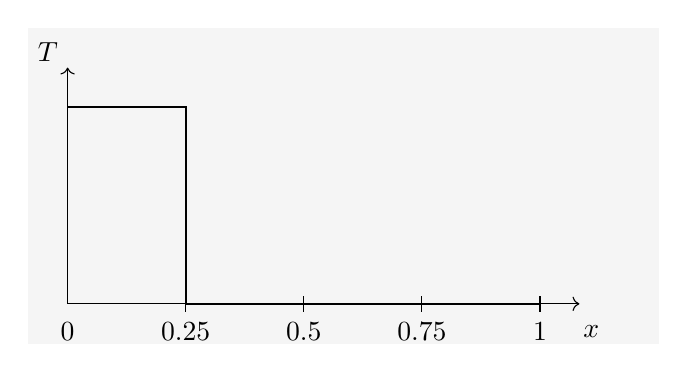
\begin{tikzpicture}
\draw[fill=gray!8,gray!8](0,0) rectangle (8,4);
%\draw[step=0.5cm,gray,very thin] (0,0) grid (8,4); %background grid

\draw[->] (0.5,0.5) -- (7,0.5) ; 
\node[] at (0.5,0.15) {$0$};

\node[] at (2,0.15) {$0.25$};
\node[] at (3.5,0.15) {$0.5$};
\node[] at (5,0.15) {$0.75$};
\node[] at (6.5,0.15) {$1$};
\draw[->] (0.5,0.5) -- (0.5,3.5) ; 
\node[] at (0.25,3.7) {$T$};


\draw[-] (2,0.4) -- (2,0.6) ; 
\draw[-] (3.5,0.4) -- (3.5,0.6) ; 
\draw[-] (5,0.4) -- (5,0.6) ; 
\draw[-] (6.5,0.4) -- (6.5,0.6) ; 


%\draw[-] (2,1) -- (1.75,0.75) ; 
%\draw[-] (2.5,1) -- (2.25,0.75) ; 
%\draw[-] (3,1) -- (2.75,0.75) ; 
%\draw[-] (3.5,1) -- (3.25,0.75) ; 
%\draw[-] (4,1) -- (3.75,0.75) ; 
%\draw[-] (4.5,1) -- (4.25,0.75) ; 

%---------------------------------

%\draw[thick,->] (7,1) -- (7,5) ; 
%\node[] at (6.6,4) {$L_y$};
%\node[] at (6.6,1) {$0$};
%\draw[-] (6.85,1) -- (7.15,1) ; 
%\draw[-] (6.85,4) -- (7.15,4) ; 
%\node[] at (7.6,4) {$p=0$};
%\node[] at (6.6,5) {$y$};

%---------------------------------

\draw[thick] (0.5,3) -- (2,3) -- (2,0.5) -- (6.5,0.5) ; 
\node[] at (7.15,0.15) {$x$};


\end{tikzpicture}



\end{center}

Program the above FTCS method. Run the model for 250 time steps with $\delta t=0.002$. 
Program the Lax-Friedrichs method by modifying the previous code.\\
Bonus: Program the upwind method and/or the Crank-Nicolson method. 

\par\noindent\rule{\textwidth}{0.4pt}
\end{minipage}
\end{center}
%-/-/-/-/-/-/-/-/-/-/-/-/-/-/-/-/-/-/




\newpage
\section{Solving the 1D advection diffusion equation} 
\label{ss:fdm_advdiff1D} \begin{flushright} {\tiny {\color{gray} fdm\_advdiff1D.tex}} \end{flushright}
%~~~~~~~~~~~~~~~~~~~~~~~~~~~~~~~~~~~~~~~~~~~~~~~~~~~~~~~~~~~~~~~~~~~~~~~~~~~~~~~~~~~~~~~~~~~~~~~~~~

The 1d advection-diffusion equation is:
\begin{equation}
\rho C_p \left( \frac{\partial T}{\partial t}  
+ u \frac{\partial T}{\partial x} \right)= k \frac{\partial^2 T}{\partial x^2} + H'
\end{equation}
or simply
\begin{equation}
\frac{\partial T}{\partial t} + u \frac{\partial T}{\partial x}= \kappa \frac{\partial^2 T}{\partial x^2} + H
\end{equation}
where $H=H'/\rho C_p$ is a source term that does not depend on time.
We have seen how to deal with the time derivative (explicit, implicit) 
and with the first order space derivative (forward, backward or central).
Let us consider the FTCS scheme (Forward in Time, Central in Space).
\[
\frac{T_{\color{teal}i}^{n+1}-T^n_{\color{teal}i}}{\delta t} 
+ u_i \frac{T^n_{\color{teal}i+1} - T^n_{{\color{teal}i-1}}}{2h} = \kappa \frac{T_{i+1}^n-2T_i^n+T_{i-1}^n}{h^2} + H_i
\]
Likewise we can consider the BTCS scheme:
\[
\frac{T_{\color{teal}i}^{n+1}-T^n_{\color{teal}i}}{\delta t} 
+ u_i \frac{T^{n+1}_{\color{teal}i+1} - T^{n+1}_{{\color{teal}i-1}}}{2h} 
= \kappa \frac{T_{i+1}^{n+1}-2T_i^{n+1}+T_{i-1}^{n+1}}{h^2} + H_i
\]
which makes the method implicit. 
Or, using a Crank-Nicolson approach:
\[
\frac{T_{\color{teal}i}^{n+1}-T^n_{\color{teal}i}}{\delta t} 
=
\frac12
\left(
- u_i \frac{T^{n+1}n_{\color{teal}i+1} - T^{n+1}_{{\color{teal}i-1}}}{2h} 
+ \kappa \frac{T_{i+1}^{n+1}-2T_i^{n+1}+T_{i-1}^{n+1}}{h^2} 
- u_i \frac{T^n_{\color{teal}i+1} - T^n_{{\color{teal}i-1}}}{2h} + \kappa \frac{T_{i+1}^n-2T_i^n+T_{i-1}^n}{h^2} 
\right)
+ H_i
\]




As we have seen before, the advection term is a source of problems and multiple 
methods have been designed to stabilise the pure advection equation. 
The {\color{olive}Fiadeiro \& Veronis method} \cite{five77,wrig92}, works as follows for the (steady state)
advection-diffusion equation (see also p315 of \textcite{boudreau}):
\[
\kappa \frac{T_{i+1}-2T_i + T_{i-1}}{h^2}
- u \frac{(1-\sigma) T_{i+1}+2\sigma T_i -(1+\sigma)T_{i-1}}{2 h} = 0
\]
which is a blend of backward (upstream) and central differences. The amount of
blending is dictated by the value of the parameter $\sigma$, defined as
\[
\sigma 
= \text{coth} \frac{u h}{2 \kappa} - \frac{2 \kappa}{u h}
= \text{coth} \; \Penb  - \frac{1}{\Penb}
\]
The parameter $\sigma$ has the property that
$\sigma \rightarrow 0$ when $\Penb \rightarrow 0$ and 
$\sigma \rightarrow 1$ when $\Penb \rightarrow \infty$.
The equation above can also be rewritten:
\[
\kappa \frac{T_{i+1}-2T_i + T_{i-1}}{h^2}
- u \frac{1 T_{i+1}-T_{i-1}}{2 h} = 0
+ \frac{u \sigma h}{2} \frac{T_{i+1}-2 T_i +T_{i-1}}{h^2} = 0
\]
which makes the action of this stabilisation term more obvious: it is a diffusion term whose 
diffusion coefficient goes away when $h\rightarrow 0$. 

Thus, if $\sigma = 0$ (diffusion dominated), then pure central differencing is obtained, and if
$\sigma = 1$ (advection dominated), then pure backward differencing results. Interestingly
enough, this blended or weighted scheme is second-order accurate even as it switches
to backward differencing \cite{five77}. 
Note that it is essentially the known streamline upwind method used in FEM or FDM (see
Section~\ref{ss:fdm_adv1D}). 
Also, when $\kappa \rightarrow 0$ (no physical diffusion at all)
then $\sigma$ tends to $\pm 1$, and more precisely: $\sigma = sign(u)$, which allows for a simple 
and elegant implementation. 

Adding a FT time derivative term, the equation above can be rewritten (a source
term has been added):
\[
\frac{T_{\color{teal}i}^{n+1}-T^n_{\color{teal}i}}{\delta t} 
=
\kappa \frac{T_{i+1}^n-2T_i + T_{i-1}^n}{h^2}
- u \frac{(1-\sigma) T_{i+1}^n+2\sigma T_i^n -(1+\sigma)T_{i-1}^n}{2 h} +H 
\]



\paragraph{A simple example} Let us consider the domain $0<x<1$.
Let us prescribe $T(x=0)=0$  and $T(x=1)=0$ and we want to solve 
the steady state advection diffusion equation (with a source term):
\begin{equation}
u \frac{\partial T}{\partial x} = \kappa \frac{\partial^2 T}{\partial x^2} + 1
\label{eq:fdmadvdiff2}
\end{equation}
The solution is then 
\begin{equation}
T(x)=x - \frac{\exp (-(1-x)/\kappa) -\exp (-1/\kappa)  }{1-\exp (-1/\kappa)}
\label{eq:fdmadvdiff1}
\end{equation}

In this case, if $u\rightarrow 0$ then the equation becomes a diffusion equation
and the solution is $T(x)=0$. If $u$ is large, the field is advected to the right
but the right boundary condition $T(x=1)=0$ poses a problem which results in a very steep slope
and potentially numerical issues too for the FTCS method, but not for the FTFV method.

\begin{center}
\includegraphics[width=11cm]{images/fdm/adv_diff/T.pdf}\\
{\captionfont Results obtained with FTCS method. nnx=25, $u=1$, $\delta t=10^{-4}$, 
nstep=25000. FTFV stands for 'forward in time, Fiadeiro \& Veronis'}
\end{center}

A very similar example is implemented in \stone~65 (albeit with FEM).

%-/-/-/-/-/-/-/-/-/-/-/-/-/-/-/-/-/-/-/
\begin{center}
\begin{minipage}[t]{0.77\textwidth}
\par\noindent\rule{\textwidth}{0.4pt}

\begin{center}
\includegraphics[width=0.8cm]{images/garftr} \\
{\color{orange}Exercise FDM-8}
\end{center}

Prove that Eq.~\eqref{eq:fdmadvdiff1} is indeed solution of 
Eq.~\eqref{eq:fdmadvdiff2}. Code the FTCS and FTFV methods and reproduce 
the figure above (i.e. only forward in time/explicit methods).

\par\noindent\rule{\textwidth}{0.4pt}
\end{minipage}
\end{center}
%-/-/-/-/-/-/-/-/-/-/-/-/-/-/-/-/-/-/


\newpage
\section{FDM basics in 2D} \label{ss:fdm_basics2D} 
In a 2D Cartesian domain overlain by a $nnx \times nny$ grid, 
the spacing between nodes in the $x$ and $y$ direction is $h_x$ 
and $h_y$ respectively. 

\begin{center}


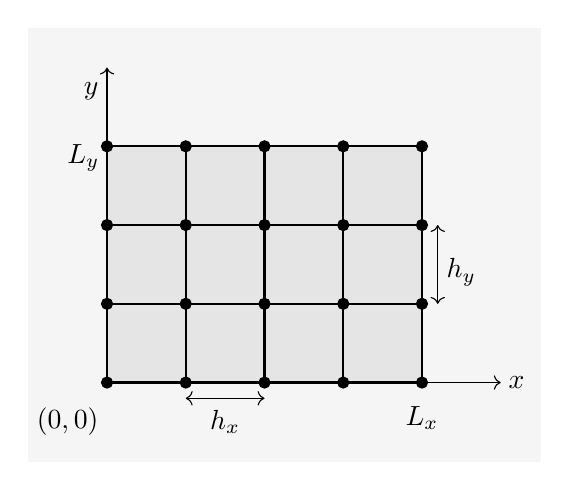
\begin{tikzpicture}
\draw[fill=gray!8,gray!8](0,0) rectangle (6.5,5.5);
%\draw[step=0.5cm,gray,very thin] (0,0) grid (8,5); %background grid


\draw[fill=gray!20,gray!20](1,1) rectangle (5,4);
\draw[thick] (1,1) -- (5,1) -- (5,4) -- (1,4) -- cycle;  

\draw[thick] (1,2) -- (5,2) ; 
\draw[thick] (1,3) -- (5,3) ; 
\draw[thick] (2,1) -- (2,4) ; 
\draw[thick] (3,1) -- (3,4) ; 
\draw[thick] (4,1) -- (4,4) ; 

\draw[black,fill=black] (1,1)  circle (2pt);
\draw[black,fill=black] (2,1)  circle (2pt);
\draw[black,fill=black] (3,1)  circle (2pt);
\draw[black,fill=black] (4,1)  circle (2pt);
\draw[black,fill=black] (5,1)  circle (2pt);
\draw[black,fill=black] (1,2)  circle (2pt);
\draw[black,fill=black] (2,2)  circle (2pt);
\draw[black,fill=black] (3,2)  circle (2pt);
\draw[black,fill=black] (4,2)  circle (2pt);
\draw[black,fill=black] (5,2)  circle (2pt);
\draw[black,fill=black] (1,3)  circle (2pt);
\draw[black,fill=black] (2,3)  circle (2pt);
\draw[black,fill=black] (3,3)  circle (2pt);
\draw[black,fill=black] (4,3)  circle (2pt);
\draw[black,fill=black] (5,3)  circle (2pt);
\draw[black,fill=black] (1,4)  circle (2pt);
\draw[black,fill=black] (2,4)  circle (2pt);
\draw[black,fill=black] (3,4)  circle (2pt);
\draw[black,fill=black] (4,4)  circle (2pt);
\draw[black,fill=black] (5,4)  circle (2pt);

\draw [<->] (5.2,2) -- (5.2,3); \node[] at (5.5,2.4) {$h_y$};
\draw [<->] (2,0.8) -- (3,0.8); \node[] at (2.5,0.5) {$h_x$};

\draw [->] (5,1) -- (6,1); \node[] at (6.2,1) {$x$};
\draw [->] (1,4) -- (1,5); \node[] at (0.8,4.7) {$y$};

\node[] at (0.5,0.5) {$(0,0)$};
\node[] at (5,0.55) {$L_x$};
\node[] at (0.7,3.85) {$L_y$};

%\node[] at (2.2,3.1) {\tiny{\color{brown}i-1,j}};
%\node[] at (3.2,3.1) {\tiny{\color{brown}i,j}};
%\node[] at (4.2,3.1) {\tiny{\color{brown}i+1,j}};

%\node[] at (3.2,4.1) {\tiny{\color{brown}i,j+1}};
%\node[] at (3.2,2.1) {\tiny{\color{brown}i,j-1}};

%\draw[black,fill=black] (3.1,0.2) circle (2pt); \node[] at (3.4,0.2) {$\vec\upnu$};
%\draw (4.1,0.2) circle (4pt); 
%\node[] at (2.5,4.5) {4 vel. nodes, 1 press. nodes};
\end{tikzpicture}

\end{center}

We have seen in Section~\ref{ss:fdm_basics1D} how to discretise second-order derivatives in 1D. 
In 2D, we then logically have for a function $f(x,y)$

\begin{equation}
\frac{\partial^2 f}{\partial x^2}(x_0,y_0) = \frac{f(x_0+h_x,y_0) -2f(x_0,y_0) + f(x_0-h_x,y_0) }{h_x^2} 
+ {\cal O}(h_x^2)
\end{equation}
\begin{equation}
\frac{\partial^2 f}{\partial y^2}(x_0,y_0) = \frac{f(x_0,y_0+h_y) -2f(x_0,y_0) + f(x_0,y_0-h_y) }{h_y^2} 
+ {\cal O}(h_y^2)
\end{equation}
What about mixed derivatives? Since these are combinations of first-order derivatives, 
we can straightforwardly discretise them:
\begin{eqnarray}
&& \frac{\partial^2 f }{\partial x \partial y}(x_0,y_0) \nn\\
&=& \frac{\partial }{\partial x} \left(\frac{\partial f}{\partial y}\right) (x_0,y_0) \nn\\
&=& \frac{\partial }{\partial x} \left(\frac{ f(x_0,y_0+h_y)-f(x_0,y_0-h_y)}{2h_y} \right) \nn\\
&=& \frac{1}{2h_y} \frac{\partial f}{\partial x} (x_0,y_0+h_y)
   -\frac{1}{2h_y} \frac{\partial f}{\partial x} (x_0,y_0-h_y) \nn\\
&=& \frac{1}{2h_y}  \frac{ f(x_0+h_x,y_0+h_y)-f(x_0-h_x,y_0+h_y)}{2h_x} 
-   \frac{1}{2h_y}  \frac{ f(x_0+h_x,y_0-h_y)-f(x_0-h_x,y_0-h_y)}{2h_x}  \nn\\
&=& \frac{f(x_0+h_x,y_0+h_y)-f(x_0-h_x,y_0+h_y)-f(x_0+h_x,y_0-h_y)+f(x_0-h_x,y_0-h_y)}{2 h_x h_y}
+ {\cal O}(h_x^2,h_y^2) \nn
\end{eqnarray}

%...............................
\subsubsection{From 1D to 2D}

INSERT TEXT

\begin{center}
\begin{flushright} {\tiny {\color{gray} (tikz\_needicon.tex)}} \end{flushright}
%~~~~~~~~~~~~~~~~~~~~~~~~~~~~~~~~~~~~~~~~~~~~~~~~~~~~~~~~~~~~~~~~~~~~~~~~~~~~~~~~~~~~~~~~~~~~~~~~~~


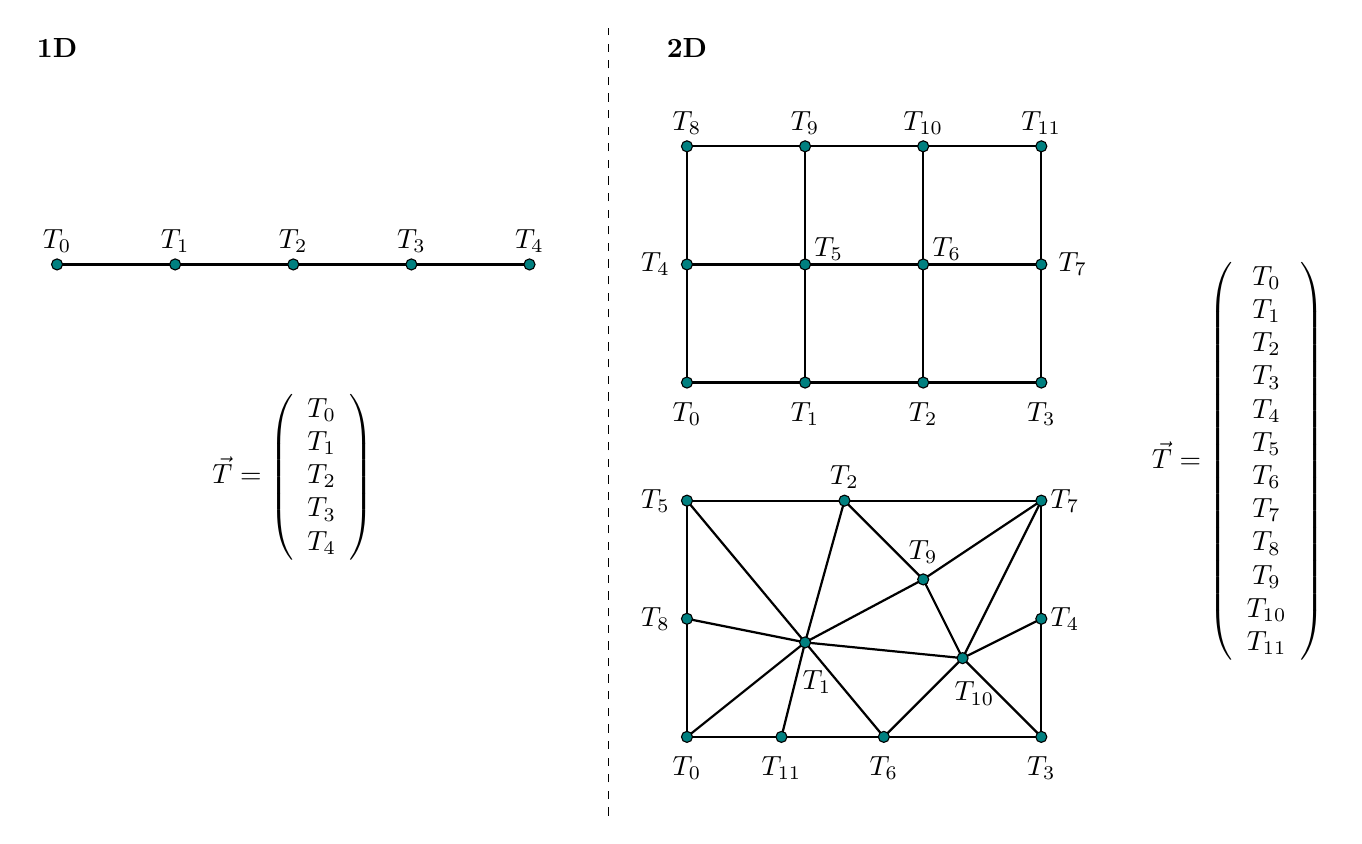
\begin{tikzpicture}
%\draw[step=0.5cm,gray,very thin] (0,0) grid (17,10); 

\node[] at (1,9.75) {\bf 1D};

\draw[thick] (1,7)--(7,7);
\draw[black,fill=teal] (1,7) circle (2pt);
\draw[black,fill=teal] (2.5,7) circle (2pt);
\draw[black,fill=teal] (4,7) circle (2pt);
\draw[black,fill=teal] (5.5,7) circle (2pt);
\draw[black,fill=teal] (7,7) circle (2pt);

\node[] at (1,7.3) {$T_0$};
\node[] at (2.5,7.3) {$T_1$};
\node[] at (4,7.3) {$T_2$};
\node[] at (5.5,7.3) {$T_3$};
\node[] at (7,7.3) {$T_4$};

\node[] at (4,4.3) {
$\vec{T}=\left(
\begin{array}{c}
T_0 \\ T_1 \\ T_2 \\ T_3 \\ T_4
\end{array}
\right)$};

%%%%%%%%%%%%%%%%%%%%%%%%%%%%%%%%%%%%%%%%%55
\draw[dashed] (8,0)--(8,10); 

\node[] at (9,9.75) {\bf 2D};

\draw[thick](9,5.5) rectangle (13.5,8.5);
\draw[thick](9,7)--(13.5,7);
\draw[thick](10.5,5.5)--(10.5,8.5);
\draw[thick](12,5.5)--(12,8.5);

\node[] at (16,4.5) {
$\vec{T}=\left(
\begin{array}{c}
T_0 \\ T_1 \\ T_2 \\ T_3 \\ T_4 \\
T_5 \\ T_6 \\ T_7 \\ T_8 \\ T_9 \\ T_{10} \\ T_{11}
\end{array}
\right)$};

\draw[black,fill=teal] (9,5.5) circle (2pt);
\draw[black,fill=teal] (10.5,5.5) circle (2pt);
\draw[black,fill=teal] (12,5.5) circle (2pt);
\draw[black,fill=teal] (13.5,5.5) circle (2pt);

\draw[black,fill=teal] (9,7) circle (2pt);
\draw[black,fill=teal] (10.5,7) circle (2pt);
\draw[black,fill=teal] (12,7) circle (2pt);
\draw[black,fill=teal] (13.5,7) circle (2pt);

\draw[black,fill=teal] (9,8.5) circle (2pt);
\draw[black,fill=teal] (10.5,8.5) circle (2pt);
\draw[black,fill=teal] (12,8.5) circle (2pt);
\draw[black,fill=teal] (13.5,8.5) circle (2pt);

\node[] at (9,5.1) {$T_0$};
\node[] at (10.5,5.1) {$T_1$};
\node[] at (12,5.1) {$T_2$};
\node[] at (13.5,5.1) {$T_3$};
\node[] at (8.6,7) {$T_4$};

\node[] at (10.8,7.2) {$T_5$};
\node[] at (12.3,7.2) {$T_6$};

\node[] at (13.9,7) {$T_7$};

\node[] at (9,8.8) {$T_8$};
\node[] at (10.5,8.8) {$T_9$};
\node[] at (12,8.8) {$T_{10}$};
\node[] at (13.5,8.8) {$T_{11}$};

%%%%%%%%%%%%%%%%%%%%%%%%%%%%%%%%%%%%%%%5
%triangular mesh

\draw[thick](9,1) rectangle (13.5,4);


\draw[thick](9,1)--(10.5,2.2)--(12,3)--(13.5,4);
\draw[thick](9,4)--(10.5,2.2)--(12.5,2)--(13.5,1);
\draw[thick](11,4)--(12,3)--(12.5,2)--(13.5,2.5);
\draw[thick](13.5,4)--(12.5,2)--(11.5,1)--(10.5,2.2)--(9,2.5);
\draw[thick](10.2,1)--(10.5,2.2)--(11,4);


\draw[black,fill=teal] (9,1) circle (2pt);
\draw[black,fill=teal] (10.2,1) circle (2pt);
\draw[black,fill=teal] (11.5,1) circle (2pt);
\draw[black,fill=teal] (13.5,1) circle (2pt);

\draw[black,fill=teal] (9,2.5) circle (2pt);
\draw[black,fill=teal] (10.5,2.2) circle (2pt);
\draw[black,fill=teal] (12,3) circle (2pt);
\draw[black,fill=teal] (12.5,2) circle (2pt);
\draw[black,fill=teal] (13.5,2.5) circle (2pt);

\draw[black,fill=teal] (9,4) circle (2pt);
\draw[black,fill=teal] (11,4) circle (2pt);
\draw[black,fill=teal] (13.5,4) circle (2pt);

\node[] at (9,0.6) {$T_0$};
\node[] at (10.2,0.6) {$T_{11}$};
\node[] at (11.5,0.6) {$T_6$};
\node[] at (13.5,0.6) {$T_3$};

\node[] at (8.6,2.5) {$T_8$};
\node[] at (8.6,4) {$T_5$};
\node[] at (11,4.3) {$T_2$};
\node[] at (13.8,4) {$T_7$};
\node[] at (13.8,2.5) {$T_4$};

\node[] at (12,3.35) {$T_9$};
\node[] at (12.65,1.55) {$T_{10}$};

\node[] at (10.65,1.7) {$T_1$};

\end{tikzpicture}

\end{center}


Also, here is a rather handy code snippet which should allow you to make nice plots of the coming exercises.

\begin{lstlisting}
       filename = 'solution_{:04d}.pdf'.format(istep) 
       fig = plt.figure ()
       ax = fig.gca(projection='3d')
       ax.plot_surface(x.reshape ((nny,nnx)),y.reshape((nny,nnx)),T.reshape((nny,nnx)),color = 'darkseagreen')
       ax.set_xlabel ( 'X [ m ] ')
       ax.set_ylabel ( 'Y [ m ] ')
       ax.set_zlabel ( ' Temperature  [ C ] ')
       plt.title('Timestep  %.2d' %(istep),loc='right')
       plt.grid ()
       plt.savefig(filename)
       #plt.show ()
       plt.close()
\end{lstlisting}

 
\newpage
\section{Solving the 2D diffusion equation} \label{ss:fdm_diff2D} We now revisit the transient heat equation, this time with sources/sinks for 2D problems.
The heat equation is 
\[
\rho C_p \frac{\partial T}{\partial t} =
\vec\nabla \cdot k \vec\nabla T + Q 
\]
which simply writes as follows when Cartesian coordinates are used:
\[
\rho C_p \frac{\partial T}{\partial t} = 
\frac{\partial }{\partial x} \left(  k  \frac{\partial T}{\partial x} \right)+
\frac{\partial }{\partial y} \left(  k  \frac{\partial T}{\partial y} \right)+
Q
\]
where $Q$ is the radiogenic heat production.

If the heat conductivity is constant, it writes:
\[
\frac{\partial T}{\partial t} =
\kappa \left(  \frac{\partial^2 T}{\partial x^2} +   \frac{\partial^2 T}{\partial y^2} \right)+
\frac{Q}{\rho C_p}
\]

In order to solve this equation over the Cartesian domain of size $L_x \times L_y$
we need to generate a mesh as shown hereunder:
\begin{center}
\includegraphics[width=8cm]{images/fdm/fdgrid}
\end{center}
The spacing between the nodes in the $x$-direction is $h_x$ and $h_y$ is the spacing
between the nodes in the vertical direction. There are now $np=nnx\times nny$ nodes in total.

In one dimension, the subscript indicated the node $i$. In two dimensions we therefore 
need two indices ${\color{brown}i}$ and ${\color{brown}j}$ 
to identify a node, so that the temperature at node ${\color{brown}i},{\color{brown}j}$ 
at time $n$ is denoted $T_{{\color{brown}i,j}}^n$.

%The vector $\vec{T}$ contains all the temperature unknowns, so it is a vector that is $np$-long. 
%But how should this vector be organised ? In other words, 
One question remains: should we number nodes 
row by row ? column by column ? randomly ? 
These three approaches are shown hereunder: 

\vspace{.5cm}

\begin{minipage}[t]{\textwidth}


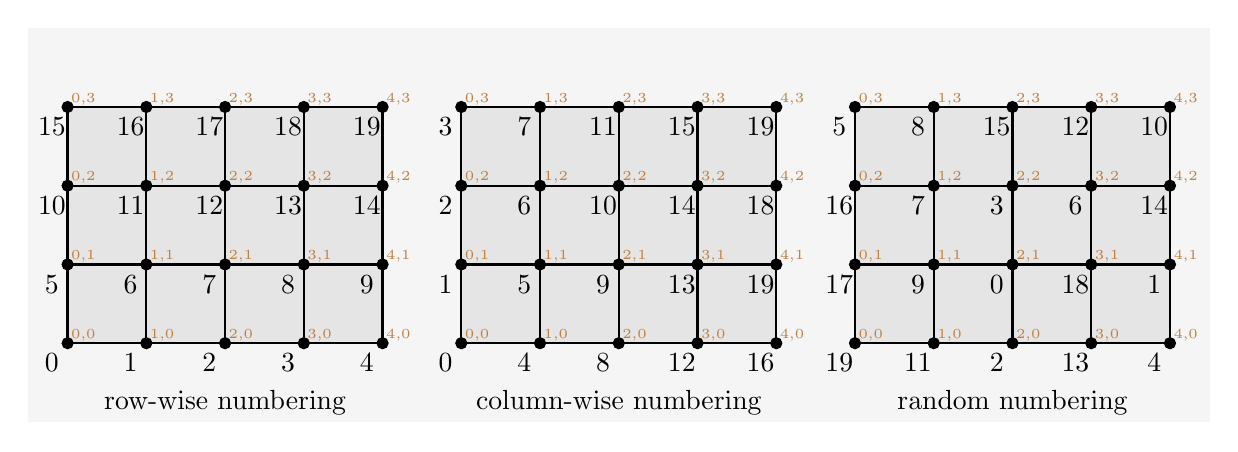
\begin{tikzpicture}
\draw[fill=gray!8,gray!8](0.5,0) rectangle (15.5,5);
%\draw[step=0.5cm,gray,very thin] (0,0) grid (17,5); %background grid

\draw[fill=gray!20,gray!20](1,1) rectangle (5,4);
\draw[fill=gray!20,gray!20](6,1) rectangle (10,4);
\draw[fill=gray!20,gray!20](11,1) rectangle (15,4);

\draw[thick] (1,1) -- (5,1) -- (5,4) -- (1,4) -- cycle;  
\draw[thick] (1,2) -- (5,2) ; 
\draw[thick] (1,3) -- (5,3) ; 
\draw[thick] (2,1) -- (2,4) ; 
\draw[thick] (3,1) -- (3,4) ; 
\draw[thick] (4,1) -- (4,4) ; 
\node[] at (0.8,0.75) {0};
\node[] at (1.8,0.75) {1};
\node[] at (2.8,0.75) {2};
\node[] at (3.8,0.75) {3};
\node[] at (4.8,0.75) {4};
\node[] at (0.8,1.75) {5};
\node[] at (1.8,1.75) {6};
\node[] at (2.8,1.75) {7};
\node[] at (3.8,1.75) {8};
\node[] at (4.8,1.75) {9};
\node[] at (0.8,2.75) {10};
\node[] at (1.8,2.75) {11};
\node[] at (2.8,2.75) {12};
\node[] at (3.8,2.75) {13};
\node[] at (4.8,2.75) {14};
\node[] at (0.8,3.75) {15};
\node[] at (1.8,3.75) {16};
\node[] at (2.8,3.75) {17};
\node[] at (3.8,3.75) {18};
\node[] at (4.8,3.75) {19};
\node[] at (1.2,1.1) {\tiny{\color{brown} 0,0}};
\node[] at (2.2,1.1) {\tiny{\color{brown} 1,0}};
\node[] at (3.2,1.1) {\tiny{\color{brown} 2,0}};
\node[] at (4.2,1.1) {\tiny{\color{brown} 3,0}};
\node[] at (5.2,1.1) {\tiny{\color{brown} 4,0}};
\node[] at (1.2,2.1) {\tiny{\color{brown} 0,1}};
\node[] at (2.2,2.1) {\tiny{\color{brown} 1,1}};
\node[] at (3.2,2.1) {\tiny{\color{brown} 2,1}};
\node[] at (4.2,2.1) {\tiny{\color{brown} 3,1}};
\node[] at (5.2,2.1) {\tiny{\color{brown} 4,1}};
\node[] at (1.2,3.1) {\tiny{\color{brown} 0,2}};
\node[] at (2.2,3.1) {\tiny{\color{brown} 1,2}};
\node[] at (3.2,3.1) {\tiny{\color{brown} 2,2}};
\node[] at (4.2,3.1) {\tiny{\color{brown} 3,2}};
\node[] at (5.2,3.1) {\tiny{\color{brown} 4,2}};
\node[] at (1.2,4.1) {\tiny{\color{brown} 0,3}};
\node[] at (2.2,4.1) {\tiny{\color{brown} 1,3}};
\node[] at (3.2,4.1) {\tiny{\color{brown} 2,3}};
\node[] at (4.2,4.1) {\tiny{\color{brown} 3,3}};
\node[] at (5.2,4.1) {\tiny{\color{brown} 4,3}};
\draw[black,fill=black] (1,1)  circle (2pt);
\draw[black,fill=black] (2,1)  circle (2pt);
\draw[black,fill=black] (3,1)  circle (2pt);
\draw[black,fill=black] (4,1)  circle (2pt);
\draw[black,fill=black] (5,1)  circle (2pt);
\draw[black,fill=black] (1,2)  circle (2pt);
\draw[black,fill=black] (2,2)  circle (2pt);
\draw[black,fill=black] (3,2)  circle (2pt);
\draw[black,fill=black] (4,2)  circle (2pt);
\draw[black,fill=black] (5,2)  circle (2pt);
\draw[black,fill=black] (1,3)  circle (2pt);
\draw[black,fill=black] (2,3)  circle (2pt);
\draw[black,fill=black] (3,3)  circle (2pt);
\draw[black,fill=black] (4,3)  circle (2pt);
\draw[black,fill=black] (5,3)  circle (2pt);
\draw[black,fill=black] (1,4)  circle (2pt);
\draw[black,fill=black] (2,4)  circle (2pt);
\draw[black,fill=black] (3,4)  circle (2pt);
\draw[black,fill=black] (4,4)  circle (2pt);
\draw[black,fill=black] (5,4)  circle (2pt);
%---------------------------------------------------
\draw[thick] (6,1) -- (10,1) -- (10,4) -- (6,4) -- cycle;  
\draw[thick] (6,2) -- (10,2) ; 
\draw[thick] (6,3) -- (10,3) ; 
\draw[thick] (7,1) -- (7,4) ; 
\draw[thick] (8,1) -- (8,4) ; 
\draw[thick] (9,1) -- (9,4) ; 
\node[] at (6.2,1.1)  {\tiny{\color{brown} 0,0}};
\node[] at (7.2,1.1)  {\tiny{\color{brown} 1,0}};
\node[] at (8.2,1.1)  {\tiny{\color{brown} 2,0}};
\node[] at (9.2,1.1)  {\tiny{\color{brown} 3,0}};
\node[] at (10.2,1.1) {\tiny{\color{brown} 4,0}};
\node[] at (6.2,2.1)  {\tiny{\color{brown} 0,1}};
\node[] at (7.2,2.1)  {\tiny{\color{brown} 1,1}};
\node[] at (8.2,2.1)  {\tiny{\color{brown} 2,1}};
\node[] at (9.2,2.1)  {\tiny{\color{brown} 3,1}};
\node[] at (10.2,2.1) {\tiny{\color{brown} 4,1}};
\node[] at (6.2,3.1)  {\tiny{\color{brown} 0,2}};
\node[] at (7.2,3.1)  {\tiny{\color{brown} 1,2}};
\node[] at (8.2,3.1)  {\tiny{\color{brown} 2,2}};
\node[] at (9.2,3.1)  {\tiny{\color{brown} 3,2}};
\node[] at (10.2,3.1) {\tiny{\color{brown} 4,2}};
\node[] at (6.2,4.1)  {\tiny{\color{brown} 0,3}};
\node[] at (7.2,4.1)  {\tiny{\color{brown} 1,3}};
\node[] at (8.2,4.1)  {\tiny{\color{brown} 2,3}};
\node[] at (9.2,4.1)  {\tiny{\color{brown} 3,3}};
\node[] at (10.2,4.1) {\tiny{\color{brown} 4,3}};
\draw[black,fill=black] (6,1)  circle (2pt);
\draw[black,fill=black] (7,1)  circle (2pt);
\draw[black,fill=black] (8,1)  circle (2pt);
\draw[black,fill=black] (9,1)  circle (2pt);
\draw[black,fill=black] (10,1)  circle (2pt);
\draw[black,fill=black] (6,2)  circle (2pt);
\draw[black,fill=black] (7,2)  circle (2pt);
\draw[black,fill=black] (8,2)  circle (2pt);
\draw[black,fill=black] (9,2)  circle (2pt);
\draw[black,fill=black] (10,2)  circle (2pt);
\draw[black,fill=black] (6,3)  circle (2pt);
\draw[black,fill=black] (7,3)  circle (2pt);
\draw[black,fill=black] (8,3)  circle (2pt);
\draw[black,fill=black] (9,3)  circle (2pt);
\draw[black,fill=black] (10,3)  circle (2pt);
\draw[black,fill=black] (6,4)  circle (2pt);
\draw[black,fill=black] (7,4)  circle (2pt);
\draw[black,fill=black] (8,4)  circle (2pt);
\draw[black,fill=black] (9,4)  circle (2pt);
\draw[black,fill=black] (10,4)  circle (2pt);
\node[] at (5.8,0.75) {0};
\node[] at (6.8,0.75) {4};
\node[] at (7.8,0.75) {8};
\node[] at (8.8,0.75) {12};
\node[] at (9.8,0.75) {16};
\node[] at (5.8,1.75) {1};
\node[] at (6.8,1.75) {5};
\node[] at (7.8,1.75) {9};
\node[] at (8.8,1.75) {13};
\node[] at (9.8,1.75) {19};
\node[] at (5.8,2.75) {2};
\node[] at (6.8,2.75) {6};
\node[] at (7.8,2.75) {10};
\node[] at (8.8,2.75) {14};
\node[] at (9.8,2.75) {18};
\node[] at (5.8,3.75) {3};
\node[] at (6.8,3.75) {7};
\node[] at (7.8,3.75) {11};
\node[] at (8.8,3.75) {15};
\node[] at (9.8,3.75) {19};

%---------------------------------------------------
\draw[thick] (11,1) -- (15,1) -- (15,4) -- (11,4) -- cycle;  
\draw[thick] (11,2) -- (15,2) ; 
\draw[thick] (11,3) -- (15,3) ; 
\draw[thick] (12,1) -- (12,4) ; 
\draw[thick] (13,1) -- (13,4) ; 
\draw[thick] (14,1) -- (14,4) ; 
\node[] at (11.2,1.1) {\tiny{\color{brown} 0,0}};
\node[] at (12.2,1.1) {\tiny{\color{brown} 1,0}};
\node[] at (13.2,1.1) {\tiny{\color{brown} 2,0}};
\node[] at (14.2,1.1) {\tiny{\color{brown} 3,0}};
\node[] at (15.2,1.1) {\tiny{\color{brown} 4,0}};
\node[] at (11.2,2.1) {\tiny{\color{brown} 0,1}};
\node[] at (12.2,2.1) {\tiny{\color{brown} 1,1}};
\node[] at (13.2,2.1) {\tiny{\color{brown} 2,1}};
\node[] at (14.2,2.1) {\tiny{\color{brown} 3,1}};
\node[] at (15.2,2.1) {\tiny{\color{brown} 4,1}};
\node[] at (11.2,3.1) {\tiny{\color{brown} 0,2}};
\node[] at (12.2,3.1) {\tiny{\color{brown} 1,2}};
\node[] at (13.2,3.1) {\tiny{\color{brown} 2,2}};
\node[] at (14.2,3.1) {\tiny{\color{brown} 3,2}};
\node[] at (15.2,3.1) {\tiny{\color{brown} 4,2}};
\node[] at (11.2,4.1) {\tiny{\color{brown} 0,3}};
\node[] at (12.2,4.1) {\tiny{\color{brown} 1,3}};
\node[] at (13.2,4.1) {\tiny{\color{brown} 2,3}};
\node[] at (14.2,4.1) {\tiny{\color{brown} 3,3}};
\node[] at (15.2,4.1) {\tiny{\color{brown} 4,3}};
\draw[black,fill=black] (11,1)  circle (2pt);
\draw[black,fill=black] (12,1)  circle (2pt);
\draw[black,fill=black] (13,1)  circle (2pt);
\draw[black,fill=black] (14,1)  circle (2pt);
\draw[black,fill=black] (15,1)  circle (2pt);
\draw[black,fill=black] (11,2)  circle (2pt);
\draw[black,fill=black] (12,2)  circle (2pt);
\draw[black,fill=black] (13,2)  circle (2pt);
\draw[black,fill=black] (14,2)  circle (2pt);
\draw[black,fill=black] (15,2)  circle (2pt);
\draw[black,fill=black] (11,3)  circle (2pt);
\draw[black,fill=black] (12,3)  circle (2pt);
\draw[black,fill=black] (13,3)  circle (2pt);
\draw[black,fill=black] (14,3)  circle (2pt);
\draw[black,fill=black] (15,3)  circle (2pt);
\draw[black,fill=black] (11,4)  circle (2pt);
\draw[black,fill=black] (12,4)  circle (2pt);
\draw[black,fill=black] (13,4)  circle (2pt);
\draw[black,fill=black] (14,4)  circle (2pt);
\draw[black,fill=black] (15,4)  circle (2pt);
\node[] at (10.8,0.75) {19};
\node[] at (11.8,0.75) {11};
\node[] at (12.8,0.75) {2};
\node[] at (13.8,0.75) {13};
\node[] at (14.8,0.75) {4};
\node[] at (10.8,1.75) {17};
\node[] at (11.8,1.75) {9};
\node[] at (12.8,1.75) {0};
\node[] at (13.8,1.75) {18};
\node[] at (14.8,1.75) {1};
\node[] at (10.8,2.75) {16};
\node[] at (11.8,2.75) {7};
\node[] at (12.8,2.75) {3};
\node[] at (13.8,2.75) {6};
\node[] at (14.8,2.75) {14};
\node[] at (10.8,3.75) {5};
\node[] at (11.8,3.75) {8};
\node[] at (12.8,3.75) {15};
\node[] at (13.8,3.75) {12};
\node[] at (14.8,3.75) {10};


\node[] at (3,0.25) {row-wise numbering};
\node[] at (8,0.25) {column-wise numbering};
\node[] at (13,0.25) {random numbering};

\end{tikzpicture}
\\
\begin{center}
{\captionfont Left: row-wise numbering; middle: column-wise ordering; Right: random numbering.
$nnx=5$, $nny=4$ and therefore $np=20$.
}
\end{center}
\end{minipage}

\vspace{.5cm}

This is a critical point because the discretised PDE is formulated as a function of $T_{{\color{brown} i,j}}$ 
with ${\color{brown}i}=0,\dot nnx-1$ and ${\color{brown}j}=0,\dots nny-1$ 
but the vector $\vec{T}$ containing all these values
is indexed by a single index ${\color{teal}k}=0,\dots np-1$. The numbering strategy determines how easy
it is to go from $({\color{brown}i},{\color{brown}j})$ to ${\color{teal}k}$ and vice versa. 
Very concretely again, where does $T_{\color{brown}3,4}$ should be placed in the global 
vector of unknowns $\vec{T}$?

We then need a (preferably simple/straightforward) 'function' 
which associates to every $(i,j)$ a global index $k$. 
For the first grid with row-wise numbering, we have 
$0\leq {\color{brown}i} \leq 4$ , $0 \leq {\color{brown}j} \leq 3$ 
so that $0 \leq {\color{teal}k} \leq 19$
and it follows that 
\[
{\color{teal} k}={\color{brown}j}*nnx+{\color{brown}i}
\]
This is easy to verify: ${\color{brown}i}=3$ and ${\color{brown}j}=2$ 
does correspond to the $13^{th} node$, 
${\color{brown}i}=4$ and ${\color{brown}j}=1$ does correspond to the $9^{th} node$, etc ...

\begin{minipage}[t]{\textwidth}
\begin{center}
\input{tikz_fdm5x4mesh}
\end{center}
\end{minipage}







%.............................
\paragraph{Explicit scheme} The simplest approach is an {\color{olive} FTCS} 
(forward time, centered space) explicit method like in 1D:
\[
\frac{T_{{\color{brown}i,j}}^{n+1}-T_{{\color{brown}i,j}}^n}{\delta t}
= \kappa
\left(
\frac{ T_{{\color{brown}i-1,j}}^{n}-2T_{{\color{brown}i,j}}^{n}+T_{{\color{brown}i+1,j}}^{n}  }{h_x^2} + 
\frac{ T_{{\color{brown}i,j-1}}^{n}-2T_{{\color{brown}i,j}}^{n}+T_{{\color{brown}i,j+1}}^{n}  }{h_y^2}
\right)
+\frac{Q_{{\color{brown}i,j}}^n}{\rho C_p}
\]
where we have assumed that the source term $Q$ can depend of space coordinates and therefore 
appears as $Q_{i,j}$ in the equation.
We define $s_x$ and $s_y$ as follows:
\[
s_x = \frac{\kappa \delta t}{h_x^2}
\quad\quad
s_y = \frac{\kappa \delta t}{h_y^2}
\]
so that
\[
T_{{\color{brown}i,j}}^{n+1} = T_{{\color{brown}i,j}}^n 
+ s_x ( T_{{\color{brown}i-1,j}}^{n}
-2T_{{\color{brown}i,j}}^{n}+T_{i+1,j}^{n} ) 
+s_y ( T_{{\color{brown}i,j-1}}^{n}
-2T_{{\color{brown}i,j}}^{n}
+T_{{\color{brown}i,j+1}}^{n} ) + 
\frac{Q_{{\color{brown}i,j}}^n \delta t}{\rho C_p}
\]
The scheme is stable for  
\[
\delta t \leq \frac{\min(h_x^2,h_y^2)}{2 \kappa}
\]
Boundary conditions can be set the usual way. A constant (Dirichlet) temperature 
at node $(i,j)$ is given by
\[
T_{i,j}=T_{bc} 
\]
where $T_{bc}$ is the prescribed temperature. 

%...........................
\paragraph{Implicit scheme} 
If we now employ a fully implicit, unconditionally stable discretization scheme, the discretised 
PDE becomes:
\[
\frac{T_{i,j}^{n+1}-T_{i,j}^n}{\delta t}
= \kappa
\left(
\frac{ T_{i-1,j}^{n+1}-2T_{i,j}^{n+1}+T_{i+1,j}^{n+1}  }{h_x^2} + 
\frac{ T_{i,j-1}^{n+1}-2T_{i,j}^{n+1}+T_{i,j+1}^{n+1}  }{h_y^2}
\right)
+\frac{Q_{i,j}^n}{\rho C_p}
\]

Rearranging terms with $n+1$ on the left and terms with $n$ on the right hand side gives
\[
-s_x T_{i+1,j}^{n+1}-s_y T_{i,j+1}^{n+1} +(1+2s_x+2s_y)T_{i,j}^{n+1} -s_x T_{i-1,j}^{n+1} -s_y T_{i,j-1}^{n+1} 
=
T_{i,j}^n
+\frac{Q_{i,j}^n \delta t}{\rho C_p}
\]
which here again yields a linear system of equations written ${\bm A}\cdot {\vec T} = {\vec b}$
where ${\bm A}$ is a $(np \times np)$ matrix.



Boundary conditions are $T(x,y)=0$ on all sides, so all nodes 
on the boundary have a prescribed zero temperature\footnote{We assume
here again that these boundary conditions do not change with time.}:
\begin{eqnarray}
T_{\color{brown}0,0} = T_{\color{teal} 0} &=& 0 \nn\\
T_{\color{brown}1,0} = T_{\color{teal} 1} &=& 0 \nn\\
T_{\color{brown}2,0} = T_{\color{teal} 2} &=& 0 \nn\\
T_{\color{brown}3,0} = T_{\color{teal} 3} &=& 0 \nn\\
T_{\color{brown}4,0} = T_{\color{teal} 4} &=& 0 \nn\\
T_{\color{brown}0,1} = T_{\color{teal} 5} &=& 0 \nn\\
T_{\color{brown}4,1} = T_{\color{teal} 9} &=& 0 \nn\\
T_{\color{brown}0,2} = T_{\color{teal} 10} &=& 0 \nn\\
T_{\color{brown}4,2} = T_{\color{teal} 14} &=& 0 \nn\\
T_{\color{brown}0,3} = T_{\color{teal} 15} &=& 0 \nn\\
T_{\color{brown}1,3} = T_{\color{teal} 16} &=& 0 \nn\\
T_{\color{brown}2,3} = T_{\color{teal} 17} &=& 0 \nn\\
T_{\color{brown}3,3} = T_{\color{teal} 18} &=& 0 \nn\\
T_{\color{brown}4,3} = T_{\color{teal} 19} &=& 0 \nn
\end{eqnarray}
In what follows we assume for simplicity and conciseness of notation that 
$h_x=h_y=h$ so that $s_x=s_y=s$ and we will use the notationa $\tilde{Q}=Q \delta t/\rho C_p$
The discretised PDE equation will now be applied to the interior nodes:
\[
-s T_{{\color{brown} i+1,j}}^{n+1}
-s T_{{\color{brown}i,j+1}}^{n+1} 
+(1+4s)T_{{\color{brown}i,j}}^{n+1} 
-s T_{{\color{brown}i-1,j}}^{n+1} 
-s T_{{\color{brown}i,j-1}}^{n+1} 
= T_{{\color{brown}i,j}}^n 
+\tilde{Q}_{{\color{brown}i,j}}^n
\]

\begin{itemize}
\item For node ${\color{teal}k}=6$ (${\color{brown}i}=1,{\color{brown}j}=1$):
\[
-s T_{{\color{brown}2,1}}^{n+1}
-s T_{{\color{brown}1,2}}^{n+1} 
+(1+4s)T_{{\color{brown}1,1}}^{n+1} 
-s T_{{\color{brown}0,1}}^{n+1} 
-s T_{{\color{brown}1,0}}^{n+1} 
= T_{{\color{brown}1,1}}^n +\tilde{Q}_{{\color{brown}1,1}}^n
\]
or, 
\[
-s T_{\color{teal} 7}^{n+1}-s T_{\color{teal} 11}^{n+1} +(1+4s)T_{\color{teal} 6}^{n+1} -s T_{\color{teal} 5}^{n+1} -s T_{\color{teal} 1}^{n+1} 
= T_{\color{teal} 6}^n +\tilde{Q}_{\color{teal} 6}^n
\]

\item For node $k=7$ ($i=2,j=1$):
\item For node $k=8$ ($i=3,j=1$):
\item For node $k=11$ ($i=1,j=2$):
\item For node $k=12$ ($i=2,j=2$):
\item For node $k=13$ ($i=3,j=2$):
\end{itemize}



\begin{landscape}
\[
\left(
\begin{array}{cccccccccccccccccccc}
1 & . & . & . & . & . & . & . & . & . & . & . & . & . & . & . & . & . & . & . \\ %#0
. & 1 & . & . & . & . & . & . & . & . & . & . & . & . & . & . & . & . & . & . \\ %#1
. & . & 1 & . & . & . & . & . & . & . & . & . & . & . & . & . & . & . & . & . \\ %#2
. & . & . & 1 & . & . & . & . & . & . & . & . & . & . & . & . & . & . & . & . \\ %#3
. & . & . & . & 1 & . & . & . & . & . & . & . & . & . & . & . & . & . & . & . \\ %#4
. & . & . & . & . & 1 & . & . & . & . & . & . & . & . & . & . & . & . & . & . \\ %#5
. & -s& . & . & . & -s& {1+4s} & -s& . & . & . & -s & . & . & . & . & . & . & . & . \\ %#6
. & . & -s& . & . & . & -s& {1+4s} & -s& . & . & . & -s & . & . & . & . & . & . & .\\ %#7
. & . & . & -s& . & . & . & -s & {1+4s} & -s & . & . & . & -s & . & . & . & . & . & . \\ %#8
. & . & . & . & . & . & . & . & . & 1 & . & . & . & . & . & . & . & . & . & . \\ %#9
. & . & . & . & . & . & . & . & . & . & 1 & . & . & . & . & . & . & . & . & . \\ %#10
. & . & . & . & . & . &-s & . & . & . & -s& {1+4s} & -s& . & . & .  & -s& . & . & .\\ %#11
. & . & . & . & . & . & . &-s & . & . & . & -s& {1+4s} & -s& . & . & .  & -s& . & .\\ %#12
. & . & . & . & . & . & . & . &-s & . & . & . & -s& {1+4s} & -s& . & . & .  & -s & .\\ %#13
. & . & . & . & . & . & . & . & . & . & . & . & . & . & 1 & . & . & . & . & . \\ %#14
. & . & . & . & . & . & . & . & . & . & . & . & . & . & . & 1 & . & . & . & . \\ %#15
. & . & . & . & . & . & . & . & . & . & . & . & . & . & . & . & 1 & . & . & . \\ %#16
. & . & . & . & . & . & . & . & . & . & . & . & . & . & . & . & . & 1 & . & . \\ %#17
. & . & . & . & . & . & . & . & . & . & . & . & . & . & . & . & . & . & 1 & . \\ %#18
. & . & . & . & . & . & . & . & . & . & . & . & . & . & . & . & . & . & . & 1    %#19
\end{array}
\right)
\cdot
\underbrace{
\left(
\begin{array}{c}
T_{\color{teal}0} \\ 
T_{\color{teal}1} \\ 
T_{\color{teal}2} \\ 
T_{\color{teal}3} \\ 
T_{\color{teal}4} \\ 
T_{\color{teal}5} \\ 
T_{\color{teal}6} \\ 
T_{\color{teal}7} \\ 
T_{\color{teal}8} \\ 
T_{\color{teal}9} \\ 
T_{\color{teal}10} \\ 
T_{\color{teal}11} \\ 
T_{\color{teal}12} \\ 
T_{\color{teal}13} \\ 
T_{\color{teal}14} \\ 
T_{\color{teal}15} \\ 
T_{\color{teal}16} \\ 
T_{\color{teal}17} \\ 
T_{\color{teal}18} \\ 
T_{\color{teal}19} 
\end{array}
\right)
}_{\vec T}
=
\underbrace{
\left(
\begin{array}{c}
0\\ 
0\\ 
0\\ 
0\\ 
0\\ 
0\\ 
T_{{\color{teal}6}}^n + \tilde{Q}_{\color{teal}6} \\ 
T_{{\color{teal}7}}^n + \tilde{Q}_{\color{teal}7} \\ 
T_{{\color{teal}8}}^n + \tilde{Q}_{\color{teal}8} \\ 
0\\ 
0\\ 
T_{{\color{teal}11}}^n + \tilde{Q}_{\color{teal}11} \\ 
T_{{\color{teal}12}}^n + \tilde{Q}_{\color{teal}12} \\ 
T_{{\color{teal}13}}^n + \tilde{Q}_{\color{teal}13} \\ 
0\\ 
0\\ 
0\\ 
0\\ 
0\\ 
0 
\end{array}
\right)
}_{\vec b}
\]
\end{landscape}


Note that we now have five diagonals filled with non-zero entries as opposed to three
diagonals in the 1D case.






\section{Solving the 2D advection-diffusion equation} \label{ss:fdm_advdiff2D} 
So far, we have mainly focused on the diffusion equation in a non-moving domain 
(relevant for the case of a dike intrusion cooling off 
or for a lithosphere which remains undeformed). 

We now want to consider problems where material moves during the time period under 
consideration and takes temperature anomalies with it (e.g. a plume rising 
through a convecting mantle). 
If the numerical grid remains fixed in the background, the hot temperatures should 
be moved to different grid points at each time step. 

We start again from the heat transport equation of Section~\ref{ss:hte}:
\begin{equation}
\rho C_p \left( \frac{\partial T}{\partial t} + \vec\upnu \cdot \vec\nabla T  \right)=
\vec\nabla \cdot k \vec\nabla T + Q 
\end{equation}
In one-dimensional Cartesian coordinates:
\begin{equation}
\rho C_p \left( \frac{\partial T}{\partial t}  
+ u \frac{\partial T}{\partial x} \right)= 
\frac{\partial }{\partial x} \left(  k  \frac{\partial T}{\partial x} \right)+ Q
\end{equation}
and in 2D
\begin{equation}
\rho C_p \left( \frac{\partial T}{\partial t}   
+ u \frac{\partial T}{\partial x}  
+ v \frac{\partial T}{\partial y} \right) 
=
\frac{\partial }{\partial x} \left(  k  \frac{\partial T}{\partial x} \right)
+
\frac{\partial }{\partial y} \left(  k  \frac{\partial T}{\partial y} \right)
+Q
\end{equation}
and in the case where $k$ is constant in space:
\begin{equation}
\frac{\partial T}{\partial t}   
+ u \frac{\partial T}{\partial x}  
+ v \frac{\partial T}{\partial y} 
=
\kappa \left( 
\frac{\partial^2 T}{\partial x^2} 
+ \frac{\partial^2 T}{\partial y^2} \right) +Q
\end{equation}
Since we have already seen how to deal with 'pure' diffusion equations in the 
previous section, let us now turn to 'pure' advection equations:

\begin{equation}
\frac{\partial T}{\partial t}  + u \frac{\partial T}{\partial x} = 0
\end{equation}
or
\begin{equation}
\frac{\partial T}{\partial t}  + u \frac{\partial T}{\partial x} + v \frac{\partial T}{\partial y}= 0
\end{equation}
where we assume $\vec\upnu=(u,v)$ known. 

Even though the equations appear simple, it is quite tricky to solve them accurately, 
more so than for the diffusion problem. 
This is particularly the case if there are large gradients in the quantity that is to be advected. 







\newpage
\section{FEM vs FDM?}\label{ss:femvsfdm}   
Let us start with the 1D steady advection-diffusion equation:
\begin{equation}
\rho C_p u \frac{dT}{dx} - k \frac{d^2T}{dx^2} = f \qquad \text{in} \quad [0,L_x]
\label{eq:fdm1Dad}
\end{equation}
with the boundary conditions $T(x=0)=0$ and $T(x=L_x)=0$.

We have seen before (see Section~\ref{XXX}) 
that the elemental matrix ${\bm K}_a$ for the advection and 
the elemental matrix  ${\bm K}_d$ for the diffusion terms are
\[
{\bm K}_a^e = \frac{\rho C_p u}{2} 
\left(
\begin{array}{cc}
-1 & 1 \\
-1 & 1 
\end{array}
\right)
\qquad
{\bm K}_d^e=\frac{k}{h_x}
\left(
\begin{array}{cc}
1 & -1 \\ 
-1 & 1
\end{array}
\right)
\]
where $h_x$ is the distance between nodes in the $x$-direction 
and $e$ denotes the element number. 

Assuming that we have 5 elements (i.e. 6 nodes), the assembled $6\times 6$ 
advection and diffusion matrices 
(before boundary conditions are applied) are:
\[
{\bm K}_a
= \frac{\rho C_p u}{2}
\left(
\begin{array}{cccccc}
-1 & 1 & 0 & 0 & 0  &0\\
-1 & 0 & 1 & 0 & 0  &0\\
 0 &-1 & 0 & 1 & 0  &0\\
 0 & 0 &-1 & 0 & 1  &0\\
 0 & 0 & 0 &-1 & 0  &1\\
 0 & 0 & 0 & 0 &-1  &1\\
\end{array}
\right)
\qquad
{\bm K}_d
= \frac{k}{h_x}
\left(
\begin{array}{cccccc}
 1 &-1 & 0 & 0 & 0 &  0\\
-1 & 2 &-1 & 0 & 0 &  0\\
 0 &-1 & 2 &-1 & 0 &  0\\
 0 & 0 &-1 & 2 &-1 &  0\\
 0 & 0 & 0 &-1 & 2 & -1\\
 0 & 0 & 0 & 0 &-1 &  1\\
\end{array}
\right)
\]
The rhs is zero, so that we would have to solve $({\bm K}_a+{\bm K}_d)\cdot \vec{T}=0$ 
, or:
\[
\left[ 
\frac{\rho C_p u}{2}
\left(
\begin{array}{cccccc}
-1 & 1 & 0 & 0 & 0  &0\\
-1 & 0 & 1 & 0 & 0  &0\\
 0 &-1 & 0 & 1 & 0  &0\\
 0 & 0 &-1 & 0 & 1  &0\\
 0 & 0 & 0 &-1 & 0  &1\\
 0 & 0 & 0 & 0 &-1  &1\\
\end{array}
\right)
+
\frac{k}{h_x}
\left(
\begin{array}{cccccc}
 1 &-1 & 0 & 0 & 0 &  0\\
-1 & 2 &-1 & 0 & 0 &  0\\
 0 &-1 & 2 &-1 & 0 &  0\\
 0 & 0 &-1 & 2 &-1 &  0\\
 0 & 0 & 0 &-1 & 2 & -1\\
 0 & 0 & 0 & 0 &-1 &  1\\
\end{array}
\right)
\right]
\cdot
\left(
\begin{array}{c}
T_1 \\ T_2 \\ T_3 \\ T_4 \\ T_5 \\ T_6
\end{array}
\right)
= \vec{0}
\]
Note that boundary conditions are not applied yet. 
Therefore the algebraic equation for an interior node $i$ is 
\[
\rho C_p u
\frac{T_{i+1}-T_{i-1}}{2}
+
\frac{k}{h_x}
(-T_{i-1}+2T_i-T_{i+1}) = 0
\]
or, 
\begin{equation}
\boxed{
\rho C_p u
\frac{T_{i+1}-T_{i-1}}{2h_x}
-
\frac{k}{h_x^2}
(T_{i-1}-2T_i+T_{i+1}) = 0
} \label{eq:fdm1Ddiscr}
\end{equation}

However, we have seen in Section~\ref{fdm_basics1D} that the 
second order accurate central differencing based approximate first and second
derivatives written for an interior node $i$ 
of a finite difference mesh with a constant node spacing of $h$ is 
\[
\left. \frac{dT}{dx}\right|_i
\simeq \frac{T_{i+1}-T_{i-1}}{2 h_x}
\qquad
\frac{d^2T}{dx^2} 
\simeq \frac{T_{i+1}-2T_i+T_{i-1}}{h_x^2}
\]
Using these approximations, the discretised formualtion of Eq.~(\ref{eq:fdm1Dad}) is
exactly the same as Eq.~(\ref{eq:fdm1Ddiscr}).
This simple example proves that the FEM and the FDM share similarities!


It is also useful to introduce the elemental Peclet number
\[
Pe = \frac{uh}{2 \kappa} = \frac{u h \rho C_p}{2 k}
\]
\index{general}{Peclet Number}
and Eq.~(\ref{eq:fdm1Dad}) becomes:
\[
\frac{u}{2h_x}
\left[
\left(1-\frac{1}{Pe}\right) T_{i+1} + \frac{2}{Pe} T_i - \left(1+\frac{1}{Pe}\right)T_{i-1} 
\right] = f
\]
CHECK!!!














\newpage
\section{GEO4-1427: vorticity-streamfunction project} \begin{flushright} {\tiny {\color{gray} geo1427project.tex}} \end{flushright}
%~~~~~~~~~~~~~~~~~~~~~~~~~~~~~~~~~~~~~~~~~~~~~~~~~~~~~~~~~~~~~~~~~~~~~~~~~~~~


We consider a 2D Cartesian domain. We wish to solve the incompressible 
isothermal Stokes equations in this domain using the 
vorticity-streamfunction approach (see Section~\ref{ss:vorticitystreamfunction}). 
We assume that the fluids in the domain all have the same viscosity 
$\eta_0$ and that the gravity is vertical 
and pointing downwards, i.e.  $\vec{g}=(g_x,g_y)=(0,-g_0)$.
The density in the domain is given by a  function $\rho(x,y)$ specified
here after. In what follows the boundary conditions are assumed to be free slip. 

\begin{itemize}
\item
Experiment 1: the domain is a square of size 600~\si{\km}.  
It contains two fluids, the `mantle'  and the `slab'. 
The mantle has a density of 3200~\si{\kg\per\cubic\meter} 
and fills the domain except for a circle (the slab) of radius 100~\si{\km} 
centered at $x=L_x/2$ and $y=\frac23 L_y$  of density 
3300~\si{\kg\per\cubic\meter}. $g_0=10~\si{\meter\per\square\second}$ 
and $\eta_0=10^{21}~\si{\pascal\second}$.

\begin{center}
\includegraphics[width=5cm]{images/fdm/project/rho1}
\end{center}

\item
Experiment 2: 
gravity field ($g_x=0$, $g_y=10~\si{\meter\per\square\second}$) 
for a density structure with two vertical layers 
(3200~\si{\kg\per\cubic\meter} and 3300~\si{\kg\per\cubic\meter} 
for the left and right layers, respectively). The model size is  
$1500~\si{\km} \times 1000~\si{\km}$.
Use a constant viscosity $\eta = 10^{21}~\si{\pascal\second}$ 
for the entire model.
\end{itemize}

\begin{center}
\includegraphics[width=5cm]{images/fdm/project/rho2}
\end{center}

%--------------------------------
\subsection*{Background theory}

We start from 
\begin{equation}
\vec\nabla^4 \psi = \frac{1}{\eta_0} \left( -\frac{\partial (\rho g_x)}{\partial y}
+\frac{\partial (\rho g_y)}{\partial x} \right)
\label{eq:md40XX}
\end{equation}
where
\[
\vec\nabla^4 = 
\left( 
\frac{\partial^2 }{\partial x^2} + \frac{\partial^2 }{\partial y^2} 
\right) 
\left( 
\frac{\partial^2 }{\partial x^2} + \frac{\partial^2 }{\partial y^2} 
\right) 
\]
Eq.~\eqref{eq:md40XX} can be rewritten as two Poisson equations, by 
defining the vorticity as $\omega = \vec\nabla^2 \psi$:

We obtain 
the Poisson equation for the vorticity $\omega$:
\begin{equation}
\vec\nabla^2 \omega = -\frac{1}{\eta_0} \left( -\frac{\partial (\rho g_x)}{\partial y}
+\frac{\partial (\rho g_y)}{\partial x} \right)
\end{equation}
In what follows we assume that the domain is a Cartesian box aligned 
with the $x,y$ axis. The gravity is constant and vertical so that $g_x=0$ and 
then we must solve 
\begin{eqnarray}
\vec\nabla^2 \omega &=& -\frac{g_0}{\eta_0}  \frac{\partial \rho}{\partial x} \label{eq:poiss1} \\
\vec\nabla^2 \psi &=& \omega  \label{eq:poiss2} 
\end{eqnarray}


\begin{enumerate}
\item The domain under consideration is a rectangle of size $L_x \times L_y$. Create a mesh of $nnx \times nny$ nodes. 
Store the $x$ and $y$ coordinates in 2 arrays {\tt xcoords} and {\tt ycoords}
\item Prescribe the density $\rho$ on the nodes of the mesh, store the values in the {\tt rho} array. 
Visualise this field and produce a figure called {\sl rho.png}.
\item Compute $\partial \rho/ \partial x$ on the nodes. Visualise this field and produce a figure called {\sl drhodx.png}. 
Use a centered approach if a node is inside the domain and a backward or forward approach if it is on a boundary.
\item Solve Eq.~\eqref{eq:poiss1} using the FD method. Solve the linear system with a scipy solver. Boundary conditions for $\omega$ are $\omega=0$ on all four sides of the domain.
Visualise this field and produce a figure called {\sl omega.png}
\item Solve Eq.~\eqref{eq:poiss2} in a similar way, also setting $\psi=0$ on all four sides.
Visualise this field and produce a figure called {\sl psi.png}
\item Compute the velocity components $u$ and $v$ at each node using 
\[
u=\frac{\partial \psi}{\partial y} 
\qquad \text{and} \qquad
v=-\frac{\partial \psi}{\partial x} 
\]
As in question 2, use the appropriate stencil whether a node is on a boundary or not.
Test your implementation of the gradients by computing $u,v$ at each node having set $\psi=1$ on all nodes
(test 1) and set $\psi=xy$ on all nodes (test 2). In both cases, what values of $u,v$ do we expect? 
Do you recover these values? (if not there is a problem here and you should not proceed any further 

When this is correct, visualise the velocity components (in cm/year!) for the sinking sphere: produce then 
two files, {\sl u.png} and {\sl v.png}, and also a third file {\sl vel.png} 
with the density overlain by velocity vectors. 

\item Compute the strain rate tensor components
\[
\dot\varepsilon_{xx} =\frac{\partial u}{\partial x} 
\qquad
\dot\varepsilon_{yy} =\frac{\partial v}{\partial y} 
\qquad
\dot\varepsilon_{xy} = \frac12 \left(\frac{\partial u}{\partial y} + \frac{\partial v}{\partial x} \right)
\]
Visualise these fields and produce then three files {\sl exx.png}, {\sl eyy.png} and {\sl exy.png}.

\item Compute the effective strain rate
\[
\varepsilon_e = \sqrt{ \frac{1}{2}(\dot\varepsilon_{xx}^2 + \dot\varepsilon_{yy}^2 ) + \dot\varepsilon_{xy}^2  }
\]
and produce a figure {\sl ee.png}

\item Bonus: try the 9 point Laplace stencil, see Section~\ref{ss:ninepointstencil}.

\end{enumerate}



\newpage
\section{Solving the 2D Stokes equations} \label{ss:fdm_stokes2D} \begin{flushright} {\tiny {\color{gray} \tt fdm\_stokes2D.tex}} \end{flushright}
%~~~~~~~~~~~~~~~~~~~~~~~~~~~~~~~~~~~~~~~~~~~~~~~~~~~~~~~~~~~~~~~~~~~~~~~~~~~~~~~~~~~~~~~~~~~~~~~~~~

%---------------------------------------------------------
\subsection{A quick recap of the incompressible 2D Stokes equations}

In the case of an incompressible and isoviscous flow, we can start  from the momentum equation
\begin{equation}
-\vec\nabla p + \vec\nabla \cdot {\bm \tau} + \rho \vec{g} = \vec{0}
\end{equation}
with\footnote{Since the flow is incompressible we will not distinguish
between the strain rate tensor and the deviatoric strain rate tensor 
since they are identical.} 
\begin{equation}
{\bm \tau} = 2 \eta \dot{\bm \varepsilon}(\vec\upnu)
\end{equation}
In 2D the strain rate tensor components are given by
\[
\dot{\varepsilon}_{xx}=\frac{\partial u}{\partial x}
\quad\quad\quad
=\dot{\varepsilon}_{yx}
=\frac{1}{2} \left( \frac{\partial u}{\partial y} + \frac{\partial v}{\partial x} \right)
\quad\quad\quad
\dot{\varepsilon}_{yy}=\frac{\partial v}{\partial y}
\]
In the end we obtain the following set of coupled PDEs for the three 
unknwons $u,v,p$:
\begin{eqnarray}
-\frac{\partial p}{\partial x}  
+ 2 \frac{\partial }{\partial x} \left(\eta \frac{\partial u}{\partial x}  \right) 
+\frac{\partial}{\partial y}\left(\eta (\frac{\partial u}{\partial y}+\frac{\partial v}{\partial x}) \right)
+  \rho g_x &=&0 \\
-\frac{\partial p}{\partial y}  
+ 2 \frac{\partial }{\partial y} \left(\eta \frac{\partial v}{\partial y}  \right) 
+\frac{\partial}{\partial x}\left(\eta (\frac{\partial u}{\partial y}+\frac{\partial v}{\partial x}) \right)
+  \rho g_y  &=& 0 \\
\frac{\partial u}{\partial x} + \frac{\partial v}{\partial y}  = 0 
\end{eqnarray}

Note that in their syllabus \textcite{beka} add the term $p/\lambda$ to the rhs
of the incompressibility equation: 
\begin{displayquote}
{\color{darkgray}
This is a ``trick'' called
the penalty method, which ensures that the system of equations does not become ill-
posed. For this to work, $\lambda$ should be sufficiently large 
($\sim 10^4$ or so), so that the condition
of incompressibility is approximately satisfied.}
\end{displayquote} 


Then, {\it if the viscosity is constant} the $x$-component of 
the momentum conservation equation
\[
-\frac{\partial p}{\partial x}  
+ 2\eta \frac{\partial \dot{\varepsilon}_{xx}}{\partial x} 
+ 2\eta \frac{\partial \dot{\varepsilon}_{xy}}{\partial y}  + \rho g_x =0
\]
becomes
\[
-\frac{\partial p}{\partial x}  
+ 2\eta \frac{\partial^2 u}{\partial x^2} 
+ \eta \left( \frac{\partial^2 u}{\partial y^2 } 
+ \frac{\partial^2 v}{\partial x \partial y} \right)  \rho g_x =0
\]
Using ${\vec \nabla} \cdot {\vec v} = 0$ to obtain 
$\frac{\partial u}{\partial x} =  - \frac{\partial v}{\partial y}  $ we arrive at 
\[
-\frac{\partial p}{\partial x}  
+ \eta \left( \frac{\partial^2 u}{\partial x^2} 
+ \frac{\partial^2 u}{\partial y^2 }  \right)
+ \rho g_x =0
\]
The same approach can be carried out for the $y$-component of the momentum conservation
equation and in the end
these are the three coupled equations we need to solve
\begin{eqnarray}
-\frac{\partial p}{\partial x}  
+ \eta \left( \frac{\partial^2 u}{\partial x^2} 
+ \frac{\partial^2 u}{\partial y^2 }  \right) + \rho g_x &=&0 \\
-\frac{\partial p}{\partial y}  
+ \eta \left( \frac{\partial^2 v}{\partial x^2} 
+ \frac{\partial^2 v}{\partial y^2 }  \right) + \rho g_y  &=& 0 \\
\frac{\partial u}{\partial x} + \frac{\partial v}{\partial y}  = 0 
\end{eqnarray}
Of course these PDEs must be supplemented by appropriate boundary conditions.

At this stage we must acknowledge (as in the FEM case) that it would be pointless
to blindly discretise the equations above. Much work has been done on the topics
for decades and only certain approaches have proven succesful. 
The book of Taras Gerya (1st and second edition \cite{gery10,gery19book}) 
remains the reference in geodynamics and what follows is greatly influenced by this book. 


%--------------------------------------------
\subsection{A quick note about the MAC sheme}

The MAC scheme originates in \textcite{hawe65} (1965) and is nicely
summed up in \textcite{kans08} (2008) and \textcite{mctf08} (2008).
Before going any further we need to highlight a few points from the original paper.
First, 
\begin{displayquote}
{\color{darkgray}
One point should be emphasized. The marker particles introduced into 
this incompressible flow calculation are only for the purpose 
of indicating fluid configuration. They show which cells contain fluid
and especially which cells lie along the free surface. [...]
They do not participate in the calculation as do the Particle-in-Cell-method
particles in the Los alamos computer program for compressible flows.
}
\end{displayquote}
Second, looking at ther equations
\begin{center}
\fbox{\includegraphics[width=7cm]{images/fdm/hawe65_a}}
\end{center}
we read that $\varphi$ is the ratio of the pressure to the (constant) density
and that $\nu=\eta/\rho$ is the kinematic viscosity coefficient. 
This constant-density approximation is quite limiting in the context 
of geodynamics where buoyancy-driven flow is important so 
we will not pursue this direction further. Likewise the constant-viscosity
approximation is also not desirable.

Before moving on, it is quite interesting that 
when looking at their Fig.~2, we find that the spatial 
layout of the unknowns is of the staggered type:
\begin{center}
\fbox{\includegraphics[width=7cm]{images/fdm/hawe65_b}}
\end{center}



%------------------------------------
\subsection{The fully staggered grid}

Let us consider a 2D Cartesian domain of size $L_x \times L_y$.
It can be shown that the following layout of nodes is necessary 
if the FDM is to be successful\footnote{In other words
any attempt where $u$, $v$, $p$ would be on the corner nodes is doomed.}:
Note that in what follows we consider a mesh where all nodes are equidistant.
This is not a requirement of the method but it allows for more compact notations
\footnote{We will revisit this topic in Section~\ref{ss:fdm_stokes_hvar}.}. 

We find a similar staggered grid figure in Gerya's book:

\input{tikz/tikz_staggered2D}

There are:
\begin{itemize}
\item ${ncell}={ ncellx}\cdot { ncelly}={ ncell}$ cells ($5\cdot 4$ above)
\item ${N_p}={ ncell}$ pressure values ($20$ above)
\item ${N_u}={ (ncellx+1)}\cdot { ncelly}$ $u$ unknowns ($6\cdot 4$ above) 
\item ${N_p}={ ncell}\cdot { (ncelly+1)}$ $v$ unknowns ($5\cdot 5$ above) 
\item each cell is of size $h_x \cdot h_y$ 
with $h_x=L_x/{ ncellx}$ and $h_y=L_y/{ ncelly}$.
\end{itemize}
In total there are (not taking boundary conditions into account)
$N$ unknowns with:
\[
N=N_u+N_v+N_p
= { (ncellx+1)}\cdot{ ncelly}
+ { ncell}\cdot{ (ncelly+1)}
+ { ncellx}]\cdot{ ncelly} 
\]
Note: the number of $u$ unknowns is not necessarily equal to the number of $v$
unknowns! This is nearly always the case with FEM. 

This means that once we have discretised the Stokes equations we will need
as many (i.e. $N$) equations in order to obtain a linear system with a solution.


\begin{center}
\includegraphics[width=6cm]{images/fdm/gerya_A}\\
{\captionfont Taken from Gerya (2019).}
\end{center}

What follows is mostly borrowed from Taras Gerya's book (second edition). 
However I do not like the notations of the book (or rather they do not match
with the ones of this project) so I have changed them (in particular I use 
the `{\tt n-e-w-s}' system, i.e. north-east-west-south, 
and I prefer $\tau$ to  $\sigma'$ for the deviatoric stress tensor.
Also I feel that it makes more sense to start with a regular mesh 
where all cells have the same size $h_x \times h_y$ (as opposed to the book).
Finally, in the book the $y$-axis points downwards while 'my' $y$-axis 
points upwards.

In what follows we assume that we know the value of the density $\rho$
and viscosity $\eta$ on the (black) nodes of the mesh. We here only focus on the 
Stokes equations (mass and momentum conservation equations) and leave the energy
equation aside.

The justification for the particular approach taken below to 
discretise the equations stems from the concept of conservative 
finite differences explained in Section 7.3 of Gerya's book. 


%\newpage
%...............................................
\subsection{Momentum equation: $x$-component}

Let us zoom-in on a node which carries a $u$ unknown. 
We label it ${\color{violet}u_\otimes}$. Its right ('east')  
neighbour is then ${\color{violet}u_{\tt e}}$,
its left ('west') neighbour is ${\color{violet}u_{\tt w}}$, 
its top ('north') neighbour is ${\color{violet}u_{\tt n}}$ and 
its bottom ('south') neighbour is ${\color{violet}u_{\tt s}}$.
Its nearest pressure nodes are ${\color{teal}p_{\tt e}}$ and 
${\color{teal}p_{\tt w}}$, and the $v$ nodes
that surround it are ${\color{orange}v_{\tt sw}}$, 
${\color{orange}v_{\tt se}}$, ${\color{orange}v_{\tt ne}}$ and 
${\color{orange}v_{\tt nw}}$ as shown here:


\begin{multicols}{2}
\begin{flushright} {\tiny {\color{gray} (tikz\_staggered2D\_u.tex)}} \end{flushright}
%~~~~~~~~~~~~~~~~~~~~~~~~~~~~~~~~~~~~~~~~~~~~~~~~~~~~~~~~~~~~~~~~~~~~~~~~~~~~~~~~~~~~~~~~~~~~~~~~~~

\begin{center}
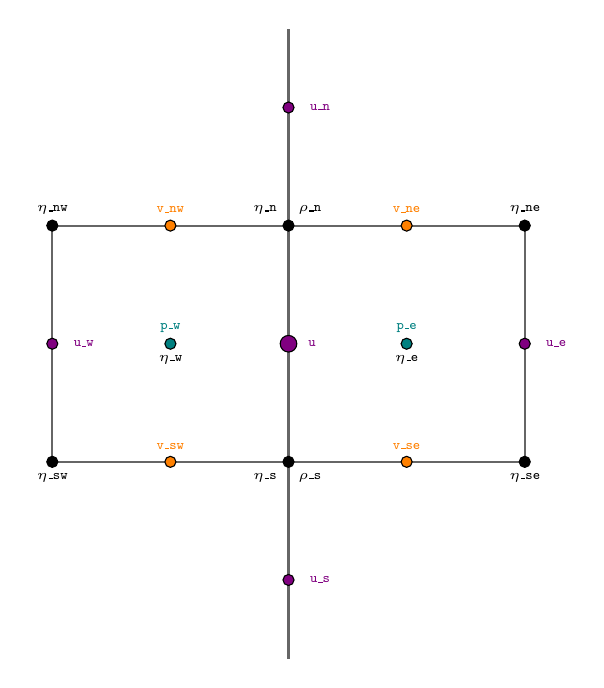
\begin{tikzpicture}
%\draw[fill=gray!23,gray!23](0,0) rectangle (8,9);
%\draw[step=0.5cm,gray,very thin] (0,0) grid (8,9); %background grid

\draw[thick,black!60] (1,3) -- (7,3) -- (7,6) -- (1,6) -- cycle ; 
\draw[thick,black!60] (4,0.5) -- (4,8.5)  ;   

%---------------------------------------------------
\node[] at (2.5,6.2) {\tiny \color{orange} \tt v\_nw};
\node[] at (2.5,3.2) {\tiny \color{orange} \tt v\_sw};
\node[] at (5.5,6.2) {\tiny \color{orange} \tt v\_ne};
\node[] at (5.5,3.2) {\tiny \color{orange} \tt v\_se};
\draw[black,fill=orange] (2.5,6)   circle (2pt);
\draw[black,fill=orange] (2.5,3)   circle (2pt);
\draw[black,fill=orange] (5.5,6)   circle (2pt);
\draw[black,fill=orange] (5.5,3)   circle (2pt);

%--------------------------------------------------
\draw[black,fill=violet] (4,1.5)   circle (2pt);
\draw[black,fill=violet] (4,4.5)   circle (3pt);
\draw[black,fill=violet] (4,7.5)   circle (2pt);
\draw[black,fill=violet] (1,4.5)   circle (2pt);
\draw[black,fill=violet] (7,4.5)   circle (2pt);
\node[] at (4.4,1.5) {\tiny \color{violet} \tt u\_s};
\node[] at (4.3,4.5) {\tiny \color{violet} \tt u};
\node[] at (4.4,7.5) {\tiny \color{violet} \tt u\_n};
\node[] at (1.4,4.5) {\tiny \color{violet} \tt u\_w};
\node[] at (7.4,4.5) {\tiny \color{violet} \tt u\_e};

\draw[black,fill=black] (1,3)   circle (2pt); 
\draw[black,fill=black] (4,3)   circle (2pt); 
\draw[black,fill=black] (7,3)   circle (2pt); 
\draw[black,fill=black] (1,6)   circle (2pt); 
\draw[black,fill=black] (4,6)   circle (2pt); 
\draw[black,fill=black] (7,6)   circle (2pt); 

%------------------------------------------------
\draw[black,fill=teal] (2.5,4.5)   circle (2pt);
\draw[black,fill=teal] (5.5,4.5)   circle (2pt);
\node[] at (2.5,4.7) {\tiny \color{teal} \tt p\_w};
\node[] at (5.5,4.7) {\tiny \color{teal} \tt p\_e};

\node[] at (4.27,2.8) {\tiny \tt $\rho$\_s};
\node[] at (4.27,6.2) {\tiny \tt $\rho$\_n};
\node[] at (2.5,4.3) {\tiny \tt $\eta$\_w};
\node[] at (5.5,4.3) {\tiny \tt $\eta$\_e};
\node[] at (3.7,2.8) {\tiny \tt $\eta$\_s};
\node[] at (3.7,6.2) {\tiny \tt $\eta$\_n};
\node[] at (7,6.2) {\tiny \tt $\eta$\_{ne}};
\node[] at (1,6.2) {\tiny \tt $\eta$\_{nw}};
\node[] at (7,2.8) {\tiny \tt $\eta$\_{se}};
\node[] at (1,2.8) {\tiny \tt $\eta$\_{sw}};
\end{tikzpicture}
\end{center}



\begin{center}
{\captionfont Node layout in {n-e-w-s} notations.}
\end{center}

\columnbreak
\begin{center}
\includegraphics[width=6.5cm]{images/fdm/gerya_B}\\
\includegraphics[width=7cm]{images/fdm/gerya_D}\\
\includegraphics[width=4.5cm]{images/fdm/gerya_F}\\
{\captionfont Taken from Gerya's book}
\end{center}
\end{multicols}

We start from 
\[
\frac{\partial \tau_{xx}}{\partial x}  + 
\frac{\partial \tau_{xy}}{\partial y}  
- \frac{\partial p}{\partial x} + \rho g_x = 0
\]
which we discretise as follows on the purple node in the middle:
\[
\frac{\tau_{xx,{\tt e}}-\tau_{xx,{\tt w}}}{h_x} + \frac{\tau_{xy,{\tt n}}-\tau_{xy,{\tt s}}}{h_y} 
-\frac{{\color{teal}p_{\tt e}}-{\color{teal}p_{\tt w}}}{h_x} 
= -\frac{\rho_{\tt n}+\rho_{\tt s}}{2} g_x
\]
where
\begin{eqnarray}
\tau_{xx,{\tt e}} 
&=& 2 \eta_{\tt e} \dot{\varepsilon}_{xx,{\tt e}} 
= 2\eta_{\tt e} \frac{{\color{violet} u_{\tt e}}-{\color{violet} u_\otimes}}{h_x} \nn \\
\tau_{xx,{\tt w}} 
&=& 2 \eta_{\tt w} \dot{\varepsilon}_{xx,{\tt w}} 
= 2\eta_{\tt w} \frac{{\color{violet} u_\otimes}-{\color{violet} u_{\tt w}}}{h_x} \nn\\
\tau_{xy,{\tt n}} &=& 2 \eta_{\tt n} \dot{\varepsilon}_{xy,{\tt n}} 
= \eta_{\tt n} \left( \frac{{\color{violet} u_{\tt n}}-{\color{violet} u_\otimes}}{h_y} 
+\frac{{\color{orange} v_{\tt ne}}-{\color{orange} v_{\tt nw}}}{h_x} \right) \nn\\
\tau_{xy,{\tt s}} &=& 2 \eta_{\tt s} \dot{\varepsilon}_{xy,{\tt s}} 
= \eta_{\tt s} \left( \frac{{\color{violet} u_\otimes}-{\color{violet} u_{\tt s}}}{h_y} 
+\frac{{\color{orange}v_{\tt se}}-{\color{orange} v_{\tt sw}}}{h_x} \right)  \nn
\end{eqnarray}

We will discuss later in Section~\ref{ss:fdm_stokes_visc} how to arrive at $\eta_{\tt e}$ and $\eta_{\tt w}$.
Inserting the four equations above into the first one, we obtain:
\[
  \frac{1}{h_x} (\tau_{xx,{\tt e}}-\tau_{xx,{\tt w}}) 
+ \frac{1}{h_y} (\tau_{xy,{\tt n}}-\tau_{xy,{\tt s}})
-\frac{1}{h_x} {\color{teal}p_{\tt e}} + \frac{1}{h_x} {\color{teal}p_{\tt w}}
= -\frac{\rho_{\tt n}+\rho_{\tt s}}{2} g_x
\]

{\footnotesize
\[
\frac{1}{h_x} 
\left(  2\eta_{\tt e} \frac{{\color{violet} u_{\tt e}}-{\color{violet} u_\otimes}}{h_x} -  2\eta_{\tt w} \frac{{\color{violet} u_\otimes}-{\color{violet} u_{\tt w}}}{h_x}\right)
+ \frac{1}{h_y} \left[  
\eta_{\tt n} \left( \frac{{\color{violet} u_{\tt n}}-{\color{violet} u_\otimes}}{h_y} +\frac{{\color{orange} v_{\tt ne}}-{\color{orange} v_{\tt nw}}}{h_x} \right)
-
\eta_{\tt s} \left( \frac{{\color{violet} u_\otimes}-{\color{violet} u_{\tt s}}}{h_y} +\frac{{\color{orange} v_{\tt se}}-{\color{orange} v_{\tt sw}}}{h_x} \right) 
\right]
-\frac{1}{h_x} {\color{teal} p_{\tt e}} + \frac{1}{h_x}{\color{teal}p_{\tt w}}
= -\frac{\rho_{\tt n}+\rho_{\tt s}}{2} g_x
\]
}

{\footnotesize
\[
\frac{2\eta_{\tt e}}{h_x}    
\frac{{\color{violet} u_{\tt e}}-{\color{violet} u_\otimes}}{h_x} 
-  \frac{2\eta_{\tt w}}{h_x} \frac{{\color{violet} u_\otimes}-{\color{violet} u_{\tt w}}}{h_x}
+ \frac{\eta_{\tt n}}{h_y}  
 \left( \frac{{\color{violet} u_{\tt n}}-{\color{violet} u_\otimes}}{h_y} +\frac{{\color{orange} v_{\tt ne}}-{\color{orange} v_{\tt nw}}}{h_x} \right)
- \frac{\eta_{\tt s}}{h_y} 
 \left( \frac{{\color{violet} u_\otimes}-{\color{violet} u_{\tt s}}}{h_y} +\frac{{\color{orange} v_{\tt se}}-{\color{orange} v_{\tt sw}}}{h_x} \right) 
-\frac{1}{h_x} {\color{teal}p_{\tt e}} + \frac{1}{h_x} {\color{teal}p_{\tt w}}
= -\frac{\rho_{\tt n}+\rho_{\tt s}}{2} g_x
\]
}


\begin{mdframed}[backgroundcolor=blue!5]
\begin{eqnarray}
\left( \frac{\eta_{\tt n}}{h_y^2} \right) {\color{violet} u_{\tt n}} + 
\left( \frac{2\eta_{\tt e}}{h_x^2} \right) {\color{violet} u_{\tt e}} + 
\left( \frac{2\eta_{\tt w}}{h_x^2} \right) {\color{violet} u_{\tt w}} + 
\left( \frac{\eta_{\tt s}}{h_y^2} \right) {\color{violet} u_{\tt s}} + 
\left( -\frac{2\eta_{\tt e}}{h_x^2} -\frac{2\eta_{\tt w}}{h_x^2}  
-\frac{\eta_{\tt n}}{h_y^2} -\frac{\eta_{\tt s}}{h_y^2}  
\right) {\color{violet} u_\otimes} \nn\\
+
\left( \frac{\eta_{\tt n}}{h_x h_y} \right) {\color{orange} v_{\tt ne}}+ 
\left(-\frac{\eta_{\tt n}}{h_x h_y} \right) {\color{orange} v_{\tt nw}}+ 
\left(-\frac{\eta_{\tt s}}{h_x h_y} \right) {\color{orange} v_{\tt se}}+ 
\left( \frac{\eta_{\tt s}}{h_x h_y} \right) {\color{orange} v_{\tt sw}} 
- \frac{1}{h_x} {\color{teal}p_{\tt e}} + \frac{1}{h_x} {\color{teal}p_{\tt w}} 
&=& -\frac{\rho_{\tt n}+\rho_{\tt s}}{2} g_x \nn\\
\label{eq:fdmstokes1}
\end{eqnarray}
\end{mdframed}




\newpage
%...............................................
\subsection{Momentum equation: $y$-component}

\begin{multicols}{2}
\begin{flushright} {\tiny {\color{gray} (tikz\_staggered2D\_v.tex)}} \end{flushright}
%~~~~~~~~~~~~~~~~~~~~~~~~~~~~~~~~~~~~~~~~~~~~~~~~~~~~~~~~~~~~~~~~~~~~~~~~~~~~~~~~~~~~~~~~~~~~~~~~~~



\begin{center}
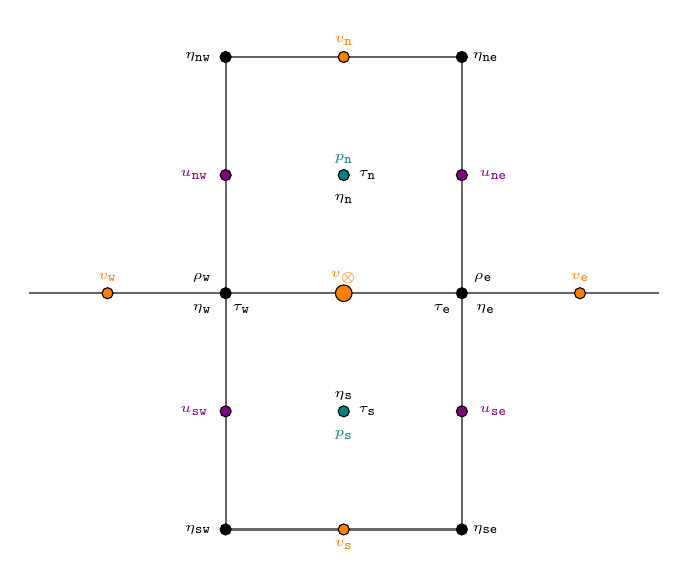
\begin{tikzpicture}
%\draw[fill=gray!23,gray!23](0,0) rectangle (9,8);
%\draw[step=0.5cm,gray,very thin] (0,0) grid (9,8); %background grid
\draw[thick,black!60] (3,1) -- (3,7) -- (6,7) -- (6,1) -- cycle ; 
\draw[thick,black!60] (0.5,4) -- (8.5,4)  ;   
%---------------------------------------------------
\node[] at (4.5,.8) {\tiny \color{orange} $v_{\tt s}$};
\node[] at (4.5,7.2) {\tiny \color{orange} $v_{\tt n}$};
\node[] at (4.5,4.2) {\tiny \color{orange} $v_\otimes$};
\node[] at (1.5,4.2) {\tiny \color{orange} $v_{\tt w}$};
\node[] at (7.5,4.2) {\tiny \color{orange} $v_{\tt e}$};
\draw[black,fill=orange] (4.5,1)   circle (2pt);
\draw[black,fill=orange] (4.5,4)   circle (3pt);
\draw[black,fill=orange] (4.5,7)   circle (2pt);
\draw[black,fill=orange] (1.5,4)   circle (2pt);
\draw[black,fill=orange] (7.5,4)   circle (2pt);
%--------------------------------------------------
\draw[black,fill=violet] (3,2.5)   circle (2pt);
\draw[black,fill=violet] (6,2.5)   circle (2pt);
\draw[black,fill=violet] (3,5.5)   circle (2pt);
\draw[black,fill=violet] (6,5.5)   circle (2pt);
\node[] at (2.6,2.5) {\tiny \color{violet} $u_{\tt sw}$};
\node[] at (6.4,2.5) {\tiny \color{violet} $u_{\tt se}$};
\node[] at (2.6,5.5) {\tiny \color{violet} $u_{\tt nw}$};
\node[] at (6.4,5.5) {\tiny \color{violet} $u_{\tt ne}$};
%-----------------------------------------------
\draw[black,fill=black] (3,1)   circle (2pt); 
\draw[black,fill=black] (3,4)   circle (2pt); 
\draw[black,fill=black] (3,7)   circle (2pt); 
\draw[black,fill=black] (6,1)   circle (2pt); 
\draw[black,fill=black] (6,4)   circle (2pt); 
\draw[black,fill=black] (6,7)   circle (2pt); 
%------------------------------------------------
\draw[black,fill=teal] (4.5,2.5)   circle (2pt);
\draw[black,fill=teal] (4.5,5.5)   circle (2pt);
\node[] at (4.5,2.2) {\tiny \color{teal} $p_{\tt s}$};
\node[] at (4.5,5.7) {\tiny \color{teal} $p_{\tt n}$};
%-----------------------------------------
\node[] at (6.27,4.2) {\tiny $\rho_{\tt e}$};
\node[] at (2.7,4.2) {\tiny $\rho_{\tt w}$};
\node[] at (4.5,5.2) {\tiny $\eta_{\tt n}$};
\node[] at (4.5,2.7) {\tiny $\eta_{\tt s}$};
\node[] at (6.3,1) {\tiny $\eta_{\tt se}$};
\node[] at (2.65,1) {\tiny $\eta_{\tt sw}$};
\node[] at (6.3,7) {\tiny $\eta_{\tt ne}$};
\node[] at (2.65,7) {\tiny $\eta_{\tt nw}$};
\node[] at (6.3,3.8) {\tiny $\eta_{\tt e}$};
\node[] at (2.7,3.8) {\tiny $\eta_{\tt w}$};

\node[] at (3.2,3.8) {\tiny $\tau_{\tt w}$};
\node[] at (5.75,3.8) {\tiny $\tau_{\tt e}$};
\node[] at (4.8,5.5) {\tiny $\tau_{\tt n}$};
\node[] at (4.8,2.5) {\tiny $\tau_{\tt s}$};


\end{tikzpicture}
\end{center}



{\captionfont Node layout in {n-e-w-s} notations.}

\columnbreak

\begin{center}
\includegraphics[width=6.5cm]{images/fdm/gerya_C}\\
\includegraphics[width=7cm]{images/fdm/gerya_E}\\
\includegraphics[width=4.5cm]{images/fdm/gerya_G}\\
{\captionfont Taken from Gerya's book}
\end{center}
\end{multicols}


We start from 
\[
\frac{\partial \tau_{xy}}{\partial x}  + 
\frac{\partial \tau_{yy}}{\partial y}  
- \frac{\partial p}{\partial y} + \rho g_y = 0
\]
which we discretise as follows on the ${\color{orange} v_\otimes}$ node in the middle
\[
\frac{\tau_{xy,{\tt e}}-\tau_{xy,{\tt w}}}{h_x} + \frac{\tau_{yy,{\tt n}}-\tau_{yy,{\tt s}}}{h_y} 
-\frac{{\color{teal}p_{\tt n}}-{\color{teal}p_{\tt s}}}{h_y} 
= -\frac{\rho_{\tt e}+\rho_{\tt w}}{2} g_y
\]
where
\begin{eqnarray}
\tau_{xy,{\tt e}} 
&=& 2 \eta_{\tt e} \dot{\varepsilon}_{xy,{\tt e}} 
= \eta_{\tt e} \left( \frac{{\color{violet} u_{\tt ne}}-{\color{violet} u_{\tt se}}}{h_y} 
+\frac{{\color{orange} v_{\tt e}}-{\color{orange} v_\otimes}}{h_x} \right) 
\nn \\
\tau_{xy,{\tt w}} 
&=& 2 \eta_{\tt w} \dot{\varepsilon}_{xy,{\tt w}} 
= \eta_{\tt w} \left( \frac{{\color{violet} u_{\tt nw}}-{\color{violet} u_{\tt sw}}}{h_y} 
+\frac{{\color{orange} v_\otimes} - {\color{orange} v_{\tt w}}}{h_x} \right) 
\nn\\
\tau_{yy,{\tt n}} 
&=& 2 \eta_{\tt n} \dot{\varepsilon}_{yy,{\tt n}} 
= 2\eta_{\tt n} \frac{{\color{orange} v_{\tt n}}-{\color{orange} v_\otimes}}{h_y} 
\nn\\
\tau_{yy,{\tt s}} 
&=& 2 \eta_{\tt s} \dot{\varepsilon}_{yy,{\tt s}} 
= 2\eta_{\tt s} \frac{{\color{orange} v_\otimes} -{\color{orange} v_{\tt s}}}{h_y} 
 \nn
\end{eqnarray}

Again, we will discuss later in Section~\ref{ss:fdm_stokes_visc} how to arrive at 
$\eta_{\tt n}$ and $\eta_{\tt s}$.
Inserting the four equations above into the first one, we obtain:



\[
\frac{1}{h_x} \left(\tau_{xy,{\tt e}}-\tau_{xy,{\tt w}}\right) + 
\frac{1}{h_y} \left(\tau_{yy,{\tt n}}-\tau_{yy,{\tt s}}\right)
-\frac{1}{h_y} {\color{teal}p_{\tt n}} + \frac{1}{h_y} {\color{teal}p_{\tt s}}
= -\frac{\rho_{\tt e}+\rho_{\tt w}}{2} g_y
\]



{\footnotesize
\[
\frac{1}{h_x} \left[
\eta_{\tt e} \left( \frac{{\color{violet} u_{\tt ne}}-{\color{violet} u_{\tt se}}}{h_y} 
+\frac{{\color{orange} v_{\tt e}}-{\color{orange} v_\otimes}}{h_x} \right) 
-
\eta_{\tt w} \left( \frac{{\color{violet} u_{\tt nw}}-{\color{violet} u_{\tt sw}}}{h_y} 
+\frac{{\color{orange} v_\otimes} - {\color{orange} v_{\tt w}}}{h_x} \right) 
\right] 
+
\frac{1}{h_y} \left(
2\eta_{\tt n} \frac{{\color{orange} v_{\tt n}}-{\color{orange} v_\otimes}}{h_y} 
-
2\eta_{\tt s} \frac{{\color{orange} v_\otimes} -{\color{orange} v_{\tt s}}}{h_y}
\right)
-\frac{1}{h_y} {\color{teal}p_{\tt n}} + \frac{1}{h_y} {\color{teal}p_{\tt s}}
= -\frac{\rho_{\tt e}+\rho_{\tt w}}{2} g_y
\]
}





{\footnotesize
\[
\frac{\eta_{\tt e}}{h_x} 
 \left( \frac{{\color{violet} u_{\tt ne}}-{\color{violet} u_{\tt se}}}{h_y} 
+\frac{{\color{orange} v_{\tt e}}-{\color{orange} v_\otimes}}{h_x} \right) 
-
\frac{\eta_{\tt w}}{h_x} \left( \frac{{\color{violet} u_{\tt nw}}-{\color{violet} u_{\tt sw}}}{h_y} 
+\frac{{\color{orange} v_\otimes} - {\color{orange} v_{\tt w}}}{h_x} \right) 
+
\frac{2\eta_{\tt n}}{h_y} 
 \frac{{\color{orange} v_{\tt n}}-{\color{orange} v_\otimes}}{h_y} 
-
\frac{2\eta_{\tt s}}{h_y}   \frac{{\color{orange} v_\otimes} -{\color{orange} v_{\tt s}}}{h_y}
-\frac{1}{h_y} {\color{teal}p_{\tt n}} + \frac{1}{h_y} {\color{teal}p_{\tt s}}
= -\frac{\rho_{\tt e}+\rho_{\tt w}}{2} g_y
\]
}

\begin{mdframed}[backgroundcolor=blue!5]
\begin{eqnarray}
\left( \frac{2\eta_{\tt n}}{h_y^2} \right) {\color{orange} v_{\tt n}} +
\left( \frac{ \eta_{\tt e}}{h_x^2} \right) {\color{orange} v_{\tt e}} +
\left( \frac{ \eta_{\tt w}}{h_x^2} \right) {\color{orange} v_{\tt w}} +
\left( \frac{2\eta_{\tt s}}{h_y^2} \right) {\color{orange} v_{\tt s}} +
\left( 
-\frac{\eta_{\tt e}}{h_x^2} 
-\frac{\eta_{\tt w}}{h_x^2} 
-\frac{2\eta_{\tt n}}{h_y^2} 
-\frac{2\eta_{\tt s}}{h_y^2} 
\right) {\color{orange} v_\otimes} \nn\\
+
\left( \frac{\eta_{\tt e}}{h_x h_y} \right) {\color{violet} u_{\tt ne}} +
\left(-\frac{\eta_{\tt e}}{h_x h_y} \right) {\color{violet} u_{\tt se}} +
\left(-\frac{\eta_{\tt w}}{h_x h_y} \right) {\color{violet} u_{\tt nw}} +
\left( \frac{\eta_{\tt w}}{h_x h_y} \right) {\color{violet} u_{\tt sw}} 
-\frac{1}{h_y} {\color{teal}p_{\tt n}} + \frac{1}{h_y} {\color{teal}p_{\tt s}}
&=& -\frac{\rho_{\tt e}+\rho_{\tt w}}{2} g_y \nn\\
\label{eq:fdmstokes2}
\end{eqnarray}
\end{mdframed}


%----------------------------------
\subsection{Continuity equation}

In two dimensions the continuity equation for an incompressible flow is
\[
\vec\nabla \cdot \vec\upnu 
= 
\frac{\partial u}{\partial x} 
+
\frac{\partial v}{\partial y} 
=0
\]
We can isolate one cell:

\begin{flushright} {\tiny {\color{gray} (tikz\_staggered2D\_divv.tex)}} \end{flushright}
%~~~~~~~~~~~~~~~~~~~~~~~~~~~~~~~~~~~~~~~~~~~~~~~~~~~~~~~~~~~~~~~~~~~~~~~~~~~~~~~~~~~~~~~~~~~~~~~~~~


\begin{center}
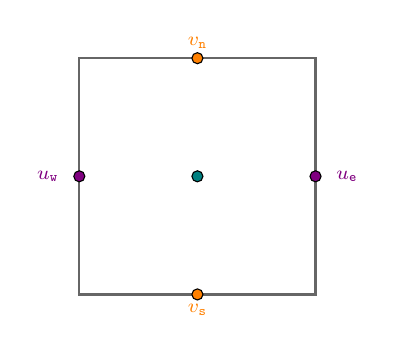
\begin{tikzpicture}
%\draw[fill=gray!23,gray!23](0,0) rectangle (5,5);
%\draw[step=0.5cm,gray,very thin] (0,0) grid (5,5); %background grid
\draw[thick,black!60] (1,1) -- (4,1) -- (4,4) -- (1,4) -- cycle ; 
\draw[black,fill=teal] (2.5,2.5)   circle (2pt);
%---------------------------------------------------
\node[] at (2.5,0.8) {\scriptsize \color{orange} $v_{\tt s}$};
\node[] at (2.5,4.2) {\scriptsize \color{orange} $v_{\tt n}$};
\draw[black,fill=orange] (2.5,1)   circle (2pt);
\draw[black,fill=orange] (2.5,4)   circle (2pt);
%---------------------------------------------------
\node[] at (0.6,2.5) {\scriptsize \color{violet} $u_{\tt w}$};
\node[] at (4.4,2.5) {\scriptsize \color{violet} $u_{\tt e}$};
\draw[black,fill=violet] (1,2.5)   circle (2pt);
\draw[black,fill=violet] (4,2.5)   circle (2pt);
\end{tikzpicture}
\end{center}





and discretise the equation above in its middle.
\begin{mdframed}[backgroundcolor=blue!5]
\begin{equation}
\frac{{\color{violet}u_{\tt e}}-{\color{violet}u_{\tt w}}}{h_x} 
+
\frac{{\color{orange}v_{\tt n}}-{\color{orange}v_{\tt s}}}{h_y} 
=0
\label{eq:fdmstokes3}
\end{equation}
\end{mdframed}



%-------------------------------------------------------------------------
\subsection{Viscosity at the center of cells \label{ss:fdm_stokes_visc} }

Following Gerya, the viscosity in the middle of the cells
can be obtained via averaging (for example arithmetic) of the viscosity values at the corners.

In the case of the $x$-component of the momentum equation:
\[
\eta_{\tt w} = \frac{1}{4}(\eta_{\tt sw}+\eta_{\tt s}+\eta_{\tt n} + \eta_{\tt nw})
\]
\[
\eta_{\tt e} = \frac{1}{4}(\eta_{\tt se}+\eta_{\tt s}+\eta_{\tt n} + \eta_{\tt ne})
\]
In the case of the $y$-component of the momentum equation:
\[
\eta_{\tt n} = \frac{1}{4}(\eta_{\tt w}+\eta_{\tt nw}+\eta_{\tt ne} + \eta_{\tt e})
\]
\[
\eta_{\tt s} = \frac{1}{4}(\eta_{\tt sw}+\eta_{\tt w}+\eta_{\tt e} + \eta_{\tt se})
\]
If harmonic averaging is preferred, then for instance we would have
\[
\eta_{\tt w} = \frac{4}{1/\eta_{\tt sw}+1/\eta_{\tt s}+1/\eta_{\tt n} + 1/\eta_{\tt nw} }
\]


%--------------------------------------------------
\subsection{Boundary conditions}

We start with so-called Dirichlet boundary conditions, i.e. we wish 
to prescribe the value of either velocity components on the boundaries.
For simplicity we will then focus on free slip and no slip boundary conditions.
Free slip b.c. are characterised by a) the normal velocity component on the boundary is zero 
b) the other two components do not change across the boundary (i.e.
zero shear strain rate and shear stresses along the boundary).
No slip b.c. require that all velocity components are zero on the boundary.

Gerya presents in Section 7.4 all the types of boundary conditions but is remarkably elusive 
as to how they should be implemented. Consulting Becker and Kaus, the same conclusion can 
unfortunately be drawn.

Looking at \textcite{hawe65} (1965)
we see that the authors discuss free-slip and no-slip boundary conditions:
\begin{center}
\fbox{\includegraphics[width=9cm]{images/fdm/hawe65b}}
\end{center}
As mentioned in the paper ``a vertical wall therefore passes through the horizontal-velocity mesh points,
and the velocities at those points vanish at all times for either type of [boundary condition].
A vertical wall does not pass through vertical-velocity mesh points, but the calculation makes use
of the values of $v$ at [virtual] mesh points lying just outside of the wall. For a no-slip wall
the boundary condition is $v'=-v$, while for a free-slip wall it becomes $v'=v$ [on the figure above].''

Let us focus on the bottom of the following mesh:
\begin{center}
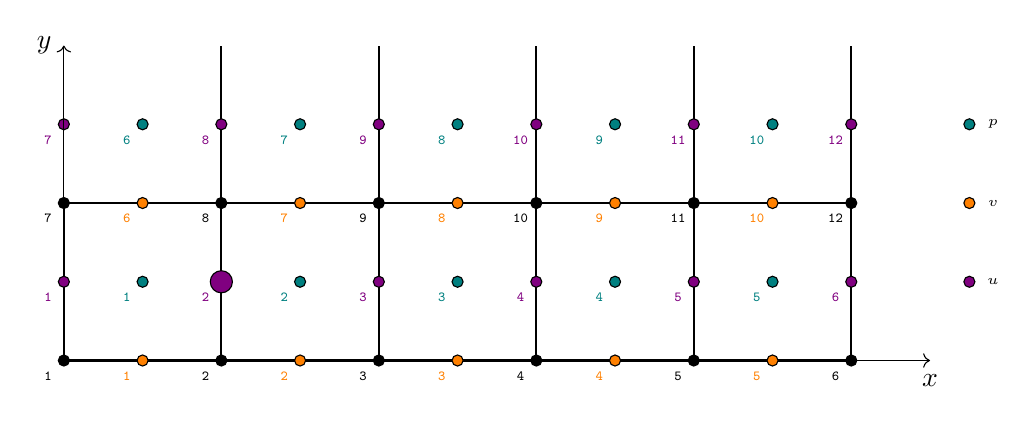
\begin{tikzpicture}
%\draw[fill=gray!23,gray!23](0,0) rectangle (12,10);
%\draw[step=0.5cm,gray,very thin] (0,0) grid (12,10); %background grid

\draw[thick] (0,0) -- (10,0) -- (10,2) -- (0,2) -- cycle ; %1-4
\draw[thick] (0,2) -- (10,2)  ; 
\draw[thick] (2,0) -- (2,4)  ; 
\draw[thick] (4,0) -- (4,4)  ; 
\draw[thick] (6,0) -- (6,4)  ; 
\draw[thick] (8,0) -- (8,4)  ; 
\draw[thick] (10,0) -- (10,4)  ; 
%pressure nodes
\draw[black,fill=teal] (1,1)   circle (2pt); %1
\draw[black,fill=teal] (3,1)   circle (2pt); %1
\draw[black,fill=teal] (5,1)   circle (2pt); %1
\draw[black,fill=teal] (7,1)   circle (2pt); %1
\draw[black,fill=teal] (9,1)   circle (2pt); %1
\draw[black,fill=teal] (1,3)   circle (2pt); %1
\draw[black,fill=teal] (3,3)   circle (2pt); %1
\draw[black,fill=teal] (5,3)   circle (2pt); %1
\draw[black,fill=teal] (7,3)   circle (2pt); %1
\draw[black,fill=teal] (9,3)   circle (2pt); %1
\node[] at (0.8,0.8) {\tiny \color{teal} \tt 1};
\node[] at (2.8,0.8) {\tiny \color{teal} \tt 2};
\node[] at (4.8,0.8) {\tiny \color{teal} \tt 3};
\node[] at (6.8,0.8) {\tiny \color{teal} \tt 4};
\node[] at (8.8,0.8) {\tiny \color{teal} \tt 5};
\node[] at (0.8,2.8) {\tiny \color{teal} \tt 6};
\node[] at (2.8,2.8) {\tiny \color{teal} \tt 7};
\node[] at (4.8,2.8) {\tiny \color{teal} \tt 8};
\node[] at (6.8,2.8) {\tiny \color{teal} \tt 9};
\node[] at (8.8,2.8) {\tiny \color{teal} \tt 10};

% u nodes
\draw[black,fill=violet] (0,1)   circle (2pt); 
\draw[black,fill=violet] (2,1)   circle (4pt); 
\draw[black,fill=violet] (4,1)   circle (2pt); 
\draw[black,fill=violet] (6,1)   circle (2pt); 
\draw[black,fill=violet] (8,1)   circle (2pt); 
\draw[black,fill=violet] (10,1)   circle (2pt);
\draw[black,fill=violet] (0,3)   circle (2pt); 
\draw[black,fill=violet] (2,3)   circle (2pt); 
\draw[black,fill=violet] (4,3)   circle (2pt); 
\draw[black,fill=violet] (6,3)   circle (2pt); 
\draw[black,fill=violet] (8,3)   circle (2pt); 
\draw[black,fill=violet] (10,3)   circle (2pt);


\node[] at (-0.2,0.8) {\tiny \color{violet} \tt 1};
\node[] at (1.8,0.8) {\tiny \color{violet} \tt 2};
\node[] at (3.8,0.8) {\tiny \color{violet} \tt 3};
\node[] at (5.8,0.8) {\tiny \color{violet} \tt 4};
\node[] at (7.8,0.8) {\tiny \color{violet} \tt 5};
\node[] at (9.8,0.8) {\tiny \color{violet} \tt 6};
\node[] at (-0.2,2.8) {\tiny \color{violet} \tt 7};
\node[] at (1.8,2.8) {\tiny \color{violet} \tt 8};
\node[] at (3.8,2.8) {\tiny \color{violet} \tt 9};
\node[] at (5.8,2.8) {\tiny \color{violet} \tt 10};
\node[] at (7.8,2.8) {\tiny \color{violet} \tt 11};
\node[] at (9.8,2.8) {\tiny \color{violet} \tt 12};

% v nodes
\draw[black,fill=orange] (1,0)   circle (2pt); 
\draw[black,fill=orange] (3,0)   circle (2pt); 
\draw[black,fill=orange] (5,0)   circle (2pt); 
\draw[black,fill=orange] (7,0)   circle (2pt); 
\draw[black,fill=orange] (9,0)   circle (2pt); 

\draw[black,fill=orange] (1,2)   circle (2pt); 
\draw[black,fill=orange] (3,2)   circle (2pt); 
\draw[black,fill=orange] (5,2)   circle (2pt); 
\draw[black,fill=orange] (7,2)   circle (2pt); 
\draw[black,fill=orange] (9,2)   circle (2pt); 

\node[] at (0.8,-0.2) {\tiny \color{orange} \tt 1};
\node[] at (2.8,-0.2) {\tiny \color{orange} \tt 2};
\node[] at (4.8,-0.2) {\tiny \color{orange} \tt 3};
\node[] at (6.8,-0.2) {\tiny \color{orange} \tt 4};
\node[] at (8.8,-0.2) {\tiny \color{orange} \tt 5};
\node[] at (0.8,1.8) {\tiny \color{orange} \tt 6};
\node[] at (2.8,1.8) {\tiny \color{orange} \tt 7};
\node[] at (4.8,1.8) {\tiny \color{orange} \tt 8};
\node[] at (6.8,1.8) {\tiny \color{orange} \tt 9};
\node[] at (8.8,1.8) {\tiny \color{orange} \tt 10};
%------------------------------------------------
\draw[black,fill=black] (0,0)   circle (2pt); 
\draw[black,fill=black] (2,0)   circle (2pt); 
\draw[black,fill=black] (4,0)   circle (2pt); 
\draw[black,fill=black] (6,0)   circle (2pt); 
\draw[black,fill=black] (8,0)   circle (2pt); 
\draw[black,fill=black] (10,0)   circle (2pt); 
\draw[black,fill=black] (0,2)   circle (2pt); 
\draw[black,fill=black] (2,2)   circle (2pt); 
\draw[black,fill=black] (4,2)   circle (2pt); 
\draw[black,fill=black] (6,2)   circle (2pt); 
\draw[black,fill=black] (8,2)   circle (2pt); 
\draw[black,fill=black] (10,2)   circle (2pt); 
\node[] at (-0.2,-0.2) {\tiny \tt 1};
\node[] at (1.8,-0.2) {\tiny \tt 2};
\node[] at (3.8,-0.2) {\tiny \tt 3};
\node[] at (5.8,-0.2) {\tiny \tt 4};
\node[] at (7.8,-0.2) {\tiny \tt 5};
\node[] at (9.8,-0.2) {\tiny \tt 6};
\node[] at (-0.2,1.8) {\tiny \tt 7};
\node[] at (1.8,1.8) {\tiny \tt 8};
\node[] at (3.8,1.8) {\tiny \tt 9};
\node[] at (5.8,1.8) {\tiny \tt 10};
\node[] at (7.8,1.8) {\tiny \tt 11};
\node[] at (9.8,1.8) {\tiny \tt 12};
%-------------------------------------------------
\draw[thin,->] (10,0) -- (11,0);  \node[] at (11,-0.25) {$x$};
\draw[thin,->] (0,2) -- (0,4); \node[] at (-0.25,4) {$y$};
%-------------------------------------------------
\draw[black,fill=teal] (11.5,3)   circle (2pt); \node[] at (11.8,3) {\tiny $p$};
\draw[black,fill=orange] (11.5,2)   circle (2pt); \node[] at (11.8,2) {\tiny $v$};
\draw[black,fill=violet] (11.5,1)   circle (2pt); \node[] at (11.8,1) {\tiny $u$};
\end{tikzpicture}
\end{center}



\begin{itemize}
\item \underline{No slip} (at the bottom). We then want $u=v=0$. We can easily zero 
${\color{orange} v_{\tt 1,2,3,4,5}}$ since the corresponding nodes are on the boundary but this is not enough. Let us consider node ${\color{violet}u_{\tt 2}}$ (bigger on the figure above). 
We could zero $u_2$ directly but this would not be correct since the node is not on the boundary.
If we wish to impose $u=0$ exactly on the boundary then its south neighbour ghost value should be set to
-{\color{violet} $u_2$} and used in the established stencils.


\begin{center}
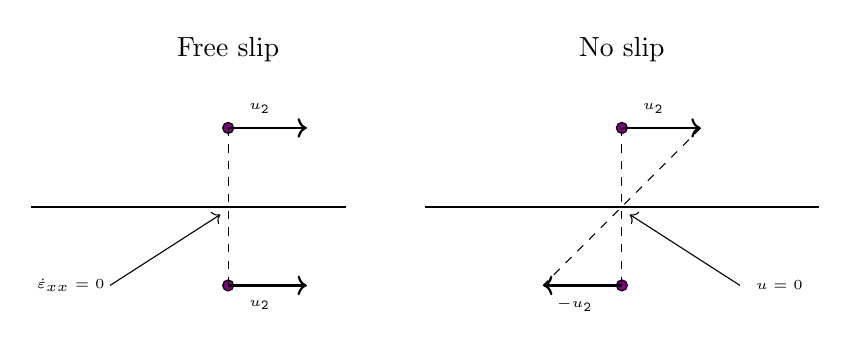
\begin{tikzpicture}
%\draw[fill=gray!23,gray!23](0,0) rectangle (12,6);
%\draw[step=0.5cm,gray,very thin] (0,0) grid (12,6); %background grid
\node[] at (3.5,4) {Free slip};
\node[] at (8.5,4) {No slip};
\draw[thick] (1,2) -- (5,2) ; 
\draw[thick] (6,2) -- (11,2) ; 
\draw[black,fill=violet] (3.5,1)   circle (2pt); 
\draw[black,fill=violet] (3.5,3)   circle (2pt); 
\draw[black,fill=violet] (8.5,1)   circle (2pt); 
\draw[black,fill=violet] (8.5,3)   circle (2pt); 
\draw[dashed] (3.5,1) -- (3.5,3) ; 
\draw[dashed] (8.5,1) -- (8.5,3) ; 
\draw[thin,dashed] (9.5,3) -- (7.5,1) ; 
\draw[thick, ->] (3.5,3)--(4.5,3);
\draw[thick, ->] (3.5,1)--(4.5,1);
\draw[thick, ->] (8.5,3)--(9.5,3);
\draw[thick, ->] (8.5,1)--(7.5,1);
\draw[->] (2,1)--(3.4,1.9);
\node[] at (1.5,1) {\tiny $\dot\varepsilon_{xx}=0$};
\draw[->] (10,1)--(8.6,1.9);
\node[] at (10.5,1) {\tiny $u=0$};

\node[] at (3.9,3.25) {\tiny $u_{\tt 2}$};
\node[] at (3.9,0.75) {\tiny $u_{\tt 2}$};


\node[] at (8.9,3.25) {\tiny $u_{\tt 2}$};
\node[] at (7.9,0.75) {\tiny $-u_{\tt 2}$};

\end{tikzpicture}
\end{center}


\item \underline{Free slip} (at the bottom). Aside from the zero normal velocity 
as above, we also need the tangential velocity gradient to be zero on the boundary, 
which translates into assigning its south neighbour ghost the value +${\color{violet} u_2}$ 
\end{itemize}

We see that in both cases we will need to create ephemeral boundary nodes outside the domain and assign
them specific values based on the boundary condition type. 
This consideration lead Becker \& Kaus to produce this figure in their syllabus:

\begin{center}
\includegraphics[width=8cm]{images/fdm/bk_A}\\
{\captionfont Taken from \textcite{beka}: Staggered grid definition with the boundary points. 
Within the purple domain, the
finite difference scheme for center points can be applied. At the boundaries, we have to apply a
special finite difference scheme which employs fictitious boundary nodes.}
\end{center}

Let us consider a $4\times 3$ mesh.
We have 12 cells, 15 {\color{violet}$u$}-nodes, 
16 {\color{orange}$v$}-nodes and 12 {\color{teal}$p$}-nodes.
This mesh then counts $N=15+16+12=43$ unknowns\footnote{
Note that the numbering starts at zero, python-style.}.

\input{tikz/tikz_staggered2D_4x3}

Let us assume that we prescribe free slip or no slip on all sides.
Then we must set 
${\color{orange}v_{\tt 0}}={\color{orange}v_{\tt 1}}={\color{orange}v_{\tt 2}}={\color{orange}v_{\tt 3}}={\color{orange}v_{\tt 12}}={\color{orange}v_{\tt 13}}={\color{orange}v_{\tt 14}}={\color{orange}v_{\tt 15}}=0$
and ${\color{violet} u_{\tt 0}}={\color{violet}u_{\tt 4}}={\color{violet}u_{\tt 5}}
={\color{violet}u_{\tt 9}}={\color{violet}u_{\tt 10}} = {\color{violet}u_{\tt 14}}=0$.
This means that we need not discretise the momentum equation on these nodes.

Let us consider node ${\color{violet} u_{7}}$. It has four neighbours so the $x$-component of 
the momentum equation writes there:

\begin{eqnarray}
&&
\left( \frac{\eta_{\tt n}}{h_y^2} \right) {\color{violet} u_{\tt 12}} + 
\left( \frac{2\eta_{\tt e}}{h_x^2} \right) {\color{violet} u_{\tt 8}} + 
\left( \frac{2\eta_{\tt w}}{h_x^2} \right) {\color{violet} u_{\tt 5}} + 
\left( \frac{\eta_{\tt s}}{h_y^2} \right) {\color{violet} u_{\tt 2}} + 
\left( -\frac{2\eta_{\tt e}}{h_x^2} -\frac{2\eta_{\tt w}}{h_x^2}  
-\frac{\eta_{\tt n}}{h_y^2} -\frac{\eta_{\tt s}}{h_y^2}  
\right) {\color{violet} u_7} \nn\\
&&+
\left( \frac{\eta_{\tt n}}{h_x h_y} \right) {\color{orange} v_{\tt 10}}+ 
\left(-\frac{\eta_{\tt n}}{h_x h_y} \right) {\color{orange} v_{\tt 9}}+ 
\left(-\frac{\eta_{\tt s}}{h_x h_y} \right) {\color{orange} v_{\tt 6}}+ 
\left( \frac{\eta_{\tt s}}{h_x h_y} \right) {\color{orange} v_{\tt 5}} 
- \frac{1}{h_x} {\color{teal}p_{\tt 6}} + \frac{1}{h_x} {\color{teal}p_{\tt 5}} = -\frac{\rho_{\tt 12}+\rho_{\tt 7}}{2} g_x 
\nn
\end{eqnarray}





Based on the considerations above pertaining to ghost/virtual nodes
we turn once more to our $4\times 3$ cell mesh where ghost/virtual nodes have been added:

\begin{flushright} {\tiny {\color{gray} (tikz\_staggered2D\_4x3.tex)}} \end{flushright}
%~~~~~~~~~~~~~~~~~~~~~~~~~~~~~~~~~~~~~~~~~~~~~~~~~~~~~~~~~~~~~~~~~~~~~~~~~~~~~~~~~~~~~~~~~~~~~~~~~~


\begin{center}
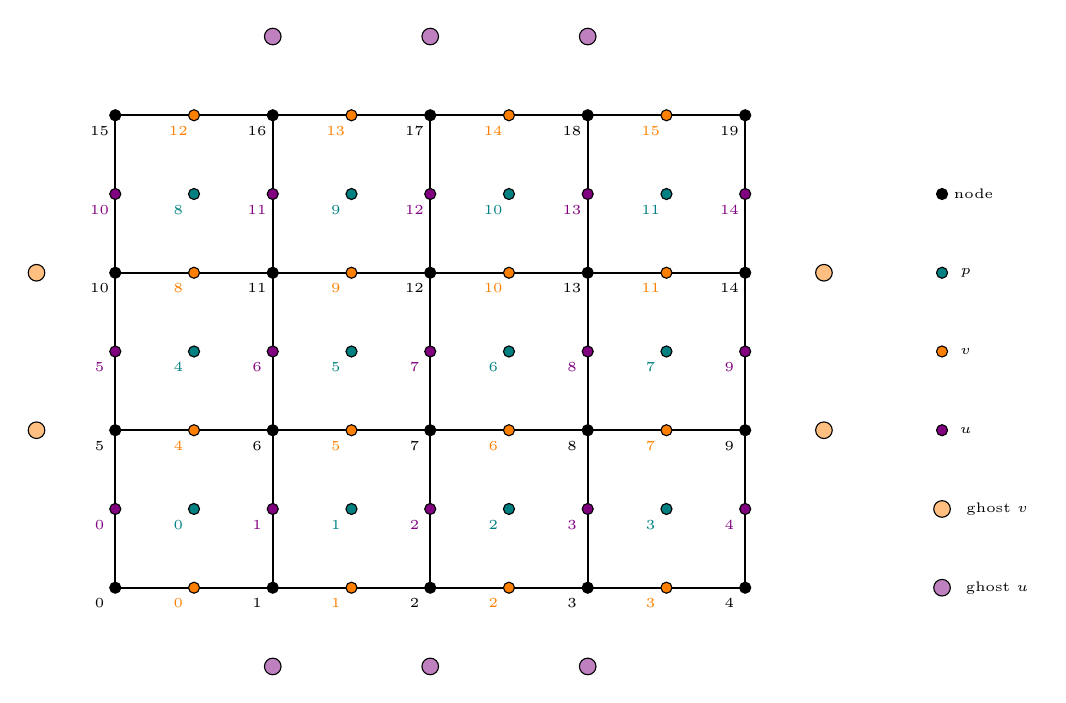
\begin{tikzpicture}
%\draw[fill=gray!23,gray!23](0,0) rectangle (12,10);
%\draw[step=0.5cm,gray,very thin] (0,0) grid (12,10); %background grid

\draw[thick] (0,0) -- (8,0) -- (8,6) -- (0,6) -- cycle ; %1-4
\draw[thick] (0,2) -- (8,2)  ; 
\draw[thick] (0,4) -- (8,4)  ; 
\draw[thick] (2,0) -- (2,6)  ; 
\draw[thick] (4,0) -- (4,6)  ; 
\draw[thick] (6,0) -- (6,6)  ; 

%pressure nodes
\draw[black,fill=teal] (1,1)   circle (2pt); 
\draw[black,fill=teal] (3,1)   circle (2pt); 
\draw[black,fill=teal] (5,1)   circle (2pt); 
\draw[black,fill=teal] (7,1)   circle (2pt); 

\draw[black,fill=teal] (1,3)   circle (2pt); 
\draw[black,fill=teal] (3,3)   circle (2pt); 
\draw[black,fill=teal] (5,3)   circle (2pt); 
\draw[black,fill=teal] (7,3)   circle (2pt); 

\draw[black,fill=teal] (1,5)   circle (2pt); 
\draw[black,fill=teal] (3,5)   circle (2pt); 
\draw[black,fill=teal] (5,5)   circle (2pt); 
\draw[black,fill=teal] (7,5)   circle (2pt); 

\node[] at (0.8,0.8) {\tiny \color{teal} 0};
\node[] at (2.8,0.8) {\tiny \color{teal} 1};
\node[] at (4.8,0.8) {\tiny \color{teal} 2};
\node[] at (6.8,0.8) {\tiny \color{teal} 3};

\node[] at (0.8,2.8) {\tiny \color{teal} 4};
\node[] at (2.8,2.8) {\tiny \color{teal} 5};
\node[] at (4.8,2.8) {\tiny \color{teal} 6};
\node[] at (6.8,2.8) {\tiny \color{teal} 7};

\node[] at (0.8,4.8) {\tiny \color{teal} 8};
\node[] at (2.8,4.8) {\tiny \color{teal} 9};
\node[] at (4.8,4.8) {\tiny \color{teal} 10};
\node[] at (6.8,4.8) {\tiny \color{teal} 11};

% u nodes
\draw[black,fill=violet] (0,1)   circle (2pt); 
\draw[black,fill=violet] (2,1)   circle (2pt); 
\draw[black,fill=violet] (4,1)   circle (2pt); 
\draw[black,fill=violet] (6,1)   circle (2pt); 
\draw[black,fill=violet] (8,1)   circle (2pt); 

\draw[black,fill=violet] (0,3)   circle (2pt); 
\draw[black,fill=violet] (2,3)   circle (2pt); 
\draw[black,fill=violet] (4,3)   circle (2pt); 
\draw[black,fill=violet] (6,3)   circle (2pt);
\draw[black,fill=violet] (8,3)   circle (2pt);

\draw[black,fill=violet] (0,5)   circle (2pt); 
\draw[black,fill=violet] (2,5)   circle (2pt); 
\draw[black,fill=violet] (4,5)   circle (2pt); 
\draw[black,fill=violet] (6,5)   circle (2pt);
\draw[black,fill=violet] (8,5)   circle (2pt);

\node[] at (-0.2,0.8) {\tiny \color{violet} 0};
\node[] at (1.8,0.8)  {\tiny \color{violet} 1};
\node[] at (3.8,0.8)  {\tiny \color{violet} 2};
\node[] at (5.8,0.8)  {\tiny \color{violet} 3};
\node[] at (7.8,0.8)  {\tiny \color{violet} 4};

\node[] at (-0.2,2.8) {\tiny \color{violet} 5};
\node[] at (1.8,2.8)  {\tiny \color{violet} 6};
\node[] at (3.8,2.8)  {\tiny \color{violet} 7};
\node[] at (5.8,2.8)  {\tiny \color{violet} 8};
\node[] at (7.8,2.8)  {\tiny \color{violet} 9};

\node[] at (-0.2,4.8){\tiny \color{violet} 10};
\node[] at (1.8,4.8) {\tiny \color{violet} 11};
\node[] at (3.8,4.8) {\tiny \color{violet} 12};
\node[] at (5.8,4.8) {\tiny \color{violet} 13};
\node[] at (7.8,4.8) {\tiny \color{violet} 14};

% v nodes
\draw[black,fill=orange] (1,0)   circle (2pt); 
\draw[black,fill=orange] (3,0)   circle (2pt); 
\draw[black,fill=orange] (5,0)   circle (2pt); 
\draw[black,fill=orange] (7,0)   circle (2pt); 

\draw[black,fill=orange] (1,2)   circle (2pt); 
\draw[black,fill=orange] (3,2)   circle (2pt); 
\draw[black,fill=orange] (5,2)   circle (2pt); 
\draw[black,fill=orange] (7,2)   circle (2pt); 

\draw[black,fill=orange] (1,4)   circle (2pt); 
\draw[black,fill=orange] (3,4)   circle (2pt); 
\draw[black,fill=orange] (5,4)   circle (2pt); 
\draw[black,fill=orange] (7,4)   circle (2pt); 

\draw[black,fill=orange] (1,6)   circle (2pt); 
\draw[black,fill=orange] (3,6)   circle (2pt); 
\draw[black,fill=orange] (5,6)   circle (2pt); 
\draw[black,fill=orange] (7,6)   circle (2pt); 

\node[] at (0.8,-0.2) {\tiny \color{orange} 0};
\node[] at (2.8,-0.2) {\tiny \color{orange} 1};
\node[] at (4.8,-0.2) {\tiny \color{orange} 2};
\node[] at (6.8,-0.2) {\tiny \color{orange} 3};

\node[] at (0.8,1.8) {\tiny \color{orange} 4};
\node[] at (2.8,1.8) {\tiny \color{orange} 5};
\node[] at (4.8,1.8) {\tiny \color{orange} 6};
\node[] at (6.8,1.8) {\tiny \color{orange} 7};

\node[] at (0.8,3.8) {\tiny \color{orange} 8};
\node[] at (2.8,3.8) {\tiny \color{orange} 9};
\node[] at (4.8,3.8) {\tiny \color{orange} 10};
\node[] at (6.8,3.8) {\tiny \color{orange} 11};

\node[] at (0.8,5.8) {\tiny \color{orange} 12};
\node[] at (2.8,5.8) {\tiny \color{orange} 13};
\node[] at (4.8,5.8) {\tiny \color{orange} 14};
\node[] at (6.8,5.8) {\tiny \color{orange} 15};

%------------------------------------------------

\draw[black,fill=black] (0,0)   circle (2pt); 
\draw[black,fill=black] (2,0)   circle (2pt); 
\draw[black,fill=black] (4,0)   circle (2pt); 
\draw[black,fill=black] (6,0)   circle (2pt); 
\draw[black,fill=black] (8,0)   circle (2pt); 

\draw[black,fill=black] (0,2)   circle (2pt); 
\draw[black,fill=black] (2,2)   circle (2pt); 
\draw[black,fill=black] (4,2)   circle (2pt); 
\draw[black,fill=black] (6,2)   circle (2pt); 
\draw[black,fill=black] (8,2)   circle (2pt); 

\draw[black,fill=black] (0,4)   circle (2pt); 
\draw[black,fill=black] (2,4)   circle (2pt); 
\draw[black,fill=black] (4,4)   circle (2pt); 
\draw[black,fill=black] (6,4)   circle (2pt); 
\draw[black,fill=black] (8,4)   circle (2pt); 

\draw[black,fill=black] (0,6)   circle (2pt); 
\draw[black,fill=black] (2,6)   circle (2pt); 
\draw[black,fill=black] (4,6)   circle (2pt); 
\draw[black,fill=black] (6,6)   circle (2pt); 
\draw[black,fill=black] (8,6)   circle (2pt); 


\node[] at (-0.2,-0.2){\tiny 0};
\node[] at (1.8,-0.2) {\tiny 1};
\node[] at (3.8,-0.2) {\tiny 2};
\node[] at (5.8,-0.2) {\tiny 3};
\node[] at (7.8,-0.2) {\tiny 4};

\node[] at (-0.2,1.8){\tiny 5};
\node[] at (1.8,1.8) {\tiny 6};
\node[] at (3.8,1.8) {\tiny 7};
\node[] at (5.8,1.8) {\tiny 8};
\node[] at (7.8,1.8) {\tiny 9};

\node[] at (-0.2,3.8){\tiny 10};
\node[] at (1.8,3.8) {\tiny 11};
\node[] at (3.8,3.8) {\tiny 12};
\node[] at (5.8,3.8) {\tiny 13};
\node[] at (7.8,3.8) {\tiny 14};

\node[] at (-0.2,5.8){\tiny 15};
\node[] at (1.8,5.8) {\tiny 16};
\node[] at (3.8,5.8) {\tiny 17};
\node[] at (5.8,5.8) {\tiny 18};
\node[] at (7.8,5.8) {\tiny 19};

%-------------------------------------------------

\draw[black,fill=black]  (10.5,5)   circle (2pt); \node[] at (10.9,5) {\tiny node};
\draw[black,fill=teal]   (10.5,4)   circle (2pt); \node[] at (10.8,4) {\tiny $p$};
\draw[black,fill=orange] (10.5,3)   circle (2pt); \node[] at (10.8,3) {\tiny $v$};
\draw[black,fill=violet] (10.5,2)   circle (2pt); \node[] at (10.8,2) {\tiny $u$};

\draw[black,fill=orange!50] (10.5,1)  circle (3pt); \node[] at (11.2,1) {\tiny ghost $v$};
\draw[black,fill=violet!50] (10.5,0)  circle (3pt); \node[] at (11.2,0) {\tiny ghost $u$};

%boundary u nodes
\draw[black,fill=violet!50] (2,-1)   circle (3pt); 
\draw[black,fill=violet!50] (4,-1)   circle (3pt); 
\draw[black,fill=violet!50] (6,-1)   circle (3pt); 
\draw[black,fill=violet!50] (2,7)   circle (3pt); 
\draw[black,fill=violet!50] (4,7)   circle (3pt); 
\draw[black,fill=violet!50] (6,7)   circle (3pt); 

%boundary u nodes
\draw[black,fill=orange!50] (-1,2)   circle (3pt); 
\draw[black,fill=orange!50] (-1,4)   circle (3pt); 
\draw[black,fill=orange!50] (9,2)   circle (3pt); 
\draw[black,fill=orange!50] (9,4)   circle (3pt); 





\end{tikzpicture}
\end{center}



\begin{itemize}
\item ${\color{violet} u_{\tt 0,5,10}}$: situated on left boundary. Free slip and no slip require ${\color{violet} u}=0$. No need for a ghost node.
\item ${\color{violet} u_{\tt 4,9,14}}$: situated on right boundary. Free slip and no slip require ${\color{violet} u}=0$. No need for a ghost node.
\item ${\color{violet} u_{\tt 1,2,3}}$: north, east, west neighbours are present, but south is missing so south ghost nodes are needed.

Let us write the stencil for these nodes:
\begin{eqnarray}
\left( \frac{\eta_{\tt n}}{h_y^2} \right) {\color{violet} u_{\tt n}} + 
\left( \frac{2\eta_{\tt e}}{h_x^2} \right) {\color{violet} u_{\tt e}} + 
\left( \frac{2\eta_{\tt w}}{h_x^2} \right) {\color{violet} u_{\tt w}} + 
\boxed{\left( \frac{\eta_{\tt s}}{h_y^2} \right) {\color{violet} u_{\tt s}}} + 
\left( -\frac{2\eta_{\tt e}}{h_x^2} -\frac{2\eta_{\tt w}}{h_x^2}  
-\frac{\eta_{\tt n}}{h_y^2} -\frac{\eta_{\tt s}}{h_y^2}  
\right) {\color{violet} u_\otimes} \nn\\
+
\left( \frac{\eta_{\tt n}}{h_x h_y} \right) {\color{orange} v_{\tt ne}}+ 
\left(-\frac{\eta_{\tt n}}{h_x h_y} \right) {\color{orange} v_{\tt nw}}+ 
\left(-\frac{\eta_{\tt s}}{h_x h_y} \right) {\color{orange} v_{\tt se}}+ 
\left( \frac{\eta_{\tt s}}{h_x h_y} \right) {\color{orange} v_{\tt sw}} 
- \frac{1}{h_x} {\color{teal}p_{\tt e}} + \frac{1}{h_x} {\color{teal}p_{\tt w}} 
&=& -\frac{\rho_{\tt n}+\rho_{\tt s}}{2} g_x \nn
\end{eqnarray}
As we have seen earlier there is obviously a problem as ${\color{violet} u_{\tt s}}$ (the boxed term)
is not defined.
If we wish to prescribe free slip, we have seen that we must set 
${\color{violet} u_{\tt s}}={\color{violet} u_\otimes}$.
If we wish to prescribe no slip, we have seen that we must set 
${\color{violet} u_{\tt s}}=-{\color{violet} u_\otimes}$.
The stencil then becomes:
\begin{eqnarray}
\left( \frac{\eta_{\tt n}}{h_y^2} \right) {\color{violet} u_{\tt n}} + 
\left( \frac{2\eta_{\tt e}}{h_x^2} \right) {\color{violet} u_{\tt e}} + 
\left( \frac{2\eta_{\tt w}}{h_x^2} \right) {\color{violet} u_{\tt w}} + 
\left( -\frac{2\eta_{\tt e}}{h_x^2} -\frac{2\eta_{\tt w}}{h_x^2}  
-\frac{\eta_{\tt n}}{h_y^2} -(1-\delta_{bc})\frac{\eta_{\tt s}}{h_y^2}
\right) {\color{violet} u_\otimes} \nn\\
+
\left( \frac{\eta_{\tt n}}{h_x h_y} \right) {\color{orange} v_{\tt ne}}+ 
\left(-\frac{\eta_{\tt n}}{h_x h_y} \right) {\color{orange} v_{\tt nw}}+ 
\left(-\frac{\eta_{\tt s}}{h_x h_y} \right) {\color{orange} v_{\tt se}}+ 
\left( \frac{\eta_{\tt s}}{h_x h_y} \right) {\color{orange} v_{\tt sw}} 
- \frac{1}{h_x} {\color{teal}p_{\tt e}} + \frac{1}{h_x} {\color{teal}p_{\tt w}} 
&=& -\frac{\rho_{\tt n}+\rho_{\tt s}}{2} g_x \nn
\end{eqnarray}
where $\delta_{bc}=1$ (free slip) or -1 (no slip).



\item ${\color{violet} u_{\tt 11,12,13}}$: south, east, west neighbours are present, but north is missing so north ghost nodes are needed.

Let us write the stencil for these nodes:
\begin{eqnarray}
\boxed{\left( \frac{\eta_{\tt n}}{h_y^2} \right) {\color{violet} u_{\tt n}}} + 
\left( \frac{2\eta_{\tt e}}{h_x^2} \right) {\color{violet} u_{\tt e}} + 
\left( \frac{2\eta_{\tt w}}{h_x^2} \right) {\color{violet} u_{\tt w}} + 
\left( \frac{\eta_{\tt s}}{h_y^2} \right) {\color{violet} u_{\tt s}} + 
\left( -\frac{2\eta_{\tt e}}{h_x^2} -\frac{2\eta_{\tt w}}{h_x^2}  
-\frac{\eta_{\tt n}}{h_y^2} -\frac{\eta_{\tt s}}{h_y^2}  
\right) {\color{violet} u_\otimes} \nn\\
+
\left( \frac{\eta_{\tt n}}{h_x h_y} \right) {\color{orange} v_{\tt ne}}+ 
\left(-\frac{\eta_{\tt n}}{h_x h_y} \right) {\color{orange} v_{\tt nw}}+ 
\left(-\frac{\eta_{\tt s}}{h_x h_y} \right) {\color{orange} v_{\tt se}}+ 
\left( \frac{\eta_{\tt s}}{h_x h_y} \right) {\color{orange} v_{\tt sw}} 
- \frac{1}{h_x} {\color{teal}p_{\tt e}} + \frac{1}{h_x} {\color{teal}p_{\tt w}} 
&=& -\frac{\rho_{\tt n}+\rho_{\tt s}}{2} g_x \nn
\end{eqnarray}
Here again there is obviously a problem as ${\color{violet} u_{\tt n}}$ is not defined (boxed term).
Using the same $\delta_{bc}$ parameter the stencil then becomes:
\begin{eqnarray}
\left( \frac{2\eta_{\tt e}}{h_x^2} \right) {\color{violet} u_{\tt e}} + 
\left( \frac{2\eta_{\tt w}}{h_x^2} \right) {\color{violet} u_{\tt w}} + 
\left( \frac{\eta_{\tt s}}{h_y^2} \right) {\color{violet} u_{\tt s}} + 
\left( -\frac{2\eta_{\tt e}}{h_x^2} -\frac{2\eta_{\tt w}}{h_x^2}  
-(1-\delta_{bc})\frac{\eta_{\tt n}}{h_y^2} -\frac{\eta_{\tt s}}{h_y^2}  
\right) {\color{violet} u_\otimes} \nn\\
+
\left( \frac{\eta_{\tt n}}{h_x h_y} \right) {\color{orange} v_{\tt ne}}+ 
\left(-\frac{\eta_{\tt n}}{h_x h_y} \right) {\color{orange} v_{\tt nw}}+ 
\left(-\frac{\eta_{\tt s}}{h_x h_y} \right) {\color{orange} v_{\tt se}}+ 
\left( \frac{\eta_{\tt s}}{h_x h_y} \right) {\color{orange} v_{\tt sw}} 
- \frac{1}{h_x} {\color{teal}p_{\tt e}} + \frac{1}{h_x} {\color{teal}p_{\tt w}} 
&=& -\frac{\rho_{\tt n}+\rho_{\tt s}}{2} g_x \nn
\end{eqnarray}



\item ${\color{violet} u_{\tt 6,7,8}}$: standard stencil applies as 
these nodes have four `real' neighbours.
\item ${\color{orange} v_{\tt 0,1,2,3}}$: situated on bottom boundary. Free slip and no slip require ${\color{orange} v}=0$. No need for a ghost node.
\item ${\color{orange} v_{\tt 12,13,14,15}}$: situated on top boundary. Free slip and no slip require ${\color{orange} v}=0$. No need for a ghost node.

\item ${\color{orange} v_{\tt 4,8}}$: north, east, south neighbours are present, but west is missing so west ghost nodes are needed.
\begin{eqnarray}
\left( \frac{2\eta_{\tt n}}{h_y^2} \right) {\color{orange} v_{\tt n}} +
\left( \frac{ \eta_{\tt e}}{h_x^2} \right) {\color{orange} v_{\tt e}} +
\boxed{\left( \frac{ \eta_{\tt w}}{h_x^2} \right) {\color{orange} v_{\tt w}}} +
\left( \frac{2\eta_{\tt s}}{h_y^2} \right) {\color{orange} v_{\tt s}} +
\left( 
-\frac{\eta_{\tt e}}{h_x^2} 
-\frac{\eta_{\tt w}}{h_x^2} 
-\frac{2\eta_{\tt n}}{h_y^2} 
-\frac{2\eta_{\tt s}}{h_y^2} 
\right) {\color{orange} v_\otimes} \nn\\
+
\left( \frac{\eta_{\tt e}}{h_x h_y} \right) {\color{violet} u_{\tt ne}} +
\left(-\frac{\eta_{\tt e}}{h_x h_y} \right) {\color{violet} u_{\tt se}} +
\left(-\frac{\eta_{\tt w}}{h_x h_y} \right) {\color{violet} u_{\tt nw}} +
\left( \frac{\eta_{\tt w}}{h_x h_y} \right) {\color{violet} u_{\tt sw}} 
-\frac{1}{h_y} {\color{teal}p_{\tt n}} + \frac{1}{h_y} {\color{teal}p_{\tt s}}
&=& -\frac{\rho_{\tt e}+\rho_{\tt w}}{2} g_y \nn
\end{eqnarray}
leads to
\begin{eqnarray}
\left( \frac{2\eta_{\tt n}}{h_y^2} \right) {\color{orange} v_{\tt n}} +
\left( \frac{ \eta_{\tt e}}{h_x^2} \right) {\color{orange} v_{\tt e}} +
\left( \frac{2\eta_{\tt s}}{h_y^2} \right) {\color{orange} v_{\tt s}} +
\left( 
-\frac{\eta_{\tt e}}{h_x^2} 
-(1-\delta_{bc})\frac{\eta_{\tt w}}{h_x^2} 
-\frac{2\eta_{\tt n}}{h_y^2} 
-\frac{2\eta_{\tt s}}{h_y^2} 
\right) {\color{orange} v_\otimes} \nn\\
+
\left( \frac{\eta_{\tt e}}{h_x h_y} \right) {\color{violet} u_{\tt ne}} +
\left(-\frac{\eta_{\tt e}}{h_x h_y} \right) {\color{violet} u_{\tt se}} +
\left(-\frac{\eta_{\tt w}}{h_x h_y} \right) {\color{violet} u_{\tt nw}} +
\left( \frac{\eta_{\tt w}}{h_x h_y} \right) {\color{violet} u_{\tt sw}} 
-\frac{1}{h_y} {\color{teal}p_{\tt n}} + \frac{1}{h_y} {\color{teal}p_{\tt s}}
&=& -\frac{\rho_{\tt e}+\rho_{\tt w}}{2} g_y \nn
\end{eqnarray}



\item ${\color{orange} v_{\tt 7,11}}$: south,  west, north neighbours are present, but east is missing so east ghost nodes are needed.
\begin{eqnarray}
\left( \frac{2\eta_{\tt n}}{h_y^2} \right) {\color{orange} v_{\tt n}} +
\boxed{\left( \frac{ \eta_{\tt e}}{h_x^2} \right) {\color{orange} v_{\tt e}}} +
\left( \frac{ \eta_{\tt w}}{h_x^2} \right) {\color{orange} v_{\tt w}} +
\left( \frac{2\eta_{\tt s}}{h_y^2} \right) {\color{orange} v_{\tt s}} +
\left( 
-\frac{\eta_{\tt e}}{h_x^2} 
-\frac{\eta_{\tt w}}{h_x^2} 
-\frac{2\eta_{\tt n}}{h_y^2} 
-\frac{2\eta_{\tt s}}{h_y^2} 
\right) {\color{orange} v_\otimes} \nn\\
+
\left( \frac{\eta_{\tt e}}{h_x h_y} \right) {\color{violet} u_{\tt ne}} +
\left(-\frac{\eta_{\tt e}}{h_x h_y} \right) {\color{violet} u_{\tt se}} +
\left(-\frac{\eta_{\tt w}}{h_x h_y} \right) {\color{violet} u_{\tt nw}} +
\left( \frac{\eta_{\tt w}}{h_x h_y} \right) {\color{violet} u_{\tt sw}} 
-\frac{1}{h_y} {\color{teal}p_{\tt n}} + \frac{1}{h_y} {\color{teal}p_{\tt s}}
&=& -\frac{\rho_{\tt e}+\rho_{\tt w}}{2} g_y \nn
\end{eqnarray}
leads to
\begin{eqnarray}
\left( \frac{2\eta_{\tt n}}{h_y^2} \right) {\color{orange} v_{\tt n}} +
\left( \frac{ \eta_{\tt w}}{h_x^2} \right) {\color{orange} v_{\tt w}} +
\left( \frac{2\eta_{\tt s}}{h_y^2} \right) {\color{orange} v_{\tt s}} +
\left( 
-(1-\delta_{bc})\frac{\eta_{\tt e}}{h_x^2} 
-\frac{\eta_{\tt w}}{h_x^2} 
-\frac{2\eta_{\tt n}}{h_y^2} 
-\frac{2\eta_{\tt s}}{h_y^2} 
\right) {\color{orange} v_\otimes} \nn\\
+
\left( \frac{\eta_{\tt e}}{h_x h_y} \right) {\color{violet} u_{\tt ne}} +
\left(-\frac{\eta_{\tt e}}{h_x h_y} \right) {\color{violet} u_{\tt se}} +
\left(-\frac{\eta_{\tt w}}{h_x h_y} \right) {\color{violet} u_{\tt nw}} +
\left( \frac{\eta_{\tt w}}{h_x h_y} \right) {\color{violet} u_{\tt sw}} 
-\frac{1}{h_y} {\color{teal}p_{\tt n}} + \frac{1}{h_y} {\color{teal}p_{\tt s}}
&=& -\frac{\rho_{\tt e}+\rho_{\tt w}}{2} g_y \nn
\end{eqnarray}


\item ${\color{orange} v_{\tt 5,6,9,10}}$: standard stencil applies as these nodes have four 'real' neighbours.
\item pressure nodes are situated inside each cell and are unaffected by the type of boundary conditions
since the stencil of the continuity equation is always complete (no need for ghost nodes).
\end{itemize}

Note that if free slip or no slip boundary conditions are prescribed on all four boundaries the 
pressure solution is only known up to a constant. Often this pressure nullspace is removed 
from the solution since most solvers will happily solve the linear system even though it is not 
strictly definite. Gerya advocates to set a zero boundary condition on a node (and then re-normalise the 
pressure).

In practice ghost nodes are never created or used. They are useful in order to 
establish the corrected stencils but are entirely absent from the coding.

%---------------------------------------------------
\subsection{Generating the linear system}

Let us now create the vector $\vec{X}$ that is $N=N_u+N_v+N_p=43$ long 
(still considering 
the $4\times 3$ cell mesh presented above):
\[
\vec{X}^T=(\vec{\cal U}, \vec{\cal V}, \vec{\cal P} )=(
u_{\tt \color{violet} 0},u_{\tt \color{violet} 1}, \dots , u_{\tt \color{violet} 14},
v_{\tt \color{orange} 0},v_{\tt \color{orange} 1}, \dots , v_{\tt \color{orange} 15},
p_{\tt \color{teal} 0},p_{\tt \color{teal} 1}, \dots, p_{\tt \color{teal} 11})
\]
We have 14 boundary conditions and 29 stencil equations that establish relationships between 
unknowns  (see previous section) which we can write altogether as a linear system.

The boundary condition $u_{\color{violet} \tt 0}=0$ can be written 
\[
(1,0,0,0,...,0) \cdot \vec{X} = (0,....)^T
\]
so that the lhs horizontal vector becomes the first line of the matrix and we
must write zero in the first element of the rhs vector. 

Likewise the boundary condition $u_{\color{violet} \tt 4}=0$ can be written
\[
(0,0,0,0,1,...,0) \cdot \vec{X} = (.,.,.,.,0,....)^T
\]
and the lhs horizontal vector becomes the 5th line of the matrix and we
must write zero in the 5th element of the rhs vector. 

We repeat this procedure for all $u$ boundary conditions, which allows us to fill 
the 1st, 5th, 6th, 10th, 11th and 14th line of the matrix.

Likewise the boundary conditions on $v$ will yield similar lines in the matrix, 
only the corresponding lines are below the 15 first ones corresponding to $u$.

Considering node ${\color{violet} u_7}$, the stencil equation \eqref{eq:fdmstokes1} then becomes:



\begin{eqnarray}
\left( \frac{\eta_{\tt n}}{h_y^2} \right) {\color{violet} u_{\tt 12}} + 
\left( \frac{2\eta_{\tt e}}{h_x^2} \right) {\color{violet} u_{\tt 8}} + 
\left( \frac{2\eta_{\tt w}}{h_x^2} \right) {\color{violet} u_{\tt 6}} + 
\left( \frac{\eta_{\tt s}}{h_y^2} \right) {\color{violet} u_{\tt 2}} + 
\left( -\frac{2\eta_{\tt e}}{h_x^2} -\frac{2\eta_{\tt w}}{h_x^2}  
-\frac{\eta_{\tt n}}{h_y^2} -\frac{\eta_{\tt s}}{h_y^2}  
\right) {\color{violet} u_7} \nn\\
+
\left( \frac{\eta_{\tt n}}{h_x h_y} \right) {\color{orange} v_{\tt 10}}+ 
\left(-\frac{\eta_{\tt n}}{h_x h_y} \right) {\color{orange} v_{\tt 9}}+ 
\left(-\frac{\eta_{\tt s}}{h_x h_y} \right) {\color{orange} v_{\tt 6}}+ 
\left( \frac{\eta_{\tt s}}{h_x h_y} \right) {\color{orange} v_{\tt 5}} 
- \frac{1}{h_x} {\color{teal}p_{\tt 6}} + \frac{1}{h_x} {\color{teal}p_{\tt 5}} 
&=& -\frac{\rho_{\tt 12}+\rho_{\tt 7}}{2} g_x \nn
\end{eqnarray}
which will correspond to the 7th line in the matrix. The coefficients inside the 
parentheses will be input in the column corresponding to the unknowns they front. 



Because of how the $\vec{X}$ vector is built (first ${\color{violet} u}$, 
then ${\color{orange}v}$ then ${\color{teal} p}$ unknowns)
the resulting linear system takes the following form:
\begin{equation}
\left(
\begin{array}{ccc}
\K_{xx} & \K_{xy} & \G_x \\
\K_{yx} & \K_{yy} & \G_y \\
\Q_x & \Q_y & 0
\end{array}
\right)
\cdot
\vec{X}
=\vec{b}
\label{eq:fdmstokes6}
\end{equation}











%--------------------------------------------------
\subsection{A remark about scaling of terms}

The coefficients before the velocity components are all of the form 
$\eta/h^2$ while those in front of the pressure terms are of the form 
$1/h$. 

In geodynamics typical velocities are of the order of a cm/year, or about 
$10^{-10}$ m/s
while typical pressures are on the order of 1 GPa.
For a viscosity of about $10^{21}$Pa, and a mesh size of about 1km, 
we have:
\[
\frac{\eta}{h^2} v \sim \frac{10^{21}}{1000^2} 10^{-10} \sim 10^6
\]
while
\[
\frac{p}{h} \sim \frac{10^9}{1000} = 10^6
\]
All is fine until we realise that the terms $\eta/h^2$ and $1/h$ 
will form the entries of the matrix, with 
$\eta/h^2 \sim 10^{15}$ and $1/h \sim 10^{-3}$. 
These numbers are more than 10 orders of magnitude appart and will lead to 
numerical inaccuracies inside solvers (direct or iterative). 
It is therefore common\footnote{See entry on the same topic
in the FEM section.} to define ${p}^\star=\frac{L_{ref}}{\eta_{ref}} p$ so that 
for example the $y$-momentum equation stencil becomes


\begin{eqnarray}
\left( \frac{2\eta_{\tt n}}{h_y^2} \right) {\color{orange} v_{\tt n}} +
\left( \frac{ \eta_{\tt e}}{h_x^2} \right) {\color{orange} v_{\tt e}} +
\left( \frac{ \eta_{\tt w}}{h_x^2} \right) {\color{orange} v_{\tt w}} +
\left( \frac{2\eta_{\tt s}}{h_y^2} \right) {\color{orange} v_{\tt s}} +
\left( 
-\frac{\eta_{\tt e}}{h_x^2} 
-\frac{\eta_{\tt w}}{h_x^2} 
-\frac{2\eta_{\tt n}}{h_y^2} 
-\frac{2\eta_{\tt s}}{h_y^2} 
\right) {\color{orange} v_\otimes} \nn\\
+
\left( \frac{\eta_{\tt e}}{h_x h_y} \right) {\color{violet} u_{\tt ne}} +
\left(-\frac{\eta_{\tt e}}{h_x h_y} \right) {\color{violet} u_{\tt se}} +
\left(-\frac{\eta_{\tt w}}{h_x h_y} \right) {\color{violet} u_{\tt nw}} +
\left( \frac{\eta_{\tt w}}{h_x h_y} \right) {\color{violet} u_{\tt sw}} 
-\frac{1}{h_y}\frac{\eta_{ref}}{L_{ref}} {\color{teal} {p}_{\tt n}^\star} 
+\frac{1}{h_y}\frac{\eta_{ref}}{L_{ref}} {\color{teal} {p}_{\tt s}^\star}
&=& -\frac{\rho_{\tt e}+\rho_{\tt w}}{2} g_y \nn
\end{eqnarray}
By appropriately choosing the reference viscosity $\eta_{ref}$ and the reference
length $L_{ref}$ we thereby ensure that the 
resulting matrix contains coefficients which are all only a 
few orders of magnitude apart (reflecting the viscosity range in the domain).

In the end the linear system will take the form 

\begin{equation}
\left(
\begin{array}{ccc}
\K_{xx} & \K_{xy} & \frac{\eta_{ref}}{L_{ref}} \G_x \\
\K_{yx} & \K_{yy} & \frac{\eta_{ref}}{L_{ref}} \G_y \\
\frac{\eta_{ref}}{L_{ref}} \Q_x & \frac{\eta_{ref}}{L_{ref}} \Q_y & 0
\end{array}
\right)
\cdot
\left(
\begin{array}{c}
\vec{\cal U} \\
\vec{\cal V} \\
\vec{\cal P}^\star
\end{array}
\right)
=
\left(
\begin{array}{c}
\vec{b}_x \\
\vec{b}_y \\
\vec{0}
\end{array}
\right)
\label{eq:fdmstokes7}
\end{equation}


















%--------------------------------------------------
\subsection{Making matrix symmetric again}

Looking at Eq.~\eqref{eq:fdmstokes6} we see that the matrix is 
not structurally symmetric. In other words $\K_{xy} \neq \K_{yx}$, 
$\Q_x \neq \G_x^T$, and $\Q_y \neq \G_y^T$, which is obvious only 
looking at the non zero terms on the figures above. 

This stems from how boundary conditions are applied. So far the matrix 
is being built line by line.
Each line corresponding to a node which value is prescribed on the 
boundary receives a 1 on the diagonal and the required value 
(often simply zero) in the rhs.

This is for example happening on the line corresponding to node 
${\color{violet} u_{10}}$. 
But if we then turn to node ${\color{violet} u_{11}}$, the stencil 
equation on this node reads

\begin{eqnarray}
\left( \frac{\eta_{\tt n}}{h_y^2} \right) {\color{violet} u_{\tt n}} + 
\left( \frac{2\eta_{\tt e}}{h_x^2} \right) {\color{violet} u_{\tt 12}} + 
\left( \frac{2\eta_{\tt w}}{h_x^2} \right) {\color{violet} u_{\tt 10}} + 
\left( \frac{\eta_{\tt s}}{h_y^2} \right) {\color{violet} u_{\tt 6}} + 
\left( -\frac{2\eta_{\tt e}}{h_x^2} -\frac{2\eta_{\tt w}}{h_x^2}  
-\frac{\eta_{\tt n}}{h_y^2} -\frac{\eta_{\tt s}}{h_y^2}  
\right) {\color{violet} u_{11}} \nn\\
+
\left( \frac{\eta_{\tt n}}{h_x h_y} \right) {\color{orange} v_{\tt 13}}+ 
\left(-\frac{\eta_{\tt n}}{h_x h_y} \right) {\color{orange} v_{\tt 12}}+ 
\left(-\frac{\eta_{\tt s}}{h_x h_y} \right) {\color{orange} v_{\tt 9}}+ 
\left( \frac{\eta_{\tt s}}{h_x h_y} \right) {\color{orange} v_{\tt 8}} 
- \frac{1}{h_x} {\color{teal}p_{\tt 9}} + \frac{1}{h_x} {\color{teal}p_{\tt 8}} 
&=& -\frac{\rho_{\tt 16}+\rho_{\tt 11}}{2} g_x \nn
\end{eqnarray}

We have of course already seen how to deal with the missing north node which has us write 
\begin{eqnarray}
\left( \frac{2\eta_{\tt e}}{h_x^2} \right) {\color{violet} u_{\tt 12}} + 
\boxed{\left( \frac{2\eta_{\tt w}}{h_x^2} \right) {\color{violet} u_{\tt 10}}} + 
\left( \frac{\eta_{\tt s}}{h_y^2} \right) {\color{violet} u_{\tt 6}} + 
\left( -\frac{2\eta_{\tt e}}{h_x^2} -\frac{2\eta_{\tt w}}{h_x^2}  
-(1-\delta_{bc})\frac{\eta_{\tt n}}{h_y^2} -\frac{\eta_{\tt s}}{h_y^2}  
\right) {\color{violet} u_{11}} \nn\\
+
\boxed{\left( \frac{\eta_{\tt n}}{h_x h_y} \right) {\color{orange} v_{\tt 13}}}+ 
\boxed{\left(-\frac{\eta_{\tt n}}{h_x h_y} \right) {\color{orange} v_{\tt 12}}}+ 
\left(-\frac{\eta_{\tt s}}{h_x h_y} \right) {\color{orange} v_{\tt 9}}+ 
\left( \frac{\eta_{\tt s}}{h_x h_y} \right) {\color{orange} v_{\tt 8}} 
- \frac{1}{h_x} {\color{teal}p_{\tt 9}} + \frac{1}{h_x} {\color{teal}p_{\tt 8}} 
&=& -\frac{\rho_{\tt 16}+\rho_{\tt 11}}{2} g_x \nn
\end{eqnarray}
However, the boxed terms above are {\it also} on the boundary, which means that the 
values of ${\color{violet} u_{\tt 10}}$, ${\color{orange} v_{\tt 12}}$ and ${\color{orange} v_{\tt 13}}$ are known (typically zero).
As such these two terms should make their way to the right hand side, thereby removing entries in 
the matrix and re-establishing the symmetry of the matrix.
Note that it is not wrong to leave these entries, they just do not serve any real purpose. 


\newpage
%------------------------------------------------------------------------
\subsection{Recovering the strain rate tensor from the velocity solution}

Having obtained the velocity field inside the domain we may now 
wish to compute the components of the strain rate tensor, either
for plotting purposes or because (for example) the effective viscosity 
depends on it.

If the Particle-In-Cell technique is used the strain rate needs to 
be computed on each particle. 
{\color{red} how to FDM people do this?}

If it is for plotting purposes, a quick look 
at the the discretisation of the continuity equation tells us that
we know how to compute 
$\dot{\varepsilon}_{xx}=\partial u/ \partial x$ and
$\dot{\varepsilon}_{yy}=\partial v/ \partial y$ in the middle of each cell. 
But quid of $\dot{\varepsilon}_{xy}$ ?

Let us put the two node layouts we have used previously 
in the context of the $x$- and $y$-momentum equation:

\begin{multicols}{2}

\begin{flushright} {\tiny {\color{gray} (tikz\_staggered2D\_u.tex)}} \end{flushright}
%~~~~~~~~~~~~~~~~~~~~~~~~~~~~~~~~~~~~~~~~~~~~~~~~~~~~~~~~~~~~~~~~~~~~~~~~~~~~~~~~~~~~~~~~~~~~~~~~~~

\begin{center}
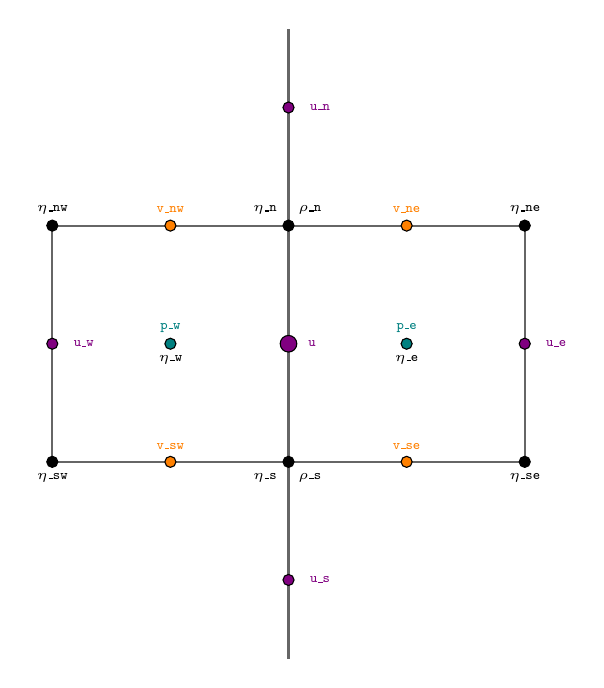
\begin{tikzpicture}
%\draw[fill=gray!23,gray!23](0,0) rectangle (8,9);
%\draw[step=0.5cm,gray,very thin] (0,0) grid (8,9); %background grid

\draw[thick,black!60] (1,3) -- (7,3) -- (7,6) -- (1,6) -- cycle ; 
\draw[thick,black!60] (4,0.5) -- (4,8.5)  ;   

%---------------------------------------------------
\node[] at (2.5,6.2) {\tiny \color{orange} \tt v\_nw};
\node[] at (2.5,3.2) {\tiny \color{orange} \tt v\_sw};
\node[] at (5.5,6.2) {\tiny \color{orange} \tt v\_ne};
\node[] at (5.5,3.2) {\tiny \color{orange} \tt v\_se};
\draw[black,fill=orange] (2.5,6)   circle (2pt);
\draw[black,fill=orange] (2.5,3)   circle (2pt);
\draw[black,fill=orange] (5.5,6)   circle (2pt);
\draw[black,fill=orange] (5.5,3)   circle (2pt);

%--------------------------------------------------
\draw[black,fill=violet] (4,1.5)   circle (2pt);
\draw[black,fill=violet] (4,4.5)   circle (3pt);
\draw[black,fill=violet] (4,7.5)   circle (2pt);
\draw[black,fill=violet] (1,4.5)   circle (2pt);
\draw[black,fill=violet] (7,4.5)   circle (2pt);
\node[] at (4.4,1.5) {\tiny \color{violet} \tt u\_s};
\node[] at (4.3,4.5) {\tiny \color{violet} \tt u};
\node[] at (4.4,7.5) {\tiny \color{violet} \tt u\_n};
\node[] at (1.4,4.5) {\tiny \color{violet} \tt u\_w};
\node[] at (7.4,4.5) {\tiny \color{violet} \tt u\_e};

\draw[black,fill=black] (1,3)   circle (2pt); 
\draw[black,fill=black] (4,3)   circle (2pt); 
\draw[black,fill=black] (7,3)   circle (2pt); 
\draw[black,fill=black] (1,6)   circle (2pt); 
\draw[black,fill=black] (4,6)   circle (2pt); 
\draw[black,fill=black] (7,6)   circle (2pt); 

%------------------------------------------------
\draw[black,fill=teal] (2.5,4.5)   circle (2pt);
\draw[black,fill=teal] (5.5,4.5)   circle (2pt);
\node[] at (2.5,4.7) {\tiny \color{teal} \tt p\_w};
\node[] at (5.5,4.7) {\tiny \color{teal} \tt p\_e};

\node[] at (4.27,2.8) {\tiny \tt $\rho$\_s};
\node[] at (4.27,6.2) {\tiny \tt $\rho$\_n};
\node[] at (2.5,4.3) {\tiny \tt $\eta$\_w};
\node[] at (5.5,4.3) {\tiny \tt $\eta$\_e};
\node[] at (3.7,2.8) {\tiny \tt $\eta$\_s};
\node[] at (3.7,6.2) {\tiny \tt $\eta$\_n};
\node[] at (7,6.2) {\tiny \tt $\eta$\_{ne}};
\node[] at (1,6.2) {\tiny \tt $\eta$\_{nw}};
\node[] at (7,2.8) {\tiny \tt $\eta$\_{se}};
\node[] at (1,2.8) {\tiny \tt $\eta$\_{sw}};
\end{tikzpicture}
\end{center}



\columnbreak

\begin{flushright} {\tiny {\color{gray} (tikz\_staggered2D\_v.tex)}} \end{flushright}
%~~~~~~~~~~~~~~~~~~~~~~~~~~~~~~~~~~~~~~~~~~~~~~~~~~~~~~~~~~~~~~~~~~~~~~~~~~~~~~~~~~~~~~~~~~~~~~~~~~



\begin{center}
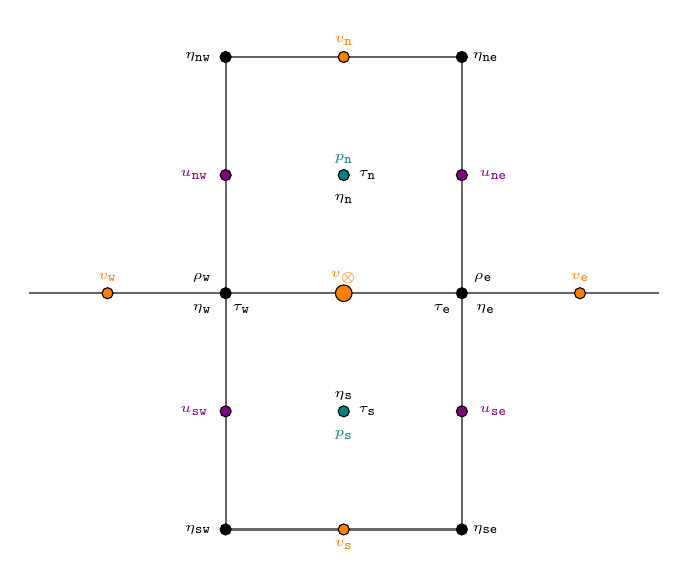
\begin{tikzpicture}
%\draw[fill=gray!23,gray!23](0,0) rectangle (9,8);
%\draw[step=0.5cm,gray,very thin] (0,0) grid (9,8); %background grid
\draw[thick,black!60] (3,1) -- (3,7) -- (6,7) -- (6,1) -- cycle ; 
\draw[thick,black!60] (0.5,4) -- (8.5,4)  ;   
%---------------------------------------------------
\node[] at (4.5,.8) {\tiny \color{orange} $v_{\tt s}$};
\node[] at (4.5,7.2) {\tiny \color{orange} $v_{\tt n}$};
\node[] at (4.5,4.2) {\tiny \color{orange} $v_\otimes$};
\node[] at (1.5,4.2) {\tiny \color{orange} $v_{\tt w}$};
\node[] at (7.5,4.2) {\tiny \color{orange} $v_{\tt e}$};
\draw[black,fill=orange] (4.5,1)   circle (2pt);
\draw[black,fill=orange] (4.5,4)   circle (3pt);
\draw[black,fill=orange] (4.5,7)   circle (2pt);
\draw[black,fill=orange] (1.5,4)   circle (2pt);
\draw[black,fill=orange] (7.5,4)   circle (2pt);
%--------------------------------------------------
\draw[black,fill=violet] (3,2.5)   circle (2pt);
\draw[black,fill=violet] (6,2.5)   circle (2pt);
\draw[black,fill=violet] (3,5.5)   circle (2pt);
\draw[black,fill=violet] (6,5.5)   circle (2pt);
\node[] at (2.6,2.5) {\tiny \color{violet} $u_{\tt sw}$};
\node[] at (6.4,2.5) {\tiny \color{violet} $u_{\tt se}$};
\node[] at (2.6,5.5) {\tiny \color{violet} $u_{\tt nw}$};
\node[] at (6.4,5.5) {\tiny \color{violet} $u_{\tt ne}$};
%-----------------------------------------------
\draw[black,fill=black] (3,1)   circle (2pt); 
\draw[black,fill=black] (3,4)   circle (2pt); 
\draw[black,fill=black] (3,7)   circle (2pt); 
\draw[black,fill=black] (6,1)   circle (2pt); 
\draw[black,fill=black] (6,4)   circle (2pt); 
\draw[black,fill=black] (6,7)   circle (2pt); 
%------------------------------------------------
\draw[black,fill=teal] (4.5,2.5)   circle (2pt);
\draw[black,fill=teal] (4.5,5.5)   circle (2pt);
\node[] at (4.5,2.2) {\tiny \color{teal} $p_{\tt s}$};
\node[] at (4.5,5.7) {\tiny \color{teal} $p_{\tt n}$};
%-----------------------------------------
\node[] at (6.27,4.2) {\tiny $\rho_{\tt e}$};
\node[] at (2.7,4.2) {\tiny $\rho_{\tt w}$};
\node[] at (4.5,5.2) {\tiny $\eta_{\tt n}$};
\node[] at (4.5,2.7) {\tiny $\eta_{\tt s}$};
\node[] at (6.3,1) {\tiny $\eta_{\tt se}$};
\node[] at (2.65,1) {\tiny $\eta_{\tt sw}$};
\node[] at (6.3,7) {\tiny $\eta_{\tt ne}$};
\node[] at (2.65,7) {\tiny $\eta_{\tt nw}$};
\node[] at (6.3,3.8) {\tiny $\eta_{\tt e}$};
\node[] at (2.7,3.8) {\tiny $\eta_{\tt w}$};

\node[] at (3.2,3.8) {\tiny $\tau_{\tt w}$};
\node[] at (5.75,3.8) {\tiny $\tau_{\tt e}$};
\node[] at (4.8,5.5) {\tiny $\tau_{\tt n}$};
\node[] at (4.8,2.5) {\tiny $\tau_{\tt s}$};


\end{tikzpicture}
\end{center}



\end{multicols}

On the left side, we see that it would be trivial to compute $\partial u/\partial x$
and $\partial u/\partial y$ on node ${\color{violet} u_\otimes}$:
\begin{eqnarray}
\frac{\partial u}{\partial x} |_{\color{violet}\otimes}
&\simeq&  \frac{ {\color{violet} u_e}-{\color{violet} u_w}  }{2h_x} \nn\\
\frac{\partial u}{\partial y} |_{\color{violet}\otimes}
&\simeq&  \frac{ {\color{violet} u_n}-{\color{violet} u_s}  }{2h_y} \nn
\end{eqnarray}
Likewise, on the right we could easily compute
\begin{eqnarray}
\frac{\partial v}{\partial x} |_{\color{orange}\otimes}
&\simeq&  \frac{ {\color{orange} v_e}-{\color{orange} v_w}  }{2h_x} \nn\\
\frac{\partial v}{\partial y} |_{\color{orange}\otimes}
&\simeq&  \frac{ {\color{orange} v_n}-{\color{orange} v_s}  }{2h_y} \nn
\end{eqnarray}
Conversely, on the left side it would be difficult to 
compute any $v$ derivative because no horizontal or vertical 
line passing by the $u$ node in the middle intersects with a 
$v$ node, and vice versa on the right side. 

It then looks like our best option to compute $\dot{\varepsilon}_{xy}$
terms is actually on the background (black) nodes since 
on the left we would have
\[
\dot{\varepsilon}_{xy}|_{\tt n} 
= 
\frac12 \left(  
\frac{\partial u}{\partial y}|_{\tt n}
+
\frac{\partial v}{\partial x}|_{\tt n}
\right)
\simeq 
\frac12 
\left( 
\frac{{\color{violet}u_{\tt n}} -{\color{violet}u_\otimes}}{h_y} + 
\frac{{\color{orange}v_{\tt ne}}-{\color{orange}u_{\tt nw}}}{h_x} 
\right)
\]
This is indeed what we find in Gerya's book at p.~137:
\begin{center}
\includegraphics[width=6cm]{images/fdm/gerya_H}\\
{\captionfont Taken from Gerya (2019).}
\end{center}
However, we need to be careful with those nodes on the boundary, and
even more careful with those at the corners of the domain. 

Let us look again at our prototype mesh:

\begin{flushright} {\tiny {\color{gray} (tikz\_staggered2D\_4x3.tex)}} \end{flushright}
%~~~~~~~~~~~~~~~~~~~~~~~~~~~~~~~~~~~~~~~~~~~~~~~~~~~~~~~~~~~~~~~~~~~~~~~~~~~~~~~~~~~~~~~~~~~~~~~~~~


\begin{center}
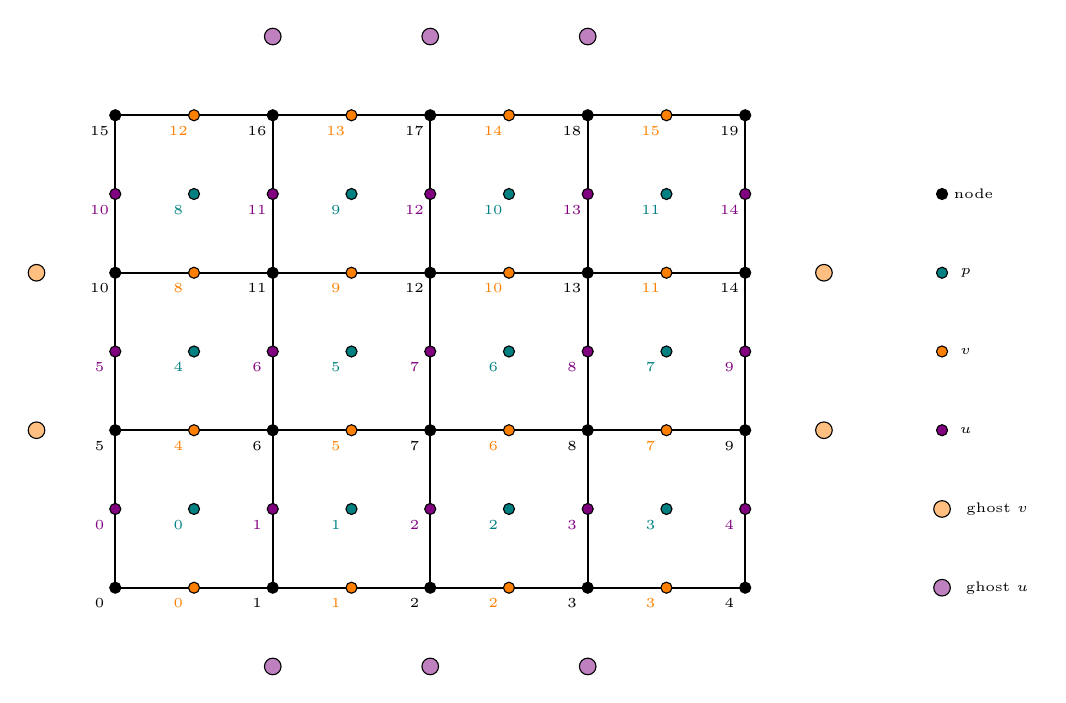
\begin{tikzpicture}
%\draw[fill=gray!23,gray!23](0,0) rectangle (12,10);
%\draw[step=0.5cm,gray,very thin] (0,0) grid (12,10); %background grid

\draw[thick] (0,0) -- (8,0) -- (8,6) -- (0,6) -- cycle ; %1-4
\draw[thick] (0,2) -- (8,2)  ; 
\draw[thick] (0,4) -- (8,4)  ; 
\draw[thick] (2,0) -- (2,6)  ; 
\draw[thick] (4,0) -- (4,6)  ; 
\draw[thick] (6,0) -- (6,6)  ; 

%pressure nodes
\draw[black,fill=teal] (1,1)   circle (2pt); 
\draw[black,fill=teal] (3,1)   circle (2pt); 
\draw[black,fill=teal] (5,1)   circle (2pt); 
\draw[black,fill=teal] (7,1)   circle (2pt); 

\draw[black,fill=teal] (1,3)   circle (2pt); 
\draw[black,fill=teal] (3,3)   circle (2pt); 
\draw[black,fill=teal] (5,3)   circle (2pt); 
\draw[black,fill=teal] (7,3)   circle (2pt); 

\draw[black,fill=teal] (1,5)   circle (2pt); 
\draw[black,fill=teal] (3,5)   circle (2pt); 
\draw[black,fill=teal] (5,5)   circle (2pt); 
\draw[black,fill=teal] (7,5)   circle (2pt); 

\node[] at (0.8,0.8) {\tiny \color{teal} 0};
\node[] at (2.8,0.8) {\tiny \color{teal} 1};
\node[] at (4.8,0.8) {\tiny \color{teal} 2};
\node[] at (6.8,0.8) {\tiny \color{teal} 3};

\node[] at (0.8,2.8) {\tiny \color{teal} 4};
\node[] at (2.8,2.8) {\tiny \color{teal} 5};
\node[] at (4.8,2.8) {\tiny \color{teal} 6};
\node[] at (6.8,2.8) {\tiny \color{teal} 7};

\node[] at (0.8,4.8) {\tiny \color{teal} 8};
\node[] at (2.8,4.8) {\tiny \color{teal} 9};
\node[] at (4.8,4.8) {\tiny \color{teal} 10};
\node[] at (6.8,4.8) {\tiny \color{teal} 11};

% u nodes
\draw[black,fill=violet] (0,1)   circle (2pt); 
\draw[black,fill=violet] (2,1)   circle (2pt); 
\draw[black,fill=violet] (4,1)   circle (2pt); 
\draw[black,fill=violet] (6,1)   circle (2pt); 
\draw[black,fill=violet] (8,1)   circle (2pt); 

\draw[black,fill=violet] (0,3)   circle (2pt); 
\draw[black,fill=violet] (2,3)   circle (2pt); 
\draw[black,fill=violet] (4,3)   circle (2pt); 
\draw[black,fill=violet] (6,3)   circle (2pt);
\draw[black,fill=violet] (8,3)   circle (2pt);

\draw[black,fill=violet] (0,5)   circle (2pt); 
\draw[black,fill=violet] (2,5)   circle (2pt); 
\draw[black,fill=violet] (4,5)   circle (2pt); 
\draw[black,fill=violet] (6,5)   circle (2pt);
\draw[black,fill=violet] (8,5)   circle (2pt);

\node[] at (-0.2,0.8) {\tiny \color{violet} 0};
\node[] at (1.8,0.8)  {\tiny \color{violet} 1};
\node[] at (3.8,0.8)  {\tiny \color{violet} 2};
\node[] at (5.8,0.8)  {\tiny \color{violet} 3};
\node[] at (7.8,0.8)  {\tiny \color{violet} 4};

\node[] at (-0.2,2.8) {\tiny \color{violet} 5};
\node[] at (1.8,2.8)  {\tiny \color{violet} 6};
\node[] at (3.8,2.8)  {\tiny \color{violet} 7};
\node[] at (5.8,2.8)  {\tiny \color{violet} 8};
\node[] at (7.8,2.8)  {\tiny \color{violet} 9};

\node[] at (-0.2,4.8){\tiny \color{violet} 10};
\node[] at (1.8,4.8) {\tiny \color{violet} 11};
\node[] at (3.8,4.8) {\tiny \color{violet} 12};
\node[] at (5.8,4.8) {\tiny \color{violet} 13};
\node[] at (7.8,4.8) {\tiny \color{violet} 14};

% v nodes
\draw[black,fill=orange] (1,0)   circle (2pt); 
\draw[black,fill=orange] (3,0)   circle (2pt); 
\draw[black,fill=orange] (5,0)   circle (2pt); 
\draw[black,fill=orange] (7,0)   circle (2pt); 

\draw[black,fill=orange] (1,2)   circle (2pt); 
\draw[black,fill=orange] (3,2)   circle (2pt); 
\draw[black,fill=orange] (5,2)   circle (2pt); 
\draw[black,fill=orange] (7,2)   circle (2pt); 

\draw[black,fill=orange] (1,4)   circle (2pt); 
\draw[black,fill=orange] (3,4)   circle (2pt); 
\draw[black,fill=orange] (5,4)   circle (2pt); 
\draw[black,fill=orange] (7,4)   circle (2pt); 

\draw[black,fill=orange] (1,6)   circle (2pt); 
\draw[black,fill=orange] (3,6)   circle (2pt); 
\draw[black,fill=orange] (5,6)   circle (2pt); 
\draw[black,fill=orange] (7,6)   circle (2pt); 

\node[] at (0.8,-0.2) {\tiny \color{orange} 0};
\node[] at (2.8,-0.2) {\tiny \color{orange} 1};
\node[] at (4.8,-0.2) {\tiny \color{orange} 2};
\node[] at (6.8,-0.2) {\tiny \color{orange} 3};

\node[] at (0.8,1.8) {\tiny \color{orange} 4};
\node[] at (2.8,1.8) {\tiny \color{orange} 5};
\node[] at (4.8,1.8) {\tiny \color{orange} 6};
\node[] at (6.8,1.8) {\tiny \color{orange} 7};

\node[] at (0.8,3.8) {\tiny \color{orange} 8};
\node[] at (2.8,3.8) {\tiny \color{orange} 9};
\node[] at (4.8,3.8) {\tiny \color{orange} 10};
\node[] at (6.8,3.8) {\tiny \color{orange} 11};

\node[] at (0.8,5.8) {\tiny \color{orange} 12};
\node[] at (2.8,5.8) {\tiny \color{orange} 13};
\node[] at (4.8,5.8) {\tiny \color{orange} 14};
\node[] at (6.8,5.8) {\tiny \color{orange} 15};

%------------------------------------------------

\draw[black,fill=black] (0,0)   circle (2pt); 
\draw[black,fill=black] (2,0)   circle (2pt); 
\draw[black,fill=black] (4,0)   circle (2pt); 
\draw[black,fill=black] (6,0)   circle (2pt); 
\draw[black,fill=black] (8,0)   circle (2pt); 

\draw[black,fill=black] (0,2)   circle (2pt); 
\draw[black,fill=black] (2,2)   circle (2pt); 
\draw[black,fill=black] (4,2)   circle (2pt); 
\draw[black,fill=black] (6,2)   circle (2pt); 
\draw[black,fill=black] (8,2)   circle (2pt); 

\draw[black,fill=black] (0,4)   circle (2pt); 
\draw[black,fill=black] (2,4)   circle (2pt); 
\draw[black,fill=black] (4,4)   circle (2pt); 
\draw[black,fill=black] (6,4)   circle (2pt); 
\draw[black,fill=black] (8,4)   circle (2pt); 

\draw[black,fill=black] (0,6)   circle (2pt); 
\draw[black,fill=black] (2,6)   circle (2pt); 
\draw[black,fill=black] (4,6)   circle (2pt); 
\draw[black,fill=black] (6,6)   circle (2pt); 
\draw[black,fill=black] (8,6)   circle (2pt); 


\node[] at (-0.2,-0.2){\tiny 0};
\node[] at (1.8,-0.2) {\tiny 1};
\node[] at (3.8,-0.2) {\tiny 2};
\node[] at (5.8,-0.2) {\tiny 3};
\node[] at (7.8,-0.2) {\tiny 4};

\node[] at (-0.2,1.8){\tiny 5};
\node[] at (1.8,1.8) {\tiny 6};
\node[] at (3.8,1.8) {\tiny 7};
\node[] at (5.8,1.8) {\tiny 8};
\node[] at (7.8,1.8) {\tiny 9};

\node[] at (-0.2,3.8){\tiny 10};
\node[] at (1.8,3.8) {\tiny 11};
\node[] at (3.8,3.8) {\tiny 12};
\node[] at (5.8,3.8) {\tiny 13};
\node[] at (7.8,3.8) {\tiny 14};

\node[] at (-0.2,5.8){\tiny 15};
\node[] at (1.8,5.8) {\tiny 16};
\node[] at (3.8,5.8) {\tiny 17};
\node[] at (5.8,5.8) {\tiny 18};
\node[] at (7.8,5.8) {\tiny 19};

%-------------------------------------------------

\draw[black,fill=black]  (10.5,5)   circle (2pt); \node[] at (10.9,5) {\tiny node};
\draw[black,fill=teal]   (10.5,4)   circle (2pt); \node[] at (10.8,4) {\tiny $p$};
\draw[black,fill=orange] (10.5,3)   circle (2pt); \node[] at (10.8,3) {\tiny $v$};
\draw[black,fill=violet] (10.5,2)   circle (2pt); \node[] at (10.8,2) {\tiny $u$};

\draw[black,fill=orange!50] (10.5,1)  circle (3pt); \node[] at (11.2,1) {\tiny ghost $v$};
\draw[black,fill=violet!50] (10.5,0)  circle (3pt); \node[] at (11.2,0) {\tiny ghost $u$};

%boundary u nodes
\draw[black,fill=violet!50] (2,-1)   circle (3pt); 
\draw[black,fill=violet!50] (4,-1)   circle (3pt); 
\draw[black,fill=violet!50] (6,-1)   circle (3pt); 
\draw[black,fill=violet!50] (2,7)   circle (3pt); 
\draw[black,fill=violet!50] (4,7)   circle (3pt); 
\draw[black,fill=violet!50] (6,7)   circle (3pt); 

%boundary u nodes
\draw[black,fill=orange!50] (-1,2)   circle (3pt); 
\draw[black,fill=orange!50] (-1,4)   circle (3pt); 
\draw[black,fill=orange!50] (9,2)   circle (3pt); 
\draw[black,fill=orange!50] (9,4)   circle (3pt); 





\end{tikzpicture}
\end{center}



Let us consider node 10. It is `missing' a left neighbour, which is 
the ghost node of ${\color{orange} v_{8}}$. 
Still operating under the assumption that boundary conditions are either 
free slip or no slip, the velocity assigned to this ghost is $\delta_{bc} {\color{orange} v_{8}}$,
so that 
\[
\dot{\varepsilon}_{xy}|_{\tt 10} 
= 
\frac12 \left(  
\frac{\partial u}{\partial y}|_{\tt 10}
+
\frac{\partial v}{\partial x}|_{\tt 10}
\right)
\simeq 
\frac12 
\left( 
\frac{{\color{violet}u_{\tt 10}} -{\color{violet}u_5}}{h_y} + 
\frac{{\color{orange}v_{\tt 8}}- \delta_{bc}{\color{orange}u_{\tt 8}}}{h_x} 
\right)
\]
Likewise, for node 3, we see that the ghost node of ${\color{violet} v_3}$
will be needed:
\[
\dot{\varepsilon}_{xy}|_{\tt 3} 
= 
\frac12 \left(  
\frac{\partial u}{\partial y}|_{\tt 3}
+
\frac{\partial v}{\partial x}|_{\tt 3}
\right)
\simeq 
\frac12 
\left( 
\frac{{\color{violet}u_{\tt 3}} -\delta_{bc} {\color{violet}u_{\tt 3}}}{h_y} + 
\frac{{\color{orange}v_{\tt 3}}- {\color{orange}u_{\tt 2}}}{h_x} 
\right)
\]
As for the corners, let us consider node 15. 
We would need the ghost node of ${\color{orange} v_{\tt 12}}$, but since 
it would be on the top boundary its $v$ value would also be zero. 
Likewise we would need the ghost node of ${\color{violet} u_{\tt 10}}$
but it would be on the left boundary so its $u$ value would be zero.
In the end we find that $\dot{\varepsilon}_{xy}=0$ in all four corners.






%------------------------------------------------------------------------
\subsection{Embedding of Particle-In-Cell}

how to interpolate fields onto particles?

section 8.4, 8.5 of book

%------------------------------------------------------------------------
\subsection{Measure errors}

TODO

%------------------------------------------------------------------------
\subsection{Non-equidistant nodes \label{ss:fdm_stokes_hvar}}

TODO

























\newpage
\begin{landscape}
{\tiny
\[
\left(
\begin{array}{c|c|c|c|c|c|c|c|c|c|c|c|c|c|c|c|c|c|c|c|c|c|c|c|c|c|c|c|c|c|c|c|c|c|c|c|c|c|c|c|c|c|c}
1 & 2 & 3 & 4 & 5 & 6 & 7 & 8 & 9 &
10 & 11 &12 &13 &14 &15& 16& 17& 18& 19 &
20 &21 &22 &23 & 24 & 25 & 26 & 27 & 28 & 29 &
30 &21 &22 &23 & 24 & 25 & 26 & 27 & 28 & 29 &
40 & 41 & 42 & 43 \\
. & . & . & . & . & . & . & . & . & . & . & . & . & . & . & . & . & . & . & . & . & . & . & . & . & 
. & . & . & . & . & . & . & . & . & . & . & . & . & . & . & . & . & . \\
. & . & . & . & . & . & . & . & . & . & . & . & . & . & . & . & . & . & . & . & . & . & . & . & . & 
. & . & . & . & . & . & . & . & . & . & . & . & . & . & . & . & . & . \\
. & . & . & . & . & . & . & . & . & . & . & . & . & . & . & . & . & . & . & . & . & . & . & . & . & 
. & . & . & . & . & . & . & . & . & . & . & . & . & . & . & . & . & . \\
. & . & . & . & . & . & . & . & . & . & . & . & . & . & . & . & . & . & . & . & . & . & . & . & . & 
. & . & . & . & . & . & . & . & . & . & . & . & . & . & . & . & . & . \\
. & . & . & . & . & . & . & . & . & . & . & . & . & . & . & . & . & . & . & . & . & . & . & . & . & 
. & . & . & . & . & . & . & . & . & . & . & . & . & . & . & . & . & . \\
. & . & . & . & . & . & . & . & . & . & . & . & . & . & . & . & . & . & . & . & . & . & . & . & . & 
. & . & . & . & . & . & . & . & . & . & . & . & . & . & . & . & . & . \\
. & . & . & . & . & . & . & . & . & . & . & . & . & . & . & . & . & . & . & . & . & . & . & . & . & 
. & . & . & . & . & . & . & . & . & . & . & . & . & . & . & . & . & . \\
. & . & . & . & . & . & . & . & . & . & . & . & . & . & . & . & . & . & . & . & . & . & . & . & . & 
. & . & . & . & . & . & . & . & . & . & . & . & . & . & . & . & . & . \\
. & . & . & . & . & . & . & . & . & . & . & . & . & . & . & . & . & . & . & . & . & . & . & . & . & 
. & . & . & . & . & . & . & . & . & . & . & . & . & . & . & . & . & . \\
. & . & . & . & . & . & . & . & . & . & . & . & . & . & . & . & . & . & . & . & . & . & . & . & . & 
. & . & . & . & . & . & . & . & . & . & . & . & . & . & . & . & . & . \\
\hline
. & . & . & . & . & . & . & . & . & . & . & . & . & . & . & . & . & . & . & . & . & . & . & . & . & 
. & . & . & . & . & . & . & . & . & . & . & . & . & . & . & . & . & . \\
. & . & . & . & . & . & . & . & . & . & . & . & . & . & . & . & . & . & . & . & . & . & . & . & . & 
. & . & . & . & . & . & . & . & . & . & . & . & . & . & . & . & . & . \\
. & . & . & . & . & . & . & . & . & . & . & . & . & . & . & . & . & . & . & . & . & . & . & . & . & 
. & . & . & . & . & . & . & . & . & . & . & . & . & . & . & . & . & . \\
. & . & . & . & . & . & . & . & . & . & . & . & . & . & . & . & . & . & . & . & . & . & . & . & . & 
. & . & . & . & . & . & . & . & . & . & . & . & . & . & . & . & . & . \\
. & . & . & . & . & . & . & . & . & . & . & . & . & . & . & . & . & . & . & . & . & . & . & . & . & 
. & . & . & . & . & . & . & . & . & . & . & . & . & . & . & . & . & . \\
. & . & . & . & . & . & . & . & . & . & . & . & . & . & . & . & . & . & . & . & . & . & . & . & . & 
. & . & . & . & . & . & . & . & . & . & . & . & . & . & . & . & . & . \\
. & . & . & . & . & . & . & . & . & . & . & . & . & . & . & . & . & . & . & . & . & . & . & . & . & 
. & . & . & . & . & . & . & . & . & . & . & . & . & . & . & . & . & . \\
. & . & . & . & . & . & . & . & . & . & . & . & . & . & . & . & . & . & . & . & . & . & . & . & . & 
. & . & . & . & . & . & . & . & . & . & . & . & . & . & . & . & . & . \\
. & . & . & . & . & . & . & . & . & . & . & . & . & . & . & . & . & . & . & . & . & . & . & . & . & 
. & . & . & . & . & . & . & . & . & . & . & . & . & . & . & . & . & . \\
. & . & . & . & . & . & . & . & . & . & . & . & . & . & . & . & . & . & . & . & . & . & . & . & . & 
. & . & . & . & . & . & . & . & . & . & . & . & . & . & . & . & . & . \\
\hline
. & . & . & . & . & . & . & . & . & . & . & . & . & . & . & . & . & . & . & . & . & . & . & . & . & 
. & . & . & . & . & . & . & . & . & . & . & . & . & . & . & . & . & . \\
. & . & . & . & . & . & . & . & . & . & . & . & . & . & . & . & . & . & . & . & . & . & . & . & . & 
. & . & . & . & . & . & . & . & . & . & . & . & . & . & . & . & . & . \\
. & . & . & . & . & . & . & . & . & . & . & . & . & . & . & . & . & . & . & . & . & . & . & . & . & 
. & . & . & . & . & . & . & . & . & . & . & . & . & . & . & . & . & . \\
. & . & . & . & . & . & . & . & . & . & . & . & . & . & . & . & . & . & . & . & . & . & . & . & . & 
. & . & . & . & . & . & . & . & . & . & . & . & . & . & . & . & . & . \\
. & . & . & . & . & . & . & . & . & . & . & . & . & . & . & . & . & . & . & . & . & . & . & . & . & 
. & . & . & . & . & . & . & . & . & . & . & . & . & . & . & . & . & . \\
. & . & . & . & . & . & . & . & . & . & . & . & . & . & . & . & . & . & . & . & . & . & . & . & . & 
. & . & . & . & . & . & . & . & . & . & . & . & . & . & . & . & . & . \\
. & . & . & . & . & . & . & . & . & . & . & . & . & . & . & . & . & . & . & . & . & . & . & . & . & 
. & . & . & . & . & . & . & . & . & . & . & . & . & . & . & . & . & . \\
. & . & . & . & . & . & . & . & . & . & . & . & . & . & . & . & . & . & . & . & . & . & . & . & . & 
. & . & . & . & . & . & . & . & . & . & . & . & . & . & . & . & . & . \\
. & . & . & . & . & . & . & . & . & . & . & . & . & . & . & . & . & . & . & . & . & . & . & . & . & 
. & . & . & . & . & . & . & . & . & . & . & . & . & . & . & . & . & . \\
. & . & . & . & . & . & . & . & . & . & . & . & . & . & . & . & . & . & . & . & . & . & . & . & . & 
. & . & . & . & . & . & . & . & . & . & . & . & . & . & . & . & . & . \\
\hline
. & . & . & . & . & . & . & . & . & . & . & . & . & . & . & . & . & . & . & . & . & . & . & . & . & 
. & . & . & . & . & . & . & . & . & . & . & . & . & . & . & . & . & . \\
. & . & . & . & . & . & . & . & . & . & . & . & . & . & . & . & . & . & . & . & . & . & . & . & . & 
. & . & . & . & . & . & . & . & . & . & . & . & . & . & . & . & . & . \\
. & . & . & . & . & . & . & . & . & . & . & . & . & . & . & . & . & . & . & . & . & . & . & . & . & 
. & . & . & . & . & . & . & . & . & . & . & . & . & . & . & . & . & . \\
. & . & . & . & . & . & . & . & . & . & . & . & . & . & . & . & . & . & . & . & . & . & . & . & . & 
. & . & . & . & . & . & . & . & . & . & . & . & . & . & . & . & . & . \\
. & . & . & . & . & . & . & . & . & . & . & . & . & . & . & . & . & . & . & . & . & . & . & . & . & 
. & . & . & . & . & . & . & . & . & . & . & . & . & . & . & . & . & . \\
. & . & . & . & . & . & . & . & . & . & . & . & . & . & . & . & . & . & . & . & . & . & . & . & . & 
. & . & . & . & . & . & . & . & . & . & . & . & . & . & . & . & . & . \\
. & . & . & . & . & . & . & . & . & . & . & . & . & . & . & . & . & . & . & . & . & . & . & . & . & 
. & . & . & . & . & . & . & . & . & . & . & . & . & . & . & . & . & . \\
. & . & . & . & . & . & . & . & . & . & . & . & . & . & . & . & . & . & . & . & . & . & . & . & . & 
. & . & . & . & . & . & . & . & . & . & . & . & . & . & . & . & . & . \\
. & . & . & . & . & . & . & . & . & . & . & . & . & . & . & . & . & . & . & . & . & . & . & . & . & 
. & . & . & . & . & . & . & . & . & . & . & . & . & . & . & . & . & . \\
. & . & . & . & . & . & . & . & . & . & . & . & . & . & . & . & . & . & . & . & . & . & . & . & . & 
. & . & . & . & . & . & . & . & . & . & . & . & . & . & . & . & . & . \\
\hline
. & . & . & . & . & . & . & . & . & . & . & . & . & . & . & . & . & . & . & . & . & . & . & . & . & 
. & . & . & . & . & . & . & . & . & . & . & . & . & . & . & . & . & . \\
. & . & . & . & . & . & . & . & . & . & . & . & . & . & . & . & . & . & . & . & . & . & . & . & . & 
. & . & . & . & . & . & . & . & . & . & . & . & . & . & . & . & . & . \\
. & . & . & . & . & . & . & . & . & . & . & . & . & . & . & . & . & . & . & . & . & . & . & . & . & 
. & . & . & . & . & . & . & . & . & . & . & . & . & . & . & . & . & . 
\end{array}
\right)
%\cdot
%\vec{X}=
%\left(
%\begin{array}{c}
%0 \\ . \\ . \\ 0 \\ 0 \\ . \\ . \\ 0 \\
%X \\
%0 \\ 0 \\ 0 \\ 0\\ 0 \\ 0
%\end{array}
%\right)
\]
}
\end{landscape}


\newpage
\section{Solving the wave equation} \label{ss:fdm_wave_eq} 
\begin{flushright} {\tiny {\color{gray} \tt fdm\_wave\_eq.tex}} \end{flushright}
%~~~~~~~~~~~~~~~~~~~~~~~~~~~~~~~~~~~~~~~~~~~~~~~~~~~~~~~~~~~~~~~~~~~~~~~~~~~~~~~~~~~~~~~~~~~~~~~~~~

We start with the one-dimensional wave equation:
\[
u_{tt}=c^2 u_{xx}  \qquad x\in[0,L], \quad t\in[0,T]
\]
which is supplemented by the initial conditions
\begin{eqnarray}
u(x,0) &=& f(x) \qquad  \forall x\in[0,L] \nn\\
u_t(x,0) &=& g(x) \qquad  \forall x\in[0,L] 
\end{eqnarray}
and the boundary conditions
\begin{eqnarray}
u(0,t) &=& 0 \qquad  \forall t \in [0,T] \nn\\
u_t(L,t) &=& 0 \qquad  \forall t\in[0,T] \label{eq:fdm_wave_bc}
\end{eqnarray}


We then proceed to discretise the space domain with $nnx$ equidistant nodes (forming $ncellx=nnx-1$ cells)
at locations $x_i$, $i=1,...nnx$ and the time domain with $N_t$ equidistant nodes at times
$t_i$, $i=1,...N_t$.
We define $h=L/ncellx$ and $\delta\! t=T/(N_t-1)$

We are looking for the solution $u(x,t)$ at all mesh points in space in time and denote by 
$u_i^k$ the discrete solution at location $x_i$ and time $t_k$.

Following Section~\ref{XYZ} the second-order derivatives will be replaced by central differences 
stencils, i.e. for a function $f$ we would write
\[
\frac{\partial^2  f}{\partial t^2} \simeq \frac{ f^{k+1} -2f^{k} +f^{k-1}  }{\delta\! t^2}
\]

%-----------------------------------
\subsection{Simple explicit method}
\label{ss:fdmwavess}

The first idea is just to use central differences for both time and space derivatives,
while assuming that the rhs (space) term is taken at time $t_k$:
i.e.
\[
\frac{ u_i^{k+1} -2u_i^{k} +u_i^{k-1}  }{\delta\! t^2} = 
c^2
\frac{ u_{i+1}^k -2u_{i}^k +u_{i-1}^k  }{h^2} 
\]
We then define $\alpha = c\; \delta\! t / h$, so that we can write the equation above as
\begin{equation}
u_i^{k+1} -2u_i^{k} +u_i^{k-1}  = \alpha^2 (u_{i+1}^k -2u_{i}^k +u_{i-1}^k )
\label{eq:fdmwave1}
\end{equation}
or,
\begin{mdframed}[backgroundcolor=blue!5]
\begin{equation}
u_i^{k+1} = - u_i^{k-1} +2(1-\alpha^2) u_{i}^k + \alpha^2 (u_{i+1}^k +u_{i-1}^k ) 
\label{eq:wavee3}
\end{equation}
\end{mdframed}
The parameter $\alpha$ is important and is often denoted by $C$ or $C_{CFL}$ as it is the 
Courant–Friedrichs–Lewy number\footnote{\url{https://en.wikipedia.org/wiki/Courant-Friedrichs-Lewy_condition}}.

Of course, we need to be careful about the initial conditions. Indeed, looking 
at the left hand side of Eq.~\eqref{eq:fdmwave1}, we see that we have three values of $u_i$
at three consecutive different times.
In other words, in order to compute $u_i^{k+1}$ we need two previous values 
of $u_i$, i.e. $u_i^{k-1}$ and $u_{i}^k$. 

The relationship above can be written for any node inside the domain but not for those on the 
boundaries ($x=0,L$). However this is not a problem since we need not to write such an equation
as the values of $u$ at the extremities of the domain are given by the boundary conditions of 
Eq.~\eqref{eq:fdm_wave_bc}.

The initial condition on $u$ is trivial to implement. But quid of $u_t$? In this case we would 
write a centered difference as 
\[
g(x_i)=\left. \frac{\partial u}{\partial t} \right|_{i}^0 \simeq \frac{u_i^1-u_i^{-1}}{2 \delta \! t} 
\]
so that 
\[
u_i^{-1} = u_i^1 - 2 \delta \! t \; g(x_i)
\]
and then, when inserted in Eq.~\eqref{eq:wavee3}, we get for $k=0$
\begin{eqnarray}
u_i^{1} 
&=& - u_i^{-1} +2(1-\alpha^2) u_{i}^0 + \alpha^2 (u_{i+1}^0 +u_{i-1}^0)  \nn\\
&=& - (u_i^1 - 2 \delta \! t g(x_i))  +2(1-\alpha^2) u_{i}^0 + \alpha^2 (u_{i+1}^0 +u_{i-1}^0)  \nn\\
2 u_i^1 &=& 2 \delta \! t g(x_i)  +2(1-\alpha^2) u_{i}^0 + \alpha^2 (u_{i+1}^0 +u_{i-1}^0)  \nn\\
u_i^1 &=&  \delta \! t g(x_i)  + (1-\alpha^2) f(x_{i}) + \frac{\alpha^2}{2} (f(x_{i+1}) + f(x_{i-1}) \nn\\
\end{eqnarray}
We now have all discrete $u$ values for the first and second time step so we can  
apply the algorithm delineated by Eq.\eqref{eq:wavee3} to arrive at $u$ at subsequent time steps.

FIG 1 of Langtangen

{\color{red} explain that this is conditionally stable.}

%-----------------------------------
\subsection{Implicit method(s)}

We could overcome the problem of conditional stability by 
introducing an implicit scheme as follows (this time 
the space derivative terms are taken at time step $k+1$):
\[
\frac{ u_i^{k+1} -2u_i^{k} +u_i^{k-1}  }{\delta\! t^2} = 
c^2
\frac{ u_{i+1}^{k+1} -2u_{i}^{k+1} +u_{i-1}^{k+1}  }{h^2} 
\]
which leads to 
\[
u_i^{k+1} -2u_i^{k} +u_i^{k-1}  = 
\alpha ^2 ( u_{i+1}^{k+1} -2u_{i}^{k+1} +u_{i-1}^{k+1} )
\]
or,
\begin{mdframed}[backgroundcolor=blue!5]
\begin{equation}
-\alpha^2 u_{i+1}^{k+1}+
(1+2\alpha^2) u_i^{k+1} 
-\alpha^2 u_{i-1}^{k+1}
=2 u_i^k -u_i^{k-1}
\end{equation}
\end{mdframed}

Another approach (Crank-Nicolson):
\[
\frac{ u_i^{k+1} -2u_i^{k} +u_i^{k-1}  }{\delta\! t^2} = 
c^2 \frac12 \left(
\frac{ u_{i+1}^{k+1} -2u_{i}^{k+1} +u_{i-1}^{k+1}  }{h^2} 
+
\frac{ u_{i+1}^k -2u_{i}^k +u_{i-1}^k  }{h^2} 
\right)
\]


\[
u_i^{k+1} -2u_i^{k} +u_i^{k-1} 
=
\frac{\alpha^2}{2} \left(
u_{i+1}^{k+1} -2u_{i}^{k+1} +u_{i-1}^{k+1} 
+
u_{i+1}^k -2u_{i}^k +u_{i-1}^k 
\right)
\]
or,
\begin{mdframed}[backgroundcolor=blue!5]
\begin{equation}
(1+\alpha^2) u_i^{k+1} 
-\frac{\alpha^2}{2} (u_{i+1}^{k+1} +u_{i-1}^{k+1} )
=
(2-\alpha^2) u_i^{k} 
+\frac{\alpha^2}{2} (u_{i+1}^{k} +u_{i-1}^{k} )
-u_i^{k-1} 
\end{equation}
\end{mdframed}



%-------------------------------------------------------------
\subsection{Reflecting boundaries}

%-------------------------------------------------------------
\subsection{Generalisation: variable wave velocity}

%-------------------------------------------------------------
\subsection{Generalisation: damping}

%-------------------------------------------------------------
\subsection{Periodic boundary conditions}

%---------------------------------------------------------------
\subsection{(Von Neumann) Stability analysis}

%---------------------------------------------------------------
\subsection{Numerical dispersion relation}

%---------------------------------------------------------------
\subsection{Generalisation: in 2D and 3D}










 %%%%%%%%%%%%%%%%%%%%%%%%%%%%%%%%%%%%%%%%%%%%%%%%%%%%%%%%%%%%%%%%%%%%%%%%%%%%%

%%%%%%%%%%%%%%%%%%%%%%%%%%%%%%%%%%%%%%%%%%%%%%%%%%%%%%%%%%%%%%%%%%%%%%%%%%%%%%%%%%%%%%%%%%%%%%%%%%%
%\chapter{Numerical integration} %%%%%%%%%%%%%%%%%%%%%%%%%%%%%%%%%%%%%%%%%%%%%%%%%%%%%%%%%%%%%%%%%%
As we will see later, using the Finite Element method to solve problems involves computing integrals which are more often than not too complex to be computed analytically/exactly. We will then need to compute them numerically.

[wiki] In essence, 
the basic problem in numerical integration is to compute an approximate solution to a definite integral
\[
\int_a^b f(x) dx
\]
to a given degree of accuracy.
This problem has been widely studied and we know that 
if $f(x)$ is a smooth function, and the domain of integration is bounded, there are many methods for approximating the integral to the desired precision.

There are several reasons for carrying out numerical integration.
\begin{itemize}
\item The integrand $f(x)$ may be known only at certain points, such as obtained by sampling. Some embedded systems and other computer applications may need numerical integration for this reason.
\item A formula for the integrand may be known, but it may be difficult or impossible to find an antiderivative that is an elementary function. An example of such an integrand is $f(x)=exp(-x^2)$, the antiderivative of which (the error function, times a constant) cannot be written in elementary form.
\item It may be possible to find an antiderivative symbolically, but it may be easier to compute a numerical approximation than to compute the antiderivative. That may be the case if the antiderivative is given as an infinite series or product, or if its evaluation requires a special function that is not available.
\end{itemize}

%-----------------------------
\subsubsection{in 1D - theory}

The simplest method of this type is to let the interpolating function be a constant function (a polynomial of degree zero) that passes through the point $((a+b)/2, f((a+b)/2))$.

This is called the midpoint rule \index{midpoint rule} or rectangle rule. \index{rectangle rule}
\[
\int_a^b f(x)dx \simeq (b-a) f(\frac{a+b}{2})
\]

\improvement[inline]{insert here figure}

The interpolating function may be a straight line (an affine function, i.e. a polynomial of degree 1)
passing through the points $(a, f(a))$ and $(b, f(b))$.

This is called the trapezoidal rule. \index{trapezoidal rule} 
\[
\int_a^b f(x)dx \simeq (b-a) \frac{f(a)+f(b)}{2}
\]

\improvement[inline]{insert here figure}

For either one of these rules, we can make a more accurate approximation by breaking up the interval [a, b] into some number n of subintervals, computing an approximation for each subinterval, then adding up all the results. This is called a composite rule, extended rule, or iterated rule. For example, the composite trapezoidal rule can be stated as

\[
\int_a^b f(x)dx \simeq \frac{b-a}{n} \left( \frac{f(a)}{2}  
+\sum_{k=1}^{n-1} f(a+k\frac{b-a}{n})
   +\frac{f(b)}{2} \right)
\]

where the subintervals have the form $[kh,(k+1)h]$, with $h=(b-a)/n$ and $k=0,1,2,\dots,n-1$.


\begin{center}
a)\includegraphics[width=7cm]{images/quadrature/int1}
b)\includegraphics[width=7cm]{images/quadrature/int2}\\
The interval $[-2,2]$ is broken into 16 sub-intervals. The blue lines correspond to the 
approximation of the red curve by means of a) the midpoint rule,  b) the trapezoidal rule.
\end{center}

There are several algorithms for numerical integration (also commonly called 'numerical quadrature', or
simply 'quadrature') \index{quadrature}.
Interpolation with polynomials evaluated at equally spaced points in $[a,b]$
yields the Newton–Cotes formulas, of which the rectangle rule and the trapezoidal rule are examples. \index{Newton-Cotes}
If we allow the intervals between interpolation points to vary, we find another group of quadrature formulas, such as 
the Gauss(ian) quadrature formulas. \index{Gauss quadrature}
A Gaussian quadrature rule is typically more accurate than a Newton–Cotes rule, 
which requires the same number of function evaluations, if the integrand is smooth 
(i.e., if it is sufficiently differentiable).


An $n-$point Gaussian quadrature rule, named after Carl Friedrich Gauss, is a quadrature rule constructed
to yield an exact result for polynomials of degree $2n-1$ or less by a suitable choice of the points $x_i$
and weights $w_i$ for $i=1,\dots,n$.

The domain of integration for such a rule is conventionally taken as $[-1,1]$, so the rule is stated as
\[
\int_{-1}^{+1} f(x) dx = \sum_{i_q=1}^n w_{i_q} f(x_{i_q})
\]
In this formula the $x_{i_q}$ coordinate is 
the $i$-th root of the Legendre polynomial $P_n(x)$. \index{Legendre polynomial}

It is important to note that a Gaussian quadrature will only produce good results if the function $f(x)$
is well approximated by a polynomial function within the range $[-1,1]$.
As a consequence, the method is not, for example, suitable for functions with singularities.

\begin{center}
\includegraphics[width=5.cm]{images/quadrature/gq2}\\
Gauss-Legendre points and their weights.
\end{center}

As shown in the above table, it can be shown that the weight values must fulfill the following condition:
\begin{equation}
\sum_{i_q} w_{i_q}=2 \label{gq23}
\end{equation}
and it is worth noting that all quadrature point coordinates are symmetrical around the origin.

Since most quadrature formula are only valid on a specific interval, we now must address the problem 
of their use outside of such intervals. The solution turns out to be quite simple: one 
must carry out a change of variables from the interval $[a,b]$ to $[-1,1]$.

We then consider the reduced coordinate $r\in[-1,1]$ such that 
\[
r=\frac{2}{b-a}(x-a)-1 
\]
This relationship can be reversed such that when $r$ is known, its equivalent coordinate 
$x\in[a,b]$ can be computed:
\[
x=\frac{b-a}{2}(1+r)+a
\]
From this it follows that
\[
dx=\frac{b-a}{2}dr
\]
and then 
\[
\int_a^b f(x) dx  = \frac{b-a}{2} \int_{-1}^{+1} f(r) dr \simeq 
\frac{b-a}{2} \sum_{i_q=1}^n w_{i_q} f(r_{i_q})
\]

%--------------------
\subsubsection{in 1D - examples}

\paragraph{example 1}

Since we know how to carry out any required change of variables, we choose for simplicity 
$a=-1$, $b=+1$.
Let us take for example $f(x)=\pi$. Then we can compute the integral of this function 
over the interval $[a,b]$ exactly:
\[
I=\int_{-1}^{+1} f(x) dx = \pi \int_{-1}^{+1}dx  = 2 \pi
\]
We can now use a Gauss-Legendre formula to compute this same integral:
\[
I_{gq}=\int_{-1}^{+1} f(x) dx 
= \sum_{i_q=1}^{n_q} w_{i_q} f(x_{i_q}) 
= \sum_{i_q=1}^{n_q} w_{i_q} \pi
= \pi \underbrace{\sum_{i_q=1}^{n_q} w_{i_q} }_{=2}
= 2 \pi
\]
where we have used the property of the weight values of Eq.(\ref{gq23}).
Since the actual number of points was never specified, this result is valid for all 
quadrature rules.


\paragraph{example 2}

Let us now take $f(x)=m x+ p$ and repeat the same exercise:
\[
I=\int_{-1}^{+1} f(x) dx = \int_{-1}^{+1} (mx+p) dx  =  [\frac{1}{2} m x^2 + p x ]_{-1}^{+1} =2p
\]
\[
I_{gq}=\int_{-1}^{+1} f(x) dx 
\!= \sum_{i_q=1}^{n_q} w_{i_q} f(x_{i_q}) 
\!= \sum_{i_q=1}^{n_q} w_{i_q} (m x_{i_q} + p)  
\!= m \underbrace{\sum_{i_q=1}^{n_q} w_{i_q} x_{i_q}}_{=0}  + p \underbrace{\sum_{i_q=1}^{n_q} w_{i_q}}_{=2}  = 2p
\]
since the quadrature points are symmetric w.r.t. to zero on the x-axis.
Once again the quadrature is able to compute the exact value of this integral: this makes sense since 
an $n$-point rule exactly integrates a $2n-1$ order polynomial such that a 1 point quadrature exactly 
integrates a first order polynomial like the one above.



\paragraph{example 3}

Let us now take $f(x)=x^2$. We have 
\[
I=\int_{-1}^{+1} f(x) dx = \int_{-1}^{+1} x^2 dx  =  [\frac{1}{3}x^3 ]_{-1}^{+1} =  \frac{2}{3} 
\]
and 
\[
I_{gq}=\int_{-1}^{+1} f(x) dx 
\!= \sum_{i_q=1}^{n_q} w_{i_q} f(x_{i_q}) 
\!= \sum_{i_q=1}^{n_q} w_{i_q} x_{i_q}^2 
\]

\begin{itemize}
\item $n_q=1$: $x_{iq}^{(1)}=0$, $w_{i_q}=2$. $I_{gq}=0$
\item $n_q=2$: $x_{q}^{(1)}=-1/\sqrt{3}$, $x_{q}^{(2)}=1/\sqrt{3}$, $w_{q}^{(1)}=w_{q}^{(2)}=1$. $I_{gq}=\frac{2}{3}$
\item It also works $\forall n_q>2$ !
\end{itemize}

%-----------------------------
\subsubsection{in 2D/3D - theory}


Let us now turn to a two-dimensional integral of the form
\[
I=\int_{-1}^{+1} \int_{-1}^{+1} f(x,y) dx dy
\]
The equivalent Gaussian quadrature writes:
\[
I_{gq}
\simeq \sum_{i_q=1}^{n_q}\sum_{j_q}^{n_q} f(x_{i_q},y_{j_q}) w_{i_q} w_{j_q}
\]


%----------------------------------------
\subsubsection{quadrature on tetrahedra}

Quadrature rules on tetrahedra take the form:
\[
\int\int\int_{el} f(x,y,z) dxdydz = V_{el} \sum_{iq=1}^{nqel} w_{iq} f(\xi^{iq}_1,\xi^{iq}_2,\xi^{iq}_3,\xi^{iq}_4) 
\]
or, that is to say:
\[
\int\int\int_{el} f(x,y,z) dxdydz = \sum_{iq=1}^{nqel} (w_{iq}V_{el}) f(\xi^{iq}_1,\xi^{iq}_2,\xi^{iq}_3,\xi^{iq}_4) 
\]
with in our case $V_{el}=1/6$.

In the literature it can be found that a one point quadrature is characterised by 
\[
w_{iq}=1 \quad\quad\quad \xi^{iq}_1=\xi^{iq}_2=\xi^{iq}_3=\xi^{iq}_4=0.25
\]
i.e, the coordinates of the single point are given by:
\[
x_{iq}=\sum_{i=1}^4 \xi_i^{iq} x_i = \frac{1}{4} (x_1+x_2+x_3+x_4)
\]
Same for $y$ and $z$ coordinates. 

A four-point quadrature rule is characterised by $w_{iq}=0.25$ and 

\begin{tabular}{lcccc}
 & $\xi_1$ & $\xi_2$ & $\xi_3$ & $\xi_4$ \\
iq=1 & 0.585410196624969 & 0.138196601125011 & 0.138196601125011 & 0.138196601125011 \\
iq=2 & 0.138196601125011 & 0.585410196624969 & 0.138196601125011 & 0.138196601125011 \\
iq=3 & 0.138196601125011 & 0.138196601125011 & 0.585410196624969 & 0.138196601125011 \\
iq=4 & 0.138196601125011 & 0.138196601125011 & 0.138196601125011 & 0.585410196624969 
\end{tabular}
We then have:
\[
r_{iq}=\sum_{i=1}^4 \xi_i^{iq} x_i 
= (\xi_1^{iq},\xi_2^{iq},\xi_3^{iq},\xi_4^{iq})\cdot(r_1,r_2,r_3,r_4) 
= (\xi_1^{iq},\xi_2^{iq},\xi_3^{iq},\xi_4^{iq})\cdot(0,1,0,0) 
= \xi_2^{iq}
\]
\[
s_{iq}=\sum_{i=1}^4 \xi_i^{iq} y_i 
= (\xi_1^{iq},\xi_2^{iq},\xi_3^{iq},\xi_4^{iq})\cdot(s_1,s_2,s_3,s_4) 
= (\xi_1^{iq},\xi_2^{iq},\xi_3^{iq},\xi_4^{iq})\cdot(0,0,1,0) 
= \xi_3^{iq}
\]
\[
t_{iq}=\sum_{i=1}^4 \xi_i^{iq} z_i 
= (\xi_1^{iq},\xi_2^{iq},\xi_3^{iq},\xi_4^{iq})\cdot(t_1,t_2,t_3,t_4) 
= (\xi_1^{iq},\xi_2^{iq},\xi_3^{iq},\xi_4^{iq})\cdot(0,0,0,1) 
= \xi_4^{iq}
\]
Finally:

\begin{tabular}{llll}
     & $r$ & $s$ & $t$ \\
iq=1 & 0.138196601125011 & 0.138196601125011 & 0.138196601125011\\
iq=2 & 0.585410196624969 & 0.138196601125011 & 0.138196601125011\\
iq=3 & 0.138196601125011 & 0.585410196624969 & 0.138196601125011\\
iq=4 & 0.138196601125011 & 0.138196601125011 & 0.585410196624969\\
\end{tabular}





 %%%%%%%%%%%%%%%%%%%%%%%%%%%%%%%%%%%%%%%%%%%%%%%%%%%%%%%%%%%%%%%%%%%%%%%%%%%%%%

%%%%%%%%%%%%%%%%%%%%%%%%%%%%%%%%%%%%%%%%%%%%%%%%%%%%%%%%%%%%%%%%%%%%%%%%%%%%%%%%%%%%%%%%%%%%%%%%%%%
%\chapter{The building blocks of the Finite Element Method} %%%%%%%%%%%%%%%%%%%%%%%%%%%%%%%%%%%%%%%
\chapter{The building blocks of the Finite Element Method} %%%%%%%%%%%%%%%%%%%%%%%%%%%%%%%%%%%%%%%%
\begin{flushright} {\tiny {\color{gray} chapter\_fem0.tex}} \end{flushright}

\section{A bit of FE terminology}\label{sec:terminology} 
We introduce here some terminology for efficient element descriptions \cite{grsa}:
\begin{itemize}
\item For triangles/tetrahedra, the designation 
$P_m \times P_n$ \index{general}{$P_m \times P_n$}
means that each component of the velocity
is approximated by continuous piecewise \index{general}{Piecewise} complete Polynomials of degree $m$ and
pressure by continuous piecewise complete Polynomials of degree  $n$.
For example $P_2 \times P_1$ means 
\[
u \sim a_1 + a_2 x + a_3 y + a_4 xy + a_5 x^2 + a_6 y^2
\]
with similar approximations for $v$, and 
\[
p \sim b_1 + b_2x + b_3 y
\]
Both velocity and pressure are continuous across element boundaries, 
and each triangular element contains 6 velocity nodes and three pressure nodes.

\item For the same families, \index{general}{$P_m \times P_{-n}$} 
$P_m \times P_{-n}$
is as above, except that pressure is approximated via 
piecewise {\sl discontinuous} polynomials of degree $n$. For instance, $P_2 \times P_{-1}$ is the same 
as $P_2P_1$ except that pressure is now an independent linear function in each element and therefore 
discontinuous at element boundaries.

\item For quadrilaterals/hexahedra, the designation 
\index{general}{$Q_m \times Q_n$}  $Q_m \times Q_n$
means that each component of the velocity
is approximated by a continuous piecewise polynomial of degree $m$ {\sl in each direction} on the quadrilateral
and likewise for pressure, except that the polynomial is of degree $n$.
For instance,  $Q_2 \times Q_1$ \index{general}{$Q_2 \times Q_1$} means
\[
u \sim a_1 + a_2 x + a_3 y + a_4 xy + a_5 x^2 + a_6 y^2 + a_7 x^2y + a_8 xy^2 + a_9 x^2y^2
\]
and 
\[
p \sim b_1 + b_2x + b_3 y + b_4 xy
\]
\item For these same families, $Q_m \times Q_{-n}$ is as above, except that the pressure approximation 
is not continuous at element boundaries. \index{general}{$Q_m \times Q_{-n}$}

\item Again for the same families, \index{general}{$Q_m \times P_{-n}$} $Q_m \times P_{-n}$
 indicates the same velocity approximation 
with a pressure approximation that is a discontinuous complete piecewise polynomial of degree $n$
(not of degree $n$ in each direction !)

\item The designation $P_m^+$ or $Q_m^+$ means that some sort of bubble function \index{general}{Bubble Function}
was added to the polynomial approximation for the velocity. You may also find the term 'enriched element'
in the literature.

\item Finally, for $n=0$, we have piecewise-constant pressure, and we omit the minus sign for simplicity.
\end{itemize}

Another point which needs to be clarified is the use of so-called 'conforming elements' 
(or 'non-conforming elements'). \index{general}{Conforming Element} \index{general}{Non-Conforming Element}
Following again \cite{grsa}, conforming velocity elements are those for which the basis functions for a subset 
of $H^1$ for the continuous problem (the first derivatives and their squares are integrable in $\Omega$).
For instance, the rotated $Q_1 \times P_0$ element of Rannacher and Turek (see section \ref{pair}) is such that 
the velocity is discontinous across element edges, so that the derivative does not exist there. Another
typical example of non-conforming element is the Crouzeix-Raviart element \cite{crra73}.

 


 %------------------
\newpage
\section{Elements and basis functions in 1D}\label{sec:elts1D} \begin{flushright} {\tiny {\color{gray} elements1D.tex}} \end{flushright}


%------------------------------------------
\subsection{Linear basis functions ($Q_1$) \label{sec:bf1}}
\index{general}{$Q_1$}

Let $f(r)$ be a $C^1$ function on the interval $[-1:1]$ with $f(-1)=f_1$  and $f(1)=f_2$.
\begin{center}
\includegraphics[width=8cm]{images/linshapefct.png}
\end{center}
Let us assume that the function $f(r)$ is to be approximated on $[-1,1]$ by the first order polynomial 
\begin{equation}
f^h(r)=a+br \label{eqquad1}
\end{equation}
Then it must fulfil
\begin{eqnarray}
f^h(r=-1)&=&a-b =f_1 \nonumber\\
f^h(r=+1)&=&a+b =f_2 \nonumber
\end{eqnarray}
This leads to  
\begin{eqnarray}
a&=&\frac{1}{2}(f_1+f_2)  \nn\\
b&=&\frac{1}{2}(-f_1+f_2)  
\end{eqnarray}
and then replacing $a,b$ in Eq.~\eqref{eqquad1} by the above values one gets
\[
f^h(r) = \left[  \frac{1}{2}(1-r)\right] f_1 + \left[ \frac{1}{2}(1+r) \right] f_2
\]
or
\[
f^h(r)=\sum_{i=1}^2 N_i(r) f_1
\]
with
\begin{mdframed}[backgroundcolor=blue!5]
\begin{eqnarray}
N_1(r) &=& \frac{1}{2} (1-r) \nonumber\\
N_2(r) &=& \frac{1}{2} (1+r)
\end{eqnarray}
\end{mdframed}

\begin{center}
\includegraphics[width=8cm]{images/basis1D/linear.pdf}\\
{\captionfont Plot of the two linear functions $N_1(r)$ and $N_2(r)$.}
\end{center}

\newpage
%------------------------------------------
\subsection{Quadratic basis functions ($Q_2$) \label{sec:bf2}}
\index{general}{$Q_2$}

Let $f(r)$ be a $C^1$ function on the interval $[-1:1]$ with $f(-1)=f_1$, $f(0)=f_2$ and $f(1)=f_3$.
\begin{center}
\includegraphics[width=8cm]{images/quadshapefct.png}
\end{center}
Let us assume that the function $f(r)$ is to be approximated on $[-1,1]$ by the second order polynomial 
$f^h(r)$:
\begin{equation}
f(r)=a+br+cr^2 \label{eqquad}
\end{equation}
Then it must fulfil
\begin{eqnarray}
f^h(r=-1)&=&a-b+c = f_1 \nonumber\\
f^h(r=0) &=&a\quad\quad\quad\;     = f_2 \nonumber\\
f^h(r=+1)&=&a+b+c = f_3 \nonumber
\end{eqnarray}
This leads to
\begin{eqnarray}
a&=&f_2   \nn\\
b&=&\frac{1}{2}(-f_1+f_3)  \nn\\
c&=&\frac{1}{2}(f_1+f_3-2f_2) 
\end{eqnarray}
and then replacing $a,b,c$ in Eq.~\eqref{eqquad} by the above values on gets
\[
f^h(r)=\left[\frac{1}{2}r(r-1)\right] f_1 + (1-r^2) f_2 + \left[\frac{1}{2}r(r+1)\right] f_3
\]
or,
\[
\boxed{
f^h(r) = \sum_{i=1}^3 N_i(r) f_i
}
\]
with
\begin{mdframed}[backgroundcolor=blue!5]
\begin{eqnarray}
N_1(r) &=& \frac{1}{2}r(r-1) \nonumber\\
N_2(r) &=& (1-r^2) \nonumber\\ 
N_3(r) &=& \frac{1}{2}r(r+1) 
\end{eqnarray}
\end{mdframed}

\begin{center}
\includegraphics[width=8cm]{images/basis1D/quadratic.pdf}\\
{\captionfont Plot of the three quadratic functions $N_1(r)$, $N_2(r)$ and $N_3(r)$.}
\end{center}
Note that $Q_2$ basis functions can take negative values. 

We will later need the first-order derivatives of these functions:
\begin{mdframed}[backgroundcolor=blue!5]
\begin{eqnarray}
\frac{\partial N_1}{\partial r} &=& r-\frac{1}{2} \nonumber\\
\frac{\partial N_2}{\partial r} &=& -2r \nonumber\\ 
\frac{\partial N_3}{\partial r} &=& r+\frac{1}{2}
\end{eqnarray}
\end{mdframed}


%------------------------------------------
\subsection{Cubic basis functions ($Q_3$) \label{sec:bf3}}
\index{general}{$Q_3$}

We proceed as previously by assuming that the third-order 
polynomial representation of function $f(r)$ is given by
\[
f^h(r)=a+br+cr^2+dr^3
\]
with the nodes at position -1,-1/3, +1/3 and +1.
It then must fulfil all four conditions:
\begin{eqnarray}
f(-1)   &=& a-b+c-d = f_1 \nonumber\\
f(-1/3) &=& a-\frac{b}{3}+\frac{c}{9}-\frac{d}{27} = f_2 \nonumber\\
f(+1/3) &=& a-\frac{b}{3}+\frac{c}{9}-\frac{d}{27} = f_3 \nonumber\\
f(+1)   &=& a+b+c+d = f_4 \nonumber
\end{eqnarray}
Adding the first and fourth equation and the second and third, one arrives at
\[
f_1+f_4 = 2a+2c \quad\quad\quad f_2+f_3=2a+\frac{2c}{9}
\]
and finally:
\[
a=\frac{1}{16} \left( -f_1 + 9f_2 + 9f_3 - f_4  \right)
\]
\[
c=\frac{9}{16}\left(f_1-f_2-f_3+f_4\right)
\]
Combining the original 4 equations in a different way yields
\[
2b+2d=f_4-f_1 
\quad\quad\quad
\frac{2b}{3} + \frac{2d}{27} = f_3-f_2
\]
so that
\[
b=\frac{1}{16} \left( f_1 - 27f_2 + 27f_3 -f_4   \right)
\]
\[
d=\frac{9}{16} \left( -f_1 + 3f_2 - 3f_3 + f_4 \right)
\]
Finally,
\begin{eqnarray}
f^h(r) 
&=& a+b+cr^2+dr^3 \nonumber\\
&=& \frac{1}{16} (-1+  r +9r^2 - 9r^3 )f_1 \nonumber\\ 
&+& \frac{1}{16} ( 9-27r -9r^2 +27r^3 )f_2 \nonumber\\ 
&+& \frac{1}{16} ( 9+27r -9r^2 -27r^3 )f_3 \nonumber\\ 
&+& \frac{1}{16} (-1-  r +9r^2 + 9r^3 )f_4 \nonumber\\ 
&=& \sum_{i=1}^4 N_i(r) f_i \nonumber
\end{eqnarray}
where (see also for example \cite[p49]{li06})
\begin{mdframed}[backgroundcolor=blue!5]
\begin{eqnarray}
N_1&=& \frac{1}{16} (-1+  r+9r^2- 9r^3 ) \nonumber\\ 
N_2&=& \frac{1}{16} ( 9-27r-9r^2+27r^3 ) \nonumber\\ 
N_3&=& \frac{1}{16} ( 9+27r-9r^2-27r^3 ) \nonumber\\ 
N_4&=& \frac{1}{16} (-1-  r+9r^2+ 9r^3 ) \nonumber
\end{eqnarray}
\end{mdframed}

\begin{center}
\includegraphics[width=8cm]{images/basis1D/cubic.pdf}\\
{\captionfont Plot of the four cubic functions $N_1(r)$, $N_2(r)$, $N_3(r)$ and $N_4(r)$.}
\end{center}

Let us now verify that these functions can represent any polynomial function up to third order:

\begin{itemize}
\item
Let us assume $f(r)=C$, then
\[
f^h(r) = \sum N_i(r) f_i = \sum_i N_i C = C \sum_i N_i  = C
\]
so that a constant function is exactly reproduced, as expected.
This is a very important property of the $N_i$ functions: They must fulfil $\sum\limits_i N_i =1$.

\item
Let us assume $f(r)= r$, then $f_1=-1$, $f_2=-1/3$, $f_3=1/3$ and $f_4=+1$. We then have
\begin{eqnarray}
f^h(r) 
&=& \sum N_i(r) f_i  \nonumber\\
&=& - N_1(r) -\frac{1}{3}N_2(r) + \frac{1}{3}N_3(r)  + N_4(r) \nonumber\\
&=& [-(-1+  r+9r^2- 9r^3 ) \nn\\
&&- \frac{1}{3} ( 9-27r-9r^2-27r^3 ) \nn\\
&&+ \frac{1}{3} ( 9+27r-9r^2+27r^3 ) \nn\\
&&+ (-1-  r+9r^2+ 9r^3 )]/16 \nonumber\\
&=& [-r +9r + 9r -r]/16  + ... 0 ... \nonumber\\
&=& r   
\end{eqnarray}

\item The cases $f(r)=r^2$ and $f(r)=r^3$ are left as exercise.

\end{itemize}

The basis functions first-order derivatives are given by
\begin{mdframed}[backgroundcolor=blue!5]
\begin{eqnarray}
\frac{\partial N_1}{\partial r}&=& \frac{1}{16}  (  1 +18r - 27r^2 ) \nonumber\\ 
\frac{\partial N_2}{\partial r}&=& \frac{1}{16}  (-27 -18r + 81r^2 ) \nonumber\\ 
\frac{\partial N_3}{\partial r}&=& \frac{1}{16}  (+27 -18r - 81r^2 ) \nonumber\\ 
\frac{\partial N_4}{\partial r}&=& \frac{1}{16}  ( -1 +18r + 27r^2 ) \nonumber
\end{eqnarray}
\end{mdframed}

We can also verify that the derivatives are also properly approximated:

\begin{itemize}
\item
Let us assume $f(r)=C$, then
\begin{eqnarray}
\frac{\partial f^h}{\partial r} 
&=& \sum_i \frac{\partial N_i}{\partial r} f_i  \nonumber\\
&=&  C \sum_i \frac{\partial N_i}{\partial r}  \nonumber\\
&=& \frac{C}{16} [  (  1 +18r - 27r^2 ) 
+ (-27 -18r + 81r^2 )  
+  (+27 -18r - 81r^2 ) 
+ ( -1 +18r + 27r^2 ) ]  \nonumber\\
&=& 0 \nonumber
\end{eqnarray}

\item
Let us assume $f(r)= r$, then $f_1=-1$, $f_2=-1/3$, $f_3=1/3$ and $f_4=+1$. We then have
\begin{eqnarray}
\frac{\partial f^h}{\partial r} 
&=& \sum_i \frac{\partial N_i}{\partial r} f_i  \nonumber\\
&=& \frac{1}{16} [  -(  1 +18r - 27r^2 ) 
 -\frac{1}{3} (-27 -18r + 81r^2 )  
 +\frac{1}{3} (27 -18r - 81r^2 )
 + ( -1 +18r + 27r^2 ) ]  \nonumber\\
&=& \frac{1}{16} [-2 + 18 + 54r^2 - 54r^2] \nonumber\\
&=& 1 \nonumber
\end{eqnarray}

\item
Let us assume $f(r)= r^2$, then $f_1=1$, $f_2=1/9$, $f_3=1/9$ and $f_4=1$. We then have
\begin{eqnarray}
\frac{\partial f^h}{\partial r} 
&=& \sum_i \frac{\partial N_i}{\partial r} f_i  \nonumber\\
&=& \frac{1}{16} \left[  
(  1 +18r - 27r^2 ) 
+\frac19 (-27 -18r + 81r^2 )  
+\frac19  (27 -18r - 81r^2 )
+ ( -1 +18r + 27r^2 ) \right]  \nonumber\\
&=& \frac{1}{16}(32r) \nn\\
&=& 2r
\end{eqnarray}
as expected.




\end{itemize}

%---------------------------------------------------------------
\subsection{Quartic basis functions ($Q_4$) \label{sec:bf4}}
\index{general}{$Q_4$}

The 1D basis polynomial is given by
\[
f_h(r)=a+br+cr^2+dr^3+er^4
\]
with the nodes at position -1,-1/2, 0, +1/2 and +1.
The function $f^h(r)$ must then fulfil 
\begin{eqnarray}
f_h(-1)   &=& a-b+c-d+e = f_1 \nonumber\\
f_h(-1/2) &=& a-\frac{b}{2}+\frac{c}{4}-\frac{d}{8}+\frac{e}{16} = f_2 \nonumber\\
f_h(0)    &=& a = f_3 \nonumber\\
f_h(+1/2) &=& a-\frac{b}{2}+\frac{c}{4}-\frac{d}{8}+\frac{e}{16} = f_4 \nonumber\\
f_h(+1)   &=& a+b+c+d+e = f_5 \nonumber
\end{eqnarray}
or, 
\begin{equation}
\left(
\begin{array}{ccccc}
 1  &  -1  &  1 &  -1 &  1 \\ 
 1  &  -1/2  &  1/4 &  -1/8 &  1/16 \\ 
 1  &   0    &  0   &   0   & 0 \\
 1  &  1/2  &  1/4 &  1/8 &  1/16 \\ 
 1  &  1  &  1 &  1 &  1 
\end{array}
\right)
\left(
\begin{array}{c}
a \\ b \\ c \\ d \\ e
\end{array}
\right)
=
\left(
\begin{array}{c}
f_1 \\ f_2 \\ f_3 \\ f_4 \\ f_5
\end{array}
\right)
\end{equation}
The third line gives $a=f_3$ so that
\begin{equation}
\underbrace{
\left(
\begin{array}{ccccc}
-1  &  1   &  -1 &  1 \\ 
-1/2 &  1/4 & -1/8 &  1/16 \\ 
 1/2 &  1/4 &  1/8 &  1/16 \\ 
 1  &  1   &  1 &  1 
\end{array}
\right)}_{A}
\left(
\begin{array}{c}
b \\ c  \\ d \\ e
\end{array}
\right)
=
\left(
\begin{array}{c}
f_1 -f_3 \\ f_2 -f_3\\ f_4-f_3 \\ f_5 -f_3
\end{array}
\right)
\end{equation}
The inverse of the matrix $A$ is:
\[
A^{-1}=
\frac{1}{6}
\left(
\begin{array}{ccccc}
1 & -8 & 8 & -1 \\
-1 & 16 & 16 & -1 \\
-4 & 8 & -8 & 4 \\
4 & -16 & -16 & 4
\end{array}
\right)
\]
so that 
\[
\left(
\begin{array}{c}
b \\ c \\ d \\ e
\end{array}
\right)
=
\frac{1}{6}
\left(
\begin{array}{ccccc}
1 & -8 & 8 & -1 \\
-1 & 16 & 16 & -1 \\
-4 & 8 & -8 & 4 \\
4 & -16 & -16 & 4
\end{array}
\right)
\cdot
\left(
\begin{array}{c}
f_1 -f_3 \\ f_2 -f_3\\ f_4-f_3 \\ f_5 -f_3
\end{array}
\right)
\]
and then 
\begin{eqnarray}
b &=& \frac{1}{6} \left( f_1 -8f_2 +8 f_4 -f_5     \right) \\
c &=& \frac{1}{6} \left( -f_1 +16f_2 -30f_3    + 16f_4- f_5   \right) \\
d &=& \frac{1}{6} \left( -4f_1 +8f_2     -8f_4+ 4 f_5   \right) \\
e &=& \frac{1}{6} \left( 4f_1 -16f_2 +24f_3 -16f_4+ 4 f_5   \right) 
\end{eqnarray}
Finally
\begin{eqnarray}
f_h(r) 
&=& a+br+cr^2+dr^3+er^4 \nn\\
&=& f_3 + 
\frac{1}{6} \left( f_1 -8f_2 +8 f_4 -f_5     \right)  r  +
\frac{1}{6} \left( -f_1 +16f_2 -30f_3    + 16f_4- f_5   \right) r^2 + \nn\\ &&
\frac{1}{6} \left( -4f_1 +8f_2     -8f_4+ 4 f_5   \right) r^3 +
\frac{1}{6} \left( 4f_1 -16f_2 +24f_3 -16f_4+ 4 f_5   \right) r^4 \nn\\
&=& \frac{1}{6} \left(  r- r^2 -4r^3 +4r^4\right) f_1 \nn\\
&+& \frac{1}{6} \left(  -8r+16 r^2 +8r^3 -16 r^4\right) f_2 \nn\\
&+& \left( 1 -5r^2+4r^4  \right) f_3 \nn\\
&+& \frac{1}{6} \left(  8r+16 r^2 -8r^3 -16 r^4\right) f_4 \nn\\
&+& \frac{1}{6} \left(  -r- r^2 +4r^3 +4r^4\right) f_5 \nn
\end{eqnarray}
with 
\begin{mdframed}[backgroundcolor=blue!5]
\begin{eqnarray}
N_1(r)&=& \frac{1}{6} \left(  r- r^2 -4r^3 +4r^4\right) \nn\\
N_2(r)&=& \frac{1}{6} \left(  -8r+16 r^2 +8r^3 -16 r^4\right)  \nn\\
N_3(r)&=& \left( 1 -5r^2+4r^4  \right) \nn \\
N_4(r)&=& \frac{1}{6} \left(  8r+16 r^2 -8r^3 -16 r^4\right)  \nn\\
N_5(r)&=& \frac{1}{6} \left(  -r- r^2 +4r^3 +4r^4\right) 
\end{eqnarray}
\end{mdframed}

\begin{center}
\includegraphics[width=8cm]{images/basis1D/quartic.pdf}\\
{\captionfont Plot of the 5 quartic basis functions.}
\end{center}

The basis functions derivative are given by
\begin{mdframed}[backgroundcolor=blue!5]
\begin{eqnarray}
\frac{\partial N_1}{\partial r}&=& \frac{1}{6}(1-2r-12r^2+16r^3) \nn\\
\frac{\partial N_2}{\partial r}&=& \frac{1}{6}(-8+32r+24r^2-64r^3) \nn\\
\frac{\partial N_3}{\partial r}&=& -10r+16r^3 \nn\\
\frac{\partial N_4}{\partial r}&=& \frac{1}{6} (8+32r-24r^2-64r^3) \nn\\
\frac{\partial N_5}{\partial r}&=& \frac{1}{6} (-1-2r+12r^2+16r^3) 
\end{eqnarray}
\end{mdframed}


%---------------------------------------------------------------
\subsection{Fifth-order basis functions ($Q_5$) \label{sec:bf5}}
\index{general}{$Q_5$}

Following the methodology presented hereafter for $Q_6$, we arrive at 

\begin{eqnarray}
\bN_1(r) &=& -\frac{625}{768}(r+\frac35)(r+\frac15)(r-\frac15)(r-\frac35)(r-1) \nn\\
\bN_2(r) &=&  \frac{3125}{768}(r+1)(r+\frac15)(r-\frac15)(r-\frac35)(r-1) \nn\\
\bN_3(r) &=& -\frac{3125}{384}(r+1)(r+\frac35)(r-\frac15)(r-\frac35)(r-1) \nn\\
\bN_4(r) &=&  \frac{3125}{384}(r+1)(r+\frac35)(r+\frac15)(r-\frac35)(r-1) \nn\\
\bN_5(r) &=& -\frac{3125}{768}(r+1)(r+\frac35)(r+\frac15)(r-\frac15)(r-1) \nn\\
\bN_6(r) &=&  \frac{625}{768}(r+1)(r+\frac35)(r+\frac15)(r-\frac15)(r-\frac35) 
\end{eqnarray}

or, 

\begin{mdframed}[backgroundcolor=blue!5]
\begin{eqnarray}
\bN_1(r) &=& -\frac{1}{768} (625r^5-625r^4-250r^3+250r^2+9r-9) \nn\\
\bN_2(r) &=& \frac{25}{768} (125r^5-75r^4-130r^3+78r^2+5r-3) \nn\\
\bN_3(r) &=& -\frac{25}{384} (125r^5-25r^4-170r^3+34r^2+45r-9) \nn\\
\bN_4(r) &=& \frac{25}{384} (125r^5+25r^4-170r^3-34r^2+45r+9) \nn\\
\bN_5(r) &=& -\frac{25}{768} (125r^5+75r^4-130r^3-78r^2+5r+3) \nn\\
\bN_6(r) &=& \frac{1}{768} (625r^5+625r^4-250r^3-250r^2+9r+9) 
\end{eqnarray}
\end{mdframed}

with the derivatives given by

\begin{mdframed}[backgroundcolor=blue!5]
\begin{eqnarray}
\frac{\partial N_1}{\partial r}&=& -\frac{1}{768}(3125r^4-2500r^3-750r^2+500r+9 ) \nn\\ 
\frac{\partial N_2}{\partial r}&=& \frac{25}{768}(625r^4-300r^3-390r^2+156r+5  ) \nn\\ 
\frac{\partial N_3}{\partial r}&=& -\frac{25}{384}(625r^4-100r^3-510r^2+68r+45  ) \nn\\ 
\frac{\partial N_4}{\partial r}&=& \frac{25}{384}(625r^4+100r^3-510r^2-68r+45  ) \nn\\ 
\frac{\partial N_5}{\partial r}&=& -\frac{25}{768}(625r^4+300r^3-390r^2-156r+5  ) \nn\\ 
\frac{\partial N_6}{\partial r}&=& \frac{1}{768}(3125r^4+2500r^3-750r^2-500r+9 ) 
\end{eqnarray}
\end{mdframed}




\begin{center}
\includegraphics[width=11cm]{images/basis1D/Q5.pdf}\\
{\captionfont Plot of the 6 fifth-order basis functions.}
\end{center}


These functions are used in \stone~\ref{f152}.

%---------------------------------------------------------------
\subsection{Sixth-order basis functions ($Q_6$) \label{sec:bf6}}
\index{general}{$Q_6$}

The 1D basis polynomial is given by
\[
f_h(r)=a+br+cr^2+dr^3+er^4+fr^5+gr^6
\]
with the nodes at position -1,-2/3, -1/3, 0, +1/3, +2/3 and +1.
The function $f^h(r)$ must then fulfil 
%\begin{eqnarray}
%f_h(-1)   &=&  a -        b +         c -            d +e -f +g =f_1 \nn\\
%f_h(-2/3) &=&  a -\frac23 b + \frac49 c -\frac{8}{27}d +e -f +g =f_2\nn\\
%f_h(-1/3) &=&  a -\frac13 b + \frac19 c -\frac{1}{27}d +e -f +g =f_3\nn\\
%f_h(0)    &=&  a                                                = f_4 \nn\\
%f_h(+1/3) &=&  a +\frac13 b + \frac19 c +\frac{1}{27}d +e +f +g =f_5\nn\\
%f_h(+2/3) &=&  a +\frac23 b + \frac49 c +\frac{8}{27}d +e +f =g =f_6\nn\\
%f_h(+1)   &=&  a +        b +         c +            d +e +f +g =f_7 \nn
%\end{eqnarray}


\[
\left(
\begin{array}{ccccccc}
1& -1       & 1       & -1           & 1 & -1 & 1  \\
1& -\frac23 & \frac49 & -\frac{8}{27}& \frac{16}{81} & -\frac{32}{243} & \frac{64}{729}  \\
1& -\frac13 & \frac19 & -\frac{1}{27}& \frac{1}{81}  & -\frac{1}{243}  & \frac{1}{729}  \\
1& 0        & 0       & 0            &0 & 0 & 0 \\
1& \frac13  & \frac19 & \frac{1}{27} & \frac{1}{81}  & \frac{1}{243}  & \frac{1}{729}  \\
1& \frac23  & \frac49 & \frac{8}{27} & \frac{16}{81} & \frac{32}{243} & \frac{64}{729}  \\
1& 1        & 1       & 1            & 1 & 1 & 1  
\end{array}
\right)
\cdot
\left(
\begin{array}{c}
a \\ b \\ c \\ d \\ e \\ f \\ g
\end{array}
\right)
=
\left(
\begin{array}{c}
f_1 \\ f_2 \\ f_3 \\ f_4 \\ f_5 \\ f_6 \\ f_7
\end{array}
\right)
\]


The middle line yields $a=f_4$, so that we have:

\[
\left(
\begin{array}{cccccc}
 -1       & 1       & -1           & 1 & -1 & 1  \\
 -\frac23 & \frac49 & -\frac{8}{27}& \frac{16}{81} & -\frac{32}{243} & \frac{64}{729}  \\
 -\frac13 & \frac19 & -\frac{1}{27}& \frac{1}{81}  & -\frac{1}{243}  & \frac{1}{729}  \\
 \frac13  & \frac19 & \frac{1}{27} & \frac{1}{81}  & \frac{1}{243}  & \frac{1}{729}  \\
 \frac23  & \frac49 & \frac{8}{27} & \frac{16}{81} & \frac{32}{243} & \frac{64}{729}  \\
 1        & 1       & 1            & 1 & 1 & 1  
\end{array}
\right)
\cdot
\left(
\begin{array}{c}
b \\ c \\ d \\ e \\ f \\ g
\end{array}
\right)
=
\left(
\begin{array}{c}
f_1 -f_4 \\ f_2 -f_4\\ f_3 -f_4 \\ f_5 -f_4\\ f_6 -f_4\\ f_7-f_4
\end{array}
\right)
\]
Multiplying all lines by 729, we obtain:

\[
\frac{1}{729}
\left(
\begin{array}{cccccc}
 -729 & 729 & -729 & 729 & -729 & 729  \\
 -486 & 324 & -216 & 144 & -96  & 64  \\
 -243 & 81  & -27  & 9   & -3   & 1  \\
 243  & 81  & 27   & 9   & 3    & 1  \\
 486  & 324 & 216  & 144 & 96   & 64  \\
729   & 729 & 729  & 729 & 729  & 729  
\end{array}
\right)
\cdot
\left(
\begin{array}{c}
b \\ c \\ d \\ e \\ f \\ g
\end{array}
\right)
=
\left(
\begin{array}{c}
f_1 -f_4 \\ f_2 -f_4\\ f_3 -f_4 \\ f_5 -f_4\\ f_6 -f_4\\ f_7-f_4
\end{array}
\right)
\]

The inverse\footnote{\url{https://physandmathsolutions.com/Matrices/matrix_inverse/matrix_inverse_6x6.php}} of this matrix is:

\begin{verbatim}
-0.00006859 	0.00061728 	-0.00308642 	0.00308642 	-0.00061728 	0.00006859
0.00006859 	-0.00092593 	0.00925926 	0.00925926 	-0.00092593 	0.00006859
0.00077160 	-0.00617284 	0.01003086 	-0.01003086 	0.00617284 	-0.00077160
-0.00077160 	0.00925926 	-0.03009259 	-0.03009259 	0.00925926 	-0.00077160
-0.00138889 	0.00555556 	-0.00694444 	0.00694444 	-0.00555556 	0.00138889
0.00138889 	-0.00833333 	0.02083333 	0.02083333 	-0.00833333 	0.00138889
\end{verbatim}

Obviously, this is not a very practical approach anymore. One could 
solve the system by hand, making sure to keep fractions but it will be 
cumbersome. Let us turn to another approach.

The nodes inside the reference element are as follows:

\begin{verbatim}
(1) (2)  (3) (4) (5)  (6) (7)
-|---|----|---+---|----|---|-
-1 -2/3 -1/3  0  1/3  2/3  1
\end{verbatim}

Basis function $\bN_1(r)$ is a 6th order polynomial expression 
that should be 1 at node 1, and 0 at others,
i.e. at $r=-2/3,-1/3,0,1/3,2/3,1$. It must then be of the form:
\[
\bN_1(r) = \alpha(r+\frac23)(r+\frac13)(r)(r-\frac13)(r-\frac23)(r-1)
\]
When evaluated at $r=-1$, we get
\[
\bN_1(r=-1) 
= \alpha(-\frac13)(-\frac23)(-1)(-\frac43)(-\frac53)(-2)
= \alpha\frac{80}{81}
\]
Since this quantity must be 1, we have
\[
1 = \alpha \frac{80}{81}
\quad
\rightarrow
\quad
\alpha=\frac{81}{80}
\]
so that 
\begin{eqnarray}
\bN_1(r)
&=& \frac{81}{80}(r+\frac23)(r+\frac13)(r)(r-\frac13)(r-\frac23)(r-1) \nn\\
&=& \frac{81}{80} \frac{1}{81} (3r+2)(3r+1)(r)(3r-1)(3r-2)(r-1) \nn\\
&=& \frac{1}{80} (9r^2-4)(9r^2-1)(r^2-r) \nn\\
&=& \frac{1}{80} (81r^4 -45r^2 +4)(r^2-r) 
\end{eqnarray}

Moving to $\bN_2(r)$, we have
\[
\bN_2(r)= \alpha(r+1)(r+\frac13)(r)(r-\frac13)(r-\frac23)(r-1)
\]
which must be equal to 1 for $r=-2/3$:
\begin{eqnarray}
\bN_2(r=-2/3)
&=& \alpha(-\frac23+1)(-\frac23+\frac13)(-\frac23)(-\frac23-\frac13)(-\frac23-\frac23)(-\frac23-1)\nn\\
&=& \alpha (\frac13)(-\frac13)(-\frac23)(-1)(-\frac43)(-\frac53)\nn\\
&=& -\alpha \frac{40}{243}
\end{eqnarray}
so that 
\[
\bN_2(r)= -\frac{243}{40}(r+1)(r+\frac13)(r)(r-\frac13)(r-\frac23)(r-1)
\]

Moving to $\bN_3(r)$, we have
\[
\bN_3(r)= \alpha(r+1)(r+\frac23)(r)(r-\frac13)(r-\frac23)(r-1)
\]
which must be equal to 1 for $r=-1/3$:
\begin{eqnarray}
\bN_3(r=-1/3)
&=& \alpha(-\frac13+1)(-\frac13+\frac23)(-\frac13)(-\frac13-\frac13)(-\frac13-\frac23)(-\frac13-1) \nn\\
&=& \alpha(\frac23)(\frac13)(-\frac13)(-\frac23)(-1)(-\frac43) \nn\\
&=& \alpha \frac{16}{243}
\end{eqnarray}
so that 
\[
\bN_3(r)= \frac{243}{16}(r+1)(r+\frac23)(r)(r-\frac13)(r-\frac23)(r-1)
\]
Likewise, we arrive at the rest of the basis functions. In the end:

\begin{eqnarray}
\bN_1(r) &=& \frac{81}{80}(r+\frac23)(r+\frac13)(r)(r-\frac13)(r-\frac23)(r-1) \nn\\
\bN_2(r) &=& -\frac{243}{40}(r+1)(r+\frac13)(r)(r-\frac13)(r-\frac23)(r-1) \nn\\
\bN_3(r) &=& \frac{243}{16}(r+1)(r+\frac23)(r)(r-\frac13)(r-\frac23)(r-1) \nn\\
\bN_4(r) &=& -\frac{81}{4}(r+1)(r+\frac23)(r+\frac13)(r-\frac13)(r-\frac23)(r-1) \nn\\
\bN_5(r) &=& \frac{243}{16}(r+1)(r+\frac23)(r+\frac13)(r)(r-\frac23)(r-1) \nn\\
\bN_6(r) &=& -\frac{243}{40}(r+1)(r+\frac23)(r+\frac13)(r)(r-\frac13)(r-1) \nn\\
\bN_7(r) &=& \frac{81}{80}(r+1)(r+\frac23)(r+\frac13)(r)(r-\frac13)(r-\frac23)
\end{eqnarray}
or 

\begin{mdframed}[backgroundcolor=blue!5]
\begin{eqnarray}
\bN_1(r) &=& \frac{1}{80}(81r^6-81r^5-45r^4+45r^3+4r^2-4r) \nn\\
\bN_2(r) &=& -\frac{9}{40}(27r^6 -18r^5 -30r^4 +20r^3 +3r^2 -2r) \nn\\ 
\bN_3(r) &=& \frac{9}{16} (27r^6 -9r^5 -39r^4 +13r^3 +12r^2 -4r) \nn\\ 
\bN_4(r) &=& -\frac{1}{4} (81r^6 - 126r^4+49r^2 -4) \nn\\ 
\bN_5(r) &=& \frac{9}{16} (27r^6 +9r^5 -39r^4 -13r^3 +12r^2 +4r) \nn\\ 
\bN_6(r) &=& -\frac{9}{40}(27r^6 +18r^5 -30r^4 -20r^3 +3r^2 +2r) \nn\\ 
\bN_7(r) &=&  \frac{1}{80}(81r^6+81r^5-45r^4-45r^3+4r^2+4r) 
\end{eqnarray}
\end{mdframed}

\begin{center}
\includegraphics[width=11cm]{images/basis1D/Q6.pdf}\\
{\captionfont Plot of the 7 six-order basis functions.}
\end{center}

Using WolframAlpha\footnote{\url{https://www.wolframalpha.com/}}, we arrive at 

\begin{eqnarray}
\frac{d \bN_1}{dr} &=& \frac{1}{80} (486r^5 - 405r^4 - 180r^3 + 135 r^2 +8r-4) \nn\\
\frac{d \bN_2}{dr} &=& -\frac{9}{20} (81r^5 - 45r^4 -60r^3 + 30r^2 +3r -1) \nn\\ 
\frac{d \bN_3}{dr} &=& \frac{9}{16} (162r^5-45r^4 -156r^3 +39r^2 +24r -4) \nn\\ 
\frac{d \bN_4}{dr} &=& \frac{1}{2} (-243r^5+252r^3-49r) \nn\\
\frac{d \bN_5}{dr} &=& \frac{9}{16} (162r^5 +45r^4 -156r^3 -39r^2 +24r +4) \nn\\ 
\frac{d \bN_6}{dr} &=& -\frac{9}{20} (81r^5 +45r^4 -60r^3 - 30r^2 +3r +1) \nn\\ 
\frac{d \bN_7}{dr} &=& \frac{1}{80} (486r^5 + 405r^4 - 180r^3 -135r^2 +8r+4) 
\end{eqnarray}

These functions are used in \stone~\ref{f152}.





%---------------------------------------------------------------
\subsection{A generic approach to 1D basis functions \label{sec:bfgeneric}}

In order to define basis functions of order $n$ each element 
must have $n+1$ nodes.
The $i-th$ basis function for an $n-th$ order approximation
is given by:
\[
\bN_i(r) = 
\frac{
\prod_{j=0,j \ne i}^n (r-r_j)
}
{
\prod_{j=0,j \ne i}^n (r_i-r_j)
}
\]

Let us see in practice how this works and start with $n=2$ (i.e. $Q_2$ basis functions).
In the reference element we have $r_0=-1$, $r_1=0$ and $r_2=+1$, so that 
\begin{eqnarray}
\bN_0 
&=& \frac{(r-r_1)(r-r_2)}{(r_0-r_1)(r_0-r_2)} \nn\\
&=& \frac{(r-0)(r-1)}{(-1-0)(-1-1)} \nn\\
&=& \frac12 r(r-1) \nn\\
\bN_1
&=& \frac{(r-r_0)(r-r_2)}{(r_1-r_0)(r_1-r_2)} \nn\\
&=& \frac{(r+1)(r-1)}{(0+1)(0-1)} \nn\\
&=& 1-r^2 \nn\\
\bN_2 
&=& \frac{(r-r_0)(r-r_1)}{(r_2-r_0)(r_2-r_1)} \nn\\
&=& \frac{(r+1)(r-0)}{(1+1)(1-0)} \nn\\
&=& \frac12 r(r+1) 
\end{eqnarray}
These are the basis functions obtained in Section~\ref{sec:bf2}.

\todo[inline]{What about derivatives?}












\newpage

Remark:

According to Guermond\footnote{\url{https://people.tamu.edu/~guermond/M661_FALL_2015/chap2.pdf}}:
``While the choice of equidistant nodes appears somewhat natural, it is appro-
priate only when working with low-degree polynomials. The main difficulty
comes from the oscillatory nature of the Lagrange polynomials as the num-
ber of interpolation nodes grows. This phenomenon is often referred to as the
Runge phenomenon [359] (see also Meray [313]''
 %-------------
\newpage
\section{Elements and basis functions in 2D}\label{sec:shpfct2d} \begin{flushright} {\tiny {\color{gray} elements2D.tex}} \end{flushright}


Let us for a moment consider a single quadrilateral element in the $xy$-plane, 
as shown on the following figure:
\begin{center}
\includegraphics[width=5.8cm]{images/shape}
\end{center}
Let us assume that we know the values of a given field $u$ at the four vertices.
For a given point $M$ inside the element in the plane, what is the value of the 
field $u$ at this point?
It makes sense to postulate that $u_M$ will be given  by 
\[
u_M= \phi(u_1,u_2,u_3,u_4,x_M,y_M) 
\]
where $\phi$ is a function to be determined. Although $\phi$ is not unique, we can 
decide to express the value $u_M$ as a weighed sum of the values at the vertices $u_i$.
One option could be to assign all four vertices the same weight, say $1/4$ so that 
$u_M=(u_1+u_2+u_3+u_4)/4$, i.e. $u_M$ is simply given by the arithmetic mean 
of the vertices values. 
If the function $u(x,y)$ is such that it is a constant function, say $u(x,y)=C$, 
then $u_M=(u_1+u_2+u_3+u_4)/4=(C+C+C+C)/4=C$ and the result is exact.
However, for any other function $u$ the value $u_M$ will not be as accurate.
Also, this approach suffers from a major drawback as it does
not use the location of point $M$ inside the element. For instance, when 
$(x_M,y_M) \rightarrow (x_2,y_2)$ we expect $u_M \rightarrow u_2$ but $u_M$ would 
remain equal to $(u_1+u_2+u_3+u_4)/4$.

In light of this, we could now assume that the weights would depend on the position 
of $M$ in a continuous fashion:
\begin{equation}
u(x_M,y_M) = \sum_{i=1}^4 \bN_i(x_M,y_M)\;  u_i
= \bN_1(x_M,y_M) u_1 + \bN_2(x_M,y_M) u_2 + \bN_3(x_M,y_M) u_3 + \bN_4(x_M,y_M) u_4 
\end{equation}
where the $N_i$ are continuous (and also "well behaved") functions which have the property:
\[
\bN_i(x_j,y_j)=\delta_{ij}
\]
or, in other words: 
\begin{eqnarray}
\bN_3(x_1,y_1) &=& 0 \nn\\
\bN_3(x_2,y_2) &=& 0 \nn\\
\bN_3(x_3,y_3) &=& 1 \nn\\
\bN_3(x_4,y_4) &=& 0 
\end{eqnarray}
The functions $\bN_i$ are commonly called basis functions. \index{general}{basis functions}

Omitting the $M$ subscripts, the velocity components $u$ and $v$ for a point inside the element
 are given by:
\begin{eqnarray}
u^h(x,y) &=& \sum_{i=1}^4 \bN_i(x,y)\;  u_i \\
v^h(x,y) &=& \sum_{i=1}^4 \bN_i(x,y)\;  v_i \label{bf01}
\end{eqnarray}
where we have added the superscript $h$ to denote that it is an approximation of the functions 
of this element of diameter $h$. 

One can now easily compute velocity gradients (and therefore the 
strain rate tensor) since we have assumed the basis functions to be "well behaved" 
(in this case first-order differentiable):
\begin{eqnarray}
\dot{\epsilon}^h_{xx}(x,y) 
&=& \frac{\partial u^h}{\partial x} = \sum_{i=1}^4 \frac{\partial \bN_i}{\partial x}\;  u_i \\
\dot{\epsilon}^h_{yy}(x,y) 
&=& \frac{\partial v^h}{\partial y} = \sum_{i=1}^4 \frac{\partial \bN_i}{\partial y}\;  v_i \\
\dot{\epsilon}^h_{xy}(x,y) 
&=& \frac{1}{2}\left(\frac{\partial u^h}{\partial y} + \frac{\partial v^h}{\partial x} \right) 
= \frac{1}{2}\sum_{i=1}^4 \frac{\partial \bN_i}{\partial y}\;  u_i
+ \frac{1}{2}\sum_{i=1}^4 \frac{\partial \bN_i}{\partial x}\;  v_i
\end{eqnarray}
How we actually obtain the exact form of the basis functions $\bN_i$ is explained in the coming sections.



%%%%%%%%%%%%%%%%%%%%%%%%%%%%%%%%%%%%%%%%%%%%%%%%%%%%%%%%%%%%%%%%%%%%%%%%%%%%%%
\subsubsection{Bilinear basis functions in 2D ($Q_1$)} \label{ss:q12d}
\index{general}{$Q_1$}

\begin{flushright} {\tiny {\color{gray} basis\_Q1\_2D.tex}} \end{flushright}
%~~~~~~~~~~~~~~~~~~~~~~~~~~~~~~~~~~~~~~~~~~~~~~~~~~~~~~~~~~~~~~~~~~~~~~~~~~~~~~~~~~~~~~~~~~~~~~~~~~

In this section, we consider for simplicity an element which is a square defined 
by $-1<r<1$, $-1<s<1$ in the Cartesian coordinates system $(r,s)$\footnote{There is a 
reason to choose $r$ and $s$ as coordinates and not $x$ and $y$ as we will see later.}:

\input{tikz_q12d}

Note the counter-clockwise numbering\footnote{Note that in many of the python codes which 
are part of this project the numbering starts at 0.}.
This element is commonly called the reference element. How we go from the $(x,y)$ coordinate system 
to the $(r,s)$ once and vice versa will be dealt with later on.
The basis functions in the above reference element in the reduced 
coordinates system $(r,s)$ are given by:

\begin{mdframed}[backgroundcolor=blue!5]
\begin{eqnarray}
\bN_1(r,s)&=&0.25(1-r)(1-s) \nonumber\\
\bN_2(r,s)&=&0.25(1+r)(1-s) \nonumber\\
\bN_3(r,s)&=&0.25(1+r)(1+s) \nonumber\\
\bN_4(r,s)&=&0.25(1-r)(1+s) 
\end{eqnarray}
\end{mdframed}
These basis functions are the product of the linear basis functions of Section~\ref{sec:bf1}
in the $r$ direction and the $s$ direction.
The partial derivatives of these functions with respect to $r$ ans $s$ automatically follow:

\begin{mdframed}[backgroundcolor=blue!5]
\begin{align}
\frac{\partial \bN_1}{\partial r}(r,s)&= - 0.25(1-s) &
\frac{\partial \bN_1}{\partial s}(r,s)&= - 0.25(1-r) \nonumber\\
\frac{\partial \bN_2}{\partial r}(r,s)&= + 0.25(1-s) &
\frac{\partial \bN_2}{\partial s}(r,s)&= - 0.25(1+r) \nonumber\\
\frac{\partial \bN_3}{\partial r}(r,s)&= + 0.25(1+s) &
\frac{\partial \bN_3}{\partial s}(r,s)&= + 0.25(1+r) \nonumber\\
\frac{\partial \bN_4}{\partial r}(r,s)&= - 0.25(1+s) &
\frac{\partial \bN_4}{\partial s}(r,s)&= + 0.25(1-r) \nonumber
\end{align}
\end{mdframed}

Let us go back to Eq.~\eqref{bf01} and let us assume that the 
function $v(r,s)=C$ so that $v_i=C$ for $i=1,2,3,4$. 
It then follows that 
\[
v^h(r,s) = \sum_{i=1}^4 \bN_i(r,s)\;  v_i 
=C \sum_{i=1}^4 \bN_i(r,s)
=C [
\bN_1(r,s)
+\bN_2(r,s)
+\bN_3(r,s)
+\bN_4(r,s)]=C
\]
This is a very important property: if the $v$ function used to 
assign values at the vertices is constant, then 
the value of $v^h$ {\it anywhere} in the element is exactly $C$.
If we now turn to the derivatives of $v$ with respect to $r$ and $s$:
\[
\frac{\partial {v}^h}{\partial r}(r,s) 
= \sum_{i=1}^4 \frac{\partial \bN_i}{\partial r}(r,s)\;  v_i 
= C \sum_{i=1}^4 \frac{\partial \bN_i}{\partial r}(r,s) 
= C \left[ - 0.25(1-s)  + 0.25(1-s)  + 0.25(1+s)  - 0.25(1+s) \right] = 0 
\]

\[
\frac{\partial v^h}{\partial s}(r,s) 
= \sum_{i=1}^4 \frac{\partial \bN_i}{\partial s}(r,s)\;  v_i 
= C \sum_{i=1}^4 \frac{\partial \bN_i}{\partial s}(r,s) 
= C \left[ - 0.25(1-r) - 0.25(1+r) + 0.25(1+r) + 0.25(1-r) \right] = 0 
\]
We reassuringly find that the derivative of a constant field anywhere in the element is exactly zero.

If we now choose $v(r,s)=ar+bs$ with $a$ and $b$ two constant scalars, we find:
\begin{eqnarray}
v^h(r,s) 
&=& \sum_{i=1}^4 \bN_i(r,s)\;  v_i  \nn\\
&=& \sum_{i=1}^4 \bN_i(r,s) (ar_i+bs_i) \nn\\
&=& a \sum_{i=1}^4 \bN_i(r,s) r_i + b \sum_{i=1}^4 \bN_i(r,s) s_i \nn\\
&=& a \left[ 
 \frac14(1-r)(1-s)(-1)
+\frac14(1+r)(1-s)(+1)
+\frac14(1+r)(1+s)(+1)
+\frac14(1-r)(1+s)(-1) \right]  \nonumber\\
&+& b  
\left[ 
 \frac14(1-r)(1-s)(-1)
+\frac14(1+r)(1-s)(-1)
+\frac14(1+r)(1+s)(+1)
+\frac14(1-r)(1+s)(+1) \right]  \nonumber\\
&=& \frac{a}{4} \left[ 
-(1-r)(1-s)
+(1+r)(1-s)
+(1+r)(1+s)
-(1-r)(1+s) \right]  \nonumber\\
&+& \frac{b}{4}
\left[ 
-(1-r)(1-s)
-(1+r)(1-s)
+(1+r)(1+s)
+(1-r)(1+s) 
\right]  \nonumber\\
&=& ar+bs
\end{eqnarray}
This set of bilinear basis functions is therefore capable of exactly representing a bilinear field.
The derivatives are:
\begin{eqnarray}
\frac{\partial v^h}{\partial r}(r,s) 
&=& \sum_{i=1}^4 \frac{\partial \bN_i}{\partial r}(r,s)\;  v_i  \\
&=& a \sum_{i=1}^4 \frac{\partial \bN_i}{\partial r}(r,s) r_i 
+ b \sum_{i=1}^4 \frac{\partial \bN_i}{\partial r}(r,s) s_i \\
&=& a \left[
- \frac14(1-s)(-1) 
+ \frac14(1-s)(+1) 
+ \frac14(1+s)(+1) 
- \frac14(1+s)(-1) 
\right] \nonumber\\
&+&b \left[
- \frac14(1-s)(-1) 
+ \frac14(1-s)(-1) 
+ \frac14(1+s)(+1) 
- \frac14(1+s)(+1) 
\right] \nonumber\\
&=& \frac{a}{4} \left[
 (1-s)
+ (1-s)
+ (1+s)
+ (1+s)
\right] \nonumber\\
&+&\frac{b}{4} \left[
 (1-s)
- (1-s)
+ (1+s)
- (1+s)
\right] \nonumber\\
&=& a 
\end{eqnarray}
Here again, we find that the derivative of the bilinear field inside the element is exact: 
$\frac{\partial v^h}{\partial r} = \frac{\partial v}{\partial r}$.

However, following the same methodology as above, one can easily prove 
that this is no more true for polynomials of degree strictly higher than 1. 
This fact has serious consequences: if the solution to the problem at hand is 
for instance a parabola, the $Q_1$ basis functions cannot represent the solution properly, 
but only by approximating the parabola in each element by a line. As we will see 
later, $Q_2$ basis functions can remedy this problem by containing quadratic terms.

\begin{remark}
The $Q_1$ basis functions are first-order polynomials. We have seen that they can be used to compute
gradients. However they cannot be used to compute 2nd-order derivatives since their 2nd-order
derivative is identically zero.
\end{remark}




%%%%%%%%%%%%%%%%%%%%%%%%%%%%%%%%%%%%%%%%%%%%%%%%%%%%%%%%%%%%%%%%%%%%%%%%%%%%%%
\subsubsection{Biquadratic basis functions in 2D ($Q_2$)}\label{ss:q22d}
\index{general}{$Q_2$}

\begin{flushright} {\tiny {\color{gray} basis\_Q2\_2D.tex}} \end{flushright}
%~~~~~~~~~~~~~~~~~~~~~~~~~~~~~~~~~~~~~~~~~~~~~~~~~~~~~~~~~~~~~~~~~~~~~~~~~~~~~~~~~~~~~~~~~~~~~~~~~~

This element is part of the so-called Lagrange family \cite{raki00}. 
Inside an element the local numbering of the nodes is as follows\footnote{I have adopted here 
a numbering scheme starting at zero!}:

\input{tikz_q22d}

Note that this numbering is also employed in Li \cite[p56]{li06}.
The polynomial representation of the function $\phi$ over this element is then
\[
\phi^h(r,s) = a + br + cs + drs + er^2 + fs^2 + gr^2s + hrs^2 + i r^2s^2 = \sum_{i=0}^8 \bN_i(r,s) \phi_i
\]
and one can show that the basis functions are:
\begin{mdframed}[backgroundcolor=blue!5]
\begin{eqnarray}
\bN_0(r,s)&=& \frac{1}{2}r(r-1)  \frac{1}{2}s(s-1)\nonumber\\
\bN_1(r,s)&=& \frac{1}{2}r(r+1)  \frac{1}{2}s(s-1)\nonumber\\
\bN_2(r,s)&=& \frac{1}{2}r(r+1)  \frac{1}{2}s(s+1)\nonumber\\
\bN_3(r,s)&=& \frac{1}{2}r(r-1)  \frac{1}{2}s(s+1)\nonumber\\
\bN_4(r,s)&=&     (1-r^2)  \frac{1}{2}s(s-1)\nonumber\\
\bN_5(r,s)&=& \frac{1}{2}r(r+1)      (1-s^2)\nonumber\\
\bN_6(r,s)&=&     (1-r^2)  \frac{1}{2}s(s+1)\nonumber\\
\bN_7(r,s)&=& \frac{1}{2}r(r-1)      (1-s^2)\nonumber\\
\bN_8(r,s)&=&     (1-r^2)      (1-s^2)\nonumber
\end{eqnarray}
\end{mdframed}

Note that we have $\bN_i(r_j,s_j)=\delta_{ij}$ and $\bN_i(r_i,s_i)=1$. 

Their derivatives are given by:
\begin{mdframed}[backgroundcolor=blue!5]
\begin{align}
\frac{\partial \bN_0}{\partial r}&= \frac{1}{2}(2r-1)  \frac{1}{2}s(s-1) & 
\frac{\partial \bN_0}{\partial s}&= \frac{1}{2}r(r-1)  \frac{1}{2}(2s-1)\nonumber\\
\frac{\partial \bN_1}{\partial r}&= \frac{1}{2}(2r+1)  \frac{1}{2}s(s-1) &
\frac{\partial \bN_1}{\partial s}&= \frac{1}{2}r(r+1)  \frac{1}{2}(2s-1)\nonumber\\
\frac{\partial \bN_2}{\partial r}&= \frac{1}{2}(2r+1)  \frac{1}{2}s(s+1) &
\frac{\partial \bN_2}{\partial s}&= \frac{1}{2}r(r+1)  \frac{1}{2}(2s+1)\nonumber\\
\frac{\partial \bN_3}{\partial r}&= \frac{1}{2}(2r-1)  \frac{1}{2}s(s+1) &
\frac{\partial \bN_3}{\partial s}&= \frac{1}{2}r(r-1)  \frac{1}{2}(2s+1)\nonumber\\
\frac{\partial \bN_4}{\partial r}&=       (-2r)  \frac{1}{2}s(s-1) &
\frac{\partial \bN_4}{\partial s}&=     (1-r^2)  \frac{1}{2}(2s-1)\nonumber\\
\frac{\partial \bN_5}{\partial r}&= \frac{1}{2}(2r+1)     (1-s^2)&
\frac{\partial \bN_5}{\partial s}&= \frac{1}{2}r(r+1)        (-2s)\nonumber\\
\frac{\partial \bN_6}{\partial r}&=       (-2r)  \frac{1}{2}s(s+1)&
\frac{\partial \bN_6}{\partial s}&=     (1-r^2)  \frac{1}{2}(2s+1)\nonumber\\
\frac{\partial \bN_7}{\partial r}&= \frac{1}{2}(2r-1)     (1-s^2)&
\frac{\partial \bN_7}{\partial s}&= \frac{1}{2}r(r-1)        (-2s)\nonumber\\
\frac{\partial \bN_8}{\partial r}&=       (-2r)     (1-s^2)&
\frac{\partial \bN_8}{\partial s}&=     (1-r^2)        (-2s)\nonumber
\end{align}
\end{mdframed}


%%%%%%%%%%%%%%%%%%%%%%%%%%%%%%%%%%%%%%%%%%%%%%%%%%%%%%%%%%%%%%%%%%%%%%%%%%%%%%
\subsubsection{Bicubic basis functions in 2D ($Q_3$)}
\index{general}{$Q_3$}

\begin{flushright} {\tiny {\color{gray} basis\_Q3\_2D.tex}} \end{flushright}
%~~~~~~~~~~~~~~~~~~~~~~~~~~~~~~~~~~~~~~~~~~~~~~~~~~~~~~~~~~~~~~~~~~~~~~~~~~~~~~~~~~~~~~~~~~~~~~~~~~

Inside an element the local numbering of the nodes is as follows:

\input{tikz/tikz_q32d}

The 1D cubic basis functions are given by:
\begin{align}
\bN_1(r)&=(-1   +r +9r^2 - 9r^3)/16 & \bN_1(t)&=(-1   +t +9t^2 - 9t^3)/16 \nonumber\\
\bN_2(r)&=(+9 -27r -9r^2 +27r^3)/16 & \bN_2(t)&=(+9 -27t -9t^2 +27t^3)/16 \nonumber\\
\bN_3(r)&=(+9 +27r -9r^2 -27r^3)/16 & \bN_3(t)&=(+9 +27t -9t^2 -27t^3)/16 \nonumber\\
\bN_4(r)&=(-1   -r +9r^2 + 9r^3)/16 & \bN_4(t)&=(-1   -t +9t^2 + 9t^3)/16 \nonumber
\end{align}

The resulting basis functions are simply the tensor product of the above 1D ones:

\begin{mdframed}[backgroundcolor=blue!5]
\begin{eqnarray}
\bN_{01}(r,s)&=&\bN_1(r)\bN_1(s) = (-1   +r +9r^2 - 9r^3)/16 \cdot (-1  +t +9s^2 - 9s^3)/16 \nonumber\\
\bN_{02}(r,s)&=&\bN_2(r)\bN_1(s) = (+9 -27r -9r^2 +27r^3)/16 \cdot (-1  +t +9s^2 - 9s^3)/16 \nonumber\\
\bN_{03}(r,s)&=&\bN_3(r)\bN_1(s) = (+9 +27r -9r^2 -27r^3)/16 \cdot (-1  +t +9s^2 - 9s^3)/16 \nonumber\\
\bN_{04}(r,s)&=&\bN_4(r)\bN_1(s) = (-1   -r +9r^2 + 9r^3)/16 \cdot (-1  +t +9s^2 - 9s^3)/16 \nonumber\\
\bN_{05}(r,s)&=&\bN_1(r)\bN_2(s) = (-1   +r +9r^2 - 9r^3)/16 \cdot (9 -27s -9s^2 +27s^3)/16 \nonumber\\
\bN_{06}(r,s)&=&\bN_2(r)\bN_2(s) = (+9 -27r -9r^2 +27r^3)/16 \cdot (9 -27s -9s^2 +27s^3)/16 \nonumber\\
\bN_{07}(r,s)&=&\bN_3(r)\bN_2(s) = (+9 +27r -9r^2 -27r^3)/16 \cdot (9 -27s -9s^2 +27s^3)/16 \nonumber\\
\bN_{08}(r,s)&=&\bN_4(r)\bN_2(s) = (-1   -r +9r^2 + 9r^3)/16 \cdot (9 -27s -9s^2 +27s^3)/16 \nonumber\\
\bN_{09}(r,s)&=&\bN_1(r)\bN_3(s) = (-1   +r +9r^2 - 9r^3)/16 \cdot (9 +27t -9t^2 -27t^3)/16 \nn\\
\bN_{10}(r,s)&=&\bN_2(r)\bN_3(s) = (+9 -27r -9r^2 +27r^3)/16 \cdot (9 +27t -9t^2 -27t^3)/16 \nn\\
\bN_{11}(r,s)&=&\bN_3(r)\bN_3(s) = (+9 +27r -9r^2 -27r^3)/16 \cdot (9 +27t -9t^2 -27t^3)/16 \nn\\
\bN_{12}(r,s)&=&\bN_4(r)\bN_3(s) = (-1   -r +9r^2 + 9r^3)/16 \cdot (9 +27t -9t^2 -27t^3)/16 \nn\\
\bN_{13}(r,s)&=&\bN_1(r)\bN_4(s) = (-1   +r +9r^2 - 9r^3)/16 \cdot (-1   -t +9t^2 + 9t^3)/16\nn\\
\bN_{14}(r,s)&=&\bN_2(r)\bN_4(s) = (+9 -27r -9r^2 +27r^3)/16 \cdot (-1   -t +9t^2 + 9t^3)/16\nn\\
\bN_{15}(r,s)&=&\bN_3(r)\bN_4(s) = (+9 +27r -9r^2 -27r^3)/16 \cdot (-1   -t +9t^2 + 9t^3)/16\nn\\
\bN_{16}(r,s)&=&\bN_4(r)\bN_4(s) = (-1   -r +9r^2 + 9r^3)/16 \cdot (-1   -t +9t^2 + 9t^3)/16
\end{eqnarray}
\end{mdframed}

\begin{center}
\includegraphics[width=4cm]{images/basis_Q3_2D/N1}
\includegraphics[width=4cm]{images/basis_Q3_2D/N2}
\includegraphics[width=4cm]{images/basis_Q3_2D/N3}
\includegraphics[width=4cm]{images/basis_Q3_2D/N4}\\
\includegraphics[width=4cm]{images/basis_Q3_2D/N5}
\includegraphics[width=4cm]{images/basis_Q3_2D/N6}
\includegraphics[width=4cm]{images/basis_Q3_2D/N7}
\includegraphics[width=4cm]{images/basis_Q3_2D/N8}\\
\includegraphics[width=4cm]{images/basis_Q3_2D/N9}
\includegraphics[width=4cm]{images/basis_Q3_2D/N10}
\includegraphics[width=4cm]{images/basis_Q3_2D/N11}
\includegraphics[width=4cm]{images/basis_Q3_2D/N12}\\
\includegraphics[width=4cm]{images/basis_Q3_2D/N13}
\includegraphics[width=4cm]{images/basis_Q3_2D/N14}
\includegraphics[width=4cm]{images/basis_Q3_2D/N15}
\includegraphics[width=4cm]{images/basis_Q3_2D/N16}\\
{\captionfont Surface representation of the basis functions on the reference element.\\
{\color{gray} in images/basis\_Q3\_2D/ }}
\end{center}

The derivatives are trivial to obtain from the derivatives of the 1D basis functions, 
e.g.
\[
\frac{\partial \bN_{13}}{\partial r} = 
\frac{\partial \bN_{1}}{\partial r} \bN_4(s) 
\]

These basis functions are used in \stone 19.










%%%%%%%%%%%%%%%%%%%%%%%%%%%%%%%%%%%%%%%%%%%%%%%%%%%%%%%%%%%%%%%%%%%%%
\subsubsection{Eight node serendipity basis functions in 2D ($Q_2^{(8)}$)}
\label{sec:serendipity2D}
\index{general}{$Q_2^{(8)}$} 
\index{general}{Serendipity element}

\begin{flushright} {\tiny {\color{gray} basis\_Q28\_2D.tex}} \end{flushright}
%~~~~~~~~~~~~~~~~~~~~~~~~~~~~~~~~~~~~~~~~~~~~~~~~~~~~~~~~~~~~~~~~~~~~~~~~~~~~~~~~~~~~~~~~~~~~~~~~~~

The serendipity elements are those rectangular elements which have no
interior nodes (See for example Reddy \cite[p65]{reddybook2}).
Inside an element a possible local numbering of the nodes is as follows:

\input{tikz/tikz_serendipity2D}

The main difference with the $Q_2$ element resides in the fact that there is 
no node in the middle of the element.
The polynomial representation of the function $\phi$ over the element is then
\[
\phi_h(r,s) = a + br + cs + drs + er^2 + fs^2 + gr^2s + hrs^2
\]
Note that absence of the $r^2s^2$ term which was previously associated 
to the center node. We find that 
\begin{mdframed}[backgroundcolor=blue!5]
\begin{eqnarray}
\bN_0(r,s)&=& \frac{1}{4}(1-r)(1-s)(-r-s-1) \\
\bN_1(r,s)&=& \frac{1}{4}(1+r)(1-s)(r-s-1) \\
\bN_2(r,s)&=& \frac{1}{4}(1+r)(1+s)(r+s-1) \\
\bN_3(r,s)&=& \frac{1}{4}(1-r)(1+s)(-r+s-1) \\
\bN_4(r,s)&=& \frac{1}{2}(1-r^2)(1-s)  \\
\bN_5(r,s)&=& \frac{1}{2}(1+r)  (1-s^2)\\
\bN_6(r,s)&=& \frac{1}{2}(1-r^2)(1+s)  \\
\bN_7(r,s)&=& \frac{1}{2}(1-r)  (1-s^2)
\end{eqnarray}
\end{mdframed}

The basis functions at the mid side nodes are products of a 
second order polynomial parallel to side and 
a linear function perpendicular to the side
while basis functions for corner nodes are modifications of the bilinear
quadrilateral element.

\begin{center}
\includegraphics[width=4cm]{images/basis_Q28_2D/N1}
\includegraphics[width=4cm]{images/basis_Q28_2D/N2}
\includegraphics[width=4cm]{images/basis_Q28_2D/N3}
\includegraphics[width=4cm]{images/basis_Q28_2D/N4}\\
\includegraphics[width=4cm]{images/basis_Q28_2D/N5}
\includegraphics[width=4cm]{images/basis_Q28_2D/N6}
\includegraphics[width=4cm]{images/basis_Q28_2D/N7}
\includegraphics[width=4cm]{images/basis_Q28_2D/N8}\\
{\captionfont Surface representation of the basis functions on the reference element.
{\color{gray} in images/basis\_Q28\_2D/ }}
\end{center}



The first-order derivatives are given by:

\begin{mdframed}[backgroundcolor=blue!5]
\begin{eqnarray}
\frac{\partial \bN_0}{\partial r}(r,s)&=& -\frac{1}{4}(s-1)(2r+s)  \\
\frac{\partial \bN_1}{\partial r}(r,s)&=& -\frac{1}{4}(s-1)(2r-s)  \\
\frac{\partial \bN_2}{\partial r}(r,s)&=& \frac{1}{4}(s+1)(2r+s)  \\
\frac{\partial \bN_3}{\partial r}(r,s)&=& \frac{1}{4}(s+1)(2r-s)  \\
\frac{\partial \bN_4}{\partial r}(r,s)&=& r(s-1)  \\
\frac{\partial \bN_5}{\partial r}(r,s)&=& \frac{1}{2} (1-s^2)  \\
\frac{\partial \bN_6}{\partial r}(r,s)&=& -r(s+1)  \\
\frac{\partial \bN_7}{\partial r}(r,s)&=& -\frac{1}{2} (1-s^2)  
\end{eqnarray}
\end{mdframed}

\begin{mdframed}[backgroundcolor=blue!5]
\begin{eqnarray}
\frac{\partial \bN_0}{\partial s}(r,s)&=& -\frac{1}{4}(r-1)(r+2s) \\
\frac{\partial \bN_1}{\partial s}(r,s)&=& -\frac{1}{4}(r+1)(r-2s) \\
\frac{\partial \bN_2}{\partial s}(r,s)&=&  \frac{1}{4}(r+1)(r+2s) \\
\frac{\partial \bN_3}{\partial s}(r,s)&=&  \frac{1}{4}(r-1)(r-2s) \\
\frac{\partial \bN_4}{\partial s}(r,s)&=& - \frac{1}{2}(1-r^2)\\
\frac{\partial \bN_5}{\partial s}(r,s)&=&  -(r+1)s \\
\frac{\partial \bN_6}{\partial s}(r,s)&=& \frac{1}{2} (1-r^2)\\
\frac{\partial \bN_7}{\partial s}(r,s)&=&  (r-1)s
\end{eqnarray}
\end{mdframed}
These basis functions are used in \stone 52.













%%%%%%%%%%%%%%%%%%%%%%%%%%%%%%%%%%%%%%%%%%%%%%%%%%%%%%%%%%%%%%%%%%%%%
\subsubsection{Eight node serendipity basis functions in 2D ($QH8-C1$)}
\label{sec:serendipity2Db}
\index{general}{$QH8-C1$} \index{general}{Serendipity element}

This element is proposed in Zhang \& Xiang (2020) \cite{zhxi20}. Two remarks
must be made: 1) Eq.~(29) of their publication which is the definition
of the basis functions contains an error\footnote{
Answer from the author: "N5 to N8 is missing an A in the denominator and 
the calculation program does not have this problem"}. 2) The authors use a rather 
uncommon and annoying rotated numbering:
\begin{verbatim}
      y
      |
2=====5=====1             3=====6=====2
|           |             |           |   (r_0,s_0)=(-1,-1)   (r_4,s_4)=( 0,-1)
|           |             |           |   (r_1,s_1)=(+1,-1)   (r_5,s_5)=(+1, 0)
6           8--x          7     +     5   (r_2,s_2)=(+1,+1)   (r_6,s_6)=( 0,+1)
|           |             |           |   (r_3,s_3)=(-1,+1)   (r_7,s_7)=(-1, 0)
|           |             |           |    
3=====7=====4             0=====4=====1
Zhang & Xiang             our numbering
\end{verbatim}

For each element they define (their numbering):
\begin{eqnarray}
A   &=& \frac{1}{2} [ (x_1-x_3)(y_2-y_4)-(x_2-x_4)(y_1-y_3) ] \nn\\
m_x &=& (x_1-x_4)(y_2-y_3)-(x_2-x_3)(y_1-y_4) \nn\\
m_y &=& (x_3-x_4)(y_1-y_2)-(x_1-x_2)(y_3-y_4) \nn
\end{eqnarray}

Note that $A$ is the area of the element, and that in the case when 
the element is a rectangle then $m_x=m_y=0$.

\begin{eqnarray}
\bN_1(r,s)&=& n_1(r,s) +(m_x^2 - m_xm_y + m_y^2)\frac{E(r,s)}{D} \nn\\
\bN_2(r,s)&=& n_2(r,s) +(m_x^2 + m_xm_y + m_y^2)\frac{E(r,s)}{D} \nn\\
\bN_3(r,s)&=& n_3(r,s) +(m_x^2 - m_xm_y + m_y^2)\frac{E(r,s)}{D} \nn\\
\bN_4(r,s)&=& n_4(r,s) +(m_x^2 + m_xm_y + m_y^2)\frac{E(r,s)}{D} \nn\\
\bN_5(r,s)&=& n_5(r,s) -m_x(2Am_x+m_y^2)\frac{E(r,s)}{AD} \nn\\
\bN_6(r,s)&=& n_6(r,s) -m_y(2Am_y+m_x^2)\frac{E(r,s)}{AD} \nn\\
\bN_7(r,s)&=& n_7(r,s) +m_x(-2Am_x+m_y^2)\frac{E(r,s)}{AD} \nn\\
\bN_8(r,s)&=& n_8(r,s) +m_y(-2Am_y+m_x^2)\frac{E(r,s)}{AD} \nn
\end{eqnarray}
with 
\[
E(r,s)=(1-r^2)(1-s^2)
\qquad
D=4(4A^2+m_x^2+m_y^2)
\]
and where the $n_i$ functions are the basis functions of the 'regular' 
8-node element (see Section~\ref{sec:serendipity2D}).

This is implemented in \stone 52.

\todo[inline]{not finished. SHOW CONSISTENCY !! like in paper
email sent to author about mistake.  }








%%%%%%%%%%%%%%%%%%%%%%%%%%%%%%%%%%%%
\subsubsection{Biquartic basis functions in 2D ($Q_4$)}
\index{general}{$Q_4$}

Inside an element the local numbering of the nodes is as follows:

\begin{flushright} {\tiny {\color{gray} (tikz\_q42d.tex)}} \end{flushright}
%~~~~~~~~~~~~~~~~~~~~~~~~~~~~~~~~~~~~~~~~~~~~~~~~~~~~~~~~~~~~~~~~~~~~~~~~~~~~~~~~~~~~~~~~~~~~~~~~~~


\begin{center}
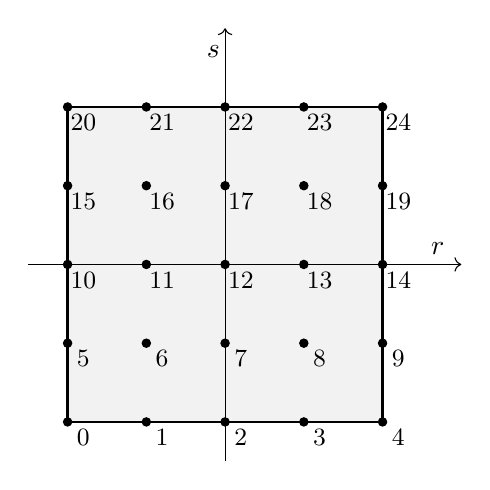
\begin{tikzpicture}
%\draw[step=0.5cm,gray,very thin] (0,0) grid (5,5); 
\draw[fill=gray!10,gray!10](1,1) rectangle (5,5);
\draw[thick] (1,1)--(5,1)--(5,5)--(1,5)--cycle;
\draw [->] (0.5,3) -- (6,3);
\draw [->] (3,0.5) -- (3,6);
\node[] at (5.7,3.2) {$r$};
\node[] at (2.85,5.7) {$s$};
\draw[black,fill=black] (1,1)   circle (1.5pt);
\draw[black,fill=black] (1,2)   circle (1.5pt);
\draw[black,fill=black] (1,3)   circle (1.5pt);
\draw[black,fill=black] (1,4)   circle (1.5pt);
\draw[black,fill=black] (1,5)   circle (1.5pt);

\draw[black,fill=black] (2,1)   circle (1.5pt);
\draw[black,fill=black] (2,2)   circle (1.5pt);
\draw[black,fill=black] (2,3)   circle (1.5pt);
\draw[black,fill=black] (2,4)   circle (1.5pt);
\draw[black,fill=black] (2,5)   circle (1.5pt);

\draw[black,fill=black] (3,1)   circle (1.5pt);
\draw[black,fill=black] (3,2)   circle (1.5pt);
\draw[black,fill=black] (3,3)   circle (1.5pt);
\draw[black,fill=black] (3,4)   circle (1.5pt);
\draw[black,fill=black] (3,5)   circle (1.5pt);

\draw[black,fill=black] (4,1)   circle (1.5pt);
\draw[black,fill=black] (4,2)   circle (1.5pt);
\draw[black,fill=black] (4,3)   circle (1.5pt);
\draw[black,fill=black] (4,4)   circle (1.5pt);
\draw[black,fill=black] (4,5)   circle (1.5pt);

\draw[black,fill=black] (5,1)   circle (1.5pt);
\draw[black,fill=black] (5,2)   circle (1.5pt);
\draw[black,fill=black] (5,3)   circle (1.5pt);
\draw[black,fill=black] (5,4)   circle (1.5pt);
\draw[black,fill=black] (5,5)   circle (1.5pt);

\node[] at (1.2,0.8) {\small $0$};
\node[] at (2.2,0.8) {\small $1$};
\node[] at (3.2,0.8) {\small $2$};
\node[] at (4.2,0.8) {\small $3$};
\node[] at (5.2,0.8) {\small $4$};

\node[] at (1.2,1.8) {\small $5$};
\node[] at (2.2,1.8) {\small $6$};
\node[] at (3.2,1.8) {\small $7$};
\node[] at (4.2,1.8) {\small $8$};
\node[] at (5.2,1.8) {\small $9$};

\node[] at (1.2,2.8) {\small $10$};
\node[] at (2.2,2.8) {\small $11$};
\node[] at (3.2,2.8) {\small $12$};
\node[] at (4.2,2.8) {\small $13$};
\node[] at (5.2,2.8) {\small $14$};

\node[] at (1.2,3.8) {\small $15$};
\node[] at (2.2,3.8) {\small $16$};
\node[] at (3.2,3.8) {\small $17$};
\node[] at (4.2,3.8) {\small $18$};
\node[] at (5.2,3.8) {\small $19$};

\node[] at (1.2,4.8) {\small $20$};
\node[] at (2.2,4.8) {\small $21$};
\node[] at (3.2,4.8) {\small $22$};
\node[] at (4.2,4.8) {\small $23$};
\node[] at (5.2,4.8) {\small $24$};

\end{tikzpicture}
\end{center}



%.....................................................................
\subsubsection{Linear basis functions for triangles in 2D ($P_1$)}\label{ss:p1}
\index{general}{$P_1$}

\begin{flushright} {\tiny {\color{gray} basis\_P1\_2D.tex}} \end{flushright}
%~~~~~~~~~~~~~~~~~~~~~~~~~~~~~~~~~~~~~~~~~~~~~~~~~~~~~~~~~~~~~~~~~~~~~~~~~~~~~~~~~~~~~~~~~~~~~~~~~~

Here we do not start from a reference element but consider instead a generic triangle:

\input{tikz/tikz_P1}

This is the simplest 2D element, which is also called linear triangular element.
Velocities (or displacements) $(u^h,v^h)$ in the element are interpolated from nodal velocities
$(u_i,v_i)$ using basis functions $\bN_i$ as follows,
\begin{small}
\[
\vec\upnu^h=
\left(
\begin{array}{c}
u^h(x,y) \\v^h(x,y)
\end{array}
\right)
=
\left(
\begin{array}{c}
\sum\limits_{i=1}^3 \bN_i(x,y) u_i \\
\sum\limits_{i=1}^3 \bN_i(x,y) v_i
\end{array}
\right)
=
\left(
\begin{array}{cccccc}
\bN_1(x,y) & 0 & \bN_2(x,y) & 0 & \bN_3(x,y) & 0\\
0 & \bN_1(x,y) & 0 & \bN_2(x,y) & 0 & \bN_3(x,y)\\
\end{array}
\right)
\cdot
\left(
\begin{array}{c}
u_1 \\ v_1 \\ u_2 \\ v_2 \\ u_3 \\ v_3
\end{array}
\right)
\]
\end{small}

For this element, we have three nodes at the vertices of the triangle, which are 
numbered around the element in the counterclockwise direction. 
Each node has two degrees of freedom (i.e. it can move in the $x$ and $y$ directions). 
The velocities $u^h$ and $v^h$ are assumed to be linear functions within the element, that is, 
\begin{eqnarray}
u^h(x,y)&=&b_1 +b_2x+b_3y \nn\\
v^h(x,y)&=&b_4 +b_5x+b_6y
\end{eqnarray}
where $b_i$ are constants to be determined and which depend on the triangle shape.
Note that the strain rate components are then given by
\begin{eqnarray}
\dot\varepsilon_{xx}(\vec\upnu)&=&b_2  \nn\\
\dot\varepsilon_{yy}(\vec\upnu)&=&b_6  \nn\\
\dot\varepsilon_{xy}(\vec\upnu)&=&(b_3+b_5)/2 \nn
\end{eqnarray}
and are constant throughout the element.

The velocities should satisfy the following six equations (when it is evaluated at a node we should 
recover the nodal velocity):
\begin{eqnarray}
u_1 &=& u^h(x_1,y_1)= b_1 + b_2x_1+b_3y_1 \nn\\
u_2 &=& u^h(x_2,y_2)= b_1 + b_2x_2+b_3y_2 \nn\\
u_3 &=& u^h(x_3,y_3)= b_1 + b_2x_3+b_3y_3 \nn\\
v_1 &=& v^h(x_1,y_1)= b_4 + b_5x_1+b_6y_1 \nn\\
v_2 &=& v^h(x_2,y_2)= b_4 + b_5x_2+b_6y_2 \nn\\
v_3 &=& v^h(x_3,y_3)= b_4 + b_5x_3+b_6y_3 \nn
\end{eqnarray}
Let us focus on the three equations with the $u$ component of the velocity.
These can be re-written:
\[
\left(
\begin{array}{c}
u_1 \\ u_2 \\ u_3  
\end{array}
\right)
=
\left(
\begin{array}{ccc}
1 & x_1 & y_1 \\
1 & x_2 & y_2 \\
1 & x_3 & y_3 \\
\end{array}
\right)
\cdot
\left(
\begin{array}{c}
b_1 \\ b_2 \\ b_3  
\end{array}
\right)
\]
In order to obtain $b_1,b_2,b_3$ we need to solve this system, or simply to compute the
inverse of the $3\times 3$ ${\bm M}$ matrix, as explained in Appendix~\ref{sec:inv3x3}.
We define $D={\rm det}({\bm M})$ and we get
\[
\left(
\begin{array}{c}
b_1 \\ b_2 \\ b_3  
\end{array}
\right)
=
\frac{1}{D}
\tilde{\bm M}
\cdot
\left(
\begin{array}{c}
u_1 \\ u_2 \\ u_3  
\end{array}
\right)
%\qquad
%{\rm and}
%\qquad
%\left(
%\begin{array}{c}
%b_4 \\ b_5 \\ b_6  
%\end{array}
%\right)
%=
%\frac{1}{D}
%\tilde{\bm M}
%\cdot
%\left(
%\begin{array}{c}
%v_1 \\ v_2 \\ v_3  
%\end{array}
%\right)
\]
The matrix $\tilde{\bm M}$ is given by:
\[
\tilde{\bm M}
%=
%\left(
%\begin{array}{ccc}
%  x_2y_3-x_3y_2  & -(y_3-y_2) &   x_3-x_2 \\
%-(x_1y_3-x_3y_1) &   y_3-y_1  & -(x_3-x_1) \\
%  x_1y_2-x_2y_1  & -(y_2-y_1) &   x_2-x_1
%\end{array}
%\right)
=
\left(
\begin{array}{ccc}
x_2y_3-x_3y_2 & x_3y_1-x_1y_3 & x_1y_2-x_2y_1 \\
y_2-y_3 & y_3-y_1  & y_1-y_2 \\
x_3-x_2 & x_1-x_3 & x_2-x_1 
\end{array}
\right)
\]
so that 
\begin{eqnarray}
b_1 &=& \frac1D [ (x_2y_3-x_3y_2)u_1 + (x_3y_1-x_1y_3)u_2 + (x_1y_2-x_2y_1)u_3 ] \nn\\
b_2 &=& \frac1D [ (y_2-y_3)u_1 + (y_3-y_1)u_2 + (y_1-y_2)u_3 ] \nn\\
b_3 &=& \frac1D [ (x_3-x_2)u_1 + (x_1-x_3)u_2 + (x_2-x_1)u_3 ]
\end{eqnarray}
We then have
\begin{eqnarray}
u^h(x,y) 
&=& b_1 + b_2 x + b_3 y \nn\\
&=&\frac1D [(x_2y_3-x_3y_2)u_1 + (x_3y_1-x_1y_3)u_2 + (x_1y_2-x_2y_1)u_3 ] \nn\\
&+&\frac1D [(y_2-y_3)u_1 + (y_3-y_1)u_2 + (y_1-y_2)u_3]x \nn\\
&+&\frac1D [(x_3-x_2)u_1 + (x_1-x_3)u_2 + (x_2-x_1)u_3]y \nn\\
&=&\frac1D [(x_2y_3-x_3y_2) + (y_2-y_3)x + (x_3-x_2)y]u_1\nn\\ 
&+&\frac1D [(x_3y_1-x_1y_3) + (y_3-y_1) x + (x_1-x_3) y]u_2 \nn\\
&+&\frac1D [(x_1y_2-x_2y_1) + (y_1-y_2) x + (x_2-x_1) y]u_3\nn\\
&=& \bN_1(x,y) u_1 + \bN_2(x,y) u_2 + \bN_3(x,y) u_3
\end{eqnarray}
with the linear basis functions are given by:
\begin{eqnarray}
\bN_1(x,y) &=& \frac{1}{D}[(x_2y_3-x_3y_2) + (y_2-y_3)x + (x_3-x_2)y] \nn\\
\bN_2(x,y) &=& \frac{1}{D}[(x_3y_1-x_1y_3) + (y_3-y_1)x + (x_1-x_3)y] \nn\\
\bN_3(x,y) &=& \frac{1}{D}[(x_1y_2-x_2y_1) + (y_1-y_2)x + (x_2-x_1)y] \nn
\end{eqnarray}
We can then easily verify that for example
\begin{eqnarray}
\bN_2(x_1,y_1)&=& \frac{1}{D}[(x_3y_1-x_1y_3) + (y_3-y_1)x_1 + (x_1-x_3)y_1] = 0 \\
\bN_2(x_2,y_2)&=& \frac{1}{D}[(x_3y_1-x_1y_3) + (y_3-y_1)x_2 + (x_1-x_3)y_2] = 1 \\
\bN_2(x_3,y_3)&=& \frac{1}{D}[(x_3y_1-x_1y_3) + (y_3-y_1)x_3 + (x_1-x_3)y_3] = 0 
\end{eqnarray}
Note that the area $A$ of the triangle is given by:
\[
A=\frac{1}{2}D = \frac{1}{2}
\left|
\begin{array}{ccc}
1 & x_1 & y_1 \\
1 & x_2 & y_2 \\
1 & x_3 & y_3 
\end{array}
\right|
\]

\noindent If we now consider the reference element in the reduced coordinates space $(r,s)$:

\input{tikz/tikz_P1ref}

The basis polynomial is then
\[
f(r,s) = a + br + cs 
\]
and the basis functions:
\begin{mdframed}[backgroundcolor=blue!5]
\begin{eqnarray}
\bN_0(r,s) &=& 1-r-s \\
\bN_1(r,s) &=& r \\
\bN_2(r,s) &=& s 
\end{eqnarray}
\end{mdframed}
Once again we can verify that $\bN_i(x_j,y_j)=\delta_{ij}$ and $\sum\limits_i \bN_i(r,s)=1$.


Coming back to the basis functions given for a generic triangle, we have
\begin{eqnarray}
\bN_1(x,y) &=& \frac{1}{D}[(x_2y_3-x_3y_2) + (y_2-y_3)x + (x_3-x_2)y] \nn\\
\bN_2(x,y) &=& \frac{1}{D}[(x_3y_1-x_1y_3) + (y_3-y_1)x + (x_1-x_3)y] \nn\\
\bN_3(x,y) &=& \frac{1}{D}[(x_1y_2-x_2y_1) + (y_1-y_2)x + (x_2-x_1)y] \nn
\end{eqnarray}
or, introducing the notations $x_{ij}=x_i-x_j$ and $y_{ij}=y_i-y_j$:
\begin{eqnarray}
\bN_1(x,y) &=& \frac{1}{D}[(x_2y_3-x_3y_2) + y_{23} x + x_{32} y] \nn\\
\bN_2(x,y) &=& \frac{1}{D}[(x_3y_1-x_1y_3) + y_{31} x + x_{13} y] \nn\\
\bN_3(x,y) &=& \frac{1}{D}[(x_1y_2-x_2y_1) + y_{12} x + x_{21} y] \nn
\end{eqnarray}
with $D=2|T|$ with $|T|$ being the area of the triangle.



The gradient matrix is then given by (see for example \cite{koko07}) 
\[
{\bm B} = 
\frac{1}{2|T|}
\begin{pmatrix}
\partial_x \bN_1 & 0 & \partial_x \bN_2 & 0 & \partial_x \bN_3 & 0 \\
0 & \partial_y \bN_1 & 0 & \partial_y \bN_2 & 0 & \partial_y \bN_3 \\
\partial_y \bN_1 & \partial_x \bN_1 &
\partial_y \bN_2 & \partial_x \bN_2 &
\partial_y \bN_3 & \partial_x \bN_3 
\end{pmatrix}
= \frac{1}{2|T|} \tilde{\bm B}
\]
with 
\[
\tilde{\bm B}=
\begin{pmatrix}
y_{23} & 0 & y_{31} & 0 & y_{12} & 0 \\
0 & x_{32} & 0 & x_{13} & 0 & x_{21} \\
x_{32} & y_{23} & x_{13} & y_{31} & x_{21} & y_{12}
\end{pmatrix}
\]

{\it What follows is written specifically for the $P_1$ element 
used in the context of elasticity and originates in \cite{koko07}.}

We can also rewrite the element displacement vector
\[
\vec{u}_e = (u_1, v_1, u_2, v_2, u_3, v_3)^T
\]
in a non-standard form
\[
\vec{u}_e = (u_1, u_2, u_3, v_1, v_2, v_3)^T
\]
Then the corresponding gradient matrix is 
\[
\tilde{\bm B}=
\begin{pmatrix}
y_{23}  & y_{31}  & y_{12} & 0 & 0 & 0 \\
0 & 0 & 0 & x_{32}  & x_{13}  & x_{21} \\
x_{32} & x_{13} & x_{21} & y_{23} &  y_{31}  & y_{12}
\end{pmatrix}
\]
We have 
\[
{\bm C} =
\begin{pmatrix}
\lambda + 2 \mu & \lambda & 0 \\
\lambda & \lambda + 2 \mu & 0 \\
0 & 0 & \mu
\end{pmatrix}
=
\begin{pmatrix}
\tilde\lambda  & \lambda & 0 \\
\lambda & \tilde\lambda  & 0 \\
0 & 0 & \mu
\end{pmatrix}
\]
Then 



\begin{landscape}
\begin{eqnarray}
&&
{\bm B}^T \cdot {\bm C} \cdot {\bm B} \nn\\
&=& \frac{1}{4|T|^2} \tilde{\bm B}^T \cdot {\bm C} \cdot \tilde{\bm B} \nn\\
&=& \frac{1}{4|T|^2} \tilde{\bm B}^T \cdot 
\begin{pmatrix}
\tilde\lambda  & \lambda & 0 \\
\lambda & \tilde\lambda  & 0 \\
0 & 0 & \mu
\end{pmatrix}
\cdot 
\begin{pmatrix}
y_{23}  & y_{31}  & y_{12} & 0 & 0 & 0 \\
0 & 0 & 0 & x_{32}  & x_{13}  & x_{21} \\
x_{32} & x_{13} & x_{21} & y_{23} &  y_{31}  & y_{12}
\end{pmatrix} \nn\\
&=& \frac{1}{4|T|^2} \tilde{\bm B}^T \cdot 
\begin{pmatrix}
\tilde\lambda y_{23} & \tilde\lambda y_{31} & \tilde\lambda y_{12} & \lambda x_{32} & \lambda x_{13} & \lambda x_{21} \\
\lambda y_{23} &  \lambda y_{31} &  \lambda y_{12} & \tilde\lambda x_{32} & \tilde\lambda x_{13} & \tilde\lambda x_{21} \\
\mu x_{32} &    \mu x_{13} & \mu x_{21} & \mu y_{23} &    \mu y_{31} & \mu y_{12}  
\end{pmatrix} \nn\\
&=&
\frac{1}{4|T|^2} 
\begin{pmatrix}
y_{23} & 0 & x_{32} \\
y_{31} & 0 & x_{13} \\
y_{12} & 0 & x_{21} \\
0 & x_{32} & y_{23} \\
0 & x_{13} & y_{31} \\
0 & x_{21} & y_{12} 
\end{pmatrix}
\cdot
\begin{pmatrix}
\tilde\lambda y_{23} & \tilde\lambda y_{31} & \tilde\lambda y_{12} & \lambda x_{32} & \lambda x_{13} & \lambda x_{21} \\
\lambda y_{23} &  \lambda y_{31} &  \lambda y_{12} & \tilde\lambda x_{32} & \tilde\lambda x_{13} & \tilde\lambda x_{21} \\
\mu x_{32} &    \mu x_{13} & \mu x_{21} & \mu y_{23} &    \mu y_{31} & \mu y_{12}  
\end{pmatrix} \nn\\
&=&
\frac{1}{4|T|^2} 
\begin{pmatrix}
\tilde\lambda y_{23}^ 2 + \mu x_{32}^2 &
\tilde\lambda y_{23}y_{31} + \mu x_{32}x_{13} &
\tilde\lambda y_{23}y_{12} + \mu x_{32}x_{21} &
\lambda y_{23}x_{32} + \mu x_{32}y_{23} &
\lambda y_{23}x_{13} + \mu x_{32}y_{31} &
\lambda y_{23}x_{21} + \mu x_{32}y_{12}  
\\
\tilde\lambda y_{31}y_{23} + \mu x_{13}x_{32} &
\tilde\lambda y_{31}^2 + \mu x_{13}^2 &
\tilde\lambda y_{31}y_{12} + \mu x_{13}x_{21} &
\lambda y_{31}x_{32} + \mu x_{13}y_{23}  &
\lambda y_{31}x_{13} + \mu x_{13}y_{31}  &
\lambda y_{31}x_{21} + \mu x_{13}y_{12}  
\\
\tilde\lambda y_{12}y_{23} + \mu x_{21}x_{32} &
\tilde\lambda y_{12}y_{31} + \mu x_{21}x_{13} &
\tilde\lambda y_{12}^2 + \mu x_{21}^2 &
\lambda y_{12}x_{32} + \mu x_{21}y_{23}  &
\lambda y_{12}x_{13} + \mu x_{21}y_{31}  &
\lambda y_{12}x_{21} + \mu x_{21}y_{12}  
\\
. & .& . &
\tilde\lambda x_{32}^2 + \mu y_{23}^2 &
\tilde\lambda x_{32}x_{13} + \mu y_{23}y_{31} &
\tilde\lambda x_{32}x_{21} + \mu y_{23}y_{12} 
\\
. & . & . & 
\tilde\lambda x_{13}x_{32} + \mu y_{31}y_{23} &
\tilde\lambda x_{13}^2 + \mu y_{31}^2 &
\tilde\lambda x_{13}x_{21} + \mu y_{31}y_{12} 
\\
. & . & . &
\tilde\lambda x_{21}x_{32} + \mu y_{12}y_{23} &
\tilde\lambda x_{21}x_{13} + \mu y_{12}y_{31} &
\tilde\lambda x_{21}^2 + \mu y_{12}^2 
\end{pmatrix} 
\nn\\
&=& \frac{1}{4|T|^2} 
\begin{pmatrix}
\K_{xx} & \K_{xy} \\
\K_{yx} & \K_{yy}
\end{pmatrix}
\end{eqnarray}
\end{landscape}

with
\begin{eqnarray}
\K_{xx} &=&  
\begin{pmatrix}
\tilde\lambda y_{23}^ 2 + \mu x_{32}^2 &
\tilde\lambda y_{23}y_{31} + \mu x_{32}x_{13} &
\tilde\lambda y_{23}y_{12} + \mu x_{32}x_{21} \\
\tilde\lambda y_{31}y_{23} + \mu x_{13}x_{32} &
\tilde\lambda y_{31}^2 + \mu x_{13}^2 &
\tilde\lambda y_{31}y_{12} + \mu x_{13}x_{21} \\
\tilde\lambda y_{12}y_{23} + \mu x_{21}x_{32} &
\tilde\lambda y_{12}y_{31} + \mu x_{21}x_{13} &
\tilde\lambda y_{12}^2 + \mu x_{21}^2 &
\end{pmatrix}
\nn\\
\K_{yy} &=&  
\begin{pmatrix}
\tilde\lambda x_{32}^2 + \mu y_{23}^2 &
\tilde\lambda x_{32}x_{13} + \mu y_{23}y_{31} &
\tilde\lambda x_{32}x_{21} + \mu y_{23}y_{12} 
\\
\tilde\lambda x_{13}x_{32} + \mu y_{31}y_{23} &
\tilde\lambda x_{13}^2 + \mu y_{31}^2 &
\tilde\lambda x_{13}x_{21} + \mu y_{31}y_{12} 
\\
\tilde\lambda x_{21}x_{32} + \mu y_{12}y_{23} &
\tilde\lambda x_{21}x_{13} + \mu y_{12}y_{31} &
\tilde\lambda x_{21}^2 + \mu y_{12}^2 
\end{pmatrix}
\nn\\
\K_{xy} = \K_{yx}^T &=&
\begin{pmatrix}
\lambda y_{23}x_{32} + \mu x_{32}y_{23} &
\lambda y_{23}x_{13} + \mu x_{32}y_{31} &
\lambda y_{23}x_{21} + \mu x_{32}y_{12}  
\\
\lambda y_{31}x_{32} + \mu x_{13}y_{23}  &
\lambda y_{31}x_{13} + \mu x_{13}y_{31}  &
\lambda y_{31}x_{21} + \mu x_{13}y_{12}  
\\
\lambda y_{12}x_{32} + \mu x_{21}y_{23}  &
\lambda y_{12}x_{13} + \mu x_{21}y_{31}  &
\lambda y_{12}x_{21} + \mu x_{21}y_{12}  
\end{pmatrix}
\end{eqnarray}

If we now introduce the vectors
\[
\vec{x} = 
\begin{pmatrix}
x_{32} \\ x_{13} \\ x_{21} 
\end{pmatrix}
\qquad \text{and}
\qquad
\vec{y}=
\begin{pmatrix}
y_{23} \\ y_{31} \\ y_{12}
\end{pmatrix}
\]
then 
\begin{eqnarray}
\K_{xx} &=&  (\lambda+2\mu) \vec{y}\vec{y}^T + \mu \vec{x}\vec{x}^T \nn\\
\K_{yy} &=&  (\lambda+2\mu) \vec{x}\vec{x}^T + \mu \vec{y}\vec{y}^T \nn\\
\K_{xy} &=& \lambda \vec{y}\vec{x}^T  + \mu \vec{x} \vec{y}^T \nn
\end{eqnarray}

In the end 
\begin{eqnarray}
\K 
&=& \int_T {\bm B}^T \cdot {\bm C} \cdot {\bm B} dV \nn\\
&=& \int_T \frac{1}{4|T|^2} \tilde{\bm B}^T \cdot {\bm C} \cdot \tilde {\bm B} dV \nn\\
&=&  \frac{1}{4|T|^2}  \tilde{\bm B}^T \cdot {\bm C} \cdot \tilde {\bm B} \int_T dV \nn\\
&=&  \frac{1}{4|T|}  \tilde{\bm B}^T \cdot {\bm C} \cdot \tilde {\bm B} 
\end{eqnarray}

This means that one can compute elemental matrices for each triangle
without using Gauss integration (as long as the coefficients are 
constant within the triangle).

Whether the same approach can be taken in 3d needs to be looked at ...











%.....................................................................
\subsubsection{Linear basis functions for quadrilaterals in 2D ($P_1$)}\label{ss:lbfq2D}
\index{general}{$P_1$}

\begin{flushright} {\tiny {\color{gray} basis\_Pm1\_2D.tex}} \end{flushright}
%~~~~~~~~~~~~~~~~~~~~~~~~~~~~~~~~~~~~~~~~~~~~~~~~~~~~~~~~~~~~~~~~~~~~~~~~~~~~~~~~~~~~~~~~~~~~~~~~~~

On the reference element $\Omega=[-1,1]\times[-1,1]$ we have three nodes placed as follows:

\input{tikz/tikz_pm1_2D}

Let us assume that the function $f(r,s)$ is to be approximated on $[-1,1]\times[-1,1]$ by 
\[
f^h(r,s)=a+br+cs
\]
Note that this is a linear function, not a bilinear one. 
The function $f^h$ then must fulfill:
\begin{eqnarray}
f^h(r_1,s_1)&=&a \;\;\;\;\;\; =f_1    \nn\\
f^h(r_2,s_2)&=&a+\frac{b}{2}=f_2 \nn\\
f^h(r_3,s_3)&=&a+\frac{c}{2}=f_3 \nn
\end{eqnarray}
This leads to : 
\[
a=f_1
\quad
\quad
b=2(f_2-f_1)
\quad
\quad
c=2(f_3-f_1)
\]
Then
\[
f(r,s)=f_1 + 2(f_2-f_1) r + 2(f_3-f_1) s
\]
or, 
\[
f(r) = \sum_{i=1}^3 N_i(r,s) f_i
\]
with
\begin{mdframed}[backgroundcolor=blue!5]
\begin{eqnarray}
\bN_1(r) &=& 1-2(r+s)  \nonumber\\
\bN_2(r) &=& 2r   \nonumber\\
\bN_3(r) &=& 2s
\end{eqnarray}
\end{mdframed}

Note that we could also have placed the nodes at a different location: 

\input{tikz/tikz_pm1_2D_bis}

and we would then have
\begin{mdframed}[backgroundcolor=blue!5]
\begin{eqnarray}
\bN_1(r) &=& 1-r-s  \nonumber\\
\bN_2(r) &=& r   \nonumber\\
\bN_3(r) &=& s
\end{eqnarray}
\end{mdframed}








%.....................................................................
\subsubsection{Enriched linear basis functions in triangles ($P_1^+$)}
\index{general}{$P_1^+$}

As we will see in Section~\ref{pair:mini} the above $P_1$ can be enriched 
with a so-called bubble function.
The \index{general}{Bubble Function} bubble function of the MINI element 
is described in \cite{arbf84} as being $\lambda_1\lambda_2\lambda_3$
where $\lambda_i$ are the so-called barycentric 
coordinates\footnote{\url{https://en.wikipedia.org/wiki/Barycentric\_coordinate\_system }}.
\index{general}{Barycentric Coordinates}

\begin{eqnarray}
\lambda_1 &=& \frac{(y2-y3)(x-x3)+(x3-x2)(y-y3)}{(y2-y3)(x1-x3)+(x3-x2)(y1-y3)} \nn\\
\lambda_2 &=& \frac{(y3-y1)(x-x3)+(x1-x3)(y-y3)}{(y2-y3)(x1-x3)+(x3-x2)(y1-y3)} \nn\\
\lambda_3 &=& 1-\lambda_1-\lambda_2 \nn
\end{eqnarray}

\begin{center}
\includegraphics[width=12cm]{images/mini/minielement2}\\
{\small representation of the element in the real coordinate system $(x,y)$
and in the reduced coordinate system $(r,s)$}
\end{center}

\begin{center}
\includegraphics[width=5cm]{images/mini/barycoord}\\
{\small Barycentric coordinates ($\lambda _{1},\lambda _{2},\lambda _{3}$) on an equilateral triangle and on a right triangle.}
\end{center}

In the reference triangle, the barycentric coordinates write
\begin{eqnarray}
\lambda_1 &=& \frac{(s_2-s_3)(r-r_3)+(r_3-r_2)(s-s_3)}{(s_2-s_3)(r_1-r_3)+(r_3-r_2)(s_1-s_3)} = \frac{(-1)(r)+(-1)(s-1)}{(-1)(0)+(-1)(-1)} = -r-s+1  \nn\\
\lambda_2 &=& \frac{(s3-s1)(r-r3)+(r1-r3)(s-s3)}{(s2-s3)(r1-r3)+(r3-r2)(s1-s3)} = \frac{(1)(r)+(0)(s-1)}{(-1)(0)+(-1)(-1)} = r \nn\\
\lambda_3 &=& 1-\lambda_1-\lambda_2 = 1 - (-r-s+1) - r = s \nn
\end{eqnarray}
As we have seen before the bubble function is given by $\lambda_1\lambda_2\lambda_3 = (1-r-s)rs$
and the polynomial form for the basis functions is given by:
\[
f(r,s) =a+br+cs + d (1-r-s)rs
\]
Setting the location of the bubble at $r=s=1/3$, i.e. $\lambda_1\lambda_2\lambda_3 = 1/3$, 
we then have 
\begin{eqnarray}
f(r_1,s_1)&=&f_1 = a+br_1+cs_1 + d (1-r_1-s_1)r_1s_1 = a \nn\\
f(r_2,s_2)&=&f_2 = a+br_2+cs_2 + d (1-r_2-s_2)r_2s_2 = a + b \nn\\
f(r_3,s_3)&=&f_3 = a+br_3+cs_3 + d (1-r_3-s_3)r_3s_3 = a + c \nn\\
f(r_4,s_4)&=&f_4 = a+br_4+cs_4 + d (1-r_4-s_4)r_4s_4 = a + \frac{b}{3} + \frac{c}{3} + \frac{1}{27} \nn
\end{eqnarray}
where point 4 is the location of the bubble.
This yields
\[
a=f_1 
\quad\quad\qquad
b=f_2-a = f_2-f_1
\quad\quad\qquad
c=f_3-a = f_3-f_1
\]
and
\[
d=27(f_4-a-\frac{b}{3} - \frac{c}{3}) = 27 (f_4 - f_1 - \frac{f_2-f_1}{3} - \frac{f_3-f_1}{3} )
=27(f_4 - \frac{f_1}{3}  - \frac{f_2}{3}  - \frac{f_3}{3} )
\] 

Finally
\begin{eqnarray}
f(r,s) 
&=&a+br+cs + d (1-r-s)rs \nn\\
&=& f_1 + (f_2-f_1)r + (f_3-f_1)s + 27(f_4 - \frac{f_1}{3}  - \frac{f_2}{3}  - \frac{f_3}{3} ) (1-r-s)rs \nn\\
&=& [1-r-s-9(1-r-s)rs] f_1 + [r-9(1-r-s)rs ]f_2 + [s-9(1-r-s)rs ]f_3 + [27(1-r-s)rs]f_4 \nn
\end{eqnarray}
so that 
\[
f(r,s)=\sum_{i=1}^4 N_i(r,s) f_i
\]
with 
%\begin{mdframed}[backgroundcolor=blue!15]
\begin{eqnarray}
N_1(r,s) &=& 1-r-s-9(1-r-s)rs \nn\\
N_2(r,s) &=& r-9(1-r-s)rs \nn\\
N_3(r,s) &=& s-9(1-r-s)rs \nn\\
N_4(r,s) &=& 27(1-r-s)rs \nn
\end{eqnarray}
%\end{mdframed}
It is trivial to verify that $\sum_i N_i =1$ for all values of $r,s$
and the gradients of the basis functions are:
\begin{eqnarray}
\frac{\partial N_1}{\partial r}(r,s) &=& -1 - 9(1-2r-s)s \\ 
\frac{\partial N_2}{\partial r}(r,s) &=&  +1 - 9(1-2r-s)s \\ 
\frac{\partial N_3}{\partial r}(r,s) &=&  - 9(1-2r-s)s \\ 
\frac{\partial N_4}{\partial r}(r,s) &=&  27(1-2r-s)s \\ 
\\
\frac{\partial N_1}{\partial s}(r,s) &=& -1 - 9(1-r-2s)r \\ 
\frac{\partial N_2}{\partial s}(r,s) &=&    - 9(1-r-2s)r \\ 
\frac{\partial N_3}{\partial s}(r,s) &=& +1 - 9(1-r-2s)r \\ 
\frac{\partial N_4}{\partial s}(r,s) &=&     27(1-r-2s)r 
\end{eqnarray}

We have two coordinate systems for the element: the global coordinates $(x,y)$ 
and the natural coordinates $(r,s)$. Inside the element, the relation between the two is given by
\begin{eqnarray}
x &=& N_1 x_1 + N_2 x_2 + N_3 x_3 + N_4 x_4 = \sum_i N_i(r,s) x_i\nn\\
y &=& N_1 y_1 + N_2 y_2 + N_3 y_3 + N_4 y_4 = \sum_i N_i(r,s) y_i
\end{eqnarray}
or,
\begin{eqnarray}
x &=& [ 1-r-s-9(1-r-s)rs] x_1 + [r-9(1-r-s)rs] x_2 + [s-9(1-r-s)rs] x_3 + [27(1-r-s)rs] x_4 \nn\\
&=& x_1 -r (x_1-x_2) -s (x_1-x_3) + (1-r-s)rs (-9 x_1 - 9 x_2  -9 x_3 +27 x_4)  \nn\\
&=& x_1 -r (x_1-x_2) -s (x_1-x_3) + (1-r-s)rs (-9 x_1 - 9 x_2  -9 x_3 +27 (x_1+x_2+x_3)/3) \nn\\ 
&=& x_1 -r (x_1-x_2) -s (x_1-x_3) \nn\\ 
&=& x_1 -r x_{12} -s x_{13} \nn\\ 
y &=& [ 1-r-s-9(1-r-s)rs] y_1 + [r-9(1-r-s)rs] y_2 + [s-9(1-r-s)rs] y_3 + [27(1-r-s)rs] y_4 \nn\\
&=& y_1 -r (y_1-y_2) -s (y_1-y_3) + (1-r-s)rs (-9 y_1 - 9 y_2  -9 y_3 +27 y_4)  \nn\\
&=& y_1 -r (y_1-y_2) -s (y_1-y_3) + (1-r-s)rs (-9 y_1 - 9 y_2  -9 y_3 +27 (y_1+y_2+y_3)/3) \nn\\ 
&=& y_1 -r (y_1-y_2) -s (y_1-y_3) \nn \\
&=& y_1 -r y_{12} -s y_{13} \nn 
\end{eqnarray}




























%%%%%%%%%%%%%%%%%%%%%%%%%%%%%%%%%%%%
\subsubsection{Quadratic basis functions for triangles in 2D ($P_2$)}
\index{general}{$P_2$}

\begin{verbatim}
2            
|\
| \        (r_0,s_0)=(0,0) (r_3,s_3)=(1/2,0)
5   4      (r_1,s_1)=(1,0) (r_4,s_4)=(1/2,1/2)
|     \    (r_2,s_2)=(0,1) (r_5,s_5)=(0,1/2)
|      \ 
0===3===1
\end{verbatim}
The basis polynomial is then
\[
f(r,s) = c_1 + c_2 r + c_3 s + c_4  r^2 + c_5 rs  + c_6 s^2
\]
We have 
\begin{eqnarray}
f_1 = f(r_1,s_1) &=& c_1 \nonumber\\
f_2 = f(r_2,s_2) &=& c_1 + c_2 + c_4\nonumber\\
f_3 = f(r_3,s_3) &=& c_1 + c_3 + c_6\nonumber\\
f_4 = f(r_4,s_4) &=& c_1 + c_2/2 + c_4/4\nonumber\\
f_5 = f(r_5,s_5) &=& c_1 + c_2/2 + c_3/2 \nonumber\\
                 &+& c_4/4 + c_5/4 + c_6/4\nonumber\\
f_6 = f(r_6,s_6) &=& c_1 + c_3/2 + c_6/4\nonumber
\end{eqnarray}

This can be cast as ${\bm f}={\bm A}\cdot {\bm c}$ where ${\bm A}$ is a 6x6 matrix:
\[
{\bm A}=
\left(
\begin{array}{cccccc}
1&0   &  0  & 0   & 0   & 0\\
1&1   &  0  & 1   & 0   & 0\\
1&0   &  1  & 0   & 0   & 1\\
1&1/2 &  0  & 1/4 & 0   & 0\\
1&1/2 &  1/2& 1/4 & 1/4 & 1/4\\
1&0   &  1/2& 0   & 0   & 1/4
\end{array}
\right)
\]
It is rather trivial to compute the inverse of this matrix:
\[
{\bm A}^{-1}=
\left(
\begin{array}{cccccc}
1  & 0 & 0  & 0  & 0 & 0  \\
-3 & -1& 0  & 4  & 0 & 0 \\
-3 & 0 & -1 & 0  & 0 & 4 \\
2  & 2 & 0  & -4 & 0 & 0  \\
4  & 0 & 0  & -4 & 4 & -4 \\
2  & 0 & 2  & 0  & 0 & -4
\end{array}
\right)
\]
In the end, one obtains:
\begin{eqnarray}
f(r,s) 
&=& f_1 + (-3f_1-f_2+4f_4) r + (-3f_1-f_3+4f_6)s \nonumber\\
&& +(2f_1+2f_2-4f_4)r^2 + (4f_1-4f_4+4f_5-4f_6) rs \nn\\
&&+ (2f_1+2f_3-4f_6)s^2 \nonumber\\
&=& \sum_{i=1}^6 N_i(r,s) f_i
\end{eqnarray}
with
\begin{mdframed}[backgroundcolor=blue!5]
\begin{eqnarray}
N_1(r,s) &=& 1-3r-3s+2r^2+4rs+2s^2 \nonumber\\
N_2(r,s) &=& -r+2r^2 \nonumber\\
N_3(r,s) &=& -s+2s^2 \nonumber\\
N_4(r,s) &=& 4r-4r^2-4rs \nonumber\\
N_5(r,s) &=& 4rs \nonumber\\
N_6(r,s) &=& 4s-4rs-4s^2 \nonumber
\end{eqnarray}
\end{mdframed}

The derivatives are as follows:
\begin{eqnarray}
\frac{\partial N_1}{\partial r}(r,s) &=&  -3+4r+4s \nn\\ 
\frac{\partial N_2}{\partial r}(r,s) &=&  -1+4r\nn\\ 
\frac{\partial N_3}{\partial r}(r,s) &=&  0\nn\\ 
\frac{\partial N_4}{\partial r}(r,s) &=&  4-8r-4s\nn\\ 
\frac{\partial N_5}{\partial r}(r,s) &=&  4s\nn\\ 
\frac{\partial N_6}{\partial r}(r,s) &=&  -4s\nn
\end{eqnarray}

\begin{eqnarray}
\frac{\partial N_1}{\partial s}(r,s) &=&  -3+4r+4s\nn\\ 
\frac{\partial N_2}{\partial s}(r,s) &=&  0\nn\\ 
\frac{\partial N_3}{\partial s}(r,s) &=&  -1+4s\nn\\ 
\frac{\partial N_4}{\partial s}(r,s) &=&  -4r\nn\\ 
\frac{\partial N_5}{\partial s}(r,s) &=&  4r\nn\\ 
\frac{\partial N_6}{\partial s}(r,s) &=&  4-4r-8s\nn
\end{eqnarray}



%.....................................................................
\subsubsection{Enriched quadratic basis functions in triangles ($P_2^+$)}
\index{general}{$P_2^+$}

This is used by the Crouzeix-Raviart element, see Section~\ref{sec:crouzeix-raviart}. 
\index{general}{Crouzeix-Raviart}

\begin{verbatim}
03             (r_1,s_1)=(0,0)
||\\           (r_2,s_2)=(1,0)
|| \\          (r_3,s_3)=(0,1)
||  \\         (r_4,s_4)=(1/2,0)
06   05        (r_5,s_5)=(1/2,1/2)
|| 07 \\       (r_6,s_6)=(0,1/2)
||     \\      (r_7,s_7)=(1/3,1/3)
01==04==02    
\end{verbatim}

The basis functions are given by:
\todo[inline]{find reference}

\begin{mdframed}[backgroundcolor=blue!5]
\begin{eqnarray}
N_1(r,s) &=&  (1-r-s)(1-2r-2s+ 3rs) \\
N_2(r,s) &=& r (2 r -1 + 3s-3rs-3s^2 ) \\
N_3(r,s) &=& s (2s -1 + 3r-3r^2-3rs )\\
N_4(r,s) &=& 4(1-r-s)r(1 -3s ) \\
N_5(r,s) &=& 4rs [-2+3r+3s]\\
N_6(r,s) &=& 4(1-r-s)s(1-3r)\\
N_7(r,s) &=& 27 (1-r-s)rs 
\end{eqnarray}
\end{mdframed}
It is then easy to verify that for all basis functions we have 
$N_i(r_j,s_j)=\delta_{ij}$ where $j$ denotes one of the seven nodes. 

The derivatives are as follows:
\begin{eqnarray}
\frac{\partial N_1}{\partial r}(r,s) &=& r(4-6s)-3s^2+7s-3\\
\frac{\partial N_2}{\partial r}(r,s) &=& r(4-6s)-3s^2+3s-1\\
\frac{\partial N_3}{\partial r}(r,s) &=& -3s(2r+s-1)  \\
\frac{\partial N_4}{\partial r}(r,s) &=& 4(3s-1)(2r+s-1) \\
\frac{\partial N_5}{\partial r}(r,s) &=& 4s(6r+3s-2) \\
\frac{\partial N_6}{\partial r}(r,s) &=& 4s(6r+3s-4)\\
\frac{\partial N_7}{\partial r}(r,s) &=& -27s(2r+s-1)
\end{eqnarray}

\begin{eqnarray}
\frac{\partial N_1}{\partial s}(r,s) &=& -3r^2+r(7-6s)+4s-3\\
\frac{\partial N_2}{\partial s}(r,s) &=& -3r(r+2s-1)\\
\frac{\partial N_3}{\partial s}(r,s) &=& -3r^2+r(3-6s)+4s-1 \\
\frac{\partial N_4}{\partial s}(r,s) &=& 4r(3r+6s-4)  \\
\frac{\partial N_5}{\partial s}(r,s) &=& 4r(3r+6s-2) \\
\frac{\partial N_6}{\partial s}(r,s) &=& 4(3r-1)(r+2s-1)\\
\frac{\partial N_7}{\partial s}(r,s) &=& -27r(r+2s-1)
\end{eqnarray}


Note that the basis functions can also be expressed as a function of the barycentric coordinates, 
as in the MILAMIN code \cite{daks08} or in Cuvelier \etal, 1986 \cite{cuss86}\footnote{Note
that the numbering of the nodes in the book is different with respect to the one above. }

\begin{verbatim}
03          
||\\        
|| \\       
||  \\      
05   04     
|| 07 \\    
||     \\   
01==06==02    
\end{verbatim}

\begin{eqnarray}
N_1(\lambda_1,\lambda_2,\lambda_3) &=& \eta_1(2\eta_1-1)+ 3\eta_1\eta_2\eta_3\\
N_2(\lambda_1,\lambda_2,\lambda_3) &=& \eta_2(2\eta_2-1)+ 3\eta_1\eta_2\eta_3\\
N_3(\lambda_1,\lambda_2,\lambda_3) &=& \eta_3(2\eta_3-1)+ 3\eta_1\eta_2\eta_3\\
N_4(\lambda_1,\lambda_2,\lambda_3) &=& 4\eta_2\eta_3 - 12\eta_1\eta_2\eta_3\\
N_5(\lambda_1,\lambda_2,\lambda_3) &=& 4\eta_1\eta_3 - 12\eta_1\eta_2\eta_3\\
N_6(\lambda_1,\lambda_2,\lambda_3) &=& 4\eta_1\eta_2 - 12\eta_1\eta_2\eta_3\\
N_7(\lambda_1,\lambda_2,\lambda_3) &=& 27\eta_1\eta_2\eta_3 
\end{eqnarray}

\todo[inline]{
VERIFY that when $\eta_1=1-r-s$, $\eta_2=r$ and $\eta_3=s$ we find the above $r,s$ basis functions
}


%1-4*eta1+3*eta1*eta3-3*eta2*eta3 ...
%-1+4*eta2+3*eta1*eta3-3*eta2*eta3 ...
%3*eta1*eta3-3*eta2*eta3 ...
%4*eta3+12*eta2*eta3-12*eta1*eta3 ...
%-4*eta3+12*eta2*eta3-12*eta1*eta3 ...
%4*eta1-4*eta2+12*eta2*eta3-12*eta1*eta3 ...
%-27*eta2*eta3+27*eta1*eta3

%1-4*eta1+3*eta1*eta2-3*eta2*eta3 ...
%+3*eta1*eta2-3*eta2*eta3 ...
%-1+4*eta3+3*eta1*eta2-3*eta2*eta3 ...
%4*eta2-12*eta1*eta2+12*eta2*eta3 ...
%4*eta1-4*eta3-12*eta1*eta2+12*eta2*eta3 ...
%-4*eta2-12*eta1*eta2+12*eta2*eta3 ...
%27*eta1*eta2-27*eta2*eta3];  







%%%%%%%%%%%%%%%%%%%%%%%%%%%%%%%%%%%%
\subsubsection{Cubic basis functions for triangles ($P_3$)}
\index{general}{$P_3$}

\begin{verbatim}
2
|\          (r_0,s_0)=(0,0)   (r_5,s_5)=(2/3,1/3)
|  \        (r_1,s_1)=(1,0)   (r_6,s_6)=(1/3,2/3)
7   6       (r_2,s_2)=(0,1)   (r_7,s_7)=(0,2/3)
|    \      (r_3,s_3)=(1/3,0) (r_8,s_8)=(0,1/3)
8  9   5    (r_4,s_4)=(2/3,0) (r_9,s_9)=(1/3,1/3)
|       \ 
0==3==4==1
\end{verbatim}
The basis polynomial is then
\[
f(r,s) = c_1 + c_2r + c_3s + c_4 r^2 + c_5 rs + c_6 s^2 + c_7 r^3 +c_8 r^2s + c_9 rs^2 + c_{10}s^3
\]
\begin{eqnarray}
N_0(r,s) &=& \frac{9}{2}(1-r-s)\left(\frac13-r-s\right)\left(\frac23-r-s\right) \\
N_1(r,s) &=& \frac{9}{2}r\left(r-\frac13\right)\left(r-\frac23 \right) \\
N_2(r,s) &=& \frac{9}{2}s\left(s-\frac13\right)\left(s-\frac23\right) \\
N_3(r,s) &=& \frac{27}{2}(1-r-s)r \left(\frac23-r-s\right) \\
N_4(r,s) &=& \frac{27}{2}(1-r-s)r\left(r-\frac13\right) \\
N_5(r,s) &=& \frac{27}{2}rs\left(r-\frac13\right) \\
N_6(r,s) &=& \frac{27}{2}rs\left(r-\frac23\right) \\
N_7(r,s) &=& \frac{27}{2}(1-r-s)s\left(s-\frac13\right) \\
N_8(r,s) &=& \frac{27}{2}(1-r-s)s \left(\frac23-r-s\right) \\
N_9(r,s) &=& 27 rs(1-r-s)
\end{eqnarray}



%..........................................................................
\subsubsection{Enriched linear basis functions in quadrilaterals ($Q_1^+$) -WIP} \label{ss:quadmini}
\index{general}{$Q_1^+$}

\begin{verbatim}
4===========3
|           |   (r_1,s_1)=(-1,-1)
|           |   (r_2,s_2)=(1,-1)
|     5     |   (r_3,s_3)=(1,1)
|           |   (r_4,s_4)=(-1,1)
|           |   (r_5,s_5)=(0,0)
1===========2
\end{verbatim}

\begin{itemize}
\item 
In Bai (1997) \cite{bai97}: "It is well known that the equal-order bilinear velocity-bilinear 
continuous pressure element - the $Q_1\times Q_1$, element - exhibits a certain spurious pressure mode.
In the paper we propose a new stabilized $Q_1\times Q_1$ combination for the velocity and
pressure with three internal degrees of freedom added to the velocity space, that is, one degree of
freedom for each component of the velocity and one degree of freedom shared by both components of
the velocity."

Two versions are proposed, if I understand it correctly.
The first one is given in Eq.~7 (three extra dofs: $u_5$, $v_5$, $w$):
\begin{eqnarray}
u^h(r,s) &=& \sum_{i=1}^4 N_i (r,s) u_i + \left[ u_5 - \frac{w}{4}(1-s) \right] (1-r^2)(1-s^2) \nonumber\\
v^h(r,s) &=& \sum_{i=1}^4 N_i (r,s) v_i + \left[ v_5 - \frac{w}{4}(1-r) \right] (1-r^2)(1-s^2) 
\end{eqnarray}
The second one in Eq.23 (four extra dofs: $u_5$, $v_5$, $u_6$, $v_6$):
\begin{eqnarray}
u^h(r,s) &=& \sum_{i=1}^4 N_i (r,s) u_i + \left[ u_5 +u_6(r+s) \right] (1-r^2)(1-s^2) \nonumber\\
v^h(r,s) &=& \sum_{i=1}^4 N_i (r,s) v_i + \left[ v_5 +v_6(r+s) \right] (1-r^2)(1-s^2) 
\end{eqnarray}

\item In Franca \etal (2007) \cite{fros07}: 
"Stabilized finite element method for Stokes equations with piecewise continuous 
bilinear approximations for both velocity and pressure variables. The velocity
field is enriched with piecewise polynomial bubble functions with null average at element
edges."

It looks like they are proposing (see their Eq.~2.6):
\begin{eqnarray}
u^h(r,s) &=& \sum_{i=1}^4 N_i (r,s) u_i + (\alpha + \gamma s)\frac{1}{2}(r^2+s^2-\frac43) \nn\\ 
v^h(r,s) &=& \sum_{i=1}^4 N_i (r,s) v_i + (\beta + \gamma r) \frac{1}{2}(r^2+s^2-\frac43)  
\end{eqnarray}

\item In Kwon \& Park \cite{kwpa14}: 
"We introduce a new stable MINI-element pair for incompressible Stokes equations on
quadrilateral meshes, which uses the smallest number of bubbles for the velocity. The pressure is 
discretized with the $P_1$-midpoint-edge-continuous elements and each component of the velocity field is
done with the standard $Q_1$-conforming elements enriched by one bubble a quadrilateral."

\item  In Lamichhane (2017) \cite{lami17}: "We consider a quadrilateral MINI
finite element for approximating the solution
of Stokes equations using a quadrilateral mesh. We use the standard bilinear finite
element space enriched with element-wise defined bubble functions for the velocity
and the standard bilinear finite element space for the pressure space. With a simple
modification of the standard bubble function we show that a single bubble function is
sufficient to ensure the inf-sup condition.
This is a refinement of \cite{bai97} where the author enriches the velocity space with
more than a single vector bubble function per element. In this article we show that 
with a small modification of the standard bubble function we can get the stability just 
by using a single vector bubble function per element."

\input{lamichhane2D}

\end{itemize}


\Literature Mons \& Roge (1992) \cite{moro92}, 
Li \etal (2009) \cite{lihc09}, Knobloch \& Tobiska (2000) \cite{knto00}, 
Franca \etal (1993) \cite{frha93}, Idelsohn \etal (1995) \cite{idsn95}.





\newpage
%-----------------------------------------------------------------
\subsubsection{The rotated $Q_1$} \label{ss:rq1}
\index{general}{$\tilde{Q}_1$}

The nodes are not on the corners of the element but in the middle of the
element edges:

\begin{flushright} {\tiny {\color{gray} (tikz\_RTQ1P0.tex)}} \end{flushright}
%~~~~~~~~~~~~~~~~~~~~~~~~~~~~~~~~~~~~~~~~~~~~~~~~~~~~~~~~~~~~~~~~~~~~~~~~~~~~~~~~~~~~~~~~~~~~~~~~~~

\begin{center}
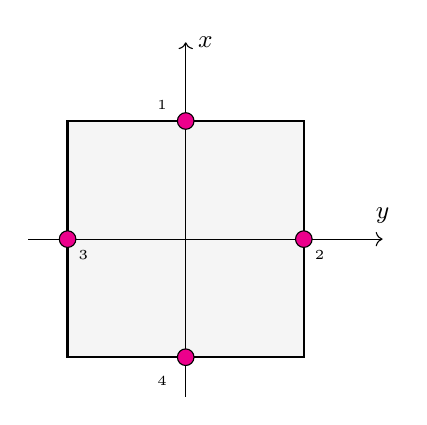
\begin{tikzpicture}
%\draw[step=1cm,gray,very thin] (0,0) grid (8,8); %background grid

\draw[thick,fill=gray!8] (1,1) -- (4,1) -- (4,4) -- (1,4) -- cycle;

\node[] at (1.2,2.3) {\tiny 3};
\node[] at (4.2,2.3) {\tiny 2};
\node[] at (2.2,.7) {\tiny 4};
\node[] at (2.2,4.2) {\tiny 1};

\draw[->] (0.5,2.5)--(5,2.5);
\draw[->] (2.5,0.5)--(2.5,5);

\draw[black,fill=magenta] (1,2.5)   circle (3pt);
\draw[black,fill=magenta] (4,2.5)   circle (3pt);
\draw[black,fill=magenta] (2.5,1)   circle (3pt);
\draw[black,fill=magenta] (2.5,4)   circle (3pt);

\node[] at (5,2.8) {\small $y$};
\node[] at (2.75,5) {\small $x$};
\end{tikzpicture}
\end{center}




\begin{verbatim}
+======3======+
|             |
|      s      |
|      |      |
4      +--r   2
|             |
|             |
|             |
+======1======+
\end{verbatim}

There are two types of basis functions: the Middle Point (MP) variant
such that $N_i({\bm r}_j)=\delta_{ij}$ and the Mid Value (MV) variant
such that $\frac{1}{|\Gamma_i|} \int_{\Gamma_i} N_j d\Gamma = \delta_{ij}$.

%.............................................
\paragraph{The Middle Point (MP) variant}. 
We have $\tilde{Q}_1=span \{ 1,r,s,r^2-s^2 \}$
so a function $f \in \tilde{Q}_1$  is such that 
\begin{equation}
f(r,s)= a + b r + c s + d(r^2-s^2 )
\label{nonpsf}
\end{equation}

This function must be so that 
\begin{eqnarray}
f_1 &=& f(r=0 ,s=-1) = a -c -d \\
f_2 &=& f(r=+1,s=0)  = a +b +d \\
f_3 &=& f(r=0 ,s=+1) = a +c -d \\
f_4 &=& f(r=-1,s=0)  = a -b +d 
\end{eqnarray}
and then 
\[
\left(
\begin{array}{c}
f_A \\ f_b \\ f_C \\ f_D
\end{array}
\right)
=
\left(
\begin{array}{cccc}
1 &0 &-1 &-1 \\
1 &1 &0 &1 \\
1 &0 &1 &-1 \\
1 &-1 &0 &1
\end{array}
\right)
\left(
\begin{array}{c}
a \\ b \\ c \\ d
\end{array}
\right)
\]
This system can easily be solved, $a,b,c,d$ are then replaced in Eq.~\eqref{nonpsf},
which yields 
\begin{eqnarray}
f(r,t) &=& N_1(r,s)f_1 +N_2(r,s)f_1 + N_3(r,s)f_3 +N_4(r,s)f_4
\end{eqnarray}
inside the element with
\begin{mdframed}[backgroundcolor=blue!5]
\begin{eqnarray}
N_1(r,s) &=& \frac{1}{4} (1-2s-(r^2-s^2)) \nonumber\\
N_2(r,s) &=& \frac{1}{4} (1+2r+(r^2-s^2)) \nonumber\\
N_3(r,s) &=& \frac{1}{4} (1+2s-(r^2-s^2)) \nonumber\\
N_4(r,s) &=& \frac{1}{4} (1-2r+(r^2-s^2)) \nonumber
\end{eqnarray}
\end{mdframed}
We of course recover the partition of unity property, i.e. $\sum N_i(r,s)=1$ for any coordinate $r,s$ inside 
the reference element.

\begin{remark}
These basis functions have been independently proposed by Donea \etal. \cite{dogm81}. The authors
prove herein that this element is checkerboard-free (although they do no show any example
of simulation carried out with this element).
\end{remark}

\begin{eqnarray}
\frac{\partial N_1}{\partial r} &=& \frac{1}{2}(-r)\\
\frac{\partial N_2}{\partial r} &=& \frac{1}{2}(1+r)\\
\frac{\partial N_3}{\partial r} &=& \frac{1}{2}(-r)\\
\frac{\partial N_4}{\partial r} &=& \frac{1}{2}(-1+r)
\end{eqnarray}

\begin{eqnarray}
\frac{\partial N_1}{\partial s} &=& \frac{1}{2}(-1+s)\\
\frac{\partial N_2}{\partial s} &=& \frac{1}{2}(-s)\\
\frac{\partial N_3}{\partial s} &=& \frac{1}{2}(1+s)\\
\frac{\partial N_4}{\partial s} &=& \frac{1}{2}(-s)
\end{eqnarray}

\begin{center}
\includegraphics[width=6cm]{images/rannacherturek/N1}
\includegraphics[width=6cm]{images/rannacherturek/N2}\\
\includegraphics[width=6cm]{images/rannacherturek/N3}
\includegraphics[width=6cm]{images/rannacherturek/N4}\\
{\captionfont Graphical representation of the $\tilde{Q}_1$ basis functions}
\end{center}

%......................................
\paragraph{The Mid Value (MV) variant}. 

These basis functions are implemented in deal.II
\footnote{\url{https://www.dealii.org/8.5.0/doxygen/deal.II/polynomials_rannacher_turek_8cc_source.html}}
for $x\in[0,1]$ and $y\in[0,1]$:

\begin{eqnarray}
N_1(x,y) &=&  0.75 + 1.5x - 2.5y -1.5(x^2-y^2) \quad bottom\\
N_2(x,y) &=& -0.25 - 0.5x + 1.5y +1.5(x^2-y^2) \quad right\\
N_3(x,y) &=& -0.25 + 1.5x - 0.5y -1.5(x^2-y^2) \quad top\\
N_4(x,y) &=&  0.75 - 2.5x + 1.5y +1.5(x^2-y^2) \quad left
\end{eqnarray}
We then proceed to rewrite these for $r\in[-1,1]$ and $t\in[-1:1]$:
\begin{mdframed}[backgroundcolor=blue!5]
\begin{eqnarray}
N_1(r,s) &=& \frac{1}{4} -\frac{1}{2}s - \frac{3}{8}(r^2-s^2) \quad bottom \\
N_2(r,s) &=& \frac{1}{4} +\frac{1}{2}r + \frac{3}{8}(r^2-s^2) \quad right \\
N_3(r,s) &=& \frac{1}{4} +\frac{1}{2}s - \frac{3}{8}(r^2-s^2) \quad top \\
N_4(r,s) &=& \frac{1}{4} -\frac{1}{2}r + \frac{3}{8}(r^2-s^2) \quad left
\end{eqnarray}
\end{mdframed}
It is easy to verify that these functions verify the property
\[
\frac{1}{|\Gamma_i|} \int_{\Gamma_i} N_j d\Gamma = \delta_{ij}
\]

These basis functions are used in \cite{shzh06} and mentioned in John \cite[p.722]{john16}.

\begin{eqnarray}
\frac{\partial N_1}{\partial r} &=& -\frac{3}{4}r \nonumber\\
\frac{\partial N_2}{\partial r} &=& \frac{1}{2}+\frac{3}{4}r \nonumber\\
\frac{\partial N_3}{\partial r} &=& -\frac{3}{4}r \nonumber\\
\frac{\partial N_4}{\partial r} &=& -\frac{1}{2}+\frac{3}{4}r \nonumber
\end{eqnarray}

\begin{eqnarray}
\frac{\partial N_1}{\partial t} &=& -\frac{1}{2}+\frac{3}{4}t \nonumber\\
\frac{\partial N_2}{\partial t} &=& -\frac{3}{4}t \nonumber\\
\frac{\partial N_3}{\partial t} &=& \frac{1}{2}+\frac{3}{4}t \nonumber\\
\frac{\partial N_4}{\partial t} &=& -\frac{3}{4}t \nonumber
\end{eqnarray}


\newpage
%-----------------------------------------------------------------------------
\subsubsection{The 2D enriched $Q_1^+\times P_0$ of Fortin} \label{ss:Q1pP02D}

We here consider the enriched $Q_1\times P_0$ element introduced first by 
Fortin (1981) \cite{fort81}.
The layout of the degrees of freedom is as follows:

\begin{flushright} {\tiny {\color{gray} (tikz\_q1pp02D.tex)}} \end{flushright}
%~~~~~~~~~~~~~~~~~~~~~~~~~~~~~~~~~~~~~~~~~~~~~~~~~~~~~~~~~~~~~~~~~~~~~~~~~~~~~~~~~~~~~~~~~~~~~~~~~~

\begin{center}
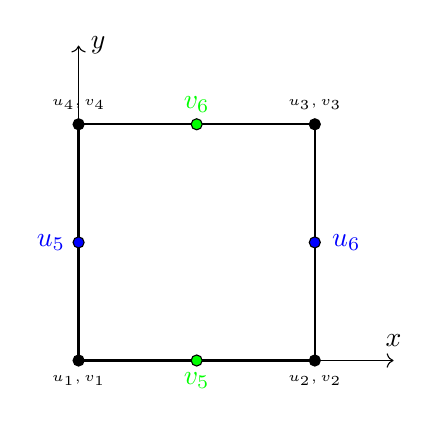
\begin{tikzpicture}
%\draw[fill=gray!23,gray!23](0,0) rectangle (6,5);
%\draw[step=0.5cm,gray,very thin] (0,0) grid (6,5); %background grid

\draw[thick] (1,.5) -- (4,.5) -- (4,3.5) -- (1,3.5) -- cycle; %front

\draw[thin,->] (4,0.5) -- (5,0.5); %x
\draw[thin,->] (1,3.5) -- (1,4.5); %y
\node[] at (5,0.75) {$x$};
\node[] at (1.25,4.5) {$y$};

\draw[black,fill=black] (1,.5)   circle (2pt);
\draw[black,fill=black] (4,.5)   circle (2pt);
\draw[black,fill=black] (4,3.5)   circle (2pt);
\draw[black,fill=black] (1,3.5)   circle (2pt);

\node[] at (1,0.25) {\tiny $u_1,v_1$};
\node[] at (4,0.25) {\tiny $u_2,v_2$};
\node[] at (4,3.75) {\tiny $u_3,v_3$};
\node[] at (1,3.75) {\tiny $u_4,v_4$};

\draw[black,fill=blue] (1,2) circle (2pt); 
\draw[black,fill=blue] (4,2) circle (2pt); 
\node[] at (0.65,2) {\color{blue} $u_5$};
\node[] at (4.4,2) {\color{blue} $u_{6}$};

\draw[black,fill=green] (2.5,0.5) circle (2pt); 
\draw[black,fill=green] (2.5,3.5) circle (2pt); 
\node[] at (2.5,0.25) {\color{green} $v_5$};
\node[] at (2.5,3.75) {\color{green} $v_{6}$};

\end{tikzpicture}\\
\end{center}


\noindent The approximation of the velocity components $u$ and $v$ inside the element is
\[
u^h(r,s) = a^u \; N_1(r,s) + b^u \;  N_2(r,s) + c^u \; N_3(r,s) +d^u \; N_4(r,s) 
+ d\; b_5^u(r,s) + e\; b_{6}^u(r,s)
\]
\[
v^h(r,s) = a^v \; N_1(r,s) + b^v \;  N_2(r,s) + c^v \; N_3(r,s) +d^v \; N_4(r,s) 
+ d^v b_5^v(r,s) + e^v b_{6}^v(r,s)
\]
where $N_{1,2,3,4}$ are the standard $Q_1$ basis functions in 2D and with 
\[
b_5^u(r,s) = \frac{1}{2}(1-r)(1-s^2)
\qquad
b_6^u(r,s) = \frac{1}{2}(1+r)(1-s^2)
\]
and
\[
b_5^v(r,s) = \frac{1}{2}(1-r^2)(1-s)
\qquad
b_6^v(r,s) = \frac{1}{2}(1-r^2)(1+s)
\]
In the end one arrives at

\begin{mdframed}[backgroundcolor=blue!5]
\begin{eqnarray}
{N}_1^u(r,s) &=&  N_1(r,s) - \frac{1}{2} b_5^u(r,s)\nn\\
{N}_2^u(r,s) &=&  N_2(r,s) - \frac{1}{2} b_6^u(r,s)\nn\\
{N}_3^u(r,s) &=&  N_3(r,s) - \frac{1}{2} b_6^u(r,s)\nn\\
{N}_4^u(r,s) &=&  N_4(r,s) - \frac{1}{2} b_5^u(r,s)\nn\\
{N}_5^u(r,s) &=&  b_5^u(r,s) \nn\\
{N}_6^u(r,s) &=&  b_6^u(r,s) \nn\\
\nn\\
{N}_1^v(r,s) &=&  N_1(r,s) - \frac{1}{2} b_5^v(r,s)\nn\\
{N}_2^v(r,s) &=&  N_2(r,s) - \frac{1}{2} b_5^v(r,s)\nn\\
{N}_3^v(r,s) &=&  N_3(r,s) - \frac{1}{2} b_6^v(r,s)\nn\\
{N}_4^v(r,s) &=&  N_4(r,s) - \frac{1}{2} b_6^v(r,s)\nn\\
{N}_5^v(r,s) &=&  b_5^v(r,s) \nn\\
{N}_6^v(r,s) &=&  b_6^v(r,s) 
\end{eqnarray}
\end{mdframed}

We can check for the zero-th order consistency: Let $u(r,s)=C$, then 
\begin{eqnarray}
u^h(r,s) 
= \sum_{i=1}^6 N_i^u(r,s) u_i 
= C \sum_{i=1}^6 N_i^u(r,s) 
= C \sum_{i=1}^4 N_i(r,s)  
= C
\end{eqnarray}



\newpage
%-----------------------------------------------------------------------------
\subsubsection{The DSSY element} \label{ss:dssy_2D}
This element is often reffered to as the 'DSSY' element becaus of the 
four authors of the original paper: Douglas, Santos, sheen and Ye (1999) \cite{doss99}.

The non-conforming finite element space i$Q_l$ is defined based on the 
reference square element on $[-1,1]^2$ :
\[
Q_l = \text{Span} \left\{ 1, r, s, \theta_l(r)-\theta_l(s)  \right\}
\qquad l=1,\; \text{or} \; 2
\]
with
\begin{eqnarray}
\theta_1(r)  &=& r^2-\frac53r^4  \nn\\
\theta_1'(r) &=& 2r-\frac{20}{3}r^3  \nn\\
\theta_2(r)  &=& r^2-\frac{25}{6} r^4 + \frac72 r^6 \\ 
\theta_2'(r) &=& 2r-\frac{50}{3} r^3 + 21 r^5
\end{eqnarray}
The dimension of $Q_l$ is four and the $\theta_l$ functions look like:
\begin{center}
\includegraphics[width=7cm]{images/dssy/theta1}
\includegraphics[width=7cm]{images/dssy/theta2}
\end{center}
We have:
\begin{itemize}
\item $\theta_1(r=-1)=\theta_1(r=+1)=-\frac23$, $\theta_1(r=0)=0$ 
\item $\theta_2(r=-1)=\theta_2(r=+1)=\frac13$, $\theta_2(r=0)=0$ 
\end{itemize}
The nodes are situated at the mid-edges of the quadrilateral:

\input{tikz_dssy2D}

The basis function corresponding to the node (1, 0) is given by
\begin{mdframed}[backgroundcolor=blue!5]
\begin{eqnarray}
N_1(r,s)^{(l)} &=& \frac{1}{4} - \frac{1}{2} r + \frac{\theta_l(r)-\theta_l(s)}{4 \theta_l(1)}  \nn\\
N_2(r,s)^{(l)} &=& \frac{1}{4} + \frac{1}{2} r + \frac{\theta_l(r)-\theta_l(s)}{4 \theta_l(1)}  \nn\\
N_3(r,s)^{(l)} &=& \frac{1}{4} - \frac{1}{2} s - \frac{\theta_l(r)-\theta_l(s)}{4 \theta_l(1)}  \nn\\
N_4(r,s)^{(l)} &=& \frac{1}{4} + \frac{1}{2} s - \frac{\theta_l(r)-\theta_l(s)}{4 \theta_l(1)}  
\end{eqnarray}
\end{mdframed}
We can easily verify that $\sum_i N_i(r,s,t)=1$ and that $N_i(\vec{r}_j)=\delta_{ij}$:
\begin{eqnarray}
N_1^{(l)}(r_1,s_1) 
&=& \frac{1}{4} -\frac{1}{2} (-1) + \frac{\theta_l(-1)-\theta_l(0)}{4 \theta_l(1)}  
= \frac{1}{4} +\frac{1}{2}  + \frac{\theta_l(-1)}{4 \theta_l(1)}  
= \frac{1}{4} +\frac{1}{2}  + \frac{1}{4}   = 1 \nn\\
N_1^{(l)}(r_2,s_2)
&=& \frac{1}{4} -\frac{1}{2} (+1) + \frac{\theta_l(+1)-\theta_l(0)}{4 \theta_l(1)}  
= \frac{1}{4} -\frac{1}{2} + \frac{\theta_l(+1)}{4 \theta_l(1)}  
= \frac{1}{4} -\frac{1}{2} + \frac{1}{4}   = 0 \nn\\
N_1^{(l)}(r_3,s_3)
&=& \frac{1}{4} -\frac{1}{2} (0) + \frac{\theta_l(0)-\theta_l(-1)}{4 \theta_l(1)}  
= \frac14 -\frac14  = 0 \nn\\
N_1^{(l)}(r_4,s_4)
&=& \frac{1}{4} -\frac{1}{2} (0) + \frac{\theta_l(0)-\theta_l(+1)}{4 \theta_l(1)}  
= \frac14 -\frac14  = 0 \nn\\
N_2^{(l)}(r_1,s_1) 
&=& \frac{1}{4} + \frac{1}{2} (-1) + \frac{\theta_l(-1)-\theta_l(0)}{4 \theta_l(1)}  
= \frac14 -\frac12 + \frac14 = 0 \nn\\
N_2^{(l)}(r_2,s_2)
&=& \frac{1}{4} + \frac{1}{2} (+1) + \frac{\theta_l(+1)-\theta_l(0)}{4 \theta_l(1)}  
= \frac14 + \frac12 + \frac14 =1 \nn\\
N_2^{(l)}(r_3,s_3)
&=& \frac{1}{4} + \frac{1}{2} (0) + \frac{\theta_l(0)-\theta_l(-1)}{4 \theta_l(1)}  
= \frac14 - \frac14 = 0 \nn\\
N_2^{(l)}(r_4,s_4)
&=& \frac{1}{4} + \frac{1}{2} (0) + \frac{\theta_l(0)-\theta_l(+1)}{4 \theta_l(1)}  
= \frac14 - \frac14 = 0 \nn\\
N_3^{(l)}(r_1,s_1)
&=& \frac{1}{4} - \frac{1}{2} (0) - \frac{\theta_l(-1)-\theta_l(0)}{4 \theta_l(1)} 
= \frac14 -\frac14 = 0\nn\\
N_3^{(l)}(r_2,s_2)
&=& \frac{1}{4} - \frac{1}{2} (0) - \frac{\theta_l(+1)-\theta_l(0)}{4 \theta_l(1)} 
= \frac14 -\frac14 = 0\nn\\
N_3^{(l)}(r_3,s_3)
&=& \frac{1}{4} - \frac{1}{2} (-1) - \frac{\theta_l(0)-\theta_l(-1)}{4 \theta_l(1)} 
= \frac14 +\frac12 + \frac14 = 1\nn\\
N_3^{(l)}(r_4,s_4)
&=& \frac{1}{4} - \frac{1}{2} (+1) - \frac{\theta_l(0)-\theta_l(+1)}{4 \theta_l(1)} 
= \frac14 -\frac12 + \frac14 = 0\nn\\
N_4^{(l)}(r_1,s_1)
&=& \frac{1}{4} + \frac{1}{2} (0) - \frac{\theta_l(-1)-\theta_l(0)}{4 \theta_l(1)}  
= \frac14 -\frac14 =0\nn\\
N_4^{(l)}(r_2,s_2)
&=& \frac{1}{4} + \frac{1}{2} (0) - \frac{\theta_l(+1)-\theta_l(0)}{4 \theta_l(1)}  
= \frac14 -\frac14 =0\nn\\
N_4^{(l)}(r_3,s_3)
&=& \frac{1}{4} + \frac{1}{2} (-1) - \frac{\theta_l(0)-\theta_l(-1)}{4 \theta_l(1)}  
= \frac14 -\frac12 +\frac14 = 0 \nn\\
N_4^{(l)}(r_4,s_4)
&=& \frac{1}{4} + \frac{1}{2} (1) - \frac{\theta_l(0)-\theta_l(1)}{4 \theta_l(1)}  
= \frac14 +\frac12 +\frac14 = 1 \nn
\end{eqnarray}

The basis functions can also be explicitely written for $\theta_1$ as in Cai \etal \cite{cady99}:
\begin{eqnarray}
N_1(r,s)^{(l)} 
&=& \frac{1}{4} - \frac{1}{2} r - \frac38 \left[\left( r^2-\frac53r^4 \right) - \left(s^2-\frac53s^4 \right) \right] \nn\\
N_2(r,s)^{(l)} 
&=& \frac{1}{4} + \frac{1}{2} r - \frac38 \left[\left( r^2-\frac53r^4 \right) - \left(s^2-\frac53s^4 \right) \right] \nn\\
N_3(r,s)^{(l)} 
&=& \frac{1}{4} - \frac{1}{2} s + \frac38 \left[\left( r^2-\frac53r^4 \right) - \left(s^2-\frac53s^4 \right) \right] \nn\\
N_4(r,s)^{(l)} 
&=& \frac{1}{4} + \frac{1}{2} s + \frac38 \left[\left( r^2-\frac53r^4 \right) - \left(s^2-\frac53s^4 \right) \right] 
\end{eqnarray}

The derivatives of the basis functions are as follows:
\begin{eqnarray}
\partial_r N_1(r,s)^{(l)} &=&  - \frac{1}{2}  + \frac{\theta_l'(r)}{4 \theta_l(1)}  \nn\\
\partial_r N_2(r,s)^{(l)} &=&  + \frac{1}{2}  + \frac{\theta_l'(r)}{4 \theta_l(1)}  \nn\\
\partial_r N_3(r,s)^{(l)} &=&  - \frac{\theta_l'(r)}{4 \theta_l(1)}  \nn\\
\partial_r N_4(r,s)^{(l)} &=&  - \frac{\theta_l'(r)}{4 \theta_l(1)}  
\end{eqnarray}

\begin{eqnarray}
\partial_s N_1(r,s)^{(l)} &=&   -\frac{\theta_l'(s)}{4 \theta_l(1)}  \nn\\
\partial_s N_2(r,s)^{(l)} &=&   -\frac{\theta_l'(s)}{4 \theta_l(1)}  \nn\\
\partial_s N_3(r,s)^{(l)} &=&   - \frac{1}{2} + \frac{\theta_l'(s)}{4 \theta_l(1)}  \nn\\
\partial_s N_4(r,s)^{(l)} &=&   + \frac{1}{2} + \frac{\theta_l'(s)}{4 \theta_l(1)}  
\end{eqnarray}





\Literature: 
Jeon \etal (2013) \cite{jens13},
Bangerth \etal (2017) \cite{baks17},
Sheen (2020) \cite{shee20}













 %-----------
\newpage
\section{Elements and basis functions in 3D} 

%%%%%%%%%%%%%%%%%%%%%%%%%%%%%%%%%%%%%%%%%%%%%%%%%%%%%%%
\subsubsection{Linear basis functions in tetrahedra ($P_1$)}
\index{$P_1$}


\begin{verbatim}
(r_0,s_0) = (0,0,0)
(r_1,s_1) = (1,0,0)
(r_2,s_2) = (0,2,0)
(r_3,s_3) = (0,0,1)
\end{verbatim}

The basis polynomial is given by
\[
f(r,s,t)=c_0 + c_1 r + c_2 s + c_3 t
\]

\begin{eqnarray}
f_1 &=& f(r_1,s_1,t_1) = c_0 \\
f_2 &=& f(r_2,s_2,t_2) = c_0 + c_1\\
f_3 &=& f(r_3,s_3,t_3) = c_0 + c_2\\
f_4 &=& f(r_4,s_4,t_4) = c_0 + c_3
\end{eqnarray}

which yields:
\[
c_0=f_1
\quad
\quad
c_1=f_2-f_1
\quad
\quad
c_2=f_3-f_1
\quad
\quad
c_3=f_4-f_1
\]

\begin{eqnarray}
f(r,s,t) 
&=& c_0 + c_1 r + c_2 s + c_3 t \nonumber\\
&=& f_1 + (f_2-f_1) r + (f_3-f_1) s + (f_4-f_1) t \nonumber\\
&=& f_1 (1-r-s-t) + f_2 r + f_3 s + f_4 t \nonumber\\
&=& \sum_i N_i(r,s,t) f_i \nonumber
\end{eqnarray}

Finally,

\begin{mdframed}[backgroundcolor=blue!5]
\begin{eqnarray}
N_1(r,s,t) &=& 1-r-s-t \nonumber\\
N_2(r,s,t) &=& r \nonumber\\
N_3(r,s,t) &=& s \nonumber\\
N_4(r,s,t) &=& t \nonumber
\end{eqnarray}
\end{mdframed}









%%%%%%%%%%%%%%%%%%%%%%%%%%%%%%%%%%%%%%%%%%%%%%%%%%%%%%%
\subsubsection{Triquadratic basis functions in 3D ($Q_2$)}
\index{$Q_2$}

\begin{eqnarray}
N_{1}&=& 0.5r(r-1)  \;0.5s(s-1)\; 0.5t(t-1)  \nonumber\\
N_{2}&=& 0.5r(r+1)  \;0.5s(s-1)\; 0.5t(t-1)  \nonumber\\
N_{3}&=& 0.5r(r+1)  \;0.5s(s+1)\; 0.5t(t-1)  \nonumber\\
N_{4}&=& 0.5r(r-1)  \;0.5s(s+1)\; 0.5t(t-1)  \nonumber\\
N_{5}&=& 0.5r(r-1)  \;0.5s(s-1)\; 0.5t(t+1)  \nonumber\\
N_{6}&=& 0.5r(r+1)  \;0.5s(s-1)\; 0.5t(t+1)  \nonumber\\
N_{7}&=& 0.5r(r+1)  \;0.5s(s+1)\; 0.5t(t+1)  \nonumber\\
N_{8}&=& 0.5r(r-1)  \;0.5s(s+1)\; 0.5t(t+1)  \nonumber\\
N_{9}&=& (1.-r^2)   \;0.5s(s-1)\; 0.5t(t-1)  \nonumber\\
N_{10}&=& 0.5r(r+1) \;(1-s^2)  \; 0.5t(t-1)  \nonumber\\
N_{11}&=& (1.-r^2)  \;0.5s(s+1)\; 0.5t(t-1)  \nonumber\\
N_{12}&=& 0.5r(r-1) \;(1-s^2)  \; 0.5t(t-1)  \nonumber\\
N_{13}&=& (1.-r^2)  \;0.5s(s-1)\; 0.5t(t+1)  \nonumber\\
N_{14}&=& 0.5r(r+1) \;(1-s^2)  \; 0.5t(t+1)  \nonumber\\
N_{15}&=& (1.-r^2)  \;0.5s(s+1)\; 0.5t(t+1)  \nonumber\\
N_{16}&=& 0.5r(r-1) \;(1-s^2)  \; 0.5t(t+1)  \nonumber\\
N_{17}&=& 0.5r(r-1) \;0.5s(s-1)\; (1-t^2)  \nonumber\\
N_{18}&=& 0.5r(r+1) \;0.5s(s-1)\; (1-t^2)  \nonumber\\
N_{19}&=& 0.5r(r+1) \;0.5s(s+1)\; (1-t^2)  \nonumber\\
N_{20}&=& 0.5r(r-1) \;0.5s(s+1)\; (1-t^2)  \nonumber\\
N_{21}&=& (1-r^2)   \;(1-s^2)  \; 0.5t(t-1)  \nonumber\\
N_{22}&=& (1-r^2)   \;0.5s(s-1)\; (1-t^2)  \nonumber\\
N_{23}&=& 0.5r(r+1) \;(1-s^2)  \; (1-t^2)  \nonumber\\
N_{24}&=& (1-r^2)   \;0.5s(s+1)\; (1-t^2)  \nonumber\\
N_{25}&=& 0.5r(r-1) \;(1-s^2)  \; (1-t^2)  \nonumber\\
N_{26}&=& (1-r^2)   \;(1-s^2)  \; 0.5t(t+1)  \nonumber\\
N_{27}&=& (1-r^2)   \;(1-s^2)  \; (1-t^2)  \nonumber
\end{eqnarray}

 %-------------------------------
\newpage
\section{Low order elements recap} Let us assume a Cartesian domain discretised in $nel_x \times nel_y$
elements in 2D and $nel_x \times nel_y \times nel_z$ elements in 3D.
Focusing only on the total number of velocity dofs (the values indicated after the 
arrows are the limits when $nel_x=nel_y=nel_z >> 1$):

\begin{itemize}

\item $Q_1 \times P_0$, $Q_1 \times Q_1$
\begin{align}
ndof_{2D}&= 2 (nel_x+1) \cdot (nel_y+1) 
& \rightarrow  2 \cdot nel_x^2   \\
ndof_{3D}&= 3 (nel_x+1) \cdot (nel_y+1) \cdot (nel_z+1)
& \rightarrow 3 \cdot nel_x^3 
\end{align}

\item $Q_2 \times P_{-1}$, $Q_2 \times Q_1$
\begin{eqnarray}
ndof_{2D}      &=&2 (2nel_x+1) \cdot (2nel_y+1) 
\qquad \rightarrow \qquad 8 \cdot nel_x^2   \nonumber\\
ndof_{3D}&=&3 (2nel_x+1) \cdot (2nel_y+1) \cdot (2nel_z+1)
\qquad \rightarrow \qquad 24 \cdot nel_x^3 \nonumber
\end{eqnarray}


\item $Q_1^+ \times P_0$

\begin{eqnarray}
ndof_{2D}     &=&2 (nel_x+1) \cdot (nel_y+1) + (nel_x+1)\cdot nel_y + nel_x\cdot(nel_y+1)
\qquad \rightarrow \qquad 4 \cdot nel_x^2   \nonumber\\
ndof_{3D}&=&3 (nel_x+1) \cdot (nel_y+1) \cdot (nel_z+1) \nonumber\\
&+&  (nel_x+1)\cdot nel_y \cdot nel_z + nelx\cdot (nel_y+1) \cdot nelz + nelx\cdot nely \cdot (nel_z+1)
\quad \rightarrow \quad 6 \cdot nel_x^3 \nonumber
\end{eqnarray}

\item $Q_1 \times Q_1$+1 bubble

\begin{eqnarray}
ndof_{2D}&=& 2[(nel_x+1) \cdot (nel_y+1)  + \cdot nelx\cdot nely ]
\quad \rightarrow \quad 4 \cdot nel_x^2 \nonumber
\end{eqnarray}

%\item $Q_1^+ \times Q_1$
%\begin{eqnarray}
%ndof_{2D}  &=&2 [ (nel_x+1) \cdot (nel_y+1) + nel_x \cdot nel_y ]
%\qquad \rightarrow \qquad 4 \cdot nel_x^2   \nonumber
%ndof_{3D}  &=&3 [ (nel_x+1) \cdot (nel_y+1) \cdot (nel_z+1) + nel_x \cdot nel_y \cdot nel_z ]
%\qquad \rightarrow \qquad 6 \cdot nel_x^3 \nonumber
%\end{eqnarray}

\item $Q_1 \times Q_1$+2 bubbles

\begin{eqnarray}
ndof_{3D}&=& 3[(nel_x+1) \cdot (nel_y+1) \cdot  (nel_z+1) + 2\cdot nelx\cdot nely \cdot nelz]
\quad \rightarrow \quad 9 \cdot nel_x^3 \nonumber
\end{eqnarray}


\item Rannacher-turek or DSSY:

\begin{eqnarray}
ndof_{2D}&=& 2[(nel_y+1) \cdot nel_x+nel_y\cdot(nel_x+1)  ] 
\quad\rightarrow \quad 4 \cdot nel_x^2 \nonumber\nn\\
ndof_{3D}&=& 3[ nel_x\cdot (nel_y+1)\cdot nel_z + (nel_x+1) \cdot nel_y\cdot nel_z  +nel_x\cdot nel_y\cdot (nel_z+1) ]  
\quad \rightarrow \quad 9 \cdot nel_x^3 \nonumber
\end{eqnarray}
 

\end{itemize}


If we now assume $nel_x=nel_y=nel_z$, we can then plot the values above as a function of $nel_x$:
\begin{center}
\includegraphics[width=7.5cm]{images/elements/ndof2D.pdf}
\includegraphics[width=7.5cm]{images/elements/ndof3D.pdf}
\end{center}

We see that the $Q_1^+\times Q_1$ and $Q_1^+ \times P_0$ actually 
yield the same number of velocity dofs. 

Simply based on the dof count and wishing for a (bi/tri)linear approximation 
for pressure, we must conclude that the $Q_1\times Q_1$+2 bubbles is the most desirable 
since it is also LBB stable.

\begin{center}
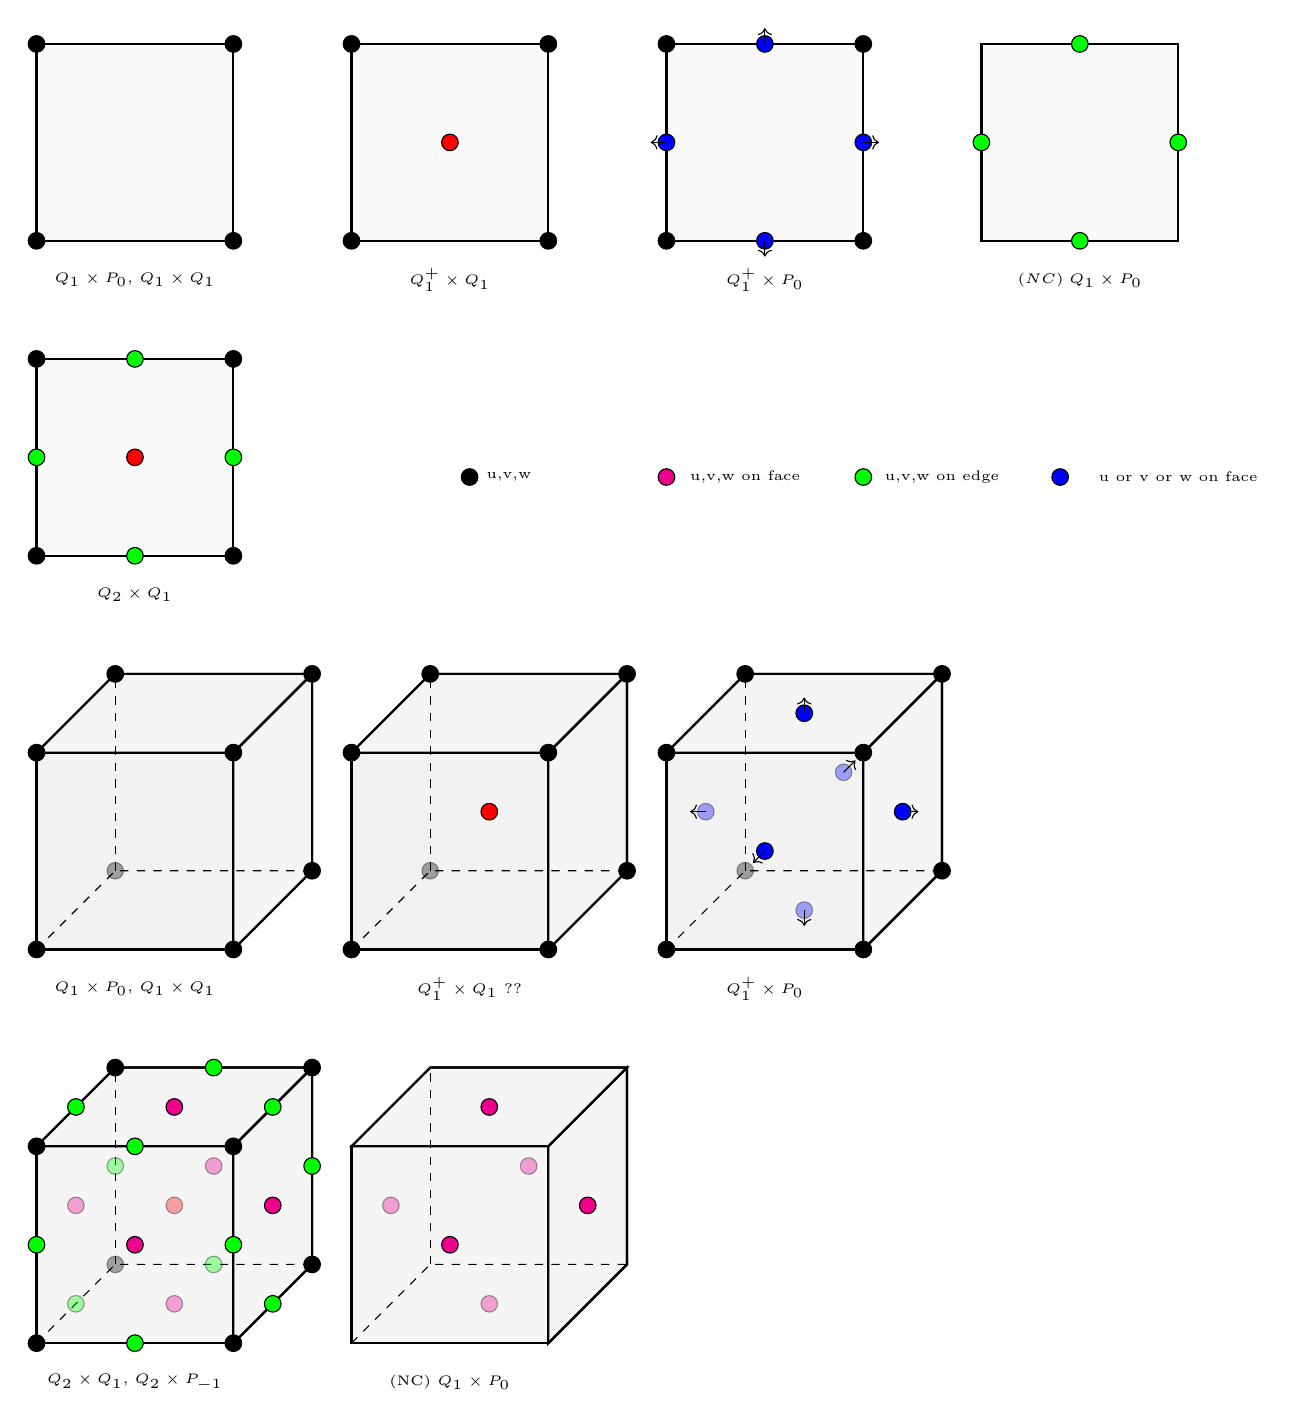
\begin{tikzpicture}
%\draw[fill=gray!23,gray!23](0,0) rectangle (20,10);
%\draw[step=0.5cm,gray,very thin] (0,0) grid (18,18); %background grid

%%%%%%%%%%%%%%%%%%%%%%%%%%%%%%%%%%%%%%%%%%%%%%%%%%%%%%%%%%%%%%%%%%%%
%bottom row
%%%%%%%%%%%%%%%%%%%%%%%%%%%%%%%%%%%%%%%%%%%%%%%%%%%%%%%%%%%%%%%%%%%%
\draw[thick,fill=gray!8] (1,1) -- (3.5,1) -- (3.5,3.5) -- (1,3.5) -- cycle;
\draw[thick,fill=gray!8] (5,1) -- (7.5,1) -- (7.5,3.5) -- (5,3.5) -- cycle;
%\draw[thick,fill=gray!8] (9,1) -- (11.5,1) -- (11.5,3.5) -- (9,3.5) -- cycle;
%\draw[thick,fill=gray!8] (13,1) -- (15.5,1) -- (15.5,3.5) -- (13,3.5) -- cycle;

%right sides
\draw[thick,fill=gray!8] (3.5,1) -- (4.5,2) -- (4.5,4.5) -- (3.5,3.5) -- cycle;
\draw[thick,fill=gray!8] (7.5,1) -- (8.5,2) -- (8.5,4.5) -- (7.5,3.5) -- cycle;
%\draw[thick,fill=gray!8] (11.5,1) -- (12.5,2) -- (12.5,4.5) -- (11.5,3.5) -- cycle;
%\draw[thick,fill=gray!8] (15.5,1) -- (16.5,2) -- (16.5,4.5) -- (15.5,3.5) -- cycle;

%tops
\draw[thick,fill=gray!8] (1,3.5) -- (3.5,3.5) -- (4.5,4.5) -- (2,4.5) -- cycle;
\draw[thick,fill=gray!8] (5,3.5) -- (7.5,3.5) -- (8.5,4.5) -- (6,4.5) -- cycle;
%\draw[thick,fill=gray!8] (9,3.5) -- (11.5,3.5) -- (12.5,4.5) -- (10,4.5) -- cycle;
%\draw[thick,fill=gray!8] (13,3.5) -- (15.5,3.5) -- (16.5,4.5) -- (14,4.5) -- cycle;

\draw[thick] (1,3.5) -- (2,4.5) -- (4.5,4.5) -- (4.5,2) -- (3.5,1);
\draw[thick] (5,3.5) -- (6,4.5) -- (8.5,4.5) -- (8.5,2) -- (7.5,1);
%\draw[thick] (9,3.5) -- (10,4.5) -- (12.5,4.5) -- (12.5,2) -- (11.5,1);
%\draw[thick] (13,3.5) -- (14,4.5) -- (16.5,4.5) -- (16.5,2) -- (15.5,1);

\draw[thick] (3.5,3.5) -- (4.5,4.5) ;
\draw[thick] (7.5,3.5) -- (8.5,4.5) ;
%\draw[thick] (11.5,3.5) -- (12.5,4.5) ;
%\draw[thick] (15.5,3.5) -- (16.5,4.5) ;

\draw[dashed] (1,1) -- (2,2) -- (4.5,2) ;\draw[dashed] (2,2) -- (2,4.5);
\draw[dashed] (5,1) -- (6,2) -- (8.5,2) ;\draw[dashed] (6,2) -- (6,4.5);
%\draw[dashed] (9,1) -- (10,2) -- (12.5,2) ;\draw[dashed] (10,2) -- (10,4.5);
%\draw[dashed] (13,1) -- (14,2) -- (16.5,2) ;\draw[dashed] (14,2)--(14,4.5);

\draw[black,fill=black] (1,1)   circle (3pt);
\draw[black,fill=black] (3.5,1)   circle (3pt);
\draw[black,fill=black] (3.5,3.5)   circle (3pt);
\draw[black,fill=black] (1,3.5)   circle (3pt);
\draw[black,fill=black] (2,4.5)   circle (3pt);
\draw[black,fill=black] (4.5,4.5)   circle (3pt);
\draw[black,fill=black] (4.5,2)   circle (3pt);
\draw[black,fill=black,opacity=0.35] (2,2)   circle (3pt);

%\draw[black,fill=black] (5,1)   circle (3pt);
%\draw[black,fill=black] (7.5,1)   circle (3pt);
%\draw[black,fill=black] (7.5,3.5)   circle (3pt);
%\draw[black,fill=black] (5,3.5)   circle (3pt);
%\draw[black,fill=black] (6,4.5)   circle (3pt);
%\draw[black,fill=black] (8.5,4.5)   circle (3pt);
%\draw[black,fill=black] (8.5,2)   circle (3pt);
%\draw[black,fill=black,opacity=0.35] (6,2)   circle (3pt);

%\draw[black,fill=black] (9,1)   circle (3pt);
%\draw[black,fill=black] (11.5,1)   circle (3pt);
%\draw[black,fill=black] (11.5,3.5)   circle (3pt);
%\draw[black,fill=black] (9,3.5)   circle (3pt);
%\draw[black,fill=black] (10,4.5)   circle (3pt);
%\draw[black,fill=black] (12.5,4.5)   circle (3pt);
%\draw[black,fill=black] (12.5,2)   circle (3pt);
%\draw[black,fill=black,opacity=0.35] (10,2)   circle (3pt);

%\draw[black,fill=black] (13,1)   circle (3pt);
%\draw[black,fill=black] (15.5,1)   circle (3pt);
%\draw[black,fill=black] (15.5,3.5)   circle (3pt);
%\draw[black,fill=black] (13,3.5)   circle (3pt);
%\draw[black,fill=black] (14,4.5)   circle (3pt);
%\draw[black,fill=black] (16.5,4.5)   circle (3pt);
%\draw[black,fill=black] (16.5,2)   circle (3pt);
%\draw[black,fill=black,opacity=0.35] (14,2)   circle (3pt);


%%%%%%%%%%%%%%%%%%%%%%%%%%%%%%%%%%%%%%%%%%%%%%%%%%%%%%%%%%%%%%%%%%%%
%3rd row 
%%%%%%%%%%%%%%%%%%%%%%%%%%%%%%%%%%%%%%%%%%%%%%%%%%%%%%%%%%%%%%%%%%%%

\draw[thick,fill=gray!5] (1,15) -- (3.5,15) -- (3.5,17.5) -- (1,17.5) -- cycle;
\draw[thick,fill=gray!5] (5,15) -- (7.5,15) -- (7.5,17.5) -- (5,17.5) -- cycle;
\draw[thick,fill=gray!5] (9,15) -- (11.5,15) -- (11.5,17.5) -- (9,17.5) -- cycle;
\draw[thick,fill=gray!5] (13,15) -- (15.5,15) -- (15.5,17.5) -- (13,17.5) -- cycle;

\draw[black,fill=black] (1,15)   circle (3pt);
\draw[black,fill=black] (3.5,15)   circle (3pt);
\draw[black,fill=black] (1,17.5)   circle (3pt);
\draw[black,fill=black] (3.5,17.5)   circle (3pt);
\node[] at (2.25,14.5) {\tiny $Q_1\times P_0$, $Q_1\times Q_1$};


\draw[black,fill=black] (5,15)   circle (3pt);
\draw[black,fill=black] (7.5,15)   circle (3pt);
\draw[black,fill=black] (5,17.5)   circle (3pt);
\draw[black,fill=black] (7.5,17.5)   circle (3pt);
\node[] at (6.25,14.5) {\tiny $Q_1^+\times Q_1$};
\draw[black,fill=red] (6.25,16.25)   circle (3pt);

\draw[black,fill=black] (9,15)   circle (3pt);
\draw[black,fill=black] (11.5,15)   circle (3pt);
\draw[black,fill=black] (9,17.5)   circle (3pt);
\draw[black,fill=black] (11.5,17.5)   circle (3pt);
\node[] at (10.25,14.5) {\tiny $Q_1^+\times P_0$};

\draw[black,fill=blue] (9,16.25)   circle (3pt);
\draw[black,fill=blue] (11.5,16.25)   circle (3pt);
\draw[black,fill=blue] (10.25,15)   circle (3pt);
\draw[black,fill=blue] (10.25,17.5)   circle (3pt);

\draw[fill=blue,->] (9,16.25) -- (8.8,16.25); 
\draw[fill=blue,->] (11.5,16.25) -- (11.7,16.25); 
\draw[fill=blue,->] (10.25,15) -- (10.25,14.8); 
\draw[fill=blue,->] (10.25,17.5) -- (10.25,17.7); 


\draw[black,fill=green] (14.25,15)   circle (3pt);
\draw[black,fill=green] (14.25,17.5)   circle (3pt);
\draw[black,fill=green] (13,16.25)   circle (3pt);
\draw[black,fill=green] (15.5,16.25)   circle (3pt);
\node[] at (14.25,14.5) {\tiny $(NC)\; Q_1\times P_0$};

%%%%%%%%%%%%%%%%%%%%%%%%%%%%%%%%%%%%%%%%%%%%%%%%%%%%%%%%%%%%%%%%%%%%
%2nd row 
%%%%%%%%%%%%%%%%%%%%%%%%%%%%%%%%%%%%%%%%%%%%%%%%%%%%%%%%%%%%%%%%%%%%

\draw[thick,fill=gray!5] (1,11) -- (3.5,11) -- (3.5,13.5) -- (1,13.5) -- cycle;
%\draw[thick,fill=gray!5] (5,11) -- (7.5,11) -- (7.5,13.5) -- (5,13.5) -- cycle;
%\draw[thick,fill=gray!5] (9,11) -- (11.5,11) -- (11.5,13.5) -- (9,13.5) -- cycle;
%\draw[thick,fill=gray!5] (13,11) -- (15.5,11) -- (15.5,13.5) -- (13,13.5) -- cycle;

\draw[black,fill=black] (1,11)   circle (3pt);
\draw[black,fill=green] (2.25,11)   circle (3pt);
\draw[black,fill=black] (3.5,11)   circle (3pt);
\draw[black,fill=green] (1,12.25)   circle (3pt);
\draw[black,fill=red] (2.25,12.25)   circle (3pt);
\draw[black,fill=green] (3.5,12.25)   circle (3pt);
\draw[black,fill=black] (1,13.5)   circle (3pt);
\draw[black,fill=green] (2.25,13.5)   circle (3pt);
\draw[black,fill=black] (3.5,13.5)   circle (3pt);
\node[] at (2.25,10.5) {\tiny $Q_2\times Q_1$};



%%%%%%%%%%%%%%%%%%%%%%%%%%%%%%%%%%%%%%%%%%%%%%%%%%%%%%%%%%%%%%%%%%%%
%1st row 
%%%%%%%%%%%%%%%%%%%%%%%%%%%%%%%%%%%%%%%%%%%%%%%%%%%%%%%%%%%%%%%%%%%%
\draw[thick,fill=gray!10] (1,6) -- (3.5,6) -- (3.5,8.5) -- (1,8.5) -- cycle;
\draw[thick,fill=gray!10] (5,6) -- (7.5,6) -- (7.5,8.5) -- (5,8.5) -- cycle;
\draw[thick,fill=gray!10] (9,6) -- (11.5,6) -- (11.5,8.5) -- (9,8.5) -- cycle;
%\draw[thick,fill=gray!10] (13,6) -- (15.5,6) -- (15.5,8.5) -- (13,8.5) -- cycle;

%right sides
\draw[thick,fill=gray!8] (3.5,6) -- (4.5,7) -- (4.5,9.5) -- (3.5,8.5) -- cycle;
\draw[thick,fill=gray!8] (7.5,6) -- (8.5,7) -- (8.5,9.5) -- (7.5,8.5) -- cycle;
\draw[thick,fill=gray!8] (11.5,6) -- (12.5,7) -- (12.5,9.5) -- (11.5,8.5) -- cycle;
%\draw[thick,fill=gray!8] (15.5,6) -- (16.5,7) -- (16.5,9.5) -- (15.5,8.5) -- cycle;

%tops
\draw[thick,fill=gray!8] (1,8.5) -- (3.5,8.5) -- (4.5,9.5) -- (2,9.5) -- cycle;
\draw[thick,fill=gray!8] (5,8.5) -- (7.5,8.5) -- (8.5,9.5) -- (6,9.5) -- cycle;
\draw[thick,fill=gray!8] (9,8.5) -- (11.5,8.5) -- (12.5,9.5) -- (10,9.5) -- cycle;
%\draw[thick,fill=gray!8] (13,8.5) -- (15.5,8.5) -- (16.5,9.5) -- (14,9.5) -- cycle;


\draw[thick] (1,8.5) -- (2,9.5) -- (4.5,9.5) -- (4.5,7) -- (3.5,6);
\draw[thick] (5,8.5) -- (6,9.5) -- (8.5,9.5) -- (8.5,7) -- (7.5,6);
\draw[thick] (9,8.5) -- (10,9.5) -- (12.5,9.5) -- (12.5,7) -- (11.5,6);
%\draw[thick] (13,8.5) -- (14,9.5) -- (16.5,9.5) -- (16.5,7) -- (15.5,6);

\draw[thick] (3.5,8.5) -- (4.5,9.5) ;
\draw[thick] (7.5,8.5) -- (8.5,9.5) ;
\draw[thick] (11.5,8.5) -- (12.5,9.5) ;
%\draw[thick] (15.5,8.5) -- (16.5,9.5) ;

\draw[dashed] (1,6) -- (2,7) -- (4.5,7)    ;\draw[dashed] (2,7) -- (2,9.5);
\draw[dashed] (5,6) -- (6,7) -- (8.5,7)    ;\draw[dashed] (6,7) -- (6,9.5);
\draw[dashed] (9,6) -- (10,7) -- (12.5,7)  ;\draw[dashed] (10,7) -- (10,9.5);
%\draw[dashed] (13,6) -- (14,7) -- (16.5,7) ;\draw[dashed] (14,7) -- (14,9.5);

\draw[black,fill=black] (1,6)   circle (3pt);
\draw[black,fill=black] (3.5,6)   circle (3pt);
\draw[black,fill=black] (3.5,8.5)   circle (3pt);
\draw[black,fill=black] (1,8.5)   circle (3pt);
\draw[black,fill=black] (2,9.5)   circle (3pt);
\draw[black,fill=black] (4.5,9.5)   circle (3pt);
\draw[black,fill=black] (4.5,7)   circle (3pt);
\draw[black,fill=black,opacity=0.35] (2,7)   circle (3pt);

\draw[black,fill=black] (5,6)   circle (3pt);
\draw[black,fill=black] (7.5,6)   circle (3pt);
\draw[black,fill=black] (7.5,8.5)   circle (3pt);
\draw[black,fill=black] (5,8.5)   circle (3pt);
\draw[black,fill=black] (6,9.5)   circle (3pt);
\draw[black,fill=black] (8.5,9.5)   circle (3pt);
\draw[black,fill=black] (8.5,7)   circle (3pt);
\draw[black,fill=black,opacity=0.35] (6,7)   circle (3pt);

\draw[black,fill=black] (9,6)   circle (3pt);
\draw[black,fill=black] (11.5,6)   circle (3pt);
\draw[black,fill=black] (11.5,8.5)   circle (3pt);
\draw[black,fill=black] (9,8.5)   circle (3pt);
\draw[black,fill=black] (10,9.5)   circle (3pt);
\draw[black,fill=black] (12.5,9.5)   circle (3pt);
\draw[black,fill=black] (12.5,7)   circle (3pt);
\draw[black,fill=black,opacity=0.35] (10,7)   circle (3pt);

%\draw[black,fill=black] (13,5)   circle (2pt);
%\draw[black,fill=black] (15.5,5)   circle (2pt);
%\draw[black,fill=black] (15.5,7.5)   circle (2pt);
%\draw[black,fill=black] (13,7.5)   circle (2pt);
%\draw[black,fill=black] (14,8.5)   circle (2pt);
%\draw[black,fill=black] (16.5,8.5)   circle (2pt);
%\draw[black,fill=black] (16.5,6)   circle (2pt);
%\draw[black,fill=black,opacity=0.35] (14,6)   circle (2pt);


\node[] at (2.25,5.5) {\tiny $Q_1\times P_0$, $Q_1\times Q_1$};


\node[] at (6.5,5.5) {\tiny $Q_1^+\times Q_1$ ??};
\draw[black,fill=red] (6.75,7.75)   circle (3pt);

\node[] at (10.25,5.5) {\tiny $Q_1^+\times P_0$};
\draw[black,fill=blue,opacity=0.35] (9.5,7.75)   circle (3pt);
\draw[black,fill=blue] (12,7.75)   circle (3pt);
\draw[black,fill=blue,opacity=0.35] (10.75,6.5)   circle (3pt);
\draw[black,fill=blue] (10.75,9)   circle (3pt);
\draw[black,fill=blue] (10.25,7.25)   circle (3pt);
\draw[black,fill=blue,opacity=0.35] (11.25,8.25)   circle (3pt);

\draw[fill=blue,->] (9.5,7.75) -- (9.3,7.75); 
\draw[fill=blue,->] (12,7.75) -- (12.2,7.75); 
\draw[fill=blue,->] (10.75,6.5) -- (10.75,6.3); 
\draw[fill=blue,->] (10.75,9) -- (10.75,9.2); 
\draw[fill=blue,->] (10.25,7.25)  -- (10.1,7.1) ;
\draw[fill=blue,->] (11.25,8.25)  -- (11.4,8.4) ;

\node[] at (2.25,0.5) {\tiny $Q_2\times Q_1$, $Q_2\times P_{-1}$};

\draw[black,fill=red,opacity=0.35] (2.75,2.75)   circle (3pt);

\draw[black,fill=magenta,opacity=0.35] (1.5,2.75)   circle (3pt);
\draw[black,fill=magenta] (4,2.75)   circle (3pt);
\draw[black,fill=magenta,opacity=0.35] (2.75,1.5)   circle (3pt);
\draw[black,fill=magenta] (2.75,4)   circle (3pt);
\draw[black,fill=magenta] (2.25,2.25)   circle (3pt);
\draw[black,fill=magenta,opacity=0.35] (3.25,3.25)   circle (3pt);

\draw[black,fill=green] (1,2.25)   circle (3pt);
\draw[black,fill=green] (3.5,2.25)   circle (3pt);
\draw[black,fill=green,opacity=0.35] (2,3.25)   circle (3pt);
\draw[black,fill=green] (4.5,3.25)   circle (3pt);
\draw[black,fill=green,opacity=0.35] (1.5,1.5)   circle (3pt);
\draw[black,fill=green] (4,1.5)   circle (3pt);
\draw[black,fill=green] (2.25,1)   circle (3pt);
\draw[black,fill=green,opacity=0.35] (3.25,2)   circle (3pt);
\draw[black,fill=green] (1.5,4)   circle (3pt);
\draw[black,fill=green] (4,4)   circle (3pt);
\draw[black,fill=green] (2.25,3.5)   circle (3pt);
\draw[black,fill=green] (3.25,4.5)   circle (3pt);

\node[] at (6.25,0.5) {\tiny (NC) $Q_1\times P_0$};
\draw[black,fill=magenta,opacity=0.35] (5.5,2.75)   circle (3pt);
\draw[black,fill=magenta] (8,2.75)   circle (3pt);
\draw[black,fill=magenta,opacity=0.35] (6.75,1.5)   circle (3pt);
\draw[black,fill=magenta] (6.75,4)   circle (3pt);
\draw[black,fill=magenta] (6.25,2.25)   circle (3pt);
\draw[black,fill=magenta,opacity=0.35] (7.25,3.25)   circle (3pt);

\draw[black,fill=black]   (6.5,12) circle (3pt); \node[] at (7,12) {\tiny u,v,w};
\draw[black,fill=magenta] (9,12) circle (3pt); \node[] at (10,12) {\tiny u,v,w on face};
\draw[black,fill=green] (11.5,12) circle (3pt); \node[] at (12.5,12) {\tiny u,v,w on edge};
\draw[black,fill=blue] (14,12) circle (3pt); \node[] at (15.5,12) {\tiny u or v or w on face};

%\draw[black,fill=blue] (1,3.5) circle (2pt); \node[] at (1,3.7) {\tiny \color{blue} 60};

%\draw[black,fill=green](14.75,4.75) circle (2pt);\node[] at (14.75,4.95){\tiny\color{green}121};

%\draw[black,fill=red] (6.25,4.75) circle (2pt); \node[] at (6.25,4.95) {\tiny \color{red} 148};

%\node[] at (1.5,2.75) {\tiny \color{magenta} (0)};


%\draw[thick,->] (0,3) -- (0,4); %x
%\draw[thick,->] (0,3) -- (1,2.5); %y
%\node[] at (1,2.125) {$y$};
%\node[] at (0.25,4) {$z$};

\end{tikzpicture}
\end{center}

Add DSSY, RT, Q1Q1+2 bubbles

\vspace{.5cm}

\begin{tabular}{llll}
\hline
2D &  \\ 
Rannacher-Turek & NCQ1P0 & \stone 77 & pb with buoyancy-driven flow \\
Lamichhane      & Q1+Q1  & \stone 72, \stone 74  & \\ 
DSSY            &        & \stone 77  pb with buoyancy-driven flow \\
Fortin          &        & \stone 80 \\
\hline
\hline
3D & \\
Rannacher-Turek & NCQ1P0  & \elefant &  \\
Lamichhane      & Q1+Q1   & \stone  & Does not work \\ 
DSSY & \\
Fortin & & \stone 81 \\
\hline
\end{tabular}
 %-------------------------------------
\newpage
\section{On the meaning of basis functions} \begin{flushright} {\tiny {\color{gray} basis\_functions\_meaning.tex.tex}} \end{flushright}
%~~~~~~~~~~~~~~~~~~~~~~~~~~~~~~~~~~~~~~~~~~~~~~~~~~~~~~~~~~~~~~~~~~~~~~~~~~~~~~~~~~~~~~~~~~~~~~~~~~


\subsubsection{In one dimension}

Let us consider a 1D domain subdivided in 3 elements. We then consider the four linear basis functions 
attached to each node. On the following sketch these are not depicted on a single element with 
reduced coordinates but instead for the whole domain in the natural coordinate $x$:



\begin{flushright} {\tiny {\color{gray} (tikz\_basisfunctions.tex)}} \end{flushright}
%~~~~~~~~~~~~~~~~~~~~~~~~~~~~~~~~~~~~~~~~~~~~~~~~~~~~~~~~~~~~~~~~~~~~~~~~~~~~~~~~~~~~~~~~~~~~~~~~~~

\begin{center}
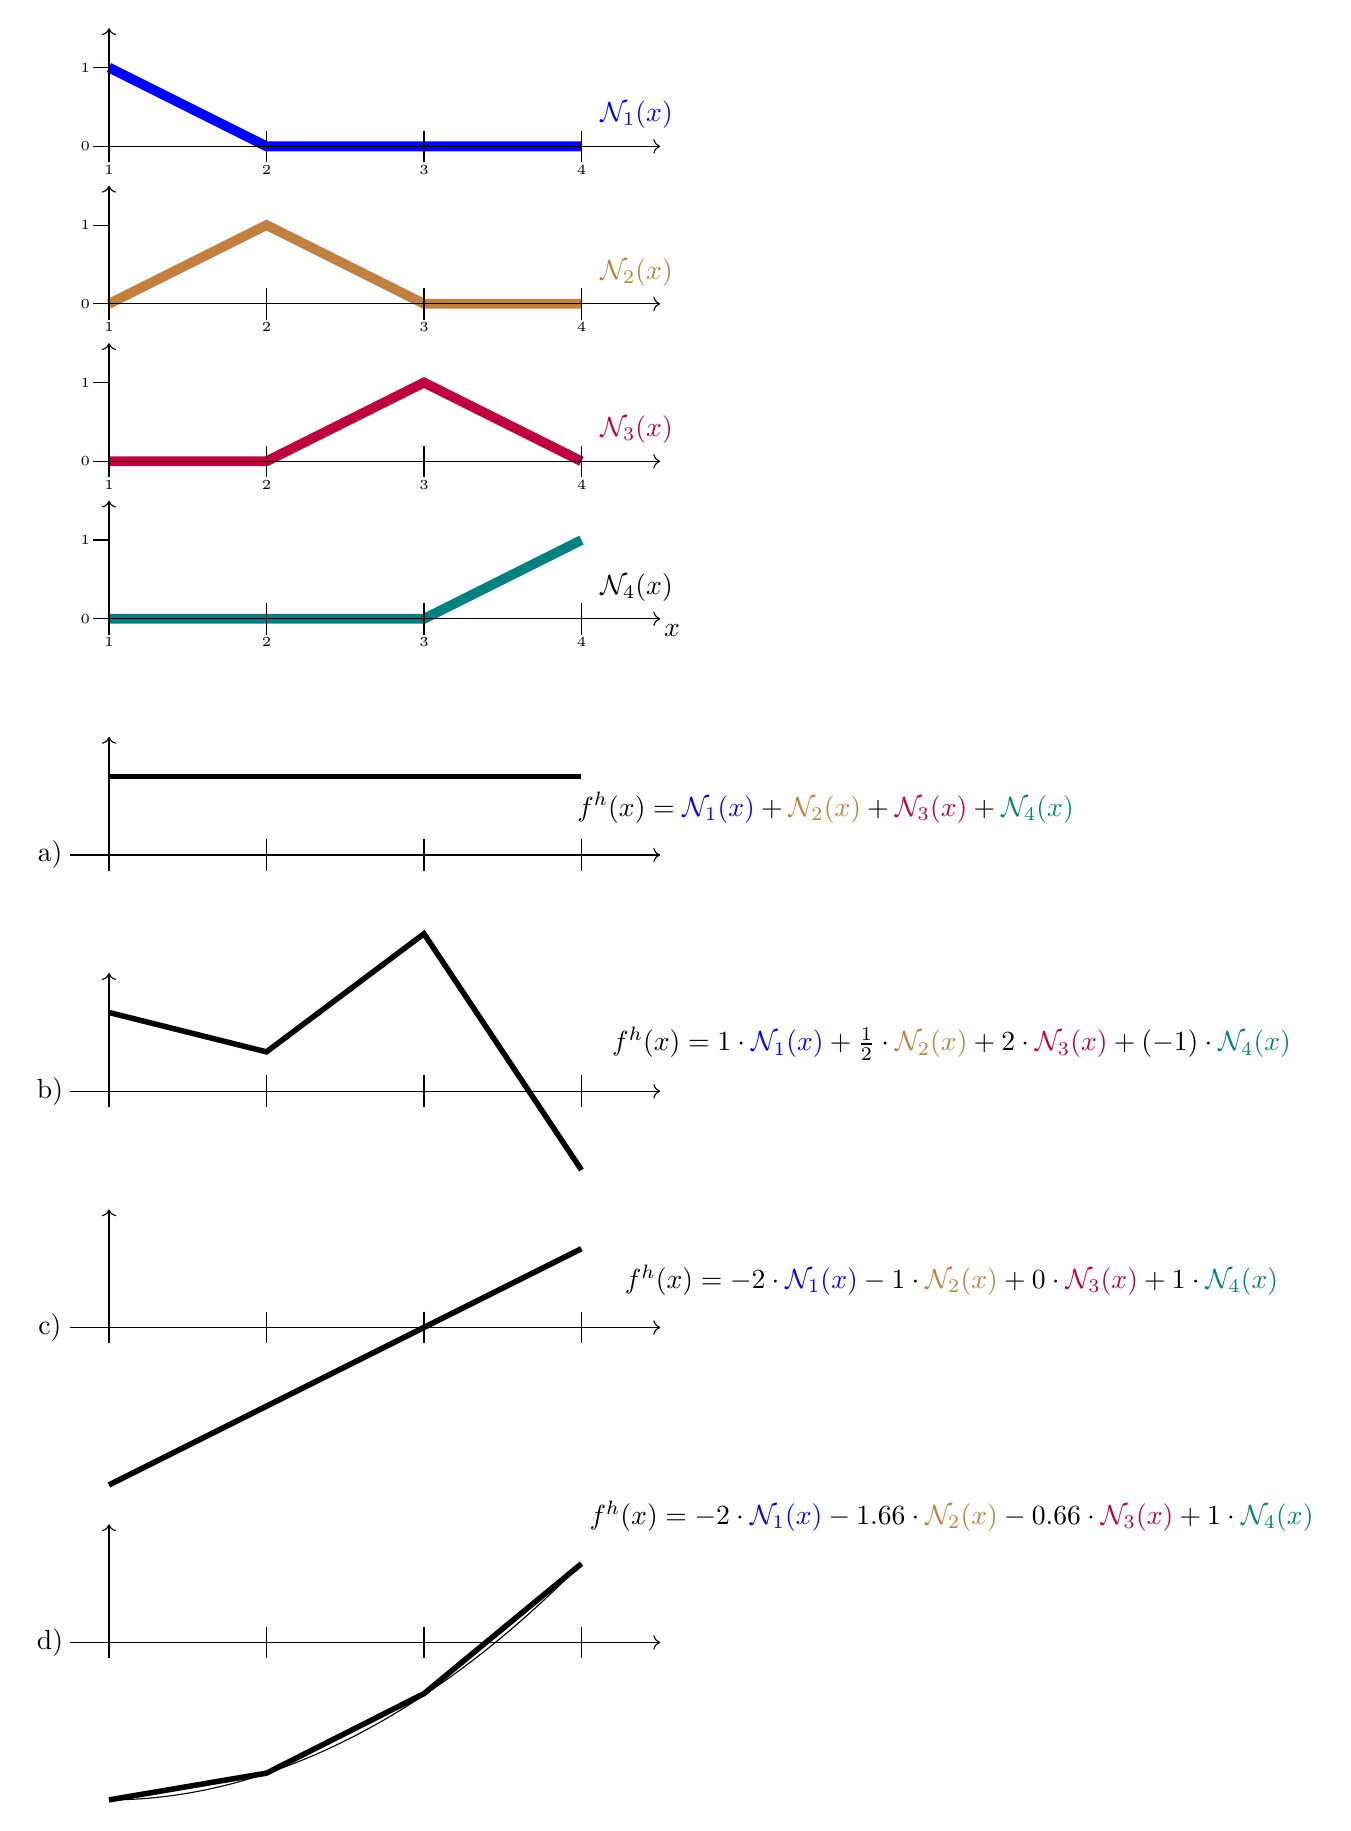
\begin{tikzpicture}
%\draw[step=0.5cm,gray,very thin] (0,-15) grid (15,10); 

%N1
\node[] at (7.7,7.4) {\color{blue}$\bN_1(x)$};
\draw[line width=1.25mm,color=blue] (1,8)--(3,7)--(5,7)--(7,7);
\draw [->] (0.8,7) -- (8,7);
\draw [->] (1,7) -- (1,8.5);
\draw [-] (1,6.8) -- (1,7.2);
\draw [-] (3,6.8) -- (3,7.2);
\draw [-] (5,6.8) -- (5,7.2);
\draw [-] (7,6.8) -- (7,7.2);

%N2
\node[] at (7.7,5.4) {\color{brown} $\bN_2(x)$};
\draw[line width=1.25mm,color=brown] (1,5)--(3,6)--(5,5)--(7,5);
\draw [->] (0.8,5) -- (8,5);
\draw [->] (1,5) -- (1,6.5);
\draw [-] (1,4.8) -- (1,5.2);
\draw [-] (3,4.8) -- (3,5.2);
\draw [-] (5,4.8) -- (5,5.2);
\draw [-] (7,4.8) -- (7,5.2);

%N3
\node[] at (7.7,3.4) {\color{purple}$\bN_3(x)$};
\draw[line width=1.25mm,color=purple] (1,3)--(3,3)--(5,4)--(7,3);
\draw [->] (0.8,3) -- (8,3);
\draw [->] (1,3) -- (1,4.5);
\draw [-] (1,2.8) -- (1,3.2);
\draw [-] (3,2.8) -- (3,3.2);
\draw [-] (5,2.8) -- (5,3.2);
\draw [-] (7,2.8) -- (7,3.2);

%N4
\node[] at (7.7,1.4) {$\bN_4(x)$};
\draw[line width=1.25mm,color=teal] (1,1)--(5,1)--(7,2);
\draw [->] (0.8,1) -- (8,1);
\draw [->] (1,1) -- (1,2.5);
\draw [-] (1,0.8) -- (1,1.2);
\draw [-] (3,0.8) -- (3,1.2);
\draw [-] (5,0.8) -- (5,1.2);
\draw [-] (7,0.8) -- (7,1.2);

\node[] at (8.15,0.85) {$x$};


\node[] at (1,6.7) {\tiny $1$};
\node[] at (3,6.7) {\tiny $2$};
\node[] at (5,6.7) {\tiny $3$};
\node[] at (7,6.7) {\tiny $4$};

\node[] at (1,4.7) {\tiny $1$};
\node[] at (3,4.7) {\tiny $2$};
\node[] at (5,4.7) {\tiny $3$};
\node[] at (7,4.7) {\tiny $4$};

\node[] at (1,2.7) {\tiny $1$};
\node[] at (3,2.7) {\tiny $2$};
\node[] at (5,2.7) {\tiny $3$};
\node[] at (7,2.7) {\tiny $4$};

\node[] at (1,0.7) {\tiny $1$};
\node[] at (3,0.7) {\tiny $2$};
\node[] at (5,0.7) {\tiny $3$};
\node[] at (7,0.7) {\tiny $4$};

\draw [-] (0.8,8) -- (1,8); \node[] at (0.7,7) {\tiny $0$}; \node[] at (0.7,8) {\tiny $1$};
\draw [-] (0.8,6) -- (1,6); \node[] at (0.7,5) {\tiny $0$}; \node[] at (0.7,6) {\tiny $1$};
\draw [-] (0.8,4) -- (1,4); \node[] at (0.7,3) {\tiny $0$}; \node[] at (0.7,4) {\tiny $1$};
\draw [-] (0.8,2) -- (1,2); \node[] at (0.7,1) {\tiny $0$}; \node[] at (0.7,2) {\tiny $1$};



\node[] at (0.25,-2) {a)};
\node[] at (10.1,-1.4) {$f^h(x)={\color{blue}\bN_1(x)}+{\color{brown} \bN_2(x)}
+{\color{purple}\bN_3(x)}+{\color{teal}\bN_4(x)}$};
\draw[line width=0.7mm] (1,-1)--(7,-1);
\draw [->] (0.5,-2) -- (8,-2);
\draw [->] (1,-2) -- (1,-0.5);
\draw [-] (1,-1.8) -- (1,-2.2);
\draw [-] (3,-1.8) -- (3,-2.2);
\draw [-] (5,-1.8) -- (5,-2.2);
\draw [-] (7,-1.8) -- (7,-2.2);

\node[] at (0.25,-5) {b)};
\node[] at (11.7,-4.4) {$f^h(x)=1\cdot {\color{blue}\bN_1(x)}+\frac12\cdot {\color{brown} \bN_2(x)}
+2\cdot {\color{purple}\bN_3(x)}+(-1)\cdot {\color{teal}\bN_4(x)}$};
\draw [->] (0.5,-5) -- (8,-5);
\draw [->] (1,-5) -- (1,-3.5);
\draw [-] (1,-4.8) -- (1,-5.2);
\draw [-] (3,-4.8) -- (3,-5.2);
\draw [-] (5,-4.8) -- (5,-5.2);
\draw [-] (7,-4.8) -- (7,-5.2);
\draw[line width=0.7mm] (1,-4)--(3,-4.5)--(5,-3)--(7,-6);

\node[] at (0.25,-8) {c)};
\node[] at (11.7,-7.4) {$f^h(x)=-2\cdot {\color{blue}\bN_1(x)}-1\cdot {\color{brown} \bN_2(x)}
+0\cdot {\color{purple}\bN_3(x)}+1\cdot {\color{teal}\bN_4(x)}$};
\draw [->] (0.5,-8) -- (8,-8);
\draw [->] (1,-8) -- (1,-6.5);
\draw [-] (1,-7.8) -- (1,-8.2);
\draw [-] (3,-7.8) -- (3,-8.2);
\draw [-] (5,-7.8) -- (5,-8.2);
\draw [-] (7,-7.8) -- (7,-8.2);
\draw[line width=0.7mm] (1,-10)--(3,-9)--(5,-8)--(7,-7);

\node[] at (0.25,-12) {d)};
\draw [->] (0.5,-12) -- (8,-12);
\draw [->] (1,-12) -- (1,-10.5);
\draw [-] (1,-11.8) -- (1,-12.2);
\draw [-] (3,-11.8) -- (3,-12.2);
\draw [-] (5,-11.8) -- (5,-12.2);
\draw [-] (7,-11.8) -- (7,-12.2);
\draw (1,-14) parabola (7,-11);
\draw[line width=0.7mm] (1,-14)--(3,-13.66)--(5,-12.65)--(7,-11);
\node[] at (11.7,-10.4) {$f^h(x)=-2\cdot {\color{blue}\bN_1(x)}-1.66\cdot {\color{brown} \bN_2(x)}
-0.66\cdot {\color{purple}\bN_3(x)}+1\cdot {\color{teal}\bN_4(x)}$};


\end{tikzpicture}
\end{center}





The four cases a,b,c,d are examples of combinations of these basis functions:
\[
f_h(x)=\sum_{i=1}^4 N_i(x) f_i
\]
Where $f_i$ are the values associated to the four nodes. 
We assume that the distance $h$ between nodes is 1.

Example a) illustrates the fact that the sum of all basis functions must be strictly equal to one everywhere
in the domain. Failing to do so would mean that the basis functions cannot represent a constant field (see
Section~\ref{ss:q12d}). 

Example b) illustrates a somewhat random combination of the basis functions, yielding a broken line. 

Example c) illustrates the fact that these linear basis functions can exactly represent a
linear function. When $f(x)=x-2$, then $f_1=f(0)=-2$, $f_2=f(1)=-1$, $f_3=f(2)=0$ and $f_4=f(3)=+1$, 
then $f_h(x)$ is exactly $f(x)$ on the domain.

Example d) illustrates the fact that linear basis functions cannot represent a parabola. Smaller and 
smaller elements will do an increasingly better job and will get closer to the curve but a 
systematic error will subsist.  


Note that these drawings are trivial to produce since $N_i(x_j)=\delta_{ij}$ by definition, so that 
$f_h(x_j)=f_j$.

%........................................................................
\subsubsection{In two dimensions}



 %-------------------
 %%%%%%%%%%%%%%%%%%%%%%%%%%%%%%%%%%%%%%%%%%%%%%%%%%%%%%%%%%%%%%%%%%%%%%%%%%%%

%%%%%%%%%%%%%%%%%%%%%%%%%%%%%%%%%%%%%%%%%%%%%%%%%%%%%%%%%%%%%%%%%%%%%%%%%%%%%%%%%%%%%%%%%%%%%%%%%%%
%\chapter{Solving the heat transport equation with linear Finite Elements \label{chapt5}} %%%%%%%%%
\include{chapter_fem1} %%%%%%%%%%%%%%%%%%%%%%%%%%%%%%%%%%%%%%%%%%%%%%%%%%%%%%%%%%%%%%%%%%%%%%%%%%%%

%%%%%%%%%%%%%%%%%%%%%%%%%%%%%%%%%%%%%%%%%%%%%%%%%%%%%%%%%%%%%%%%%%%%%%%%%%%%%%%%%%%%%%%%%%%%%%%%%%%
%\chapter{Solving the flow equations with the FEM} \label{solvingFEM} %%%%%%%%%%%%%%%%%%%%%%%%%%%%%
\chapter{Solving the flow equations with the FEM} \label{solvingFEM} %%%%%%%%%%%%%%%%%%%%%%%%%%%%%%

\begin{flushright} {\tiny {\color{gray} chapter6.tex}} \end{flushright}

%6.3 of donea and huerta

In the case of an incompressible flow, we have seen that the continuity (mass conservation)
equation takes the simple form ${\bm \nabla}\cdot{\bm v}=0$. In other word flow takes place 
under the constraint that the divergence of its velocity field is exactly zero eveywhere 
(solenoidal constraint), i.e. it is divergence free. \index{divergence free}

We see that the pressure in the momentum equation is then a degree of freedom which is needed 
to satisfy the incompressibilty constraint (and it is not related to any constitutive equation)
\cite{dohu}. In other words the pressure is acting as a Lagrange multiplier of the incompressibility
constraint. 

Various approaches have been proposed in the literature to deal with the 
incompressibility constraint but we will only focus on the penalty method 
(section \ref{sec_penalty}) and the so-called mixed finite element method
\ref{sec_mixed}.
 %---------------------------------------------------------------------------
\section{Strong and weak forms} \begin{flushright} {\tiny {\color{gray} \tt strongweak.tex}} \end{flushright}
%------------------------------------------------------------------------------

\index{general}{strong form} 

As we have seen in Section~\ref{sec:diff1D}
the strong form consists of the governing equation and the boundary conditions, i.e. 
the mass, momentum and energy conservation equations supplemented with Dirichlet and/or Neumann
boundary conditions on (parts of) the boundary. Ultimately we have two main unknowns that 
we wish to solve for: velocity (a vector) and pressure (a scalar).

\index{general}{weak form}
To develop the finite element formulation, the partial differential equations 
must be restated in an integral form called the weak form. In essence the PDEs are 
first multiplied by an arbitrary function and integrated over the domain.

 %--------------------------------------------
\section{Which velocity-pressure pair for Stokes?}\label{ss:pair}\subsubsection{The bi/tri-linear velocity - constant pressure element ($Q_1\times P_0$)}
\includegraphics[width=3cm]{images/under_construction}

\subsubsection{The bi/tri-quadratic velocity - discontinuous linear pressure element ($Q_2 \times P_{-1}$)}
\includegraphics[width=3cm]{images/under_construction}

\subsubsection{The bi/tri-quadratic velocity - bi/tri-linear pressure element ($Q_2 \times Q_1$)}
\includegraphics[width=3cm]{images/under_construction}

\subsubsection{The stabilised bi/tri-linear velocity -  bi/tri-linear pressure element ($Q_1\times Q_1$-stab)}
\includegraphics[width=3cm]{images/under_construction}

\subsubsection{The MINI triangular element ($P_1^+\times P_1$)}
\includegraphics[width=3cm]{images/under_construction}

\subsubsection{The quadratic velocity - linear pressure triangle ($P_2\times P_1$)}
\includegraphics[width=3cm]{images/under_construction}

\subsubsection{The Crouzeix-Raviart triangle ($P_2^+\times P_{-1}$)}
\includegraphics[width=3cm]{images/under_construction}

\subsection{Other elements}

P1P0

P1P1

Q2Q2

P2P2

 %-----------------

\newpage
\section{The penalty approach for viscous flow}\label{sec:penalty}\begin{flushright} {\tiny {\color{gray} penalty.tex}} \end{flushright}
%~~~~~~~~~~~~~~~~~~~~~~~~~~~~~~~~~~~~~~~~~~~~~~~~~~~~~~~~~~~~~~~~~~~~~~~~~~~~~~~~~~~~~~~~~~~~~~~~~~

\label{sec_penalty}

\index{general}{Penalty Formulation}

In order to impose the incompressibility constraint, two widely used procedures are available, namely the 
Lagrange multiplier method and the penalty method \cite{bathe82,hugh}. The latter is implemented in {\sc elefant}, which allows for the elimination of the pressure variable from the momentum equation (resulting in a reduction of the matrix size).%, based on a relaxation of the incompressibility constraint. 

Mathematical details on the origin and validity of the penalty approach applied to the Stokes problem can for instance be found in  \cite{cuss86}, \cite{redd82} or \cite{gunz89}.

The penalty formulation of the mass conservation equation is based on a relaxation of the incompressibility constraint and writes 
\begin{equation}
{\vec \nabla}\cdot {\vec \upnu} + \frac{p}{\lambda} = 0 \label{penal}
\end{equation}
where $\lambda$ is the penalty parameter, that can be interpreted (and has the same dimension) as a bulk viscosity. It is 
equivalent to say that the material is weakly compressible. It can be shown that if one chooses $\lambda$ to be a 
sufficiently large number, the continuity equation $ {\vec \nabla}\cdot {\vec \upnu} = 0$ will be approximately satisfied in the finite element solution. The value of $\lambda$ is often recommended to be 6 to 7 orders of magnitude larger than the shear viscosity \cite{dohu03,hulb79}.

%Note that Eq. (\ref{penal}) does not form the basis of the penalty method (as often implied) for the Stokes equation but is a consequence of minimising a modified functional of the problem under certain assumptions \cite{redd82}. 

Equation (\ref{penal}) can be used to eliminate the pressure in the momentum equation 
so that the mass and momentum conservation equations fuse to become :
\begin{equation}
{\vec \nabla}\cdot ( 2 \eta \dot\varepsilon({\vec \upnu})) 
+ \lambda {\vec \nabla} ({\vec \nabla }\cdot {\vec \upnu}) = \rho {\bm g} = 0 \label{peneq}
\end{equation}

\cite{mahu78} have established the equivalence for incompressible problems between the reduced integration
of the penalty term and a mixed Finite Element approach if the pressure nodes coincide with the integration points of the reduced rule.

In the end, the elimination of the pressure unknown in the Stokes equations
replaces the original saddle-point Stokes problem \cite{begl05} by an elliptical problem, 
which leads to a symmetric positive definite (SPD) FEM matrix. 
%Such systems always admit a square root triangular matrix (the Cholesky factor, L) and can be solved, once L has been computed (Cholesky factorization), by 2 triangular matrix solves (upper and lower back-substitutions). 
This is the major benefit of the penalized approach 
over the full indefinite solver with the velocity-pressure variables. Indeed, the SPD character of the matrix lends itself 
to efficient solving stragegies and is less memory-demanding since it is sufficient to store only the upper half of the matrix including the diagonal
\cite{gova}
.
\improvement{list codes which use this approach}

%The stress tensor ${\bm \sigma}$ is symmetric ({\it i.e.} $\sigma_{ij}=\sigma_{ji}$). For simplicity
%I will now focus on a Stokes flow in two dimensions. 

Since the penalty formulation is only valid for incompressible flows, then 
$\dot{\bm \epsilon}=\dot{\bm \epsilon}^d$ so that the $d$ superscript is ommitted in what follows.
Because the stress tensor is symmetric one can also rewrite it the following vector format:
\begin{eqnarray}
\left(
\begin{array}{c}
\sigma_{xx}\\
\sigma_{yy}\\
\sigma_{zz}\\
\sigma_{xy}\\
\sigma_{xz}\\
\sigma_{yz}
\end{array}
\right)
&=&
\left(
\begin{array}{c}
-p\\
-p\\
-p\\
0\\
0\\
0
\end{array}
\right)
+2 \eta
\left(
\begin{array}{c}
\dot{\epsilon}_{xx}\\
\dot{\epsilon}_{yy}\\
\dot{\epsilon}_{zz}\\
\dot{\epsilon}_{xy}\\
\dot{\epsilon}_{xz}\\
\dot{\epsilon}_{yz}
\end{array}
\right)
\nonumber\\
&=&
\lambda
\left(
\begin{array}{c}
\dot{\epsilon}_{xx} + \dot{\epsilon}_{yy} + \dot{\epsilon}_{zz}\\
\dot{\epsilon}_{xx} + \dot{\epsilon}_{yy} + \dot{\epsilon}_{zz}\\
\dot{\epsilon}_{xx} + \dot{\epsilon}_{yy} + \dot{\epsilon}_{zz}\\
0 \\ 0 \\ 0
\end{array}
\right)
+2 \eta
\left(
\begin{array}{c}
\dot{\epsilon}_{xx}\\
\dot{\epsilon}_{yy}\\
\dot{\epsilon}_{zz}\\
\dot{\epsilon}_{xy}\\
\dot{\epsilon}_{xz}\\
\dot{\epsilon}_{yz}
\end{array}
\right)\nonumber\\
&=&
\left[
\lambda
\underbrace{
\left(
\begin{array}{cccccc}
1 & 1 & 1 & 0 & 0 & 0 \\
1 & 1 & 1 & 0 & 0 & 0 \\
1 & 1 & 1 & 0 & 0 & 0 \\
0 & 0 & 0 & 0 & 0 & 0 \\
0 & 0 & 0 & 0 & 0 & 0 \\
0 & 0 & 0 & 0 & 0 & 0 
\end{array}
\right)}_{\bm K}
+ \eta
\underbrace{
\left(
\begin{array}{cccccc}
2 & 0 & 0 & 0 & 0 & 0 \\ 
0 & 2 & 0 & 0 & 0 & 0 \\ 
0 & 0 & 2 & 0 & 0 & 0 \\ 
0 & 0 & 0 & 1 & 0 & 0 \\
0 & 0 & 0 & 0 & 1 & 0 \\
0 & 0 & 0 & 0 & 0 & 1 
\end{array}
\right)
}_{\bm C}
\right]
\cdot
\left(
\begin{array}{c}
\frac{\partial u}{\partial x} \\ \\
\frac{\partial v}{\partial y} \\ \\
\frac{\partial w}{\partial z} \\ \\
\frac{\partial u}{\partial y} + \frac{\partial v}{\partial x} \\ \\
\frac{\partial u}{\partial z} + \frac{\partial w}{\partial x} \\ \\
\frac{\partial v}{\partial z} + \frac{\partial w}{\partial y} 
\end{array}
\right) \nonumber
\end{eqnarray}


Remember that
\[
\frac{\partial u}{\partial x} = \sum_{i=1}^4 \frac{\partial \bN_i}{\partial x}\;  u_i 
\quad\quad
\frac{\partial v}{\partial y} = \sum_{i=1}^4 \frac{\partial \bN_i}{\partial y}\;  v_i 
\quad\quad
\frac{\partial w}{\partial z} = \sum_{i=1}^4 \frac{\partial \bN_i}{\partial z}\;  w_i 
\]
and 
\begin{eqnarray}
\frac{\partial u}{\partial y} +\frac{\partial v}{\partial x} 
&=& \sum_{i=1}^4 \frac{\partial \bN_i}{\partial y}\;  u_i
+ \sum_{i=1}^4 \frac{\partial \bN_i}{\partial x}\;  v_i \nonumber\\
\frac{\partial u}{\partial z} +\frac{\partial w}{\partial x} 
&=& \sum_{i=1}^4 \frac{\partial \bN_i}{\partial z}\;  u_i
+ \sum_{i=1}^4 \frac{\partial \bN_i}{\partial x}\;  w_i \nonumber\\
\frac{\partial v}{\partial z} +\frac{\partial w}{\partial y} 
&=& \sum_{i=1}^4 \frac{\partial \bN_i}{\partial z}\;  v_i
+ \sum_{i=1}^4 \frac{\partial \bN_i}{\partial y}\;  w_i \nonumber
\end{eqnarray}
so that
\[
\left(
\begin{array}{c}
\frac{\partial u}{\partial x} \\ \\
\frac{\partial v}{\partial y} \\ \\
\frac{\partial w}{\partial z} \\ \\
\frac{\partial u}{\partial y} + \frac{\partial v}{\partial x} \\ \\
\frac{\partial u}{\partial z} + \frac{\partial w}{\partial x} \\ \\
\frac{\partial v}{\partial z} + \frac{\partial w}{\partial y} 
\end{array}
\right)
=
\underbrace{
\left(
\begin{array}{ccccccccccccc}
\frac{\partial \bN_1}{\partial x} & 0 & 0 &  
\frac{\partial \bN_2}{\partial x} & 0 & 0 &
\frac{\partial \bN_3}{\partial x} & 0 & 0 & \dots &
\frac{\partial \bN_4}{\partial x} & 0 & 0 \\  \\
0 & \frac{\partial \bN_1}{\partial y} & 0 &
0 & \frac{\partial \bN_2}{\partial y} & 0 &
0 & \frac{\partial \bN_3}{\partial y} & 0 & \dots &
0 & \frac{\partial \bN_4}{\partial y} & 0  \\ \\
0 & 0 & \frac{\partial \bN_1}{\partial z}  &
0 & 0 & \frac{\partial \bN_2}{\partial z}  &
0 & 0 & \frac{\partial \bN_3}{\partial z}  & \dots &
0 & 0 & \frac{\partial \bN_4}{\partial z}   \\ \\
\frac{\partial \bN_1}{\partial y} &  \frac{\partial \bN_1}{\partial x} & 0 &
\frac{\partial \bN_2}{\partial y} &  \frac{\partial \bN_2}{\partial x} & 0 &
\frac{\partial \bN_3}{\partial y} &  \frac{\partial \bN_3}{\partial x} & 0 & \dots &
\frac{\partial \bN_4}{\partial y} &  \frac{\partial \bN_4}{\partial x} & 0 \\ \\ 
\frac{\partial \bN_1}{\partial z} & 0 &\frac{\partial \bN_1}{\partial x}  &
\frac{\partial \bN_2}{\partial z} & 0 &\frac{\partial \bN_2}{\partial x}  &
\frac{\partial \bN_3}{\partial z} & 0 &\frac{\partial \bN_3}{\partial x}  & \dots &
\frac{\partial \bN_4}{\partial z} & 0 &\frac{\partial \bN_4}{\partial x}  \\ \\ 
0 & \frac{\partial \bN_1}{\partial z} &  \frac{\partial \bN_1}{\partial y}  &
0 & \frac{\partial \bN_2}{\partial z} &  \frac{\partial \bN_2}{\partial y}  &
0 & \frac{\partial \bN_3}{\partial z} &  \frac{\partial \bN_3}{\partial y}  & \dots &
0 & \frac{\partial \bN_4}{\partial z} &  \frac{\partial \bN_4}{\partial y} 
\end{array}
\right)
}_{\bm B (6\times 24) }
\cdot
\underbrace{
\left(
\begin{array}{c}
u1 \\ v1 \\ w1 \\ u2 \\ v2 \\ w2 \\ u3 \\ v3 \\ w3 \\ \dots \\ u8 \\ v8 \\ w8
\end{array}
\right)
}_{\vec V (24\times1)}
\]
Finally,
\[
\vec{\sigma}=
\left(
\begin{array}{c}
\sigma_{xx}\\
\sigma_{yy}\\
\sigma_{zz}\\
\sigma_{xy}\\
\sigma_{xz}\\
\sigma_{yz}
\end{array}
\right)
=
(\lambda {\bm K} +  \eta {\bm C} )\cdot {\bm B} \cdot {\vec V}
\]
We will now establish the weak form of the momentum conservation equation. 
\index{general}{Weak Form}
We start again from 
\[
{\vec \nabla}\cdot {\bm \sigma} + {\vec b} = {\vec 0} 
\]
For the $\bN_i$'s 'regular enough', we can write:
\[
\int_{\Omega_e} \bN_i {\vec \nabla}\cdot {\bm \sigma} d\Omega + \int_{\Omega_e} \bN_i  {\vec b} \;  d\Omega =0
\]
We can integrate by parts and drop the surface term\footnote{We will come back to this at a later stage}:
\[
\int_{\Omega_e} {\vec \nabla } \bN_i \cdot {\bm \sigma} \; d\Omega = \int_{\Omega_e} \bN_i  {\vec b}\;  d\Omega 
\]
or, 
\[
\int_{\Omega_e} 
\left(
\begin{array}{cccccc}
\frac{\partial \bN_i}{\partial x} & 0 & 0 & 
\frac{\partial \bN_i}{\partial y} & 
\frac{\partial \bN_i}{\partial z} & 0 \\  \\
0 & \frac{\partial \bN_i}{\partial y} &  0 & 
\frac{\partial \bN_i}{\partial x}  & 0 & \frac{\partial \bN_i}{\partial z} \\ \\
0 & 0 & \frac{\partial \bN_i}{\partial z} & 0 & 
\frac{\partial \bN_i}{\partial x} &  \frac{\partial \bN_i}{\partial y} 
\end{array}
\right)
\cdot
\left(
\begin{array}{c}
\sigma_{xx}\\
\sigma_{yy}\\
\sigma_{zz}\\
\sigma_{xy}\\
\sigma_{xz}\\
\sigma_{yz}
\end{array}
\right) \;
d\Omega = \int_{\Omega_e} \bN_i {\vec b} \;  d\Omega 
\]
Let $i=1,2,3,4,\dots 8$ and stack the resulting eight equations on top of one another. 
\begin{eqnarray}
\int_{\Omega_e} 
\left(
\begin{array}{cccccc}
\frac{\partial \bN_i}{\partial x} & 0 & 0 & 
\frac{\partial \bN_i}{\partial y} & 
\frac{\partial \bN_i}{\partial z} & 0 \\  \\
0 & \frac{\partial \bN_i}{\partial y} &  0 & 
\frac{\partial \bN_i}{\partial x}  & 0 & \frac{\partial \bN_i}{\partial z} \\ \\
0 & 0 & \frac{\partial \bN_i}{\partial z} & 0 & 
\frac{\partial \bN_i}{\partial x} &  \frac{\partial \bN_i}{\partial y} 
\end{array}
\right)
\cdot
\left(
\begin{array}{c}
\sigma_{xx}\\
\sigma_{yy}\\
\sigma_{zz}\\
\sigma_{xy}\\
\sigma_{xz}\\
\sigma_{yz}
\end{array}
\right)
d\Omega &=& \int_{\Omega_e} \bN_1 
\left(
\begin{array}{c}
b_x \\ b_y \\ b_z
\end{array}
\right)
 d\Omega \nonumber\\
\int_{\Omega_e} 
\left(
\begin{array}{cccccc}
\frac{\partial \bN_i}{\partial x} & 0 & 0 & 
\frac{\partial \bN_i}{\partial y} & 
\frac{\partial \bN_i}{\partial z} & 0 \\  \\
0 & \frac{\partial \bN_i}{\partial y} &  0 & 
\frac{\partial \bN_i}{\partial x}  & 0 & \frac{\partial \bN_i}{\partial z} \\ \\
0 & 0 & \frac{\partial \bN_i}{\partial z} & 0 & 
\frac{\partial \bN_i}{\partial x} &  \frac{\partial \bN_i}{\partial y} 
\end{array}
\right)
\cdot
\left(
\begin{array}{c}
\sigma_{xx}\\
\sigma_{yy}\\
\sigma_{zz}\\
\sigma_{xy}\\
\sigma_{xz}\\
\sigma_{yz}
\end{array}
\right)
d\Omega &=& \int_{\Omega_e} \bN_2 
\left(
\begin{array}{c}
b_x \\ b_y \\ b_z
\end{array}
\right) \;
d\Omega \nonumber\\ \nonumber\\
&\dots& \nonumber\\ \nonumber\\
\int_{\Omega_e} 
\left(
\begin{array}{cccccc}
\frac{\partial \bN_8}{\partial x} & 0 & 0 & 
\frac{\partial \bN_8}{\partial y} & 
\frac{\partial \bN_8}{\partial z} & 0 \\  \\
0 & \frac{\partial \bN_8}{\partial y} &  0 & 
\frac{\partial \bN_8}{\partial x}  & 0 & \frac{\partial \bN_8}{\partial z} \\ \\
0 & 0 & \frac{\partial \bN_8}{\partial z} & 0 & 
\frac{\partial \bN_8}{\partial x} &  \frac{\partial \bN_8}{\partial y} 
\end{array}
\right)
\cdot
\left(
\begin{array}{c}
\sigma_{xx}\\
\sigma_{yy}\\
\sigma_{zz}\\
\sigma_{xy}\\
\sigma_{xz}\\
\sigma_{yz}
\end{array}
\right)
d\Omega &=& \int_{\Omega_e} \bN_8 
\left(
\begin{array}{c}
b_x \\ b_y \\ b_z
\end{array}
\right)
d\Omega 
\end{eqnarray}
We easily recognize ${\bm B}^T$ inside the integrals!
Let us define 
\[
{\vec \bN}_b^T=(\bN_1 b_x , \bN_1 b_y, \bN_1 b_z ... \bN_8 b_x, \bN_8 b_y, \bN_8 b_z)
\]
then we can write
\[
\int_{\Omega_e} {\bm B}^T \cdot 
\left(
\begin{array}{c}
\sigma_{xx}\\
\sigma_{yy}\\
\sigma_{zz}\\
\sigma_{xy}\\
\sigma_{xz}\\
\sigma_{yz}
\end{array}
\right)
d\Omega
=
\int_{\Omega_e} {\vec \bN}_b d\Omega 
\]
and finally:
\[
\int_{\Omega_e} {\bm B}^T \cdot [ \lambda {\bm K} + \eta {\bm C} ] \cdot {\bm B} \cdot {\vec V} d\Omega
=
\int_{\Omega_e} {\vec \bN}_b d\Omega 
\]
Since $\vec V$ contains is the vector of unknowns (i.e. the velocities at the corners), 
it does not depend on the $x$ or $y$ coordinates
so it can be taking outside of the integral:
\[
\underbrace{
\left(\int_{\Omega_e} {\bm B}^T \cdot [ \lambda {\bm K} + \eta {\bm C} ] \cdot {\bm B} \;  d\Omega \right) 
}_{\bm A_{el}(24 \times 24)}
\cdot 
\underbrace{
{\vec V}
}_{(24\times 1)}
=
\underbrace{
\int_{\Omega_e} {\vec \bN}_b d\Omega 
}_{\vec B_{el} (24\times 1)}
\]
or, 
\[
\left[
\underbrace{
\left(\int_{\Omega_e} \lambda {\bm B}^T \cdot {\bm K} \cdot {\bm B} \; d\Omega \right) 
}_{\bm A_{el}^\lambda(24 \times 24)}
+
\underbrace{
\left(\int_{\Omega_e}  \eta {\bm B}^T \cdot {\bm C}  \cdot {\bm B} \;  d\Omega \right) 
}_{\bm A_{el}^\eta(24 \times 24)}
\right]
\cdot 
\underbrace{
{\vec V}
}_{(24\times 1)}
=
\underbrace{
\int_{\Omega_e} {\vec \bN}_b d\Omega 
}_{\vec B_{el} (24\times 1)}
\]

\Literature \cite{odks82,dhhu86}

\todo[inline]{reduced integration \cite{hulb79} }

\todo[inline]{write about 3D to 2D}
 %-------------
\newpage
\section{The mixed FEM for viscous flow} \label{sec:mixed} \label{sec_mixed}

What follows is formulated in 2D as the extension to 3D is 
rather trivial. Also the flow is assumed to be incompressible, 
isoviscous, isothermal. 

The methodology to derive the discretised equations of the mixed system is 
quite similar to the one we have used in the case of the penalty formulation.
The big difference comes from the fact that we are now solving for both 
velocity and pressure at the same time, and that we therefore must solve 
the mass and momentum conservation equations together.
As before, velocity inside an element is given by 
\begin{equation}
{\vec \upnu}({\vec r})=\sum_{i=1}^{m_v} N_i^\upnu({\vec r})\;  {\vec \upnu}_i
\label{mixed01}
\end{equation}
where $N_i^{v}$ are the polynomial basis functions for the velocity,
and the summation runs over the $m_v$ nodes composing the element.
A similar expression is used for pressure:
\begin{equation}
p({\vec r})=\sum_{i=1}^{m_p} N_i^p({\vec r}) \; p_i
\label{mixed02}
\end{equation}
Note that the velocity is a vector of size while pressure (and temperature)
is a scalar. There are then $ndof_v$ velocity degrees of freedom per node
and $ndof_p$ pressure degrees of freedom.
It is also very important to remember that the numbers of 
velocity nodes and pressure nodes for a given element 
are more often than not different and that velocity and pressure
nodes need not be colocated. Indeed, unless 
co-called 'stabilised elements' are used, we have $m_v>m_p$, which 
means that the polynomial order of the velocity field is higher than 
the polynomial order of the pressure field (usually by value 1).

\todo[inline]{insert here link(s) to manual and literature} 

Other notations are sometimes used for Eqs.(\ref{mixed01},\ref{mixed02}):
\begin{equation}
u({\vec r}) = \vec{N}^\upnu \cdot \vec{u}
\quad\quad\quad\quad
v({\vec r}) = \vec{N}^\upnu \cdot \vec{v}
\quad\quad\quad\quad
p({\vec r}) = \vec{N}^p \cdot \vec{p}
\end{equation} 
where ${\vec \upnu}=(u,v)$ and $\vec{N}^\upnu$ is the vector containing all basis functions evaluated at location ${\vec r}$:
\begin{eqnarray}
\vec{N}^v &=& \left( N_1^\upnu({\vec r}),  N_2^\upnu({\vec r}),  N_3^\upnu({\vec r}), \dots  N_{m_v}^\upnu({\vec r}) \right) \\
\vec{N}^p &=& \left( N_1^p({\vec r}),  N_2^p({\vec r}),  N_3^p({\vec r}), \dots  N_{m_p}^p({\vec r}) \right)
\end{eqnarray}
and with 
\begin{eqnarray}
\vec{u} &=& \left( u_1,  u_2,  u_3, \dots  u_{m_v} \right) \\
\vec{v} &=& \left( v_1,  v_2,  v_3, \dots  v_{m_v} \right) \\
\vec{p} &=& \left( p_1,  p_2,  p_3, \dots  p_{m_p} \right) 
\end{eqnarray}
We will now establish the weak form of the momentum conservation equation. 
We start again from 
\begin{eqnarray}
{\vec \nabla}\cdot {\bm \sigma} + {\vec b} &=& {\vec 0} \\
{\vec \nabla}\cdot {\vec v} &=& 0
\end{eqnarray}
For the $N_i^\upnu$'s and $N_i^p$ 'regular enough', we can write:
\begin{eqnarray}
\int_{\Omega_e} N_i^\upnu {\vec \nabla}\cdot {\bm \sigma} d\Omega + \int_{\Omega_e} N_i^\upnu  {\vec b} \; d\Omega 
&=& \vec 0 \\
\int_{\Omega_e} N_i^p {\vec \nabla}\cdot {\vec v} d\Omega &=& 0
\end{eqnarray}
We can integrate by parts and drop the surface term\footnote{We will come back to this at a later stage}:
\begin{eqnarray}
\int_{\Omega_e} {\vec \nabla } N_i^\upnu \cdot {\bm \sigma} d\Omega &=& \int_{\Omega_e} N_i^\upnu  {\vec b} d\Omega \\
\int_{\Omega_e} N_i^p {\vec \nabla}\cdot {\vec v} d\Omega &=& 0
\end{eqnarray}
or, 
\begin{equation}
\int_{\Omega_e} 
\left(
\begin{array}{ccc}
\frac{\partial N_i^\upnu}{\partial x} & 0 & \frac{\partial N_i^\upnu}{\partial y} \\  \\
0 & \frac{\partial N_i^\upnu}{\partial y} &  \frac{\partial N_i^\upnu}{\partial x}  
\end{array}
\right)
\cdot
\left(
\begin{array}{c}
\sigma_{xx}\\
\sigma_{yy}\\
\sigma_{xy}\\
\end{array}
\right)
d\Omega = \int_{\Omega_e} N_i^\upnu {\vec b} d\Omega 
\end{equation}
As before (see section XXX) the above equation can ultimately be written:
\begin{equation}
\int_{\Omega_e} {\bm B}^T \cdot 
\left(
\begin{array}{c}
\sigma_{xx}\\
\sigma_{yy}\\
\sigma_{xy}\\
\end{array}
\right)
d\Omega
=
\int_{\Omega_e} {\vec N}_b d\Omega 
\end{equation}
We have previously established that the strain rate 
vector $\vec{\dot \varepsilon}$ is:
\begin{equation}
\vec{\dot\varepsilon}=
\left(
\begin{array}{c}
\frac{\partial u}{\partial x} \\ \\
\frac{\partial v}{\partial y} \\ \\
\frac{\partial u}{\partial y} + \frac{\partial v}{\partial x} \\
\end{array}
\right)
=
\underbrace{
\left(
\begin{array}{ccccccccccc}
\frac{\partial N_1^\upnu}{\partial x} & 0 & 
\frac{\partial N_2^\upnu}{\partial x} & 0 & 
\frac{\partial N_3^\upnu}{\partial x} & 0 & \dots & 
\frac{\partial N_{m_v}^\upnu}{\partial x} & 0
\\  \\
0 & \frac{\partial N_1^\upnu}{\partial y} & 
0 & \frac{\partial N_2^\upnu}{\partial y} &
0 & \frac{\partial N_3^\upnu}{\partial y} & \dots & 
0 & \frac{\partial N_{m_v}^\upnu}{\partial x} 
\\ \\
\frac{\partial N_1^\upnu}{\partial y} &  \frac{\partial N_1^\upnu}{\partial x} &  
\frac{\partial N_2^\upnu}{\partial y} &  \frac{\partial N_2^\upnu}{\partial x} & 
\frac{\partial N_3^\upnu}{\partial y} &  \frac{\partial N_3^\upnu}{\partial x} &   \dots &  
\frac{\partial N_{m_v}^\upnu}{\partial y} &  \frac{\partial N_{m_v}^\upnu}{\partial x}  
\end{array}
\right) 
}_{\bm B}
\cdot
\underbrace{
\left(
\begin{array}{c}
u_1 \\ v_1 \\ u_2 \\ v_2 \\ u_3 \\ v_3 \\ \dots \\ u_{m_v} \\ v_{m_v}
\end{array}
\right)
}_{\vec V}
\end{equation}
or, $\vec{\dot \varepsilon}={\bm B}\cdot {\vec V}$ where ${\bm B}$ is the gradient 
matrix and ${\vec V}$ is the vector of all vector degrees of freedom for the 
element. The matrix ${\bm B}$ is then of size $3\times m_v$ and the vector
${\vec V}$ is $m_v$ long.
we have 
\begin{eqnarray}
\sigma_{xx}&=&-p + 2\eta \dot\varepsilon_{xx} \\
\sigma_{yy}&=&-p + 2\eta \dot\varepsilon_{yy} \\
\sigma_{xy}&=& \hspace{5.5mm} + 2\eta \dot\varepsilon_{xy} 
\end{eqnarray}
so
\begin{equation}
\vec{\sigma} 
=-\left( 
\begin{array}{c}
1 \\ 1 \\ 0 
\end{array}
\right) p+ {\bm C} \cdot \vec{\dot\varepsilon}
=
- \left(
\begin{array}{c}
1 \\ 1 \\ 0 
\end{array}
\right)
\vec{N^p} \cdot {\vec P}  + 
{\bm C} \cdot  {\bm B}\cdot {\vec V}
\end{equation}
with
\begin{equation}
{\bm C}=
\left(
\begin{array}{ccc}
2 & 0 & 0 \\
0 & 2 & 0 \\
0 & 0 & 1  
\end{array}
\right)
\quad\quad\quad
\vec{\dot \varepsilon} = 
\left(
\begin{array}{c}
\dot \varepsilon_{xx} \\
\dot \varepsilon_{yy} \\
2\dot \varepsilon_{xy} 
\end{array}
\right)
\end{equation}
Let us define matrix ${\bm N}^p$ of size $3\times m_p$:
\begin{equation}
{\bm N}^p=
\left(
\begin{array}{c}
1 \\ 1 \\ 0
\end{array}
\right)
\vec{N^p} 
=
\left(
\begin{array}{c}
\vec{N^p} \\
\vec{N^p} \\
0
\end{array}
\right)
\end{equation}
so that
\begin{equation}
\vec{\sigma} 
= - {\bm N}^p
 \cdot {\vec P}  + 
{\bm C} \cdot  {\bm B}\cdot {\vec V}
\end{equation}
finally
\begin{equation}
\int_{\Omega_e} {\bm B}^T \cdot 
[
- {\bm N}^p  \cdot {\vec P}  + {\bm C} \cdot  {\bm B}\cdot {\vec V}
]
d\Omega
=
\int_{\Omega_e} {\bm N}_b d\Omega 
\end{equation}
or,
\begin{equation}
\underbrace{\left(-\int_{\Omega_e} {\bm B}^T \cdot 
{\bm N}^p  
d\Omega \right)}_{\G} \cdot {\vec P} 
+
\underbrace{
\left(
\int_{\Omega_e} {\bm B}^T \cdot 
{\bm C} \cdot  {\bm B}
d\Omega
\right)}_{\K}
\cdot {\vec V}
=
\underbrace{\int_{\Omega_e} {\vec N}_b d\Omega }_{\vec f}
\end{equation}
where the matrix $\K$ is of size $(m_v*ndof_v \times m_v*ndof_v)$, 
and matrix ${\G}$ is of size $(m_v*ndof_v \times m_p*ndof_p)$.
Turning now to the mass conservation equation:
\begin{eqnarray}
0&=&\int_{\Omega_e} \vec{N}^p {\vec \nabla}\cdot {\vec v} \; d\Omega \nonumber\\
&=& \int_{\Omega_e} \vec{N}^p \sum_{i=1}^{m_v} 
\left( \frac{\partial N_i^\upnu}{\partial x} u_i + \frac{\partial N_i^\upnu}{\partial y} v_i \right)  
d\Omega \nonumber\\
&=& 
\int_{\Omega_e} 
\left(
\begin{array}{c}
N_1^p \left(\sum\limits_{i=1}^{m_v} \frac{\partial N_i^\upnu }{\partial x} u_i +
\sum\limits_{i=1}^{m_v} \frac{\partial N_i^\upnu }{\partial x} v_i \right) \\
N_2^p \left(\sum\limits_{i=1}^{m_v} \frac{\partial N_i^\upnu }{\partial x} u_i +
\sum\limits_{i=1}^{m_v} \frac{\partial N_i^\upnu }{\partial x} v_i \right) \\
N_3^p \left(\sum\limits_{i=1}^{m_v} \frac{\partial N_i^\upnu }{\partial x} u_i +
\sum\limits_{i=1}^{m_v} \frac{\partial N_i^\upnu }{\partial x} v_i \right) \\
\dots \\
N_{m_p}^p \left(\sum\limits_{i=1}^{m_v} \frac{\partial N_i^\upnu }{\partial x} u_i +
\sum\limits_{i=1}^{m_v} \frac{\partial N_i^\upnu }{\partial x} v_i \right) \\
\end{array}
\right) d \Omega \nonumber \\  %%%%%%%%%%%%%%%%%%%%%%%%%%
&=& 
\int_{\Omega_e} 
\left(
\begin{array}{ccc}
{N}_1^p & {N}_1^p & 0 \\
{N}_2^p & {N}_2^p & 0 \\
{N}_3^p & {N}_3^p & 0 \\
\dots & \dots & \dots \\
{N}_{m_p}^p & {N}_{m_p}^p & 0 
\end{array}
\right)
\cdot
\left(
\begin{array}{c}
\sum\limits_{i=1}^{m_v} \frac{\partial N_i^\upnu}{\partial x} u_i \\ 
\sum\limits_{i=1}^{m_v} \frac{\partial N_i^\upnu}{\partial x} v_i \\
\sum\limits_{i=1}^{m_v} \frac{\partial N_i^\upnu}{\partial x} v_i +
\sum\limits_{i=1}^{m_v} \frac{\partial N_i^\upnu}{\partial x} u_i 
\end{array}
\right) d\Omega \nonumber\\ %%%%%%%%%%%%%%%%%%%%%%%%%%
&=& 
\int_{\Omega_e} 
\left(
\begin{array}{ccc}
{N}_1^p & {N}_1^p & 0 \\
{N}_2^p & {N}_2^p & 0 \\
{N}_3^p & {N}_3^p & 0 \\
\dots & \dots & \dots \\
{N}_{m_p}^p & {N}_{m_p}^p & 0 
\end{array}
\right)
\cdot
\left(
\begin{array}{ccccccccccc}
\frac{\partial N_1^v}{\partial x} & 0 & 
\frac{\partial N_2^v}{\partial x} & 0 & 
\frac{\partial N_3^v}{\partial x} & 0 & \dots & 
\frac{\partial N_{m_v}^v}{\partial x} & 0
\\  \\
0 & \frac{\partial N_1^v}{\partial y} & 
0 & \frac{\partial N_2^v}{\partial y} &
0 & \frac{\partial N_3^v}{\partial y} & \dots & 
0 & \frac{\partial N_{m_v}^v}{\partial x} 
\\ \\
\frac{\partial N_1^v}{\partial y} &  \frac{\partial N_1^v}{\partial x} &  
\frac{\partial N_2^v}{\partial y} &  \frac{\partial N_2^v}{\partial x} & 
\frac{\partial N_3^v}{\partial y} &  \frac{\partial N_3^v}{\partial x} &   \dots &  
\frac{\partial N_{m_v}^v}{\partial y} &  \frac{\partial N_{m_v}^v}{\partial x}  
\end{array}
\right) 
\cdot
\left(
\begin{array}{c}
u_1 \\ v_1 \\ u_2 \\ v_2 \\ \dots \\ u_{m_v} \\ v_{m_v}
\end{array}
\right)
d\Omega  \nonumber \\
&=& 
\left(\int {\bm N}^p \cdot {\bm B} d\Omega \right) \cdot \vec{V} \nonumber\\
&=& -\G_e^T \cdot {\vec V}
\end{eqnarray}

\todo[inline]{say something about minus sign?}

Ultimately we obtain the following system for each element:
\[
\left(
\begin{array}{cc}
\K_e & \G_e \\
\G_e^T & 0
\end{array}
\right)
\cdot
\left(
\begin{array}{c}
\vec{V} \\ \vec{P} 
\end{array}
\right)
=
\left(
\begin{array}{c}
\vec{f}_e \\ 0 
\end{array}
\right)
\]
Such a matrix is then generated for each element and then must me assembled into the 
global F.E. matrix. 

%--------------------------------------------------------------------------------
\paragraph{On the physical dimensions of the Stokes matrix blocks}

We start from the Stokes equations:

\begin{eqnarray}
- {\vec \nabla p} + {\vec \nabla} \cdot (2 \mu \dot{\bm \varepsilon} ) + \rho {\bm g} &=& 0  \\
\vec \nabla \cdot \vec \upnu &=& 0 
\end{eqnarray}

The dimensions of the terms in the first equation are: $ML^{-2}T^{-2}$. The blocks $\K$ and $\G$
stem from the weak form which obtained by multiplying the strong form equations by the (dimensionless)
basis funstions and integrating over the domain, so that it follows that 
\[
[ \K \cdot \vec V] = [\G \cdot \vec P] = [\vec f] = ML^{-2}T^{-2} L^3 = MLT^{-2} 
\]
We can then easily deduce:
\[
[\K]=MT^{-1}
\quad
\quad
[\G]=L^2
\]
%and finally this also imposes that $[\G^T V]= L^3T^{-1} $, and also that $[\C P]=L^3T^{-1} $,
%i.e. $[\C]=M^{-1}L^4T$ (analogous to $h^3/\mu$, which is also the dimension of the Schur
%complement $\SSS$). One can easily verify that $[\G^T \K \G]=[\C]$.

%--------------------------------------------------------------------------------
\paragraph{On elemental level mass balance.}

Note that in what is above no assumption has been made about whether 
the pressure basis functions are continuous or discontinuous from one 
element to another. 

Indeed, as mentioned in \cite{grsa}, since the 
weak formulation of the momentum equation involves
integration by parts of ${\vec \nabla }p$, the resulting weak form contains 
no derivatives of pressure. This introduces the possibility of approximating it
by functions (piecewise polynomials, of course) that are not $C^0$-continuous, 
and indeed this has been done and is quite popular/useful. 

It is then worth noting that {\sl only} discontinuous pressure 
elements assure an element-level mass balance \cite{grsa}:
if for instance $N_i^p$ is piecewise-constant on element $e$ (of value 1), the 
elemental weak form of the mass conservervation equation is 
\[
\int_{\Omega_e} N_i^p {\vec \nabla} \cdot {\vec \upnu} = 
\int_{\Omega_e} {\vec \nabla} \cdot {\vec \upnu} = 
\int_{\Gamma_e} {\vec n} \cdot {\vec \upnu} = 0
\]
One potentially unwelcome consequence of using 
discontinuous pressure elements is that they 
do not possess uniquely defined pressure 
on the element boundaries; they are dual valued there, 
and often multi-valued at certain velocity nodes. 

%--------------------------------------------------------------------------------
\paragraph{On the ${\bm C}$ matrix}

The relationship between deviatoric stress and deviatoric strain rate tensor is 
\begin{eqnarray}
\bm \tau 
&=& 2 \eta \dot{\bm \varepsilon}^d \\
&=& 2 \eta \left( \dot{\bm \varepsilon} -\frac{1}{3}(\vec\nabla\cdot\vec v) {\bm 1} \right) \\
&=& 2 \eta
\left[ 
\left(
\begin{array}{ccc}
\dot\varepsilon_{xx} & \dot\varepsilon_{xy} & \dot\varepsilon_{xz} \\ 
\dot\varepsilon_{yx} & \dot\varepsilon_{yy} & \dot\varepsilon_{yz} \\ 
\dot\varepsilon_{zx} & \dot\varepsilon_{zy} & \dot\varepsilon_{zz} 
\end{array}
\right)
-
\frac{1}{3}
(\dot\varepsilon_{xx} + \dot\varepsilon_{yy} +  \dot\varepsilon_{zz})
\left(
\begin{array}{ccc}
1 &0 &0 \\
0 &1 &0\\ 
0 &0 &1 
\end{array}
\right)
\right] \\
&=& \frac{2}{3} \eta
\left(
\begin{array}{ccc}
2\dot\varepsilon_{xx} -\dot\varepsilon_{yy} -\dot\varepsilon_{zz} & 
3\dot\varepsilon_{xy} &
3\dot\varepsilon_{xz} \\ 
3\dot\varepsilon_{yx} & 
-\dot\varepsilon_{yy} +2\dot\varepsilon_{yy} -\dot\varepsilon_{yy} & 
3\dot\varepsilon_{yz} \\ 
3\dot\varepsilon_{zx} & 
3\dot\varepsilon_{zy} & 
-\dot\varepsilon_{xx} -\dot\varepsilon_{yy} 2\dot\varepsilon_{zz}  
\end{array}
\right)
\end{eqnarray}
so that 
\[
\vec \tau  
= \frac{2}{3} \eta
\left(
\begin{array}{c}
2\dot\varepsilon_{xx} -\dot\varepsilon_{yy} -\dot\varepsilon_{zz} \\ 
-\dot\varepsilon_{yy} +2\dot\varepsilon_{yy} -\dot\varepsilon_{yy} \\ 
-\dot\varepsilon_{xx} -\dot\varepsilon_{yy} +2\dot\varepsilon_{zz} \\
3\dot\varepsilon_{xy} \\
3\dot\varepsilon_{xz} \\
3\dot\varepsilon_{yz} 
\end{array}
\right)
=
\frac{\eta}{3}
\left(
\begin{array}{cccccc}
4 & -2& -2& 0& 0& 0\\
-2 & 4& -2& 0& 0& 0\\
-2 & -2& 4& 0& 0& 0\\
0 &0 &0 & 3& 0& 0\\
0 &0 &0 & 0& 3& 0\\
0 &0 &0 & 0& 0& 3 
\end{array}
\right)
\cdot
\left(
\begin{array}{c}
\dot\varepsilon_{xx} \\
\dot\varepsilon_{xx} \\
\dot\varepsilon_{xx} \\
2\dot\varepsilon_{xx} \\
2\dot\varepsilon_{xx} \\
2\dot\varepsilon_{xx} \\
\end{array}
\right)
=
{\bm C} \cdot \vec{\dot \varepsilon}
\]
In the case where we assume incompressible flow from the beginning, i.e. ${\bm \varepsilon}={\bm \varepsilon}^d$, then 
\[
\vec \tau  
=
\eta
\left(
\begin{array}{cccccc}
2 & 0& 0& 0& 0& 0\\
0 & 2& 0& 0& 0& 0\\
0 & 0& 2& 0& 0& 0\\
0 &0 &0 & 1& 0& 0\\
0 &0 &0 & 0& 1& 0\\
0 &0 &0 & 0& 0& 1 
\end{array}
\right)
\cdot
\left(
\begin{array}{c}
\dot\varepsilon_{xx} \\
\dot\varepsilon_{xx} \\
\dot\varepsilon_{xx} \\
2\dot\varepsilon_{xx} \\
2\dot\varepsilon_{xx} \\
2\dot\varepsilon_{xx} \\
\end{array}
\right)
=
{\bm C} \cdot \vec{\dot \varepsilon}
\]

%--------------------------------------------------------------------------------
\paragraph{On going from 3D to 2D}

The world is three-dimensional. However, for many different reasons one may wish to solve problems
which are two-dimensional. 

Following ASPECT manual, we  will think of two-dimensional models in the following way: 
\begin{itemize}
\item We assume that the domain we want to solve on is a two-dimensional cross section (in the $x-y$ plane) 
that extends infinitely far in both negative and positive $z$ direction.  
\item We assume that the velocity is zero in the $z$ direction and that all variables 
have no variation in the $z$ direction. 
\end{itemize}

As a consequence, two-dimensional models are three-dimensional ones in which the $z$ 
component of the velocity is zero and so are all $z$ derivatives.
This allows to reduce the momentum conservation equations from 3 equations to 2 equations. 
However, contrarily to what is often seen, the 3D definition of the deviatoric strain rate 
remains, i.e. in other words:
\[
\dot{\bm \varepsilon}^d = \dot{\bm \varepsilon} -\frac{1}{3}(\vec\nabla\cdot\vec v) {\bm 1} 
\]
and not $1/2$.
In light of all this, the full strain rate tensor and the 
deviatoric strain rate tensor in 2D are given by:

\[
{\bm \varepsilon}=
\left(
\begin{array}{ccc}
\dot\varepsilon_{xx} & \dot\varepsilon_{xy} & \dot\varepsilon_{xz} \\ 
\dot\varepsilon_{yx} & \dot\varepsilon_{yy} & \dot\varepsilon_{yz} \\ 
\dot\varepsilon_{zx} & \dot\varepsilon_{zy} & \dot\varepsilon_{zz} 
\end{array}
\right)
=
\left(
\begin{array}{ccc}
\frac{\partial u}{\partial x} & \frac{1}{2}\left(\frac{\partial u}{\partial y} + \frac{\partial v}{\partial x}\right)  & 0 \\
\frac{1}{2}\left(\frac{\partial u}{\partial y} + \frac{\partial v}{\partial x}\right)  &  \frac{\partial v}{\partial y} & 0 \\
0 & 0 & 0
\end{array}
\right)
\]

\[
\dot{\bm \varepsilon}^d=
\frac{1}{3}
\left(
\begin{array}{ccc}
2 \frac{\partial u}{\partial x} - \frac{\partial v}{\partial y} &  
 \frac{1}{2}\left(\frac{\partial u}{\partial y} + \frac{\partial v}{\partial x}\right) &
0 \\ 
 \frac{1}{2}\left(\frac{\partial u}{\partial y} + \frac{\partial v}{\partial x}\right) &
- \frac{\partial u}{\partial x} +2 \frac{\partial v}{\partial y} &  
0 \\ 
0 & 0 & -\frac{\partial u}{\partial x} - \frac{\partial v}{\partial y}
\end{array}
\right)
\]
Although the bottom right term may be surprising, it is of no consequence when this expression of the deviatoric strain rate
is used in the Stokes equation. 



 %----------------------
\newpage
\section{Solving the elastic equations} 
{\large \color{orange} This will be moved to Section \ref{chapt:elasticity}}


NOW BEING REWORKED IN OVERLEAF

In what follows $\vec\upnu$ now stands for the displacement vector, i.e. 
with units of length, not velocity. 
As before, the displacement inside an element is given by 
\begin{equation}
{\vec \upnu}^h({\vec r})=\sum_{i=1}^{m_v} N_i({\vec r})\;  {\vec \upnu}_i
\label{mixed01_el}
\end{equation}
where $N_i$ are the polynomial basis functions for the displacement.
Pressure does not appear in the equations so this is not a case of 
mixed FE as for the viscous Stokes flow. 

Other notations are sometimes used for Eqs.(\ref{mixed01_el}):
\begin{equation}
u^h({\vec r}) = \vec{N} \cdot \vec{u}
\quad\quad\quad\quad
v^h({\vec r}) = \vec{N} \cdot \vec{v}
\quad\quad\quad\quad
w^h({\vec r}) = \vec{N} \cdot \vec{w}
\end{equation} 
where ${\vec \upnu}=(u,v,w)$ and $\vec{N}$ 
is the vector containing all basis functions evaluated at location ${\vec r}$:
\begin{eqnarray}
\vec{N}^v &=& \left( N_1({\vec r}),  N_2({\vec r}),  N_3({\vec r}), \dots  N_{m_v}({\vec r}) \right) \\
\vec{N}^p &=& \left( N_1^p({\vec r}),  N_2^p({\vec r}),  N_3^p({\vec r}), \dots  N_{m_p}^p({\vec r}) \right)
\end{eqnarray}
and with 
\begin{eqnarray}
\vec{u} &=& \left( u_1,  u_2,  u_3, \dots  u_{m_v} \right) \\
\vec{v} &=& \left( v_1,  v_2,  v_3, \dots  v_{m_v} \right) \\
\vec{w} &=& \left( w_1,  w_2,  w_3, \dots  w_{m_v} \right) \\
\end{eqnarray}

%............................................
\paragraph{In three dimensions} We start from
\[
{\bm \sigma} = \lambda (\vec\nabla\cdot \vec\upnu) {\bm 1}+ 2\mu {\bm \varepsilon}
\]
where $\mu$ is the shear modulus and $\lambda$ the Lam{\'e} parameter.

\begin{eqnarray}
\sigma_{xx} &=& (\lambda+2\mu)  \varepsilon_{xx} + \lambda \varepsilon_{yy} + \lambda \varepsilon_{zz} \nn\\
\sigma_{yy} &=& \lambda \varepsilon_{xx} + (\lambda+2\mu)  {\varepsilon}_{yy} + \lambda \varepsilon_{zz}\nn\\
\sigma_{zz} &=& \lambda \varepsilon_{xx} + \lambda \varepsilon_{yy} + (\lambda+2\mu)  {\varepsilon}_{zz} \nn\\
\sigma_{xy} &=& 2\mu  {\varepsilon}_{xy} \nn\\
\sigma_{xz} &=& 2\mu  {\varepsilon}_{xz} \nn\\
\sigma_{yz} &=& 2\mu  {\varepsilon}_{yz} 
\end{eqnarray}
or, 
\[
\vec\sigma =
\left(
\begin{array}{c}
\sigma_{xx}\\ 
\sigma_{yy} \\
\sigma_{zz} \\
\sigma_{xy} \\
\sigma_{xz} \\
\sigma_{yz} 
\end{array}
\right)
=
\left(
\begin{array}{cccccc}
\lambda+2\mu & \lambda & \lambda & 0 & 0 & 0 \\
\lambda & \lambda+2\mu & \lambda & 0 & 0 & 0 \\
\lambda & \lambda & \lambda+2\mu & 0 & 0 & 0 \\
0 & 0 & 0 & \mu & 0 & 0\\
0 & 0 & 0 & 0 & \mu & 0\\
0 & 0 & 0 & 0 & 0 & \mu
\end{array}
\right)
\cdot
\left(
\begin{array}{c}
\varepsilon_{xx} \\
\varepsilon_{yy} \\
\varepsilon_{zz} \\
2\varepsilon_{xy} \\
2\varepsilon_{xz} \\
2\varepsilon_{yz} 
\end{array}
\right)
=\vec\varepsilon
\]
The rest of the procedure is pretty straightforward since it follows the same 
ideas as for the mixed viscous case, except that we here build the $\K$ matrix 
only as follows:
\[
\K=\int_{\Omega_e} {\bm B}^T \cdot {\bm D} \cdot {\bm B} \; dV 
\]




%............................................
\paragraph{In two dimensions} The above relationships simplify to 
\begin{eqnarray}
\sigma_{xx} &=& (\lambda+2\mu)  \varepsilon_{xx} + \lambda \varepsilon_{yy} \\
\sigma_{yy} &=& \lambda \varepsilon_{xx} + (\lambda+2\mu)  \dot{\varepsilon}_{yy} \\
\sigma_{xy} &=& 2\mu  \dot{\varepsilon}_{xy} 
\end{eqnarray}
so 

\[
\vec\sigma =
\left(
\begin{array}{c}
\sigma_{xx}\\ 
\sigma_{yy} \\
\sigma_{xy} 
\end{array}
\right)
=
\left(
\begin{array}{ccc}
\lambda+2\mu & \lambda & 0 \\ 
\lambda & \lambda+2\mu & 0 \\
0 & 0 & \mu 
\end{array}
\right)
\cdot
\left(
\begin{array}{c}
\varepsilon_{xx} \\
\varepsilon_{yy} \\
2\varepsilon_{xy} 
\end{array}
\right)
=\vec\varepsilon
\]







%%%%%%%%%%%%%%%%%%%%%%%%%%%%%%%%%%%%%%%%%%%%%%%%%%%%%%%%%%%%%%%%%%%%%%
\subsubsection{The axisymmetric case} \label{ss:fem_elast_axis}


We start from 
\begin{equation}
{\bm \sigma} = \lambda \vec\nabla\cdot\vec{u}\;  {\bm 1}
+2 \mu {\bm \varepsilon}(\vec{u})
\label{eq:elast_as}
\end{equation}
In cylindrical coordinates the velocity gradient is given by 
\[
\vec\nabla \vec{u}  =
\left(
\begin{array}{ccc}
{\partial \, u_r \over \partial \, r} &
{1 \over r} {\partial \, u_r \over \partial \, \theta} - {u_{\theta} \over r} &
{\partial \, u_r \over \partial z} \\
\\
{\partial \, u_{\theta} \over \partial \, r} &
{1 \over r} {\partial \, u_{\theta} \over \partial \, \theta} + {u_r \over r} &
{\partial \, u_{\theta} \over \partial z} \\
\\
{\partial \, u_{z} \over \partial \, r} &
{1 \over r} {\partial \, u_{z} \over \partial \, \theta} &
{\partial \, u_{z} \over \partial z}
\end{array}
\right)
\]
In the case of axisymmetry, and in this case symmetry about the $z$ axis, there is invariance with respect to the rotation around the axis so stresses and other quantities are independent of the $\theta$ coordinate, or simply put $\partial_\theta \rightarrow 0$.
The velocity gradient simplifies to:
\[
\vec\nabla \vec{u}  =
\left(
\begin{array}{ccc}
{\partial \, u_r \over \partial \, r} &
- {u_{\theta} \over r} &
{\partial \, u_r \over \partial z} \\
\\
{\partial \, u_{\theta} \over \partial \, r} &
{u_r \over r} &
{\partial \, u_{\theta} \over \partial z} \\
\\
{\partial \, u_{z} \over \partial \, r} &
0 &
{\partial \, u_{z} \over \partial z}
\end{array}
\right)
\]
Also, it follows logically that $u_\theta=0$ so that ultimately:
\[
\vec\nabla \vec{u}  =
\left(
\begin{array}{ccc}
\frac{\partial u_r}{\partial r} & 0 & {\partial  u_r \over \partial z} \\\\
0 & {u_r \over r} & 0 \\ \\
{\partial u_{z} \over \partial  r} & 0 & {\partial  u_{z} \over \partial z}
\end{array}
\right)
\]
and the strain tensor is then given by 
\begin{equation}
\label{eq:strain_as} 
{\bm \varepsilon}(\vec{u})
=\frac12\left(\vec\nabla \vec{u}+\vec\nabla \vec{u}^T\right)
=
\left(
\begin{array}{ccc}
{\partial \, u_r \over \partial \, r} &
0 &
\frac12({\partial u_{z} \over \partial r} + {\partial u_r \over \partial z}) \\ \\
0 & {u_r \over r} & 0 \\ \\
\frac12({\partial u_{z} \over \partial r} + {\partial u_r \over \partial z} ) & 0 & {\partial u_{z} \over \partial z} 
\end{array}
\right)
\end{equation}
The term $\vec\nabla \cdot \vec{u}$ is simply the trace of ${\bm \varepsilon}(\vec{u})$ so 
\[
\vec\nabla \cdot \vec{u}
= {\partial u_r \over \partial r} +{u_r \over r}
+{\partial u_{z} \over \partial z}
\]
Finally the full stress tensor is then 
\begin{eqnarray}
{\bm \sigma}
&=&
\left(
\begin{array}{ccc}
\lambda({\partial  u_r \over \partial  r}
+{u_r \over r} +{\partial  u_{z} \over \partial z}) +
2\mu {\partial  u_r \over \partial  r} &
0 & \mu({\partial u_{z} \over \partial  r} + {\partial u_r \over \partial z} ) \\
\\
0 & \lambda({\partial u_r \over \partial r}
+{u_r \over r} +{\partial u_{z} \over \partial z}) + 2\mu{u_r \over r} & 0 \\
\\
\mu({\partial u_{z} \over \partial r} + {\partial u_r \over \partial z} )&0 & \lambda({\partial u_r \over \partial r}
+{u_r \over r} +{\partial u_{z} \over \partial z}) +
2\mu{\partial  u_{z} \over \partial z}
\end{array}
\right) \nonumber\\ \nonumber\\
&=&
\left(
\begin{array}{ccc}
(\lambda+ 2\mu) {\partial u_r \over \partial r}
+\lambda ({u_r \over r} +{\partial  u_{z} \over \partial z})  &
0 &
\mu({\partial u_{z} \over \partial  r} + {\partial u_r \over \partial z} ) \\
\\
0 &
(\lambda+2\mu) \frac{u_r}{r}
+ \lambda({\partial  u_r \over \partial r}
+{\partial u_{z} \over \partial z}) &
0 \\
\\
\mu({\partial u_{z} \over \partial r} + {\partial u_r \over \partial z} ) &
0 &
(\lambda+2\mu) \frac{\partial u_z}{\partial z}
+\lambda({\partial u_r \over \partial r}
+{u_r \over r} ) 
\end{array}
\right) \nonumber
\end{eqnarray}

As we did in the 2D case, we rewrite the six independent stress terms in to a vector $\vec\sigma$ and we use Eq.~\eqref{eq:elast_as} to arrive at:
\[
\vec{\sigma}=
\left(
\begin{array}{c}
\sigma_{rr} \\
\sigma_{\theta\theta} \\
\sigma_{zz} \\
\sigma_{r\theta} \\
\sigma_{rz} \\
\sigma_{\theta z} 
\end{array}
\right)
=
\left(
\begin{array}{cccccc}
\lambda+2\mu & \lambda & \lambda & 0 & 0 & 0 \\
\lambda & \lambda+2\mu & \lambda & 0 & 0 & 0 \\
\lambda & \lambda & \lambda+2\mu & 0 & 0 & 0 \\
0 & 0 & 0 & \mu & 0 & 0\\
0 & 0 & 0 & 0 & \mu & 0\\
0 & 0 & 0 & 0 & 0 & \mu
\end{array}
\right)
\cdot
\left(
\begin{array}{c}
\varepsilon_{rr} \\
\varepsilon_{\theta\theta} \\
\varepsilon_{zz} \\
2\varepsilon_{r\theta} \\
2\varepsilon_{rz} \\
2\varepsilon_{\theta z} 
\end{array}
\right)
=\vec\varepsilon(\vec u)
\]
or $\vec\sigma = {\bm D} \cdot \vec\varepsilon(\vec u)$. Notice the similarity of matrix ${\bm D}$ with the one of Section~(XXX) in the 3D penalty formulation case.
The components of the $\vec\varepsilon$ vector are
\[
\vec\varepsilon(\vec u)
=
\left(
\begin{array}{c}
\varepsilon_{rr} \\
\varepsilon_{\theta\theta} \\
\varepsilon_{zz} \\
2\varepsilon_{r\theta} \\
2\varepsilon_{rz} \\
2\varepsilon_{\theta z} 
\end{array}
\right)
=
\left(
\begin{array}{c}
\frac{\partial u_r}{\partial r} \\ 
\frac{u_r}{r} \\ 
\frac{\partial u_z}{\partial z} \\ 
0 \\ 
\frac{\partial u_z}{\partial r}+\frac{\partial u_r}{\partial z} \\ 
0
\end{array}
\right)
\]
We see that there are two zeroes and consequently we'll find that
$\sigma_{r\theta}$ and $\sigma_{\theta z}$ are also
identically zero, so we discard these and end up with only four stress components :
\[
\vec{\sigma}=
\left(
\begin{array}{c}
\sigma_{rr} \\
\sigma_{\theta\theta} \\
\sigma_{zz} \\
\sigma_{rz} \\
\end{array}
\right)
=
\left(
\begin{array}{cccc}
\lambda+2\mu & \lambda & \lambda & 0  \\
\lambda & \lambda+2\mu & \lambda & 0  \\
\lambda & \lambda & \lambda+2\mu & 0  \\
0 & 0 & 0 & \mu 
\end{array}
\right)
\cdot
\left(
\begin{array}{c}
\varepsilon_{rr} \\
\varepsilon_{\theta\theta} \\
\varepsilon_{zz} \\
2\varepsilon_{rz} 
\end{array}
\right)
%=\vec\varepsilon(\vec u)
\]
Note that in the literature the above relationship is often written 
\[
\left(
\begin{array}{c}
\sigma_{rr} \\
\sigma_{\theta\theta} \\
\sigma_{zz} \\
\sigma_{rz} \\
\end{array}
\right)
=
\frac{E}{(1+\nu)(1-2\nu)}
\left(
\begin{array}{cccc}
1-\nu & \lambda & \nu & 0  \\
\nu & 1-\nu & \nu & 0  \\
\nu & \nu & 1-\nu & 0  \\
0 & 0 & 0 & (1-2\nu)/2
\end{array}
\right)
\cdot
\left(
\begin{array}{c}
\varepsilon_{rr} \\
\varepsilon_{\theta\theta} \\
\varepsilon_{zz} \\
2\varepsilon_{rz} 
\end{array}
\right)
\]
which is equivalent since $E=2\mu(1+\nu)$ and $\lambda=\frac{\nu E}{(1+\nu)(1-2\nu)}$ (see for instance Section~5.2.4 in \cite{zita1}).   

Only displacements in the $r$ and $z$ directions remain (note that $\varepsilon_{\theta\theta}$ is in fact equal to $u_r/r$). In what follows I rename $u=u_r$ and $u_z=w$ to simplify notations. 
Then, inside an element we have 
\begin{eqnarray}
u^h(r,z) &=& \sum_{i=1}^m N_i(r,z) u_i \nonumber\\
w^h(r,z) &=& \sum_{i=1}^m N_i(r,z) w_i
\end{eqnarray}
where $N_i$ are the basis functions attached 
to the $m$ nodes of the element.
We compute the elements of the ${\bm \varepsilon}$ tensor of Eq.~\eqref{eq:strain_as} as follows:
\begin{eqnarray}
\varepsilon_{rr} &=&
\frac{\partial u^h}{\partial r} 
= \sum_{i=1}^m \frac{\partial N_i}{\partial r}(r,z) \; u_i \\
\varepsilon_{\theta\theta} &=& \frac{u_r^h}{r} = 
\frac{1}{r}\sum_{i=1}^m N_i(r,z) \;  u_i \\
\varepsilon_{zz} &=& 
\frac{\partial w^h}{\partial z}
= \sum_{i=1}^m \frac{\partial N_i}{\partial z}(r,z) \; w_i \\
\varepsilon_{rz} &=& \frac12\frac{\partial u^h}{\partial z}
+\frac12 \frac{\partial w^h}{\partial r}
= \sum_{i=1}^m \frac{\partial N_i}{\partial z}(r,z) u_i 
+ \sum_{i=1}^m \frac{\partial N_i}{\partial r}(r,z) w_i 
\end{eqnarray}

\noindent Let us take $m=3$, i.e. linear triangles, for simplicity. Then 
the strain vector $\vec{\varepsilon}^h$ is given by
\[
\vec\varepsilon^h=
\left(
\begin{array}{c}
\frac{\partial u^h}{\partial r} \\ \\
\frac{u^h}{r} \\ \\
\frac{\partial w^h}{\partial z} \\ \\
\frac{\partial u^h}{\partial z} + \frac{\partial w^h}{\partial r} 
\end{array}
\right)
=
\underbrace{
\left(
\begin{array}{ccccccccc}
\frac{\partial N_1}{\partial r} &  0 &  
\frac{\partial N_2}{\partial r} &  0 &
\frac{\partial N_3}{\partial r} &  0 \\  \\
\frac{N_1}{r}  & 0 &  
\frac{N_2}{r}  & 0 &
\frac{N_3}{r}  & 0 \\  \\
 0 & \frac{\partial N_1}{\partial z}  &
 0 & \frac{\partial N_2}{\partial z}  &
 0 & \frac{\partial N_3}{\partial z}  \\ \\
\frac{\partial N_1}{\partial z} & \frac{\partial N_1}{\partial r}  &
\frac{\partial N_2}{\partial z} & \frac{\partial N_2}{\partial r}  &
\frac{\partial N_3}{\partial z} & \frac{\partial N_3}{\partial r}   
\end{array}
\right)
}_{\bm B (4\times 6) }
\cdot
\underbrace{
\left(
\begin{array}{c}
u1 \\  w1 \\ u2 \\  w2 \\ u3 \\ w3 
\end{array}
\right)
}_{\vec U (6\times1)}
\]
or $\vec\varepsilon^h= {\bm B} \cdot \vec{U}$
and finally 
\[
\underbrace{
\left(
\begin{array}{c}
\sigma_{rr} \\
\sigma_{\theta\theta} \\
\sigma_{zz} \\
\sigma_{rz} 
\end{array}
\right)
}_{\vec{\sigma}}
=
\underbrace{
\left(
\begin{array}{cccc}
\lambda+2\mu & \lambda & \lambda & 0  \\
\lambda & \lambda+2\mu & \lambda & 0  \\
\lambda & \lambda & \lambda+2\mu & 0  \\
0 & 0 & 0 & \mu 
\end{array}
\right)
}_{\bm D}
\!
\cdot
\!
\underbrace{
\left(
\begin{array}{ccccccccc}
\frac{\partial N_1}{\partial r} &  0 &  
\frac{\partial N_2}{\partial r} &  0 &
\frac{\partial N_3}{\partial r} &  0 \\  \\
\frac{N_1}{r}  & 0 &  
\frac{N_2}{r}  & 0 &
\frac{N_3}{r}  & 0 \\  \\
 0 & \frac{\partial N_1}{\partial z}  &
 0 & \frac{\partial N_2}{\partial z}  &
 0 & \frac{\partial N_3}{\partial z}  \\ \\
\frac{\partial N_1}{\partial z} & \frac{\partial N_1}{\partial r}  &
\frac{\partial N_2}{\partial z} & \frac{\partial N_2}{\partial r}  &
\frac{\partial N_3}{\partial z} & \frac{\partial N_3}{\partial r}   
\end{array}
\right)
}_{\bm B (4\times 6) }
\!
\cdot
\!
\underbrace{
\left(
\begin{array}{c}
u1 \\  w1 \\ u2 \\  w2 \\ u3 \\ w3 
\end{array}
\right)
}_{\vec U (6\times1)}
\]
or, 
\[
\boxed{
\vec\sigma = {\bm D} \cdot {\bm B} \cdot \vec{U}
}
\]
Note that in 2D, the matrix ${\bm D}$ is $3\times3$ and 
${\bm B}$ is $3\times 6$.

\todo[inline]{I do not know yet how to arrive at what follows}

\noindent The $6\times 6$ stiffness matrix is then 
\[
\K = \iiint {\bm B}^T \cdot {\bm D} \cdot {\bm B}\; dV
\]
with $dV= r dr d\theta dz$ in cylindrical coordinates. The integral 
over the $\theta$ coordinate yields a factor $2\pi$ so 
\[
\K = 2 \pi \iint {\bm B}^T \cdot {\bm D} \cdot {\bm B}\; {\color{red} r} drdz
\]
The integration can now be performed as simply as was the case in the plane stress problem.

\todo[inline]{write the derivation for the rhs}


Note that in practice the matrix ${\bm D}$ is computed as follows (see for example Stone~63):
\[
{\bm D}
=
\left(
\begin{array}{cccc}
\lambda+2\mu & \lambda & \lambda & 0  \\
\lambda & \lambda+2\mu & \lambda & 0  \\
\lambda & \lambda & \lambda+2\mu & 0  \\
0 & 0 & 0 & \mu 
\end{array}
\right)
=
\lambda
\left(
\begin{array}{cccc}
1 & 1 & 1 & 0  \\
1 & 1 & 1 & 0  \\
1 & 1 & 1 & 0  \\
0 & 0 & 0 & 0 
\end{array}
\right)
+
\mu
\left(
\begin{array}{cccc}
2 & 0 & 0 & 0 \\
0 & 2 & 0 & 0 \\
0 & 0 & 2 & 0 \\
0 & 0 & 0 & 1  
\end{array}
\right)
\]


The divergence of the stress tensor is given by
\begin{eqnarray}
\vec\nabla \cdot {\bm \sigma}
& = &
\left[ {1 \over r} {\partial \over \partial \, r} \left( r \, \sigma_{\!rr} \right) + 
{1 \over r} {\partial \, \sigma_{\!r\theta} \over \partial \, \theta} +
{\partial \, \sigma_{\!rz} \over \partial z} - {\sigma_{\theta \theta} \over r} \right] \vec{ e}_r \\
& + &
\left[ {1 \over r} {\partial \over \partial \, r} \left( r \, \sigma_{\!r\theta} \right) + 
{1 \over r} {\partial \, \sigma_{\!\theta\theta} \over \partial \, \theta} +
{\partial \, \sigma_{\!\theta z} \over \partial z} + {\sigma_{r \theta} \over r} \right] \vec{e}_\theta \\
& + &
\left[ {1 \over r} {\partial \over \partial \, r} \left( r \, \sigma_{\!rz} \right) + 
{1 \over r} {\partial \, \sigma_{\!\theta z} \over \partial \, \theta} +
{\partial \, \sigma_{\!zz} \over \partial z} \right] \vec{e}_z
\end{eqnarray}
Since $\sigma_{r\theta}=\sigma_{\theta r}=0$ 
and $\sigma_{z\theta}=\sigma_{\theta z}=0$
and since $\partial_\theta \rightarrow 0$
then 
\begin{eqnarray}
\vec\nabla \cdot {\bm \sigma}
& = &
\left[ {1 \over r} {\partial \over \partial \, r} \left( r \, \sigma_{\!rr} \right) + 
{\partial \, \sigma_{\!rz} \over \partial z} - {\sigma_{\theta \theta} \over r} \right] \vec{ e}_r \\
& + &
\left[ {1 \over r} {\partial \over \partial \, r} \left( r \, \sigma_{\!rz} \right) 
 +
{\partial \, \sigma_{\!zz} \over \partial z} \right] \vec{e}_z
\end{eqnarray}

Then 
\begin{eqnarray}
\vec\nabla \cdot {\bm \sigma}|_r
&=&  {1 \over r} {\partial \over \partial \, r} \left( r \, \sigma_{\!rr} \right) + 
{\partial \, \sigma_{\!rz} \over \partial z} - {\sigma_{\theta \theta} \over r} \\
&=& 
\frac{\partial \sigma_{rr}}{\partial r} + \frac1r (\sigma_{rr}-\sigma_{\theta \theta} ) + \frac{\partial \sigma_{rz}}{\partial z} \\
&=& 
\frac{\partial \sigma_{rr}}{\partial r} + \frac{2\mu}{r} 
({\partial \, u_r \over \partial \, r} - \frac{u_r}{r} ) 
+ \frac{\partial \sigma_{rz}}{\partial z} \\
\vec\nabla \cdot {\bm \sigma}|_z
&=& \frac{\partial \sigma_{rz}}{\partial r} + \frac{\sigma_{rz}}{r}
 + {\partial \, \sigma_{\!zz} \over \partial z} 
\end{eqnarray}





 %--------------------------------------
\section{A quick tour of similar literature} 
\begin{itemize} 
\item {\it Treatise on Geophysics}, Volume 7, Edited by D. Bercovici and G. Schubert: 
"Numerical Methods for Mantle Convection", by S.J. Zhong, D.A. Yuen, L.N. Moresi and M.G. Knepley. Note that it is a revision of the previous edition chapter by S.J. Zhong, D.A. Yuen and L.N. Moresi, Volume 7, pp. 227-252, 2007.

\item {\it Computational Science I}, Lecture Notes for CAAM 519, M.G. Knepley, 2017.
\url{https://cse.buffalo.edu/~knepley/classes/caam519/}

\item {\it Numerical Modeling of Earth Systems - An introduction to computational methods with focus onsolid Earth applications of continuum mechanics}, Th.W. Becker and B.J.P. Kaus, 2018.
\url{http://www-udc.ig.utexas.edu/external/becker/Geodynamics557.pdf}

\item {\it Myths and Methods in Modeling}, M. Spiegelman, 2000.
\url{https://earth.usc.edu/~becker/teaching/557/reading/spiegelman_mmm.pdf}

\end{itemize}
 %-------------------------------------
\section{The case against the $Q_1\times P_0$ element} What follows was written by Dave May and sent to me by email in May 2014. 
It captures so well the problem at hand that I have decided to reproduce it hereunder.

\hspace{4mm}

In the case of the incompressible Stokes equations, we would like to solve
\[
\left(
\begin{array}{cc}
\K   & \G\\
\G^T & 0
\end{array}
\right)
\left(
\begin{array}{c}
\vec{\cal V}\\
\vec{\cal P}
\end{array}
\right)
= 
\left(
\begin{array}{c}
\vec f \\0
\end{array}
\right)
\]
with an iterative method which is algorithmically scalable and optimal. 
Scalable here would mean
that the number of iterations doesn't grow as the mesh is refined. Optimal means the solution 
time varies linearly with the total number of unknowns. 
When using a stable element,
If we right precondition the above system with
\[
P=
\left(
\begin{array}{cc}
\K   & \G\\
0   & -\SSS
\end{array}
\right)
\]
then convergence will occur in 2 iterations,
however this requires an exact solve on $\K$ 
and on $\SSS = \G^T\cdot \K^{-1}\cdot \G$ ($\SSS$ is the pressure schur complement).
In practice, people relax the ideal "two iteration" scenario by first replacing
$\SSS$ via 
$\SSS^* = \int \eta^{-1} \vec N^T \vec N \, dv$ 
(e.g. the pressure mass matrix scaled by the local inverse of viscosity).
\[
P^*=
\left(
\begin{array}{cc}
\K   & \G\\
0   & -\SSS^*
\end{array}
\right)
\]

Using $P^*$, we obtain iteration counts which are larger than 2, but likely
less than 10 - {\it however}, the number of iterations is independent of the mesh size.
Replacing the exact $\K$ solve in $P^*$ again increases the iterations required to solve Stokes,
but it's still independent of the number of elements. When you have this behaviour,
we say the preconditioner ($P^*$) is spectrally equivalent to the operator (which here is Stokes)

The problem with $Q_1\times P_0$ is that there are no approximations for
$\SSS$ which can be generated that ensure a spectrally equivalent $P^*$. Thus, as you refine
the mesh using $Q_1 \times P_0$ elements, the iteration count ALWAYS grows. I worked on this problem
during my thesis, making some improvements to the situation - however the problem still remains,
it cannot be completely fixed and stems entirely from using unstable elements.

Citcom solvers works like this:
\begin{enumerate}
\item Solve $\SSS \cdot {\cal P} = \vec f'$  for pressure
\item Solve $\K \cdot {\cal V} = \vec f - \G \cdot {\cal P}$ for velocity
\end{enumerate}
To obtain a scalable method, we need the number of iterations performed in (1) and (2)
to be independent of the mesh. This means we need a spectrally equivalent preconditioner
for $\SSS$ and $\K$. Thus, we have the same issue as when you iterate on the full stokes system.

When we don't have a scalable method, it means increasing the resolution requires 
more cpu time in a manner which cannot be predicted. The increase in iteration counts 
as the mesh is refined can be dramatic.

If we can bound the number of iterations, AND ensure that the cost per iteration is 
linearly related to the number of unknowns, then we have a good method which can 
run on any mesh resolution with a predictable cpu time. Obtaining scalable and 
optimal preconditioners for $\K$ is somewhat easier. Multi-grid will provide us with this.

The reason citcom doesn't run with $400^3$ elements is exactly due to this issue.
I've added petsc support in citcom (when i was young and naive) - but the root cause of the
non-scalable solve is directly caused by the element choice. Note that many of the high resolution
citcom jobs are single time step calculations--- there is a reason for that.

For many lithosphere dynamics problems, we need a reasonable resolution (at least $200^3$ and realistically $400^3$ to $800^3$). Given the increase in cost which occurs when using Q1P0, this is not achievable, as the citcom code has demonstrated.
Note that citcom is 20 years old now and for its time, it was great, 
but we know much more now and we know how to improve on it.
As a result of this realization, I dumped all my old Q1P0 codes (and Q1Q1 codes, but for other reasons) 
in the trash and started from scratch. The only way to make something like $800^3$ tractable is via iterative, scalable and optimal methods and
that mandates stable elements. I can actually run at something like $1000^3$ (nodal points) these days because of such design choices.


 %-----------------
\section{Isoviscous Stokes for incompressible flow}\label{ss:isovisc} We start from the momentum equation:
\begin{equation}
-{\vec \nabla}p + {\vec \nabla}\cdot (2 \eta \dot{\bm \varepsilon}^d(\vec\upnu) ) + \rho {\vec g} = \vec{0}
\end{equation}
When the viscosity is constant in space, it can be taken out of the divergence operator:
\begin{equation}
-{\vec \nabla}p + 2 \eta {\vec \nabla}\cdot \dot{\bm \varepsilon}^d(\vec\upnu)  + \rho {\vec g} = \vec{0}
\end{equation}

Let us for simplicity look at a 2D Cartesian formulation of this equation and for incompressible flow:
\begin{eqnarray}
2 {\vec \nabla}\cdot \dot{\bm \varepsilon}^d (\vec\upnu)
&=& \vec\nabla \cdot \left( \vec\nabla \vec\upnu + \vec\nabla \vec\upnu ^T \right) \\ 
&=& 
(\partial_x \; \partial_y) \cdot
\left(
\begin{array}{cc}
\partial_x u & \partial_x v \\
\partial_y u & \partial_y v 
\end{array}
\right) + 
(\partial_x \; \partial_y) \cdot
\left(
\begin{array}{cc}
\partial_x u & \partial_y u \\
\partial_x v & \partial_y v 
\end{array}
\right) \\
&=&( \partial_x^2 u + \partial_y^2 u , \partial_x^2 v + \partial_y^2 v )
+(\partial_x \partial_x u + \partial_y \partial_x v , 
 \partial_x \partial_y u + \partial_y \partial_y v)  \\
&=&( \partial_x^2 u + \partial_y^2 u , \partial_x^2 v + \partial_y^2 v )
+(\partial_x \underbrace{(\partial_x u + \partial_y v)}_{=0} , 
  \partial_y \underbrace{(\partial_x u + \partial_y v)}_{=0}  \\
&=&( \partial_x^2 u + \partial_y^2 u , \partial_x^2 v + \partial_y^2 v )
\end{eqnarray}
and then finally the Stokes equation is:
\begin{equation}
-\vec\nabla p  + \eta \Delta \vec \upnu + \rho \vec g = \vec{0}
\end{equation}

The mass conservation equation remains unchanged and so does the pressure gradient term. 
We shall then focus on the weak form of the previously obtained term.
We multiply it by a velocity test function $N_i^\upnu$ and integrate over an element: 
\begin{eqnarray}
&&\int_{\Omega_e} N_i^\upnu \Delta \vec\upnu^h dV \nonumber\\
&=&\int_{\Omega_e}  \left(\begin{array}{c}
N_i^\upnu \Delta u^h \\
N_i^\upnu \Delta v^h 
\end{array}\right) dV \nonumber\\
&=&\int_{\Omega_e}  \left(\begin{array}{c}
N_i^\upnu \vec\nabla \cdot \vec\nabla u^h \\
N_i^\upnu \vec\nabla \cdot \vec\nabla v^h 
\end{array}\right) dV \nonumber\\
&=&
\int_{\Omega_e}   \left(\begin{array}{c}
\vec\nabla N_i^\upnu \cdot \vec\nabla u^h \\
\vec\nabla N_i^\upnu \cdot \vec\nabla v^h 
\end{array}\right) dV \nonumber\\
&=&
\int_{\Omega_e}
\left(\begin{array}{c}
\partial_x N_i^\upnu \partial_x u^h + \partial_y N_i^\upnu \partial_y u^h \\ 
\partial_x N_i^\upnu \partial_x v^h + \partial_y N_i^\upnu \partial_y v^h 
\end{array}\right) dV \nonumber\\
&=&\int_{\Omega_e}
\left(
\begin{array}{cccc}
\partial_x N_i^\upnu & \partial_y N_i^\upnu & 0 & 0 \\ 
0 & 0 & \partial_x N_i^\upnu & \partial_y N_i^\upnu  \\ 
\end{array}
\right)
\!\cdot\!
\left(
\begin{array}{c}
\partial_x u^h \\
\partial_y u^h \\
\partial_x v^h \\
\partial_y v^h 
\end{array}
\right) dV \nonumber\\
&=&\int_{\Omega_e}
\left(
\begin{array}{cccc}
\partial_x N_i^\upnu & \partial_y N_i^\upnu & 0 & 0 \\ 
0 & 0 & \partial_x N_i^\upnu & \partial_y N_i^\upnu  \\ 
\end{array}
\right)
\!\cdot\!
\left(
\begin{array}{cccccccccc}
\partial_x N_1^\upnu & 0  & \partial_x N_2^\upnu & 0  & \cdots & \partial_x N^\upnu_{m_\upnu} & 0 \\
\partial_y N_1^\upnu & 0  & \partial_y N_2^\upnu & 0  & \cdots & \partial_y N^\upnu_{m_\upnu} & 0 \\
0 & \partial_x N_1^\upnu  & 0& \partial_x N_2^\upnu  & \cdots & 0 & \partial_x N^\upnu_{m_\upnu}  \\
0 & \partial_y N_1^\upnu  & 0& \partial_y N_2^\upnu  & \cdots & 0 & \partial_y N^\upnu_{m_\upnu}  
\end{array}
\right) 
\!\cdot\!
\left(
\begin{array}{c}
u_1 \\ v_1 \\ u_2 \\ v_2 \\ \dots \\ u_{m_v} \\ v_{m_v} 
\end{array}
\right) dV \nonumber
\end{eqnarray}
Writing this equation for $i=1,...m_\upnu$, we obtain:
\[
\int
\left(
\begin{array}{cccc}
\partial_x N_1^\upnu & \partial_y N_1^\upnu & 0 & 0 \\ 
0 & 0 & \partial_x N_1^\upnu & \partial_y N_1^\upnu  \\ 
\partial_x N_2^\upnu & \partial_y N_2^\upnu & 0 & 0 \\ 
0 & 0 & \partial_x N_2^\upnu & \partial_y N_2^\upnu  \\ 
\vdots & \vdots & \vdots & \vdots \\
\vdots & \vdots & \vdots & \vdots \\
\partial_x N_{m_\upnu}^\upnu & \partial_y N_{m_\upnu}^\upnu & 0 & 0 \\ 
0 & 0 & \partial_x N_{m_\upnu}^\upnu & \partial_y N_{m_\upnu}^\upnu  \\ 
\end{array}
\right)
\cdot
\left(
\begin{array}{cccccccccc}
\partial_x N_1^\upnu & 0  & \partial_x N_2^\upnu & 0  & \cdots & \partial_x N^\upnu_{m_\upnu} & 0 \\
\partial_y N_1^\upnu & 0  & \partial_y N_2^\upnu & 0  & \cdots & \partial_y N^\upnu_{m_\upnu} & 0 \\
0 & \partial_x N_1^\upnu  & 0& \partial_x N_2^\upnu  & \cdots & 0 & \partial_x N^\upnu_{m_\upnu}  \\
0 & \partial_y N_1^\upnu  & 0& \partial_y N_2^\upnu  & \cdots & 0 & \partial_y N^\upnu_{m_\upnu}  
\end{array}
\right) 
\cdot
\underbrace{
\left(
\begin{array}{c}
u_1 \\ v_1 \\ u_2 \\ v_2 \\ \dots \\ u_{m_v} \\ v_{m_v} 
\end{array}
\right) }_{\vec V}
dV
\]
or, 
\[
{\bm K}_\eta= \eta \int_{\Omega_e} {\bm B}^T  \cdot {\bm B} \; dV 
\]
where ${\bm B}$ is a $(ndim*ndim) \times (m_v*ndofV)$ matrix (see also Eq. 6.24 of \cite{dohu03}). 

In three dimensions, the matrix ${\bm B}$ is given by
\[
\left(
\begin{array}{cccccccccc}
\partial_x N_1^\upnu & 0  & \partial_x N_2^\upnu & 0  & \cdots & \partial_x N^\upnu_{m_\upnu} & 0 \\
\partial_y N_1^\upnu & 0  & \partial_y N_2^\upnu & 0  & \cdots & \partial_y N^\upnu_{m_\upnu} & 0 \\
\partial_z N_1^\upnu & 0  & \partial_z N_2^\upnu & 0  & \cdots & \partial_z N^\upnu_{m_\upnu} & 0 \\
0 & \partial_x N_1^\upnu  & 0& \partial_x N_2^\upnu  & \cdots & 0 & \partial_x N^\upnu_{m_\upnu}  \\
0 & \partial_y N_1^\upnu  & 0& \partial_y N_2^\upnu  & \cdots & 0 & \partial_y N^\upnu_{m_\upnu}  \\
0 & \partial_z N_1^\upnu  & 0& \partial_z N_2^\upnu  & \cdots & 0 & \partial_z N^\upnu_{m_\upnu}  
\end{array}
\right) 
\]



 %--
\section{$Q_1\times P_0$ macro-elements} \label{ss:meshtopos} 
%......................................
\subsubsection{The Stenberg macro-element} 

This macro-element is introduced in Stenberg (1984) \cite{sten84}. 

\begin{flushright} {\tiny {\color{gray} (tikz\_stenberg.tex)}} \end{flushright}
%~~~~~~~~~~~~~~~~~~~~~~~~~~~~~~~~~~~~~~~~~~~~~~~~~~~~~~~~~~~~~~~~~~~~~~~~~~~~~~~~~~~~~~~~~~~~~~~~~~

\begin{center}
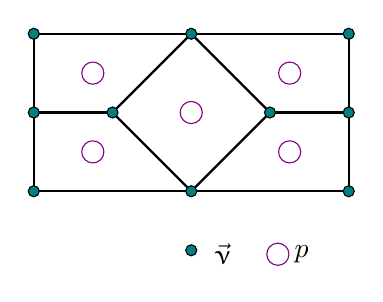
\begin{tikzpicture}
%\draw[fill=gray!23,gray!23](0,0) rectangle (5,5);
%\draw[step=0.5cm,gray,very thin] (0,0) grid (6,4); %background grid
\draw[thick] (1,1) -- (5,1) -- (5,3) -- (1,3) -- cycle;  
\draw[thick] (3,1) -- (4,2) -- (3,3) -- (2,2) -- cycle;  
\draw[thick] (1,2) -- (2,2);  
\draw[thick] (4,2) -- (5,2);  

\draw[black,fill=teal] (1,1) circle (2pt);
\draw[black,fill=teal] (3,1) circle (2pt);
\draw[black,fill=teal] (5,1) circle (2pt);
\draw[black,fill=teal] (1,2) circle (2pt);
\draw[black,fill=teal] (2,2) circle (2pt);
\draw[black,fill=teal] (4,2) circle (2pt);
\draw[black,fill=teal] (5,2) circle (2pt);
\draw[black,fill=teal] (1,3) circle (2pt);
\draw[black,fill=teal] (3,3) circle (2pt);
\draw[black,fill=teal] (5,3) circle (2pt);

\draw[violet] (1.75,1.5) circle (4pt);
\draw[violet] (1.75,2.5) circle (4pt);
\draw[violet] (4.25,1.5) circle (4pt);
\draw[violet] (4.25,2.5) circle (4pt);
\draw[violet] (3,2) circle (4pt);

\draw[black,fill=teal] (3,0.25)   circle (2pt);
\node[] at (3.4,0.2) {$\vec\upnu$};

\draw[violet] (4.1,0.2) circle (4pt); 
\node[] at (4.4,0.2) {$p$};

\end{tikzpicture}
\end{center}




Gresho \& Sani \cite{grsa} state: "For fans of $Q_1\times Q_0$ who want 
guaranteed optimal convergence of both $u$ and $p$ (with however larger error 
constants caused by the distorted shapes?), one way to assure this is
to discretise via the macro elements above, each composed of five $Q_1\times Q_0$
quadrilaterals. Such checkerboard-killer meshes have been employed in practice
by (at least) Bath\'e \cite{chba93}. Both the macro-element and the proof are
due to Stenberg \cite{sten84}."

Chapelle \& Bathe \cite{chba93}: "the numerical inf-sup test is passed for this mesh and in fact,
this behavior was proven analytically (see Brezzi \& Fortin \cite{brfo}, see 
also Le Tallec \& Ruas \cite{leru86}).

\begin{center}
\includegraphics[width=5cm]{images/meshtopos/qizh07}\\
{\captionfont Taken from Qin \& Zhang (2007) \cite{qizh07}.}
\end{center}

Implemented in \stone~78.

\Literature: Fig 3.12 of Elman \etal book \cite{elsw}.

%......................................
\subsubsection{The Le Tallec macro-element} 

This macro-element is introduced in Le Tallec (1981) \cite{leta81}.

\begin{flushright} {\tiny {\color{gray} (tikz\_letallec.tex)}} \end{flushright}
%~~~~~~~~~~~~~~~~~~~~~~~~~~~~~~~~~~~~~~~~~~~~~~~~~~~~~~~~~~~~~~~~~~~~~~~~~~~~~~~~~~~~~~~~~~~~~~~~~~

\begin{center}
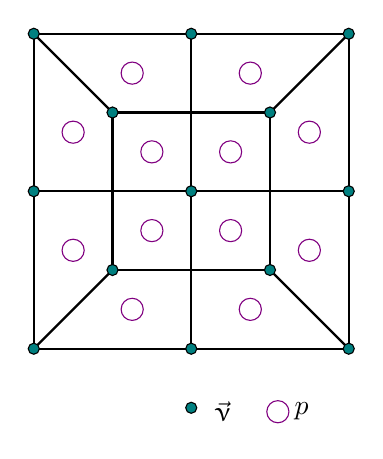
\begin{tikzpicture}
%\draw[fill=gray!23,gray!23](0,0) rectangle (5,5);
%\draw[step=0.5cm,gray,very thin] (0,0) grid (6,6); %background grid
\draw[thick] (1,1) -- (5,1) -- (5,5) -- (1,5) -- cycle;  
\draw[thick] (2,2) -- (4,2) -- (4,4) -- (2,4) -- cycle;  

\draw[thick] (1,1) -- (2,2);  
\draw[thick] (5,1) -- (4,2);  
\draw[thick] (1,5) -- (2,4);  
\draw[thick] (5,5) -- (4,4);  
\draw[thick] (1,3) -- (5,3);  
\draw[thick] (3,1) -- (3,5);  

\draw[black,fill=teal] (1,1)   circle (2pt);
\draw[black,fill=teal] (3,1)   circle (2pt);
\draw[black,fill=teal] (5,1)   circle (2pt);

\draw[black,fill=teal] (2,2)   circle (2pt);
\draw[black,fill=teal] (4,2)   circle (2pt);

\draw[black,fill=teal] (1,3)   circle (2pt);
\draw[black,fill=teal] (3,3)   circle (2pt);
\draw[black,fill=teal] (5,3)   circle (2pt);

\draw[black,fill=teal] (2,4)   circle (2pt);
\draw[black,fill=teal] (4,4)   circle (2pt);

\draw[black,fill=teal] (1,5)   circle (2pt);
\draw[black,fill=teal] (3,5)   circle (2pt);
\draw[black,fill=teal] (5,5)   circle (2pt);

\draw[violet] (2.25,1.5) circle (4pt);
\draw[violet] (3.75,1.5) circle (4pt);

\draw[violet] (1.5,2.25) circle (4pt);
\draw[violet] (1.5,3.75) circle (4pt);
\draw[violet] (2.5,2.5) circle (4pt);
\draw[violet] (3.5,2.5) circle (4pt);
\draw[violet] (2.5,3.5) circle (4pt);
\draw[violet] (3.5,3.5) circle (4pt);
\draw[violet] (4.5,2.25) circle (4pt);
\draw[violet] (4.5,3.75) circle (4pt);
\draw[violet] (2.25,4.5) circle (4pt);
\draw[violet] (3.75,4.5) circle (4pt);

\draw[black,fill=teal] (3,0.25)   circle (2pt);
\node[] at (3.4,0.2) {$\vec\upnu$};

\draw[violet] (4.1,0.2) circle (4pt); 
\node[] at (4.4,0.2) {$p$};

\end{tikzpicture}\\
\end{center}




This macro-element has been proven stable in \cite{leta81,leru86}, i.e. it satisfies 
the stability condition (see Section~\ref{ss:pair}).
It is also mentioned in Qin \& Zhang (2007) \cite{qizh07}.

Implemented in \stone 78.

%..............................................
\subsubsection{The Qin \& Zhang macro-elements}

In their paper Qin \& Zhang (2007) \cite{qizh07} the authors mention the Stenberg and Le Tallec
macro-elements and also introduce three new ones:

\begin{minipage}{0.31\textwidth}
\begin{flushright} {\tiny {\color{gray} (tikz\_qizh07a.tex)}} \end{flushright}
%~~~~~~~~~~~~~~~~~~~~~~~~~~~~~~~~~~~~~~~~~~~~~~~~~~~~~~~~~~~~~~~~~~~~~~~~~~~~~~~~~~~~~~~~~~~~~~~~~~

\begin{center}
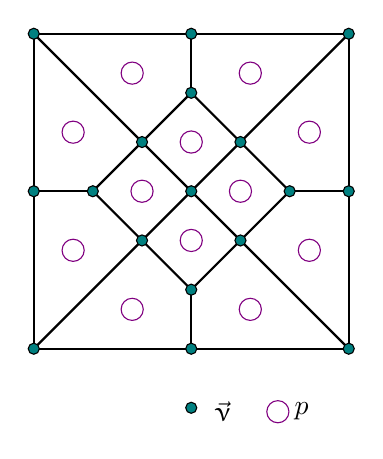
\begin{tikzpicture}
%\draw[fill=gray!23,gray!23](0,0) rectangle (5,5);
%\draw[step=0.5cm,gray,very thin] (0,0) grid (6,6); %background grid
\draw[thick] (1,1) -- (5,1) -- (5,5) -- (1,5) -- cycle;  
\draw[thick] (1.75,3) -- (3,1.75) -- (4.25,3) -- (3,4.25) -- cycle;  

\draw[thick] (1,1) -- (5,5) ;  
\draw[thick] (1,5) -- (5,1) ;  

\draw[thick] (3,1) -- (3,1.75) ;  
\draw[thick] (3,4.25) -- (3,5) ;  

\draw[thick] (1,3) -- (1.75,3) ;  
\draw[thick] (4.25,3) -- (5,3) ;  

\draw[black,fill=teal] (1,1)   circle (2pt);
\draw[black,fill=teal] (3,1)   circle (2pt);
\draw[black,fill=teal] (5,1)   circle (2pt);

\draw[black,fill=teal] (3,1.75)   circle (2pt);
\draw[black,fill=teal] (2.375,2.375)   circle (2pt);
\draw[black,fill=teal] (3.625,2.375)   circle (2pt);

\draw[black,fill=teal] (1,3)   circle (2pt);
\draw[black,fill=teal] (1.75,3)   circle (2pt);
\draw[black,fill=teal] (3,3)   circle (2pt);
\draw[black,fill=teal] (4.25,3)   circle (2pt);
\draw[black,fill=teal] (5,3)   circle (2pt);

\draw[black,fill=teal] (2.375,3.625)   circle (2pt);
\draw[black,fill=teal] (3.625,3.625)   circle (2pt);
\draw[black,fill=teal] (3,4.25)   circle (2pt);

\draw[black,fill=teal] (1,5)   circle (2pt);
\draw[black,fill=teal] (3,5)   circle (2pt);
\draw[black,fill=teal] (5,5)   circle (2pt);

\draw[violet] (2.25,1.5) circle (4pt);
\draw[violet] (3.75,1.5) circle (4pt);

\draw[violet] (1.5,2.25) circle (4pt);
\draw[violet] (3,2.375) circle (4pt);
\draw[violet] (4.5,2.25) circle (4pt);

\draw[violet] (2.375,3) circle (4pt);
\draw[violet] (3.625,3) circle (4pt);

\draw[violet] (3,3.625) circle (4pt);
\draw[violet] (1.5,3.75) circle (4pt);
\draw[violet] (4.5,3.75) circle (4pt);

\draw[violet] (2.25,4.5) circle (4pt);
\draw[violet] (3.75,4.5) circle (4pt);

\draw[black,fill=teal] (3,0.25)   circle (2pt);
\node[] at (3.4,0.2) {$\vec\upnu$};

\draw[violet] (4.1,0.2) circle (4pt); 
\node[] at (4.4,0.2) {$p$};
\end{tikzpicture}\\
\end{center}


\end{minipage}\hfill 
\begin{minipage}{0.31\textwidth}
\begin{flushright} {\tiny {\color{gray} (tikz\_qizh07b.tex)}} \end{flushright}
%~~~~~~~~~~~~~~~~~~~~~~~~~~~~~~~~~~~~~~~~~~~~~~~~~~~~~~~~~~~~~~~~~~~~~~~~~~~~~~~~~~~~~~~~~~~~~~~~~~

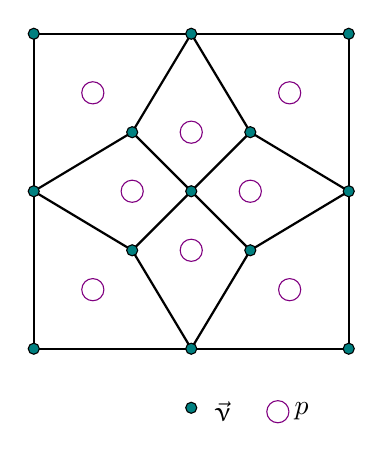
\begin{tikzpicture}

%\draw[fill=gray!23,gray!23](0,0) rectangle (5,5);
%\draw[step=0.5cm,gray,very thin] (0,0) grid (6,6); %background grid
\draw[thick] (1,1) -- (5,1) -- (5,5) -- (1,5) -- cycle;  
\draw[thick] (1,3) -- (2.25,2.25) -- (3,1) -- (3.75,2.25) -- (5,3) --(3.75,3.75) -- (3,5) --(2.25,3.75) --cycle;  
\draw[thick] (2.25,2.25) -- (3.75,3.75) ;  %diags
\draw[thick] (2.25,3.75) -- (3.75,2.25) ;  

\draw[black,fill=teal] (1,1)   circle (2pt); %perimeter nodes
\draw[black,fill=teal] (3,1)   circle (2pt);
\draw[black,fill=teal] (5,1)   circle (2pt);
\draw[black,fill=teal] (1,3)   circle (2pt);
\draw[black,fill=teal] (3,3)   circle (2pt);
\draw[black,fill=teal] (5,3)   circle (2pt);
\draw[black,fill=teal] (1,5)   circle (2pt);
\draw[black,fill=teal] (3,5)   circle (2pt);
\draw[black,fill=teal] (5,5)   circle (2pt);

\draw[black,fill=teal] (2.25,2.25)   circle (2pt); %inside nodes
\draw[black,fill=teal] (3.75,3.75)   circle (2pt);
\draw[black,fill=teal] (2.25,3.75)   circle (2pt);
\draw[black,fill=teal] (3.75,2.25)   circle (2pt);

\draw[violet] (1.75,1.75) circle (4pt);
\draw[violet] (4.25,1.75) circle (4pt);
\draw[violet] (4.25,4.25) circle (4pt);
\draw[violet] (1.75,4.25) circle (4pt);

\draw[violet] (3,2.25) circle (4pt);
\draw[violet] (3,3.75) circle (4pt);
\draw[violet] (2.25,3) circle (4pt);
\draw[violet] (3.75,3) circle (4pt);

%------------------------------------------
\draw[black,fill=teal] (3,0.25)   circle (2pt);
\node[] at (3.4,0.2) {$\vec\upnu$};
\draw[violet] (4.1,0.2) circle (4pt); 
\node[] at (4.4,0.2) {$p$};


\end{tikzpicture}\\

\end{minipage}\hfill 
\begin{minipage}{0.31\textwidth}
\begin{flushright} {\tiny {\color{gray} (tikz\_qizh07c.tex)}} \end{flushright}
%~~~~~~~~~~~~~~~~~~~~~~~~~~~~~~~~~~~~~~~~~~~~~~~~~~~~~~~~~~~~~~~~~~~~~~~~~~~~~~~~~~~~~~~~~~~~~~~~~~


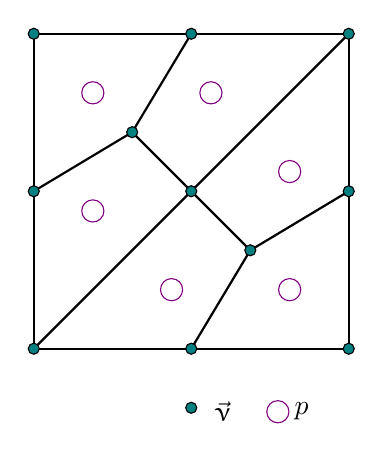
\begin{tikzpicture}
%\draw[fill=gray!23,gray!23](0,0) rectangle (5,5);
%\draw[step=0.5cm,gray,very thin] (0,0) grid (6,6); %background grid
\draw[thick] (1,1) -- (5,1) -- (5,5) -- (1,5) -- cycle;  
\draw[thick] (1,3) -- (2.25,3.75) -- (3,5);
\draw[thick] (3,1) -- (3.75,2.25) -- (5,3);
\draw[thick] (1,1) -- (5,5) ;  %diags
\draw[thick] (2.25,3.75) -- (3.75,2.25) ;  

\draw[black,fill=teal] (1,1)   circle (2pt); %perimeter nodes
\draw[black,fill=teal] (3,1)   circle (2pt);
\draw[black,fill=teal] (5,1)   circle (2pt);
\draw[black,fill=teal] (1,3)   circle (2pt);
\draw[black,fill=teal] (3,3)   circle (2pt);
\draw[black,fill=teal] (5,3)   circle (2pt);
\draw[black,fill=teal] (1,5)   circle (2pt);
\draw[black,fill=teal] (3,5)   circle (2pt);
\draw[black,fill=teal] (5,5)   circle (2pt);

\draw[black,fill=teal] (2.25,3.75)   circle (2pt); %inside nodes
\draw[black,fill=teal] (3.75,2.25)   circle (2pt);

\draw[violet] (4.25,1.75) circle (4pt);
\draw[violet] (1.75,4.25) circle (4pt);

\draw[violet] (2.75,1.75) circle (4pt);
\draw[violet] (4.25,3.25) circle (4pt);
\draw[violet] (1.75,2.75) circle (4pt);
\draw[violet] (3.25,4.25) circle (4pt);

%------------------------------------------
\draw[black,fill=teal] (3,0.25)   circle (2pt);
\node[] at (3.4,0.2) {$\vec\upnu$};
\draw[violet] (4.1,0.2) circle (4pt); 
\node[] at (4.4,0.2) {$p$};
\end{tikzpicture}


\end{minipage}

They also indicate that although stable, these macro-elements are inferior 
to the above two (Stenberg \& Le Tallec). 

%..............................................
\subsubsection{New macro-elements ?}

\begin{center}
\includegraphics[width=4cm]{images/meshtopos/m21}
\includegraphics[width=4cm]{images/meshtopos/m22}
\end{center}

I came up with these, no idea whether these are stable/usable or better than the others.






 

 %------------------
\newpage
\section{Solving the Stokes system \label{sec:solvers}} \begin{flushright} {\tiny {\color{gray} \tt solvers.tex}} \end{flushright}
%~~~~~~~~~~~~~~~~~~~~~~~~~~~~~~~~~~~~~~~~~~~~~~~~~~~~~~~~~~~~~~~~~~~~~~~~~~~~~~~~~~~~~~~~~~~~~~~~~~

Let us start again from the (full) Stokes system:
\begin{equation}
\underbrace{
\left(
\begin{array}{cc}
\K & \G \\ \G^T & -\C 
\end{array}
\right)
}_{\cal A}
\cdot
\left(
\begin{array}{c}
\vec{\cal V} \\ \vec{\cal P}
\end{array}
\right)
=
\left(
\begin{array}{c}
\vec{f} \\ \vec{h}
\end{array}
\right)
\label{StokesSyst}
\end{equation}
We need to solve this system in order to obtain the solution, i.e. the $\vec{\cal V}$ 
and $\vec{\cal P}$ vectors. But how? 
Unfortunately, this question is not simple to answer and the appropriate method depends on many 
parameters, but mainly on how big the matrix blocks are and what the condition number of the matrix $\K$ is. 

First let us start with an obvious question: couldn't we just compute the inverse of the matrix ${\cal A}$?
Under the assumption that the inverse of $\K$ and $\SSS$ exists, we can and we find\footnote{The matrix 
$\C$ is here omitted but it bears no consequences on the conclusion.}
\[
{\cal A}^{-1} = 
\left(
\begin{array}{cc}
\K & \G \\ \G^T & 0
\end{array}
\right)^{-1}
=
\left(
\begin{array}{cc}
\K^{-1} + \K^{-1} \cdot \G \cdot\SSS^{-1} \cdot\G^T \cdot\K^{-1} & -\K^{-1} \cdot\G \cdot\SSS^{-1} \\ 
-\SSS^{-1} \cdot\G^T \cdot\K^{-1}  &  \SSS^{-1}
\end{array}
\right)
\]
However, such an expression is of limited interest in the numerical solution of saddle
point problems since it showcases 5 times the inverse of $\K$ and more importantly
the inverse of the Schur complement matrix $\SSS$ which is likely to be a full matrix so 
that we never want to compute it explicitely.


As concisely explained in Clevenger \& Heister (2021) \cite{clhe21}, 
there are three common approaches used in the literature for solving the above equation on large scales:
\begin{itemize}
\item a pressure corrected, Schur complement CG scheme, using multigrid as an 
approximation to the velocity block;
\item a block-preconditioned Krylov
method, also using multigrid on the velocity block.
For this method, there are two main types:
\begin{itemize}
\item GMRES\cite{mabl15,rumi15} (or any Krylov method not requiring symmetry) with
block-triangular preconditioner (This is what \aspect does):
\[
{\bm P} = \left(
\begin{array}{cc}
\K & \G \\
0 & - \SSS
\end{array}
\right)
\]

\item MINRES\cite{gmhj16} with block-diagonal preconditioner
\[
{\bm P} = \left(
\begin{array}{cc}
\K & 0 \\
0 & - \SSS
\end{array}
\right)
\]

\end{itemize}

\item an all-at-once multigrid performed on the entire Stokes system, using Uzawa-type smoothers.
\end{itemize}



\Literature: Preconditioners for Incompressible Navier-Stokes Solvers 
\begin{small}
\begin{itemize}
\item \fullcite{benz02}
\item \fullcite{bewa08}
\item \fullcite{urvs08}
\item \fullcite{seuv10}
\item Saddle point preconditioners have been extensively discussed and studied \cite{bewa08}, \cite{dewu04}
\item Diagonal preconditioners in \cite{shrb01}, \cite{babc94}.
\end{itemize}
\end{small}

\Literature: Solving Stokes Saddle Point problem
\begin{small}
\begin{itemize}
\item \fullcite{laqu86}
\item \fullcite{rotf90}
\item \fullcite{frha93}
\item \fullcite{elgo94}
\item \fullcite{cheb96}, \fullcite{elma96}
\item \fullcite{brpv97}
\item \fullcite{lixu01}
\item \fullcite{dogs06}, \fullcite{lica06}
\item \fullcite{hoow17}
\item Pragmatic solvers for 3D Stokes problems with heterogeneous coefficients \cite{samb20}
\end{itemize}
\end{small}



%------------------------------------------------------------------------------
\subsection{Block diagonal scaling} \label{sec:block_scaling}

We have already seen in Section~\ref{pscaling} how and why we scale the $\G$ block. 
We revisit this topic more thoroughly in what follows.
This section is borrowed from Section~2.6 of \textcite{mamo08} (2008).

Let us state again the equation we wish to solve (Eq. 6 in the paper):
\[
\begin{pmatrix}
\K & \G \\
\G^T & 0
\end{pmatrix}
\cdot
\begin{pmatrix}
\vec{\cal V} \\
\vec{\cal P}
\end{pmatrix}
=
\begin{pmatrix}
\vec{f} \\
\vec{h}
\end{pmatrix}
\]

Prior to solving this equation, the autors apply a row/column scaling to the equation
to effectively normalize the operators $\K$ and $\G$ with the intention of
reducing round off errors. The scaling is particularly important for
problems in geodynamics when dimensional quantities are used to
define the problem and because of the large, local variations which
may occur in the constitutive tensor (in practice, the effective viscosity) . 

They apply a symmetric block diagonal scaling to the equation via the scaling matrix\footnote{
The $S$ stands for 'scaling', the Schur complement is given by $\SSS$}
\[
{\bm S} = 
\begin{pmatrix}
{\bm S}_1 & 0 \\ 0 & {\bm S}_2
\end{pmatrix}
\]
Writing the first equation as ${\bm A} \cdot \vec{x} = \vec{b}$, 
the symmetric scaling operation is applied as follows:
\[
{\bm S}^{-1} \cdot {\bm A} \cdot \vec{x}= {\bm S}^{-1} \cdot \vec{b} 
\]
followed by\footnote{${\bm S}^{-T}$ is the inverse of the transpose of the matrix.} 
\[
{\bm S}^{-1} \cdot {\bm A} \cdot {\bm S}^{-T} \cdot {\bm S}^T \cdot \vec{x}= {\bm S}^{-1} \cdot \vec{b} 
\]
to give the scaled system ${\bm A}_s \cdot \vec{y}_s = \vec{b}_s$ , where the operator 
${\bm A}_s$ is given by
\begin{eqnarray}
{\bm S}^{-1} \cdot {\bm A} \cdot {\bm S}^{-T} 
&=&\begin{pmatrix}
{\bm S}_1^{-1} & 0 \\ 0 & {\bm S}_2^{-1}
\end{pmatrix}
\cdot 
\begin{pmatrix}
\K & \G \\
\G^T & 0
\end{pmatrix}
\cdot
\begin{pmatrix}
{\bm S}_1^{-T} & 0 \\ 0 & {\bm S}_2^{-T}
\end{pmatrix} \nn\\
&=&
\begin{pmatrix}
{\bm S}_1^{-1} \cdot \K \cdot {\bm S}_1^{-T} & {\bm S}_1^{-1} \cdot \G \cdot {\bm S}_2^{-T} \\
({\bm S}_1^{-1} \cdot \G \cdot {\bm S}_2^{-T})^{T} & 0 
\end{pmatrix} \nn\\
&=&
\begin{pmatrix}
\K_s & \G_s \\
\G^T_s & 0
\end{pmatrix} \nn\\
&=&{\bm A}_s \nn
\end{eqnarray}
with
\[
{\bm S}^T \cdot \vec{x} 
= 
\begin{pmatrix}
{\bm S}_1^T \cdot \vec{\cal V} \\
{\bm S}_2^T \cdot \vec{\cal P}
\end{pmatrix}
=\vec{y}_s
\qquad\qquad
{\bm S}^{-1} \cdot \vec{b} = 
\begin{pmatrix}
{\bm S}_1^{-1}\cdot\vec{f} \\
{\bm S}_2^{-1}\cdot\vec{h}
\end{pmatrix}
=\vec{b}_s
\]
Following the solution of the scaled system, we recover the un-scaled
solution from $\vec{x} = {\bm S}^{-T} \cdot  \vec{y}_s$. 
The form of the scaling operation is based
on the preconditioner described in Rusten and Winther (1992). For
the purpose of scaling, rather than full preconditioning of the indefinite system, 
we let both ${\bm S}_1$ and ${\bm S}_2$ be diagonal matrices. We seek
to approximately normalize the operators $\K$ and $\G$.

Thus we let 
\[
S_1(i,i) = \sqrt{ \max_j K_{ij}} \qquad \forall i \in [1,NfemV]
\]
The choice for ${\bm S}_2$ is based on the requirement that $\G^T_s\cdot \G_s \simeq {\bm 1}_{Nfemp}$ (i.e.
the identity matrix of size $NfemP\times NfemP$) which yields the relation
\[
\G^T_s \cdot \G = ({\bm S}_1^{-1} \cdot \G \cdot {\bm S}_2^{-T})^T 
\cdot ({\bm S}_1^{-1} \cdot \G \cdot {\bm S}_2^{-T} )
= {\bm S}_2^{-1} \cdot \G^T \cdot {\bm S}_1^{-T} \cdot {\bm S}_1^{-1} \cdot \G \cdot {\bm S}_2^{-T} = {\bm 1}
\]
We can left multiply by ${\bm S}_2$ and right multiply by  ${\bm S}_2^T$ to obtain
\[
\G^T \cdot {\bm S}_1^{-T} \cdot {\bm S}_1^{-1} \cdot \G = {\bm S}_2 \cdot {\bm S}_2^T
\]
We can approximately satisfy this equation if we first define the vector $\vec{g}$ of size $NfemV$
\[
g_i = \max_j(G_{ij}) 
\]
and then let
\[
S_2(i,i)=\frac{1}{NfemV} \sqrt{ \left( \sum_k S_1^2(k,k) \right)   \vec{g}_i \cdot \vec{g}_i}
\]
Note that in the paper the above equation (their eq.37) does not contain any $i$ in the rhs, 
which is probably missing from the $\vec{g}$ vectors.


{\color{red} sent email to Dave May 15/01/2026}



%...................................................
\subsection{When using the penalty formulation}

In this case we are only solving for velocity since pressure has been eliminated 
and is later recovered in a post-processing step. The linear system is of the form:
\[
(\K_\eta+\K_\lambda) \cdot \vec {\cal V} = \vec f
\]
 We also know that 
the penalty factor $\lambda$ is many orders of magnitude higher than the viscosity and 
in combination with the use of the $Q_1 \times P_0$ element the resulting matrix 
condition number is very high so that the use of iterative solvers is precluded. 
Indeed codes such as \sopale \cite{full95}, \douar \cite{brtf08}, \fantom \cite{thie11} 
or \sulec \cite{qube11} relying on the penalty formulation all use direct solvers.
The most popular are BLKFCT\footnote{\url{http://dm.unife.it/blkfclt/}}, 
MUMPS\footnote{\url{http://mumps.enseeiht.fr/}}\cite{amdu89,amdl00,amdk01,amgl06,ambl19}, 
PasTiX \cite{herr02},
WSMP\footnote{\url{http://www.research.ibm.com/projects/wsmp}} \cite{GUPTA94ieee,GUPTA09sc-long},
UMFPACK and CHOLMOD\footnote{\url{http://faculty.cse.tamu.edu/davis/suitesparse.html}}
, SuperLU\footnote{\url{https://portal.nersc.gov/project/sparse/superlu/}}, 
PARDISO\footnote{\url{https://www.pardiso-project.org/}}
\cite{pardiso-6.0a,pardiso-6.0b,pardiso-6.0c}, or those inside 
PETSc\footnote{\url{https://www.mcs.anl.gov/petsc/}}.

Braun \etal (2008) \cite{brtf08} list the following features of direct solvers:
\begin{itemize}
\item Robust
\item Black-box operation
\item Difficult to parallelize
\item Memory consumption
\item Limited scalability
\end{itemize}

The main advantage of direct solvers is used in this case: They can solve ill-conditioned 
matrices. However, memory requirements for the storage of number of nonzeros in the 
Cholesky matrix grow very fast as the number of equations/grid size increases, especially in 3D,
to the point that even modern computers with tens of Gb of RAM cannot deal with a $\sim 100^3$ element mesh.
This explains why direct solvers are often used for 2D problems and rarely in 3D with noticeable 
exceptions \cite{thfb08,yahb09,brya10,lobh10,alht11,alht12,alhf13,whbb14,neew18}. 

Note that \textcite{pedr24} (2024) conducted a detailed study comapring 
MUMPS, UMFPACK, and Intel DSS (PARDISO).
The conclusions are 
\begin{displayquote}
{\color{darkgray}
1. Intel DSS is not ready for production codes because it computes incorrect results without warnings;\\
2. UMFPACK reaches the memory limit earlier than the other solvers and must be configured with the automatic
symmetry strategy to yield correct results; and\\
3. MUMPS is not thread-safe and, in particular, does not work well with OpenBLAS, which causes thread 'locks' and
conflicts. However, MUMPS works well with Intel MKL and is the only solver able to tackle massive systems.}
\end{displayquote}
In \textcite{saramito} we find the following table whigh gives the aymptotic computing time versus the 
size of the sparse matrix $n$ and the geometry dimension $d$:
\[
\begin{array}{lcc}
d& \text{factorize} & \text{solve} \\
\hline\hline
1& n & n \\
2& n^{3/2} & n \log n \\
3& n^2 & n^{4/3}\\
\hline
\end{array}
\]

%....................................................................
\subsection{Uzawa algorithms and the Schur complement approach }

\index{general}{Uzawa algorithm}

Let us write the above system as two equations:
\begin{eqnarray}
\K \cdot \vec{\cal V} + \G \cdot \vec{\cal P} &=& \vec{f} \nn\\
\G^T \cdot  \vec{\cal V} - \C \cdot \vec{\cal P} &=& \vec{h} \nn
\end{eqnarray}
Again, $\C$ is typically non-zero in the case of stabilised elements or if a 
penalty formulation is used. 
The first line can be re-written 
$\vec{\cal V}=\K^{-1}\cdot (\vec{f} - \G \cdot \vec{\cal P})$ and can be inserted in the second:
\begin{equation}
\G^T\cdot \vec{\cal V} =\G^T \cdot  [ \K^{-1} \cdot  (\vec{f} - \G \cdot  \vec{\cal P}) ] - \C\cdot \vec{\cal P} = \vec{h} 
\end{equation}
which can be written: 
\begin{mdframed}[backgroundcolor=blue!5]
\begin{equation}
(\G^T \cdot \K^{-1} \cdot \G + \C) \cdot \vec{\cal P} = \G^T \cdot \K^{-1}\cdot \vec{f} - \vec{h} 
\end{equation}
\end{mdframed}
The matrix $\SSS= \G^T \cdot \K^{-1} \cdot \G + \C$ is called the Schur complement. 
\index{general}{Schur Complement} 
It is Symmetric (since $\K$ is symmetric) and  Positive-Definite\footnote{$M$ 
positive definite $\iff$ $x^TMx>0$ $\forall \; x\in \mathbb{R}^n \setminus {\bm 0}$ }
(SPD) \index{general}{SPD} if $Ker({\G})=0$. 
Having solved this equation (i.e. we have obtained $\vec{\cal P}$), the velocity can be recovered by solving 
$\K\cdot \vec{\cal V} =\vec{f}- \G \cdot \vec{\cal P}$. 

\begin{remark}
The Schur complement matrix naturally occurs when the Stokes matrix is decomposed using 
a LDU block-factorisation. Indeed, we have 
\[
\left(
\begin{array}{cc}
\K & \G \\ 
\G^T & 0
\end{array}
\right)
=
\left(
\begin{array}{cc}
{\bm I} & 0 \\ 
\G^T \cdot \K^{-1} & {\bm I}
\end{array}
\right)
\cdot
\left(
\begin{array}{cc}
\K & 0 \\ 
0 & -\SSS
\end{array}
\right)
\cdot
\left(
\begin{array}{cc}
{\bm I} & \K^{-1} \cdot \G \\ 
0 & {\bm I}
\end{array}
\right)
\]
\end{remark}

For now, let us assume that we have built the $\SSS$ matrix\footnote{We will 
revisit this topic later on, but be aware that we never build $\SSS$ in practice.} 
and the right hand 
side $\underline{\vec{f}}=\G^T \cdot \K^{-1} \cdot \vec{f} - \vec{h}$.
We must then solve $\SSS\cdot \vec{\cal P} = \underline{\vec{f}}$.
It is easy to see that $\SSS$ is actually a full matrix (i.e. not sparse) and 
aside from the costs of building it, explicitly using a direct solver would require 
a lot (i.e. too much in practice) of memory so that we must then turn to iterative methods. 

\index{general}{Richardson Iterations}
One can resort to so-called Richardson iterations, defined as follows 
(e.g., see Varga \cite{varga}, p141):
in solving the matrix equation ${\bm A}\cdot {\vec X}={\vec b}$,
the Richardson iterative method is defined by: 
\begin{equation}
{\vec X}_{k+1} = {\vec X}_k + \alpha_k (-{\bm A} \cdot {\vec X}_k + {\vec b})
\quad\quad
m\geq 0 
\end{equation}
where the $\alpha_k$'s are real scalars. 
It is easy to see that when the method converges then ${\vec X}_{k+1} \simeq {\vec X}_k$  and then 
for $\alpha_k\neq 0$ then ${\bm A}\cdot {\vec X}={\vec b}$ is satisfied. 
In our case, it writes:
\begin{eqnarray}
\vec {\cal P}_{k+1} 
&=& \vec {\cal P}_{k} + \alpha_k ( - \SSS \cdot \vec{\cal P}_{k}  +  \underline{\vec{f}}) \nonumber\\
&=& \vec {\cal P}_{k} + \alpha_k \left[ - (\G^T \cdot \K^{-1} \cdot \G + \C)  \cdot \vec{\cal P}_{k} 
+  (\G^T \cdot \K^{-1} \cdot \vec{f} - \vec{h}   ) \right] \nonumber\\
&=& \vec {\cal P}_{k} + \alpha_k \left[ \G^T \cdot \K^{-1} \cdot ( - \G \cdot \vec{\cal P}_{k} + \vec{f}) 
-\C \cdot \vec{\cal P}_{k} - \vec{h} 
\right] \nonumber\\
&=& \vec {\cal P}_{k} + \alpha_k \left[ \G^T \cdot \K^{-1} \cdot ( \K\cdot \vec{\cal V}_k)
-\C \cdot \vec{\cal P}_{k}  - \vec{h} \right] \nonumber\\
&=& \vec {\cal P}_{k} + \alpha_k \left( \G^T \cdot \vec{\cal V}_k -\C \cdot \vec{\cal P}_{k} - \vec{h} \right) 
\end{eqnarray}
The above iterations are then carried out and for each new pressure field the associated velocity field 
is computed. The method of using Richardson iterations applied to the Schur complement 
is commonly called the Uzawa algorithm (see Braess \cite[p221]{braess}
\footnote{I have slightly 
altered the indices of the velocities wrt the book}).

\begin{mdframed}[backgroundcolor=blue!5]
\underline{\bf Uzawa algorithm (1)}: assume $\vec{\cal P}_0$ known
\begin{eqnarray}
\text{solve} \qquad \mathbb{K} \cdot \vec{\cal V}_k &=& \vec f - \mathbb{G}\cdot \vec {\cal P}_{k} \\
\vec{\cal P}_{k+1} &=& 
\vec{\cal P}_{k}  + \alpha_k (\mathbb{G}^T\cdot \vec{\cal V}_k  -\C \cdot \vec{\cal P}_{k} -\vec h)
\quad
\quad
\quad
\quad
k=0,1,2, ... \label{uzaa2}
\end{eqnarray}
\end{mdframed}
This same algorithm is to be found on page 59 of \cite{saramito}.

This method is rather simple to implement, although
what makes an appropriate set of $\alpha_k$ values is not 
straightforward, which is why the conjugate gradient method (or any method
which computes an optimal $\alpha_k$ in some sense) is often preferred, 
as detailed in the next section. 

It is known that such iterations will converge for $0< \alpha < \rho(\SSS)= \lambda_{max}(\SSS)$ 
where $\rho(\SSS)$ is the spectral radius of the matrix $\SSS$
which is essentially the largest, in absolute value, eigenvalue of $\SSS$ (neither of which 
can be computed easily).  
It can also be proven that the rate of convergence depends on the condition number of the matrix.

Richardson iterations are part of the family of stationary iterative 
methods\footnote{\url{https://mathworld.wolfram.com/StationaryIterativeMethod.html}}, 
since it can be rewritten 
\begin{equation}
{\vec X}_{k+1} = ({\bm I} - \alpha_k {\bm A} ) \cdot {\vec X}_k + \alpha_k {\vec b}
\end{equation}
which is the definition of a stationary method. 
The four main stationary methods are the Jacobi method, 
Gauss-Seidel method, successive overrelaxation method (SOR), 
and symmetric successive overrelaxation method (SSOR).
\index{general}{Jacobi Iterative Method}
\index{general}{Gauss-Seidel Iterative Method}
\index{general}{SOR Iterative Method}
\index{general}{SSOR Iterative Method}

Since the $\alpha$ parameter is the key to a successful Uzawa algorithm, 
this issue has of course been investigated. What follows is 
presented in p221 of Braess \cite{braess}.
For the analysis of the Uzawa algorithm, we define the residual
\[
\vec {\cal R}_k = \vec h - \mathbb{G}^T \cdot \vec{\cal V}_k  +\C \cdot \vec{\cal P}_{k}
\]
In addition, suppose the solution of the saddle point problem is denoted
by $(\vec{\cal V}^\star,\vec{\cal P}^\star)$ so that we have
\[
\vec{f} = \K \cdot \vec{\cal V}^\star + \G \cdot \vec{\cal P}^\star
\qquad
{\rm and}
\qquad
\vec{h} = \G^T \cdot \vec{\cal V}^\star - \C \cdot \vec{\cal P}^\star 
\]

Now substituting the iteration formula for ${\cal V}_k$, and inserting $\vec{f}$ and $\vec{h}$ from above,
we get
\begin{eqnarray}
\vec{\cal R}_k 
&=& \vec{h} -\G^T  \cdot \vec{\cal V}_k  +\C \cdot \vec{\cal P}_{k} \nn\\
&=& \vec{h} -\mathbb{G}^T\cdot \mathbb{K}^{-1} (\vec f - \mathbb{G}\cdot \vec{\cal P}_{k})  +\C \cdot \vec{\cal P}_{k}\nn\\
&=& (\G^T\cdot\vec{\cal V}^\star - \C \cdot \vec{\cal P}^\star) -\mathbb{G}^T\cdot \mathbb{K}^{-1} (\K\cdot\vec{\cal V}^\star 
+ \G\cdot\vec{\cal P}^\star - {\G}\cdot \vec{\cal P}_{k})+\C \cdot \vec{\cal P}_{k} \nn\\
&=& ({\G}^T \cdot \mathbb{K}^{-1} \cdot \mathbb{G} + \C)\cdot (\vec {\cal P}_{k} - \vec{\cal P}^\star) 
\end{eqnarray}
From Eq.~\eqref{uzaa2} it follows that:
\begin{eqnarray}
\vec{\cal P}_{k+1} - \vec{\cal P}_{k}  
&=& \alpha\; (\mathbb{G}^T\cdot \vec{\cal V}_k -\C \cdot \vec{\cal P}_{k} -\vec h) \\
&=& -\alpha\; \vec{\cal R}_k \\ 
&=& -\alpha\; ( \mathbb{G}^T \cdot \mathbb{K}^{-1} \cdot \mathbb{G} + \C )
\cdot (\vec {\cal P}_{k} -\vec{\cal P}^\star)\\ 
&=& \alpha\; (\mathbb{G}^T \cdot \mathbb{K}^{-1} \cdot \mathbb{G} + \C) \cdot 
(\vec{\cal P}^\star - \vec {\cal P}_{k} ) 
\end{eqnarray}
Thus the Uzawa algorithm is equivalent to applying the gradient method 
to the reduced equation using a fixed step size. 
In particular, the iteration converges for
$
\alpha < 2 || \G^T \cdot \K^{-1} \cdot \G + \C||^{-1}
$
and one can show that the good step size $\alpha_k$ is given by\footnote{I need to include matrix $\C$.}
\begin{equation}
\alpha_k = \frac{\vec{\cal R}_k \cdot \vec{\cal R}_k}
{(\G \cdot \vec{\cal R}_k)\cdot (\K^{-1}\cdot \G \cdot \vec{\cal R}_k)}
\label{uzaa3}
\end{equation}



However, if we were to use this rule formally, we would 
need an additional multiplication by $\K^{-1}$ in every step 
of the iteration. This can be avoided by storing an 
auxiliary vector. 
Note that this algorithm is presented in Zienkiewicz \etal (1985) \cite{zivt85} 
in the context of viscoplastic flow.

%Note that in \cite{glow} it is stated: the convergence of this algorithm is proved for 
%$\alpha \in (0,2\mu/d)$ (where $d$ is the number of dimensions).
%\todo[inline]{check this, and report page number}

As mentioned above, there is a way to rework the original Uzawa algorithm 
to include Eq. (\ref{uzaa3}). It is yields a modified 
Uzawa algorithm (see p222 of Braess \cite{braess}
\footnote{I have slightly 
altered the indices of the velocities wrt the book}):


\begin{mdframed}[backgroundcolor=blue!5]
\underline{\bf Uzawa algorithm (2)}: assume $\vec{\cal P}_0$ known. 
Solve $\mathbb{K}\cdot \vec{\cal V}_0 = \vec f - \mathbb{G}\cdot  \vec{\cal P}_0$. 
For $k=0,1,2,...$, compute 
\begin{eqnarray}
\vec{\cal R}_k=\vec q_k &=& \vec h-\mathbb{G}^T \cdot \vec{\cal V}_k + \C \cdot \vec{\cal P}_{k}\\
\vec{p}_k &=& {\G}\cdot q_k \\
\vec H_k &=& {\K}^{-1}\cdot \vec{p}_k \\
\alpha_k &=& \frac{\vec q_k \cdot \vec q_k}{\vec{p}_k \cdot \vec H_k} \\
\vec {\cal P}_k &=& \vec {\cal P}_{k-1} - \alpha_k  \vec q_k \\
\vec {\cal V}_{k} &=& \vec {\cal V}_{k-1} + \alpha_k  \vec H_k
\end{eqnarray}
\end{mdframed}


\Literature: \\
\begin{itemize}
\item
\fullcite{cach88}
\item
\fullcite{bamn02}
\item
\fullcite{cao03}
\item
\fullcite{kosa11}
\end{itemize}

These Uzawa methods have been implemented in \stone~147.


\newpage
%...................................................
\subsection{Conjugate gradient and the Schur complement approach }
\label{ss:schurpcg}

\index{general}{CG} \index{general}{Conjugate Gradient}
Since the Schur matrix $\SSS$ is Symmetric Positive Definite, 
the Conjugate Gradient (CG) 
method\footnote{\url{https://en.wikipedia.org/wiki/Conjugate_gradient_method}} \cite{hest52} 
is very appropriate to solve this system. 

Indeed, looking at the definition of Wikipedia: "{\it In mathematics, the conjugate 
gradient method is an algorithm for the numerical solution of particular systems of 
linear equations, namely those whose matrix is symmetric and positive-definite. 
The conjugate gradient method is often implemented as an iterative algorithm, applicable 
to sparse systems that are too large to be handled by a direct implementation or other 
direct methods such as the Cholesky decomposition. 
Large sparse systems often arise when numerically solving partial differential 
equations or optimization problems.}"

See also the excellent document by J. Shewchuk entitled {\it 
An Introduction to the Conjugate Gradient Method Without the Agonizing Pain}
available at \url{https://www.cs.cmu.edu/~quake-papers/painless-conjugate-gradient.pdf}.

A simple Wikipedia search (crossed-checked against other online sources) 
tells us that the Conjugate Gradient algorithm is as follows:

\vspace{0.4cm}

\begin{minipage}{0.48\textwidth}
\centering
{\captionfont Algorithm as obtained from Wikipedia.}\\
\frame{\includegraphics[width=8cm]{images/solvers/cgwiki}}
\end{minipage}\hfill
\begin{minipage}{0.48\textwidth}
\centering
{\captionfont Algorithm as obtained from Shewchuck}\\
\frame{\includegraphics[width=8cm]{images/solvers/shewchuk.png}}
\end{minipage}

\vspace{.5cm}

The same algorithm with our notations (we wish to solve $\SSS\cdot \vec{\cal P}=\underline{\vec{f}}$):
\begin{itemize}
\item $\vec{r}_0 = \underline{\vec{f}} - \SSS \cdot \vec{\cal P}_0$
\item $\vec{p}_0 = \vec{r}_0$
\item $k=0$ 
\item repeat
\begin{itemize}
\item $\alpha_k = (\vec{r}_k^T\cdot \vec{r}_k )/(\vec{p}_k^T \cdot \SSS\cdot  \vec{p}_k )$
\item $\vec{\cal P}_{k+1} = \vec{\cal P}_k+\alpha_k \vec{p}_k$
\item $\vec{r}_{k+1} = \vec{r}_k - \alpha_k \; \SSS \cdot \vec{p}_k $ 
\item if $\vec{r}_{k+1}$ is sufficiently small, exit loop.
\item $\beta_k=(\vec{r}_{k+1}^T \cdot \vec{r}_{k+1})/(\vec{r}_k^T \cdot \vec{r}_k)$ 
\item $\vec{p}_{k+1} =\vec{r}_{k+1}+ \beta_k \vec{p}_k$ 
\item $k=k+1$ 
\end{itemize}
\item return $\vec{\cal P}_{k+1}$ as the result
\end{itemize}

This algorithm is of course explained in detail in many textbooks such as Saad \cite{saad},
in Zhong, Yuen, Moresi \& Knepley (2012) \cite{zhym12}, and in Section~\ref{ss:itsolvers}.

Let us look at this algorithm more closely. The parts which may prove to be somewhat tricky 
are those involving the matrix the Schur complement matrix since we wish never to build 
it explicitely. We start the iterations with a guess pressure $\vec{\cal P}_0$ (and an initial guess velocity 
which is obtained by solving $\K\cdot \vec{\cal V}_0 =\vec{f}- \G\cdot \vec{\cal P}_0$).
\begin{eqnarray}
\vec{r}_0 
&=& \underline{\vec{f}}-\SSS \cdot \vec{\cal P}_0 \nn\\
&=& \G^T\cdot \K^{-1}\cdot \vec{f} - \vec{h} - (\G^T\cdot \K^{-1}\cdot \G + \C)\cdot \vec{\cal P}_0 \nn\\ 
&=& \G^T\cdot \K^{-1}\cdot (\vec{f} - \G\cdot \vec{\cal P}_0) - \vec{h} \nn\\
&=& \G^T\cdot \K^{-1}\cdot \K\cdot \vec{\cal V}_0 -\C \cdot \vec{\cal P}_0 - \vec{h} \nn\\ 
&=& \G^T\cdot \vec{\cal V}_0  -\C \cdot \vec{\cal P}_0   - \vec{h}  
\end{eqnarray}
We see that we were able to compute $\SSS \cdot \vec{\cal P}_0$ without ever forming the 
Schur complement matrix explicitely. We now turn to the $\alpha_k$ coefficient:
\[
\alpha_k 
= \frac{\vec{r}_k^T\cdot \vec{r}_k }{\vec{p}_k \cdot \SSS\cdot  \vec{p}_k } 
= \frac{\vec{r}_k^T \cdot \vec{r}_k }{\vec{p}_k\cdot (\G^T \cdot \K^{-1} \cdot \G +\C )\cdot \vec{p}_k } 
= \frac{\vec{r}_k^T \cdot \vec{r}_k }{(\G\cdot \vec{p}_k)^T \cdot  \K^{-1} \cdot (\G \cdot \vec{p}_k) + \vec{p}_k\cdot \C\cdot \vec{p}_k } 
\]
We then define $\tilde{\vec{p}}_k = \G \cdot \vec{p}_k$, so that $\alpha_k$ can be computed as follows:
\begin{enumerate}
\item compute $\tilde{\vec{p}}_k = \G \cdot  \vec{p}_k$
\item solve $\K\cdot  \vec{d}_k = \tilde{\vec{p}}_k$
\item compute 
\[
\alpha_k=\frac{\vec{r}_k^T \cdot \vec{r}_k}{\tilde{\vec{p}}_k^T \cdot \vec{d}_k 
+ \vec{p}_k^T \cdot \C\cdot \vec{p}_k }
\]
\end{enumerate}
Then we need to look at the term $\SSS\cdot \vec{p}_k$:
\[
\SSS\cdot \vec{p}_k = (\G^T\cdot \K^{-1}\cdot \G\cdot +\C )\vec{p}_k 
= \G^T\cdot \K^{-1}\cdot \tilde{\vec{p}}_k  + \C\cdot \vec{p}_k= \G^T\cdot  \vec{d}_k + \C \cdot \vec{p}_k
\]
We can then rewrite the CG algorithm as follows: 
\begin{itemize}
\item choose $\vec{\cal P}_0$
\item compute $\vec{\cal V}_0$ solution of $\K\cdot \vec{\cal V}_0 =\vec{f}- \G\cdot \vec{\cal P}_0$ 
\item $\vec{r}_0 = \G^T\cdot \vec{\cal V}_0 - \C \cdot \vec{\cal P}_0 - \vec{h}$ 
\item if $\vec{r}_0$ is sufficiently small, then return $(\vec{\cal V}_0,\vec{\cal P}_0)$ as the result
\item $\vec{p}_0=\vec{r}_0$
\item $k=0$
\item repeat
\begin{itemize}
\item compute $\tilde{\vec{p}}_k = \G\cdot \vec{p}_k$
\item solve $\K\cdot  \vec{d}_k = \tilde{\vec{p}}_k$
\item compute $\alpha_k=(\vec{r}_k^T \cdot  \vec{r}_k)/
              (\tilde{\vec{p}}_k^T\cdot \vec{d}_k + \vec{p}_k^T\cdot \C\cdot\vec{p}_k)$
\item $\vec{\cal P}_{k+1} = \vec{\cal P}_k+\alpha_k \vec{p}_k$
\item $\vec{r}_{k+1} = \vec{r}_k - \alpha_k (\G^T \cdot \vec{d}_k + \C \cdot \vec{p}_k) $
\item if $\vec{r}_{k+1}$ is sufficiently small, then exit loop
\item $\beta_k=(\vec{r}_{k+1}^T \cdot \vec{r}_{k+1})/(\vec{r}_k^T \cdot \vec{r}_k)$
\item $\vec{p}_{k+1} =\vec{r}_{k+1}+ \beta_k \vec{p}_k$
\item $k=k+1$
\end{itemize}
\item return $\vec{\cal P}_{k+1}$ as result
\end{itemize}
We see that we have managed to solve the Schur complement equation with the Conjugate Gradient method
without ever building the matrix $\SSS$. Having obtained the pressure solution $\vec{\cal P}_{k+1}$, 
we can easily recover 
the corresponding velocity with $\K\cdot \vec{\cal V}_{k+1} =\vec{f}- \G\cdot \vec{\cal P}_{k+1}$. 
However, this is rather unfortunate because it requires yet another solve with the $\K$ matrix. 
As it turns out, we can slightly alter the above algorithm to have it update the velocity 
as well so that this last solve is unnecessary.

We have 
\begin{eqnarray}
\vec{\cal V}_{k+1} 
&=& \K^{-1}\cdot (f - \G\cdot \vec{\cal P}_{p+1} ) \nn\\
&=& \K^{-1}\cdot (f - \G\cdot (\vec{\cal P}_k+\alpha_k \vec{p}_k) ) \nn\\
&=& \K^{-1}\cdot (f - \G\cdot \vec{\cal P}_k) - \alpha_k \K^{-1}\cdot \G \cdot \vec{p}_k \nn\\
&=& \vec{\cal V}_k - \alpha_k \K^{-1}\cdot \tilde{\vec{p}}_k  \nn\\
&=& \vec{\cal V}_k - \alpha_k \vec{d}_k 
\end{eqnarray}
and we can insert this simple and cheap calculation inside the algorithm and get the velocity solution 
nearly for free. The final Conjugate Gradient algorithm is then 

\newpage
\begin{mdframed}[backgroundcolor=blue!5]
\underline{\bf solver\_cg}: assume $\vec{\cal P}_0$ known
\begin{itemize}
\item compute $\vec{\cal V}_0=\K^{-1}\cdot (\vec{f}-\G \cdot \vec{\cal P}_0)$
\item $\vec{r}_0 = \G^T\cdot \vec{\cal V}_0 -\C \cdot \vec{\cal P}_0 - \vec{h}$ 
\item if $\vec{r}_0$ is sufficiently small, then return $(\vec{\cal V}_0,\vec{\cal P}_0)$ as the result
\item $\vec{p}_0=\vec{r}_0$
\item $k=0$
\item repeat
\begin{itemize}
\item compute $\tilde{\vec{p}}_k = \G \cdot \vec{p}_k$
\item solve $\K\cdot \vec{d}_k = \tilde{p}_k$
\item compute $\alpha_k=(\vec{r}_k^T \cdot  \vec{r}_k)/(\tilde{\vec{p}}_k^T \cdot \vec{d}_k 
      + \vec{p}_k^T \cdot \C\cdot \vec{p}_k)$
\item $\vec{\cal P}_{k+1} = \vec{\cal P}_k+\alpha_k \vec{p}_k$
\item $ \vec{\cal V}_{k+1} = \vec{\cal V}_k - \alpha_k \vec{d}_k$
\item $\vec{r}_{k+1} = \vec{r}_k - \alpha_k (\G^T \cdot \vec{d}_k + \C \cdot \vec{p}_k) $
\item if $\vec{r}_{k+1}$ is sufficiently small ($||\vec{r}_{k+1}||_2/||\vec{r}_0||_2 <tol$), then exit loop
\item $\beta_k=(\vec{r}_{k+1}^T \cdot \vec{r}_{k+1})/(\vec{r}_k^T \cdot \vec{r}_k)$
\item $\vec{p}_{k+1} =\vec{r}_{k+1}+ \beta_k \vec{p}_k$
\item $k=k+1$
\end{itemize}
\item return $\vec{\cal P}_{k+1}$ as result
\end{itemize}
\end{mdframed}

\begin{remark}
Again, the matrix $\C$ is rarely present unless for example when stabilised elements are used 
such as the stabilised $Q_1\times P_0$ or the stabilised $Q_1\times Q_1$ elements.
\end{remark}

This iterative algorithm will converge to the solution with a rate which depends on 
the condition number of the $\SSS$ matrix, which is not easy to compute since 
$\SSS$ is never built. However, it has been established that large viscosity contrasts in the domain 
will have a negative impact on the convergence. 

\begin{remark} 
This algorithm requires one solve with matrix $\K$ per iteration 
but says nothing about the method employed to do so (direct or iterative solver)
nor the corresponding preconditioner.
\end{remark} 

\index{general}{Preconditioned Conjugate Gradient}  
One thing we know improves the convergence of any iterative solver is the use of a 
preconditioner matrix and therefore now focus on the Preconditioned Conjugate Gradient (PCG) method.
Once again we turn to Wikipedia\footnote{\url{https://en.wikipedia.org/wiki/Conjugate_gradient_method}}:
and read: ``In most cases, preconditioning is necessary to ensure 
fast convergence of the conjugate gradient method. If ${\bm M}^{-1}$ is 
symmetric positive-definite and ${\bm M}^{-1}\cdot {\bm A}$ has a better condition number than 
${\bm A}$, a preconditioned conjugate gradient method can be used. It takes the following form:''

\begin{minipage}{0.43\textwidth}
\centering
{\captionfont Algorithm as obtained from Wikipedia.}\\
\frame{\includegraphics[width=7cm]{images/solvers/pcgwiki}}
\end{minipage}\hfill
\begin{minipage}{0.52\textwidth}
\begin{center}
{\captionfont Algorithm as found in Saad \cite{saad}}\\
\frame{\includegraphics[width=9cm]{images/solvers/saad}}
\end{center}
\end{minipage}

\vspace{0.5cm}


The same algorithm with our notations:
\begin{itemize}
\item $\vec{r}_0 = \underline{\vec{f}} - \SSS \cdot \vec{\cal P}_0$ 
\item $\vec{z}_0= {\bm M}^{-1} \cdot \vec{r}_0$ 
\item $\vec{p}_0 = \vec{z}_0$
\item $k=0$ 
\item repeat
\begin{itemize}
\item $\alpha_k = (\vec{r}_k^T\cdot \vec{z}_k )/(\vec{p}_k^T \cdot \SSS\cdot  \vec{p}_k )$
\item $\vec{\cal P}_{k+1} = \vec{\cal P}_k+\alpha_k \vec{p}_k$
\item $\vec{r}_{k+1} = \vec{r}_k - \alpha_k \; \SSS \cdot \vec{p}_k $ 
\item $\vec{z}_{k+1} = {\bm M}^{-1} \cdot \vec{r}_{k+1}$ 
\item $\beta_k=(\vec{z}_{k+1}^T \cdot \vec{r}_{k+1})/(\vec{z}_k^T \cdot \vec{r}_k)$ 
\item $\vec{p}_{k+1} =\vec{z}_{k+1}+ \beta_k \vec{p}_k$ 
\item $k=k+1$ 
\end{itemize}
\item return $\vec{\cal P}_{k+1}$ as the result
\end{itemize}



Note that in the algorithm above the preconditioner matrix ${\bm M}$ 
has to be symmetric positive-definite and fixed, i.e., cannot change from iteration to iteration. 
We see that this algorithm introduces an additional vector $\vec{z}$ and a solve with the 
matrix ${\bm M}$ at each iteration, which means that ${\bm M}$ must 
be such that solving ${\bm M}\cdot \vec{x}= \vec{f}$ 
where $\vec{f}$ is a given rhs vector must be cheap. Ultimately, the PCG algorithm applied to 
the Schur complement equation takes the form:

\newpage
\begin{mdframed}[backgroundcolor=blue!5]
\underline{\bf solver\_pcg}: assume $\vec{\cal P}_0$ known
\begin{itemize}
\item compute $\vec{\cal V}_0=\K^{-1}(\vec{f}-\G\cdot \vec{\cal P}_0)$
\item $\vec{r}_0 = \G^T \cdot \vec{\cal V}_0 - \C \cdot \vec{\cal P}_0 - \vec{h}$
\item if $\vec{r}_0$ is sufficiently small, then return $(\vec{\cal V}_0,\vec{\cal P}_0)$ as the result
\item $\vec{z}_0= M^{-1} \cdot \vec{r}_0$ 
\item $\vec{p}_0=\vec{z}_0$
\item $k=0$
\item repeat
\begin{itemize}
\item compute $\tilde{\vec{p}}_k = \G \cdot \vec{p}_k$
\item solve $\K\cdot  \vec{d}_k = \tilde{\vec{p}}_k$
\item compute $\alpha_k=(\vec{r}_k^T \cdot \vec{z}_k)/(\tilde{\vec{p}}_k^T \cdot \vec{d}_k
      + \vec{p}_k^T\cdot\C \cdot \vec{p}_k$)
\item $\vec{\cal P}_{k+1} = {\cal P}_k+\alpha_k \vec{p}_k$
\item $\vec{\cal V}_{k+1} = {\cal V}_k - \alpha_k \vec{d}_k$
\item $\vec{r}_{k+1} = \vec{r}_k - \alpha_k (\G^T \cdot \vec{d}_k + \C \cdot \vec{p}_k) $
\item if $\vec{r}_{k+1}$ is sufficiently small (i.e. $||\vec{r}_{k+1}||_2/||\vec{r}_0||_2 <tol$), 
      then exit loop
\item $\vec{z}_{k+1}=M^{-1} \cdot \vec{r}_{k+1}$
\item $\beta_k=(\vec{z}_{k+1}^T \cdot  \vec{r}_{k+1})/(\vec{z}_k^T \cdot  \vec{r}_k)$
\item $\vec{p}_{k+1} =\vec{z}_{k+1}+ \beta_k \vec{p}_k$
\item $k=k+1$
\end{itemize}
\item return $\vec{\cal P}_{k+1}$ as result
\end{itemize}
\end{mdframed}

Preconditioners of the Schur complement matrix are discussed in Section~\ref{sec:precond_S}







\newpage
%......................................................
\subsection{Generalized Conjugate Residual approach (Geenen \etal (2009))}

This approach is presented in \textcite{geum09} (2009).  
The saddle point problem arising from the constrained Stokes equation is 
solved with a Krylov method, GCR \cite{vavu94}, right preconditioned (postconditioned) 
with a block triangular preconditioner (BTR) \cite{brpa88}.

The preconditioner ${\bm P}$ is given by
\[
{\bm P} = \left(
\begin{array}{cc}
\K & \G \\
0 & - \tilde{\SSS}
\end{array}
\right)
\]

The GCR algorithm \cite{eies83} in this case is taken from Vuik \etal (2000) \cite{vusb00}
and makes use of the block triangular preconditioner as follows:
\begin{itemize}
\item[] $\vec{r}_0 = \vec{b} - {\bm A}\cdot \vec{x}^0$
\item[] for $k$=0,1,2,...
\begin{itemize}
\item $\vec{s}^{k+1}={\bm P}^{-1} \cdot \vec{r}^k$
\item $\vec{v}^{k+1} = {\bm A}\cdot \vec{s}^{k+1}$
\item for i=0,1,...$k$
\begin{itemize}
\item $\vec{v}^{k+1}=\vec{v}^{k+1} - (\vec{v}^{k+1},\vec{v}^{i}) \vec{v}^i$
\item $\vec{s}^{k+1}=\vec{s}^{k+1} - (\vec{v}^{k+1},\vec{v}^{i}) \vec{s}^i$
\end{itemize}
\item end for
\item $\vec{v}^{k+1}=\vec{v}^{k+1} / \| \vec{v}^{k+1} \|_2$
\item $\vec{s}^{k+1}=\vec{s}^{k+1} / \| \vec{v}^{k+1} \|_2$  
\item $\vec{x}^{k+1} = \vec{x}^k + (\vec{v}^{k+1},\vec{r}^k) \vec{s}^{k+1} $
\item $\vec{r}^{k+1} = \vec{r}^k - (\vec{v}^{k+1}, \vec{r}^k) \vec{v}^{k+1}$
\end{itemize}
\item[] end for
\end{itemize}

As explained in Geenen \etal, instead of constructing ${\bm P}^{-1}$
explicitely and applying it to $\vec{r}$, we instead solve the system 
${\bm P}\cdot \vec{s} = \vec{r}$. We first decompose $\vec{r}$ and $\vec{s}$
as follows:
\[
\vec{r}^k = \left( \begin{array}{c} \vec{r}_\upnu^k \\ \vec{r}_p^k   \end{array} \right)
\qquad
\vec{s}^{k+1} = \left( \begin{array}{c} \vec{s}_\upnu^{k+1} \\ \vec{s}_p^{k+1}   \end{array} \right)
\]
so that we have to solve 
\[
\left(
\begin{array}{cc}
\K & \G \\
0 & - \tilde{\SSS}
\end{array}
\right)
\cdot
\left( \begin{array}{c} \vec{s}_\upnu^{k+1} \\ \vec{s}_p^{k+1}   \end{array} \right)
=
\left( \begin{array}{c} \vec{r}_\upnu^k \\ \vec{r}_p^k   \end{array} \right)
\]
This is actually rather trivial because of the upper triangular nature of the preconditioner ${\bm P}$.
It immediately follows:
\begin{eqnarray}
\tilde{\SSS}\cdot  \vec{s}_p^{k+1} &=& -\vec{r}_p^k   \\
\K \cdot \vec{s}_\upnu^{k+1} &=& \vec{r}_\upnu^k - \G \cdot \vec{s}_p^{k+1}
\end{eqnarray}
As before we now must specify how we solve the above two equations (and we must therefore
make a choice about the approximate Schur complement $\tilde{\SSS}$).

In the paper they take ${\bm  M}_p$, the pressure mass matrix scaled with the inverse of viscosity 
as an approximation to the Schur complement $\tilde{\SSS}$, which is spectrally equivalent.
Note that sometimes this mass matrix can be lumped which makes solving with it trivial and fast.

The inner solve with $\K$ is carried out with a CG solvers preconditioned with AMG. They 
state that ``Using AMG as a preconditioner to CG for the subsystem solution
guarantees $h$-independent convergence of the solver during the preconditioner construction phase.''


%......................................................
\subsection{The Arrow-Hurwicz algorithm}

This is borrowed from algorithm 8.7 in \textcite{saad}.

\begin{itemize}
\item[] Select an initial guess $\vec{\cal V}^0$ and $\vec{\cal P}^0$ 
\item[] for $k$=0,1,2,... until convergence
\begin{itemize}
\item $\vec{\cal V}^{k+1}=\vec{\cal V}^k + \epsilon ( \vec{f}- \K \cdot \vec{\cal V}^k - \G \cdot \vec{\cal P}^k )$
\item $\vec{\cal P}^{k+1}=\vec{\cal P}^k + \omega ( \G^T \cdot \vec{\cal V}^{k+1} - \vec{h})$
\end{itemize}
\end{itemize}

The above algorithm is a block-iteration of the form
\[
\left(
\begin{array}{cc}
I & 0 \\
-\omega \G^T & I
\end{array}
\right)
\cdot
\left(
\begin{array}{c}
\vec{\cal V}^{k+1} \\
\vec{\cal P}^{k+1}
\end{array}
\right)
=
\left(
\begin{array}{cc}
I-\epsilon \K & -\epsilon \G \\
0 & I
\end{array}
\right)
\cdot
\left(
\begin{array}{c}
\vec{\cal V}^{k} \\
\vec{\cal P}^{k}
\end{array}
\right)
+
\left(
\begin{array}{c}
\epsilon \vec{f} \\
-\omega \vec{h}
\end{array}
\right)
\]



%......................................................
\subsection{Using MINRES a la Burstedde \etal (2008)}

This approach is presented in Burstedde \etal (2008) \cite{bugg08}.
They state that neglecting the off-diagonal blocks motivates use of the symmetric
positive definite preconditioner:
\[
{\bm P} = \left(
\begin{array}{cc}
\tilde{\K} & 0 \\
0 & \tilde{\SSS}
\end{array}
\right)
\]
where $\tilde{\K}$ is a variable-viscosity discrete vector Laplacian
approximation of $\K$ (see explanations in \cite{bugs09}), 
which is motivated by the fact that
for constant viscosity and Dirichlet boundary conditions,
$\K$ and $\tilde\K$ are equivalent. 
$\tilde{\SSS}$ is an approximation of
the Schur complement given by a lumped mass matrix
weighted by the inverse viscosity $\eta^{-1}$. The resulting
diagonal matrix $\tilde{\SSS}$ is spectrally equivalent to $\SSS$ \cite{elsw}.
They also use AMG as preconditioner for the inner solves. 

Note that Burstedde \etal  (2008) \cite{bugg08} relies on stabilised 
$Q_1\times Q_1$ elements from Dohrmann \& Bochev \cite{dobo04} 
so that their Stokes matrix does feature the associated $-\C$ block.
Subsequent papers do so too, see Burstedde \etal (2009) \cite{bugs09}, 
Burstedde \etal (2013) \cite{busa13}.
The same solver structure based on MINRES is used in these articles too.

%---------------------------------------------
\subsection{The Augmented Lagrangian approach}
\index{general}{Augmented Lagrangian}


We start from the saddle point Stokes system:
\begin{equation}
\left(
\begin{array}{cc}
\K & \G \\ \G^T & 0 
\end{array}
\right)
\cdot
\left(
\begin{array}{c}
\vec{\cal V} \\ \vec{\cal P}
\end{array}
\right)
=
\left(
\begin{array}{c}
\vec{f} \\ \vec{h}
\end{array}
\right)
\label{StokesSyst2}
\end{equation}
The AL method consists of subtracting $\lambda^{-1} \mathbb{M}_p \cdot \vec{\cal P}$ from the left and 
right-side of the mass conservation equation (where $\mathbb{M}_p$ is the pressure mass matrix) 
and introducing the following iterative scheme:
\begin{equation}
\left(
\begin{array}{cc}
\K & \G \\ \G^T & -\lambda^{-1} \mathbb{M}_p
\end{array}
\right)
\cdot
\left(
\begin{array}{c}
\vec{\cal V}^{k+1} \\ \vec{\cal P}^{k+1}
\end{array}
\right)
=
\left(
\begin{array}{c}
\vec{f} \\ \vec{h} - \lambda^{-1} \mathbb{M}_p \cdot \vec{\cal P}^k
\end{array}
\right)
\label{ALStokes}
\end{equation}
where $k$ is the iteration counter and $\lambda$ is an artificial compressibility term which has 
the dimensions of dynamic viscosity. 
The choice of $\lambda$ can be difficult as too low or too high a value yields either erroneous results and/or terribly ill-conditioned matrices. The LaCoDe paper \cite{demh19} uses such a method and report 
that $\lambda=\max_\Omega({\eta})$ works well. 
Note that at convergence we have $||\vec{\cal P}^{k+1}-\vec{\cal P}^k||<\epsilon$ and then Eq.(\ref{ALStokes}) converges to Eq.(\ref{StokesSyst2}) and the velocity and pressure fields are solution of the unmodified system Eq.(\ref{StokesSyst2}).

The introduction of this term serves one purpose: allowing us to solve the system 
in a segregated manner (i.e. computing successive iterates of the velocity and pressure 
fields until convergence is reached). The second line of Eq.~(\ref{ALStokes}) is 
\[
\G^T \cdot \vec{\cal V}^{k+1} - \lambda^{-1} \mathbb{M}_p \cdot \vec{\cal P}^{k+1} = \vec{h} - \lambda^{-1} \mathbb{M}_p \cdot \vec{\cal P}^k
\]
and can therefore be rewritten
\[
\vec{\cal P}^{k+1} = \vec{\cal P}^k + \lambda \mathbb{M}_p^{-1} \cdot (\G^T \cdot \vec{\cal V}^{k+1} - \vec h)
\]
We can then substitute this expression of $\vec{\cal P}^{k+1}$ in the first equation. This yields:
\begin{eqnarray}
\K \cdot \vec{\cal V}^{k+1}  
&=& \vec f - \G \cdot {\cal P}^{k+1}) \\
\K \cdot \vec{\cal V}^{k+1}  
&=& \vec f - \G \cdot ( \vec{\cal P}^k + \lambda \mathbb{M}_p^{-1} \cdot  (\G^T \cdot \vec{\cal V}^{k+1} - \vec h)  ) \\
\K \cdot \vec{\cal V}^{k+1} + \lambda \G \cdot \mathbb{M}_p^{-1} \cdot \G^T \cdot \vec{\cal V}^{k+1} 
&=& \vec f - \G \cdot ( \vec{\cal P}^k - \lambda \mathbb{M}_p^{-1}\vec h)  ) \\
\underbrace{  \left(  \K  + \lambda \G \cdot \mathbb{M}_p^{-1} \cdot \G^T \right)   }_{\tilde{\K}  } \cdot \vec{\cal V}^{k+1} 
&=& \underbrace{ \vec f - \G \cdot ( \vec{\cal P}^k - \lambda \mathbb{M}_p^{-1}\vec h)  )}_{\vec{f}^{k+1}} \\
\end{eqnarray}
The iterative algorithm goes as follows:
\begin{mdframed}[backgroundcolor=blue!5]
\begin{enumerate}
\item if it is the first timestep, set $\vec{\cal P}^0=0$ , otherwise set it to the pressure of the previous timestep.
\item calculate $\tilde{\K}$
\item calculate $\vec{f}^{k+1}$
\item solve $\tilde{\K} \cdot \vec{\cal V}^{k+1} = \vec{f}^{k+1}$
\item update pressure with 
$\vec{\cal P}^{k+1} = \vec{\cal P}^k + \lambda \mathbb{M}_p^{-1} \cdot (\G^T \cdot \vec{\cal V}^{k+1} - \vec h)$
\end{enumerate}
\end{mdframed}

\begin{remark} 
If discontinuous pressures are used, the pressure mass matrix can be inverted element by element which is 
cheaper than inverting $\M_p$ as a whole. If the pressure field is continuous computing the inverse 
of the pressure mass matrix is definitely not a viable option.
\end{remark}

\begin{remark} 
This method has obvious ties with the penalty method. 
\end{remark}

\begin{remark} 
If $\lambda >> \max_\Omega(\eta)$ then the matrix $\tilde{\K}$ is ill-conditioned and 
a direct solver must probably be used.
\end{remark}

\newpage
%------------------------------------------------------------------------------
\subsection{The SIMPLE method}
\index{general}{SIMPLE} 
\begin{flushright} {\tiny {\color{gray} simple.tex}} \end{flushright}
%~~~~~~~~~~~~~~~~~~~~~~~~~~~~~~~~~~~~~~~~~~~~~~~~~~~~~~~~~~~~~~~~~~~~~~~~~~~~~~~~~~~~~~~~~~~~~~~~~~


What follows is borrowed from \fullcite{john16}, page 666. 

The SIMPLE method (Semi-Implicit Method for Pressure-Linked Equations)
has been introduced by \textcite{pasp72} (1972) as an iterative method to solve
the finite volume discretized incompressible Navier-Stokes equations. 

The algorithm is based on the following steps (adapted from \cite{eche13}):
\begin{itemize}
\item First the pressure is assumed to be known from the previous iteration.
\item Then the velocity is solved from the momentum equations. The newly obtained
velocities do not satisfy the continuity equation since the pressure is only a
guess.
\item In the next substeps the velocities and pressures are corrected in order to
satisfy the discrete continuity equation.
\end{itemize}

SIMPLE relies on the block LU decomposition
\begin{equation}
\left(\begin{array}{cc}
\K & \G \\ \G^T & 0  
\end{array}\right)
\cdot
\left(\begin{array}{c}
\vec{\cal V} \\ \vec{\cal P}
\end{array}\right)
=
\left(\begin{array}{cc}
\K & 0 \\ \G^T & -\SSS
\end{array}\right)
\cdot
\left(\begin{array}{cc}
{\bm I} & \K^{-1} \cdot \G \\
0 & {\bm I} 
\end{array}\right)
\cdot
\left(\begin{array}{c}
\vec{\cal V} \\ \vec{\cal P}
\end{array}\right)
=
\left(\begin{array}{c}
\vec{f} \\ \vec{h}
\end{array}\right)
\end{equation}

The approximation $\K^{-1}$ as ${\bm D}_\K^{-1} = (\text{diag}(\K))^{-1}$ leads to the 
SIMPLE algorithm. In this case the approximation of the Schur complement matrix is given by
$\tilde{\SSS} = \G^T\cdot  {\bm D}_\K^{-1} \cdot \G$  and the decomposition looks like
\[
\left(
\begin{array}{cc}
\K & \G \\ \G^T & -\C 
\end{array}
\right)
\simeq
\left(
\begin{array}{cc}
\K & 0 \\ 
\G^T & -\tilde{\SSS}
\end{array}
\right)
\cdot
\left(
\begin{array}{cc}
{\bm I} & {\bm D}_\K^{-1} \cdot \G \\
0 & {\bm I} 
\end{array}
\right)
\]
Thus one iteration of SIMPLE solves the following system:
\[
\left(
\begin{array}{cc}
\K & \G \\ \G^T & -\C 
\end{array}
\right)
\simeq
\left(
\begin{array}{cc}
\K & 0 \\ 
\G^T & -\tilde{\SSS}
\end{array}
\right)
\cdot
\left(
\begin{array}{cc}
{\bm I} & {\bm D}_\K^{-1} \cdot \G \\
0 & {\bm I} 
\end{array}
\right)
\cdot
\left(
\begin{array}{c}
\vec{\cal V} \\ \vec{\cal P}
\end{array}
\right)
=
\left(
\begin{array}{c}
\vec{f} \\ \vec{h}
\end{array}
\right)
\]

Before we can write out the SIMPLE algorithm, we must first take a small detour via so-called
distributive iterative methods \cite{vusb00,tack10}. 
Let us consider the linear system 
\[
{\bm A}\cdot \vec{x}=\vec{b}
\] 
A stationary iterative method is defined as follows:
\[
\vec{x}^{k+1}= {\bm B}\cdot \vec{x}^{k}+ \vec{c}
\]
where $\vec{c}=({\bm I}-{\bm B})\cdot {\bm A}^{-1}\cdot \vec{b}$. 
Left-multiplying all terms by $({\bm I}-{\bm B})^{-1}$ first and then left-multiplying again 
by ${\bm A}$  we arrive at:
\[
{\bm A}\cdot ({\bm I}-{\bm B})^{-1}\cdot \vec{x}^{k+1}
={\bm A}\cdot ({\bm I}-{\bm B})^{-1}\cdot {\bm B}\cdot 
\vec{x}^{k} + {\bm A}\cdot ({\bm I}-{\bm B})^{-1} \cdot \vec{c}
\]
We define ${\bm M}={\bm A}\cdot ({\bm I}-{\bm B})^{-1} $ so that now
\[
{\bm M}\cdot\vec{x}^{k+1}={\bm M}\cdot {\bm B}\cdot \vec{x}^{k}+\vec{b} 
\]
We define ${\bm N}={\bm M}\cdot {\bm B}$
and finally 
\[
{\bm M}\cdot\vec{x}^{k+1}={\bm N}\cdot \vec{x}^{k}+\vec{b} 
\]
Note that ${\bm M}-{\bm N}={\bm M}-{\bm M}\cdot {\bm B}
= {\bm M}\cdot  ({\bm I}-{\bm B}) 
= {\bm A}\cdot ({\bm I}-{\bm B})^{-1}\cdot ({\bm I}-{\bm B}) 
= {\bm A}$. 
Let us now write the original system 
${\bm A}\cdot \vec{x}=\vec{b}$ as $({\bm A}\cdot {\bm B})\cdot ({\bm B}^{-1}\cdot \vec{x})=\vec{b}$
or, $ \underline{\bm A}\cdot  \underline{\vec{x}}=\vec{b} $
with 
$\vec{x}={\bm B}\cdot \underline{\vec{x}}$
and 
$\underline{\bm A}={\bm A}\cdot {\bm B}$.
Splitting $\underline{\bm A}={\bm M}-{\bm N}$ again yields 
\[
{\bm M}\cdot \underline{\vec{x}}^{k+1}={\bm N}\cdot \underline{\vec{x}}^{k}+\vec{b} 
\]
Using $\vec{x}={\bm B}\cdot \underline{\vec{x}}$, we get 
\[
{\bm M}\cdot {\bm B}^{-1}\cdot \vec{x}^{k+1} = {\bm N}\cdot {\bm B}^{-1}\cdot  \vec{x}^{k}+\vec{b} 
\]
We can then 'solve' for $\vec{x}^{k+1}$ and we then have 
\begin{eqnarray}
\vec{x}^{k+1}
&=&  {\bm B}\cdot {\bm M}^{-1} \cdot[ {\bm N} \cdot  {\bm B}^{-1}  \cdot \vec{x}^{k}+ \vec{b}  ] \nn\\
&=&  {\bm B}\cdot {\bm M}^{-1} \cdot[ ({\bm M} - \underline{\bm A}) \cdot  {\bm B}^{-1}\cdot \vec{x}^{k}+\vec{b}  ]\nn\\
&=&  {\bm B}\cdot {\bm M}^{-1} \cdot[ ({\bm M} - {\bm A}\cdot {\bm B}) \cdot  {\bm B}^{-1}\cdot  \vec{x}^{k}+ \vec{b}  ]\nn\\
&=&  {\bm B}\cdot {\bm M}^{-1} \cdot[ {\bm M}\cdot {\bm B}^{-1} \cdot \vec{x}^{k} - {\bm A}\cdot {\bm B}\cdot  {\bm B}^{-1} \cdot \vec{x}^{k}+\vec{b}  ]\nn\\
&=&  {\bm B}\cdot {\bm M}^{-1} \cdot[ {\bm M}\cdot {\bm B}^{-1} \cdot \vec{x}^{k} - {\bm A}\cdot \vec{x}^{k}+ \vec{b}  ]\nn\\
&=&  \vec{x}^k + {\bm B}\cdot {\bm M}^{-1}\cdot [ \vec{b}    - {\bm A} \cdot \vec{x}^{k}  ] \nn
\end{eqnarray}
Finally, we have the following recursion:
\begin{equation}
\boxed{\vec{x}^{k+1} = \vec{x}^k +{\bm B} \cdot {\bm M} ^{-1}\cdot (\vec{b} -{\bm A}\cdot \vec{x}^{k}  ) }
\label{eq:simplerec}
\end{equation}
Coming back to the SIMPLE algorithm, we start from 
\[
{\bm A}=
\left(
\begin{array}{cc}
\K & \G \\
\G^T & 0
\end{array}
\right)
\]
The matrix ${\bm B}$ is then chosen to be 
\[
{\bm B}=
\left(
\begin{array}{cc}
{\bm I} & -\K^{-1} \cdot \G \\
0 & {\bm I}
\end{array}
\right)
\]
We then have 
\[
{\bm A}\cdot  {\bm B} = 
\left(
\begin{array}{cc}
\K & \G \\
\G^T & 0
\end{array}
\right)
\cdot 
\left(
\begin{array}{cc}
{\bm I} & -\K^{-1} \cdot \G \\
0 & {\bm I}
\end{array}
\right)
=
\left(
\begin{array}{cc}
\K & 0 \\
\G^T & -\SSS
\end{array}
\right)
\]
where $\SSS=\G^T \cdot \K^{-1} \cdot \G$.
Let us recall that we define ${\bm D}_\K =\text{diag}(\K)$ and $\hat{\SSS}=\G^T \cdot {\bm D}_\K^{-1} \cdot \G$. 
We further define 
\[
{\bm M}=
\left(
\begin{array}{cc}
\K & 0 \\
\G^T & -\hat{\SSS}
\end{array}
\right)
\]
and ${\bm N}$ follows from the splitting ${\bm A}\cdot {\bm B}= {\bm M} - {\bm N}$. 
(Note that we do not need to form nor use ${\bm N}$).

The standard SIMPLE algorithm also replaces $\K^{-1}$  by  ${\bm D}_\K^{-1}$ in ${\bm B}$ so that 
${\bm B}$ is approximated by:
\[
{\bm B}=
\left(
\begin{array}{cc}
{\bm I} & -{\bm D}_\K^{-1} \cdot \G \\
0 & {\bm I}
\end{array}
\right)
\]
in the iterations.
We can define 
\[
\vec{r}^k=
\vec{b}-{\bm A}\cdot \vec{x}^k = 
\left(
\begin{array}{c}
\vec{f} \\ \vec{h}
\end{array}
\right)
-
\left(
\begin{array}{cc}
\K & \G \\
\G^T & 0
\end{array}
\right)
\cdot
\left(
\begin{array}{c}
\vec{\cal V}^k \\ \vec{\cal P}^k
\end{array}
\right)
=
\left(
\begin{array}{c}
\vec{r}_{\cal V}^k \\ \vec{r}_{\cal P}^k
\end{array}
\right)
\]

The iteration loop of Eq.~\eqref{eq:simplerec} then takes the form 
\[
\left(
\begin{array}{c}
\vec{\cal V}^{k+1} \\ 
\vec{\cal P}^{k+1}
\end{array}
\right)
=
\left(
\begin{array}{c}
\vec{\cal V}^k \\ 
\vec{\cal P}^k
\end{array}
\right)
+ 
{\bm B}\cdot  {\bm M} ^{-1}
\left(
\begin{array}{c}
r_{\cal V}^k \\ r_{\cal P}^k
\end{array}
\right)
=
\left(
\begin{array}{c}
\vec{\cal V}^k \\ 
\vec{\cal P}^k
\end{array}
\right)
+ 
\left(
\begin{array}{c}
\delta \vec{\cal V}^k \\ 
\delta \vec{\cal P}^k
\end{array}
\right)
\quad
\textrm{with}\quad
\left(
\begin{array}{c}
\delta \vec{\cal V}^k \\ 
\delta \vec{\cal P}^k
\end{array}
\right)
=
{\bm B} \cdot {\bm M}^{-1}
\left(
\begin{array}{c}
\vec{r}_{\cal V}^k \\ 
\vec{r}_{\cal P}^k
\end{array}
\right)
\]
This last equation can be rewritten\footnote{Remember 
that $({\bm A}\cdot {\bm B})^{-1}={\bm B}^{-1}\cdot {\bm A}^{-1}$}:
\[
{\bm M} \cdot 
\left[ {\bm B}^{-1} \cdot 
\left(
\begin{array}{c}
\delta \vec{\cal V}^k \\ 
\delta \vec{\cal P}^k
\end{array}
\right)
\right]
=
\left(
\begin{array}{c}
\vec{r}_{\cal V}^k \\ 
\vec{r}_{\cal P}^k
\end{array}
\right)
\]
We then have to solve 
\begin{equation}
{\bm M} 
\cdot
\left(
\begin{array}{c}
\delta^\star \vec{\cal V}^k \\ 
\delta^\star \vec{\cal P}^k
\end{array}
\right)
=
\left(
\begin{array}{cc}
\K & 0 \\
\G^T & -\hat{\SSS}
\end{array}
\right)
\cdot
\left(
\begin{array}{c}
\delta^\star \vec{\cal V}^k \\ 
\delta^\star \vec{\cal P}^k
\end{array}
\right)
=
\left(
\begin{array}{c}
\vec{r}_{\cal V}^k \\ 
\vec{r}_{\cal P}^k
\end{array}
\right)
\label{simple1aa}
\end{equation}
and then compute
\begin{equation}
\left(
\begin{array}{c}
\delta \vec{\cal V}^k \\ 
\delta \vec{\cal P}^k
\end{array}
\right)
=
{\bm B} \cdot 
\left(
\begin{array}{c}
\delta^\star \vec{\cal V}^k \\ 
\delta^\star \vec{\cal P}^k
\end{array}
\right)
\label{simple2aa}
\end{equation}
Fortunately Eq.~\eqref{simple1aa} translates into:
\begin{eqnarray}
\K \cdot \delta^\star \vec{\cal V}^k &=&  \vec{r}_{\cal V}^k   \\
\hat{\SSS} \cdot  \delta^\star \vec{\cal P}^k &=&  - \vec{r}_P^k + \G^T \cdot \delta^\star \vec{\cal V}^k 
\end{eqnarray}
and Eq.~\eqref{simple2aa} translates into:
\[
\left(
\begin{array}{c}
\delta \vec{\cal V}^k \\ 
\delta \vec{\cal P}^k
\end{array}
\right)
=
\left(
\begin{array}{cc}
{\bm I} & -{\bm D}_\K^{-1}\cdot \G \\
0 & {\bm I}
\end{array}
\right)
\cdot
\left(
\begin{array}{c}
\delta^\star \vec{\cal V}^k \\ 
\delta^* \vec{\cal P}^k
\end{array}
\right)
\]
or, 
\begin{eqnarray}
\delta \vec{\cal V}_k &=& \delta^\star \vec{\cal V}^k 
-{\bm D}_\K^{-1}\cdot \G \cdot\delta^\star \vec{\cal P}_k \\
\delta \vec{\cal P}_k &=& \delta^\star \vec{\cal P}^k
\end{eqnarray}


The final algorithm will then look as follows:

\begin{mdframed}[backgroundcolor=blue!5]
\begin{enumerate}
\item compute the residuals 
\begin{eqnarray}
\vec{r}_{\cal V} &=& \vec{f} - \K \cdot \vec{\cal V}^{(k)} - \G \cdot \vec{\cal P}^{(k)} \nn\\
\vec{r}_{\cal P} &=& \vec{h} - \G^T \cdot \vec{\cal V}^{(k)}
\end{eqnarray}
\item Solve $\K  \cdot \delta^\star \vec{\cal V}^k =  \vec{r}_{\cal V}^k  $
\item Solve $\hat{\SSS} \cdot \delta^\star \vec{\cal P}^k =  \vec{r}_{\cal P}^k - \G^T \cdot  \delta^\star \vec{\cal V}^k $
\item Compute $\delta \vec{\cal V}^k = \delta^\star \vec{\cal V}^k -{\bm D}_\K^{-1} \cdot \G \cdot \delta^\star \vec{\cal P}_k $
\item Update $\delta \vec{\cal P}^k = \delta^\star \vec{\cal P}^k$
\item Update 
\begin{eqnarray}
\vec{\cal V}^{(k+1)} &=& \vec{\cal V}^{(k)} + \omega_{\cal V} \; \delta \vec{\cal V}^{(k)} \nn\\
\vec{\cal P}^{(k+1)} &=& \vec{\cal P}^{(k)} + \omega_{\cal P} \; \delta \vec{\cal P}^{(k)} 
\end{eqnarray}
\end{enumerate}
\end{mdframed}
where the parameters $\omega_{\cal V}$ and $\omega_{\cal P}$ are between 0 and 1. 

Note that SIMPLE can be used as left and as right preconditioner, 
see page 669 of \textcite{john16}.

Also, John states that:
``SIMPLE is easily to implement, which makes
it attractive. It relies on the already assembled matrix blocks. Only the approximation 
$\hat{\SSS}$ of the Schur complement matrix has to be computed. This
matrix couples pressure degrees of freedom that are usually not coupled in finite
element approximations of the diffusion operator, but it is still a sparse matrix.
The efficiency of SIMPLE depends on how good $\K^{-1}$ is approximated by its
diagonal.''


Note that SIMPLE is also discussed (and improved?) in \cite{brsa97b} (1997). 


\newpage
What follows is taken from section 6.5.1 of the book by \cite{tack10}.
I have adapted their notations to fit the ones of FieldStone. 
In retrospect this is not as well explained as the material above 
taken from \textcite{john16} but we obtain the same algorithm. 

\subsection*{Distributive iterations}
To apply the method of distributive iterations (Section 6.3.4 of the book), initially we define
\[
\mathbb{A} = \begin{pmatrix}
\K & \G \\
\G^T & 0
\end{pmatrix}
\]
We choose a distribution matrix $\mathbb{B}$ such as to represent 
$\mathbb{A}\cdot \mathbb{B}$ in a block-triangular form:
\begin{equation}
{\mathbb A}\cdot {\mathbb B} = 
\begin{pmatrix}
\mathbb{Q} & 0 \\
\mathbb{R} & \mathbb{T}
\end{pmatrix}
\label{simple:eq1}
\end{equation}
Splitting $\mathbb{A}\cdot \mathbb{B} = \mathbb{M} - \mathbb{L}$\footnote{we find $M-N$ in the book, 
but $N$ is already defined at the 1-1 block of the matrix $A$, so I use $L$ instead.} is easily obtained by splitting $\mathbb{Q}$ and $\mathbb{T}$, 
leading to simple separate updates for velocity and pressure. A possible choice for ${\mathbb B}$ is
\[
{\mathbb B} = 
\begin{pmatrix}
\mathbb{I} & \mathbb{B}_{12} \\
0 &  \mathbb{B}_{22} 
\end{pmatrix}
\]
and hence 
\[
{\mathbb A}\cdot {\mathbb B} = 
\begin{pmatrix}
\K & \K \cdot \mathbb{B}_{12} + \G \cdot \mathbb{B}_{22} \\
\G^T & \G^T \cdot \mathbb{B}_{12}
\end{pmatrix}
\]
Choosing $\mathbb{B}_{12}$ and $\mathbb{B}_{22}$ such that $\K \cdot \mathbb{B}_{12} + \G \cdot \mathbb{B}_{22} =0$ results in the block-triangular form \eqref{simple:eq1}.
Therefore we choose
$\mathbb{B}_{12} = - \K^{-1} \cdot \G \cdot \mathbb{B}_{22} $ which leads to:
\[
{\mathbb A}\cdot {\mathbb B} 
= 
\begin{pmatrix}
\K & 0 \\
\G^T & - \G^T \cdot \K^{-1} \cdot \G \cdot \mathbb{B}_{22} 
\end{pmatrix}
= 
\begin{pmatrix}
\K & 0 \\
\G^T & - \SSS \cdot \mathbb{B}_{22} 
\end{pmatrix}
=
\begin{pmatrix}
\mathbb{Q} & 0 \\
\mathbb{R} & \mathbb{T}
\end{pmatrix}
\]
with $\mathbb{T} = - \SSS \cdot \mathbb{B}_{22}$, $\mathbb{Q}=\K$, $\mathbb{R}=\G^T$ and with $\mathbb{B}_{22}$ still to be chosen.

Various methods result from the choice of $\mathbb{B}_{22}$. We present one of the choices in
the next section, i.e. the SIMPLE method.

\subsection*{The SIMPLE method}

A method widely known in the literature as the SIMPLE method (Semi-Implicit Method for
Pressure-Linked Equations) is proposed in \textcite{pasp72} (1972) and discussed in detail in the book by \textcite{patankar1980} (1980). This is perhaps the oldest and most widely used iterative method
for the Stokes equations. The SIMPLE method is obtained by choosing 
$\mathbb{B}_{22}={\bm 1}$, so that now $\mathbb{T}=\SSS$ and then
\[
{\mathbb A}\cdot {\mathbb B}  
=
\begin{pmatrix}
\K & 0 \\
\G^T & - \SSS
\end{pmatrix}
=
\begin{pmatrix}
\K & 0 \\
\G^T & - \G^T \cdot \K^{-1} \cdot \G 
\end{pmatrix}
\]
where $\SSS$ is the standard Schur complement.
A splitting ${\mathbb A}\cdot {\mathbb B} = \M-\mathbb{L}$ is defined by
\[
\mathbb{M}
=
\begin{pmatrix}
\mathbb{Q} & 0 \\
\G^T & \mathbb{T}
\end{pmatrix}
\]
where $\mathbb{Q}$ is an approximation to $\K$ (which we will
denote by $\hat{\mathbb{K}}$)
and $\mathbb{T}$ is an approximation to $-\SSS$
(which we will denote by $-\hat{\mathbb{S}}$)
such that $\mathbb{M}\cdot \vec{x} = \vec{b}$ is easily solvable.
Then
\[
\mathbb{M}=
\begin{pmatrix}
\hat{\mathbb{K}} & 0 \\
\G^T & -\hat{\mathbb{S}}
\end{pmatrix}
\]
where $\hat{\mathbb{K}}$ and $\hat{\mathbb{S}}$ are approximations to $\K$ 
and $\SSS $ 

For the distribution step in (6.55) $\mathbb{B}$ is approximated by\footnote{In 
equation 6.65 of the book matrix $\hat{\bm N}$ should read $\hat{\bm N}^{-1}$}
\[
{\mathbb B} = 
\begin{pmatrix}
{\bm 1} & -\tilde{\K}^{-1} \cdot \G \\
0 &  {\bm 1} 
\end{pmatrix}
\]
where $\tilde{\mathbb{K}}^{-1}$ is an easy to evaluate approximate inverse of $\K$.
Depending on the choice of $\tilde{\K}$, $\hat{\mathbb{K}}$ and $\hat{\mathbb{S}}$, 
various variants of the SIMPLE method are obtained.
In the original SIMPLE method, one chooses $\tilde{\K} =\text{diag}(\K)$. 
This makes $\G^T \cdot \tilde{\K}^{-1} \cdot \G$   easy to determine.

Consider now the following algorithm. Using (6.55) we have
\[
\vec{b} - \mathbb{A} \cdot \vec{x}^k = 
\begin{pmatrix}
\vec{f} \\ \vec{h} 
\end{pmatrix}
-
\begin{pmatrix}
\K & \G \\
\G^T & 0
\end{pmatrix}
\cdot
\begin{pmatrix}
\vec{\cal V} \\ 
\vec{\cal P}
\end{pmatrix}
= 
\begin{pmatrix}
\vec{r}_{\cal V} \\
\vec{r}_{\cal P}
\end{pmatrix}
\]
After computing the residuals $\vec{r}_{\cal V}$ and $\vec{r}_{\cal P}$ preliminary 
velocity $\delta \vec{\cal V}$ and pressure $\delta \vec{P}$ corrections 
are computed by solving subsequently
\begin{eqnarray}
\hat{\mathbb{K}}\cdot\delta \vec{\cal V} &=& \vec{r}_V \nn\\
\hat{\mathbb{S}}\cdot\delta \vec{\cal P} &=&\vec{r}_{\cal P} - \G^T \cdot \delta \vec{\cal V} \nn
\end{eqnarray}
In the distribution step new corrections are obtained by
\[
\begin{pmatrix}
\delta \vec{\cal V} -\tilde{\K} \cdot \G \cdot \delta \vec{\cal P} \\
\delta \vec{\cal P}
\end{pmatrix}
\]
Finally we find the velocity and pressure at next iterative step as
\begin{eqnarray}
\vec{\cal V}^{k+1} &=& \vec{\cal V}^{k} + \omega_{\cal V} \delta \vec{\cal V} \nn\\
\vec{\cal P}^{k+1} &=& \vec{\cal P}^{k} + \omega_{\cal P} \delta \vec{\cal P}
\end{eqnarray}
where $\omega_{\cal V}$ and $\omega_{\cal P}$ are relaxation parameters 
between 0 and 1.

\newpage
Let us now turn to \textcite{eche13} (2013)
Note that the same material is also available in \textcite{urvs09} (2009).
Again I adapt the notations of the original material to fit mine.

The algorithms follows from a block $LU$ decomposition of the coefficient matrix
\begin{equation}
\left(\begin{array}{cc}
\K & \G \\ \G^T & 0  
\end{array}\right)
\cdot
\left(\begin{array}{c}
\vec{\cal V} \\ \vec{\cal P}
\end{array}\right)
=
\left(\begin{array}{cc}
\K & 0 \\ \G^T & -\SSS
\end{array}\right)
\cdot
\left(\begin{array}{cc}
{\bm I} & \K^{-1} \cdot \G \\
0 & {\bm I} 
\end{array}\right)
\cdot
\left(\begin{array}{c}
\vec{\cal V} \\ \vec{\cal P}
\end{array}\right)
=
\left(\begin{array}{c}
\vec{f} \\ \vec{h}
\end{array}\right)
\end{equation}
The approximation $\K^{-1}={\bm D}_\K^{-1}$ in the (2, 2) and (1, 2) block of the
$L$ and $U$ block matrices, respectively, leads to the SIMPLE algorithm. Solve recursively the
following systems
\[
\begin{pmatrix}
\K & 0 \\
\G^T & -\SSS
\end{pmatrix}
\cdot
\begin{pmatrix}
\vec{\cal V}^\star \\
\delta \vec{\cal P}
\end{pmatrix}
=
\begin{pmatrix}
\vec{f} \\
\vec{h}
\end{pmatrix}
\]
and
\[
\begin{pmatrix}
{\bm 1} & -{\bm D}_\K^{-1} \cdot \G \\
0 & {\bm 1}
\end{pmatrix}
\cdot
\begin{pmatrix}
\vec{\cal V} \\
\vec{\cal P}
\end{pmatrix}
=
\begin{pmatrix}
\vec{\cal V}^\star \\
\delta \vec{\cal P}
\end{pmatrix}
\]
This method leads to the following Algorithm for the SIMPLE method:

\begin{enumerate}
\item $\vec{\cal P}$ is given
\item Solve $\K \cdot \vec{\cal V}^\star = \vec{r}_{\cal V} - \G \cdot \vec{\cal P}  $
\item Solve $\hat{\SSS} \cdot \delta\vec{\cal P} = \vec{r}_{\cal P} - \G^T \cdot \vec{\cal V}^\star $
\item Update $\vec{\cal V} = \vec{\cal V}^\star - {\bm D}^{-1} \cdot \G \cdot \delta \vec{\cal P} $
\item Update $\vec{\cal P} = \vec{\cal P} + \delta \vec{\cal P} $
\item If not converged go to 2.
\end{enumerate}

Note that the author sees SIMPLE as a preconditioner and therefore 
does not implement any relaxation step at the end.









\newpage
%...................................................
\subsection{The GMRES approach - NOT FINISHED}

The Generalized Minimal Residual method \cite{sasc86} 
is an extension of MINRES (which is only applicable to symmetric systems) 
to unsymmetric systems. 
Like MINRES, it generates a sequence of orthogonal vectors and 
combines these through a least-squares solve and update. However, 
in the absence of symmetry this can no longer be done with short recurrences. As a consequence, 
all previously computed vectors in the orthogonal sequence have to be retained and 
for this reason ''restarted'' versions of the method are used.

It must be said that the (preconditioned) GMRES method is actually 
much more difficult to implement 
than the (preconditioned) Conjugate Gradient method.
However, since it can deal with unsymmetric matrices, it means that it can be applied 
directly to the Stokes system matrix (as opposed to the CG method which 
is used on the Schur complement equation).

 
%In what follows we wish to solve the linear system ${\bm A}\cdot \vec x = \vec b$ and use the preconditioner 
%matrix ${\bm M}$.

\Literature: \cite[p208]{eijkhout} \cite{saad,saad93} \cite{babc94} \cite{ayac03}

\todo[inline]{finish GMRES algo description. not sure what to do, hard to explain, not easy to code.}

%Let $\vec x^{(0)}$ be an initial guess of the solution.

%for j=1,2,...

%    solve $\vec r$ from ${\bm M}\cdot \vec r = \vec b - {\bm A}\cdot \vec x^{(0)}$

%    $\vec v^{(1)}=\vec{r}/||\vec r||_2$

%    $\vec s = ||\vec r||_2 \; \vec e_1$

%    for i=1,2,...m
 
%        solve $\vec w$ from $\bm M \cdot \vec w = \bm A \cdot \vec v^{(i)}$

%        for k=1,...i

%            $h_{k,i}=(\vec w,\vec v^{(k)})$

%            $\vec w=\vec w-h_{k,i} \vec v^{(k)}$

%        end 

%        $h_{i+1,i}=||\vec w||_2$

%        $\vec v^{(i+1)} = \vec w/h_{i+1,i}$

%end 


\begin{center}
\includegraphics[width=8cm]{images/solvers/GMRESR}\\
{\captionfont Taken from ur Rehman, vuik \& Segal.}
\end{center}

the FGMRES approach \cite{deit13}

\Literature \cite{pasa75,mamo08,fumt11,knke04,kool00,kopo93,rusg17} 


%--------------------------------------------------------------
\subsection{Segregated methods}

See GR and MSc thesis of Carmen Spronk for context. FINISH!

\begin{itemize}
\item \fullcite{cobl77}
\item \fullcite{bezi86}
\item \fullcite{risc86}
\item \fullcite{lefr87}
\item \fullcite{raju91}
\item \fullcite{shaw91}
\item \fullcite{haeh93}
\item \fullcite{leru95}
\item \fullcite{duto98}
\item \fullcite{duto98b}
\item \fullcite{sucy00}
\item \fullcite{duto00}
\item \fullcite{wade03}
\item \fullcite{wade04}
\item \fullcite{utne08}
\end{itemize}


%--------------------------------------------------------------------------------
\subsection{Preconditioners of the Schur complement matrix} \label{sec:precond_S}


Following Zhong \etal \cite{zhym12} one can define the following matrix as preconditioner:
\[
{\bm M} = \text{diag} \left[ \G^T (\text{diag} [\K]  )^{-1} \G \right]
\]
which is the preconditioner used for the Citcom codes. It 
can be constructed while the FEM matrix is being built/assembled
and it is trivial to invert. The entries in
$\text{diag}[\K]$ are the average viscosity in the elements associated
with a given degree of freedom.

Another very cheap way of building ${\bm M}$ for $Q_1\times P_0$ elements 
is to realise that the matrix $\SSS$ has dimensions element surface/volume 
divided by viscosity. We can then postulate 
\[
M_{e,e} = \frac{|\Omega|_e}{\eta_e} 
\]
where $e$ is an element and $\eta_e$ is the (average viscosity) inside the element.
For higher order elements, we need to use the pressure mass matrix.

These two preconditioners and two other variants are implemented in \stone 16 for 
$Q_1\times P_0$ elements.

Digging further in the literature we find the article by \textcite{mamo08} (2008).
In what follows I focus on their Section 3.1:  we consider 4 different Schur complement 
preconditioners\footnote{the authors present a different type in the form of ``approximate commutator''
in section 3.2 of the paper, with BFBt, etc ...}.
What follows is entirely borrowed from the paper.
Let us recall that the Schur complement matrix $\SSS$ is given by $\SSS=\G^T \cdot \K^{-1} \cdot \G$.

\begin{enumerate}
%----
\item One of the earliest Schur complement preconditioners was given by 
\textcite{verf84} (1984) who showed that the pressure mass matrix 
$\M_p$ is spectrally equivalent to the Schur complement when the viscosity 
$\eta=\eta_0$ is constant, thus giving rise to the Schur complement preconditioner
\[
\hat{\SSS}=\eta_0 \M_p^{-1}
\]
The same preconditioner was derived by \textcite{cach88} (1988) (when Re → 0) [...]. 
See \textcite{begl05} (2005) for more details. In the case of variable viscosity 
Stokes flow, one may consider defining a preconditioner 
for $\SSS$ based on a scaling each row in $\M_p$ by the local viscosity, i.e.
\[
\hat{\SSS}_0={\bm N} \cdot \M_p
\]
where ${\bm N}$ is a diagonal matrix of size $NfemP \times NfemP$ containing the scaling due to
a variable viscosity. For finite element computations, ${\bm N}$ could be defined as
\[
{\bm N} = \sum_e^{n_{el}} \bar{\eta}^e {\bm 1}_{m_p} 
\]
in which $n_{el}$ is the number of elements, $m_p$ is the number of pressure nodes per 
element and $ \bar{\eta}^e$ is the element averaged viscosity. The sum sign above is 
to be understood as the assembly operator.

%----
\item Several other preconditioners for $\SSS$ that are suitable for capturing 
local viscosity variations can be constructed by letting 
$\hat{\K}^{-1}=(\text{diag}(\K))^{-1} ={\bm D}_\K^{-1}$.
The first one is 
\[
\hat{\SSS}_1=\G^T \cdot {\bm D}_\K^{-1} \cdot \G
\]
which was first introduced in Carriere and Jeandel (1991) to study thermoconvective flows. 
In their experiments, this preconditioner was found to outperform the preconditioner 
of Cahouet and Chabard (1988). Since only the diagonal of $\K$ is considered, this preconditioner
matrix can be explicitly computed. 
See next subsubsection for how to build this preconditioner matrix.


To define $\vec{z} = \hat{\SSS}^{-1}\cdot \vec{r}$ one could
either employ a factorization (incomplete or exact), or use a Krylov
method to solve $\hat{\SSS} \cdot \vec{z}= \vec{r}$. As $\hat{\SSS}$ is used to define a preconditioner,
a low accuracy solve may be employed provided the outer Krylov method permits variable preconditioning.


%----
\item A simpler approximation would be to let
\[
\hat{\SSS}_2 = \text{diag}( \G^T \cdot {\bm D}_\K^{-1} \cdot \G)
\]
for which the inverse can be explicitly computed very efficiently.

%----
\item When using finite elements, we have the possibility of defining
an element based Schur complement $\hat{\SSS}^e$ and assemble these local
contributions into a global preconditioner matrix $\hat{\SSS}$ according to:
\[
\hat{\SSS}_3=\sum_e \hat{\SSS}^e
\qquad \text{with}
\qquad 
\hat{\SSS}^e = (\G^T)^e \cdot (D_\K^e)^{-1} \cdot \G^e
\]
When using discontinuous pressure elements, the elemental
pressure unknowns are decoupled from one another yielding a
block diagonal sparsity pattern, where the block size is given by
the number of pressure nodes per element $m_p$. This particular nonzero 
structure enables $\hat{\SSS}^{-1}$ to be constructed very efficiently as we
can directly assemble the inverse preconditioner via
\[
\hat{\SSS}_4^{-1} = \sum_e (\hat{\SSS}^e)^{-1}.
\]
If we use $Q_1\times P_0$ shape functions which yield a block diagonal matrix
$\hat{\SSS}_3$ with block size 1, (i.e. a scalar) and is thus easily inverted. The
preconditioners $\hat{\SSS}_3^{-1}$ and $\hat{\SSS}_4^{-1}$ are implemented in the 
mantle convection code CITCOM \cite{moso95}, with $\hat{\SSS}_4^{-1}$ being used as the default. 

However if a $Q_1$ space is used for the pressure field then there are $m_p=4$ P-dofs 
per element in 2d and $m_p=8$ P-dofs in 3d, which makes computing $(\hat{\SSS}^e)^{-1}$
not practical. This means that $\hat{\SSS}_3$ will probably be preferred.
\end{enumerate}



%..................................................................................
\subsubsection{How to compute $\hat{\SSS}_1=\G^T \cdot {\bm D}_\K^{-1} \cdot \G$}


Let us consider a 3x2 mesh of $Q_2\times Q_1$ elements:
\begin{verbatim}
28--29--30--31--32--33--34       8-------9------10------11
 |       |       |       |       |       |       |       |
21  22  23  24  25  26  27       |       |       |       |
 |       |       |       |       |       |       |       |
14--15--16--17--18--19--20       4-------5-------6-------7
 |       |       |       |       |       |       |       |
 7   8   9  10  11  12  13       |       |       |       |
 |       |       |       |       |       |       |       |
 0---1---2---3---4---5---6       0-------1-------2-------3
      velocity nodes                  pressure nodes
\end{verbatim}

The non-zero pattern of the pressure mass matrix is as follows:
\[
\left(
\begin{array}{cccccccccccc}
X&X&.&X&X&.&.&.&.&.&.&. \\
X&X&X&.&X&X&X&.&.&.&.&. \\
.&X&X&X&.&X&X&X&.&.&.&. \\
.&.&X&X&.&.&X&X&.&.&.&. \\
X&X&.&.&X&X&.&.&X&X&.&. \\
X&X&X&.&X&X&X&.&X&X&X&.\\
.&X&X&X&.&X&X&X&.&X&X&X\\
.&.&X&X&.&.&X&X&.&.&X&X \\
.&.&.&.&.X&X&.&.&X&X&.&. \\
.&.&.&.&X&X&X&&X&X&X&.\\
.&.&.&.&.&X&X&X&.&X&X&X\\
.&.&.&.&.&.&X&X&.&.&X&X
\end{array}
\right)
\]
This is based on the information: ``I am P-node i, which other P-nodes am I connected to?''
For example P-node 0 is connected to P-nodes 0,1,4,5 inside the first element and 
there are therefore 4 non-zero terms in the first (i.e. corresponding to $i=0$) line of $\G$
at columns 0,1,4,5.
Another one: P-node 5 is connected to P-nodes 0,1,2,4,5,6,8,9,10 so there are 9 non-zero terms in the 
line corresponding to $i=5$.

Let us now turn to $\G$ (or rather $\G^T$ in what follows).
The size of the $\G^T$ matrix is $Nfem_P \times Nfem_V=12 \times 70$
so that I will not even try to draw the matrix it like I did for $Q_1\times P_0$ 
in stone~16. Instead I will follow a similar reasoning.
Let us start by writing down the lists of V-nodes that each P-node sees:

\begin{itemize}
\item P-node 0 sees V-nodes 0 1 2 7 8 9 14 15 16
\item P-node 1 sees V-nodes 0 1 2 3 4 7 8 9 10 11 14 15 16 17 18 
\item P-node 2 sees V-nodes 2 3 4 5 6 9 10 11 12 13 16 17 18 19 20
\item P-node 3 sees V-nodes 4 5 6 11 12 13 18 19 20
\item P-node 4 sees V-nodes 0 1 2 7 8 9 14 15 16 21 22 23 28 29 30
\item P-node 5 sees V-nodes 0 1 2 3 4 7 8 9 10 11 14 15 16 17 18 21 22 23 24 25 28 29 30 31 32
\item ...
\item P-node 11 sees V-nodes 18 19 20 25 26 27 32 33 34
\end{itemize}
or, we can rewrite the same information as follows:
\begin{itemize}
\item ${\cal L}(0) = \{ 0, 1, 2, 7, 8, 9, 14, 15, 16 \}$
\item ${\cal L}(1) = \{ 0, 1, 2, 3, 4, 7, 8, 9, 10, 11, 14, 15, 16, 17, 18 \}$
\item ${\cal L}(2) = \{ 2, 3, 4, 5, 6, 9, 10, 11, 12, 13, 16, 17, 18, 19, 20 \}$
\item ${\cal L}(3) = \{4,5,6,11,12,13,18,19,20  \}$
\item ${\cal L}(4) = \{0,1,2,7,8,9,14,15,16,21,22,23,18,19,30  \}$
\item ${\cal L}(5) = \{0,1,2,3,4,7,8,9,10,11,14,15,16,17,18,21,22,23,24,25,28,29,30,31,32  \}$
\item ${\cal L}(6) = \{2,3,4,5,6,9,10,11,12,13,16,17,18,19,20,23,24,25,26,27,30,31,32,33,34  \}$
\item ${\cal L}(7) = \{4,5,6,11,12,13,18,19,20,25,26,27,32,33,34  \}$
\item ${\cal L}(8) = \{14,15,16,21,22,23,28,29,30  \}$
\item ${\cal L}(9) = \{14,15,16,17,18,21,22,23,24,25,28,29,30,31,32  \}$
\item ${\cal L}(10) = \{16, 17, 18, 19, 20, 23, 24, 25, 26, 27, 30, 31, 32, 33, 34\}$
\item ${\cal L}(11) = \{18, 19, 20, 25, 26, 27, 32, 33, 34 \}$
\end{itemize}
where ${\cal L}(i)$ is the list of V-nodes that P-node $i$ sees.
These lists ultimately allow us to recover the sparsity pattern of $\G$. Note that 
each number in a list actually counts for two consecutive V-dofs.

Let us recall that the matrix we wish to form is 
\[
\hat{\SSS}=\G^T \cdot {\bm D}_\K^{-1} \cdot \G
\]
where ${\bm D}_\K$ is the diagonal of matrix $\K$.
Because ${\bm D}_\K$ is diagonal, finding its inverse is trivial and multiplying with it is fast.
In what follows I denote $\tilde{\K}=D_{\bm K}^{-1}$.

We can start with the diagonal terms of the $\hat{\SSS}$ matrix:
\begin{eqnarray}
\hat{S}_{0,0} %= \vec{G}_{0,:} \cdot \vec{G}_{:,0} 
&=& \sum_{i={\cal L}(0)} \sum_{j=1}^2 G_{0,2*i+j} G_{0,2*i+j} \tilde{K}_{2*i+j} \nn\\
\hat{S}_{1,1} 
&=& \sum_{i={\cal L}(1)} \sum_{j=1}^2 G_{1,2*i+j} G_{1,2*i+j} \tilde{K}_{2*i+j}\nn\\
\hat{S}_{2,2} 
&=& \sum_{i={\cal L}(2)} \sum_{j=1}^2 G_{2,2*i+j} G_{2,2*i+j} \tilde{K}_{2*i+j}\nn\\
\hat{S}_{3,3} &=& etc ... 
\end{eqnarray}
where the sum over $j$ runs over the number of V dofs per node, i.e. the number of physical dimensions.

Likewise, we  will have
\begin{eqnarray}
%----------------------------
\hat{S}_{0,1}=\hat{S}_{1,0} 
&=& \sum_{i= {\cal L}(0) \bigcap {\cal L}(1)} \sum_{j=1}^2 G_{0,2*i+j} G_{1,2*i+j} \tilde{K}_{2*i+j} 
=\sum_{i= 0, 1, 2, 7, 8, 9, 14, 15, 16 } \sum_{j=1}^2 G_{0,2*i+j} G_{1,2*i+j} \tilde{K}_{2*i+j} 
\nn\\
%----------------------------
\hat{S}_{0,2}=\hat{S}_{2,0} 
&=& \sum_{i={\cal L}(0) \bigcap {\cal L}(2)} \sum_{j=1}^2 G_{0,2*i+j} G_{2,2*i+j} \tilde{K}_{2*i+j} 
=\sum_{i=2,9,16} \sum_{j=1}^2 G_{0,2*i+j} G_{2,2*i+j} \tilde{K}_{2*i+j} 
\nn\\
%----------------------------
\hat{S}_{0,3}=\hat{S}_{3,0} 
&=& \sum_{i= {\cal L}(0) \bigcap {\cal L}(3)} \sum_{j=1}^2 G_{0,2*i+j} G_{3,2*i+j} \tilde{K}_{2*i+j} 
=\sum_{i=\emptyset} \sum_{j=1}^2 G_{0,2*i+j} G_{3,2*i+j} \tilde{K}_{3*i+j} =0 \nn \\
%----------------------------
\hat{S}_{0,4}=\hat{S}_{4,0} 
&=& \sum_{i= {\cal L}(0) \bigcap {\cal L}(4)} \sum_{j=1}^2 G_{0,2*i+j} G_{4,2*i+j} \tilde{K}_{4*i+j} 
=\sum_{i=0, 1, 2, 7, 8, 9, 14, 15, 16} \sum_{j=1}^2 G_{0,2*i+j} G_{4,2*i+j} \tilde{K}_{2*i+j} \nn\\
%----------------------------
\hat{S}_{0,5}=\hat{S}_{5,0} 
&=& \sum_{i= {\cal L}(0) \bigcap {\cal L}(4)} \sum_{j=1}^2 G_{0,2*i+j} G_{5,2*i+j} \tilde{K}_{2*i+j} 
=\sum_{i=0, 1, 2, 7, 8, 9, 14, 15, 16} \sum_{j=1}^2 G_{0,2*i+j} G_{4,2*i+j} \tilde{K}_{2*i+j} \nn\\
%----------------------------
\hat{S}_{0,6}=\hat{S}_{6,0} 
&=& \sum_{i= {\cal L}(0) \bigcap {\cal L}(4)} \sum_{j=1}^2 G_{0,2*i+j} G_{6,2*i+j} \tilde{K}_{2*i+j} 
= \sum_{i=2,9,16} \sum_{j=1}^2 G_{0,2*i+j} G_{6,2*i+j} \tilde{K}_{2*i+j} \nn\\
%----------------------------
\hat{S}_{0,7}=\hat{S}_{7,0} 
&=& \sum_{i= {\cal L}(0) \bigcap {\cal L}(4)} \sum_{j=1}^2 G_{0,2*i+j} G_{7,2*i+j} \tilde{K}_{2*i+j} = 0\nn\\
%----------------------------
\hat{S}_{0,8}=\hat{S}_{8,0} 
&=& \sum_{i= {\cal L}(0) \bigcap {\cal L}(4)} \sum_{j=1}^2 G_{0,2*i+j} G_{8,2*i+j} \tilde{K}_{2*i+j} 
=\sum_{i=14,15,16} \sum_{j=1}^2 G_{0,2*i+j} G_{8,2*i+j} \tilde{K}_{2*i+j} \nn\\
%----------------------------
\hat{S}_{0,9}=\hat{S}_{9,0} 
&=& \sum_{i= {\cal L}(0) \bigcap {\cal L}(4)} \sum_{j=1}^2 G_{0,2*i+j} G_{9,2*i+j} \tilde{K}_{2*i+j} 
= \sum_{i=14,15,16} \sum_{j=1}^2 G_{0,2*i+j} G_{9,2*i+j} \tilde{K}_{2*i+j} \nn\\
%----------------------------
\hat{S}_{0,10}=\hat{S}_{10,0} 
&=& \sum_{i= {\cal L}(0) \bigcap {\cal L}(4)} \sum_{j=1}^2 G_{0,2*i+j} G_{10,2*i+j} \tilde{K}_{2*i+j} 
= \sum_{i=16} \sum_{j=1}^2 G_{0,2*i+j} G_{10,2*i+j} \tilde{K}_{2*i+j} \nn\\
%----------------------------
\hat{S}_{0,11}=\hat{S}_{11,0} 
&=& \sum_{i= {\cal L}(0) \bigcap {\cal L}(4)} \sum_{j=1}^2 G_{0,2*i+j} G_{4,2*i+j} \tilde{K}_{2*i+j} =0
\end{eqnarray}
and in the end we see that since ${\cal L}(i) \bigcap {\cal L}(i) = {\cal L}(i)$
the diagonal terms can also be expressed with the same formula as the off-diagonal terms:
\[
\hat{S}_{I,J} = \hat{S}_{J,I} = \sum_{i= {\cal L}(I) \bigcap {\cal L}(J)} 
\sum_{j=1}^2 G_{I,2*i+j} G_{J,2*i+j} \tilde{K}_{2*i+j} 
\]
where ${\cal L}_I$ is the list of V-nodes seen by P-node $I$.

Establishing the list of V-nodes seen by each P-node is a reasonable task. However computing (quickly)
the intersection of two lists will need some careful attentions.

The non-zero pattern of $\hat{\SSS}$ is then different than the pressure mass matrix:
\[
\left(
\begin{array}{cccccccccccc}
X&X&X&0&X&X&X&0&X&X&X&0 \\
X&X&.&.&.&.&.&.&.&.&.&. \\
X&.&X&.&.&.&.&.&.&.&.&. \\
0&.&.&X&.&.&.&.&.&.&.&. \\
X&.&.&.&X&.&.&.&.&.&.&. \\
X&.&.&.&.&X&.&.&.&.&.&. \\
X&.&.&.&.&.&X&.&.&.&.&. \\
0&.&.&.&.&.&.&X&.&.&.&. \\
X&.&.&.&.&.&.&.&X&.&.&. \\
X&.&.&.&.&.&.&.&.&X&.&. \\
X&.&.&.&.&.&.&.&.&.&X&. \\
0&.&.&.&.&.&.&.&.&.&.&X 
\end{array}
\right)
\]

Obviously this kinda looks like the matrix is full, but two P-nodes more than 2 elements apart have no 
Vdof in common and this will yield zeros. The bandwidth of the matrix is larger than the mass matrix 
bandwidth.

\newpage

\noindent I start by writing this simple code. It loops over each 
P-node and finds to which V-node it corresponds to.
\begin{lstlisting}
counter=0
for jp in range(0,nely+1):
    for ip in range(0,nelx+1): # loop over pressure nodes
        iv=2*ip
        jv=2*jp
        kv=nnx*jv+iv
        print('P-node',ip,jp,counter,' -> V-node',iv,jv,kv)
        counter+=1
\end{lstlisting}
In the code \lstinline{ip,jp} are the integer coordinates/indices of the P-node, 
while \lstinline{iv,jv} are the integer coordinates/indices of the V-node.
Upon executing the code we obtain:
{\small
\begin{verbatim}
P-node 0 0 0  -> V-node 0 0 0 
P-node 1 0 1  -> V-node 2 0 2 
P-node 2 0 2  -> V-node 4 0 4 
P-node 3 0 3  -> V-node 6 0 6 
P-node 0 1 4  -> V-node 0 2 14
P-node 1 1 5  -> V-node 2 2 16
P-node 2 1 6  -> V-node 4 2 18
P-node 3 1 7  -> V-node 6 2 20
P-node 0 2 8  -> V-node 0 4 28
P-node 1 2 9  -> V-node 2 4 30
P-node 2 2 10  -> V-node 4 4 32
P-node 3 2 11  -> V-node 6 4 34
\end{verbatim}
}
We see that this is indeed correct since:
\begin{verbatim}
28--29--30--31--32--33--34       8-------9------10------11
 |       |       |       |       |       |       |       |
21  22  23  24  25  26  27       |       |       |       |
 |       |       |       |       |       |       |       |
14--15--16--17--18--19--20       4-------5-------6-------7
 |       |       |       |       |       |       |       |
 7   8   9  10  11  12  13       |       |       |       |
 |       |       |       |       |       |       |       |
 0---1---2---3---4---5---6       0-------1-------2-------3
      velocity nodes                  pressure nodes
\end{verbatim}

The strategy is then simple: for each P-node, find its corresponding V-node, and explore the (up to)
24 V-nodes around it. This exploration is carried out by means of a double for loop (-2,-1,0,1,2) which 
is added to the code above:
\begin{lstlisting}
counter=0
for jp in range(0,nely+1):
    for ip in range(0,nelx+1): # loop over pressure nodes
        iv=2*ip
        jv=2*jp
        kv=nnx*jv+iv
        for n in (-2,-1,0,1,2):
            for m in (-2,-1,0,1,2):
                iiv=iv+m
                jjv=jv+n
                if iiv>=0 and iiv<nnx and jjv>=0 and jjv<nny: #if Vnode exists
                   kkv=nnx*jjv+iiv
\end{lstlisting}
There are 25 combinations \lstinline{m,n} but depending on where in space the P-node is (typically on the hull 
of the domain), some combinations might lead to locations outside of the mesh so a test is carried out 
before the global index/identity of the found V-node is established (i.e. \lstinline{kkv}).

We will need to store this information: how many V-nodes each P-node sees, and the 
corresponding list. 
This is done in these arrays:
\begin{lstlisting}
nb_of_Vnodes_seen_by_Pnode=np.zeros(nn_P,dtype=np.int32)
list_of_Vnodes_seen_by_Pnode=np.zeros((nn_P,25),dtype=np.int32)
\end{lstlisting}
and these are included in the loops above as follows:
\begin{lstlisting}
counter=0
for jp in range(0,nely+1):
    for ip in range(0,nelx+1): # loop over pressure nodes
        iv=2*ip
        jv=2*jp
        kv=nnx*jv+iv
        Nv=0
        for n in (-2,-1,0,1,2):
            for m in (-2,-1,0,1,2):
                iiv=iv+m
                jjv=jv+n
                if iiv>=0 and iiv<nnx and jjv>=0 and jjv<nny: #if V-node exists
                   kkv=nnx*jjv+iiv
                   #print('m=',m,'n=',n,'iiv=',iiv,'jjv=',jjv,'kkv=',kkv)
                   list_of_Vnodes_seen_by_Pnode[counter,Nv]=kkv
                   Nv+=1
                #end if
            #end for
        #end for
        nb_of_Vnodes_seen_by_Pnode[counter]=Nv
        counter += 1
\end{lstlisting}
so that when we run 
\begin{lstlisting}
for i in range(0,nn_P):
    print('P-node',i,'sees V-nodes:',list_of_Vnodes_seen_by_Pnode[i,:nb_of_Vnodes_seen_by_Pnode[i]])
\end{lstlisting}
we obtain:
{\small
\begin{verbatim}
P-node 0 sees V-nodes: [ 0  1  2  7  8  9 14 15 16] 
P-node 1 sees V-nodes: [ 0  1  2  3  4  7  8  9 10 11 14 15 16 17 18] 
P-node 2 sees V-nodes: [ 2  3  4  5  6  9 10 11 12 13 16 17 18 19 20] 
P-node 3 sees V-nodes: [ 4  5  6 11 12 13 18 19 20] 
P-node 4 sees V-nodes: [ 0  1  2  7  8  9 14 15 16 21 22 23 28 29 30] 
P-node 5 sees V-nodes: [ 0  1  2  3  4  7  8  9 10 11 14 15 16 17 18 21 22 23 24 25 28 29 30 31 32] 
P-node 6 sees V-nodes: [ 2  3  4  5  6  9 10 11 12 13 16 17 18 19 20 23 24 25 26 27 30 31 32 33 34] 
P-node 7 sees V-nodes: [ 4  5  6 11 12 13 18 19 20 25 26 27 32 33 34] 
P-node 8 sees V-nodes: [14 15 16 21 22 23 28 29 30] 
P-node 9 sees V-nodes: [14 15 16 17 18 21 22 23 24 25 28 29 30 31 32] 
P-node 10 sees V-nodes: [16 17 18 19 20 23 24 25 26 27 30 31 32 33 34] 
P-node 11 sees V-nodes: [18 19 20 25 26 27 32 33 34] 
\end{verbatim}
}
Finally we will need to compute the intersection between lists as follows:
\begin{lstlisting}
for i in range(0,nn_P):
  for j in range(0,nn_P):
    print(i,j,list(set(list_of_Vnodes_seen_by_Pnode[i,:nb_of_Vnodes_seen_by_Pnode[i]]) &\
                   set(list_of_Vnodes_seen_by_Pnode[j,:nb_of_Vnodes_seen_by_Pnode[j]])))
\end{lstlisting}

The full code is available in the {\tt images/approxS/} folder.





 %--------------------------
 %%%%%%%%%%%%%%%%%%%%%%%%%%%%%%%%%%%%%%%%%%%%%%%%%%%%%%%%%%%%%%%%%%%%%%%%%%%%

%%%%%%%%%%%%%%%%%%%%%%%%%%%%%%%%%%%%%%%%%%%%%%%%%%%%%%%%%%%%%%%%%%%%%%%%%%%%%%%%%%%%%%%%%%%%%%%%%%%
%\chapter{Mapping \& Jacobians} \label{ss:mappings} %%%%%%%%%%%%%%%%%%%%%%%%%%%%%%%%%%%%%%%%%%%%%%%
\chapter{Mapping \& Jacobians} \label{ss:mappings} %%%%%%%%%%%%%%%%%%%%%%%%%%%%%

\begin{flushright} {\tiny {\color{gray} chapter\_mappings.tex}} \end{flushright}
%~~~~~~~~~~~~~~~~~~~~~~~~~~~~~~~~~~~~~~~~~~~~~~~~~~~~~~~~~~~~~~~~~~~~~~~~~~~~~~~~~~~~~~~~~~~~~~~~~~

\index{general}{Isoparametric}
\index{general}{Subparametric} 
\index{general}{Superparametric}

The name {\sl isoparametric} derives from the fact that the same ('iso') 
functions are used as basis functions and for the mapping to the reference element.

More generally, if $n_e$ denotes the number of nodes of an element and $n_g$ denotes the 
number of nodes describing the geometry of the element, 
then the element is termed {\sl subparametric} when $n_g<n_e$ and 
{\sl superparametric} when $n_g>n_e$.

%==============================================================================
\section{General case}

What follows is written for the 2d case but extending it to 3d is trivial.

Any variable defined on the element can be approximated using the basis functions:
\begin{equation}
f^h(r,s)=\sum_i \bN_i(r,s) f_i.
\end{equation}
If we treat the coordinate variables $x$ and $y$ themselves as functions of $(r,s)$, 
then the basis functions can be used to construct the mapping:
\begin{eqnarray}
x(r,s) &=& \sum_{i=1}^4 \bN_i(r,s) x_i \\
y(r,s) &=& \sum_{i=1}^4 \bN_i(r,s) y_i 
\end{eqnarray}
This is a relationship between the reduced coordinates $r,s$ and the 'real'
coordinates $x,y$.

Let us compute the space derivatives of these quantities:
\begin{eqnarray}
\frac{\partial x}{\partial r} &=& \sum_i \frac{\partial \bN_i}{\partial r} x_i \nn\\
\frac{\partial x}{\partial s} &=& \sum_i \frac{\partial \bN_i}{\partial s} x_i \nn\\
\frac{\partial y}{\partial r} &=& \sum_i \frac{\partial \bN_i}{\partial r} y_i \nn\\
\frac{\partial y}{\partial s} &=& \sum_i \frac{\partial \bN_i}{\partial s} y_i \nn
\end{eqnarray}

We also have 
\begin{eqnarray}
\frac{\partial f}{\partial r} &=&
\frac{\partial f}{\partial x}\frac{\partial x}{\partial r}
+\frac{\partial f}{\partial y}\frac{\partial y}{\partial r} \\
\frac{\partial f}{\partial s} &=&
\frac{\partial f}{\partial x}\frac{\partial x}{\partial s}
+\frac{\partial f}{\partial y}\frac{\partial y}{\partial s}
\end{eqnarray}
or in matrix form:
\begin{equation}
\left(
\begin{array}{c}
\frac{\partial f}{\partial r} \\ \\
\frac{\partial f}{\partial s}
\end{array}
\right)
=
\underbrace{
\left(
\begin{array}{cc}
\frac{\partial x}{\partial r} & \frac{\partial y}{\partial r} \nonumber\\ \\
\frac{\partial x}{\partial s} & \frac{\partial y}{\partial s} \nonumber
\end{array}
\right)
}_{\bm J}
\cdot
\left(
\begin{array}{c}
\frac{\partial f}{\partial x} \\ \\
\frac{\partial f}{\partial y}
\end{array}
\right)
\end{equation}
where ${\bm J}$ is called the Jacobian of the transformation.
By inverting the Jacobian matrix, the desired derivatives with respect to $x$
and $y$ can be obtained:
\[
\left(
\begin{array}{c}
\frac{\partial f}{\partial x} \\ \\
\frac{\partial f}{\partial y}
\end{array}
\right)
=
{\bm J}^{-1} \cdot 
\left(
\begin{array}{c}
\frac{\partial f}{\partial r} \\ \\
\frac{\partial f}{\partial s}
\end{array}
\right)
\]
The inverse of the Jacobian matrix can be simply obtained in 
2d (Cramer's rule for $2\times2$ matrices\footnote{\url{https://en.wikipedia.org/wiki/Cramers_rule}}):
\[
{\bm J}^{-1} = \frac{1}{|{\bm J}|} 
\left(
\begin{array}{cc}
\frac{\partial y}{\partial s} & -\frac{\partial y}{\partial r} \nonumber\\ \\
-\frac{\partial x}{\partial s} & \frac{\partial x}{\partial r} \nonumber
\end{array}
\right)
\]
The presence of the determinant in the denominator implies that it cannot 
be zero anywhere, or in other words: the mapping is not valid if $|{\bm J}|$
is zero anywhere over the element.


\begin{remark}
Problems also arise when the Jacobian matrix is nearly singular due to round-off errors.
To avoid problems linked to badly shaped elements, it is recommended that the inside
angles of an element are larger than $15\degree$ and less than $165\degree$.
\end{remark}

Since $x(r,s)$ and $y(r,s)$, we can also write:
\begin{eqnarray}
dx &=& \frac{\partial x}{\partial r} dr + \frac{\partial x}{\partial s} ds \nn\\
dy &=& \frac{\partial y}{\partial r} dr + \frac{\partial y}{\partial s} ds \nn
\end{eqnarray}
and we see that the Jocobian matrix also appears so that 
\begin{equation}
\left(
\begin{array}{c}
dx \\ dy
\end{array}
\right)
={\bm J}\cdot
\left(
\begin{array}{c}
dr \\ ds
\end{array}
\right)
\end{equation}
This means that integrating over the 'real' element in $(x,y)$ space
can be simply done by integrating of the reference element in the 
$(r,s)$ space\footnote{\url{https://en.wikibooks.org/wiki/Calculus/Change_of_variables}}. 
This is the cornerstone of most of the implementation of the 
Finite Element Method, the second integral being carried out by means 
of the Gauss-Legendre quadrature.

\begin{equation}
\iint_{\Omega_e} ... \; dx dy = \int_{-1}^{+1} \int_{-1}^{+1} ...|{\bm J}| \; dr ds
\end{equation}




%==============================================================================
\section{Linear mapping on a triangle}

\begin{eqnarray}
x(r,s) 
&=& \sum_{i=1}^3 \bN_i(r,s) x_i \nonumber\\
&=& \bN_1(r,s) x_1 +\bN_2(r,s) x_2 +\bN_3(r,s) x_3   \nonumber\\
&=&  (1-r-s) x_1 +(r) x_2  +(s) x_3   \nonumber\\
&=& x_1 + (x_2-x_1) r + (x_3-x_1)s \nonumber\\
&=& a_x + b_x r + c_x s \nn\\
y 
&=& \sum_{i=1}^3 \bN_i(r,s) y_i \nonumber\\
&=& \bN_1(r,s) y_1 +\bN_2(r,s) y_2 +\bN_3(r,s) y_3   \nonumber\\
&=&  (1-r-s) y_1 +(r) y_2  +(s) y_3   \nonumber\\
&=& y_1 + (y_2-y_1) r + (y_3-y_1)s \nonumber\\
&=& a_y+ b_y r + c_y s \nn 
\end{eqnarray}

Let us compute the space derivatives of these quantities:
\begin{eqnarray}
\frac{\partial x}{\partial r} &=& x_2-x_1=b_x \nonumber\\
\frac{\partial x}{\partial s} &=& x_3-x_1=c_x \nonumber\\
\frac{\partial y}{\partial r} &=& y_2-y_1=b_y \nonumber\\
\frac{\partial y}{\partial s} &=& y_3-y_1=c_y \nonumber
\end{eqnarray}
The jacobian matrix is then given by
\[
{\bm J} = \left(
\begin{array}{cc}
x_2-x_1 & y_2-y_1 \\
x_3-x_1 & y_3-y_1
\end{array}
\right)
= \left(
\begin{array}{cc}
b_x & b_y \\
c_x & c_y
\end{array}
\right)
\]
and its inverse
\[
{\bm J}^{-1} 
= \frac{1}{b_xc_y-c_xb_y}
\left(
\begin{array}{cc}
c_y& -b_y \\
-c_x & b_x
\end{array}
\right)
=
\frac{1}{2A}
\left(
\begin{array}{cc}
c_y& -b_y \\
-c_x & b_x
\end{array}
\right)
\]
where $A=(b_xc_y-c_xb_y)/2$ is actually the area of the triangle!


The Cartesian basis function derivatives are then
\begin{eqnarray}
\left(\begin{array}{c}
\frac{\partial \bN_1}{\partial x} \\ \\
\frac{\partial \bN_1}{\partial y}
\end{array}\right)
&=&
{\bm J}^{-1}
\cdot
\left(\begin{array}{c}
\frac{\partial \bN_1}{\partial r} \\ \\
\frac{\partial \bN_1}{\partial s}
\end{array}\right)
=
\frac{1}{2A}
\left(\begin{array}{cc}
c_y& -b_y \\
-c_x & b_x
\end{array}\right)
\cdot
\left(\begin{array}{c} -1 \\ \\ -1  \end{array}\right)
=
\frac{1}{2A} 
\left(\begin{array}{c} b_y - c_y \\  c_x - b_x \end{array}\right)
\nn\\
\left(\begin{array}{c}
\frac{\partial \bN_2}{\partial x} \\ \\
\frac{\partial \bN_2}{\partial y}
\end{array}\right)
&=&
{\bm J}^{-1}
\cdot
\left(
\begin{array}{c}
\frac{\partial \bN_2}{\partial r} \\ \\
\frac{\partial \bN_2}{\partial s}
\end{array}
\right)
=
\frac{1}{2A}
\left(\begin{array}{cc}
c_y& -b_y \\
-c_x & b_x
\end{array}\right)
\cdot
\left(\begin{array}{c} 1 \\ 0 \end{array}\right)
=
\frac{1}{2A} 
\left(\begin{array}{c} c_y \\ -c_x \end{array}\right)
\nn\\
\left(\begin{array}{c}
\frac{\partial \bN_3}{\partial x} \\ \\
\frac{\partial \bN_3}{\partial y}
\end{array}\right)
&=&
{\bm J}^{-1}
\cdot
\left(\begin{array}{c}
\frac{\partial \bN_3}{\partial r} \\ \\
\frac{\partial \bN_3}{\partial s}
\end{array}\right)
=
\frac{1}{2A}
\left(\begin{array}{cc}
c_y& -b_y \\
-c_x & b_x
\end{array}\right)
\cdot
\left(\begin{array}{c} 0 \\ 1  \end{array}\right)
=
\frac{1}{2A} 
\left(\begin{array}{c} -b_y \\  b_x \end{array}\right) \nn
\end{eqnarray}

In the end this means that if a field $\phi$ is known at the vertices
of the triangle (with values $\phi_{0,1,2}$) its value anywhere
in the triangle is given by
\[
\phi^h(x,y) = \sum_i \bN_i(r(x,y),s(x,y)) \phi_i
\]
and its gradient by
\[
\nabla^h \phi (x,y) = \sum_i 
\left(
\begin{array}{c}
\sum_i \frac{\partial \bN_i}{\partial x} \phi_i \\
\sum_i \frac{\partial \bN_i}{\partial y} \phi_i 
\end{array}
\right)
\]
where we must note that the gradient is in fact constant over the 
whole triangle (it does not depend on $x,y$).


%==============================================================================
\section{Bilinear mapping ($Q_1$) on a quadrilateral}

The \index{general}{reference element} reference element 
is in the $(r,s)$ space. It is a square of size $2\times2$ 
centered around the origin, i.e. $(r,s)\in[-1,1]\times[-1,1]$. 
We wish to map it to the quadrilateral in the $(x,y)$ space 
(and vice versa):

\begin{center}
\includegraphics[width=8cm]{images/mappings/bilinear/mapping_bilinear.png}
\end{center}

By convention we call {\it forward mapping} the mapping from $(r,s)$
to $(x,y)$.

The coordinates of the vertices are 
$(x_1,y_1)$, $(x_2,y_2)$, $(x_3,y_3)$ and $(x_4,y_4)$.
We then simply have the 
following relationship, i.e. any point of the reference element 
can be mapped to the physical quadrilateral as follows:
\begin{eqnarray}
x&=& \bN_1(r,s) x_1 + \bN_2(r,s) x_2 + \bN_3(r,s) x_3 + \bN_4(r,s) x_4 \nn\\
y&=& \bN_1(r,s) y_1 + \bN_2(r,s) y_2 + \bN_3(r,s) y_3 + \bN_4(r,s) y_4 \label{mapppQ1a} 
\end{eqnarray} 
where the $Q_1$ basis functions $\bN_i(r,s)$ are defined in Section~\ref{sec:elts1D}.

In the following example the program randomly generates 10000 points 
inside the reference 
element and computes their mapping into the $(x,y)$ space. 

\begin{lstlisting}
x1=-1 ; y1=-2
x2=3  ; y2=-1
x3=2  ; y3=2
x4=-3 ; y4=1

npts=10000
r=np.zeros(npts,dtype=np.float64)   
s=np.zeros(npts,dtype=np.float64)   
x=np.zeros(npts,dtype=np.float64)   
y=np.zeros(npts,dtype=np.float64)   

for i in range(0,npts):
    # compute random r,s coordinates
    r[i]=random.uniform(-1.,+1)
    s[i]=random.uniform(-1.,+1)
    # compute basis function values at r,s
    N1=0.25*(1-r[i])*(1-s[i])
    N2=0.25*(1+r[i])*(1-s[i])
    N3=0.25*(1+r[i])*(1+s[i])
    N4=0.25*(1-r[i])*(1+s[i])
    # compute x,y coordinates
    x[i]=N1*x1+N2*x2+N3*x3+N4*x4
    y[i]=N1*y1+N2*y2+N3*y3+N4*y4

np.savetxt('rs.ascii',np.array([r,s]).T)
np.savetxt('xy.ascii',np.array([x,y]).T)
\end{lstlisting}

\begin{center}
\includegraphics[width=8cm]{images/mappings/bilinear/rs.pdf}
\includegraphics[width=8cm]{images/mappings/bilinear/xy.pdf}
\end{center}

There is also an inverse map, which is not so easily computed (see Section~\ref{sec:amiin}).
However, if the quadrilateral in the $(x,y)$ space is a rectangle of size $(h_x,h_y)$, 
the inverse mapping is trivial:
\begin{eqnarray}
r&=&\frac{x-x_1}{x_2-x_1} \\
s&=&\frac{y-y_1}{y_4-y_1} 
\end{eqnarray}
Also in the case of rectangular elements of size $(h_x,h_y)$
the basis functions can directly be written as functions of the $(x,y)$ coordinates:
\begin{eqnarray}
\bN_1(x,y) &=& \left( \frac{x_3 -x }{h_x}  \right) \left( \frac{y_3 -y }{h_y}  \right) \nn\\
\bN_2(x,y) &=& \left( \frac{x - x_1}{h_x}  \right) \left( \frac{y_3 -y }{h_y}  \right) \nn\\
\bN_3(x,y) &=& \left( \frac{x - x_1}{h_x}  \right) \left( \frac{y - y_1}{h_y}  \right) \nn\\
\bN_4(x,y) &=& \left( \frac{x_3 -x }{h_x}  \right) \left( \frac{y - y_1}{h_y}  \right) \nn 
\end{eqnarray}
From Eq.~\eqref{mapppQ1a} and using the expressions for the $Q_1$ basis functions, we can write 
\begin{eqnarray}
x &=& 
 \frac14(x_1+ x_2+ x_3 +x_4) 
+\frac14(-x_1 +x_2 +x_3 -x_4) r 
+\frac14(-x_1 -x_2 +x_3 +x_4) s
+\frac14(x_1 -x_2 +x_3 -x_4) rs \nonumber\\
y &=& 
 \frac14(y_1+ y_2+ y_3 +y_4) 
+\frac14(-y_1 +y_2 +y_3 -y_4) r 
+\frac14(-y_1 -y_2 +y_3 +y_4) s
+\frac14(y_1 -y_2 +y_3 -y_4) rs \nonumber
\end{eqnarray}

Let us compute the space derivatives of these quantities:
\begin{eqnarray}
\frac{\partial x}{\partial r} &=& \frac14(-x_1 +x_2 +x_3 -x_4) +\frac14(x_1 -x_2 +x_3 -x_4) s = A_1 + A_2s\nonumber\\
\frac{\partial x}{\partial s} &=& \frac14(-x_1 -x_2 +x_3 +x_4) +\frac14(x_1 -x_2 +x_3 -x_4) r = A_3 + A_4r\nonumber\\
\frac{\partial y}{\partial r} &=& \frac14(-y_1 +y_2 +y_3 -y_4) +\frac14(y_1 -y_2 +y_3 -y_4) s = B_1 + B_2s\nonumber\\
\frac{\partial y}{\partial s} &=& \frac14(-y_1 -y_2 +y_3 +y_4) +\frac14(y_1 -y_2 +y_3 -y_4) r = B_3 + B_4r \nonumber
\end{eqnarray}
The jacobian matrix is then given by
\[
{\bm J} = \left(
\begin{array}{cc}
A_1 + A_2s & B_1 + B_2s \\
A_3 + A_4r & B_3 + B_4r
\end{array}
\right)
\]
and its inverse
\[
{\bm J}^{-1} = \frac{1}{C}
\left(
\begin{array}{cc}
B_3 + B_4r & -B_1 - B_2s \\
-A_3 - A_4r & A_1 + A_2s
\end{array}
\right)
\]
with $C$ being the determinant given by
\[
C= (A_1 + A_2s)(B_3 + B_4r)-(A_3 + A_4r)(B_1 + B_2s)
\]


%---------------------------------
\subsection{A concrete example}

Let us look at this by means of a simple example and let us consider the following 
element:
\begin{center}
\includegraphics[width=4cm]{images/mappings/fournode/ex1}
\end{center}
Then a $Q_1$ mapping yields:
\begin{eqnarray}
x(r,s) &=& \sum_i \bN_i(r,s) x_i = \bN_2 + 2\bN_3 = \frac{1}{4} (3+3r+ s+rt) \nn\\
y(r,s) &=& \sum_i \bN_i(r,s) y_i = 2\bN_3 + \bN_4 = \frac{1}{4} (3+r+ 3s+rt) 
\end{eqnarray}
The Jacobian matrix is then
\begin{equation}
{\bm J} = 
\left(
\begin{array}{cc}
\frac{\partial x}{\partial r} & \frac{\partial y}{\partial r} \nonumber\\ \\
\frac{\partial x}{\partial s} & \frac{\partial y}{\partial s} \nonumber
\end{array}
\right)
=
\frac{1}{4}
\left(
\begin{array}{cc}
3+s & 1+s \\
1+r & 3+r
\end{array}
\right)
\end{equation}
and its determinant is 
\begin{equation}
|{\bm J}|=\frac{1}{4} [(3+s)(3+r)-(1+s)(1+r)]=\frac{1}{2}+\frac{1}{8}r+\frac{1}{8}s
\end{equation}
It is clear that $|{\bm J}|>0$ for $-1\leq r \leq +1$ and $-1\leq s \leq +1$ so that 
forward and inverse mappings exist and are unique. 

Let us now consider another example, the following element:
\begin{center}
\includegraphics[width=3.5cm]{images/mappings/fournode/ex2}
\end{center}
It follows that
\begin{eqnarray}
x(r,s) &=& \sum_i \bN_i(r,s) x_i = \frac{1}{4}(1+r)(7+5s) \\ 
y(r,s) &=& \sum_i \bN_i(r,s) y_i = \frac{1}{4}(17+5r+7s-5rs)
\end{eqnarray}
and the determinant:
\[
|{\bm J}|=\frac{3}{2}-\frac{15r}{4}+\frac{15s}{4}
\]
is zero for $r-s=2/5$. This mapping is invalid!



%.............................................................................
\subsection{the special case of squares, quadrilaterals and parallelograms}

In this case the parameters $A_2$, $A_4$, $B_2$, $B_4$ are all equal to zero.
We can convince ourselves that it is indeed the case
by drawing these quadrilaterals and computing 
these quantities.

\begin{center}
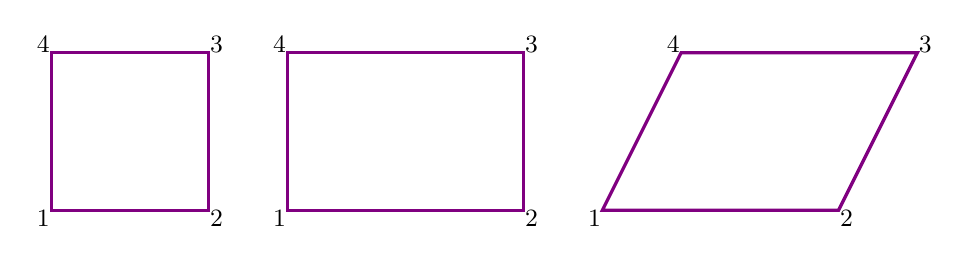
\begin{tikzpicture}
%\draw[fill=gray!23,gray!23](0,0) rectangle (13,4);
%\draw[step=0.5cm,gray,very thin] (0,0) grid (13,4); %background grid
\draw[very thick, violet] (1,1)--(3,1)--(3,3)--(1,3) --cycle ; %square
\node[] at (0.9,0.9) {\small $1$};
\node[] at (3.1,0.9) {\small $2$};
\node[] at (3.1,3.1) {\small $3$};
\node[] at (0.9,3.1) {\small $4$};
\draw[very thick, violet] (4,1)--(7,1)--(7,3)--(4,3) --cycle ; %rectangle
\node[] at (3.9,0.9) {\small $1$};
\node[] at (7.1,0.9) {\small $2$};
\node[] at (7.1,3.1) {\small $3$};
\node[] at (3.9,3.1) {\small $4$};
\draw[very thick, violet] (8,1)--(11,1)--(12,3)--(9,3) --cycle ; %parallelogram
\node[] at (7.9,0.9) {\small $1$};
\node[] at (11.1,0.9) {\small $2$};
\node[] at (12.1,3.1) {\small $3$};
\node[] at (8.9,3.1) {\small $4$};
\end{tikzpicture}
\end{center}

For the square of size $h$ we have 
\begin{eqnarray}
4A_2 &=& x_1 -x_2 +x_3 -x_4 = x_1 -(x_1+h) +(x_4+h) -x_4) =0 \nonumber\\
4A_4 &=& x_1 -x_2 +x_3 -x_4 = x_1 -(x_1+h) +(x_4+h) -x_4  =0 \nonumber\\
4B_2 &=& y_1 -y_2 +y_3 -y_4 = y_1 -y_2 + (y_2+h_y) -(y_1+h_y) = 0 \nonumber\\
4B_4 &=& y_1 -y_2 +y_3 -y_4 = y_1 -y_2 + (y_2+h_y) -(y_1+h_y) = 0 \nonumber
\end{eqnarray}
For the rectangle of size $h_x,h_y$ we have 
\begin{eqnarray}
4A_2 &=& x_1 -x_2 +x_3 -x_4 = x_1 -(x_1+h_x) +(x_4+h_x) -x_4) =0 \nonumber\\
4A_4 &=& x_1 -x_2 +x_3 -x_4 = x_1 -(x_1+h_x) +(x_4+h_x) -x_4  =0 \nonumber\\
4B_2 &=& y_1 -y_2 +y_3 -y_4 = y_1 -y_2 + (y_2+h_y) -(y_1+h_y) = 0 \nonumber\\
4B_4 &=& y_1 -y_2 +y_3 -y_4 = y_1 -y_2 + (y_2+h_y) -(y_1+h_y) = 0 \nonumber
\end{eqnarray}
and the same for the parallelogram.





In the case of a rectangle we also have
\begin{eqnarray}
A_1&=&\frac14(-x_1 +x_2 +x_3 -x_4)=\frac14(-x_1 +(x_1+h_x) +(x_4+h_x) -x_4) = \frac{h_x}{2} \nn\\
A_3&=&\frac14(-x_1 -x_2 +x_3 +x_4)=\frac14( -x_1 -(x_1+h_x) +(x_4+h_x) +x_4)  = 0 \nn\\
B_1 &=& \frac14 (-y_1 +y_2 +y_3 -y_4) = \frac14(-y_1 + y_2 + (y_2 +h_y) - (y_1+h_y)) = 0 \nn\\
B_3&=& \frac14(-y_1 -y_2 +y_3 +y_4) = \frac14 (-y_1 -y_2 + (y_2+h_y)+ (y_1+h_y)) = \frac{h_y}{2} \nn
\end{eqnarray}
and something very similar for the square with $h=h_x=h_y$.

For these quadrilaterals we then have
\[
{\bm J}^{-1} = \frac{1}{C}
\left(
\begin{array}{cc}
B_3  & -B_1  \\
-A_3  & A_1 
\end{array}
\right)
\qquad 
{\rm with }
\qquad
C= A_1B_3-A_3  B_1 
\]
and in the case of the rectangle:
\[
{\bm J} 
= \left(
\begin{array}{cc}
A_1  & B_1  \\
A_3  & B_3 
\end{array}
\right)
= \left(
\begin{array}{cc}
\frac{h_x}{2}  & 0  \\
0  & \frac{h_y}{2}
\end{array}
\right)
\]
The determinant is then $C=\frac{h_xh_y}{4}$ and the inverse:
\[
{\bm J}^{-1}
= 
\frac{1}{C}
\left(
\begin{array}{cc}
B_3  & -B_1  \\
-A_3  & A_1
\end{array}
\right)
= 
\frac{4}{h_xh_y}
\left(
\begin{array}{cc}
\frac{h_y}{2}  & 0  \\
0  & \frac{h_x}{2}
\end{array}
\right)
=
\left(
\begin{array}{cc}
\frac{2}{h_x}  & 0  \\
0  & \frac{2}{h_y}
\end{array}
\right)
\]


\begin{remark}
\textcite{hua90} (1990) has published analytical inverse transformation 
for quadrilateral isoparametric elements, i.e. how to compute ${\bm J}^{-1}$ 
as a function of space coordinates and not just at the quadrature points. 
\end{remark}


%==============================================================================
\section{Biquadratic mapping of a straight-edge face $Q_2$ element }

\begin{center}
\includegraphics[width=8cm]{images/mappings/biquadratic/mapping1}
\end{center}

The reference element now contains 9 nodes: 1,3,7,9 are the corners, nodes
2,4,6,8 are the mid-face points and node 5 is in the middle\footnote{Note that 
this numbering is quite arbitrary}.
The mapping from the $(r,s)$ space to the $(x,y)$ space is then as follows:

\begin{eqnarray}
\left(\begin{array}{c}
x(r,s) \\ y(r,s)
\end{array}\right)
=\sum_{i=1}^9 
\bN_i(r,s)\left(\begin{array}{c} x_i \\ y_i \end{array}\right)
&=&
\bN_1(r,s)\left(\begin{array}{c} x_1 \\ y_1 \end{array}\right)
+
\bN_2(r,s)\left(\begin{array}{c} x_2 \\ y_2 \end{array}\right)
+
\bN_3(r,s)\left(\begin{array}{c} x_3 \\ y_3 \end{array}\right)\nonumber\\
&+&
\bN_4(r,s)\left(\begin{array}{c} x_4 \\ y_4 \end{array}\right)
+
\bN_5(r,s)\left(\begin{array}{c} x_5 \\ y_5 \end{array}\right)
+
\bN_6(r,s)\left(\begin{array}{c} x_6 \\ y_6 \end{array}\right)\nonumber\\
&+&
\bN_7(r,s)\left(\begin{array}{c} x_7 \\ y_7 \end{array}\right)
+
\bN_8(r,s)\left(\begin{array}{c} x_8 \\ y_8 \end{array}\right) 
+
\bN_9(r,s)\left(\begin{array}{c} x_9 \\ y_9 \end{array}\right) \nonumber
\end{eqnarray}
where the $Q_2$ basis functions have been obtained in Section~\ref{ss:q22d}:
\begin{eqnarray}
\bN_1(r,t)&=& 0.5r(r-1)  0.5t(t-1) \nonumber\\
\bN_2(r,t)&=&      (1-r^2)  0.5t(t-1) \nonumber\\
\bN_3(r,t)&=& 0.5r(r+1)  0.5t(t-1) \nonumber\\
\bN_4(r,t)&=& 0.5r(r-1)       (1-t^2) \nonumber\\
\bN_5(r,t)&=&      (1-r^2)       (1-t^2) \nonumber\\
\bN_6(r,t)&=& 0.5r(r+1)       (1-t^2) \nonumber\\
\bN_7(r,t)&=& 0.5r(r-1)  0.5t(t+1) \nonumber\\
\bN_8(r,t)&=&      (1-r^2)  0.5t(t+1) \nonumber\\
\bN_9(r,t)&=& 0.5r(r+1)  0.5t(t+1) \nonumber
\end{eqnarray}

As in the previous section I have written a simple Python script that 
computes the image of 10,000 points generated in the reference element
using the forward mapping based on the $Q_2$ basis functions:
\begin{lstlisting}
x1=-1                 ; y1=-2
x3=3                  ; y3=-1
x9=2                  ; y9=2
x7=-3                 ; y7=1
x2=0.5*(x1+x3)        ; y2=0.5*(y1+y3)
x4=0.5*(x1+x7)        ; y4=0.5*(y1+y7)
x6=0.5*(x3+x9)        ; y6=0.5*(y3+y9)
x8=0.5*(x7+x9)        ; y8=0.5*(y7+y9)
x5=0.25*(x1+x3+x7+x9) ; y5=0.25*(y1+y3+y7+y9)

npts=10000
r=np.zeros(npts,dtype=np.float64)   
s=np.zeros(npts,dtype=np.float64)   
xQ1=np.zeros(npts,dtype=np.float64)   
yQ1=np.zeros(npts,dtype=np.float64)   
xQ2=np.zeros(npts,dtype=np.float64)   
yQ2=np.zeros(npts,dtype=np.float64)   

for i in range(0,npts):
    # compute random r,s coordinates
    r[i]=random.uniform(-1.,+1)
    s[i]=random.uniform(-1.,+1)
    # compute Q2 basis function values at r,s
    N1= 0.5*r[i]*(r[i]-1.) * 0.5*s[i]*(s[i]-1.)
    N2=       (1.-r[i]**2) * 0.5*s[i]*(s[i]-1.)
    N3= 0.5*r[i]*(r[i]+1.) * 0.5*s[i]*(s[i]-1.)
    N4= 0.5*r[i]*(r[i]-1.) *       (1.-s[i]**2)
    N5=       (1.-r[i]**2) *       (1.-s[i]**2)
    N6= 0.5*r[i]*(r[i]+1.) *       (1.-s[i]**2)
    N7= 0.5*r[i]*(r[i]-1.) * 0.5*s[i]*(s[i]+1.)
    N8=       (1.-r[i]**2) * 0.5*s[i]*(s[i]+1.)
    N9= 0.5*r[i]*(r[i]+1.) * 0.5*s[i]*(s[i]+1.)
    # compute x,y coordinates
    xQ2[i]=N1*x1+N2*x2+N3*x3+N4*x4+N5*x5+N6*x6+N7*x7+N8*x8+N9*x9
    yQ2[i]=N1*y1+N2*y2+N3*y3+N4*y4+N5*y5+N6*y6+N7*y7+N8*y8+N9*y9
    # compute Q1 basis function values at r,s
    N1=0.25*(1-r[i])*(1-s[i])
    N2=0.25*(1+r[i])*(1-s[i])
    N3=0.25*(1+r[i])*(1+s[i])
    N4=0.25*(1-r[i])*(1+s[i])
    # compute x,y coordinates
    xQ1[i]=N1*x1+N2*x3+N3*x9+N4*x7
    yQ1[i]=N1*y1+N2*y3+N3*y9+N4*y7

np.savetxt('rs.ascii',np.array([r,s]).T)
np.savetxt('xyQ1.ascii',np.array([xQ1,yQ1]).T)
np.savetxt('xyQ2.ascii',np.array([xQ2,yQ2]).T)
\end{lstlisting}

The code is available in {\tt /images/mappings/biquadratic}
Note that the coordinates of point 5 are defined being those of the 
average of the corner coordinates of the quadrilateral. More on this choice later.

\begin{center}
\includegraphics[width=5.7cm]{images/mappings/biquadratic/rs.pdf}
\includegraphics[width=5.7cm]{images/mappings/biquadratic/xyQ1.pdf}
\includegraphics[width=5.7cm]{images/mappings/biquadratic/xyQ2.pdf}\\
{\captionfont Left: 10,000 random points in the reference element; 
image of these points by means of a bilinear (middle) and biquadratic (right)
mapping respectively.}
\end{center}
When the sides of the element are straight we see that a $Q_1$ mapping is sufficient.

%.................................................................
\section{Biquadratic mapping of a not-so straight-line face $Q_2$ element }

We now carry out the same exercise as before but nodes 2 and 8 are no more 
in the middle of nodes 1-3 and 7-9 respectively.
The code is available in {\tt /images/mappings/biquadratic2}.

\begin{center}
\includegraphics[width=5.7cm]{images/mappings/biquadratic2/rs.pdf}
\includegraphics[width=5.7cm]{images/mappings/biquadratic2/xyQ1.pdf}
\includegraphics[width=5.7cm]{images/mappings/biquadratic2/xyQ2.pdf}\\
{\captionfont Left: 10,000 random points in the reference element; 
image of these points by means of a bilinear (middle) and biquadratic mapping 
respectively (right).} 
\end{center}

In this case we see that 
the $Q_2$ mapping manages to better capture the 'real' shape of the element.
Since nodes 2 and 8 have moved, we could now ask ourselves 
where we should place node 5? In this example we set it as follows
but it is somewhat arbitrary.
\begin{lstlisting}
x5=(x1+x2+x3+x4+x6+x7+x8+x9)/8. 
y5=(y1+y2+y3+y4+y6+y7+y8+y9)/8.
\end{lstlisting}
We will come back to this later.

%.......................................................................
\section{Bilinear, biquadratic and bicubic mapping in an annulus }

In the light of what precedes, we can now ask ourselves how this translates to 
a real geodynamic case. Let us then consider the case of an annular domain, 
a cross section of a hollow sphere. 
When using quadrilateral elements, the mesh will look similar to this:

\begin{center}
\includegraphics[width=6cm]{images/mappings/curved/annulus_mesh}
\end{center}

We here focus on $Q_1$, $Q_2$ and $Q_3$ mappings. We single out an element, 
and arbitrarily define it as follows in polar coordinates:
\begin{lstlisting}
theta1=23./180.*np.pi
theta2=52./180.*np.pi
R1=1.
R2=1.5
\end{lstlisting}
The $Q_1$ mapping requires four points, the $Q_2$ nine points and the $Q_3$
sixteen points. 
The code used in the following is available at {\tt ./images/mappings/curved/}.
These are placed equidistantly in the $r,\theta$ coordinate
system, as shown hereunder:

\begin{center}
\includegraphics[width=7cm]{images/mappings/curved/nodesQ1.pdf}
\includegraphics[width=7cm]{images/mappings/curved/nodesQ2.pdf}\\
\includegraphics[width=7cm]{images/mappings/curved/nodesQ3.pdf}
\includegraphics[width=7cm]{images/mappings/curved/nodesQ4.pdf}\\
{\captionfont Position of the nodes for the $Q_1$, $Q_2$, $Q_2$ and $Q_4$ mappings.}
\end{center}

As before, we randomly shoot 10,000 points inside the reference element 
and map these out in the $x,y$ space. Resulting swarms of points are shown 
in the following figures:

\begin{center}
\includegraphics[width=7cm]{images/mappings/curved/xy1_volume.pdf}
\includegraphics[width=7cm]{images/mappings/curved/xy2_volume.pdf}\\
\includegraphics[width=7cm]{images/mappings/curved/xy3_volume.pdf}
\includegraphics[width=7cm]{images/mappings/curved/xy3_volume.pdf}\\
{\captionfont Left to right: position of the mapped points for the $Q_1$, $Q_2$, $Q_3$ 
and $Q_4$ mappings.}
\end{center}

The image of a square with a $Q_1$ mapping is obviously a quadrilateral
so that it looks like quite a few points land outside of the domain $R_1\leq r\leq R_2$.
Note that points are well within $23\degree \leq \theta \leq 52\degree$, which can 
simply be explained by the fact that the faces of the element joining $R_1$
to $R_2$ are straight lines.

However, it looks like the biquadratic and bicubic mappings are doing a much better 
job at mapping the region of space $R_1\leq r\leq R_2$. In order to characterise 
this better, we now place 10,000 points on the bottom face of 
the reference element (i.e. $s=-1$)
and once again compute their coordinates in the the $x,y$ space:

\begin{center}
\includegraphics[width=8cm]{images/mappings/curved/xy1_line.pdf}
\includegraphics[width=8cm]{images/mappings/curved/xy2_line.pdf}\\
\includegraphics[width=8cm]{images/mappings/curved/xy3_line.pdf}
\includegraphics[width=8cm]{images/mappings/curved/xy4_line.pdf}\\
{\captionfont Position of the mapped points for the $Q_1$, $Q_2$, $Q_3$ and $Q_4$ mappings.}
\end{center}

For each point $i$ we now compute the distance $r_i$ 
to the origin, which, if the 
mapping was perfect, would be exactly equal to $R_1=1$. 
On the following plots are shown the error $r_i-1$ for all 
points, from $r=-1$ to $r=+1$.

\begin{center}
\includegraphics[width=8cm]{images/mappings/curved/innerline_error_Q1mapping.pdf}
\includegraphics[width=8cm]{images/mappings/curved/innerline_error_Q2mapping.pdf}\\
\includegraphics[width=8cm]{images/mappings/curved/innerline_error_Q3mapping.pdf}
\includegraphics[width=8cm]{images/mappings/curved/innerline_error_Q4mapping.pdf}\\
{\captionfont Radius error of the mapped points for the $Q_1$, $Q_2$, $Q_3$ and $Q_4$ mappings.}
\end{center}

We see that the amplitude of the error decreases with the order of the mapping used, 
which is why for instance \aspect uses a $Q_4$ mapping by default\footnote{I find it also quite striking 
that the $Q_4$ mapping outperforms the $Q_3$ one by two orders of magnitude...}.
Actually, in this particular case, the equation which describes the circle is not a 
polynomial so that no high-order mapping will ever be able to {\it exactly} 
represent the curved boundary of the element!

Another interesting point to keep in mind is that the location of the quadrature points
in the $x,y$ space is also determined by the mapping used, which can have consequences
on the accuracy of the integration and it will be reflected (for instance) on the 
error convergence rate.

As already mentioned previously, 
the coordinates of the nodes of the element in the $x,y$ are 
uniquely determined when they are on the convex hull of the element (
for instance nodes 0-7 for $Q_2$) but we need to choose the position 
of the last nodes which are inside the element. Unfortunately, this choice is 
not neutral. 

Finally, we can explore the importance of the mapping in combination with 
numerical quadrature. For each mapping we compute the area of the element
by means of a 3x3, 4x4 or 5x5 quadrature.

\begin{verbatim}
**********Q1*********
nqperdim= 3 0.3030060126539606 rel. error -0.04215361698430029
nqperdim= 4 0.3030060126539606 rel. error -0.04215361698430012 ~ 4%
nqperdim= 5 0.3030060126539606 rel. error -0.04215361698430012
**********Q2*********
nqperdim= 3 0.3162980025394154 rel. error -0.00013569026611326453
nqperdim= 4 0.3162980025394155 rel. error -0.00013569026611308905 ~ 0.01%
nqperdim= 5 0.3162980025394154 rel. error -0.00013569026611326453
**********Q3*********
nqperdim= 3 0.3163472223929359 rel. error 1.9900899402587318e-05
nqperdim= 4 0.316347222392936  rel. error 1.9900899402938278e-05 ~ 0.002%
nqperdim= 5 0.316347222392936  rel. error 1.9900899402938278e-05
**********Q4*********
nqperdim= 3 0.3163409410866220 rel. error 4.477021014282521e-08
nqperdim= 4 0.3163409541901677 rel. error 8.619243716974044e-08 ~ 0.000008%
nqperdim= 5 0.316340954190168  rel. error 8.619243804713484e-08
\end{verbatim}

Here again the $Q_4$ mapping makes quite the difference. 

\newpage

%..................................................................
\section{Biquadratic mapping - the middle node conundrum}

Python code at {\tt images/mappings/biquadratic3}.

As mentioned before, unless the element is a straight-edge quadrilateral, 
determining the (best) position of the middle node is not trivial. Or is it?

Let us recall the internal numbering of nodes:
\begin{verbatim}
4--7--3
|     |
8  9  6   (reference element)
|     |
1--5--2
\end{verbatim}


We can think of multiple ways to come up with the `center' of the element, 
i.e. the location of node \#9. %this point that we denote by $I$.
In the code these different approaches are parameterized by means of the
\lstinline{center} variable:

\begin{itemize}
\item \lstinline{center=0}: The middle node coordinates are simply the 
average of the corner coordinates 
\begin{align}
x_9&=(x_1+x_2+x_3+x_4)/4 \nn\\
y_9&=(y_1+y_2+y_3+y_4)/4 \nn
\end{align}

\item \lstinline{center=1}: The middle coordinates are the average all the 
4 corners and 4 mid-edge nodes coordinates:

\begin{align}
x_9&=(x_1+x_2+x_3+x_4+x_5+x_6+x_7+x_8)/8 \nn\\
y_9&=(y_1+y_2+y_3+y_4+y_5+y_6+y_7+y_8)/8 \nn
\end{align}

\item \lstinline{center=2}: The middle coordinates are obtained via a 
weighed sum of the corner coordinates and the mid-edge nodes 
coordinates\footnote{I have no idea where this comes from.}: 

\begin{align}
x_9&=(x_1+x_2+x_3+x_4+3x_5+3x_6+3x_7+3x_8)/16. \nn\\
y_9&=(y_1+y_2+y_3+y_4+3y_5+3y_6+3y_7+3y_8)/16. \nn
\end{align}

\item \lstinline{center=3}: This only applies to element \#4 that is defined on an annulus:

\begin{align}
x_9&=\frac12(R_1+R_2)\cos(3\pi/8) \nn\\
y_9&=\frac12(R_1+R_2)\sin(3\pi/8) \nn
\end{align}


\item \lstinline{center=4}: This only applies to element \#4 that is 
defined by $R_1<r<R_2$ and $\theta_1<\theta<\theta_2$. Node \#9 is the center of mass. 

\todo[inline]{other elements}

We need to compute\footnote{\url{https://en.wikipedia.org/wiki/Center_of_mass}}
\begin{eqnarray}
\vec{R} 
&=&\frac{1}{M} \int \vec{r} \rho(\vec r) dV \nn\\
&=&\frac{1}{M} \rho_0 \int \vec{r} dV\nn\\
&=&\frac{1}{M} \frac{M}{V} \int \vec{r} dV\nn\\
&=&\frac{1}{V} \int \vec{r} dV\nn\\
&=&\frac{1}{V} \int \left(\begin{array}{c} x \\ y \end{array}\right)  dV\nn\\
&=&\frac{1}{V} \int \left(\begin{array}{c} r \cos \theta \\ r \sin\theta \end{array}\right)dV\nn\\
&=&\frac{1}{V} \int_{R_1}^{R_2} \int_{\theta_1}^{\theta_2} \left(\begin{array}{c} r \cos \theta 
\\ r \sin\theta \end{array}\right)  r dr d\theta\nn\\
&=&\frac{1}{\frac12 (R_2^2-R_1^2) (\theta_2-\theta_1)} \frac13(R_2^3-R_1^3) 
\left(
\begin{array}{c}
\sin\theta_2-\sin\theta_1 \\
-\cos\theta_2+\cos\theta_1 
\end{array}
\right) \nn\\
&\simeq& 
\left(
\begin{array}{c}
0.5801028000103104\\
1.4004920473554983
\end{array}
\right) 
\end{eqnarray}
which corresponds to $r=1.5158816686291174$ and $\theta=67.5^o=3\pi/8$.

\item \lstinline{center=5}: variable position

\item \lstinline{center=6}: This approach is a bit more complex than the previous ones.
We start by acknowledging that we know the coordinates of nodes 1-8 in the reference space $(r,s)$ 
and in the real space $(x,y)$ so one could then use a $Q_2^{(8)}$ mapping (i.e. 'serendipity' $Q_2$)
to place node \#9.

In this case the basis functions for this mapping are defined in Section~\ref{sec:serendipity2D}:
\begin{eqnarray}
\bN_0(r,s)&=& \frac{1}{4}(1-r)(1-s)(-r-s-1) \nn\\
\bN_1(r,s)&=& \frac{1}{4}(1+r)(1-s)(r-s-1) \nn\\
\bN_2(r,s)&=& \frac{1}{4}(1+r)(1+s)(r+s-1) \nn\\
\bN_3(r,s)&=& \frac{1}{4}(1-r)(1+s)(-r+s-1) \nn\\
\bN_4(r,s)&=& \frac{1}{2}(1-r^2)(1-s)  \nn\\
\bN_5(r,s)&=& \frac{1}{2}(1+r)  (1-s^2)\nn\\
\bN_6(r,s)&=& \frac{1}{2}(1-r^2)(1+s)  \nn\\
\bN_7(r,s)&=& \frac{1}{2}(1-r)  (1-s^2) \nn
\end{eqnarray}

We would then compute the location of node 9 as follows (its $r,s$ coordinates are $0,0$): 
\begin{eqnarray}
x_9 
&=& \sum_{i=1}^8 \bN_i (r_9,s_9) x_i \nn\\
&=& \sum_{i=1}^8 \bN_i (0,0) x_i \nn\\
&=& -\frac14 (x_1+x_2+x_3+x_4) + \frac12 (x_5+x_6+x_7+x_8) \nn\\
y_9 
&=& \sum_{i=1}^8 \bN_i (r_9,s_9) y_i \nn\\
&=& \sum_{i=1}^8 \bN_i (0,0) y_i \nn\\
&=& -\frac14 (y_1+y_2+y_3+y_4) + \frac12 (y_5+y_6+y_7+y_8) \nn
\end{eqnarray}


\end{itemize}

%...............................
\subsection*{About the code}

In all what follows we use a $Q_2$ isoparametric mapping.

For simplicity I use in what follows the function $f(x,y)=x^3+y^3$.
At each point $(r,s)\in [-1,1]^2$ with real coordinates ($x(r,s),y(r,s)$) 
we compute the error $e_f=\sum_i \bN_i(r,s) f_i  - f(xi(r,s),y(r,s))$ 
where $f_i$ are the values of the function evaluated at the 9 nodes.
We also compute the error on the first order derivatives, i.e.
$e_{df/dx}=\sum_i \bN_i(r,s) (df/dx)_i  - df/dx(x(r,s),y(r,s))$ 
and $e_{df/dy}=\sum_i \bN_i(r,s) (df/dy)_i  - df/dy(x(r,s),y(r,s))$.

Unless indicated otherwise $3 \times 3$ quadrature is used to a) compute
the area of the element; b) compute the errors above in the $L_2$ norm,
e.g. $E_f=\left(\int_\Omega (e_f)^2 dV \right)^{1/2}$ (I purposefully do not 
divide by the area) and $E_{\nabla f}=\left(\int_\Omega (e_{df/dx}^2+e_{df/dy}^2) dV \right)^{1/2}$.

We find that for all element shapes the measured area seems to be independent 
of the position of middle node. Why?

We note that the position of edges obtained from the 
forward mapping by setting $r=\pm 1$ and/or $s=\pm 1$ are in fact
independent of the position of the middle node since shape functions are zero there.
For example, setting $s=-1$ means that for terms containing 
this summation $\sum_i \bN_i(r,s) ...$  only contributions by nodes
1,5,2 count (basis functions $\bN_{3,4,6,7,8,9}$ are zero for $s=-1$).
When computing $y=\sum_i \bN_i(r,s=-1) y_i$ then the result is 
independent of $y_9$. Same for all sides.
 
\vspace{.5cm}

The Python code is built as follows:
\begin{verbatim}
for center in centers:
    assign middle point coordinates
    generate npts points at random in reference cell
    compute error on f,df/dx,df/dy and jacobian at each point
    export points and their fields to vtu
    compute area and integral of errors over element
\end{verbatim}

Warning: Note that all the conclusions drawn hereafter are provisory:
only *one* function was used which is arbitrarily chosen to be a 3rd order polynomial,
and the coordinates/shapes of the elements 1,2,3 are also arbitrary and results
may differ with different configurations!



\newpage
%------------------------------------------------------------------------------
\subsection*{Element 0}
\begin{center}
\includegraphics[width=3.5cm]{images/mappings/biquadratic3/elt0/element0}
\includegraphics[width=4cm]{images/mappings/biquadratic3/elt0/nodes}
\includegraphics[width=4cm]{images/mappings/biquadratic3/elt0/nodes_zoom}
\includegraphics[width=4cm]{images/mappings/biquadratic3/elt0/quad_points}\\
{\captionfont From left to right: element and its 8 boundary nodes.
Location of the 9 nodes for different values of the center parameter.
Zoom on the middle node. 
Position of the quadrature points for different values of the center parameter.}
\end{center}
\begin{lstlisting}
   x1=-1              ; y1=-1
   x2=1               ; y2=-1
   x3=1               ; y3=1
   x4=-1              ; y4=1
   x5=0.5*(x1+x2)     ; y5=0.5*(y1+y2)
   x6=0.5*(x2+x3)     ; y6=0.5*(y2+y3)
   x7=0.5*(x3+x4)     ; y7=0.5*(y3+y4)
   x8=0.5*(x1+x4)     ; y8=0.5*(y1+y4)
\end{lstlisting}

In this case all only {\python center=0,1,2,4,6} are applicable but they all 
lead to the same middle point with $x_9=0,y_9=0$. This means that the position of 
quadrature points is also independent of the {\python center} parameter.

\begin{tiny}
\begin{verbatim}
element= 0, npts= 1000000, nqperdim= 3
============================================================
center= 0 x9,y9= 0.000000e+00 0.000000e+00 
center= 0 min/max/avrg jcob on pts   = 1.000000e+00 1.000000e+00 1.000000e+00
center= 0 min/max/avrg err_f on pts   = -7.697997e-01 7.697981e-01 1.032961e-04
center= 0 min/max/avrg err_dfdx on pts= -1.999994e+00 1.000000e+00 9.897925e-04
center= 0 min/max/avrg err_dfdy on pts= -1.999998e+00 1.000000e+00 -4.337008e-04
center= 0 int err_f= 6.531973e-01
center= 0 int err_gradf= 2.529822e+00
center= 0 area= 4.000000e+00
============================================================
center= 1 x9,y9= 0.000000e+00 0.000000e+00 
center= 1 min/max/avrg jcob on pts   = 1.000000e+00 1.000000e+00 1.000000e+00
center= 1 min/max/avrg err_f on pts   = -7.697981e-01 7.697978e-01 -1.037079e-04
center= 1 min/max/avrg err_dfdx on pts= -1.999994e+00 1.000000e+00 5.562081e-04
center= 1 min/max/avrg err_dfdy on pts= -1.999992e+00 1.000000e+00 -6.057413e-04
center= 1 int err_f= 6.531973e-01
center= 1 int err_gradf= 2.529822e+00
center= 1 area= 4.000000e+00
============================================================
center= 2 x9,y9= 0.000000e+00 0.000000e+00 
center= 2 min/max/avrg jcob on pts   = 1.000000e+00 1.000000e+00 1.000000e+00
center= 2 min/max/avrg err_f on pts   = -7.698001e-01 7.697999e-01 -4.504134e-04
center= 2 min/max/avrg err_dfdx on pts= -1.999985e+00 1.000000e+00 4.678516e-04
center= 2 min/max/avrg err_dfdy on pts= -1.999987e+00 1.000000e+00 1.466204e-03
center= 2 int err_f= 6.531973e-01
center= 2 int err_gradf= 2.529822e+00
center= 2 area= 4.000000e+00
============================================================
center= 6 x9,y9= 0.000000e+00 0.000000e+00 
center= 6 min/max/avrg jcob on pts   = 1.000000e+00 1.000000e+00 1.000000e+00
center= 6 min/max/avrg err_f on pts   = -7.697964e-01 7.698001e-01 -3.862548e-04
center= 6 min/max/avrg err_dfdx on pts= -1.999996e+00 1.000000e+00 -3.443542e-04
center= 6 min/max/avrg err_dfdy on pts= -1.999992e+00 1.000000e+00 -9.219252e-04
center= 6 int err_f= 6.531973e-01
center= 6 int err_gradf= 2.529822e+00
center= 6 area= 4.000000e+00
============================================================
\end{verbatim}
\end{tiny}

We find that the jacobian is exactly 1 everywhere in the element which 
is what we expected since $|J|=4/h_xh_y=4/2\cdot 2=1$.
Likewise area measurements are all identical and equal to $h_xh_y$.

Conclusions:
\begin{itemize}
\item In the case of square/rectangular elements the middle node
location is indeed 'in the middle'.
\item we obviously recover the same values for $e_f$ and $E_{\nabla f}$
\item Even using 1,000,000 points we find that the min/max/avrg values
of pointwise errors show significant differences (esp. the average). 
In the future we'll then only consider $E$ errors. 
\end{itemize}


%\begin{center}
%\includegraphics[width=5.7cm]{images/mappings/biquadratic3/elt0/jcob}
%{\captionfont 10,000 points at random.} 
%\end{center}


\newpage
%------------------------------------------------------------------------------
\subsection*{Element 1}
\begin{center}
\includegraphics[width=3.5cm]{images/mappings/biquadratic3/elt1/element1}
\includegraphics[width=4cm]{images/mappings/biquadratic3/elt1/nodes}
\includegraphics[width=4cm]{images/mappings/biquadratic3/elt1/nodes_zoom}
\includegraphics[width=4cm]{images/mappings/biquadratic3/elt1/quad_points}
\end{center}
\begin{lstlisting}
   x1=-1              ; y1=-2
   x2=3               ; y2=-1
   x3=2               ; y3=2
   x4=-3              ; y4=1
   x5=0.5*(x1+x2)     ; y5=0.5*(y1+y2)
   x6=0.5*(x2+x3)     ; y6=0.5*(y2+y3)
   x7=0.5*(x3+x4)     ; y7=0.5*(y3+y4)
   x8=0.5*(x1+x4)     ; y8=0.5*(y1+y4)
\end{lstlisting}

In this case only {\python center=0,1,2,4,6} are applicable but they all 
lead to the same middle point with $x_9=0,y_9=0$. This means that the position of 
quadrature points is also independent of the {\python center} parameter.

\begin{tiny}
\begin{verbatim}
element= 1, npts= 1000000, nqperdim= 3
============================================================
center= 0 x9,y9= 2.500000e-01 0.000000e+00 
center= 0 min/max/avrg jcob on pts   = 3.250362e+00 4.249199e+00 3.750057e+00
center= 0 min/max/avrg err_f on pts   = -6.060741e+00 6.666524e+00 1.688878e-03
center= 0 min/max/avrg err_dfdx on pts= -1.099651e+01 6.443612e+00 -5.010148e-03
center= 0 min/max/avrg err_dfdy on pts= -1.015984e+01 4.225070e+00 1.686068e-02
center= 0 int err_f= 1.107770e+01
center= 0 int err_gradf= 1.954635e+01
center= 0 area= 1.500000e+01
============================================================
center= 1 x9,y9= 2.500000e-01 0.000000e+00 
center= 1 min/max/avrg jcob on pts   = 3.250930e+00 4.249578e+00 3.749771e+00
center= 1 min/max/avrg err_f on pts   = -6.060172e+00 6.666509e+00 -4.038311e-03
center= 1 min/max/avrg err_dfdx on pts= -1.099842e+01 6.444102e+00 -1.172403e-04
center= 1 min/max/avrg err_dfdy on pts= -1.018956e+01 4.225064e+00 1.654201e-02
center= 1 int err_f= 1.107770e+01
center= 1 int err_gradf= 1.954635e+01
center= 1 area= 1.500000e+01
============================================================
center= 2 x9,y9= 2.500000e-01 0.000000e+00 
center= 2 min/max/avrg jcob on pts   = 3.251054e+00 4.249622e+00 3.750130e+00
center= 2 min/max/avrg err_f on pts   = -6.060921e+00 6.666524e+00 -6.843429e-03
center= 2 min/max/avrg err_dfdx on pts= -1.099522e+01 6.441666e+00 -3.864851e-03
center= 2 min/max/avrg err_dfdy on pts= -1.018380e+01 4.225069e+00 1.319091e-02
center= 2 int err_f= 1.107770e+01
center= 2 int err_gradf= 1.954635e+01
center= 2 area= 1.500000e+01
============================================================
center= 6 x9,y9= 2.500000e-01 0.000000e+00 
center= 6 min/max/avrg jcob on pts   = 3.250841e+00 4.249203e+00 3.749670e+00
center= 6 min/max/avrg err_f on pts   = -6.060064e+00 6.666475e+00 -9.101238e-04
center= 6 min/max/avrg err_dfdx on pts= -1.099351e+01 6.443416e+00 -7.271667e-03
center= 6 min/max/avrg err_dfdy on pts= -1.016288e+01 4.225062e+00 1.436911e-02
center= 6 int err_f= 1.107770e+01
center= 6 int err_gradf= 1.954635e+01
center= 6 area= 1.500000e+01
============================================================
\end{verbatim}
\end{tiny}
 
%\begin{center}
%\includegraphics[width=5.7cm]{images/mappings/biquadratic3/elt1/jcob}
%{\captionfont 10,000 points at random.} 
%\end{center}


Conclusions:
\begin{itemize}
\item Exactly the same conclusions as for element 0 can be drawn.
\end{itemize} 




\newpage
%------------------------------------------------------------------------------
\subsection*{Element 2}
\begin{center}
\includegraphics[width=3.5cm]{images/mappings/biquadratic3/elt2/element2}
\includegraphics[width=4cm]{images/mappings/biquadratic3/elt2/nodes}
\includegraphics[width=4cm]{images/mappings/biquadratic3/elt2/nodes_zoom}
\includegraphics[width=4cm]{images/mappings/biquadratic3/elt2/quad_points}
\end{center}
\begin{lstlisting}
   x1=-1 ; y1=-2
   x2=3  ; y2=-1
   x3=2  ; y3=2
   x4=-3 ; y4=1
   x5=0.5*(x1+x2) ; y5=0.5*(y1+y2) -0.25
   x6=0.5*(x2+x3) ; y6=0.5*(y2+y3)
   x7=0.5*(x3+x4) ; y7=0.5*(y3+y4) +0.5
   x8=0.5*(x1+x4) ; y8=0.5*(y1+y4)
\end{lstlisting}

\begin{tiny}
\begin{verbatim}
element= 2, npts= 1000000, nqperdim= 3
============================================================
center= 0 x9,y9= 2.500000e-01 0.000000e+00 
center= 0 min/max/avrg jcob on pts   = 3.003425e+00 5.833227e+00 4.332919e+00
center= 0 min/max/avrg err_f on pts   = -5.308564e+00 7.373735e+00 1.289018e-01
center= 0 min/max/avrg err_dfdx on pts= -1.323435e+01 6.260039e+00 -3.403394e-02
center= 0 min/max/avrg err_dfdy on pts= -8.721839e+00 5.063460e+00 -6.697600e-02
center= 0 int err_f= 1.183453e+01
center= 0 int err_gradf= 2.148351e+01
center= 0 area= 1.733333e+01
============================================================
center= 1 x9,y9= 2.500000e-01 3.125000e-02 
center= 1 min/max/avrg jcob on pts   = 3.002755e+00 5.696725e+00 4.333505e+00
center= 1 min/max/avrg err_f on pts   = -5.363672e+00 7.293081e+00 9.018116e-02
center= 1 min/max/avrg err_dfdx on pts= -1.323652e+01 6.221262e+00 -2.293697e-02
center= 1 min/max/avrg err_dfdy on pts= -8.682711e+00 5.047551e+00 -6.391543e-02
center= 1 int err_f= 1.178018e+01
center= 1 int err_gradf= 2.141089e+01
center= 1 area= 1.733333e+01
============================================================
center= 2 x9,y9= 2.500000e-01 4.687500e-02 
center= 2 min/max/avrg jcob on pts   = 3.002800e+00 5.630556e+00 4.332764e+00
center= 2 min/max/avrg err_f on pts   = -5.390923e+00 7.252336e+00 7.759085e-02
center= 2 min/max/avrg err_dfdx on pts= -1.321750e+01 6.199422e+00 -2.474020e-02
center= 2 min/max/avrg err_dfdy on pts= -8.715040e+00 5.038157e+00 -6.434275e-02
center= 2 int err_f= 1.175495e+01
center= 2 int err_gradf= 2.137246e+01
center= 2 area= 1.733333e+01
============================================================
center= 6 x9,y9= 2.500000e-01 1.250000e-01 
center= 6 min/max/avrg jcob on pts   = 3.003258e+00 5.340770e+00 4.332317e+00
center= 6 min/max/avrg err_f on pts   = -5.523826e+00 7.044686e+00 1.150397e-02
center= 6 min/max/avrg err_dfdx on pts= -1.321437e+01 6.083445e+00 -9.511932e-03
center= 6 min/max/avrg err_dfdy on pts= -8.679190e+00 4.976683e+00 -5.669887e-02
center= 6 int err_f= 1.164859e+01
center= 6 int err_gradf= 2.115913e+01
center= 6 area= 1.733333e+01
============================================================
\end{verbatim}
\end{tiny}

%\includegraphics[width=5.7cm]{images/mappings/biquadratic3/elt2/jcob_1}
%\includegraphics[width=5.7cm]{images/mappings/biquadratic3/elt2/jcob_2}\\
%{\captionfont 50,000 points at random. From left to right: center=0,1,2.} 
%\end{center}


Conclusions:
\begin{itemize}
\item the four approaches yield 4 different locations for the center.
\item $E_f$ very comparable across all four cases. center=6 seems to be the best
\item Same conclusion $E_{\nabla f}$ 
\end{itemize} 

\newpage
%------------------------------------------------------------------------------
\subsection*{Element 3}
\begin{center}
\includegraphics[width=3.5cm]{images/mappings/biquadratic3/elt3/element3}
\includegraphics[width=4cm]{images/mappings/biquadratic3/elt3/nodes}
\includegraphics[width=4cm]{images/mappings/biquadratic3/elt3/nodes_zoom}
\includegraphics[width=4cm]{images/mappings/biquadratic3/elt3/quad_points}
\end{center}
\begin{lstlisting}
   x1=-1 ; y1=-2
   x2=3  ; y2=-1
   x3=2  ; y3=2
   x4=-3 ; y4=1
   x5=0.5*(x1+x2)     ; y5=0.5*(y1+y2) -0.5
   x6=0.5*(x2+x3)+0.4 ; y6=0.5*(y2+y3) +0.1
   x7=0.5*(x3+x4)     ; y7=0.5*(y3+y4) +0.5
   x8=0.5*(x1+x4)-0.2 ; y8=0.5*(y1+y4) -0.1
\end{lstlisting}

\begin{tiny}
\begin{verbatim}
element= 3, npts= 1000000, nqperdim= 3
============================================================
center= 0 x9,y9= 2.500000e-01 0.000000e+00 
center= 0 min/max/avrg jcob on pts   = 1.907940e+00 5.649991e+00 4.849153e+00
center= 0 min/max/avrg err_f on pts   = -7.275654e+00 9.566299e+00 1.918971e-01
center= 0 min/max/avrg err_dfdx on pts= -1.653858e+01 6.294598e+00 -2.527334e-01
center= 0 min/max/avrg err_dfdy on pts= -2.581218e+01 5.947161e+00 -3.542729e-01
center= 0 int err_f= 1.614533e+01
center= 0 int err_gradf= 2.925334e+01
center= 0 area= 1.940000e+01
============================================================
center= 1 x9,y9= 2.750000e-01 1.387779e-17 
center= 1 min/max/avrg jcob on pts   = 1.903598e+00 5.677286e+00 4.850195e+00
center= 1 min/max/avrg err_f on pts   = -7.297901e+00 9.493156e+00 1.465801e-01
center= 1 min/max/avrg err_dfdx on pts= -1.657761e+01 6.261874e+00 -2.442038e-01
center= 1 min/max/avrg err_dfdy on pts= -2.587333e+01 5.949630e+00 -3.426886e-01
center= 1 int err_f= 1.605547e+01
center= 1 int err_gradf= 2.915732e+01
center= 1 area= 1.940000e+01
============================================================
center= 2 x9,y9= 2.875000e-01 0.000000e+00 
center= 2 min/max/avrg jcob on pts   = 1.904405e+00 5.693478e+00 4.849918e+00
center= 2 min/max/avrg err_f on pts   = -7.308703e+00 9.456916e+00 1.279976e-01
center= 2 min/max/avrg err_dfdx on pts= -1.668960e+01 6.246507e+00 -2.416973e-01
center= 2 min/max/avrg err_dfdy on pts= -2.604266e+01 5.951170e+00 -3.517167e-01
center= 2 int err_f= 1.601397e+01
center= 2 int err_gradf= 2.910870e+01
center= 2 area= 1.940000e+01
============================================================
center= 6 x9,y9= 3.500000e-01 5.551115e-17 
center= 6 min/max/avrg jcob on pts   = 1.913670e+00 5.787307e+00 4.849397e+00
center= 6 min/max/avrg err_f on pts   = -7.359196e+00 9.279116e+00 1.625764e-02
center= 6 min/max/avrg err_dfdx on pts= -1.661175e+01 6.169925e+00 -2.370181e-01
center= 6 min/max/avrg err_dfdy on pts= -2.588039e+01 5.961927e+00 -3.386132e-01
center= 6 int err_f= 1.584097e+01
center= 6 int err_gradf= 2.885993e+01
center= 6 area= 1.940000e+01
============================================================
\end{verbatim}
\end{tiny}

\newpage
\begin{center}
\includegraphics[width=4cm]{images/mappings/biquadratic3/elt3/jcob.0000.png}
\includegraphics[width=4cm]{images/mappings/biquadratic3/elt3/f.0000.png}
\includegraphics[width=4cm]{images/mappings/biquadratic3/elt3/dfdx.0000.png}
\includegraphics[width=4cm]{images/mappings/biquadratic3/elt3/dfdy.0000.png}\\
\includegraphics[width=4cm]{images/mappings/biquadratic3/elt3/jcob.0001.png}
\includegraphics[width=4cm]{images/mappings/biquadratic3/elt3/f.0001.png}
\includegraphics[width=4cm]{images/mappings/biquadratic3/elt3/dfdx.0001.png}
\includegraphics[width=4cm]{images/mappings/biquadratic3/elt3/dfdy.0001.png}\\
\includegraphics[width=4cm]{images/mappings/biquadratic3/elt3/jcob.0002.png}
\includegraphics[width=4cm]{images/mappings/biquadratic3/elt3/f.0002.png}
\includegraphics[width=4cm]{images/mappings/biquadratic3/elt3/dfdx.0002.png}
\includegraphics[width=4cm]{images/mappings/biquadratic3/elt3/dfdy.0002.png}\\
\includegraphics[width=4cm]{images/mappings/biquadratic3/elt3/jcob.0003.png}
\includegraphics[width=4cm]{images/mappings/biquadratic3/elt3/f.0003.png}
\includegraphics[width=4cm]{images/mappings/biquadratic3/elt3/dfdx.0003.png}
\includegraphics[width=4cm]{images/mappings/biquadratic3/elt3/dfdy.0003.png}\\
{\captionfont 100,000 points at random. From left to right: jacobian, 
error on $f$, error on $df/dx$ and error on $df/dy$. From top
to bottom: center=0,1,2,6.} 
\end{center}


Conclusions:
\begin{itemize}
\item the four approaches yield 4 different locations for the center.
\item $E_f$ very comparable across all four cases. center=6 seems to be the best
\item Same conclusion $E_{\nabla f}$ 
\end{itemize} 

\begin{center}
\includegraphics[width=7cm]{images/mappings/biquadratic3/elt3/edges}\\
{\captionfont edges obtained by forward $Q_2$ mapping of points $r,s=\pm1$}
\end{center}





\newpage
%------------------------------------------------------------------------------
\subsection*{Element 4}

\begin{center}
\includegraphics[width=3.5cm]{images/mappings/biquadratic3/elt4/element4}
\includegraphics[width=4cm]{images/mappings/biquadratic3/elt4/nodes}
\includegraphics[width=4cm]{images/mappings/biquadratic3/elt4/nodes_zoom}
\includegraphics[width=4cm]{images/mappings/biquadratic3/elt4/quad_points}
\end{center}

\begin{lstlisting}
   R1=1
   R2=2
   dtheta=np.pi/4
   x1=R1*np.cos(np.pi/2-0)               ; y1=R1*np.sin(np.pi/2-0) 
   x5=R1*np.cos(np.pi/2-dtheta/2)        ; y5=R1*np.sin(np.pi/2-dtheta/2) 
   x2=R1*np.cos(np.pi/2-dtheta)          ; y2=R1*np.sin(np.pi/2-dtheta) 
   x8=0.5*(R1+R2)*np.cos(np.pi/2-0)      ; y8=0.5*(R1+R2)*np.sin(np.pi/2-0)  
   x6=0.5*(R1+R2)*np.cos(np.pi/2-dtheta) ; y6=0.5*(R1+R2)*np.sin(np.pi/2-dtheta) 
   x4=R2*np.cos(np.pi/2-0)               ; y4=R2*np.sin(np.pi/2-0)   
   x7=R2*np.cos(np.pi/2-dtheta/2)        ; y7=R2*np.sin(np.pi/2-dtheta/2)   
   x3=R2*np.cos(np.pi/2-dtheta)          ; y3=R2*np.sin(np.pi/2-dtheta)   
\end{lstlisting}



\begin{tiny}
\begin{verbatim}
center of mass coords (x,y): 0.5801028000103104 1.4004920473554983
center of mass coords (r,theta) 1.5158816686291174 67.5
element= 4
npts= 1000000
nqperdim= 3
============================================================
center= 0 x9,y9= 5.303301e-01 1.280330e+00 
center= 0 min/max/avrg jcob on pts   = 1.039732e-01 5.574373e-01 2.943883e-01
center= 0 min/max/avrg err_f on pts   = -2.262961e-01 3.113327e-01 9.571182e-03
center= 0 min/max/avrg err_dfdx on pts= -1.424648e+00 6.317490e-01 7.838307e-03
center= 0 min/max/avrg err_dfdy on pts= -2.934500e+00 1.004204e+00 -2.939049e-02
center= 0 int err_f= 1.333177e-01
center= 0 int err_gradf= 9.290509e-01
center= 0 area= 1.177180e+00
============================================================
center= 1 x9,y9= 5.412539e-01 1.306702e+00 
center= 1 min/max/avrg jcob on pts   = 1.258064e-01 5.136716e-01 2.941058e-01
center= 1 min/max/avrg err_f on pts   = -2.260227e-01 2.814548e-01 5.370194e-03
center= 1 min/max/avrg err_dfdx on pts= -1.425092e+00 6.022714e-01 1.754560e-02
center= 1 min/max/avrg err_dfdy on pts= -2.052857e+00 9.324228e-01 -1.974217e-02
center= 1 int err_f= 1.151357e-01
center= 1 int err_gradf= 8.033761e-01
center= 1 area= 1.177180e+00
============================================================
center= 2 x9,y9= 5.467157e-01 1.319889e+00 
center= 2 min/max/avrg jcob on pts   = 1.367421e-01 4.919188e-01 2.944290e-01
center= 2 min/max/avrg err_f on pts   = -2.261415e-01 2.680915e-01 3.934531e-03
center= 2 min/max/avrg err_dfdx on pts= -1.426224e+00 5.884028e-01 2.200854e-02
center= 2 min/max/avrg err_dfdy on pts= -1.715733e+00 9.007872e-01 -1.831880e-02
center= 2 int err_f= 1.074743e-01
center= 2 int err_gradf= 7.456708e-01
center= 2 area= 1.177180e+00
============================================================
center= 3 x9,y9= 5.740251e-01 1.385819e+00 
center= 3 min/max/avrg jcob on pts   = 1.913594e-01 4.118053e-01 2.942541e-01
center= 3 min/max/avrg err_f on pts   = -2.264001e-01 2.225621e-01 -6.321315e-04
center= 3 min/max/avrg err_dfdx on pts= -1.428531e+00 5.618227e-01 4.015243e-02
center= 3 min/max/avrg err_dfdy on pts= -8.218700e-01 7.798724e-01 -1.818832e-02
center= 3 int err_f= 8.691772e-02
center= 3 int err_gradf= 5.435321e-01
center= 3 area= 1.177180e+00
============================================================
center= 4 x9,y9= 5.801028e-01 1.400492e+00 
center= 4 min/max/avrg jcob on pts   = 2.035020e-01 4.116166e-01 2.943053e-01
center= 4 min/max/avrg err_f on pts   = -2.263658e-01 2.219307e-01 -7.665193e-04
center= 4 min/max/avrg err_dfdx on pts= -1.431221e+00 6.504554e-01 4.500017e-02
center= 4 min/max/avrg err_dfdy on pts= -6.057840e-01 7.625320e-01 -1.938310e-02
center= 4 int err_f= 8.678766e-02
center= 4 int err_gradf= 5.294221e-01
center= 4 area= 1.177180e+00
============================================================
center= 6 x9,y9= 5.740251e-01 1.385819e+00 
center= 6 min/max/avrg jcob on pts   = 1.913468e-01 4.117265e-01 2.942638e-01
center= 6 min/max/avrg err_f on pts   = -2.263541e-01 2.225620e-01 -5.845829e-04
center= 6 min/max/avrg err_dfdx on pts= -1.431369e+00 5.618216e-01 4.034998e-02
center= 6 min/max/avrg err_dfdy on pts= -8.219987e-01 7.798100e-01 -1.843770e-02
center= 6 int err_f= 8.691772e-02
center= 6 int err_gradf= 5.435321e-01
center= 6 area= 1.177180e+00
============================================================
\end{verbatim}
\end{tiny}

\newpage
\begin{center}
\includegraphics[width=4cm]{images/mappings/biquadratic3/elt4/jcob.0000.png}
\includegraphics[width=4cm]{images/mappings/biquadratic3/elt4/f.0000.png}
\includegraphics[width=4cm]{images/mappings/biquadratic3/elt4/dfdx.0000.png}
\includegraphics[width=4cm]{images/mappings/biquadratic3/elt4/dfdy.0000.png}\\
\includegraphics[width=4cm]{images/mappings/biquadratic3/elt4/jcob.0001.png}
\includegraphics[width=4cm]{images/mappings/biquadratic3/elt4/f.0001.png}
\includegraphics[width=4cm]{images/mappings/biquadratic3/elt4/dfdx.0001.png}
\includegraphics[width=4cm]{images/mappings/biquadratic3/elt4/dfdy.0001.png}\\
\includegraphics[width=4cm]{images/mappings/biquadratic3/elt4/jcob.0002.png}
\includegraphics[width=4cm]{images/mappings/biquadratic3/elt4/f.0002.png}
\includegraphics[width=4cm]{images/mappings/biquadratic3/elt4/dfdx.0002.png}
\includegraphics[width=4cm]{images/mappings/biquadratic3/elt4/dfdy.0002.png}\\
\includegraphics[width=4cm]{images/mappings/biquadratic3/elt4/jcob.0003.png}
\includegraphics[width=4cm]{images/mappings/biquadratic3/elt4/f.0003.png}
\includegraphics[width=4cm]{images/mappings/biquadratic3/elt4/dfdx.0003.png}
\includegraphics[width=4cm]{images/mappings/biquadratic3/elt4/dfdy.0003.png}\\
\includegraphics[width=4cm]{images/mappings/biquadratic3/elt4/jcob.0004.png}
\includegraphics[width=4cm]{images/mappings/biquadratic3/elt4/f.0004.png}
\includegraphics[width=4cm]{images/mappings/biquadratic3/elt4/dfdx.0004.png}
\includegraphics[width=4cm]{images/mappings/biquadratic3/elt4/dfdy.0004.png}\\
\includegraphics[width=4cm]{images/mappings/biquadratic3/elt4/jcob.0005.png}
\includegraphics[width=4cm]{images/mappings/biquadratic3/elt4/f.0005.png}
\includegraphics[width=4cm]{images/mappings/biquadratic3/elt4/dfdx.0005.png}
\includegraphics[width=4cm]{images/mappings/biquadratic3/elt4/dfdy.0005.png}\\
{\captionfont 1,000,000 points at random. From left to right: jacobian, 
error on $f$, error on $df/dx$ and error on $df/dy$. From top
to bottom: center=0,1,2,3,4,6.} 
\end{center}


Conclusions:
\begin{itemize}
\item approaches 1,2,3 and 3,4,6 yield similar results respectively. 
\item fields also visually look different
\item approaches 3,4,6 yield better results than 1,2,3.
\item area still independent of approach
\end{itemize}




%\begin{center}
%\includegraphics[width=5.7cm]{images/mappings/biquadratic3/elt4/jcob_0}
%\includegraphics[width=5.7cm]{images/mappings/biquadratic3/elt4/jcob_1}
%\includegraphics[width=5.7cm]{images/mappings/biquadratic3/elt4/jcob_2}\\
%\includegraphics[width=5.7cm]{images/mappings/biquadratic3/elt4/jcob_3}
%\includegraphics[width=5.7cm]{images/mappings/biquadratic3/elt4/jcob_4}\\
%{\captionfont 50,000 points at random. From left to right: center=0,1,2,3,4.} 
%\end{center}


%\begin{center}
%\includegraphics[width=8.5cm]{images/mappings/biquadratic3/elt4/nodes}
%\includegraphics[width=8.5cm]{images/mappings/biquadratic3/elt4/quads}\\
%{\captionfont Left: position of the nodes. Right position of quadrature points with 
%nqperdim=3.}
%\end{center}

















\newpage
\vspace{1cm}

\Literature 
\begin{itemize}
\item \fullcite{yuhy94}
\end{itemize}

\newpage
%.............................................................
\section{The Double Jacobian approach \label{ss:doublejac}}

What follows is very much inspired by \textcite{moth20} (2020) with slight changes in the notations.

The basic idea behind this approach is to compute the local to Cartesian mapping 
as a two-stage process, hence the name ``Double Jacobian''. 

\begin{enumerate}
\item 
The first stage maps from local to polar/spherical coordinates and back. This mapping is typically 
to a straight-edged polar or spherical element for which the Jacobian partial derivatives 
are constant within the element. The mapping and its inverse are given by straightforward analytical matrix expressions. 
\item The second stage maps from polar/spherical to Cartesian coordinates (and back) and is also a simple analytical mapping. 
\end{enumerate}
The net Jacobian from local finite element coordinates to a cylindrical or spherical element in Cartesian geometry 
(or any other analytically mapped geometry) is simply the matrix product of two easy-to-compute inverse Jacobian matrices. 
Because the net Jacobian has an analytical form, it can be more rapidly computed than a general 
isoparametric or superparametric finite element mapping.

Remark: in what follows I will denote the polar coordinates by $\uprho,\uptheta$ 
so as to avoid confusion with the reduced/local coordinates $r,s$.

\begin{verbatim}
              J_LC
            --------->          
local (r,s)            Cartesian (x,z)
           <---------          
              J_CL
\end{verbatim}



As we have seen so far the standard approach is as follows:
The relationship between the derivatives of the basis functions with respect to the Cartesian coordinates and the same 
derivatives with respect to the local coordinates is given by:
\[
\left(
\begin{array}{c}
\frac{\partial \bN_i}{\partial x} \\ \\
\frac{\partial \bN_i}{\partial z} 
\end{array}
\right)
= 
\underbrace{\left(
\begin{array}{cc}
\frac{\partial r}{\partial x}  & 
\frac{\partial s}{\partial x}   \\ \\
\frac{\partial r}{\partial z}  & 
\frac{\partial s}{\partial z}  
\end{array}
\right)}_{{\bm J}_{LC}}
\cdot
\left(
\begin{array}{c}
\frac{\partial \bN_i}{\partial r} \\ \\
\frac{\partial \bN_i}{\partial s} 
\end{array}
\right)
\]
where $\bN_i$ are the shape functions, $i$ is the local node numbering of the element, 
$(x,z)$ are the Cartesian coordinates, and $(r,s)$ are the local coordinates within the reference element.
We of course have
\[
\left(
\begin{array}{c}
\frac{\partial \bN_i}{\partial r} \\ \\
\frac{\partial \bN_i}{\partial s} 
\end{array}
\right)
= 
\underbrace{\left(
\begin{array}{cc}
\frac{\partial x}{\partial r}  & 
\frac{\partial z}{\partial r}   \\ \\
\frac{\partial x}{\partial s}  & 
\frac{\partial z}{\partial s}  
\end{array}
\right)}_{{\bm J}_{CL}}
\cdot
\left(
\begin{array}{c}
\frac{\partial \bN_i}{\partial x} \\ \\
\frac{\partial \bN_i}{\partial z} 
\end{array}
\right)
\]
Using an isoparametric mapping:
\[
{\bm J}_{CL}
=
\left(
\begin{array}{cc}
\frac{\partial x}{\partial r}  & 
\frac{\partial z}{\partial r}   \\ \\
\frac{\partial x}{\partial s}  & 
\frac{\partial z}{\partial s}  
\end{array}
\right)
=
\left(
\begin{array}{cc}
\frac{\partial (\sum_i \bN_i x_i)}{\partial r}  & 
\frac{\partial (\sum_i \bN_i z_i)}{\partial r}   \\ \\
\frac{\partial (\sum_i \bN_i x_i)}{\partial s}  & 
\frac{\partial (\sum_i \bN_i z_i)}{\partial s}  
\end{array}
\right)
=
\left(
\begin{array}{cc}
\sum_i\frac{\partial \bN_i}{\partial r}x_i  & 
\sum_i\frac{\partial \bN_i}{\partial r}z_i   \\ \\
\sum_i\frac{\partial \bN_i}{\partial s}x_i  & 
\sum_i\frac{\partial \bN_i}{\partial s}z_i  
\end{array}
\right)
\]

In the end
\begin{equation}
\left(
\begin{array}{c}
\frac{\partial \bN_i}{\partial x} \\ \\
\frac{\partial \bN_i}{\partial z} 
\end{array}
\right)
=
{\bm J}_{CL}^{-1} \cdot 
\left(
\begin{array}{c}
\frac{\partial \bN_i}{\partial r} \\ \\
\frac{\partial \bN_i}{\partial s} 
\end{array}
\right)
=
\left(
\begin{array}{cc}
\sum_i\frac{\partial \bN_i}{\partial r}x_i  & 
\sum_i\frac{\partial \bN_i}{\partial r}z_i   \\ \\
\sum_i\frac{\partial \bN_i}{\partial s}x_i  & 
\sum_i\frac{\partial \bN_i}{\partial s}z_i  
\end{array}
\right)^{-1}
\cdot
\left(
\begin{array}{c}
\frac{\partial \bN_i}{\partial r} \\ \\
\frac{\partial \bN_i}{\partial s} 
\end{array}
\right)
\label{eq:mappDJ1}
\end{equation}

\vspace{.5cm}

In many stones this is coded as follows:
\begin{lstlisting}
jcb=np.zeros((2,2),dtype=np.float64)
for k in range(0,mV):
    jcb[0,0] += dNNNVdr[k]*xV[iconV[k,iel]]
    jcb[0,1] += dNNNVdr[k]*yV[iconV[k,iel]]
    jcb[1,0] += dNNNVds[k]*xV[iconV[k,iel]]
    jcb[1,1] += dNNNVds[k]*yV[iconV[k,iel]]
jcob = np.linalg.det(jcb)
jcbi = np.linalg.inv(jcb)
for k in range(0,mV):
    dNNNVdx[k]=jcbi[0,0]*dNNNVdr[k]+jcbi[0,1]*dNNNVds[k]
    dNNNVdy[k]=jcbi[1,0]*dNNNVdr[k]+jcbi[1,1]*dNNNVds[k]
\end{lstlisting}



%-----------------------------
\subsection{First Jacobian}


\begin{verbatim}
                J_LP
              --------->                       ---------->
   local (r,s)           linear Polar (r,theta)           cartesian (x,z)
             <---------                        <----------
               J_PL
\end{verbatim}


The Double Jacobian approach uses the standard finite element approach to first map 
from local to linear polar coordinates (i.e. $\uprho,\uptheta$). The first Jacobian for 
a cylindrical (polar) mapping is analogous to the standard Jacobian, where $x$ and $z$ 
are now changed to $\uprho$ and $\uptheta$, respectively.
The global derivatives may be expressed in matrix form as
\begin{equation}
\left(
\begin{array}{c}
\frac{\partial \bN_i}{\partial \uprho} \\ \\
\frac{\partial \bN_i}{\partial \uptheta} 
\end{array}
\right)
= 
\underbrace{\left(
\begin{array}{cc}
\frac{\partial r}{\partial \uprho}  & 
\frac{\partial s}{\partial \uprho} \\ \\ 
\frac{\partial r}{\partial \uptheta}  & 
\frac{\partial s}{\partial \uptheta} 
\end{array}
\right)}_{{\bm J}_{LP}}
\cdot
\left(
\begin{array}{c}
\frac{\partial \bN_i}{\partial r} \\ \\
\frac{\partial \bN_i}{\partial s} 
\end{array}
\right)
\label{eq:DJ1}
\end{equation}
where $\bN_i$ are the shape functions and ${\bm J}_{LP}$ 
is the Jacobian of the transformation from local to polar coordinates.

The derivatives of these shape functions with respect to local coordinates $r,s$ (i.e. the rhs vector)
can be computed explicitly since the basis functions are chosen/built for a given element type and formulated
as a function of the local coordinates.
However, the terms of the Jacobian ${\bm J}_{LP}$ cannot be directly computed since 
explicit expressions for $r(\uprho,\uptheta)$ and $s(\uprho,\uptheta)$ do not exist.
A wonderful ``trick'' in finite element programming (discovered by Bruce Irons in the 
mid-60s \cite{eriz68}) is to make use of the inverse coordinate transformation
\begin{equation}
\left(
\begin{array}{c}
\frac{\partial \bN_i}{\partial r} \\ \\
\frac{\partial \bN_i}{\partial s} 
\end{array}
\right)
= 
\underbrace{\left(
\begin{array}{cc}
\frac{\partial \uprho}{\partial r} & \frac{\partial \uptheta}{\partial r} \\ \\
\frac{\partial \uprho}{\partial s} & \frac{\partial \uptheta}{\partial s} 
\end{array}
\right)}_{{\bm J}_{PL}}
\cdot
\left(
\begin{array}{c}
\frac{\partial \bN_i}{\partial \uprho}  \\ \\
\frac{\partial \bN_i}{\partial \uptheta}
\end{array}
\right)
\label{eq:DJ2}
\end{equation}
where $i{\bm J}_{PL}$ is the Jacobian of the transformation from polar to local coordinates.

From Equations \eqref{eq:DJ1} and \eqref{eq:DJ2}, we have ${\bm J}_{LP}={\bm J}_{PL}^{-1}$.
Using Cramer's rule, the inverse of the Jacobian from polar to local coordinates is given by
\[
{\bm J}_{LP}={\bm J}_{PL}^{-1} = \frac{1}{|{\bm J}_{PL}|} 
\left(
\begin{array}{cc}
\frac{\partial \uptheta}{\partial s} & -\frac{\partial \uptheta}{\partial r} \\ \\
-\frac{\partial \uprho}{\partial s}  & \frac{\partial \uprho}{\partial r}  
\end{array}
\right)
\]

The polar coordinates for each element are related with local coordinates through the shape functions:
\begin{eqnarray}
\uprho(r,s) &=&  \sum_{i=1}^m \bN_i(r,s) \; \uprho_i \nn\\
\uptheta(r,s) &=& \sum_{i=1}^m \bN_i(r,s) \; \uptheta_i \nn
\end{eqnarray}
where $m$ is the number of nodes in the element.
Then
\begin{eqnarray}
\frac{\partial\uprho}{\partial r}(r,s)   &=& \sum_{i=1}^m \frac{\partial\bN_i}{\partial r}(r,s)\; \uprho_i \nn\\
\frac{\partial\uprho}{\partial s}(r,s)   &=& \sum_{i=1}^m \frac{\partial\bN_i}{\partial s}(r,s)\; \uprho_i \nn\\
\frac{\partial\uptheta}{\partial r}(r,s) &=& \sum_{i=1}^m \frac{\partial\bN_i}{\partial r}(r,s)\; \uptheta_i \nn\\
\frac{\partial\uptheta}{\partial s}(r,s) &=& \sum_{i=1}^m \frac{\partial\bN_i}{\partial s}(r,s)\; \uptheta_i 
\end{eqnarray}



%-----------------------------
\subsection{Second jacobian}

The second Jacobian in the DJ method is the {\it analytical} 
mapping from polar coordinates to Cartesian coordinates. The derivatives 
expressed in matrix form are given by
\begin{equation}
\left(
\begin{array}{c}
\frac{\partial \bN_i}{\partial x} \\ \\
\frac{\partial \bN_i}{\partial z} 
\end{array}
\right)
= 
\underbrace{\left(
\begin{array}{cc}
\frac{\partial \uprho}{\partial x} & \frac{\partial \uptheta}{\partial x}  \\ \\ 
\frac{\partial \uprho}{\partial z} & \frac{\partial \uptheta}{\partial z}  
\end{array}
\right)}_{{\bm J}_{PC}}
\cdot
\left(
\begin{array}{c}
\frac{\partial \bN_i}{\partial \uprho}  \\ \\
\frac{\partial \bN_i}{\partial \uptheta}
\end{array}
\right)
\label{eq:DJ3}
\end{equation}
where ${\bm J}_{PC}$ is the Jacobian from polar to Cartesian coordinates. 
The analytical expressions for $\uptheta(x,z)$ and $\uprho(x,z)$ are known; 
however, it is again easier to use the inverse transformation

\begin{equation}
\left(
\begin{array}{c}
\frac{\partial \bN_i}{\partial \uprho}  \\ \\
\frac{\partial \bN_i}{\partial \uptheta}
\end{array}
\right)
= 
\underbrace{\left(
\begin{array}{cc}
\frac{\partial x}{\partial \uprho}   & 
\frac{\partial z}{\partial \uprho} \\ \\ 
\frac{\partial x}{\partial \uptheta}  & 
\frac{\partial z}{\partial \uptheta}  
\end{array}
\right)}_{{\bm J}_{CP}}
\cdot
\left(
\begin{array}{c}
\frac{\partial \bN_i}{\partial x} \\ \\
\frac{\partial \bN_i}{\partial y} 
\end{array}
\right)
\label{eq:DJ4}
\end{equation}
where ${\bm J}_{CP}$ is the Jacobian from Cartesian to polar coordinates. 
From Equations \eqref{eq:DJ3} and \eqref{eq:DJ4}, ${\bm J}_{PC}={\bm J}_{CP}^{-1} $. The inverse
of the Jacobian from Cartesian to polar coordinates is given by
\[
{\bm J}_{PC}= {\bm J}_{CP}^{-1}=
\frac{1}{|{\bm J}_{CP}|}
\left(
\begin{array}{cc}
\frac{\partial z}{\partial \uptheta}  &  -\frac{\partial z}{\partial \uprho}  \\ \\
-\frac{\partial x}{\partial \uptheta} &  \frac{\partial x}{\partial \uprho}   
\end{array}
\right)
\]
Cartesian coordinates are related with polar coordinates by:
\begin{eqnarray}
x(\uprho,\uptheta) &=& \uprho \cos \uptheta \nn\\
z(\uprho,\uptheta) &=& \uprho \sin \uptheta \nn
\end{eqnarray}
so that 
\begin{eqnarray}
\frac{\partial x}{\partial \uprho} (\uptheta,\uprho) &=&  \cos \uptheta \\
\frac{\partial x}{\partial \uptheta} (\uptheta,\uprho) &=& -\uprho \sin \uptheta \\
\frac{\partial z}{\partial \uprho} (\uptheta,\uprho) &=& \sin \uptheta \\ 
\frac{\partial z}{\partial \uptheta} (\uptheta,\uprho) &=& \uprho \cos \uptheta 
\end{eqnarray}
Then 
\[
{\bm J}_{CP}=
\left(
\begin{array}{cc}
\frac{\partial x}{\partial \uprho}   & 
\frac{\partial z}{\partial \uprho} \\ \\ 
\frac{\partial x}{\partial \uptheta}  & 
\frac{\partial z}{\partial \uptheta}  
\end{array}
\right)
=
\left(
\begin{array}{cc}
\cos \uptheta & \sin \uptheta \\
 -\uprho \sin \uptheta  & \uprho \cos \uptheta 
\end{array}
\right)
\]
with obviously $det({\bm J}_{CP})=\uprho \cos^2 \uptheta+ \uprho \sin^2 \uptheta = \uprho$.

The inverse of the Jacobian from Cartesian coordinates to polar coordinates can then be written 
as a function of polar coordinates:
\begin{equation}
\boxed{
{\bm J}_{CP}^{-1} 
= 
\frac{1}{\uprho}
\left(
\begin{array}{cc}
\uprho\cos\uptheta & -\sin\uptheta \\
\uprho\sin\uptheta & \cos\uptheta
\end{array}
\right)}
\label{eq:DJ6}
\end{equation}
where $\uptheta$ and $\uprho$ are evaluated at each integration point (ip).

Remark: this Jacobian is independent of the choice of basis functions since it is analytical.

%--------------------------------------------------------
\subsection{Combining both}

Making use of the matrix product of the two inverse Jacobians,
global Cartesian derivatives can be expressed as a matrix product of the local 
derivatives in the local to polar and polar to Cartesian coordinate mappings. 
Substituting Equation \eqref{eq:DJ1} into Equation \eqref{eq:DJ3} yields

\begin{equation}
\left(
\begin{array}{c}
\frac{\partial \bN_i}{\partial x} \\ \\
\frac{\partial \bN_i}{\partial z} 
\end{array}
\right)
= 
{\bm J}_{PC} \cdot 
\left(
\begin{array}{c}
\frac{\partial \bN_i}{\partial \uprho}  \\ \\
\frac{\partial \bN_i}{\partial \uptheta}
\end{array}
\right)
=
{\bm J}_{PC} \cdot 
{\bm J}_{LP} \cdot 
\left(
\begin{array}{c}
\frac{\partial \bN_i}{\partial r} \\ \\
\frac{\partial \bN_i}{\partial s} 
\end{array}
\right)
=
%which is equivalent to
%\begin{eqnarray}
%\left(
%\begin{array}{c}
%\frac{\partial \bN_i}{\partial x} \\ \\
%\frac{\partial \bN_i}{\partial y} 
%\end{array}
%\right)
%&=&
{\bm J}_{CP}^{-1} \cdot 
{\bm J}_{PL}^{-1} \cdot 
\left(
\begin{array}{c}
\frac{\partial \bN_i}{\partial r} \\ \\
\frac{\partial \bN_i}{\partial s} 
\end{array}
\right)
\label{eq:DJ123}
\end{equation}
%\end{eqnarray}

Note that the 2d DJ approach will ensure a perfect mapping to the circular-arc edges of the 
elements of a cylindrical annulus mesh.
Any point on the edge of a boundary element of the mesh is mapped to its true position along 
a circular arc.

The major drawback from this is the fact that (as we will see) the Jacobian is no more a polynomial
so special care must be taken with regards to the integration.

%..................................................
\subsection{Linear triangles ($P_1$)}

{\color{red} I need to revisit this.. this is still with rho and theta as in the paper. }

For linear triangles ($P_1$) the basis functions are (see Section~\ref{ss:p1}):
\begin{eqnarray}
\bN_1(r,s)&=&1-r-s \nn\\
\bN_2(r,s)&=&r  \nn\\
\bN_3(r,s)&=&s \nn
\end{eqnarray}
and their derivatives:
\begin{eqnarray}
\frac{\partial\uptheta}{\partial r}(r,s) &=& \sum_{i=1}^m \frac{\partial\bN_i}{\partial r}(r,s)\; \uptheta_i = \uptheta_2-\uptheta_1 = \uptheta_{21}\nn\\
\frac{\partial\uptheta}{\partial s}(r,s) &=& \sum_{i=1}^m \frac{\partial\bN_i}{\partial s}(r,s)\; \uptheta_i = \uptheta_3-\uptheta_1 = \uptheta_{31}\nn\\
\frac{\partial\uprho}{\partial r}(r,s)   &=& \sum_{i=1}^m \frac{\partial\bN_i}{\partial r}(r,s)\; \uprho_i   = \uprho_2-\uprho_1 = \uprho_{21}\nn\\
\frac{\partial\uprho}{\partial s}(r,s)   &=& \sum_{i=1}^m \frac{\partial\bN_i}{\partial s}(r,s)\; \uprho_i   = \uprho_3-\uprho_1 = \uprho_{31}\nn
\end{eqnarray}
In this case we have 
\begin{equation}
\boxed{
{\bm J}_{LP}={\bm J}_{PL}^{-1} = \frac{1}{\uptheta_{21}\uprho_{31}-\uprho_{21}\uptheta_{31}} 
\left(
\begin{array}{cc}
\uprho_{31} & -\uprho_{21} \\
-\uptheta_{31} & \uptheta_{21}
\end{array}
\right)}
\label{eq:DJ5}
\end{equation}

Substituting Equations \eqref{eq:DJ5} and \eqref{eq:DJ6} into Eq.~\eqref{eq:DJ123}, the analytical expression for this mapping is

\begin{eqnarray}
\left(
\begin{array}{c}    
\frac{\partial \bN_i}{\partial x} \\ \\
\frac{\partial \bN_i}{\partial z} 
\end{array}
\right)
&=&
\frac{1}{\uprho}
\left(
\begin{array}{cc}
\cos \uptheta & \uprho\sin\uptheta \\
-\sin\uptheta & \uprho\cos\uptheta
\end{array}
\right)\cdot
\frac{1}{\uptheta_{21}\uprho_{31}-\uprho_{21}\uptheta_{31}} 
\left(
\begin{array}{cc}
\uprho_{31} & -\uprho_{21} \\
-\uptheta_{31} & \uptheta_{21}
\end{array}
\right)
\nn\\
&=&
\frac{1}{\uptheta_{21}\uprho_{31}-\uprho_{21}\uptheta_{31}} \!
\left(
\begin{array}{cc}
 \frac{\uprho_{31} }{\uprho} \cos\uptheta -\uptheta_{31}\sin\uptheta &  
-\frac{\uprho_{21} }{\uprho} \cos\uptheta +\uptheta_{21}\sin\uptheta \\ \\
-\frac{\uprho_{31} }{\uprho} \sin\uptheta -\uptheta_{31}\cos\uptheta &
 \frac{\uprho_{21} }{\uprho} \sin\uptheta +\uptheta_{21}\cos\uptheta 
\end{array}
\right)
\!
\cdot
\!
\left(
\begin{array}{c}
\frac{\partial \bN_i}{\partial r} \\ \\
\frac{\partial \bN_i}{\partial s} 
\end{array}
\right)
\end{eqnarray}
which is Eq. (19) of \textcite{moth20}.
This expression could be problematic if $\uprho=0$ but since it will be evaluated at the 
quadrature points this case is extremely unlikely.


Based on Fig 2 of \textcite{moth20}, we consider an annulus of outer diameter
6371km. Visually from 2A we infer $\uprho_1=4700~\si{\km}$, $\uprho_2=\uprho_3=6371~\si{\km}$, and 
$\uptheta_1=14.5^\circ$, $\uptheta_2=22^\circ$ and $\uptheta_3=0^\circ$.

If quadratic basis functions are used, we define 
$r_4=\frac12(r_1+r_2)$,
$r_5=\frac12(r_2+r_3)$,
$r_6=\frac12(r_3+r_1)$, and likewise for the $\uptheta_{4,5,6}$ values.

We then proceed to generate 1000 random points in the reference triangle and plot their image
in the Cartesian plane, either using the DJ method, a linear mapping $P_1$ or a quadratic mapping $P_2$.
The python code is in {\tt images/mappings/DJ/triangles}.

Unsurprisingly the $P_1$ mapping yields a triangle which 2-3 edge does not conform to the edge of the domain.
The $P_2$ mapping does a much better job and so does the DJ mapping.
\begin{center}
\includegraphics[width=5.7cm]{images/mappings/DJ/triangles/xz_P1.pdf}
\includegraphics[width=5.7cm]{images/mappings/DJ/triangles/xz_P2.pdf}
\includegraphics[width=5.7cm]{images/mappings/DJ/triangles/xz_DJ.pdf}
\end{center}

Let us now generate 1000 points on the 2-3 edge of the reference triangle and study their image 
with the three mappings:
\begin{center}
\includegraphics[width=5.7cm]{images/mappings/DJ/triangles/xz_P1_boundary.pdf}
\includegraphics[width=5.7cm]{images/mappings/DJ/triangles/xz_P2_boundary.pdf}
\includegraphics[width=5.7cm]{images/mappings/DJ/triangles/xz_DJ_boundary.pdf}
\end{center}
We cannot see any different between P2 and DJ. 
Let us now plot the error, i.e. the distance of the image point to the true surface $\uprho=6371$km
as a function of $x$:
\begin{center}
\includegraphics[width=5.7cm]{images/mappings/DJ/triangles/xz_P1_boundary_error.pdf}
\includegraphics[width=5.7cm]{images/mappings/DJ/triangles/xz_P2_boundary_error.pdf}
\includegraphics[width=5.7cm]{images/mappings/DJ/triangles/xz_DJ_boundary_error.pdf}
\end{center}
We find that the maximum error for $P_1$ is about 120km, the error for $P_2$ is about 260m, 
and the error for DJ is effectively about $<10^{-9}$m.


\newpage
%..................................................
\subsection{Bilinear quadrilaterals ($Q_1$)}








For linear quadrilaterals ($Q_1$) the basis functions are: 
\begin{eqnarray}
\bN_1(r,s)&=& \frac14(1-r)(1-s) \nn\\
\bN_2(r,s)&=& \frac14(1+r)(1-s) \nn\\
\bN_3(r,s)&=& \frac14(1+r)(1+s) \nn\\
\bN_4(r,s)&=& \frac14(1-r)(1+s) \nn
\end{eqnarray}


\begin{eqnarray}
\frac{\partial\uprho}{\partial r}(r,s)   
&=& \sum_{i=1}^m \frac{\partial\bN_i}{\partial r}(r,s)\; \uprho_i   \nn\\
&=&-\frac14 (1-s)\uprho_1 + \frac14 (1-s)\uprho_2 + \frac14 (1+s)\uprho_3 - \frac14 (1+s)\uprho_4 \nn\\
&=& \frac14 (-\uprho_1 + \uprho_2 + \uprho_3 - \uprho_4) 
+\frac14 s (\uprho_1 - \uprho_2 + \uprho_3 - \uprho_4) \nn\\
&=& \tilde{\uprho}_{1234} + \underline{\uprho}_{1234} s
\nn\\
\frac{\partial\uprho}{\partial s}(r,s)   
&=& \sum_{i=1}^m \frac{\partial\bN_i}{\partial s}(r,s)\; \uprho_i    \nn\\
&=& -\frac14 (1-r)\uprho_1 - \frac14(1+r) \uprho_2 + \frac14(1+r) \uprho_3 + \frac14 (1-r)\uprho_4  \nn\\
&=& \frac14 (-\uprho_1 - \uprho_2 + \uprho_3 + \uprho_4) 
+ \frac14 r (\uprho_1 - \uprho_2 + \uprho_3 - \uprho_4) \nn\\
&=& \bar{\uprho}_{1234} + \underline{\uprho}_{1234} r 
\nn\\
\frac{\partial\uptheta}{\partial r}(r,s) 
&=& \sum_{i=1}^m \frac{\partial\bN_i}{\partial r}(r,s)\; \uptheta_i \nn\\
&=& -\frac14 (1-s) \uptheta_1 + \frac14 (1-s)\uptheta_2 + \frac14(1+s) \uptheta_3 - \frac14(1+s) \uptheta_4 \nn\\
&=& \frac14 (-\uptheta_1 + \uptheta_2 + \uptheta_3 - \uptheta_4) 
+\frac14 s(\uptheta_1-\uptheta_2+\uptheta_3-\uptheta_4) \nn\\
&=&\tilde{\uptheta}_{1234} + \underline{\uptheta}_{1234}s
\nn\\
\frac{\partial\uptheta}{\partial s}(r,s) 
&=& \sum_{i=1}^m \frac{\partial\bN_i}{\partial s}(r,s)\; \uptheta_i  \nn\\
&=&-\frac14 (1-r)\uptheta_1 - \frac14(1+r) \uptheta_2 + \frac14 (1+r)\uptheta_3 + \frac14(1-r) \uptheta_4 \nn\\
&=& \frac14 (-\uptheta_1 - \uptheta_2 + \uptheta_3 + \uptheta_4)  
+\frac14 r (\uptheta_1 -\uptheta_2  +\uptheta_3 -\uptheta_4 ) \nn\\
&=& \bar{\uptheta}_{1234} + \underline{\uptheta}_{1234}r \nn
\end{eqnarray}
which leads to write
\[
{\bm J}_{PL}=
\left(
\begin{array}{cc}
\frac{\partial \uprho}{\partial r} & \frac{\partial \uptheta}{\partial r} \\ \\
\frac{\partial \uprho}{\partial s} & \frac{\partial \uptheta}{\partial s} 
\end{array}
\right)
=
\left(
\begin{array}{cc}
\tilde{\uprho}_{1234} + \underline{\uprho}_{1234} s 
& \tilde{\uptheta}_{1234} + \underline{\uptheta}_{1234}s \\ \\
\bar{\uprho}_{1234} + \underline{\uprho}_{1234} r  
& \bar{\uptheta}_{1234} + \underline{\uptheta}_{1234}r 
\end{array}
\right)
\]
In this case we have ${\bm J}_{LP}={\bm J}_{PL}^{-1}$ with
\begin{equation}
{\bm J}_{PL}^{-1}= \frac{1}{ 
(\tilde{\uprho}_{1234} + \underline{\uprho}_{1234} s )
(\bar{\uptheta}_{1234} + \underline{\uptheta}_{1234}r )
- 
(\bar{\uprho}_{1234} + \underline{\uprho}_{1234} r )
(\tilde{\uptheta}_{1234} + \underline{\uptheta}_{1234}s )
} 
\left(
\begin{array}{cc}
\bar{\uptheta}_{1234} + \underline{\uptheta}_{1234}r
& -\tilde{\uptheta}_{1234} - \underline{\uptheta}_{1234}s \\ \\
-\bar{\uprho}_{1234} - \underline{\uprho}_{1234} r  
&\tilde{\uprho}_{1234} + \underline{\uprho}_{1234} s 
\end{array}
\right)
\end{equation}

%%%%%%%%%%%%%%%%%%%%%%%%%%%%%%%%%%%%%%%%%%%%%%%%%%%%%%%%%%%%%%%%%%%%%%%%%%%%%%%%%%%%%%%%%%%%%%%%

{\bf SPECIAL CASE}: In the element we have 
$\uptheta_1=\uptheta_2$, $\uptheta_3=\uptheta_4$,
and we define $\tilde{\uptheta}$ such that 
$\frac12(\uptheta_4-\uptheta_1)=\frac12(\uptheta_3-\uptheta_2)=\bar{\uptheta}$.
Likewise,
$\uprho_1=\uprho_4$, $\uprho_2=\uprho_3$ and
we define $\bar{\uprho}$ such that $\frac12(\uprho_2-\uprho_1)=\frac12(\uprho_3-\uprho_4)=\tilde{\uprho}$

\begin{verbatim}
uptheta
|
|
|    4---------3
|    |         |
|    |         |
|    |         |
-----1---------2----------- uprho
\end{verbatim}


In this case:
\begin{eqnarray}
\tilde{\uprho}_{1234}       &=&\frac14\left( -\uprho_1 +\uprho_2 + \uprho_3 -\uprho_4\right) = \tilde{\uprho}\nn\\
\underline{\uprho}_{1234}   &=&\frac14\left(  \uprho_1 -\uprho_2 + \uprho_3 -\uprho_4\right) =0\nn\\
\bar{\uprho}_{1234}         &=&\frac14\left( -\uprho_1 -\uprho_2 + \uprho_3 +\uprho_4\right) =  0 \nn\\
\tilde{\uptheta}_{1234}     &=&\frac14\left( -\uptheta_1 +\uptheta_2 + \uptheta_3 -\uptheta_4 \right) =0\nn\\
\underline{\uptheta}_{1234} &=&\frac14\left(  \uptheta_1 -\uptheta_2 + \uptheta_3 -\uptheta_4 \right)=0\nn\\
\bar{\uptheta}_{1234}       &=&\frac14\left( -\uptheta_1 -\uptheta_2 + \uptheta_3 +\uptheta_4 \right)= \bar{\uptheta}
\end{eqnarray}
so that 
\[
{\bm J}_{PL}=
\left(
\begin{array}{cc}
\frac{\partial \uprho}{\partial r} & \frac{\partial \uptheta}{\partial r} \\ \\
\frac{\partial \uprho}{\partial s} & \frac{\partial \uptheta}{\partial s} 
\end{array}
\right)
=
\left(
\begin{array}{cc}
\tilde{\uprho} & 0 \\
0 & \bar{\uptheta}
\end{array}
\right)
\qquad 
\Rightarrow
\qquad
{\bm J}_{LP}={\bm J}_{PL}^{-1} 
=
\left(
\begin{array}{cc}
\tilde{\uprho}^{-1}& 0 \\
0 & \bar{\uptheta} ^{-1}
\end{array}
\right)
\]
Bringing things together in Eq.~\eqref{eq:DJ123}:
\begin{eqnarray}
\left(
\begin{array}{c}
\frac{\partial \bN_i}{\partial x} \\ \\
\frac{\partial \bN_i}{\partial z} 
\end{array}
\right)
={\bm J}_{CP}^{-1}\cdot {\bm J}_{PL}^{-1}\cdot 
\left(
\begin{array}{c}
\frac{\partial \bN_i}{\partial r} \\ \\
\frac{\partial \bN_i}{\partial s} 
\end{array}
\right)  
&=&
\frac{1}{\uprho}
\left(
\begin{array}{cc}
\uprho\cos\uptheta & -\sin\uptheta \\
\uprho\sin\uptheta & \cos\uptheta
\end{array}
\right)
\cdot
\left(
\begin{array}{cc}
\tilde{\uprho}^{-1} & 0 \\
0 &  \bar{\uptheta}^{-1}
\end{array}
\right)
\cdot 
\left(
\begin{array}{c}
\frac{\partial \bN_i}{\partial r} \\ \\
\frac{\partial \bN_i}{\partial s} 
\end{array}
\right)  
\end{eqnarray}

\begin{mdframed}[backgroundcolor=blue!5]
\begin{equation}
\left(
\begin{array}{c}
\frac{\partial \bN_i}{\partial x} \\ \\
\frac{\partial \bN_i}{\partial z} 
\end{array}
\right)
=
\underbrace{
\left(
\begin{array}{cc}
\tilde{\uprho}^{-1}\cos\uptheta & -\bar{\uptheta}^{-1}\uprho^{-1}\sin\uptheta \\
\tilde{\uprho}^{-1}\sin\uptheta &  \bar{\uptheta}^{-1}\uprho^{-1}\cos\uptheta
\end{array}
\right)
}_{{\bm J}_{LC}}
\cdot 
\left(
\begin{array}{c}
\frac{\partial \bN_i}{\partial r} \\ \\
\frac{\partial \bN_i}{\partial s} 
\end{array}
\right)  
\end{equation}
\end{mdframed}
with
\begin{eqnarray}
det({\bm J}_{LC})
&=&
(\tilde{\uprho}^{-1}\cos\uptheta)
(\bar{\uptheta}^{-1}\uprho^{-1}\cos\uptheta)
+ 
(\tilde{\uprho}^{-1}\sin\uptheta) 
(\bar{\uptheta}^{-1}\uprho^{-1}\sin\uptheta)  \nn\\
&=&
\uprho^{-1}
\left[
\tilde{\uprho}^{-1}
\bar{\uptheta}^{-1}\cos^2\uptheta
+ 
\tilde{\uprho}^{-1}
\bar{\uptheta}^{-1}\sin^2\uptheta  \right] \nn\\
&=&
\uprho^{-1} \tilde{\uprho}^{-1} \bar{\uptheta}^{-1}
\left[
\cos^2\uptheta
+ 
\sin^2\uptheta  \right] \nn\\
&=&
\frac{1}{\uprho \tilde{\uprho}  \bar{\uptheta}}
\end{eqnarray}

If matrix ${\bm A}$ is invertible then ${\bm A}\cdot {\bm A}^{-1}={\bm 1}$,
and since $det({\bm A}\cdot {\bm B}) = det({\bm A}) det ({\bm B})$, then
$det({\bm A}\cdot {\bm A}^{-1})= det({\bm A})\; det ({\bm A}^{-1}) =1$.
This means that
\[
det({\bm J}_{CL})
=det({\bm J}_{LC}^{-1})
=[det({\bm J}_{LC})]^{-1}
=  \uprho \tilde{\uprho}  \bar{\uptheta}
\]
Finally, 
from Cramer's rule\footnote{\url{https://en.wikipedia.org/wiki/Cramers_rule}},
we obtain:
\begin{eqnarray}
{\bm J}_{CL} = 
{\bm J}_{LC}^{-1} &=& 
\frac{1}{det({\bm J}_{LC})} 
\left(
\begin{array}{cc}
\bar{\uptheta}^{-1}\uprho^{-1}\cos\uptheta & 
\bar{\uptheta}^{-1}\uprho^{-1}\sin\uptheta \\
-\tilde{\uprho}^{-1}\sin\uptheta 
&\tilde{\uprho}^{-1}\cos\uptheta 
\end{array}
\right) \nn\\
&=&
\uprho \tilde{\uprho}  \bar{\uptheta}
\left(
\begin{array}{cc}
\bar{\uptheta}^{-1}\uprho^{-1}\cos\uptheta & 
\bar{\uptheta}^{-1}\uprho^{-1}\sin\uptheta \\
-\tilde{\uprho}^{-1}\sin\uptheta 
&\tilde{\uprho}^{-1}\cos\uptheta 
\end{array}
\right) \nn\\
&=&
\tilde{\uprho}  \bar{\uptheta}
\left(
\begin{array}{cc}
\bar{\uptheta}^{-1}\cos\uptheta & 
\bar{\uptheta}^{-1}\sin\uptheta \\
-\uprho\tilde{\uprho}^{-1}\sin\uptheta 
&\uprho\tilde{\uprho}^{-1}\cos\uptheta 
\end{array}
\right) \nn\\
&=&
\left(
\begin{array}{cc}
\tilde{\uprho}\cos\uptheta & 
\tilde{\uprho}\sin\uptheta \\
-\uprho\bar{\uptheta}\sin\uptheta 
&\uprho\bar{\uptheta}\cos\uptheta 
\end{array}
\right) 
\end{eqnarray}
and of course we recover $det({\bm J}_{CL})=\uprho \bar{\uptheta}  \tilde{\uprho}$.
Finally:
\begin{mdframed}[backgroundcolor=blue!5]
\[
{\bm J}_{CL} = 
\left(
\begin{array}{cc}
\tilde{\uprho}\cos\uptheta & 
\tilde{\uprho}\sin\uptheta \\
-\uprho\bar{\uptheta}\sin\uptheta 
&\uprho\bar{\uptheta}\cos\uptheta 
\end{array}
\right) 
\]
\end{mdframed}





\vspace{1cm}

Note that the area of such element can easily be computed analytically:
\[
{\cal A}_e 
= \iint_{\Omega_e} \uprho d\uprho d\uptheta 
= \int_{\uprho_1}^{\uprho_3}\int_{\uptheta_3}^{\uptheta_1} \uprho d\uprho d\uptheta 
= (\uptheta_1-\uptheta_3) \frac12 (\uprho_3^2-\uprho_1^2)
\]


We can now compute the same area but using a numerical quadrature:

%We have $\bar{\uprho}=\frac12 (\uprho_4-\uprho_1)=\frac12 \delta\uprho$ and
%$\tilde{\uptheta}=\frac12 (\uptheta_2-\uptheta_1) = \frac12 \delta \uptheta$.

(iq: in theta direction, jq in r direction) sum w= 2 

\begin{eqnarray}
{\cal A}_e
&=&\iint_{\Omega_e} dV  \nn\\
&=&\sum_{iq=1}^{n_q} \sum_{jq=1}^{n_q}   w_{iq} w_{jq} det({\bm J})|_{i_q} \nn\\
&=&\sum_{iq=1}^{n_q} \sum_{jq=1}^{n_q}   w_{iq} w_{jq} ( \uprho \bar{\uprho} \tilde{\uptheta} ) \nn\\
&=& \tilde{\uptheta} \bar{\uprho}  \sum_{iq=1}^{n_q} \sum_{jq=1}^{n_q}   w_{iq} w_{jq} \uprho_{iq,jq} \nn\\
&=& \tilde{\uptheta}   \bar{\uprho} \;  2  \sum_{jq=1}^{n_q}  w_{jq} \uprho_{jq} 
\end{eqnarray}

We have, since $\uprho = mr+p $ with $p=\frac12 (\uprho_1+\uprho_3)$ in the element (see Example 2 in Section~\ref{ss:quad:examples}):
\[ 
\sum_{jq=1}^{n_q}  w_{jq} \uprho_{jq} = \frac12 (\uprho_1+\uprho_3)  \cdot 2 = \uprho_1+\uprho_3
\]
so that
\begin{eqnarray}
{\cal A}_e
&=&\tilde{\uptheta}   \bar{\uprho}   2 (\uprho_1+\uprho_3) \nn\\
&=&\frac12 (\uptheta_3-\uptheta_1)  \frac12 (\uprho_3-\uprho_1)  2 (\uprho_1+\uprho_3) \nn\\
&=&\frac12 (\uptheta_3-\uptheta_1)   (\uprho_3^2-\uprho_1^2) 
\end{eqnarray}
which is indeed the area of an element.













\vspace{.5cm}

Let us consider an annulus with inner radius $R_1$ and outer radius $R_2$. Let us assume it is tesselated 
by means of non-overlapping elements, all characterised by the same $\delta\uprho$ and $\delta\uptheta$ 
dimensions.


\begin{eqnarray}
{\cal A}
&=&\iint_\Omega dV  \nn\\
&=&\sum_e \iint_{\Omega_e} dV  \nn\\
&=&\sum_e {\cal A}_e   \nn\\
&=&\sum_e \sum_{iq=1}^{n_q} \sum_{jq=1}^{n_q}   w_{iq} w_{jq} det({\bm J})|_{i_q} \nn\\
&=&\sum_e \sum_{iq=1}^{n_q} \sum_{jq=1}^{n_q}   w_{iq} w_{jq} (\uprho  \frac12 \delta \uptheta  \frac12 \delta\uprho ) \nn\\
&=&\sum_e  (\frac12 \delta \uptheta  \frac12 \delta\uprho)_e  \sum_{iq=1}^{n_q} \sum_{jq=1}^{n_q}   w_{iq} w_{jq} \uprho_{iq,jq} \nn\\
&=&\sum_e  (\frac12 \delta \uptheta  \frac12 \delta\uprho)_e  2  \sum_{jq=1}^{n_q}  w_{jq} \uprho_{jq} \nn\\
\end{eqnarray}

FINISH/CORRECT


\newpage 
We can carry out the same exercise as before.
The python code is in {\tt images/mappings/DJ/quadrilaterals}.
The element is defined by 
$\uptheta_1=\uptheta_4=10^\circ$,
$\uptheta_2=\uptheta_3=25^\circ$,
$\uprho_1=\uprho_2=4700~\si{\km}$,
$\uprho_3=\uprho_4=6371~\si{\km}$.

\begin{center}
\includegraphics[width=5.7cm]{images/mappings/DJ/quadrilaterals/xz_P1.pdf}
\includegraphics[width=5.7cm]{images/mappings/DJ/quadrilaterals/xz_P2.pdf}
\includegraphics[width=5.7cm]{images/mappings/DJ/quadrilaterals/xz_DJ.pdf}
\end{center}

\begin{center}
\includegraphics[width=5.7cm]{images/mappings/DJ/quadrilaterals/xz_P1_boundary.pdf}
\includegraphics[width=5.7cm]{images/mappings/DJ/quadrilaterals/xz_P2_boundary.pdf}
\includegraphics[width=5.7cm]{images/mappings/DJ/quadrilaterals/xz_DJ_boundary.pdf}
\end{center}

\begin{center}
\includegraphics[width=5.7cm]{images/mappings/DJ/quadrilaterals/xz_P1_boundary_error.pdf}
\includegraphics[width=5.7cm]{images/mappings/DJ/quadrilaterals/xz_P2_boundary_error.pdf}
\includegraphics[width=5.7cm]{images/mappings/DJ/quadrilaterals/xz_DJ_boundary_error.pdf}
\end{center}


%.................................................
\subsubsection{Quadratic quadrilaterals ($Q_2$)}
The layout of the nodes is as follows:
\begin{verbatim}
4 7 3
8 9 6
1 5 2
\end{verbatim}
The basis functions are given by 
\begin{eqnarray}
\bN_1(r,s)&=& \frac{1}{2}r(r-1)  \frac{1}{2}s(s-1)\nonumber\\
\bN_2(r,s)&=& \frac{1}{2}r(r+1)  \frac{1}{2}s(s-1)\nonumber\\
\bN_3(r,s)&=& \frac{1}{2}r(r+1)  \frac{1}{2}s(s+1)\nonumber\\
\bN_4(r,s)&=& \frac{1}{2}r(r-1)  \frac{1}{2}s(s+1)\nonumber\\
\bN_5(r,s)&=&     (1-r^2)  \frac{1}{2}s(s-1)\nonumber\\
\bN_6(r,s)&=& \frac{1}{2}r(r+1)      (1-s^2)\nonumber\\
\bN_7(r,s)&=&     (1-r^2)  \frac{1}{2}s(s+1)\nonumber\\
\bN_8(r,s)&=& \frac{1}{2}r(r-1)      (1-s^2)\nonumber\\
\bN_9(r,s)&=&     (1-r^2)      (1-s^2)\nonumber
\end{eqnarray}
with the following derivatives:
\begin{align}
\frac{\partial \bN_1}{\partial r}&= \frac{1}{2}(2r-1)  \frac{1}{2}s(s-1) &
\frac{\partial \bN_1}{\partial s}&= \frac{1}{2}r(r-1)  \frac{1}{2}(2s-1)\nonumber\\
\frac{\partial \bN_2}{\partial r}&= \frac{1}{2}(2r+1)  \frac{1}{2}s(s-1) &
\frac{\partial \bN_2}{\partial s}&= \frac{1}{2}r(r+1)  \frac{1}{2}(2s-1)\nonumber\\
\frac{\partial \bN_3}{\partial r}&= \frac{1}{2}(2r+1)  \frac{1}{2}s(s+1) &
\frac{\partial \bN_3}{\partial s}&= \frac{1}{2}r(r+1)  \frac{1}{2}(2s+1)\nonumber\\
\frac{\partial \bN_4}{\partial r}&= \frac{1}{2}(2r-1)  \frac{1}{2}s(s+1) &
\frac{\partial \bN_4}{\partial s}&= \frac{1}{2}r(r-1)  \frac{1}{2}(2s+1)\nonumber\\
\frac{\partial \bN_5}{\partial r}&=       (-2r)  \frac{1}{2}s(s-1) &
\frac{\partial \bN_5}{\partial s}&=     (1-r^2)  \frac{1}{2}(2s-1)\nonumber\\
\frac{\partial \bN_6}{\partial r}&= \frac{1}{2}(2r+1)     (1-s^2)&
\frac{\partial \bN_6}{\partial s}&= \frac{1}{2}r(r+1)        (-2s)\nonumber\\
\frac{\partial \bN_7}{\partial r}&=       (-2r)  \frac{1}{2}s(s+1)&
\frac{\partial \bN_7}{\partial s}&=     (1-r^2)  \frac{1}{2}(2s+1)\nonumber\\
\frac{\partial \bN_8}{\partial r}&= \frac{1}{2}(2r-1)     (1-s^2)&
\frac{\partial \bN_8}{\partial s}&= \frac{1}{2}r(r-1)        (-2s)\nonumber\\
\frac{\partial \bN_9}{\partial r}&=       (-2r)     (1-s^2)&
\frac{\partial \bN_9}{\partial s}&=     (1-r^2)        (-2s)\nonumber
\end{align}

We go straight for the special case: 
\begin{itemize}
\item $\uprho_1=\uprho_2=\uprho_5$,
\item $\uprho_6=\uprho_8=\uprho_9$,
\item $\uprho_3=\uprho_4=\uprho_7$,
\item $\uptheta_1=\uptheta_4=\uptheta_8$,
\item $\uptheta_5=\uptheta_7=\uptheta_9$,
\item $\uptheta_2=\uptheta_3=\uptheta_6$,
\item $\frac12(\uptheta_2-\uptheta_1)=\frac12(\uptheta_3-\uptheta_4)=\frac12(\uptheta_6-\uptheta_8)=\tilde{\uptheta}$,
\item $\frac12(\uprho_4-\uprho_1)=\frac12(\uprho_3-\uprho_2)=\frac12(\uprho_7-\uprho_5)=\bar{\uprho}$ \nn
\end{itemize}
We start with
\begin{eqnarray}
\frac{\partial\uptheta}{\partial r}(r,s) 
&=& \sum_i \frac{\partial \bN_i}{\partial r}(r,s)  \uptheta_i \nn\\
&=& \sum_{i=1,4,8} \frac{\partial \bN_i}{\partial r}(r,s)  \uptheta_i
+\sum_{i=5,7,9} \frac{\partial \bN_i}{\partial r}(r,s)  \uptheta_i
+\sum_{i=2,3,6} \frac{\partial \bN_i}{\partial r}(r,s)  \uptheta_i \nn\\
&=& \uptheta_1\sum_{i=1,4,8} \frac{\partial \bN_i}{\partial r}(r,s) 
+\uptheta_5\sum_{i=5,7,9} \frac{\partial \bN_i}{\partial r}(r,s)  
+\uptheta_2\sum_{i=2,3,6} \frac{\partial \bN_i}{\partial r}(r,s)  
\end{eqnarray}
We find that 
\begin{eqnarray}
\sum_{i=1,4,8} \frac{\partial \bN_i}{\partial r}(r,s)
&=& \frac{1}{2}(2r-1)  \frac{1}{2}s(s-1)
+ \frac{1}{2}(2r-1)  \frac{1}{2}s(s+1) 
+ \frac{1}{2}(2r-1)     (1-s^2) \nn\\
&=& \frac{1}{2}(2r-1) \left[ \frac{1}{2}s(s-1) + \frac{1}{2}s(s+1) +   (1-s^2)\right] \nn\\
&=& \frac{1}{2}(2r-1) \left[ s^2 +   (1-s^2)\right] \nn\\
&=& \frac{1}{2}(2r-1) 
\nn\\
\sum_{i=5,7,9} \frac{\partial \bN_i}{\partial r}(r,s) 
&=& -2r \frac{1}{2}s(s-1)
-2r \frac{1}{2}s(s+1) 
-2r    (1-s^2) \nn\\
&=& -2r \nn\\
\sum_{i=2,3,6} \frac{\partial \bN_i}{\partial r}(r,s) 
&=& \frac{1}{2}(2r+1)  \frac{1}{2}s(s-1)
+ \frac{1}{2}(2r+1)  \frac{1}{2}s(s+1) 
+ \frac{1}{2}(2r+1)     (1-s^2) \nn\\
&=& \frac{1}{2}(2r+1)  \nn
\end{eqnarray}
Then 
\begin{eqnarray}
\frac{\partial\uptheta}{\partial r}(r,s) 
&=& \uptheta_1\sum_{i=1,4,8} \frac{\partial \bN_i}{\partial r}(r,s) 
+\uptheta_5\sum_{i=5,7,9} \frac{\partial \bN_i}{\partial r}(r,s)  
+\uptheta_2\sum_{i=2,3,6} \frac{\partial \bN_i}{\partial r}(r,s)  \nn\\
&=&  \frac{1}{2}(2r-1) \uptheta_1 -2r \uptheta_5 + \frac{1}{2}(2r+1) \uptheta_2
\end{eqnarray}
Using $\uptheta_5=\frac12 (\uptheta_1+\uptheta_2)$, then
\begin{eqnarray}
\frac{\partial\uptheta}{\partial r}(r,s) 
&=&  \frac{1}{2}(2r-1) \uptheta_1 -2r \uptheta_5 + \frac{1}{2}(2r+1) \uptheta_2 \nn\\
&=&  \frac{1}{2}(2r-1) \uptheta_1 -2r \frac12 (\uptheta_1+\uptheta_2) + \frac{1}{2}(2r+1) \uptheta_2 \nn\\
&=& \frac12 \left[ (2r-1) \uptheta_1 -2r \uptheta_1 -2r\uptheta_2 + (2r+1) \uptheta_2  \right] \nn\\
&=& \frac12 (\uptheta_2-\uptheta_1) \nn\\
&=& \tilde{\uptheta}
\end{eqnarray}
Then we compute 
\begin{eqnarray}
\frac{\partial\uptheta}{\partial s}(r,s) 
&=& \sum_{i=1}^m \frac{\partial\bN_i}{\partial s}(r,s)\; \uptheta_i  \nn\\ 
&=&\sum_{i=1,4,8}^m \frac{\partial\bN_i}{\partial s}(r,s)\; \uptheta_i  
+  \sum_{i=5,7,9}^m \frac{\partial\bN_i}{\partial s}(r,s)\; \uptheta_i  
+  \sum_{i=2,3,6}^m \frac{\partial\bN_i}{\partial s}(r,s)\; \uptheta_i  \nn\\ 
&=& \uptheta_1 \sum_{i=1,4,8}^m \frac{\partial\bN_i}{\partial s}(r,s) 
+   \uptheta_5 \sum_{i=5,7,9}^m \frac{\partial\bN_i}{\partial s}(r,s) 
+   \uptheta_2 \sum_{i=2,3,6}^m \frac{\partial\bN_i}{\partial s}(r,s) 
\end{eqnarray}
We find that 
\begin{eqnarray}
\sum_{i=1,4,8} \frac{\partial \bN_i}{\partial s}(r,s)
&=& \frac{1}{2}r(r-1)  \frac{1}{2}(2s-1) + 
\frac{1}{2}r(r-1)  \frac{1}{2}(2s+1) +
\frac{1}{2}r(r-1)        (-2s)  \nn\\
&=& \frac{1}{2}r(r-1) \left[ \frac{1}{2}(2s-1)+   \frac{1}{2}(2s+1) -2s\right] \nn\\
&=& 0 \nn\\
\sum_{i=5,7,9} \frac{\partial \bN_i}{\partial s}(r,s)
&=&   (1-r^2)  \frac{1}{2}(2s-1) +      (1-r^2)  \frac{1}{2}(2s+1) +  (1-r^2)   +     (-2s)   \nn\\
&=& 0 \nn\\
\sum_{i=2,3,6} \frac{\partial \bN_i}{\partial s}(r,s)
&=&   \frac{1}{2}r(r+1)  \frac{1}{2}(2s-1) + \frac{1}{2}r(r+1)  \frac{1}{2}(2s+1) \frac{1}{2}r(r+1)  (-2s) \nn\\
&=& 0 
\end{eqnarray}
so that 
\[
\frac{\partial\uptheta}{\partial s}(r,s)  =0
\]
At this stage we are reasonably sure that the components of the Jacobian ${\bm J}_{PL}$ we are computing
for this $Q_2$ element will turn out to be the same at thos obtained for the $Q_1$ element. 
Just to be on the safe side, we soldier on:

\begin{eqnarray}
\frac{\partial\uprho}{\partial s}(r,s) 
&=& \sum_{i=1}^m \frac{\partial\bN_i}{\partial s}(r,s)\; \uprho_i  \nn\\ 
&=&\sum_{i=1,2,5}^m \frac{\partial\bN_i}{\partial s}(r,s)\; \uprho_i  
+  \sum_{i=6,8,9}^m \frac{\partial\bN_i}{\partial s}(r,s)\; \uprho_i  
+  \sum_{i=3,4,7}^m \frac{\partial\bN_i}{\partial s}(r,s)\; \uprho_i  \nn\\ 
&=&\uprho_1\sum_{i=1,2,5}^m \frac{\partial\bN_i}{\partial s}(r,s)
+  \uprho_6\sum_{i=6,8,9}^m \frac{\partial\bN_i}{\partial s}(r,s)
+  \uprho_3\sum_{i=3,4,7}^m \frac{\partial\bN_i}{\partial s}(r,s) 
\end{eqnarray}
with
\begin{eqnarray}
\sum_{i=1,2,5}^m \frac{\partial\bN_i}{\partial s}(r,s)
&=&  \frac{1}{2}r(r-1)  \frac{1}{2}(2s-1) + \frac{1}{2}r(r+1)  \frac{1}{2}(2s-1) +   (1-r^2)  \frac{1}{2}(2s-1) \nn\\
&=& \frac{1}{2}(2s-1) \left[ \frac{1}{2}r(r-1)   + \frac{1}{2}r(r+1)  +   (1-r^2)  \right] \nn\\
&=& \frac{1}{2}(2s-1)  \nn\\
\sum_{i=6,8,9}^m \frac{\partial\bN_i}{\partial s}(r,s)
&=& \frac{1}{2}r(r+1)        (-2s) + \frac{1}{2}r(r-1)        (-2s) +    (1-r^2)        (-2s)  \nn\\
&=& -2s \left[ \frac{1}{2}r(r+1)    + \frac{1}{2}r(r-1)    +    (1-r^2)      \right]\nn\\
&=& -2s  \nn\\
\sum_{i=3,4,7}^m \frac{\partial\bN_i}{\partial s}(r,s)
&=& \frac{1}{2}(2s+1)  \left[ \frac{1}{2}r(r+1)  +   \frac{1}{2}r(r-1)   +  (1-r^2)  \right]\nn\\
&=& \frac{1}{2}(2s+1)  \nn
\end{eqnarray}
In the end
\begin{eqnarray}
\frac{\partial\uprho}{\partial s}(r,s) 
&=&\uprho_1\sum_{i=1,2,5}^m \frac{\partial\bN_i}{\partial s}(r,s)
+  \uprho_6\sum_{i=6,8,9}^m \frac{\partial\bN_i}{\partial s}(r,s)
+  \uprho_3\sum_{i=3,4,7}^m \frac{\partial\bN_i}{\partial s}(r,s) \nn\\
&=& \uprho_1  \frac{1}{2}(2s-1)  + \uprho_6 (-2s) + \uprho_3 \frac{1}{2}(2s+1) \nn
\end{eqnarray}
With $\uprho_6=\frac12 (\uprho_1+\uprho_3)$ we find
\begin{eqnarray}
\frac{\partial\uprho}{\partial s}(r,s) 
&=& \uprho_1  \frac{1}{2}(2s-1)  + \frac12 (\uprho_1+\uprho_3) (-2s) + \uprho_3 \frac{1}{2}(2s+1) \nn\\
&=& \frac12 \left[ \uprho_1 (2s-1)  + (\uprho_1+\uprho_3) (-2s) + \uprho_3 (2s+1)\right] \nn\\
&=& \frac12 (\uprho_3-\uprho_1) \nn\\
&=& \bar{\uprho} \nn
\end{eqnarray}
Case closed, we find here too that 
\[
{\bm J}_{PL}=
\left(
\begin{array}{cc}
\frac{\partial \uptheta}{\partial r}  & 
\frac{\partial \uprho}{\partial r}  \\ \\
\frac{\partial \uptheta}{\partial s}  & 
\frac{\partial \uprho}{\partial s}
\end{array}
\right)
=
\left(
\begin{array}{cc}
\tilde{\uptheta}  &  0 \\\\
0 & \bar{\uprho}
\end{array}
\right)
\]



 %%%%%%%%%%%%%%%%%%%%%%%%%%%%%%%%%%%%%%%%%%%%%%%%%%%%%%%%%%%%%%%%%%%%%%%%

%%%%%%%%%%%%%%%%%%%%%%%%%%%%%%%%%%%%%%%%%%%%%%%%%%%%%%%%%%%%%%%%%%%%%%%%%%%%%%%%%%%%%%%%%%%%%%%%%%%
%\chapter{Solving the wave equation with FEM} %%%%%%%%%%%%%%%%%%%%%%%%%%%%%%%%%%%%%%%%%%%%%%%%%%%%%
\chapter{Solving the wave equation with the FEM} \label{fem_waveq} 
\begin{flushright} {\tiny {\color{gray} chapter\_fem3.tex}} \end{flushright}
%~~~~~~~~~~~~~~~~~~~~~~~~~~~~~~~~~~~~~~~~~~~~~~~~~~~~~~~~~~~~~~~~~~~~~~~~~~~~~~~




%==============================================================================
\section{The wave equation}

Disclaimer: what follows in this section is greatly inspired 
by \url{https://en.wikipedia.org/wiki/Wave_equation} 

The wave equation is a second-order linear partial differential equation 
for the description of waves or standing wave fields such as mechanical waves 
(e.g. water waves, sound waves and seismic waves) or electromagnetic waves 
(including light waves). It arises in fields like acoustics, electromagnetism, and fluid dynamics. 

The wave equation is a hyperbolic partial differential equation,
and we will here focus on the scalar wave equation that 
represent the wave by a scalar $u(x,y,z,t)$.
The derivation of the wave equation is presented 
there\footnote{\url{https://en.wikipedia.org/wiki/Wave_equation}} 
and in virtually every physics textbook. The scalar wave equation is given by
\begin{equation}
\frac{\partial^2 u}{\partial t^2} = c^2 \left(
\frac{\partial^2 u}{\partial x^2} + 
\frac{\partial^2 u}{\partial y^2} + 
\frac{\partial^2 u}{\partial z^2} 
\right)
\label{eq:wavee1}
\end{equation}
where $c$ is a fixed non-negative real coefficient (the wave speed),
u is a scalar field representing a displacement from rest situation, e.g.
it could be gas pressure above or below normal, or the height of water in 
a pond above or below rest.

Note that sometimes you are likely to encounter different notations
for the 1st and 2nd-order derivatives:
\[
u_t = \partial_t u = \frac{\partial u}{\partial t} 
\qquad
u_{xx} = \frac{\partial^2 u}{\partial x^2} 
\]
so that Eq.~\eqref{eq:wavee1} then becomes
\[
u_{tt} = c^2(u_{xx}+u_{yy}+u_{zz})
\]

The equation states that at any given instance, at any given point, 
the acceleration of the displacement is proportional to the way the displacement's 
changes are squashed up in the surrounding area. In other words, a more pointy 
displacement gets pushed back more forcefully. 

This equation can also be written 
\begin{equation}
\frac{1}{c^2} \frac{\partial^2 u}{\partial t^2} = \Delta u
\end{equation}
or even 
\[
\Box u = 0 \qquad \text{with} \qquad \Box= \frac{1}{c^2} \frac{\partial^2 u}{\partial t^2} - \Delta
\]
in its most compact form, where $\Box$ is the d'Alembert 
operator\footnote{\url{https://en.wikipedia.org/wiki/D'Alembert_operator}}.


Solving the wave equation can be quite complicated. Still, it can be analyzed 
as a linear combination of simple solutions that are sinusoidal plane waves 
with various directions of propagation and wavelengths but all with the same propagation 
speed $c$. This analysis is possible because the wave equation is linear and homogeneous, 
so that any multiple of a solution is also a solution, and the sum of any two solutions 
is again a solution. This property is called the superposition principle in physics.


The wave equation alone does not specify a physical solution; 
a {\it unique} solution is usually obtained by setting a problem with further 
conditions, such as initial conditions, which prescribe the amplitude and phase of the wave. 
Another important class of problems occurs in enclosed spaces specified by boundary 
conditions, for which the solutions represent standing waves, or harmonics, analogous 
to the harmonics of musical instruments. 



%==============================================================================
\section{Solving the one-dimensional wave equation}

The one-dimensional wave equation simply writes
\[
\frac{\partial^2 u}{\partial t^2} = c^2 
\frac{\partial^2 u}{\partial x^2} 
\qquad \text{or}
\qquad 
u_{tt} = c^2 u_{xx}
\]
with $c>0$, to be solved on the domain $x \in [0,L_x]$.
The function u can be the displacement of a string or membrane of a drum, the height of a water wave or
air pressure for sound waves, dependent on the field the equation is used in.

The constant $c$ in the above equations defines the speed at which the wave ``moves''. 
To see this we can look at the one dimensional wave equation for which, if we have no 
other conditions, $u(x,t)=f(x+ct)$ and $u(x,t)=f(x-ct)$ are solutions if the function 
$f$ is twice differentiable. These two solutions have a constant shape which move in 
time with speed $c$ to the left and right respectively. A general solution to the one-
dimensional wave equation was actually derived by Jean le Rond d’Alembert \footnote{\url{https://en.wikipedia.org/wiki/Jean_le_Rond_d'Alembert}} (1717-1783) and is given 
by $u(x,t)=f(x-ct)+g(x+ct)$ being the sum of a left and right moving wave.




%-------------------------------------------
\subsection{Initial and boundary conditions}

Simply put, we need to specify the state of the system $u$ at the beginning, 
and since the domain in which the wave propagates is likely to be finite, 
also the boundary conditions.

For simplicity we will set
\begin{align}
u(x=0,t) & = 0 & \forall t\in \R^+  \nn\\
u(x=L_x,t) & = 0 & \forall t\in \R^+ \nn\\
u(x,0) &= u_0(x) & \forall x\in[0,L_x] \nn\\
u_t(x,0) &= u_1(x) & \forall x\in[0,L_x] \label{eq:fdm-wave-0}
\end{align}

Here, $u(x,t)$ represents the the displacement of a string (in one-dimension) or membrane of a drum (in
two-dimensions) that is held fixed at the boundary.


%-------------------------------------------
\subsection{A simple example: a standing wave \label{ss:sw1d}}

Let us set $L_x=1$ and $c=1$. Then one of the solutions is 
given by 
\[
x(x,t)=\cos(2\pi t) \sin(2\pi x)
\]
which is periodic in time with period 1 and is called a standing wave.
We also have
\[
u_t(x,t)=-2 \pi \sin (2\pi t) \sin(2\pi x)
\]
so that 
\begin{eqnarray}
u_0(x) &=& \sin(2\pi x) \\
u_1(x) &=& 0 
\end{eqnarray}
and the boundary conditions are respected: $u(0,t)=u(1,t)=0 \quad \forall t$.

\begin{center}
\includegraphics[width=4cm]{images/waveq/example1/u_0.pdf}
\includegraphics[width=4cm]{images/waveq/example1/u_1.pdf}
\includegraphics[width=4cm]{images/waveq/example1/u_2.pdf}
\includegraphics[width=4cm]{images/waveq/example1/u_3.pdf}\\
\includegraphics[width=4cm]{images/waveq/example1/u_4.pdf}
\includegraphics[width=4cm]{images/waveq/example1/u_5.pdf}
\includegraphics[width=4cm]{images/waveq/example1/u_6.pdf}
\includegraphics[width=4cm]{images/waveq/example1/u_7.pdf}\\
{\captionfont Solution at different times.}
\end{center}

%-----------------------------------------------------------------------------
\subsection{A few words about the FEM for the (1D) wave equation}

The finite element method is a numerical method generally used to solve differential equations with boundary
conditions. The concept of the finite element method is to divide the domain into finitely many smaller areas
called elements and approximate the solution of the differential equation on these elements using a suitable
set of basis functions. The result is a system of equations which can either be solved directly or by another
numerical method.


The finite element method has a few advantages over other numerical methods for solving differential equations (like the finite difference method). Firstly, the finite element method 
approximates the solution for
almost the whole domain, while most other methods only approximate the solution at a discrete set of
points. Secondly, with the finite element method we have more freedom over the discretization of the do-
main. We have the choice to increase precision at parts of the domain by using smaller elements and to
decrease the precision at parts by using larger elements. Thirdly we can choose different basis functions on
the elements to increase or decrease the precision at different parts of the domain or choose basis functions
which better approximate the actual solution, for example by using trigonometric functions instead of polynomials.

%-----------------------------------------------------------------------------
\subsection{Weak formulation}



First we will derive a different but equivalent formulation for the one-dimensional wave equation. 
Let $v(x)$ be a differentiable functions such that $v(0)=v(1)=0$ (i.e. zero on the boundaries
of the domain). By multiplying the wave equation with this function and integrating 
it over the domain we get following expression:
\[
\int_0^L  v(x) \left( \frac{\partial^2 u}{\partial t^2}(x,t) - c^2  
\frac{\partial^2 u}{\partial x^2}(x,t)\right) dx =0
\]

Let us recall the integration by parts formulation:
\[
\int_a^b u(x) v'(x) dx 
= [ u(x)v(x) ]_a^b  - \int_a^b u'(x) v(x) dx
= u(b)v(b)-u(a)v(a)  - \int_a^b u'(x) v(x) dx
\]
and use it on the equation above (only for the space derivative term):
\[
\int_0^L  v(x)  \frac{\partial^2 u}{\partial t^2}(x,t)  dx
- c^2 \int_0^L  v(x) \left(  \frac{\partial^2 u}{\partial x^2}(x,t)\right) dx =0
\]
\[
\int_0^L  v(x)  \frac{\partial^2 u}{\partial t^2}(x,t)  dx
- c^2 \left[ v(x)  \frac{\partial u}{\partial x}(x,t) \right]_0^ L
+c^2 \int_0^L  \frac{\partial v}{\partial x}(x,t)  \frac{\partial u}{\partial x}(x,t)  dx =0
\]
Since $v$ is zero on the boundary the middle term is then zero and we obtain:
\begin{equation}
\int_0^L  v(x)  \frac{\partial^2 u}{\partial t^2}(x,t)  dx
+c^2 \int_0^L  \frac{\partial v}{\partial x}(x,t)  \frac{\partial u}{\partial x}(x,t)  dx =0
\label{eq:fdm-wave-1}
\end{equation}
or, 
\[
a(u(x,t),v(x))=0
\]
with 
\begin{equation}
a(u(x,t),v(x)):=\int_0^L  v(x)  \frac{\partial^2 u}{\partial t^2}(x,t)  dx
+c^2 \int_0^L  \frac{\partial v}{\partial x}(x)  \frac{\partial u}{\partial x}(x,t)  dx
\label{eq:fdm-wave-aaa}
\end{equation}
For the integrals above to exist we require certain properties of $u,v$ and their derivatives.
For this we will use the $L_2$-norm on domain $D=[0,L]$. 
For a function $f$ this is defined by
\[
\| f \|_2 := \int_D  |f(x)|^2 dx 
\]
Using this norm a function $f$ is called square-integrable if the $L_2$-norm of $f$ 
is finite or more specifically:
\[
\|f\|_2 < \infty
\]
The set of all square-integrable functions is denoted by $L_2$. An important property of square-integrable
functions is that the integral of the product of two square-integrable functions over the domain D is also
finite. This property is important for the existence of the integrals above.

We want the functions $u,v$ and their first derivatives with respect to $x$ to be square-integrable. 
The set of functions which are square-integrable and whose first derivative is square-integrable 
is called a first order Sobolev space and can be denoted by $H^1$ . 
The set of functions which are also zero at the boundary of the domain is denoted by $H_0^1$.

We now want to find a function u which is in $H_0^1$ for each moment in time $t$ such that for every function $v$ in $H_0^1$ the equations of Eq.~\eqref{eq:fdm-wave-1} holds.
This gives rise to the weak formulation of our one-dimensional wave equation, which can now be stated as
follows

\vspace{.5cm}

\paragraph{Definition 1.1.1}
(Weak formulation). Find $u(x,t)$ such that for all $t\in \R$ it holds that $u(\cdot, t)\in H_0^1$ and for
all $v\in H_0^1$
\begin{equation}
a(u(x,t),v(x)) =0  \label{eq:fdm-wave-2}
\end{equation}
and the initial boundary conditions \eqref{eq:fdm-wave-0} holds.

\vspace{.5cm}

This is called the weak formulation since the function $u$ only has to verify Eq.~\eqref{eq:fdm-wave-2} with respect to certain functions $v$ called test functions.
Except for the derivation of the weak formulation above the rigorous connection between the weak formulation
and the ``strong formulation'' (i.e. the wave equation) is beyond the scope of this work.

%--------------------------------------------------
\subsection{Nodes and Elements}

We will now divide the interval $[0,L_x]$ into $nelx$ elements of equal size separated by $nnx=nelx+1$
nodes. 
The size of each element is given by $h=L_x/nelx$, so that the node coordinates can be defined as
\[
x_i := (i-1)h \qquad \text{for} \quad i=1,...nnx
\]
The nodes and elements are illustrated in the following figure:

\begin{center}
\begin{tikzpicture}
%\draw[fill=gray!23,gray!23](0,0) rectangle (11,2);
%\draw[step=0.5cm,gray,very thin] (0,0) grid (11,2); %background grid
\draw[thick] (0.5,1) -- (2,1)  ; 
\draw[thick,dashed] (2,1) -- (4,1)  ; 
\draw[thick] (4,1) -- (8,1)  ; 
\draw[thick,dashed] (8,1) -- (9.5,1)  ; 
\draw[thick,->] (9.5,1) -- (11,1)  ; 
\draw[] (1,0.8)--(1,1.2);
\draw[] (4,0.8)--(4,1.2);
\draw[] (5.5,0.8)--(5.5,1.2);
\draw[] (7,0.8)--(7,1.2);
\draw[] (10,0.8)--(10,1.2);
\node[] at (0.9,0.6) {\small $0$};
\node[] at (4,0.6) {\small $x_{i-1}$};
\node[] at (5.45,0.6) {\small $x_{i}$};
\node[] at (7,0.6) {\small $x_{i+1}$};
\node[] at (9.9,0.6) {\small $L_x$};
\node[] at (11,0.76) {\small $x$};
\draw[<->] (4,1.5)--(5.45,1.5);
\draw[<->] (5.55,1.5)--(7,1.5);
\node[] at (4.75,1.7) {\small $h$};
\node[] at (6.25,1.7) {\small $h$};
\end{tikzpicture}
\end{center}


%--------------------------------------------------
\subsection{Basis functions}


Instead of searching for a function $u$ in $H_0^1$ such that for all test functions 
$v$ in $H_0^1$ the equation of the weak formulation holds, 
we are going to search in a finite-dimensional subspace of $H^1$ . This space will consist
of those functions in $H^1$ which are piecewise polynomial on each element. 
We will restrict ourselves to piecewise linear functions for simplicity and 
we will denote this finite-dimensional set of functions as $S^1$.


The set $S^1$ will be defined as the functions $v$ that can be written as a linear 
combination of finitely many basis functions and that are zero at the boundaries. 
We will take $nnx$ basis functions, one for each node,
and call these $\bN_i(x)$ for $i=1, ..., nnx$. 
Then the functions $v$ in $S^1$ can be written as:
\begin{eqnarray}
v(x) &=& \sum_{i=1}^{nnx} \bN_i(x) \; v_i \qquad \text{with} \quad v_i \in \R, \quad v(0)=v(L_x)=0.
\end{eqnarray}

The basis functions can be written (for $i>1$ and $i<nnx$):
\begin{align}
\bN_i(x) &= 0 & \text{if } &x < x_{i-1} \nn\\
\bN_i(x) &=  \frac{x-x_{i-1}}{h}& \text{if } & x\in [x_{i-1},x_{i}] \nn\\
\bN_i(x) &=  \frac{x_{i+1}-x}{h}   & \text{if } &x \in [x_{i},x_{i+1}] \nn\\
\bN_i(x) &= 0 & \text{if } &x >x_{i+1} \nn
\end{align}
as shown in the following figure:
\begin{center}
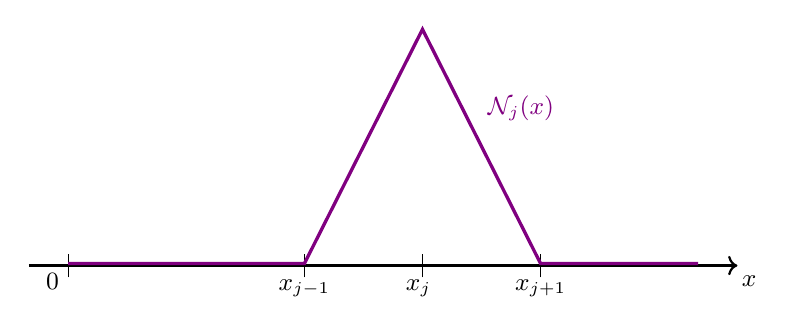
\begin{tikzpicture}
%\draw[fill=gray!23,gray!23](0,0) rectangle (11,4);
%\draw[step=0.5cm,gray,very thin] (0,0) grid (11,4); %background grid
\draw[thick,->] (0.5,1) -- (9.5,1)  ; 
\draw[-] (1,0.85) -- (1,1.15)  ; 
\draw[-] (4,0.85) -- (4,1.15)  ; 
\draw[-] (5.5,0.85) -- (5.5,1.15)  ; 
\draw[-] (7,0.85) -- (7,1.15)  ; 
\draw[very thick, violet] (1,1.025)--(4,1.025) -- (5.5,4) -- (7,1.025) --(9,1.025) ; 
\node[] at (6.75,3) {\small \color{violet} $\bN_j(x)$};
\node[] at (0.8,0.8) {\small $0$};
\node[] at (9.65,0.8) {\small $x$};
\node[] at (4,0.71) {\small $x_{j-1}$};
\node[] at (5.45,0.71) {\small $x_{j}$};
\node[] at (7,0.71) {\small $x_{j+1}$};
\end{tikzpicture}
\end{center}

Basis functions for $j=1$ and $j=nnx$ only contain the relevant half of the hat functions defined above.
Let us recall that an important property of these basis functions is that $\bN_i(x)$ is precisely one 
at node $x_i$ and zero on every other node.

%--------------------------------------------------------------------------
\subsection{Finite element solution}

Using the just defined basis functions we can define a finite element solution and finite element test functions as follows
\[
U(x,t) := \sum_{i=1}^{nnx} \bN_i(x)  U_i(t)
\]
\[
V(x) := \sum_{i=1}^{nnx} \bN_i(x)  V_i
\]

\paragraph{Definition 1.4.1} (Finite element formulation). 
Find $U(x,t)$ such that for all $t\in \R$ it holds that $U(\cdot,t)\in S^1$
and for all $V \in S^1$:
\[
a(U(x,t),V(x))=0
\]
and the following initial boundary conditions hold
\begin{align}
U(x=0,t) & = 0 & \forall t\in \R^+  \nn\\
U(x=L_x,t) & = 0 & \forall t\in \R^+ \nn\\
U(x,0) &= U_0(x) & \forall x\in[0,L_x] \nn\\
U_t(x,0) &= U_1(x) & \forall x\in[0,L_x] \label{eq:fdm-wave-4}
\end{align}
Note that because of the form $U$ takes, it does not have to hold that $U_0(x)$ equals $u_0(x)$.

For the finite element solution it is enough to test it only against the basis functions. This follows from the linearity of $a(u,v)$ in the second variable and therefore it holds that
\[
a(U(x,t),V(x))
=a\left(U(x,t), \sum_{i=1}^{nnx} \bN_j(x) V_j \right) 
=\sum_{i=j}^{nnx} V_j \; a\left(U(x,t),  \bN_j(x) \right) 
\]
Thus, if it holds for all of the basis functions $\bN_j$ , it also holds for all functions 
$V \in S^1$.

For each basis function $\bN_j(x)$ that is not on the edge, i.e. $j=2,...,nnx-1$ we can write using the definition of the bilinear form $a(\cdot,\cdot)$ (see Eq.~\eqref{eq:fdm-wave-aaa}):
\begin{eqnarray}
0 
&=& a\left(U(x,t),  \bN_j(x) \right)  \nn\\
&=&\int_0^L  \bN_j(x)  \frac{\partial^2 U}{\partial t^2}(x,t)  dx
+c^2 \int_0^L  \frac{\partial \bN_j}{\partial x}(x)  \frac{\partial U}{\partial x}(x,t)  dx \nn\\
&=&\int_0^L  \bN_j(x)  \frac{\partial^2 \left(\sum\limits_{i=1}^{nnx} \bN_i(x)  U_i(t) \right)}{\partial t^2}(x,t)  dx
+c^2 \int_0^L  \frac{\partial \bN_j}{\partial x}(x)  \frac{\partial \left(\sum\limits_{i=1}^{nnx} \bN_i(x)  U_i(t) \right)}{\partial x}(x,t)  dx \nn\\
&=&\sum\limits_{i=1}^{nnx} \frac{d^2  U_i(t) }{d t^2}  \int_0^L  \bN_j(x) \bN_i(x)   dx
+c^2 \sum\limits_{i=1}^{nnx} U_i(t)  \int_0^L  \frac{d \bN_j}{d x} (x) \frac{d \bN_i  }{d x}(x)  dx \nn\\
&=&\sum\limits_{i=1}^{nnx}   \ddot{U}_i(t)   \underbrace{\int_0^L  \bN_j(x) \bN_i(x)   dx}_{M_{ij}}
+c^2 \sum\limits_{i=1}^{nnx} U_i(t)  
\underbrace{\int_0^L  \frac{d \bN_j}{d x} (x) \frac{d \bN_i  }{d x}(x)  dx}_{K_{ij}} \nn\\
\end{eqnarray}
This results in $nnx-2$ linear ordinary differential equations.
For the two basis functions left out we can use
the boundary conditions imposed on $U$.
By defining the vector $\vec{\cal U}=(U_1(t),U_2(t),...U_{nnx}(t))$ 
we can use these $nnx$ linear differential equations to 
write the following ordinary differential equation
\begin{mdframed}[backgroundcolor=blue!5]
\begin{equation}
\M \cdot \vec{\ddot{{\cal U}}}(t) + c^2 \K \cdot \vec{\cal U}(t) = \vec{0}
\label{ss:waveq1}
\end{equation}
\end{mdframed}

The values of $M_{ij}$ and $K_{ij}$ can easily be calculated by splitting their integrals over all the elements like
\[
\int_0^{L_x} f(x) dx = \sum_{e=1}^{nelx} \int_{x_e}^{x_{e+1}} f(x) dx
\]
As the basis functions only have a maximum of two elements on which they are non-zero, the values of
Ti,j and Si,j can be calculated by just integrating over the few elements on which both basis functions are
non-zero. This allows us to calculate the following coefficients
\begin{eqnarray}
M_{i,i}&=&\int_0^L \bN_i(x) \bN_i(x) dx =\int_{x_{i-1}}^{x_{i+1}} \bN_i(x) \bN_i(x) dx = \frac23 h \nn\\
M_{i,i-1}&=&\int_0^L \bN_i(x) \bN_{i-1}(x)dx=\int_{x_{i-1}}^{x_{i}}\bN_i(x) \bN_{i-1}(x) dx=\frac16 h \nn\\
K_{i,i}&=&\int_0^L \bN_i'(x)\bN_i'(x) dx =\int_{x_{i-1}}^{x_{i+1}} \bN_i'(x) \bN_i'(x) dx = \frac{2}{h}\nn\\
K_{i,i-1}&=&\int_0^L \bN_i'(x)\bN_{i-1}'(x) dx =\int_{x_{i-1}}^{x_{i}} \bN_i'(x) \bN_{i-1}'(x) dx =-\frac{1}{h}
\end{eqnarray}
These integrals can easily be computed by hand in the 1D case but we will see that in most 2D,3D cases
this is not the case and we must resort to numerical quadrature.

%-----------------------------------------------------------------
\subsection{Time discretisation}

We can use a second-order approximation for the second-order derivative:
\[
\vec{\ddot{{\cal U}}}(t) \simeq  \frac{ \vec{\cal U}(t+ \delta t) -2 \vec{\cal U}(t) + \vec{\cal U}(t-\delta t)}{\delta t^2}
\]
which we can substitute in Eq.~\eqref{ss:waveq1}:
\[
\M \cdot \frac{ \vec{\cal U}(t+\delta t) -2 \vec{\cal U}(t) + \vec{\cal U}(t-\delta t)}{\delta t^2} 
+c^2 \K \cdot \vec{\cal U}(t) = \vec{0}
\]
Note that in the equation above the vector $\vec{\cal U}$ multiplying $\K$ is evaluated at time $t$. We will come back 
to this very shortly.
\[
\M \cdot ( \vec{\cal U}(t+\delta t) -2 \vec{\cal U}(t) + \vec{\cal U}(t- \delta t)) 
=- c^2 \delta t^2 \K \cdot \vec{\cal U}(t) 
\]
leading to finally write ({\color{orange} method \# 1}):
\begin{mdframed}[backgroundcolor=blue!5]
\[
\M \cdot  \vec{\cal U}(t+\delta t)
=\underbrace{ [2  \M  - c^2 \delta t^2 \K  ]  \cdot \vec{\cal U}(t) - \M \cdot \vec{\cal U}(t-\delta t)}_{\vec{b}}
\]
\end{mdframed}
which is of the form 
\[
{\cal \bm A} \cdot \vec{\cal U} (t+\delta t) = \vec{b}
\]
Alternatively we would have used an implicit approach by writing
\[
\M \cdot \frac{ \vec{\cal U}(t+\delta t) -2 \vec{\cal U}(t) + \vec{\cal U}(t-\delta t)}{\delta t^2} 
+c^2 \K \cdot \vec{\cal U}(t {\color{violet} +\delta t} ) = \vec{0},
\]
leading to write:
\begin{mdframed}[backgroundcolor=blue!5]
\[
(\M + c^2 \delta t^2 \K ) \cdot \vec{\cal U}(t+\delta t) = \underbrace{ \M \cdot(2 \vec{\cal U}(t) - \vec{\cal U}(t-\delta t)) }_{\vec{b}}
\] 
\end{mdframed}

\vspace{.5cm}

Given the presence of the terms $\vec{\cal U}(t)$ and $\vec{\cal U}(t-\delta t)$ in the equations above,
we can only solve the equation for $t \ge 2\delta t$ (assuming the time step $\delta t$ remains constant):
\[
\M \cdot  \vec{\cal U}(2\delta t)
= [2  \M  - c^2 \delta t^2 \K  ]  \cdot \vec{\cal U}(\delta t) - \M \cdot \vec{\cal U}(0)
\]
The value of $\vec{\cal U}(0)$ is known as it is the field at $t=0$ (initial condition). 
However, quid of $\vec{\cal U}(\delta t)$?
One way to avoid this problem is by using a 1st order Taylor expansion of this term:
\[
\vec{\cal U}(\delta t) = \vec{\cal U}(0) + \delta t \; \vec{\dot{{\cal U}}}(0)
\]
and since we know both terms in the rhs then all is well.

\vspace{.6cm}

Another approach can be taken ({\color{orange} method \# 2}): let us define 
\[
\vec{\cal V}=
\frac{ \vec{\cal U}(t+\delta t) -2 \vec{\cal U}(t) + \vec{\cal U}(t-\delta t)}{\delta t^2} 
\]
Then one needs to solve two equations one after the other:

\begin{mdframed}[backgroundcolor=blue!5]
\begin{eqnarray}
\M \cdot \vec{\cal V} &=&  -c^2 \K \cdot \vec{\cal U}(t) \nn\\
\vec{\cal U}(t+\delta t) &=& \delta t^2 \; \vec{\cal V} +2 \vec{\cal U}(t) - \vec{\cal U}(t-\delta t)
\end{eqnarray}
\end{mdframed}


\vspace{.6cm}

There is yet another option ({\color{orange} method \# 3}). 
Let us define this time $\vec{\cal W}(t)=\vec{\dot{{\cal U}}}(t)$.
Then Eq.~\eqref{ss:waveq1} can be written 
\[
\vec{\dot{{\cal W}}}(t) = \vec{\ddot{{\cal U}}} = -c^2 \M^{-1} 
\cdot \K \cdot \vec{\cal U}(t)
\]
Then we must solve the coupled set of equations:
\begin{align}
\vec{\dot{{\cal U}}}(t) &= \vec{\cal W}(t) \\
\vec{\dot{{\cal W}}}(t) &= -c^2 \M^{-1} \cdot \K \cdot \vec{\cal U}(t) 
\end{align}
with initial values
\begin{align}
\vec{\cal U}(0) &= \vec{\cal U}_0 \\ 
\vec{\cal W}(0) &= \vec{\dot{{\cal U}}}_0
\end{align}
We can also write (to first order)
\begin{align}
\frac{\vec{\cal U}(t+dt)-\vec{\cal U}(t) }{dt}    &= \vec{\cal W}(t) \\
\M \cdot \frac{\vec{\cal W}(t+dt)-\vec{\cal W}(t) }{dt}  &= -c^2 \; \K \cdot \vec{\cal U}(t) 
\end{align}
and finally
\begin{mdframed}[backgroundcolor=blue!5]
\begin{align}
\vec{\cal U}(t+dt) = \vec{\cal U}(t) + dt \; \vec{\dot{{\cal U}}}(t) \\
\M \cdot \frac{\vec{\dot{{\cal U}}}(t+dt)-\vec{\dot{{\cal U}}}(t) }{dt}  &= -c^2 \K \cdot \vec{\cal U}(t) 
\end{align}
\end{mdframed}
The first equation is straightforward and we then solve the second equation in a similar 
was as in method 2 to obtain $\vec{\dot{{\cal U}}}(t+dt)$.

Concretely, it goes as follows. Let us define 
$\vec{\cal R}= (\vec{\dot{{\cal U}}}(t+dt)-\vec{\dot{{\cal U}}}(t) )/dt$.
Then the second equation is $\M \cdot \vec{\cal R} = -c^2 \; \K \cdot \vec{\cal U}(t)$ 
and the algorithm goes 
as follows:
\begin{enumerate}
\item $\vec{\cal U}(t+dt) = \vec{\cal U}(t) + dt \; \vec{\dot{{\cal U}}}(t)$
\item solve $\M \cdot \vec{\cal R} = -c^2 \; \K \cdot \vec{\cal U}(t)$ 
\item recover $\vec{\dot{{\cal U}}}(t+dt) = \vec{\dot{{\cal U}}}(t) + dt \; \vec{\cal R}$
\end{enumerate}
This method is different than the other two because it keeps $\vec{\cal U}$ 
and its time-derivative as unknowns. 

Note that in all three cases the FE matrix is simply the mass matrix, 
which is good news since it tends to be nicely conditioned and symmetric.

This is all implemented in \stone~164. 

%-----------------------------------------------------
\subsection{The case of non-equidistant nodes and/or higher order elements}

In this section we will generalize the finite element method by first allowing irregular elements, i.e. 
elements of different size:
\begin{center}
\begin{tikzpicture}
%\draw[fill=gray!23,gray!23](0,0) rectangle (11,2);
%\draw[step=0.5cm,gray,very thin] (0,0) grid (11,2); %background grid
\draw[thick] (0.5,1) -- (2,1)  ; 
\draw[thick,dashed] (2,1) -- (4,1)  ; 
\draw[thick] (4,1) -- (8,1)  ; 
\draw[thick,dashed] (8,1) -- (9.5,1)  ; 
\draw[thick,->] (9.5,1) -- (11,1)  ; 
\draw[] (1,0.8)--(1,1.2);
\draw[] (4,0.8)--(4,1.2);
\draw[] (5.5,0.8)--(5.5,1.2);
\draw[] (7.5,0.8)--(7.5,1.2);
\draw[] (10,0.8)--(10,1.2);
\node[] at (0.9,0.6) {\small $a$};
\node[] at (4,0.6) {\small $x_{i-1}$};
\node[] at (5.45,0.6) {\small $x_{i}$};
\node[] at (7.5,0.6) {\small $x_{i+1}$};
\node[] at (9.9,0.6) {\small $b$};
\node[] at (11,0.76) {\small $x$};
\draw[<->] (4,1.5)--(5.45,1.5);
\draw[<->] (5.55,1.5)--(7.5,1.5);
\node[] at (4.75,1.7) {\small $h_{i-1}$};
\node[] at (6.5,1.7) {\small $h_i$};
\end{tikzpicture}
\end{center}

We divide an interval [a,b] with $a<b$ into $nelx$ elements separated by nodes. 
The nodes $x_i$ with $i=1,...nnx$ are chosen such that $a=x_1<x_2<...<x_{nnx-1} < x_{nnx}=b$
and the elements can then defined as
\[
e_i = [x_i,x_{i+1}] \qquad \text{for} \quad i=1,...,nnx
\]
with its size $h_i:=x_{i+1}-x_i$.

We have now two choices: either we define a so-called reference element (sometimes also called
canonical element) and establish the mapping from any real element to the reference one, later to be used in the 
formulation of the integrals, or we express the basis functions locally for each element and proceed by using these 
in the integrals.

For example the basis functions would then write 
\begin{align}
\bN_i(x) &= 0 & \text{if } &x < x_{i-1} \nn\\
\bN_i(x) &=  \frac{x-x_{i-1}}{x_i-x_{i-1}}& \text{if } & x\in [x_{i-1},x_{i}] \nn\\
\bN_i(x) &=  \frac{x_{i+1}-x}{x_{i+1}-x_i}   & \text{if } &x \in [x_{i},x_{i+1}] \nn\\
\bN_i(x) &= 0 & \text{if } &x >x_{i+1} \nn
\end{align}
as shown in the following figure:
\begin{center}
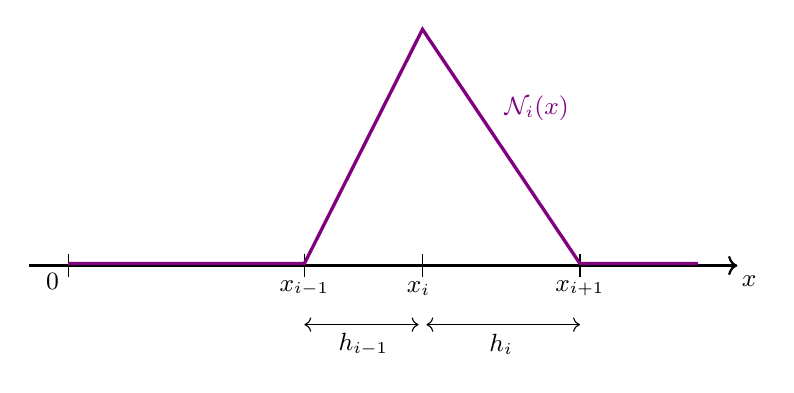
\begin{tikzpicture}
%\draw[fill=gray!23,gray!23](0,0) rectangle (11,4);
%\draw[step=0.5cm,gray,very thin] (0,0) grid (11,4); %background grid
\draw[thick,->] (0.5,1) -- (9.5,1)  ; 
\draw[-] (1,0.85) -- (1,1.15)  ; 
\draw[-] (4,0.85) -- (4,1.15)  ; 
\draw[-] (5.5,0.85) -- (5.5,1.15)  ; 
\draw[-] (7.5,0.85) -- (7.5,1.15)  ; 
\draw[very thick, violet] (1,1.025)--(4,1.025) -- (5.5,4) -- (7.5,1.025) --(9,1.025) ; 
\node[] at (6.95,3) {\small \color{violet} $\bN_i(x)$};
\node[] at (0.8,0.8) {\small $0$};
\node[] at (9.65,0.8) {\small $x$};
\node[] at (4,0.71) {\small $x_{i-1}$};
\node[] at (5.45,0.71) {\small $x_{i}$};
\node[] at (7.5,0.71) {\small $x_{i+1}$};

\draw[<->] (4,0.25)--(5.45,0.25);
\draw[<->] (5.55,0.25)--(7.5,0.25);
\node[] at (4.75,0) {\small $h_{i-1}$};
\node[] at (6.5,0) {\small $h_i$};
\end{tikzpicture}
\end{center}

Otherwise we would normally define the reference element $r=[-1,+1]$ and the 
basis functions inside the element attached to each node would be given by
\begin{eqnarray}
\bN_1(r) &=& \frac12 (1-r) \\
\bN_2(r) &=& \frac12 (1+r) 
\end{eqnarray}
We have of course already encountered these in Section~\ref{XYZ}.


The topic of higher-order elements has been covered in Section~\ref{} and poses no 
real difficulty. For example, 2nd-order elements would require an additional 
node in the middle of each element while the basis functions are defined on 
the reference element in section REF ... 

%-------------------------------------------------------------------------------------
\subsection{Conservation of energy}


The concept of conservation of energy is used all over physics and states most of the time that the total
amount of energy in a closed systems is constant. This conservation can also hold for the one-dimensional
wave equation and can be formulated as

\paragraph{Theorem} For a solution $u$ of the one-dimensional
wave equation there exists a constant $C>0$, independent of time $t$, such that
\begin{equation}
\left\|  \frac{\partial u}{\partial t} (\cdot, t)  \right\|^2 + 
c^2 \left\|  \frac{\partial u}{\partial x} (\cdot, t)  \right\|^2 =C \label{eq:fdm-wave-5}
\end{equation}
where $\| \cdot \|$ is the $L_2$-norm over the domain. 

\vspace{.5cm}

Proof: Let $v(x,t)=\frac{\partial u}{\partial t}(x,t)$ be the test function in the weak formulation of the one-dimensional wave equation. Using Eq.~\eqref{eq:fdm-wave-aaa}, this gives
\begin{eqnarray}
0 
&=& \int_D v(x,t) \frac{\partial^2 u}{\partial t^2}(x,t) dx + c^2 \int_D  \frac{\partial u}{\partial x}  \frac{\partial v}{\partial x} dx \nn\\
&=& \int_D \frac{\partial u}{\partial t}(x,t) \frac{\partial^2 u}{\partial t^2}(x,t) dx + c^2 \int_D  \frac{\partial u}{\partial x}  \frac{\partial }{\partial x} \frac{\partial u}{\partial t}(x,t) dx \nn\\
&=& \int_D \frac12 \frac{\partial}{\partial t} \left(\frac{\partial u}{\partial t} \right)^2 dx + c^2
\int_D  \frac12 \frac{\partial}{\partial t} \left( \frac{\partial u}{\partial x}  \right)^2  dx \nn\\
&=& \frac12 \frac{\partial}{\partial t} \int_D  \left(\frac{\partial u}{\partial t} \right)^2 dx + c^2
\frac12 \frac{\partial}{\partial t} \int_D   \left( \frac{\partial u}{\partial x}  \right)^2  dx \nn\\
&=& \frac12 \frac{\partial}{\partial t} 
\left(
\left\|  \frac{\partial u}{\partial t} (\cdot, t)  \right\|^2 + 
c^2 \left\|  \frac{\partial u}{\partial x} (\cdot, t)  \right\|^2
\right)
\end{eqnarray}
which implies Eq.~\eqref{eq:fdm-wave-5}.
This implies conservation of energy for the finite element solution of the wave equation.

From the above formulas we can define an energy function as $E(u,t)=\|\dot{u}\|^2  + c^2 \| \partial_x u \|^2 $, such that for a solution $u$ of the weak or finite element formulation there exists a constant $C>0$ 
such that $E(u,t)=C$ for all $t$.

Considering now the discrete solution $U$, the first error we can notice is that the initial values of the wave equation $u(x,0)$ and $\partial_t u(x,0)$ and its discretized value for the finite element formulation 
$U(x,0)$ and $\partial_t U(x,0)$ do not necessarily have the same energy,
or more specific, $E(u,0)$ and $E(U,0)$ do not have to be equal. But if we make the elements smaller and use
higher order polynomials for approximation, we can better approximate the original initial value with $U$ and
$\partial_t U$ and therefore better approximate the energy.

To analyse what happens to the energy when we discretize in time the system of ordinary differential equations
of Eq.~\eqref{ss:waveq1} we can use a more efficient way of calculating the energy. We can get this by putting the finite element $U(x,t)=\sum_{i=1}^{nnx} \bN_i(x) U_i(t)$ in the energy function, resulting in the following equations:

\begin{eqnarray}
E(U,t) 
&=& \left\|  \frac{\partial u}{\partial t} (\cdot, t)  \right\|^2 + 
c^2 \left\|  \frac{\partial u}{\partial x} (\cdot, t)  \right\|^2 \nn\\
&=& \int_D \left( \sum_{i=1}^{nnx} \bN_i(x) \dot{U}_i(t) \right)^2 dx 
+ c^2 \int_D \left( \sum_{i=1}^{nnx} \frac{d \bN_i}{dx}(x) U_i(t) \right)^2 dx \nn\\
&=& \int_D \sum_{i=1}^{nnx}\sum_{j=1}^{nnx} \bN_i(x) \bN_j(x) \dot{U}_i(t) \dot{U}_j(t) dx
+ c^2 \int_D \sum_{i=1}^{nnx}\sum_{j=1}^{nnx} \frac{d \bN_i}{dx}(x) \frac{d \bN_j}{dx}(x) U_i(t) U_j(t) dx\nn\\
&=& \sum_{i=1}^{nnx}\sum_{j=1}^{nnx} \dot{U}_i(t) \dot{U}_j(t)  \int_D  \bN_i(x) \bN_j(x) dx
+ c^2 \sum_{i=1}^{nnx}\sum_{j=1}^{nnx} U_i(t) U_j(t) \int_D  \frac{d \bN_i}{dx}(x) \frac{d \bN_j}{dx}(x)  dx\nn\\
&=& \sum_{i=1}^{nnx}\sum_{j=1}^{nnx} \dot{U}_i(t) \dot{U}_j(t) M_{ij} 
+ c^2 \sum_{i=1}^{nnx}\sum_{j=1}^{nnx} U_i(t) U_j(t) K_{ij} dx \nn\\
&=& \vec{\dot{{\cal U}}}^T \cdot \M \cdot \vec{\dot{{\cal U}}} 
+ c^2 \; \vec{\cal U}^T \cdot \K \cdot \vec{\cal U}
\end{eqnarray}
We see that methods 1\&2 might not be convenient when it comes to energy calculations since 
the time derivative of the $\vec{\cal U}$ vector does not appear explicitly, while it does
in method 3.

Because we know that real solutions of the wave equation and finite element formulation need to have a
constant energy, we can use the energy function as a measure of error over time when we have all the values
$U_i$ and $\dot{U}_i$ at a moment in time, like for the third method. We can even use this method this analyse
numerical solutions for which we don’t have the analytical solutions.

%---------------------------------------------------
\subsection{time step value \& CFL condition}






:




\newpage
%==============================================================================
\section{Solving the two-dimensional wave equation}




It simply writes
\[
\frac{\partial^2 u}{\partial t^2} = c^2 
\left( 
\frac{\partial^2 u}{\partial x^2} + 
\frac{\partial^2 u}{\partial y^2} 
\right)
\]
or also sometimes
\[
u_{tt} = c^2 (u_{xx} + u_{yy})
\]
Here to initial conditions and boundary conditions must be provided.


{\color{red} ... include here weak form derivation and discretisation ... }

We arrive again at the following equation
\begin{equation}
\M \cdot \vec{\ddot{{\cal U}}}(t) + c^2 \K \cdot \vec{\cal U}(t) = \vec{0}
\label{ss:waveq2d}
\end{equation}
At this stage a decision must be made, i.e. whether quadrilaterals or triangles 
are used, and whether they are linear, quadratic, etc ...



 %%%%%%%%%%%%%%%%%%%%%%%%%%%%%%%%%%%%%%%%%%%%%%%%%%%%%%%%%%%%%%%%%%%%%%%%%%%%

%%%%%%%%%%%%%%%%%%%%%%%%%%%%%%%%%%%%%%%%%%%%%%%%%%%%%%%%%%%%%%%%%%%%%%%%%%%%%%%%%%%%%%%%%%%%%%%%%%%
%\chapter{Computing derivatives of FEM primary variables} %%%%%%%%%%%%%%%%%%%%%%%%%%%%%%%%%%%%%%%%%
\chapter{Computing derivatives of FEM primary variables} \label{fem_derivatives} 
\begin{flushright} {\tiny {\color{gray} chapter\_fem\_derivatves.tex}} \end{flushright}
%~~~~~~~~~~~~~~~~~~~~~~~~~~~~~~~~~~~~~~~~~~~~~~~~~~~~~~~~~~~~~~~~~~~~~~~~~~~~~~~


 %%%%%%%%%%%%%%%%%%%%%%%%%%%%%%%%%%%%%%%%%%%%%%%%%%%%%%%%%%%%%%%%%

%%%%%%%%%%%%%%%%%%%%%%%%%%%%%%%%%%%%%%%%%%%%%%%%%%%%%%%%%%%%%%%%%%%%%%%%%%%%%%%%%%%%%%%%%%%%%%%%%%%
%\chapter{The Discontinuous Galerkin Finite Element Method (DG-FEM) \label{dgfem}} %%%%%%%%%%%%%%%%
\include{chapter_dg} %%%%%%%%%%%%%%%%%%%%%%%%%%%%%%%%%%%%%%%%%%%%%%%%%%%%%%%%%%%%%%%%%%%%%%%%%%%%%%

%%%%%%%%%%%%%%%%%%%%%%%%%%%%%%%%%%%%%%%%%%%%%%%%%%%%%%%%%%%%%%%%%%%%%%%%%%%%%%%%%%%%%%%%%%%%%%%%%%%
%\chapter{Tracking materials} %%%%%%%%%%%%%%%%%%%%%%%%%%%%%%%%%%%%%%%%%%%%%%%%%%%%%%%%%%%%%%%%%%%%%
\chapter{Tracking materials} %%%%%%%%%%%%%%%%%%%%%%%%%%%%%%%%%%%%%%%%%%%%%%%%%%%%%%%%%%%%%%%%%%%%%
\begin{flushright} {\tiny {\color{gray} \tt chapter\_tracking.tex}} \end{flushright}
%~~~~~~~~~~~~~~~~~~~~~~~~~~~~~~~~~~~~~~~~~~~~~~~~~~~~~~~~~~~~~~~~~~~~~~~~~~~~~~~~~~~~~~~~~~~~~~~~~~

%\section{Tracking materials and/or interfaces} 
\begin{flushright} {\tiny {\color{gray} tracking.tex}} \end{flushright}

Unless using a fully Lagrangian formulation, one needs an additional numerical method to represent/track
the various materials present in an undeformable (Eulerian) mesh.
The figure below (by B. Hillebrand) illustrates the three main methods used in geodynamics.

\begin{center}
\includegraphics[width=15cm]{images/tracking/tracking}
\end{center}

Note that what follows is applicable to FEM, FDM, etc ...


A typical test for advection algorithm is the Zalesak disk \cite{zale79}. It is a two dimensional test 
problem of solid body rotation with a constant angular velocity $\omega$ (in rad/sec):

\begin{center}
\includegraphics[width=6cm]{images/tracking/zale79a}
\includegraphics[width=6cm]{images/tracking/zale79b}\\
{\tiny Taken from \cite{zale79}. Left: Schematic representation of two dimensional 
solid body rotation problem. The field inside the cut out has value 3 and it is 1
outside. The rotational speed is such that one full revolution is effected in 
628 cycles. The width of the gap separating the two halves of the cylinder,
as well as the maximum extent of the "bridge" connecting the two halves, is 5 cells.
Right: Perspective view of initial conditions for the two dimensional! solid body rotation
problem. Note that only a $50\times50$ portion of the mesh centered on the cylinder is displayed.}
\end{center}

This benchmark is widely used in the literature \cite{stco91,supu00,vasv05,dilp06,basd08,zhbl14}.
Note that the Zalesak disc is often supplemented with a cone and a Gaussian features:

\begin{center}
\includegraphics[width=6cm]{images/tracking/leve96}\\
{\tiny Taken from \cite{leve96}. Initial data for solid rotation tests}
\end{center}

%..............................................
\subsubsection{The Particle-in-cell technique}\label{ss:pic}
\index{general}{Particle-in-Cell}  
\index{general}{Marker-and-Cell} 
\index{general}{PIC} 
\index{general}{MAC}

\begin{remark}
The terms 'particle' and 'marker' are commonly (and unfortunately) interchangeably used in the literature 
in the context of the particle-in-cell technique. However, one should be aware that the marker-and-cell (MAC) 
technique is something different: it was invented in the early 60's at the Los Alamos Laboratories by 
Harlow and Welch (1965) \cite{hawe65}. For more information on MAC see the review paper 
by McKee \etal (2008) \cite{mctf08}. 
Also, Tackley and King (2003) \cite{taki03} talk about the tracer-ratio method in the context of PIC... 
\end{remark}

The Particle-in-cell method is by far the most widely used in computational geodynamics. 
In its most basic form it is a rather simple method to implement and this probably owes to its success
and early adoption \cite{popo92}  in non-parallel codes such as \sopale \cite{full95}, 
I2VIS \cite{geyu03} or \citcoms \cite{mczh04} (Appendix~\ref{app:codes}).
It has been implemented in \aspect{} \cite{galh18} and the inherent load balancing issues arising from the 
parallel implementation as well as from the use of Adaptive Mesh Refinement are discussed. 
It has also been implemented in the MILAMIN code \cite{daks08} to study LLSVPs \cite{musd15}.

\begin{center}
\includegraphics[width=8cm]{images/tracking/crsg12}\\
{\captionfont One of the main problems of the PIC method is the fact that the interface 
between the fluid is not tracked explicitely, and if one uses a random distribution of 
particles the black dotted line reprensents the 'real' interface between the fluids 
while the red line is liekly to be the interface one would obtain based on the 
distribution of particles. Taken from Crameri \etal (2012) \cite{crsg12}.}
\end{center}

Samuel (2018) \cite{samu18} does a great job at explaining 
the core problem with PIC: {\it the method requires the method requires particle-mesh 
and mesh-particle mappings to be specified. These critical operations constitute a
major source of inaccuracy in the PIC solution \cite{mona85,dumg11,thmk14}. 
Indeed, while the Lagrangian advection alone is not prone
to significant numerical diffusion, particle–mesh mappings can introduce 
important amounts of dissipation. This is particularly true
when the spatial distribution of particles is not homogeneous, leading 
to areas in the vicinity of gridpoints that are not sufficiently
well sampled by particles, and other regions where the domain is
oversampled by particles. This recurrent sampling problem develops 
in regions characterized by strong deformation, and concerns
both compressible and incompressible flow \cite{waav15,pukp16}. 
The non-homogeneous sampling has two main
origins. \\
- The first one corresponds to inaccuracies in advecting the
Lagrangian particles \cite{meje04}. This aspect has drawn
the attention of a few recent studies \cite{waav15,pukp16}, 
which have proposed the use of conservative schemes to
map velocity components from the Eulerian grid to the Lagrangian
particles during their advection. Such schemes have shown to significantly 
improve the accuracy of the interpolation, and result in
a considerably more homogeneous spatial sampling. \\
- The second origin, which has received less attention, is related to the deforming
nature of the flow \cite{modm03}, and is completely independent 
of the accuracy of the numerical methods for interpolating
the velocities at particles’ locations. In fact, for a given velocity
field, particles should travel along their characteristics, and even in
the case of incompressible flows, the distance between characteristics 
can vary in general, and can strongly diverge or converge in
regions characterized by strong deformation. This naturally leads to
the development of a non-homogeneous spatial distribution of the
Lagrangian particles, even if the particles locations are perfectly
known.}



The basic methodology goes as follows:
\begin{enumerate}
\item distribute particles in the domain
\item assign a material identity (and/or any other quantity) to each of them
\item project particle quantities of the Eulerian nodes of the mesh
\item solve the Stokes equations for a new velocity field
\item interpolate the velocity onto the particles
\item move the particles with their respective velocities 
\item go back to step 3
\end{enumerate}  

As it turns out each step above needs to be carefully executed and is more difficult than it 
first looks. 

\paragraph{Distributing particles in the domain}. Let us assume we wish to distribute $N_p$ particles
in the domain. How large must $N_p$ be? To simplify, one end member could be 'as many particles as possible that fit in memory' 
while the other end member could be 'one per element/cell on average'. While the former does not necessarily guarantee a 
desired accuracy while being CPU and memory intensive, the latter will certainly lead to zones in the domain void 
of particles which will be problematic since the projection onto the mesh might yield zero values or very inaccurate values.
How many particles (per element/cell) will be enough?
Also, should the particles be randomly distributed in the domain or on some kind of regular grid? 
See \stone 13.

Taken from Tackley and King (2003) \cite{taki03}: "Tracers are initialized on a regular grid 
with each tracer perturbed from its grid position by a random amount of up to
$\pm$ half a grid spacing, in order to eliminate artifacts due to tracer alignment."


\paragraph{Averaging and projection}. This is a very critical step. Unfortunately, there is no community-wide
agreed-upon method. The problem at hand boils down to: at a given location $(\vec r)$ in space I need a
the value of a field which is carried by the particles. 
The first step is to find the particle(s) close to this point. If done naively, this is a very costly affair, 
and begs the question what 'close' means. Finding all particles within a radius $R$ of point $\vec r$ can 
be done very efficiently (e.g. with linked lists, Verlet lists, ...) but the choice 
of $R$ proves to be critical:
if too small, there may not be any particle inside the circle, and if too large there may be many particles 
inside the circle and the averaging over so many particles in space will prove to be over diffusive. 
In practice, the FD or FE mesh is used to provide an indication of $R$. 
In FDM, the four cells (or quarter cells) around
a node represent the volume of space containing the particles whose properties are to be averaged \cite{dumg11} 
as illustrated in the following figure:

\begin{center}
\includegraphics[width=12cm]{images/dumg11}\\
{\captionfont Taken from \cite{dumg11}. The "4-cell" and "1-cell" schemes for projecting 
properties defined on the markers (denoted by stars) onto a node (denoted by the solid circle). 
(A) The 4-cell scheme. The support of the interpolating function $N_i$ associated
with node $i$ is indicated by the shaded region. Only markers within the support of node $i$ 
contribute to the projection operation used to define the nodal value at $i$. The shape of 
the bilinear interpolation function for node $i$ is indicated in the lower frame. 
(B) The 1-cell scheme. The thick lines in the lower frame indicate the grid used to discretize the
Stokes equations, while the thin lines indicate the grid onto which marker properties are projected. 
The 1-cell scheme utilizes a compact support of size $\Delta x \times  \Delta y$. The support 
for nodes $r$, $s$, $t$ are indicated by the shaded regions. Only markers within the nodal 
support contribute to the projection operation for that node.}
\end{center}

Given that the FEM requires to compute integrals over each element, one could assume that 
only the particles inside the element will contribute 
to the average values assigned to the quadrature points (which I coin 'elemental approach'). 

However, one could also decide to first average the properties onto the nodes
before using these nodal values to assign values to the quadrature points (which I coin 'nodal approach'). 
In this case the FDM approach seen above could apply. 

Finally, in both FDM and FEM bi/trilinear basis functions are used for the interpolation as 
they can be interpreted as weighing functions. Higher order basis functions could also be used 
but the standard $Q_2$ basis functions (Section~\ref{sec:shpfct2d})
are 2-nd order polynomials which can take negative values (as opposed to the $Q_1$ 
basis functions which are strictly positive)
and this can pose problems: in some cases, although all values to be averaged are positive, 
their weighed average can be negative.
See Section~\ref{ss:bern} for concrete examples.

\underline{nodal approach}

\underline{elemental approach (1) - piece-wise constant interpolation} 

What follows is written with simplicity in mind, although more mathematical formulations 
can be found in the literature \cite{galh18}.

Assuming that we have established a list of particles tracking a field $f(\vec r)$ inside the 
element 
%and that each particle has an 
%associated weight $w_i$ (function of the location where the average is to be computed or not), 
we must now compute their average value $<f>$. 
The simplest approach which comes to mind is the arithmetic mean ($am$):
\[
\langle f\rangle_{am} = \frac{\sum\limits_{i=1}^n f_i}{n}
\]  
where $n$ is the number of particles inside the element.
In the case where $f$ is the (mass) density $\rho$, it is indeed what should be used. 
However, turning now to viscosity $\eta$, we know that its value can vary by many orders of magnitude 
over very short distances.
It is then likely that the average runs over values spanning values between 
$10^{18}\text{Pa s}$ and $10^{25} \text{Pa s}$.
As explained in \cite{scbe08} the arithmetic averaging tends to 'favour' large values: 
if the sum runs over 
10 particles, 9 carrying the value $10^{25}$ and 1 carrying the value $10^{19}$, 
the average value is then
\[
\langle\eta\rangle = \frac{9\cdot 10^{25}+1\cdot 10^{19}}{10} \simeq 0.9\cdot 10^{25}
\]
which is much much closer to $10^{25}$ than to $10^{19}$.
Other averagings are then commonly used, namely the geometric mean ($gm$)  and the 
harmonic mean ($hm$), defined as follows:
\[
\langle f\rangle_{gm} = \left( \prod_i f_i \right)^{1/n} 
\qquad
\text{or, }
\qquad
\log_{10} \langle f \rangle_{gm} = \frac{\sum\limits_{i=1}^{n} \log_{10} f_i }{n}  
\]
and 
\[
\langle f\rangle_{hm} = \left( \frac{\sum\limits_{i=1}^n \frac{1}{f_i} }{n}  \right)^{-1}
\qquad
\text{or, }
\qquad
\frac{1}{\langle f\rangle_{hm} } = \frac{\sum\limits_{i=1}^n  \frac{1}{f_i} }{n}  
\]
The geometric mean can be seen as a form of arithmetic mean of $\log_{10}$ values, 
while the harmonic mean can be seen as 
a form of arithmetic mean of the inverse values.

Looking back at the above example, the geometric mean of the viscosities is given by 
\[
\log \langle \eta\rangle_{gm} = \frac{9\cdot 25+1\cdot 19}{10} = 24.4 
\qquad \text{or,} \qquad 
\langle \eta\rangle_{gm} \simeq 2.5 \cdot 10^{24}
\]
and the harmonic mean:
\[
\langle\eta\rangle_{hm} \simeq \left( \frac{1}{10 \cdot  10^{19}} \right)^{-1} = 10^{20}
\]
We see that the harmonic mean tends to favour the small values. Also we recover the known property:
\begin{equation}
\langle f \rangle_{am}\quad  \geq \quad
\langle f \rangle_{gm}\quad  \geq \quad
\langle f \rangle_{hm} 
\end{equation}

%When all $f_i$ are equal to $f_0$ their computed average should also be equal to $f_0$. As a consequence the 
%weights $N_i$ should fulfil the condition $\sum\limits_{i=1}^n N_i=1$.
%If all weights are equal, then $N_i=1/n$ and the averagings become:

%\begin{equation}
%\langle f\rangle_{am} = \frac{1}{n} \sum\limits_{i=1}^n f_i
%\qquad
%\langle f\rangle_{gm} = \prod_i f_i^{1/n} 
%\qquad
%\langle f\rangle_{hm} = \left( \frac{1}{n}\sum_i^n \frac{1}{\phi_i} \right)^{-1}
%\end{equation}

Once a single average value has been computed for the whole element, then 
all quadrature points are assigned this value. 


\underline{elemental approach (2) - Least Squares Interpolation } 
One can revisit this topic on the grounds that 
with high(er) order elements optimal convergence is unlikely to be reached 
if viscosity (and density) are assumed to be constant inside each element (see  
\cite{galb19}). One could therefore use the least-square method to arrive at 
a functional representation of the field inside the element which is as 
close as possible (in the least-squares sense, then) to the particle-based field. 

Thielmann \etal (2014) \cite{thmk14} use the $Q_2P_{-1}$ element and introduce an element-wise interpolation
scheme based on a least squares fitting of the particle properties and choose the functional to 
be a linear function to match the pressure space. 
They define the error $\epsilon$ such that 
\[
\epsilon^2 = \sum_{i=1}^n ( \tilde{f}(x_i,y_i)-f_i)^2
\]
with $\tilde{f}(x,y)=a+bx+cy$. 
We then look for the minimum of $\epsilon^2$, i.e. $\vec\nabla(\epsilon^2)=0$ in the $\{a,b,c\}$ space.
So 
\begin{eqnarray}
0=\frac{\partial \epsilon^2}{\partial a} 
&=& 2\sum\limits_i ( \tilde{f}(x_i,y_i)-f_i) \nn\\
&=& 2\sum\limits_i ( a + bx_i +cy_i -f_i) \nn\\
&=& 2 \left[ a \sum\limits_i 1 + b \sum\limits_i x_i + c \sum y_i - \sum\limits_i f_i \right] \nn\\
0=\frac{\partial \epsilon^2}{\partial b} &=& 2\sum\limits_i ( \tilde{f}(x_i,y_i)-f_i) x_i \nn\\
&=& 2\sum\limits_i ( a + bx_i +cy_i -f_i) x_i \nn\\
&=& 2 \left[ a \sum\limits_i x_i  + b \sum\limits_i x_i^2 + c \sum x_i y_i - \sum\limits_i x_i f_i \right]\nn\\
0=\frac{\partial \epsilon^2}{\partial c} &=& 2\sum\limits_i ( \tilde{f}(x_i,y_i)-f_i) y_i \nn\\ 
&=& 2\sum\limits_i ( a + bx_i +cy_i -f_i) y_i \nn\\
&=& 2 \left[ a \sum\limits_i y_i + b \sum\limits_i x_i y_i + c \sum y_i^2 - \sum\limits_i y_if_i \right] \nn
\end{eqnarray}
so 
\[
\left( 
\begin{array}{ccc}
\sum\limits_i 1 & \sum\limits_i x_i & \sum\limits_i y_i \\
\sum\limits_i x_i & \sum\limits_i x_i^2 & \sum\limits_i x_iy_i \\
\sum\limits_i y_i & \sum\limits_i x_i y_i & \sum\limits_i y_i^2 
\end{array}
\right)
\cdot
\left(
\begin{array}{c}
a\\
b\\
c
\end{array}
\right)
=
\left(
\begin{array}{c}
\sum\limits_i f_i \\
\sum\limits_i x_i f_i \\
\sum\limits_i y_i f_i 
\end{array}
\right)
\]

We could also then decide to use a bi-linear function $\tilde{f}$, i.e.
\[
\tilde{f}(x,y)=a+bx+cy+dxy
\]
which lies in the $Q_1$ space of Taylor-Hood quadrilateral elements. In this case the error is 
\[
\epsilon^2 
= \sum_{i=1}^n ( \tilde{f}(x_i,y_i)-f_i)^2
= \sum_{i=1}^n (a+bx_i+cy_i + dx_iy_i -f_i)^2
\]
and one has to solve a $4\times 4$ system this time:
\[
\left( 
\begin{array}{cccc}
\sum\limits_i 1 & \sum\limits_i x_i & \sum\limits_i y_i & \sum\limits_i x_iy_i\\
\sum\limits_i x_i & \sum\limits_i x_i^2 & \sum\limits_i x_iy_i & \sum\limits_i x_i^2 y_i\\
\sum\limits_i y_i & \sum\limits_i x_i y_i & \sum\limits_i y_i^2 & \sum\limits_i x_iy_i^2\\ 
\sum\limits_i x_iy_i & \sum\limits_i x_i y_i & \sum\limits_i y_i^2 & \sum\limits_i x_i^2y_i^2  
\end{array}
\right)
\cdot
\left(
\begin{array}{c}
a\\
b\\
c\\
d
\end{array}
\right)
=
\left(
\begin{array}{c}
\sum\limits_i f_i \\
\sum\limits_i x_i f_i \\
\sum\limits_i y_i f_i \\
\sum\limits_i x_i y_i f_i 
\end{array}
\right)
\]


Once this linear system (or the previous one) has been solved we have obtained the coefficients $a,b,c(,d)$ 
which allow us to compute $\tilde{f}$ anywhere inside the element, and especially 
at the quadrature points. 

\begin{remark}
Using a different (bi)linear function $\tilde{f}$ for each element 
means that it is likely to be discontinuous 
from one element to another in regions of high gradients. 
\end{remark}

There is however one drawback with this approach (linear or bi-linear alike):
in the areas of steep gradients the computed coefficients can be such that 
the function $\tilde{f}$ evaluated on a quadrature point 
is negative  which 1) would be wrong but not numerically 
dramatic for density, 2) would be wrong and physically and numerically 
problematic for viscosity (a viscosity cannot be negative, and this would 
automatically destroy the SPD nature of the viscous block of the Stokes matrix).

This problem is discussed in Thielmann \etal (2014) in Section 3.2.1 and they 
call this "Over- and Under-shooting". A simple (iteratuve) 
fix is then designed which insures that the computed value is within user-defined 
acceptable bounds. This is also mentioned in \cite{galb19} but the authors 
explain that this problem was not encountered in the context of the publication.





\begin{remark}
Two variants of the PIC methods have been proposed: the Deformable PIC (DPIC) 
by Samuel (2018) \cite{samu18}, and the multiscale PIC in \cite{asmo12}.
\end{remark}

\begin{remark}
TO BE WRITTEN.
A word about the tracer ratio method. \cite{taki03}. 
Trim \etal (2020) show a modified method 
with a tracer repositioning algorithm designed to promote even tracer
coverage \cite{trlb20}. 
\end{remark}



See Stone~67 for a concrete example of Particle-In-Cell use and a detailed 
explanation of its implementation.



%.....................................................................
\paragraph{Interpolation of the velocity onto particles}.

Once the particle $i$ has been localised inside a given element (Section~\ref{sec:amiin}) 
and its reduced coordinates $(r,s,t)$ determined, the velocity at this location can 
be computed through the basis functions:
\[
\vec\upnu_i=\sum_{k=1}^m N_i(r,s,t) \vec\upnu_k
\]
This approach is not without problem: while the nodal velocities $\vec\upnu_k$ are such 
that\footnote{for incompressible flows, of course} 
$\vec\nabla\cdot\vec\upnu=0$ (in the weak sense), the computed velocity $\vec\upnu_i$ 
is not necessarily divergence-free! In order to remedy this, a 
Conservative Velocity Interpolation (CVI) has been proposed in \cite{waav15}.
Because the complete derivations for the CVI algorithm is quite large I 
have decided to make a new section about it (Section~\ref{sec:cvi}) rather than include it 
here.

%.....................................................................
\paragraph{Moving the particles}

This is discussed in the context of the Runge-Kutta Methods, see Section~\ref{sec:rkparticles}.



%..............................................
\subsubsection{The level set function technique}
\index{general}{Level-set Method} 
\index{general}{Level-set Function} 
\index{general}{LSM} 
\index{general}{LSF} 
\index{general}{ENO}

This method was developed in the 80's by Stanley Osher and James Sethian \cite{lofo06}

The Level-set Method (LSM), as it is commonly used in Computational Fluid Dynamics -- and especially 
in Computational Geodynamics -- represents a close curve $\Gamma$ (say, in our case, the 
interface between two fluids or layers) by means of a function $\phi$ (called the level-set function, or LSF).
$\Gamma$ is then the zero level-set of $\phi$:
\begin{equation}
\Gamma = \left\{ (x,y) \; |\; \phi(x,y)=0 \right\}
\end{equation}
The convention is that $\phi>0$ inside the region delimited by $\Gamma$ and $\phi<0$ outside.
The function value indicates on which side of the
interface a point is located (negative or positive) and this is
used to identify materials. 

Furthermore, if the curve $\Gamma$ moves with a velocity $\vec \upnu$, 
then it satisfies the following equation:
\begin{equation}
\frac{\partial \phi}{\partial t} + \vec\upnu \cdot \vec\nabla \phi = 0 
\end{equation}

The level set function is generally chosen to
be a signed distance function, i.e. $|\vec\nabla \phi| = 1$ everywhere 
and its value is also the distance to the interface.

As explained in \cite{hitg14}, the level-set function $\phi$ is advected 
with the velocity $\vec\upnu$ which is obtained by solving the Stokes equations.
This velocity does not guarantee that after an advection step the signed 
distance quality of the LSF is preserved. 
The LSF then needs to be corrected, which is also called reinitialisation. 
Finally, solving the advection equation must be done in an accurate manner both in time and space,
so that so-called ENO (essentially non-oscillatory) schemes are often employed for the 
space derivative \cite{ossh91,saev10}.


The level set method has not often been used in the geodynamics 
community with some notable exceptions 
\cite{bomh06,bomh07,habm07,grbh07,zlfd08,hagr10,sunh10,suhe10,hitg14}
An overview of the method and applications can
be found in \cite{osfe01}.

Several improvements upon the original LSM have been proposed, 
such as for instance the conservative level set of \cite{zhbl14}.
The most notable difference between CLS method originally proposed by Olsson \etal \cite{olkr05,olkz07}
and standard LS method lies in the choice of LS function. Instead of the signed distance function, the
CLS methods employ the Heaviside function $H(\phi)$ 
\[
H(\phi)=
\left\{
\begin{array}{ll}
1 & \phi>0 \\
1/2 & \phi=0 \\
0 & \phi<0
\end{array}
\right.
\]
where $\phi$ is the signed distance function as in the LSM. 
In practice, a hyperbolic tangent function is used:
\[
H(\phi) = \frac{1}{2} (1+\tan (\phi/2\epsilon))
\]
where $\epsilon$ defines the spreading width of $H$. In the case where there are only 
two fluids (i.e. a single level set is sufficient), the material properties such as density and viscosity
are computed as follows:
\[
\rho=\rho_1+(\rho_2-\rho_1)H(\phi)
\]
\[
\eta=\eta_1+(\eta_2-\eta_1)H(\phi)
\]

\Literature: \cite{vasv05,vasv08,migi07,vasv05b}. 
\begin{itemize}
\item Review of level-set methods \cite{gifo18}
\item Interactive 3-D computation of fault surfaces using level sets \cite{kadt08}
\end{itemize}

%..............................................
\subsubsection{The field/composition technique \label{sec:compfield}}
\index{general}{Compositional Field}

This is the approach taken by the \aspect{} developers \cite{krhb12,hedg17}. 
Each material $i$ is represented by a compositional field $c_i$, 
which takes values between 0 and 1.
Each compositional field is then advected with the (prescribed or computed) Stokes velocity \cite{chri92}:
\begin{equation}
\frac{\partial c_i}{\partial t} + {\bm v}\cdot {\bm \nabla }c_i = 0
\end{equation}
The value at a point (Finite element node or quadrature point) is 1 if it is in the 
domain covered by the material $i$, and 0 otherwise.
In one dimension, each compositional field is a Heavyside function. 
This approach is somewhat similar to the LSM but the field is essentially 
discontinuous across the interface, which makes it very difficult to advect.  
On the plus side, compositional fields need not be reinitialised, as opposed to LSF's.

Accurate numerical advection is a notoriously difficult problem. Unless very specialised 
techniques are used it often yields undershoot ($c_i<0$) and overshoot ($c_i>0$), which 
ultimately yields mass conservation issues. Also, unless special care is taken, 
compositional fields tend to become more and more diffuse over time: the SUPG method (Section~\ref{sec:supg})
and the entropy viscosity method \cite{krhb12,ropu19} add small amounts of diffusion to dampen the under- and 
overshoots. This means that at a given point two or more compositions may have values, 
which require some form of averaging. If under- and overshoots are present, these averagings
can become very problematic and even yield meaningless quantities (e.g. negative viscosities).

One rather old and popular filtering approach is the so-called Lenardic and Kaula (1993) \cite{leka93}
filter:

\begin{center}
\includegraphics[width=6cm]{images/compositions/leka93_filter1}\\
\includegraphics[width=6cm]{images/compositions/leka93_filter2}\\
{\captionfont Taken from Lenardic and Kaula \cite{leka93}}
\end{center}

\begin{center}
\includegraphics[width=16cm]{images/compositions/leka93_filter3}\\
{\captionfont From FENICS book}
\end{center}


\begin{center}
\includegraphics[width=8cm]{images/compositions/plth13}\\
{\captionfont 
Filtering approach proposed by Lenardic and Kaula (1993). 
The composition field $C$ is assumed to vary between 0 and 1. Grid points with $C$-values 
lower than 0 and greater than 1 are set to 0 and 1, respectively (red). 
$C_{min}$ and $C_{max}$ are the minimum and maximum spurious values observed. 
Grid points whose $C$-value is lower than $|C_{min}|$ or greater than ($2-C_{max}$) 
are also set to 0 and 1, respectively (blue). 
The $C$-value of all grid points that do not exhibit spurious oscillations (green) is then corrected
according to the difference between the original average composition and that computed after the reset-
ting of the spurious values.
Taken from Plesa \etal (2013) \cite{plth13}.}
\end{center}











\Literature: \cite{vyrc13}

Entropy viscosity method \cite{gupa11}

\improvement[inline]{write about DG approach}






%..............................................
\subsubsection{The Volume-of-Fluid method} 
\index{general}{Volume-of-Fluid Method}
\index{general}{VOF}

%from Napoleon \etal
The Volume-Of-Fluid (VOF) method is a fixed-grid approach based on the one-fluid model and considers that the various immiscible fluids (or `phases') can be described as a single fluid whose local physical properties, namely density and viscosity, vary in space and time depending on the volume fraction $C_i$ of each phase $i$ 
\cite{hini81,youn82}. 

The volume fraction of each fluid intrinsically obeys $\sum \limits_{{i=1}}^n C_i = 1$ where $n$ is the number of phases. 
Typically, $C_i=1$ in grid cells filled only with fluid $i$, and $0<C_i<1$ in grid cells cross--cut by an interface. 
There are two main classes of VOF methods: methods that try to reconstruct exactly the interface between fluids (e.g. \cite{puth18}), which requires significant computational time, and methods that do not, such as in JADIM and OpenFOAM. 
With no interface reconstruction, the thickness of the interfacial region is defined by $0<C_i<1$, and typically occupies two to three grid cells. 

\cite{hini81}\cite{ropu19}

See review of the method in Robey's phd thesis \cite{robe19}.


%..............................................
\subsubsection{The method of characteristics}

\todo[inline]{ask Arie to write something}

\cite{devv00a}

%.............................................
\subsubsection{The Marker Chain method}
\index{general}{Marker Chain method} 

In two dimensions, the idea is quite simple: each interface is discretised by means of a number
of Lagrangian points (which may or may not vary in time). The points are numbered and 
connected (think of the connectivity array of a 1D FEM code). In the case of small deformations, 
and in the absence of in/out-flow boundaries, the method is reasonably trivial to implement, and 
each couple of point defines a segment (and therefore its normal vector too) which can then be used
to answer the question: "at this location, am I above or below this interface" or "am I this domain our
outside this domain" (in the case that the interface does not reach any of the boundaries).

This method becomes somewhat impractical when large deformation occurs or, for example, 
when a domain splits into two (e.g. slab break off). One interface must then become two, 
and it requires an algorithm capable of detecting the breakup of the surface and capable 
of rebuilding/patching the new ones so that they can still be used further. 
Note that in case of large deformation some markers may get further and further apart 
from each other which makes for a poor representation of the surface. New markers should then 
be added but the question of when and where must then be addressed.

Also, switching to three dimensions can prove to be very difficult or simply very 
costly: the generation of the inital marker position is trivial but their connectivity 
can be complicated to establish at startup: for instance, a Stokes sphere will require
a mesh made of triangles which maps exactly the surface of the sphere (see \cite{thie18,moma19} 
for methods on how to efficiently produce such meshes). In the case of more complex 3D geometries
this may prove nearly impossible to do. So will the problem of splitting a surface into two 
(or merging two domains). \todo{I still have pics from the old days using \douar- include} 

This method is usually coupled to Eulerian meshes (typically with FDM, but not only). 
It was used in \cite{woid78} in the context of salt domes analysis and later in \cite{chri82,chyu84}.
It is also used in \cite{vaks97} but little details are given about the algorithms used
to track and update the chain in the presence of such large deformation.
It is also used (athough coupled to level set functions) in the \douar code\cite{brtf08} 
(see Section~\ref{app:codes}). Having worked myself on this code and having had to produce 
complex initial triangulated surfaces for simulations (see for example \cite{lobh10}) it is 
easy to understand why later users of this code did implement the marker-in-cell technique.
More recently, it is used to track the free surface position in a FDM code \cite{dumy16,chmd19}.

Finally, Christensen \cite{chri92} makes the following interesting comment:  
"One might assume that different methods 
of representing the discontinuity, for example, by a tracer chain \cite{chyu84} or a cloud of 
tracers, would solve these problems. However, the difficulties 
arise not only from the way in which material boundaries are 
represented. Physically, the rate of shear strain parallel to a 
rheological boundary is discontinuous. Within the finite ele-
ment scheme such jump can only be realized at an element 
boundary. In an Eulerian scheme, where the discontinuity will 
crosscut the elements, the jump in strain rate must be approx- 
imated by a continuous variation, and effectively, the rheolog-
ical properties on both sides of the discontinuity will be 
averaged in some way within the element."

Literature: Lin \& van Keken (2006) \cite{liva05,liva06a,liva06b,kaus05,mulyukova}

%..............................................
\subsubsection{Hybrid methods}

In Braun \etal \cite{brtf08} a level set method is presented which is based on a 3-D set
of triangulated points, which makes it a hybrid between tracers and level set functions:
in the \douar code (Appendix~\ref{app:codes}) the interface is then explicitely tracked by means of the tracers while the LSF is computed 
on the FE nodes. Although very promising in theory, this method proved to be difficult to use in practice
since it requires a) a triangulation of the interfaces at $t=0$ which is not trivial if the geometries
are complex (think about a slab in 3D); b) the addition or removal of tracers because of the interface deformation
and the patching of the triangulation; c) the calculation of the distance to the interfaces for each 
FE node based on the triangle normal vectors. 
This probably explains why the Particle-In-Cell method was later implemented in this code (pers. comm.).
Note that another very similar approach is used in \cite{saev10}.



%..............................................
\subsubsection{Boundary fitted mesh}

This method is rather simple to implement and works well for small deformations. It is 
for instance used by Frehner \cite{freh14} (see online supplementary material) in which it is 
stated: "The numerical grid is set up in such a way that the interface
between different material phases (two layers in this case) coincides with element boundaries. Hence, each
element belongs to a unique material phase and no interpolation is necessary."
With such a method, each element is initally attributed a material phase/number and its material
properties do not change. 


\vspace{2cm} 

\Literature: three-dimensional front tracking method using a triangular mesh \cite{sclo03}.







 

\newpage 

%\section{Conservative Velocity Interpolation (CVI)} 
%\label{sec:cvi}\begin{flushright} {\tiny {\color{gray} \tt cvi.tex}} \end{flushright}
%~~~~~~~~~~~~~~~~~~~~~~~~~~~~~~~~~~~~~~~~~~~~~~~~~~~~~~~~~~~~~~~~~~~~~~~~~~~~~~~~~~~~~~~~~~~~~~~~~~


To my knowledge the conservative velocity interpolation (CVI) was introduced to 
the computational geodynamics community in \textcite{waav15} (2015). 
As mentioned in the paper  ``An improved velocity interpolation scheme that conserves the divergence 
of the flow field has been developed by \textcite{jepm01} (2001) and the simplified scheme for incompressible 
flow (i.e., divergence free) has been demonstrated that it largely eliminates the spurious 
distribution of particles for 2D incompressible flow problem (see \textcite{meje04} (2004)).''

Additional more recent publications on the topic of accurate marker 
advection: \textcite{simw21} (2021), \textcite{siwv22} (2022).

%-------------------------------------------------------------
\subsection{A few remarks about Wang \etal (2015)}

The article by \textcite{waav15} (2015) comes with supplementary material with more details 
on the derivation of the corrective velocities but that material is a Word
document printed to pdf with an annoying layout of equations, different font sizes,
lack of alignment, etc ... Also, Fig.~1 of the paper is reproduced here:
\begin{center}
\includegraphics[width=4cm]{images/cvi/wang15}
\end{center}
Why the authors chose to label nodes a,b,...h and not 1,2,...8 shall forever remain 
a mystery, but it is not as problematic as the labelling of the axes:
indeed, if $X_1$ is the $x$-axis then $X_3$ should be the $y$-axis 
and $X_2$ the $z$-axis. That is quite illogical. Or is it a mistake in 
the drawing only? In any case this sheds some confusion on the equations 
presented in the paper so I have decided to carry out all the CVI derivations 
in this chapter.

Their paper does not seem to consider cases where the element is not a 
cuboid (so what about CitcomS, or ALE formulations?), nor does it address higher order elements. 
Finally many details of the setups in the paper are just not there and I had to 
email the author(s) multiple time regarding:

\begin{itemize}
\item the setup of the couette flow in section 3.1 is 
incomplete: for instance, size of the box ? velocity value ? exact 
formula for the vel field (couette flow, I know, but how thick are the 
layers before rotation)? etc ...\\
Wang answered me: ``The box is a unit box (nondimentional 1*1). I attached the function for 
the analytical solution for the exact formula for the velocity field that you asked. I didn't 
find the models file yet, so I can't tell you what it is the value of the velocity. 
But I think it can be: 1m*1m box with 1m/s on the surface (V0).
In Citcom, the timestep is chosen to let any material in one cell not to move more than half
of the cell length (CFL=0.5). Then we have this parameter "finetunedt" ($<1$) to multiply it. I remember
I usually use 0.9 or 0.7.  So the CFL=0.45 or 0.35. 
Concerning the Couette flow we used a viscosity of 1e3, 
which make very sharp velocity contrast across the diagonal line.''
\begin{small}
\begin{verbatim}
for (i=1;i<=E->lmesh.nno;i++)
{     
x =  E->X[1][i]; 
z =  E->X[2][i];
eta1=E->control.testvelval[1];
eta2=E->control.testvelval[2];
alpha=E->control.testvelval[3]*PI/180;  /*coordinate rotation angle */
V0=E->control.testvelval[4];
h=sqrt(2.0)*sin(alpha+PI/4); /*WHL: h (with analytical solution) is a function of the rotation angle */
V1=(x*sin(alpha)+z*cos(alpha))*2*V0*eta2/(eta1+eta2)/h;
V2=(x*sin(alpha)+z*cos(alpha))*2*V0*eta1/(eta1+eta2)/h+(eta2-eta1)*V0/(eta1+eta2);
if (x*sin(alpha)+z*cos(alpha)<0.5*h)          
{
E->V[1][i]=V1*cos(alpha);
E->V[2][i]=-V1*sin(alpha);
}
else
{
E->V[1][i]=V2*cos(alpha);
E->V[2][i]=-V2*sin(alpha);
}
if (E->mesh.nsd == 3)
E->V[3][i]=0.;
}
\end{verbatim}
\end{small}

\item which advection scheme was used and 
I am worried that at no point in the publication the timestep size is 
either mentioned nor its importance discussed.\\
Wang answered: ``About the timestep, my experience is that using smaller timestep 
would't solve this kind of problem. Otherwise we probably
would not need to use this new velocity interpolation.  I could not remember that I tested 
the effects of timestep for this model. So it would be nice to know the result if you test it.  
The advection scheme is the 2nd Runge Kutta. ''

\item Agrusta wrote: "here the input values for the couette flow: 
testvelval=100000,1,45,0.01    \# eta1,eta2,angle,velocity. mesh = 33x33. 
initial tracers 100X100, random distribution"

\end{itemize}

Looking at their Fig.~2a,b we see black arrow tips in the blue region where 
velocity should be zero. Velocity is indeed zero and the authors confirmed that 
the arrow tips are an artefact of their visualisation software (!).

\Literature: 
McNally (2011) \cite{mcna11} proposed
a divergence-free interpolation of vector fields from point values in the context 
of magnetohydrodynamics. \textcite{pukp16} (2016) has applied the CVI to staggered grid FDM.

 
%-------------------------------------------------------------
\subsection{In 2D with $Q_1$ basis functions - Naive approach}

Let us start directly in reduced coordinates $(r,s)\in [-1:1]^2$ (i.e. the reference element).
The velocity components inside of the element are given by:
\begin{eqnarray}
u^h(r,s)&=&\sum_i \bN_i(r,s) u_i \nn\\
v^h(r,s)&=&\sum_i \bN_i(r,s) v_i \nn
\end{eqnarray}
where $\bN_i$ are the four $Q_1$ basis functions defined as follows:
\begin{eqnarray}
\bN_1(r,s)&=& \frac{1}{4}(1-r)(1-s)  \nonumber\\ 
\bN_2(r,s)&=& \frac{1}{4}(1+r)(1-s)  \nonumber\\ 
\bN_3(r,s)&=& \frac{1}{4}(1+r)(1+s)  \nonumber\\ 
\bN_4(r,s)&=& \frac{1}{4}(1-r)(1+s)  \nonumber
\end{eqnarray}
The incompressibility constraint in the $(r,s)-$coordinate system reads
\[
(\vec\nabla\cdot\vec\upnu)^h=
\frac{\partial u^h}{\partial r}+
\frac{\partial v^h}{\partial s}
=
\sum_i \left(  
\frac{\partial \bN_i}{\partial r} u_i+
\frac{\partial \bN_i}{\partial s} v_i
\right)
=0.
\]
However, it is trivial to verify that the incompressibility 
condition is not and \textit{can not} be verified for all values of  
$r,s \in [-1,1]^2$.
It would then make sense to think of a corrective term to the interpolation
which would add just enough degrees of freedoms so as to insure an exact\footnote{more
on this later} incompressibility in the element. 
Let us then write:
\begin{eqnarray}
u^h(r,s)&=&\sum_i \bN_i(r,s) u_i + (a s + b)(1-r)(1+r) \nn\\
v^h(r,s)&=&\sum_i \bN_i(r,s) v_i + (c r + d)(1-s)(1+s) \nn
\end{eqnarray}
Note that in this way the correction is zero on the $x=-1$ and $x=+1$ sides 
of the element for $u$, and likewise for $v$ on the top and bottom sides (in 
other words the velocity remains continuous from one element to another).
In this case,
\begin{eqnarray}
\frac{\partial u^h}{\partial r}&=&\sum_i \frac{\partial \bN_i}{\partial r} u_i + (a s + b) (-2r) \nn\\
\frac{\partial v^h}{\partial s}&=&\sum_i \frac{\partial \bN_i}{\partial s} v_i + (c r + d)(-2s) \nn
\end{eqnarray}
We have introduced 4 coefficients  $(a,b,c,d)$ which remain to be determined. 
We start with:
\begin{eqnarray}
\sum_i \frac{\partial N_i}{\partial r} u_i 
&=& -\frac{1}{4} (1-s) u_1 + \frac{1}{4} (1-s) u_2 +\frac{1}{4} (1+s) u_3 -\frac{1}{4} (1+s) u_4 \nn\\
&=& (1-s) \frac{u_2-u_1}{4} + (1+s) \frac{u_3-u_4}{4} \nn\\
&=& (1-s) u_{21} + (1+s) u_{34} \nn\\
\sum_i \frac{\partial N_i}{\partial s} v_i 
&=& -\frac{1}{4} (1-r) v_1 - \frac{1}{4} (1+r) v_2 +\frac{1}{4} (1+r) v_3 +\frac{1}{4} (1-r) v_4 \nn\\
&=& (1-r) \frac{v_4-v_1}{4} + (1+r)\frac{v_3-v_2}{4} \nn\\
&=& (1-r) v_{41} + (1+r) v_{32} \nn
\end{eqnarray}
where $u_{ij}=(u_i-u_j)/4$ and $v_{ij}=(v_i-v_j)/4$, so that in the end
\begin{eqnarray}
\frac{\partial u^h}{\partial r} &=& (1-s) u_{21} + (1+s) u_{34} + (a s + b)(-2r) \\
\frac{\partial v^h}{\partial s} &=& (1-r) v_{41} + (1+r) v_{32} + (c r + d)(-2s)
\end{eqnarray}
The incompressibility condition is now:
\[
(\vec\nabla\cdot\vec\upnu)^h =
(1-s) u_{21} + (1+s) u_{34} 
+ (a s + b) (-2r) +
(1-r) v_{41} + (1+r) v_{32}
+ (c r + d)(-2s)
=0
\]
This can be rewritten as
\[
(\vec\nabla\cdot\vec\upnu)^h =
C_0  + C_1 r + C_2 s + C_3 rs = 0
\]
where the four $C_i$ coefficients are functions of the velocities and the other coefficients.
In order for this expression to be exactly zero {\it everywhere}, each $C$ coefficient has
to be independently zero.

\begin{eqnarray}
C_0   &(.)  &  u_{21} + u_{34} + v_{41} + v_{32} =0\nn\\ 
C_1   &(r)  &  -v_{41} + v_{32} -2b =0\nn\\ 
C_2   &(s)  &  -u_{21} + u_{34} -2d =0 \nn\\ 
C_3   &(rs) &  -2a -2c =0\nn 
\end{eqnarray}

The first line is simply the incompressibility condition
expressed in the center of the element (i.e. $r=s=0$),
so we set it aside for now (I will come back to it later!)
and focus on the remaining three.

At this stage it is important to note that in the absence of corrective terms (i.e. $a=b=c=d=0$)
then only $C_3=0$ and the divergence inside the element is a linear field.

We obtain
\[
c=-a
\qquad
b=\frac{1}{2}(-v_{41} + v_{32})
\qquad
d=\frac{1}{2} (-u_{21} + u_{34})
\]
Since $a$ and $c$ are not otherwise constrained, we can set them to zero, and we then have:
\[
b=\frac{1}{2}(v_{14} + v_{32})
\quad\quad
d=\frac{1}{2} (u_{12} + u_{34})
\]
and finally
\begin{eqnarray}
u^h(r,s)
&=&\sum_i \bN_i(r,s) u_i + b(1-r)(1+r) 
=\sum_i \bN_i(r,s) u_i + \frac{1}{2}(v_{14} + v_{32})(1-r)(1+r) \nn\\
v^h(r,s)
&=&\sum_i \bN_i(r,s) v_i + d(1-s)(1+s) 
=\sum_i \bN_i(r,s) v_i + \frac{1}{2} (u_{12} + u_{34})(1-s)(1+s) \nn
\end{eqnarray}

By using these corrected interpolations for both components 
of the velocity then one ensures that a point-wise divergence free
velocity field anywhere in the element.
However, these derivations were carried out in the reference element. 
In fact they would work also for rectangular elements with minimal 
changes, but not for generic quadrilaterals.

To be clear, let us now compute the velocity divergence of the corrected 
velocity field above:
\begin{eqnarray}
(\vec\nabla\cdot\vec\upnu)^h 
&=&
\frac{\partial u^h}{\partial r}+
\frac{\partial v^h}{\partial s}
\nn\\
&=& (1-s) u_{21} + (1+s) u_{34} +  \frac{1}{2}(v_{14} + v_{32})(-2r)
+ (1-r) v_{41} + (1+r) v_{32}  + \frac{1}{2} (u_{12} + u_{34})(-2s) \nn\\
&=& u_{21} + u_{34} + v_{41} + v_{32}
-s u_{21} + s u_{34} -r v_{14} -r v_{32} 
-r v_{41} + r v_{32} -s u_{12} -s u_{34} \nn\\
&=& u_{21} + u_{34} + v_{41} + v_{32} 
\end{eqnarray}
A point must then be made crystal clear: the divergence is
{\it not} zero. The quantity above is constant inside the element 
(it does not depend on $r$ nor $s$). 
{\bf All what the CVI algorithm does is to remove the spatial dependence
of the velocity divergence inside the element}.

%-------------------------------------------------------------------
\subsection{In 2D with $Q_1$ basis functions - better approach}

We now consider a generic quadrilateral in the $x,y$-coordinate space and its equivalent in the 
reference space $r,s$. One can easily show that the gradient of a field $f$ verifies 
\[
\left(
\begin{array}{c}
\frac{\partial f}{\partial x} \\ \\
\frac{\partial f}{\partial y} 
\end{array}
\right)
=
\tilde{\bm J} \cdot
\left(
\begin{array}{c}
\frac{\partial f}{\partial r} \\ \\
\frac{\partial f}{\partial s} 
\end{array}
\right)
\]
where $\tilde{\bm J}$ in the inverse of the Jacobian matrix.
We then postulate again
\begin{eqnarray}
u^h(r,s)&=&\sum_i \bN_i(r,s) u_i + (a s + b)(1-r)(1+r) \nn\\
v^h(r,s)&=&\sum_i \bN_i(r,s) v_i + (c r + d)(1-s)(1+s) \nn
\end{eqnarray}
In this case,
\begin{eqnarray}
\frac{\partial u^h}{\partial r}&=&\sum_i \frac{\partial \bN_i}{\partial r} u_i + (a s + b) (-2r)   \nn\\
\frac{\partial u^h}{\partial s}&=&\sum_i \frac{\partial \bN_i}{\partial s} u_i + a (1-r^2) \nn\\
\frac{\partial v^h}{\partial r}&=&\sum_i \frac{\partial \bN_i}{\partial s} v_i + c (1-s^2) \nn\\
\frac{\partial v^h}{\partial s}&=&\sum_i \frac{\partial \bN_i}{\partial s} v_i + (c r + d)(-2s) \nn
\end{eqnarray}
We have introduced 4 coefficients  $(a,b,c,d)$ which remain to be determined.
In order to compute the velocity divergence inside the element we will need 
\begin{eqnarray}
\frac{\partial u}{\partial x} 
&=& \tilde{J}_{xx} \frac{\partial u}{\partial r} +  \tilde{J}_{xy} \frac{\partial u}{\partial s}  \nn\\
&=& \tilde{J}_{xx} \left( \sum_i \frac{\partial \bN_i}{\partial r} u_i + (a s + b) (-2r)  \right) 
 +  \tilde{J}_{xy} \left( \sum_i \frac{\partial \bN_i}{\partial s} u_i + a (1-r^2) \right)  \nn\\
&=& \tilde{J}_{xx} \left(  -(1-s) u_{12} + (1+s) u_{34} + (a s + b) (-2r)  \right) \nn\\ 
&+&  \tilde{J}_{xy} \left(  -(1-r) u_{14} - (1+r) u_{23} + a (1-r^2) \right)
\nn\\
\frac{\partial v}{\partial y} 
&=& \tilde{J}_{yx} \left(  -(1-s) v_{12} + (1+s) v_{34} + c (1-s^2)   \right)  \nn\\
&+&  \tilde{J}_{yy} \left(  -(1-r) v_{14} - (1+r) v_{23} + (cr+d) (-2s) \right) \nn
\end{eqnarray}
where $u_{ij}=(u_i-u_j)/4$ and $v_{ij}=(v_i-v_j)/4$.
The velocity divergence can be written as follows
\[
\frac{\partial u}{\partial x} 
+\frac{\partial v}{\partial y} = C_0 +C_1 r + C_2 s + C_3 rs + C_4 r^2 + C_5 s^2 =0
\]
with
\begin{eqnarray}
C_0 &=& J_{xx} (-u_{12} + u_{34} ) + J_{xy} (- u_{14} - u_{23} )  + J_{yx}  (-v_{12} + v_{34}) + J_{yy} (-v_{14} - v_{23} )  \nn\\ 
C_1 &=& J_{xy} (u_{14} - u_{23}) + J_{yy} (v_{14} - v_{23}) - 2 b J_{xx}   \nn\\ 
C_2 &=& J_{xx} (u_{12} + u_{34}) + J_{yx} ( v_{12} + v_{34} )  - 2 d J_{yy}    \nn\\ 
C_3 &=& -2 a J_{xx}  -2 c J_{yy} \nn\\ 
C_4 &=& -a J_{xy}  \nn\\
C_5 &=& -c J_{yx}  \nn\\
\end{eqnarray}
where the six $C_i$ coefficients are functions of the velocities and the other coefficients.
In order for this expression to be exactly null {\it everywhere}\footnote{We know by now 
that this is not possible}, each $C$ coefficient has
to be independently null.

This immediately yields $a=c=0$ (since the components of the $\tilde{\bm J}$ tensor
are not necessarily zero - and if $J_{xy}$ and $J_{yx}$ are zero then the equation 
for $C_3$ remains and we would still take $a=c=0$ for simplicity) 
and the equation for $C_3$ is immediately satisfied.
We then have:
\begin{eqnarray}
b&=&\frac{1}{2J_{xx}} ( J_{xy} (u_{14} - u_{23}) + J_{yy} (v_{14} - v_{23})  )  \nn\\
d&=&\frac{1}{2J_{yy}} ( J_{xx} (u_{12} + u_{34}) + J_{yx} ( v_{12} + v_{34} ) ) \nn
\end{eqnarray}
These expressions contain the same ingredients as before but also 
introduce more coupling between the velocity components. 
If the element is rectangular then $J_{xy}=J_{yx}=0$ and 
\begin{eqnarray}
b&=&\frac{J_{yy}}{2J_{xx}} ( v_{14} - v_{23} ) \nn\\
d&=&\frac{J_{xx}}{2J_{yy}} ( u_{12} + u_{34} ) \nn
\end{eqnarray}
If the element is square then $J_{xx}=J_{yy}=0$ so 
\begin{eqnarray}
b&=&\frac{1}{2} ( v_{14} - v_{23} ) \nn\\
d&=&\frac{1}{2} ( u_{12} + u_{34} ) \nn
\end{eqnarray}
and finally the velocity correction is 
\begin{eqnarray}
\delta u&=&\frac{1}{2} ( v_{14} - v_{23} ) (1-r)(1+r)\nn\\
\delta v&=&\frac{1}{2} ( u_{12} + u_{34} ) (1-s)(1+s)\label{eq:cvi_corr1}
\end{eqnarray}

%-------------------------------------------------------------------
\subsection{Comparison with Wang \etal (2015) for 2D}

Rather annoyingly Wang \etal (2015) use a reference element that is $[0,1]\times[0,1]$
as opposed to the standard $[-1,1]\times[-1,1]$:
\begin{center}
\fbox{\includegraphics[width=12cm]{images/cvi/wang15_b}}\\
{\captionfont Taken from the supplementary material of Wang \etal (2015).}
\end{center}
Since basis functions must be 1 on their node, then the numbering must be as follows:
\begin{verbatim}
c--d            4--3
|  |     <=>    |  |
a--b            1--2
\end{verbatim}
Setting $\Delta x_1=\Delta x_2=1$, replacing $a$ by $1$, $b$ by 2, 
$c$ by 4 and $d$ by 3, $x_1$ by $r'$ and $x_2$ by $s'$, $U_1$ by $u$
and $U_2$ by $v$, we arrive at 
(in order to render the notations a bit lighter I have set $U=U_1$ and $V=U_2$)
\begin{eqnarray}
\Delta U &=& \frac12 r'(1-r')(v_1-v_2-v_4+v_3) = \frac12 r'(1-r')(4v_{14}-4v_{23}) \nn\\
\Delta V &=& \frac12 s'(1-s')(u_1-u_2-u_4+u_3) = \frac12 s'(1-s')(4u_{12}+4u_{34}) \nn
\end{eqnarray}
Since $r=2r'-1$ and $s=2s'-1$ then we find that 
\begin{eqnarray}
\Delta U &=& \frac12 (1-r^2)(v_{14}-v_{23}) \nn\\
\Delta V &=& \frac12 (1-s^2)(u_{12}+u_{34})
\end{eqnarray}
which is Eq.~\eqref{eq:cvi_corr1}. In the case of the reference element then 
my velocity corrections are identical to theirs.

Let us look at the equations of the figure above. 
Since the authors state that they ``transform the rectangular cells into unit squares'' 
we do away with $\Delta x_1 = \Delta x_2 = 1$. Eqs. 3 and 1 together yield:
\begin{eqnarray}
U&=&(1-x_1)(1-x_2) U^a+x_1(1-x_2)U^b + (1-x_1)x_2 U^c + x_1x_2 U^d
+ \frac12 x_1(1-x_1)(V^a-V^b-V^c+V^d) \nn\\
V&=&(1-x_1)(1-x_2) V^a+x_1(1-x_2)V^b + (1-x_1)x_2 V^c + x_1x_2 V^d
+ \frac12 x_2(1-x_2)(U^a-U^b-U^c+U^d) \nn
\end{eqnarray}
Then 
\begin{eqnarray}
\frac{\partial U}{\partial x_1} 
&=& -(1-x_2) U^a+(1-x_2)U^b -x_2 U^c + x_2 U^d + \frac12 (1-2x_1)(V^a-V^b-V^c+V^d) \nn\\
\frac{\partial V}{\partial x_2}
&=& -(1-x_1) V^a - x_1V^b + (1-x_1) V^c + x_1 V^d + \frac12 (1-2x_2)(U^a-U^b-U^c+U^d) \nn
\end{eqnarray}
So 
\begin{eqnarray}
\frac{\partial U}{\partial x_1} \! + \! \frac{\partial V}{\partial x_2} 
&=&
-(1-x_2) U^a+(1-x_2)U^b -x_2 U^c + x_2 U^d + \frac12 (1-2x_1)(V^a-V^b-V^c+V^d) \nonumber\\
&&-(1-x_1) V^a - x_1V^b + (1-x_1) V^c + x_1 V^d + \frac12 (1-2x_2)(U^a-U^b-U^c+U^d) \nonumber\\
&=& -U^a + U^b + x_2(U^a-U^b-U^c+U^d) + \frac12 (V^a-V^b-V^c+V^d)
-x_1 (V^a-V^b-V^c+V^d) \nonumber\\
&& -V^a+V^c + x_1(V^a-V^b-V^c+V^d) + \frac12 (U^a-U^b-U^c+U^d)
-x_2 (U^a-U^b-U^c+U^d) \nonumber\\
&=& -U^a + U^b  + \frac12 (V^a-V^b-V^c+V^d)
 -V^a+V^c  + \frac12 (U^a-U^b-U^c+U^d) \nonumber\\
 &\neq & 0
\end{eqnarray}
Unfortunately, the authors seem to be under the impression that 
this quantity is zero since they talk of ``2D divergence-free interpolation'' 
and ``the divergence of the vector field need to be
zero''. Their own equations prove that this is not the case.


%-----------------------------------------------------------------
\subsection{In 3D with $Q_1$ basis functions - Naive approach}

In this case we are addressing the case of the divergence being as close 
to zero as possible in the reference element. We'll treat the  
case of a generic hexahedron in the next section. 

Let us start directly in reduced coordinates $(r,s,t)\in [-1:1]^3$:
\begin{eqnarray}
u^h(r,s,t)&=&\sum_i \bN_i(r,s,t) u_i\nn\\
v^h(r,s,t)&=&\sum_i \bN_i(r,s,t) v_i\nn\\
w^h(r,s,t)&=&\sum_i \bN_i(r,s,t) w_i\nn
\end{eqnarray}
with
\begin{eqnarray}
\bN_1&=&\frac{1}{8} (1-r)(1-s)(1-t) \nonumber\\ 
\bN_2&=&\frac{1}{8} (1+r)(1-s)(1-t) \nonumber\\ 
\bN_3&=&\frac{1}{8} (1+r)(1+s)(1-t) \nonumber\\ 
\bN_4&=&\frac{1}{8} (1-r)(1+s)(1-t) \nonumber\\ 
\bN_5&=&\frac{1}{8} (1-r)(1-s)(1+t) \nonumber\\ 
\bN_6&=&\frac{1}{8} (1+r)(1-s)(1+t) \nonumber\\ 
\bN_7&=&\frac{1}{8} (1+r)(1+s)(1+t) \nonumber\\ 
\bN_8&=&\frac{1}{8} (1-r)(1+s)(1+t) \nn
\end{eqnarray}
The incompressibility constraint imposes:
\[
\frac{\partial u^h}{\partial r}+
\frac{\partial v^h}{\partial s}+
\frac{\partial w^h}{\partial t}=0
=
\sum_i \left(  
\frac{\partial \bN_i}{\partial r} u_i+
\frac{\partial \bN_i}{\partial s} v_i+
\frac{\partial \bN_i}{\partial t} w_i
\right)
=0
\]
However, once again it is trivial to verify that the incompressibility
condition is not and can not be verified for all values of
$r,s,t \in [-1,1]^3$.

It would then make sense to think of a corrective term to the interpolation
which would add just enough degrees of freedoms so as to insure an exact
incompressibility in the element.
Let us then write:
\begin{eqnarray}
u^h(r,s,t)&=&\sum_i \bN_i(r,s,t) u_i + (a s + b t +c)(1-r)(1+r) \nn\\
v^h(r,s,t)&=&\sum_i \bN_i(r,s,t) v_i + (d r + e t +f)(1-s)(1+s) \nn\\
w^h(r,s,t)&=&\sum_i \bN_i(r,s,t) w_i + (g r + h s +i)(1-t)(1+t) \nn
\end{eqnarray}
We thereby make sure that the corrections are zero on the edges 
so that velocity remains continuous from one element to another.
In this case,
\begin{eqnarray}
\frac{\partial u^h}{\partial r}&=&\sum_i \frac{\partial \bN_i}{\partial r} u_i + (a s + b t +c)(-2r)\nn\\
\frac{\partial v^h}{\partial s}&=&\sum_i \frac{\partial \bN_i}{\partial s} v_i + (d r + e t +f)(-2s)\nn\\
\frac{\partial w^h}{\partial t}&=&\sum_i \frac{\partial \bN_i}{\partial t} w_i + (g r + h s +i)(-2t)\nn
\end{eqnarray}
We have introduced 9 coefficients  $(a,b,c,d,e,f,g,h,i)$ which remain to be determined.
The incompressibility condition is now:
\[
\sum_i \left(  
\frac{\partial \bN_i}{\partial r} u_i+
\frac{\partial \bN_i}{\partial s} v_i+
\frac{\partial \bN_i}{\partial t} w_i
\right)
+ (a s + b t +c) (-2r) + (d r + e t +f)(-2s) + (g r + h s +i)(-2t) 
=0
\]
This can be rewritten as
\[
C_0  + C_1 r + C_2 s + C_3 t + C_4 rs + C_5 st + C_6 rt = 0
\]
where the seven $C_i$ coefficients are functions of the velocities and the other coefficients.
In order for this expression to be exactly zero {\it everywhere}\footnote{By now we know 
this is not possible -- see 2D}, each $C$ coefficient has
to be independently zero.

We start with:
\begin{eqnarray}
8\sum_i \frac{\partial \bN_i}{\partial r} u_i 
&=& (1-s)(1-t)(u_2-u_1)
+ (1+s)(1-t)(u_3-u_4)
+ (1-s)(1+t)(u_6-u_5)
+ (1+s)(1+t)(u_7-u_8) \nn\\
8\sum_i \frac{\partial \bN_i}{\partial s} v_i 
&=& (1-r)(1-t)(v_4-v_1)
+ (1+r)(1-t)(v_3-v_2)
+ (1-r)(1+t)(v_8-v_5)
+ (1+r)(1+t)(v_7-v_6) \nn\\
8\sum_i \frac{\partial \bN_i}{\partial t} w_i 
&=& (1-r)(1-s)(w_5-w_1)
+ (1+r)(1-s)(w_6-w_2)
+ (1+r)(1+s)(w_7-w_3)
+ (1-r)(1+s)(w_8-w_4) \nn
\end{eqnarray}

Let us denote $u_{ij}=(u_i-v_j)/8$ (same for $v$, $w$), so that:
\begin{eqnarray}
\sum_i \frac{\partial \bN_i}{\partial r} u_i 
&=& (1-s)(1-t)u_{21}
+ (1+s)(1-t)u_{34}
+ (1-s)(1+t)u_{65}
+ (1+s)(1+t)u_{78} \nn\\
\sum_i \frac{\partial \bN_i}{\partial s} v_i 
&=& (1-r)(1-t)v_{41}
+ (1+r)(1-t)v_{32}
+ (1-r)(1+t)v_{85}
+ (1+r)(1+t)v_{76} \nn\\
\sum_i \frac{\partial \bN_i}{\partial t} w_i 
&=& 
  (1-r)(1-s)w_{51}
+ (1+r)(1-s)w_{62}
+ (1+r)(1+s)w_{73}
+ (1-r)(1+s)w_{84} \nn
\end{eqnarray}
We finally arrive at:
\begin{eqnarray}
C_0   &(.)  &  u_{21} + u_{34} + u_{65} + u_{78} + v_{41} + v_{32} + v_{85} + v_{76} + w_{51} + w_{62} + w_{73} + w_{84} =0  \nn\\
C_1   &(r)  &  -v_{41} +v_{32} -v_{85} + v_{76} - w_{51} + w_{62} + w_{73} -w_{84} -2c =0\nn\\ 
C_2   &(s)  &  -u_{21} +u_{34} -u_{65} + u_{78} - w_{51} - w_{62} + w_{73} +w_{84} -2f =0 \nn\\ 
C_3   &(t)  &  -u_{21} -u_{34} +u_{65} + u_{78} - v_{41} - v_{32} + v_{85} +v_{76} -2i =0 \nn\\ 
C_4   &(rs) &  w_{51} -w_{62} +w_{73} - w_{84}  -2a -2d =0  \nn\\
C_5   &(st) &  u_{21} -u_{34} -u_{65} + u_{78}  -2e -2h =0  \nn\\
C_6   &(rt) &  v_{41} -v_{32} -v_{85} + v_{76}  -2b -2g =0  \nn
\end{eqnarray}

I leave $C_0$ alone but I still unfortunately end up with 6 equations and 9 unknowns $a,b,c,d,e,f,g,h$.
Coming up with additional constraints is not trivial, so I will instead further assume 
$\alpha_r=b=a$, $\alpha_s=e=d$ and $\alpha_t=h=g$, and rename 
$\beta_r=c$, $\beta_s=f$ and $\beta_t=i$ so that
I have now six unknowns $\alpha_r,\alpha_s,\alpha_t,\beta_r,\beta_s,\beta_t$ for six equations
\begin{eqnarray}
C_1   &(r)  &  -v_{41} +v_{32} -v_{85} + v_{76} - w_{51} + w_{62} + w_{73} -w_{84} -2\beta_r \nn\\ 
C_2   &(s)  &  -u_{21} +u_{34} -u_{65} + u_{78} - w_{51} - w_{62} + w_{73} +w_{84} -2\beta_s \nn\\ 
C_3   &(t)  &  -u_{21} -u_{34} +u_{65} + u_{78} - v_{41} - v_{32} + v_{85} +v_{76} -2\beta_t \nn\\ 
C_4   &(rs) &  w_{51} -w_{62} +w_{73} - w_{84}  -2\alpha_r -2\alpha_s   \nn\\
C_5   &(st) &  u_{21} -u_{34} -u_{65} + u_{78}  -2\alpha_s -2\alpha_t   \nn\\
C_6   &(rt) &  v_{41} -v_{32} -v_{85} + v_{76}  -2\alpha_r -2\alpha_t   \nn
\end{eqnarray}


This naturally yields:
\begin{eqnarray}
\beta_r
&=& \frac{1}{2} ( -v_{41} +v_{32} -v_{85} + v_{76} - w_{51} + w_{62} + w_{73} -w_{84}  ) \nn\\
&=& \frac{1}{16} (v_1-v_2+v_3-v_4+v_5-v_6+v_7-v_8  +w_1-w_2 - w_3 + w_4 - w_5 + w_6 +w_7  - w_8    )  \nn\\
\beta_s&=& \frac{1}{2} ( -u_{21} +u_{34} -u_{65} + u_{78} - w_{51} - w_{62} + w_{73} +w_{84}  ) \nn\\
&=& \frac{1}{16} (u_1-u_2+u_3-u_4+u_5-u_6+u_7-u_8  +w_1 + w_2 - w_3 - w_4 - w_5 - w_6 +w_7 + w_8   )  \nn\\
\beta_t&=& \frac{1}{2} ( -u_{21} -u_{34} +u_{65} + u_{78} - v_{41} - v_{32} + v_{85} +v_{76}   ) \nn\\
&=& \frac{1}{16} ( u_1-u_2-u_3+u_4 -u_5 + u_6 + u_7 - u_8 +v_1 +v_2 - v_3 - v_4 - v_5 - v_6 + v_7 + v_8  )  \nn
\end{eqnarray}
and we need to solve
\begin{eqnarray}
\tilde{w} -2\alpha_r -2\alpha_s&=&0\nn\\
\tilde{u} -2\alpha_s -2\alpha_t&=&0\nn\\
\tilde{v} -2\alpha_r -2\alpha_t&=&0\nn
\end{eqnarray}
where
\begin{eqnarray}
\tilde{u} 
&=& u_{21} -u_{34} -u_{65} + u_{78} 
=\frac{1}{8}(-u_1 + u_2-u_3+u_4 + u_5-u_6 + u_7-u_8  )
\nn\\
\tilde{v} 
&=& v_{41} -v_{32} -v_{85} + v_{76}
= \frac{1}{8} (-v_1 + v_2 - v_3 + v_4 + v_5 - v_6 + v_7 - v_8    )
  \nn\\ 
\tilde{w} 
&=&  w_{51} -w_{62} +w_{73} - w_{84} 
=\frac{1}{8} (-w_1+w_2-w_3+w_4 + w_5 - w_6 + w_7 -w_8  )
\nn
\end{eqnarray}
which yields:
\[
\alpha_r=\frac{1}{4} ( -\tilde{u} + \tilde{v} + \tilde{w} ) 
\quad\quad
\alpha_s=\frac{1}{4} ( \tilde{u} - \tilde{v} + \tilde{w} ) 
\quad\quad
\alpha_t=\frac{1}{4} ( \tilde{u} + \tilde{v} - \tilde{w} ) 
\]

So finally:

\begin{eqnarray}
u^h(r,s,t)&=&\sum_i \bN_i(r,s,t) u_i + [\alpha_r (s+t) +\beta_r](1-r)(1+r) \nn\\
v^h(r,s,t)&=&\sum_i \bN_i(r,s,t) v_i + [\alpha_s (r+t) +\beta_s](1-s)(1+s) \nn\\
w^h(r,s,t)&=&\sum_i \bN_i(r,s,t) w_i + [\alpha_t (r+s) +\beta_t](1-t)(1+t) \nn
\end{eqnarray}


%-------------------------------------------------------------------
\subsection{In 3D with $Q_1$ basis functions - better approach}

We start again from 
\[
\left(
\begin{array}{c}
\frac{\partial f}{\partial x} \\ \\
\frac{\partial f}{\partial y} \\ \\
\frac{\partial f}{\partial z} 
\end{array}
\right)
=
\tilde{\bm J} \cdot
\left(
\begin{array}{c}
\frac{\partial f}{\partial r} \\ \\
\frac{\partial f}{\partial s} \\ \\ 
\frac{\partial f}{\partial t} 
\end{array}
\right)
\]
where $\tilde{\bm J}$ is the inverse of the Jacobian matrix ${\bm J}$. We then postulate 
\begin{eqnarray}
u^h(r,s,t)&=&\sum_i \bN_i(r,s,t) u_i + (a s + b t +c)(1-r)(1+r) \nn\\
v^h(r,s,t)&=&\sum_i \bN_i(r,s,t) v_i + (d r + e t +f)(1-s)(1+s) \nn\\
w^h(r,s,t)&=&\sum_i \bN_i(r,s,t) w_i + (g r + h s +i)(1-t)(1+t) \nn
\end{eqnarray}
so that:
\begin{eqnarray}
\frac{\partial u}{\partial x} 
&=& \tilde{J}_{xx} \frac{\partial u^h}{\partial r} 
+\tilde{J}_{xy} \frac{\partial u}{\partial s}
+\tilde{J}_{xz} \frac{\partial u}{\partial t} \nn\\
&=&  \tilde{J}_{xx} \left[\sum_i \frac{\partial \bN_i}{\partial r} u_i + (a s + b t +c)(-2r)  \right]\! %\nn\\
+\tilde{J}_{xy} \left[\sum_i \frac{\partial \bN_i}{\partial s} u_i + a (1-r^2)  \right]\! %\nn\\
+\tilde{J}_{xz} \left[\sum_i \frac{\partial \bN_i}{\partial t} u_i + b (1-r^2)  \right]
\nn\\
\frac{\partial v}{\partial y} 
&=& \tilde{J}_{yx} \frac{\partial v^h}{\partial r} 
+\tilde{J}_{yy} \frac{\partial v}{\partial s}
+\tilde{J}_{yz} \frac{\partial v}{\partial t} \nn\\
&=&  \tilde{J}_{yx} \left[\sum_i \frac{\partial \bN_i}{\partial r} v_i + d (1-s^2)  \right]\!
+\tilde{J}_{yy} \left[\sum_i \frac{\partial \bN_i}{\partial s} v_i + (d r + e t +f)(-2s) \right]\!
+\tilde{J}_{yz} \left[\sum_i \frac{\partial \bN_i}{\partial t} v_i + e (1-s^2)  \right] 
\nn\\
\frac{\partial w}{\partial z} 
&=& \tilde{J}_{zx} \frac{\partial w^h}{\partial r} 
+\tilde{J}_{zy} \frac{\partial w}{\partial s}
+\tilde{J}_{zz} \frac{\partial w}{\partial t} \nn\\
&=&  \tilde{J}_{zx} \left[\sum_i \frac{\partial \bN_i}{\partial r} w_i + g (1-t^2)  \right]\! 
+\tilde{J}_{zy} \left[\sum_i \frac{\partial \bN_i}{\partial s} w_i + h (1-t^2) \right] \! 
+\tilde{J}_{zz} \left[\sum_i \frac{\partial \bN_i}{\partial t} w_i + (g r + h s +i)(-2t)  \right] \nn
\end{eqnarray}

where for any function $f$:
\begin{eqnarray}
\sum_i
\frac{\partial \bN_i}{\partial r} f_i 
%&=&
% (1-s)(1-t)(f_{2}-f_1)
%+(1-s)(1+t)(f_{6}-f_5)
%+(1+s)(1-t)(f_{3}-f_4)
%+(1+s)(1+t)(f_{7}-f_8) \nn\\
&=&
 (1-s)(1-t)f_{21}
+(1-s)(1+t)f_{65}
+(1+s)(1-t)f_{34}
+(1+s)(1+t)f_{78} 
\nn\\
&=& ( f_{21}+f_{65}+f_{34}+f_{78}) \nn\\
&+& (-f_{21}-f_{65}+f_{34}+f_{78})s \nn\\
&+& (-f_{21}+f_{65}-f_{34}+f_{78})t \nn\\
&+& ( f_{21}-f_{65}-f_{34}+f_{78})st 
\nn\\
&=& f_{r1} + f_{r2}s + f_{r3}t + f_{r4} st \nn\\ 
\sum_i
\frac{\partial \bN_i}{\partial s} f_i 
%&=&
% (1-r)(1-t)(f_4-f_1)
%+(1+r)(1-t)(f_3-f_2)
%+(1-r)(1+t)(f_8-f_5)
%+(1+r)(1+t)(f_7-f_6) \nn\\
&=&
 (1-r)(1-t)f_{41}
+(1+r)(1-t)f_{32}
+(1-r)(1+t)f_{85}
+(1+r)(1+t)f_{76} \nn\\
&=&
   ( f_{41}+f_{32}+f_{85}+f_{76})  \nn\\
&+&(-f_{41}+f_{32}-f_{85}+f_{76})r \nn\\
&+&(-f_{41}-f_{32}+f_{85}+f_{76})t \nn\\
&+&( f_{41}-f_{32}-f_{85}+f_{76})rt
\nn\\
&=& f_{s1} + f_{s2}r + f_{s3}t + f_{s4} rt \nn\\ 
\sum_i
\frac{\partial \bN_i}{\partial t} f_i 
&=&
 (1-r)(1-s)f_{51}
+(1+r)(1-s)f_{62}
+(1+r)(1+s)f_{73}
+(1-r)(1+s)f_{84} \nn\\
&=&( f_{51}+f_{62}+f_{73}+f_{84}) \nn\\ 
&+&(-f_{51}+f_{62}+f_{73}-f_{84})r\nn\\
&+&(-f_{51}-f_{62}+f_{73}+f_{84})s\nn\\
&+&( f_{51}-f_{62}+f_{73}-f_{84})rs
\nn\\
&=& f_{t1} + f_{t2}r + f_{t3}s + f_{t4} rs \nn
\end{eqnarray}
The velocity divergence is then 
\begin{eqnarray}
&& \frac{\partial u}{\partial x} 
+\frac{\partial v}{\partial y} 
+\frac{\partial w}{\partial z} \nn\\ 
&=&  
\tilde{J}_{xx} \left[\sum_i \frac{\partial \bN_i}{\partial r} u_i + (a s + b t +c)(-2r)  \right]
+\tilde{J}_{xy} \left[\sum_i \frac{\partial \bN_i}{\partial s} u_i + a (1-r^2)  \right]
+\tilde{J}_{xz} \left[\sum_i \frac{\partial \bN_i}{\partial t} u_i + b (1-r^2)  \right] \nn\\
&+& 
\tilde{J}_{yx} \left[\sum_i \frac{\partial \bN_i}{\partial r} v_i + d (1-s^2)  \right]
+\tilde{J}_{yy} \left[\sum_i \frac{\partial \bN_i}{\partial s} v_i + (d r + e t +f)(-2s) \right]
+\tilde{J}_{yz} \left[\sum_i \frac{\partial \bN_i}{\partial t} v_i + e (1-s^2)  \right]  \nn\\
&+&
\tilde{J}_{zx} \left[\sum_i \frac{\partial \bN_i}{\partial r} w_i + g (1-t^2)  \right]
+\tilde{J}_{zy} \left[\sum_i \frac{\partial \bN_i}{\partial s} w_i + h (1-t^2) \right]  
+\tilde{J}_{zz} \left[\sum_i \frac{\partial \bN_i}{\partial t} w_i + (g r + h s +i)(-2t)  \right] \nn\\
&=&\tilde{J}_{xx} \left[ u_{r1} + u_{r2}s + u_{r3}t + u_{r4} st + (a s + b t +c)(-2r)  \right] \nn\\
&+&\tilde{J}_{xy} \left[ u_{s1} + u_{s2}r + u_{s3}t + u_{s4} rt  + a (1-r^2)  \right] \nn\\
&+&\tilde{J}_{xz} \left[ u_{t1} + u_{t2}r + u_{t3}s + u_{t4} rs  + b (1-r^2)  \right] \nn\\
&+&\tilde{J}_{yx} \left[ v_{r1} + v_{r2}s + v_{r3}t + v_{r4} st    + d (1-s^2)  \right] \nn\\
&+&\tilde{J}_{yy} \left[ v_{s1} + v_{s2}r + v_{s3}t + v_{s4} rt   + (d r + e t +f)(-2s) \right] \nn\\
&+&\tilde{J}_{yz} \left[ v_{t1} + v_{t2}r + v_{t3}s + v_{t4} rs   + e (1-s^2)  \right]  \nn\\
&+&\tilde{J}_{zx} \left[ w_{r1} + w_{r2}s + w_{r3}t + w_{r4} st   + g (1-t^2)  \right] \nn\\
&+&\tilde{J}_{zy} \left[ w_{s1} + w_{s2}r + w_{s3}t + w_{s4} rt   + h (1-t^2) \right] \nn\\ 
&+&\tilde{J}_{zz} \left[ w_{t1} + w_{t2}r + w_{t3}s + w_{t4} rs   + (g r + h s +i)(-2t)  \right] \nn\\
&=& C_0 +C_1 r + C_2 s + C_3 t + C_4 rs + C_5 st + C_6 rt + C_7r^2 + C_8 s^2 + C_9 t ^2 =0 
\end{eqnarray}
with:
\begin{eqnarray}
C_0 &=&
\tilde{J}_{xx} u_{r1} + \tilde{J}_{xy} u_{s1} + \tilde{J}_{xz} u_{t1} + 
\tilde{J}_{yx} v_{r1} + \tilde{J}_{yy} v_{s1} + \tilde{J}_{yz} v_{t1} + 
\tilde{J}_{zx} w_{r1} + \tilde{J}_{zy} w_{s1} + \tilde{J}_{zz} w_{t1} \nn\\
&+&\tilde{J}_{xy} a+\tilde{J}_{xz} b + \tilde{J}_{yx} d + \tilde{J}_{yz} e + \tilde{J}_{zx} g + \tilde{J}_{zy} h \nn\\
C_1 &=& 
\tilde{J}_{xy} u_{s2} + \tilde{J}_{xz} u_{t2} + 
\tilde{J}_{yy} v_{s2} + \tilde{J}_{yz} v_{t2} + 
\tilde{J}_{zy} w_{s2} + \tilde{J}_{zz} w_{t2} -\tilde{J}_{xx} 2c \nn \\ % r
C_2 &=&
\tilde{J}_{xx} u_{r2} + \tilde{J}_{xz} u_{t3} +
\tilde{J}_{yx} v_{r2} + \tilde{J}_{yz} v_{t3} +
\tilde{J}_{zx} w_{r2} + \tilde{J}_{zz} w_{t3} -\tilde{J}_{yy} 2f \nn\\ % s 
C_3 &=&
\tilde{J}_{xx} u_{r3} + \tilde{J}_{xy} u_{s3} +
\tilde{J}_{yx} v_{r3} + \tilde{J}_{yy} v_{s3} +
\tilde{J}_{zx} w_{r3} + \tilde{J}_{zy} w_{s3} -\tilde{J}_{zz} 2i \nn\\ % t 
C_4 &=& \tilde{J}_{xz} u_{t4} + \tilde{J}_{yz} v_{t4} + \tilde{J}_{zz} w_{t4} -\tilde{J}_{xx} 2a - \tilde{J}_{yy} 2d  \nn\\ % rs
C_5 &=& \tilde{J}_{xx} u_{r4} + \tilde{J}_{yx} v_{r4} + \tilde{J}_{zx} w_{r4} -\tilde{J}_{yy} 2e - \tilde{J}_{zz} 2h  \nn\\ % st
C_6 &=& \tilde{J}_{xy} u_{s4} + \tilde{J}_{yy} v_{s4} + \tilde{J}_{zy} w_{s4} -\tilde{J}_{xx} 2b - \tilde{J}_{zz} 2g  \nn\\ % rt
C_7 &=& - \tilde{J}_{xy} a - \tilde{J}_{xz} b  \nn\\ % r^2 
C_8 &=& - \tilde{J}_{yx} d - \tilde{J}_{yz} e  \nn\\ % s^2 
C_9 &=& - \tilde{J}_{zx} g - \tilde{J}_{zy} h  \nn   % t^2
\end{eqnarray}
Of course what we want is a point-wise zero velocity divergence so we would 
need $C_0=C_1=...C_9=0$.
However we have 10 $C$ coefficients/equations  and only 9 variables $a,b,c,d,e,f,g,h,i$.
We leave the $C_0$ equation alone and hope for the best (see 2D case). In other words we hope that 
if/when we have found $a,b,c,d,e,f,g,h,i$ so that $C_1=...C_9=0$ then $C_0$ is 'small' 
(whatever that means). As mentioned earlier, the CVI only removes the 
spatial dependence of the velocity divergence inside an element, it does not zero it.

It is then trivial to obtain $c,f,i$ from the equations of $C_1,C_2,C_3$:
\begin{eqnarray}
C_1=0 &\Rightarrow&
\tilde{J}_{xy} u_{s2} + \tilde{J}_{xz} u_{t2} + 
\tilde{J}_{yy} v_{s2} + \tilde{J}_{yz} v_{t2} + 
\tilde{J}_{zy} w_{s2} + \tilde{J}_{zz} w_{t2} -\tilde{J}_{xx} 2c =0 \nn\\
&& c= \frac{1}{2 \tilde{J}_{xx}} (
\tilde{J}_{xy} u_{s2} + \tilde{J}_{xz} u_{t2} + 
\tilde{J}_{yy} v_{s2} + \tilde{J}_{yz} v_{t2} + 
\tilde{J}_{zy} w_{s2} + \tilde{J}_{zz} w_{t2} ) \nn\\
C_2=0 &\Rightarrow&
\tilde{J}_{xx} u_{r2} + \tilde{J}_{xz} u_{t3} +
\tilde{J}_{yx} v_{r2} + \tilde{J}_{yz} v_{t3} +
\tilde{J}_{zx} w_{r2} + \tilde{J}_{zz} w_{t3} -\tilde{J}_{yy} 2f =0 \nn\\
&& f= \frac{1}{2 \tilde{J}_{yy}} (  
\tilde{J}_{xx} u_{r2} + \tilde{J}_{xz} u_{t3} +
\tilde{J}_{yx} v_{r2} + \tilde{J}_{yz} v_{t3} +
\tilde{J}_{zx} w_{r2} + \tilde{J}_{zz} w_{t3} ) \nn\\
C_3=0 &\Rightarrow&
\tilde{J}_{xx} u_{r3} + \tilde{J}_{xy} u_{s3} +
\tilde{J}_{yx} v_{r3} + \tilde{J}_{yy} v_{s3} +
\tilde{J}_{zx} w_{r3} + \tilde{J}_{zy} w_{s3} -\tilde{J}_{zz} 2i =0 \nn\\
&& i= \frac{1}{2 \tilde{J}_{zz}} (  
\tilde{J}_{xx} u_{r3} + \tilde{J}_{xy} u_{s3} +
\tilde{J}_{yx} v_{r3} + \tilde{J}_{yy} v_{s3} +
\tilde{J}_{zx} w_{r3} + \tilde{J}_{zy} w_{s3} ) \nn
\end{eqnarray}

Concerning $a,b,d,e,g,h$ we are left with 6 equations for 6 unknowns, which can be cast as follows:
\[
\left(
\begin{array}{cccccc}
\tilde{J}_{xx} & & \tilde{J}_{yy} & & & \\
 & & & \tilde{J}_{yy} & &  \tilde{J}_{zz}\\ 
 & \tilde{J}_{xx} & & & \tilde{J}_{zz} & \\ 
 \tilde{J}_{xy} &  \tilde{J}_{xz} & & & & \\ 
 & & \tilde{J}_{yx} & \tilde{J}_{yz} & \\ 
 & & & & \tilde{J}_{zx} & \tilde{J}_{zy} \\ 
\end{array}
\right)
\left(
\begin{array}{c}
a \\b\\ d\\ e\\ g\\ h
\end{array}
\right)
=
\frac{1}{2}
\left(
\begin{array}{c}
 \tilde{J}_{xz} u_{t4} + \tilde{J}_{yz} v_{t4} + \tilde{J}_{zz} w_{t4} \\
 \tilde{J}_{xx} u_{r4} + \tilde{J}_{yx} v_{r4} + \tilde{J}_{zx} w_{r4} \\
 \tilde{J}_{xy} u_{s4} + \tilde{J}_{yy} v_{s4} + \tilde{J}_{zy} w_{s4} \\
 0 \\ 0 \\  0
\end{array}
\right)
\]
At this stage we can only hope that the system is not ill-posed and that 
a solution exists.
Obviously solving a $6\times 6$ linear system for every marker/particle/etc ... 
will turn out to be costly. Let's see if we cannot do better.

From the last three equations for $C_7,C_8,C_9$ we have 
\[
b=-\frac{\tilde{J}_{xy}}{\tilde{J}_{xz}} a \quad\quad
d=-\frac{\tilde{J}_{yz}}{\tilde{J}_{yx}} e \quad\quad
h=-\frac{\tilde{J}_{zx}}{\tilde{J}_{zy}} g
\]
At this stage we have determined $c,f,i$ entirely and have expressed 
$b,d,h$ as functions of $a,e,g$. There only remain three unknowns $a,e,g$
and the equations involving $C_4$, $C_5$, $C_6$ become:
\begin{eqnarray}
0=C_4 
&=& \underbrace{\tilde{J}_{xz}u_{t4}+\tilde{J}_{yz}v_{t4}+\tilde{J}_{zz}w_{t4}}_{2T} 
-\tilde{J}_{xx} 2a - \tilde{J}_{yy} 2d  
= 2T  -\tilde{J}_{xx} 2a + \tilde{J}_{yy} 2\frac{\tilde{J}_{yz}}{\tilde{J}_{yx}} e  \nn\\ % rs
0=C_5 
&=& \underbrace{\tilde{J}_{xx}u_{r4}+\tilde{J}_{yx}v_{r4}+\tilde{J}_{zx}w_{r4}}_{2R} 
-\tilde{J}_{yy} 2e - \tilde{J}_{zz} 2h  
= 2R -\tilde{J}_{yy} 2e + \tilde{J}_{zz} 2\frac{\tilde{J}_{zx}}{\tilde{J}_{zy}} g  \nn\\ % st
0=C_6 
&=& \underbrace{\tilde{J}_{xy}u_{s4}+\tilde{J}_{yy}v_{s4}+\tilde{J}_{zy}w_{s4}}_{2S} 
-\tilde{J}_{xx} 2b - \tilde{J}_{zz} 2g  
= 2S +\tilde{J}_{xx} 2\frac{\tilde{J}_{xy}}{\tilde{J}_{xz}} a - \tilde{J}_{zz} 2g   % rt
\end{eqnarray}
This is much more manageable:
\[
\left(
\begin{array}{ccc}
\tilde{J}_{xx} & - \tilde{J}_{yy} \tilde{J}_{yz}/\tilde{J}_{yx} & 0 \\
0 & \tilde{J}_{yy} & - \tilde{J}_{zz} \tilde{J}_{zx}/\tilde{J}_{zy} \\
- \tilde{J}_{xx} \tilde{J}_{xy} / \tilde{J}_{xz} & 0 & \tilde{J}_{zz}
\end{array}
\right)
\cdot
\left(
\begin{array}{c}
a \\ e \\ g
\end{array}
\right)
=
\left(
\begin{array}{c}
T \\ R \\ S
\end{array}
\right)
\]
or,
\[
\left(
\begin{array}{ccc}
A_{11} & A_{12} & 0 \\
0 & A_{22} & A_{23} \\
A_{31} & 0 & A_{33}
\end{array}
\right)
\cdot
\left(
\begin{array}{c}
a \\ e \\ g
\end{array}
\right)
=
\left(
\begin{array}{c}
T \\ R \\ S
\end{array}
\right)
\]
The solution is not super-elegant, so I stop here 
and we might solve the 3x3 system on the fly.

Could there be a case where some off-diagonal $\tilde{J}$ terms
are zero and some are not?


Summary
\begin{mdframed}[backgroundcolor=blue!5]
\begin{eqnarray}
u^h(r,s,t)&=&\sum_i \bN_i(r,s,t) u_i + (a s + b t +c)(1-r)(1+r) \nn\\
v^h(r,s,t)&=&\sum_i \bN_i(r,s,t) v_i + (d r + e t +f)(1-s)(1+s) \nn\\
w^h(r,s,t)&=&\sum_i \bN_i(r,s,t) w_i + (g r + h s +i)(1-t)(1+t) \nn\\
a&=& ... \\
b&=&-\frac{\tilde{J}_{xy}}{\tilde{J}_{xz}} a \nn\\ 
c&=& \frac{1}{2 \tilde{J}_{xx}} (
\tilde{J}_{xy} u_{s2} + \tilde{J}_{xz} u_{t2} + 
\tilde{J}_{yy} v_{s2} + \tilde{J}_{yz} v_{t2} + 
\tilde{J}_{zy} w_{s2} + \tilde{J}_{zz} w_{t2} ) \nn\\
d&=&-\frac{\tilde{J}_{yz}}{\tilde{J}_{yx}} e \nn\\
e&=& ... \\
f&=& \frac{1}{2 \tilde{J}_{yy}} (  
\tilde{J}_{xx} u_{r2} + \tilde{J}_{xz} u_{t3} +
\tilde{J}_{yx} v_{r2} + \tilde{J}_{yz} v_{t3} +
\tilde{J}_{zx} w_{r2} + \tilde{J}_{zz} w_{t3} ) \nn\\
g&=& ... \\
h&=&-\frac{\tilde{J}_{zx}}{\tilde{J}_{zy}} g \nn\\
i&=& \frac{1}{2 \tilde{J}_{zz}} (  
\tilde{J}_{xx} u_{r3} + \tilde{J}_{xy} u_{s3} +
\tilde{J}_{yx} v_{r3} + \tilde{J}_{yy} v_{s3} +
\tilde{J}_{zx} w_{r3} + \tilde{J}_{zy} w_{s3} ) \nn
\end{eqnarray}
\end{mdframed}

%-------------------------------------------------
\paragraph{Case of a regular grid made of cuboids}

In the case of a regular grid with nodes aligned with the $x,y,z$ axis, the $6\times 6$ 
system above is indefinite as $\tilde{J}_{xy}=\tilde{J}_{yx}=\tilde{J}_{xz}=...=0$.
Let us then rewrite the $C$ equations again in this specific case:

\begin{eqnarray}
C_0 &=& \tilde{J}_{xx} u_{r1} + \tilde{J}_{yy} v_{s1} +\tilde{J}_{zz} w_{t1} \nn\\
C_1 &=& \tilde{J}_{yy} v_{s2} + \tilde{J}_{zz} w_{t2} -\tilde{J}_{xx} 2c \nn \\ % r
C_2 &=& \tilde{J}_{xx} u_{r2} + \tilde{J}_{zz} w_{t3} -\tilde{J}_{yy} 2f \nn\\ % s 
C_3 &=& \tilde{J}_{xx} u_{r3} + \tilde{J}_{yy} v_{s3} -\tilde{J}_{zz} 2i \nn\\ % t 
C_4 &=& \tilde{J}_{zz} w_{t4} - \tilde{J}_{xx} 2a - \tilde{J}_{yy} 2d  \nn\\ % rs
C_5 &=& \tilde{J}_{xx} u_{r4} - \tilde{J}_{yy} 2e - \tilde{J}_{zz} 2h  \nn\\ % st
C_6 &=& \tilde{J}_{yy} v_{s4} - \tilde{J}_{xx} 2b - \tilde{J}_{zz} 2g  \nn\\ % rt
C_7 &=& 0  \nn\\ 
C_8 &=& 0  \nn\\ 
C_9 &=& 0  \nn\
\end{eqnarray}
We see that the condition $C_7=C_8=C_9=0$ are automatically satisfied.
The $c,f,i$ coefficients are obtained as in the general case above. We are left with the 
equations for $C_4,C_5,C_6$ (we leave the $C_0$ equation alone - note that 
it does not contain any coefficient $a,b,c...$ anymore anyways).

Also, elements are cuboids of size $h_x\times h_y \times h_z$, 
so that their Jacobian matrix is 
\[
{\bm J} =
\left(
\begin{array}{ccc}
h_x/2 & 0 & 0 \\
0 & h_y/2 & 0 \\
0 & 0 & h_z/2
\end{array}
\right) 
\]
and its inverse:
\[
\tilde{\bm J} = 
\left(
\begin{array}{ccc}
2/h_x & 0 & 0 \\
0 & 2/h_y & 0 \\
0 & 0 & 2/h_z
\end{array}
\right) 
\]
Then the $C_4$,$C_5$,$C_6$ equations become 
\begin{eqnarray}
0=C_4 &=& \frac{2}{h_z} w_{t4} - \frac{2}{h_x} 2a - \frac{2}{h_y}  2d  \nn\\ 
0=C_5 &=& \frac{2}{h_x} u_{r4} - \frac{2}{h_y} 2e - \frac{2}{h_z}  2h  \nn\\ 
0=C_6 &=& \frac{2}{h_y} v_{s4} - \frac{2}{h_x} 2b - \frac{2}{h_z}  2g  
\end{eqnarray}

This is problematic since we are left with 6 unknowns and 3 equations
So we should probably go back to the original definition of 
\begin{eqnarray}
u^h(r,s,t)&=&\sum_i \bN_i(r,s,t) u_i + (a s + b t +c)(1-r)(1+r) \nn\\
v^h(r,s,t)&=&\sum_i \bN_i(r,s,t) v_i + (d r + e t +f)(1-s)(1+s) \nn\\
w^h(r,s,t)&=&\sum_i \bN_i(r,s,t) w_i + (g r + h s +i)(1-t)(1+t) \nn
\end{eqnarray}
and simply choose 3 of the 6 coefficients $a,b,d,e,g,h$ to be zero ? 
May be better, as proposed earlier: take $\alpha_r=a=b$, 
$\alpha_s=d=e$ and $\alpha_t=g=h$? Then, keeping only $\alpha_r,\alpha_s,\alpha_t$:
\begin{eqnarray}
u^h(r,s,t)&=&\sum_i \bN_i(r,s,t) u_i + (\alpha_r (s + t) +c)(1-r)(1+r) \nn\\
v^h(r,s,t)&=&\sum_i \bN_i(r,s,t) v_i + (\alpha_s (r + t) +f)(1-s)(1+s) \nn\\
w^h(r,s,t)&=&\sum_i \bN_i(r,s,t) w_i + (\alpha_t (r + s) +i)(1-t)(1+t) \nn
\end{eqnarray}
The $C_4$,$C_5$,$C_6$ equations become 
\begin{eqnarray}
0=C_4 &=& \frac{2}{h_z} w_{t4} - \frac{2}{h_x} 2\alpha_r - \frac{2}{h_y}  2\alpha_s  \nn\\ % rs
0=C_5 &=& \frac{2}{h_x} u_{r4} - \frac{2}{h_y} 2\alpha_s - \frac{2}{h_z}  2\alpha_t  \nn\\ % st
0=C_6 &=& \frac{2}{h_y} v_{s4} - \frac{2}{h_x} 2\alpha_r - \frac{2}{h_z}  2\alpha_t  \nn % rt
\end{eqnarray}
and we have 3 equations and 3 unknowns:
\[
\left(
\begin{array}{ccc}
2h_z/h_x & 2h_z/h_y & 0 \\
0        & 2h_x/h_y & 2h_x/h_z \\
2h_y/h_x & 0        & 2h_y/h_z
\end{array}
\right)
\cdot
\left(
\begin{array}{c}
\alpha_r \\ \alpha_s \\ \alpha_t
\end{array}
\right)
=
\left(
\begin{array}{c}
w_{t4} \\
u_{r4} \\
v_{s4} 
\end{array}
\right)
\]

multiply last line by $h_z/h_y$:
\[
\left(
\begin{array}{ccc}
2h_z/h_x & 2h_z/h_y & 0 \\
0        & 2h_x/h_y & 2h_x/h_z \\
h_z/h_y \cdot 2h_y/h_x & 0        & h_z/h_y \cdot 2h_y/h_z
\end{array}
\right)
\cdot
\left(
\begin{array}{c}
\alpha_r \\ \alpha_s \\ \alpha_t
\end{array}
\right)
=
\left(
\begin{array}{c}
w_{t4} \\
u_{r4} \\
h_z/h_y \cdot v_{s4} 
\end{array}
\right)
\]
\[
\left(
\begin{array}{ccc}
2h_z/h_x & 2h_z/h_y & 0 \\
0        & 2h_x/h_y & 2h_x/h_z \\
2h_z/h_x & 0        & 2 
\end{array}
\right)
\cdot
\left(
\begin{array}{c}
\alpha_r \\ \alpha_s \\ \alpha_t
\end{array}
\right)
=
\left(
\begin{array}{c}
w_{t4} \\
u_{r4} \\
h_z/h_y \cdot v_{s4} 
\end{array}
\right)
\]
subtract line 3 from line 1 and put in in line 3:
\[
\left(
\begin{array}{ccc}
2h_z/h_x & 2h_z/h_y & 0 \\
0        & 2h_x/h_y & 2h_x/h_z \\
0        & -2h_z/h_y & 2
\end{array}
\right)
\cdot
\left(
\begin{array}{c}
\alpha_r \\ \alpha_s \\ \alpha_t
\end{array}
\right)
=
\left(
\begin{array}{c}
w_{t4} \\
u_{r4} \\
h_z/h_y \cdot v_{s4} - w_{t4}
\end{array}
\right)
\]
now multiply 3rd line by $h_x/h_z$
\[
\left(
\begin{array}{ccc}
2h_z/h_x & 2h_z/h_y & 0 \\
0        & 2h_x/h_y & 2h_x/h_z \\
0        &h_x/h_z \cdot -2h_z/h_y & h_x/h_z 2
\end{array}
\right)
\cdot
\left(
\begin{array}{c}
\alpha_r \\ \alpha_s \\ \alpha_t
\end{array}
\right)
=
\left(
\begin{array}{c}
w_{t4} \\
u_{r4} \\
h_x/h_z (h_z/h_y \cdot v_{s4} - w_{t4})
\end{array}
\right)
\]
\[
\left(
\begin{array}{ccc}
2h_z/h_x & 2h_z/h_y & 0 \\
0        & 2h_x/h_y & 2h_x/h_z \\
0        & -2h_x/h_y & 2h_x/h_z 
\end{array}
\right)
\cdot
\left(
\begin{array}{c}
\alpha_r \\ \alpha_s \\ \alpha_t
\end{array}
\right)
=
\left(
\begin{array}{c}
w_{t4} \\
u_{r4} \\
h_x/h_y \cdot v_{s4} - h_x/h_z w_{t4}
\end{array}
\right)
\]
Add line 2 to line 3:
\[
\left(
\begin{array}{ccc}
2h_z/h_x & 2h_z/h_y & 0 \\
0        & 2h_x/h_y & 2h_x/h_z \\
0        & 0 & 4h_x/h_z 
\end{array}
\right)
\cdot
\left(
\begin{array}{c}
\alpha_r \\ \alpha_s \\ \alpha_t
\end{array}
\right)
=
\left(
\begin{array}{c}
w_{t4} \\
u_{r4} \\
u_{r4} + h_x/h_y \cdot v_{s4} - h_x/h_z w_{t4}
\end{array}
\right)
\]
From the third line we obtain:
\[
\alpha_t = \frac14 \frac{h_z}{h_x} \left(u_{r4} + \frac{h_x}{h_y} v_{s4} - \frac{h_x}{h_z} w_{t4} \right)
= \frac14 \left(  \frac{h_z}{h_x} u_{r4} +\frac{h_z}{h_y} v_{s4}-  w_{t4}  \right)
\]
Then
\[
2 \frac{h_x}{h_y} \alpha_s + 2\frac{h_x}{h_z} \alpha_t = u_{r4}
\]
\begin{eqnarray}
\alpha_s  
&=& \frac{h_y}{h_x} \left( \frac12 u_{r4} -  \frac{h_x}{h_z} \alpha_t \right) \nn \\
&=& \frac12 \frac{h_y}{h_x} u_{r4} - \frac{h_y}{h_z} \alpha_t \nn\\ 
&=& \frac12 \frac{h_y}{h_x} u_{r4} - \frac{h_y}{h_z} \frac14 \left(  \frac{h_z}{h_x} u_{r4} +\frac{h_z}{h_y} v_{s4}-  w_{t4}  \right)\nn \\
&=& \frac12 \frac{h_y}{h_x} u_{r4} -  \frac14 \left(  \frac{h_y}{h_x} u_{r4} + v_{s4}-  \frac{h_y}{h_z} w_{t4}  \right) \nn\\
&=& \frac14 \frac{h_y}{h_x} u_{r4} - \frac14 v_{s4} + \frac14 \frac{h_y}{h_z} w_{t4}  \nn\\
&=& \frac14 \left( \frac{h_y}{h_x} u_{r4} - v_{s4} +  \frac{h_y}{h_z} w_{t4}  \right) \nn
\end{eqnarray}
and finally:
\[
2 \frac{h_z}{h_x} \alpha_r + 2 \frac{h_z}{h_y} \alpha_s = w_{t4}
\]
\begin{eqnarray}
\alpha_r 
&=& \frac{h_x}{h_z} \left(\frac12 w_{t4} -  \frac{h_z}{h_y} \alpha_s\right) \nn\\
&=& \frac12 \frac{h_x}{h_z} w_{t4} - \frac{h_x}{h_y} \alpha_s \nn \\
&=& \frac12 \frac{h_x}{h_z} w_{t4} - \frac{h_x}{h_y} \left(
\frac14 \frac{h_y}{h_x} u_{r4} - \frac14 v_{s4} + \frac14 \frac{h_y}{h_z} w_{t4}  \right)\nn \\
&=& \frac12 \frac{h_x}{h_z} w_{t4} -  \left(
\frac14  u_{r4} - \frac14 \frac{h_x}{h_y}v_{s4} + \frac14 \frac{h_x}{h_z} w_{t4}  \right)\nn \\
&=& -\frac14 u_{r4} + \frac14 \frac{h_x}{h_y}v_{s4} + \frac14\frac{h_x}{h_z} w_{t4} \nn\\
&=& \frac14 \left( - u_{r4} +  \frac{h_x}{h_y}v_{s4} + \frac{h_x}{h_z} w_{t4}    \right) \nn
\end{eqnarray}


\begin{eqnarray}
\beta_r 
&=& \frac{1}{2 \tilde{J}_{xx}} ( \tilde{J}_{yy} v_{s2} + \tilde{J}_{zz} w_{t2} ) \nn\\
&=& \frac{h_x}{4} \left( \frac{2}{h_y} v_{s2} + \frac{2}{h_z} w_{t2} \right) \nn\\
&=& \frac{1}{2} \left( \frac{h_x}{h_y} v_{s2} + \frac{h_x}{h_z} w_{t2} \right) \nn\\
\beta_s 
&=& \frac{1}{2 \tilde{J}_{yy}} ( \tilde{J}_{xx} u_{r2} + \tilde{J}_{zz} w_{t3} ) \nn\\
&=& \frac{h_y}{4} \left(\frac{2}{h_x} u_{r2} + \frac{2}{h_z}  w_{t3} \right) \nn\\
&=& \frac{1}{2} \left(\frac{h_y}{h_x} u_{r2} + \frac{h_y}{h_z}  w_{t3} \right) \nn\\
\beta_t 
&=& \frac{1}{2 \tilde{J}_{zz}} ( \tilde{J}_{xx} u_{r3} + \tilde{J}_{yy} v_{s3} ) \nn\\
&=& \frac{h_z}{4} \left( \frac{2}{h_x} u_{r3} + \frac{2}{h_y}  v_{s3} \right) \nn\\
&=& \frac{1}{2} \left( \frac{h_z}{h_x} u_{r3} + \frac{h_z}{h_y}  v_{s3} \right) \nn
\end{eqnarray}


To recap,
\begin{mdframed}[backgroundcolor=blue!5]
\begin{eqnarray}
u^h(r,s,t)&=&\sum_i \bN_i(r,s,t) u_i + (\alpha_r (s + t) +\beta_r)(1-r)(1+r) \nn\\
v^h(r,s,t)&=&\sum_i \bN_i(r,s,t) v_i + (\alpha_s (r + t) +\beta_s)(1-s)(1+s) \nn\\
w^h(r,s,t)&=&\sum_i \bN_i(r,s,t) w_i + (\alpha_t (r + s) +\beta_t)(1-t)(1+t) \nn\\
\alpha_r &=& \frac14 \left( - u_{r4} +  \frac{h_x}{h_y}v_{s4} + \frac{h_x}{h_z} w_{t4}    \right) \nn\\
\alpha_s &=& \frac14 \left( \frac{h_y}{h_x} u_{r4} - v_{s4} +  \frac{h_y}{h_z} w_{t4}  \right) \nn\\
\alpha_t &=& \frac14 \left(  \frac{h_z}{h_x} u_{r4} +\frac{h_z}{h_y} v_{s4}-  w_{t4}  \right) \nn\\
\beta_r &=& \frac{1}{2} \left( \frac{h_x}{h_y} v_{s2} + \frac{h_x}{h_z} w_{t2} \right) \nn\\
\beta_s &=& \frac{1}{2} \left(\frac{h_y}{h_x} u_{r2} + \frac{h_y}{h_z}  w_{t3} \right) \nn\\
\beta_t &=& \frac{1}{2} \left( \frac{h_z}{h_x} u_{r3} + \frac{h_z}{h_y}  v_{s3} \right) \nn
\end{eqnarray}
\end{mdframed}




%-------------------------------------------------------------------
\subsection{Comparison with Wang \etal (2015) for 3D}

The following is taken from the supplementary material of Wang \etal (2015):
\begin{center}
\fbox{\includegraphics[width=11cm]{images/cvi/wang15_c}}\\
\fbox{\includegraphics[width=11cm]{images/cvi/wang15_d}}\\
\fbox{\includegraphics[width=11cm]{images/cvi/wang15_e}}\\
{\captionfont Taken from the supplementary material of Wang \etal (2015).}
\end{center}
In my opinion, it is quite unbelievable that such a document was accepted for publication
(even as supplementary material). 
There is not much justification for why their equation 7 only contains $x_2$ and not also 
$x_3$, same for the other two equations. 
Rather surprising is also the fact that although equations 3,6,7,8,9 do not contain 
any $\Delta x_{\{1,2,3\}}$term  then equations 11,12,13 do feature them. 
Nevertheless, we must make sense of this mess. 

Since the authors state that they ``transform the rectangular cells into unit squares'' 
I do away with $\Delta x_1 = \Delta x_2 = \Delta x_3 =1$ altogether. 
Also, $U_1,U_2,U_3$ have become $U,V,W$.

The polynomial representation of $U,V,W$ on the element including the correction factors is
\begin{eqnarray}
U 
&=&(1-x_1)(1-x_2)(1-x_3) U^a 
+(1-x_1)(1-x_2)x_3 U^e \nonumber\\
&+&x_1(1-x_2)(1-x_3) U^b 
+x_1(1-x_2)x_3 U^f \nonumber\\
&+&(1-x_1)x_2(1-x_3) U^c 
+(1-x_1)x_2 x_3 U^g \nonumber\\
&+&x_1 x_2(1-x_3) U^d 
+ x_1 x_2 x_3 U^h \nonumber\\
&+& x_1(1-x_1)(C_{10}+x_2 C_{12})\\
V 
&=&(1-x_1)(1-x_2)(1-x_3) V^a 
+(1-x_1)(1-x_2)x_3 V^e \nonumber\\
&+&x_1(1-x_2)(1-x_3) V^b
+x_1(1-x_2)x_3 V^f \nonumber\\
&+&(1-x_1)x_2(1-x_3) V^c 
+(1-x_1)x_2 x_3 V^g \nonumber\\
&+&x_1 x_2(1-x_3) V^d 
+x_1 x_2 x_3 V^h \nonumber\\
&+& x_2(1-x_2)(C_{20}+x_3 C_{23})\\
W 
&=&(1-x_1)(1-x_2)(1-x_3) W^a 
+(1-x_1)(1-x_2)x_3 W^e \nonumber\\
&+&x_1(1-x_2)(1-x_3) W^b
+x_1(1-x_2)x_3 W^f \nonumber\\
&+&(1-x_1)x_2(1-x_3) W^c 
+(1-x_1)x_2 x_3 W^g \nonumber\\
&+&x_1 x_2(1-x_3) W^d 
+ x_1 x_2 x_3 W^h \nonumber\\
&+& x_3(1-x_3)(C_{30}+x_1 C_{31})
\end{eqnarray}


Then 
\begin{eqnarray}
\frac{\partial U}{\partial x_1}  
&=&-(1-x_2)(1-x_3) U^a 
-(1-x_2)x_3 U^e 
+(1-x_2)(1-x_3) U^b
+(1-x_2)x_3 U^f \nonumber\\
&+&-x_2(1-x_3) U^c 
-x_2 x_3 U^g 
+ x_2(1-x_3) U^d 
+  x_2 x_3 U^h \nonumber\\
&+& (1-2x_1)(C_{10}+x_2 C_{12})
\\
\frac{\partial V}{\partial x_2}
&=&-(1-x_1)(1-x_3) V^a 
-(1-x_1)x_3 V^e 
-x_1(1-x_3) V^b
-x_1x_3 V^f \nonumber\\
&+&(1-x_1)(1-x_3) V^c
+(1-x_1) x_3 V^g 
+x_1 (1-x_3) V^d 
+x_1  x_3 V^h \nonumber\\
&+& (1-2x_2)(C_{20}+x_3 C_{23})
\\
\frac{\partial W}{\partial x_3} 
&=&-(1-x_1)(1-x_2) W^a 
+(1-x_1)(1-x_2) W^e 
-x_1(1-x_2) W^b
+x_1(1-x_2) W^f \nonumber\\
&-&(1-x_1)x_2 W^c 
+(1-x_1)x_2  W^g 
-x_1 x_2 W^d 
+ x_1 x_2  W^h \nonumber\\
&+& (1-2x_3)(C_{30}+x_1 C_{31})
\end{eqnarray}
So the velocity divergence can be written 
\begin{eqnarray}
\frac{\partial U}{\partial x_1}
+
\frac{\partial V}{\partial x_2} 
+
\frac{\partial W}{\partial x_3} 
= A + Bx_1 + Cx_2 + Dx_3 + E x_1x_2 + Fx_2x_3 + G x_3x_1
\end{eqnarray}
with
\begin{eqnarray}
A &=& -U^a + U^b  + C_{10} -V^a + V^c + C_{20} -W^a + W^e + C_{30}
\\
B &=& -2 C_{10} + V^a -V^b -V^c +V^d  + W^a -W^e -W^b +W^f +C_{31}
\\
C &=& U^a -U^b -U^c +U^d + C_{12} -2 C_{20} +W^a -W^e -W^c +W^g
\\
D &=& U^a -U^e -U^b +U^f + V^a -V^e -V^c +V^g + C_{23} -2C_{30}
\\
E &=& -2C_{12}  -W^a +W^e +W^b -W^f + W^c -W^g -W^d +W^h
\\
F &=& -U^a +U^e +U^b -U^f +U^c -U^g -U^d +U^h   -2C_{23}
\\
G &=&   -V^a +V^e +V^b -V^f +V^c -V^g -V^d + V^h -2C_{31}
\end{eqnarray}
A term by term comparison of these equations shows that these are identical to the 
7 equations in the supplementary material between Eq.~13 and Eq.~14 (why are these not 
numbered in the supplementary material?).

Ideally we wish to have all 7 coefficients $A$ to $G$ equal to zero. 
This leaves us with 7 equations involving 6 unknowns.
In other words the system is over constrained and cannot be solved. 
However the authors seem to interprete this in the exact opposite way by offering 
yet one more constraint (Eq.~14) which a) is irrelevant b) is not justified (it is 
indeed related to Eq.~10 but only by taking all $C_{ij}$ coefficients equal to zero and expressed 
for $x_1=x_2=x_3=1/2$). Funny enough, that constraint of Eq.~14 is not used further... 

From $E=0,F=0,G=0$ we get:
\begin{eqnarray}
C_{12} &=& \frac12 ( -W^a +W^e +W^b -W^f + W^c -W^g -W^d +W^h )\\
C_{23} &=& \frac12 (-U^a +U^e +U^b -U^f +U^c -U^g -U^d +U^h  ) \\
C_{31} &=& \frac12 ( -V^a +V^e +V^b -V^f +V^c -V^g -V^d + V^h )
\end{eqnarray}
and from $B=0,C=0,D=0$ we get 
\begin{eqnarray}
C_{10} &=& \frac12 ( V^a -V^b -V^c +V^d  + W^a -W^e -W^b +W^f +C_{31} ) \\
C_{20} &=& \frac12 ( U^a -U^b -U^c +U^d + C_{12} +W^a -W^e -W^c +W^g ) \\
C_{30} &=& \frac12 (U^a -U^e -U^b +U^f + V^a -V^e -V^c +V^g + C_{23} )
\end{eqnarray}
These 6 expressions are identical to the ones in the paper. 
However, let us now turn to $A$:
\begin{eqnarray}
A 
&=& -U^a + U^b  + C_{10} -V^a + V^c + C_{20} -W^a + W^e + C_{30} \\
&=& -U^a + U^b +\frac12 ( V^a -V^b -V^c +V^d  + W^a -W^e -W^b +W^f +C_{31} ) \\
&&-V^a + V^c + \frac12 ( U^a -U^b -U^c +U^d + C_{12} +W^a -W^e -W^c +W^g ) \\
&&-W^a + W^e + \frac12 (U^a -U^e -U^b +U^f + V^a -V^e -V^c +V^g + C_{23} ) \\
&=& -U^a + U^b +\frac12 ( V^a -V^b -V^c +V^d  + W^a -W^e -W^b +W^f ) \\
&&+\frac12 \frac12 ( -V^a +V^e +V^b -V^f +V^c -V^g -V^d + V^h ) \\
&&-V^a + V^c + \frac12 ( U^a -U^b -U^c +U^d  +W^a -W^e -W^c +W^g ) \\
&&+\frac12 \frac12 ( -W^a +W^e +W^b -W^f + W^c -W^g -W^d +W^h ) \\
&&-W^a + W^e + \frac12 (U^a -U^e -U^b +U^f + V^a -V^e -V^c +V^g +  ) \\ 
&& +\frac12 \frac12 (-U^a +U^e +U^b -U^f +U^c -U^g -U^d +U^h  ) \\
&\neq& 0
\end{eqnarray}
(easy to prove: for example $W^h$ appears only once)

Once again, we find that the divergence is not identically zero in the element, thereby refuting the 
statement ``Adding these corrections does not improve the order of accuracy of 
the interpolation (it remains a second-order accurate scheme), but they ensure 
a divergence-free velocity field over the cell'' on page 3 of the article. 
Their entire paper is based on a false premise.

%------------------------------------------------------------------------
\subsection{In 2D with $P_1$ basis functions - what about triangles?}


The reference linear element is: 
\begin{verbatim}
s
|
3
|\
|  \
|    \
1-----2 ->r
\end{verbatim}

The basis functions are 
\begin{eqnarray}
\bN_1(r,s) &=& 1-r-s \nn\\
\bN_2(r,s) &=& r \nn\\
\bN_3(r,s) &=& s 
\end{eqnarray}
and the velocity vector is $\vec\upnu=(u,v)$. 
Its representation inside the element is 
\begin{eqnarray}
u^h(r,s)&=&\sum_i \bN_i(r,s) u_i \nn\\
v^h(r,s)&=&\sum_i \bN_i(r,s) v_i \nn
\end{eqnarray}
and the velocity divergence in the element is given by
\[
(\vec\nabla\cdot\vec\upnu)^h = 
\frac{\partial u^h}{\partial r}
+
\frac{\partial v^h}{\partial s}
=(-u_1+u_2)+(-v_1+v_3)
\]
which is evidently not zero everywhere in the element.
There is however a fundamental difference with regards to quadrilaterals
for which the same quantity still contains $r$ and $s$ terms which 
opens the door to a correction in order to cancel them.
In this case, not so much: this term is exactly the one
we could not get rid off for quads!

The following consists of a few misguided attempts at designing a 
CVI scheme for triangles despite the above observation.

%_______________________________
\paragraph{approach 1}
As we have seen before the CVI approach consists in adding polynomial 
terms to the expressions of $u^h$ and $v^h$.
In what follows I assume that the additional terms are of the form 
(I here use only two basis functions per line, similarly to the quadrilateral counterpart):
\begin{eqnarray}
u^h(r,s)&=&\sum_i N_i(r,s) u_i + f(r,s) r(1-r-s) \\
v^h(r,s)&=&\sum_i N_i(r,s) v_i + g(r,s) s(1-r-s) 
\end{eqnarray}
Note that we thereby ensure that $u$ is continuous across edges, and so is $v$.

The velocity divergence requirement is then
\begin{eqnarray}
0=\vec\nabla\cdot\vec\upnu_h 
&=& 
  -u_1+u_2 + \partial_r f r(1-r-s) + f(r,s)(1-2r-s) \\
&&-v_1+v_3 + \partial_s g s(1-r-s) + g(r,s)(1-2s-r)
\end{eqnarray}

\begin{itemize}
\item
We start simple and postulate $f(r,s)=a$, $g(r,s)=b$, so then 
\begin{eqnarray}
0=\vec\nabla\cdot\vec\upnu_h 
&=&   -u_1+u_2 +  a(1-2r-s) -v_1+v_3 +  b(1-2s-r) \\
&=&  (-u_1+u_2-v_1+v_3 +a +b ) + (-2a-b)r + (-a-2b)s
\end{eqnarray}
It is impossible to find $a$ and $b$ such that this expression is zero everywhere inside the element.

\item
We then turn to linear functions and postulate then $f(r,s)=a+br+cs$, $g(r,s)=d+er+fs$, so  
\begin{eqnarray}
0=\vec\nabla\cdot\vec\upnu_h 
&=& -u_1+u_2 + \partial_r f r(1-r-s) + f(r,s)(1-2r-s) \nn\\
&&  -v_1+v_3 + \partial_s g s(1-r-s) + g(r,s)(1-2s-r) \nn\\
&=& -u_1+u_2 + b r(1-r-s) + (a+br+cs) (1-2r-s) \nn\\
&&  -v_1+v_3 + f s(1-r-s) + (d+er+fs)(1-2s-r) \nn\\
&=& -u_1+u_2  -v_1+v_3 + a + d \nn\\
&& +(b-2a+b-d+e)r \nn\\
&& +(f-a+c-2d+f)s \nn\\
&& +(-b-2b-e)r^2 \nn\\
&& +(-f-c-2f)s^2 \nn\\
&& +(-b-f-b-2c-2e-f)rs \nn\\
&=& -u_1+u_2  -v_1+v_3 + a + d \nn\\
&& +(2b-2a-d+e)r \nn\\
&& +(2f-a+c-2d)s \nn\\
&& +(-3b-e)r^2 \nn\\
&& +(-3f-c)s^2 \nn\\
&& +(-2b-2f-2c-2e)rs  \nn
\end{eqnarray}
Immediately $e=-3b$ and $c=-3f$. Inserting these in the last line yields
$-2b-2f-2c-2e=-2b-2f+6f+6b=4b+4f=0$, i.e. $b=-f$.
Inserting these in the remaining lines:
\begin{eqnarray}
a+d &=& u_1-u_2  +v_1-v_3 \nn\\
2b-2a-d+(-3b) &=& 0 \nn\\
2(-b)-a+(3b)-2d &=& 0 \nn
\end{eqnarray}
or,
\begin{eqnarray}
a+d &=& u_1-u_2  +v_1-v_3 \nn\\
-2a-b-d &=& 0 \nn\\
-a + b-2d &=& 0 \nn
\end{eqnarray}
or, 
\[
\left(
\begin{array}{ccc}
1 &0 & 1 \\
-2 & -1 & -1 \\
-1 & 1 & -2 
\end{array}
\right)
\cdot
\left(
\begin{array}{c}
a \\ b  \\d 
\end{array}
\right)
=
\left(
\begin{array}{c}
u_1-u_2+v_1-v_3 \\
0 \\ 0 
\end{array}
\right)
\]
Determinant= 3 -2 -1 = 0. Matrix is singular ... !! 

\item We now try bilinear functions and 
postulate $f(r,s)=a+br+cs+hrs$, $g(r,s)=d+er+fs+krs$, so then 

\begin{eqnarray}
0=\vec\nabla\cdot\vec\upnu_h 
&=& -u_1+u_2 + \partial_r f r(1-r-s) + f(r,s)(1-2r-s) \nn\\
&&  -v_1+v_3 + \partial_s g s(1-r-s) + g(r,s)(1-2s-r) \nn\\
&=& -u_1+u_2 + (b+hs) r(1-r-s) + (a+br+cs+hrs) (1-2r-s) \nn\\
&&  -v_1+v_3 + (f+kr) s(1-r-s) + (d+er+fs+krs)(1-2s-r) \nn\\
&=& -u_1+u_2  -v_1+v_3 + a + d \nn\\
&& +(b-2a+b-d+e)r \nn\\
&& +(f-a+c-2d+f)s \nn\\
&& +(-b-2b-e)r^2 \nn\\
&& +(-f-c-2f)s^2 \nn\\
&& +(-b-f-b-2c-2e-f+2h+2k)rs \nn\\
&& +(-h-k-2k-h)rs^2 \nn\\
&& +(-h-k-2h-k)r^2s \nn\\
&=& -u_1+u_2  -v_1+v_3 + a + d \nn\\
&& +(b-2a+b-d+e)r \nn\\
&& +(f-a+c-2d+f)s \nn\\
&& +(-3b-e)r^2 \nn\\
&& +(-3f-c)s^2 \nn\\
&& +(-2b-2f-2c-2e+2h+2k)rs \nn\\
&& +(-2h-3k)rs^2 \nn\\
&& +(-3h-2k)r^2s 
\end{eqnarray}
Immediately we see that the last 2 lines yield $k=h=0$ which are the coefficients 
in front of the new terms (with regards to linear $f$ and $g$). This is a dead end too. 

I {\it could} keep adding high order terms but I suspect it is a doomed effort 
and even if it would work, the cost would be prohibitive.

\end{itemize}


%_______________________________
\paragraph{approach 2} This time I include all three basis functions $r$ , $s$ and $1-r-s$, 
not just two. Then

\begin{eqnarray}
u^h(r,s)&=&\sum_i N_i(r,s) u_i + f(r,s) rs(1-r-s) \\
v^h(r,s)&=&\sum_i N_i(r,s) v_i + g(r,s) rs(1-r-s) 
\end{eqnarray}

\begin{eqnarray}
0=\vec\nabla\cdot\vec\upnu^h
&=& 
  -u_1+u_2 + \partial_r f \; rs(1-r-s) + f(r,s)s(1-2r-s) \\
&&-v_1+v_3 + \partial_s g \; rs(1-r-s) + g(r,s)r(1-2s-r)
\end{eqnarray}


We postulate $f(r,s)=a$, $g(r,s)=b$, so then 
\begin{eqnarray}
0=\vec\nabla\cdot\vec\upnu^h 
&=&   -u_1+u_2 +  as(1-2r-s) -v_1+v_3 +  br(1-2s-r) \\
&=&  (-u_1+u_2 -v_1+v_3) + ...
\end{eqnarray}
This is also a dead end and this will not change with high order 
terms in $f$ and $g$. Because of the presence of all three 
basis functions in the additional terms we see that no 
coefficient will enter the parenthesis above and therefore it is doomed. 


%_______________________________
\paragraph{approach 3} 

We start from
\[
\left(
\begin{array}{c}
\frac{\partial u}{\partial x} \\ \\
\frac{\partial u}{\partial y} 
\end{array}
\right)
=
\tilde{\bm J} \cdot
\left(
\begin{array}{c}
\frac{\partial u}{\partial r} \\ \\
\frac{\partial u}{\partial s} 
\end{array}
\right)
\]
where $\tilde{\bm J}$ in the inverse of the Jacobian matrix.
We then postulate again
\begin{eqnarray}
u(r,s)&=&\sum_i \bN_i(r,s) u_i + (a_x + b_xr + c_xs + d_xrs + e_xr^2 + f_xs^2) \nn\\ 
v(r,s)&=&\sum_i \bN_i(r,s) v_i + (a_y + b_yr + c_ys + d_yrs + e_yr^2 + f_ys^2) \nn
\end{eqnarray}
In this case,
\begin{eqnarray}
\frac{\partial u}{\partial r}&=&\sum_i \frac{\partial \bN_i}{\partial r} u_i + (b_x + d_xs + 2e_xr ) \\
\frac{\partial u}{\partial s}&=&\sum_i \frac{\partial \bN_i}{\partial s} u_i + (c_x + d_xr + 2f_xs ) \\
\frac{\partial v}{\partial r}&=&\sum_i \frac{\partial \bN_i}{\partial s} v_i + (b_y + d_ys + 2e_yr ) \\
\frac{\partial v}{\partial s}&=&\sum_i \frac{\partial \bN_i}{\partial s} v_i + (c_y + d_yr + 2f_ys ) 
\end{eqnarray}


We have
\begin{eqnarray}
\frac{\partial u}{\partial x} 
&=& \tilde{J}_{xx} \frac{\partial u}{\partial r} +  \tilde{J}_{xy} \frac{\partial u}{\partial s}  \nn\\
&=& \tilde{J}_{xx} \left( \sum_i \frac{\partial \bN_i}{\partial r} u_i + (b_x + d_xs + 2e_xr )  \right) 
 +  \tilde{J}_{xy} \left( \sum_i \frac{\partial \bN_i}{\partial s} u_i + (c_x + d_xr + 2f_xs )  \right)  \nn\\
&=& \tilde{J}_{xx} \left( - u_{12} + b_x + d_xs + 2e_xr \right) \nn\\ 
&+& \tilde{J}_{xy} \left( - u_{13} + c_x + d_xr + 2f_xs \right) \nn\\ 
\nn\\
\frac{\partial v}{\partial y} 
&=& \tilde{J}_{yx} \frac{\partial v}{\partial r} +  \tilde{J}_{yy} \frac{\partial v}{\partial s} \nn\\
&=& \tilde{J}_{yx} \left(  \sum_i \frac{\partial \bN_i}{\partial r} v_i + (b_y + d_ys + 2e_yr ) \right)  
+  \tilde{J}_{yy} \left( \sum_i \frac{\partial \bN_i}{\partial s} v_i + (c_y + d_yr + 2f_ys ) \right) \nn\\
&=& \tilde{J}_{yx} \left( -u_{12} + b_y + d_ys + 2e_yr  \right)  \nn\\
&+& \tilde{J}_{yy} \left( -v_{13} + c_y + d_yr + 2f_ys  \right) \nn
\end{eqnarray}
where $u_{ij}=(u_i-u_j)$ and $v_{ij}=(v_i-v_j)$.

Then 
\begin{eqnarray}
\frac{\partial u^h}{\partial x}
+
\frac{\partial v^h}{\partial y}
&=& \tilde{J}_{xx} \left( - u_{12} + b_x + d_xs + 2e_xr \right) 
+ \tilde{J}_{xy} \left( - u_{13} + c_x + d_xr + 2f_xs \right) \nn\\
&+& \tilde{J}_{yx} \left( -u_{12} + b_y + d_ys + 2e_yr  \right) 
+ \tilde{J}_{yy} \left( -v_{13} + c_y + d_yr + 2f_ys  \right) \nn
\end{eqnarray}

We see that yet again velocity components never multiply $r$ nor $s$ so that 
no space dependent correction can be designed. 



%-------------------------------------------------------------
\subsection{In 2D with $Q_2$ basis functions - Naive approach}

\begin{verbatim}
 03===06===02  
 ||   ||   ||  
 ||   ||   ||  
 07===08===05  
 ||   ||   ||  
 ||   ||   ||  
 00===04===01  
\end{verbatim}

The basis functions are given by:
\begin{eqnarray}
N_{0}(r,s) &=& \frac{1}{2}r(r-1)\frac12 s(s-1)\nonumber\\
N_{1}(r,s) &=& \frac{1}{2}r(r+1)\frac12 s(s-1)\nonumber\\
N_{2}(r,s) &=& \frac{1}{2}r(r+1)\frac12 s(s+1)\nonumber\\
N_{3}(r,s) &=& \frac{1}{2}r(r-1)\frac12 s(s+1)\nonumber\\
N_{4}(r,s) &=& \frac{1}{2}(1-r^2)  s(s-1)\nonumber\\
N_{5}(r,s) &=& \frac{1}{2}r(r+1)(1-s^2) \nonumber\\
N_{6}(r,s) &=& \frac{1}{2}(1-r^2)  s(s+1)\nonumber\\
N_{7}(r,s) &=& \frac{1}{2}r(r-1)(1-s^2) \nonumber\\
N_{8}(r,s) &=& (1-r^2)  (1-s^2) \nonumber
\end{eqnarray}
and their partial derivatives with respect to the reduced coordinates by
\begin{eqnarray}
\frac{\partial \bN_0}{\partial r}&=& \frac{1}{2}(2r-1)  \frac{1}{2}s(s-1) \nonumber\\
\frac{\partial \bN_1}{\partial r}&=& \frac{1}{2}(2r+1)  \frac{1}{2}s(s-1) \nonumber\\
\frac{\partial \bN_2}{\partial r}&=& \frac{1}{2}(2r+1)  \frac{1}{2}s(s+1) \nonumber\\
\frac{\partial \bN_3}{\partial r}&=& \frac{1}{2}(2r-1)  \frac{1}{2}s(s+1) \nonumber\\
\frac{\partial \bN_4}{\partial r}&=&       (-2r)  \frac{1}{2}s(s-1) \nonumber\\
\frac{\partial \bN_5}{\partial r}&=& \frac{1}{2}(2r+1)     (1-s^2)\nonumber\\
\frac{\partial \bN_6}{\partial r}&=&       (-2r)  \frac{1}{2}s(s+1)\nonumber\\
\frac{\partial \bN_7}{\partial r}&=& \frac{1}{2}(2r-1)     (1-s^2)\nonumber\\
\frac{\partial \bN_8}{\partial r}&=&       (-2r)     (1-s^2)\nonumber\\ \nonumber\\
\frac{\partial \bN_0}{\partial s}&=& \frac{1}{2}r(r-1)  \frac{1}{2}(2s-1)\nonumber\\
\frac{\partial \bN_1}{\partial s}&=& \frac{1}{2}r(r+1)  \frac{1}{2}(2s-1)\nonumber\\
\frac{\partial \bN_2}{\partial s}&=& \frac{1}{2}r(r+1)  \frac{1}{2}(2s+1)\nonumber\\
\frac{\partial \bN_3}{\partial s}&=& \frac{1}{2}r(r-1)  \frac{1}{2}(2s+1)\nonumber\\
\frac{\partial \bN_4}{\partial s}&=&     (1-r^2)  \frac{1}{2}(2s-1)\nonumber\\
\frac{\partial \bN_5}{\partial s}&=& \frac{1}{2}r(r+1)        (-2s)\nonumber\\
\frac{\partial \bN_6}{\partial s}&=&     (1-r^2)  \frac{1}{2}(2s+1)\nonumber\\
\frac{\partial \bN_7}{\partial s}&=& \frac{1}{2}r(r-1)        (-2s)\nonumber\\
\frac{\partial \bN_8}{\partial s}&=&     (1-r^2)        (-2s) \nonumber
\end{eqnarray}

We then have
\begin{eqnarray}
\frac{\partial u^h}{\partial r} 
&=& \sum_i \frac{\partial \bN_i}{\partial r} u_i \nonumber\\
&=& 
\left[ \frac{1}{2}(2r-1)  \frac{1}{2}s(s-1) \right]u_0
+\left[ \frac{1}{2}(2r+1)  \frac{1}{2}s(s-1) \right]u_1
+\left[ \frac{1}{2}(2r+1)  \frac{1}{2}s(s+1) \right]u_2
+\left[ \frac{1}{2}(2r-1)  \frac{1}{2}s(s+1) \right]u_3 \nonumber\\
&&+\left[       (-2r)  \frac{1}{2}s(s-1) \right]u_4
+\left[ \frac{1}{2}(2r+1)     (1-s^2)\right]u_5
+\left[       (-2r)  \frac{1}{2}s(s+1)\right]u_6
+\left[ \frac{1}{2}(2r-1)     (1-s^2)\right]u_7 \nonumber\\
&&+\left[       (-2r)     (1-s^2)\right]u_8 \nonumber\\
\frac{\partial v^h}{\partial s} 
&=& \sum_i \frac{\partial \bN_i}{\partial s} v_i \nonumber\\
&=& 
\left[ \frac{1}{2}r(r-1)  \frac{1}{2}(2s-1) \right] v_0
+\left[ \frac{1}{2}r(r+1)  \frac{1}{2}(2s-1) \right] v_1
+\left[ \frac{1}{2}r(r+1)  \frac{1}{2}(2s+1) \right] v_2
+\left[ \frac{1}{2}r(r-1)  \frac{1}{2}(2s+1) \right] v_3 \nonumber\\
&&+\left[     (1-r^2)  \frac{1}{2}(2s-1) \right] v_4
+\left[ \frac{1}{2}r(r+1)        (-2s) \right] v_5
+\left[     (1-r^2)  \frac{1}{2}(2s+1) \right] v_6
+\left[ \frac{1}{2}r(r-1)        (-2s) \right] v_7 \nonumber\\
&&+\left     (1-r^2)        (-2s) \right] v_8 \nonumber
\end{eqnarray}
or, multiplying each side by 4:
\begin{eqnarray}
4\frac{\partial u^h}{\partial r} 
&=& 
\left[ (2r-1)  s(s-1) \right]u_0
+\left[ (2r+1) s(s-1) \right]u_1
+\left[ (2r+1)  s(s+1) \right]u_2
+\left[ (2r-1) s(s+1) \right]u_3 \nonumber\\
&&+\left[       -4rs(s-1) \right]u_4
+\left[ 2(2r+1)     (1-s^2)\right]u_5
+\left[       -4rs(s+1)\right]u_6
+\left[ 2(2r-1)     (1-s^2)\right]u_7 \nonumber\\
&&+\left[       -8r     (1-s^2)\right]u_8 \nonumber\\
&=& 
\left[ (2r-1)  (s^2-s) \right]u_0
+\left[ (2r+1) (s^2-s) \right]u_1
+\left[ (2r+1)  (s^2+s) \right]u_2
+\left[ (2r-1) (s^2+s) \right]u_3 \nonumber\\
&&+\left[       -4rs(s-1) \right]u_4
+\left[ 2(2r+1)     (1-s^2)\right]u_5
+\left[       -4rs(s+1)\right]u_6
+\left[ 2(2r-1)     (1-s^2)\right]u_7 \nonumber\\
&&+\left[       -8r     (1-s^2)\right]u_8 \nonumber\\
4\frac{\partial v^h}{\partial s} 
&=& 
\left[ r(r-1)  (2s-1) \right] v_0
+\left[ r(r+1)  (2s-1) \right] v_1
+\left[ r(r+1)  (2s+1) \right] v_2
+\left[ r(r-1)  (2s+1) \right] v_3 \nonumber\\
&&+\left[  2   (1-r^2) (2s-1) \right] v_4
+\left[ -4rs(r+1)      \right] v_5
+\left[   2  (1-r^2)  (2s+1) \right] v_6
+\left[ -4rs(r-1)     \right] v_7 \nonumber\\
&&+\left[  -8s   (1-r^2)  \right] v_8 \nonumber\\
&=& 
\left[ (r^2-r)  (2s-1) \right] v_0
+\left[ (r^2+r)  (2s-1) \right] v_1
+\left[ (r^2+r)  (2s+1) \right] v_2
+\left[ (r^2-r)  (2s+1) \right] v_3 \nonumber\\
&&+\left[  2   (1-r^2) (2s-1) \right] v_4
+\left[ -4rs(r+1)      \right] v_5
+\left[   2  (1-r^2)  (2s+1) \right] v_6
+\left[ -4rs(r-1)     \right] v_7 \nonumber\\
&&+\left[  -8s   (1-r^2)  \right] v_8 \nonumber
\end{eqnarray}
We then have
\begin{eqnarray}
4(\vec\nabla\cdot\vec\upnu)^h 
&=& 4\frac{\partial u^h}{\partial r} + 4\frac{\partial v^h}{\partial s} \nonumber\\
&=& \left( 2u_5 -2u_7 -2v_4 +2v_6                                      \right) 1    \nonumber\\
&+& \left( 4u_5 +4u_7 -8u_8 +v_0 -v_1 +v_2 -v_3                        \right) r    \nonumber\\
&+& \left( u_0 -u_1 +u_2 -u_3 +4v_4 +4v_6 -8v_8                        \right) s    \nonumber\\
&+& \left( -2u_0 -2u_1 +2u_2 +2u_3 +4u_4 -4u_6 -2v_0 +2v_1 +2v_2 -2v_3 -4v_5 +4v_7   \right) rs   \nonumber\\
&+& \left( -v_0 -v_1 +v_2 +v_3 +2v_4 -2v_6                             \right) r^2  \nonumber\\
&+& \left( -u_0 + u_1 +u_2 -u_3 -2u_5 +2u_7                         \right) s^2  \nonumber\\
&+& \left( 2v_0 +2v_1 +2v_2 +2v_3 -4v_4 -4v_5 -4v_6 -4v_7 +8v_8        \right) r^2s \nonumber\\
&+& \left( 2u_0 +2u_1 +2u_2 +2u_3 -4u_4 -4u_5 -4u_6 -4u_7 +8u_8     \right) rs^2 \nonumber
\end{eqnarray}
i.e.
\begin{eqnarray}
(\vec\nabla\cdot\vec\upnu)^h 
&=& C_0 + C_1 r + C_2 s + C_3 rs + C_4 r^2 + C_5 s^2 + C_6 r^2s + C_7 rs^2 \label{eq:cviQ2raw}
\end{eqnarray}
with
\begin{eqnarray}
C_0 &=& \frac{1}{4}(2u_5 -2u_7 -2v_4 +2v_6)  \nonumber\\ 
C_1 &=& \frac{1}{4}( 4u_5 +4u_7 -8u_8 +v_0 -v_1 +v_2 -v_3  ) \nonumber\\ 
C_2 &=& \frac{1}{4}( u_0 -u_1 +u_2 -u_3 +4v_4 +4v_6 -8v_8  ) \nonumber\\
C_3 &=& \frac{1}{4}(  -2u_0 -2u_1 +2u_2 +2u_3 +4u_4 -4u_6 -2v_0 +2v_1 +2v_2 -2v_3 -4v_5 +4v_7  )   \nonumber \\ 
C_4 &=& \frac{1}{4}(-v_0 -v_1 +v_2 +v_3 +2v_4 -2v_6 )           \nonumber \\ 
C_5 &=& \frac{1}{4}(-u_0 + u_1 +u_2 -u_3 -2u_5 +2u_7   )           \nonumber \\ 
C_6 &=& \frac{1}{4}(  2v_0 +2v_1 +2v_2 +2v_3 -4v_4 -4v_5 -4v_6 -4v_7 +8v_8)     \nonumber   \\ 
C_7 &=& \frac{1}{4}(  2u_0 +2u_1 +2u_2 +2u_3 -4u_4 -4u_5 -4u_6 -4u_7 +8u_8  )     \nonumber 
\end{eqnarray}

Looking at $C_0$, we see that it is effectively $(u_5-u_7)/2+(v_6-v_4)/2$ which 
is the divergence expressed in the middle of the element using only the mid-edges 
velocity components (as in a staggered FD grid).

Looking now at $C_4$ we can write it
\[
C_4 = \frac{1}{4}(-(v_0 -2v_4 +v_1) + (v_3 -2v_6 +v_2) )   
\]
Since the reference element is of size $2\times 2$, then the 
distance between nodes 0 and 4, and 4 and 1 respectively is $h=1$.
We then recognise
\[
\frac{v_0 -2v_4 +v_1}{h^2} \sim v_4''
\]
and likewise
\[
\frac{v_3 -2v_6 +v_2}{h^2} \sim v_6''
\]
Can we recognize more FD stencils?









The divergence inside an element is a polynomial, and as before 
we then need to design a CVI so that we can get rid of the terms 
containing the $C_{1-7}$ coefficients (while keeping $C_0$ as low
as possible, although we don't have much control over this).

Because we need that the correction term are zero on the edges ($r=\pm 1$  and $s=\pm 1$), 
we postulate
\begin{eqnarray}
\delta u(r,s) &=& (1-r^2) f(r,s) \nonumber\\
\delta v(r,s) &=& (1-s^2) g(r,s) \nonumber
\end{eqnarray}
with 
\begin{eqnarray}
f(r,s) 
&=& \sum_{i=0}^m\sum_{j=0}^n a_{ij} r^is^j 
=a_{00}+ a_{10}r + a_{01}s + a_{11}rs + a_{20}r^2 + a_{02}s^2 + a_{12}rs^2 + a_{21}r^2s + a_{22}r^2s^2 
+ \dots \nonumber\\
g(r,s) 
&=& \sum_{k=0}^p\sum_{l=0}^q b_{kl} r^ks^l 
=b_{00}+ b_{10}r + b_{01}s + b_{11}rs + b_{20}r^2 + b_{02}s^2 + b_{12}rs^2 + b_{21}r^2s + b_{22}r^2s^2 
+ \dots \nonumber
\end{eqnarray}
Then the partial derivatives of the velocity corrections are 
given by: 
\begin{eqnarray}
\frac{\partial}{\partial r} \delta u(r,s)
&=&-2r f(r,s) + (1-r^2) \frac{\partial f}{\partial r}  \nonumber\\
&=& -2r (a_{00}+ a_{10}r + a_{01}s + a_{11}rs + a_{20}r^2 + a_{02}s^2 + a_{12}rs^2 + a_{21} r^2s + a_{22}r^2s^2 + \dots) \nonumber\\
&+& (1-r^2) (a_{10} + a_{11}s + 2a_{20}r + a_{12}s^2 + 2a_{21} rs + 2a_{22}rs^2 + \dots) \nonumber\\
\frac{\partial }{\partial s} \delta v(r,s)
&=&-2s g(r,s) + (1-s^2) \frac{\partial g}{\partial s} \nonumber\\ 
&=&-2s(b_{00}+ b_{10}r + b_{01}s + b_{11}rs + b_{20}r^2 + b_{02}s^2 + b_{12}rs^2 + b_{21} r^2s + b_{22}r^2s^2 + \dots) \nonumber\\
&+& (1-s^2)(b_{01} + b_{11}r + 2b_{02}s + 2b_{12}rs + b_{21} r^2 + 2b_{22}r^2s + \dots)\nonumber
\end{eqnarray}
We immediately see that $a_{12}$, $a_{22}$, $a_{20}$, $a_{21}$,
$b_{02}$, $b_{12}$, $b_{21}$ and $b_{22}$ must be zero, as well as all 
higher order terms because these $r^\alpha s^\beta$ are not present in \eqref{eq:cviQ2raw}. Then 
\begin{eqnarray}
f(r,s) &=& a_{00} + a_{10} r + a_{01} s + a_{11} rs + a_{02} s^2  \nonumber\\
g(r,s) &=& b_{00} + b_{10} r + b_{01} s + b_{11} rs + b_{20} r^2 \nonumber\\
\delta u(r,s) &=& (1-r^2) (a_{00} + a_{10} r + a_{01} s + a_{11} rs + a_{02} s^2) \nonumber\\
\delta v(r,s) &=& (1-s^2) (b_{00} + b_{10} r + b_{01} s + b_{11} rs + b_{20} r^2) \nonumber\\
\frac{\partial}{\partial r} \delta u(r,s)
&=& -2r (a_{00}+ a_{10}r + a_{01}s + a_{11}rs + a_{02}s^2 ) + (1-r^2) (a_{10} + a_{11}s ) \nonumber\\
\frac{\partial}{\partial s} \delta v(r,s)
&=&-2s(b_{00}+ b_{10}r + b_{01}s + b_{11}rs + b_{20}r^2  ) + (1-s^2)(b_{01} + b_{11}r  )\nonumber
\end{eqnarray}
And we have 10 $a_{ij}$ and $b_{kl}$ coefficients to determine.
Let us write the corrected velocity divergence:
\begin{eqnarray}
(\vec\nabla\cdot\vec\upnu)^h_{CVI} 
&=&
(\vec\nabla\cdot\vec\upnu)^h 
+
\frac{\partial}{\partial r} \delta u(r,s)
+
\frac{\partial}{\partial s} \delta v(r,s) \nonumber\\
&=& C_0 + C_1 r + C_2 s + C_3 rs + C_4 r^2 + C_5 s^2 + C_6 r^2s + C_7 rs^2 \nonumber\\
&& -2r (a_{00}+ a_{10}r + a_{01}s + a_{11}rs + a_{02}s^2 ) + (1-r^2) (a_{10} + a_{11}s ) \nonumber\\
&&-2s(b_{00}+ b_{10}r + b_{01}s + b_{11}rs + b_{20}r^2  ) + (1-s^2)(b_{01} + b_{11}r  )\nonumber
\end{eqnarray}
If we want to cancel all first and second-order polynomial terms we need to have
\begin{eqnarray}
C_0 + a_{10} + b_{01} &=& 0 \nn\\
C_1 -2a_{00}  +b_{11} &=& 0 \nn\\ 
C_2 + a_{11} -2b_{00} &=& 0 \nn\\ 
C_3 -2a_{01} -2b_{10} &=& 0 \nn\\ 
C_4 -3a_{10}          &=& 0 \label{cvi:aaa1}\\ 
C_5 -3b_{01}          &=& 0 \label{cvi:aaa2}\\ 
C_6 -3a_{11} -2b_{20} &=& 0 \nn\\ 
C_7 -2a_{02} -3b_{11} &=& 0 \nn 
\end{eqnarray}
In total there are 10 coefficients and 8 only equations. Interestingly, 
we see that this time around we also do not really stand a chance to 
actually have $C_0 +a_{10}+b_{01}=0$ 
because $a_{10}$ and $b_{01}$ are actually given by \eqref{cvi:aaa1} and \eqref{cvi:aaa2}:
\begin{eqnarray}
a_{10} &=& C_4/3 \nn\\
b_{01} &=& C_5/3 \nn
\end{eqnarray}
I am then left with
\begin{eqnarray}
C_1 -2a_{00}  +b_{11} &=& 0 \label{cvi:aaa5} \\ 
C_2 + a_{11} -2b_{00} &=& 0 \label{cvi:aaa6} \\ 
C_3 -2a_{01} -2b_{10} &=& 0 \label{cvi:aaa7} \\ 
C_6 -3a_{11} -2b_{20} &=& 0 \label{cvi:aaa3} \\ 
C_7 -2a_{02} -3b_{11} &=& 0 \label{cvi:aaa4} 
\end{eqnarray}
I now have 8 unknowns and 5 equations.
Since the system is overconstrained, we could further  
zero $b_{20}$ and $a_{02}$ (thereby removing quadratic terms altogether from $f$ and $g$). 
Then  \eqref{cvi:aaa3} and \eqref{cvi:aaa4} give
\begin{eqnarray}
a_{11} &=& C_6/3 \nn\\
b_{11} &=& C_7/3 \nn
\end{eqnarray}
and then  \eqref{cvi:aaa5} and \eqref{cvi:aaa6} yield 
\begin{eqnarray}
a_{00} &=& \frac12 (C_1+b_{11}) = \frac12 (C_1 + C_7/3) \nonumber\\
b_{00} &=& \frac12 (C_2+a_{11}) = \frac12 (C_2 + C_6/3) \nonumber
\end{eqnarray}
Finally, we are left with \eqref{cvi:aaa7} and we assume for simplicity $a_{01}=b_{10}$ so 
\[
a_{01}=b_{10}=C_3/4
\]
It must be noted that this is only {\it one} possible approach. 

In the end, chosing the $a_{ij}$'s and $b_{kl}$'s coefficients as obtained above will yield
\begin{eqnarray}
(\vec\nabla\cdot\vec\upnu)^h_{CVI} 
&=& C_0 + a_{10} + b_{01} \nonumber\\ 
&=& C_0 + \frac{C_4}{3} + \frac{C_5}{3} \nonumber\\
&=& 
\frac{1}{4}(2u_5 -2u_7 -2v_4 +2v_6)  
+\frac13\frac{1}{4}(-v_0 -v_1 +v_2 +v_3 +2v_4 -2v_6 ) 
+\frac13\frac{1}{4}(-u_0 + u_1 +u_2 -u_3 -2u_5 +2u_7) \nonumber \\
&=&  
\frac{1}{12}\left(6u_5 -6u_7 -6v_4 +6v_6  
-v_0 -v_1 +v_2 +v_3 +2v_4 -2v_6  
-u_0 + u_1 +u_2 -u_3 -2u_5 +2u_7 \right) \nonumber \\
&=& \frac{1}{12}(-(u_0+u_3    +u_1+u_2 -u_3 + 4u_5 -4u_7  -v_0-v_1+v_2+v_3  -4v_4 +4v_6    ) \nn 
\end{eqnarray}
Finish? What can we say there? what do we recognise?

Finally:

\begin{eqnarray}
\delta u(r,s) 
&=& (1-r^2) (a_{00} + a_{10} r + a_{01} s + a_{11} rs + a_{02} s^2) \nonumber\\
&=& (1-r^2) \left(\frac12 (C_1 + \frac{C_7}{3})  + \frac{C_4}{3} r + \frac{C_3}{4}  s 
+ \frac{C_6}{3} rs \right) \nonumber\\
&=& \frac{1}{12} (1-r^2) ( 6C_1 + 2C_7 + 4C_4 r+ 3C_3s + 4C_6 rs   ) \nonumber\\
\delta v(r,s) 
&=& (1-s^2) (b_{00} + b_{10} r + b_{01} s + b_{11} rs ) \nonumber\\
&=& (1-s^2) \left(\frac12 (C_2 + \frac{C_6}{3}) + \frac{C_3}{4} r + \frac{C_5}{3}s + \frac{C_7}{3} rs \right) \nonumber\\
&=& \frac{1}{12} (1-s^2) \left(6 C_2 + 2 C_6 + 3 C_3 r + 4 C_5s + 4 C_7 rs \right) \nonumber
\end{eqnarray}

Let us verify one more time:
\begin{eqnarray}
12\frac{\partial}{\partial r} \delta u(r,s) 
&=& (-2r) ( 6C_1 + 2C_7 + 4C_4 r+ 3C_3s + 4C_6 rs   )
+  (1-r^2) ( 4C_4 + 4C_6 s   )\nn \\
12\frac{\partial}{\partial s} \delta v(r,s) 
&=&  (-2s) \left(6 C_2 + 2 C_6 + 3 C_3 r + 4 C_5s + 4 C_7 rs \right)
+ 
 (1-s^2) \left(4 C_5 + 4 C_7 r \right) \nn
\end{eqnarray}
so that
\begin{eqnarray}
\frac{\partial}{\partial r} \delta u(r,s) 
+\frac{\partial}{\partial s} \delta v(r,s) 
&=&\frac{1}{12}\left( -12C_1 r -4 C_7r -8C_4r^2 -6C_3rs -8C_6 r^2s 
+4C_4 + 4C_6s-4C_4r^2 - 4C_6 r^2s \right) \nn\\
&&\frac{1}{12}\left( -12C_2s -4C_6s -6C_3rs -8C_5 s^2 -8C_7rs^2
+4C_5 + 4C_7r-4C_5s^2 -4C_7 rs^2 \right)\nn\\
&=&\frac{1}{12}\left( 4C_4 + 4C_5  -12C_1r -12C_2s  -12C_3 rs -12C_4 r^2 -12C_5 s^2
-12C_6 r^2s -12 C_7rs^2  \right) \nn\\
&=& \frac13 C_4 + \frac13 C_5  -C_1r -C_2s  -C_3 rs -C_4 r^2 -C_5 s^2
-C_6 r^2s - C_7rs^2 \nn
\end{eqnarray}
it adds up!

\newpage
Recap:

\begin{mdframed}[backgroundcolor=blue!5]
\begin{eqnarray}
\delta u(r,s) 
&=& \frac{1}{12} (1-r^2) ( 6C_1 + 2C_7 + 4C_4 r+ 3C_3s + 4C_6 rs   ) \nonumber\\
\delta v(r,s) 
&=& \frac{1}{12} (1-s^2) \left(6 C_2 + 2 C_6 + 3 C_3 r + 4 C_5s + 4 C_7 rs \right) \nonumber\\
C_0 &=& \frac{1}{4}(2u_5 -2u_7 -2v_4 +2v_6)  \nonumber\\ 
C_1 &=& \frac{1}{4}( 4u_5 +4u_7 -8u_8 +v_0 -v_1 +v_2 -v_3  ) \nonumber\\ 
C_2 &=& \frac{1}{4}( u_0 -u_1 +u_2 -u_3 +4v_4 +4v_6 -8v_8  ) \nonumber\\
C_3 &=& \frac{1}{4}(  -2u_0 -2u_1 +2u_2 +2u_3 +4u_4 -4u_6 -2v_0 +2v_1 +2v_2 -2v_3 -4v_5 +4v_7  )   \nonumber \\ 
C_4 &=& \frac{1}{4}(-v_0 -v_1 +v_2 +v_3 +2v_4 -2v_6 )           \nonumber \\ 
C_5 &=& \frac{1}{4}(-u_0 + u_1 +u_2 -u_3 -2u_5 +2u_7   )           \nonumber \\ 
C_6 &=& \frac{1}{4}(  2v_0 +2v_1 +2v_2 +2v_3 -4v_4 -4v_5 -4v_6 -4v_7 +8v_8)     \nonumber   \\ 
C_7 &=& \frac{1}{4}(  2u_0 +2u_1 +2u_2 +2u_3 -4u_4 -4u_5 -4u_6 -4u_7 +8u_8  )     \nonumber 
\end{eqnarray}
\end{mdframed}

or 


\begin{mdframed}[backgroundcolor=blue!5]
\begin{eqnarray}
\delta u(r,s) &=& (1-r^2) (a_{00} + a_{10} r + a_{01} s + a_{11} rs ) \nonumber\\
\delta v(r,s) &=& (1-s^2) (b_{00} + b_{10} r + b_{01} s + b_{11} rs ) \nonumber\\
a_{00} &=& \frac12 (C_1 + C_7/3) \nonumber\\
a_{01} &=& C_3/4 \nonumber\\
a_{10} &=& C_4/3 \nonumber\\
a_{11} &=& C_6/3 \nonumber\\
b_{00} &=& \frac12 (C_2 + C_6/3) \nonumber\\
b_{01} &=& C_5/3 \nonumber\\
b_{10} &=& C_3/4 \nonumber\\
b_{11} &=& C_7/3\nonumber 
\end{eqnarray}
\end{mdframed}









 
 %%%%%%%%%%%%%%%%%%%%%%%%%%%%%%%%%%%%%%%%%%%%%%%%%%%%%%%%%%%%%%%%%%%%%%%%

%%%%%%%%%%%%%%%%%%%%%%%%%%%%%%%%%%%%%%%%%%%%%%%%%%%%%%%%%%%%%%%%%%%%%%%%%%%%%%%%%%%%%%%%%%%%%%%%%%%
%\chapter{Additional techniques, features, measurements} %%%%%%%%%%%%%%%%%%%%%%%%%%%%%%%%%%%%%%%%%%
\chapter{Additional techniques, features, measurements} %%%%%%%%%%%%%%%%%%%%%%%%%%%%%%%%%%%%%%%%%%%

\begin{flushright} {\tiny {\color{gray} chapter8.tex}} \end{flushright}

Solving the Stokes equations and the energy equations is one thing. Doing it in 
a geodynamical context requires a lot of additional techniques. 
\newpage %-----------------------------------------------------------------------------------------
\section{Dealing with a free surface (and mesh deformation)}\label{sec:freesurface} \index{general}{Free Surface}


When carrying out global models, typically  mantle convection, the effect of the free surface
is often neglected/negligeable: topography ranges from $\sim$ 10km depth to $\sim$ 10km height, which 
is very small compared to the depth of the mantle ($\sim$ 3000km). 

However, it has long been regognised that there is a feedback between topography and crust/lithosphere
deformation: the surface of the Earth reflects the deeper processes, from orogeny, back-arc basins, 
rifts, mid-ocean ridges, etc ... (see for instance \cite{brau10}).

\begin{remark}
Free surface flows are not unique to Earth sciences, and their modelling has given rise to many studies 
and textbooks. A typical free-surface flow problem in the CFD literature is the so-called 'dam break' 
problem \cite{moeb99,bacp07,liir07,lemx08,homa09,anco09}. Other occurrences involve 
sea waves, flow over structures, flow around ships, mould filling, flow with bubbles \cite{liir07}.
\end{remark}
 
What distinguishes geodynamics free surface modelling from its engineering 
counterpart is (i) the absence of surface tension, (ii) the fact that the fluids under consideration are
Stokesian, (iii) their rheology is complex (the elastic and plastic components can be 
dominant at the surface).

%There are to main modelling approaches employed in Computational Geodynamics: the so-called 
%'sticky air' approach and the Arbitrary-Lagrangian approach.

The problem of dealing with a free surface can be deceptively simple at first glance: as mentioned before the
amplitude of surface movement is often less than 1\% of the domain size. Isostacy-driven movements are
easy to deal with since the movement is vertical (and often characteried by  long wavelength). However, computational 
problems quickly arise in subduction modelling: the downgoing lithosphere subducts below the 
overriding plate and the relative convergence of the two is likely to generate a cusp at the trench. The presence
of shear bands intersecting the surface accentuates the problem:

\begin{center}
\includegraphics[width=13cm]{images/freesurface/matv15} \\
{\tiny Taken from Maffione et al \cite{matv15}. Example of free surface deformation above 
intra-oceanic subduction initiation}
\end{center}

\begin{remark} It is difficult to talk about free surface without including the underlying mesh. What follows
should be read alongside Section~\ref{sec:meshes}.
\end{remark}

%.......................................
\subsubsection{The fully Lagrangian approach}

\index{general}{Bow-tied element}

In this case the mesh is deformed with the velocity (or displacement) computed on its nodes. 
It is sometimes called 'body fitting' \cite{crsg12} or 'boundary fitted'. 
In the case when large deformation occurs (which is rather frequent in geodynamics - 
think about subduction or rifting processes where materials end up moving 100's or 1000's of km, horizontally
and/or vertically), it leads to highly deformed elements, and in some case even bow-tied:

\begin{center}
\frame{\includegraphics[width=4.5cm]{images/freesurface/b00}}
\frame{\includegraphics[width=4.5cm]{images/freesurface/b01}}
\frame{\includegraphics[width=4.5cm]{images/freesurface/b02}}\\
\frame{\includegraphics[width=4.5cm]{images/freesurface/b03}}
\frame{\includegraphics[width=4.5cm]{images/freesurface/b05}}
\frame{\includegraphics[width=4.5cm]{images/freesurface/b07}}\\
\frame{\includegraphics[width=4.5cm]{images/freesurface/b08}}
\frame{\includegraphics[width=4.5cm]{images/freesurface/b09}}
\frame{\includegraphics[width=4.5cm]{images/freesurface/b10}}\\
{\tiny Example of a free surface evolution above a sinking sphere. The isostatic rebound above the sphere 
generates a cusp which, if no special measure is taken, ultimately leads to a bow-tied element. Once this 
occurs the simulation stops since the mapping of the bow-tied element to the reference element yields to
wrong elemental matrix. Curtesy of M. Fraters}
\end{center}

In the mildest cases this does not occur but it has long been established that 
large mesh deformation yields low accuracy calculations, 
especially when angles between edges become small or large. 
One way to overcome this problem is to remesh, i.e. generate a better mesh based on the 
available information on the deformed one. In 2D this is routinely done, especially when 
triangular elements are used. In 3D, multiple remeshing are very costly and it is generally
avoided.  
Note also that re-meshing often involves some form of interpolation and therefore some unwanted 
numerical diffusion. 
When deformation is reasonably small, fully lagrangian methods work and have been used in 
geodynamics \cite{hach96b,mera80,labp00}.

\begin{center}
\includegraphics[width=8cm]{images/freesurface/labp00}\\
{\captionfont Taken from \cite{labp00}. Upper-crustal faulting, note that the bottom and the top surface are deformed.}
\end{center}


\begin{center}
\begin{minipage}{0.45\textwidth}
\centering
\includegraphics[width=7cm]{images/freesurface/guez96}\\
{\captionfont Taken from \cite{guez96}. Subduction model, topographic expression is shown without vertical exaggeration}. 
\end{minipage}\hfill
\begin{minipage}{0.45\textwidth}
\centering
\includegraphics[width=6cm]{images/freesurface/gowo93}\\
{\captionfont Taken from \cite{gowo93}. Asymmetric lithospheric extension.}
\end{minipage}
\end{center}







GET:
Crook et al. 2006, and references therein \cite{crwy06})
Beaumont et al. 1994;  \cite{befh94}


%.......................................
\subsubsection{The Eulerian approach: using sticky air}
\index{general}{Sticky Air}

Sticky air is the default option for numerical methods which mesh 
cannot be deformed (typically the finite difference method).
In this case, the air above the crust/sediments is modelled as a zero-density fluid with 
very low viscosity (see for instance the early article by Zaleski and Julien \cite{zaju92}). 
One problem quickly arises when one realises that the viscosity of the 
air ($\sim 18.5\cdot10^{-6}$ Pa$\cdot$s\footnote{\url{https://en.wikipedia.org/wiki/Viscosity}})
is almost 25-30 orders of magnitude lower than the (effective) viscosity of Earth materials. 
Real air viscosity cannot therefore be used because of 1) round-off errors, 2) extremely 
poorly-conditioned matrices. Low viscosities around $10^{16}-10^{19}$Pa$\cdot$s are then 
commonly used as they are still negligible next to those of the (plastic) crust, and the 
flow of air parallel to Earth materials only generates extremely small shear and normal stress values
(thereby approaching the true nature of a free surface). 
This approach is the one employed in all the papers based on the I2/I3(EL)VIS code (see Appendix~\ref{app:codes})
and has been benchmarked in Crameri et al. \cite{crsg12}.

This approach has a few advantages:
\begin{enumerate}
\item it is simple to implement 
\item it is compatible with all the standard numerical methods (FEM, FDM,FVM)
\item it avoids (potentially complicated) remeshing
\end{enumerate}
and quite a few drawbacks:
\begin{enumerate}
\item it increases the size of the computational domain, thereby adding more unknowns to the linear system: in \cite{scbe08} the air layer is set to 50km while the lithospheric domain underneath is 700km thick;
\item it requires the use of averaging all along the free-surface
where very large viscosity contrasts are present. Here is what Poliakov and Podlachikov \cite{popo92}
say about the sticky air method:
"Zaleski \& Julien \cite{zaju92} used a top layer with a very low
viscosity and density to represent air or water above the
surface. This allows a simple representation of the free
surface. However, due to the very high viscosity and density
contrast and diffusion between the top layer and the
underlying layers, calculations sometimes become unstable
and give significant errors."

\item it can showcase air entrainment:
\begin{center}
\includegraphics[width=8cm]{images/freesurface/scbe08}\\
{\small Taken from \cite{scbe08}. Details of the entrainment and lubrication of the soft surface layer. 
Light blue particles are sticky air particle and are found to greatly alter the viscosity
of the subduction channel.}
\end{center}
\item it is not clear how thick the air layer must be
\item it often requires to ascribe thermal parameters to the air;
\item it makes the implementation of Dirichlet or Neuman boundary conditions for temperature at the surface less
obvious.
\item it makes the coupling with surface processes codes less straightforward.
\item its accuracy depends on the method used to track materials in the rest of the code (markers, level sets, ...). If markers are used, the free surface position is then known up to the average distance between markers.
\item it negatively impacts the condition number of the matrix.
\end{enumerate}

The sticky air approach is employed by various codes in the subduction benchmark study \cite{scbe08}

The term 'sticky water' is sometimes employed too. The dynamic viscosity of water is about 
$10^{-3}$Pa$\cdot$s so that it is also negligible compared to the viscosity of Earth materials
and the same reasonng as air applies. However, in such a case a density of about 1000kg/m$^3$ 
is then assigned to the layer. REF?

In conclusion, as stated in \cite{crsg12}: "the sticky air method is a good way to
simulate a free surface for Eulerian approaches, provided that its
parameters are chosen carefully."


%..........................................................
\subsubsection{The Arbitrary Lagrangian Eulerian (ALE) approach}
\index{general}{Arbitrary Lagrangian Eulerian} \index{general}{ALE}

It is a very widely used approach in FEM-based geodynamics codes but originates in the field of 
CFD \cite{hiac74,hulz81} and is described at length in \cite{sozo01,dohp04,dohu03}.
To put it very simply, the key idea in the ALE formulation is
the introduction of a computational mesh which can move and deform with a velocity 
independent of the velocity carried by the material particles.

\paragraph{The simple approach in \cite{thie11}.}
What follows is written with a 2D Cartesian model in mind ($Q_1\times P_0$ elements are used).
The computational domain is a rectangle of size $L_x \times  L_y$ 
and a nnx $\times$ nny rectangular grid spanning the simulation
domain is generated.
The grid points constituting the top row of the grid define the
discrete free surface of the domain. Once the Eulerian velocity field
has been computed on these, their position is first updated using a
simple Eulerian advection step (see a,b on figure hereunder):
\[
\vec{r}_i'(t+\delta t) = \vec{r}_i(t) + \vec{v}_i \cdot \delta t
\qquad\qquad
i=1,\dots nnx
\]
The other boundaries of the system remain fixed at locations
$x=0$, $x=L_x$ and $y=0$. Even though the Eulerian grid must conform
to the current domain shape, only vertical motion of grid nodes is
allowed. It is therefore necessary to resample the predicted free
surface given by $\vec{r}_i'$ at equidistant positions between $x=0$ and $x=L_x$.
The resampling is carried out either with Spline functions or a 
moving least square algorithm. 
Finally, the vertical position of all the nodes corresponding
to column $i\in [1,nnx]$ is recalculated so that they are equidistant, 
as sketched in Figure d. This has the advantage of keeping
the mesh distortion to a minimum in the case of large
deformation.

\begin{center}
\includegraphics[width=9cm]{images/freesurface/ale2d}\\
 {\small The ALE algorithm of \cite{thie11} in 2D. 
(a) Grid and free surface at a given time $t$; 
(b) advection of the free surface; 
(c) resampling of the free surface at equidistant abscissae; 
(d) vertical adjustment of grid nodes in each column at equidistant ordinates.}
\end{center}

The ALE method is used in the SOPALE, SULEC, FANTOM, ELEFANT, and ASPECT codes to name a few
(see Appendix~\ref{app:codes}).


\paragraph{The not-so-simple but rather elegant approach of ASPECT}

What follows is mostly borrowed from Rose et al \cite{robh17}. Their approach 
has the advantage that it does not presuppose a geometry (Cartesian, Spherical, ...)
nor a number of dimensions. It is also designed to work in parallel and on octree-based
meshes, and with various combinations of boundary conditions.
Note that the authors specify that "for moderate mesh deformation, the mesh stays smooth and well
conditioned, though it breaks down for large deformations".


This approach is obtained by simply imposing the obvious condition 
that no particle (fluid parcel) can cross the free surface (because it is a material surface). 
This can be imposed in a straightforward manner by using a Lagrangian description along this surface. 
However, this condition may be relaxed by imposing only the necessary 
condition: $\vec{\upnu}$ equal to zero along the normal to the boundary 
(ie. $\vec{n}\cdot\vec{\upnu} = 0$, where $\vec{n}$ is the outward unit 
normal to the fluid domain). 
The mesh position, normal to the free surface, is determined from the normal component of 
the particle velocity 
and remeshing can be performed along the tangent; 
see, for instance Huerta and Liu, 1989 \cite{huli88} or Braess and Wriggers, 2000 \cite{brwr00} 

As mentioned above the mesh velocity in normal direction at the free surface (with
unit normal $\vec{n}$) has to be consistent with the velocity of the Stokes
velocity solution $\vec{\upnu}(t)$:
\begin{equation}
\vec{\upnu}_{\text{mesh}}(t)\cdot \vec{n} = \vec{\upnu}(t)\cdot \vec{n} 
\qquad
\text{on}
\quad
\Gamma_F
\end{equation}
In ALE calculations the internal mesh velocity is usually undetermined, 
but one wants to smoothly deform the mesh so as to preserve its regularity, 
avoiding inverted or otherwise poorly conditioned cells. 
The mesh deformation can be calculated in many different ways, icluding algebraic 
(as mentioned in the previous paragraph) and PDE based approaches.
The latter is chosen here. 
The Laplace equation is solved where the unknown is the mesh velocity, i.e. 
one must solve:
\begin{equation}
\Delta \vec{\upnu}_{\text{mesh}} = 0\label{eq:fsaspect1}
\end{equation}
subjected to the following boundary conditions:
\begin{eqnarray}
\vec{\upnu}_{\text{mesh}} &=& \vec{0} \qquad\qquad \text{on } \Gamma_0 \\
\vec{\upnu}_{\text{mesh}} &=& (\vec{\upnu}\cdot\vec{n})\vec{n} \qquad \text{on } \Gamma_F \\
\vec{\upnu}_{\text{mesh}}\cdot \vec{n} &=& 0 \qquad\qquad \text{on } \Gamma_{FS} \label{eq:fsaspect2}
\end{eqnarray}
where $\Gamma_{FS}$ is the part of the boundary with free slip boundary conditions, 
$\Gamma_0$ is the no-slip part and $\Gamma_{FS}$ is the free slip part.

Once the mesh velocity has been obtained for all mesh points, these can be moved with 
said velocity. However, it must be noted that the multiple occurences of the normal vector
in the above equations is not without problem as the normal vectors are not well defined on the
mesh vertices, which is where the mesh velocity is defined.

This yields what the author coin the 'quasi-implicit' scheme 
(we have so far neglected any kind of stabilisation):
\begin{enumerate}
\item Solve the Stokes system;
\item Solve for the surface mesh velocity using Equation~\ref{eq:fsaspect3};
\item Solve for the internal mesh velocity using Equations~\ref{eq:fsaspect1}, \ref{eq:fsaspect2}; 
\item Advect the mesh forward in time using displacements determined by
the forward Euler scheme: $\vec{x}(t^{n+1} ) = \vec{x}(t^n ) + \vec{\upnu}_{\text{mesh}} \delta t$.
\end{enumerate}

Note that Rose et al (2017) \cite{robh17} go further than this, propose a 'nonstandard finite difference scheme' 
and make a link with the stabilisation presented in Kaus et al (2010) \cite{kamm10}.

The authors list two simple methods of computing the normals:
\begin{itemize}
\item one can take $\vec{n}$ as the direction of the local vertical,
\item one could compute $\vec{n}$ as some weighted average of the cell normals adjacent to a given
vertex
\end{itemize}
but conclude that they have found that these schemes do not necessarily
have good mass conservation properties.

A better approach is proposed in the form of an $L_2$ projection of the 
normal velocity $\vec{v}\cdot\vec{n}$ onto the free surface $\Gamma_F$. 
Multiplying the boundary conditions 
\[
\vec{\upnu}_{\text{mesh}} = (\vec{\upnu}\cdot\vec{n})\vec{n} 
\]
by a test function $\vec{w}$ and integrating over the free surface part of the boundary, we find:
\begin{equation}
\int_{\Gamma_F} \vec{w}\cdot\vec{\upnu}_{\text{mesh}} d\Gamma 
=
\int_{\Gamma_F} \vec{w}\cdot (\vec{\upnu}\cdot\vec{n})\vec{n} d\Gamma
=
\int_{\Gamma_F} (\vec{w}\cdot\vec{n}) (\vec{\upnu}\cdot\vec{n}) d\Gamma \label{eq:fsaspect3}
\end{equation}
When discretized, this forms a linear system which can be solved for the mesh velocity 
$\vec{\upnu}_{\text{mesh}}$ at the free surface. 
This system, being nonzero over only the free surface, is relatively computationally inexpensive to solve.
The authors unfortunately fail to mention that this approach is particularly 
interesting since the numerical quadrature used to compute the above integrals
require the normal $\vec{n}$ between the nodes and these normals are well defined over each 
segment joining two nodes!\footnote{what if $Q_k$ with $k>1$ elements are used and nodes on the surface
no more form a line? }

In what follows I present in some detail how to carry out the $L_2$ projection to arrive at the surface velocity
for both $Q_1$ and $Q_2$ elements.

I start from the following integral over a $Q_1$ element:
\begin{eqnarray}
\int_{\Gamma_e} N_i \vec{\upnu}_{mesh} d\Gamma
&=& \int N_i \left( \begin{array}{c} u_{mesh} \\ v_{mesh} \end{array} \right) d\Gamma \\
&=& \int N_i 
\left( \begin{array}{cccc}  N_1 & 0 & N_2 & 0 \\ 0 & N_1 & 0 & N_2  \end{array}\right)\cdot
\left( \begin{array}{c} u_1 \\ v_1 \\ u_2 \\ v_2 \end{array} \right) d\Gamma \\
\end{eqnarray}
Writing this equation alternatively for $N_i=N_1,N_2$ yields:
\[
\int_{\Gamma_e} 
\left( \begin{array}{cccc}  
N_1N_1 & 0 & N_1N_2 & 0 \\ 
0 & N_1N_1 & 0 & N_1N_2 \\
N_2N_1 & 0 & N_2N_2 & 0 \\ 
0 & N_2N_1 & 0 & N_2N_2 
\end{array}\right)
\cdot \left( \begin{array}{c} u_1 \\ v_1 \\ u_2 \\ v_2 \end{array} \right) 
d\Gamma 
=
\int_{\Gamma_e} 
\left( \begin{array}{cccc}  
N_1N_1 & 0 & N_1N_2 & 0 \\ 
0 & N_1N_1 & 0 & N_1N_2 \\
N_2N_1 & 0 & N_2N_2 & 0 \\ 
0 & N_2N_1 & 0 & N_2N_2 
\end{array}\right)
d\Gamma \quad 
\cdot \left( \begin{array}{c} u_1 \\ v_1 \\ u_2 \\ v_2 \end{array} \right) 
\]
Turning now to the right hand side %(I denote by $\vec{n}_e$ the normal to the element edge):
$\int_{\Gamma_e} N_i   (\vec{\upnu}\cdot\vec{n}_e)\vec{n}_e  d\Gamma$, it yields the following rhs:
\[
\int_{\Gamma_e}   (\vec{\upnu}\cdot\vec{n}_e)
\left(\begin{array}{c}
N_1 n_x \\ N_1 n_y \\ N_2 n_x \\ N_2 n_y
\end{array}\right)
 d\Gamma
\]
The elemental matrix and rhs must be built for each element and assembled in a 
global matrix and rhs. The solution is the mesh velocity vector at all surface nodes.
the same approach can be taken for $Q_2$ elements:
\begin{eqnarray}
\int_{\Gamma_e} N_i \vec{\upnu}_{mesh} d\Gamma
&=& \int N_i \left( \begin{array}{c} u_{mesh} \\ v_{mesh} \end{array} \right) d\Gamma \\
&=& \int N_i 
\left( \begin{array}{cccccc}  
N_1 & 0 & N_2 & 0 & N_3 & 0\\ 
0 & N_1 & 0 & N_2 & 0 & N_3 
\end{array}\right)\cdot
\left( \begin{array}{c} u_1 \\ v_1 \\ u_2 \\ v_2 \\ u_3 \\ v_3 \end{array} \right) d\Gamma 
\end{eqnarray}
Writing this equation alternatively for $N_i=N_1,N_2,N_3$ yields:
\begin{eqnarray}
&&\int_{\Gamma_e} 
\left( \begin{array}{cccccc}  
N_1N_1 & 0 & N_1N_2 & 0 & N_1N_3 & 0 \\ 
0 & N_1N_1 & 0 & N_1N_2 & 0 & N_1N_3 \\
N_2N_1 & 0 & N_2N_2 & 0 & N_2N_3 & 0 \\ 
0 & N_2N_1 & 0 & N_2N_2 & 0 & N_2N_3 \\
N_3N_1 & 0 & N_3N_2 & 0 & N_3N_3 & 0 \\ 
0 & N_3N_1 & 0 & N_3N_2 & 0 & N_3N_3 \\
\end{array}\right)
\cdot \left( \begin{array}{c} u_1 \\ v_1 \\ u_2 \\ v_2 \\ u_3 \\ v_3 \end{array} \right) 
d\Gamma \nn\\ 
&=&
\int_{\Gamma_e} 
\left( \begin{array}{cccccc}  
N_1N_1 & 0 & N_1N_2 & 0 & N_1N_3 & 0 \\ 
0 & N_1N_1 & 0 & N_1N_2 & 0 & N_1N_3 \\
N_2N_1 & 0 & N_2N_2 & 0 & N_2N_3 & 0 \\ 
0 & N_2N_1 & 0 & N_2N_2 & 0 & N_2N_3 \\
N_3N_1 & 0 & N_3N_2 & 0 & N_3N_3 & 0 \\ 
0 & N_3N_1 & 0 & N_3N_2 & 0 & N_3N_3 
\end{array}\right)
d\Gamma \quad 
\cdot \left( \begin{array}{c} u_1 \\ v_1 \\ u_2 \\ v_2 \\ u_3 \\ v_3 \end{array} \right) 
\end{eqnarray}

The right hand side is then  
\[
\int_{\Gamma_e}   (\vec{\upnu}\cdot\vec{n}_e)
\left(\begin{array}{c}
N_1 n_x \\ N_1 n_y \\ 
N_2 n_x \\ N_2 n_y \\
N_3 n_x \\ N_3 n_y 
\end{array}\right)
 d\Gamma
\]
Having obtained the boundary condition velocity for the Laplace equation, we can now turn our attention 
to solving this ODE. 


Note that Rose et al (2017) \cite{robh17} go further than this and propose a 'nonstandard finite difference scheme' and make a link with the stabilisation presented in Kaus et al (2010) \cite{kamm10}.

In what follows I omit the subscript 'mesh' and focus on the 2D case. The components of the (mesh) velocity
are given by
\[
u^h = \sum_{i=1}^{m_\upnu} N_i^\upnu u_i
\qquad
\qquad
v^h = \sum_{i=1}^{m_\upnu} N_i^\upnu v_i
\qquad
\qquad
\vec{\upnu}^h=\left( 
\begin{array}{c}
u^h \\
v^h 
\end{array}  \right)
\]
We start from the ODE to solve in its strong form:
\[
\Delta \vec{\upnu}^h = \vec{0}
\]
We multiply it by a velocity test function $N_i^\upnu$ and integrate over an element: 
\begin{eqnarray}
&&\vec 0 \nonumber\\
&=& \int_{\Omega_e} N_i^\upnu  \Delta \vec{\upnu}^h \nonumber\\ 
&=&\int_{\Omega_e} N_i^\upnu \Delta \vec\upnu^h dV \nonumber\\
&=&\int_{\Omega_e}  \left(\begin{array}{c}
N_i^\upnu \Delta u^h \\
N_i^\upnu \Delta v^h 
\end{array}\right) dV \nonumber\\
&=&\int_{\Omega_e}  \left(\begin{array}{c}
N_i^\upnu \vec\nabla \cdot \vec\nabla u^h \\
N_i^\upnu \vec\nabla \cdot \vec\nabla v^h 
\end{array}\right) dV \nonumber\\
&=&
\int_{\Omega_e}   \left(\begin{array}{c}
\vec\nabla N_i^\upnu \cdot \vec\nabla u^h \\
\vec\nabla N_i^\upnu \cdot \vec\nabla v^h 
\end{array}\right) dV \nonumber\\
&=&
\int_{\Omega_e}
\left(\begin{array}{c}
\partial_x N_i^\upnu \partial_x u^h + \partial_y N_i^\upnu \partial_y u^h \\ 
\partial_x N_i^\upnu \partial_x v^h + \partial_y N_i^\upnu \partial_y v^h 
\end{array}\right) dV \nonumber\\
&=&\int_{\Omega_e}
\left(
\begin{array}{cccc}
\partial_x N_i^\upnu & \partial_y N_i^\upnu & 0 & 0 \\ 
0 & 0 & \partial_x N_i^\upnu & \partial_y N_i^\upnu  \\ 
\end{array}
\right)
\!\cdot\!
\left(
\begin{array}{c}
\partial_x u^h \\
\partial_y u^h \\
\partial_x v^h \\
\partial_y v^h 
\end{array}
\right) dV \nonumber\\
&=&\int_{\Omega_e}
\left(
\begin{array}{cccc}
\frac{\partial N_i^\upnu}{\partial x} & \frac{\partial N_i^\upnu}{\partial y} & 0 & 0 \\ 
0 & 0 & \frac{\partial N_i^\upnu}{\partial x} & \frac{\partial N_i^\upnu}{\partial y}  \\ 
\end{array}
\right)
\!\cdot\!
\left(
\begin{array}{cccccccccc}
\frac{\partial N_1^\upnu}{\partial x} & 0  & \frac{\partial N_2^\upnu}{\partial x} & 0  & \cdots & \frac{\partial N^\upnu_{m_\upnu}}{\partial x} & 0 \\ \\
\frac{\partial N_1^\upnu}{\partial y} & 0  & \frac{\partial N_2^\upnu}{\partial y} & 0  & \cdots & \frac{\partial N^\upnu_{m_\upnu}}{\partial y} & 0 \\ \\
0 & \frac{\partial N_1^\upnu}{\partial x}  & 0& \frac{\partial N_2^\upnu}{\partial x}  & \cdots & 0 & \frac{\partial N^\upnu_{m_\upnu}}{\partial x}  \\ \\
0 & \frac{\partial N_1^\upnu}{\partial y}  & 0& \frac{\partial N_2^\upnu}{\partial y}  & \cdots & 0 & \frac{\partial N^\upnu_{m_\upnu}}{\partial y}  
\end{array}
\right) 
\!\cdot\!
\left(
\begin{array}{c}
u_1 \\ v_1 \\ u_2 \\ v_2 \\ \dots \\ u_{m_v} \\ v_{m_v} 
\end{array}
\right) dV \nonumber
\end{eqnarray}
Writing this equation for $i=1,...m_\upnu$, we obtain:
\[
\int
\left(
\begin{array}{cccc}
\frac{\partial N_1^\upnu}{\partial x} & \frac{\partial N_1^\upnu}{\partial y} & 0 & 0 \\ 
0 & 0 & \frac{\partial N_1^\upnu}{\partial x} & \frac{\partial N_1^\upnu}{\partial y}  \\ 
\frac{\partial N_2^\upnu}{\partial x} & \frac{\partial N_2^\upnu}{\partial y} & 0 & 0 \\ 
0 & 0 & \frac{\partial N_2^\upnu}{\partial x} & \frac{\partial N_2^\upnu}{\partial y}  \\ 
\vdots & \vdots & \vdots & \vdots \\
\vdots & \vdots & \vdots & \vdots \\
\frac{\partial N_{m_\upnu}^\upnu}{\partial x} & \frac{\partial N_{m_\upnu}^\upnu}{\partial y } & 0 & 0 \\ 
0 & 0 & \frac{\partial N_{m_\upnu}^\upnu}{\partial x} & \frac{\partial N_{m_\upnu}^\upnu}{\partial y}  \\ 
\end{array}
\right)
\cdot
\left(
\begin{array}{cccccccccc}
\frac{\partial N_1^\upnu}{\partial x} & 0  & \frac{\partial N_2^\upnu}{\partial x} & 0  & \cdots & \frac{\partial N^\upnu_{m_\upnu}}{\partial x} & 0 \\ \\
\frac{\partial N_1^\upnu}{\partial y} & 0  & \frac{\partial N_2^\upnu}{\partial y} & 0  & \cdots & \frac{\partial N^\upnu_{m_\upnu}}{\partial y} & 0 \\ \\
0 & \frac{\partial N_1^\upnu}{\partial x}  & 0& \frac{\partial N_2^\upnu}{\partial x}  & \cdots & 0 & \frac{\partial N^\upnu_{m_\upnu}}{\partial x}  \\ \\
0 & \frac{\partial N_1^\upnu}{\partial y}  & 0& \frac{\partial N_2^\upnu}{\partial y}  & \cdots & 0 & \frac{\partial N^\upnu_{m_\upnu}}{\partial y}  
\end{array}
\right) 
\cdot
\underbrace{
\left(
\begin{array}{c}
u_1 \\ v_1 \\ u_2 \\ v_2 \\ \dots \\ u_{m_v} \\ v_{m_v} 
\end{array}
\right) }_{\vec V}
dV
=\vec{0}
\]
or, 
\[
\left( \int_{\Omega_e} {\bm B}^T  \cdot {\bm B} \; dV \right)\cdot \vec{V} = \vec{0}
\]
where ${\bm B}$ is a $(ndim*ndim) \times (m_v*ndofV)$ matrix. This is implemented in Stone 54 \ref{f54}.

\begin{remark}
The integration by parts should have a minus appear but since the left hand side 
is 0, it is not taken into account. 
\end{remark}

\todo[inline]{surface terms arising from the integration by parts are neglected. EXPLAIN WHY!}


\paragraph{Yet another approach \cite{dohp04}}
The unknown position of free surfaces can be computed using the following approach:
for the simple case of a single-valued function $h=h(x,y,t)$, a hyperbolic equation must be solved,
\begin{equation}
\frac{\partial h}{\partial t} + (\vec{ \upnu}\cdot \vec{ \nabla}) h = 0    \label{eqfs1}
\end{equation}
This is the kinematic equation of the surface and has been used, for instance, 
by Ramaswamy and Kawahara (1987), Huerta and Liu, 1988b, 1990; Souli and Zolesio (2001).





\underline{Idea:} Eq. (\ref{eqfs1}) is a simple advection equation. 
One could also add a diffusion operator with a diffusion coefficient $D$.
Low values of $D$ could be used to stabilise the surface while 
higher values (possibly nonlinear ones) could be used to account for simple 
surface processes. 

\begin{equation}
\frac{\partial h}{\partial t} + (\vec{\upnu}\cdot\vec{ \nabla}) h = D \Delta h  \label{eqfs2}
\end{equation}

Also, Hansen and Nielsen \cite{hanl00,hani03} write:
During the entire model evolution surface processes act to re-distribute sediments. 
These processes are modelled by a diffusion equation with a source term enabling the transport 
of sediments to and from the model profile. The transport equation is written
\[
\dot{h}=\nabla\cdot (\kappa \nabla h) + \dot{s}(w)
\]
where $\kappa=200 km^2/Ma$ is the diffusivity of topography and $\dot{s}(w)$ 
is a linear function of water depth. 



The following pictures are taken from Naliboff et al \cite{nabp17} on the topic 
of how complex fault interaction controls continental rifting. It is a beautiful
example (among many) of the importance of free surface geodynamical expression
and large deformation:

\begin{center}
\includegraphics[width=9cm]{images/freesurface/nabp17a}\\
\includegraphics[width=9cm]{images/freesurface/nabp17b}\\
\includegraphics[width=14cm]{images/freesurface/nabp17c}\\
{\captionfont Taken from \cite{nabp17}}
\end{center}

%-------------------------------------------------------
\subsubsection{On the topic of moving internal nodes}

Braess \& Wriggers \cite{brwr00} propose the following interesting algorithm:
"A measure of the quality of a triangular mesh is the quotient of the
outer radius $r_{out}$ and the inner radius $r_{in}$ 
of each element. This quotient is important because it plays a
certain role in a priori error estimates. If an element degenerates this quotient will approach infinity.
Another important feature of good mesh is that no element becomes very large. With these considerations
in mind the penalty function $W$ is defined:
\begin{equation}
W = \sum_{elts} \left( \frac{r_{out}}{r_{in}} \right)^m \left( \frac{r_{out}}{r_0} \right)^n
\end{equation}
where $m$, $n$ and $r_0$ are positive constants. 
For our calculations we chose $m=3$, $n=1$ and $r_0=1$, but the results seem
to depend only slightly on this choice. Whenever a triangle is distorted or very large, this function becomes
very large. A similar penalty function was presented in \cite{jole97} for 
four-node elements. In that case the angles
of the elements are used to construct the penalty function.
In order to regularize a distorted mesh the coordinates of the internal nodes will be chosen such that $W$ is
minimized. It is not necessary to reach the global minimum, a rough approximation is sufficient.
Therefore the minimization of the potential can be done efficiently with standard procedures and will not be
discussed in any detail. This algorithm can also be applied to $h$-adaptive mesh-generation by choosing
appropriate constants $r_0$ for each triangle."\footnote{Indeed, if $r_0$ is the same for all elements
this parameter will not play any role at all in the minimisation process.} 



\vspace{4cm}
This is still WORK IN PROGRESS. I Need to look at those papers:
\cite{raka87}
\cite{huli88}\cite{pobe98}
\cite{bens89}
\cite{sucy00}
\cite{rama90}
\cite{tebm92}(moving pulse)
\cite{dumg11}
\cite{dumy16} 
\cite{anmp15}
\cite{krwd12}
\cite{stcl10}
\cite{maie12}
\cite{guez96}\cite{zhgm96}
\cite{elsp04}
\cite{brwr00}
\cite{pada83}
and talk about free surface stabilisation \cite{kamm10,qube11,dumg11,robh17}.



 
\newpage %-----------------------------------------------------------------------------------------
\section{Picard and Newton \label{ss_nonlinear}} \index{nonlinear} \index{Picard iterations} \index{relaxation}

\todo[inline]{explain why our eqs are nonlinear}

%--------------------------------
\subsubsection{Picard iterations}

Let us consider the following system of nonlinear algebraic equations:
\[
\mathbb{A}(\vec X) \cdot \vec X = \vec b(\vec X)
\]
Both matrix and right hand side depend on the solution vector $\vec X$.

For many mildly nonlinear problems, a simple successive substitution 
iteration scheme (also called Picard method) will converge to the solution
and it is given by the simple relationship:
\[
\mathbb{A}(\vec X^n) \cdot \vec X^{n+1} = \vec b(\vec X^n)
\]
where $n$ is the iteration number. 
It is easy to implement:
\begin{enumerate}
\item guess $\vec X^0$ or use the solution from previous time step
\item compute $\mathbb{A}$ and $\vec b$ with current solution vector $\vec X^{old}$
\item solve system, obtain $T^{new}$
\item check for convergence (are $\vec X^{old}$ and$\vec X^{new}$ close enough?)
\item $\vec X^{old} \leftarrow \vec X^{new}$
\item go back to 2.
\end{enumerate}

There are various ways to test whether iterations have converged. The simplest
one is to look at $\norm{\vec X^{old}-\vec X^{new} }$ (in the $L_1$, $L_2$ or maximum norm)
and assess whether this term is smaller than a given tolerance $\epsilon$. 
However this approach poses a problem: in geodynamics, if two consecutively obtained 
temperatures do not change by more than a thousandth of a Kelvin (say $\epsilon=10^{-3}$K )
we could consider that iterations have converged but looking now at velocities which 
are of the order of a cm/year (i.e. $\sim 3\cdot 10^{-11}$m/s) we would need a tolerance 
probably less than $10^{-13}$m/s. We see that using absolute values for a convergence 
criterion is a potentially dangerous affair, which is why one uses a relative 
formulation (thereby making $\epsilon$ a dimensionless parameter):
\[
\frac{\norm{\vec X^{old}-\vec X^{new}}}{\norm{\vec X^{new}}} < \epsilon
\]
Another convergence criterion is proposed by Reddy (section 3.7.2) \cite{reddybook2}:
\[
\left(
\frac{ (\vec X^{old}-\vec X^{new})\cdot(\vec X^{old}-\vec X^{new} ) }{ X^{new}\cdot X^{new}  } 
\right)^{1/2} < \epsilon
\]
Yet another convergence criterion is used in \cite{thie11}: the means $<\vec X^{old}>$, $<\vec X^{new}>$
as well as the variances $\sigma^{old}$ amd $\sigma^{new}$ are computed, followed by the 
correlation factor $R$:
\[
R= \frac{ <  (\vec X^{old}-<\vec X^{old}>)\cdot( \vec X^{new}-<\vec X^{new}> )>  }{\sqrt{\sigma^{old}\sigma^{new}}}
\]
Since the correlation is normalised, it takes values between 0
(very dissimilar velocity fields) and 1 (very similar fields). The
following convergence criterion is then used: $1-R < \epsilon$.

\todo[inline]{write about nonlinear residual}


Note that in some instances and improvement in convergence rate can be obtained by use of a 
relaxation formula where one first solves
\[
\mathbb{A}(\vec X^n) \cdot \vec X^{\star} = \vec b(\vec X^n)
\]
and then update $\vec X^n$ as follows:
\[
\vec X^n = \gamma \vec X^n + (1-\gamma) \vec X^\star 
\quad\quad\quad
0 < \gamma \leq 1
\]
When $\gamma=1$ we recover the standard Picard iterations formula above.

%------------------------------------------
\subsection{Defect correction formulation}

Work in progress. 

We start from the system to solve:
\[
{\bm A}(\vec X) \cdot \vec X = \vec b(\vec X)
\]
with the associated residual vector $\vec F$ 
\[
\vec F(\vec X) = {\bm A}(\vec X) \cdot \vec X - \vec b(\vec X)
\]
The Newton-Raphson algorithm consists of two steps:
\begin{enumerate}
\item solve $\bm J_k \cdot \delta \vec X_k = -\vec F(\vec X_k)$, or in the 
case of the incompressible Stokes equation FEM system:
\[
\left(
\begin{array}{cc}
\bm J^{{\cal V}{\cal V}}_k & \bm J^{{\cal V}{\cal P}}_k \\
\bm J^{{\cal P}{\cal V}}_k & 0
\end{array}
\right)
\cdot
\left(
\begin{array}{c}
\delta \vec {\cal V}_k \\ \delta \vec {\cal P}_k
\end{array}
\right)
=
\left(
\begin{array}{c}
- \vec F_k^{\cal V} \\ -\vec F_k^{\cal P}
\end{array}
\right)
\]

\item update $\vec X_{k+1} = \vec X_k + \alpha_k \delta \vec X_k$
\end{enumerate}
The defect correction Picard approach consists of neglecting the derivative terms present 
in the $J$ terms (Eqs. 16,17,18 of \cite{frbt19}) so that 
\[
\bm J^{{\cal V}{\cal V}}_k \simeq \K_k 
\quad\quad
\bm J^{{\cal V}{\cal P}}_k \simeq \G 
\quad\quad
\bm J^{{\cal P}{\cal V}}_k \simeq \G^T
\]
and step 1 of the above iterations become:
\[
\left(
\begin{array}{cc}
\K_k & \G \\ \G^T & 0
\end{array}
\right)
\cdot
\left(
\begin{array}{c}
\delta \vec {\cal V}_k \\ \delta \vec {\cal P}_k
\end{array}
\right)
=
\left(
\begin{array}{c}
- \vec F_k^{\cal V} \\ -\vec F_k^{\cal P}
\end{array}
\right)
\]



 %----------------------------
\newpage %-----------------------------------------------------------------------------------------
\section{Convergence criterion for nonlinear iterations\label{sec:nlconvcrit}}\begin{flushright} {\tiny {\color{gray} nlconvcrit.tex}} \end{flushright}

Disclaimer: the topic of nonlinear PDEs solving is vast and has received 
much attention from the mathematical community. In what follows I present 
a few key ideas which are at the core of many codes and publications in 
computational geodynamics.

Looking at the conservation equations that we must solve, i.e. 
conservation of mass, momentum and energy, we find that more often 
than not the coefficients of these PDEs depend on the strain rate, 
temperature, pressure, etc ... 
This makes solving the PDEs even harder. 
Also the advection term $\vec{\upnu}\cdot \vec\nabla$ couples the two primary 
variables velocity and temperature. 

One simple approach consists first in 'separating' the mass+momentum equations 
from the energy equation: one solves the first two equations assuming temperature known
while the energy equation is solved assuming velocity and pressure known. 
Better schemes obviously exist and iterate on these equations until convergence 
for velocity, pressure and temperature is reached (see for instance the \aspect manual). 
In what follows I focus on the mass and momentum equations assuming temperature known. 

The main source of nonlinearity lies in the (effective) viscosity which often
depends on strain rate and pressure (note that density can also depend on pressure
in compressible cases):
\begin{eqnarray}
\vec\nabla\cdot (2 \eta_{\rm eff}(\dot{\bm\varepsilon},p) \;  \dot{\bm\varepsilon}) 
- \vec\nabla p + \rho \vec{g} &=& \vec{0} \nn\\
\vec\nabla \cdot \vec\upnu &=& 0\nn
\end{eqnarray}
Simply put, in order to solve these equations and obtain 
the velocity and pressure fields I need to specify the density and viscosity (and of course 
appropriate boundary conditions!), but in order to compute the viscosity I need the strain rate 
and pressure fields.  

The simplest approach here consists in so-called Picard iterations as 
explained in Section~\ref{ss:picard}.

Let us start with the penalty-based FEM codes. In this case the mass and momentum 
equations are 'merged' into a single PDE where pressure has been eliminated:
\[
\vec\nabla\cdot (2 \eta_{\rm eff}(\dot{\bm\varepsilon},p) \;  \dot{\bm\varepsilon}) 
+\lambda \vec\nabla (\vec\nabla \cdot \vec\upnu) + \rho \vec{g} = \vec{0} 
\]
In this case the algorithm is simple:
\begin{enumerate}
\item start with a guess for the velocity and pressure fields, i.e. $\vec{\cal V}^{old}$ 
and $\vec{\cal P}^{old}$
\item compute the effective viscosity field with $\vec{\cal V}^{old}$ and $\vec{\cal P}^{old}$
\item solve PDE, obtain new solution $\vec{\cal V}^{new}$ 
\item compute $\vec{\cal P}^{new}$ from $\vec{\cal V}^{new}$
\item assess convergence, i.e. answer 'how close are the newly obtained fields from the old ones?'
\item $\vec{\cal V}^{old} \leftarrow \vec{\cal V}^{new}$, and $\vec{\cal P}^{old} \leftarrow \vec{\cal P}^{new}$
\item if not converged go back to 2, else exit
\end{enumerate}

Thieulot (2011) \cite{thie11} computes the means
$\langle \vec{\cal V}^i\rangle$, 
$\langle \vec{\cal V}^{i+1}\rangle$, 
and the variances 
$\sigma_{\cal V}^i$ and 
$\sigma_{\cal V}^{i+1}$ 
followed by the correlation 
\[
R^{i,i+1} = \frac{\langle (\vec{\cal V}^i - \langle \vec{\cal V}^i\rangle)
\cdot ( \vec{\cal V}^{i+1} - \langle \vec{\cal V}^{i+1}\rangle) \rangle }
{\sqrt{\sigma_{\cal V}^i \sigma_{\cal V}^{i+1}}}
\]
Since the correlation is normalised, it takes values between 0
(very dissimilar velocity fields) and 1 (very similar fields). The
following convergence criterion, formulated in terms of the variable $\chi = 1 -R^{i,i+1} $
has been implemented: convergence is reached when $\chi<tol$.
Since pressure is a derived quantity from velocity, if velocity is converged so is 
pressure\footnote{Two caveats here: the amplitude of the chequerboard mode
might come into play - in the case $Q_1\times P_0$ elements are used- and so does the applied smoothing.}.

When the algorithm above is close to convergence then $\vec{\cal V}^i$ and $\vec{\cal V}^{i-1}$ are close. 
If these were scalar quantities we could subtract them and look at the (absolute) difference: 
if it is 'small enough' then the algorithm has converged. 
However there are two problems with this: 
\begin{enumerate}
\item $\vec{\cal V}^i$ and $\vec{\cal V}^{i-1}$ are vector 
quantities (with potentially millions of values) so in order to measure a scalar difference 
between these we must take the norm of the difference, or $||\vec{\cal V}^i-\vec{\cal V}^{i-1}||$
and it is common to take the $L^2$-norm. 
\item we do not know a priori the (magnitude of the) solution so that 'small enough' is a dangerous 
statement. We could check for $||\vec{\cal V}^i-\vec{\cal V}^{i-1}||<tol$ and set $tol=10^{-6}$
for example. However in geodynamics velocities are of the order of a \si{\cm\per\year} which is 
about $3.1\cdot10^{-10}\si{\metre\per\second}$. Small velocity changes would then be enforced
only if $tol<10^{-12}$. This value might prove completely unpractical for other applications. 
In light of all this one then resorts to assessing the {\it relative} change in the velocity by normalising 
the previous quantity by the average velocity in the domain $||\vec{\cal V}^i||$.
\end{enumerate}

This is the very approach taken by Spiegelman \etal \cite{spmw16} who monitor the 
relative changes in the solution from iteration to iteration: 
\[
\frac{||\Delta \vec{\cal V} ||_{L2}}{||\vec{\cal V}||_{L2}} 
=
\left( \frac{\int\limits_\Omega (\vec{\cal V}_i-\vec{\cal V}_{i-1}) \cdot( \vec{\cal V}_i-\vec{\cal V}_{i-1}) dV}{\int\limits_\Omega \vec{\cal V}_i\cdot\vec{\cal V}_i dV} \right)^{1/2}
\]
Of course, if a mixed formulation is used where velocity and pressure are solved for unknowns,
the same monitoring can be done for pressure:
\[
\frac{||\Delta \vec{\cal P} ||_{L2}}{||\vec{\cal P}||_{L2}} 
=
\left( \frac{\int\limits_\Omega (\vec{\cal P}_i-\vec{\cal P}_{i-1}) \cdot( \vec{\cal P}_i-\vec{\cal P}_{i-1}) dV}{\int\limits_\Omega \vec{\cal P}_i\cdot\vec{\cal P}_i dV} \right)^{1/2}
\]
Convergence is reached when both are below 0.001 (as in Lemiale \etal (2008) \cite{lemm08}) 
or 0.0001 (as in Kaus \etal (2010) \cite{kaus10}).

The last option is via the nonlinear residual. Coming back to the penalty formulation, 
we can form the nonlinear residual as follows:
\[
\vec{\cal R}^i = \K(\eta_{\rm eff}(\dot{\bm\varepsilon}^{i},p^{i})) \cdot \vec{\cal V}^i - \vec{f}
\]
where $\K$ is defined in Section~\ref{sec_penalty}. 
Close to convergence $\vec{\cal V}^i$ and $\vec{\cal V}^{i-1}$
are very close so that we expect the residual $\vec{\cal R}$ to become smaller and smaller.
In order to extract a scalar from $\vec{\cal R}$ we once again resort to the $L^2$-norm and 
we also wish to to monitor its relative change. In this case it is customary to use $\vec{\cal R}^0=\vec{f}$ so 
that the convergence criterion becomes
\[
\frac{||\vec{\cal R}^i ||}{||\vec{\cal R}^0 ||} < tol.
\]

FINISH: explain problem with mixed formulation!


\begin{center}
\includegraphics[width=6cm]{images/nlconv/spmw16}\\
{\captionfont Taken from Spiegelman, May \& Wilson \etal (2016). Example of 
reported nonlinear convergence.}
\end{center}





 
\newpage %-----------------------------------------------------------------------------------------
\section{Strain weakening} \label{sec:strainweakening} \begin{flushright} {\tiny {\color{gray} strainweakening.tex}} \end{flushright}

Several mechanisms may contribute to strain or strain
rate dependent weakening but their relative and absolute
importance is poorly constrained. Furthermore, 
weakening mechanisms are often crudely parameterised in 
geodynamical codes with simple mathematical functions 
and a limited number of parameters. 

For example, in \cite{alht11} the authors use a von Mises plasticity formulation so that the 
rheology is parameterised by the cohesion $c$, or $c=\sigma_y$ in their notations. The
yield strength $\sigma_y$ starts is constant until the strain
$\varepsilon$ reaches the threshold value $\varepsilon_1$. It then decreases linearly
from $\sigma_y$ to $\sigma_{y}^{sw}$ between $\varepsilon_1$ and $\varepsilon_2$. 
For strain values $\varepsilon>\varepsilon_2$ , the yield strength remains constant 
at $\sigma_y^{sw}$ .

\begin{center}
\includegraphics[width=6cm]{images/strainweakening/alht11}\\
{\tiny Taken from \cite{alht11}}
\end{center}

The same authors in a subsequent study use a Drucker-Prager rheology parameterised by 
cohesion $c$ and friction angle $\phi$. They use the same approach as before but now 
both parameters are subjected to strain weakening: 

\begin{center}
\includegraphics[width=6cm]{images/strainweakening/alht12}\\
{\tiny Taken from \cite{alht12}, see also \cite{thie11}}
\end{center}

They further define the factor $R=C^0/C^{sw}=\phi^0/\phi^{sw}\geq 1$ which is a proxy
for the ratio $\sigma_y/\sigma_y^{sw}$ where $\sigma_y=p \sin\phi + c \; \cos \phi$, 
and carry out 3D crustal extensional models for $R$ between 2 and 5. 


\begin{itemize}
\item In \cite{lemh17} the authors also define 
\[
\tau_y = p \sin (\phi(\varepsilon^p))  + c_0 \cos(\phi(\varepsilon^p))
\]
but the cohesion is regarded to be constant. 
The angle of friction $\phi$ is assumed to decrease as a function of the accumulated plastic
strain $\varepsilon^p$ to
\[
\phi(\varepsilon^p) 
=
\max \left(
\phi_\infty , \phi_0 - \frac{\varepsilon^p (\phi_0-\phi_\infty)}{\varepsilon^p_\infty}
\right)
\]
This equation defines an empirical softening relation which reduces the
friction angle linearly with accumulated plastic strain.
$\phi_0$ defines the initial friction angle, $\varepsilon^p_\infty$
represents the measure of plastic strain after which complete softening is achieved and internal
friction angle reaches $\phi_\infty$ . Plastic strain represents an integrated,
tensorial invariant measure of the deformation which has occurred
due to plastic yielding. Thus, the quantity $\varepsilon^p$ can be regarded as
a simplified measure of material damage. 


\item In Dyksterhuis \etal \cite{dyrm07} a variant of the above formulation is used:
\[
f(\varepsilon)=
\left\{
\begin{array}{cc} 
1-(1-a)(\varepsilon/\varepsilon_0)^n & \varepsilon \leq \varepsilon_0 \\
a &  \varepsilon \geq \varepsilon_0 
\end{array}
\right.
\]
where $\varepsilon$ is the accumulated plastic strain, $\varepsilon_0$ is the
saturation strain beyond which no further weakening
takes place, $n$ is an exponent that controls the shape
of the function and $a$ is a maximum value of strain
weakening beyond which no further weakening
occurs. This equation leads to the following plot:

\begin{center}
\includegraphics[width=6cm]{images/strainweakening/dyrm07}\\
{\tiny Strain-softening behaviour showing strength weakening from 100 to 20\% 
after an accumulated strain of 0.5, after which no further weakening occurs. 
Dashed lines show the effect of the exponential parameter
(En) on the curve. Taken from \cite{dyrm07}}
\end{center}

Although it is not specified in \cite{dyrm07} what $f$ is, other users of the code 
specify that the yield strength is given by 
\[
\sigma_y = (B_0 + B_1 p ) f(\varepsilon)
\]
where $p$ is the pressure, $B_0$ is the cohesion, or yield stress at
zero pressure, and $B_p$ is the pressure dependence of the yield
stress, equivalent to the friction coefficient in Byerlee's law. 

In \cite{yamz18} the authors take a different approach:
\[
C=C_0+C_1 \exp \left( -\frac{\varepsilon_{plast}}{\varepsilon_{ref}} \right)
\]
\[
\mu=\mu_0+\mu_1 \exp \left( -\frac{\varepsilon_{plast}}{\varepsilon_{ref}} \right)
\]
where $C_0$ and $C_0+C_1$ represent the minimum and maximum cohesions, respectively;
$\mu_0$ and $\mu_0+\mu_1$ represent the minimum and maximum frictional coefficients, respectively. 
$\varepsilon_{plast}$ and $\varepsilon_{ref}$ represent accumulated plastic strain and 
reference strain, respectively.

\index{general}{Plastic Hardening}
\item In \cite{leor89} the authors describe another formulation for plastic hardening. The angle of friction 
changes with the accumulated plastic strain:
\[
\sin \phi = \sin \phi_i  + \frac{2(\sin \phi_f - \sin\phi_i)\sqrt{\varepsilon^p_c  \varepsilon^p }}{\varepsilon^p + \varepsilon^p_c}
\] 
where $\phi$ transitions from an initial value $\phi_i$ to a maximum $\phi_f$ attained when the effective
plastic strain reaches a critical value $\varepsilon_c^p$. When $\varepsilon^p \rightarrow \varepsilon^p_c$
then $\phi \rightarrow \phi_f$.

\end{itemize}


\Literature: \cite{ster99,nigo15}
 %----------------
\newpage %-----------------------------------------------------------------------------------------
\section{Assigning values to quadrature points \label{ss:averagings}} 
As we have seen in Section \ref{solvingFEM}, the building of the elemental matrix and rhs
requires (at least) to assign a density and viscosity value to each quadrature point inside
the element. Depending on the type of modelling, this task can prove more complex than 
one might expect and have large consequences on the solution accuracy.

Here are several options:

\begin{itemize}
\item The simplest way (which is often used for benchmarks) consists in computing the 'real'
coordinates $(x_q,y_q,z_q)$ of a given quadrature point based on its reduced coordinates 
$(r_q,s_q,t_q)$, and passing these coordinates to a function which returns density and/or viscosity
at this location. For instance, for the Stokes sphere:
\begin{verbatim}
def rho(x,y):
    if (x-.5)**2+(y-0.5)**2<0.123**2:
       val=2.
    else:
       val=1.
    return val

def mu(x,y):
    if (x-.5)**2+(y-0.5)**2<0.123**2:
       val=1.e2
    else:
       val=1.
    return val
\end{verbatim}
This is very simple, but it has been shown to potentially be problematic. In essence, it can introduce very large contrasts inside a single element and perturb the quadrature. Please read section 3.3 of \cite{hedg17} and/or
have a look at the section titled "Averaging material properties" in the ASPECT manual.

\item another similar approach consists in assigning a density and viscosity value to the nodes of the FE mesh first, and then using these nodal values to assign values to the quadrature points. Very often ,and quite logically, the shape functions are used to this effect. Indeed we have seen before that for any point $(r,s,t)$ inside an element we have
\[
f_h(r,s,t) = \sum_{i}^m f_i N_i(r,s,t)
\]  
where the $f_i$ are the nodal values and the $N_i$ the corresponding basis functions. 

In the case of linear elements ($Q_1$ basis functions), this is straightforward. In fact, the basis functions $N_i$ can be seen as moving weights: the closer the point is to a node, the higher the weight (basis function value). 

However, this is quite another story for quadratic elements ($Q_2$ basis functions). In order to illustrate the 
problem, let us consider a 1D problem. The basis functions are 
\[
N_1(r) =\frac{1}{2}r(r-1)
\quad\quad
N_2(r)=1-r^2
\quad\quad
N_3(r) =\frac{1}{2}r(r+1)
\]
Let us further assign: $\rho_1=\rho_2=0$ and $\rho_3=1$. Then 
\[
\rho_h(r) = \sum_{i}^m \rho_i N_i(r) = N_3(r)
\]  
There lies the core of the problem: the $N_3(r)$ basis function is negative for $r\in[-1,0]$. This means that the quadrature point in this interval will be assigned a negative density, which is nonsensical and numerically problematic!

{\color{red} use 2X Q1. write about it !}

\end{itemize}

The above methods work fine as long as the domain contains a single material. As soon as there are multiple fluids in the domain a special technique is needed to track either the fluids themselves or their interfaces. 
Let us start with markers. We are then confronted to the infernal trio (a {\it menage a trois}?)
which is present for each element, composed of its nodes, its markers and its quadrature points. 

Each marker carries the material information (density and viscosity). 
This information must ultimately be projected onto the quadrature points. Two main options are possible: an algorithm is designed and projects the marker-based fields onto the quadrature points directly or the marker fields are first projected onto the FE nodes and then onto the quadrature points using the techniques above.  

--------------------------




At a given time, every element $e$ contains $n^e$ markers. During the FE matrix building 
process, viscosity and density values are needed at the quadrature points. 
One therefore needs to project the values carried by the markers at these locations. 
Several approaches are currently in use in the community and the topic has been 
investigated 
by \cite{deka08} and \cite{dumg11} for instance.

{\sc elefant} adopts a simple approach: viscosity and density are considered to be elemental values, i.e. 
all the markers within a given element contribute to assign a unique constant density and viscosity 
value to the element by means of an averaging scheme. 

While it is common in the literature to treat the so-called arithmetic, geometric and harmonic means 
as separate averagings, I hereby wish to introduce the notion of generalised mean, which is a family 
of functions for aggregating sets of numbers that include as special cases the arithmetic, geometric and 
harmonic means. 

If $p$ is a non-zero real number, we can define the generalised mean (or power mean)
with exponent $p$ of the positive real numbers $a_1$, ... $a_n$ as:
\begin{equation}
M_p(a_1,...a_n)=
\left(
\frac{1}{n} \sum_{i=1}^n a_i^p
\right)^{1/p}
\end{equation}
and it is trivial to verify that we then have the special cases:
\begin{eqnarray}
M_{-\infty} &=& \lim_{p\rightarrow -\infty} M_p = \min (a_1,...a_n)                   \quad ({\rm minimum})  \\
M_{-1}      &=& \frac{n}{\frac{1}{a_1} + \frac{1}{a_2} + \cdots + \frac{1}{a_n}} \quad\quad  ({\rm harm.\; avrg.}) \\
M_{0}       &=& \lim_{p\rightarrow 0} M_p = \bigg(\prod_{i=1}^n a_i \bigg)^{1/n} \quad\quad  ({\rm geom.\; avrg.}) \\
M_{+1}      &=& \frac{1}{n}\sum_{i=1}^n a_i                                      \quad\quad\quad\quad\quad\quad  ({\rm arithm.\; avrg.}) \\
M_{+2}      &=& \sqrt{ \frac{1}{n} \sum_{i=1}^n a_i^2   }    \quad\quad\quad ({\rm root\;  mean \; square})  \\ 
M_{+\infty} &=& \lim_{p\rightarrow +\infty} M_p = \max (a_1,...a_n)     \quad ({\rm maximum}) 
\end{eqnarray}
Note that the proofs of the limit convergence are given in \cite{bull03}.  

An interesting property of the generalised mean is as follows:
for two real values $p$ and $q$, if $p<q$ then $M_p \leq M_q$.
This property has for instance been illustrated in Fig. 20 of \cite{scbe08}. 

One can then for instance look at the generalised mean of 
a randomly generated set of 1000 viscosity values within $10^{18}Pa.s$
and $10^{23}Pa.s$ for $-5\leq p\leq 5$. Results are shown 
in the figure hereunder and the arithmetic, geometric and 
harmonic values are indicated too. 
The function $M_p$ assumes an arctangent-like shape: very low values of p 
will ultimately yield the minimum viscosity in the array while very high values will 
yield its maximum. In between, the transition is smooth and occurs essentially for $|p|\leq 5$. 

\includegraphics[width=12cm]{images/avrg/avrg.pdf}











\begin{mdframed}[backgroundcolor=green!5]
\begin{itemize}
\item[$\triangleright$] {\sl python\_codes/fieldstone\_markers\_avrg}
\end{itemize}
\end{mdframed}



 %------
\newpage %-----------------------------------------------------------------------------------------
\section{Matrix (Sparse) storage}\label{sec:sparse_storage} The FE matrix is the result of the assembly process of all elemental matrices. 
Its size can become quite large when the resolution is being increased (from thousands
of lines/columns to tens of millions).

One important property of the matrix is its sparsity. Typically less than 1\% of the 
matrix terms is not zero and this means that the matrix storage can and should be optimised. 
Clever storage formats were designed early on since the amount of RAM memory in computers
was the limiting factor 3 or 4 decades ago. \cite{saad}

There are several standard formats:
\begin{itemize}
\item compressed sparse row (CSR) format\index{CSR} \index{Compressed Sparse Row}
\item compressed sparse column format (CSC) \index{CSC} \index{Compressed Sparse Column}
\item the Coordinate Format (COO)
\item Skyline Storage Format
\item ...
\end{itemize}

I focus on  the CSR format in what follows. 

%..............................................................................
\subsubsection{2D domain - One degree of freedom per node}

Let us consider again the  $3\times2$ element grid which counts 12 nodes.
\begin{verbatim}
8=======9======10======11
|       |       |       |
|  (3)  |  (4)  |  (5)  |
|       |       |       |
4=======5=======6=======7
|       |       |       |
|  (0)  |  (1)  |  (2)  |
|       |       |       |
0=======1=======2=======3
\end{verbatim}

In the case there is only a single degree of freedom per node, the 
assembled FEM matrix will look like this:

\[
\left(
\begin{array}{cccccccccccc}
X & X &   &   & X & X &   &   &   &   &   &   \\
X & X & X &   & X & X & X &   &   &   &   &   \\
  & X & X & X &   & X & X & X &   &   &   &   \\
  &   & X & X &   &   & X & X &   &   &   &   \\
X & X &   &   & X & X &   &   & X & X &   &   \\
X & X & X &   & X & X & X &   & X & X & X &   \\
  & X & X & X &   & X & X & X &   & X & X & X \\
  &   & X & X &   &   & X & X &   &   & X & X \\
  &   &   &   & X & X &   &   & X & X &   &   \\
  &   &   &   & X & X & X &   & X & X & X &   \\
  &   &   &   &   & X & X & X &   & X & X & X \\
  &   &   &   &   &   & X & X &   &   & X & X \\
\end{array}
\right)
\]
where the $X$ stand for non-zero terms.
This matrix structure stems from the fact that
\begin{itemize}
\item node 0 sees nodes 0,1,4,5
\item node 1 sees nodes 0,1,2,4,5,6 
\item node 2 sees nodes 1,2,3,5,6,7 
\item ...
\item node 5 sees nodes 0,1,2,4,5,6,8,9,10 
\item ...
\item node 10 sees nodes 5,6,7,9,10,11 
\item node 11 sees nodes 6,7,10,11
\end{itemize}
In light thereof, we have
\begin{itemize}
\item 4 corner nodes which have 4 neighbours (counting themselves) 
\item 2(nnx-2) nodes which have 6 neighbours
\item 2(nny-2) nodes which have 6 neighbours
\item (nnx-2)$\times$(nny-2) nodes which have 9 neighbours
\end{itemize}
In total, the number of non-zero terms in the matrix is then:
\[
NZ=4\times4+4\times6+2\times6+2\times9=70
\]
In general, we would then have:
\[
NZ=4\times4+[2(nnx-2)+2(nny-2)]\times6 + (nnx-2)(nny-2)\times9
\]

Let us temporarily assume $nnx=nny=n$. Then the matrix size (total
number of unknowns) is $N=n^2$ and  
\[
NZ=16+24(n-2)+9(n-2)^2
\]
A full matrix array would contain $N^2=n^4$ terms. 
The ratio of $NZ$ (the actual number of reals to store)
to the full matrix size (the number of reals a full matrix contains) is then 
\[
R = \frac{16+24(n-2)+9(n-2)^2}{n^4}
\]
It is then obvious that when $n$ is large enough $R \sim 1/n^2$.

CSR stores the nonzeros of the matrix row by row, in a
single indexed array A of double precision  numbers.
Another array COLIND contains the column index of each
corresponding entry in the A array. A third integer array RWPTR
contains pointers to the beginning of each row, which an additional pointer to
the first index following the nonzeros of the matrix A.
A and COLIND have length NZ and RWPTR has length N+1.

In the case of the here-above matrix, the arrays COLIND and RWPTR will look like:
\[
COLIND=(0,1,4,5, \; 0,1,2,4,5,6, \; 1,2,3,5,6,7, ..., 6,7,10,11)
\]
\[
RWPTR=(0,4,10,16, ... )
\]

%..............................................................................
\subsubsection{2D domain - Two degrees of freedom per node}

When there are now two degrees of freedom per node, such as in the case of the Stokes equation
in two-dimensions, the size of the $\K$ matrix is given by 
\begin{lstlisting}
NfemV=nnp*ndofV  
\end{lstlisting}
In the case of the small grid above, we have {\tt NfemV=24}.
Elemental matrices are now $8\times8$ in size.

We still have
\begin{itemize}
\item 4 corner nodes which have 4 neighbours
\item 2(nnx-2) nodes which have 6 neighbours
\item 2(nny-2) nodes which have 6 neighbours
\item (nnx-2)x(nny-2) nodes which have 9 neighbours,
\end{itemize}
but now each degree of freedom from a node sees the other two
degrees of freedom of another node too.
In that case, the number of nonzeros has been multiplied by four
and the assembled FEM matrix looks like:
\begin{equation}
\left(
\begin{array}{cccccccccccccccccccccccc}
X&X & X&X &  &  &  &  & X&X & X&X &  &  &  &  &  &  &  &  &  &  &  &  \\
X&X & X&X &  &  &  &  & X&X & X&X &  &  &  &  &  &  &  &  &  &  &  &  \\
X&X & X&X & X&X &  &  & X&X & X&X & X&X &  &  &  &  &  &  &  &  &  &  \\
X&X & X&X & X&X &  &  & X&X & X&X & X&X &  &  &  &  &  &  &  &  &  &  \\
 &  & X&X & X&X & X&X &  &  & X&X & X&X & X&X &  &  &  &  &  &  &  &  \\
 &  & X&X & X&X & X&X &  &  & X&X & X&X & X&X &  &  &  &  &  &  &  &  \\
 &  &  &  & X&X & X&X &  &  &  &  & X&X & X&X &  &  &  &  &  &  &  &  \\
 &  &  &  & X&X & X&X &  &  &  &  & X&X & X&X &  &  &  &  &  &  &  &  \\
X&X & X&X &  &  &  &  & X&X & X&X &  &  &  &  & X&X & X&X &  &  &  &  \\
X&X & X&X &  &  &  &  & X&X & X&X &  &  &  &  & X&X & X&X &  &  &  &  \\
X&X & X&X & X&X &  &  & X&X & X&X & X&X &  &  & X&X & X&X & X&X &  &  \\
X&X & X&X & X&X &  &  & X&X & X&X & X&X &  &  & X&X & X&X & X&X &  &  \\
 &  & X&X & X&X & X&X &  &  & X&X & X&X & X&X &  &  & X&X & X&X & X&X \\
 &  & X&X & X&X & X&X &  &  & X&X & X&X & X&X &  &  & X&X & X&X & X&X \\
 &  &  &  & X&X & X&X &  &  &  &  & X&X & X&X &  &  &  &  & X&X & X&X \\
 &  &  &  & X&X & X&X &  &  &  &  & X&X & X&X &  &  &  &  & X&X & X&X \\
 &  &  &  &  &  &  &  & X&X & X&X &  &  &  &  & X&X & X&X &  &  &  &  \\
 &  &  &  &  &  &  &  & X&X & X&X &  &  &  &  & X&X & X&X &  &  &  &  \\
 &  &  &  &  &  &  &  & X&X & X&X & X&X &  &  & X&X & X&X & X&X &  &  \\
 &  &  &  &  &  &  &  & X&X & X&X & X&X &  &  & X&X & X&X & X&X &  &  \\
 &  &  &  &  &  &  &  &  &  & X&X & X&X & X&X &  &  & X&X & X&X & X&X \\
 &  &  &  &  &  &  &  &  &  & X&X & X&X & X&X &  &  & X&X & X&X & X&X \\
 &  &  &  &  &  &  &  &  &  &  &  & X&X & X&X &  &  &  &  & X&X & X&X \\
 &  &  &  &  &  &  &  &  &  &  &  & X&X & X&X &  &  &  &  & X&X & X&X \\
\end{array}
\right)\nonumber
\end{equation}
Note that the degrees of freedom are organised as follows: 
\[
(u_0,v_0,u_1,v_1,u_2,v_2, ... u_{11},v_{11})
\]
In general, we would then have:
\[
NZ=4 \left[4\times4+[2(nnx-2)+2(nny-2)]\times6 + (nnx-2)(nny-2)\times9 \right]
\]
and in the case of the small grid,
the number of non-zero terms in the matrix is then:
\[
NZ=4\left[4\times4+4\times6+2\times6+2\times9\right]=280
\]
In the case of the here-above matrix, the arrays COLIND and RWPTR will look like:
\[
COLIND=(0,1,2,3,8,9,10,11, \; 0,1,2,3,8,9,10,11,\; ...)
\]
\[
RWPTR=(0,8,16,28, ... )
\]

%..............................................................................
\subsubsection{Matrix Storage in fieldstone}

The majority of the codes have the FE matrix being a full array
\begin{lstlisting}
a_mat = np.zeros((Nfem,Nfem),dtype=np.float64) 
\end{lstlisting}
and it is converted to CSR format on the fly in the solve phase:
\begin{lstlisting}
sol = sps.linalg.spsolve(sps.csr_matrix(a_mat),rhs)
\end{lstlisting}

Note that linked list storages can be used (lil\_matrix). Substantial memory savings 
but much longer compute times.


%..............................................................................
\subsubsection{Sparse Matrix-Vector multiplication}
\index{SpMV}

\Literature \cite{krda10}


 %----------------------
\newpage %-----------------------------------------------------------------------------------------
\section{Mesh generation} \label{sec:meshes} 
Before basis functions can be defined and PDEs can be discretised and solved 
we must first tesselate the domain with polygons, e.g. triangles and 
quadrilaterals in 2D, tetrahedra, prisms and hexahedra in 3D. \index{convex polygon} 

When the domain is itself simple (e.g. a rectangle, a sphere, ...) the mesh (or grid) can 
be (more or less) easily produced and the connectivity array filled with straightforward 
algorithms \cite{thie18}.
However, real life applications can involve extremely complex geometries (e.g. a bridge, 
a human spine, a car chassis and body, etc ...) and dedicated algorithms/softwares 
must be used (see \cite{thsw,frge,xiyz09}). 

We usually distinguish between two broad classes of grids: structured grids (with a regular 
connectivity) and unstructured grids (with an irregular connectivity).
\index{structured grid} \index{unstructured grid}

\begin{center}
\includegraphics[width=5cm]{images/meshes/structured_grid}
\includegraphics[width=5cm]{images/meshes/unstructured_grid}
\end{center}

\begin{remark}
\index{meshless}
Various families of so-called meshless methods exist and are commonly employed in Computational 
Fluid Dynamics \cite{liugu,liliu,grliu,liuliu}. They are however very rarely used in 
Computational geodynamics, with a noticeable exception \cite{hans03}.
\end{remark}

%............................................
\subsubsection{Quadrilateral-based meshes}

Let us now focus on the case of a rectangular computational domain of size 
{\tt Lx} $\times$ {\tt Ly} with a regular mesh composed of {\tt nelx}$\times${\tt nely}={\tt nel}
   quadrilaterals.  
There are then {\tt nnx}$\times${\tt nny}={\tt nnp} grid points.
The elements are of size {\tt hx}$\times${\tt hy} with {\tt hx}={\tt Lx}/{\tt nelx}.

We have no reason to come up with an irregular/illogical node numbering so 
we can number nodes row by row or column by column as shown on the example 
hereunder of a 3$\times$2 grid:

\begin{verbatim}
8=======9======10======11       2=======5=======8======11
|       |       |       |       |       |       |       |
|  (3)  |  (4)  |  (5)  |       |  (1)  |  (3)  |  (5)  |
|       |       |       |       |       |       |       |
4=======5=======6=======7       1=======4=======7======10
|       |       |       |       |       |       |       |
|  (0)  |  (1)  |  (2)  |       |  (0)  |  (2)  |  (4)  |
|       |       |       |       |       |       |       |
0=======1=======2=======3       0=======3=======6=======9

     "row by row"                  "column by column"
\end{verbatim}

The numbering of the elements themselves could be done in a somewhat chaotic 
way but we follow the numbering of the nodes for simplicity.
The row by row option is the adopted one in \fieldstone{} and the coordinates of the 
points are computed as follows:

\begin{lstlisting}
x = np.empty(nnp, dtype=np.float64)
y = np.empty(nnp, dtype=np.float64)
counter = 0
for j in range(0,nny):
    for i in range(0,nnx):
        x[counter]=i*hx
        y[counter]=j*hy
        counter += 1
\end{lstlisting}
The inner loop has {\tt i} ranging from {\tt 0} to {\tt nnx-1} first for {\tt j}=0, 1, ...
up to {\tt nny-1} which indeed corresponds to the row by row numbering.

\index{connectivity array} 
We now turn to the connectivity. As mentioned before, this is a structured mesh so that the so-called
connectivity array, named {\tt icon} in our case, can be filled easily. For each element we need
to store the node identities of its vertices. Since there are {\tt nel} elements and {\tt m=4} corners, 
this is a {\tt m}$\times${\tt nel} array. The algorithm goes as follows:

\begin{lstlisting}
icon =np.zeros((m,nel),dtype=np.int16)
counter = 0
for j in range(0,nely):
    for i in range(0,nelx):
        icon[0,counter] = i + j * nnx 
        icon[1,counter] = i + 1 + j * nnx 
        icon[2,counter] = i + 1 + (j + 1) * nnx 
        icon[3,counter] = i + (j + 1) * nnx 
        counter += 1
\end{lstlisting}

In the case of the 3$\times$2 mesh, the {\tt icon} is filled as follows:
\begin{center}
\begin{tabular}{ccccccc}
element id$\rightarrow$ &0 &1&2&3&4&5 \\
node id$\downarrow$ \\
0& 0& 1& 2& 4& 5  &6\\
1& 1& 2& 3& 5& 6  &7\\
2& 5& 6& 7& 9& 10 &11\\
3& 4& 5& 6& 8& 9  &10\\
\end{tabular}
\end{center}
It is to be understood as follows: element $\#4$ is composed of nodes 5, 6, 10 and 9.
Note that nodes are always stored in a counter clockwise manner, starting at the bottom left.
This is very important since the corresponding basis functions and their derivatives 
will be labelled accordingly.

In three dimensions things are very similar. The mesh now counts 
{\tt nelx}$\times${\tt nely}$\times${\tt nelz}={\tt nel} elements which represent 
a cuboid of size {\tt Lx}$\times${\tt Ly}$\times${\tt Lz}.
The position of the nodes is obtained as follows:
\begin{lstlisting}
x = np.empty(nnp,dtype=np.float64)
y = np.empty(nnp,dtype=np.float64)
z = np.empty(nnp,dtype=np.float64)
counter=0
for i in range(0,nnx):
    for j in range(0,nny):
        for k in range(0,nnz):
            x[counter]=i*hx
            y[counter]=j*hy
            z[counter]=k*hz
            counter += 1
\end{lstlisting}
The connectivity array is now of size {\tt m}$\times${\tt nel} with {\tt m=8}:
\begin{lstlisting}
icon =np.zeros((m,nel),dtype=np.int16)
counter = 0
for i in range(0,nelx):
    for j in range(0,nely):
        for k in range(0,nelz):
            icon[0,counter]=nny*nnz*(i  )+nnz*(j  )+k
            icon[1,counter]=nny*nnz*(i+1)+nnz*(j  )+k
            icon[2,counter]=nny*nnz*(i+1)+nnz*(j+1)+k
            icon[3,counter]=nny*nnz*(i  )+nnz*(j+1)+k
            icon[4,counter]=nny*nnz*(i  )+nnz*(j  )+k+1
            icon[5,counter]=nny*nnz*(i+1)+nnz*(j  )+k+1
            icon[6,counter]=nny*nnz*(i+1)+nnz*(j+1)+k+1
            icon[7,counter]=nny*nnz*(i  )+nnz*(j+1)+k+1
            counter += 1
\end{lstlisting}

\improvement[inline]{produce drawing of node numbering}

Although it is not very common in geosciences, quadrilateral meshes are sometimes 
employed in a boundary-fitted way, as shown hereunder:

\begin{center}
\includegraphics[width=7cm]{images/meshes/gukt16}\\
\end{center}


%...................................................
\subsubsection{Delaunay triangulation and Voronoi cells, and triangle-based meshes}

The topic of Delaunay\footnote{The triangulation is named after 
Boris Delaunay for his work on this topic from 1934.}
 triangulation is vast, but a simple definition can be written 
as follows:
"a Delaunay triangulation for a set P 
of points in a plane is a triangulation DT(P) such that no point in P is  
inside the circumcircle of any triangle in DT(P)." [wikipedia]
Other properties of such triangulations are that they 
maximize the minimum angle of all the angles of the 
triangles in the triangulation.
Note that for four or more 
points on the same circle (e.g., the vertices of a rectangle) the Delaunay triangulation is  
not unique and that points on a line also cannot yield a valid triangulation
(for the simple reason that they do not form a triangle).

\begin{center}
\includegraphics[width=4cm]{images/meshes/delaunay}
\includegraphics[width=4cm]{images/meshes/delaunay3}\\
{\scriptsize a) A Delaunay triangulation in the plane with circumcircles shown.
b) The Delaunay triangulation of a random set of 100 points in a plane.}
\end{center}

The Delaunay triangulation of a discrete point set P in general corresponds 
to the dual graph of the Voronoi diagram for P. 
A Voronoi diagram is composed of non-overlapping Voronoi cells which make a partition 
of the plane. 
For each point there is a corresponding region consisting of all points closer to that 
point than to any other: this region is the Voronoi cell of that point.

\begin{center}
a)\includegraphics[width=4cm]{images/meshes/delaunay2}
b)\includegraphics[width=4cm]{images/meshes/voronoi}\\
{\scriptsize a) The Delaunay triangulation with all the circumcircles and their centers (in red).
b) Connecting the centers of the circumcircles produces the Voronoi diagram (in red). }
\end{center}

The Delaunay triangulation is used in the DOUAR code which is based on a particle levelset function to track materials. These particles are connected by means of a Delaunay triangulation (usually in a plane at startup, and then in a local Euclidean geometry once the surface is deformed) \cite{brtf08}.

\Literature: \cite{gebo}.


Once a Delaunay triangulation has been obtained it can be used as a FEM mesh.  
Triangle-based meshes are obviously better suited for simulations of complex geometries:
\begin{center}
\includegraphics[height=4cm]{images/meshes/tr1}
\includegraphics[height=4cm]{images/meshes/dolfin}
\end{center}

A very practical 2D triangle mesher is the 
code {\sl Triangle}\footnote{\url{https://www.cs.cmu.edu/~quake/triangle.html}}
written by J.R. Shewchuk \cite{shew96}.
Triangle is specialized for creating two-dimensional finite element meshes, but can 
also perform simpler related tasks such as forming Delaunay triangulations under various assumptions.

\begin{center}
\includegraphics[width=13cm]{images/meshes/bugw01}\\
{\scriptsize Taken from Buiter et al \cite{bugw01}. Finite element grid. 
The subducting plate initially extends to 1226 km in the horizontal direction and 
is not completely shown here. Discretization in the subducting plate is slightly coarser 
towards the right edge.}
\end{center}

\begin{center}
\includegraphics[width=13cm]{images/meshes/bafl16}\\
{\scriptsize Numerical model setup of the 2D axisymmetric half-space with all applied 
boundary conditions to study the effects of ice-cap unloading
on shallow volcanic systems \cite{bafl16}}
\end{center}

Although it is rarely used in practice it is possible to produce meshes which contain 
both quadrilateral and triangular elements:
\begin{center}
\includegraphics[width=13cm]{images/meshes/fige95}\\
{\scriptsize Mesh used to analayse the stress distribution around a pressurized crack in a layered 
elastic medium \cite{fige95}}
\end{center}


\Literature \cite{musd15}\cite{vemm09}



\todo[inline]{mention stripack, plus paper moresi with it, and lithos1.0}

\todo[inline]{write about gmesh}


%...........................
\subsubsection{Tetrahedra}

\begin{center}
\includegraphics[height=4cm]{images/meshes/tetra}\\
\end{center}

\begin{center}
\includegraphics[width=5cm]{images/meshes/glacier}
{\small Example of 3D mesh \cite{yash15}  }
\end{center}

\begin{center}
\includegraphics[width=5cm]{images/meshes/gowo05}
{\small Normalized velocities of a STEP subduction model \cite{gowo05}  }
\end{center}


%............................................
\subsubsection{Hexahedra}

A hexahedron is a convex polytope isomorphic to the cube $[0,1]^3$.
Edges are line segments, facets are strictly {\bf planar} convex polygons.

\begin{center}
\includegraphics[width=5cm]{images/meshes/hexa.jpg}
\includegraphics[width=6cm]{images/meshes/hexa2}
\end{center}




%.......................................
\subsubsection{Adaptive Mesh Refinement}
\index{AMR} \index{Adaptive Mesh Refinement}

\Literature: \cite{bugg10}\cite{beck10}\cite{lezh11} \cite[sect 3]{bugs09} \cite{beck10}


\newpage

\includegraphics[width=5cm]{images/meshes/AMR/amr0}
\includegraphics[width=5cm]{images/meshes/AMR/amr1}
\includegraphics[width=5cm]{images/meshes/AMR/amr2}\\
\includegraphics[width=5cm]{images/meshes/AMR/amr3}
\includegraphics[width=5cm]{images/meshes/AMR/amr4}
\includegraphics[width=5cm]{images/meshes/AMR/amr5}\\
\includegraphics[width=5cm]{images/meshes/AMR/amr6}
\includegraphics[width=5cm]{images/meshes/AMR/amr7}
\includegraphics[width=5cm]{images/meshes/AMR/amr8}

\begin{tabular}{l|ccccccccc}
             & \# l0  & \# l1 & \# l2 & \# l3 & \# l4 & \# l5 & \# l6 & \# l7 & \# l8 \\ 
\hline\hline
max level= 0 & 1 & \\
max level= 1 & 0 & 4 & \\
max level= 2 & 0 & 3 & 4 \\
max level= 3 & 0 & 2 & 7 & 4\\
max level= 4 & 0 & 2 & 5 & 10 & 8 \\
max level= 5 & 0 & 1 & 8 & 12 & 11 & 20 \\ 
max level= 6 & 0 & 1 & 8 & 11 & 13 & 20 & 32 \\
max level= 7 & 0 & 0 & 11 & 14 & 15 & 23 & 37 & 60 \\
max level= 8 & 0 & 0 & 11 & 13 & 17 & 27 & 43 & 72 & 116 \\
\hline
\end{tabular}

\includegraphics[width=8cm]{images/meshes/AMR/amr_data1.pdf}
\includegraphics[width=8cm]{images/meshes/AMR/amr_data2.pdf}

In the particular case presented here, even though the inclusion in a short 
two-dimensional line, the total number of elements grows faster than the 
third power of the refinement level. While of course the total number 
of elements remains much smaller than the constant resolution counterpart, 
this observation tells us that authorising a unit increase of the maximum 
refinement level can have a substantial effect on the total number of elements.

\newpage

\noindent
\includegraphics[width=4cm]{images/meshes/AMR/amr_0}
\includegraphics[width=4cm]{images/meshes/AMR/amr_1}
\includegraphics[width=4cm]{images/meshes/AMR/amr_2}
\includegraphics[width=4cm]{images/meshes/AMR/amr_3}\\
\includegraphics[width=4cm]{images/meshes/AMR/amr_4}
\includegraphics[width=4cm]{images/meshes/AMR/amr_5}
\includegraphics[width=4cm]{images/meshes/AMR/amr_6}
\includegraphics[width=4cm]{images/meshes/AMR/amr_7}


\includegraphics[width=5cm]{images/meshes/AMR/amr_data3.pdf}
\includegraphics[width=5cm]{images/meshes/AMR/amr_data4.pdf}
\includegraphics[width=5cm]{images/meshes/AMR/amr_data5.pdf}






%.......................................
\subsubsection{Conformal Mesh Refinement}

\Literature: \cite{vaks15}\cite{kott05}


%.......................................
\subsubsection{Meshes in an annulus}


\begin{center}
\includegraphics[width=7cm]{images/meshes/brhv08}
\includegraphics[width=7cm]{images/meshes/brva07a}\\
{\scriptsize The quadratic finite element mesh as used in \cite{brhv08,brva07a}}
\end{center}


%.......................................
\subsubsection{Meshes in a hollow sphere}

The cubed sphere \cite{roip96}

The Citcom mesh  \cite{thie18}

WRITE MORE!!
 %-----------------------------------
%\newpage %----------------------------------------------------------------------------------------
%\section{Visco-Plasticity} 
\Literature: \cite{mumc03,chpe15,momu06,muso11}

\subsubsection{Tensor invariants}\label{sec:invariants}

Before we dive into the world of nonlinear rheologies it is necessary to introduce the concept of tensor 
invariants since they are needed further on. \index{general}{Tensor Invariant}
Unfortunately there are many different notations used in the literature and these can prove to be 
confusing. Note that we only consider symmetric tensors in what follows.

\index{general}{Moment Invariant}
Given a tensor $\bm{T}$,  one can compute its (moment) invariants as follows \cite[p.339]{reddybook2}: 
\begin{itemize}
\item first invariant:
\begin{eqnarray}
{\cal I}_1({\bm T})|^{2D} &=& Tr[\bm{T}] = T_{xx} + T_{yy} \nonumber\\
{\cal I}_1({\bm T})|^{3D} &=& Tr[\bm{T}] = T_{xx} + T_{yy} + T_{zz} 
\end{eqnarray}
\item second invariant:
\begin{eqnarray}
{\cal I}_2({\bm T})|^{2D} &=& \frac{1}{2} Tr[{\bm T}\cdot{\bm T}] = \frac{1}{2} \sum_{ij} T_{ij} T_{ji} = \frac{1}{2} (T_{xx}^2 + T_{yy}^2) + T_{xy}^2 \nonumber\\
{\cal I}_2({\bm T})|^{3D} &=& \frac{1}{2} Tr[{\bm T}\cdot{\bm T}] = \frac{1}{2} \sum_{ij} T_{ij} T_{ji} = \frac{1}{2} (T_{xx}^2 + T_{yy}^2 + T_{yy}^2) + T_{xy}^2 + T_{xz}^2 + T_{yz}^2 
\end{eqnarray}
\item third invariant: 
\begin{equation}
{\cal I}_3({\bm T}) = \frac{1}{3} Tr[{\bm T}\cdot{\bm T}\cdot {\bm T}]  = \frac{1}{3}\sum_i\sum_j \sum_k T_{ij} T_{jk} T_{ki} 
\end{equation}
\end{itemize}
These definitions are to be found in Appendix A.2 of \cite{zita2}.
 

\subsubsection{Stress invariants}\label{sec:stress_invariants}

The implementation of the plasticity criterions relies essentially 
on the second invariants of the (deviatoric) stress ${\bm \tau}$ 
and the (deviatoric) strainrate tensors $\dot{\bm \varepsilon}$:

\begin{eqnarray}
{\cal I}_2({\bm \tau})|^{2D}            
&=& \frac{1}{2} ( \tau_{xx}^2 + \tau_{yy}^2  ) + \tau_{xy}^2   \nonumber\\
&=& \frac{1}{4} (\sigma_{xx} - \sigma_{yy})^2 + \sigma_{xy}^2 \nonumber\\
\nonumber\\
{\cal I}_2({\bm \tau})|^{3D}            
&=&\frac{1}{2}(\tau_{xx}^2 + \tau_{yy}^2 + \tau_{zz}^2 ) + \tau_{xy}^2 + \tau_{xz}^2 + \tau_{yz}^2  \nonumber\\
&=&\frac{1}{6}\left[(\sigma_{xx}-\sigma_{yy})^2 + (\sigma_{yy}-\sigma_{zz})^2 + (\sigma_{xx}-\sigma_{zz})^2 \right] 
   + \sigma_{xy}^2 + \sigma_{xz}^2 + \sigma_{yz}^2 \nonumber \\
\nonumber\\
{\cal I}_2(\dot{\bm{\varepsilon}}^d)|^{2D} 
&=& \frac{1}{2} \left[ (\dot{\varepsilon}_{xx}^d)^2 + (\dot{\varepsilon}_{yy}^d)^2  \right] + (\dot{\varepsilon}_{xy}^d)^2  \nonumber\\
           &=& \frac{1}{2} \left[ 
               \frac{1}{4}(\dot{\varepsilon}_{xx} - \dot{\varepsilon}_{yy})^2 + \frac{1}{4}(\dot{\varepsilon}_{yy} - \dot{\varepsilon}_{xx})^2 
               \right] + \dot{\varepsilon}_{xy}^2  \nonumber\\
           &=& \frac{1}{4} (\dot{\varepsilon}_{xx} - \dot{\varepsilon}_{yy})^2  + \dot{\varepsilon}_{xy}^2  \nonumber\\
\nonumber\\
{\cal I}_2(\dot{\bm{\varepsilon}}^d)|^{3D} 
&=& \frac{1}{2} \left[ (\dot{\varepsilon}_{xx}^d)^2 + (\dot{\varepsilon}_{yy}^d)^2 + (\dot{\varepsilon}_{zz}^d)^2   \right] 
+ (\dot{\varepsilon}_{xy}^d)^2  
+ (\dot{\varepsilon}_{xz}^d)^2  
+ (\dot{\varepsilon}_{yz}^d)^2  \nonumber\\
           &=& \frac{1}{6} \left[ (\dot{\epsilon}_{xx}-\dot{\epsilon}_{yy})^2 + (\dot{\epsilon}_{yy}-\dot{\epsilon}_{zz})^2 + (\dot{\epsilon}_{xx}-\dot{\epsilon}_{zz})^2 \right] 
               + \dot{\epsilon}_{xy}^2 + \dot{\epsilon}_{xz}^2 + \dot{\epsilon}_{yz}^2 \nonumber \\
\nonumber
\end{eqnarray}

Note that these (second) invariants are almost always used under a square root so we define:
\begin{mdframed}[backgroundcolor=blue!5]
\[
\tau_{e}=\sqrt{{\cal I}_2({\bm \tau})}
\quad\quad
\quad\quad
\dot{\varepsilon}_{e}=\sqrt{{\cal I}_2(\dot{\bm \varepsilon}^d)}
\]
\end{mdframed}
Note that these quantities have the same dimensions as their tensor counterparts, i.e. Pa for stresses and s$^{-1}$ for strain rates.

If the stress tensor is such that it is diagonal, i.e.
\[
{\bm \sigma}= \left( \begin{array}{ccc}
\sigma_1 & 0 & 0 \\
0 & \sigma_2 & 0 \\
0 & 0 & \sigma_3
\end{array}\right)
\qquad
{\rm and}
\qquad
{\bm \tau}= \left( \begin{array}{ccc}
\tau_1 & 0 & 0 \\
0 & \tau_2 & 0 \\
0 & 0 & \tau_3
\end{array}\right)
\]
then the invariants are 
\begin{eqnarray}
{\cal I}_1({\bm \sigma}) &=& \sigma_1 + \sigma_2+ \sigma_3 \nonumber\\
{\cal I}_2({\bm \tau})|^{2D} &=& \frac{1}{4} (\sigma_{1} - \sigma_{2})^2 \nonumber\\
{\cal I}_2({\bm \tau})|^{3D} &=& \frac{1}{6}\left[(\sigma_{1}-\sigma_{2})^2 + (\sigma_{2}-\sigma_{3})^2 
+ (\sigma_{1}-\sigma_{3})^2 \right] \\ 
{\cal I}_3({\bm \tau}) 
&=& \frac{1}{3} Tr[{\bm T}\cdot{\bm T}\cdot {\bm T}]  \nn\\
&=& \frac{1}{3} Tr
\left[
\left(
\begin{array}{ccc}
\tau_1 & 0 & 0 \\
0 & \tau_2 & 0 \\
0 & 0 & \tau_3 
\end{array}
\right)
\cdot
\left(
\begin{array}{ccc}
\tau_1 & 0 & 0 \\
0 & \tau_2 & 0 \\
0 & 0 & \tau_3 
\end{array}
\right)
\cdot
\left(
\begin{array}{ccc}
\tau_1 & 0 & 0 \\
0 & \tau_2 & 0 \\
0 & 0 & \tau_3 
\end{array}
\right)
\right] \nn\\
&=&  \frac{1}{3} Tr
\left(
\begin{array}{ccc}
\tau_1^3 & 0 & 0 \\
0 & \tau_2^3 & 0 \\
0 & 0 & \tau_3^3 
\end{array}
\right) \nn\\
&=& \frac{1}{3}(\tau_1^3+\tau_2^3+\tau_3^3) \nn\\
&=&  \frac{1}{3} [ 
(\sigma_1-{\cal I}_1({\bm \sigma})/3)^3+  
(\sigma_2-{\cal I}_1({\bm \sigma})/3)^3+
(\sigma_3-{\cal I}_1({\bm \sigma})/3)^3 ]   \nonumber\\ 
&=&  \frac{1}{3\cdot 27} [ 
(3\sigma_1-{\cal I}_1({\bm \sigma}))^3+  
(3\sigma_2-{\cal I}_1({\bm \sigma}))^3+
(3\sigma_3-{\cal I}_1({\bm \sigma}))^3 ]   \nonumber\\ 
&=& \frac{1}{81}
\left[
(2\sigma_1-\sigma_2-\sigma_3)^3+
(2\sigma_2-\sigma_1-\sigma_3)^3+
(2\sigma_3-\sigma_1-\sigma_2)^3
\right] 
\label{eq:3rdinvb} 
\end{eqnarray}
This formulation of the third invariant of ${\bm \tau}$ is used in \cite{wojc18}.


{\color{gray} 
One can prove that (REF?)\footnote{Near identical equations are to be found at 
\url{https://en.wikipedia.org/wiki/Cauchy_stress_tensor}} 
\begin{eqnarray}
{\cal I}_3({\bm \tau}) 
&=& \frac{1}{27} \left( 2 {\cal I}_1({\bm \sigma})^3 + 
9 {\cal I}_1({\bm \sigma}) {\cal I}_2({\bm \sigma}) 
+27 {\cal I}_3({\bm \sigma})   \right) \nn\\
&=& det ({\bm\tau}) \nn\\
&=& \tau_1 \tau_2\tau_3 \nn\\
\end{eqnarray}

The third (deviatoric) stress invariant is given by: (VERIFY!!)
\begin{eqnarray}
{\cal I}_3({\bm \tau})|^{3D} 
&=&  \frac{1}{3} s_{xx} (s_{xx}^2 + 3  s_{xy}^2   + 3  s_{xz}^2  )     \nonumber\\
&+& \frac{1}{3} s_{yy} (3s_{xy}^2 +  s_{yy}^2   + 3  s_{yz}^2  )     \nonumber\\
&+& \frac{1}{3} s_{zz} ( 3 s_{xz}^2  + 3 s_{yz}^2 +s_{zz}^2)       \nonumber\\
&+& 2   s_{xy} s_{xz} s_{yz}   \nonumber \\
&=& s_1 s_2 s_3 \nonumber
\end{eqnarray}

}

%%%%%%%%%%%%%%%%%%%%%%%%%%%%%%%%%%%%%%%%%%%%%%%%%%%%%%%%%%%%%%%%%%%%%%%%%%%%%%%%%%%%%%%%%%%%%%%%%%%%
\subsubsection{Alternative principal stresses notations}\label{sec:altinv}

The principal stress of the stress tensor ${\bm \sigma}$ are $\sigma_1$, $\sigma_2$
and $\sigma_3$ with $\sigma_1 \geq \sigma_2 \geq \sigma_3$.
Following \cite{wojc18}, we start by stating that the intermediate principal 
stress can always be represented as a linear combination of two other stresses:
\begin{equation}
\sigma_2 = (1-b)\sigma_1 + b \sigma_3
\qquad
{\rm where}
\qquad
b = \frac{\sigma_1-\sigma_2}{\sigma_1-\sigma_3}\in [0,1]
\end{equation}
The quantity $b$ is called the principal stress ratio. \index{general}{Principal Stress Ratio}
Let us now introduce the maximum shear plane stresses $p$ and $q$ such that 
\begin{equation}
p=\frac{\sigma_1+\sigma_3}{2}
\qquad
q=\frac{\sigma_1-\sigma_3}{2}
\end{equation}
so that we have 
\begin{eqnarray}
\sigma_1 &=& p+q \\
\sigma_2 &=& p-aq \qquad a=2b-1 \in[-1,1] \\
\sigma_3 &=& p-q
\end{eqnarray}
The quantity $a$ is an equivalent measure of the principal stress ratio.
We can introduce $a,p,q$ in the invariants above:
\begin{eqnarray}
{\cal I}_1({\bm \sigma}) 
&=& \sigma_1 + \sigma_2 + \sigma_3 \nn\\
&=& p+q + p-aq + p-q \nn\\
&=& 3p -aq \\
{\cal I}_2({\bm \tau}) 
&=&\frac{1}{6}\left[(\sigma_{1}-\sigma_{2})^2 +(\sigma_{2}-\sigma_{3})^2 +(\sigma_{1}-\sigma_{3})^2\right]\nn\\ 
&=&\frac{1}{6}\left[(p+q-p+aq)^2 +(p-aq-p+q)^2 +(p+q-p+q)^2\right]\nn\\ 
&=&\frac{1}{6}\left[(q+aq)^2 +(-aq+q)^2 +(q+q)^2\right]\nn\\ 
&=&\frac{q^2}{6}\left[(1+a)^2 +(-a+1)^2 + 4 \right]\nn\\ 
&=&\frac{q^2}{6}\left[ 1+2a+a^2 +1 - 2a+a^2 + 4 \right]\nn\\ 
&=&\frac{q^2}{3}\left( a^2 +3 \right)
\end{eqnarray}
Using the definition of the third invariant of Eq.~\ref{eq:3rdinvb}:
\begin{eqnarray}
{\cal I}_3({\bm \tau}) 
&=& \frac{1}{81} \left[
(2\sigma_1-\sigma_2-\sigma_3)^3+
(2\sigma_2-\sigma_1-\sigma_3)^3+
(2\sigma_3-\sigma_1-\sigma_2)^3
\right] \nn\\
&=& \frac{1}{81} \left[
(2p+2q-p+aq-p+q)^3+
(2p-2aq-p-q-p+q)^3+
(2p-2q-p-q-p+aq)^3
\right] \nn\\
&=& \frac{1}{81} \left[ (2q+aq+q)^3+ (-2aq-q+q)^3+ (-2q-q+aq)^3 \right] \nn\\
&=& \frac{q^3}{81} \left[ (3+a)^3+ (-2a)^3+ (-3+a)^3 \right] \nn\\
&=& \frac{q^3}{81} \left[ 27 +9a + 3a^2 + a^3  -8a^3 -27 +9a -3a^2 + a^3 \right] \nn\\
&=& \frac{q^3}{81} \left( 18a  -6 a^3  \right) \nn\\
&=& \frac{2a q^3}{27} \left( 3 - a^2  \right) 
\end{eqnarray}
which is not exactly Eq.(14) of \cite{wojc18}!!

\begin{remark}
Wojciechowski \cite{wojc18} defines the Lode angle \index{general}{Lode Angle} 
as being the opposite of my definition in Eq.~\ref{eq:lodang}.
\end{remark}

Finally, we can show that 
\begin{eqnarray}
a 
&=& 2b-1 \nn\\
&=& 2 \frac{\sigma_1-\sigma_2}{\sigma_1-\sigma_3} -1 \nn\\
&=& 2 \frac{  -\frac{1}{\sqrt{3}}\sin \theta  + \cos \theta - \frac{2}{\sqrt{3}} \sin \theta }
{-\frac{1}{\sqrt{3}}\sin \theta  + \cos \theta +\frac{1}{\sqrt{3}}\sin \theta  + \cos \theta } -1 \nn\\
&=& \frac{ -\frac{1}{\sqrt{3}}\sin \theta  + \cos \theta - \frac{2}{\sqrt{3}}\sin\theta }{\cos \theta } -1 \nn\\
&=& -\frac{3}{\sqrt{3}} \frac{\sin\theta}{\cos\theta} \nn\\
&=& -\sqrt{3} \tan\theta
\end{eqnarray}
Here again we arrive at the opposite of Eq.16 of \cite{wojc18}. 

%%%%%%%%%%%%%%%%%%%%%%%%%%%%%%%%%%%%%%%%%%%%%%%%%%%%%%%%%%%%%%%%%%%%%%%%%%%%%%%%%%%%%%%%%%%%%%%%%%%%
\subsubsection{Scalar viscoplasticity}

This formulation is quite easy to implement. It is widely used, e.g. \cite{will92,thfb08,spmw16}, and relies on the assumption that 
a scalar quantity $\eta_p$ (the 'effective plastic viscosity') exists such that the deviatoric stress tensor 
\begin{equation}
{\bm \tau}=2\eta_p \dot{\bm\varepsilon} \label{eqscpl1}
\end{equation}
is bounded by some yield stress value $Y$.
From Eq. (\ref{eqscpl1}) it follows that $\underline{\tau}_{II}= 2\eta_p \dot{\underline{\varepsilon}}_{II}=Y$ which yields
\begin{mdframed}[backgroundcolor=blue!5]
\[
\eta_p = \frac{Y}{2 \dot{\underline{\varepsilon}}_{II}}
\]
\end{mdframed}
This approach has also been coined the Viscosity Rescaling Method (VRM) \cite{kacha04}. 
\index{general}{VRM} \index{general}{Viscosity Rescaling Method}

\improvement[inline]{insert here the rederivation 2.1.1 of spmw16}

It is at this stage important to realise that (i) in areas where the strainrate is low, the resulting effective viscosity will be large, and 
(ii) in areas where the strainrate is high, the resulting effective viscosity will be low. This is not without consequences since 
(effective) viscosity contrasts up to 8-10 orders of magnitude have been observed/obtained with this formulation and it makes the FE 
matrix very stiff, leading to (iterative) solver convergence issues.
In order to contain these viscosity contrasts one usually resorts to viscosity limiters $\eta_{min}$ and $\eta_{max}$ such that 
\[
\eta_{min} \leq \eta_p \leq \eta_{max}
\]
Caution must be taken when choosing both values as they may influence the final results.


\begin{mdframed}[backgroundcolor=green!5]
\begin{itemize}
\item[$\triangleright$] {\sl python\_codes/fieldstone\_indentor}
\end{itemize}
\end{mdframed}


%-------------------------------------------------
\subsubsection{About the yield stress value $Y$}

In geodynamics the yield stress value is often given as a simple function. 
It can be constant (in space and time) and in this case we are dealing with a von Mises plasticity yield criterion. 
\index{general}{von Mises}. We simply assume $Y_{vM}=C$ where $C$ is a constant cohesion independent of pressure, strainrate,
deformation history, etc ... \index{general}{Cohesion}

Another model is often used: the Drucker-Prager plasticity model. \index{general}{Drucker-Prager}
A friction angle $\phi$ is then introduced and the yield value $Y$ takes the form
\[
Y_{DP}=p \sin\phi + C \cos \phi
\]
and therefore depends on the pressure $p$. Because $\phi$ is with the range $[0^\circ,45^\circ]$, $Y$ is
found to increase with depth (since the lithostatic pressure often dominates the overpressure).

Note that a slightly modified verion of this plasticity model has been used: the total pressure $p$
is then replaced by the lithostatic pressure $p_{lith}$.




%-------------------------------------------------
\subsubsection{Work in progress}

\Literature \cite{zico74,zigo74,zico74b,zien75,corm75,zigo75,zihl75,zijo78,vidm82,vidm84,vede84,zivt85,vimd86}
\cite{wasd97,debo88,debo01,hesd02,bewv11,mumg10,leor89,sccm13,desm93,demu92,debo91,shmv16}
\cite{modm01}\cite{baji02}
\cite{modm02}

Note that \cite{vidm82,vidm84,vimd86,zivt85} use the following formulation which they attribute to \cite{zijo78}:
\[
\eta_{eff} = \frac{c + (\dot{\varepsilon}_e / \gamma)^{1/n}}{ \dot{\varepsilon}_e }
\] 
For a perfectly plastic flow law, $\gamma \rightarrow \infty$ and then 
\[
\eta_{eff} = \frac{c}{ \dot{\varepsilon}_e }
\] 
and when when $c=0$ then the effective viscosity is essentially of the power law type.
Also, when $n=1$ the formulation becomes identical to the v-vp formulation (when the max viscosity is infinite) and with $1/\gamma=\eta_{min}$.





 %-------------------------------------------
\newpage %-----------------------------------------------------------------------------------------
\section{Pressure smoothing/filtering/recovery for $Q_1\times P_0$ elements \label{psmoothing}} 
It has been widely documented that the use of the $Q_1 \times P_0$ element is 
not without problems. Aside from the 
consequences it has on the FE matrix properties, we will here focus on another unavoidable side effect: 
the spurious pressure checkerboard modes. 
\index{general}{Pressure Smoothing} 
\index{general}{Checkerboard mode}

These modes have been thoroughly analysed decades ago, see for instance
Hughes \etal (1979)\cite{hulb79}, 
Sani \etal (1981) \cite{sagl81a,sagl81b},
Griffiths \& Silvester (1994) \cite{grsi94}.
They can be filtered out(Chen (1995)  \cite{chpc95}) 
or simply smoothed (Lee \etal (1979) \cite{legs79}), as we will see later.
Nodes on edges and corners may need special treatment as documented in Sani \etal \cite{sagl81a} or
Lee \etal (1979) \cite{legs79}.
The list of 8 schemes is not exhaustive with regards to the above mentioned publications. 
There has been considerable amount of work on the topic and this section is 
unfortunately not representing the literature appropriately.

\mscthesis: Get relevant literature, digest it, implement all variants in \stone 12.
 \index{general}{MSc Thesis} 


On the following figure (a,b), pressure fields for the lid driven cavity experiment 
are presented for both an even and un-even number of elements. We see that 
the amplitude of the modes can sometimes be so large that the 'real' pressure signal is 
not visible under the checkerboard and that something as simple as the number of elements in the 
domain can trigger those or not at all.

\begin{center}
a)\includegraphics[width=4cm]{images/checkerboard/p_el}
\includegraphics[width=4cm]{images/checkerboard/p_el_33x33}
b)\includegraphics[width=5cm]{images/checkerboard/press_doneahuerta}
c)\includegraphics[width=7cm]{images/checkerboard/douarpunch}\\
{\captionfont a) element pressure for a 32x32 grid and for a 33x33 grid;\\ 
b) image from \cite[p307]{dohu03} for a manufactured solution;
c) elemental pressure and smoothed pressure for the punch experiment \cite{thfb08}}
\end{center}

%----------------------------------------------------------------------
\paragraph{Scheme 1}.

The easiest post-processing step that can be used (especially when a regular grid is used) 
is explained in Thieulot \etal (2008) \cite{thfb08}: "The element-to-node interpolation is performed by
averaging the elemental values from elements common to each node; 
the node-to-element interpolation is performed
by averaging the nodal values element-by-element. This
method is not only very efficient but produces a smoothing
of the pressure that is adapted to the local density of the
octree. Note that these two steps can be repeated until a
satisfying level of smoothness (and diffusion) of the pressure field is attained."


\begin{center}
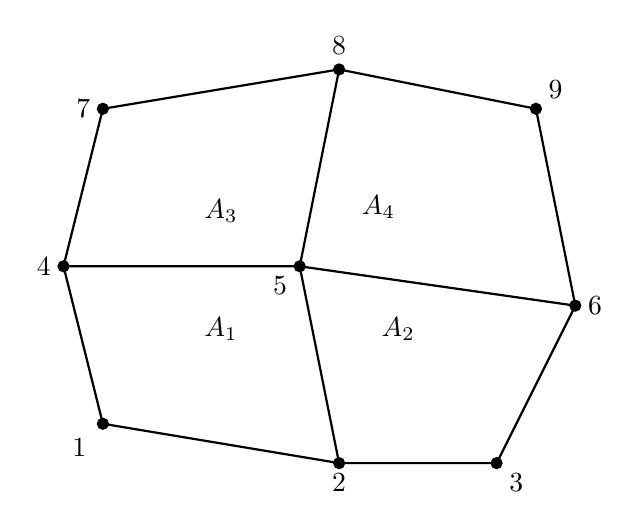
\begin{tikzpicture}
%\draw[fill=gray!5,gray!5](0,0) rectangle (9,7);
%\draw[step=0.5cm,gray,very thin] (0,0) grid (9,7); %background grid
\draw[thick](1.5,1.5) -- (4.5,1) -- (6.5,1) -- (7.5,3) -- (7,5.5) -- (4.5,6) --(1.5,5.5) -- (1,3.5) -- cycle;  
\draw[thick](4.5,1)--(4,3.5)--(4.5,6);
\draw[thick](1,3.5)--(4,3.5)--(7.5,3);
\draw[black,fill=black] (1.5,1.5) circle (2pt); \node[] at (1.2,1.2){1}; %1
\draw[black,fill=black] (4.5,1)   circle (2pt); \node[] at (4.5,0.75){2}; %2
\draw[black,fill=black] (6.5,1)   circle (2pt); \node[] at (6.75,0.75){3}; %3
\draw[black,fill=black] (1,3.5)   circle (2pt); \node[] at (0.75,3.5){4}; %4
\draw[black,fill=black] (4,3.5)   circle (2pt); \node[] at (3.75,3.25){5}; %5
\draw[black,fill=black] (7.5,3)   circle (2pt); \node[] at (7.75,3){6}; %6
\draw[black,fill=black] (1.5,5.5) circle (2pt); \node[] at (1.25,5.5){7}; %7
\draw[black,fill=black] (4.5,6)   circle (2pt); \node[] at (4.5,6.3){8}; %8
\draw[black,fill=black] (7,5.5)   circle (2pt); \node[] at (7.25,5.75){9}; %9
%\draw[thin,dashed](1,3.5)--(4.5,1)--(7.5,3)--(4.5,6)--cycle;
\node[] at (3,2.7){$A_1$}; %8
\node[] at (5.25,2.7){$A_2$}; %8
\node[] at (5,4.25){$A_4$}; %8
\node[] at (3,4.2){$A_3$}; %8
\end{tikzpicture}
\end{center}
\[
q_5^{(1)} = \frac{1}{4}\sum_{e=1}^4 p_e
\] 

In the codes which rely on the $Q_1 \times P_0$ element, the (elemental) pressure
is simply defined as 
\begin{lstlisting}
p=np.zeros(nel,dtype=np.float64)  
\end{lstlisting}
while the nodal pressure is then defined as\footnote{In virtually all stones $p$
stands for the 'raw' pressure and $q$ stands for its projection onto the velocity mesh.} 
\begin{lstlisting}
q=np.zeros(nnp,dtype=np.float64)  
\end{lstlisting}
The element-to-node algorithm is then simply (in 2D):

\begin{lstlisting}
count=np.zeros(nnp,dtype=np.int32)  
for iel in range(0,nel):
    q[icon[0,iel]]+=p[iel]
    q[icon[1,iel]]+=p[iel]
    q[icon[2,iel]]+=p[iel]
    q[icon[3,iel]]+=p[iel]
    count[icon[0,iel]]+=1
    count[icon[1,iel]]+=1
    count[icon[2,iel]]+=1
    count[icon[3,iel]]+=1
q=q/count
\end{lstlisting}



%----------------------------------------------------------------------
\paragraph{Schemes 2,3}.

{\sl Schemes 2,3} are very similar and are presented in Sani \etal (1981) \cite{sagl81a,sagl81b}.
Scheme 2 uses the areas of the surrounding elements as weights for the arithmetic averaging
while scheme 3 uses the area of the triangles:

\begin{multicols}{2}

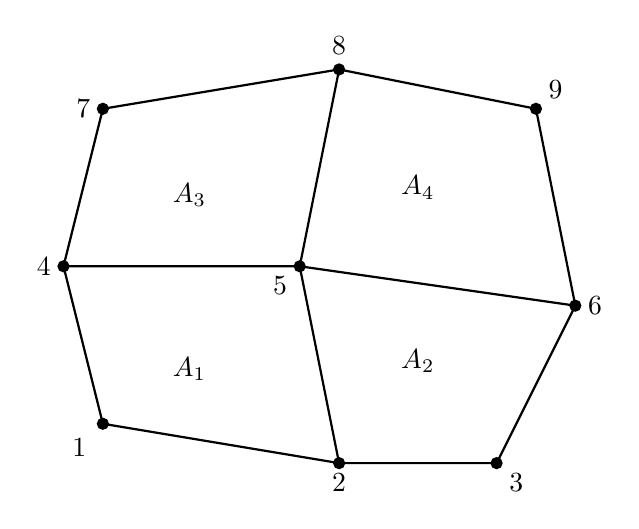
\begin{tikzpicture}
%\draw[fill=gray!5,gray!5](0,0) rectangle (9,7);
%\draw[step=0.5cm,gray,very thin] (0,0) grid (9,7); %background grid
\draw[thick](1.5,1.5) -- (4.5,1) -- (6.5,1) -- (7.5,3) -- (7,5.5) -- (4.5,6) --(1.5,5.5) -- (1,3.5) -- cycle;  
\draw[thick](4.5,1)--(4,3.5)--(4.5,6);
\draw[thick](1,3.5)--(4,3.5)--(7.5,3);
\draw[black,fill=black] (1.5,1.5) circle (2pt); \node[] at (1.2,1.2){1}; %1
\draw[black,fill=black] (4.5,1)   circle (2pt); \node[] at (4.5,0.75){2}; %2
\draw[black,fill=black] (6.5,1)   circle (2pt); \node[] at (6.75,0.75){3}; %3
\draw[black,fill=black] (1,3.5)   circle (2pt); \node[] at (0.75,3.5){4}; %4
\draw[black,fill=black] (4,3.5)   circle (2pt); \node[] at (3.75,3.25){5}; %5
\draw[black,fill=black] (7.5,3)   circle (2pt); \node[] at (7.75,3){6}; %6
\draw[black,fill=black] (1.5,5.5) circle (2pt); \node[] at (1.25,5.5){7}; %7
\draw[black,fill=black] (4.5,6)   circle (2pt); \node[] at (4.5,6.3){8}; %8
\draw[black,fill=black] (7,5.5)   circle (2pt); \node[] at (7.25,5.75){9}; %9
\node[] at (2.6,2.2){$A_1$}; %8
\node[] at (5.5,2.3){$A_2$}; %8
\node[] at (2.6,4.4){$A_3$}; %8
\node[] at (5.5,4.5){$A_4$}; %8
\end{tikzpicture}

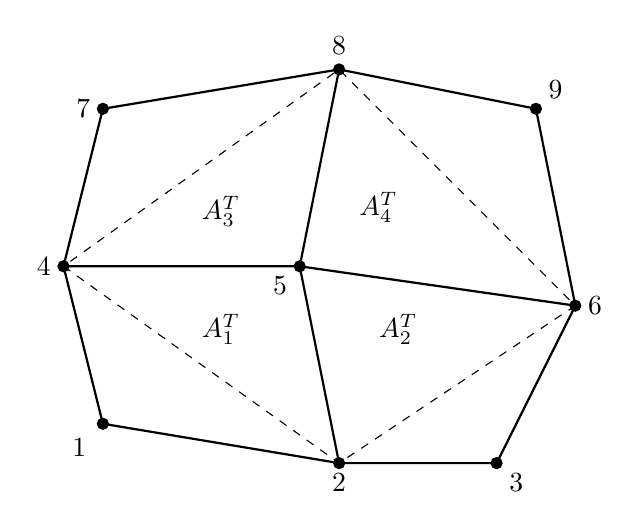
\begin{tikzpicture}
%\draw[fill=gray!5,gray!5](0,0) rectangle (9,7);
%\draw[step=0.5cm,gray,very thin] (0,0) grid (9,7); %background grid
\draw[thick](1.5,1.5) -- (4.5,1) -- (6.5,1) -- (7.5,3) -- (7,5.5) -- (4.5,6) --(1.5,5.5) -- (1,3.5) -- cycle;  
\draw[thick](4.5,1)--(4,3.5)--(4.5,6);
\draw[thick](1,3.5)--(4,3.5)--(7.5,3);
\draw[black,fill=black] (1.5,1.5) circle (2pt); \node[] at (1.2,1.2){1}; %1
\draw[black,fill=black] (4.5,1)   circle (2pt); \node[] at (4.5,0.75){2}; %2
\draw[black,fill=black] (6.5,1)   circle (2pt); \node[] at (6.75,0.75){3}; %3
\draw[black,fill=black] (1,3.5)   circle (2pt); \node[] at (0.75,3.5){4}; %4
\draw[black,fill=black] (4,3.5)   circle (2pt); \node[] at (3.75,3.25){5}; %5
\draw[black,fill=black] (7.5,3)   circle (2pt); \node[] at (7.75,3){6}; %6
\draw[black,fill=black] (1.5,5.5) circle (2pt); \node[] at (1.25,5.5){7}; %7
\draw[black,fill=black] (4.5,6)   circle (2pt); \node[] at (4.5,6.3){8}; %8
\draw[black,fill=black] (7,5.5)   circle (2pt); \node[] at (7.25,5.75){9}; %9
\draw[thin,dashed](1,3.5)--(4.5,1)--(7.5,3)--(4.5,6)--cycle;
\node[] at (3,2.7){$A_1^T$}; %8
\node[] at (5.25,2.7){$A_2^T$}; %8
\node[] at (5,4.25){$A_4^T$}; %8
\node[] at (3,4.2){$A_3^T$}; %8
\end{tikzpicture}

\end{multicols}




\[
q_5^{(2)} = \frac{\sum\limits_{e=1}^4 A_e p_e}{\sum\limits_{e=1}^4 A_e}
\qquad
\qquad
q_5^{(3)} = \frac{\sum\limits_{e=1}^4 A_e^T p_e}{\sum\limits_{e=1}^4 A_e^T}
\] 


\begin{remark} Although Schemes 1,2,3 are similar, scheme 1 is the simplest and fastest
to implement since the areas of neighbouring elements/triangles are not needed.
\end{remark}

\begin{remark} 
Schemes 1,2,3 are identical if all elements are rectangles of identical dimensions.
\end{remark}




%----------------------------------------------------------------------
\paragraph{Scheme 4} This scheme has been designed by me. 
It resembles the last three ones, but the weighing is in this case different.

Let us consider a 1D problem:
\begin{center}
\includegraphics[width=0.5\linewidth]{images/pressure_smoothing/newalgo.png}
\end{center}

Elemental pressures $p_1$ and $p_2$ corresponding to elements 1 and 2 respectively are known at
locations $x_1$ and $x_2$. The two elements have a different size, characterised in this case
by the distances $d_1$ and $d_2$ to their common edge.

The equation of the line passing through points $(x_1,p_1)$ and $(x_2,p_2)$ is 
\[
p(x)=\frac{p_2-p_1}{x_2-x_1}(x-x_1)+p_1
\]
The $x$ coordinate of the common edge is given by $x=x_1+d_1/2$, 
and since $x_2-x_1=(d_1+d_2)/2$, the 
pressure at this location writes:
\[
p(x_M)= \frac{p_2-p_1}{d_1+d_2}d_1+p_1 = \frac{\frac{p_1}{d_1} + \frac{p_2}{d_2}}{\frac{1}{d_1} + \frac{1}{d_2}}
\]
Extrapolating this formula to 2D, $d_1$ and $d_2$ are in fact the element volumes, so that
\[
q_5^{(4)} = 
\frac{\sum\limits_{j=1}^4 \frac{p_j^e}{A_j^e}}{\sum\limits_{j=1}^4 \frac{1}{A_j^e}}
=
\frac{
\frac{p_1^e}{A_1^e}+
\frac{p_2^e}{A_2^e}+
\frac{p_3^e}{A_3^e}+
\frac{p_4^e}{A_4^e}
}{
\frac{1}{A_1^e}+
\frac{1}{A_2^e}+
\frac{1}{A_3^e}+
\frac{1}{A_4^e}
}\]

There remains a problem, due to the presence of the boundary nodes for which 
the sums present in the above equation do not run up to 4. A boundary
node only has three neighbours and a corner node only two. Additional measures
are required for these nodes. 

\begin{center}
\includegraphics[width=0.5\linewidth]{images/pressure_smoothing/newalgo_corner.png}
\end{center}

The pressure value $p_N$ is obtained as follows:
\[
q_N = \frac{ 
 \frac{p_2^e}   {A_2^e}
+\frac{p_3^e}   {A_3^e}
+\frac{p_{2'}^e}{A_{2'}^e}
+\frac{p_{3'}^e}{A_{3'}^e}
}{
 \frac{1}{A_2^e}
+\frac{1}{A_3^e}
+\frac{1}{A_{2'}^e}
+\frac{1}{A_{3'}^e}
}
\]
The areas and pressures of the mirrored elements 2' and 3' are extrapolated from the areas of elements 2 and 6, and 3 and 7 respectively. 
Likewise the pressure $p_M$ at the corner node is obtained through the pressures of its surrounding elements.


%------------------------------------------------------------------------------
\paragraph{Scheme 5 - Least squares} This scheme is presented (among other places) in Lee \etal (1979)
\cite{legs79}. 
Let us start from the patch of 4 $Q_1$ elements counting 9 nodes: 

\begin{center}
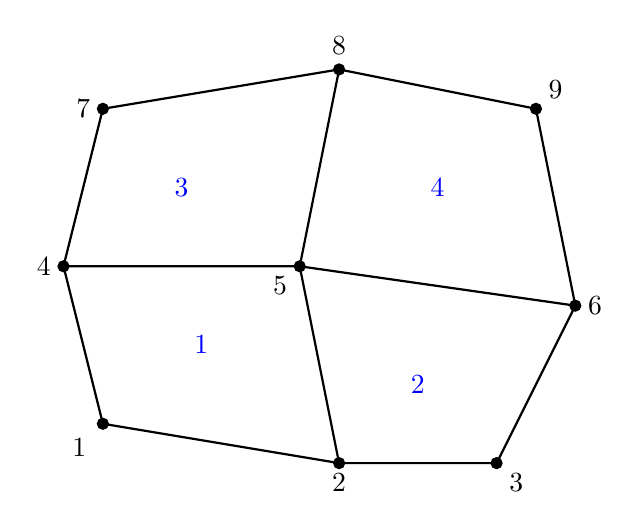
\begin{tikzpicture}
%\draw[fill=gray!5,gray!5](0,0) rectangle (9,7);
%\draw[step=0.5cm,gray,very thin] (0,0) grid (9,7); %background grid
\draw[thick](1.5,1.5) -- (4.5,1) -- (6.5,1) -- (7.5,3) -- (7,5.5) -- (4.5,6) --(1.5,5.5) -- (1,3.5) -- cycle;  
\draw[thick](4.5,1)--(4,3.5)--(4.5,6);
\draw[thick](1,3.5)--(4,3.5)--(7.5,3);

\node[] at (2.75,2.5) {\color{blue}1};
\node[] at (5.5,2) {\color{blue}2};
\node[] at (2.5,4.5) {\color{blue}3};
\node[] at (5.75,4.5) {\color{blue}4};

\draw[black,fill=black] (1.5,1.5) circle (2pt); \node[] at (1.2,1.2){1}; %1
\draw[black,fill=black] (4.5,1)   circle (2pt); \node[] at (4.5,0.75){2}; %2
\draw[black,fill=black] (6.5,1)   circle (2pt); \node[] at (6.75,0.75){3}; %3
\draw[black,fill=black] (1,3.5)   circle (2pt); \node[] at (0.75,3.5){4}; %4
\draw[black,fill=black] (4,3.5)   circle (2pt); \node[] at (3.75,3.25){5}; %5
\draw[black,fill=black] (7.5,3)   circle (2pt); \node[] at (7.75,3){6}; %6
\draw[black,fill=black] (1.5,5.5) circle (2pt); \node[] at (1.25,5.5){7}; %7
\draw[black,fill=black] (4.5,6)   circle (2pt); \node[] at (4.5,6.3){8}; %8
\draw[black,fill=black] (7,5.5)   circle (2pt); \node[] at (7.25,5.75){9}; %9

\end{tikzpicture}
\end{center}



We are looking for a field $q$ living on the nodes.
We build the quantity
\[
J=\iint_\Omega (q-p)^2 dV
\]
where $p$ is the elemental field. To make things clearer we split the integral into 
the sum of elemental integrals:
\[
J=
\iint_{\Omega_1} (q(x,y)-p_1)^2 dV+
\iint_{\Omega_2} (q(x,y)-p_2)^2 dV+
\iint_{\Omega_3} (q(x,y)-p_3)^2 dV+
\iint_{\Omega_4} (q(x,y)-p_4)^2 dV
\]
Inside each element the field $q(x,y)$ is given by a bilinear interpolation so that:
\begin{eqnarray}
J
&=& \iint_{\Omega_1} (\bN_1(x,y) q_1 + \bN_2(x,y)q_2 + \bN_5(x,y)q_5 + \bN_4(x,y)q_4 -p_1)^2 dV \nn\\
&+& \iint_{\Omega_2} (\bN_2(x,y) q_2 + \bN_3(x,y)q_3 + \bN_6(x,y)q_6 + \bN_5(x,y)q_5 -p_2)^2 dV \nn\\
&+& \iint_{\Omega_3} (\bN_4(x,y) q_4 + \bN_5(x,y)q_5 + \bN_8(x,y)q_8 + \bN_7(x,y)q_7 -p_3)^2 dV \nn\\
&+& \iint_{\Omega_4} (\bN_5(x,y) q_5 + \bN_6(x,y)q_6 + \bN_9(x,y)q_9 + \bN_8(x,y)q_8 -p_4)^2 dV 
\end{eqnarray}
where the $N_i$ functions are the basis functions (unusually expressed in $x,y$ coordinates).
The least square procedure looks for the set of $q_i$ such that 
\[
\frac{\partial J}{\partial q_i} =0 \qquad \forall i=1,...9
\]
and this yields 9 equations/constraints for 9 unknowns.
\begin{eqnarray}
\frac{\partial J}{\partial q_1} 
&=& \iint_{\Omega_1} 2 (\bN_1(x,y) q_1 + \bN_2(x,y)q_2 + \bN_5(x,y)q_5 + \bN_4(x,y)q_4 -p_1) \bN_1(x,y) dV \nn\\
\frac{\partial J}{\partial q_2}
&=& \iint_{\Omega_1} 2(\bN_1(x,y) q_1 + \bN_2(x,y)q_2 + \bN_5(x,y)q_5 + \bN_4(x,y)q_4 -p_1) \bN_2(x,y) dV \nn\\
&+& \iint_{\Omega_2} 2(\bN_2(x,y) q_2 + \bN_3(x,y)q_3 + \bN_6(x,y)q_6 + \bN_5(x,y)q_5 -p_2) \bN_2(x,y) dV \nn\\
\frac{\partial J}{\partial q_3}
&=& \iint_{\Omega_2} 2(\bN_2(x,y) q_2 + \bN_3(x,y)q_3 + \bN_6(x,y)q_6 + \bN_5(x,y)q_5 -p_2) \bN_3(x,y) dV \nn\\
\frac{\partial J}{\partial q_4}
&=& \iint_{\Omega_1} 2(\bN_1(x,y) q_1 + \bN_2(x,y)q_2 + \bN_5(x,y)q_5 + \bN_4(x,y)q_4 -p_1) \bN_4(x,y) dV \nn\\
&+& \iint_{\Omega_3} 2(\bN_4(x,y) q_4 + \bN_5(x,y)q_5 + \bN_8(x,y)q_8 + \bN_7(x,y)q_7 -p_3) \bN_4(x,y) dV \nn\\
\frac{\partial J}{\partial q_5}
&=& \iint_{\Omega_1} 2(\bN_1(x,y) q_1 + \bN_2(x,y)q_2 + \bN_5(x,y)q_5 + \bN_4(x,y)q_4 -p_1) \bN_5(x,y) dV \nn\\
&+& \iint_{\Omega_2} 2(\bN_2(x,y) q_2 + \bN_3(x,y)q_3 + \bN_6(x,y)q_6 + \bN_5(x,y)q_5 -p_2) \bN_5(x,y) dV \nn\\
&+& \iint_{\Omega_3} 2(\bN_4(x,y) q_4 + \bN_5(x,y)q_5 + \bN_8(x,y)q_8 + \bN_7(x,y)q_7 -p_3) \bN_5(x,y) dV \nn\\
&+& \iint_{\Omega_4} 2(\bN_5(x,y) q_5 + \bN_6(x,y)q_6 + \bN_9(x,y)q_9 + \bN_8(x,y)q_8 -p_4) \bN_5(x,y) dV \nn\\
\frac{\partial J}{\partial q_6}
&=& \iint_{\Omega_2} 2(\bN_2(x,y) q_2 + \bN_3(x,y)q_3 + \bN_6(x,y)q_6 + \bN_5(x,y)q_5 -p_2) \bN_6(x,y) dV \nn\\
&+& \iint_{\Omega_4} 2(\bN_5(x,y) q_5 + \bN_6(x,y)q_6 + \bN_9(x,y)q_9 + \bN_8(x,y)q_8 -p_4) \bN_6(x,y) dV \nn\\
\frac{\partial J}{\partial q_7}
&=& \iint_{\Omega_3} 2(\bN_4(x,y) q_4 + \bN_5(x,y)q_5 + \bN_8(x,y)q_8 + \bN_7(x,y)q_7 -p_3) \bN_7(x,y) dV \nn\\
\frac{\partial J}{\partial q_8}
&=& \iint_{\Omega_3} 2(\bN_4(x,y) q_4 + \bN_5(x,y)q_5 + \bN_8(x,y)q_8 + \bN_7(x,y)q_7 -p_3) \bN_8(x,y)dV \nn\\
&+& \iint_{\Omega_4} 2(\bN_5(x,y) q_5 + \bN_6(x,y)q_6 + \bN_9(x,y)q_9 + \bN_8(x,y)q_8 -p_4) \bN_8(x,y)dV \nn\\ 
\frac{\partial J}{\partial q_9}
&=& \iint_{\Omega_4} 2(\bN_5(x,y) q_5 + \bN_6(x,y)q_6 + \bN_9(x,y)q_9 + \bN_8(x,y)q_8 -p_4) \bN_9(x,y)dV 
\end{eqnarray}
The factor 2 are removed and the terms $\int p_i N_j $ are known so they end up in the right hand side.
\begin{eqnarray}
 \iint_{\Omega_1} (\bN_1 \bN_1 q_1 + \bN_1 \bN_2 q_2 + \bN_1 \bN_5 q_5 + \bN_1 \bN_4 q_4) dV 
&=& \iint_{\Omega_1} p_1 N_1 dV \nn\\
 \iint_{\Omega_1} (\bN_2 \bN_1 q_1 + \bN_2 \bN_2 q_2 + \bN_2 \bN_5 q_5 + \bN_2 \bN_4 q_4) dV \nn\\
+\iint_{\Omega_2} (\bN_2 \bN_2 q_2 + \bN_3 \bN_2 q_3 + \bN_6 \bN_2 q_6 + \bN_5 \bN_2 q_5) dV 
&=& \iint_{\Omega_1} p_1N_2 dV + \iint_{\Omega_2}  p_2 \bN_2 dV \nn\\
\nn\\
\dots &=& \dots \nn\\
\nn\\
 \iint_{\Omega_4} (\bN_9\bN_5 q_5 + \bN_9\bN_6q_6 + \bN_9\bN_9q_9 + \bN_9\bN_8q_8) dV &=&  \iint_{\Omega_4} p_4 \bN_9 dV 
\end{eqnarray}

The mass matrices corresponding to the four elements are 
\[
{\bm M}_1 = \int_{\Omega_1} \left( \begin{array}{cccc}
 \bN_1 \bN_1 & \bN_1 \bN_2 & \bN_1 \bN_5 & \bN_1 \bN_4 \\
 \bN_2 \bN_1 & \bN_2 \bN_2 & \bN_2 \bN_5 & \bN_2 \bN_4 \\
 \bN_5 \bN_1 & \bN_5 \bN_2 & \bN_5 \bN_5 & \bN_5 \bN_4 \\
 \bN_4 \bN_1 & \bN_4 \bN_2 & \bN_4 \bN_5 & \bN_4 \bN_4 
\end{array}\right) dV
\qquad
{\bm M}_2 = \int_{\Omega_2} \left( \begin{array}{cccc}
 \bN_2 \bN_2 & \bN_2 \bN_3 & \bN_2 \bN_6 & \bN_2 \bN_5 \\
 \bN_3 \bN_2 & \bN_3 \bN_3 & \bN_3 \bN_6 & \bN_3 \bN_5 \\
 \bN_6 \bN_2 & \bN_6 \bN_3 & \bN_6 \bN_6 & \bN_6 \bN_5 \\
 \bN_5 \bN_2 & \bN_5 \bN_3 & \bN_5 \bN_6 & \bN_5 \bN_5 
\end{array}\right) dV
\]
\[
{\bm M}_3 = \int_{\Omega_3} \left( \begin{array}{cccc}
 \bN_4 \bN_4 & \bN_4 \bN_5 & \bN_4 \bN_8 & \bN_4 \bN_7 \\
 \bN_5 \bN_4 & \bN_5 \bN_5 & \bN_5 \bN_8 & \bN_5 \bN_7 \\
 \bN_8 \bN_4 & \bN_8 \bN_5 & \bN_8 \bN_8 & \bN_8 \bN_7 \\
 \bN_7 \bN_4 & \bN_7 \bN_5 & \bN_7 \bN_8 & \bN_7 \bN_7 
\end{array}\right) dV
\qquad
{\bm M}_4 = \int_{\Omega_4} \left( \begin{array}{cccc}
 \bN_5 \bN_5 & \bN_5 \bN_6 & \bN_5 \bN_9 & \bN_5 \bN_8 \\
 \bN_6 \bN_5 & \bN_6 \bN_6 & \bN_6 \bN_9 & \bN_6 \bN_8 \\
 \bN_9 \bN_5 & \bN_9 \bN_6 & \bN_9 \bN_9 & \bN_9 \bN_8 \\
 \bN_8 \bN_5 & \bN_8 \bN_6 & \bN_8 \bN_9 & \bN_8 \bN_8 
\end{array}\right) dV
\]
so that the 9 equations above are actually the result of the assembly process of these four 
elemental systems:
\[
\left( \iint_{\Omega_e} \vec{\bN}^T\vec{\bN} dV \right) \cdot \vec{q}_e = \iint_{\Omega_i} \vec{\bN}^T p_e dV 
\qquad\qquad e=1,2,3,4
\]


%------------------------------------------------------------------------------
\paragraph{Scheme 6 - Consistent pressure recovery}

The is the method presented in Zienkiewicz \& Nakazawa (1982) \cite{zina82}. In the second part 
of this publication the authors wish to establish a simple and effective numerical method to calculate 
variables eliminated by the penalisation process. 
The method involves an additional finite element solution for the nodal pressures using 
the same finite element basis and numerical quadrature as used for the velocity.

Let us start with\footnote{I here voluntarily use $q$ instead of $p$}:
\[
q = -\lambda \vec\nabla\cdot \vec\upnu
\]
We are going to treat this equation as any other PDE in the context of the FE method, i.e. 
we are going to establish its weak form. 
We assume that the pressure is given inside an element by
\[
q(x,y) = \sum_{i=1}^4 \bN_i(x,y) q_i = \vec{\bN} \cdot \vec{q}
\]
and the velocity:
\[
\vec\upnu = (u,v) 
\qquad 
\qquad 
u(x,y)  = \sum_{i=1}^4 \bN_i(x,y) u_i
\qquad 
\qquad 
v(x,y)  = \sum_{i=1}^4 \bN_i(x,y) v_i
\]
where the $\bN_i$ are the $Q_1$ basis functions and $q_i$ are the sought after nodal values. 
We multiply the equation above by a $Q_1$ basis function $\bN_i$ and integrate over the whole domain:
\[
\iint_\Omega \bN_i(x,y) q(x,y) \; dxdy 
= -\lambda \iint_\Omega \bN_i \vec\nabla\cdot \vec\upnu  \; dx dy
\]
As before we now focus on the above expression inside a single element $e$:
\[
\iint_{\Omega_e} \bN_i(x,y) q(x,y) \; dxdy = -\lambda \iint_{\Omega_e} \bN_i \vec\nabla\cdot \vec\upnu \; dx dy
\]
After $\bN_i \rightarrow \vec{\bN}=(\bN_1,\bN_2,\bN_3,\bN_4)^T$, the left hand side term becomes:
\[
\iint _{\Omega_e} \vec{\bN}^T q(x,y) \; dxdy 
=
\iint _{\Omega_e} \vec{\bN}^T \vec{\bN} \cdot \vec{q} \; dxdy 
=
\left(\underbrace{\iint _{\Omega_e} \vec{\bN}^T \vec{\bN} dxdy}_{{\bm M}_e} \right) \cdot \vec{q}  
\]
where ${\bm M}_e$ is the elemental mass matrix.
We now turn to the right hand side. We have
\[
\vec\nabla\cdot \vec\upnu
= \frac{\partial u}{\partial x}+\frac{\partial v}{\partial y}
= \sum_i \frac{\partial \bN_i}{\partial x} u_i + \sum_i \frac{\partial \bN_i}{\partial y} v_i 
\]
We here too define $\vec{V}_e=(u_1,v_1,u_2,v_2,u_3,v_3,u_4,v_4)^T$ so that 

\begin{eqnarray}
&& \iint_{\Omega_e} \vec{\bN} {\vec \nabla}\cdot {\vec \upnu} \; dV \nn\\
&=& \iint_{\Omega_e} \vec{\bN}^T \sum_{i=1}^{4} 
\left( \frac{\partial \bN_i}{\partial x} u_i + \frac{\partial \bN_i}{\partial y} v_i 
\right)  
dV \nonumber\\
&=& 
\iint_{\Omega_e} 
\left(
\begin{array}{c}
\bN_1 \left(
\sum\limits_{i=1}^{4} \frac{\partial \bN_i}{\partial x} u_i +
\sum\limits_{i=1}^{4} \frac{\partial \bN_i}{\partial y} v_i \right) \\
\bN_2 \left(
\sum\limits_{i=1}^{4} \frac{\partial \bN_i}{\partial x} u_i +
\sum\limits_{i=1}^{4} \frac{\partial \bN_i}{\partial y} v_i \right) \\
\bN_3 \left(
\sum\limits_{i=1}^{4} \frac{\partial \bN_i}{\partial x} u_i +
\sum\limits_{i=1}^{4} \frac{\partial \bN_i}{\partial y} v_i \right) \\
\bN_4 \left(
\sum\limits_{i=1}^{4} \frac{\partial \bN_i}{\partial x} u_i +
\sum\limits_{i=1}^{4} \frac{\partial \bN_i}{\partial y} v_i \right) 
\end{array}
\right) dV \nonumber \\  %%%%%%%%%%%%%%%%%%%%%%%%%%
&=& 
\int_{\Omega_e} 
\left(
\begin{array}{ccc}
{\bN}_1& {\bN}_1 &  0 \\\\
{\bN}_2& {\bN}_2 &  0 \\\\
{\bN}_3& {\bN}_3 &  0 \\\\
{\bN}_4& {\bN}_4 &  0 
\end{array}
\right)
\cdot
\left(
\begin{array}{c}
\sum\limits_i \frac{\partial \bN_i}{\partial x} u_i \\ \\
\sum\limits_i \frac{\partial \bN_i}{\partial y} v_i \\ \\
\sum\limits_i (\frac{\partial \bN_i}{\partial y} u_i\! +\! \frac{\partial \bN_i}{\partial x} v_i) 
\end{array}
\right)
\; dV \nonumber\\ %%%%%%%%%%%%%%%%%%%%%%%%%%
&=& 
\int_{\Omega_e} 
\underbrace{
\left(
\begin{array}{cccccc}
{\bN}_1 & {\bN}_1 &  0 \\
{\bN}_2 & {\bN}_2 &  0 \\
{\bN}_3 & {\bN}_3 &  0 \\
{\bN}_4 & {\bN}_4 &  0 
\end{array}
\right)
}_{{\bm N}}
\cdot
\underbrace{
\left(\begin{array}{cccccccc}
\partial_x \bN_1 & 0 &  
\partial_x \bN_2 & 0 &  
\partial_x \bN_3 & 0 &  
\partial_x \bN_4 & 0 \\ \\
0 & \partial_y \bN_1 &   
0 & \partial_y \bN_2 &   
0 & \partial_y \bN_3 &   
0 & \partial_y \bN_4 \\ \\
\partial_y \bN_1 & \partial_x \bN_1 &  
\partial_y \bN_2 & \partial_x \bN_2 &  
\partial_y \bN_3 & \partial_x \bN_3 &  
\partial_y \bN_4 & \partial_x \bN_4 
\end{array}\right)}_{{\bm B}}
\cdot \vec{V}_e
\; dV  \nonumber \\
&=& 
\left(\int_{\Omega_e} {\bm N} \cdot {\bm B} \; dV \right) \cdot \vec{V}_e \nonumber\\
&=& -\G_e^T \cdot {\vec V}_e
\end{eqnarray}

After assembly we arrive at
\[
{\bm M} \cdot \vec{q} = \lambda \G^T \cdot {\vec V} 
\qquad
\text{with}
\qquad
\G_e = -\int_{\Omega_e} {\bm N} \cdot {\bm B} \; dV
\]
where ${\bm M}$ is the global mass matrix, $\vec{q}$ the vector of all 
nodal pressures, $\G$ the discrete gradient matrix and $\vec{V}$
the (velocity) solution vector. 
The system can be easily solved since the mass matrix is a friendly matrix.
The vector ${\vec q}$ contains the nodal pressure values directly, with 
no need for a smoothing scheme! 

\begin{remark}
Very importantly, the mass matrix ${\bm M}$ is to be evaluated at the full integration points, 
while the constraint part (the right hand side of the equation) is to be evaluated at 
the reduced integration point, i.e. in the middle of the element.  
\end{remark}

\begin{remark}
As noted in \cite{zina82}, it is interesting to note that when linear elements are used 
and the lumped matrices are used for the ${\bm M}$ the resulting algebraic equation is identical 
to the smoothing scheme 1 only if a uniform square finite element 
mesh is used. In this respect this method is expected to yield different results when elements 
are not square or even rectangular.
\end{remark}

\begin{remark}
The third column of the matrix ${\bm N}$
and the last line of the ${\bm B}$ matrix could be removed altogether.
If your code is based on the mixed formulation, then you already 
have built matrix $\G$ so you can easily re-use this piece of code 
to compute $\G$ again, this time with a reduced integration quadrature.
If you are using the penalty formulation then you need to program 
all from scratch and then simply do away with these unnecessary terms, or 
you can direcly build the rhs as $\int_{\Omega_e} \vec{\bN}^T p_e$ (assuming
you have previously computed the pressure in the middle of each element 
by means of $p=-\lambda\vec\nabla\cdot\vec\upnu$).
\end{remark}

\begin{remark}
This  scheme is identical to the least square scheme!
\end{remark}


%--------------------------------------------------------------
\paragraph{Scheme 7}

Same as scheme 6, but with lumped mass matrix.  


%--------------------------------------------------------------
\paragraph{Scheme 8 - bilinear interpolation} Let us assume that the centers of the 
four elements make a $Q_1$ quadrilateral element, as shown on this figure:


\begin{center}
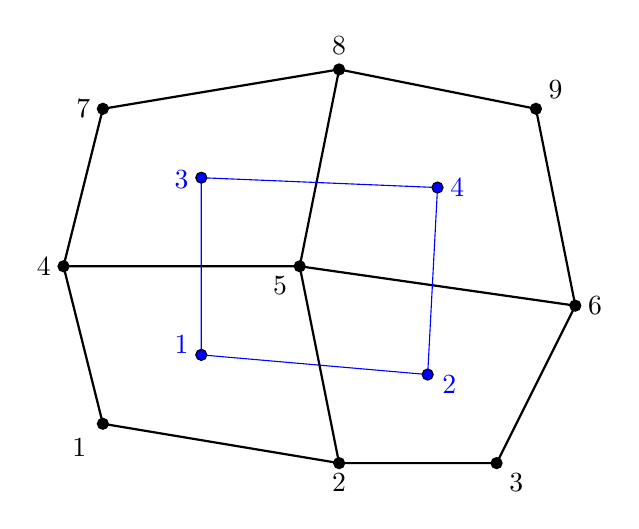
\begin{tikzpicture}
%\draw[fill=gray!5,gray!5](0,0) rectangle (9,7);
%\draw[step=0.5cm,gray,very thin] (0,0) grid (9,7); %background grid
\draw[thick](1.5,1.5) -- (4.5,1) -- (6.5,1) -- (7.5,3) -- (7,5.5) -- (4.5,6) --(1.5,5.5) -- (1,3.5) -- cycle;  
\draw[thick](4.5,1)--(4,3.5)--(4.5,6);
\draw[thick](1,3.5)--(4,3.5)--(7.5,3);

\draw[black,fill=blue] (2.75,2.375) circle (2pt); 
\node[] at (2.5,2.5) {\color{blue}1};
\draw[black,fill=blue] (5.625,2.125) circle (2pt); 
\node[] at (5.9,2) {\color{blue}2};
\draw[black,fill=blue] (5.75,4.5) circle (2pt); 
\node[] at (2.5,4.6) {\color{blue}3};
\draw[black,fill=blue] (2.75,4.625) circle (2pt); 
\node[] at (6,4.5) {\color{blue}4};

\draw[black,fill=black] (1.5,1.5) circle (2pt); \node[] at (1.2,1.2){1}; %1
\draw[black,fill=black] (4.5,1)   circle (2pt); \node[] at (4.5,0.75){2}; %2
\draw[black,fill=black] (6.5,1)   circle (2pt); \node[] at (6.75,0.75){3}; %3
\draw[black,fill=black] (1,3.5)   circle (2pt); \node[] at (0.75,3.5){4}; %4
\draw[black,fill=black] (4,3.5)   circle (2pt); \node[] at (3.75,3.25){5}; %5
\draw[black,fill=black] (7.5,3)   circle (2pt); \node[] at (7.75,3){6}; %6
\draw[black,fill=black] (1.5,5.5) circle (2pt); \node[] at (1.25,5.5){7}; %7
\draw[black,fill=black] (4.5,6)   circle (2pt); \node[] at (4.5,6.3){8}; %8
\draw[black,fill=black] (7,5.5)   circle (2pt); \node[] at (7.25,5.75){9}; %9

\draw[blue](2.75,2.375)--(5.625,2.125)--(5.75,4.5)--(2.75,4.625)--cycle;
\end{tikzpicture}
\end{center}




The values at the corners are $p_1$,
$p_2$, $p_3$ and $p_4$. Assuming that the pressure inside this element can be represented 
by a bilinear field, we have 
\[
p(x,y)= a+ bx +cy +dxy
\]
where the coefficients will be determined by ensuring that $p(x_i,y_i)=p_i$ for $i=1,2,3,4$, or:
\begin{eqnarray}
a+bx_1+cy_1+dx_1y_1 &=& p_1 \\
a+bx_2+cy_2+dx_2y_2 &=& p_2 \\
a+bx_3+cy_3+dx_3y_3 &=& p_3 \\
a+bx_4+cy_4+dx_4y_4 &=& p_4 
\end{eqnarray}
i.e.
\[
\left(
\begin{array}{cccc}
1 & x_1 & y_1 & x_1y_1 \\
1 & x_2 & y_2 & x_2y_2 \\
1 & x_3 & y_3 & x_3y_3 \\
1 & x_4 & y_4 & x_4y_4
\end{array}
\right)\cdot
\left(
\begin{array}{c}
a \\b\\c\\d
\end{array}
\right)
=
\left(
\begin{array}{c}
p_1\\p_2\\p_3\\p_4
\end{array}
\right)
\]

There remains an issue with nodes which are on the boundaries of the domain. These are of course not 
'surrounded' by four pressure values so the above algorithm does not apply directly. However, looking 
at the above figure, and assuming that node 1 is a lower left corner of a 2D domain, we can use the 
bilinear interpolation based on elements 1,2,3,4 to extrapolate a nodal pressure value at node 1. 
The same would apply for nodes 2 and 4 for example. 

\begin{remark}
This scheme is not applicable to quadtree-based meshed.
\end{remark}





\newpage %-----------------------------------------------------------------------------------------
\newpage %-----------------------------------------------------------------------------------------
\section{The value of the timestep}\label{ss:cfl} The chosen time step dt used for time integration is chosen to
comply with the Courant-Friedrichs-Lewy condition \cite{cfd_anderson}.
\begin{equation}
\delta t = C \min \left( \frac{h}{\max |{\bm v}|} , \frac{h^2}{\kappa}  \right)
\end{equation}
where $h$ is a measure of the element size, $\kappa = k/ \rho C_p$ 
is the thermal diffusivity and C is the so-called CFL number chosen in $[0,1[$.

In essence the CFL condition arises when solving hyperbolic PDEs \index{hyperbolic PDE}.
It limits the time step in many explicit time-marching computer simulations
so that the simulation does not produce incorrect results. 

This condition is not needed when solving the Stokes equation but it is mandatory 
when solving the heat transport equation or any kind of advection-diffusion equation. 
Note that any increase of grid resolution (i.e. $h$ becomes smaller) yields an automatic 
decrease of the time step value.






 %------------------------------------
\newpage %-----------------------------------------------------------------------------------------
\section{Exporting data to vtk/vtu format} 
This format seems to be the universally accepted format for 2D and 3D visualisation in 
Computational Geodynamics. Such files can be opened with free softwares such as 
Paraview \footnote{https://www.paraview.org/}, MayaVi \footnote{https://docs.enthought.com/mayavi/mayavi/}
or Visit \footnote{https://wci.llnl.gov/simulation/computer-codes/visit/}.

Unfortunately it is my experience that no simple tutorial exists about how to build 
such files. There is an official document which describes the vtk 
format\footnote{https://www.vtk.org/wp-content/uploads/2015/04/file-formats.pdf}
but it delivers the information in a convoluted way. I therefore describe hereafter 
how \fieldstone{} builds the vtk files. 

I hereunder show vtk file corresponding to the 3x2 grid presented earlier \ref{subsection_meshes}.
In this particular example there are:
\begin{itemize}
\item 12 nodes and 6 elements
\item 1 elemental field: the pressure {\tt p})
\item 2 nodal fields: 1 scalar (the smoothed pressure {\tt q}), 1 vector (the velocity field {\tt u,v,0})
\end{itemize}
Note that vtk files are inherently 3D so that even in the case of a 2D simulation the $z$-coordinate 
of the points and for instance their $z$-velocity component must be provided.
The file, usually called {\sl solution.vtu} starts with a header:

\lstinputlisting[language=python,firstline=1,lastline=3]{images/vtk/solution.vtu}

We then proceed to write the node coordinates as follows:

\lstinputlisting[language=python,firstline=4,lastline=19]{images/vtk/solution.vtu}

These are followed by the elemental field(s):

\lstinputlisting[language=python,firstline=20,lastline=29]{images/vtk/solution.vtu}

Nodal quantities are written next:

\lstinputlisting[language=python,firstline=30,lastline=59]{images/vtk/solution.vtu}

To these informations we must append 3 more datasets. The first one is the connectivity, 
the second one is the offsets and the third one is the type. The first one is trivial
since said connectivity is needed for the Finite Elements. The second must be understood as follows:
when reading the connectivity information in a linear manneer the offset values 
indicate the beginning of each element (omitting the zero value). The third simply is the type of element 
as given in the vtk format document (9 corresponds to a generic quadrilateral with an 
internal numbering consistent with ours). 

\lstinputlisting[language=python,firstline=60,lastline=85]{images/vtk/solution.vtu}

The file is then closed with

\lstinputlisting[language=python,firstline=86,lastline=88]{images/vtk/solution.vtu}

The {\sl solution.vtu} file can then be opened with ParaView, MayaVi or Visit and the reader 
is advised to find tutorials online on how to install and use these softwares. 



 %------------------------------
\newpage %-----------------------------------------------------------------------------------------
\section{Error measurements and convergence rates} \index{$L_1$ norm}
\index{$L_2$ norm}
\index{$H^1$ norm}

What follows is written in the case of a two-dimensional model. Generalisation to
3D is trivial. What follows is mostly borrowed from \cite{thmk14}.

When measuring the order of accuracy of the primitive variables $\vec{v}$ and $p$,
it is standard to report errors in both the $L_1$ and the $L_2$ norm.
For a scalar quantity $\Psi$, the $L_1$ and $L_2$ norms are computed as
\[
\norm{\Psi}_1 = \int_V |\Psi| dV
\quad\quad
\quad\quad
\norm{\Psi}_2 = \sqrt{ \int_V \Psi^2 dV }
\]
For a vector quantity $\vec{k}=(k_x,k_y)$ in a two-dimensional space,
the $L_1$ and $L_2$ norms are defined as:
\[
\norm{\vec{k}}_1 = \int_V (|k_x|+|k_y|) dV
\quad\quad
\quad\quad
\norm{\vec{k}}_2 = \sqrt{ \int_V (k_x^2+k_y^2) dV }
\]
To compute the respective norms
the integrals in the above norms can be approximated by splitting them
into their element-wise contributions. The element volume integral can then
be easily computed by numerical integration using Gauss-Legendre quadrature.

The respective $L_1$ and $L_2$ norms for the pressure error can be evaluated via
\[
e_p^h|_1 = \sum_{i=1}^{n_e} \sum_{q=1}^{n_q} |e_p^h(\vec{r}_q)| w_q |J_q|
\quad\quad
\quad\quad
e_p^h|_2=\sqrt{ \sum_{i=1}^{n_e} \sum_{q=1}^{n_q} |e_p^h(\vec{r}_q)|^2 w_q |J_q| }
\]
where $e_p^h(\vec{r}_q)=p^h(\vec{r}_q) - p(\vec{r}_q)$ 
is the pressure error evaluated at the $q$-th quadrature associated with
the $i$th element. $n_e$ and $n_q$ refer to the number of elements and
the number of quadrature points per element.
$w_q$ and $J_q$ are the quadrature weight of the Jacobian associated with
point $q$.

The velocity error $e_{\vec v}^h$ is evaluated using the following two norms
\[
e_{\vec{v}}^h|_1 = \sum_{i=1}^{n_e} \sum_{q=1}^{n_q} [ |e_u^h(\vec{r}_q)| + |e_v^h(\vec{r}_q)| ]    w_q |J_q|
\quad\quad
\quad\quad
e_{\vec v}^h|_2=\sqrt{ \sum_{i=1}^{n_e} \sum_{q=1}^{n_q} \left[ |e_u^h({\bm r}_q)|^2 +  e_v^h({\bm r}_q)|^2 \right] w_q |J_q| }
\]
where $e_u^h(\vec{r}_q)=u^h(\vec{r}_q) - u(\vec{r}_q)$ and $e_v^h(\vec{r}_q)=v^h(\vec{r}_q)-v(\vec{r}_q)$.




\index{$H^1(\Omega)$ space} \index{$H^1$ norm} \index{$H^1$ semi-norm}
Another norm is very varely used in the geodynamics literature but is preferred in the 
Finite Element literature: the so-called $H^1$ norm. The mathematical basis for this
norm and the nature of the $H^1(\Omega)$ Hilbert space is to be found in many FE books \cite{dohu03,john16,hugh}.
This norm is expression is expressed as follows for a function $f$ such that $f,|\nabla f|\in L^2(\Omega)$
\footnote{\url{https://en.wikipedia.org/wiki/Sobolev_space}}
\[
\norm{f}_{H^1} = \left( \int_\Omega ( |f|^2 + |\nabla f|^2  ) d\Omega   \right)^{1/2}
\]
We then have 
\[
e_{\vec v}^h|_{H^1} = \norm{\vec{v}^h-\vec{v}}_{H^1} = \sqrt{
\sum\limits_{i=1}^d 
\int_\Omega  
\left[
({v}_i^h-{v}_i)^2
+
\vec\nabla(v_i^h-v_i)\cdot\vec\nabla(v_i^h-v_i) 
\right] d\Omega   
}
\]
where $d$ is the number of dimensions.
Note that sometimes the following semi-norm is used \cite{dobo04,bodg06}:
\[
e_{\vec v}^h|_{H^1} = \norm{\vec{v}^h-\vec{v}}_{H^1} = \sqrt{
\sum\limits_{i=1}^d 
\int_\Omega  
\left[
\vec\nabla(v_i^h-v_i)\cdot\vec\nabla(v_i^h-v_i) 
\right] d\Omega   
}
\]
 

When computing the different error norms for $e_p$ and $e_{\vec v}$ for a set of numerical experiments with
varying resolution $h$ we expect the error norms to follow the following relationships:
\[
e_{\vec v}^h|_1 = C h^{rvL_1} 
\quad\quad\quad\quad
e_{\vec v}^h|_2 = C h^{rvL_2} 
\quad\quad\quad\quad 
e_{\vec v}^h|_{H^1} = C h^{rvH^1}
\]
\[
e_p^h|_1 = C h^{rpL_1} 
\quad\quad\quad 
e_p^h|_2 = C h^{rpL_2}
\]
where $C$ is a resolution-independent constant
and $rpXX$ and $rvXX$ are the convergence rates for
pressure and velocity in various norms, respectively. 
Using linear regression on the logarithm of the respective error norm and the resolution $h$,
one can compute the convergence rates of the numerical solutions.

As mentioned in \cite{dobo04}, when finite element solutions converge at
the same rates as the interpolants we say that the method is optimal, i.e.:
\index{optimal rate}

\[
e_{\vec v}^h|_{L_2} = {\cal O}(h^3)
\quad\quad\quad\quad
e_{\vec v}^h|_{H^1} = {\cal O}(h^2)
\quad\quad\quad\quad
e_{p}^h|_{L_2} = {\cal O}(h^2)
\]

%\begin{itemize}
%\item For $Q_1P_0$, the theoretical lower bound for $r_v'$ is 2 and for $r_p'$ it is 1
%\item For $Q_2P_{-1}$, the theoretical lower bound for $r_v'$ is 3 and for $r_p'$ it is 2
%\end{itemize}
We note that when using discontinuous pressure space
(e.g., $P_0$, $P_{-1}$), these bounds remain valid even
when the viscosity is discontinuous provided that the element boundaries conform to the discontinuity.

 
\subsubsection{About extrapolation}
\index{Extrapolation}

{\it Section contributed by W. Bangerth and part of Thieulot \& Bangerth [in prep.]}

In a number of numerical benchmarks we
want to estimate the error $X_h-X^\ast$ between a quantity $X_h$ computed
from the numerical solution $\vec{u}_h,p_h$ and the corresponding value
$X$ computed from the exact solution $\vec{u},p$. Examples of such quantities
$X$ are the root mean square velocity $v_{rms}$, but it could also be a mass flux
across a boundary, an average horizontal velocity at the top boundary, or
any other scalar quantity.

If the exact solution is known, then one can of course compute $X$ from it.
On the other hand, we would of course like to assess convergence also in
cases where the exact solution is not known. In that case, one can compute
an \textit{estimate} $X^\ast$ for $X$ by way of \textit{extrapolation}.
To this end, we make the assumption that asymptotically, $X_h$ converges to
$X$ at a fixed (but unknown) rate $r$, so that
\begin{equation}
  \label{eq:extrapolation-1}
  e_h=|X_h-X| \approx C h^r.
\end{equation}
Here, $X$, $C$ and $r$ are all unknown constants to be determined, although
we are not really interested in $C$.
We can evaluate $X_h$ from the numerical solution
on successively refined meshes with mesh sizes $h$, $h/2$, and $h/4$. Then,
in addition to \eqref{eq:extrapolation-1} we also have
\begin{eqnarray}
  \label{eq:extrapolation-2}
  e_{h/2}=|X_{h/2}-X| \approx C \left(\frac h2\right)^r,
  \\
  \label{eq:extrapolation-3}
  e_{h/4} =|X_{h/4}-X| \approx C \left(\frac h4\right)^r.
\end{eqnarray}
Taking ratios of equations \eqref{eq:extrapolation-1}--\eqref{eq:extrapolation-3},
and replacing the unknown $X$ by an \textit{estimate} $X^\ast$, we then
arrive at the following equation:
\begin{equation*}
\frac{|X_h-X^\star|}{|X_{h/2}-X^\star|}
=
\frac{|X_{h/2}-X^\star|}{|X_{h/4}-X^\star|}=2^r.
\end{equation*}
If one assumes that $X_h$ converges to $X$ uniformly either from above or
below (rather than oscillate around $X$), then this equation allows us
to solve for $X^\ast$ and $r$:
\begin{equation*}
X^\star = \frac{X_h X_{h/2}-X_{h/2}^2}{X_h - 2 X_{h/2} + X_{h/4}}, \qquad\qquad
r = \log_2 \frac{X_{h/2}-X^\star}{X_{h/4}-X^\star}.
\end{equation*}
In the determination of $r$, we could also have used $X_h$ and $X_{h/2}$,
but using $X_{h/2}$ and $X_{h/4}$ is generally more reliable because
the higher order terms we have omitted in \eqref{eq:extrapolation-1} are less
visible on finer meshes.

 %--------------------------------
\newpage %-----------------------------------------------------------------------------------------
\section{The initial temperature field} \subsubsection{Single layer with imposed temperature b.c.}

Let us take a single layer of material characterised by
a heat capacity $c_p$, a heat conductivity $k$
and a heat production term $H$.

\begin{center}
\includegraphics[width=5cm]{images/initial_temperature/tempcond.png}
\end{center}

The Heat transport equation writes
\[
\rho c_p ( \frac{\partial T}{\partial t} + {\vec v} \cdot {\vec \nabla} { T}) = 
{\vec \nabla} \cdot (k {\vec \nabla} T) + \rho H
\]
At steady state and in the absence of a velocity field, and assuming
that the material properties to be independent of time and space, and that
there is no heat production ($H=0$), this equation
simplifies to
\[
\Delta T =0 
\]
Assuming the layer to be parallel to the $x$-axis, this yields to write
\[
T(x,y)=T(y)=\alpha T+ \beta
\]
In order to specify the constants $\alpha$ and $\beta$, we need two constraints.

At the bottom of the layer $y=y_b$ a temperature $T_b$ is prescribed while a temperature
$T_t$ is prescribed at the top with $y=y_t$. This ultimately yields a temperature field in
the layer given by
\[
\boxed{
T(y) = \frac{T_t-T_b}{y_t-y_b}(y-y_b) + T_b
}
\]

If now the heat production coefficient is not zero, the differential equation
reads
\[
 k \Delta T + H = 0 
\]
The temperature field is then expected to be of the form
\[
T(y)= - \frac{H}{2k} y^2 + \alpha y + \beta 
\]
Supplied again with the same boundary conditions, this leads to
\[
\beta=T_b + \frac{H}{2k} y_b^2 - \alpha y_b
\]
ie,
\[
T(y) = -\frac{H}{2k} (y^2-y_b^2) + \alpha (y-y_b) + T_b
\]
and finally
\[
\alpha =  \frac{T_t-T_b}{y_t-y_b}  + \frac{H}{2k}(y_b+y_t)
\]
or,
\[
T(y) = -\frac{H}{2k} (y^2-y_b^2) + \left( \frac{T_t-T_b}{y_t-y_b}  + \frac{H}{2k}(y_b+y_t)   \right) (y-y_b) + T_b
\]

Taking $H=0$ in this equation obviously yields the temperature field obtained previously.
Taking $k=2.25$, $T_t=0C$, $T_b=550C$, $y_t=660km$, $y_b=630km$ yields the following
temperature profiles and heat fluxes when the heat production $H$ varies:
\begin{center}
\includegraphics[width=5cm]{images/initial_temperature/temperature1.pdf}
\includegraphics[width=5cm]{images/initial_temperature/heatflux1.pdf}
\end{center}
Looking at the values at the top, which are somewhat estimated to be
about $55-65mW/m^2$ \cite[table 8.6]{jama}, one sees that value $H=0.8e-6$ yields a very acceptable
heat flux.
Looking at the bottom, the heat flux is then about $0.03W/m^2$
which is somewhat problematic since the heat flux at the Moho
is reported to be somewhere between 10 and 20 $mW/m^2$ in \cite[table 7.1]{jama}.


%-----------------------------------------------------
\subsection{Single layer with imposed heat flux b.c.}

Let us now assume that heat fluxes are imposed at the top and bottom of the layer:
\begin{center} 
\includegraphics[width=5cm]{images/initial_temperature/tempcond2.png}
\end{center}

We start again from the ODE
\[
k \Delta T + H = 0 
\]
but only integrate it once:
\[
k \frac{dT}{dy}  + H y + \alpha  = 0 
\]
At the bottom $q=k(dT/dy)|_{y=y_b} = q_b$ and at the top
$q=k(dT/dy)|_{y=y_t} = q_t$ so that 

\todo[inline]{to finish}


 
%-----------------------------------------------------
\subsection{Single layer with imposed heat flux and temperature b.c. }

\begin{center}
\includegraphics[width=5cm]{images/initial_temperature/tempcond3.png}
\end{center}

\todo[inline]{to finish}


%---------------------------------------------------------------
\subsubsection{Half cooling space}

%---------------------------------------------------------------
\subsubsection{Plate model}

%---------------------------------------------------------------
\subsubsection{McKenzie slab}










 %------------------------------
\newpage %-----------------------------------------------------------------------------------------
\section{The consistent boundary flux (CBF) \label{ss:cbf}} The Consistent Boundary Flux technique was devised to 
alleviate the problem of the accuracy of primary variables 
derivatives (mainly velocity and temperature) on boundaries, 
where basis function (nodal) derivatives do not exist.
These derivatives are important since they are needed to compute
the heat flux (and therefore the NUsselt number) or 
dynamic topography and geoid. 


The idea was first introduced in \cite{mizu86} and later used 
in geodynamics \cite{zhgh93}. It was finally implemented 
in the CitcomS code \cite{zhmt08} and more recently
in the ASPECT code (dynamic topography postprocessor).
Note that the CBF should be seen as a post-processor step 
as it does not alter the primary variables values.

The CBF method is implemented and used in \ref{f_XX}.

%---------------------------------------------------------------
\subsubsection{applied to the Stokes equation}
We start from the strong form:
\[
{\bm \nabla}\cdot{\bm \sigma} = {\bm b}
\]
and then write the weak form:
\[
\int_\Omega N {\bm \nabla}\cdot{\bm \sigma} dV = \int_\Omega N {\bm b} dV
\]
where $N$ is any test function. We then use the two equations:
\[
\bm \nabla \cdot ( N  \bm \sigma ) = N \bm \nabla \cdot \bm \sigma + \bm \nabla N \cdot  \bm \sigma  
\quad\quad \text{(chain rule)}
\]
\[
\int_\Omega (\bm \nabla \cdot \bm f )\; dV = \int_\Gamma \bm f\cdot \bm n \; dS
\quad\quad \text{(divergence theorem)}
\]
Integrating the first equation over $\Omega$ and using the second, we can write:
\[
\int_\Gamma N {\bm \sigma}\cdot {\bm n} \; dS 
-  \int_\Omega {\nabla N} \cdot{\bm \sigma} \; dV 
= \int_\Omega N {\bm b} dV
\]
On $\Gamma$, the traction vector is given by ${\bm t}={\bm \sigma}\cdot {\bm n}$: 
\[
\int_\Gamma N {\bm t} dS =  \int_\Omega {\nabla N} \cdot{\bm \sigma} dV + \int_\Omega N {\bm b} dV
\]
Considering the traction vector as an unknown living on the nodes on the boundary, 
we can expand (for $Q_1$ elements)
\[
t_x = \sum_{i=1}^2 t_{x|i} N_i 
\quad\quad
t_y = \sum_{i=1}^2 t_{y|i} N_i 
\]
on the boundary so that the left hand term yields a mass matrix $M'$.
Finally, using our previous experience of discretising the weak form, we can write:
\[
M' \cdot {\cal T} = -\K {\cal V} - \G {\cal P} + f
\]
where ${\cal T}$ is the vector of assembled tractions which we want to compute 
and ${\cal V}$ and ${\cal T}$ are the solutions of the Stokes problem. 
Note that the assembly
only takes place on the elements along the boundary.

Note that the assembled mass matrix is tri-diagonal can be easily solved with 
a Conjugate Gradient method. With a trapezoidal integration rule 
(i.e. Gauss-Lobatto) the matrix can even be diagonalised and the resulting 
matrix is simply diagonal, which results in a very cheap solve \cite{zhgh93}.

%---------------------------------------------------------------
\subsubsection{applied to the heat equation}
We start from the strong form of the heat transfer equation (without the source terms for simplicity):
\[
\rho c_p
\left(\frac{\partial T}{\partial t} + {\bm v}\cdot {\bm \nabla}T\right)
=
{\bm \nabla} \cdot k{\bm \nabla T}
\]
The weak form then writes:
%\[
%\int_\Omega N
%\rho c_p
%\left(\frac{\partial T}{\partial t} + {\bm v}\cdot {\bm \nabla}T\right) dV
%=
%\int_\Omega N
%{\bm \nabla} \cdot k{\bm \nabla T} dV
%\]
\[
\int_\Omega N
\rho c_p
\frac{\partial T}{\partial t} dV 
+
\rho c_p
\int_\Omega N
 {\bm v}\cdot {\bm \nabla}T  dV
=
\int_\Omega N
{\bm \nabla} \cdot k{\bm \nabla T} dV
\]
Using once again integration by parts and divergence theorem:
\[
\int_\Omega N
\rho c_p
\frac{\partial T}{\partial t} dV 
+
\rho c_p
\int_\Omega N
 {\bm v}\cdot {\bm \nabla}T  dV
=
\int_\Gamma N k {\bm \nabla T} \cdot {\bm n} d\Gamma
-
\int_\Omega  {\bm \nabla} N \cdot k{\bm \nabla T} dV
\]
On the boundary we are interested in the heat flux ${\bm q}=-k {\bm \nabla T}$
\[
\int_\Omega N
\rho c_p
\frac{\partial T}{\partial t} dV 
+
\rho c_p
\int_\Omega N
 {\bm v}\cdot {\bm \nabla}T  dV
=
-\int_\Gamma N {\bm q} \cdot {\bm n} d\Gamma
- \int_\Omega  {\bm \nabla} N \cdot k{\bm \nabla T} dV
\]
or,
\[
\int_\Gamma N {\bm q} \cdot {\bm n} d\Gamma
=
-\int_\Omega N
\rho c_p
\frac{\partial T}{\partial t} dV 
-\rho c_p
\int_\Omega N
 {\bm v}\cdot {\bm \nabla}T  dV
- \int_\Omega  {\bm \nabla} N \cdot k{\bm \nabla T} dV
\]
Considering the normal heat flux $q_n = {\bm q} \cdot {\bm n}$ as an unknown 
living on the nodes on the boundary, 
\[
q_n = \sum_{i=1}^2 q_{n|i} N_i
\]
so that the left hand term becomes a mass matrix for the shape functions living on 
the boundary.
We have already covered the right hand side terms when building the FE system 
to solve the heat transport equation, so that in the end 
\[
M' \cdot {\cal Q}_n =
- M \cdot \frac{\partial \bm T}{\partial t} -K_a \cdot {\bm T} - K_d \cdot {\bm T} 
\]
where ${\cal Q}_n$ is the assembled vector of normal heat flux components.
Note that in all terms the assembly only takes place over the elements along the boundary.







\newpage
What follows only applies to the reference element.

\begin{verbatim}
    N
 3-----2
 |     |
W|     |E
 |     |
 0-----1
    S
\end{verbatim}

We start from 
\begin{eqnarray}
\int_{\Gamma} N_i {\bm t} dS 
&=& 
 \int_{\Gamma_{0-1}} N_i {\bm t} dS  
+\int_{\Gamma_{1-2}} N_i {\bm t} dS  
+\int_{\Gamma_{2-3}} N_i {\bm t} dS  
+\int_{\Gamma_{3-0}} N_i {\bm t} dS
\end{eqnarray}
for $i=0,3$. Let us start with $N_0$, then 

\begin{eqnarray}
\int_{\Gamma} N_0 {\bm t} dS 
&=& 
 \int_{\Gamma_{0-1}} N_0 {\bm t} dS  
+\int_{\Gamma_{1-2}} N_0 {\bm t} dS  
+\int_{\Gamma_{2-3}} N_0 {\bm t} dS  
+\int_{\Gamma_{3-0}} N_0 {\bm t} dS \nn\\
&=& \int_{\Gamma_{0-1}} N_0 (N_0^\Gamma {\bm t}_0 + N_1^\Gamma {\bm t}_1) dS \nn\\ 
&+& \int_{\Gamma_{1-2}} N_0 (N_1^\Gamma {\bm t}_1 + N_2^\Gamma {\bm t}_2) dS \nn\\
&+& \int_{\Gamma_{2-3}} N_0 (N_2^\Gamma {\bm t}_2 + N_3^\Gamma {\bm t}_3) dS \nn\\
&+& \int_{\Gamma_{3-0}} N_0 (N_3^\Gamma {\bm t}_3 + N_0^\Gamma {\bm t}_0) dS \nn\\ 
&=& \left( \int_{\Gamma_{0-1}} N_0 N_0^\Gamma dS \right) {\bm t}_0 + \left( \int_{\Gamma_{0-1}} N_0 N_1^\Gamma dS\right) {\bm t}_1 \nn\\ 
&+& \left( \int_{\Gamma_{1-2}} N_0 N_1^\Gamma dS \right) {\bm t}_1 + \left( \int_{\Gamma_{1-2}} N_0 N_2^\Gamma dS\right) {\bm t}_2 \nn\\
&+& \left( \int_{\Gamma_{2-3}} N_0 N_2^\Gamma dS \right) {\bm t}_2 + \left( \int_{\Gamma_{2-3}} N_0 N_3^\Gamma dS\right) {\bm t}_3 \nn\\
&+& \left( \int_{\Gamma_{3-0}} N_0 N_3^\Gamma dS \right) {\bm t}_3 + \left( \int_{\Gamma_{3-0}} N_0 N_0^\Gamma dS\right) {\bm t}_0 \nn  
\end{eqnarray}

In what follows we will make use of 
\[
\int_{-1}^{+1} \frac{1}{4} (1-x)(1-x) dx = 2/3 
\]
\[
\int_{-1}^{+1} \frac{1}{4} (1+x)(1+x) dx = 2/3 
\]
\[
\int_{-1}^{+1} \frac{1}{4} (1+x)(1-x) dx = 1/3 
\]



\newpage 
\begin{eqnarray}
\int_{\Gamma_{0-1}} N_0(r,s=-1) N_0^\Gamma(r) dS  &=&  \int_{-1}^{+1}\frac{1}{2}(1-r) \cdot  \frac{1}{2}(1-r) dr= 2/3 \nn\\
\int_{\Gamma_{0-1}} N_0(r,s=-1) N_1^\Gamma(r) dS  &=&  \int_{-1}^{+1}\frac{1}{2}(1-r) \cdot  \frac{1}{2}(1+r) dr= 1/3 \nn\\
\int_{\Gamma_{1-2}} N_0(r=+1,s) N_1^\Gamma(s) dS  &=&  \int_{-1}^{+1}\frac{1}{4}(0)(1-s) \cdot  \frac{1}{2}(1-s) ds=0 \nn\\
\int_{\Gamma_{1-2}} N_0(r=+1,s) N_2^\Gamma(s) dS  &=&  \int_{-1}^{+1}\frac{1}{4}(0)(1-s) \cdot  \frac{1}{2}(1+s) ds=0 \nn\\
\int_{\Gamma_{2-3}} N_0(r,s=+1) N_2^\Gamma(r) dS  &=&  -\int_{-1}^{+1}\frac{1}{4}(1-r)(0) \cdot  \frac{1}{2}(1+r) dr=0 \nn\\
\int_{\Gamma_{2-3}} N_0(r,s=+1) N_3^\Gamma(r) dS  &=&  -\int_{-1}^{+1}\frac{1}{4}(1-r)(0) \cdot  \frac{1}{2}(1-r) dr=0 \nn\\
\int_{\Gamma_{3-0}} N_0(r=-1,s) N_3^\Gamma(s) dS  &=&  -\int_{-1}^{+1}\frac{1}{2}(1-s) \cdot  \frac{1}{2}(1+s) ds= -1/3 \nn\\
\int_{\Gamma_{3-0}} N_0(r=-1,s) N_0^\Gamma(s) dS  &=&  -\int_{-1}^{+1}\frac{1}{2}(1-s) \cdot  \frac{1}{2}(1-s) ds= -2/3 \nn
\end{eqnarray}

\begin{eqnarray}
\int_{\Gamma_{0-1}} N_1(r,s=-1) N_0^\Gamma(r) dS  &=&  \int_{-1}^{+1} \frac{1}{2}(1+r)     \cdot  \frac{1}{2}(1-r) dr= 1/3\nn\\
\int_{\Gamma_{0-1}} N_1(r,s=-1) N_1^\Gamma(r) dS  &=&  \int_{-1}^{+1} \frac{1}{2}(1+r)     \cdot  \frac{1}{2}(1+r) dr= 2/3\nn\\
\int_{\Gamma_{1-2}} N_1(r=+1,s) N_1^\Gamma(s) dS  &=&  \int_{-1}^{+1} \frac{1}{2}(1-s)     \cdot  \frac{1}{2}(1-s) ds= 2/3\nn\\
\int_{\Gamma_{1-2}} N_1(r=+1,s) N_2^\Gamma(s) dS  &=&  \int_{-1}^{+1} \frac{1}{2}(1-s)     \cdot  \frac{1}{2}(1+s) ds= 1/3\nn\\
\int_{\Gamma_{2-3}} N_1(r,s=+1) N_2^\Gamma(r) dS  &=&  -\int_{-1}^{+1}\frac{1}{4}(1+r)(0)  \cdot  \frac{1}{2}(1+r) dr= 0\nn\\
\int_{\Gamma_{2-3}} N_1(r,s=+1) N_3^\Gamma(r) dS  &=&  -\int_{-1}^{+1}\frac{1}{4}(1+r)(0)  \cdot  \frac{1}{2}(1-r) dr= 0\nn\\
\int_{\Gamma_{3-0}} N_1(r=-1,s) N_3^\Gamma(s) dS  &=&  -\int_{-1}^{+1}\frac{1}{4}(0)(1-s)  \cdot  \frac{1}{2}(1+s) ds= 0\nn\\
\int_{\Gamma_{3-0}} N_1(r=-1,s) N_0^\Gamma(s) dS  &=&  -\int_{-1}^{+1}\frac{1}{4}(0)(1-s)  \cdot  \frac{1}{2}(1-s) ds= 0\nn
\end{eqnarray}

\begin{eqnarray}
\int_{\Gamma_{0-1}} N_2(r,s=-1) N_0^\Gamma(r) dS  &=&  \int_{-1}^{+1} \frac{1}{4}(1+r)(0)  \cdot  \frac{1}{2}(1-r) dr= 0\nn\\
\int_{\Gamma_{0-1}} N_2(r,s=-1) N_1^\Gamma(r) dS  &=&  \int_{-1}^{+1} \frac{1}{4}(1+r)(0)  \cdot  \frac{1}{2}(1+r) dr= 0\nn\\
\int_{\Gamma_{1-2}} N_2(r=+1,s) N_1^\Gamma(s) dS  &=&  \int_{-1}^{+1} \frac{1}{2}(1+s)     \cdot  \frac{1}{2}(1-s) ds= 1/3 \nn\\
\int_{\Gamma_{1-2}} N_2(r=+1,s) N_2^\Gamma(s) dS  &=&  \int_{-1}^{+1} \frac{1}{2}(1+s)     \cdot  \frac{1}{2}(1+s) ds= 2/3 \nn\\
\int_{\Gamma_{2-3}} N_2(r,s=+1) N_2^\Gamma(r) dS  &=&  -\int_{-1}^{+1}\frac{1}{2}(1+r)     \cdot  \frac{1}{2}(1+r) dr= -2/3\nn\\
\int_{\Gamma_{2-3}} N_2(r,s=+1) N_3^\Gamma(r) dS  &=&  -\int_{-1}^{+1}\frac{1}{2}(1+r)     \cdot  \frac{1}{2}(1-r) dr= -1/3\nn\\
\int_{\Gamma_{3-0}} N_2(r=-1,s) N_3^\Gamma(s) dS  &=&  -\int_{-1}^{+1}\frac{1}{4}(0)(1+s)  \cdot  \frac{1}{2}(1+s) ds= 0\nn\\
\int_{\Gamma_{3-0}} N_2(r=-1,s) N_0^\Gamma(s) dS  &=&  -\int_{-1}^{+1}\frac{1}{4}(0)(1+s)  \cdot  \frac{1}{2}(1-s) ds= 0\nn
\end{eqnarray}

\begin{eqnarray}
\int_{\Gamma_{0-1}} N_3(r,s=-1) N_0^\Gamma(r) dS  &=&  \int_{-1}^{+1} \frac{1}{4}(1-r)(0) \cdot  \frac{1}{2}(1-r) dr= 0\nn\\
\int_{\Gamma_{0-1}} N_3(r,s=-1) N_1^\Gamma(r) dS  &=&  \int_{-1}^{+1} \frac{1}{4}(1-r)(0) \cdot  \frac{1}{2}(1+r) dr= 0\nn\\
\int_{\Gamma_{1-2}} N_3(r=+1,s) N_1^\Gamma(s) dS  &=&  \int_{-1}^{+1} \frac{1}{4}(0)(1+s) \cdot  \frac{1}{2}(1-s) ds= 0\nn\\
\int_{\Gamma_{1-2}} N_3(r=+1,s) N_2^\Gamma(s) dS  &=&  \int_{-1}^{+1} \frac{1}{4}(0)(1+s) \cdot  \frac{1}{2}(1+s) ds= 0\nn\\
\int_{\Gamma_{2-3}} N_3(r,s=+1) N_2^\Gamma(r) dS  &=&  -\int_{-1}^{+1}\frac{1}{2}(1-r)    \cdot  \frac{1}{2}(1+r) dr= -1/3\nn\\
\int_{\Gamma_{2-3}} N_3(r,s=+1) N_3^\Gamma(r) dS  &=&  -\int_{-1}^{+1}\frac{1}{2}(1-r)    \cdot  \frac{1}{2}(1-r) dr= -2/3\nn\\
\int_{\Gamma_{3-0}} N_3(r=-1,s) N_3^\Gamma(s) dS  &=&  -\int_{-1}^{+1}\frac{1}{2}(1+s)    \cdot  \frac{1}{2}(1+s) ds= -2/3\nn\\
\int_{\Gamma_{3-0}} N_3(r=-1,s) N_0^\Gamma(s) dS  &=&  -\int_{-1}^{+1}\frac{1}{2}(1+s)    \cdot  \frac{1}{2}(1-s) ds= -1/3\nn
\end{eqnarray}







\newpage
so finally
\begin{eqnarray}
\int_{\Gamma} N_0 {\bm t} dS &=& \frac{1}{3} {\bm t}_1 -  \frac{1}{3} {\bm t}_3  \nn\\ 
\int_{\Gamma} N_1 {\bm t} dS &=& \frac{1}{3} {\bm t}_0 + \frac{4}{3} {\bm t}_1 +  \frac{1}{3} {\bm t}_2 \nn\\   
\int_{\Gamma} N_2 {\bm t} dS &=& \frac{1}{3} {\bm t}_1  -\frac{1}{3}  {\bm t}_3\nn\\ 
\int_{\Gamma} N_3 {\bm t} dS &=& -\frac{1}{3} {\bm t}_0 - \frac{1}{3} {\bm t}_2 - \frac{4}{3} {\bm t}_3 \nn
\end{eqnarray}
 
\[
\frac{1}{3}
\left(
\begin{array}{cccccccc}
. &. &1 &. &. &. &-1 & .\\
.& . &. &1 &. &. &. &-1 \\
1 & . & 4 & . & 1 &. & .& .\\
. &1 & . & 4 & . & 1 &. & . \\
. & . & 1 & .& . & . & -1 & .\\
. & . & . & 1 & .& . & . & -1 \\
-1 & . & . & . & -1 & .  & -4 & . \\
. & -1 & . & . & . & -1 & .  & -4  
\end{array}
\right)
\cdot
\left(
\begin{array}{c}
t_{x,0}\\
t_{y,0}\\
t_{x,1}\\
t_{y,1}\\
t_{x,2}\\
t_{y,2}\\
t_{x,3}\\
t_{y,3}
\end{array}
\right)
=
\left(
\begin{array}{c}
\\
\\
\\
rhs\\
\\
\\
\\
\end{array}
\right)
\]
Note that the resulting matrix is symmetric.


\newpage
Let us start with a small example, a 3x2 element FE grid:

\begin{center}
\begin{verbatim}
8=======9======10======11
|       |       |       |
|  (3)  |  (4)  |  (5)  |
|       |       |       |
4=======5=======6=======7
|       |       |       |
|  (0)  |  (1)  |  (2)  |
|       |       |       |
0=======1=======2=======3
\end{verbatim}
\end{center}


\begin{eqnarray}
\text{Element 0:} \quad\quad
\int_{\Gamma} N_i {\bm t} dS 
&=& \int_{\Gamma_{0-1}} N_i {\bm t} dS  +\int_{\Gamma_{1-5}} N_i {\bm t} dS +\int_{\Gamma_{5-4}} N_i {\bm t} dS  +\int_{\Gamma_{4-0}} N_i {\bm t} dS\\
\text{Element 1:} \quad\quad
\int_{\Gamma} N_i {\bm t} dS 
&=& \int_{\Gamma_{1-2}} N_i {\bm t} dS  +\int_{\Gamma_{2-6}} N_i {\bm t} dS +\int_{\Gamma_{6-5}} N_i {\bm t} dS  +\int_{\Gamma_{5-1}} N_i {\bm t} dS\\
\text{Element 2:} \quad\quad
\int_{\Gamma} N_i {\bm t} dS 
&=& \int_{\Gamma_{2-3}} N_i {\bm t} dS  +\int_{\Gamma_{3-7}} N_i {\bm t} dS +\int_{\Gamma_{7-6}} N_i {\bm t} dS  +\int_{\Gamma_{6-2}} N_i {\bm t} dS\\
\text{Element 3:} \quad\quad
\int_{\Gamma} N_i {\bm t} dS 
&=& \int_{\Gamma_{4-5}} N_i {\bm t} dS  +\int_{\Gamma_{5-9}} N_i {\bm t} dS +\int_{\Gamma_{9-8}} N_i {\bm t} dS  +\int_{\Gamma_{8-4}} N_i {\bm t} dS\\
\text{Element 4:} \quad\quad
\int_{\Gamma} N_i {\bm t} dS 
&=& \int_{\Gamma_{5-6}} N_i {\bm t} dS  +\int_{\Gamma_{6-10}} N_i {\bm t} dS +\int_{\Gamma_{10-9}} N_i {\bm t} dS  +\int_{\Gamma_{9-5}} N_i {\bm t} dS\\
\text{Element 5:} \quad\quad
\int_{\Gamma} N_i {\bm t} dS 
&=& \int_{\Gamma_{6-7}} N_i {\bm t} dS  +\int_{\Gamma_{7-11}} N_i {\bm t} dS +\int_{\Gamma_{11-10}} N_i {\bm t} dS  +\int_{\Gamma_{10-6}} N_i {\bm t} dS
\end{eqnarray}

We see that the integral $\int_{\Gamma_{1-5}} N_i {\bm t} dS$ of element 0 is exactly the opposite\footnote{these are line integrals, one is going from node 1 to 5, the other from 5 to 1} of the the integral $\int_{\Gamma_{5-1}} N_i {\bm t} dS$ of element 1, so that their contributions to the assembled matrix 
would actually cancel out. Likewise, any edge common to two elements will see in the expressions above two integrals of opposite sign, shich ultimately will not
contribute to the assembled matrix. 

Let us then remove the integrals over edges 1-5, 2-6, 4-5, 5-6, 6-7, 5-9 and 6-10 off the equations above:

\begin{eqnarray}
\text{Element 0:} \quad\quad
\int_{\Gamma} N_i {\bm t} dS 
&=& \int_{\Gamma_{0-1}} N_i {\bm t} dS  +\int_{\Gamma_{4-0}} N_i {\bm t} dS\\
&=& \int_{\Gamma_{0-1}} N_i (N_0 {\bm t}_0 + N_1 {\bm t}_1)  dS  +\int_{\Gamma_{4-0}} N_i (N_0 {\bm t}_0 +N_4 {\bm t}_4) dS\\
&=& \int_{\Gamma_{0-1}} N_i N_0 dS \quad {\bm t}_0  +  \int_{\Gamma_{0-1}} N_i N_1 dS \quad  {\bm t}_1  
+\int_{\Gamma_{4-0}} N_i N_0 dS \quad  {\bm t}_0 + \int_{\Gamma_{4-0}} N_i N_4 dS \quad {\bm t}_4 \nonumber\\
\text{Element 1:} \quad\quad
\int_{\Gamma} N_i {\bm t} dS 
&=& \int_{\Gamma_{1-2}} N_i {\bm t} dS  \\ 
&=& \int_{\Gamma_{1-2}} N_i (N_1 {\bm t}_1 + N_2 {\bm t}_2) dS  \\ 
\text{Element 2:} \quad\quad
\int_{\Gamma} N_i {\bm t} dS 
&=& \int_{\Gamma_{2-3}} N_i {\bm t} dS  +\int_{\Gamma_{3-7}} N_i {\bm t} dS \\ 
\text{Element 3:} \quad\quad
\int_{\Gamma} N_i {\bm t} dS 
&=& \int_{\Gamma_{9-8}} N_i {\bm t} dS  +\int_{\Gamma_{8-4}} N_i {\bm t} dS\\
\text{Element 4:} \quad\quad
\int_{\Gamma} N_i {\bm t} dS 
&=& \int_{\Gamma_{10-9}} N_i {\bm t} dS \\ 
&=& \int_{\Gamma_{10-9}} N_i (N_{10}{\bm t}_{10}+N_{9}{\bm t}_9) dS \\ 
\text{Element 5:} \quad\quad
\int_{\Gamma} N_i {\bm t} dS 
&=& \int_{\Gamma_{7-11}} N_i {\bm t} dS +\int_{\Gamma_{11-10}} N_i {\bm t} dS  
\end{eqnarray}
We see that the 






























\end{document}




 %--------------------------
\newpage %-----------------------------------------------------------------------------------------
\section{Computing gradients - the recovery process \label{ss:gradrecovery}} 
write about recovering accurate strain rate components and heat flux components on the nodes.

Let $\vec g(\vec r)$  be the desired nodal 
field which we want to be the continuous $Q_1$ representation of the field $\vec \nabla f^h$.
Since the derivative of the shape function does not exist on the nodes we need to design
an algorithm do do so. This problem is well known and has been 
investigated %\cite{XX.XXX}
\improvement{refs!}.
The main standard techniques are listed hereafter.


%..............................
\subsubsection{Global recovery}

The global recovery approach is rather simple: we wish to find $\vec g^h$
such that it satisfies
\[
\int_\Omega \phi \vec g^h \; d\Omega  = \int_\Omega \phi \vec\nabla f^h \; d\Omega 
\quad\quad \forall \phi
\] 
We will then successively replace $\phi$ by all the shape functions $N_i$ 
and since we have $g^h=\sum_j N_i g_i$ we then obtain
\[
\sum_j \int N_i N_j d\Omega g_i = \int N_i  \vec\nabla f^h \; d\Omega 
\]
or, 
\[
\mathbb{M} \cdot \vec{\cal G} = \vec f
\]



%..................................................
\subsubsection{Local recovery - centroid average over patch}





%..................................................
\subsubsection{Local recovery - nodal average over patch}

Let $j$ be the node at which we want to compute $\vec g$.
Then 
\[
\vec g_j = \vec g(\vec r_j) = 
\frac{\sum\limits_{ e \text{ adj. to }j} |\Omega_e| (\vec\nabla f)_e(\vec r_j) }{\sum |\Omega_e|}
\]
where $|\Omega_e|$ is the volume of the element and $(\vec\nabla f^h)_e(\vec r_j)$
is the gradient of $f$ as obtained with the shape functions inside element $e$ and 
computed at location $\vec r_j$.

%........................................................
\subsubsection{Local recovery - least squares over patch}



%........................................................
\subsubsection{Link to pressure smoothing}

When the penalty method is used to solve the Stokes equation, the pressure
is then given by $p=-\lambda \vec\nabla \cdot \vec v$. As explained in 
section \ref{sec_penalty}, the velocity is first obtained and the pressure 
is recovered by using this equation as a postprocessing step. Since the divergence 
cannot be computed easily at the nodes, the pressure is traditionally computed 
in the middle of the elements, yielding an elemental pressure field (remember, 
we are talking about $Q_1P_0$ elements here -- bi/tri-linear velocity, discontinuous
constant pressure)



\improvement{tie to fieldstone 12}

 %----
\newpage %-----------------------------------------------------------------------------------------
\section{Static condensation} \index{general}{Static Condensation}

The idea behind static condensation is quite simple: in some cases, there are dofs 
belonging to an element which only belong to that element. For instance, the so-called MINI 
element ($P_1^+ \times P_1$) showcases a bubble function in the middle (see section \ref{ss:pair}). 
In the following, $\vec{\cal V}^\star$ corresponds to the list of such dofs inside an element.
The discretised Stokes equations on any element looks like:

\begin{equation}
\left(
\begin{array}{ccc}
\K   & L & \G \\
L^T & \K^\star  & H \\
\G^T & H^T & 0
\end{array}
\right)_e
\left(
\begin{array}{c}
\vec{\cal V} \\ \vec{\cal V}^\star \\ \vec{\cal P}
\end{array}
\right)_e
=
\left(
\begin{array}{c}
\vec{f} \\ \vec{f}^\star \\ \vec{h}
\end{array}
\right)_e
\end{equation}
This is only a re-writing of the elemental Stokes matrix where the matrix $\K$ has been 
split in four parts.
Note that the matrix $\K^\star$ is diagonal.\todo{check}

This can also be re-written in non-matrix form:
\begin{eqnarray}
\K \cdot \vec{\cal V} + L \cdot \vec{\cal V}^\star + \G \cdot \vec{\cal P} &=& \vec{f} \\
L^T V + K^\star \cdot  \vec{\cal V}^\star + H \cdot \vec{\cal P} &=& \vec{f}^\star \\
\G^T \cdot \vec{\cal V} + H^T \vec{\cal V}^\star &=& \vec{h}
\end{eqnarray}
The $\vec{\cal V}^\star$ in the second equation can be isolated:
\[
\vec{\cal V}^\star = \K^{-\star} \cdot ( \vec{f}^\star - L^T \cdot \vec{\cal V} - H \cdot \vec{\cal P})
\]
and inserted in the first and third equations:
\begin{eqnarray}
\K \cdot \vec{\cal V} + L \left[ \K^{-\star} ( \vec{f}^\star - L^T \cdot \vec{\cal V} - H \cdot \vec{\cal P} )  \right] + \G \cdot \vec{\cal P} &=& \vec{f} \\
\G^T \cdot \vec{\cal V} + H^T \left[  \K^{-\star} ( \vec{f}^\star - L^T \cdot \vec{\cal V} - H \cdot \vec{\cal P}) \right]  &=& \vec{h}
\end{eqnarray}
or,
\begin{eqnarray}
(\K-L\cdot \K^{-\star} \cdot L^T)\cdot \vec{\cal V} + (G-L\cdot \K^{-\star} \cdot H) \cdot \vec{\cal P} &=& \vec{f}-L\cdot \K^{-\star} \cdot \vec{f}^\star \\
(G^T -H^T\cdot \K^{-\star}\cdot  L^T ) \cdot \vec{\cal V}  - 
(H^T \cdot \K^{-\star} \cdot H )\cdot \vec{\cal P}   &=& \vec{h} -H^T\cdot \K^{-\star}\cdot \vec{f}^\star
\end{eqnarray}
i.e.
\begin{eqnarray}
\underline{\K} \cdot \vec{\cal V} + \underline{\G}\cdot \vec{\cal P} &=& \underline{\vec{f}} \\
\underline{\G}^T \cdot \vec{\cal V} - \underline{\C} \cdot \vec{\cal P} &=& \underline{\vec{h}}
\end{eqnarray}
with
\begin{eqnarray}
\underline{\K}&=& K-L\cdot \K^{-\star} \cdot L^T \\
\underline{\G}&=& G-L\cdot \K^{-\star} \cdot H \\
\underline{\C}&=& H^T \cdot \K^{-\star} \cdot H \\
\underline{\vec{f}}&=& \vec{f}-L\cdot \K^{-\star} \cdot \vec{f}^\star \\
\underline{\vec{h}}&=& \vec{h} -H^T\cdot \K^{-\star}\cdot \vec{f}^\star
\end{eqnarray}
Note that $\underline{\K}$ is symmetric, and so is the Stokes matrix.


For instance, in the case of the MINI element, the dofs corresponding to the bubble 
could be eliminated at the elemental level, which would make the Stokes matrix smaller
(see book by Braess \cite{braess}). 
However, it is then important to note that static condensation introduces a 
pressure-pressure term which was not there in the original formulation.









 %----------------------------------------
\newpage %-----------------------------------------------------------------------------------------
\section{Measuring incompressibility \label{ss_incomp}} 
The velocity divergence error integrated over the whole element is given by
\begin{equation}
e_{div}= \int_\Omega (\vec\nabla\cdot \vec v^h - \underbrace{\vec\nabla\cdot \vec v}_{=0}  ) \; d\Omega
= \int_\Omega (\vec\nabla\cdot \vec v^h) \; d\Omega
\end{equation}
where $\Gamma_e$ is the boundary of element $e$ and $\vec{n}$ is the unit 
outward normal of $\Gamma_e$.

Furthermore we also have \cite{dobo04}:
\[
e_{div}
= \int_{\Gamma_e} \vec{v}^h\cdot\vec{n} \;  d\Gamma
\]
The reason is as follows and is called the divergence theorem:
suppose a volume $V$ subset of $\mathbb{R}^d$ which is compact
and has a piecewise smooth boundary $S$, and if $\vec F$ is
a continuously differentiable vector field then
\[
\int_V ( \vec\nabla\cdot\vec F)\; dV = \int_S (\vec F \cdot \vec n)\; dS
\]
The left side is a volume integral while the right side is a surface integral.
Note that sometimes the notation $d\vec S = \vec n \; dS $ is used so that 
$\vec F \cdot \vec n \; dS = \vec F \cdot d\vec S$.

The average velocity divergence over an element can be defined as 
\[
<\vec \nabla \cdot \vec v>_e 
= \frac{1}{V_e} \int_{\Omega_e}  (\vec\nabla\cdot\vec v) \; d\Omega
= \frac{1}{V_e} \int_{\Gamma_e} \vec{v}\cdot\vec{n} \; d\Gamma
\]
Note that for elements using discontinuous pressures we shall 
recover a zero divergence element per element (local mass conservation)
while for continuous pressure elements the mass conservation 
is guaranteed only globally (i.e. over the whole domain), see section 3.13.2 of \cite{grsa}.

Note that one could instead compute $<|\vec\nabla\cdot \vec v|>_e$. Either volume or 
surface integral can be computed by means of an appropriate Gauss-Legendre quadrature algorithm.

\improvement[inline]{implement and report}


 %---------------------------
\newpage %-----------------------------------------------------------------------------------------
\section{Parallel or not?} \label{sec:parallel} \index{general}{Domain Decomposition}

%---------------------------
\subsubsection{Rationale}

Let us assume that we want ro run a simulation of the whole Earth mantle
with a constant resolution of $5\text{km}$. The volume of the mantle is
\[
V_{mantle}=\frac{4}{3}\pi (R_{out}^3-R_{in}^3) \simeq  10^{12}  km^3
\]
while the volume of an element is $V_{e} = 125 \text{km}^3$ (this is 
only an average since the tesselation of a hollow sphere with 
hexahedra yields elements which are not all similar \cite{thie18}).
Consequently, the number of cells needed to discretise the mantle
is 
\[
N_{el}=\frac{V_{mantle}}{V_{e}}\simeq 8\times 10^9
\]
We know that the matrix size is approx. 4 times the number of elements in 3D:
\[
N\simeq 25 \times 10^9
\]
Using between 9 and 125 particles per element (a very conservative number),
the total number of particles is then
\[
N_{particles}  \geq 10^{10}
\]
The unescapable conclusion is that high-resolution 3D 
calculations 
 have a very large memory footprint and require extremely long computational times.

The only way to overcome this problem is by resorting to 
using supercomputers with many processors and large memory capacities.

The idea behind parallel programming is to have each processor carry out 
only a subset of the total number of operations required. In order to reduce 
the memory footprint on each processor, only a subset of the computational
mesh is known by each: one speaks then of domain decomposition.

An example of such a large parallel calculation of 3D convection with 
domain decomposition in a spherical shell can be found in \cite{krhb12}:

\begin{center}
a)\includegraphics[width=7cm]{images/parallel/krhb2}
b)\includegraphics[width=7cm]{images/parallel/krhb1} \\
{\captionfont a)Isocontours of the temperature field; b) Partitioning of the domain onto 512 proc. 
The mesh counts 1,424,176 cells. The solution has approximately 54 million unknowns 
(39 million vel., 1.7 million press., and 13 million temp.)
}
\end{center}


\Literature:
\begin{itemize}
\item Three parallel iterative solvers for the Stokes system, discretized by low order 
tetrahedral elements, are compared with respect to their numerical efficiency and their 
scalability running on up to 786,432 parallel threads. Gmeiner et al (2016) \cite{gmhj16}
\end{itemize}


%----------------------------------------------
\subsubsection{Strong scaling vs weak scaling}

\begin{center}
\includegraphics[width=16cm]{images/parallel/fig}
\end{center}


 %------------------------------
\newpage %-----------------------------------------------------------------------------------------
\section{Corner flow} \label{sec:cornerflow} \begin{flushright} {\tiny {\color{gray} cornerflow.tex}} \end{flushright}

The mantle wedge comprised between the downgoing slab and the overriding plate
has been extensively studied since very important geodynamical processes take place
in it or right above it (slab dehydration and water transport, melting, over-riding plate
deformation, vulcanism, ...).

To first approximation one can approach the problem and simplify it greatly by 
assuming that both plates kinematic behaviour are independent of what happens 
in the wedge, that the wedge geometry does not change over time, that the problem 
is essentially 2D, and that the mantle extends very far away from the actual 
wedge (plates are infinite). 

Under such assumptions, it is possible to derive an analytical solution 
for incompressible Stokes flow in the wedge as documented at p. 224 in  Batchelor \cite{batchelor}.

Literature: \cite{tosl78}

\todo[inline]{FIND refs. check new version of Vol7 theoretical geophys}

A corner flow setup is shown hereunder:
\begin{center}
\includegraphics[width=8cm]{images/cornerflow/corner}
\end{center}

\index{general}{Stream Function} \index{general}{Biharmonic Operator}
The solution to this problem is arrived at by means of the stream function $\Phi$, defined 
as $u=-\partial \Phi/\partial y$ and $v=\partial \Phi/partial x$, so that we automatically have $\vec\nabla\cdot\vec\upnu=0$.
As shown in Section~\ref{sec:streamfunction}, the stream function $\Phi$ is then the solution to 
the biharmonic equation
\[
\vec\nabla^2 \vec\nabla^2 \Phi = \vec\nabla^4 \Phi = 0
\]

Considering the geometry of the problem has plates of infinite extent with constant relative
velocity, the solution for velocity everywhere is expected to be independent of $r$. This means the
equation is separable and we will use a solution of the form
\[
\Phi(r,\theta)= R(r) f(\theta)
\]
However, given the infinite extent of the domain, the velocity is expected to be 
independent of $r$, so we postulate $R(r)=r$ (look at the relationship between velocity components and 
stream function), or:
\[
\Phi(r,\theta)= r f(\theta)
\]
and we then have to solve
\[
\Delta \left( \frac{1}{r} (f+f'')\right) = \frac{1}{r^3}(f+2f''+f'''')=0.
\]
The solution of this equation for $f$ is:
\begin{eqnarray}
f(\theta) &=&A \sin\theta + B \cos \theta + C \theta \sin \theta + D \theta \cos \theta   \nn\\
f'(\theta)&=&A \cos\theta - B \sin \theta + C (\sin \theta + \theta \cos \theta) + D (\cos \theta - \theta \sin \theta) \nn
\end{eqnarray}
with
\[
\upnu_r=\frac{1}{r}\frac{\partial \Phi}{\partial \theta} = f'(\theta)
\]
\[
\upnu_\theta=-\frac{\partial \Phi}{\partial r} = -f(\theta)
\]
$A$, $B$, $C$ and $D$ are four constants to be determined by means of the boundary conditions which 
are as follows:
\begin{eqnarray}
\upnu_r(\theta=0)            &=&  0 \nonumber\\
\upnu_\theta(\theta=0)       &=&  0 \nonumber\\
\upnu_r(\theta=\theta_0)     &=&  -U_0 \nonumber\\
\upnu_\theta(\theta=\theta_0)&=&  0 \nonumber
\end{eqnarray}
or,
\begin{eqnarray}
f'(0)= A+D &=& 0 \\
f(0) = B &=& 0 \\
f'(\theta_0) &=& -U_0 \\
f(\theta_0) &=& 0 
\end{eqnarray}

From the second equation it is trivial to see that $B=0$, so that:
\[
f(\theta)=A \sin\theta + C \theta \sin \theta + D \theta \cos \theta
\]
\[
f'(\theta)=A \cos\theta + C (\sin \theta + \theta \cos \theta) + D (\cos \theta - \theta \sin \theta)
\]
From the first one we obtain $D=-A$ so that 
\[
f(\theta)=A (\sin\theta - \theta \cos \theta)  + C \theta \sin \theta 
\]
\[
f'(\theta)=A ( \theta \sin \theta)    + C (\sin \theta + \theta \cos \theta) 
\]
The last two boundary conditions yield:
\[
0=A (\sin\theta_0 - \theta_0 \cos \theta_0)  + C \theta_0 \sin \theta_0 
\]
\[
-U_0 = A ( \theta_0 \sin \theta_0)    + C (\sin \theta_0 + \theta_0 \cos \theta_0) 
\]
or, 
\[
A= - U_0 \frac{\theta_0 \sin\theta_0}{\theta_0^2-\sin^2\theta_0}
\quad\quad
C=   U_0 \frac{\sin\theta_0 - \theta_0 \cos \theta_0}{\theta_0^2-\sin^2\theta_0}
\]
Finally:
\[
(A,B,C,D)=
(
-\theta_0 \sin\theta_0,
0,
\sin\theta_0 - \theta_0 \cos \theta_0,
\theta_0 \sin\theta_0
)
\frac{U_0}{\theta_0^2-\sin^2\theta_0}
\]

We have 
\begin{eqnarray}
{\bm e}_r      &=& \cos\theta {\bm e}_x + \sin\theta {\bm e}_y \\
{\bm e}_\theta &=& -\sin\theta {\bm e}_x + \cos\theta {\bm e}_y
\end{eqnarray}
so that the velocity field can be expressed in Cartesian coordinates:
\begin{eqnarray}
{\bm \upnu} 
&=& \upnu_r {\bm e}_r + \upnu_\theta {\bm e}_\theta \nn\\
&=& \upnu_r ( \cos\theta {\bm u}_x + \sin\theta {\bm e}_y) + \upnu_\theta (-\sin\theta {\bm u}_x + \cos\theta {\bm e}_y) \nn\\
&=& ( \upnu_r \cos\theta - \upnu_\theta \sin\theta  ) {\bm e}_x + ( \upnu_r \sin\theta + \upnu_\theta\cos\theta  ) {\bm e}_y
\end{eqnarray}




\Literature: Ribe \cite{ribe89} present a simple model for the mantle flow induced by back arc spreading behind a subduction zone.



 %-------------------------------
\newpage %-----------------------------------------------------------------------------------------
\section{Surface processes \label{sec:surfaceprocesses}} %.......................................................................
\subsubsection{In 1D - simple nonlinear diffusion a la \cite{bucl97}}

The tectonic-scale transport equations describe long term changes
in topography $h(x,y,t)$ as a result of simultaneous short- and long-range
mass transport processes \cite{befh92,kobe94}.

The short-range surface processes are represented by cumulative effects of hillslope 
processes (soil creep, rainsplash, slides) that remove material from uplifted areas 
down to the valleys. 
It is then assumed that the horizontal material flux $\vec{q}_s$ is related to 
local slope $\vec\nabla h$ by $\vec{q}_s=-K_s \vec{\nabla}h$ 
where $K_s$ is the effective diffusivity. Assumption of conservation of mass 
volume leads to the linear diffusion equation for erosion:
\[
\frac{\partial h}{\partial t} = K_s \Delta h
\]
This equation can be solved with constant-elevation (fixed $h$ value)
boundary conditions simulating local base levels of erosion. 

Note that is practice the coefficient $K_s$ might depend on slope and curvature, 
i.e.
\[
\frac{\partial h}{\partial t} = K_s(x,y,h,\vec\nabla h)\Delta h
\]
Following \cite{goss76}, Burov \& Cloetingh use an empirical non linear 
expression $K_s=k_s(x) (\vec\nabla h)^n$. 




%...........................................................
\subsubsection{In 1D - not so simple, a la \cite{anpa19}}. 

The change in surface elevation rate due to surface processes is equal
to the divergence of the sediment flux 
(assuming there is no density difference between the bedrock and
sediment and ignoring the effects of compaction):
\[
\frac{\partial h}{\partial t} = -\frac{\partial q_s}{\partial x}
\]
where $h$ is the topography, $t$ is the time, $q_s$ represents the sediment flux, 
and $x$ is the horizontal coordinate. 

The next step consists in a formulation for the sediment flux. Still following \cite{anpa19}, 
in the subaerial environment, it is possible to define the sediment transport 
flux $q_s$ in terms of the water flux $q_w$ as
\[
q_s=-(K+c q_w^n) \frac{\partial h}{\partial x}
\]
where $K$ is the slope diffusivity, $c$ is the transport coefficient, 
and $n \geq 1$ is the power law that defines the type
of relationship between the sediment transport and the water flux 
(Simpson \& Schlunegger, 2003; Smith \& Bretherton, 1972).
\todo[inline]{get these papers}
This model accounts for hillslope diffusion processes where the topography will tend to
a dispersive diffusion (Culling, 1960) and fluvial transport processes that result in concentrative diffusion
due to water run off (Graf, 1984). For a simple parameterization we choose a linear relationship between
sediment transport and water flux $(n=1)$.

The water flux can be related to the water discharge/effective rainfall $\alpha$ as
\[
\frac{\partial}{\partial x} (\vec{n} q_w) = -\alpha
\]
where $\vec n$ is a unit vector directed down the surface gradient (Smith \& Bretherton, 1972). 
By assuming a constant $\alpha$ and integrating equation (12) over the surface in the downstream direction, we obtain

\[
q_w = \alpha x_d
\]
where $x_d$ is the downstream distance from the drainage divide. By substituting equations (11) and
(13) into (10) we obtain the 1-D sediment mass conservation equation for combined hillslope and
discharge-dependent fluvial transport
\[
\frac{\partial h}{\partial t} = \frac{\partial}{\partial x} \left( (K+k \alpha x_d) 
\frac{\partial h}{\partial x}   \right)
\]
where the downstream distance $x_d$ is calculated at each time step as the distance from the topographic highs
to the valley floors. Because $q_w$ is dependent on the length of the drainage, the model mimics 1-D landscapes
similar to river profiles in which fluvial processes are dominant.

 %-------------
\newpage %-----------------------------------------------------------------------------------------
\section{Geometric multigrid} 

The following is mostly borrowed from the Wikipedia page on multigrid methods\footnote{\url{https://en.wikipedia.org/wiki/Multigrid_method}}.

There are many types of (geometric) multigrid algorithms, but the common features are that a hierarchy of grids is considered. The important steps are:

\begin{itemize}
\item {\sl Smoothing}: reducing high frequency errors, for example using a few iterations of the Gauss-Seidel method.
\item {\sl Residual Computation}: computing residual error after the smoothing operation(s).
\item {\sl Restriction}: downsampling the residual error to a coarser grid.
\item {\sl Interpolation or prolongation}: interpolating a correction computed on a coarser grid into a finer grid.
\item {\sl Correction}: Adding prolongated coarser grid solution onto the finer grid.
\end{itemize}

There are many choices of multigrid methods with varying trade-offs between speed of solving a single iteration and the rate of convergence with said iteration. The 3 main types are V-Cycle, F-Cycle, and W-Cycle.

Any geometric multigrid cycle iteration is performed on a hierarchy of grids and hence it can be coded using recursion. Since the function calls itself with smaller sized (coarser) parameters, the coarsest grid is where the recursion stops.

Note that the ratio of the number of nodes between two consecutive levels has to be constant between all the levels. Often powers of 2 are used (especially if the grids are based on quad/octrees) but it is not a requirement. 



\begin{center}
\includegraphics[width=6cm]{images/multigrid/mggrid}\\
{\scriptsize Image from \url{http://web.utk.edu/~wfeng1/research.html}}
\end{center}



What follows is a pseudo-code example of a recursive V-Cycle Multigrid for solving 
the Poisson equation ($\nabla^2 \phi = f$) 
on a uniform grid of spacing $h$:

\begin{verbatim}
function phi = V_Cycle(phi,f,h)
% Pre-Smoothing
phi = smoothing(phi,f,h);
% Compute Residual Errors
r = residual(phi,f,h);
% Restriction
rhs = restriction(r);
eps = zeros(size(rhs));
% stop recursion at smallest grid size
if smallest_grid_size_is_achieved
   eps = smoothing(eps,rhs,2*h);
else        
   eps = V_Cycle(eps,rhs,2*h);        
end
% Prolongation and Correction
phi = phi + prolongation(eps);
% Post-Smoothing
phi = smoothing(phi,f,h);    
end
\end{verbatim}

A multigrid method with an intentionally reduced tolerance can be used as an efficient preconditioner for an external iterative solver. The solution may still be obtained in ${\cal O}(N)$ time as well as in the case where the multigrid method is used as a solver. Multigrid preconditioning is used in practice even for linear systems, typically with one cycle per iteration.

\begin{center}
\includegraphics[width=8cm]{images/multigrid/cycles}\\
{\scriptsize Taken from \cite{tack10}: Different types of multigrid cycle with four grid levels: (top left) V-cycle, (top right) W-cycle,
(bottom left) F-cycle and (bottom right) full multigrid. ‘S’ denotes smoothing while ‘E’ denotes
exact coarse-grid solution.}
\end{center} 

Check Kaus BEcker syllabus!

\Literature: \cite{tack10,gery10,mabl15,lopp14,tros01,moma05}
 %-----------------------------------------------------
\newpage %-----------------------------------------------------------------------------------------
\section{Algebraic multigrid} 
\Literature: \cite{nano12}\cite{nota12}
 %-----------------------------------------------------
\newpage %-----------------------------------------------------------------------------------------
\section{Computing depth \label{ss:depth}} 
\begin{flushright} {\tiny {\color{gray} computing\_depth.tex}} \end{flushright}

In the case of a perfectly rectangular, cylindrical or spherical domain, 
computing the depth of any given point inside the domain is trivial. 
However, when the free surface becomes somewhat distorted, the concept of 
depth needs to be refined. What follows is an attempt at bringing clarity
as to how to compute depth in all cases.

The depth $d({\bm r})$ satisfies the equation:
\[
\frac{{\bm g}}{|{\bm g}|} \cdot {\bm \nabla} d = 1
\]
with $d=0$ at the surface.

This is a form of steady-state advection equation (the time derivative is zero, 
there is no diffusion, nor any source term).

Given the boundary conditions, one could solve this equation 
over the whole domain. 

Note that in the case of a cartesian box, ${\bm g}=-g {\bm u}_z$,
we need to solve 
\[
- \frac{\partial}{\partial z} d = 1
\]
For a flat top surface at $d(z=L_z)=0$ so that in the end
\[
d(z)=L_z-z
\]

 %----------------------------
\newpage %-----------------------------------------------------------------------------------------
\section{The Geoid} \label{ss:geoid} 
%---------------------------------
\subsubsection{What is the geoid?}



The geoid is usually defined in two ways:
\begin{itemize}
\item Mean sea level (easy to define in the oceans, but harder on land)
\item A gravitational equipotential surface. This means that everywhere at sea level experiences the same value of gravity potential, so there is no tendency for water to flow downhill since all points in the vicinity have the same value of gravity potential, pointed toward the center of the earth.
\end{itemize}

\begin{center}
\includegraphics[width=10cm]{images/geoid/ww15mgh}\\
{\captionfont Data Max value: 85.4 meters, east of New Guinea. Data Min value:-107.0 meters, south of India. 
This image shows 15'x15' geoid undulations covering the planet Earth from the NIMA/GSFC WGS-84 EGM96 15' Geoid Height File. The undulations refer to the differences from the WGS-84(G873) reference ellipsoid. Map and description from National Geodetic Survey.}
\end{center}
%https://www.usna.edu/Users/oceano/pguth/md_help/geology_course/geoid.htm


%---------------------------------
\subsubsection{How to compute it?}

%---------------------------------
\subsubsection{Interesting modelling}

\begin{center}
\includegraphics[width=15cm]{images/geoid/mogu96}
{\scriptsize Idealized 2D slab calculations for each viscosity model: geoid and geoid filtered 
to pass only the longest wavelengths ($\sim$ 4000 km).
(a) Cold slab extends to 500 km depth in the upper mantle, 
(b) Slab extends to 750 km so that it is partly supported by the high viscosity lower mantle at 670 km. 
(c) Slab tilted at 45\degree to the vertical extending to the top of the lower mantle. 
Taken from \cite{mogu96}}
\end{center}
 %-----------------------------------------------
\newpage %-----------------------------------------------------------------------------------------
\section{Mixing and stirring, the Lyapunov time/exponent}\label{ss:lyapunov}\index{general}{Lyapunov Time}
\begin{flushright} {\tiny {\color{gray} mixing\_stirring.tex}} \end{flushright}

Many approaches are taken in the literature when it comes 
to studying mixing/stirring in fluids, and in our case the mantle.

For example, \textcite{sato12} (2012) 
measure the convective stirring efficiency using two Lagrangian methods: 
the first determines the mixing time associated with
different wavelengths of heterogeneity following the approach of \textcite{feri01} (2001)
The second determines the value of
the maximum Finite Time Lyapunov Exponents (FTLE) as described in 
\textcite{fasa03} (2003), and measures the rate at
which heterogeneities are stretched by mantle motions.

In the review of \textcite{vavt24} by Nicolas Coltice, his review reads:
\begin{displayquote}
{\color{darkgray}
``
The first studies of mantle mixing date back to the 1980’s and one of the 
difficulty was to deal with scales. So 2 approaches were taken: one dealing explicitly 
with scales, such as the authors do here with configurational entropy. It was in 
relationship with the observations of heterogeneities at all scales (marble cake like at 
first, more comprehensive nowadays with mid-ocean ridge heterogeneities etc…). 
The other approach is to work with the theory of dynamic systems, because mantle convection 
is chaotic. The use of Lyapunov exponent characterize the local and global properties of 
stretching of heterogeneities. Mixing happens when an heterogeneity is stretched at a 
scale at which chemical diffusion operates. This scale for the Earth is about 1cm I 
would say (some papers talk about it). Lyapunov exponent are a form of stretching rate 
when mixing is chaotic. Configurational entropy and Lyapunov exponent can be related 
with Ergodicity theory. 
''
}
\end{displayquote}





In \textcite{taxi02} (2002) we read: 

\begin{displayquote}
{\color{darkgray}
``
Two-dimensional simulations of simple mantle convection (\textcite{chri89}, 1989; 
\textcite{ketu90}, 1990; \textcite{scha94}) suggest that for whole-mantle 
convection the mantle should be homogenized in a time-scale of less than 1 Gyr, although
unmixed islands may remain. Non-Newtonian rheology, which is thought to be 
important in the upper mantle \cite{kawu93}, may somewhat inhibit mixing (\textcite{tepy98}, 1998). 
The rate at which blobs of anomalous (e.g. primitive) material are stretched
and assimilated into the flow depends on their relative viscosity; very viscous blobs
can survive intact for many mantle overturns (\textcite{mang96}, 1996).
\\
In three-dimensional geometry with only poloidal flow, mixing may be significantly
less efficient than in two dimensions (\textcite{schh95}, 1995; \textcite{schh96}, 1996) 
but, if the toroidal flow associated with plate motions is 
included (\textcite{gaot91}, 1991), mixing can instead be more efficient 
(\textcite{feri98} (1998)).
\\
High viscosity in the deep mantle is not sufficient to maintain different reservoirs
over geological time-scales (\textcite{feri01}, 2001; van Keken \& Ballentine 1998,
1999), in contrast to predictions from earlier calculations at lower convective vigour
(\textcite{guda86b}, 1986). Part of the reason for this apparent discrepancy is that
the latter study used a kinematically driven flow rather than buoyancy-driven flow.
Since a viscosity jump does not affect densities, thermal buoyancy-driven flow has no
problem crossing it, so substantial mass exchange occurs between upper and lower
mantles. Buoyancy is thus necessary to maintain separate reservoirs.
''
}
\end{displayquote}


In \textcite{gowh06} (2006) we find
\begin{displayquote}
{\color{darkgray}
``
Heterogeneities in a convecting fluid are deformed by
stirring and finally erased by diffusive mixing. Chemical diffusion in mantle rock
acts on the scale of centimetres over the lifetime of the Earth, but our models
resolve km-scales. Therefore this paper deals only with convective stirring. Some
nice studies about mantle stirring and mixing in 2-d have been done (e.g. 
\cite{chri89,guda86b,kest91,ketu90,mebo95,olyb84,olyb84b,teyl96,teyp97,tepy98}).
Unfortunately, results from studies in 2-d can be extrapolated to 3-d only in a limited
manner. Tracers in 3-d poloidal stationary convection move on 2-d toruslike
surfaces. Stirring is constrained to these surfaces. Cross-cell stirring becomes possible
in time-dependent flows, but may not be very efficient \cite{schh96}. Large-scale stirring is
enhanced by a toroidal component, but convectively isolated islands of laminar
stirring may remain \cite{feri98}. Convection in the Earth is time-dependent and the surface
planform shows a strong toroidal component today. Since there is currently no
general understanding about the stirring behaviour of the mantle, a case-by-case
study of different models is necessary.
''
}
\end{displayquote}


\textcite{kest91} (1991) looked into chaotic mixing and state:
\begin{displayquote}
{\color{darkgray}
``
The extent of mixing is quantitatively measured by 
calculating the deformation undergone by passive, elliptical
strain markers. Deformation of a marker is characterized by
its elongation $a/a_0$, where $a$ is the length of the semimajor
axis and $a_0$, is the initial length. For infinitesimal markers,
deformation is controlled by the local flow field and is 
obtained by integrating the strain rate tensor along the particle's 
trajectory \cite{ketu90}. The aspect ratio $\epsilon$ and orientation $\theta$ 
of the ellipse vary with the nondimensional time according to
\begin{equation}
\frac{d\epsilon}{dt}=2 \epsilon (\bar{\alpha} \cos 2\theta + \bar{\beta} \sin 2\theta)
\label{eq:mixx1}
\end{equation}
and
\begin{equation}
\frac{d\theta}{dt}=\left(\frac{\epsilon^2 +1}{\epsilon^2-1} \right)
(-\bar{\alpha} \sin 2\theta + \bar{\beta} \cos 2\theta) + \bar{\omega}.
\label{eq:mixx2}
\end{equation}
The components of the nondimensional strain tensor $\bar{\alpha}$,
$\bar{\beta}$ and $\bar{\omega}$ are defined by
\begin{eqnarray}
\bar{\alpha} &=& \frac{\partial u}{\partial x} \\
\bar{\beta}  &=& \frac12\left( \frac{\partial u}{\partial y}+\frac{\partial v}{\partial x}\right)\\
\bar{\omega} &=& \frac12\left( \frac{\partial u}{\partial y}-\frac{\partial v}{\partial x}\right)
\end{eqnarray}
These equations define the evolution of an infinites`imal
strain marker in an arbitrary, two-dimensional flow. Given
the path of a particle in any flow, we can evaluatei
$\bar{\alpha}$, $\bar{\beta}$ and $\bar{\omega}$
at each position of the particle, and integrate \eqref{eq:mixx1} and \eqref{eq:mixx2}
along the particle path to obtain the deformation history of a
strain marker.
These equations are derived in \textcite{kell93} (1993).
''
}
\end{displayquote}

In \textcite{fasa03} we find this important distinction:
\begin{displayquote}
{\color{darkgray}
``
Stirring involves the repeated action of stretching 
and folding of a fluid element, while mixing
also involves diffusion at small scales. The
term stirring is more appropriate for the mantle,
since rocks chemical diffusivity is only $10^{-15}-10^{-20}$.
''
}
\end{displayquote}



In \textcite{saad11} (2011) we find:
\begin{displayquote}
{\color{darkgray}
``
We measure the convective stirring efficiency using
two Lagrangian methods: \\
the first determines the mixing
time associated with different wavelengths of heterogeneity
following the approach of \textcite{feri01} (2001).\\
The second determines the value of the maximum Finite Time
Lyapunov Exponents (FTLE), $\lambda^+$ as described by 
\textcite{fasa03} (2003), and measures the rate at which 
heterogeneities will be stretched by mantle motions. These methods
were applied after each experiment had reached statistical
steady state.
''
}
\end{displayquote}


\textcite{colt05} (2005) looked at 
convective mixing in degassing the Earth's mantle
and describes his methodology as follows:
\begin{displayquote}
{\color{darkgray}
``
To follow stretching and mimic the chemical
evolution of the system, passive particles are tracked
into the flow. Their position x into the convection box
evolves according to
\[
\frac{\partial x}{\partial t} = u(x,t),
\]
$u$ being the local velocity. To solve this equation, a
time integration method and an interpolation of the
velocity between grid nodes are needed. For sake of
consistency, the velocity of a particle lying between
grid nodes is naturally interpolated with the bilinear
shape functions of the finite element formulation in
ConMan. A fifth-order Runge–Kutta scheme is
used for the time integration. In the simulations, I
have checked that the number of particles is always
statistically sufficient (increasing this number does
not change the results).

Two simple models can describe the two end-
members of mixing dynamics: regular (or laminar)
and chaotic (or turbulent) mixing \cite{olyb84b}. Regular
mixing occurs in 2D steady-state flows where the
trajectories of particles are identical to streamlines. In
this regime, an initial distance $l_0$ between two
particles is stretched into a new distance $l$ that
increases linearly with time and proportionally to the
strain rate. The stretching of a distance is parameterized by
\[
\epsilon= l/l_0
\]
which depends linearly on the time as
\begin{equation}\label{eq:mixx:05}
\epsilon(t) = 1+\dot \varepsilon t
\end{equation}
where $\dot{\varepsilon}$ is the Lagrangian strain rate. 
The Lagrangian strain rate is the strain rate experienced locally
by the line as it is moving into the flow. In the
calculations, the Lagrangian strain rate is always
lower than the Eulerian strain rate which is the
second invariant of the local strain rate tensor.

Chaotic mixing occurs when the dimensionality of
the system is larger and where particle trajectories get
more complex. In 2D, time-dependent systems show
this behavior and two particles can follow completely
different path-lines though they were infinitely close
initially. In 3D, even steady flows can produce chaotic
Lagrangian mixing, enhanced by the presence of a
toroidal component \cite{feri98}. Stretching in such a flow
evolves exponentially with time
\[
\epsilon (t) = \exp (\dot \varepsilon t)
\]
The simplicity of these models is that they only
depend on one parameter, the Lagrangian strain rate $\dot\varepsilon$.
This parameter is chosen to be the quantitative
measurement of average mixing in the numerical
experiments. 


\begin{center}
\includegraphics[width=6cm]{images/mixing/colt05}\\
Strain as a function of time in two convection simulations
illustrating regular mixing (internal heating, Ra i = 106) and chaotic
mixing (basal heating, Ra b = 105).
\end{center}


As illustrated by the figure above, the numerical
experiments display strain evolutions that can be well
explained by one of the two end-members of mixing
dynamics

To compute the local stretching $\epsilon$ around a particle,
I follow the distance between two initially very close
particles. The larger the distance, the larger the error
on the local stretching. Hence, this distance has to be
renormalized along the direction of stretching at every
time step \cite{feri98}. At a time $t$, the estimate of the
Lagrangian strain rate is
\[
\dot\varepsilon = \frac{\log (\epsilon)}{t}
\]
The bulk Lagrangian strain rate is the average over
all the couples of particles (20,000 were sufficient). In
regular mixing flows, the computed ė would be much
lower than the theoretical $\dot{\varepsilon}$ of Eq.~
\eqref{eq:mixx:05}.
''
}
\end{displayquote}



\textcite{cosc06} (2006)
show that mixing in 3-D time-dependent convection is as efficient as
in 2-D, and only depends on convective vigor.
compute mixing times of thermal and chemical heterogeneities in
the early Earth of 10 and 100 Myrs respectively.
They write:
\begin{displayquote}
{\color{darkgray}
``
To compute the Lagrangian strain rates, we follow the
distance d(t) between particle twins advected in the flow
using a 4th-order Runge-Kutta scheme. The Lagrangian
strain rate, i.e. finite-time Lyapunov exponent, is computed
assuming that for each couple of tracers, stretching $d(t)/d(0)$
occurs as
\[
\frac{d(t)}{d(0)} = \exp ( \dot\varepsilon t)
\]
Averaging $\dot{\varepsilon}$ over the tracer couples gives the bulk
Lagrangian strain rate characterizing the stretching ability
of the flow \cite{colt05}. If the computed bulk
Lagrangian strain rate tends toward 0, mixing is regular,
otherwise it is chaotic. To start the experiment, the
distribution of the couples of tracers is homogeneous
throughout the box. In the 3-D calculations, up to
10,000,000 tracers are used for an accurate description of
the Lagrangian strain-rate field in 3-D.
''
}
\end{displayquote}

Based on these, we need to look at the Lyapunov exponent (and the 
Finite Time Lyapunov Exponent, i.e. FTLE).

%---------------------------------
\subsection{The Lyapunov exponent}

%from wiki

Simply put, the Lyapunov time is the characteristic timescale on which a dynamical system is chaotic.
 It is defined as the inverse of a system's largest Lyapunov exponent.

The Lyapunov time mirrors the limits of the predictability of the system. By convention, it is defined 
as the time for the distance between nearby trajectories of the system to increase by a factor of $e$. 
However, measures in terms of 2-foldings and 10-foldings are sometimes found, since they correspond to 
the loss of one bit of information or one digit of precision respectively.

The Lyapunov exponent or Lyapunov characteristic exponent of a dynamical system is a quantity 
that characterizes the rate of separation of infinitesimally close trajectories. 
Quantitatively, two trajectories in phase space with initial separation $\delta \mathbf{Z}_0$ 
diverge (provided that the divergence can be treated within the linearized approximation) at a rate given by
\[
|\delta \mathbf{Z} (t)|\approx e^{\lambda t}|\delta \mathbf {Z} _{0}| 
\]
where $\lambda$ is the Lyapunov exponent. 

Measuring the Lyapunov exponent or time (or related quantities) is relevant in the context of mantle stirring. 
On the one hand it is argued that the mantle is convecting and very efficient at mixing resulting in a 
somewhat homogenous composition. On the other hand, there is are modeling studies that suggest that
whole-mantle convection can preserve heterogeneity in the presence of well-mixed mantle. 

%from vazh99
Mixing takes place by the repeated stretching
and folding of interfaces. A measure of the
mixing efficiency is the time evolution of the area of
the mixing surface. Maximum efficiency of mixing
is reached with turbulent mixing behavior where
One can formally show whether mixing is laminar or turbulent by evaluating the Luyaponov exponents $\sigma$ .
These are of the form:
\[
\sigma = \lim_{t\rightarrow \infty} \lim_{X\rightarrow 0} \left[  \frac{1}{t} \ln \left( \frac{X(t)}{X(t=0)} \right)   \right]
\]
where $X(t)$ is the length of this segment at time t.
Non-zero Luyaponov exponents indicate that
stretching is exponential and the larger the exponent,
the more efficient mixing is.
However, the limits in the above equation are difficult to evaluate and the interpretation 
of the 'finite-time' Luyaponov exponent, where both limits are truncated, is difficult to formalize.


In \textcite{vazh99} (1999) the authors use a steady state velocity
pattern obtained for a model of present-day mantle convection. The velocity model is
based on the solution of the Stokes equations in a 3D spherical model with variable rheology.
To study mixing, they release particles in the velocity model and follow 
these by numerical integration. 

\begin{center}
\includegraphics[width=6cm]{images/mixing/vazh99}\\
{\captionfont a) The three particles in this plot were
selected for their relatively regular pattern. 
b) Three other particles that traverse a large portion of the model. These particles feel 
the strong toroidal motion and their paths form corkscrew-like patterns. 
They indicate that certain parts of the model can exhibit strong mixing. 
Taken from \textcite{vazh99} (1999).}
\end{center}

Rather than calculating the exponents explicitly, the authors 
use an approximation to the finite-time,
finite-length Lyaponov exponent by evaluating the distance between two points that are closely spaced
at time $t=0$. For this they compute the advection of a
large number of 10 km long line segments that were
originally at 1500 km depth. The length of these segments is approximated by the distance between the
endpoints and the results are summarized in the following figure:

\begin{center}
\includegraphics[width=7cm]{images/mixing/vazh99b}\\
{\captionfont Length
of the line segment after 4 billion years. Approximately 14,000 line segments were released with 
regular spacing at 1500 km depth. The length of the segment is indicated by the colored symbols 
that are plotted at the initial position. The results indicate that there is a strong
diversity in mixing behavior. In some regions (north Pacific, parts under the Indian/Australian plate) 
stretching is very limited, indicating laminar and consequently inefficient mixing. Regions that 
are under strong toroidal surface motion (western Pacific, Nazca and South
America) show very efficient stretching of up to the maximum length of the diameter of the Earth. 
Taken from \textcite{vazh99} (1999).}
\end{center}


In \textcite{becr14} (2014) the authors estimate for the first time the limit of predictability of Earth’s
mantle convection. Following the twin experiment method, we compute the Lyapunov time (i.e., e-folding
time) for state of the art 3-D spherical convection models, varying rheology, and Rayleigh number.


Reconstruction of mantle convection and surface tectonics with (ensemble) Kalman filter:
\textcite{bocf16} (2016),
\textcite{bofc18} (2018).

Investigating the initial condition
of mantle models using data assimilation. PhD thesis. \textcite{pric16} (2016).


\Literature

\textcite{pier91} (1991),
\textcite{cobs15} (2015),
\textcite{thsf24} (2024).

%-----------------------------------------------
\subsection{Following patches of passively advected markers}

In \textcite{gurn86} (1986) the stirring
of a small, passive
heterogeneity
in an unsteady circulation
is investigated by following
the boundary of the heterogeneity;
the circulation mimics features
of plate-scale flow.
After initial release,
the heterogeneity is stirred
and subsequently consists of at least one
large "blob" connected to long, but thin tendrils.

\begin{center}
\includegraphics[width=9cm]{images/mixing/gurn86}
\end{center}

%-----------------------------------------------
\subsection{Hyperbolic persistence time method}

This method is presented in \textcite{fasa03} (2003).
Looks complex, and too long to copy paste here.



%-----------------------------------------------
\subsection{configurational 'Shannon' entropy}

\textcite{gobo02} (2002), 
\textcite{cakm06} (2006),
\textcite{nake07} (2007), 
van der Wiel et al. (2024). 

based on results obtained in \textcite{vavt24} (2024)

\textcite{pedp15}
\textcite{bipe18}



\newpage %-----------------------------------------------------------------------------------------
\section{Phase transitions}\label{ss:phasetransitions}
The topic of phase transitions and their implementation is computational geodynamics is a 
{\sl very} vast topic. It requires input from thermodynamics, geochemistry and petrology, and also requires 
dedicated algorithms which are quite complex.

Let us start with simple examples from the literature:

\begin{itemize}
\item Zlotnik et al, 2007 \cite{zldf07}. The equations that is used in this work are the 
standard incompressible Stokes equations by the authors chose to represent the 
density as a function of of temperature and pressure by the following expression:
\[
\rho(T,p)=\rho_0[1-\alpha(T-T_0)][1+\beta(p-p_0)]
\]
where $\alpha$ and $\beta$ are, respectively, the thermal expansion and
compressibility coefficients, and $T_0$ and $p_0$ are reference values at surface.

The authors then proceed to divide the phase diagram into three regions corresponding 
to three minerals: olivine, spinel-structured olivine, and perovskite:

\begin{center}
\includegraphics[width=7cm]{images/phasetransitions/zldf07}\\
{\captionfont Phase diagram indicating stable mineral phases in the 
temperature-pressure plane. The phase diagram is divided into three regions
corresponding to three distinct minerals: olivine, spinel and perovskite.
Taken from \cite{zldf07}.}
\end{center}

They state that two major mineralogical phase transitions occur, one at
410 km depth and other at 660 km depth (other deeper transitions run outside the 
domain under study because their domain is 1000km deep). The density increases 
discontinuously across these phase transitions. 
In order to take into account the effect of these 
discontinuities, the density $\rho_0$ above is taken as a reference density plus an 
increment $\Delta \rho$:
\[
\rho_0 = \rho_{olivine} + \Delta \rho
\]
where 
\[
\Delta \rho
=
\left\{
\begin{array}{lll}
0 & \text{if } (T,p) \text{is in the olivine region} \\
\Delta \rho_{es} & \text{if } (T,p) \text{is in the spinel region} \\
\Delta \rho_{per} & \text{if } (T,p) \text{is in the perovskite region} 
\end{array}
\right.
\]
The authors unfortunately fail to report how the phase transitions affect the viscosity.

The obvious problem with this otherwise simple approach is that density varies in the domain but 
is not accompanied by a volume change so that it violates mass conservation.

\item the following phase diagram is taken from Peltier et al (1997) \cite{pebs97}.

\begin{center}
\includegraphics[width=7cm]{images/phasetransitions/pebs97}\\
{\captionfont Phase boundary for the $\alpha \rightarrow \beta \rightarrow \gamma$ transitions of 
Olivine}
\end{center}


\end{itemize}


\begin{center}
\includegraphics[width=6cm]{images/phasetransitions/kian95a}
\includegraphics[width=5cm]{images/phasetransitions/kian95b}\\
{\captionfont Left: Solidus and liquidus temperatures; 
Right: melt fraction as a function temperature for dry peridotite.
Taken from King \& Anderson (1995) \cite{kian95}, 
Both after McKenzie \& Bickle \cite{mcbi88}.}
\end{center}

\begin{center}
\includegraphics[width=6cm]{images/phasetransitions/latb17}\\
{\captionfont Left: Solidus and liquidus curves. 
Taken from Lavecchia et al (2017) \cite{latb17}.} 
\end{center}




\Literature: \cite{scyt75}
 %-------------------
\newpage %-----------------------------------------------------------------------------------------
\section{Implementation of an elasto-viscous rheology} \label{ss:evrheo} 
\index{general}{Maxwell Time}

A viscoelastic material can behave both elastically and viscously. Its response to 
an applied stress is dependent on the material properties and can be found using 
the Maxwell time ($t_M$) of said material. 
This material constant is defined as the ratio of the material viscosity and shear modulus
\[
t_M = \frac{\eta}{\mu}
\]
where $\eta$ is the viscosity and $\mu$ the shear modulus.

The total deviatoric strainrate tensor can be decomposed into an elastic component and a viscous component:
\[
\dot{{\bm \varepsilon}}^d(\vec\upnu) = 
\dot{{\bm \varepsilon}}^d_e(\vec\upnu)  + \dot{{\bm \varepsilon}}^d_v(\vec\upnu)= 
\frac{\tilde{\dot{\bm \tau}}}{2\mu}
+\frac{\bm \tau}{2 \eta}
\]
%\begin{remark}
%The deviatoric strain rate tensor should be denoted by $\dot{\bm \varepsilon}^d$. However, 
%because of the time superscripts that enter the equations a bit later one, we temporarily 
%choose to denote it by $\dot{\underline{\bm \varepsilon}}^d$ in this section. 
%\end{remark}

[From wikipedia] In continuum mechanics, objective stress rates are time derivatives of 
stress that do not depend on the frame of reference. 
Many constitutive equations are designed in the form of a relation between a 
stress-rate and a strain-rate (or the rate of deformation tensor). i
The mechanical response of a material should not depend on the frame of reference. 
In other words, material constitutive equations should be frame indifferent (objective). 
If the stress and strain measures are material quantities then objectivity is automatically 
satisfied. However, if the quantities are spatial, then the objectivity of the stress-rate 
is not guaranteed even if the strain-rate is objective.

There are numerous objective stress rates in continuum mechanics - 
all of which can be shown to be special forms of Lie derivatives. 
Some of the widely used objective stress rates are \cite{holm20}:
a) the Truesdell rate of the Cauchy stress tensor,
b) the Green–Naghdi rate of the Cauchy stress, and
c) the Jaumann rate of the Cauchy stress.

The Jaumann rate of the Cauchy stress is a further specialization of 
the Lie derivative (Truesdell rate). This rate has the form
\[
\tilde{\dot{\bm \tau}}^{t+\delta t} 
= \frac{D {\bm \tau}}{Dt}
- ( \dot{\bm \omega}(\vec\upnu^t)\cdot {\bm \tau}^t - {\bm \tau}^t \cdot \dot{\bm \omega}(\vec\upnu^t)   )
= \frac{ {\bm \tau}^{t+\delta t} - {\bm \tau}^t }{ \delta t} 
- ( \dot{\bm \omega}(\vec\upnu^t)\cdot {\bm \tau}^t - {\bm \tau}^t \cdot \dot{\bm \omega}(\vec\upnu^t)   )
\]
where $D/Dt$ is the material derivative and $\dot{\bm \omega}$ is the rotation rate -also called spin tensor- which is anti-symmetric and has zero trace - see Section~\ref{ss:srst}:
\[
\dot{\bm \omega}(\vec\upnu) = \frac{1}{2}\left( \vec\nabla\vec \upnu - (\vec\nabla \vec\upnu)^T \right)
\]
In the case of a Lagrangian description, we have \cite{vosc15} 
\[
\tilde{\dot{\bm \tau}}^{t+\delta t} 
= \frac{ {\bm \tau}^{t+\delta t} - {\bm \tau}^t }{ \delta t} 
- ( \dot{\bm \omega}(\vec\upnu^t)\cdot {\bm \tau}^t - {\bm \tau}^t \cdot \dot{\bm \omega}(\vec\upnu^t)   )
\]
so that 
\[
\dot{{\bm \varepsilon}}^d(\vec\upnu^{t+\delta t}) = 
\frac{\tilde{\dot{\bm \tau}}^{t+\delta t}}{2\mu}
+\frac{\bm \tau ^{t+\delta t}}{2 \eta}
=
\frac{1}{2\mu} \left[ \frac{ {\bm \tau}^{t+\delta t} - {\bm \tau}^t }{ \delta t} 
- ( \dot{\bm \omega}(\vec\upnu^t) \cdot {\bm \tau}^t - {\bm \tau}^t \cdot \dot{\bm \omega}(\vec\upnu^t)   )  \right]
+\frac{\bm \tau ^{t+\delta t}}{2 \eta}
\]

Let us multiply this by $2\mu \delta t$ and transform the equations until a satisfying 
formulation is found:

\[
2\mu \delta t\dot{\bm \varepsilon}^d(\vec\upnu^{t+\delta t}) 
=
{\bm \tau}^{t+\delta t} - {\bm \tau}^t 
- \delta t ( \dot{\bm \omega}(\vec\upnu^t) \cdot {\bm \tau}^t - {\bm \tau}^t \cdot \dot{\bm \omega}(\vec\upnu^t)   ) 
+
\frac{\mu \delta t }{ \eta}
{\bm \tau ^{t+\delta t}}   
\]

\[
2\mu \delta t\dot{\bm \varepsilon}^d(\vec\upnu^{t+\delta t}) 
=
\left( 1 + \frac{\mu \delta t }{ \eta}   \right) {\bm \tau}^{t+\delta t} - {\bm \tau}^t 
- \delta t ( \dot{\bm \omega}(\vec\upnu^t) \cdot {\bm \tau}^t - {\bm \tau}^t \cdot \dot{\bm \omega}(\vec\upnu^t)   ) 
\]

\[
\left( 1 + \frac{\mu \delta t }{ \eta}   \right) {\bm \tau}^{t+\delta t} 
=
2\mu \delta t\dot{\bm \varepsilon}^d(\vec\upnu^{t+\delta t}) 
+ {\bm \tau}^t + \delta t ( \dot{\bm \omega}(\vec\upnu^t) \cdot {\bm \tau}^t - {\bm \tau}^t \cdot 
\dot{\bm \omega}(\vec\upnu^t)   ) 
\]

\[
{\bm \tau}^{t+\delta t} 
=
2\frac{\mu \delta t}{\left( 1 + \frac{\mu \delta t }{ \eta}   \right)}  
\dot{\bm \varepsilon}^d(\vec\upnu^{t+\delta t}) 
+ \frac{1}{\left( 1 + \frac{\mu \delta t }{ \eta}   \right)}{\bm \tau}^t 
+ \frac{\delta t}{\left( 1 + \frac{\mu \delta t }{ \eta}   \right)}
 ( \dot{\bm \omega}(\vec\upnu^t) \cdot {\bm \tau}^t - {\bm \tau}^t \cdot \dot{\bm \omega}(\vec\upnu^t)   ) 
\]
We define:
\begin{equation}
\boxed{
\eta_{eff}=\frac{\mu \delta t}{\left( 1 + \frac{\mu \delta t }{ \eta}   \right)} = 
\frac{ \eta \delta t}{\delta t + \eta/\mu} =
 \frac{\eta}{1+ t_M/\delta t}
}
\label{eq:evetaeff}
\end{equation}

\[
\boxed{
Z=\frac{\eta_{eff}}{\mu \delta t} = \frac{\eta}{\mu \delta t + \eta}
}
\]

\[
\boxed{
{\bm J}^t=  \dot{\bm \omega}(\vec\upnu^t) \cdot {\bm \tau}^t - {\bm \tau}^t \cdot \dot{\bm \omega}(\vec\upnu^t)  
}
\]

so that we can write 
\[
{\bm \tau}^{t+\delta t} 
=
2 \eta_{eff}   \dot{\bm \varepsilon}^d(\vec\upnu^{t+\delta t}) 
+ Z {\bm \tau}^t 
+ Z \delta t {\bm J}^t
\]

or,  
\[
{\bm \tau}^{t+\delta t} 
= 2 \eta_{eff}   \dot{\bm \varepsilon}^d(\vec\upnu^{t+\delta t}) +  \underline{\bm \tau}^{t}
\qquad
\text{with}
\qquad
\underline{\bm \tau}^{t} = 
 Z  {\bm \tau}^t + Z \delta t {\bm J}^t 
\]


The total stress tensor is then 
\begin{equation}
\boxed{
{\bm \sigma}^{t+\delta t} 
= -p^{t+\delta t} {\bm 1} + {\bm \tau}^{t+\delta t} 
= - p^{t+\delta t} {\bm 1} + 2 \eta_{eff}   \dot{\bm \varepsilon}^d(\vec\upnu^{t+\delta t}) 
+  Z  {\bm \tau}^t + Z \delta t {\bm J}^t
}
\label{eq:sigmaev}
\end{equation}

\begin{remark}
When $\mu\rightarrow \infty$ we have
$\eta_{eff} \rightarrow \eta$ and $Z \rightarrow 0$ and 
we recover the Stokes equation for a purely viscous fluid.
\end{remark}

%..................................
\subsubsection{Strong form}

Let us now turn to the momentum conservation equation:
\begin{eqnarray}
&&{\vec \nabla}\cdot {\bm \sigma}^{t+\delta t} + \rho^{t+\delta t} {\vec g} = \vec{0} \nn\\
&\Rightarrow&
{\vec \nabla}\cdot (-p^{t+\delta t} {\bm 1}+  {\bm \tau}^{t+\delta t})+\rho^{t+\delta t}{\vec g}= \vec{0} \nn\\
&\Rightarrow&
- {\vec \nabla}p^{t+\delta t} +  {\vec \nabla}\cdot  {\bm \tau}^{t+\delta t} + \rho^{t+\delta t} {\vec g} = \vec{0} \nn\\
&\Rightarrow&
- {\vec \nabla}p^{t+\delta t} +  {\vec \nabla}\cdot  
\left(
2 \eta_{eff}   \dot{\bm \varepsilon}^d(\vec\upnu^{t+\delta t}) 
+  \underline{\bm \tau}^{t}
\right)
+ \rho^{t+\delta t} {\vec g} = \vec{0} \nn
\end{eqnarray}
and finally
\[
\boxed{
- {\vec \nabla}p^{t+\delta t} +  {\vec \nabla}\cdot  
2 \eta_{eff}   \dot{\bm \varepsilon}^d(\vec\upnu^{t+\delta t}) 
 = - \rho^{t+\delta t} {\vec g}
-{\vec \nabla}\cdot  \underline{\bm \tau}^{t}
}
\]

%..................................
\subsubsection{Weak form}

The mass conservation equation is still $\vec\nabla\cdot\vec\upnu=0$ so we need not look into 
it since its weak form is in Section~\ref{sec:mixed}.

For the $N_i^\upnu$'s we can write:
\begin{eqnarray}
\int_{\Omega_e} N_i^\upnu {\vec \nabla}\cdot {\bm \sigma}^{t+\delta t} d\Omega 
+ \int_{\Omega_e} N_i^\upnu  \rho {\vec g} \; d\Omega 
&=& \vec 0 
\end{eqnarray}
We can integrate by parts and drop the surface term\footnote{We will come back to this at a later stage}
REVISIT and use Eq.~(\ref{eq:sigmaev}):
\begin{eqnarray}
\int_{\Omega_e} {\vec \nabla } N_i^\upnu \cdot {\bm \sigma}^{t+\delta t} \;  d\Omega 
&=& \int_{\Omega_e} N_i^\upnu  \rho {\vec g} \; d\Omega \nn\\ 
\int_{\Omega_e} {\vec \nabla } N_i^\upnu \cdot 
\left[ - p^{t+\delta t} {\bm 1} + 2 \eta_{eff} \dot{\bm \varepsilon}^d(\vec\upnu^{t+\delta t}) +
 \underline{\bm \tau}^{t}  \right] \;  d\Omega 
&=& \int_{\Omega_e} N_i^\upnu   \rho {\vec g}    \; d\Omega  \\
\int_{\Omega_e} {\vec \nabla } N_i^\upnu \cdot 
\left[ - p^{t+\delta t} {\bm 1} + 2 \eta_{eff} \dot{\bm \varepsilon}^d(\vec\upnu^{t+\delta t}) 
\right] \;  d\Omega 
&=& \int_{\Omega_e} N_i^\upnu   \rho {\vec g} \; d\Omega
- \int_{\Omega_e}  {\vec \nabla } N_i^\upnu \cdot \underline{\bm \tau}^{t}   \; d\Omega  
\end{eqnarray}
We see that the left hand term is virtually identical to the one in Section~\ref{sec:mixed}, although
the viscosity has been replaced with the effective viscosity of Eq.~(\ref{eq:evetaeff}).
The headache will come from the right hand side term $ \underline{\bm \tau}^{t}$, as we will see.

\paragraph{In two dimensions - Cartesian coordinates}. 
The rotation rate tensor is given by:
\[
\dot{\bm \omega}(\vec\upnu) = \frac{1}{2}\left( \vec\nabla\vec \upnu - (\vec\nabla \vec\upnu)^T \right)
= 
\left( \begin{array}{cc}
0 & \dot{\omega}_{xy} \\
-\dot{\omega}_{xy} & 0
\end{array}\right)
=\frac{1}{2}
\left( \begin{array}{cc}
0 & \frac{\partial v}{\partial x} - \frac{\partial u}{\partial y} \\ 
\frac{\partial v}{\partial x} - \frac{\partial u}{\partial y} & 0 
\end{array}\right)
\]
so that the tensor ${\bm J}$ can be computed explicitely: 
\begin{eqnarray}
{\bm J}^t 
&=& \dot{\bm \omega}(\vec\upnu^t) \cdot {\bm \tau}^t - {\bm \tau}^t \cdot \dot{\bm \omega}(\vec\upnu^t)  \nn\\
&=&
\left( \begin{array}{cc}
0 & \dot{\omega}_{xy}(\vec\upnu^t) \\
-\dot{\omega}_{xy}(\vec\upnu^t) & 0
\end{array}\right)
\cdot
\left( \begin{array}{cc}
\tau^t_{xx} & \tau^t_{xy} \\
\tau^t_{xy} & \tau^t_{yy}
\end{array}\right)
-
\left( \begin{array}{cc}
\tau^t_{xx} & \tau^t_{xy} \\
\tau^t_{xy} & \tau^t_{yy}
\end{array}\right)
\cdot
\left( \begin{array}{cc}
0 & \dot{\omega}_{xy}(\vec\upnu^t) \\
-\dot{\omega}_{xy}(\vec\upnu^t) & 0
\end{array}\right)\nn\\
&=&
\dot{\omega}_{xy}(\vec\upnu^t)
\left( \begin{array}{cc}
0 & 1\\ 
-1 & 0
\end{array}\right)
\cdot
\left( \begin{array}{cc}
\tau^t_{xx} & \tau^t_{xy} \\
\tau^t_{xy} & \tau^t_{yy}
\end{array}\right)
-
\dot{\omega}_{xy}(\vec\upnu^t)
\left( \begin{array}{cc}
\tau^t_{xx} & \tau^t_{xy} \\
\tau^t_{xy} & \tau^t_{yy}
\end{array}\right)
\cdot
\left( \begin{array}{cc}
0 & 1 \\ 
-1 & 0
\end{array}\right) \nn\\
&=&
\dot{\omega}_{xy}(\vec\upnu^t)
\left( \begin{array}{cc}
\tau^t_{xy} & \tau^t_{yy} \\
-\tau^t_{xx} & -\tau^t_{xy}
\end{array}\right)
-
\dot{\omega}_{xy}(\vec\upnu^t)
\left( \begin{array}{cc}
-\tau^t_{xy} & \tau^t_{xx} \\
-\tau^t_{yy} & \tau^t_{xy}
\end{array}\right) \nn\\
&=&
\dot{\omega}_{xy}(\vec\upnu^t)
\left( \begin{array}{cc}
2\tau^t_{xy} & \tau_{yy}^t-\tau_{xx}^t \\
\tau^t_{yy}-\tau_{xx}^t & -2\tau_{xy}^t
\end{array}\right)
\end{eqnarray}

so that the tensor equation $\underline{\bm \tau}= Z {\bm \tau} + Z \delta t {\bm J}$ can be 
reformulated as follows in a vector form: 
\begin{eqnarray}
\left(
\begin{array}{c}
\underline{\tau}^t_{xx}\\
\underline{\tau}^t_{yy}\\
\underline{\tau}^t_{xy}
\end{array}
\right)
=
Z 
\left(
\begin{array}{c}
{\tau}_{xx}^t\\
{\tau}_{yy}^t\\
{\tau}_{xy}^t
\end{array}
\right)
+ Z \delta t
\left(
\begin{array}{c}
J^t_{xx}\\
J^t_{yy}\\
J^t_{xy}
\end{array}
\right)
=
Z 
\left(
\begin{array}{c}
{\tau}^t_{xx}\\
{\tau}^t_{yy}\\
{\tau}^t_{xy}
\end{array}
\right)
+ Z \delta t
\dot{\omega}^t_{xy}
\left(
\begin{array}{c}
 2\tau^t_{xy} \\
-2\tau^t_{xy} \\
\tau^t_{yy}-\tau^t_{xx} 
\end{array}
\right)
\end{eqnarray}




or, 
\begin{eqnarray}
\left(
\begin{array}{c}
{ \sigma}_{xx}^{t+\delta t}\\
{ \sigma}_{yy}^{t+\delta t}\\
{ \sigma}_{xy}^{t+\delta t}
\end{array}
\right)
&=&
\left(
\begin{array}{c}
-p^{t+\delta t} \\ 
-p^{t+\delta t} \\ 
0
\end{array}
\right)
+
2 \eta_{eff}
\left(
\begin{array}{c}
\dot{\varepsilon}_{xx}(\vec\upnu^{t+\delta t})\\
\dot{\varepsilon}_{yy}(\vec\upnu^{t+\delta t})\\
\dot{\varepsilon}_{xy}(\vec\upnu^{t+\delta t})
\end{array}
\right)
+
\left(
\begin{array}{c}
\underline{ \tau}_{xx}^t\\
\underline{ \tau}_{yy}^t\\
\underline{ \tau}_{xy}^t
\end{array}
\right) \nn\\
&=&
\left(
\begin{array}{c}
-p^{t+\delta t} \\ 
-p^{t+\delta t} \\ 
0
\end{array}
\right)
+
2 \eta_{eff}
\left(
\begin{array}{c}
\dot{\varepsilon}_{xx}(\vec\upnu^{t+\delta t})\\
\dot{\varepsilon}_{yy}(\vec\upnu^{t+\delta t})\\
\dot{\varepsilon}_{xy}(\vec\upnu^{t+\delta t})
\end{array}
\right)
+
Z
\left(
\begin{array}{c}
{\tau}_{xx}^t\\
{\tau}_{yy}^t\\
{\tau}_{xy}^t
\end{array}
\right)
+
Z \delta t \dot{\omega}_{xy}
\left(
\begin{array}{c}
 2\tau_{xy}^t \\
-2\tau_{xy}^t \\
\tau_{yy}^t-\tau_{xx}^t 
\end{array}
\right)
\end{eqnarray}



...


\begin{equation}
\int_{\Omega_e} {\bm B}^T \cdot 
\left(
\begin{array}{c}
\sigma_{xx}^{t+\delta t}\\
\sigma_{yy}^{t+\delta t}\\
\sigma_{xy}^{t+\delta t}
\end{array}
\right)
d\Omega
=
\int_{\Omega_e} {\vec N}_b d\Omega 
\end{equation}


\begin{equation}
\int_{\Omega_e} {\bm B}^T \cdot 
\left[
\left(
\begin{array}{c}
-p^{t+\delta t} \\ -p^{t+\delta t} \\ 0
\end{array}
\right)
+
2 \eta_{eff}
\left(
\begin{array}{c}
\dot{\varepsilon}^d_{xx}(\vec\upnu^{t+\delta t})\\
\dot{\varepsilon}^d_{yy}(\vec\upnu^{t+\delta t})\\
\dot{\varepsilon}^d_{xy}(\vec\upnu^{t+\delta t})
\end{array}
\right)
\right]
d\Omega
=
\int_{\Omega_e} {\vec N}_b d\Omega
-
\int_{\Omega_e} {\bm B}^T \cdot 
\left[
Z
\left(
\begin{array}{c}
{\tau}_{xx}^t\\
{\tau}_{yy}^t\\
{\tau}_{xy}^t
\end{array}
\right)
+
Z \delta t \dot{\omega}_{xy}(\vec\upnu^t)
\left(
\begin{array}{c}
 2\tau_{xy}^t \\
-2\tau_{xy}^t \\
\tau_{yy}^t-\tau^t_{xx} 
\end{array}
\right)
\right]
\; d\Omega \nn 
\end{equation}

As seen in Section~\ref{sec:mixed} the left hand side terms yield $\K \cdot \vec{V} + \G \cdot \vec{P}$.
The buoyancy term in the rhs is also standard and yields $\vec{f}$.
The discretised momentum equation then writes
\[
\K \cdot \vec{V} + \G \cdot \vec{P} = \vec{f} + \vec{f}_{el}
\]
and the last rhs term is 
\[
\boxed{
\vec{f}_{el} = 
-
\int_{\Omega_e} {\bm B}^T \cdot 
\left[
Z
\left(
\begin{array}{c}
{\tau}_{xx}^t\\
{\tau}_{yy}^t\\
{\tau}_{xy}^t
\end{array}
\right)
+
Z \delta t \dot{\omega}_{xy}(\vec\upnu^t)
\left(
\begin{array}{c}
 2\tau_{xy}^t \\
-2\tau_{xy}^t \\
\tau_{yy}^t-\tau^t_{xx} 
\end{array}
\right)
\right]
\; d\Omega 
}
\]
with the matrix ${\bm B}$ being given by
\[
{\bm B}=
\left(
\begin{array}{ccccccccccc}
\frac{\partial N_1^\upnu}{\partial x} & 0 & 0 &  \cdots  & \frac{\partial N_{m_v}^\upnu}{\partial x} & 0 & 0 \\ \\
0 & \frac{\partial N_1^\upnu}{\partial y} & 0 & \cdots & 0 & \frac{\partial N_{m_v}^\upnu}{\partial y} & 0 \\ \\
\frac{\partial N_1^\upnu}{\partial y} &  \frac{\partial N_1^\upnu}{\partial x} &  
0 & \cdots  &\frac{\partial N_{m_v}^\upnu}{\partial x} 
& \frac{\partial N_{m_v}^\upnu}{\partial x} & 0 \\ \\
\end{array}
\right) 
\]






%..........................................................
\paragraph{In three dimensions - Cartesian coordinates}
The spin tensor is given by 
\[
\dot{\bm \omega}(\vec\upnu) 
= \frac{1}{2}\left( \vec\nabla\vec \upnu - (\vec\nabla \vec\upnu)^T \right)
= 
\left( \begin{array}{ccc}
0 & \dot{\omega}_{xy} & \dot{\omega}_{xz}\\
-\dot{\omega}_{xy} & 0 & \dot{\omega}_{yz} \\
-\dot{\omega}_{xz} & -\dot{\omega}_{yz} & 0
\end{array}\right)
\]
so that 
\begin{eqnarray}
{\bm J}^t 
&=& \dot{\bm \omega}(\vec\upnu^t) \cdot {\bm \tau}^t - {\bm \tau}^t \cdot \dot{\bm \omega}(\vec\upnu^t)  \nn\\
&=&
\left( \begin{array}{ccc}
0 & \dot{\omega}_{xy} & \dot{\omega}_{xz}\\
-\dot{\omega}_{xy} & 0 & \dot{\omega}_{yz} \\
-\dot{\omega}_{xz} & -\dot{\omega}_{yz} & 0
\end{array}\right)
\cdot
\left( \begin{array}{ccc}
\tau_{xx} & \tau_{xy} & \tau_{xz}\\
\tau_{xy} & \tau_{yy} & \tau_{yz}\\
\tau_{xz} & \tau_{yz} & \tau_{zz}
\end{array}\right)
-
\left( \begin{array}{ccc}
\tau_{xx} & \tau_{xy} & \tau_{xz}\\
\tau_{xy} & \tau_{yy} & \tau_{yz}\\
\tau_{xz} & \tau_{yz} & \tau_{zz}
\end{array}\right)
\cdot
\left( \begin{array}{ccc}
0 & \dot{\omega}_{xy} & \dot{\omega}_{xz}\\
-\dot{\omega}_{xy} & 0 & \dot{\omega}_{yz} \\
-\dot{\omega}_{xz} & -\dot{\omega}_{yz} & 0
\end{array}\right)
\nn\\
&=&
\end{eqnarray}

FINISH!!!


check appendix A of Loes' GR 
 %------
\newpage %-----------------------------------------------------------------------------------------
\section{Interpolation inside an element} \label{ss:bern} \begin{flushright} {\tiny {\color{gray} bernstein.tex}} \end{flushright}


The $n+1$ Bernstein basis polynomials of degree $n$ on the interval $[0,1]$
are defined as \footnote{\url{https://en.wikipedia.org/wiki/Bernstein_polynomial}}
\index{general}{Bernstein Polynomials}
\[
b_{m,n}(x) = \left( \begin{array}{c} n \\ m \end{array}\right) x^m(1-x)^{n-m}
\qquad m=0,1,...n
\]
The first few Bernstein polynomials are 
\begin{eqnarray}
b_{0,0}(x) &=& 1 \\
b_{0,1}(x) &=& 1-x \nn\\
b_{1,1}(x) &=& x \\
b_{0,2}(x) &=& (1-x)^2 \nn\\
b_{1,2}(x) &=& 2x(1-x) \nn\\
b_{2,2}(x) &=& x^2 
\end{eqnarray}

\includegraphics[width=5cm]{images/bernstein/b0.pdf}
\includegraphics[width=5cm]{images/bernstein/b1.pdf}
\includegraphics[width=5cm]{images/bernstein/b2.pdf}

We see that the zero-th and first order polynomials are the same as the linear basis functions defined in 
Section~\ref{sec:elts1D}. However the second order polynomials (and higher) differ from the second-order
basis functions. 

Also, the Bernstein polynomials have a lot of properties, but one that is of importance to us
is the following: $b_{m,n}(x) \geq 0 \quad  \forall x\in [0,1]$, i.e. the polynomials 
are positive. This is however not true for basis functions for $n\geq 2$.
Another important property shared with basis functions is that their sum over the interval is 
exactly 1, i.e. $\sum_m b_{m,n}(x)=1$.

In order to facilitate the comparison between the 2nd-order basis functions and Bernstein 
polynomials, I will express the latter as a function of the reduced coordinate
$r\in[-1,1]=2(x-1/2)$ (or $x=(r+1)/2$). We have then:

\begin{eqnarray}
b_{0,2}(r) &=& \frac{1}{4}(1-r)^2 \nn\\
b_{1,2}(r) &=& \frac{1}{2}(1-r^2) \nn\\
b_{2,2}(r) &=& \frac{1}{4}(1+r)^2
\end{eqnarray}

Both 2nd-order Bernstein polynomials and basis functions are plotted here under:
\begin{center}
\includegraphics[width=7cm]{images/bernstein/b2_.pdf}
\includegraphics[width=7cm]{images/bernstein/N2_.pdf}\\
{\captionfont Left: Second-order Bernstein polynomials; right: 2nd-order basis functions.}
\end{center}

Having reached this point, the burning question is why should we care?

\paragraph{Example 1}
In order to answer this question, let us carry out the following 
experiment: each node $i$ in the element carries a field value $f_i$ and for simplicity, 
we choose $f_0=f(r=-1)=1$, $f_1=f(r=0)=0$, $f_2=f(r=+1)=0$.
Then, we can compute the value of the field inside of the element 
as we usually do in the FE methodology:
\[
f^h(r) = \sum_{i=0}^2 f_i N_i(r) = f_0 N_0(r) = N_0(r) = \frac{1}{2}r(r-1)
\]
This means that although the field $f$ is always positive (or null) inside the element
its representation with the basis functions is negative over half (!) of the element
(see purple curve on the right panel above).
If we now turn to the Bernstein polynomials:
\[
f^h(r) = \sum_{i=0}^2 b_{i,2} = b_{0,2} = \frac{1}{4}(1-r)^2
\]
which is {\it always} positive over the interval $[-1,+1]$, 
and looking at the purple curve on the left panel above, 
we see that the value decreases monotonously when we go away from node 1, and reaches 
zero at the other end of the element. 

Also:
\[
\text{Shape function: } \int_{-1}^{+1} f^h(r)dr = \int_{-1}^{+1} \frac{1}{2}r(r-1) dr = \frac{1}{3}  
\]
\[
\text{Bernstein polynomial: } \int_{-1}^{+1} f^h(r)dr =  \int_{-1}^{+1} \frac{1}{4}(1-r)^2 dr=  \frac{2}{3}  
\]
Analytical value for the integral can be obtained by splitting the integral as $\int_{-1}^0 + \int_0^{+1}$.
The left part can be represented by a line of equation $-r$ and the right part simply by 0, so that the 
integral is equal to 1/2. We then see that the Shape function-based interpolation underestimates
the integral while the Bernstein polynomial-based interpolation overestimates it.


\paragraph{Example 2}

We now choose $f_0=f(r=-1)=1$, $f_1=f(r=1)=0$, $f_2=f(r=+1)=0$. Then 
\[
f^h(r) = \sum_{i=0}^2 f_i N_i(r) = f_0 N_0(r) f(1) N_1(r) 
= N_0(r) + N_1(r) = \frac{1}{2}r(r-1) + 1-r^2 = -\frac{1}{2}r^2 -\frac{1}{2}r +1  
\]
Looking now at the Bernstein polynomials:
\[
f^h(r) = \sum_{i=0}^2 b_{i,2} = b_{0,2} + b_{1,2} = \frac{1}{4}(1-r)^2 + \frac{1}{2}(1-r^2)
= -\frac{1}{4}r^2-\frac{1}{2}r+\frac{3}{4}
\]
If we now plot both approximations:
\begin{center}
\includegraphics[width=7cm]{images/bernstein/N2__.pdf}
\end{center}
We see that in this case the basis function-based approximation yields values 
above 1 over half of the element while the Bernstein polynomial-based 
approximation remains between 0 and 1 as expected.

\paragraph{Approximation of polynomials}
Let us now explore another aspect of such an interpolation based on the Bernstein polynomials
and assume that $f(r)=C$. Then 
\[
f^h(r) = \sum_{i=0}^2 f_i b_{i,2}(r) = C \sum_{i=0}^2 b_{i,2}(r) = C \cdot 1 = C
\]
Such interpolation can exactly represent a constant field. 
Let us assume that $f(r)=ar+b$. Then 
\begin{eqnarray}
f^h(r) 
&=& \sum_{i=0}^2 f(r_i) b_{i,2}(r)  \nn\\
&=& \sum_{i=0}^2 (ar_i+b) b_{i,2}(r) \nn\\
&=& a\sum_{i=0}^2 r_i b_{i,2}(r) + b \sum_{i=1}^3 b_{i,2}(r) \nn\\
&=& a (-b_{0,2}(r)+b_{2,2}(r)) + b \cdot 1 \nn\\
&=& ar+b 
\end{eqnarray}
Such interpolation can exactly represent a linear field. 

Let us assume that $f(r)=ar^2+br+c$. Then 
\begin{eqnarray}
f^h(r) 
&=& \sum_{i=0}^2 f(r_i) b_{i,2}(r) \nn \\
&=& \sum_{i=0}^2 (ar^2+br+c) b_{i,2}(r) \nn\\
&=& \sum_{i=0}^2 r_i^2 b_{i,2}(r) + b \sum_{i=0}^2 r_i b_{i,2}(r) + c \sum_{i=0}^2 b_{i,2}(r) \nn\\
&=& a\sum_{i=0}^2 r_i^2 b_{i,2}(r) + br + c \nn\\
&=& a (b_{0,2}(r) + b_{2,2}(r)) + br + c \nn\\
&=& a\frac{1}{2}(1+r^2)  + br + c 
\end{eqnarray}
which is not equal to $f(r)$.

On the other hand it is trivial to show that 
\begin{eqnarray}
f^h(r) 
&=&  \sum_{i=0}^2 f(r_i) N_i(r) \nn \\
&=&  \sum_{i=0}^2   (ar_i^2+br_i+c)  N_i(r) \nn \\
&=&  a \sum_{i=0}^2  r_i^2 N_i(r) + b \sum_{i=0}^2 r_i  N_i(r) +  c \sum_{i=0}^2  N_i(r) \nn \\
&=&  a \sum_{i=0}^2  r_i^2 N_i(r) + b \sum_{i=0}^2 r_i  N_i(r) +  c \nn\\
&=&  a (N_0(r)+N_2(r)) + b (-N_0(r) +N_2(r)) +  c \nn\\
&=&  a r^2  + b r+ c 
\end{eqnarray}

To hammer the point once more: let $f(r)=r^2+r+1$.
Then 
\begin{eqnarray}
f^h_{Q_1} 
&=& f(-1) \frac{1}{2}(1-r) + f(+1) \frac{1}{2}(1+r) \nn\\
&=&  \frac{1}{2}(1-r) + 3 \frac{1}{2}(1+r) \nn\\
&=& 2-r \\
f^h_{Q_2} &=& r^2+r+1 \\
f^h_{B_2} &=& \frac{1}{2} (1+r^2)+r+1 
\end{eqnarray}
We see on the following figure that although Bernstein polynomials cannot 
represent $f(r)$ exactly they still do a better job than first order basis functions
($Q_1$ projection).
\begin{center}
\includegraphics[width=7cm]{images/bernstein/hammer.pdf}
\end{center}

As a conclusion there is a trade-off: 2nd-order Bernstein polynomials {\it always} yield positive 
values when the field is positive (as opposed to 2nd-order basis functions) but they cannot 
represent exactly a 2nd-order polynomial field (while basis functions can).

The positivity can be really critical in geodynamical simulations: a negative density makes no sense, 
and a negative viscosity even less!

The 2nd-order Bernstein polynomials are used in Stone \ref{f64}. The actual context of this stone is not 
important. Fields such as density and viscosity are known on the 
9 nodes of the $Q_2$ element and need to be projected onto the 9 quadrature points. 
For instance, these nodal fields are given by:
\begin{center}
\includegraphics[width=7cm]{images/bernstein/rhonodal.png}
\includegraphics[width=7cm]{images/bernstein/etaeffnodal.png}
\end{center}
The resulting fields on the quadrature points are shown:
\begin{center}
\includegraphics[width=7cm]{images/bernstein/qrho.png}
\includegraphics[width=7cm]{images/bernstein/qetaeff.png}
\end{center}
The bottom row is obtained with the basis functions while the top row is obtained with the Bernstein 
polynomials as interpolants. The thin blue line actually indicated points with negative viscosity and 
on the left the colour bar shows densities below the value of 1890 (lowest density in the domain).


 







 

 %----------------------
\newpage %-----------------------------------------------------------------------------------------
\section{Computing field derivatives -WIP} \label{ss:nodderiv} 

 

currently being worked on in Overleaf







 %---------
\newpage %-----------------------------------------------------------------------------------------
\section{Iterative solvers \label{ss:itsolvers}} 
In what follows, we want to solve the system of linear equations
\begin{equation}
{\bm A}\cdot \vec{x} = \vec{b} 
\end{equation}
for the vector $\vec{x}$.
We denote the unique solution of this system by $\vec{x}^\star$.

Note that in some cases the the known $n\times n$ matrix ${\bm A}$ is 
symmetric (i.e., ${\bm A}^T = {\bm A}$), 
positive-definite (i.e. $\vec{x}^T\cdot {\bm A} \cdot \vec{x} > 0$ 
for all non-zero vectors $\vec{x}$ in $\mathbb{R}^n$), 
and real, and $\vec{b}$ is known as well (typically the $\K$ matrix). 


\Literature: Direct and Iterative Solvers \cite{lane18}


%........................................
\subsubsection{Stationary iterative methods}


Basic examples of stationary iterative methods use a splitting of the matrix ${\bm A}$ such as
\[
{\bm A}={\bm D}+{\bm L}+{\bm U}
\]
where ${\bm D}$ is only the diagonal part of ${\bm A}$, 
${\bm L}$ is the strict lower triangular part of ${\bm A}$ and
${\bm U}$ is the strict upper triangular part of ${\bm A}$.

For instance:
\[
{\bm A}=
\left(
\begin{array}{ccc}
1 & 5 & 8 \\
6 & 4 & 2 \\
-1 & 7 & 5
\end{array}
\right)
\qquad
\Rightarrow
\qquad
{\bm D}=
\left(
\begin{array}{ccc}
1 & 0 & 0 \\
0 & 4 & 0 \\
0 & 0 & 5
\end{array}
\right)
\quad
{\bm L}=
\left(
\begin{array}{ccc}
0 & 0 & 0 \\
6 & 0 & 0 \\
-1 & 7 & 0
\end{array}
\right)
\quad
{\bm U}=
\left(
\begin{array}{ccc}
0 & 5 & 8 \\
0 & 0 & 2 \\
0 & 0 & 0
\end{array}
\right)
\]



\begin{itemize}
\item Jacobi method\footnote{\url{https://en.wikipedia.org/wiki/Jacobi_method}}: 
The solution is then obtained iteratively via

\begin{equation}
{\bm D} \cdot \vec{x}^{{\color{Fuchsia}k+1}} = -({\bm L} + {\bm U}) \cdot \vec{x}^{\color{Fuchsia}k} 
+ \vec{b}
\qquad k=0,1,\dots
\end{equation}
where 
$\vec{x}^{\color{Fuchsia}k}$ is the $k$-th approximation or iteration of $\vec{x}$ and
$\vec{x}^{\color{Fuchsia}0}$ is the initial guess (often taken to be zero).
A sufficient (but not necessary) condition for the method to converge is that the matrix ${\bm A}$ 
is strictly or irreducibly diagonally dominant.

\item Gauss-Seidel method\footnote{\url{https://en.wikipedia.org/wiki/Gauss-Seidel_method}}: 
It is defined by the iteration
\begin{equation}
{\bm L_\star} \cdot \vec{x}^{{\color{Fuchsia}k+1}} = - {\bm U} \cdot \vec{x}^{\color{Fuchsia}k} 
+ \vec{b}
\qquad k=0,1,\dots
\end{equation}
where ${\bm L}_\star = {\bm L}+{\bm U}$.

There is actually a way to make the computation of $\vec{x}^{(k+1)}$ which uses the elements of 
$\vec{x}^{(k+1)}$ that have already been computed, and only the elements of $\vec{x}^{(k)}$ that 
have not been computed in the $k+1$ iteration. 
This means that, unlike the Jacobi method, only one storage vector is required as elements 
can be overwritten as they are computed, which can be advantageous for very large problems. 

Note that Gauss-Seidel is the same as SOR (successive over-relaxation) with $\omega = 1$.

\item Successive over-relaxation method (SOR):
\begin{equation}
({\bm D} + \omega {\bm L}) \cdot \vec{x}^{{\color{Fuchsia}k+1}} 
= - (\omega{\bm U} + (\omega-1) {\bm D}) \cdot \vec{x}^{\color{Fuchsia}k} 
+ \omega \vec{b}
\qquad k=0,1,\dots
\end{equation}


\item Symmetric successive over-relaxation 
(SSOR)\footnote{\url{https://en.wikipedia.org/wiki/Symmetric_successive_over-relaxation}}:
The version of SOR for symmetric matrices ${\bm A}$, in which ${\bm U}={\bm L}^T$ is 
given by the recursion
\begin{equation}
\vec{x}^{{\color{Fuchsia}k+1}} 
=  \vec{x}^{\color{Fuchsia}k} 
-\gamma^k {\bm P}^{-1} ( {\bm A}\cdot \vec{x}^{(k)} -\vec{b})
\qquad k=0,1,\dots
\end{equation}
with 
\[
{\bm P} = \left(\frac{\bm D}{\omega}+{\bm L}\right) \frac{\omega}{2-\omega} {\bm D}^{-1}\cdot
\left(\frac{\bm D}{\omega}+ {\bm L} \right)
\]
with $0<\omega<2$.

%\item Richardson method: 
%\item Damped Jacobi method: 


\end{itemize}

\index{general}{Jacobi solver}
\index{general}{Gauss-Seidel solver}
\index{general}{SOR iterative method}
\index{general}{SSOR iterative method}

\index{general}{GMRES solver}

All these methods can be cast in a more general framework\footnote{
\url{https://en.wikipedia.org/wiki/Iterative_method}}: 
The basic iterative methods work by splitting the matrix A into M-N 
and here the matrix M should be easily invertible. The iterative methods are now defined as 
\begin{equation}
{\bm M} \cdot \vec{x}^{k+1} = {\bm N}\cdot \vec{x}^k + \vec{b}
\end{equation}
with 
\begin{itemize}
\item Richardson method: ${\bm M}=\frac{1}{\omega} {\bm I}$
\item Jacobi method: ${\bm M}={\bm D}$
\item Damped Jacobi method: ${\bm M}=\frac{1}{\omega}{\bm D}$
\item Gauss–Seidel method: ${\bm M}={\bm D} + {\bm L}$
\item Successive over-relaxation method: ${\bm M} = \frac{\bm D}{\omega}+{\bm L}$
\item Symmetric successive over-relaxation:  ${\bm M} = \left(\frac{\bm D}{\omega}+{\bm L}\right) \frac{\omega}{2-\omega} {\bm D}^{-1}\cdot \left(\frac{\bm D}{\omega}+ {\bm L} \right)$
\end{itemize}
and ${\bm N}={\bm M}-{\bm A}$.

%........................................
\subsubsection{Krylov subspace methods}

\index{general}{CG solver}
\begin{itemize}
\item {\color{purple} Conjugate Gradient}
\footnote{\url{https://en.wikipedia.org/wiki/Conjugate_gradient_method}} 

It was first proposed by Hestenes and Stiefel in 1952 \cite{hest52}.
The method solves an SPD system ${\bm A}\cdot \vec{x} = \vec{b}$ of size $n$.
In theory (i.e. exact arithmetic) it does so in $n$ iterations.
Each iteration requires a few inner products in $\mathbb{R}^n$ and one matrix-vector multiplication.
With roundoff error, CG can work poorly (or not at all), but for some 
${\bm A}$ (and $\vec{b}$), can get good approximate solution in $<<n$ iterations.

As an iterative method, the conjugate gradient method monotonically (in the energy norm) 
improves approximations $\vec{x}_k$ to the exact solution and
may reach the required tolerance after a relatively small (compared to the problem size) number 
of iterations. The improvement is typically linear and its speed is determined by the 
condition number $\kappa({\bm A})$ of the system matrix ${\bm A}$: 
the larger $\kappa({\bm A})$ is, the slower the improvement.

If $\kappa({\bm A})$ is large, preconditioning is commonly used to replace the 
original system ${\bm A} \cdot \vec{x}-\vec{b}=\vec{0}$ 
with ${\bm M}^{-1}\cdot ({\bm A} \cdot \vec{x}-\vec{b})=\vec{0}$ 
such that $\kappa({\bm M}^{-1}\cdot {\bm A})$ 
is smaller than $\kappa({\bm A})$. 

The resulting method is called the Preconditioned Conjugate Gradient method (PCG).
An extreme case of preconditioner is ${\bm M}={\bm A}^{-1}$ but it is a silly case
since applying the preconditioner is as difficult as solving the system in the 
first place.
In the end the goal is to find a matrix ${\bm M}$ that is cheap to multiply, 
and is an approximate inverse of ${\bm A}$ 
(or at least has a more clustered spectrum than ${\bm A}$).

\begin{center}
\frame{\includegraphics[height=5.6cm]{images/solvers/cgwiki}}
\frame{\includegraphics[height=5.6cm]{images/solvers/pcgwiki}}
\frame{\includegraphics[height=5.6cm]{images/solvers/shew94}}\\
{\captionfont Top: algorithms as obtained from Wikipedia (Left: CG; Right: PCG);
Bottom: algorithm from Shewchuk (1994) \cite{shew94}.}
\end{center}

Also available on Wikipedia is a (naive) MATLAB implementation of the CG algorithm:
\begin{center}
\frame{\includegraphics[height=6cm]{images/solvers/cgwiki2}}
\end{center}
We see that its implementation is actually rather simple and straightforward!

\Literature: Shewchuk, An Introduction to the Conjugate 
Gradient Method Without the Agonizing Pain \cite{shew94}.
CG using mpi \cite{siho04}.
Een kwart eeuw iteratieve methoden \cite{vuik09}.

The CG and PCG algorithms are used in Section~\ref{ss:schurpcg}.
It is implemented in \stone~15,16,82.

\index{general}{BiCG solver}
\item Biconjugate Gradient method
\footnote{\url{https://en.wikipedia.org/wiki/Biconjugate_gradient_method}}
\item Biconjugate Gradient stabilised method
\footnote{\url{https://en.wikipedia.org/wiki/Biconjugate_gradient_stabilized_method}}
\item MINRES: For iterative solution of symmetric systems Ax = b, the conjugate gradient method
(CG) is commonly used when A is positive definite, while the minimum residual method (MINRES)
is typically reserved for indefinite systems.
\item Generalized minimal residual method (GMRES)
\footnote{\url{https://en.wikipedia.org/wiki/Generalized_minimal_residual_method}}
\end{itemize}





 %-------------------------------
\newpage %-----------------------------------------------------------------------------------------
\section{Weak seeds in extension modelling \label{ss:weakseeds}} 
{\sl This section was mostly written by I. van Zelst with some input by S. Buiter}. 
\index{contributors}{I. van Zelst}

Numerical models that investigate dynamics of the lithosphere and upper mantle always
start from an initial geometry with a set of prescribed mechanical and thermal conditions. 
This initial setup is usually a more-or-less standard representation of the
lithosphere and asthenosphere, as defined from compilations of geological and geophysical 
observations and laboratory measurements. Deformation is driven by internal buoyancy
forces and/or velocity or stress boundary conditions. However, unless an 
intrinsically unstable setup is defined or boundary conditions are discontinuous, 
deformation may take long model time to localise (up to millions of years). 
This is because these models need to build up numerical disturbance to create starting 
points for the deformation. In such models, deformation may in the first stages be
accommodated by pure shear extension or shortening \cite{pybf00,moql07}. 

To avoid this long starting phase and, in addition, exert some control 
over the initial location of deformation (preferably away from the boundaries), modellers 
use different approaches to initiate and localise deformation.

One manner to localise deformation is by discontinuous boundary conditions, such 
as the so-called S-point velocity discontinuity at the bottom of the system 
(or the tip of a basal sheet) which is used in both numerical 
\cite{brbe95,elfb95,will99a,bemh00,bube06,thfb08,brya10}
and analogue studies \cite{bube06,mime00}.
These models are usually on the scale of the (upper-) crust. 
S-point models are less flexible than upper-mantle scale models as they do not include
feedback relations between deformation and the basal velocity field.
Models of extension of continental lithosphere often use 'seeds' to initiate
extension. Such seeds are usually small regions that are weaker than the surrounding crust
and lithosphere. The use of seeds can be justified by considering the fact that in
nature continental lithosphere is hardly ever (if at all) homogeneous in composition 
and stratification. In addition, extension often occurs in regions of former
convergence, such as the opening of the North Atlantic Ocean that largely followed the old 
sutures of the Iapetus and Rheic Oceans \cite{wils66}. Analogues for numerical seeds 
can therefore be found in inherited faults, inherited crustal thickness changes, and/or 
plumes impacting the lithosphere. However, this immediately points out a problem with 
single-seed models as orogenic inheritance and mantle upwellings may be expected to 
occur over larger areas than a seed of some hundreds of meters to a few kilometres 
in width and height.

A literature survey shows that seeds in previous numerical studies differ in shape, size, 
orientation, mechanical and thermal properties, and depth in the models. 
Three types of weak seeds can be identified that have been 
used in previous models of (continental) extension:

%.................................................
\paragraph{Seeding through thermal effects}
A weak region can be achieved by a temperature anomaly in the crust or lithosphere,
which is created by directly imposing a temperature difference, by assigning high radiogenic 
heat production, or modelling a thermal upwelling in the mantle below.
The elevated temperature reduces viscosity values for models with a temperature-dependent 
viscosity.
An advantage of using an imposed temperature anomaly is that it will dissipate with time, 
thus reducing the impact on later model stages \cite{hani03}.
Examples of thermal anomalies used to initiate extension are
an elevated temperature at the base of the crust \cite{hani03},
an elevated temperature at the base of the lithosphere 
(100$\rm^\circ$ in \cite{bupo01}, 
up to 200$\rm^\circ$ in \cite{brau13}),
a temperature anomaly imposed from the base of the lithosphere to the middle
crust \cite{chld92},
and a 10\si{\milli\watt\per\square\metre} perturbation in basal heat flow \cite{frbr01}.
In \cite{bupo01} the rifting is initiated by means of 
a thermal perturbation placed at the bottom of the mantle lithosphere with a maximum temperature $T_{2}$ 
exponentially which decays from the center to $T_{1}$ on the left and $T_{3}$ on the right. 

%.................................................
\paragraph{Seeding by mechanical inhomogeneity} 
A seed may be composed of a material with a lower rheological strength than the 
surroundings.
A weak seed may, for example, have a lower imposed viscosity 
\cite{lemm08,kaus10,mishin11}, 
a lower value for angle of internal friction 
\cite{pybf02,kapo06,thie11,grpy13,chbe13}, 
a lower value for cohesion \cite{alht11}, or a lower value for density \cite{tibb08}. 

The seed may also be assigned different material properties, as, for example,
a Von Mises seed in a frictional plastic material \cite{hube07}.
A frequently used approach is to assume that a region has already accummulated
strain, leading to strain-weakening 
\cite{labp00,hubb05,peso08,alht11,alht12,knak13,alhf13}. 
Previous studies have used a variety of shapes and sizes for weak seeds. 
Examples are square seeds, fault-shaped weak inclusions, and rectangular seeds with different 
aspect ratios: \cite{hubb05} use a $6\times 3$ km seed, while the weak seed 
of \cite{hube07} has a size of $12\times 10$ km. 

Instead on confining the seed to a geometrically simple region, randomly distributed seeds 
have also been used \cite{thie11}, \cite{thsh14}, albeit for compression. 

\paragraph{Seeding through geometrical discontinuity} 
A seed is created by an abrupt variation in the thickness of the crust and/or lithosphere.
A locally thinned crust could be throught to be caused by a previous rifting phase,
whereas a thickner crust could represent preceding mountain building.
Such crustal thickness variations effect not only mechanical strength, but may also
impose a thermal anomaly.
\cite{busc08} implemented a gaussian shaped mohorovi\v{c}i\'c discontinuity of 250m 
height as a representation of the weak zone resulting in a slightly thinner crust.
A step change in crustal thickness alters the symmetry of the domain. 
Chenin et al \cite{chsm20} implement a sinusoidal perturbation of the moho.

%\paragraph{Seeding through numerical noise}
%include initiation on numerical noise (models of Moresi, Tirel) 

Only few studies have investigated how different methods of implementing a weak zone 
can affect the results of a model. 
\cite{dyrm07} found that a single seed produces a symmetric narrow rift, an initial shear
zone tends to produce an asymmetric rift, and multipe seeds promote a wide rift. 
Note however that this behaviour will be affected by rheological stratification, as not
all systems can evolve in a wide rift mode \cite{hubb05,buhb08}.
\cite{dyrm07} found that a seed needs to be 10 times weaker than 
the surrounding material in order to localise strain. 
To initiate shear bands with a Coulomb dip angle (45 $\pm\phi$/2, where $\phi$ is the
angle of internal friction), seeds need to be well resolved (5-10 elements, \cite{kaus10}). 

This variety in the shape, size, orientation, mechanical and thermal properties, 
and depth of the seed(s) begs the question if these different approaches to
initiate extension could have an effect on model evolution? 
As such variations might not be
removed by subsequent deformation stages, the initiation effects could propagate into
later model evolution. 
In addition, weak seeds introduce a weakness into the extensional system that may 
potentially be long-lasting. 
For instance, seeds with a weakness defined by material or strain-weakened properties 
stay in the model and may control deformation also in later model stages. 
The heat associated with thermal seeds will diffuse away, but additional 
heat has been introduced into the initial system and the setup will therefore differ from 
models with mechanically weak seeds. 

 %---------------
\newpage %-----------------------------------------------------------------------------------------
\section{Computing the volume of a hexahedron} \begin{flushright} {\tiny {\color{gray} \tt volume\_hexahedron.tex}} \end{flushright}

What follows is based on the report "Efficient Computation of Volume of
Hexahedral Cells" by J. Grandy (1997) \cite{gran97}.
We assume the following internal numbering of the hexahedron,
which is different than the one in the paper: 

\begin{center}
\includegraphics[width=3.4cm]{images/hexahedron/gran97}\\
{\captionfont Modified from \cite{gran97}}
\end{center}

If the hexahedron is such that some or all the opposite faces are planes parallel to 
each other than the volume can be arrived at very 
simply\footnote{\url{https://en.wikipedia.org/wiki/Cuboid}}.
The real catch here is that the four nodes which make up a face are not 
necessarily co-planar!  

The volume can then be computed as follows
\begin{eqnarray}
V &=& [(\vec{r}_6-\vec{r}_1)+(\vec{r}_7-\vec{r}_0),(\vec{r}_6-\vec{r}_3),(\vec{r}_2-\vec{r}_0)] \nn\\
  &+& [(\vec{r}_7-\vec{r}_0),(\vec{r}_6-\vec{r}_3)+(\vec{r}_5-\vec{r}_0),(\vec{r}_6-\vec{r}_4)] \nn\\
  &+& [(\vec{r}_6-\vec{r}_1),(\vec{r}_5-\vec{r}_0),(\vec{r}_6-\vec{r}_4)+(\vec{r}_2-\vec{r}_0)] \nn\\
  &/& 12
\end{eqnarray}
where $[\cdot]$ is the triple product:
\[
[\vec{A},\vec{B},\vec{C}] = 
\left|
\begin{array}{ccc}
A_x & B_x & C_x \\
A_y & B_y & C_y \\
A_z & B_z & C_z 
\end{array}
\right|
\]
It is implemented and used in \stone~98. The code is shown hereunder:
\begin{lstlisting}
def hexahedron_volume (x,y,z):
    val=(triple_product(x[6]-x[1]+x[7]-x[0],y[6]-y[1]+y[7]-y[0],z[6]-z[1]+z[7]-z[0],\
                        x[6]-x[3],          y[6]-y[3],          z[6]-z[3],          \
                        x[2]-x[0],          y[2]-y[0],          z[2]-z[0]          )\
        +triple_product(x[7]-x[0],          y[7]-y[0],          z[7]-z[0],          \
                        x[6]-x[3]+x[5]-x[0],y[6]-y[3]+y[5]-y[0],z[6]-z[3]+z[5]-z[0],\
                        x[6]-x[4],          y[6]-y[4],          z[6]-z[4]          )\
        +triple_product(x[6]-x[1],          y[6]-y[1],          z[6]-z[1],          \
                        x[5]-x[0],          y[5]-y[0],          z[5]-z[0],          \
                        x[6]-x[4]+x[2]-x[0],y[6]-y[4]+y[2]-y[0],z[6]-z[4]+z[2]-z[0]))/12.
    return val
\end{lstlisting}
with 
\begin{lstlisting}
def triple_product (Ax,Ay,Az,Bx,By,Bz,Cx,Cy,Cz):
    val = Ax * ( By * Cz - Bz * Cy )\
        - Ay * ( Bx * Cz - Bz * Cx )\
        + Az * ( Bx * Cy - By * Cx )
    return val
\end{lstlisting}

\Literature: \fullcite{duko88}

 %-------------------------
\newpage %-----------------------------------------------------------------------------------------
\section{Bandwidth reduction, matrix reordering} 

%--------------------------------------------
\subsubsection*{The need for reordering}


The profile (or envelope) of a symmetric matrix determines how
close its non-zero elements are to the diagonal:
\[
{\rm profile} = \sum_{i=1}^n (i-\min(ne(i)))
\]
The bandwidth is the largest deviation:
\[
{\rm bandwidth} = \max( i - \min (ne(i)))
\]
The cost for a band cholesky factorisation with
bandwidth $p$ is $n(p^2 + 3p)$ flops assuming $n>>p$.  (source?)

In conclusion: reducing bandwidth means a factor solve if Cholesky factorisation is used.


%--------------------------------------------
\subsubsection*{A simple example}


Let us consider a structurally symmetric matrix ${\bm M}$. 
We wish to reduce its bandwidth by permuting rows and columns 
such as to move all the nonzero elements of ${\bm M}$ 
in a band as close as possible to the diagonal.
We then talk about {\sl Bandwidth Reduction}. 
\index{general}{Bandwidth Reduction}

We know that the solution a linear system remains unchanged if lines or columns 
of the matrix (and corresponding rhs) are permuted.

For example\footnote{Taken from 
\url{http://ciprian-zavoianu.blogspot.com/2009/01/project-bandwidth-reduction.html}}
, let us consider the $5\times 5$ matrix ${\bm M}$:
\[
{\bm M}=
\left(
\begin{array}{cccccccc}
1 & . & . & . & 1 & . & . & . \\
. & 1 & 1 & . & . & 1 & . & 1 \\
. & 1 & 1 & . & 1 & . & . & . \\
. & . & . & 1 & . & . & 1 & . \\
1 & . & 1 & . & 1 & . & . & . \\
. & 1 & . & . & . & 1 & . & 1 \\
. & . & . & 1 & . & . & 1 & . \\
. & 1 & . & . & . & 1 & . & 1 
\end{array}
\right)
\]
Simply through row and column permutations it can be rewritten
\[
{\bm M}'=
\left(
\begin{array}{cccccccc}
1 & 1 & . & . & . & . & . & . \\
1 & 1 & . & . & . & . & . & . \\
. & . & 1 & 1 & 1 & . & . & . \\
. & . & 1 & 1 & 1 & . & . & . \\
. & . & 1 & 1 & 1 & 1 & . & . \\
. & . & . & . & 1 & 1 & 1 & . \\
. & . & . & . & . & 1 & 1 & 1 \\
. & . & . & . & . & . & 1 & 1 
\end{array}
\right)
\]



%---------------------------------------------------
\subsubsection*{The different existing algorithms}

\begin{itemize}
\item The simplest bandwidth reduction method is the Cuthill-McKee algorithm (1969) \cite{cumc69}

\item Reverse Cuthill-McKee algorithm (1976) \cite{gibbs76}

\item The Gibbs-Poole-Stockmeyer and Gibbs-King algorithm is
an alternative, often superior, profile reduction method (1976) \cite{gips76}


\item Sloan algorithm \cite{sloan86,sloan89}

\end{itemize}



%---------------------------------------------------
\subsubsection*{Implementation in python}

The documentation for the reverse Cuthill-McKee algorithm is available online\footnote{
\url{https://docs.scipy.org/doc/scipy/reference/generated/scipy.sparse.csgraph.reverse_cuthill_mckee.html}},
but it is quite useless as to how the result of the function call should be used. 
I therefore provide here a small python program in /images/reordering which builds
matrix ${\bm M}$ and returns ${\bm M}'$. 

This header is necessary:
\begin{lstlisting}
from scipy.sparse import csr_matrix
from scipy.sparse.csgraph import reverse_cuthill_mckee
\end{lstlisting}
After the matrix is filled, the reverse Cuthill-McKee algorithm is used to compute the 
permutation order of the rows and columns:
\begin{lstlisting}
perm = reverse_cuthill_mckee(sparse_matrix,symmetric_mode=True)
\end{lstlisting}
The result is an array of size $n$ which indicates the new order of rows and columns:
\begin{lstlisting}
[6 3 7 5 1 2 4 0]
\end{lstlisting}
All that we have to do then is to use this array to rebuild the matrix:
\begin{lstlisting}
sparse_matrix=sparse_matrix[np.ix_(perm,perm)]
\end{lstlisting}
In case a right hand side vector exists, it must be reordered too in order to match the matrix:
\begin{lstlisting}
rhs=rhs[np.ix_(perm)]
\end{lstlisting}
Assuming a solution of the reordered matrix and rhs has been obtained, it must be reordered back.
We therefore create the inverse permutation array:
\begin{lstlisting}
perm_inv=np.empty(n,dtype=np.int32)
for i in range(0,n):
    perm_inv[perm[i]]=i
\end{lstlisting}
and use it as follows:
\begin{lstlisting}
sol=sol[np.ix_(perm_inv)]
\end{lstlisting}


\begin{center}
a) \includegraphics[width=4cm]{images/reordering/matrix_bef}
b) \includegraphics[width=4cm]{images/reordering/matrix_aft}\\
{\captionfont a) before reordering; b) after reordering.}
\end{center}

 %------------------------------
\newpage %-----------------------------------------------------------------------------------------
\section{Scaling between dimensioned and dimensionless quantities} All quantities with an $r$ subscript denote real quantities, while quantities with 
an $m$ subscript denote dimensionless model quantites, i.e. values that are used as inputs to the code.

Let us define four coefficients $K_L$, $K_T$, $K_M$ and $K_\theta$ as follows:
\begin{equation}
K_L=\frac{L_m}{L_r}
\quad\quad\quad
K_T=\frac{T_m}{T_r}
\quad\quad\quad
K_M=\frac{M_m}{M_r}
\quad\quad\quad
K_\theta=\frac{\theta_m}{\theta_r}
\label{eqkkk}
\end{equation}
where $L_{\{m,r\}}$, $T_{\{m,r\}}$, $M_{\{m,r\}}$ and $\theta_{\{m,r\}}$ are respectively lengths, times, masses and temperatures, and the coefficients $K$ bear the following dimensions:
\[
K_M \rightarrow kg^{-1} \mbox{ , or } M^{-1}
\]
\[
K_L \rightarrow m^{-1} \mbox{ , or } L^{-1}
\]
\[
K_T \rightarrow s^{-1} \mbox{ , or } T^{-1}
\]
\[
K_\theta \rightarrow K^{-1} \mbox{ , or } \theta^{-1}
\]

\paragraph{Velocity}

The dimensions of a velocity are: $m.s^{-1}$, or $LT^{-1}$, so that
\begin{equation}
{\bm v}_m = \frac{L_m}{T_m} = \frac{K_L L_r}{K_T T_r} = K_L K_T^{-1} \frac{L_r}{T_r} = K_L K_T^{-1} {\bm v}_r  
\label{eqvel}
\end{equation}


\paragraph{Viscosity} The dimensions of a viscosity are $Pa.s$, or $ML^{-1}T^{-1}$, so that
\begin{equation}
\mu_m=\frac{M_m}{L_mT_m}=\frac{K_M}{K_LK_T}\frac{M_r}{L_rT_r}=\frac{K_M}{K_LK_T} \mu_r
\label{eqmu}
\end{equation}


\paragraph{Cohesion} The dimensions of a cohesion are those of a stress, i.e. $Pa$, or $ML^{-1}T^{-2}$, so that
\[
c_m=\frac{M_m}{L_mT_m^2}=\frac{K_M}{K_LK_T^2}\frac{M_r}{L_rT_r^2}=\frac{K_M}{K_LK_T^2} c_r
\]

\paragraph{Density} The dimensions of a density are $kg.m^{-3}$, or $ML^{-3}$, so that
\[
\rho_m=\frac{M_m}{L^3_m}=\frac{K_M}{K_L^3}\frac{M_r}{L^3_r}=\frac{K_M}{K_L^3} \rho_r
\]

\paragraph{Gravity} The dimensions of the gravity acceleration are $m.s^{-2}$, or $LT^{-2}$, so that
\[
{\bm g}_m=\frac{L_m}{T_m^2}=\frac{K_L}{K_T^2}\frac{L_r}{T_r^2}=\frac{K_L}{K_T^2} {\bm g}_r
\]



\paragraph{Body force} The dimensions of body forces are those of $\rho {\bm g}$, i.e. $kg.m^{-2}.s^{-2}$, or $ML^{-2}T^{-2}$, so that
\[
(\rho {\bm g})_m = \frac{M_m}{L_m^2T_m^2}=\frac{K_M}{K_L^2K_T^2}\frac{M_r}{L_r^2T_r^2}=\frac{K_M}{K_L^2K_T^2}(\rho {\bm g})_r
\]
\paragraph{Thermal expansion}  The dimension of thermal expansion is $^\circ C^{-1}$, so that
\[
\alpha_m = \frac{1}{\theta_m} = \frac{1}{K_\theta} \frac{1}{\theta_r} = \frac{1}{K_\theta} \alpha_r
\]
\paragraph{Thermal conductivity} The dimensions of the thermal conductivity are $W/m/K$, i.e. $kg.m.s^{-3}.K^{-1}$, so that
\[
k_m = \frac{M_m L_m}{T^3_m \theta_m} = \frac{K_M K_L}{K_T^3 K_\theta}\frac{M_r L_r}{T^3_r \theta_r} = \frac{K_M K_L}{K_T^3 K_\theta}k_r
\]

\paragraph{Thermal diffusivity} The dimensions of thermal diffusivity are $m^2/s$ so that
\[
\kappa_m = \frac{L^2_m}{T_m} = \frac{K_L^2}{K_T} \frac{L_r^2}{T_r} = \frac{K_L^2}{K_T} \kappa_r 
\]

\paragraph{Heat capacity} The dimensions are $J.kg^{-1}.K^{-1}$, i.e. $m^2.s^{-2}.K^{-1}$ so that
\[
(c_p)_m = \frac{L^2_m}{T_m^2 \theta_m} = \frac{K_L^2}{K_T^2 K_\theta} \frac{L^2_r}{T_r^2 \theta_r} = \frac{K_L^2}{K_T^2 K_\theta} (c_p)_r 
\]

\paragraph{Radiogenic heat production} The dimensions are $W.m^{-3}$, i.e. $kg.m^{-1}.s^{-3}$ so that
\[
H_m = \frac{M_m}{L_m T_m^3} = \frac{K_M}{K_L K_T^3} \frac{M_r }{L_r T_r^3} = \frac{K_M}{K_L K_T^3} H_r 
\]

\paragraph{A constant} The dimensions of $A$ are $Pa^{-n}.s^{-1}$, or $M^{-n} L^n T^{(2n-1)}$ so that
\[
A_m = \frac{L_m^n T_m^{2n+1}   }{M_m^n } = \frac{K_L^n K_T^{2n-1}  }{K_M^n } A_r
\]

\paragraph{Activation energy} The dimensions of $Q$ are $J.mol^{-1}$, but the dimensions of $\tilde{Q}=Q/R$ are $K$, so that
\[
\tilde{Q}_m = \theta_m = K_\theta \tilde{Q}_r
\]

\paragraph{Activation volume} The dimensions of $V$ are $m^3.mol^{-1}$, but the dimensions of $\tilde{V}=V/R$ are $m^3.^\circ C.J^{-1}$, so that
\[
\tilde{V}_m = \frac{K_L K_T^2 K_\theta}{K_M } \tilde{V}_r 
\]


The following coefficients are used in the code too :

\[
K_\mu = \frac{\mu_m}{\mu_m} = \frac{K_M}{K_LK_T}
\]
\[
K_{v} =\frac{  {\bm v}_m  }{ {\bm v}_r } = \frac{K_L}{K_T} 
\]
\[
K_{stress} = \frac{K_M}{K_LK_T^2}
\]
\[
K_\rho = \frac{\rho_m}{\rho_r} = \frac{K_M}{K_L^3}
\]





 %-------------
\newpage %-----------------------------------------------------------------------------------------
\section{Spectral methods} 
Trubitsyn \etal (2008) \cite{trrk08}



\newpage %-----------------------------------------------------------------------------------------
\section{Spherical harmonics} %--------------------------------------------------------------------
\input{sph_harm} %---------------------------------------------------------------------------------

%\section{Steady state thermal problems \label{ss_ss}} \input{steadystate} %-
 %%%%%%%%%%%%%%%%%%%%%%%%%%%%%%%%%%%%%%%%%%%%%%%%%%%%%%%%%%%%%%%%%%%%%%%%

%%%%%%%%%%%%%%%%%%%%%%%%%%%%%%%%%%%%%%%%%%%%%%%%%%%%%%%%%%%%%%%%%%%%%%%%%%%%%%%%%%%%%%%%%%%%%%%%%%%
%\chapter{Geodynamics GEO3-1313 syllabus (Utrecht University)} %%%%%%%%%%%%%%%%%%%%%%%%%%%%%%%%%%%%
\chapter{Geodynamics GEO3-1313 syllabus (Utrecht University)} %%%%%%%%%%%%%%%%%%%%%%%%%%%%%%%%%%%%%

\begin{flushright} {\tiny {\color{gray} chapter9.tex}} \end{flushright}


\index{contributors}{A. van den Berg}
What follows was written by Arie van den Berg and was/is used as the syllabus for the 
3rd year geodynamics course at Utrecht University. It is reproduced with Arie's permission
and has been slightly modified by me.

\section{Introduction} %------------------------------------------------------------------------
The internal constitution of the Earth has been investigated 
systematically from the nineteenth century on.
With the advent of seismological instrumentation for
the registration of tele-seismic events,
by the end of that century, the main tool for
obtaining direct information about distribution of the material 
properties controling seismic wave propagation became available.
Before this, mainly global properties could be determined from
gravity and magnetic field observations, astronomical data and 
indications about the heatflow from the Earth's interior.
As a result of the early seismological investigations the
main internal structure of the Earth was revealed within the 
first few decades of the twentieth century with the discovery of the
earth's core in 1906 by Oldham and Gutenberg (1912) and the solid 
inner core in 1936 by Lehmann. 

From the radial distribution of the seismic velocity profile, 
obtained by processing the tables of 
traveltime versus epicentral distance, Williamson and Adams (1923) \cite{wiad23}
made a first estimate of the density profile for a compressible
homogeneous mantle model,
consistent with the total mass of the Earth
and obtained at the same time strong indication 
for a high density core, compositionally distinct from the mantle.
They concluded that "It is therefore impossible to explain the high density of the Earth 
on the basis of compression alone. The dense interior cannot consist of ordinary rocks 
compressed to a small volume; we must therefore fall back on the only reasonable alternative, 
namely, the presence of a heavier material, presumably some metal, which, 
to judge from its abundance in the Earth's crust, in meteorites and in the Sun, is probably iron."
 
Bullen\footnote{Keith Edward Bullen (29 June 1906 – 23 September 1976) was a 
New Zealand-born mathematician and geophysicist. He is noted for his seismological interpretation of 
the deep structure of the Earth's mantle and core.} (1975) \cite{bull75} 
further refined the analysis and showed the assumption 
of a homogeneous mantle to be inconsistent with the known moment of 
inertia of the Earth.
In the 1940s and 1950s he introduced a global divison of the
Earth in concentric shells, labelled A through G, ranging from the
Earth's crust (A), bounded by the moho discontinuity, 
to the inner core (G).
Region C between, roughly 400km and 900km, characterized by rapid 
increase of the seismic velocities, was identified by Bullen as
a transition region between the upper mantle region B and a
homogeneous lower mantle, region D.
The deduced inhomogeneity of the mantle was projected by Bullen in this
C region. 
E through G were used to label subdivisions of the core.
Region E indicated the liquid, adiabatic outer core,
F a transition region between inner and outer core and G the solid
inner core.
Birch (1952) \cite{birc52} published improved equations of state,
based on finite-strain theory,
thereby giving a more firm physical basis to interpretation of 
available data in terms of a compressible medium.
  
In the second half of the twentieth century the resolution and 
accuracy of the models were further improved using 
continuously improved seismological observations and a growing 
data set.
It also became possible to obtain independent information about
the radial density distribution from spectral analysis of 
radial eigen-vibrations of the Earth after very large earthquakes.
This development resulted in the publication of the 
Preliminary Reference Earth Model (PREM) by Dziewonski and Anderson (1981) \cite{dzan81}
which still serves as a global reference.

%\begin{center}
%\includegraphics[width=8cm,frame]{images/prem1}
%\includegraphics[width=8cm,frame]{images/prem2}\\
%{\small 
%Upper mantle velocities, density and anisotropic parameter $\eta$ in PREM. 
%The dashed lines are the horizontal components of velocity. The solid curves are $\eta$, $\rho$ and the vertical,or radial, components of velocity.}
%\end{center}

The improved seismologial models indicated
that the continuous rapid velocity increase in the transition zone (C) 
was actually a succession of several abrupt changes,
confirming radial inhomogeneity in mineral phase and possibly in 
chemical composition of the mantle.
 
From geological and cosmochemical arguments a probable composition of 
the Earth had been derived consisting of a mantle with major element
composition dominated by magnesium-iron silicates and an iron-nickle
core with a small amount of lighter elements mixed in,
most likely including mainly sulphur. 
In the 1960s this resulted in the definition of a so-called
pyrolitic composition of the mantle by Ringwood
which could explain the main
mantle petrological observations regarding the complementary
nature of basalts and ultra mafic mantle rocks found in ophiolites, 
kimberlites and mantle perioditite bodies
(Ringwood, 1975 \cite{ring75}). 

In experimental high-pressure and temperature work on the 
candidate mantle materials a series of phase transitions were found
at pressure and temperature values relevant for the Earth's mantle
which could be related to the seismic discontinuities 
revealed by the seismological data.
From these the most prominent at approximately 410 and 660 km depth 
were identified as the phase transition of the olivine component 
$\mathrm{(Mg,Fe)_2 SiO_4}$
of the pyrolitic mantle
to a denser wadsleyite crystal structure and,
at 660 km, a transition (dissociation) from a $\gamma$-spinel 
(known as ringwoodite) structure to a two-phase assemblage, 
post-spinel, i.e.
magnesium-iron perovskite, 
$\mathrm{(Mg,Fe)SiO_3}$ and w\"{u}stite $\mathrm{(Mg,Fe)O}$. 

It was also found that the 660 km boundary corresponds to an
endothermic phase transition which would have implications for 
large scale circulation in the mantle, leading to long-standing 
speculations about the degree of layering in mantle convection
(Christensen \& Yuen (1985) \cite{chyu85},
Albarede \& van der Hilst (2002) \cite{alva02}), \url{http://www.mantleplumes.org}.

A more recent development in this area is the discovery of a new phase
transition of magnesium-perovskite to a denser form for pressure
temperature conditions, approximately 125 GPa 2500 K, relevant for the D"
layer close to the core-mantle boundary
(Lay et al., 2005, van der Hilst et al., 2007).

\begin{center}
\includegraphics[width=12cm]{images/gravity/effect}\\
{\captionfont Effect of water on the phase relations in Earth's mantle and deep water cycle,\\
Litasov \& Ohtani (2007) \cite{lioh07}} 
\end{center}


~\\
In the following sections the density distribution in the
Earth's interior is treated in relation to the gravity field
and internal pressure distribution of a self-gravitating compressible
planet model and the link is shown with results from theoretical
mineral physics and high pressure-temperature experimental data for
mantle materials.
 %---------------------------------------------------------------------
\section{Global internal structure and temperature of the Earth} %------------------------------
To understand the Earth's internal dynamics and evolution we need
to know its internal structure and material properties.
What do we know about Earth's global internal structure?

For a substance of given chemical composition, the material properties
are determined by temperature and pressure.
A full understanding of the Earth's internal dynamics therefore
requires that we know the internal distribution of composition, 
temperature and pressure as illustrated in the following figure:

\begin{center}
\includegraphics[width=10cm]{images/gravity/reg}\\
{\captionfont
Illustration of the central roles that pressure, temperature and density play in geophysics.\\ 
Taken from Regenauer-Lieb et al., Phil. Mag., 2006 \cite{rehy06}.
}
\end{center}
 
The internal pressure distribution is directly linked with the Earth's 
own internal gravity field and density distribution because
the local pressure gradient equals the local gravity acceleration
times the density (see problem \ref{problem-pressure}).
In Section~\ref{section_Density-gravity-pressure} density, gravity
and pressure are treated together in a consistent way. 

If the internal pressure distribution is known we can relate sharp
transitions in the physical parameters as shown in the PREM model,
illustrated in the following figure 
to phase transitions, solid-solid or solid-liquid, 
in the Earth's deep interior.

\begin{center}
\includegraphics[width=8cm]{images/gravity/PREM-inc-pressure}\\
{\captionfont Radial (depth)distribution of density $\rho$, 
seismic velocities $v_p$ and $v_s$,
gravity acceleration $g$ and pressure $P$ \\
in the PREM model (Dziewonski and Anderson (1981) \cite{dzan81}).}
\end{center}


Phase transitions in `candidate' materials for the Earth's interior
are investigated under high pressure and temperature conditions in
HPT laboratory experiments
\footnote{
Deep Earth pressure and temperature conditions can be produced in 
a Diamond Anvil Cell (DAC),
see \url{http://en.wikipedia.org/wiki/Diamond\_anvil\_cell}.
}.
Using theoretical mineral physics models the complete mineral phase 
diagram of mantle silicates can, in principle,
be constructed from a limited set of experimental data
(Stixrude \& Lithgow-Bertelloni (2005) \cite{stli05,stli05b}
Jacobs \& de Jong (2007) \cite{jade07}).  
To constrain the possible candidate materials we also need to know 
the internal distribution of the Earth's chemical composition.
Such composition models are derived from geological evidence and
cosmochemical considerations.


Table I of (Dziewonski and Anderson (1981) \cite{dzan81}) gives 
an expression for the density as a function of the radius $r$, which 
I have turned into a python function:
\begin{lstlisting}
def prem_density(radius):
    x=radius/6371.e3
    if radius>6371e3:
       densprem=0
    elif radius<=1221.5e3:
       densprem=13.0885-8.8381*x**2
    elif radius<=3480e3:
       densprem=12.5815-1.2638*x-3.6426*x**2-5.5281*x**3
    elif radius<=3630.e3:
       densprem=7.9565-6.4761*x+5.5283*x**2-3.0807*x**3
    elif radius<=5600.e3:
       densprem=7.9565-6.4761*x+5.5283*x**2-3.0807*x**3
    elif radius<=5701.e3:
       densprem=7.9565-6.4761*x+5.5283*x**2-3.0807*x**3
    elif radius<=5771.e3:
       densprem=5.3197-1.4836*x
    elif radius<=5971.e3:
       densprem=11.2494-8.0298*x
    elif radius<=6151.e3:
       densprem=7.1089-3.8045*x
    elif radius<=6291.e3:
       densprem=2.6910+0.6924*x
    elif radius<=6346.e3:
       densprem=2.6910+0.6924*x
    elif radius<=6356.e3:
       densprem=2.9
    elif radius<=6368.e3:
       densprem=2.6
    else:
       densprem=1.020
    return densprem*1000
\end{lstlisting}

\begin{center}
\includegraphics[width=8cm]{images/prem/rho.pdf}\\
{\captionfont PREM density as computed with the function above. 
Code available in /images/prem/} 
\end{center}


%--------------------------------------------------
\subsubsection{Early models of the Earth's density}

The total Earth mass $M_{\oplus}$ and average density $\left <\rho \right >$
were not known 
before independent measurement of Newton's gravitational 
constant by Cavendish, 
(see Section~\ref{section_Density-gravity-pressure}).
When the average density had been determined as approximately 
$5.5 \cdot 10^3~\mathrm{kg\cdot m}^{-3}$ it became clear, 
from the lower density of surface rocks of around 
$2.7 \cdot 10^3~\mathrm{kg\cdot m}^{-3}$,
that the Earth's interior must consist of higher density material.

Besides the mass or average density the (average) 
moment of inertia $I$ (defined in Section~\ref{sect_scalarmomint}) 
provides a constraint on the radial distribution of density.
     
These two integral parameter values have been applied in several 
two-parameter models for the radial density distribution of the Earth.
At the end of the nineteenth century Wiechert\footnote{Emil Johann 
Wiechert (26 December 1861 – 19 March 1928) was a German physicist 
and geophysicist who made many contributions to both fields, 
including presenting the first verifiable model of a layered structure of the 
Earth and being among the first to discover the electron.} assumed that the 
compressibility of Earth materials would be negligible to first
approximation and that Earth's high mean density was due to a dense,
probably metallic, core.
He assumed an iron core based on astronomical evidence of high iron
content of the sun's outer layers 
(see also Section~\ref{section-chemical-composition}).

Wiechert considered in particular layered spherically symmetric 
models consisting of two uniform layers, core and mantle.
Since the radius of the Earth's core had not yet been determined by
seismology, Wiechert used the core radius $R_c$ and density 
$\rho_c$ as unknown parameters to be determined from the
known data.
Wiechert assumed the density of the mantle to be 
$\rho_m=3.2 \cdot~10^3 \mathrm{kg\cdot m}^{-3}$ and using known values for $M$ and $I$
he derived for the radius of the core
$R_c/R = 0.779$ corresponding to a mantle depth of about
$1400~\mathrm{km}$ and a core density 
$\rho_c=8.2\cdot 10^3~\mathrm{kg\cdot m}^{-3}$.
This model is investigated in problem 
\ref{problem-wiechert-2layermodel}.

Later, after $R_c/R = 0.545$ had been determined using
seismic data, Jeffreys substituted the known value of the
core radius and derived for the mantle and core densities
$\rho_c=12.6\cdot 10^3~ \mathrm{kg\cdot m}^{-3}$ and 
$\rho_m=4.14\cdot 10^3~ \mathrm{kg\cdot m}^{-3}$ (Bullen (1975) \cite{bull75}).
This model is investigated in problem 
\ref{problem-jeffreys-2layermodel}.

The (radially averaged) density distribution in the Earth remains a topic of research
\cite{kenn98}.
 %--------------------------------------------------------------
\subsection{The moment of inertia of a spherically symmetric density distribution} %------------
\label{sect_scalarmomint} 
The moment of inertia $I$ of a point mass of mass $m$,
with respect to a given rotation axis is defined as $I = m d^2$
where $d$ is the distance from the point mass to the axis.
This quantity relates the angular velocity $\omega$, 
about the rotation axis,
to the angular momentum $J$, of the point mass, in $J = I \omega$.
This is an analogous relation as the one between the linear momentum $p$
and the linear velocity $v$, $p = m v$. 
For an extended mass distribution in a volume $V$,
a moment of inertia tensor, $I_{ij}$,
relating the angular momentum vector ${\bf J}$ to the rotation vector ${\bf \Omega}$
can be defined as $J_i = I_{ij} \Omega_j$, where the summation convention for repeated
indices is implied.
This tensor is described by a $3 \times 3$ matrix defined by volume integration
over point masses in the volume.
Here we only consider spherically symmetric mass distributions where
the moment tensor is isotopric, $I_{ij} = I \delta_{ij}$,
with scalar coefficient $I$.
\footnote{
$\delta_{ij}$ is the Kronecker delta, i.e. $\delta_{ij}=1$ for
$i=j$ and zero otherwise. }
In simple terms, the moment of inertia is the same for any rotation axis
through the centre of the spherically symmetric body.

The moment of inertia $I$ can be determined from Earth's global gravity
field and the precession rate of the rotation axis determined 
from astronomical data, see Bullen, {\it The Earth's density}, 1975.
The principal moments of inertia can also be calculated with the hydrostatic
equilibrium figure of the Earth \cite{lihz17}.


The scalar moment of inertia is defined as
a volume integral over point masses,
\begin{mdframed}[backgroundcolor=blue!5]
\begin{equation}
I = \int_V \rho(\vec{r}) d(\vec r)^2 dV. \label{eq:momI}
\end{equation}
\end{mdframed}
where $d(\vec r)$ is the distance from point $\vec{r}$ to the rotation axis.

For a {\it spherically symmetric} body of finite volume, 
it is often expressed in terms of the total mass $M$, the outer radius $R$ 
and a prefactor $f$ as,
\begin{equation}
\boxed{    I = f M R^2}
\label{def_momint_prefact}
\end{equation}

\begin{center}
\includegraphics[width=6cm]{images/gravity/moments}\\
{\captionfont Taken from Wikipedia\footnote{\url{https://en.wikipedia.org/wiki/Moment_of_inertia_factor}}}
\end{center}

We have seen that the planetary mass and surface density were used to
constrain models for the interior density distribution.
These models are further constrained by the planets moment of inertia $I$
that can be determined from (satellite) geodetic and astronomical
observations.
For Earth the following values for the total mass and moment of inertia
prefactor have been found,
\begin{eqnarray}
M &=& 5.97 \cdot 10 ^{24}\si{\kilo\gram} \nonumber\\
I &=& 0.3307 M R^2  \si{\kilo\gram\square\metre} \nonumber
\end{eqnarray}
where $R = 6371\si{\kilo\metre}$ is the mean radius.
The observed moment of inertia prefactor $f=0.3307$ is smaller than the 
value $0.4$ for a homogeneous sphere 
(see problem \ref{momint_homogeneous_sphere}), 
%(see \ref{sect_scalarmomint}), 
another indication of mass concentration towards the earth's centre.

\vspace{0.5cm}
\fbox{
\begin{minipage}{0.9\textwidth}
\begin{problem}
 {\small \it
  Derive the following expression for the moment of inertia of a 
  spherically symmetric Earth model with outer radius $R$,
  \begin{equation}
   I = \frac{8 \pi}{3} 
       \int_0^R \rho (r) r^4 dr
  \label{mominert_uniform_sphere}
  \end{equation}
  {\it Hint:} use the symmetry and compute 
  $I = \frac{1}{3} (I_x + I_y + I_z )$,
  where $I_x$ is the moment of inertia with respect to a rotation axis coinciding
  with the $x$-axis.
 }
\end{problem}
\end{minipage}
}

\vspace{0.5cm}
\fbox{
\begin{minipage}{0.9\textwidth}
\begin{problem}
\label{momint_homogeneous_sphere}
{\small \it
  Derive from Eq.~(\ref{mominert_uniform_sphere}) the value of the 
  prefactor $f$ of the moment of inertia for a uniform sphere.
  {\it answer:} $f=2/5$.

In general the moment of inertia prefactor $f$ is an indicator of the
degree of mass concentration towards the centre of a spherically 
symmetric mass distribution. 
Endmembers of mass concentration are 
a) a concentrated central point mass and 
b) all mass concentrated on a spherical surface of zero thickness.

   Verify that the moment of inertia of the point mass endmember 
   equals zero
   and that for the prefactor for a spherical shell of vanishing thickness 
   we have $f=\frac{2}{3}$. 
}
\end{problem}
\end{minipage}
}

\todo[inline]{Add bit of theory for delta function is sph coords}

\vspace{0.5cm}

Wiechert's two-layer model with a distinct core is constrained 
by the moment of inertia prefactor $f$, the mantle radius $R$ and 
density $\rho_m$
and the total mass $M$ or, equivalently, 
the mean density $\left < \rho \right >$.
Expressions for the core radius $R_c$ and density $\rho_c$   
can be formulated for this model as specified in the following exercise 
(Bullen, 1975).

\todo[inline]{for 2025: add figure for pb 2,3. Add plot of rho(r) for pb 3. }


\vspace{0.5cm}
\fbox{
\begin{minipage}{0.9\textwidth}
\begin{problem}
\label{problem-wiechert-2layermodel}
 {\small \it
  Derive a 2-parameter model for the earth's 1-D radial density 
  distribution $\rho(r)$ consisting of two uniform layers
  (core and mantle) of radius $R_c$ and $R$ respectively and
  with contrasting uniform densities $\rho_c$ and $\rho_m$ for 
  core and mantle respectively.
  Assume $\rho_m$ to be known, leaving $\rho_c$ and $R_c$ as
  unknown parameters that can be determined from the known 
  moment of inertia prefactor $f$ and the average density 
   $\left <\rho \right >$. 

Compute the total mass M

Compute the average density and arrive at:

\begin{equation} 
\left < \rho \right > = \frac{3}{R^3} \int_0^R \rho(r) r^2 dr
\end{equation} 

Use $I=fMR^2$ and the total mass to arrive at:
  \begin{equation} 
    f R^5 \left < \rho \right > = 2 \int_0^R \rho(r) r^4 dr
  \end{equation} 



  Derive the following expressions for $R_c$ and $\rho_c$,
  \begin{equation} 
     \frac{R_c}{R}
       =
     \left (
       \frac{\frac{5}{2}f \frac{\left < \rho \right >}{\rho_m} -1}
            { \frac{\left <\rho \right >}{\rho_m} -1}
    \right )^{1/2}
    ~,~~
     \rho_c = 
        \rho_m 
        \left \{ 1 + 
                 \left ( \frac{R}{R_c} \right )^3 
                 \left ( \frac{\left < \rho \right >}{\rho_m} -1 \right ) 
       \right \}
%%   \rho_c = \rho_m + \left ( \frac{R_c}{R} \right )^{-3}
%%            \left ( \frac{<\rho >}{\rho_m} -1 \right )
  \end{equation} 



 }



\end{problem}
\end{minipage}
}

\vspace{0.5cm}

In Bullen's two-layer model the core radius is assumed to be known
from seismology.
For this model the mantle and core densities can be expressed in the
known parameters in the following problem.


\vspace{0.5cm}
\fbox{
\begin{minipage}{0.9\textwidth}
\begin{problem}
\label{problem-jeffreys-2layermodel}
 {\small \it
  Assume the core radius $R_c$ to be a known parameter in the 
  following.
  Derive a 2-parameter model for the earth's 1-D radial density 
  distribution $\rho(r)$ consisting of two uniform layers
  (core and mantle), with a core and mantle radius $R_c$ and $R$ and
  different uniform densities $\rho_m$ and $\rho_c$ for 
  mantle and core.
  Express the parameters $\rho_m$ and $\rho_c$ in terms of the
  mass and moment of inertia.

  {\it Hint:} compute $M$ first, then $I$, as a function of all other parameters.
  Establish a relationship of the form $(M,I)^T={ A}\cdot (\rho_c,\rho_m)^T$ where
  $A$ is a $2\times2$ matrix.

  {\it Solution:} in matrix-vector format,
  \begin{equation}
  \label{matvec-density-expr-dim}
    \left (
        \begin{array}{c}
               \rho_c \\
               \rho_m \\
        \end{array}
   \right )
   =
   \frac{4\pi}{3\Delta}
    \left (
        \begin{array}{cc}
               \frac{2}{5}(R^5-R_c^5) & -(R^3-R_c^3) \\
              -\frac{2}{5}R_c^5       & R_c^3        \\
        \end{array}
   \right )
    \left (
        \begin{array}{c}
                   M \\
                   I \\
        \end{array}
   \right )
  \end{equation}
  where the determinant 
     $\Delta = \frac{32\pi^2}{45} 
               \left (
                 R_c^3 (R^5 -R_c^5) - R_c^5 (R^3-R_c^3)
              \right ) $.
 }
\end{problem}
\end{minipage}
}

\vspace{0.5cm}

\todo[inline]{Carry out live demo of python code. Code is in images/geodynamics}



\vspace{0.5cm}
\fbox{
\begin{minipage}{0.9\textwidth}
\begin{problem}
SKIP THIS PROBLEM.
{\small \it
The numerical value of the interim expressions in 
(\ref{matvec-density-expr-dim}) exceeds the magnitude of 
single precision real type variables in computer programs,
that are limitid to approximately $1.7 \cdot 10^{38}$.
A work around for this problem may be to use double precision 
real variables that have a higher maximum magnitude
of about $10^{308}$.

An alternative solution is to switch to using non-dimensional 
parameters, denoted by primes, in the following way:
define 
$R_c^{'} =R_c/R$,
$M_0= 4/3 \cdot \pi R^3 \rho_0 $ and %$M^{'}=1$.
$M= M_0 \cdot M/M_0 = M_0 \cdot M^{'}$,
$\rho_c=\rho_0 \rho_c^{'}$,
$\rho_m=\rho_0 \rho_m^{'}$ and express the moment of inertia 
in the reference density $\rho_0$ and outer radius as,
$I = f M R^2= f 4/3\cdot \pi R^5 \rho_0 $.
With these definitions rewrite (\ref{matvec-density-expr-dim}) 
into the non-dimensional form,
  \begin{equation}
  \label{matvec-density-expr-nondim}
    \left (
        \begin{array}{c}
               \rho_c^{'} \\
               \rho_m^{'} \\
        \end{array}
   \right )
   =
   \frac{16\pi^2}{9\Delta^{'}}
    \left (
        \begin{array}{cc}
               \frac{2}{5}(1-R_c^{'5}) & -(1-R_c^{'3}) \\
              -\frac{2}{5}R_c^{'5}     & R_c^{'3}      \\
        \end{array}
   \right )
    \left (
        \begin{array}{c}
                   M^{'} \\
                   f \\
        \end{array}
   \right )
  \end{equation}
  where the determinant 
     $\Delta^{'} = \frac{32\pi^2}{45} 
               \left (
                 R_c^{'3} (1 -R_c^{'5}) - R_c^{'5} (1-R_c^{'3})
              \right ) $.
 }
\end{problem}
\end{minipage}
}

\vspace{0.5cm}

%%\begin{problem}
%%  Show that the moment of inertia can be split in separate contributions
%%  from the mantle and the core, $I = I_m + I_c$.
%%
%%  Derive expressions for $I_m$ and $I_c$ for the above model with uniform 
%%  mantle and core in terms of the masses of equivalent spheres with
%%  radius $R$ and $R_c$ and densities $\rho_m, \rho_c$ and 
%%  the density contrast
%%  $\Delta \rho = \rho_c - \rho_m$.
%%
%%  Show from these expressions that the moment of inertia prefactor $f$
%%  of the two-layer model is smaller or greater than 0.4 in cases where
%%  $\Delta \rho$ is positive or negative respectively.
%%  \newline
%%  {\it Hint:}
%%  Derive an expression for the prefactor $f$ in terms of $\Delta \rho$.
%%\end{problem}

 %------------------------------------

\newpage
\subsection{Density, gravity and pressure in the Earth} %---------------------------------------
\label{section_Density-gravity-pressure} In the Earth's mantle major solid state phase transitions occur in the 
silicate material which constitutes the planetary mantle
outside the metallic iron/nickle core.
These phase transitions are induced by the increase in the static
pressure from a 1 bar ($10^5\si{\pascal}$) atmospheric value at the Earth's surface to 
$136 \cdot 10^9\si{\pascal}$ at the core mantle boundary at a depth of
approximately 2900\si{\kilo\metre}.
Phase transitions in the Earth's interior are associated with changes 
in the elastic wave velocities that can be deduced from seismological 
observations.
In high pressure experiments, phase transitions in candidate mantle
silicates can be studied and correlated with the seismological data
to constrain the mineralogy and pressure/temperature distribution 
in the mantle.
Knowledge of the internal material constitution of the Earth,
such as the mineral phase,
is a requirement for understanding the main geodynamical processes that determine
Earth's evolution.

Density and pressure inside the Earth are linked with self-gravitation.
This means that the hydrostatic or lithostatic pressure is a direct 
result of the gravity field generated by the Earth's own mass 
distribution.
The lithostatic pressure can be expressed as the weight of a column
of unit cross-sectional area extending from zero depth, at the Earth's 
surface, to the depth $z$ of the evaluation point,
\begin{equation}
 P(z) = \int_0^z \rho(z') g(z') dz'
\label{def_pressure_integ}
\end{equation}
where $\rho$ is the mass density and $g$ is the magnitude of
the gravitational acceleration.

The gravity field defining $g$ is generated by the Earth's own density 
distribution.
Weak periodic gravity `perturbations' are generated by celestial
bodies, expressed in the external tides, both ocean tides and solid
earth tides.
The main tides are generated by the Earth's moon and by the Sun.

In the following section expressions for the gravity field in terms
of the density distribution are given, based on Newton's law of
gravitation.

In the description of the density distribution we will first neglect 
the role of self-compression and consider a number of one-dimensional 
(1-D), spherically symmetric, parameterized density distributions.
Self-compression and compressibility are then treated in section 
\ref{Pressure_density}.
Self-compression and finite compressibility result in a 
continuous increase of density with pressure in agreement 
with several geophysical observations.  

\vspace{0.5cm}
\fbox{
\begin{minipage}{0.9\textwidth}
\begin{problem}
\label{problem-pressure}
 {\small \it
  Derive the expression (\ref{def_pressure_integ}) 
  (where the depth $z$ is not to be confused with a 
   cartesian coordinate)
  for the lithostatic 
  pressure in a spherically
  symmetric planet from the elastostatic equation for a static medium,
  \begin{equation} 
     \partial_j \sigma_{ij} + \rho g_i = 0
\qquad
\Leftrightarrow
\qquad
\vec\nabla\cdot{\bm \sigma} + \rho \vec{g} = \vec{0}
  \label{elastostatic-eqn}
  \end{equation} 
  {\it Hint:}
  Assume hydrostatic conditions where the stress tensor 
  can be written as
  $\sigma_{ij}=-P\delta_{ij}$,
  with $\delta_{ij}$ the Kronecker delta,
  and derive from equation (\ref{elastostatic-eqn})
  for the pressure gradient, $\vec\nabla P = \rho {\vec g}$. 
 }
\end{problem}
\end{minipage}
}

\vspace{0.5cm}

%---------------------------------------------------------
\subsubsection{Gravity field of a mass distribution}
Newton formulated the attraction force acting on a point 
mass $m_0$,  located in a point with position vector ${\vec r}=(x,y,z)$,
with $x,y,z$ the cartesian coordinates,
from a second point mass $m_1$ located at
${\vec r}_1=(x_1,y_1,z_1)$, illustrated in the following figure as,
\begin{equation}
{\vec F} ({\vec r}) 
=\frac{{\cal G} m_0 m_1}{\left | {\vec r}_1 - {\vec r} \right | ^2} ~ 
          {\vec e}_{\vec{r} \vec{r}_1}
\label{pointmass_gravity}
\end{equation}

\begin{center}
\includegraphics[width=7cm]{images/gravity/gravity_diagram}\\
{\captionfont Vector diagram of the gravitational forces acting on the two 
point masses $m_0$, $m_1$ in vector locations ${\vec r}$ and
${\vec r}_1$ respectively.
From the expression for the gravity field (\ref{pointmass_gravity}) 
it follows that the forces on both masses
are of equal magnitude and in opposite direction.}
\end{center}

Where ${\vec e}_{\vec{r}\vec{r}_1}$ is the unit vector in 
${\vec r}$ pointing towards ${\vec r}_1$
and ${\vec F}({\vec r}_1) = - {\vec F}({\vec r})$.
${\vec r}, {\vec r}_1$ 
are the position vectors of the two point masses
and 
$\left | {\vec r}_1 - {\vec r} \right | =
\sqrt{(x_1-x)^2 + (y_1-y)^2 + (z_1-z)^2}$
is the distance between the points ${\vec r}$ and ${\vec r}_1$.
${\cal G}$ is the gravitational constant 
${\cal G} \simeq 6.67 \times 10^{-11} \si{\newton\square\metre\per\square\kilo\gram}$,
$m_0, m_1$ the mass of the respective pointmasses.


This gravitation effect is usually specified as a gravitation force per 
unit mass or acceleration vector ${\vec g}$,
\begin{mdframed}[backgroundcolor=blue!5]
\begin{equation}
{\vec g}({\vec r}) =
\frac{{\cal G} m_1}{\left | {\vec r}_1 - {\vec r} \right | ^2} ~ {\vec e}_{\vec{r}\vec{r}_1} 
\label{grav_accel}
\end{equation}
\end{mdframed}
It can be verified by inspection that the acceleration vector field 
can be written as the 
gradient of a scalar potential field $U({\vec r})$ (i.e. the potential
energy per unit mass) with
\begin{mdframed}[backgroundcolor=blue!5]
\[
{\vec g} = - \vec\nabla U = 
(- \frac{\partial U}{\partial x}, 
 - \frac{\partial U}{\partial y}, 
 - \frac{\partial U}{\partial z}),\]
\end{mdframed}
in Cartesian coordinates (see problem \ref{problem-verify-gradient}),
and
\begin{mdframed}[backgroundcolor=blue!5]
\begin{equation}
U({\vec r}) = - \frac{{\cal G} m_1}{\left | {\vec r}_1 - {\vec r} \right |} 
\label{grav_potential}
\end{equation}
\end{mdframed}

The gravity acceleration and corresponding potential field are additive 
such that the total force or potential of a 
collection of $N$ point masses is obtained by summation over individual
point contributions,
\begin{equation}
{\vec g} ({\vec r}) = 
\sum_j^N \frac{{\cal G} m_j}{\left | {\vec r}_j - {\vec r} \right | ^2} ~ {\vec e}_{\vec{r}\vec{r}_j}
, 
\qquad
U({\vec r}) = 
- \sum_j^N \frac{{\cal G} m_j}{\left | {\vec r}_j - {\vec r} \right |}
\label{eq:gUexo}
\end{equation}
With this definition and sign convention the potential field of
a point source in the origin is represented by a
potential well ($U({\vec r}) < 0$).
This is known as Coulomb's law and the equivalent form for a continuous
mass distribution of density $\rho$ (mass per unit volume) contained in
a volume $V$ is,
\begin{equation}
{\vec g}({\vec r}) = 
\int_V \frac{{\cal G} \rho({\vec r}^{'})}
{\left | {\vec r}^{'} - {\vec r} \right | ^2} ~ 
{\vec e}_{\vec{r}\vec{r}^{'}} ~ dV({\vec r}^{'})
,
\qquad 
U({\vec r}) = 
- \int_V \frac{{\cal G} \rho({\vec r}^{'})}
                     {\left | {\vec r}^{'} - {\vec r} \right |} ~ 
dV({\vec r}^{'})
\label{Coulomb-integrals}
\end{equation}

\vspace{.4cm}

Besides the integral expression for the gravity field defined in
(\ref{Coulomb-integrals}) there is also the differential form
using the second order partial differential equations of Laplace and
Poisson.
It can be shown by verification (see hereafter) that $U$ in (\ref{Coulomb-integrals})
satisfies Poisson's equation, 
\begin{mdframed}[backgroundcolor=blue!5]
\begin{equation}
\vec\nabla^2 U = 4\pi {\cal G}\rho  \label{poisson_eqn}
\end{equation}
\end{mdframed}
which reduces to Laplace's equation $\vec\nabla^2 U = 0$
outside the mass distribution in $V$ (where $\rho =0$). 

To show that $U$ in (\ref{Coulomb-integrals}) satisfies Poisson's
equation integrate the normal component of the acceleration field
over an arbitrary closed surface $S$ enclosing $V$
and change the order of integration for the volume and surface
integral.
\begin{equation}
\int_S \vec\nabla U({\vec r}) \cdot {\vec n} \ dA({\vec r})
   = - \int_V {\cal G} \rho({\vec r}^{'}) 
    \left \{
     \int_S 
       \vec\nabla 
       \left ( \frac{1}{\left | {\vec r}^{'}-{\vec r} \right |} \right )
      \cdot {\vec n} \ dA({\vec r}) 
    \right \} dV({\vec r}^{'})
\label{surface_integral}
\end{equation}
The surface integral on the right is independent of the choice of the
surface $S$ as long as it contains ${\vec r}^{'}$.
We therefore replace this surface by a sphere of radius $R$ centered
at $r^{'}$ and find for the surface integral the value $- 4 \pi$.
\newline
Next we apply the Gauss divergence theorem to the left hand surface 
integral to obtain,
\begin{equation}
\int_V \vec\nabla^2 U \ dV = \int_V 4 \pi {\cal G} \rho \ dV  
\label{int_form_poisson}
\end{equation}
Note that the surface has been contracted on the volume $V$
to obtain (\ref{int_form_poisson}).
Since the surface and enclosed volume are arbitrary we obtain the Poisson
equation,
\begin{equation}
\vec\nabla^2 U  = 4 \pi {\cal G} \rho 
\end{equation}


\vspace{.4cm}

In Newton's time the numerical value of ${\cal G}$ had not been
determined yet. 
As a result it was not possible to determine the mass of the 
Earth $M_{\oplus}$ by measuring the gravitation force of the Earth 
on a known `test mass'.
This way only the value of $G M_{\oplus}$ could be determined.
Only with the experiment named after Cavendish (1798)
\footnote{\url{http://en.wikipedia.org/wiki/Cavendish_experiment}}
it became possible
to measure ${\cal G}$ directly, in a torsion balance experiment,
by determining the gravitational attraction of two closely spaced test 
masses shown here:  

\begin{center}
\includegraphics[width=8cm]{images/gravity/Cavendish_Experiment}
\end{center}

Since Cavendish many experiments have been conducted in order to 
determine the value of this constant:

\begin{center}
\includegraphics[width=9cm]{images/gravity/big_G}\\
{\captionfont This chart compares the results from a dozen experiments measuring ${\cal G}$. 
The vertical stripe represents the most recent recommended value for G (black line) 
with its error bar (gray). Far to the right are the two outlying BIPM measurements, in blue.
Taken from \url{https://www.nist.gov/image/glabel2016plotfromstephanpng}}
\end{center}

The recommended value is ${\cal G}=6.67430(15)\cdot 10^{-11} \si{\cubic\meter\per\kg\per\square\second}$, 
see for instance \url{https://physics.nist.gov/cgi-bin/cuu/Value?bg}.

%---------------------------------------------------------
\subsubsection{Multipole expansion}

The idea behind the multipole expansion is simple: the denominator in Eq.~\eqref{grav_potential}
can be rewritten in such a way that it can be expanded as a Taylor series. 
We have 
\[
\frac{1}{|\vec{r}-\vec{r}'|} 
= \frac{1}{\sqrt{ (\vec{r}-\vec{r}') \cdot (\vec{r}-\vec{r}')   }}
= \frac{1}{\sqrt{ \vec{r}\cdot\vec{r} - 2 \vec{r}\cdot \vec{r}' + \vec{r}'\cdot \vec{r}'   }}
= \frac{1}{r^2} \frac{1}{\sqrt{ 1 - 2 \frac{\vec{r}\cdot \vec{r}'}{r^2} + \left(\frac{r'}{r} \right)^2   }}
\]

The potential can be expanded in a series of Legendre polynomials. 
\[
(1-2XZ+Z^2)^{-1/2} = \sum_{n=0}^\infty Z^n P_n(X)
\]
valid for $|X|\le 1$ and $|Z|\le q$. The coefficients $P_n$ are the Legendre polynomials of degree $n$.


FINISH!

%---------------------------------------------------------
\subsubsection{Gravitational potential energy}


For two pairwise interacting point particles, the gravitational potential energy ${\cal U}$
is given by 
\[
{\cal U} = \frac{-{\cal G} Mm}{R}
\]
where $M$ and $m$ are the masses of the two particles, $R$ is the distance between them.
Close to the Earth's surface, the gravitational field is approximately constant, and the gravitational potential energy of an object reduces to
\[
{\cal U} = m g h 
\]
where $m$ is the object's mass, $g = {\cal G} M_E/ R_E^2$ 
is the gravity of Earth, and $h$ is the height of the object's center of mass above a chosen reference level.







%---------------------------------------------------------
\subsubsection{Let us talk units}
 
The SI units for (gravity) acceleration are $\si{\metre\per\square\second}$.
However in the context of gravity, we will rarely encounter these.

The Gal is the commonly used unit in gravimetry:
\[
0.01 \si{\metre\per\square\second} = 1 {\rm Gal}
\]
and often measurements are given in mGal or $\mu$Gal.

As such, the acceleration due to Earth's gravity 
at its surface is 976 to 983 Gal, the variation being due 
mainly to differences in latitude and elevation. 


%---------------------------------------------------------
\subsubsection{Gravity Force Inside a Spherical Shell}


%from wiki https://en.wikipedia.org/wiki/Shell_theorem

In classical mechanics, the {\it shell theorem} gives 
gravitational simplifications that can be applied to objects inside or outside a 
{\it spherically symmetrical} body. 

Isaac Newton proved the shell theorem and stated that:
\begin{enumerate}
\item A spherically symmetric body affects external objects gravitationally as though all of its mass were concentrated at a point at its centre.
\item If the body is a spherically symmetric shell (i.e., a hollow ball), no net gravitational force is exerted by the shell on any object inside, regardless of the object's location within the shell.
\end{enumerate}

\begin{center}
\includegraphics[width=8cm]{images/gravity/drawing}
\end{center}

These two propositions are not easy to prove. The second one is very important: it states
that if I stand mid-mantle at a radius of, say, 5000\si{\kilo\metre}, the 1371\si{\kilo\metre}-thick 
shell of rock above me does not contribute to the force of gravity that I am feeling. 
Only the rocks below my feet contribute to this force.
At this location we can write
\[
\frac{{\cal G}m M(r)}{r^2} = m a
\]
where $M(r)$ is the mass inside a sphere of radius $r$. The mass $m$ of my body cancels out, and we
obtain 
\[
\frac{{\cal G} M(r)}{r^2} = a
\]
The acceleration in this context is often called $g$ and it clearly depends on $r$ so that 
if density is constant, $M(r)=\frac{4\pi}{3}r^3\rho_0$ and then 
\[
g(r) = {\cal G} \frac{4\pi}{3}r\rho_0
\]
It also follows that the gravity acceleration in the center of the planet ($r=0$) must be zero and 
the gravity acceleration increases linearly with the distance to the center. 
If now the density is not constant (but radially symmetric, i.e. $\rho=\rho(r)$) then 
\[
g(r) =  {\cal G} \frac{4\pi}{r^2} \int_0^r \rho(r') r'^2 dr'
\]
Remember that this is true because of the spherical symmetry!

%---------------------------------------------------------
\subsubsection{Nonuniqueness}

Given a body with mass $M$ at a distance $r$ from me, the gravitational acceleration 
that I feel is 
\[
a = \frac{{\cal G} M}{r^2}
\]
If the mass is now twice as far (distance $2r$) then 
\[
a' = \frac{{\cal G} M}{(2r)^2} =  \frac{1}{4} \frac{{\cal G} M}{r^2} = \frac{1}{4}a
\]
Because of the inverse square of the distance the acceleration is four times as small. 

However, if I now 'make' the mass of the body four times as large and twice as far, 
\[
a'' = \frac{{\cal G} (4M)}{(2r)^2} = \frac{{\cal G} M}{r^2} =a
\]
There lies a very important fact: There is an inescapabale trade-off between distance 
and mass. 

If gravity is measured at a single point in space nothing certain can be said about 
what lies below: the object generating the gravity anomaly could be 'close' and 
not so massive, or 'far' and really massive, 
both situations potentially leading to the same measurement.

\begin{center}
\includegraphics[width=6cm]{images/gravity/nonunique}\\
{\captionfont Taken from \textcite{vapb15} (2015).}
\end{center}


%---------------------------------------------------------
\subsubsection{The Netherlands}

As explained in \textcite{crdv02} (2002),  
in The Netherlands gravity values
increase from south to north with about 1 milligal per kilometer. Smallest values occur
in Limburg (981,100 milligal), while the largest values occur in Groningen (981,350
milligal). Local variations are limited to 1 milligal over some kilometers.


\begin{center}
\includegraphics[height=5cm]{images/gravity/gravityNL}
\includegraphics[height=5cm]{images/gravity/gravityNL2}\\
{\captionfont Left: Taken from \url{https://www.nlog.nl/en/gravity-and-magnetic-field}. 
The size of the Bouguer anomaly at a particular location is a measure of the mass deficit or mass 
excess in the underlying rocks. A mass deficit  exists where  the stratigraphic succession is composed of relatively light rocks; 
this yields a negative Bouguer anomaly. A mass excess exists where the stratigraphic succession is 
composed of relatively heavy rocks, this yields a positive anomaly.
Right: Taken from \url{https://upload.wikimedia.org/wikipedia/commons/c/ce/Valversnelling_in_Nederland.svg}.

}
\end{center}

\begin{center}
\includegraphics[width=8cm]{images/gravity/bodemdaling}\\
{\captionfont Taken from \url{https://bodemdalingskaart.nl/portal/index}. Is the continuous sinking of certain parts of the Netherlands 
visible in the satellite gravity rate measurements ?}
\end{center}

\todo[inline]{write about Anomalies, Additivity, Inversion}



%----------------------------------------------------------------
%\subsubsection{Problem section: spherically symmetric density 
%distributions and corresponding gravity fields}


%---------------------------------------------------------
\subsubsection{A few problems more to solve}

\vspace{0.5cm}
\fbox{
\begin{minipage}{0.9\textwidth}
\begin{problem}
 {\small \it
  Verify that the familiar surface value of the Earth's gravity
  acceleration $g_0=9.8 ~\mathrm{m/s^2}$ corresponds to the value of a point mass
  at the Earth's centre with the same mass as the Earth (see Table).
 }
\end{problem}
\end{minipage}
}

\begin{center}
  \begin{tabular}{|l|c|c|c|} \hline
               & Radius & Mass & Density \\ 
               & km   & kg & $\mathrm{kg/m^3}$\\ \hline
%%%      &             \\
     Earth   & $6371$ & $5.97 \cdot 10^{24}$ & $5.515 \times 10^3$ \\
     Moon    & $1738$ & $7.34 \cdot 10^{22}$ & $3.34  \times 10^3$ \\ 
     Mars    & $3394$ & $6.42 \cdot 10^{23}$ & $3.93  \times 10^3$ \\
     Jupiter &$71492$ & $1.9  \cdot 10^{27}$ & $1.326 \times 10^3$ \\
     Sun     &$6.96\cdot 10^5$ 
                      & $1.99 \cdot 10^{30}$ &        -            \\
%%%      &             \\ 
  \hline
  \end{tabular} \\
{ \captionfont Radius-mass parameters of Earth moon and planets.}
\end{center}


\begin{center}
\includegraphics[width=7cm]{images/gravity/marsgravity}
\includegraphics[width=7cm]{images/gravity/moongravity}\\
{\captionfont Left: Mars gravity, taken from Hirt \etal (2011) \cite{hick12}; 
Right: Moon gravity, taken from \url{https://en.wikipedia.org/wiki/Gravitation_of_the_Moon}}
\end{center}


%REDUNDANT WITH PREVIOUS EX
%\fbox{
%\begin{minipage}{0.9\textwidth}
%\begin{problem}
% {\small \it
%  Compute the Earth's mass $M_{\oplus}$ from the given values of the
%  gravity acceleration at the surface $g_0$, the gravitational constant $G$
%  and the planet radius.
% }
%\end{problem}
%\end{minipage}
%}



\vspace{0.5cm}

\fbox{
\begin{minipage}{0.9\textwidth}
\begin{problem}
 {\small \it
The PREM profile suggests that the magnitude of the gravity aceleration
  is approximately constant throughout the Earth's mantle.
Assume an approximate uniform value of $g$ in the Earth's mantle, equal to the surface value $g_0 \sim 9.8m/s^2$ 
and use an approximate average mantle density $\rho_m\sim 4.5 \times 10^3kg/m^3$ 
to obtain from Eq. (\ref{def_pressure_integ}) an approximation of the static pressure at the core mantle boundary at a depth of 2891km.
 }
\end{problem}
\end{minipage}
}

\vspace{0.5cm}

\vspace{0.5cm}
\fbox{
\begin{minipage}{0.9\textwidth}
\begin{problem}
\label{problem-verify-gradient}
 {\small \it
  Verify the consistency of the expression for the gravity acceleration
  and potential of a point mass in
  (\ref{grav_accel}) and (\ref{grav_potential}),
  i.e. prove from these expressions 
  by explicit calculation of the gradient vector from the
  scalar potential field that ${\vec g}= - \vec\nabla U$.

Hint: specify the potential in \eqref{grav_potential} 
in Cartesian coordinates (i.e. write explicitely $|\vec{r}_1-\vec{r}|$)
and differentiate the result with respect to the coordinates $x,y,z$.
What is the derivative of $(f(x))^\alpha$ with respect to $x$?   
After a few steps you should then arrive at \eqref{grav_accel}. 
 }
\end{problem}
\end{minipage}
}

\vspace{0.5cm}

%%\begin{problem}
%%  The magnitude of the vertical (radial) component of the gravity
%%  acceleration is often expressed as the scalar quantity
%%   $g = \left | g_r \right |
%%      = \left | ( {\bf g} \cdot {\bf e}_r ) \right |$.
%%  \newline
%%  Verify the relation between the magnitude of the vertical 
%%  acceleration and the gravity potential,
%%   \begin{equation}
%%      g = \frac{\partial U}{\partial r}
%%   \end{equation}
%%\end{problem}

%%\begin{problem}
%%  Show by explicit calculation that 
%%  $\nabla \cdot ( 1/r^2 {\bf e}_{\bf r} ) = 0$
%%  and 
%%  $\nabla^2 1/r = 0$ 
%%  outside the origin ${\bf r}=0$. 
%%  In other words, the gravitation force field has zero divergence 
%%  outside it's source, the mass distribution contained in a volume $V$.
%%  Outside $V$ we have $\left | {\bf r}^{'} - {\bf r} \right | > 0$ 
%%  such that we can
%%  differentiate inside the Coulomb integral and obtain 
%%  $\nabla^2 U({\bf r}) = 0$, $( {\bf r} \ni V)$, showing that 
%%  $U$ satisfies the Laplace equation outside $V$.   
%%\end{problem}

\vspace{0.5cm}
\fbox{
\begin{minipage}{0.9\textwidth}
\begin{problem}
 {\small \it
  Apply the Poisson equation (\ref{poisson_eqn}) to obtain the
  gravity field of a 
  point-mass distribution with mass $M$, 
  described by a Dirac delta function, 
  $\rho({\vec r}) = M \delta ({\vec r}-{\vec r}_0)$.
  Where the following property holds for the delta function,
  \begin{equation}
   \int_V \delta( {\vec r}-{\vec r}_0) dV =
     \left \{
       \begin{array}{ll}
         1, ~ {\vec r}_0 \in V \\ 
         0, ~ {\vec r}_0 \ni V \\ 
       \end{array}
     \right .
  ~or,~ more ~general
   \int_V f({\vec r}) \delta( {\vec r}-{\vec r}_0) dV =
     \left \{
       \begin{array}{ll}
         f({\vec r}_0), ~ {\vec r}_0 \in V \\ 
         0, ~ {\vec r}_0 \ni V \\ 
       \end{array}
     \right .
  \end{equation}

  Hint: integrate (\ref{poisson_eqn}) over a spherical volume,
  centered at ${\vec r}_0$ and apply the Gauss divergence theoreme:
  for a vector field ${\vec A}=(A_1,A_2,A_3)$ with divergence 
  $\vec\nabla \cdot {\vec A} = 
   \frac{\partial A_1}{\partial x} +
   \frac{\partial A_2}{\partial y} +
   \frac{\partial A_3}{\partial z}
  $
  \begin{equation}
    \int_{V} \vec\nabla \cdot {\vec A} dV
      =
    \int_{\partial V} {\vec A} \cdot {\vec n} dS
  \end{equation}
  where $\partial V$ is the closed boundary surface of $V$.
 }
\end{problem}
\end{minipage}
}


\vspace{0.5cm}

\fbox{
\begin{minipage}{0.9\textwidth}
\begin{problem}
 {\small \it
  Check the dimensional units in (\ref{poisson_eqn})
  and verify that the gravitational potential has the dimension of 
  energy per unit mass.
  This is in agreement with the identification of the gravity potential
  with the potential (gravitational) energy of a unit mass in the
  gravity field.
\footnote{
  The local potential field value $U({\bf r}_1)$ equals the negative of
  the (gravitational) potential energy $W({\bf r}_1)$ 
  of a unit point mass positioned at ${\bf r}_1$. 
  It can be shown that the change in potential energy $\Delta W$ 
  that results from
  moving a unit mass from ${\bf r}_1$ to ${\bf r}_2$ follows directly
  from the potential field values $U({\bf r}_1)$, $U({\bf r}_2)$ and is
  independent of the path taken between ${\bf r}_1$ and ${\bf r}_2$.
  This property defines a so called conservative field $U$.

  To derive this result we compute the potential energy difference 
  as the path (line) integral of the work done by the gravity force 
  field on a unit mass and apply the gradient property 
  ${\vec g}= - \vec\nabla U$.
The work done by moving a unit point mass from a location
${\bf r}_1$ to
${\bf r}_2$ is defined by the line integral,
\begin{eqnarray}
   \Delta W 
   &=& 
     \int_{{\bf r}_1}^{{\bf r}_2}
               {\bf F} \cdot d{\bf r}
    = 
     \int_{{\bf r}_1}^{{\bf r}_2}
               {\bf g} \cdot d{\bf r}
    = 
     \int_{{\bf r}_1}^{{\bf r}_2}
             - \vec\nabla U \cdot d{\bf r}
    = 
     \int_{U({\bf r}_1)}^{U({\bf r}_2)} - dU
%%%           \nonumber \\
    = 
      -\left ( U({\bf r}_2) - U({\bf r}_1) \right ) = - \Delta U
\label{work-integral}
\end{eqnarray}
Here the following gradient property has been used, 
relating the gradient vector to the differential of the scalar 
potential field,
\begin{equation}
   dU
    =
   \frac{\partial U}{\partial x} dx + 
   \frac{\partial U}{\partial y} dy + 
   \frac{\partial U}{\partial z} dz
    =
   \vec\nabla U \cdot d{\vec r} 
\end{equation}
The gravitational potential field can thus be defined in terms of the
work done by the gravity field to move a unit mass from infinity 
to the evaluation point.
\begin{equation}
   W({\bf r}_1) 
    =
    \int_{{\bf r}_\infty}^{{\bf r}_1}
     {\bf g} \cdot d{\bf r}
    =
    \int_{{\bf r}_\infty}^{{\bf r}_1}
     -\vec\nabla U \cdot d{\bf r}
    =
    \int_{U({\bf r}_\infty)}^{U({\bf r}_1)}
     -dU
    =
     - U({\bf r}_1) + U({\bf r}_\infty) = - U({\bf r}_1)
\end{equation}
Where $U({\bf r}_\infty) = 0$ has been used.
}
 }
\end{problem}
\end{minipage}
}

\vspace{0.5cm}

The above can be applied in the 
determination of the escape velocity from the
surface of a planet. 
This is the minimum launch velocity to escape from the planet's gravity
field. 
For a spherically symmetric planet the external gravity potential is
given by (\ref{grav_field_unif_sphere}).
Moving an object from the surface, the gravity potential changes 
by $\Delta U = U(r) - U(R) = {\cal G} M(-\frac{1}{r} + \frac{1}{R})$.
Applying an energy conservation argument we require the change
in total (potential plus kinetic) energy per unit mass to be:
$\Delta E= \Delta U + \Delta K = 0$. 
With $\Delta K = - v_{ex}^2 /2$ we get $v_{esc} = \sqrt{2{\cal G}M/R}$.

\vspace{0.5cm}
\fbox{
\begin{minipage}{0.9\textwidth}
\begin{problem}
{\small \it
Compute the surface escape velocities for different celestial bodies
using the parameters given in the Table above. 
}
\end{problem}
\end{minipage}
}


\vspace{0.5cm}

To watch: 
\begin{itemize}
\item Tossing Satellites into Orbit with SpinLaunch: Is that Possible? (3min) \\
\url{https://www.youtube.com/watch?v=-BCeanUiKwM}
\item Can We Throw Satellites to Space? (42min) \\
\url{https://www.youtube.com/watch?v=yrc632oilWo}
\end{itemize}

\vspace{0.5cm}


\vspace{0.5cm}
\fbox{
\begin{minipage}{0.9\textwidth}
\begin{problem}
 {\small \it
  The potential energy of a self-gravitating planet in its own
  gravity field is defined 
  in terms of the volume density $\rho U$ as,
  \begin{equation}
     E = - \int_V \rho U dV
  \end{equation}
  Derive the following expression for the potential energy
  of a spherically symmetric, uniform density model,
  using the expression for the internal gravity potential defined in
  (\ref{grav_field_unif_sphere_int})
  \begin{equation}
    E = \frac{8\pi}{5} {\cal G} \rho_0 M R^2
  \end{equation}
  Compute the potential energy value $E$, 
  assuming a density 
   $\rho_0=5.5\cdot 10^3 \mathrm{kg/m^3}$ and planetary radius 
   $R = 6371 \mathrm{km}$.
  \newline
  {\it answer: $4.4 \cdot 10^{32} \mathrm{J}$}
 }
\end{problem}
\end{minipage}
}

\vspace{0.5cm}


The gravitational energy considered above plays an important role
in major compositional differentiation processes that occurred 
in the early Earth and are still occuring today.
\begin{itemize}
\item
  A so called `core catastrophe' occured when
  the iron/nickel core of the Earth differentiated from the silicate mantle
  in the first few million years after the formation of the Earth
  in the early solar system.
  This event has probably freed enough potential energy to melt the mantle 
  completely, resulting in a global magma ocean \footnote{https://en.wikipedia.org/wiki/Iron\_catastrophe}.
\item
  Crystallization of the solid inner core from the liquid outer core,
  as a result of core cooling,
  is accompanied by compositional differentiation. 
  The liquid outer core contains a lighter fraction, possibly sulfur,
  which stays behind in the liquid during freezing of the inner
  core.
  The enriched residual liquid near the inner core boundary is less
  dense than the average liquid of the outer core and this results
  in a gravitationally unstable layering that induces
  `chemically driven' convective flow in the outer core.
  The potential energy released in this chemical convection is 
  probably an important energy source in powering the geodynamo
  that generates the Earth's present day magnetic field.
\end{itemize}
 %----------------------

\subsection{The gravitational potential for spherical problems}

Starting from the Poisson equation, 
\[
\Delta U = 4 \pi {\cal G} \rho
\]
and using Gauss' theorem (noting that $\Delta U=\vec\nabla\cdot \vec\nabla U$):
\[
\int_V \Delta U dV = \int_V \vec\nabla\cdot \vec\nabla U dV = 
\int_\Gamma \vec\nabla U \cdot \vec{n} \; dS
= \int_V 4 \pi {\cal G} \rho \; dV
= 4 \pi {\cal G} \int_V \rho \; dV
\]
where $\vec{n}$ is the outward pointing normal vector.

A uniform sphere of mass $M$ and radius $a$ (and therefore density $\rho=M/(4\pi a^3/3)$) 
has the potential
\[
U(r) =
\left\{
\begin{array}{cc}
-2\pi {\cal G} \rho (a^2-r^2/3) & r \le a \\
-{\cal G} M/r & r\ge a
\end{array}
\right.
\]
VERIFY!

Outside the sphere the potential is Keplerian, while inside it has the form of a parabola; 
both the potential and its derivative are continuous at the surface of the sphere.

A sphere with density profile 
\[
\rho(r) = \rho_0 (r/r_0)^{-2}
\]
has the potential 
\[
U(r) = 4\pi {\cal G} \rho_0 r_0^2 \ln (r/r_0)
\]
VERIFY!

As it turns out, pairs of functions related by Poisson's equation provide 
convenient building-blocks for galaxy models. 
Three such functions often used in the literature are listed here; all describe models characterized
by a total mass M and a length scale a:

\begin{itemize}
\item Plummer (1905) \cite{dejo87} 
\[
\rho(r)= \frac{3M}{4\pi a^3 }\left(1+\frac{r^2}{a^2} \right)^{-5/2}
\qquad
U(r)=-\frac{{\cal G}M}{\sqrt{r^2+a^2}}
\]
\item Hernquist (1990)
\[
\rho(r)=\frac{M}{2\pi} \frac{a}{r(r+a)^3} 
\qquad
U(r)=-\frac{{\cal G}M}{r+a}
\]
\item Jaffe (1983)
\[
\rho(r)=\frac{M}{4\pi} \frac{a}{r^2(r+a)^2} 
\qquad
U(r)=\frac{{\cal G}M}{a} \ln \frac{a}{r+a}
\]
\end{itemize}
VERIFY!

  

\subsection{The gravity and pressure field for parameterized density models with self-gravitation}
\label{sect_param_densmod} In the following problems a number of simple density distributions are 
investigated
that will serve as a reference for models more constrained by 
geophysical observations to be introduced in later sections.
The gravity field can be determined by solving the governing
Poisson equation (\ref{poisson_eqn}) using suitable boundary conditions.
For the special case of spherically symmetric mass distributions
simple 1-D integral expressions can be used to derive the
corresponding radial pressure distribution. 

\vspace{0.5cm}
\fbox{
\begin{minipage}{0.9\textwidth}
\begin{problem}
\label{prob_poisson_homog_sphere}
{\small \it
The internal and external gravity field for a simple model of
a planet can by derived by solving the Poisson equation 
(\ref{poisson_eqn}), and applying appropriate boundary conditions to 
the general solution.
Consider a spherically symmetric planet of radius $R$ and uniform
density $\rho_0$. 

\begin{enumerate}
\item
   Derive expressions for the gravity potential field $U$ and the gravity 
   force field $g = |{\bf g}|$ inside and outside the planet.

   {\it Hints:}
   Solve Poisson's equation in spherical coordinates for the interior $(r \le R)$
   and exterior domain $r \ge R$ separately.
   The separate solutions for the interior $U_{int}, g_{int}$ and  
   exterior $U_{ext}, g_{ext}$ 
   domain each contain two integration constants which can be determined by 
   applying the following boundary conditions,
    \begin{equation}
       \lim_{r \rightarrow \infty} U_{ext}(r) = 0, 
            ~~~ \lim_{r \rightarrow 0} g_{int}(r) < \infty
    \end{equation}

    Continuity of the gravity accelaration $g$ at the surface $r=R$,
    \begin{equation}
       g_{int} (R) = g_{ext} (R)
    \end{equation}

    Continuity of the gravity potential $U$ at the surface $r=R$,
    \begin{equation}
       U_{int} (R) = U_{ext} (R)
    \end{equation}


   {\it Answers}
    \begin{equation}
       g_{int} = \frac{4\pi}{3} G \rho_0 r ~,~~~
       U_{int} = \frac{2\pi}{3} G \rho_0 r^2 - \frac{3}{2} \frac{GM}{R}
    \label{grav_field_unif_sphere_int}
    \end{equation}
    where $M = \frac{4\pi}{3} R^3 \rho_0$ is the planet mass and $G$ is 
    the gravitational constant.

    \begin{equation}
       g_{ext} = \frac{GM}{r^2} ~,~~~
       U_{ext} =   -\frac{GM}{r}
       \label{grav_field_unif_sphere}
    \end{equation}
\item
    Verify that the external gravity force field is identical to the field of a
    concentrated point mass at $r=0$.
    %Derive a corresponding relation between the internal gravity force field and
    %a (different) concentrated point mass, $m(r)$  at the center
    %(see also (\ref{def_equiv_mass1})).
\item
    Derive an expression for the radial distribution of the pressure in the planetary
    interior and compute the central pressure for a case with 
    $\rho_0 = 5.5 \cdot 10^3 \mathrm{kg m^{-3}}$ and
    $R = 6.371 \times 10^6 m$.

    Solution: $P(r) = \frac{2\pi}{3} \rho_0^2 G \left ( R^2 - r^2 \right )$

\end{enumerate}
}
\end{problem}
\end{minipage}
}

\vspace{0.5cm}

The gravity field of a spherically symmetric density
distribution is identical
to the field of an equivalent point-mass.
(see problem \ref{prob_poisson_homog_sphere}  for the spatial case of a uniform density distribution).
This can be formulated as follows,
\begin{equation}
%%U(r) = \int_r^{\infty}g(r') dr'
%%     = - \frac{Gm(r)}{r} ,~~
  g(r) =   \frac{Gm(r)}{r^2},~
\label{def_equiv_mass1}
\end{equation}
with 
\begin{equation}
  m(r) =   \int_{V(r)} \rho dV = 
           \int_0^r \rho(r') 4\pi r'^2 dr'
\label{def_equiv_mass2}
\end{equation}
Here $m(r)$ is the mass inside a sphere of radius $r$ and $g(r)$ is 
the corresponding magnitude of the gravity acceleration.
For the corresponding gravity potential this implies, with
$
\int_r^{\infty} \frac{dU}{dr'} dr' = U(\infty) - U(r) = - U(r)
$,
\begin{equation}
 U(r) = - \int_r^{\infty} \frac{dU}{dr'} dr'
      = \int_r^{\infty} g_r(r') dr'
      = \int_r^{\infty} - g(r') dr'
      = - \int_r^{\infty} \frac{Gm(r')}{r'^2} dr'
\label{equiv_potential}
\end{equation}
where the radial vector component $g_r$ has been expressed in the vector length 
$g$ as $g_r= {\bf g} \cdot {\bf e}_r= - g$.

To derive (\ref{def_equiv_mass1}), the potential field at the 
radial coordinate $r$ 
can be split in contributions originating from an internal- and external density 
distribution $U(r) = U_i (r) + U_e (r)$.
With corresponding pairs, 
$U_i \leftrightarrow \rho_i$, 
and
$U_e \leftrightarrow \rho_e$,
where
$\rho_e(r') = 0, ~r' \le r$,
and
$\rho_e(r') = \rho(r'), ~r' > r$.
This follows from the linearity of the governing Poisson equation.

The field generated by the internal mass distribution is obtained
by integrating the corresponding Poisson equation in spherical 
coordinates,
\begin{equation}
  \frac{1}{r'^2}
  \frac{d}{dr'} r'^2
  \frac{dU_i}{dr'}
   =
  4\pi G \rho_i
\end{equation}
\begin{equation}
  \int_0^r
      \frac{d}{dr'} \left ( r'^2 \frac{dU_i}{dr'} \right ) dr'
   =
  \int_0^r 4\pi G \rho_i r'^2 dr'
\end{equation}
The left hand side becomes simply $ r^2 \frac{dU_i}{dr} $ so 
the radial component of the gravity acceleration becomes
\begin{equation}
   g_r(r) = - \frac{dU_i}{dr} 
          = - \frac{1}{r^2} \int_0^r 4\pi G \rho_i r'^2 dr'
%          = - \frac{Gm(r)}{r^2}
\label{eqn_g_rad_comp}
\end{equation}
Furthermore the acceleration field $g_e$ from the external
mass distribution $\rho_e$ for internal evaluation points
$r'<r$ is zero.
The corresponding gravity potential $U_e$ is uniform,
which follows from the relevant Poisson equation,
in spherical coordinates for a spherically symmetric mass distribution,
\begin{equation}
   \frac{1}{r'^2} \frac{d}{dr'} r'^2 \frac{dU_e}{dr'}
    =
   4\pi G \rho_e 
    = 0
   ~\rightarrow~ 
   r'^2 \frac{dU_e}{dr} = A
   ~\rightarrow~ 
   g_e(r') = - \frac{dU_e}{dr'} = -\frac{A}{r'^2}
\end{equation}
A non-singular field requires $A=0,~g_e(r')=0,~r' \le 0$ and,
\begin{equation}
   \frac{dU_e}{dr'} = 0 ~\rightarrow~ U_e(r') = B,~r' \le r
\end{equation}

Looking back at the PREM model, it is a radial model $\rho(r)$ so 
can compute $g_r$ at the surface of the Earth. The code 
is available in /images/prem/ and uses a somewhat naive 
numerical quadrature of Eq.~(\ref{eqn_g_rad_comp}):

\begin{center}
\includegraphics[width=10cm]{images/prem/g.pdf}\\
{\captionfont Radial gravity component measured at the surface
of the Earth as a function of the cell size used for the integration.}
\end{center}

For very high resolutions we do recover the analytical value as
computed in Section~\ref{ss:prem}.



\vspace{0.5cm}
\fbox{
\begin{minipage}{0.9\textwidth}
\begin{problem}
{\small \it
Verify that (\ref{def_equiv_mass1}) and (\ref{equiv_potential}), 
applied to the special case of a homogeneous sphere of density $\rho_0$,
lead to the same expression for the internal and external potential and
acceleration field as given in problem \ref{prob_poisson_homog_sphere}.
}
\end{problem}
\end{minipage}
}

\vspace{0.5cm}

For a two-parameter spherically symmetric planet model consisting of 
a uniform core and mantle with radius $R_c$ and $R_m$ 
and contrasting densities $\rho_c$ and $\rho_m$,
the gravity field can also be determined by solving the
Poisson equation for the particular density distribution and 
determination of the integration constants from the boundary conditions.
However in this case the formula (\ref{def_equiv_mass1}) are more
convenient to obtain expressions for the gravity field.

\vspace{0.5cm}
\fbox{
\begin{minipage}{0.9\textwidth}
\begin{problem}
{\small \it
Derive expressions for the gravity acceleration and internal
pressure distribution for the two-parameter model
\begin{equation}
  \rho(r) =
    \left \{
       \begin{array}{cc}
          \rho_c,   & r < R_c       \\
          \rho_m,   & R_c < r \le R \\
          \rho_e=0, & r > R         \\
       \end{array}
    \right.
  ~,~~
  g(r) =
    \left \{
       \begin{array}{cc}
          g_c, & r < R_c       \\
          g_m, & R_c < r \le R \\
          g_e, & r > R         \\
       \end{array}
    \right.
  ~,~~
  P(r) =
    \left \{
       \begin{array}{cc}
          P_c, & r < R_c  \\
          P_m, & r \ge R_c  \\
       \end{array}
    \right.
\end{equation}
using (\ref{def_equiv_mass1}) and (\ref{def_pressure_integ}).
See also (\ref{pressure_integral}).

{\bf Answer:}
\begin{equation}
  g_c(r) = \frac{4\pi}{3}G \rho_c r
  ,~~
  g_m(r) = \frac{G}{r^2}
           \left \{
             \frac{4\pi}{3} \rho_m 
              \left (
                     r^3 - R_c^3
             \right )
             + M_c
          \right \}
  ,~~
  g_e(r) = \frac{G}{r^2}\left ( M_m + M_c \right )
\end{equation}
\begin{equation}
  M_c = \frac{4\pi}{3} R_c^3 \rho_c 
  ~,~~
  M_m = \frac{4\pi}{3} \rho_m \left ( R^3 - R_c^3 \right )
\end{equation}
\begin{equation}
   P_c(r) = P_m(R_c) + 
            \frac{2\pi}{3} G \rho_c^2 \left ( R_c^2 - r^2 \right )
\end{equation}
\begin{equation}
   P_m(r) = \frac{2\pi}{3} G \rho_m^2 
           \left \{ R_m^2 - r^2 
                    +
                   2 \left (
                       \frac{\rho_c}{\rho_m} -1
                    \right )
                   R_c^3 \left (
                           \frac{1}{r} - \frac{1}{R_m}
                        \right )
          \right \}
\label{eqn_P_2layer_model}
\end{equation}
}
\end{problem}
\end{minipage}
}
 %--------------------------------
\subsection{The pressure effect on density} %---------------------------------------------------
\label{Pressure_density} 
In the previous sections we considered the gravity field of a given
mass distribution.
For self-gravitating planets of sufficient size {\bf the local
density depends on the pressure, through selfcompression} i.e.
the compression of the material caused by the planets own gravity field.
As we have seen in previous sections the lithostatic pressure
depends on the gravity field and the density distribution. 
It follows that the determination of the density, gravity and
pressure are coupled problems that must be solved simultaneously
and can not be solved separately.
Here we will consider the solution of such coupled problems.

From observations of the average density of surface rocks of some
$2.7 \cdot 10^3~\mathrm{kg/m^3}$ 
and the known mean density of the Earth 
$5.5 \cdot 10^3~\mathrm{kg/m^3}$, 
it follows that the surface density is less than half the 
mean Earth value.
{\bf The difference between both density values suggests a density increase
in the interior which could be related either to different composition at depth}, 
for example corresponding to a dense metallic core, 
{\bf and/or the effect of selfcompression in an otherwise 
homogeneous planet}. 
Solid state phase transitions of mantle material due to increasing pressure
can also explain part of the high mean density value.

From the nineteenth century on, models of the internal density 
distribution of the earth have been investigated. 
These models have in common that the radial density distribution is 
parameterized in a simple way with a small number of parameters,
typically two, which are then adjusted to the known data such as 
the surface density and the Earth's total mass or moment of inertia.

%An early example of this approach is the parameterization of Laplace,
%\begin{equation}
%   \rho(r) = \rho_0 \frac{\sin(qr)}{qr}
%\label{laplace_rho}
%\end{equation}
%where $\rho_0$, the density at the centre, and the parameter $q$ 
%can be expressed in the surface density $\rho_0$
%and the total mass $M$.

%Besides the planetary mass and surface density, models
%for the interior density distribution
%are also constrained by the planets moment of inertia $I$
%(\ref{mominert_uniform_sphere})
%that can be determined from (satelite) geodetic and astronomical
%observations.
%For Earth the following values for the total mass and moment of inertia
%prefactor have been found,
%\begin{equation}
%M = 5.97 \cdot 10 ^{24}~\mathrm{kg},~
%I = 0.3307 M R^2 
%\end{equation}
%where $R = 6371$ km is the mean radius.
%The observed moment of inertia prefactor $f=0.3307$ is smaller than the 
%value $0.4$ for a homogeneous sphere (see \ref{sect_scalarmomint}), 
%another indication of mass concentration towards the earth's centre.

In the following the relation between density, gravity and pressure in
a self-gravitating planet will be investigated in a more
self consistent way.

~\\
For a spherically symmetric density distribution the corresponding magnitude of the 
gravity acceleration vector is given by (\ref{eqn_g_rad_comp}),
\begin{equation}
g(r) = |{\bm g}({\bm r})|=|g_r(r)| = \frac{4 \pi G}{r^2}
       \int_0^r \rho(r^{'}) r^{'2} dr^{'}
     = \frac{Gm(r)}{r^2}
\label{g_accel}
\end{equation}
where $m(r)$ is the mass of a sphere of radius $r$ and $\rho(r)$
is the corresponding radial density profile.

\vspace{0.5cm}

\fbox{
\begin{minipage}{0.9\textwidth}
\begin{problem}
{\small \it
Use (\ref{g_accel}) to show that it is not possible to derive a {\it unique}
radial mass distribution of a spherically symmetric planet from
the observed surface value of the gravity field alone.
This can be verified by showing that multiple density profiles exist that
produce the same surface gravity. 
To illustrate this 
sketch a schematic internal radial profile of the
gravity acceleration in a comparison of two spherically symmetric
planets of identical mass $M$ and radius $R$.
The first one is a homogeneous planet with density $\rho_0$
and the second one is a differentiated planet with a uniform high 
density core $\rho_c=\rho_0+\delta \rho$ and less dense mantle 
$\rho_m=\rho_0-\delta \rho$.
Verify that these assumptions correspond to this special case
with volume fraction of the core $\phi_c =1/2$.

%The same external gravity field is obtained with a spherical
%shell of zero thickness and radius $r$, 
%with a uniform surface mass density $\sigma(r) = M/(4\pi r^2)$, 
%(a uniform mass sheet)
%as a special case of (\ref{def_equiv_mass}).
%It can be shown more generally that for the external gravity field
%of a non-spherically symmetric mass distribution, 
%equivalent non-uniform mass sheets
%can be defined generating the same external gravity field.

}
\end{problem}
\end{minipage}
}


\vspace{0.5cm}


From the above results the lithostatic pressure distribution can be 
obtained by substitution for the gravity acceleration and 
integrating the pressure gradient $dP/dr = - \rho g$.
Assuming a zero pressure value at the surface this results in,
\begin{equation}
P(r) = \int_r^R \rho(r^{'}) g(r^{'}) dr^{'}
     = 4 \pi G \int_r^R \rho(r^{'}) 
                 \left \{
                      \frac{1}{r^{'2}}
                      \int_0^{r^{'}}
                           \rho(r^{''}) r^{''2} dr^{''}
                 \right \}
               dr^{'}
\label{pressure_integral}
\end{equation}


The pressure in the Earth's interior reaches values over 350 GPa
as shown in Fig. \ref{Fig_PREM}.
For such high pressure values the effect of self-compression 
on the density is significant.
In the following this effect is further explored.

%--------------------------------
\paragraph{The bulkmodulus}

  An isotropic linear elastic solid can be described by two 
  independent elasticity parameters, for instance the Lam\'{e} parameters
  $\lambda$ and $\mu$ \footnote{https://en.wikipedia.org/wiki/Elastic\_modulus}.
  The bulkmodulus can be expressed in the Lam\'{e} parameters as,
  $K = \lambda + \frac{2}{3}\mu$.
  The bulkmodulus $K$ and the shearmodulus $\mu$ are 
  the most commonly used parameters to specify the 
  elastic parameters of Earth materials.

The bulk modulus $K$ 
of a substance measures the substance's resistance to uniform compression. 
It is defined as the ratio of the infinitesimal pressure increase to the 
resulting relative decrease of the volume. Its SI unit is the Pascal, 
and its dimensional form is $M^1L^{-1}T^{-2}$.

\begin{center}
\includegraphics[width=6cm]{images/gravity/bulkmodulus}
\end{center}


The incompressibility $K$, or bulkmodulus
, is defined as,
\begin{equation}
   \frac{1}{K} = \frac{1}{\rho} \frac{d\rho}{dP}
\label{def_incompres}
\end{equation}
By substitution of $dP = - \rho g dr$ in (\ref{def_incompres}) 
we derive a differential equation for the density profile
of a compressible planet model,
\begin{equation}
  \frac{1}{K} = \frac{-1}{\rho^2 g} \frac{d\rho}{dr}
    \Rightarrow 
  \frac{d\rho}{dr} = - \frac{\rho^2 g}{K}
%  \frac{1}{\rho} \frac{d\rho}{dP}
%    =
%   \frac{1}{\rho} \frac{d\rho}{dr}\frac{dr}{dP} =
%   \frac{1}{K} 
%   ~\rightarrow 
%    \frac{d\rho}{dr} 
%       = \left ( \frac{dr}{dP} \right )^{-1} \frac{\rho}{K} 
%       = - \frac{\rho^2 g}{K} 
\label{dens_ode}
\end{equation}

%--------------------------------
\paragraph{Parameterization of the bulkmodulus}
The radial density distribution for a selfcompressing planet can be 
obtained from (\ref{dens_ode}) once the bulkmodulus $K$ is known.
We will first consider simple cases where $K$ is either a uniform
constant or it is parameterized in terms of the density.

\vspace{0.5cm}
\fbox{
\begin{minipage}{0.9\textwidth}
\begin{problem}
\label{problem_singular-density-model}
{\small \it
  Assume both $K$ and $g$ in (\ref{dens_ode}) 
  to be uniform in the mantle and derive the
  following density profile,

%\footnote{
%  Hint:
%  First order ordinary differential equations like 
%  (\ref{dens_ode}) are of so called separable form, 
%  \begin{equation}
%   \frac{dy}{dx} = P(y)Q(x)
%  \end{equation}
%  (see for instance, E.L. Ince, 
%   {\it Integration of ordinary differential equations}, 
%   Oliver and Boyd, 1956)
%  in which case they can be integrated in the following way,
%  \begin{equation}
%   \frac{dy}{P(y)} = Q(x) dx
%    \rightarrow
%   \int \frac{dy}{P(y)} = \int Q(x) dx + C
%    \rightarrow
%  \end{equation}
%   In cases where the lefthand integral is a known function, say $f(y)$,
%   the solution is obtained by the inverse function,
%  \begin{equation}
%    y(x) = f^{-1}
%            \left ( \int Q(x)dx + C \right )
%  \end{equation}
%  Example: $dy/dx= - y^2 e^{-x}~,~~x\ge 0$, 
%  \begin{equation}
%    \int -\frac{dy}{y^2} = \int e^{-x} dx + C
%    \rightarrow
%     \frac{1}{y} = -e^{-x}+ C
%    \rightarrow
%     y(x) = \frac{1}{C -e^{-x}}
%  \end{equation}
%  The integration constant $C$ can be expressed in an
%  initial condition, $C=1+1/y(0)$.
%}
  \begin{equation}
     \rho(z) = \frac{\rho_0}{1-\frac{\rho_0 gz}{K}}
  \label{eqn_singular-density-model}
  \end{equation}
  where $z=R-r$ is the depth coordinate and
  $\rho_0=\rho(0)$ is the surface density value.

  \begin{itemize}
  \item
  Compute the depth $z_1$ where the expression (\ref{eqn_singular-density-model}) 
  becomes singular,
  i.e. $\rho \rightarrow \infty$, suggesting infinite compression of the material.
  To do this assume Earth(mantle)-like values of the incompressibility,
   $K=400 \mathrm{GPa}$ (see Fig.\ref{Fig_pressure_incompress}) 
  and the surface density $\rho_0 = 3 \cdot 10^3~ \mathrm{kg/m^3}$.
  \item
  Now consider a simplified model of a large rocky exoplanet of Earth-like
  composition with $M=8 M_{\oplus}$ and $R=1.5 R_{\oplus}$.
  Assume uniform gravity (adapted for the given $M,R$) and uniform 
  incompressibility $K$.
  Do you now find the singular depth $z_1$ within the depth range of the planet?
  Comment on the assumption of a uniform gravity field in view of the models
  presented in section \ref{sect_param_densmod}. 
  \end{itemize}
}
\end{problem}
\end{minipage}
}



\vspace{0.5cm}

\fbox{
\begin{minipage}{0.9\textwidth}
\begin{problem}
{\small \it
The result of problem \ref{problem_singular-density-model}
gives the density depth distribution for the model with constant properties.
The resulting expression  (\ref{eqn_singular-density-model}) also contains
the uniform gravity acceleration.
A more fundamental relation between density and pressure,
not including gravity, can be derived 
for this model with constant material property $K$ as an equation of state (EOS)
for the density. 

Derive from the definition of the bulkmodulus (\ref{def_incompres}) 
the following logarithmic EOS for the density in terms of the 
static pressure,
%\footnote{
%Hint: evaluate the integral expression for pressure
%$P(z) = \int_0^z \rho g dz^{'}$ by substitution of 
%(\ref{eqn_singular-density-model}).
%}
\begin{equation}
 P = \ln \left ( \left ( \frac{\rho}{\rho_0} \right )^K \right )
\label{logarithmic-EOS}
\end{equation}
Show that the above EOS (\ref{logarithmic-EOS}) can be inverted to obtain an explicit expression
for density as a function of pressure. 
%\begin{equation}
% \rho(P) = \rho_0 \exp \left ( \frac{P}{K} \right )
%\label{exponential-density}
%\end{equation}
}
\end{problem}
\end{minipage}
}

\vspace{0.5cm}

The singular behavior in the density model of problem 
\ref{problem_singular-density-model} is a result
of the assumed uniform $g$ and $K$ in (\ref{dens_ode}).
While $g$ is reasonably constant with depth in the mantle,
as illustrated in Fig. \ref{Fig_PREM},
$K$ is not.
The incompressibility increases with increasing depth/pressure
and as a result
the compression remains  finite for earth-like conditions.
The incompressibility can be expressed in the density and the 
seismic wave velocities,
$v_p = \sqrt{(\lambda + 2\mu)/\rho}$,
$v_s = \sqrt{\mu/\rho}$. 
With $K=\lambda + \frac{2}{3} \mu$ this becomes $K= \rho ( v_p^2 - 4/3 v_s^2)$. 
A radial profile $K(P(r))$ can therefore be derived, from the seismic velocities 
determined from inversion of traveltime
tables of longitudinal and shearwave seismic arrivals. 

The $K(P(r))$ profile derived from the PREM model of 
Dziewonski and Anderson (1981) appears to be roughly linear as shown
in the following figure: 

\begin{center}
\includegraphics[width=6cm]{images/gravity/pressure_incompress}\\
{\captionfont Incompressibility profile derived from the PREM model.}
\end{center}

A linear relation between bulkmodulus and pressure as suggested
by this figure is also obtained
using the following
power law parameterization for the bulkmodulus in terms of the
density $K(\rho)$.
\begin{equation}
K = C \rho^n
~~ \Rightarrow
\ln(K) = \ln(C) + n\ln(\rho) 
~~ \Rightarrow
n = \frac{d \ln (K)}{d \ln (\rho)} =  \frac{dK}{dP} = K_0^{'}
\label{K-rho}
\end{equation}
where $C$ is a constant.
The constant pressure derivative in this model 
implies a linear pressure relation $K(P)=K_0 + K_0^{'}P$.
This appears to approximate the distribution of $K$ in particular in the
lower mantle as determined from seismological data in the PREM model. 
$K_0^{'} \approx 4$ for the magnesium-iron sillicates 
$\mathrm{(Mg,Fe)SiO_3}$ (perovskite)
and dense oxides $\mathrm{(Mg,Fe)O}$ (w\"{u}stite),
representative for 
the earth's deep mantle.

\paragraph{The Murnaghan e.o.s.} 
An equation of state directly relating the density or specific volume,
$V = 1/\rho$,
to pressure can be derived from such an 
`ansatz' of a linear pressure dependence $K = K_0 + K_0' P$
as shown in the following,
\begin{equation}
 \frac{1}{\rho} \frac{d\rho}{dP} =\frac{1}{K}
 ~\rightarrow~
 \frac{1}{V} \frac{dV}{dP} =-\frac{1}{K}
 ~\rightarrow~
  dP = -(K_0+K_0'P)\frac{1}{V} dV
\end{equation}
\begin{equation}
  \int_0^P \frac{dP'}{K_0+K_0'P'}
   =
 -\int_{V_0}^V \frac{1}{V'}dV'
   =
  \int_V^{V_0} \frac{1}{V'}dV'
   =
  \ln \left ( \frac{V_0}{V} \right )
\end{equation}
Substitution in the integral over pressure of 
$K_0+K_0'P'=x$, $dx=K_0'dP'$ gives,
\begin{equation}
 \int_{x_0=K_0}^{x_P=K_0+K_0'P}
  \frac{1}{K_0'} \frac{dx}{x}
  =
  \frac{1}{K_0'} \ln \left ( \frac{K_0+K_0'P}{K_0} \right )
  =
  \ln \left ( \frac{V_0}{V} \right )
\end{equation}
\begin{equation}
  1 + \frac{K_0'P}{K_0}
  =
  \left ( \frac{V_0}{V} \right )^{K_0'}
  ~\rightarrow~
  P = \frac{K_0}{K_0'} 
      \left (
        \left (
            \frac{V_0}{V}
       \right )^{K_0'}  -1
     \right )
\label{eqn_murnaghan_eos}
\end{equation}
This relation is known as the Murnaghan equation of state (EOS).

The Murnaghan equation of state is a relationship between the volume of a body and the pressure to which it is subjected. 
This is one of many state equations that have been used in earth sciences and shock physics to model the behavior 
of matter under conditions of high pressure. It owes its name to Francis D. Murnaghan 
who proposed it in 1944 to reflect material behavior under a pressure range as wide as possible 
to reflect an experimentally established fact: {\bf the more a solid is compressed, the more difficult it is to compress further}.

The Murnaghan equation is derived, under certain assumptions, from the equations of continuum mechanics. 
It involves two adjustable parameters: the modulus of incompressibility $K_0$ and its first derivative 
with respect to the pressure, $K_0'$, both measured at ambient pressure. 
In general, these coefficients are determined by a regression on experimentally obtained values 
of volume $V$ as a function of the pressure $P$. 
These experimental data can be obtained by X-ray diffraction or by shock tests. 
Regression can also be performed on the values of the energy as a function of the volume obtained from ab-initio and molecular dynamics calculations.


%~\\
%Substitution in (\ref{secorder-ode}) results in
%Emden's equation,
%\begin{equation}
%\frac{d}{dr} \left (
%                     r^2 \rho^{n-2} \frac{d\rho}{dr}
%            \right )
%=
%   - \frac{4 \pi G}{C} r^2 \rho = - A^2 r^2 \rho
%\label{emden_eqn}
%\end{equation}
%This model leads to a non-linear differential equation for the density 
%profile $\rho (r)$, which can be solved numerically.
%For the special case $n=2$ the equation is linear and can be solved
%analytically (see below).
%
%\begin{problem}
%Show that a related parameterization by Laplace, 
%$dP/d\rho = C \rho$, leads to (\ref{K-rho}) with $n=2$,
%(Poirier, Introduction to the physics of the Earth's interior, 2000).
%Show that the corresponding density is,
%\begin{equation}
% \rho(r) = \rho(0) \sin ( Ar) /Ar
%\label{eqn_laplace_n2}
%\end{equation}
%{\it Hint:} substitute  $\rho(r) = \Psi(r) /r$ and solve the integration
%constants from the radial symmetry, $d\rho/dr=0$, and prescribed density 
%$\rho (0)$ at $r=0$.
%\end{problem}
%
%\begin{problem}
%The above model is used as an approximation for giant gas planets like 
%Jupiter.
%The planet outer radius is then defined by the zero density value.
%Verify that in this way the planetary radius is fixed and in particular,
%independent of the total mass of the planet.
%Give a physical interpretation of this characteristic.
%\end{problem}



\vspace{0.5cm}
\fbox{
\begin{minipage}{0.9\textwidth}
\begin{problem}
 {\small \it
  Derive an explicit expression for the pressure dependent density
  from the Murnaghan equation of state (\ref{eqn_murnaghan_eos}).
\newline
  Answer:
  \begin{equation}
     \rho(P) = \rho_0 \left (
                              \frac{K_0^{'}P}{K_0} + 1
                     \right )^{1/K_0^{'}}
  \end{equation}
 }
\end{problem}
\end{minipage}
}


\vspace{0.5cm}
\fbox{
\begin{minipage}{0.9\textwidth}
\begin{problem}
\label{problem_powerlaw-K_constant-g}
 {\small \it
  In problem \ref{problem_singular-density-model} 
  we have seen that a simple model with uniform 
  incompressibility and gravity
  $K=K_0$ and $g=g_0$ leads to physically impossible solutions.
  In a refined version of this model, applied to the Earth's mantle,
  $g=g_0$ is maintained (compare Fig.\ref{Fig_PREM}), 
  and $K$ is parameterized using the powerlaw relation (\ref{K-rho}).
  \newline
  Derive the following density profile for the model corresponding to 
  (\ref{K-rho}).  
  \begin{equation}
     \rho(r) = \rho_0 
        \left (
              1 + (n-1) \frac{\rho_0 g_0 z}{K_0}
       \right )^{\frac{1}{n-1}}
  \label{eqn_g0_n2}
  \end{equation}
  where $z=R-r$ is the depth coordinate and the 0 subscript refers to
  zero pressure conditions. 
  Note that 
  the singularity for $\rho_0 g_0 z / K_0 =1$ 
  in problem \ref{problem_singular-density-model} is absent in this model.
 }
\end{problem}
\end{minipage}
}

\vspace{0.5cm}


A more widely used and more accurate EOS 
for a higher pressure range is the equation
derived by Birch (1952) from a consideration of 
elastic strain energy, known as the 
Birch-Murnaghan EOS (Poirier, 2000).

In other cases than the special simplified cases discussed above, 
in particular in problems \ref{problem_singular-density-model} and 
\ref{problem_powerlaw-K_constant-g},
the gravity acceleration varies also with depth.
Also more accurate equations of state may be necessary for very high pressure,
encountered in the deep interior of large (exo)planets,
that result in large compression.
Such models can be formulated in a more general way by the following coupled set
of equations for pressure, gravity and density.
\begin{equation}
  \frac{dP}{dr} = - \rho g
\label{mod_pressure_gradient}
\end{equation}
\begin{equation}
  g(r) = \frac{G m(r)}{r^2} 
\label{mod_gravity_accel}
\end{equation}
\begin{equation}
  F(\rho,P,T) = 0
\label{mod_EOS}
\end{equation}
where the radial mass distribution $m(r)$ is defined as in (\ref{def_equiv_mass}).
A model based on 
(\ref{mod_pressure_gradient}),
(\ref{mod_gravity_accel}), and 
(\ref{mod_EOS}) 
can be constructed for the internal structure 
(density, gravity, pressure) of a planet of given mass $M$ and composition,
i.e. with given parameters of the EOS (\ref{mod_EOS}) such as 
$\rho_0, K_0, K_0'$ in the Murnaghan EOS (\ref{eqn_murnaghan_eos}). 
Consider the application of such a model to a planet for which only the 
planet mass $M$ is known.
\footnote{
Such models can be applied to exoplanets that are recently being discovered
https://en.wikipedia.org/wiki/Methods\_of\_detecting\_exoplanets .
For some of these planets, detected from radial velocity variations of the star,
only the planet mass $M$ is known.
}
Assume a homogeneous terrestrial (rocky) planet without a distinct metallic core. 
Assuming an earth-mantle like composition, representative values of the
EOS parameters can be used, to solve the coupled model equations in 
the following iterative scheme.
\begin{enumerate}
  \item
  Define a grid along the radial coordinate 
  $r_i, i=1,\ldots, N,~ r_1=0$. 
  This grid defines a subdivision of the interior in $N-1$ concentric layers and
  must be chosen large enough, i.e. $r_N > R$.
  \item
  Choose an initial estimate of the central pressure $P^{(1)}(0)$.
  \item
  \label{cycle_layer_loop}
  In a loop over the internal layers, starting upward from the centre,  
  first compute the pressure decrement over the layer from (\ref{mod_pressure_gradient}).
  This is then used to obtain the pressure at the next grid point and
  corresponding density from the EOS (\ref{mod_EOS}).
  From the computed density the corresponding mass distribution $m(r_i)$ and
  gravity $g(r_i)$ (\ref{mod_gravity_accel}) follow.
  \item
  \label{item_pressure-correction}
  The layer iteration in the previous item is stopped when a zero pressure 
  value has been reached. The radial level reached this way now defines 
  the next approximation of the planetary radius $R^{(j)}$ and 
  $M^{(j)}=m(R^{(j)})$ is a new approximation of the planet mass $M$.
  \item
  From the total mass defect $\Delta M^{(j)} = M^{(j)} -M$ a correction 
  to the central pressure is computed as $\Delta P^{(j)}$,
  (problem \ref{problem_pressure-correction}). 
  In the next iteration the radial integration is repeated from item 
  \ref{cycle_layer_loop} 
  with an updated central pressure $P^{(j+1)}(0) = P^{(j)}(0) + \Delta P^{(j)}$
  and this iterative procedure is repeated until convergence is reached, 
  i.e. until $|\Delta M^{(j)}|/M$ drops below a specified tolerance value. 
\end{enumerate}





\fbox{
\begin{minipage}{0.9\textwidth}
\begin{problem}
 \label{problem_pressure-correction}
 {\small \it
 A correction for the central pressure in item \ref{item_pressure-correction} 
 can be estimated by distributing the mass defect $\Delta M^{(j)}$ 
 over a spherical shell of thickness $\Delta R^{(j)}$, positioned at the surface,
 and computing an approximate pressure $\Delta P^{(j)}$ at the bottom of this shell.
 
 Derive the following expression for the thickness of this spherical shell,
 \begin{equation} 
  \frac{\Delta R^{(j)}}{R^{(j)}} = 
  \left ( \frac{\Delta M^{(j)}}{M^{*(j)}} + 1 \right )^{1/3} -1
 \end{equation} 
 Where $M^{*(j)} = \frac{4\pi}{3} \rho(R^{(j)}) {R^{(j)}}^3$.

The correction for the central pressure is then defined as,
$\Delta P^{(j)} = \rho(R^{(j)}) g(R^{(j)}) \Delta R^{(j)}$.

 }
\end{problem}
\end{minipage}
}

\vspace{0.5cm}



%Now consider a two-layer model consisting of a dense metallic core and silicate mantle.
%How could the above schematic solution be adapted for such a two-layer model if the 
%mass fraction $X_c = M_c/M$ is known? What other information will you need to do an
%actual model calculation?
 %------------------------------------
\subsection{Adiabatic density distribution} %---------------------------------------------------
\label{Adiabatic density distribution} 
In the previous section density models were based on 
assumptions about the parameterization of the bulkmodulus $K$.
The density model of Williamson and Adams (1923), (Hemley, 2006)
does not depend on a parameterized $K$. 
Instead it is defined in terms of the seismic wave velocities
$v_p$ and $v_s$ that can be determined from inversion of seismological
traveltime data as $K/\rho = v_p^2 - 4/3 v_s^2$.

The W-A model can be derived from thermodynamic principles
for a homogeneous self-compressing
layer which is in an adiabatic state.
The bulkmodulus applied in this model is expressed in the seismic
wave velocities which in turn depend on the elasticity parameters
and the density.
The elastic deformation proces in seismic wave propagation occurs
on a relatively short time scale (seconds-minutes) compared to the 
characteristic time scale of conductive heat transport in solids
(see \ref{section_energy_budget}).
Therefore (diffusive) heat exchange can be neglected and adiabatic
conditions apply in seismic wave propagation.  
This implies that the elasticity parameters determined from 
seismic data, including the bulkmodulus $K$ pertain to adiabatic
conditions (see also Appendix \ref{Appnd_adiabatic_temperature_profile}).

Other processes such as convective mantle flow that occur on
a much longer time scale may take place under more general
(non-adiabatic) conditions.

In section \ref{section_thermal-state} on the thermal state of the Earth 
it is shown that
adiabatic conditions hold for the interior of a fluid layer when heat 
transport is dominated by advection and heat diffusion by
conduction/radiation plays a minor role.
Assuming the Earth's mantle to be in a state of vigorous thermal
convection it also follows that the average temperature profile, 
the geotherm, corresponds to an adiabatic distribution.

In general the density differential can be written as,
\begin{equation}
d\rho = \left ( \frac{\partial \rho}{\partial P} \right )_S dP +
        \left ( \frac{\partial \rho}{\partial S} \right )_P dS
\label{eqn_density_differential}
\end{equation}
where the differential of the entropy $S$ is dropped in case of
adiabatic conditions and the pressure derivative is written in terms of the
adiabatic bulkmodulus $K_S$ defined in (\ref{def_incompres}),
$1/K_s =  \left ( \partial \rho/\partial P \right )_S / \rho$.


\fbox{
\begin{minipage}{0.9\textwidth}
\begin{problem}
 {\small \it
  Derive the Williamson-Adams equation for a homogeneous adiabatic layer
  from the density differential (\ref{eqn_density_differential}) and
  assumption of isentropic (adiabatic) conditions with $dS\equiv 0$,
  \begin{equation}
        \frac{d\rho}{dr} = - \frac{\rho^2 g}{K_S}
  \label{AW_density}
  \end{equation}
 }
\end{problem}
\end{minipage}
}

\vspace{0.5cm}

~\\
The density solution of the W-A equation can be expressed in terms
of the seismic parameter $\Phi = K_S/\rho$ which in turn can be obtained
from seismic velocity models:
$\Phi = v_p^2 - \frac{4}{3} v_s^2$ for $P$ and $S$ waves.
$\sqrt{\Phi}= \sqrt{K_S/\rho}$ is known as the bulkvelocity.
For a given bulkvelocity profile, 
obtained from seismic observations,
the W-A density profile is derived from
(\ref{AW_density}) as,
\begin{equation}
     \ln \left (  \frac{\rho(r)}{\rho(R)} \right ) = 
        \int_r^R \Phi^{-1}(r^{'}) g(r^{'}) dr^{'}
\label{W-A_integral}
\end{equation}

\fbox{
\begin{minipage}{0.9\textwidth}
\begin{problem}
 {\small \it
  Derive (\ref{W-A_integral}) by integration of the W-A equation
  (\ref{AW_density}).
 }
\end{problem}
\end{minipage}
}

\vspace{0.5cm}

In (\ref{W-A_integral}) the gravity acceleration $g$ depends on
the density distribution $\rho(r)$ in the lefthand side.
Therefore the density profile can not be simply obtained from 
a seismologically determined $\Phi(r)$ profile and a single 
evaluation of the integral in (\ref{W-A_integral}).
The expression represents an integral equation that can be solved
iteratively as specified in problem \ref{AW-iteration}.

\fbox{
\begin{minipage}{0.9\textwidth}
\begin{problem}
 {\small \it
  Assume that a seismic parameter profile for the mantle
  $\Phi(r)$, obtained from seismic travel times, is available.
  Investigate how (\ref{W-A_integral}) can be used to compute a 
  sequence of mantle density profiles $\rho^{(j)}(r), j=1,2,\ldots$ 
  in an iterative procedure, by succesive substitution.
  How would you define a starting profile $\rho^{(1)}(r)$ for this
  iterative procedure?
  \newline
  Hint:
  Substitute the density profile for iteration number $j$ 
  in the gravity acceleration in the righthand
  side of (\ref{W-A_integral}) for the computation of an updated
  profile $j+1$.
  This is an example of a general solution strategy for non-linear
  problems known as `succesive substitution' or Picard iteration. 
\label{AW-iteration}
 }
\end{problem}
\end{minipage}
}

\vspace{0.5cm}

~\\
Williamson and Adams (1923) \cite{wiad23} used the iterative scheme 
in problem \ref{AW-iteration}
to test the hypothesis
that the mass concentration towards the Earth's centre is 
completely explained by 
compression of a homogeneous self-gravitating sphere.
They showed that integrating (\ref{W-A_integral}) from a surface value
of $3.3\cdot 10^3~\mathrm{kg/m^3}$ results in unrealistically 
high density values for 
depths greater than the core-mantle boundary.
This way they concluded that an inhomogeneous earth with a dense,
compositionally distinct core, probably iron-nickle, was required by
the observations.
The necessary multiple integrals in the evaluation of 
(\ref{W-A_integral})
had to be computed by means of graphical approximation methods in 1923,
several decades before the advent of electronic computers.

In a later analysis Bullen (1936) showed that the assumption of 
a homogeneous selfcompressing mantle described by the 
W-A equation,
and a chemically distinct dense core,
leads to unrealistically high values of the moment of 
inertia for the core
$I_c = f M_c R_c^2$, with a prefactor value $f\sim 0.57$ greater
than the value of a core with uniform density, 0.4.    
Since this would imply a density decrease towards the centre Bullen
concluded that the applicability of the W-A model for the whole mantle 
can not be maintained and that instead a distinct mantle transition layer, 
labeled C-layer,
must be included between the upper and lower mantle proper,
related to transitions in mineral phase and/or composition
(Bullen, 1975).

\fbox{
\begin{minipage}{0.9\textwidth}
\begin{problem}
\label{problem-WA-temperature}
~
\newline
{\small \it
\begin{enumerate}
\item
  Derive the following equation for the temperature distribution of
  a W-A layer (see Appendix \ref{Appnd_adiabatic_temperature_profile}),
  \begin{equation}
     \frac{dT}{dr} = - \frac{\alpha g}{c_P} T
  \label{ode-adiabat}
  \end{equation}
  where $\alpha$ and $c_P$ are the thermal expansion coefficient and
  the specific heat at constant pressure.
  \newline
  {\it Hint:}
  Use the differential for the entropy,
  \begin{equation}
     dS = \left ( \frac{\partial S}{\partial T} \right )_P dT +
          \left ( \frac{\partial S}{\partial P} \right )_T dP
  \end{equation}
  and the thermodynamic relations:
  $\left ( \partial S/ \partial T \right )_P = c_P / T$
  and
  $\left ( \partial S/ \partial P \right )_T = -\alpha / \rho$. 
  
  ~\\
\item
  Derive the expression for the temperature profile for an adiabatic
  layer, sometimes referred to as the `adiabat', by solving equation 
  (\ref{ode-adiabat}), 
  \begin{equation}
     T(r) = T(R) \exp \left (  
                              \int_r^R \frac{\alpha g}{c_P} ~ dr^{'}
                     \right )
  \label{general_adiabat}
  \end{equation}
  The temperature extrapolated to the surface, $T_P = T(R)$ is known as
  the potential temperature of the layer. 
  The quantity $H_T = ( \alpha g / c_P)^{-1} $ 
  is known as the thermal scale height of the layer.
  
\item
  Derive an expression from (\ref{general_adiabat})
  for the special case with a constant value of the scale height
  parameter.
\end{enumerate}
} 
\end{problem}
\end{minipage}
}

\vspace{0.5cm}

The W-A equation for the density of an adiabatic layer can be
generalized introducing the Bullen parameter $\eta$ which is 
used as a measure of the departure of the actual density/temperature
profile from an adiabat. This is done by writing,
\begin{equation}
 \eta(r) = - \frac{\Phi}{\rho g} \frac{d \rho}{dr}
\end{equation}
where $\eta(r)$ has been substituted for the constant value 
$(\equiv 1)$
in the W-A equation.

\subsubsection{Current density models}
The concept of an adiabatic layer was essential when no independent
determinations for the density distribution were available and the
W-A equation was used to compute $\rho(r)$ for given values of the
seismic parameter $\Phi(r)$ determined from seismological
observations (Bullen, 1975).

During the 1970s
a radial density distribution has been obtained for the Earth from
inversion of seismological observations,
incorporating spectral analysis of the Earth's eigenvibrations,
under the constraints of the given values for $M$ and $I$. 
This, together with seismic velocities determined from bodywave
traveltimes and surfacewave dispersion, 
has resulted in the Preliminary Reference Earth Model
(PREM), (Dziewonski and Anderson, 1981 \cite{dzan81}).

Since $\rho(r)$ can be determined from analysis of the earth's 
normal modes (radial eigenvibrations) the `adiabaticity' 
of the mantle is no longer assumed.

The degree of `adiabaticity' is used in numerical modelling experiments
as a diagnostic for the dynamic state - where a high degree of 
adiabaticity indicates vigorous thermal convection and predominantly
convective heat transport
(van den Berg and Yuen, 1998, \cite{vayu98}
Matyska and Yuen, 2000, \cite{mayu00}
Bunge \etal, 2001).

Usually the outcome of such experiments shows that the upper and lower
mantle separately are approximately adiabatic - away from boundary
layers were conductive transport dominates.
In recent years models of the deep lower mantle have become
popular were a compositionally distinct dense layer occupies the bottom
30\% (roughly) of the lower mantle 
(Kellog \etal (1999) \cite{kehv99}, Albarede and van der Hilst (2002) \cite{alva02}).


 %----------------------
\subsection{Earth's chemical composition} %-----------------------------------------------------
\label{section-chemical-composition} For a complete description of the Earth's interior we need to know
it's chemical composition, temperature and pressure.
In section \ref{section_Density-gravity-pressure} 
the pressure is expressed in the density distribution 
and the related internal gravity field.
Once the internal pressure distribution is known,
sharp transitions or discontinuities in the material properties,
like the seismic velocities $v_p, v_s$ and the density 
in the PREM model,
can be identified with mineral phase transitions and as such they can
be related to the mineral $(P,T)$ phase diagram
of candidate mantle silicate materials in order to estimate the temperature 
in the Earth's interior.
Such phase diagrams are determined from
experimental (HPT) and theoretical work in mineral physics.

What do we know about Earth's bulk chemical composition?
Candidate mantle materials have been defined based on
cosmochemical and petrological considerations.
Models of the chemical composition of the Earth are commonly based on
the hypothesis that the planet was formed in a multi-stage accretion proces
from material that condensated from the original solar nebula
approximately 4.6 billion years ago at the time of formation of the
solar system.
The chemical composition of chondritic meteorites, in particular
the carbonaceous chondrites (CI type)
(McBride and Gilmour (2003) \cite{mcgi03})
show a strong correlation with the composition of the outer layer of
the sun (photosphere), determined from spectral analysis of the 
solar light, as illustrated in the following figure:

\begin{center}
\includegraphics[height=7cm]{images/gravity/photosphere-meteoritic-restricted}
\includegraphics[height=7cm]{images/gravity/brown-musset_fig5-6} \\
{\captionfont
Left:
Element abundance (normalized with $Si=10^6$),
of the solar shallow photosphere compared to
chondritic meteorites (Anders \& Grevesse (1989) \cite{angr89}).
Right:
amounts of Earth's major elements assuming a chondritic
composition (Brown \& Musset (1993) \cite{brmu93}). 
}
\end{center}


The solar-chondritic data in the lefthand frame show that Mg, Fe and Si are 
by far the most abundant (non-volatile) elements.
According to the chondritic Earth hypothesis a similar abundance can be expected
for the bulk-earth.
This is illustrated in the righthand pie diagrams.
Note the large proportion of oxygen, bound in oxides.
In most crust-mantle rocks S is less abundant than Al or Ca.
This is usually explained by assuming that S is relatively volatile and 
also `siderophile', meaning that a significant fraction may have ended up in the
iron-nickle core during an early core-mantle differentiation.

The chondritic meteorites are thought to be representive
of the undifferentiated material condensated from the solar nebula.

Around 1960 a model chemical composition for the bulk of the Earth's
mantle, coined pyrolite,
was introduced by Ringwood (see (Ringwood, 1975) and original references
therein).
This is still used as a reference model.
The pyrolitic composition is associated with the main upper mantle rock type
peridotite that is brought to the Earth's surface in small fragments
included in volcanic rocks (xenoliths) and also in larger,
kilometer sized, fragments in so called peridotite bodies
(Spengler \etal, 2006).
The pyrolitic composition of the upper mantle rocks is also strongly
correlated with the composition of chondritic meteorites,
in agreement with the hypothesis of a chondritic origin of the Earth.

Mantle peridotites are found with different degrees of depletion 
(mass fraction lost) by partial melting.
More depleted material is denoted as harzburgite and the relatively 
undepleted peridotite is known as lherzolite.
During progressive partial melting the mineral composition of the residual
rock material, a mineral assemblage consisting of olivine, pyroxene and
garnet, shifts towards the olivine composition.
The olivine enriched harzburgitic residue appears to be the chemical
complement of the basaltic melt product, with respect to the original
lherzolitic mantle source rock.
This depletion relation, between oceanic and continental crust on the one
hand and peridotitic mantle rock on the other,
is reflected in the element abundance of crust and mantle rocks, 
illustrated in the following figure:

\begin{center}
\includegraphics[width=12cm]{images/gravity/abund}\\
{\captionfont 
Chemical abundance of crustal and mantle rocks,
normalized with respect to CI chondritic values.
Data from (McBride and Gilmour, 2003 \cite{mcgi03}).
}
\end{center}

This figure shows abundance ratio's relative to the CI-chondritic composition.
The curve for mantle rock appears to be relatively close to the chondritic composition,
whereas the crustal material is enriched with respect to the mantle in
most elements shown.

A notable exception to this crustal enrichment is found for magnesium which appears
to be enriched in average mantle peridotite.
This is in agreement with the previous observation that 
the olivine/pyroxene content ratio of the residual increases with the
degree of partial melting.
Magnesium content increases with the olivine 
(forsterite $\mathrm{Mg_2SiO_4}$)/pyroxene $\mathrm{MgSiO_3}$ ratio.

An other observation that can be made from the figure above 
is the apparent depletion of the siderophile elements Fe and Ni, both in
crust and mantle material, with respect to the chondritic composition.
This is usually explained by the formation of a liquid Fe, Ni rich metal core
of the Earth during the first few million years of the accretion proces,
in the early solar system.
During this event the molten liquid metal would have differentiated from the 
silicate mantle, leaving the mantle depleted in siderophile (iron loving) elements.

Core formation is also sometimes used as an explanation of the apparent K
(potasium) depletion of both mantle and crust with respect to chondrites.
In this explanation K is disolved in liquid iron in significant quantity
at high pressure and temperature (Rama Murthy \etal, 2003).
An alternative explanation for the Earth's K depletion is an escape
of K due to significant volatilization during the planetary accretion proces. 

\fbox{
\begin{minipage}{0.9\textwidth}
\begin{problem}
{\small \it
From Figure \ref{Fig-crust-mantle-data} it can be concluded that the Earth's mantle
and crust lost roughly $2/3$ of its original iron content corresponding to a
chondritic composition.
Verify how this iron-depletion of crust and mantle could be explained by 
differentiation of the Earth's mostly-iron core.
Use the following data in your argument:
a)
The mass fraction of the core $X_c = M_c/M_{\oplus} = 0.315$.
b)
The Fe mass fraction $X_{mFe} \sim 10\%$ of the pyrolitic mantle,
c)
The mass fraction of lighter elements in the core - (S, Si, O)
amounts to about 20\%.
d)
The Fe mass fraction of the bulk Earth $X_{\oplus Fe} ~ \sim 33\%$ 
(Fig. \ref{Fig-photosphere-meteoritic})
}
\end{problem}
\end{minipage}
}
 %------------------------
\subsection{Phase transitions as anchor points of the geotherm} %-------------------------------
\label{section-anchor points} Major phase boundaries in the Earth's mantle and core have been
identified with sharp transitions in the 
seismic wave velocities and the density distribution of the 
PREM model.

The depth distribution of the mineral composition for a pyrolitic mantle model
is shown in the following figure:

\begin{center}
\includegraphics[width=10cm]{images/gravity/hirose_fig2}\\
{\captionfont
          Pressure/depth distribution of mineral assemblage for a pyrolitic
          mantle model.
          Cpx: clinopyroxene,
          Opx: orthopyroxene,
          Mj: majorite garnet,
          Ol: olivine,
          Wd: wadsleyite,
          Rw: ringwoodite,
          CaPv: $CaSiO_3$ perovskite
          MgPv: $MgSiO_3$-rich perovskite,
          MgPP: $MgSiO_3$-rich post-perovskite,
          Mw: magnesiow\"{u}stite.
(From: (Hirose, 2007))
}
\end{center}

This figure clearly illustrates the different mineral composition 
of the upper and lower mantle regions separated by the major
phase boundary near 660 km depth ($\sim$ 24 GPa),
where the ringwoodite polymorph of olivine, 
$\mathrm{(Mg,Fe)_2SiO_4}$,
transforms (dissociates) into a mineral assemblage of perovskite, 
$\mathrm{(Mg,Fe)SiO_3}$ and
magnesiow\"{u}stite, 
$\mathrm{(Mg,Fe)O}$.

For a given mantle composition, for instance for a pyrolitic mantle,
the pressure-temperature mineral phase diagram can be determined
for the relevant $P,T$ range of the Earth's mantle by HPT experiments
and mineral physics theory.
A sharp transition at a pressure $P_t$ in the PREM model can then be 
located at the corresponding pressure in the phase diagram by the 
intersection of the $P_t$ isobar with the diagram phase boundaries.
The (possibly multiple) intersection points define the corresponding
transition temperature $T_t$. 
The pressure-temperature point located in the phase diagram
defines an `anchor point' that constrains the geotherm.
In this procedure the phase transition is used as a mantle/core 
thermometer.

This way several $(P,T)$ `anchor points' of the geotherm have
been determined, related to the solid state phase transition near 
660 km depth and the solid/liquid inner/outer core boundary at 
1220 km from the Earth's centre.

The following figure from Boehler (1996) \cite{boeh96})
illustrates the determination of anchor points of the geotherm at the 
phase boundary near 660 km depth
($P_{660}=24 \mathrm{GPa}, T_{660}=1900 \pm 100$ K)
and at the boundary between the outer and inner core at 5150 km depth,
($P_{ICB}=330 \mathrm{GPa}, T_{ICB}=4850 \pm 200$ K).

\begin{center}
\includegraphics[width=7cm]{images/gravity/boehler_annrev96_fig1}
\includegraphics[width=7cm]{images/gravity/boehler_annrev96_fig6}\\
{\captionfont
Schematic radial temperature distribution in the mantle
           and core, constrained by major phase transitions (Boehler, 1996),
           (UM-upper mantle, LM lower mantle, OC outer core, IC inner core).
           The temperature of the upper/lower mantle boundary is 
           constrained by the $\gamma$-spinel to postspinel phase
           transition at 660 km depth.
           The temperature at the inner/outer core boundary at 
           5150 km depth (radius 1220 km) is constrained 
           by the melting temperature of the hypothetical
           core `Fe-O-S' alloy.
           The right hand frame shows a schematic core temperature 
           distribution (geotherm) labeled `CORE ADIABAT' in the 
           liquid outer core
           versus pressure and the melting curve (liquidus) of the core 
            `Fe-O-S' alloy.
           (CMB core-mantle boundary, ICB inner core boundary).
           The ICB is determined by the intersection of the liquidus
           and the geotherm.
           During core cooling the ICB moves outward as the inner core
           grows by crystallisation.}
%\label{Fig_boehler_annrev96_fig1-6}
\end{center}

Starting from these anchor points the temperature is then extrapolated 
from both sides to the core mantle boundary at 2900 km depth.
For this temperature extrapolation assumptions have to be made about 
the dominant heat transport mechanism and in this case it is assumed
that heat transport operates mainly through thermal convection.
This will be further investigated in later sections dealing with 
heat transport in the Earth's mantle.


\fbox{
\begin{minipage}{0.9\textwidth}
\begin{problem}
 {\small \it
   Estimate the temperature near the bottom of the mantle by adiabatic
   extrapolation of the temperature $T_{660} ~\sim~ 1900 \mathrm{K}$
   of the phase transition near 660 km depth, to the depth of the
   core mantle boundary, using the general expression for the
   adiabat in a homogeneous layer.

   Hints:
   apply the result of problem \ref{problem-WA-temperature} and
   assume uniform values of the `scale height parameter'
     $H_T = (\alpha g/c_P )^{-1}$, with
     $\alpha=2\cdot 10^{-5} \mathrm{K^{-1}}$, 
     $g=10 \mathrm{m s^{-2}}$,
     $c_P=1250 \mathrm{J kg^{-1}K^{-1}}$. 
   Further: approximate the adiabat by a linear depth function,
   in agreement with the schematic diagram of Boehler (1996) - see  
   figure above -to obtain a uniform 
   adiabatic temperature gradient.
 }
\end{problem}
\end{minipage}
}

\vspace{.5cm}

The `head' of the extrapolated outer core adiabat is at a temperature
of approximately 4000 K and the `foot' of the lower mantle adiabat at
approximately 2700 K.
This result indicates a large temperature contrast of about 1300 K
across the CMB.

How can such a large contrast be explained physically?
As we will see later, this can be explained by interpreting the CMB 
as a boundary between two separately convecting fluid layers, each with
a thermal boundary layer where the main heat transport mechanism shifts
from convection in the interior of the fluid layers, 
to conduction near the boundary interface, 
where vertical convective transport 
vanishes with the flow velocity component normal to the boundary. 
Separately convecting layers are in agreement with the large density
contrast across the CMB where the density almost doubles,
as illustrated in the PREM profile.
The resulting strong temperature contrast across the CMB is consistent 
with a lower mantle in a state of vigorous thermal convection.

\vspace{.5cm}

\fbox{
\begin{minipage}{0.9\textwidth}
\begin{problem}
 {\small \it
Explain why we can not turn this argument around and conclude
from these indications for a strong temperature contrast at CMB
that the mantle convects vigorously.

Hint: Check Appendix \ref{Appnd_adiabatic_temperature_profile}
for the assumptions made for an adiabatic geotherm
in the lower mantle.
}
\end{problem}
\end{minipage}
}

\vspace{.5cm}

More recent developments, providing independent information, shed new light 
on the temperature distribution in the bottom layer of the lower mantle.
A previously unknown mantle phase transition has been identified,
in the main constituent magnesium-perovskite, to a 
($\sim$ 1.5\%) denser phase
(post-perovskite) both in experimental HPT and theoretical 
(mineral physics) work at temperatures and pressure conditions
corresponding to a region in the lowermost mantle close to the 
core-mantle boundary.
This is illustrated in the figure hereafter 
showing experimental data points delineating the phase boundary.

\begin{center}
\includegraphics[width=7cm]{images/gravity/hirose_fig1}
\includegraphics[width=7cm]{images/gravity/hirose_fig5}\\
{\captionfont
Left: phase relations near the bottom of the mantle for 
          pyrolitic material (Hirose, 2007).
          The solid- and dashed line correspond to different
          pressure calibration of the HPT experiments. 
          The Clapeyron slope of the phase boundary is 
          assumed $11.5 ~MPa/K$. 
          CaPv: $CaSiO_3$ perovskite
          MgPv: $MgSiO_3$-rich perovskite,
          MgPP: $MgSiO_3$-rich post-perovskite,
          Mw: magnesiow\"{u}stite.
       Right: schematic temperature profiles in the lower mantle 
       in relation to
       the perovskite (PV) to postperovskite (PPV) phase transition
       and the melting curve for pyrolitic mantle material and 
       subducted basaltic crust (MORB) (Hirose \etal (2007) \cite{hibl07}).
}
%\label{Fig_hirose-fig1-5-Yuen_Book2007}
\end{center}


This phase transition has a high valued
positive slope of the phase boundary (Clapeyron parameter) 
$dP_t/dT \sim 10 ~ \mathrm{MPa K^{-1}}$. 
The intercept of the phase boundary with the core mantle boundary
at $\sim$ 136 GPa appears to be at a temperature several hundred Kelvin
below the temperature of the liquid metal outer core as illustrated in
the right part of the above figure.
As a consequence the geotherm may intersect the phase boundary 
at multiple depth's,
depending on the local mantle temperature, 
a phenomenon known as `double crossing' (Hernlund \etal., 2005).
When a double crossing of the geotherm occurs, 
a thin layer exists directly bordering the core, where perovskite is the stable
phase while on top of this bottom PV layer, a postperovskite layer 
exists with a variable thickness of up to several hundred
kilometers.  

A further implication of the phase diagram illustrated in 
is that the PPV layer will be absent in hot regions where the
geotherm is completely above the PV-PPV phase boundary.
This post-perovskite phase boundary has also been associated with the 
top of the D" layer at variable height $\sim 100-300$ km above the CMB
(Lay \etal., 2005).


These seismological interpretations of the postperovskite 
phase boundary have been based on limited resolution methods applying
1-D radial velocity models.
In a more recent development, techniques related to seismic wave
migration methods, used in the oil and gas exploration industry,
are applied to delineate reflecting interfaces in 2-D and 3-D models
in seismic stratigraphy of the CMB region (van der Hilst \etal., 2007).
This way the spatial resolution has been brought down to about 20 km,
allowing mapping of detailed  structures in the lowermost mantle.
An important target of these high resolution seismic methods is 
the bottom interface of a postperovskite layer,
associated with the `double crossing', where mantle material 
transforms back from postperovskite into perovskite due to the steep 
increase in temperature in the bottom thermal boundary layer, 
illustrated in the figure above,
related to the temperature contrast across the CMB.

In a similar way as for the spinel-postspinel phase transition
the temperature  at the seismic interfaces can then be estimated
from the given depth(pressure) and the experimentally determined
parameters of the postperovskite phase transition.
This way a mantle adiabatic geotherm and boundary 
layer structure (error function) have been estimated with a CMB
temperature $T_{cmb}~\sim~ 4000$ K (van der Hilst \etal., 2007).
The `foot' of the adiabatic mantle geotherm derived from this
lies at a temperature of approximately 2500 K.
Both the estimated CMB temperature and the foot of the adiabat
seem to confirm independent earlier findings based on adiabatic
temperature extrapolation over large depth ranges (Boehler, 1996 \cite{boeh96}). 

The temperature contrast of about 1500 K across the core-mantle
boundary resulting from these interpretations identify the
bottom of the mantle as a thermal boundary layer,
characteristic of a vigorously convecting layer where the boundary
interface has a fixed or slowly varying temperature,
as we will see in the section on heat transport in the mantle.
As such these results from mineral physics and seismology have
produced new evidence for strong mantle convective flow near the
core-mantle boundary.
 %--------------------------

\section{geostationary orbit}

\begin{center}
\includegraphics[width=3cm]{images/sphcoord.png}
\end{center}

In spherical coordinates\footnote{\url{https://en.wikipedia.org/wiki/Spherical_coordinate_system}}
the position, velocity and acceleration of a point are given by
\begin{eqnarray}
\vec{r} &=& r \vec{e}_r \nonumber\\
\vec{\upnu} &=& \dot{r} \vec{e}_r + r \dot\theta   \vec{e}_\theta + r \dot{\phi}  \sin\theta \vec{e}_\phi \nonumber\\
\vec{a} &=& 
(\ddot{r} - r \dot{\theta}^2  - r \dot{\phi}^2 \sin^2 \theta )\vec{e}_r \nonumber\\
&&+(r \ddot\theta + 2 \dot{r} \dot{\theta} - r \dot{\phi}^2 \sin\theta \cos \theta) \vec{e}_\theta  \nonumber\\
&&+(r \ddot{\phi} \sin\theta + 2 \dot{r}\dot{\phi} \sin\theta + 2r \dot{\theta} \dot{\phi} \cos\theta)
\vec{e}_\phi \nonumber
\end{eqnarray}

For an orbit at constant height ($r=R$, $\dot{r}=0$), and constant angular velocities (i.e. $\ddot{\theta}=0$ 
and $\ddot{\phi}=0$) we arrive at
\begin{eqnarray}
\vec{\upnu} &=&  R \dot\theta  \; \vec{e}_\theta + R \dot{\phi}  \sin\theta \; \vec{e}_\phi \\
\vec{a} &=& 
( - R \dot{\theta}^2  - R \dot{\phi}^2 \sin^2 \theta ) \;\vec{e}_r 
+(   - R \dot{\phi}^2 \sin\theta \cos \theta) \; \vec{e}_\theta 
+( 2R \dot{\theta} \dot{\phi} \cos\theta)  \;\vec{e}_\phi
\end{eqnarray}
If the orbit is the equatorial plane, we have $\theta=\pi/2$, $\sin\theta=1$, $\cos\theta=0$ (and of course $\dot\theta=0$) so now
\begin{eqnarray}
\vec{\upnu} &=&   R \dot{\phi} \; \vec{e}_\phi \\
\vec{a} &=&    - R \dot{\phi}^2  \; \vec{e}_r 
\end{eqnarray}
The acceleration is the so-called centripetal\footnote{Moving or tending to move towards a centre, as opposed to centrifugal:     moving or tending to move away from a centre.} acceleration. 
We coin $\dot{\phi}=\omega$ is the constant angular velocity.

 
`` A centripetal force (from Latin centrum, "center" and petere, "to seek") is a force that makes a body follow a curved path. The direction of the centripetal force is always orthogonal to the motion of the body and towards the fixed point of the instantaneous center of curvature of the path. 

One common example involving centripetal force is the case in which a body moves with uniform speed along a circular path. The centripetal force is directed at right angles to the motion and also along the radius towards the centre of the circular path. The mathematical description was derived in 1659 by the Dutch physicist Christiaan Huygens.

In the case of an object that is swinging around on the end of a rope in a horizontal plane, the centripetal force on the object is supplied by the tension of the rope. The rope example is an example involving a 'pull' force. 

Newton's idea of a centripetal force corresponds to what is nowadays referred to as a central force. When a satellite is in orbit around a planet, gravity is considered to be a centripetal force even though in the case of eccentric orbits, the gravitational force is directed towards the focus, and not towards the instantaneous center of curvature.''\footnote{\url{https://en.wikipedia.org/wiki/Centripetal_force}}

``
A geostationary orbit, also referred to as a geosynchronous equatorial orbit, is a circular geosynchronous orbit 35,786 km in altitude above Earth's equator, 42,164 km in radius from Earth's center, and following the direction of Earth's rotation. An object in such an orbit has an orbital period equal to Earth's rotational period, one sidereal day, and so to ground observers it appears motionless, in a fixed position in the sky. ''\footnote{\url{https://en.wikipedia.org/wiki/Geostationary_orbit}}

The centripetal force of an orbiting body of mass $m$ is then 
\[
\vec{F}_c = m \vec{a} =- m R \dot{\phi}^2 \; \vec{e}_r 
\]
The gravitational force is 
\[
\vec{F}_g = - \frac{{\cal G } M m }{R^2} \vec{e}_r
\]
From Newton's second law of motion (sum of forces = mass * acceleration) we can write
\[
m \vec{a} =- m R \dot{\phi}^2 \; \vec{e}_r  = - \frac{{\cal G } M m }{R^2} \vec{e}_r
\]
or, 
\[
R \dot{\phi}^2 
= \frac{{\cal G } M  }{R^2} 
\]
We have $\dot{\phi}= \omega = \frac{v}{R}$
so 
\[
R \left(\frac{v}{R} \right)^2
= \frac{{\cal G } M  }{R^2} 
\]
\[
v^2
= \frac{{\cal G } M  }{R} 
\]
The velocity is given by $2 \pi R / T$ where $T$ is the desired period so now
\[
\left( \frac{2 \pi R}{ T} \right)^2
= \frac{{\cal G } M  }{R} 
\]
where $T$ is the orbital period (i.e. one sidereal day), and is equal to 86164.09054 s.
In the end
\[
R = \left( \frac{ {\cal G} M T^2}{4 \pi^2} \right)^{1/3}
\]

The resulting orbital radius is 42,164 kilometres. Subtracting the Earth's equatorial radius, 6,378 kilometres, gives the altitude of 35,786 kilometres.

The orbital speed is calculated by multiplying the angular speed by the orbital radius:
\[
v = \omega R \simeq 3074.6 m/s
\]




\newpage
\section{Programming exercises - February 2022 \label{exgravptmass}} 
\subsubsection{Full sphere}

\begin{itemize}
\item In a domain of size $L\times L \times L$ compute and store the coordinates 
of $N^3$ points.
\item Compute the associated volume $dV$ of a point as a function of L and N.
\item For points inside a sphere of radius $L/2$ assign a density $\rho_0=1$ and zero otherwise.
\item Compute the gravity potential and vector components $H=10^m$ meters above the north pole 
with $m=0,1,2,3,..10$. 
\item Compare the computed quantities as a function of $H$.
\item Plot on the same graphic the analytical values. 
\item Repeat the exercise with different values of $N$. Discuss.
\end{itemize}


\subsubsection{Full sphere - revisited}

use spherical coordinates

\subsubsection{Full sphere - revisited again}

spiral mesh


\newpage
\section{Exam - February 2020} This is not the full 2020 exam, only the first two exercises. 

%-----------------------
\subsection*{Exercise 1}
Let us consider a spherically symmetric body of radius $R$.

\begin{enumerate}
\item (1 pt) use symmetry considerations with regards to the 3 axis
to arrive at the moment of inertia $I$:
\begin{equation}
I=\frac{8\pi}{3} \int_0^R \rho(r) r^4 dr 
\end{equation}
\item (1/2 pt) The density inside the sphere is given by
\[
\rho(r)=\rho_0 \left[ a \left(\frac{r}{R}\right)^2+ b \left(\frac{r}{R}\right) + c \right]
\]
Compute coefficients $a,b,c$ such that the density matches the curve on the following figure:

\begin{center}
\includegraphics[width=9cm]{images/gravity/exam2020/rho.pdf}
\end{center}

\item (1 pt) Compute the total mass $M$ of the planet using this expression for the density.
\item (1 pt) Compute the moment of inertia $I$
\item (1/2 pt) Can $I$ be written $I=fMR^2$? if so, give $f$.
\item (1/2 pt) What are the dimensions of $\rho$, $I$ and $M$?
\end{enumerate}

\subsection*{Exercise 1 - answer}

Question 1 was treated in class.  
Looking at the figure, we see that $\rho(r=0)=\rho_0$, i.e. $c=1$.
Also, we see that $\rho(r=R)=0$, i.e.
\[
\rho_0 \left[ a +b + 1 \right] =0 
\]
or, $a+b=-1$.
Finally, we see that $\rho(r=R/2)=3\rho_0/4$, so
\[
\rho_0 \left[ \frac{a}{4} +\frac{b}{2} +1 \right] = \frac{3}{4}\rho_0
\]
or, $a/4 + b/2 = -1/4$.
This leads to $a=-1$ and $b=0$ so 
\[
\rho(r) = \rho_0 \left[ 1 - \left(\frac{r}{R}\right)^2  \right]
\]


%-----------------------
\subsection*{Exercise 2}

Let us consider the same sphere as in the previous exercise, and the same density profile $\rho(r)$.
The gravitational potential satisfies the Poisson equation:
\begin{equation}
\Delta U = 4 \pi {\cal G} \rho({\vec r}) \label{exam2020:eqlap}
\end{equation}
and we have the following relationship between the gravitational acceleration 
vector and the potential: ${\vec g}=-{\vec \nabla} U$.

\begin{enumerate}
\item (1/2 pt) Write explicitely Eq.(\ref{exam2020:eqlap}) for a point inside the sphere and a point outside the sphere.
\item (1 pt) Compute $g(r)$ and $U(r)$ for a point inside the sphere as a function of $r$. Use 
$\lim_{r\rightarrow 0} g(r) \neq \infty$
to get rid of an integration constant.
\item (1 pt) Compute $g(r)$ and $U(r)$ for a point outside the sphere as a function of $r$. 
Use $\lim_{r\rightarrow\infty}U(r)=0$ to get rid of another integraion constant.
\item (1 pt) Use the continuity of $g(r)$ and $U(r)$ at $r=R$ 
to compute the last two remaining integration constants.
\end{enumerate}

%-----------------------
\subsection*{Exercise 2 - answer}

Inside the sphere Eq.(\ref{exam2020:eqlap}) is

\begin{equation}
\frac{1}{r^2} \frac{\partial}{\partial r} \left( r^2 \frac{\partial U}{\partial r} \right) = 4 \pi {\cal G} 
\rho_0 \left[ a \left(\frac{r}{R}\right)^2+ b \left(\frac{r}{R}\right) + c \right]
\end{equation}

We could use the values of $a$, $b$ and $c$ obtained above but I here choose not to, in order to show that 
this exercise can be carried out independently from the first one. Then: 

\begin{equation}
\frac{\partial}{\partial r} \left( r^2 \frac{\partial U}{\partial r} \right) = 4 \pi {\cal G} 
\rho_0 \left[ a \frac{r^4}{R^2}+ b \frac{r^3}{R} + c r^2 \right]
\end{equation}

\begin{equation}
r^2 \frac{\partial U}{\partial r} = 4 \pi {\cal G} \rho_0 \left[ a \frac{r^5}{5R^2}+ b \frac{r^4}{4R} + c \frac{r^3}{3} \right] + A
\end{equation}

\begin{equation}
\frac{\partial U}{\partial r} = 4 \pi {\cal G} \rho_0 \left[ a \frac{r^3}{5R^2}+ b \frac{r^2}{4R} + c \frac{r}{3} \right] + \frac{A}{r^2}
\end{equation}
so that 
\begin{equation}
g(r)=-\frac{\partial U}{\partial r} = -4 \pi {\cal G} \rho_0 \left[ a \frac{r^3}{5R^2}+ b \frac{r^2}{4R} + c \frac{r}{3} \right] + \frac{A}{r^2}
\end{equation}
We use $\lim_{r\rightarrow 0} g(r) \neq \infty$ to arrive at $A=0$.
Finally 

\begin{equation}
U_{in}(r) = 4 \pi {\cal G} \rho_0 \left[ a \frac{r^4}{20R^2}+ b \frac{r^3}{12R} + c \frac{r^2}{6} \right] + B
\end{equation}

With $a=-1$, $b=0$ and $c=1$:
\begin{eqnarray}
g_{in}(r) &=&  -4 \pi {\cal G} \rho_0 \left[ - \frac{r^3}{5R^2}+   \frac{r}{3} \right]  \\
U_{in}(r) &=& 4 \pi {\cal G} \rho_0 \left[ - \frac{r^4}{20R^2} +  \frac{r^2}{6} \right] + B
\end{eqnarray}

Outside the sphere we must solve 
\begin{equation}
\frac{1}{r^2} \frac{\partial}{\partial r} \left( r^2 \frac{\partial U}{\partial r} \right) = 0 
\end{equation}

\begin{equation}
r^2 \frac{\partial U}{\partial r}  = C 
\end{equation}
\begin{equation}
\frac{\partial U}{\partial r}  = \frac{C}{r^2}
\end{equation}
\begin{equation}
U_{out}(r) = -\frac{C}{r} + D
\end{equation}
We use $\lim_{r\rightarrow\infty}U(r)=0$ to arrive at $D=0$ so that 
\begin{eqnarray}
g_{out}(r) &=& -\frac{C}{r^2}  \\
U_{out}(r) &=& -\frac{C}{r} 
\end{eqnarray}

Both fields should match at $r=R$:
\begin{eqnarray}
g_{in}(r=R) &=& g_{out}(r=R) \\
U_{in}(r=R) &=& U_{out}(r=R) 
\end{eqnarray}
i.e.
\[
-4 \pi {\cal G} \rho_0 \left[ a \frac{R^3}{5R^2}+ b \frac{R^2}{4R} + c \frac{R}{3} \right]  =   -\frac{C}{R^2} 
\]
so 
\[
C = 4 \pi {\cal G} \rho_0 R^3 \left[ \frac{a}{5}+ \frac{b}{4} +  \frac{c}{3} \right]   
\]
Now, 
\[
4 \pi {\cal G} \rho_0 \left[ a \frac{R^4}{20R^2}+ b \frac{R^3}{12R} + c \frac{R^2}{6} \right] + B = -\frac{C}{R} 
\]
\[
4 \pi {\cal G} \rho_0 R^3 \left[  \frac{a}{20}+ \frac{b}{12} +  \frac{c}{6} \right] + B R = -4 \pi {\cal G} \rho_0 R^3 \left[  \frac{a}{5}+  \frac{b}{4} +  \frac{c}{3} \right]   
\]
so 
\[
B R= -4 \pi {\cal G} \rho_0 R^3 \left[
 \frac{a}{5}+ \frac{a}{20}
+\frac{b}{4}+ \frac{b}{12}
+\frac{c}{3}+ \frac{c}{6}
\right]
\]
\[
B = -4 \pi {\cal G} \rho_0 R^2 \left[
 \frac{a}{4}
+\frac{b}{3}
+\frac{c}{2}
\right]
\]

With $a=-1$, $b=0$ and $c=1$:
\[
B = - \pi {\cal G} \rho_0 R^2  
\qquad
C = \frac{8\pi}{15} {\cal G} \rho_0 R^3 
\]

Finally

\begin{eqnarray}
g_{in}(r) &=&  -4 \pi {\cal G} \rho_0 \left[ - \frac{r^3}{5R^2}+   \frac{r}{3} \right]  \\
U_{in}(r) &=& 4 \pi {\cal G} \rho_0 \left[ - \frac{r^4}{20R^2} +  \frac{r^2}{6} \right] 
 - \pi {\cal G} \rho_0 R^2  \\
g_{out}(r) &=& - \frac{8\pi}{15} {\cal G} \rho_0 R^3 \frac{1}{r^2} \\ 
U_{out}(r) &=& -\frac{8\pi}{15} {\cal G} \rho_0 R^3 \frac{1}{r}  
\end{eqnarray}





\newpage
\section{Exam - March 2021} 
%---------------------------------
\subsection*{Exercise 1}


Let us consider a spherically symmetric body of radius $R$.

\begin{enumerate}
\item (1 pt) use symmetry considerations with regards to the 3 axis
to arrive at the moment of inertia $I$:
\begin{equation}
I=\frac{8\pi}{3} \int_0^R \rho(r) r^4 dr 
\end{equation}
\item (1 pt) The density inside the sphere is given by
\[
\rho(r)=a \frac{r}{R} +b
\]
Compute the total mass $M$ of the planet using this expression for the density.
\item (1 pt) Compute the moment of inertia $I$ also as a function of $a$ and $b$.
\item (1/2 pt) Can $I$ be written $I=fMR^2$? if so, give $f$.
\item (1/2 pt) What are the dimensions of $a$, $b$, $\rho$, $I$ and $M$?
\item (1/2 pt) Set $a=0$ and $b=\rho_0$ and look again at $M$ and $I$. Conclude.
\end{enumerate}

%-----------------------------------------
\subsection*{Exercise 1 - answer}

The first question is answered in Problem 1, see Section~\ref{sect_scalarmomint}.

The mass of the planet is given by
\begin{eqnarray}
M
&=& \iiint_V \rho(r) dV \nn\\
&=& \iiint_V \rho(r) r^2 \sin\theta dr d\theta d\phi \nn\\
&=& \iiint_V \left(a\frac{r}{R}+b\right) r^2 \sin\theta dr d\theta d\phi \nn\\
&=& 4\pi \int_0^R \left(a\frac{r}{R}+b\right) r^2 dr \nn\\
&=& 4\pi \left[ \frac{a}{R} \int_0^R r^3 dr +b\int_0^R  r^2 dr \right]\nn\\
&=& 4\pi \left[ \frac{a}{R} \frac14 R^4  + b\frac13 R^3 \right]\nn\\
&=& 4 \pi R^3 \left( \frac{a}{4} + \frac{b}{3} \right)
\end{eqnarray}


The moment of inertia of the planet is given by
\begin{eqnarray}
I
&=& \frac{8\pi}{3} \iiint_0^R \rho(r) r^4 dV \nn\\
&=& \frac{8\pi}{3} \iiint_0^R \left(a\frac{r}{R}+b\right) r^4 dV \nn\\
&=& \frac{8\pi}{3} \left( \frac{a}{6} + \frac{b}{5} \right) R^5 \nn\\
&=& \underbrace{(4 \pi R^3 ) \left( \frac{a}{4} + \frac{b}{3} \right)}_{M}
\left( \frac{a}{4} + \frac{b}{3} \right)^{-1} 
R^2  \frac23\left( \frac{a}{6} + \frac{b}{5} \right) \nn\\
&=& \underbrace{\left( \frac{a}{4} + \frac{b}{3} \right)^{-1}
\frac23 \left( \frac{a}{6} + \frac{b}{5} \right)}_{f} M R^2
\end{eqnarray}

The dimensions of $a$, $b$, $I$ and $M$ are as follows:
\[
[a]=[b]=ML^{-3}
\qquad
[I]= ML^2
\qquad
[M]=M
\]

When $a=0$ and $b=\rho_0$ we find the standard mass of a constant density sphere 
$M=\frac43 \pi R^3 \rho_0$ and $f=2/5$.


%---------------------------------
\subsection*{Exercise 2}





Let us consider the same sphere as in the previous exercise, and the same density profile $\rho(r)$.
The gravitational potential satisfies the Poisson equation:
\begin{equation}
\Delta U = 4 \pi {\cal G} \rho({\vec r}) \label{eqlap}
\end{equation}
and we have the following relationship between the gravitational acceleration 
vector and the potential: ${\vec g}=-{\vec \nabla} U$.

\begin{enumerate}
\item (1/2 pt) Write explicitely Eq.(\ref{eqlap}) for a point inside the sphere and a point outside the sphere.
\item (1 pt) Compute $g(r)$ and $U(r)$ for a point inside the sphere as a function of $r$. Use
$\lim_{r\rightarrow 0} g(r) \neq \infty$
to get rid of an integration constant.
\item (1 pt) Compute $g(r)$ and $U(r)$ for a point outside the sphere as a function of $r$.
Use $\lim_{r\rightarrow\infty}U(r)=0$ to get rid of another integraion constant.
\item (1 pt) Use the continuity of $g(r)$ and $U(r)$ at $r=R$
to compute the last remaining integration constants.
\item (1/2 pt) Set $a=0$ and $b=\rho_0$ and sketch the obtained fields.
\end{enumerate}



%---------------------------------
\subsection*{Exercise 2 - answer}

outside $\Delta U=0$. Inside $\Delta U= 4\pi {\cal G} (a\frac{r}{R}+b)$

\begin{equation}
\frac{1}{r^2} \frac{\partial}{\partial r} \left( r^2 \frac{\partial U}{\partial r} \right) = 4 \pi {\cal G} 
\left( a \frac{r}{R} + b \right) \nn
\end{equation}

\begin{equation}
\Rightarrow \qquad
\frac{\partial}{\partial r} \left( r^2 \frac{\partial U}{\partial r} \right) = 4 \pi {\cal G} 
 \left( a \frac{r^3}{R} + b r^2 \right) \nn
\end{equation}

\begin{equation}
\Rightarrow \qquad
r^2 \frac{\partial U}{\partial r} = 4 \pi {\cal G} \left(a \frac{r^4}{4R} + b \frac{r^3}{3} \right) + A  \nn
\end{equation}

\begin{equation}
\Rightarrow \qquad
\frac{\partial U}{\partial r} 
= 4 \pi {\cal G} \left( a\frac{r^2}{4R} + b \frac{r}{3} \right) + \frac{A}{r^2} \nn
\end{equation}
so that 
\begin{equation}
g(r)=-\frac{\partial U}{\partial r} = -4 \pi {\cal G} \left[ a \frac{r^2}{4R} + b \frac{r}{3} \right] + \frac{A}{r^2} \nn
\end{equation}
We use $\lim_{r\rightarrow 0} g(r) \neq \infty$ to arrive at $A=0$.
Finally 
\begin{equation}
g_{in}(r)= -4 \pi {\cal G} \left( a \frac{r^2}{4R} + b \frac{r}{3} \right)
\end{equation}
and 
\[
U_{in}= - \int g(r) dr = 4 \pi {\cal G} \left( a \frac{r^3}{12R} + b \frac{r^2}{6} \right) + B
\]
Outside the sphere we must solve
\begin{equation}
\frac{1}{r^2} \frac{\partial}{\partial r} \left( r^2 \frac{\partial U}{\partial r} \right) = 0 \nn
\end{equation}

\begin{equation}
\Rightarrow \qquad
r^2 \frac{\partial U}{\partial r}  = C \nn 
\end{equation}
\begin{equation}
\Rightarrow \qquad
\frac{\partial U}{\partial r}  = \frac{C}{r^2} \nn
\end{equation}
\begin{equation}
\Rightarrow \qquad
U_{out}(r) = -\frac{C}{r} + D  \nn
\end{equation}
We use $\lim_{r\rightarrow\infty}U(r)=0$ to arrive at $D=0$ so that 
\begin{eqnarray}
g_{out}(r) &=& -\frac{C}{r^2}  \nn\\
U_{out}(r) &=& -\frac{C}{r} \nn
\end{eqnarray}
Both fields should match at $r=R$:
\begin{eqnarray}
g_{in}(r=R) &=& g_{out}(r=R) \nn\\
U_{in}(r=R) &=& U_{out}(r=R) \nn
\end{eqnarray}
i.e.
\begin{equation}
 -4 \pi {\cal G} \left( a \frac{R^2}{4R} + b \frac{R}{3} \right) 
= -\frac{C}{R^2} 
\end{equation}
\[
\Rightarrow \qquad
C = 4 \pi {\cal G} R^3 \left( \frac{a}{4}+ \frac{b}{3} \right) = M {\cal G}
\]
so unsurprisingly (!):
\begin{eqnarray}
g_{out}(r) &=& -\frac{M{\cal G}}{r^2}  \nn\\
U_{out}(r) &=& -\frac{M{\cal G}}{r} \nn
\end{eqnarray}


and 
\[
4 \pi {\cal G} \left( a \frac{R^3}{12R} + b \frac{R^2}{6} \right) + B 
= -\frac{M{\cal G}}{R}
\]
\[
4 \pi {\cal G}  R^2 \left( a \frac{1}{12} + b \frac{1}{6} \right) + B 
= -\frac{M {\cal G} }{R}
\]
\[
B = 
-\frac{M {\cal G} }{R}
- 4 \pi {\cal G}  R^2 \left( a \frac{1}{12} + b \frac{1}{6} \right) 
\]
so 
\[
U_{in}= 4 \pi {\cal G} \left( a \frac{r^3}{12R} + b \frac{r^2}{6} \right) 
-\frac{M {\cal G} }{R}
- 4 \pi {\cal G}   R^2 \left( a \frac{1}{12} + b \frac{1}{6} \right) 
\]

If $a=0$ and $b=\rho_0$, then 
\[
g_{in}(r) = -4 \pi {\cal G} \rho_0 \frac{r}{3} 
\]
and 
\[
U_{in}= 4 \pi {\cal G} \left( \rho_0 \frac{r^2}{6} \right) 
-\frac{M {\cal G} }{R}
- 4 \pi {\cal G}   R^2 \left( \rho_0 \frac{1}{6} \right) 
= \frac{2 \pi}{3} {\cal G} \rho_0 r^2 
-\frac32 \frac{M {\cal G} }{R}
\]
which is the solution to problem 14. 






\newpage
\section{WORK in PROGRESS. DUH.} %--------------------------------------------------------------
WORK in PROGRESS. DUH.

We start from the Poisson equation for the gravity potential:
\begin{equation}
\Delta U = 4\pi \rho {\cal G}
\end{equation}
As a consequence, inside a domain where $\rho=0$, the equation becomes $\Delta U=0$.

Let us assume that the spherical coordinates are appropriate for the problem at hand, and that 
the potential can be decomposed as follows:
\[
U(r,\theta,\phi) = U_r(r) U\bot(\theta,\phi)
\]
The full Laplacian operator in spherical coordinates is given 
by\footnote{\url{https://en.wikipedia.org/wiki/Laplace_operator}}:
\[
\Delta U 
= 
\underbrace{\frac{1}{r^2} \frac{\partial }{\partial r}\left(r^2 \frac{\partial U}{\partial r}\right)}_{\Delta_r}
+
\underbrace{
\frac{1}{r^2 \sin\theta} \frac{\partial }{\partial \theta} \left(\sin\theta \frac{\partial U}{\partial \theta} \right) 
+
\frac{1}{r^2 \sin^2\theta} \frac{\partial^2 U }{\partial \phi^2}
}_{\Delta_\bot}
\]
we then have:
\[
(\Delta_r + \Delta_\bot)(U_r U_\bot)=0
\]
i.e., 
\[
U_\bot \Delta_r U_r + U_r \Delta_\bot U_\bot=0
\]
Assuming $U_\bot=\sum_l\sum_m U_{lm}Y_{lm}$, knowing that spherical 
harmonics functions verify
\[
r^2 \Delta_\bot Y_l^m(\theta,\phi) = -l(l+1) Y_l^m (\theta,\phi)
\]
and assuming for now that the problem at hand is 1st degree (l=1), then 
\[
\Delta_\bot Y_l^m(\theta,\phi) = -\frac{2}{r^2} Y_l^m (\theta,\phi)
\]
and then
\[
\Delta_r U_r - U_r \frac{2}{r^2}=0
\]
make a link with my 2018 paper. 
\newpage

In spherical coordinates, the Laplacian is given by
\[
\Delta = 
\frac{1}{r^2} \frac{\partial }{\partial r} \left( r^2 \frac{\partial }{\partial r} \right)
+
\frac{1}{r^2 \sin^2 \theta} \frac{\partial}{\partial \theta} \left( \sin\theta \frac{\partial }{\partial \theta} \right)
+
\frac{1}{r^2 \sin^2 \theta} \frac{\partial^2}{\partial \phi^2}
\]
We wish to solve Laplace's equation $\Delta T(r,\theta,\phi)=0$ using the method 
of separation of variables:
\[
T(r,\theta,\phi) = R(r) \Theta(\theta) \Phi(\phi)
\]
We can insert this decomposition into the Laplace equation and multiply it by $r^2/R\Theta\Phi$ to obtain
\[
\frac{1}{R} \frac{d}{dr} \left( r^2 \frac{dR}{dr} \right) 
+ 
\frac{1}{\Theta} \frac{1}{\sin \theta} \frac{d}{d\theta} \left( \sin \theta \frac{d\Theta}{d\theta} \right)
+
\frac{1}{\Phi} \frac{1}{\sin^2 \theta} \frac{d^2\Phi}{d\phi^2}
=
0
\]
For reasons that will become clear later, the separation constant  is taken to be $-m^2$:
\begin{equation}
\frac{1}{\Phi} \frac{d^2\Phi}{d\phi^2} = -m^2
\label{eq:spha2}
\end{equation}
and 
\begin{equation}
-\frac{\sin\theta}{\Theta} \frac{d}{d\theta} \left( \sin \theta \frac{d\Theta}{d\theta} \right)
- \frac{\sin^2\theta}{R} \frac{d}{dr} \left( r^2 \frac{dR}{dr} \right) = -m^2
\label{eq:spha2}
\end{equation}
The first equation yields
\[
\Phi(\phi) = 
\left\{
\begin{array}{c}
e^{im\phi} \\ e^{-im\phi}
\end{array}
\right.
\qquad\qquad 
\text{for} \; m=0,1,2,3,...
\]
Note that $m$ must be an integer since $\phi$ is a periodic variable and $\Phi(\phi + 2\pi) = \Phi(\phi)$. 
In the case of $m=0$, the general solution is $\Phi(\phi) = a\phi + b$, but we must choose $a=0$ to
be consistent with $\Phi(\phi + 2\pi) = \Phi(\phi)$. Hence in the case of $m = 0$, only one solution is
allowed.

Equation \ref{eq:spha2} can now be recast in the following form:
\begin{equation}
 \frac{1}{R} \frac{d}{dr} \left( r^2 \frac{dR}{dr} \right) 
= 
-\frac{1}{\Theta}\frac{1}{\sin\theta} \frac{d}{d\theta} \left( \sin \theta \frac{d\Theta}{d\theta} \right) 
+\frac{m^2}{\sin^2\theta} = l(l+1) \label{eq:spha3}
\end{equation}
where the separation variable at this step is denoted by $l(l + 1)$ for reasons that will shortly
become clear.
The resulting radial equation is 
\[
\frac{1}{R} \frac{d}{dr} \left( r^2 \frac{dR}{dr} \right)  = l(l+1)
\]
or, 
\[
r^2 \frac{d^2R}{dr^2} + 2 r \frac{dR}{dr} - l(l+1)R =0
\]
The solution is of the form $R=r^s$. To determine the exponent $s$, 
we insert this solution back into the above ODE. The end result is
\[
s(s+1)=l(l+1) \qquad \Rightarrow \qquad s=l \; \text{or} \; s=-l-1
\]
or, 
\[
R(r) = 
\left\{
\begin{array}{c}
r^l \\ r^{-(l+1)}
\end{array}
\right.
\]
Eq. (\ref{eq:spha3}) also yields:
\[
\frac{1}{\sin\theta} \frac{d}{d\theta} \left( \sin\theta \frac{d\Theta}{d\theta} \right) 
+
\left[ l(l+1) - \frac{m^2}{\sin^2\theta} \right] \Theta = 0
\]
One can then carry out the following change of variables $x=\cos\theta$ and $y=\Theta(\theta)$ so that 
the above equation reduces to:
\[
(1-x^2) \frac{d^2 y}{d x^2} - 2x \frac{dy}{dx} + 
\left[ l(l+1)-\frac{m^2}{\sin^2\theta} \right] y =0
\]
This equation is the differential equation for associated Legendre 
polynomials\footnote{\url{https://en.wikipedia.org/wiki/Associated_Legendre_polynomials}}.
\index{Associated Legendre polynomials}
We then have
\[
y=P_l^m(x) \qquad \text{for} \; l=0,1,2,3,... \quad \text{and} \; m=-l,-l+1,...0,...l=1,l
\]
and 
\[
P_l^m(x)= \frac{(-1)^m}{2^l \; l!} (1-x^2)^{m/2}
\frac{d^{l+m}}{dx^{l+m}} (x^2-1)^l
\]
with $m \geq 0$ and $l\geq 0$.

In our case the differential equation for the associated Legendre polynomials, given above, depends
on $m^2$ and is therefore not sensitive to the sign of $m$.
Consequently, $P_l^m(x)$ and $P_l^{-m}(x)$ must be equivalent solutions and 
hence proportional to each other, and one can show that
\[
P_l^{-m}(\cos\theta) = (-1)^m\frac{(l-m)!}{(l+m)} P_l^m(\cos\theta)
\]
Combining all the results obtained above, we have found that the general solution to
Laplace’s equation is of the form
\begin{mdframed}[backgroundcolor=blue!5]
\[
T(r,\theta,\phi) = 
\left\{
\begin{array}{c}
r^l \\ r^{-(l+1)}
\end{array}
\right\}
P_l^m(\cos\theta) 
\left\{
\begin{array}{c}
e^{im\phi} \\ e^{-im\phi}
\end{array}
\right\}
\]
\end{mdframed}
where $l=0,1,2,3,...$ and $m=-l,-l+1,...,l-1,l$.

When solving the Laplace’s equation in spherical coordinates, it is traditional
to introduce the spherical harmonics, $Y_l^m(\theta,\phi)$:
\[
Y_l^m(\theta,\phi) = (-1)^m \sqrt{\frac{2l+1}{4\pi} \frac{(l-m)!}{(l+m)!}} P_l^m(\cos\theta) e^{im\phi}
\] 



 %----------------------------------------------------------------------------------

\section{Gravity benchmarks} \begin{flushright} {\tiny {\color{gray} gravity\_benchmarks.tex}} \end{flushright}
%~~~~~~~~~~~~~~~~~~~~~~~~~~~~~~~~~~~~~~~~~~~~~~~~~~~~~~~~~~~~~~~~~~~~~~~~~~~~~~~~~~~~~~~~~~~~~~~~~~

There are many analytical solutions for buried bodies of simple shape.
Hereafter are the most common ones:

%...................................
\subsection{Buried sphere (3D)}

To calculate the pull of gravity, we can use the fact that a sphere has the same
gravitational pull as a point mass located at its centre. The distance between 
the measurement point and the center of the sphere is $\sqrt{x^2+d^2}$, so
\[
g_z = \frac{{\cal G} M_{sphere} d }{(x^2 + d^2)^{3/2}}
\]

Let us take the following example: 
radius a=50m, $\Delta \rho=2000$, variable depth d=100m

\begin{center}
\includegraphics[width=6cm]{images/gravity/buriedsphere}
\end{center}

$g_z$ has its maximum value directly above the sphere at $x=0$m and is 
given by 
\[
g_{z}^{max}
= \frac{{\cal G} M_{sphere} d }{(d^2)^{3/2}}
= \frac{{\cal G} M_{sphere}  }{d^2}
\]
We can then find the half width of the curve by finding $x_{1/2}$ such that 
\[
\frac{{\cal G} M_{sphere} d }{(x_{1/2}^2 + d^2)^{3/2}} =
\frac{g_{z}^{max}}{2} = \frac{ {\cal G} M_{sphere} }{2 d^2}
\]
or, 
FINISH , derive $x_{1/2}$


%...............................................
\subsection{Buried horizontal cylinder (3D)} 

anticline can be approximated by a horizontal cylinder
\[
g_z=\frac{2 {\cal G} \pi a^2 d \Delta \rho}{x^2+d^2}
\]
the maximum value of g z is located directly above the axis of the cylinder

g zmax for a cylinder is larger than g zmax for a sphere of the same radius.

Cannot distinguish a buried sphere from a cylinder with just a single profile. Need to
collect gravity on a grid and make a map.

%............................
\subsection{Buried column (2D)}

\[
g_z=2 {\cal G} \Delta \rho b \ln \frac{r_2}{r_1}
\]

\begin{center}
\includegraphics[width=3cm]{images/gravity/column}
\end{center}

%...................................
\subsection{Buried columns (2D)}

\[
g_z=2 {\cal G} \sum_i  \Delta \rho_i  b_i  \ln \frac{r_{2,i}}{r_{1,i}}
\]

\begin{center}
\includegraphics[width=3cm]{images/gravity/columns}
{\tiny {\color{gray} in ./images/gravity/columns/}}
\end{center}





%....................................
\subsection{Uniform layer of rock}

A layer of rock has an infinite extent, thickness $\Delta z$ 
and a density $\rho$. The gravitational
attraction of this slab at the point P at height $z$ obove the layer is 
\[
g_z=2 \pi {\cal G} \rho \Delta z
\]
Note that g z does not depend on the distance from the layer to the measurement point.



\newpage
%............................................................
\subsection{A constant density shell (Root \etal, 2021)}

Results \& raw data in {\tt ./images/benchmark\_gravity/bench1}

The shell is defined between $R_1$ and $R_2$. It contains a single material of 
density $3300\si{\kilogram\per\cubic\meter}$. The layer is centered around depth $100\si{\kilo\metre}$.
Gravity is measured $250\si{\kilo\metre}$ above the surface, i.e. $r=6621\si{\kilo\metre}$.
The thickness of the shell is 2, 5 or 10km.  

The analytical gravity vector norm is given by 
\[
g = \frac{4\pi}{3}\rho \frac{R_2^3-R_1^3}{r^2} {\cal G} 
\]
where we take ${\cal G}=6.67384\cdot10^{-11}$ (default in \aspect{}) or $\tilde{\cal G}=6.67428\cdot 10^{-11}$ sometimes.

\begin{center}
\begin{tabular}{lllll}
\hline
shell thickness      & volume                 & mass                & gravity using ${\cal G}$          & gravity using $\tilde{\cal G}$    \\
($\si{\kilo\metre}$) &  ($\si{\cubic\metre}$) & ($\si{\kilo\gram}$) & ($\si{\metre\per\square\second}$) & ($\si{\metre\per\square\second}$) \\
\hline\hline
2 & 9.8835614e17 & 3.2615753e21 & 496.542034795 &  496.574771345 \\
5 & 2.4708905e17 & 8.1539385e21 & 1241.35514223 & 1241.43698361 \\
10& 4.9417817e18 & 1.630788e22  & 2482.71067903 & 2482.87436182 \\
\hline
\end{tabular}
\end{center}    

In the \aspect{} input file there are three main parameters which may influence the results:
\begin{itemize}
\item the radial resolution, controlled in the input file by: {\tt set Number of slices = 1,2,3,4}
\item the tangential/lateral resolution, controlled by: {\tt set Initial lateral refinement  = 3,4,5,6}
\item the number of (additional) quadrature points, controlled by: {\tt set Quadrature degree increase =0,1,...6}
\end{itemize}
We set here the default values at 1, 6 and 3 respectively.

\begin{center}
\begin{tabular}{llllll}
\hline
         & lat. res. 3 & lat. res. 4 & lat. res. 5 & lat. res. 6 & lat. res. 7 \\ 
\hline
\hline
nslice=1 (1 cells radial) \# cells & 384   & 1,536 & 6,144  & 24,576 & 98,304  \\
           & $6\times64$  & $6\times256$ & $6\times1,024$ & $6\times4,096$ & $6\times16,384$ \\
           & $6\times8^2$  & $6\times16^2$ & $6\times32^2$ & $6\times64^2$ & $6\times128^2$ \\
nslice=2 (2 cells radial) \# cells & 768   & 3,072 & 12,288 & 49,152 & 196,608 \\
nslice=3 (3 cells radial) \# cells & 1,152 & 4,608 & 18,432 & 73,728 & 294,912 \\
nslice=4 (4 cells radial) \# cells & 1,536 & 6,144 & 24,576 & 98,304 & 393,216 \\
\hline
average area   (m2)   &  1.328292e+12 & 3.320732e11 & 8.30183e10 & 2.075457e10 & 5.188644e9 \\ 
approx size    (km)          &  1152km   & 576  & 288km & 144km  & 72km \\ 
approx size    (degree)      &  10.5 & 5.2 & 2.6 & 1.3 & 0.65 \\
\hline 
\end{tabular}
\end{center}

Earth has a surface of ${\cal S}=4\pi R^2\simeq 5.1006447\cdot 10^{14} \si{\square\meter}$. 
An average degree resolution means that this surface would be tesselated in blocks of 
approximately $2\pi R/ 360 \simeq 111\si{\kilo\metre}$ size. There would then be about 41,398 of such blocks. 
If a resolution of 2 degrees is required, then the blocks would be about 220km in size and 
there would be about 10,349 blocks. 

Results obtained with \aspect{} with $\tilde{G}$ are in the following table:

\noindent
\begin{tiny}
\begin{tabular}{|l|c|c|c|}
\hline
Thickness (km)  & 2   & 5  & 10 \\
Shell formula (mGal)  &  496.574771345 & 1241.43698361 & 2482.87436182 \\ 
\hline
$m=4$, $\sim{}5^\circ$   &  
496.554320/496.602897/496.574854 &
1241.385829/1241.507337/1241.437190 &
2482.771870/2483.015344/2482.874775 \\
$m=5$, $\sim{}2.6^\circ$ & 
496.574748/496.574819/496.574771 &
1241.436926/1241.437102/1241.436983 &
2482.874246/2482.874599/2482.874361 \\
$m=6$,$\sim{}1.3^\circ$  & 
496.574771/496.574771/496.574771 &
1241.436984/1241.436984/1241.436984 &
2482.874362/2482.874362/2482.874362 \\
\hline
\end{tabular}
\end{tiny}



%...................................................
\paragraph{Results for a 10km thick shell with \aspect{}}

\begin{center}
\includegraphics[width=5.7cm]{./images/benchmark_gravity/bench1/grav_nqplus}
\includegraphics[width=5.7cm]{./images/benchmark_gravity/bench1/grav_latres}
\includegraphics[width=5.7cm]{./images/benchmark_gravity/bench1/grav_nslice}\\
\includegraphics[width=5.7cm]{./images/benchmark_gravity/bench1/grav_nqplus_error}
\includegraphics[width=5.7cm]{./images/benchmark_gravity/bench1/grav_latres_error}
\includegraphics[width=5.7cm]{./images/benchmark_gravity/bench1/grav_nslice_error}\\
\includegraphics[width=5.7cm]{./images/benchmark_gravity/bench1/grav_nqplus_relerror}
\includegraphics[width=5.7cm]{./images/benchmark_gravity/bench1/grav_latres_relerror}
\includegraphics[width=5.7cm]{./images/benchmark_gravity/bench1/grav_nslice_relerror}\\
{\tiny {\color{gray} in ./images/benchmark\_gravity/bench1/}}
\end{center}

I then define the concept of 'cost'. In terms of computational cost, there is a tradeoff between resolution and 
number of quadrature points. The cost is then defined as 
\[
C = nel \times nq^3
\]
where $nel$ is the number of elements in the mesh and $nq$ is the number of quadrature points per element
and per dimension.


\begin{center}
\includegraphics[width=5.7cm]{./images/benchmark_gravity/bench1/grav_cost}
\includegraphics[width=5.7cm]{./images/benchmark_gravity/bench1/grav_cost_error}\\
{\tiny {\color{gray} in ./images/benchmark\_gravity/bench1/}}
\end{center}

Preliminary conclusion: nq+ at least 3, nslice not so important here, lat res at least 6


TODO RUN 2 and 5 km shells !


\newpage
%................................................
\subsection{The WINTERC mono-layer benchmark (Root \etal, 2021)}

A single data file is used,  {\tt rho\_56km\_SH\_W32.txt}, 
stored in {\tt images/benchmark\_gravity/bench2}. 
It contains density values for a single layer comprised between 56 and 80km depths, 
i.e. there is no radial variation of the density. 
Because of how \aspect{} works, the density values need to be transformed into 
initial temperatures. Using the simple material model we have
\[
\rho = \rho_0 (1-\alpha(T-T_0))
\]
so 
\[
T= \frac{1}{\alpha} \left(1 - \frac{\rho}{\rho_0} \right)
\]
and we here take $\alpha = 3\cdot 10^{-5}$, $T_0=0$ and $\rho_0=3300$, so that 
the temperatures range between -1198.9 and  141.5. These values make no sense, 
but all we want is that the densities $\rho(T)$ generated by the material model 
are those of the original dataset. 

Furthermore, the {\tt rho\_56km\_SH\_W32.txt} file contains 720x360 lines, i.e. 
the resolution is a half degree for longitude and latitude. These range from 0.25
to 359.75 and from -89.75 to 89.75 respectively. These must be transformed into 
spherical coordinates $\phi\in[0,2\pi]$ and $\theta \in[0,\pi]$.

Also the original data file contains longitude, latitude and density values for 
a thick layer. The ascii data file which \aspect can read requires radial values 
in increasing order as well, 
so for each combination $\phi-\theta$ I generate two values, one at 
radius 6371-81km and one at 6371-55km so that the depth layer 56-80km fits in it.
The data format of the ascii file is specified in 
{\tt data/initial-temperature/ascii-data/test/shell\_3d.txt} in \aspect{}.

Stone 98 reads in {\tt rho\_56km\_SH\_W32.txt} 
and generates the {\tt bench2.txt} file which is to be read by \aspect{}.
Note that the first line of this file is mandatory and reads: 
{\tt \# POINTS: 2 720 360}

\begin{center}
\includegraphics[width=5cm]{./images/benchmark_gravity/bench2/dens1}
\includegraphics[width=5cm]{./images/benchmark_gravity/bench2/dens2}
\includegraphics[width=5cm]{./images/benchmark_gravity/bench2/dens3}\\
{\tiny {\color{gray} in ./images/benchmark\_gravity/bench2/}}
\end{center}

\begin{center}
\includegraphics[width=7cm]{./images/benchmark_gravity/bench2/g}
\includegraphics[width=7cm]{./images/benchmark_gravity/bench2/U}\\
{\captionfont Results obtained with \aspect{}. Top to bottom, level 4, 5, 6.
Measurements grid is 181x91 points.\\
{\tiny {\color{gray} in ./images/benchmark\_gravity/bench2/}}
}
\end{center}

\begin{center}
\includegraphics[width=8.5cm]{python_codes/fieldstone_98/images/U}
\includegraphics[width=8.5cm]{python_codes/fieldstone_98/images/gr}\\
{\captionfont From Stone 98. Resolution of measurement grid is 181x91. It took 
about 19,100 seconds to run, averaging 1.16s per measurement point.  
Potential isocontours at -400.5e3, -401e3, -401.5e3, -402e3. 
Radial acceleration contours at 0.0603, 0.0606 and 0.0609.\\
{\tiny {\color{gray} in ./python\_codes/images/}}
}
\end{center}

\begin{tabular}{lcccc}
\hline
level & avrg density & total mass & number of cells & time \\
\hline
\hline
4     & 3323  & 3.981e+22 & 1,536  & 503s  \\
5     & 3323  & 3.981e+22 & 6,144  & 2030s \\
6     & 3323  & 3.981e+22 & 24.576 & 8190s \\
\hline
\end{tabular}

\newpage
%....................................
\subsection{Moho benchmark (Root \etal, 2021)}

We consider an 80km thick shell with a density interface inside, using CRUST1.0 Moho 
for the boundary (upper dens = 2900kg/m3, lower dens = 3300 kg/m3).
Stone 97 reads the CRUST1.0 file and transforms it into {\tt bench3.ascii} in the 
right ASPECT format.  


\begin{center}
\includegraphics[width=7.5cm]{./images/benchmark_gravity/bench3/g}
\includegraphics[width=7.5cm]{./images/benchmark_gravity/bench3/U}\\
{\captionfont bench3.ascii file has 301 points in the radial direction, i.e. a 
300m resolution. 181x91 gravity measurement points. Lateral refinement level is 6, 25 slices.\\
{\tiny {\color{gray} in ./images/benchmark\_gravity/bench3/}}
}
\end{center}


\newpage
%....................................
\subsection{Gravity potential and gravity field of a two-layer 
spherically symmetric planet}


Let us assume that the planet consists of two layers: 
the core (of density $\rho_c$) and the mantle (of density $\rho_m$).
Its outer radius is $R_2$ and the cmb is at $R_1$.
We wish to compute the gravitational potential of this system
and we start from the spherically symmetric Poisson equation:
\begin{equation}
\frac{1}{r^2} \frac{\partial}{\partial r}\left( r^2 \frac{\partial U}{\partial r} \right)
=
4 \pi {\cal G} \rho
\label{poissonpde}
\end{equation}

We have three domains on the $r$-axis ($a$ stands for air): 
\begin{itemize}
\item $r\in [0,R_1]$, density $\rho_c$
\item $r\in [R_1,R_2]$, density $\rho_m$
\item $r\in [R_2,+\infty)$, density $\rho_a=0$
\end{itemize}

We denote $\hat{\rho}=4 \pi {\cal G} \rho$. In the end we have to solve 
Eq.~\ref{poissonpde} in all three domains:
\begin{eqnarray}
\frac{1}{r^2} \frac{\partial}{\partial r}\left( r^2 \frac{\partial U}{\partial r} \right)
&= \hat{\rho}_c & r\in[0,R_1]\\
\frac{1}{r^2} \frac{\partial}{\partial r}\left( r^2 \frac{\partial U}{\partial r} \right)
&= \hat{\rho}_m & r\in[R_1,R_2]\\
\frac{1}{r^2} \frac{\partial}{\partial r}\left( r^2 \frac{\partial U}{\partial r} \right)
&= 0 & r\in[R_2,+\infty)]
\end{eqnarray}

The generic solution of Eq.~(\ref{poissonpde}) is obtained as follows:
\begin{eqnarray}
&& \frac{1}{r^2} \frac{\partial}{\partial r}\left( r^2 \frac{\partial U}{\partial r} \right)
= \hat{\rho}  \\
&\Rightarrow & \frac{\partial}{\partial r}\left( r^2 \frac{\partial U}{\partial r} \right) = \hat{\rho} r^2  \\
&\Rightarrow &  r^2 \frac{\partial U}{\partial r} = \frac{1}{3}\hat{\rho}r^3 + A \\
&\Rightarrow &  \frac{\partial U}{\partial r}= \frac{1}{3}\hat{\rho}r +\frac{A}{r^2} =g(r)\\
&\Rightarrow &  U(r)= \frac{1}{6}\hat{\rho}r^2  -\frac{A}{r} + B 
\end{eqnarray}

So now we have the following set of equations:
\begin{eqnarray}
g(r)= \frac{1}{3}\hat{\rho}_c r +\frac{A}{r^2} \qquad\qquad
U(r)= \frac{1}{6}\hat{\rho}_c r^2  -\frac{A}{r} + B & \quad r\in[0,R_1]\\ 
g(r)= \frac{1}{3}\hat{\rho}_m r +\frac{C}{r^2} \qquad\qquad
U(r)= \frac{1}{6}\hat{\rho}_m r^2  -\frac{C}{r} + D & \quad  r\in[R_1,R_2]\\ 
g(r)= \frac{1}{3}\hat{\rho}_a r +\frac{E}{r^2} \qquad\qquad
U(r)= \frac{1}{6}\hat{\rho}_a r^2  -\frac{E}{r} + F & \quad r\in[R_2,+\infty) 
\end{eqnarray}

We know that $\rho_a=0$ and we additionally impose
\[
\lim_{r\rightarrow 0} g(r) = 0 
\qquad
\qquad
\lim_{r\rightarrow +\infty} U(r) = 0 
\]
which automatically leads to $A=F=0$.

In the end we have:
\begin{eqnarray}
g(r)= \frac{1}{3}\hat{\rho}_c r  \qquad\qquad
U(r)= \frac{1}{6}\hat{\rho}_c r^2   + B & \quad r\in[0,R_1]\\ 
g(r)= \frac{1}{3}\hat{\rho}_m r +\frac{C}{r^2} \qquad\qquad
U(r)= \frac{1}{6}\hat{\rho}_m r^2  -\frac{C}{r} + D & \quad  r\in[R_1,R_2]\\ 
g(r)= \frac{E}{r^2} \qquad\qquad
U(r)= -\frac{E}{r}  & \quad r\in[R_2,+\infty) 
\end{eqnarray}

We have now four unknowns $B,C,D,E$. Since the two fields $g$ and $U$
must be continuous at $r=R_1$ and $r=R_2$, then we have four constraints and 
that will allow us to determine the four unknowns.

Let us start with the continuity at $r=R_1$:
\begin{eqnarray}
g(r=R_1) &=& \frac{1}{3}\hat{\rho}_c R_1 =  
\frac{1}{3}\hat{\rho}_m R_1 +\frac{C}{R_1^2} \\
U(r=R_1)&=& \frac{1}{6}\hat{\rho}_c R_1^2   + B =
\frac{1}{6}\hat{\rho}_m R_1^2  -\frac{C}{R_1} + D 
\end{eqnarray}
The first equation yields
\[
C=\frac{R_1^3}{3} (\hat{\rho}_c-\hat{\rho}_m)
\]
which we plug in the second equation:
\[
\frac{1}{6}\hat{\rho}_c R_1^2   + B =
\frac{1}{6}\hat{\rho}_m R_1^2  -\frac{R_1^2}{3} (\hat{\rho}_c-\hat{\rho}_m)   + D 
\]
\[
\frac{1}{6}(\hat{\rho}_c-\hat{\rho}_m) R_1^2   + B =
 -\frac{R_1^2}{3} (\hat{\rho}_c-\hat{\rho}_m)   + D 
\]
\[
(\frac{1}{6}+\frac13)(\hat{\rho}_c-\hat{\rho}_m) R_1^2   + B = D 
\]
\[
\frac12(\hat{\rho}_c-\hat{\rho}_m) R_1^2   + B = D 
\]
We cannot go any further so we turn to $r=R_2$:
\begin{eqnarray}
g(r=R_2)&=& \frac{1}{3}\hat{\rho}_m R_2 +\frac{C}{R_2^2}= \frac{E}{R_2^2} \\
U(r=R_2)&=& \frac{1}{6}\hat{\rho}_m R_2^2  -\frac{C}{R_2} + D = -\frac{E}{R_2}   
\end{eqnarray}
in which we insert the known value of $C$:
\begin{eqnarray}
\frac{1}{3}\hat{\rho}_m R_2 +\frac{1}{R_2^2} \frac{R_1^3}{3} (\hat{\rho}_c-\hat{\rho}_m)   = \frac{E}{R_2^2} \\
\frac{1}{6}\hat{\rho}_m R_2^2  -\frac{1}{R_2}\frac{R_1^3}{3} (\hat{\rho}_c-\hat{\rho}_m) + D = -\frac{E}{R_2}   
\end{eqnarray}
Multiplying the first equation by $R_2^2$ and the second one by $R_2$:
\begin{eqnarray}
\frac{1}{3}\hat{\rho}_m R_2^3 +  \frac{R_1^3}{3} (\hat{\rho}_c-\hat{\rho}_m) = E \\
\frac{1}{6}\hat{\rho}_m R_2^3  -\frac{R_1^3}{3} (\hat{\rho}_c-\hat{\rho}_m) + D R_2=-E
\end{eqnarray}
The first equation then gives us $E$:
\[
E=\frac13 \hat{\rho}_m (R_2^3-R_1^3) +  \frac13 R_1^3 \hat{\rho}_c
\]
So in the end, we have
\begin{eqnarray}
C &=&\frac{R_1^3}{3} (\hat{\rho}_c-\hat{\rho}_m) \\
E &=& \frac13 \hat{\rho}_m (R_2^3-R_1^3) +  \frac13 R_1^3 \hat{\rho}_c \\
D 
&=& \frac{1}{R_2}\left( -E -\frac{1}{6}\hat{\rho}_m R_2^3  +\frac{R_1^3}{3} (\hat{\rho}_c-\hat{\rho}_m) \right)\\
&=& \frac{1}{R_2}\left( -\frac13 \hat{\rho}_m (R_2^3-R_1^3) -  \frac13 R_1^3 \hat{\rho}_c -\frac{1}{6}\hat{\rho}_m R_2^3  +\frac{R_1^3}{3} (\hat{\rho}_c-\hat{\rho}_m) \right)\\
&=& \frac{1}{6 R_2}  \left[
( -2R_2^3 + 2R_1^3 - R_2^3 -2 R_1^3 )\hat{\rho}_m +
( -2R_1^3 + 2R_1^3 )\hat{\rho}_c 
\right] \\
&=& \frac{1}{6 R_2}  \left( -3R_2^3 \hat{\rho}_m \right) \\
&=& -\frac{R_2^2}{2}  \hat{\rho}_m  \\
B &=& D-\frac12(\hat{\rho}_c-\hat{\rho}_m) R_1^2  \\
&=&  -\frac{R_2^2}{2}  \hat{\rho}_m   -\frac12(\hat{\rho}_c-\hat{\rho}_m) R_1^2  \\
&=& \frac12 ( R_1^2 -R_2^2 ) \hat{\rho}_m - \frac12  R_1^2  \hat{\rho}_c
\end{eqnarray}

We set $R_1=3400$km, $R_2=6400km$, $\rho_c=6000$kg/m3 and $\rho_m=4000$kg/m3
and obtain the following fields:  

\begin{center}
\includegraphics[width=12cm]{images/gravity_benchmark2/g.pdf}\\
\includegraphics[width=12cm]{images/gravity_benchmark2/U.pdf}
\end{center}

We find that the fields fulfill all conditions and are continuous, as expected.

Also, setting $\rho_c=0$ (i.e. the planet is a hollow sphere), 
we recover the following fields:
\begin{center}
\includegraphics[width=8cm]{images/gravity_benchmark2/g0.pdf}
\includegraphics[width=8cm]{images/gravity_benchmark2/U0.pdf}
\end{center}

These are similar to the results presented in Appendix A of \textcite{thie18}.






\newpage
\section{Gravity forward calculations in practice} 
\[
\vec g (\vec r) = -\vec\nabla U (\vec r)
\]
with 
\[
U(\vec r) = {\cal G} \int\int\int \frac{\rho(\vec r')}{|\vec r-\vec r'|}dV
\]
with (in a Cartesian coordinates system):
\[
|\vec r-\vec r'|=\sqrt{(x-x')^2 + (y-y')^2 + (z-z')^2}
\qquad dV = dx'dy'dz'
\]
We then have 
\begin{eqnarray}
g_x (x,y,z) 
&=& - {\cal G} \int\int\int \frac{\partial }{\partial x} \frac{\rho(\vec r')}{|\vec r-\vec r'|}dx'dy'dz' \nn\\
&=&  {\cal G} \int\int\int \frac{\rho(\vec r') (x-x')}{|\vec r-\vec r'|^3}dx'dy'dz' \nn\\
g_y (x,y,z) 
&=& - {\cal G} \int\int\int \frac{\partial }{\partial y} \frac{\rho(\vec r')}{|\vec r-\vec r'|}dx'dy'dz' \nn\\
&=&  {\cal G} \int\int\int \frac{\rho(\vec r') (y-y')}{|\vec r-\vec r'|^3}dx'dy'dz' \nn\\
g_z (x,y,z) 
&=& - {\cal G} \int\int\int \frac{\partial }{\partial z} \frac{\rho(\vec r')}{|\vec r-\vec r'|}dx'dy'dz' \nn\\
&=&  {\cal G} \int\int\int \frac{\rho(\vec r') (z-z')}{|\vec r-\vec r'|^3}dx'dy'dz' \nn
\end{eqnarray}

In order to compute the gravity tensor ${\bm T}=\vec\nabla \vec g$
(also called Marussi tensor ?), 
we need to compute $\frac{\partial^2 U}{\partial \alpha \partial \beta}$ with $\alpha,\beta=x,y,z$
and we obtain (See Arroyo et al (2015) \cite{arct15}):
\begin{eqnarray}
T_{xx}(x,y,z)&=& -{\cal G} \int\int\int \frac{3(x-x')^2-({\vec r}-{\vec r}')^2}{|{\vec r}-{\vec r}'|^5} \rho({\vec r}') dx'dy'dz' \\
T_{yy}(x,y,z)&=& -{\cal G} \int\int\int \frac{3(y-y')^2-({\vec r}-{\vec r}')^2}{|{\vec r}-{\vec r}'|^5} \rho({\vec r}') dx'dy'dz' \\
T_{zz}(x,y,z)&=& -{\cal G} \int\int\int \frac{3(z-z')^2-({\vec r}-{\vec r}')^2}{|{\vec r}-{\vec r}'|^5} \rho({\vec r}') dx'dy'dz' \\
T_{xy}(x,y,z)&=& -{\cal G} \int\int\int \frac{3(x-x')(y-y')}{|{\vec r}-{\vec r}'|^5}  \rho({\vec r}') dx'dy'dz' \\
T_{xz}(x,y,z)&=& -{\cal G} \int\int\int \frac{3(x-x')(z-z')}{|{\vec r}-{\vec r}'|^5}  \rho({\vec r}') dx'dy'dz' \\
T_{yz}(x,y,z)&=& -{\cal G} \int\int\int \frac{3(y-y')(z-z')}{|{\vec r}-{\vec r}'|^5}  \rho({\vec r}') dx'dy'dz' 
\end{eqnarray}
Note that the trace satisfies the Laplace equation $T_{xx}+T_{yy}+T_{zz}=\Delta U = 0$.

\todo[inline]{redo all calculations to be sure}

Unless the geometry is conveniently chosen with lots of symmetry and the density is also very simple the above 
integrals cannot be computed analyticaly and one must resort to numerical integration based on a tesselation of the 
space, such as prisms or tesseroids. 

%........................
\subsubsection{Prisms}
The gravitational potential $U$ of a right rectangular parallelopiped (prism) of homogeneous mass-density $\rho_0$ is
described by Newton’s integral \cite{hese07}
\[
U(x,y,z) 
= {\cal G} \rho_0 \int_{z_1}^{z_2}\int_{y_1}^{y_2}\int_{x_1}^{x_2} \frac{1}{|\vec r-\vec r'|}dx'dy'dz'
= {\cal G} \rho_0 \int_{z_1}^{z_2}\int_{y_1}^{y_2}\int_{x_1}^{x_2} \frac{1}{\sqrt{(x-x')^2+(y-y')^2+(z-z')^2} }dx'dy'dz'
\]

\begin{center}
\includegraphics[width=5cm]{images/gravity/hese07}\\
{\captionfont Taken from \cite{hese07}.}
\end{center}

The denominator is the distance between the computation point $P(x,y,z)$ 
and the running integration point $Q(x',y',z')$. 
The coordinate axes have been assumed to be parallel to the edges of the prism, which
extends between the coordinate surfaces related to the
bounds $x_1$, $x_2$, $y_1$, $y_2$, $z_1$, $z_2$.
It is well known that the integral can be solved analytically (Mader (1951) \cite{made51}, see also Nagy et al \cite{napb00,napb02}), 
resulting in the formula for the potential $U(x,y,z)$:

\[
U(x,y,z)= {\cal G} \rho_0
\sum_{i=1}^2\sum_{j=1}^2\sum_{k=1}^2 (-1)^{i+j+k}
\left(A+B+C-\frac{1}{2}D\right)
\]
with 
\begin{eqnarray}
A&=& (x-x_i)(y-y_j) \ln \left|  \frac{z-z_k + r_{ijk}}{\sqrt{(x-x_i)^2+(y-y_j)^2}}   \right| \nn\\
B&=& (y-y_j)(z-z_j) \ln \left|  \frac{x-x_i + r_{ijk}}{\sqrt{(y-y_j)^2+(z-z_k)^2}}   \right| \nn\\
C&=& (x-x_i)(z-z_k) \ln \left|  \frac{y-y_j + r_{ijk}}{\sqrt{(z-z_k)^2+(x-x_i)^2}}   \right| \nn\\
D&=& (x-x_i)^2 \arctan \frac{(y-y_j) (z-z_k)}{(x-x_i) r_{ijk}} \nn\\
 &+& (y-y_j)^2 \arctan \frac{(z-z_k) (x-x_i)}{(y-y_j) r_{ijk}} \nn\\
 &+& (z-z_k)^2 \arctan \frac{(x-x_i) (y-y_j)}{(z-z_k) r_{ijk}} \nn 
\end{eqnarray}
and 
\[
r_{ijk}=\sqrt{ (x-x_i)^2+(y-y_j)^2+(z-z_k)^2}
\]
\begin{remark}
The direct application of this equation will fail when the computation point $P$ is situated on an edge or on
a corner of the prism; the respective limit values have been derived by Nagy et al. \cite{napb00,napb02}
\end{remark}


The gravity vector and tensor can then be computed \cite{plou76,arct15,cooo15}:
\begin{eqnarray}
g_x(x,y,z) &=&{\cal G} \rho_0 \sum_{i=1}^2\sum_{j=1}^2\sum_{k=1}^2 (-1)^{i+j+k} \times \nn\\
&&\left[(y-y_j) \ln((z-z_k)+r_{ijk}) + (z-z_k)\ln((y-y_j)+r_{ijk}) - (x-x_i) \arctan  \frac{(y-y_j( (z-z_k)}{(x-x_i) r_{ijk}} \right] \nn\\ 
g_y(x,y,z) &=&{\cal G} \rho_0 \sum_{i=1}^2\sum_{j=1}^2\sum_{k=1}^2 (-1)^{i+j+k} \times \nn\\
&&\left[(z-z_k) \ln((x-x_i)+r_{ijk}) + (x-x_i)\ln((z-z_k)+r_{ijk}) - (y-y_j) \arctan  \frac{(x-x_i) (z-z_k)}{(y-y_j) r_{ijk}} \right] \nn\\ 
g_z(x,y,z) &=&{\cal G} \rho_0 \sum_{i=1}^2\sum_{j=1}^2\sum_{k=1}^2 (-1)^{i+j+k} \times \nn\\
&&\left[(y-y_j) \ln((x-x_i)+r_{ijk}) + (x-x_i)\ln((y-y_j)+r_{ijk}) - (z-z_k) \arctan  \frac{(x-x_i) (y-y_j)}{(z-z_k) r_{ijk}} \right] \nn\\ 
T_{xx}(x,y,z) &=& {\cal G} \rho_0 \sum_{i=1}^2\sum_{j=1}^2\sum_{k=1}^2 (-1)^{i+j+k} \arctan \frac{(y-y_j) (z-z_k)}{(x-x_i) r_{ijk}}\nn\\
T_{yy}(x,y,z) &=& {\cal G} \rho_0 \sum_{i=1}^2\sum_{j=1}^2\sum_{k=1}^2 (-1)^{i+j+k} \arctan \frac{(x-x_i) (z-z_k)}{(y-y_j) r_{ijk}}\nn\\
T_{zz}(x,y,z) &=& {\cal G} \rho_0 \sum_{i=1}^2\sum_{j=1}^2\sum_{k=1}^2 (-1)^{i+j+k} \arctan \frac{(x-x_i) (y-y_j)}{(z-z_k) r_{ijk}}\nn\\
T_{xy}(x,y,z) &=& {\cal G} \rho_0 \sum_{i=1}^2\sum_{j=1}^2\sum_{k=1}^2 (-1)^{i+j+k} \ln ((z-z_k) + r_{ijk})\nn\\
T_{xz}(x,y,z) &=& {\cal G} \rho_0 \sum_{i=1}^2\sum_{j=1}^2\sum_{k=1}^2 (-1)^{i+j+k} \ln ((y-y_j) + r_{ijk})\nn\\
T_{yz}(x,y,z) &=& {\cal G} \rho_0 \sum_{i=1}^2\sum_{j=1}^2\sum_{k=1}^2 (-1)^{i+j+k} \ln ((x-x_i) + r_{ijk})\nn
\end{eqnarray}

Note that Heck \& Seitz \cite{hese07} report that the logarithmic terms can be transformed in order to provide a better numerical stability and then

\begin{eqnarray}
g_x(x,y,z) 
&=&{\cal G} \rho_0 \sum_{i=1}^2\sum_{j=1}^2\sum_{k=1}^2 (-1)^{i+j+k}  
\left[(y-y_j) \ln \left|\frac{(z-z_k)+r_{ijk}}{\sqrt{(x-x_i}^2+(y-y_j)^2}\right|   \right. \nn\\
&& \left.  + (z-z_k) \ln \left| \frac{ (y-y_j)+r_{ijk}}{ \sqrt{(x-x_i}^2+(z-z_k)^2 } \right|
  - (x-x_i) \arctan  \frac{(y-y_j) (z-z_k)}{(x-x_i) r_{ijk}} \right] 
\end{eqnarray}

The gravitational potential of the homogeneous rectangular prism, 
neglecting terms of order four and higher in $x$, $y$, $z$, 
is then given by MacMillan’s (1930)\footnote{MacMillan WD (1930) Theoretical Mechanics, vol 2: the The-
ory of the potential. McGraw-Hill, New York (reprinted by Dover Publications, New York 1958)} formula:
\[
U(x,y,z) = {\cal G} \rho_0 \Delta_x \Delta_y \Delta_y
\left[
\frac{1}{l_0}
+ \frac{3(x_0-x)^2-l_0^2}{24l_0^5}\Delta_x^2
+ \frac{3(y-y_0)^2-l_0^2}{24l_0^5}\Delta_y^2
+ \frac{3(z-z_0)^2-l_0^2}{24l_0^5}\Delta_z^2
+ {\cal O}(\Delta^4)
\right]
\]

\begin{center}
\includegraphics[width=5cm]{images/gravity/hese07b}\\
{\captionfont Taken from \cite{hese07}.}
\end{center}

It is obvious that the zero-order approximation is 
identical with the potential of a point-mass at $P_0$ 
when the total mass of the prism $m=\rho_0 \Delta_x \Delta_y \Delta_z$ 
is concentrated at its geometrical centre $P_0$:
\[
U(x,y,z) = {\cal G} \rho_0 \Delta_x \Delta_y \Delta_y \frac{1}{l_0}
\]

It is also common \cite{duti16} to look at:
\begin{itemize}
\item the differential curvature magnitude ($DCM$) 
which is also known as the horizontal directive tendency, computed by a
combination of components of tensor $T_{xx}$ , $T_{xy}$ and $T_{yy}$ . 
It emphasizes greatly the effects of shallower sources (Saad, 2006);
\[
DCM=\sqrt{ (T_{xx}-T_{yy})^2+ 2 T_{xy}^2 }
\]
\item the horizontal gradient magnitude ($HGM$) of $g_z$ can be computed
from the horizontal derivative components of $g_z$ and can be used
as edge detector or to map the body outline as it verifies the prism
boundaries
\[
HGM=\sqrt{T_{zx}^2+T_{zy}^2} 
=\sqrt{ \left(-\frac{\partial g_z}{\partial x}\right)^2 
+ \left(-\frac{\partial g_z}{\partial y}\right)^2  }
\]

\item the total gradient magnitude ($TGM$) is
computed from the three derivatives of vertical component of gravity:
\[
TGM=\sqrt{T_{zx}^2+T_{zy}^2+T_{zz}^2}
=\sqrt{ \left(-\frac{\partial g_z}{\partial x}\right)^2 
+ \left(-\frac{\partial g_z}{\partial y}\right)^2  
+ \left(-\frac{\partial g_z}{\partial z}\right)^2  }
\]

\end{itemize}

\paragraph{Example 1}

The result of calculating
the components of a prism measuring 200m$^3$ at a height of 0.01 km, 
with an observation mesh of 1km$\times$1km, and discretized every 20m is shown hereunder:
\begin{center}
\includegraphics[width=13cm]{images/gravity/arct15b}\\
{\captionfont Taken from Arroyo et al (2015) \cite{arct15}. 
Gravity gradient response for a prism buried a depth of 100m,\\ 
Each side having a length of 200 m and constant density contrast 
of 100 kg/m$^3$.}
\end{center}


\newpage
\paragraph{Example 2}. Buried prims of size 8x4x1 km along x, y and z directions respectively. 
Density is 2700. Mapped gravity field and its gradient on a plane of constant 1000m height.

\begin{center}
\includegraphics[width=13cm]{images/gravity/duti16a}\\
{\captionfont (a) A model containing a prism and (b-d): corresponding gravity vector components and 
(e-j) GGT components with sampling interval of 0.2 km in x and y directions. Taken from \cite{duti16}}
\end{center}

\begin{center}
\includegraphics[width=13cm]{images/gravity/duti16b}\\
{\captionfont A map view of complex behavior of gravity gradients for prism model. Taken from \cite{duti16}}
\end{center}

\begin{center}
\includegraphics[width=13cm]{images/gravity/duti16c}\\
{\captionfont Computed vertical gravity component G z and three invariants map of HGM, DCM and TGM 
for given prism model. HGM = Horizontal Gradient Magnitude,
DCM = Differential Curvature Magnitude and TGM = Total Gradient Magnitude. Taken from \cite{duti16}}
\end{center}







\Literature:
\begin{itemize}
\item Analytic Expressions for the Gravity Gradient Tensor
of 3D Prisms with Depth-Dependent Density \cite{jilz18}
\item New computationally efficient quadrature formulas for triangular
prism elements \cite{kuym13}
\item 3D Gravity Modeling of Complex Salt Features in the Southern
Gulf of Mexico \cite{naoo16}.
\end{itemize}

\bscthesis \index{general}{BSc Thesis} Sort out the mess by \cite{duti16} and \cite{zhhu17}.



%.........................
\subsubsection{Tesseroids}

\begin{center}
\includegraphics[width=7cm]{images/gravity/uibb11}\\
{\captionfont Taken from \cite{uibb11}}
\end{center}


Optimal forward calculation method of the Marussi tensor due to a geologic structure at GOCE height 
\cite{uibb11}

%.........................
\subsubsection{Other shapes}

\Literature

Rapid Gravity Computations for Two-Dimensional Bodies \cite{tawl59}

Rapid Computation of Gravitational Attraction of Three-Dimensional Bodies of Arbitrary Shape
\cite{taew60}





\section{Instruments to measure gravity} 


%.....................................
\subsubsection{Gravity meters}


include here pic of Vening Meinesz

\begin{center}
\includegraphics[width=10cm]{images/gravity/Gouden_kalf}\\
{\captionfont 
Taken from 
website\footnote{\url{http://deepearthscience.blogspot.com/2016/06/the-gravimeter-of-professor-vening.html}}.
The pendulum apparatus of Vening Meinesz, also known as "Het Gouden Kalf" (the Golden Calf). Positioned on the left side is the protective casing with the recording instrument on top. On the right side is the pendulum apparatus with the three pendulums at the back. }
\end{center}


\paragraph{Absolute gravity measurements}

After a time $t$ an object has fallen by a distance $x$ in a gravity field $g$
with $x=gt^2/2$ so that $g=2x/t^2$.

\begin{center}
\includegraphics[width=6cm]{images/gravity/fg5}\\
{\captionfont by Micro-g LaCoste. 
The FG5\footnote{\url{http://microglacoste.com/product/fg5-x-absolute-gravimeter/}}
 operates by using a free-fall method. An object is dropped inside a vacuum 
chamber and its position is monitored very accurately using a laser interferometer. 
Dropping chamber of 33cm. Accuracy of approx. $2\mu$Gal.}
\end{center}



%.....................................
\subsubsection{Planes}

\begin{center}
\includegraphics[width=12cm]{images/gravity/halo}
\end{center}





%.....................................
\subsubsection{Satellites}

\paragraph{GRACE}

Note that GRACE consists of two satellites
which are in a low orbit and the distance between them
is accurately measured. Changes in this
separation are caused by increases and decreases
in gravity.

Examples of applications using GRACE data:
\begin{itemize}
\item Inference of mantle viscosity from GRACE and relative sea level data \cite{pazw07}
\item Exploring the uncertainty in GRACE estimates of the mass
redistributions at the Earth surface: implications for the global water
and sea level budgets \cite{blml18}
\end{itemize}



\paragraph{GOCE}

Gravity Field and Steady-State Ocean Circulation Explorer (GOCE) was the first of ESA's 
Living Planet Programme satellites intended to map in unprecedented detail the Earth's gravity field
with a spatial resolution up to 80 km.
The spacecraft's primary instrumentation was a highly sensitive gravity gradiometer consisting of 
three pairs of accelerometers which measured gravitational gradients along three orthogonal axes.



\begin{center}
\includegraphics[width=7cm]{images/gravity/goce}
\end{center}

Examples of applications using GOCE data:
\begin{itemize}
\item GOCE gravitational gradients along the orbit \cite{boff11}
\item Moho Estimation Using GOCE Data: A Numerical Simulation \cite{resa12}
\item Global Moho from the combination of the CRUST2.0 model and GOCE data \cite{ress13}
\item Advancements in satellite gravity gradient data for crustal studies \cite{ebbf13}
\item Sensitivity of GOCE Gravity Gradients to Crustal Thickness and Density Variations: Case Study
for the Northeast Atlantic Region \cite{ebbf14}
\item Mapping the mass distribution of Earth’s mantle
using satellite-derived gravity gradients \cite{papg14}
\item GOCE gravity gradient data for lithospheric modeling \cite{boem15}
\item Exploration of tectonic structures with GOCE in Africa and across-continents \cite{brai15}
\item GEMMA: An Earth crustal model based on GOCE satellite data \cite{resa15}
\item GOCE data, models, and applications: A review \cite{vapb15a}
\item Geological units and Moho depth determination in the Western Balkans exploiting GOCE data \cite{samp15}
\item The combined inversion of seismological and GOCE gravity data: New
insights into the current state of the Pacific lithosphere and upper mantle \cite{togr17}
\end{itemize}


\section{Gravity anomalies} 

\paragraph{Caves and cavities}

\paragraph{Underground man-made structures (bunkers)}

\paragraph{Mineral deposits}

\paragraph{Impact craters}

\paragraph{Salt layers}




\section{Gravity reductions} In gravity work, more than in any other branch of geophysics, large and
(in principle) calculable effects are produced by sources which are not of
direct geological interest. These effects are removed by reductions involving
sequential calculation of a number of recognized quantities.

\paragraph{Latitude correction} Because of the shape of the Earth, 
latitude has a large effect on gravity measurements, as visible in 
the following figure:

\begin{center}
\includegraphics[width=7cm]{images/gravity/vm3}
\includegraphics[width=7cm]{images/gravity/vm2}\\
{\captionfont gravity as measured by V. Meinesz onboard the K-XVIII
submarine. On the left: chronological order.\\ On the right: same 
measurements, but organised per latitude. }
\end{center}

It is obvious that we are not interested in this long wavelength pattern, but 
rather in the deviations from it. 

The formula is as follows:
\[
g_n = 978031.85 (1.0 + 0.005278895 \sin^2(lat) + 0.000023462 \sin^4(lat)) \text{(mgal)}
\]
where $lat$ is the latitude.

\paragraph{Free-air correction}

After substracting the above signal, the observed gravity will
be due in part to the height of the gravity station above the sea-level reference
surface.
An increase in height implies an increase in distance from the Earth's
centre of mass and the effect is negative for stations above sea level ($g \propto r^{-2}$).
The free-air correction is thus positive and 
the quantity obtained after applying both the latitude and
free-air corrections is termed the free-air anomaly or free-air gravity.


\paragraph{Bouguer correction}



\paragraph{Terrain correction}


material10.pdf

\section{How not to think about gravity (or Earth Sciences)} 
\includegraphics[width=5.5cm]{images/gravity_stupid/stupid1}
\includegraphics[width=5.5cm]{images/gravity_stupid/stupid2}
\includegraphics[width=5.5cm]{images/gravity_stupid/stupid4}

\includegraphics[width=5.5cm]{images/gravity_stupid/stupid7}
\includegraphics[width=5.5cm]{images/gravity_stupid/stupid5}
\includegraphics[width=5.5cm]{images/gravity_stupid/stupid6}

\includegraphics[width=5.5cm]{images/gravity_stupid/stupid3}
\includegraphics[width=5.5cm]{images/gravity_stupid/stupid8}

\includegraphics[height=10cm]{images/gravity_stupid/stupid9}
\includegraphics[height=10cm]{images/gravity_stupid/stupid10}

\includegraphics[height=10cm]{images/gravity_stupid/stupid11}
\includegraphics[height=8cm]{images/gravity_stupid/stupid12}

\includegraphics[width=7cm]{images/gravity_stupid/stupid13}
\includegraphics[width=7cm]{images/gravity_stupid/stupid14}

 %%%%%%%%%%%%%%%%%%%%%%%%%%%%%%%%%%%%%%%%%%%%%%%%%%%%%%%%%%%%%%%%%%%%%

%%%%%%%%%%%%%%%%%%%%%%%%%%%%%%%%%%%%%%%%%%%%%%%%%%%%%%%%%%%%%%%%%%%%%%%%%%%%%%%%%%%%%%%%%%%%%%%%%%%
%\chapter{Mantle Dynamics GEO4-1416 syllabus (Utrecht University)} %%%%%%%%%%%%%%%%%%%%%%%%%%%%%%%%
\chapter{Mantle Dynamics GEO4-1416 syllabus (Utrecht University)} %%%%%%%%%%%%%%%%%%%%%%%%%%%%%%%%%

\begin{remark}
Note to myself and potential reader: This is a recent chapter (Spring 2023),
that was originally written by W. Spakman. 
There are still many areas that should be revisited: the entropy/specific entropy problem. 
And the pressure \& Stokes approx, and mechanical stress.  
I need to homogenise notations for strain rate and deviators.
also I need a tensor name that is not tau for mechanical stress.
\end{remark}

Resources:

\begin{center}
\includegraphics[width=4cm]{images/chapter_md/newman}\\
\fullcite{newman2012}
\end{center}


Note: 
This handout was written by W. Spakman and 
is for a large part based on a syllabus by Dr. A.P. van den Berg and Prof. N.J. Vlaar
and on material from the book “Mantle convection in the Earth and Planets” by Schubert, Turcotte,
and Olson, Cambridge University Press, 2002.

%---------------------------------------------------------------
\subsection{Review of some essentials of continuum mechanics}


Newtonian mechanics deals with particles and rigid (undeformable) bodies on which
forces are acting. The application of Newtonian mechanics to realistic media (gases,
fluids, solids) is undoable simply because of the many particles (atoms, molecules)
involved. Continuum mechanics tackles this problem by assuming that physical fields
(e.g. density, temperature, velocity) can be viewed as (piece-wise) continuous functions
defined on the time and space coordinates involved in the description of macroscopic
matter. The idea is essentially that a tiny cube with sides of, 
say, $10^{-8}~\si{\meter}$ already contains
a sufficient number of atoms (millions) which allows for establishing physically
meaningful descriptions of quantities as temperature and density of the cube. In
continuum mechanics we are mostly interested in material behavior on much larger scales
than $10^{-8}~\si{\meter}$ for which is assumed that physical quantities 
are smooth functions of time and spatial coordinates.


The forces involved in the deformation of a continuum are postulated to be 
{\bf body forces}
$\vec{b}$ [\si{\newton\per\cubic\meter}], 
such that $\vec{b}dV$ is the force acting on the infinitesimal 
volume $dV$, and surface 
{\bf tractions} $\vec{t}^{\vec n}$ [\si{\newton\per\square\meter}]
(e.g. internal friction, applied surface tractions), 
such that $\vec{t}^{\vec n} dS$ is the
force acting on the infinitesimal surface $dS$. 
It is usual to write $\vec{b} = \rho \vec{g}$, 
with $\rho$ [\si{\kg\per\cubic\meter}] the
mass density and with $\vec{g}$ [\si{\meter\per\square\second}]
the acceleration due to the body force, which in
mantle dynamics is gravity. 

$\vec{b}$ and $\vec{t}^{\vec n}$
are force densities which after integration over a
volume or a surface, respectively, lead to net forces acting on 
the volume or surface.
The traction (or stress vector) is defined as
\[
\vec{t}^{\vec n} = \lim_{\Delta S \rightarrow 0} 
\frac{\sum\limits_i f_i^{\vec n}}{\Delta S},
\]
which expresses the force
per unit area working on a tiny surface $\Delta S$ 
with unit normal $\vec{n}$ (defining the orientation of
the surface). 
The forces $f_i^{\vec n}$  can be viewed as the atomic 
forces [\si{\newton}] that are applied at the
$\vec{n}$-side of $\Delta S$ to atoms at the other side of the surface. 
To maintain equilibrium, by the
third law of Newton, the traction applied to the $-\vec{n}-side$ of the surface 
is $\vec{t}^{-{\vec n}} = -\vec{t}^{\vec n}$.
Tractions depend on the orientation of the surface. In principle, one can draw an
infinite number of oriented surfaces through one point, each associated with a different
traction.

%%% page 3


Tractions are usually separated into the thermodynamic pressure force $p \vec{n}$ and the traction $\vec{\tau}$
related to mechanical deformation: $\vec{t}^{\vec n} = -p \vec{n} + \vec{\tau} \quad (p>0)$. The thermodynamic pressure
(a traction always acting perpendicular to any surface) is obtained from the equation of
state $f(\rho,p,T)$ relating thermodynamic quantities density, pressure, and temperature of a
continuum. The sign convention in continuum mechanics is that compression is negative
and tension is positive (in geology this is usually the other way around).

%.....................
\subsubsection{Stress} 

Stress is a second order tensor quantity, which is defined by the following steps:
\begin{enumerate}
\item 
Assume a Cartesian coordinate frame in a point of interest for which the coordinate
axis are spanned by three unit orthogonal vectors $\vec{e}_i \quad (i = 1,2,3)$,
\item Imagine a tiny cube centered about the origin and with its faces parallel to the
coordinate planes,
\item Consider the 3 tractions $\vec{t}^{\vec{e}_i}$ that are acting on the three positive 
faces of the cube (i.e. the faces which have the normal vectors $\vec{e}_i$),
\item Lastly, define the components $\sigma_{ij}$ of the stress tensor ${\bm \sigma}$ as
\begin{equation}
\sigma_{ij} = \vec{t}^{\vec{e}_i} \cdot \vec{e}_j
\end{equation}
\end{enumerate}
When the stress tensor is visualized as a matrix, the three rows are 
the tractions on the
positive faces of the cube. The diagonal elements of the stress tensor 
${\bm \sigma}$ are called
normal stresses and the off-diagonal elements are the shear stresses.

Stress is a physical quantity, independent of coordinate frame, but the actual values of
components $\sigma_{ij}$ of the stress tensor can only be computed in 
a coordinate system. These
numbers are dependent on the frame adopted like the components of a flow vector (a first
order tensor) are frame dependent. Second order tensors follow (by definition) the
coordinate transformation rules of $3 \times 3$ matrices. From an analysis of force and force-
moment balance it can be demonstrated that the stress tensor is symmetric: $\sigma_{ij}=\sigma_{ji}$. 

An eigenvalue-eigenvector analysis leads to the three principal stresses $\sigma_k$ (eigenvalues) and
the corresponding three corresponding principal directions $\vec{q}_k$ (eigenvectors of unit
length). The latter span three mutually orthogonal (Cartesian) axes. In the principal-axes
frame the stress tensor is diagonal with the three principal stresses as diagonal elements.
In the principal-axes frame the tensor components are the maximal normal stresses
(tractions perpendicular to the faces of a tiny cube oriented along the principal coordinate
planes) compared to the normal stresses in any other coordinate system.

%%%%page 4

An important relation (the Cauchy relation) exists between the local state of stress (i.e.
the stress tensor ${\bm \sigma}$) 
and the traction $\vec{t}^{\vec n}$  acting on 
an (arbitrarily) oriented tiny surface $\Delta S$
with unit normal $\vec{n}$:
\begin{equation}
{\bm \sigma} \cdot \vec{n} = \vec{t}^{\vec n}
\label{chap10_tract1}
\end{equation}
or in components $\sigma_{ij} n_j = t_i^{\vec n}$ (summation convention implied).
This relation states how traction can be computed from the local stress and conversely,
that from known tractions on independently oriented surfaces the stress tensor can be
constructed by solving Eq.~\eqref{chap10_tract1}.
Note that it is required that $\vec{n}$ is a unit normal, i.e. $\vec{n}\cdot\vec{n}=1$.

\vspace{0.5cm}
\fbox{
\begin{minipage}{0.9\textwidth}
\begin{exercise}
{\small \it 
Determine the tractions acting on the negative faces of a tiny cube (of which
the faces are aligned with the local coordinate axes) when the stress is given.
}
\end{exercise}
\end{minipage}
}
\vspace{0.5cm}

%............................................................
\subsubsection{Force balance equation of a continuum at rest} 

Assume a continuum (gas, liquid, solid)
at rest. In this situation the net force acting on the entire 
continuum is $\vec{0}$ (Newton). The
sum of body forces and applied surface tractions cancel in some way. 
This also holds for
any sub-volume $V$. An internal stress field may still exist 
as a result of the applied forces
and surface tractions. The relation between the body force, tractions, 
and the internal
stress field is derived as follows: 
Consider an arbitrary sub-volume $V$ with boundary $S$.
Internal tractions act on the boundary $S$ 
(e.g. to be determined with equation \eqref{chap10_tract1} from the
internal stress field at $S$). 
The following equation postulates that the total sum of body
forces
\begin{equation}
\int_V \rho \vec{g} dV + \int_S \vec{t}^{\; \vec n} dS = \vec{0}
\label{chap10_three}
\end{equation}
acting on $V$ and of tractions on $S$ leads to a zero net
force acting on V.

Substituting \eqref{chap10_tract1} in the surface integral and next 
applying the Divergence 
theorem\footnote{\url{https://en.wikipedia.org/wiki/Divergence_theorem}}
one arrives at
\[
\int_V \rho \vec{g} dV + \int_V \vec\nabla \cdot {\bm\sigma} dV = \vec{0}
\]
Because $V$ is an
arbitrary volume the integrant must equal 0, which leads to the 
{\bf equilibrium equation}:
\begin{equation}
\vec\nabla \cdot {\bm\sigma} +  \rho \vec{g} = \vec{0} 
\qquad
\text{or,}
\qquad
\frac{\partial \sigma_ij}{\partial x_j} + \rho g_i = 0
\label{chap10_balance}
\end{equation}

This equation holds for any point in the interior of the continuum. 
Any traction applied at the boundary of the continuum relates to 
the (local) stress through equation \eqref{chap10_tract1}. Equation
\eqref{chap10_balance} states that body forces are in equilibrium 
with the divergence of the stress tensor.
Note: Gravity implies spatial variation in stress.

A similar analysis for the equilibrium of torques leads to the symmetry of the stress
tensor. In this case the equilibrium equation is
\[
\int_V \rho \vec{r} \times \vec{g}  dV 
+ 
\int_S \vec{r} \times \vec{t}^{\vec n} dS = \vec{0},
\]
where $\vec{r}$ is the position vector 
$\vec{r}=(x_1,x_2,x_3)^T$. The cross products can be written in
index notation using the permutation symbol $\epsilon_{ijk}$
which equals zero if at least two indices
have the same value (e.g. $\epsilon_{121}=0$), 
equals +1 if $ijk$ is an even permutation of $123$, 
and
equals -1 if $ijk$ is an odd permutation of $123$. 
This leads to the following notation of the
cross product of two vectors 
$\vec{a}\times \vec{b}= \epsilon_{ijk} \vec{e}_i a_j b_k$
and per component 
$(\vec{a}\times \vec{b})=\epsilon_{ijk} a_j b_k$.


\vspace{0.5cm}
\fbox{
\begin{minipage}{0.9\textwidth}
\begin{exercise}
{\small \it
\noindent 
a) Derive equation \eqref{chap10_balance}\\
b) Using a similar approach, prove the symmetry of the stress tensor from the balance of
torques (assuming that no internally applied tractions exist)\\
c) Derive \eqref{chap10_balance} by considering the force balance of a tiny cube
}
\end{exercise}
\end{minipage}
}
\vspace{0.5cm}

%......................................
\subsubsection{The material derivative}

For a mathematical intro see Appendix \ref{app:ders}.
Consider a continuum with a three-dimensional flow 
field $\vec{v}(x_1,x_2,x_3,t)$ dependent on
the 3 spatial coordinates $x_j$ and time $t$. 
For any differentiable scalar function $T$ defined on
these 4 parameters we can write the total differential
\footnote{See any basic textbook on Calculus.}
\begin{equation}
dT = \frac{\partial T}{\partial t} dt + 
\sum_i \frac{\partial T}{\partial x_j} dx_j
\label{chap10_der1}
\end{equation}
This equation can be interpreted as follows: 
Consider a certain point $(\vec{r}, t)$ in which the
scalar function $T(\vec{r}, t)$ has continuous partial 
derivatives. The infinitesimal change $dT$,
which results from going 
from $(\vec{r}, t)$ to 
$(\vec{r} + d\vec{r}, t + dt)$ in de domain of $T$ 
is given by Eq.~\eqref{chap10_der1}. 
Importantly, $d\vec{r}$ and $dt$ can be arbitrarily 
chosen (including 0 values). The total
differential is at the basis of the definition of 
the so-called directional derivative.
Differentiable functions of more than 1 variable 
can be differentiated in arbitrary
directions (in their domain) to find their rate of change 
in this direction with respect to a
specified parameter. Particularly, we can consider the 
rate of change of $T$ with the time
parameter $t$ and (spatially) in the direction of 
the velocity field $\vec{v}(\vec{r}, t)$. This time-
derivative is easily obtained from \eqref{chap10_der1}
by coupling $dt$ and the spatial increment $d\vec{r}$ such
that $d\vec{r} = \vec{v}dt$. 
Substitution in \eqref{chap10_der1} leads to the time 
derivative of $T$ in the direction of the
velocity vector:
\begin{equation}
\frac{DT}{Dt} = 
\frac{\partial T}{\partial t} 
+\vec{v} \cdot \vec\nabla T
=
\frac{\partial T}{\partial t} 
+\sum_j v_j \cdot \frac{\partial T}{\partial x_j} 
\qquad
\text{with}
\qquad
\vec{v} =\frac{d \vec{r}}{dt}
\label{chap10_matder}
\end{equation}
which is called the material derivative of $T$ 
giving the rate of change of $T$ with time in
the direction of the flow $\vec{v}(\vec{r},t)$ 
at a certain point $(\vec{r}, t)$. 
The lhs of \eqref{chap10_matder} treats $T$ as a
function of $t$ only in the point $(\vec{r}(t), t)$ 
whereas the rhs of \eqref{chap10_matder} shows how this can be
computed from the partial derivatives of $T(\vec{r}, t)$
and the local velocity $\vec{v}(\vec{r}, t)$. The partial
derivative $\partial T/\partial t$
gives the temporal rate of change at fixed position 
$\vec{r}$, while the second term
gives the spatial contribution at fixed time, i.e
$\vec{v} \cdot \vec\nabla T$
expresses the advective contribution
(carried with the flow) to $DT/Dt$.

Without reference to a particular scalar function the material 
derivative (operator) is:
\[
\frac{D}{Dt} = \frac{\partial }{\partial t}
+\vec{v} \cdot \vec\nabla 
\]
The material derivative holds for any scalar function, 
particularly, for the components $v_i$
of the velocity field leading to the particle acceleration:
\[
\frac{D \vec{v}}{Dt} 
= \frac{\partial \vec{v}}{\partial t}
+ \vec\nabla \vec{v} \cdot \vec{v}
\]
Note that if the velocity field is time-stationary, i.e. 
$\partial_t=0$, there is still acceleration. In
this case the velocity vector field does not change with time. 
But, there can still be a
spatial variation which gives rise to a stationary acceleration 
field and material velocity
still changes in space, although the velocity is a constant vector in each point.

\vspace{0.5cm}
\fbox{
\begin{minipage}{0.9\textwidth}
\begin{exercise}
{\small \it 
Assume 2-D space. Let the temperature field $T$ be given by
\begin{equation}
T(\vec{r},t)= T_0 \frac{1}{r} \exp(-t) \qquad t>0, r>0
\end{equation}
The temperature field belongs to a flow field given
by $\vec{\upnu}(\vec{r},t)=\frac{1}{r^2}\exp(-t) \vec{r}$.\\
a) Determine the divergence of the velocity field.
b) Compute the acceleration.
c) Compute the material derivate of $T$ at any position and time.
}
\end{exercise}
\end{minipage}
}
\vspace{0.5cm}

%....................................................................
\subsubsection{The material derivative of a material volume integral}
Let $V$ be a material volume, i.e. a
volume that encompasses for all $t$ the same flow particles. 
This volume is following the
flow, possibly being deformed, while there is no material exchange 
with the region outside $V$. Let $T$ be again a scalar function 
of the space and time coordinates. The
material derivative of the (material) volume integral 
of $T$ is (See Appendix \ref{app:matdervi}):
\begin{equation}
\frac{D}{Dt}
\left[
\int_{V(t)} T(\vec{r},t) dV
\right]
=
\int_{V(t)} \frac{DT}{Dt} + T \vec\nabla\cdot \vec\upnu dV
=
\int_{V(t)} \frac{DT}{Dt} + T \frac{\partial v_k}{\partial x_k} dV
\label{chap10_matder2}
\end{equation}


\vspace{0.5cm}
\fbox{
\begin{minipage}{0.9\textwidth}
\begin{exercise}
{\small \it
\noindent 
Derive from \eqref{chap10_matder2} the alternative formula
\[
\frac{D}{Dt}
\left[
\int_{V(t)} T(\vec{r},t) dV
\right]
=
\int_{V(t)} \frac{\partial T}{\partial t} + \frac{\partial T v_k}{\partial x_k} dV
\]
}
\end{exercise}
\end{minipage}
}
\vspace{0.5cm}

%....................................
\subsubsection{Diffusion processes} 

Diffusion processes are in many cases described by (empirical) 
laws of the form $\vec{a} = -{\bm D} \cdot \vec\nabla H$
where $\vec{a}$ is a vector and ${\bm D}$ 
is the (anisotropic) diffusion (coefficient) tensor,
and $H$ a scalar field. 
Examples are Fourier’s (isotropic) heat flow vector 
$\vec{q} = -k \vec\nabla T$
where $k$ is thermal conductivity and $T$ temperature, 
or the isotropic diffusion of matter
(atoms) given by the mass density flow vector $\vec{J} = -D \vec\nabla c$
where $D$ is the diffusion
coefficient and $c$ the concentration of the substance.

%%page8

%....................................
\subsubsection{The continuity equation} 

The continuity equation is also called Conservation of mass or 
Reynold’s transport theorem.
Consider an arbitrary material volume $V$ within a continuum. 
By definition of a material
volume, the mass it contains is conserved, $M$=constant, or
$DM/Dt=0$.
The mass is given by
\[
M=\int_{V(t)} \rho(\vec{r},t) dV
\]
Applying \eqref{chap10_matder2} to $DM/Dt=0$ we find 
(for arbitrary V) the continuity
equation as a local expression of mass conservation:
\begin{equation}
\frac{D\rho}{Dt} + \rho \frac{\partial v_k}{\partial x_k} =0
\label{chap10_massconv}
\end{equation}
or, when substituting the material derivative:
\[
\frac{\partial \rho}{\partial t} + \frac{\partial (\rho v_k)}{\partial x_k} =0
\]
In incompressible fluids the density cannot change: $D\rho/Dt=0$.
Consequently, mass
conservation requires that the divergence of the velocity is 0, i.e.
\[
\frac{\partial v_k}{\partial x_k} = \vec\nabla \cdot \vec\upnu = 0
\]
Note that an equation like 
\eqref{chap10_massconv}
can also be derived for any other quantity that is
conserved by a material volume.


\vspace{0.5cm}
\fbox{
\begin{minipage}{0.9\textwidth}
\begin{exercise}
{\small \it 
Prove that in a flowing medium with density $\rho$ 
the following relation holds
\begin{equation}
\frac{D}{Dt} \left[
\int_{V(t)} \rho T dV
\right]
=\int_{V(t)} \rho \frac{DT}{Dt} dV
\label{chap10_ex5}
\end{equation}
for any differentiable scalar function $T$ and material volume $V$. 
This formula will be
frequently used.
}
\end{exercise}
\end{minipage}
}
\vspace{0.5cm}

\fbox{
\begin{minipage}{0.9\textwidth}
\begin{exercise}
{\small \it 
\noindent
a) Prove that in an incompressible fluid the cubic-meter content of a material volume
does not change (hence, only the shape of boundary of the material volume is allowed to
change).\\
b) Prove that in an incompressible fluid the boundary $S$ of a material 
volume obeys the
following integral $\int_S \upnu_k n_k dS=0$. (Interpret this integral)
}
\end{exercise}
\end{minipage}
}
\vspace{0.5cm}



\fbox{
\begin{minipage}{0.9\textwidth}
\begin{exercise}
{\small \it 
\noindent
Let $V$ be an imaginary volume fixed in space. 
Derive the alternative mass
conservation law: 
\[
\int_V \frac{\partial \rho}{\partial t} dV
=
-\int_S \vec{J} \cdot \vec{n} dS
\]
where $\vec{J} = \rho\vec{\upnu}$ is the mass-density flow.
(Interpret this equation).
}
\end{exercise}
\end{minipage}
}
\vspace{0.5cm}

%%%%% exercise 8

\vspace{0.5cm}
\fbox{
\begin{minipage}{0.9\textwidth}
\begin{exercise}
{\small \it 
We wish to describe the transport of a polluting substance $X$ carried by a
fluid flow. We assume the substance is chemically non-reactive (passive) 
and dissolved in
the fluid. The spatial distribution of $X$ is given by the concentration function
$c(\vec{r},t)$ [\si{\kg\per\cubic\meter}]. 
Pollutant is also being produced/destroyed according to the function
$H(\vec{r},t)$ [\si{\kg\per\second\per\cubic\meter}].

a) Assume for the moment that mass diffusion of $X$ can be ignored. 
Derive a conservation
law in the form of a differential equation for the concentration 
function $c(\vec{r},t)$. 
[Hint:
start with computing the total mass of $X$ (integral form) contained 
in a material volume $V$. Next consider the (material) time derivative 
of this integral. Is equal to what?]\\
b) Now assume that mass diffusion of the pollutant is important. 
This implies material diffusion (not controlled by the fluid flow) 
across the boundary $S$ of the control volume $V$.
Assume that the mass flow density vector $\vec{J}$ 
[\si{\kg\per\second\per\square\meter}] is given by $\vec{J}=-D \vec\nabla c$ 
where $D$ is the diffusion coefficient. Extend the answer obtained at 
a) for this situation.
}
\end{exercise}
\end{minipage}
}
\vspace{0.5cm}

{\bf The general equation of motion} (momentum equation):
The second law of Newton postulates that the sum of applied forces equals the rate of
change of the linear momentum of a particle with mass $m$:
\[
\sum_i \vec{F}_i = \frac{d\vec{p}}{dt},
\qquad
\vec{p}=m \vec{\upnu}.
\]
To arrive at a similar postulate for continuum mechanics, the total linear momentum of
an arbitrary material volume is defined as: $\int_{V(t)}\rho \vec{\upnu} dV$.

Newton’s second law leads to the following postulate of continuum mechanics:
\[
\frac{D}{Dt} \int_{V(t)} \rho \vec\upnu dV
=
\int_{V} \rho \vec{g} dV + \int_S \vec{t}^{\; \vec{n}} dS
\]
Using \eqref{chap10_ex5} to evaluate the left side of this equation 
for each velocity component and
applying the derivation following equation 
\eqref{chap10_three}
to the 
right side we find (as V is arbitrarily
chosen):
\begin{equation}
\rho \frac{D\vec\upnu}{Dt} = \vec\nabla\cdot {\bm \sigma} + \rho \vec{g}
\qquad
\text{or}
\qquad
\rho\frac{D \upnu_i}{Dt} = \frac{\partial \sigma_{ij}}{\partial j} + \rho {g}_i
\label{chap10_motion}
\end{equation}
which is the {\bf general equation of motion}.
Recall that
\[
\frac{D\vec\upnu}{Dt} = \frac{\partial \vec\upnu}{\partial t}
+
\vec\nabla \vec\upnu \cdot \vec\upnu
\]
is the material derivative of velocity which renders \eqref{chap10_motion} to
be a non-linear equation in the unknown velocity field.

%..................................................................
\subsubsection{Velocity gradient, strain rate, and rotation rate}
The velocity gradient tensor is $\vec\nabla\vec\upnu = \partial \upnu_i/\partial x_j$
and can be separated in a symmetric part, the strain rate tensor 
\[
\dot{\bm \varepsilon}(\vec\upnu) = \frac12 \left(  
\vec\nabla\vec\upnu + (\vec\nabla\vec\upnu)^T 
\right)
\qquad
\text{or}
\qquad
\dot\varepsilon_{ij}=\frac12 \left(
\frac{\partial \upnu_i}{\partial x_j}
+ \frac{\partial \upnu_j}{\partial x_i}
\right)
\]
and in an anti-symmetric part called the rotation
rate tensor or spin-rate tensor
\[
\dot{\bm\omega}=  \frac12 \left(  
\vec\nabla\vec\upnu - (\vec\nabla\vec\upnu)^T \right) 
\]
Note that $\dot\omega_{11}=\dot\omega_{22}=\dot\omega_{33}=0$.
The strain rate tensor is associated with the rate of
deformation (rates of relative length and volume changes and shear) 
while the spin rate
tensor describes an increment of uniform rotation in a continuum 
(i.e. without internal deformation). 
Note that  $\vec\nabla\cdot\vec\upnu= \partial \upnu_k/\partial x_k = 
\dot\varepsilon_{kk}$ gives the rate of relative volume change
during deformation.


%%%ex9
\vspace{0.5cm}
\fbox{
\begin{minipage}{0.9\textwidth}
\begin{exercise}
{\small \it 
Make a detailed derivation of equation \eqref{chap10_motion}.
}
\end{exercise}
\end{minipage}
}
\vspace{0.5cm}


%%%ex 10
\vspace{0.5cm}
\fbox{
\begin{minipage}{0.9\textwidth}
\begin{exercise}
{\small \it 
Assume a velocity field $\vec\upnu = \vec\omega \times \vec{r}$ 
with $\vec\omega = [0,0, \Omega f(x_1,x_2))]^T$  and 
$\vec{r} = (x_1,x_2, 0)^T$  where $f$ is an unknown function and $\Omega$ 
is a constant angular speed (radians/sec). 
Compute the velocity gradient field, the strain rate field and the rotation
rate field. Determine a function $f$ that leads to incompressible flow and a 
function $f$ that leads to flow without shear strain rate.
}
\end{exercise}
\end{minipage}
}
\vspace{0.5cm}



%%%ex 11:
\vspace{0.5cm}
\fbox{
\begin{minipage}{0.9\textwidth}
\begin{exercise}
{\small \it 
Demonstrate that 
\[
\dot{\bm\omega} = 
\left(
\begin{array}{ccc}
0 & -\frac12 \Omega_3 & \frac12 \Omega_2 \\
\frac12 \Omega_3 & 0 & -\frac12 \Omega_1 \\
-\frac12 \Omega_2 & \frac12 \Omega_1 & 0
\end{array}
\right)
\]
where 
\[
\vec\Omega=\vec\nabla \times \vec\upnu
\]
is the so-called vorticity.
}
\end{exercise}
\end{minipage}
}
\vspace{0.5cm}


%%%%%%%%%%%%%%%%%%%%%%%%%%%%%%%%%%%%
%page 11

{\bf Pressure and stress}
Similar to traction, the total stress ${\bm \sigma}(\vec{r}, t)$ 
is usually separated in the {\bf thermodynamic
pressure} $p$ and the rheological (mechanical) stress ${\bm\tau}(\vec{r}, t)$:
\begin{equation}
{\bm\sigma} = -p {\bm 1} + {\bm \tau}
\qquad
\text{or}
\qquad
\sigma_{ij}=-p \delta_{ij} + \tau_{ij}
\label{chap10_press1}
\end{equation}
\todo[inline]{tau is not dev stress here !!}
In absence of deforming stresses ${\bm\sigma}=-p {\bm 1}$ 
and in the equilibrium state (0 inertial force),
\eqref{chap10_motion} reduces to the hydrostatic equation
\[
\vec\nabla p = \rho \vec{g} 
\qquad
\text{or}
\qquad
0 = -\frac{\partial p}{\partial x_i} + \rho g_i
\]
relating the pressure to the gravitational acceleration.

%%%%%%%%%%%ex12

\vspace{0.5cm}
\fbox{
\begin{minipage}{0.9\textwidth}
\begin{exercise}
{\small \it 
Let $C$ be a line contour in a continuum, which starts at point $A$ and ends at
point $B$. The continuum is in hydrostatic equilibrium.\\
a) Show that the pressure difference between $B$ and $A$ equals 
$p(B) - p(A) = \int_C \rho \vec{g} \cdot d\vec{r}$
where $d\vec{r}$ is a line element of $C$. \\
b) Assume that the continuum is a spherically symmetric body: Show that the pressure
difference between $B$ and $A$ is: $p(r_B ) - p(r_A) = -\int_{r_A}^{r_B} \rho g(r) dr$ 
where quantities only depend on the radius.\\
c) Show that the density field $\rho$ should satisfy $\vec\nabla // \vec\nabla \Phi$ 
where $\Phi$ is the gravitational
energy potential implicitly defined by $\vec{g}=-\vec\nabla \Phi$. 
[Hint: take the curl of the hydrostatic equation]\\
d) Show that surfaces of constant pressure, density and gravitational potential coincide.
}
\end{exercise}
\end{minipage}
}
\vspace{0.5cm}


%%%%%%%%%%%%%%%%%%%%%%

The average pressure is defined as $\overline{p} = -\frac13 \sigma_{kk}$. 
Using \eqref{chap10_press1} we find 
$p - \overline{p} = \frac13 \tau_{kk} $ 
which demonstrates that local thermodynamic pressure $p$ can be
perturbed by the isotropic part of mechanical stress. 
In fluids this situation can occur in
locations of local convergence or divergence of flow (see below).

The deviatoric stress is defined as
\[
\sigma_{ij}'=\sigma_{ij}-\frac13 \sigma_{kk} \delta_{ij}
\]
The deviatoric stress describes the state of stress relative to the ambient (average)
pressure. Substituting \eqref{chap10_press1} we have

Notice that ${\bm \sigma}' = {\bm \tau}$ 
when $p = \overline{p}$ , i.e. when the mechanical stress does not change the
pressure.

%%%ex13
\vspace{0.5cm}
\fbox{
\begin{minipage}{0.9\textwidth}
\begin{exercise}
{\small \it 
Consider a two-dimensional state of stress.\\
a) Prove in 2 different ways that the principal values of the deviatoric stress are equal in
magnitude but opposite in sign.\\
b) Demonstrate that only shear traction exists on planes bisecting the principal axis of
deviatoric stress
}
\end{exercise}
\end{minipage}
}
\vspace{0.5cm}



%%%ex14
\vspace{0.5cm}
\fbox{
\begin{minipage}{0.9\textwidth}
\begin{exercise}
{\small \it 
Demonstrate that the principal deviatoric stresses $\sigma_i'$ relate to the principal
stresses $\sigma_i$ as: $\sigma_i'=\sigma_i +p$
}
\end{exercise}
\end{minipage}
}
\vspace{0.5cm}


%......................................
\subsubsection{Constitutive equations}

The mass conservation equation (10) and the momentum equation (12) constitute 4
equations in 10 unknowns $\rho,\vec{v},{\bm \sigma}$. 
Later we will add the energy equation but this also
adds the temperature $T$ as additional unknown. We require knowledge of at least 6
additional independent equations. These are provided for a particular material by
specifying the relation between internal kinematics and stress and are called constitutive
equations. For real fluids (i.e. fluids that cannot maintain shear stresses) the constitutive
relation involves the viscosity as a material parameter. For solids that can deform brittle,
elastic, or exhibit fluid behavior, the constitutive equation(s) will in general involve
several material parameters. When stress in a solid material exceeds the elastic strength (a
stress limit) the material can either break (deform brittle) or enter a regime of so-called
ductile behavior where atoms leave their lattice position and occupy new positions
elsewhere. Ductile behavior is accommodated by atomic diffusion processes and by
dislocation processes (dislocations are geometric disturbances in a crystalline lattice at
which fewer atomic bonds exists and which are thus mechanical weakness zones where
applied stress will do its work first). Grain boundary processes are also important agents
of deformation but are basically determined by diffusion and dislocation processes.
Finding relations between stress and strain rate as a function of material properties,
temperature, and pressure is the subject of {\bf rheology}.

The thermodynamic pressure $p$ is taken to be independent of mechanical deformation.
The thermodynamic pressure gives the state of stress in a static medium which may have
a uniform velocity (either linear, angular of both), i.e. ${\bm\varepsilon}={\bm 0}$. 
Therefore, constitutive equations take the general form
\[
{\bm \sigma}({\bm\varepsilon}) = -p {\bm 1} + {\bm tau}({\bm\varepsilon})
\]
with ${\bm \tau}({\bm 0})={\bm 0}$, showing that stress en strain rate can be interdependent.

%...............................
\subsubsection{Linear rheology}

The most general form of linear rheology leading to a linear viscous
fluid (also called a Newtonian fluid) is $\tau_{ij}=C_{ijkl} \dot{\varepsilon}_{kl}$, 
where $C_{ijkl}$ is the anisotropic viscosity tensor. 
This relation breaks down to the following law for a purely isotropic
linearly viscous fluid:
\[
\tau_{ij} = \lambda \dot{\varepsilon}_{kk} \delta_{ij} + 2 \eta  \dot{\varepsilon}_{ij}
\]
where $\eta$ is the dynamic viscosity [\si{\pascal\second}] and $\lambda$ is a viscosity
parameter without a specific name.

The mechanical, or rheological, stress $\tau_{ij}$ quantifies the internal friction of the flow. By
computing the trace of the rheological stress we find, using (15),
\[
p - \overline{p} = \left(\lambda + \frac23 \eta \right) \dot{\varepsilon}_{kk} 
= \xi \vec\nabla\cdot\vec\upnu
\]
where $\xi$ is the bulk-viscosity.


















\newpage

\section{Computer practicals} 
{\Large Work in Progress - 28 january 2020}

\subsubsection{Introduction}

In parameterized convection models for planetary thermal evolution the heat transport characteristics 
of the convecting mantle are formulated in a pseudo steady state approximation. 
This is done by parameterization of the surface heatflux as a function of convective vigor, 
through the non-dimensional Nusselt number $Nu$. 
$Nu$ is usually expressed in terms of the 
Rayleigh number $Ra$ as $Nu \sim C\, Ra^\beta$, where $C$ is a constant depending on the domain geometry
(please do read section 1 of \cite{wodd09} for more information).


In this lab exercise you will investigate the characteristics of steady-state Rayleigh-Benard convection 
and determine the relation between the Nusselt and Rayleigh number experimentally, 
by means of numerical modelling. In particular you will measure the heatflow through the top surface of 
a 2D model of a convecting layer, as a function of the Rayleigh number, expressed in the temperature 
contrast across the convecting layer. 
This is done by a series of modelling experiments where the coupled equations for thermal convection are solved 
numerically using finite element methods.

The following sections contain descriptions of the numerical model and the experiments to be done. 

%........................................................
\subsubsection{Reminder of the governing model equations}

In this computerlab you will perform experiments with numerical solutions of the coupled equations describing thermal convection in an incompressible viscous fluid with infinite Prandtl number\footnote{In heat transfer problems, the Prandtl number controls the relative thickness of the momentum and thermal boundary layers. When Pr is small, it means that the heat diffuses quickly compared to the velocity (momentum).}.

In what follows, the assumption is made that geological materials can be treated as fluids (with 
special properties) within the realm of continuum fluid mechanics.
A Boussinesq approximation is applied, neglecting density variations in the equations except in the buoyancy term of the momentum conservation equation. We consider two-dimensional problems.


\begin{eqnarray}
{\vec \nabla}\cdot {\bm \sigma} + \rho(T) {\vec g} &=& {\vec 0} \label{eq_moce}\\
{\vec \nabla}\cdot {\vec \upnu} &=& 0 \label{eq_mace}\\
{\bm \sigma} &=& -p {\bm 1} + {\bm s} \label{steq}\\
{\bm s} &=& 2 \mu \dot{\bm \varepsilon} \label{stwomu}\\
\dot{\bm \varepsilon}  &=& \frac{1}{2} \left( {\vec \nabla}{\vec \upnu} 
+ ({\vec \nabla}{\vec \upnu})^T  \right) \label{epsdot} \\
\rho_0 c_p \left( \frac{\partial T}{\partial t}  + {\vec \upnu}\cdot {\vec \nabla} T\right) 
&=& {\vec \nabla}\cdot (k {\vec \nabla}T)  \label{eqhte} \\
\rho(T) &=& \rho_0 (1 - \alpha (T-T_0)) 
\end{eqnarray}

Equation (\ref{eq_moce}) is the momentum conservation equation and 
Eq. (\ref{eq_mace}) is the mass conservation equation for incompressible fluids.
One can resolve the stress tensor ${\bm \sigma}$ into its spherical part $-p{\bm 1}$ and its stress deviation ${\bm s}$ (see Eq. (\ref{steq})), where the deviatoric stress tensor is proportional to the strain rate tensor $\dot{\bm \varepsilon}$ (see Eq.(\ref{stwomu})) through the dynamic viscosity $\mu$. Finally Eq. (\ref{epsdot}) relates the strain rate tensor to the velocity field.

Equations (\ref{eq_moce}), (\ref{eq_mace}), (\ref{steq}), (\ref{stwomu}) and (\ref{epsdot}) all together lead to the following form of the Stokes equations:
\begin{eqnarray}
{\vec \nabla}\cdot [\mu ({\vec\nabla} {\vec \upnu} + {\vec \nabla} {\vec \upnu}^T ) ] 
- {\vec \nabla}p + \rho {\vec g} &=& {\vec 0} \label{mce2} \\
{\vec \nabla}\cdot {\vec \upnu} &=& 0 \label{eq_mace2}
\end{eqnarray}
Equation (\ref{mce2}) is an elliptic equation characterized by the 
fact that changes in buoyancy and constitutive relationships anywhere in the domain have an immediate influence on the entire domain.

\begin{table}
\centering
\begin{tabular}{ll}
\hline
symbol & meaning and dimension \\
\hline
\hline
${\bm g}$ & gravity acceleration vector $(m.s^{-2})$ \\
$L_x$, $L_y$ & domain size $(m)$ \\
$p$ & pressure $(Pa)$ \\
${\bm s}$ & deviatoric stress vector $(Pa)$ \\
${\bm v}=(u,v,w)$ & velocity $(m.s^{-1})$ \\
$\dot{\bm \varepsilon}$ & strain-rate tensor $(s^{-1})$ \\
$\lambda$ & penalty coefficient $(Pa.s)$ \\
$\mu$ & viscosity $(Pa.s)$ \\
$\rho,\rho_0$ & mass density $(kg.m^{-3})$ \\
${\bm \sigma}$ & stress tensor $(Pa)$ \\
$k$ & heat conductivity \\
$c_p$ & heat capacity\\
$\alpha$ & thermal expansion \\
\hline
\end{tabular}
\caption{Nomenclature \label{table_nomenc}}
\end{table}


%........................................................
\subsubsection{Numerical solution of the equations}

Introduced in the late 1950s, the finite element method (FEM) \cite{hugh,zita1,zita2,zita3} 
has emerged as one of the most powerful numerical methods so far devised. 

Quadrilateral/hexahedral $Q_1P_0$ elements (bi/tri-linear velocity, piecewise constant pressure) are used in this code.
Despite the fact that they violate the Ladyzhenskaya, Babouska and Brezzi (LBB) stability condition \cite{dohu03}, they remain a popular practical choice in mixed finite 
element approximation of incompressible materials. 

This popularity can be explained by factors such as a) local mass conservation ; b) simple and uniform data structures and algebraic problems 
with manageable sizes and small bandwidths. The latter are of paramount importance for problems 
where geometry resolution requires very fine meshes and higher order elements can quickly lead to intractable algebraic problems in three space dimensions.


The physical domain $\Omega$ is broken up into elements, and a set of finite element basis functions is defined for each element so that functional 
representations of the independent variables can be constructed.

A thorough mathematical treatment of the finite element formulation of the equations gouverning the physics of the system is beyond the scope of this 
work, and has been exposed rigorously in some key references: the reader is referred to \cite{dohu03} or \cite{gunz89} for details on the theory and implementation of viscous incompressible flows, and to \cite{lens04} for details on the theory and implementation of the heat transport equation. The FEM formulation of Eqs. (\ref{peneq}) and (\ref{eqhte}) is presented succinctly in the next section.

Even though Eqs. (\ref{peneq}) and (\ref{eqhte}) are coupled through the viscosity and density dependences on temperature and/or velocity, these equations are traditionally not solved in a coupled manner. The obtention of a new set of variables $({\bm v},p,T)$ at a given time is the product of a three-stage process:
\begin{enumerate}
\item solve for velocity field
\item recover pressure field from velocity field 
\item solve for temperature
\end{enumerate}

The size of the assembled FE matrix grows like the square of the total number of nodes, but this matrix is very sparse. Contrarily to 
optimised FE codes, no appropriate sparse storage scheme (lower triangular compressed sparse column, or CSC) is used in the code
you are going to use. This 
strongly limits the number of elements/nodes which a grid can count.

%, as this allows for a substantial reduction of memory usage.

The Galerkin finite element equation corresponding to Eq. (\ref{peneq}) is 
\[
( {\bm K}_\mu + {\bm K}_\lambda)\cdot {\bm v} = {\bm B}
\]
with
\[
{\bm K}_\mu =\int_\Omega {\bm B}^T \cdot {\bm D}_{\mu } \cdot {\bm B} \; d\Omega
\]
\[
{\bm K}_\lambda =\int_\Omega {\bm B}^T \cdot {\bm D}_{\lambda} \cdot {\bm B} \; d\Omega
\]
\[
{\bm B}=\int_\Omega {\bm N}^T \rho {\bm g} \; d\Omega
\]

\[
{\bm D}_\mu^{2D} = \mu 
\left(
\begin{array}{ccc}
2& 0& 0 \\ 
0& 2& 0 \\
0& 0& 1 
\end{array}
\right)
\quad\quad
{\bm D}_\lambda^{2D} = 
\lambda 
\left(
\begin{array}{ccc}
1 & 1& 0\\
1 & 1& 0\\
0 & 0& 1
\end{array}
\right)
\]
and where ${\bm N}$ is the vector of shape functions, and ${\bm B}$ is the matrix of spatial derivatives of the shape functions. 


The finite element equation corresponding to the heat transfer equation is
\[
{\bm M}_c\cdot \frac{\partial {\bm T}}{\partial t} + ({\bm K}_a  + {\bm K}_d)\cdot {\bm T} = {\bm F} 
\]
where
\[
{\bm M}_c=\int_\Omega {\bm N}^T \rho c_P {\bm N} \; d\Omega
\] 
\begin{equation}
{\bm K}_a=\int_\Omega ({\bm N}^\star)^T \rho c_P  {\bm v}\cdot{\bm B} \; d\Omega \label{advmat}
\end{equation}
\[
{\bm K}_d=\int_\Omega {\bm B}^T k {\bm B} \; d\Omega
\] 
\[
{\bm F}=\int_\Omega {\bm N}^T  H \; d\Omega
\]

where ${\bm T}$ is the vector of the nodal temperatures and ${\bm v}$ is the vector of nodal velocities.



%%%%%%%%%%%%%%%%%%%%%%%%%%%%%%%%%%%%%%%%%%%%%%%%%%
\subsubsection{Two-dimensional convection in a unit box}

This benchmark deals with the 2-D thermal convection of a fluid 
of infinite Prandtl number in a rectangular closed cell.
In what follows, we will focus on the case 1a, 1b, and 1c experiments as shown in \cite{blbc89}:
steady convection with constant viscosity in a square box.

The temperature is fixed to zero on top and to $\Delta T$ at the bottom, 
with reflecting symmetry at the sidewalls (i.e. $\partial_x T=0$) 
and there are no internal heat sources. 
Free-slip conditions are implemented on all boundaries. 

The Rayleigh number is given by
\begin{equation}
Ra = \frac{\alpha g_y \rho_0 \Delta T h^3 }{\kappa \nu}
=\frac{\alpha g_y \Delta T h^3 \rho^2 c_p}{k \mu}
\end{equation}

In what follows, I use the following parameter values:  
$L_x=L_y=1$,$\rho_0=c_P=k=\mu=1$, $T_0=0$, $\alpha=10^{-4}$, $g=10^{4}Ra$.
%and I run the model with $Ra=10^4,10^{5}$ and $10^6$.

The initial temperature field is given by 
\begin{equation}
T(x,y)=(1-y) - 0.01\cos(\pi x/L_x) \sin(\pi y/L_y)
\end{equation}
The perturbation in the initial temperature fields leads to 
a perturbation of the density field and sets the fluid in motion. 
Depending on the initial Rayleigh number, the system ultimately reaches a 
steady state after some time. 
%The steady-state 
%temperature fields of case 1a,b,c are shown in Fig. \ref{fig_blankenbach1}.

The root mean square of the velocity field in the whole domain is defined as 
follows:
\begin{equation}
v_{rms}= \left( \frac{1}{V_\Omega} \int_\Omega |{\bm v}|^2 \; dV \right)^{1/2} \label{eq_vrms}
\end{equation}

%was measured for a $100\times100$ grid resolution for all three cases
%and divided by the corresponding steady state values presented in \cite{blbc89}. 
%Results are shown in Fig. \ref{fig_blankenbach2} and one 
%sees that there is a very good agreement as all three curves ultimately 
%converge to the expected value 1.

The Nusselt number (i.e. the mean surface temperature gradient over mean bottom temperature)
is computed as follows \cite{blbc89}:
\begin{equation}
Nu = L_y \frac{\int \frac{\partial T}{\partial y}(y=L_y) dx  }{\int T(y=0) dx}
\label{eqNu}
\end{equation}
Note that in our case the denominator is equal to 1 since $L_x=1$ and the temperature at the 
bottom is prescribed to be 1.

%The case 1a results are shown in Fig. \ref{fig_blankenbach3} for three grid resolutions.  
%We see that the Nusselt number converges towards the expected value and that with 
%increasing resolution the error decreases. 
%The relative error on the Nusselt number has been measured for 
%various grid resolutions with $Ra=10^4$ and %is shown in Fig. (\ref{fig_blankenbach4}).
%was found to decrease quadratically with the element size.

Finally, the steady state root mean square velocity and Nusselt number measurements
are indicated in Table \ref{tab_bl} alongside those of \cite{blbc89} and \cite{tack94}.
(Note that this benchmark was also carried out and published in 
other publications \cite{trha98,albe00,gery10,dawk11,lezh11} but since they did not provide  a complete set 
of measurement values, they are not included in the table.)

%The results obtained with {\sc elefant} compare favourably to those 
%initially published by \cite{blbc89} and fall within $1\%$ of the expected values. 



%Finally, the steady state root mean square velocity and Nusselt number measurements
%of Blankenbach et al, and those obtained with Aspect are indicated in Table (\ref{tab_bl}).
%(Note that this benchmark was also carried out an published in 
%other publications \cite{trha98, gery10, dawk11} but since they did not provide  a complete set 
%of measurement values, they were not included in the table.)

\begin{table}
\centering
\begin{tabular}{llcc}
\hline
          &           & Blankenbach et al & Tackley \cite{tack94}    \\
\hline
\hline
$Ra=10^4$ & $V_{rms}$ &  $42.864947  \pm 0.000020$ & 42.775 \\
          & $Nu$      &  $4.884409   \pm 0.000010$ & 4.878  \\
$Ra=10^5$ & $V_{rms}$ &  $193.21454  \pm 0.00010 $ & 193.11 \\
          & $Nu$      &  $10.534095  \pm 0.000010$ & 10.531 \\
$Ra=10^6$ & $V_{rms}$ &  $833.98977  \pm 0.00020 $ & 833.55 \\
          & $Nu$      &  $21.972465  \pm 0.000020$ & 21.998 \\
\hline
\end{tabular} 
\caption{Steady state Nusselt number $Nu$ and $V_{rms}$ measurements as reported in the literature.  \label{tab_bl}}
\end{table}







%\begin{figure}
%\centering
%\includegraphics[width=8cm]{blankenbach/convergence.pdf}
%\caption{Steady state Nusselt number as a function of the element size. \label{fig_blankenbach4}}
%\end{figure}

%%%%%%%%%%%%%%%%%%%%%%%%%%%%%%%%%%%%%%%
\subsubsection{Experiments}

The code is to be downloaded there {\tt http://cedricthieulot.net/mantledynamics.html} . 


\begin{itemize}
\item Determine the Nusselt number at steady state for a range of Rayleigh numbers, 
starting from a subcritical value. 
Collect the Rayleigh and Nusselt numbers in a 2-column ascii file and produce a plot of Nu against Ra using double logarithmic axes with
gnuplot.
\item Determine the logarithmic slope or powerlaw index $\beta$ defined in the introduction.

\item produce such a curve for various grid resolutions. How can you explain the differences in the results ? Produce a plot 
of $Nu$ as a function of the grid spacing. Discuss.

\item Look at how the $v_{rms}$ values at steady state depend on $Ra$. 

\item For three contrasting $Ra$ values, plot the temperature profiles (data to be found in {\tt Tavrg.dat}) on a single plot and discuss the obtained figure.

\item Set the number of points in the horizontal directions to 25. Choose $Ra=10^5$ and progressively increase the number 
of points in the vertical direction. Report on the variation of the $Nu$ number at steady state as a function of the vertical
resolution.

\item Estimate the value of the critical Rayleigh number from your Nusselt number plot and investigate the 
difference with the value found in Rayleigh's linear stability analysis for a layer of depth $h$ and infinite horizontal extent, 
$Ra_C = (27/4)  \pi^4$.

\item The modelling program produces data files containing ‘snapshots’ of the resulting numerical solution 
of the temperature and velocity fields in a suitable format ({\tt .vtu}) for visualization with graphics program {\sl paraview}. 
Produce colorplots with paraview of the temperature field, for three contrasting Rayleigh number cases, and discuss them.

\item Explore the effect of the aspect ratio of the domain on $Ra_c$ and the slope $\beta$.

\item Change the initial temperature profile to something more random, repeat some of these experiments. What can you conclude ?

\end{itemize}



\newpage

\begin{itemize}
\item Rayleigh number for convection driven by a hot base (constant temperature) and a cold surface:	
\[
Ra 
= \frac{\alpha g_y \rho_0 h^3 }{\kappa \eta} \cdot (T_{bot}-T_{top})
=\frac{\alpha g_y h^3 \rho^2 c_p}{k \eta}\cdot (T_{bot}-T_{top})
\]
\item Rayleigh number	for convection driven by a hot base (constant heat flow $Q_{bot}$) and a cold surface:	
\[
Ra = \frac{\alpha g_y \rho_0 h^3 }{\kappa \eta} \cdot \frac{Q_{bot} h }{k}
\]
\item Rayleigh  number for  convection  driven  by  internal  heating
\[
Ra = \frac{\alpha g_y \rho_0 h^3 }{\kappa \eta} \cdot \frac{H h^2 }{k}
\]
where $H$ is the radiogenic heat production per cubic meter.
\item Rayleigh number for convection driven by both basal heat flow and internal heating
\[
Ra = \frac{\alpha g_y \rho_0 h^3 }{\kappa \eta} \cdot \frac{Q_{bot} h + H h^2 }{k}
\]
Note that the second term in the Rayleigh numbers describes the heating mode.
\end{itemize}



 %%%%%%%%%%%%%%%%%%%%%%%%%%%%%%%%%%%%%%%%%%%%%%%%%%%%%%%%%%%%%%%%%%%%%%%%%%%%%%

%%%%%%%%%%%%%%%%%%%%%%%%%%%%%%%%%%%%%%%%%%%%%%%%%%%%%%%%%%%%%%%%%%%%%%%%%%%%%%%%%%%%%%%%%%%%%%%%%%%
%\chapter{Manufactured solutions \& numerical benchmarks} %%%%%%%%%%%%%%%%%%%%%%%%%%%%%%%%%%%%%%%%%
\chapter{Manufactured solutions \& numerical benchmarks} %%%%%%%%%%%%%%%%%%%%%%%%%%%%%%%%%%%%%%%%%%

\section{The method of manufactured solutions \label{mms}} \index{general}{MMS} 
\index{general}{Method of Manufactured Solutions}

The method of manufactured solutions is a relatively simple way of carrying out
code verification. In essence, one postulates a solution for the PDE at hand (as
well as the proper boundary conditions), inserts it in the PDE and computes the 
corresponding source term. 
The same source term and boundary conditions will then be used in a numerical 
simulation so that the computed solution can be compared with the (postulated)
true analytical solution. 

Examples of this approach are to be found in \cite{dohu03,busa13,bodg06,polp14,polp14b,lopp14,blmp16}.

%-----------------------------------------------------------------------------
\subsubsection{Analytical benchmark I \label{mms1} - "DH"}

Taken from \cite{dohu03}. We consider a two-dimensional problem 
in the square domain $\Omega=[0,1]\times[0,1]$, which possesses a closed-form analytical 
solution. The problem consists of determining the velocity field ${\vec \upnu} = (u,v)$ 
and the pressure $p$ such that 
\begin{eqnarray}
\eta \Delta {\vec \upnu} - {\vec \nabla} p + {\vec b} &=& \vec 0 \quad\quad {\rm in} \; \Omega\\
\vec{\nabla} \cdot \vec{v} &=& 0 \quad\quad {\rm in} \; \Omega\\
\vec{v}&=&\vec{0} \quad\quad {\rm on} \; \Gamma_D
\end{eqnarray}
where the fluid viscosity is taken as $\eta=1$.
The components of the body force $\vec{b}$ are prescribed as 
\begin{eqnarray}
b_x &=& (12 - 24y) x^4 + (-24 + 48y) x^3 + (-48y + 72y^2 - 48 y^3 + 12) x^2 \nonumber\\
    && + (-2 + 24y -72y^2+48y^3)x + 1-4y + 12y^2-8y^3 \nonumber\\ 
b_y &=& (8 - 48y + 48 y^2) x^3 + (-12 + 72y - 72y^2) x^2  \nonumber\\
    && + (4 - 24y + 48y^2 - 48y^3 + 24y^4) x - 12y^2 + 24y^3 - 12y^4  \nonumber
\end{eqnarray}
With this prescribed body force, the exact solution is 
\begin{eqnarray}
u(x,y) &=& x^2(1- x)^2 (2y - 6y^2 + 4y^3)  \nonumber\\
v(x,y) &=& -y^2 (1 - y)^2 (2x - 6x^2 + 4x^3) \nonumber\\
p(x,y) &=& x(1 -x)- 1/6 \nonumber 
\end{eqnarray}
Note that the pressure obeys $\int_{\Omega} p \; d\Omega = 0$.
One can turn to the spatial derivatives of the fields:
\begin{eqnarray}
\dot{\varepsilon}_{xx}=\frac{\partial u}{\partial x} &=&  (2x -6x^2 +4 x^3 ) (2y - 6y^2 + 4y^3)  \\
\dot{\varepsilon}_{yy}=\frac{\partial v}{\partial y} &=&  - (2x -6x^2 +4 x^3 ) (2y - 6y^2 + 4y^3)  \\
\dot{\varepsilon}_{xy}=\frac{1}{2}\left(\frac{\partial u}{\partial y}+\frac{\partial v}{\partial x}\right) 
&=&=\frac{1}{2}\left( x^2(1- x)^2 ( 2-12y+12y^2  ) -y^2 (1-y)^2 (2-12x+12x^2) \right)
\end{eqnarray}
with of course  ${\vec \nabla} \cdot {\vec \upnu} = 0$ and 
\begin{eqnarray}
\frac{\partial p}{\partial x} &=& 1-2x  \\
\frac{\partial p}{\partial y} &=& 0
\end{eqnarray}

The velocity and pressure fields look like:

\begin{center}
\includegraphics[height=4cm]{images/mms/Ex1_Q2Q1_velo.png}
\includegraphics[height=4cm]{images/mms/Ex1_Q2Q1_streamlines.png}
\includegraphics[height=4cm]{images/mms/Ex1_Q2Q1_pres.png}\\
{\small http://ww2.lacan.upc.edu/huerta/exercises/Incompressible/Incompressible\_Ex1.htm}
\end{center}

As shown in \cite{dohu03}, If the LBB condition is not satisfied, spurious oscillations spoil the pressure approximation. 
Figures below show results obtained with a mesh of 20x20 Q1P0 (left) and P1P1 (right) elements:
\begin{center}
\includegraphics[height=5cm]{images/mms/Ex1_Q1P0_pres.png}
\includegraphics[height=5cm]{images/mms/Ex1_P1P1_pres.png}]]
{\small http://ww2.lacan.upc.edu/huerta/exercises/Incompressible/Incompressible\_Ex1.htm}
\end{center}

Taking into account that the proposed problem has got analytical solution, it is easy to analyze convergence of the different pairs of elements:
\begin{center}
\includegraphics[height=7cm]{images/mms/Ex1_conv_qua.png}\\
{\small http://ww2.lacan.upc.edu/huerta/exercises/Incompressible/Incompressible\_Ex1.htm}
\end{center}

One can also compute the stress components:
\begin{eqnarray}
\sigma_{xx} &=&  2x^2(2x - 2)(4y^3 - 6y^2 + 2y) + 4x(-x + 1)^2*(4y^3 - 6y^2 + 2y) - x(-x + 1) + 1/6 \\
\sigma_{xy} &=&  x^2(-x + 1)^2*(12y^2 - 12y + 2) - y^2(-y + 1)^2*(12x^2 - 12x + 2) \\
\sigma_{yy} &=&  -x(-x + 1) - 2y^2(2y - 2)(4x^3 - 6x^2 + 2x) - 4y(-y + 1)^2(4x^3 - 6x^2 + 2x) + 1/6
\end{eqnarray}

All the necessary functions to do this benchmark are in {\tt mms/dh.py}:
\lstinputlisting[language=python]{mms/dh.py}

This benchmark is implemented in ASPECT \cite{aspectmanual} and in {\tt Stones 01}.

%-----------------------------------------------------------------------------
\subsubsection{Analytical benchmark II \label{mms2} - "DB2D"}

Taken from \cite{dobo04,bodg06}. It is for a unit square with $\nu=\mu/\rho=1$ and the smooth exact solution is
\begin{eqnarray}
u(x,y) &=& x+x^2 - 2xy+x^3 - 3xy^2 + x^2y \\
v(x,y) &=& -y-2xy+y^2 -3x^2y + y^3 - xy^2 \\
p(x,y) &=& xy+x+y+x^3y^2 - 4/3
\end{eqnarray}
Note that the pressure obeys $\int_{\Omega} p \; d\Omega = 0$

\begin{eqnarray}
b_x &=& - (1+y-3x^2y^2) \\
b_y &=& - (1-3x-2x^3y) 
\end{eqnarray}

This benchmark is also used in \cite{wosp14}.

%-----------------------------------------------------------------------------
\subsubsection{Analytical benchmark III \label{mms3} - "DB3D"}

This benchmark begins by postulating a polynomial solution 
to the 3D Stokes equation \cite{dobo04}:
\begin{equation}
\vec{\upnu}
=
\left(
\begin{array}{c}
x+x^2+xy+x^3y \\
y + xy + y^2 + x^2 y^2\\
-2z - 3xz - 3yz - 5x^2 yz
\end{array}
\right)
\label{eqbur}
\end{equation}
and
\begin{equation}
p = xyz + x^3 y^3z - 5/32
\end{equation}
While it is then trivial to verify that this velocity field is divergence-free (see here under),  
the corresponding body force of the Stokes equation can be computed by  
inserting this solution into the momentum equation with a given viscosity $\eta(x,y,z)$
(constant or position/velocity/strain rate dependent). 
The domain is a unit cube and velocity boundary conditions 
simply use Eq. (\ref{eqbur}). 
Note that the pressure fulfills 
\[
\int_\Omega p(x,y,z) dV = 0.  
\]
Following \cite{busa13}, the viscosity
is given by the smoothly varying function
\begin{equation}
\eta(x,y,z) = exp(1 - \beta(x(1 - x) + y(1 - y) + z(1 - z)))
\end{equation}
Choosing $\beta=0$ yields a constant velocity $\eta=e^1$ (and greatly simplifies the right-hand side).
One can easily show that the ratio of viscosities $\eta^\star$
in the system follows $\eta^\star=\exp(-3\beta/4)$ so that choosing $\beta=10$ yields
$\eta^\star\simeq 1808$ and $\beta=20$ yields $\eta^\star\simeq 3.269\times10^6$.

The exact form of the rhs is carried out in Stone \ref{f17}.

%-----------------------------------------------------------------------------
\subsubsection{Analytical benchmark IV \label{mms4} - "Bercovier \& Engelman"}

From \cite{been79}. The two-dimensional domain is a unit square. The body forces are:
\begin{eqnarray}
f_x &=& 128[ x^2(x-1)^2 12 (2y-1) + 2 (y-1)(2y-1)y(12x^2-12x+2)  ] \nn\\
f_y &=& 128[ y^2(y-1)^2 12 (2x-1) + 2 (x-1)(2x-1)y(12y^2-12y+2)  ] \nn\\
\end{eqnarray}
The solution is
\begin{eqnarray}
u &=& -256x^2(x-1)^2y(y-1)(2y-1) \nn\\
v &=&  256y^2(y-1)^2x(x-1)(2x-1) \nn\\
p &=& 0 
%p &=& (x-1/2)(y-1/2) 
\end{eqnarray}

\begin{eqnarray}
du/dx &=& 512 (1 - 2x) (-1+x) x(-1+y) y(-1+2y) \\ 
du/dy &=& -256 (-1 + x)^2 x^2 (1 - 6 y + 6 y^2) \\ 
dv/dx &=&  256y^2(y-1)^2x(x-1)(2x-1) \\ 
dv/dy &=& -512 (-1 + x) x (1 - 2 x) (-1 + y) y (-1 + 2 y) \\
\end{eqnarray}

and we can easily verify that $\vec\nabla\cdot\vec\upnu=du/dx+dv/dy=0$.

CHECK RHS !

Another choice with a non-zero pressure:
\begin{eqnarray}
f_x &=& 128[ x^2(x-1)^2 12 (2y-1) + 2 (y-1)(2y-1)y(12x^2-12x+2)  ] + y - 1/2 \nn\\
f_y &=& 128[ y^2(y-1)^2 12 (2x-1) + 2 (x-1)(2x-1)y(12y^2-12y+2)  ] + x - 1/2 \nn\\
\end{eqnarray}
The solution is
\begin{eqnarray}
u &=& -256x^2(x-1)^2y(y-1)(2y-1) \nn\\
v &=&  256y^2(y-1)^2x(x-1)(2x-1) \nn\\
p &=& (x-1/2)(y-1/2) 
\end{eqnarray}


%-----------------------------------------------------------------------------
\subsubsection{Analytical benchmark V \label{mms5} - "VJ1"}

This is taken from Appendix D1 of \cite{john16}.

The domain $\Omega$ is a unit square. We consider the stream function
\[
\phi(x,y)=1000x^2(1-x)^4y^3(1-y)^2
\]
The velocity field is defined by
\begin{eqnarray}
u(x,y) &=&  \partial_y \phi = 1000(x^2(1-x)^4 y^2 (1-y)(3-5y)  ) \\
v(x,y) &=& -\partial_x \phi = 1000(-2x(1-x)^3(1-3x)y^3(1-y)^2)
\end{eqnarray}
and it is easy to verify that $\vec\nabla\cdot\vec v=0$.

The pressure is given by:
\[
p(x,y)=\pi^2( xy^3\cos(2\pi x^2y) - x^2y \sin(2\pi xy)) + \frac{1}{8}
\]

\begin{center}
\includegraphics[width=8cm]{images/mms/mms5}\\
Taken from \cite{john16}.
\end{center}

\bscthesis \index{general}{BSc Thesis}

%-----------------------------------------------------------------------------
\subsubsection{Analytical benchmark VI \label{mms6} - "Ilinca \& Pelletier"}
\index{general}{Poiseuille flow} \index{general}{Shear Heating}

This is taken from \cite{ilpe07}.

Let us consider the Poiseuille flow of a Newtonian fluid. The channel has 
isothermal flat walls located at $y=\pm h$. The velocity distribution is parabolic:
\[
u = u_0 \left(1-\frac{y^2}{h^2} \right) 
\quad\quad\quad
v=0
\]
where $u_0$ is the maximum velocity. The (steady state) temperature field is the solution of
the advection-diffusion equation:
\[
\rho C_p \vec v \cdot \vec\nabla T
= k \Delta T + \Phi
\]
where $\Phi$ is the dissipation function given by
\[
\Phi
=\eta \left[  
2\left(\frac{\partial u}{\partial x} \right)^2 + 
2\left(\frac{\partial v}{\partial y} \right)^2 +
\left( \frac{\partial v}{\partial x} + \frac{\partial u}{\partial y} \right)^2
\right]
=
\eta \left( \frac{\partial u}{\partial y} \right)^2 = 4 \eta \frac{u_0^2 y^2}{h^4}
\]
We logically assume that $T=T(y)$ so that $\partial T/\partial x=0$ and $\vec v \cdot \vec\nabla T=0$.
We then have to solve:
\[
k \frac{\partial^2 T}{\partial y^2} + 4 \eta \frac{u_0^2 y^2}{h^4} = 0
\]
We can integrate twice and use the boundary conditions $T(y=\pm h)=T_0$ to arrive at:
\[
T(y) = T_0 + \frac{1}{3} \frac{\eta u_0^2}{k} \left[ 1-\left(\frac{y}{h}\right)^4  \right]
\]
with a maximum temperature
\[
T_M = T(y=0) = T_0 + \frac{1}{3} \frac{\eta u_0^2}{k} 
\]

%-----------------------------------------------------------------------------
\subsubsection{Analytical benchmark VII \label{mms7} - "grooves"}

This benchmark was designed by Dave May. 
The velocity and pressure fields are given by
\begin{eqnarray}
u(x,y) &=& x^3 y + x^2 + xy + x \nn\\
v(x,y) &=& -\frac{3}{2}x^2y^2 - 2xy - \frac{1}{2}y^2 - y \nn\\
p(x,y) &=& x^2y^2 + xy + 5 + p_0
\end{eqnarray}
where $p_0$ is a constant to be determined based on the type of pressure normalisation.
The viscosity is chosen to be
\begin{equation}
\eta(x,y)=-\sin(p)+1+\epsilon = -\sin (x^2y^2 + xy + 5) + 1 + \epsilon 
\end{equation}
where $\epsilon$ actually controls the viscosity contrast. Note that inserting the polynomial 
expression of the pressure inside the viscosity expression makes the problem linear. 
We have
\begin{eqnarray}
\dot{\varepsilon}_{xx} = \frac{\partial u}{\partial x} &=& 3x^2y+2x+y+1 \nn\\
\dot{\varepsilon}_{yy} = \frac{\partial v}{\partial y} &=& -3x^2y-2x-y-1 \nn\\
\dot{\varepsilon}_{xy} = \frac{1}{2}\left(\frac{\partial u}{\partial y} + \frac{\partial v}{\partial x} \right)
&=& \frac{1}{2}\left(x^3+x-3xy^2-2y \right)
\end{eqnarray}
and we can verify that the velocity field is incompressible since ${\vec \nabla}\cdot{\vec \upnu} = 
\dot{\varepsilon}_{xx} + \dot{\varepsilon}_{yy} =0$.
The pressure gradient is given by
\begin{eqnarray}
\frac{\partial p}{\partial x} &=& 2xy^2+y \nn\\
\frac{\partial p}{\partial y} &=& 2x^2y+x \nn
\end{eqnarray}
The right hand side term of the Stokes equation is such that
\begin{eqnarray}
 - \frac{\partial p}{\partial x} + \frac{\partial s_{xx}}{\partial x} + \frac{\partial s_{yx}}{\partial y} +f_x&=&0\nn\\
 - \frac{\partial p}{\partial y} + \frac{\partial s_{xy}}{\partial x} + \frac{\partial s_{yy}}{\partial y} +f_y&=&0
\end{eqnarray}
with 
\begin{eqnarray}
\frac{\partial s_{xx}}{\partial x} 
&=& \frac{\partial (2 \eta \dot{\varepsilon}_{xx}) }{\partial x} = 2 \eta \frac{\partial  \dot{\varepsilon}_{xx} }{\partial x} +  2\frac{\partial \eta }{\partial x} \dot{\varepsilon}_{xx} \nn\\
\frac{\partial s_{zx}}{\partial z} 
&=& \frac{\partial (2 \eta \dot{\varepsilon}_{zx}) }{\partial z} = 2 \eta \frac{\partial  \dot{\varepsilon}_{zx} }{\partial z} +  2\frac{\partial \eta }{\partial z} \dot{\varepsilon}_{zx} \nn\\
\frac{\partial s_{xz}}{\partial x} 
&=& \frac{\partial (2 \eta \dot{\varepsilon}_{xz}) }{\partial x} = 2 \eta \frac{\partial  \dot{\varepsilon}_{xz} }{\partial x} +  2\frac{\partial \eta }{\partial x} \dot{\varepsilon}_{xz} \nn\\
\frac{\partial s_{zz}}{\partial z} 
&=& \frac{\partial (2 \eta \dot{\varepsilon}_{zz}) }{\partial z} = 2 \eta \frac{\partial  \dot{\varepsilon}_{zz} }{\partial z} +  2\frac{\partial \eta }{\partial z} \dot{\varepsilon}_{zz} \nn\\
\frac{\partial \eta }{\partial x} &=& -z (2 x z + 1) \cos(x^2 z^2 + x z + 5) \nn\\
\frac{\partial \eta }{\partial z} &=& -x (2 x z + 1) \cos(x^2 z^2 + x z + 5) \nn\\
\frac{\partial  \dot{\varepsilon}_{xx} }{\partial x} &=& 6xz+2 \nn\\
\frac{\partial  \dot{\varepsilon}_{zx} }{\partial z} &=& -3xz-1  \nn\\
\frac{\partial  \dot{\varepsilon}_{xz} }{\partial x} &=& \frac{1}{2}(3x^2+1-3z^2)  \nn\\
\frac{\partial  \dot{\varepsilon}_{zz} }{\partial z} &=& -3x^2-1  \nn
\end{eqnarray}

\index{general}{pressure nullspace}
Velocity boundary conditions are prescribed on all four boundaries so that the pressure is known up to a constant
(the pressure solution has a nullspace), 
and the $p_0$ constant can be determined by requiring that
\[
\int_0^L\int_0^L p(x,y) \; dx dy = 
\int_0^L\int_0^L (x^2y^2+xy+5) dx dy + \int_0^L \int_0^L p_0 \; dxdy = 
\int_0^L\int_0^L (x^2y^2+xy+5) dx dy + p_0 L^2 =0 
\]
where $L$ is the size of the square domain.
Then
\[
p_0 =-  \frac{1}{L^2}  \int_0^L\int_0^L (x^2y^2+xy+5) dx dy
= -\frac{L^4}{9}-\frac{L^2}{4} - 5 
\]
\[
\]
%\begin{itemize}
%\item
%When the domain is $1\times 1$, $p_0=-\frac{1}{9}-\frac{1}{4} - 5 = -193/36$.
%\item
%When the domain is $2\times 2$, $p_0=-\frac{16}{9}-\frac{4}{4} - 5*4 = -70/9$.
%\item
%When the domain is $3\times 3$, $p_0=-\frac{81}{9}-\frac{9}{4} - 5*9 = -585/16$.
%\item
%When the domain is $4\times 4$, $p_0=-\frac{256}{9}-\frac{16}{4} - 5*16 = -1348/9$.
%\end{itemize}

As seen in the following figure, the value of $\epsilon$ controls the viscosity field amplitude.
This is simply explained by the fact that when the $\sin$ term of the viscosity takes value 1, the viscosity
is then equal to $\epsilon$.
\begin{center}
\includegraphics[width=14cm]{images/mms/mms7_mueffs}\\
Domain size 2x2 with $\epsilon=0.1, 0.01, 0.001$
\end{center}

Another interesting aspect of this benchmark is the fact that increasing the domain size
adds complexity to it as it increases the number of low viscosity zones and the spacing 
between them also decreases:

\begin{center}
\includegraphics[width=7.28cm]{images/mms/mms7_visc}
\includegraphics[width=7.28cm]{images/mms/mms7_vel}\\
\includegraphics[width=7.28cm]{images/mms/mms7_press}
\includegraphics[width=7.28cm]{images/mms/mms7_rhs}\\
Three different domain sizes (1x1, 2x2, 3x3) with $\epsilon=0.001$.
\end{center}


Finally, because the analytical expression for both components of the velocity is a polynomial, we can also
compute the root mean square velocity exactly. For instance, for a 2x2 domain:
\begin{center}
\includegraphics[width=8cm]{images/mms/mms7_vrmstheo}
\end{center}
and we end up with (for $L=2$)
\[
v_{rms} = \sqrt{\frac{1}{L^2}\frac{861752}{1575}} = \sqrt{\frac{215438}{1575}}
\simeq 11.6955560683
\]

\bscthesis \index{general}{BSc Thesis}

%-----------------------------------------------------------------------------
\subsubsection{Analytical benchmark VIII \label{mms8} - "Kovasznay"}

This flow was published by L.I.G. Kovasznay in 1948 \cite{kova48}. 
This paper presents an exact two-dimensional solution of the Navier-Stokes equations 
with a periodicity in the vertical direction, 
gives an analytical solution to the steady-state Navier-Stokes equations that is similar
which is a flow-field behind a periodic array of cylinders.

\[
u(x,y)=1-\exp(\lambda x) \cos (2\pi y)
\qquad
\qquad
v(x,y)=\frac{\lambda}{2\pi} \exp(\lambda x) \sin (2 \pi y)
\qquad
\qquad
\lambda=\frac{Re}{2}-\sqrt{\frac{Re^2}{4}+4\pi^2}
\]

Following step-55 of deal.II \footnote{\url{https://www.dealii.org/current/doxygen/deal.II/step_55.html}}
we have to 'cheat' here since we are not solving the non-linear Navier-Stokes equations, but the linear Stokes system without convective term. Therefore, to recreate the exact same solution
we move the convective term into the right-hand side.

The analytical solution is prescribed left and right, while free/no (??) slip is prescribed at top and bottom.

Solution as implemented in step-55:
\begin{verbatim}
const double pi2 = pi*pi;
  u = -exp(x*(-sqrt(25.0 + 4*pi2) + 5.0))*cos(2*y*pi) + 1;
  v = (1.0L/2.0L)*(-sqrt(25.0 + 4*pi2) + 5.0)*exp(x*(-sqrt(25.0 + 4*pi2) + 5.0))*sin(2*y*pi)/pi;
  p = -1.0L/2.0L*exp(x*(-2*sqrt(25.0 + 4*pi2) + 10.0)) 
- 2.0*(-6538034.74494422 + 0.0134758939981709*exp(4*sqrt(25.0 + 4*pi2)))/(-80.0*exp(3*sqrt(25.0 + 4*pi2)) 
+ 16.0*sqrt(25.0 + 4*pi2)*exp(3*sqrt(25.0 + 4*pi2))) 
- 1634508.68623606*exp(-3.0*sqrt(25.0 + 4*pi2))/(-10.0 + 2.0*sqrt(25.0 + 4*pi2)) 
+ (-0.00673794699908547*exp(sqrt(25.0 + 4*pi2)) 
+ 3269017.37247211*exp(-3*sqrt(25.0 + 4*pi2)))/(-8*sqrt(25.0 + 4*pi2) + 40.0) 
+ 0.00336897349954273*exp(1.0*sqrt(25.0 + 4*pi2))/(-10.0 + 2.0*sqrt(25.0 + 4*pi2));
\end{verbatim}


%-----------------------------------------------------------------------------
\subsubsection{Analytical benchmark IX \label{mms9} - "VJ2"}

It is presented in \cite{jolm17} and meant to be a peculiar case where the velocity solution 
is exactly zero. The viscosity is 1, the domain is a unit square, no-slip boundary conditions 
are prescribed everywhere. The buoyancy force is given by $\vec{b}=(0,Ra(1-y+3y^2))$ where 
$Ra>0$ is a parameter. The flow is incompressible and the analytical pressure solution 
is given by $p=Ra(y^3-y^2/2+y-7/12)$.

%-----------------------------------------------------------------------------
\subsubsection{Analytical benchmark X \label{mms10} - "VJ3"}

This benchmark comes from John et al. \cite{jolm17}.
The domain is once again the unit square. The velocity field has the form of a large vortex.

\begin{eqnarray}
u(x,y) &=& 200x^2(1-x)^2y(1-y)(1-2y) \\
v(x,y) &=& -200x(1-x)(1-2x)y^2(1-y)^2 \\
p(x,y) &=& 10\left[(x-1/2)^3y^2+(1-x)^3(y-1/2)^3 \right]
\end{eqnarray}

\begin{center}
\includegraphics[width=4.5cm]{images/benchmark_VJ3/u.pdf}
\includegraphics[width=4.5cm]{images/benchmark_VJ3/v.pdf}
\includegraphics[width=4.5cm]{images/benchmark_VJ3/p.pdf}
\end{center}

\begin{eqnarray}
\dot{\varepsilon}_{xx}=\frac{\partial u}{\partial x} &=& -400(1-x)x(2x-1)(y-1)y(2y-1)  \\
\frac{\partial u}{\partial y} &=& 200(1-x)^2x^2 (6y^2-6y+1)  \\
\frac{\partial v}{\partial x} &=& -200(6x^2-6x+1)(1-y)^2y^2  \\
\dot{\varepsilon}_{yy}=\frac{\partial v}{\partial y} &=& 400(x-1)x(2x-1)(1-y)y(2y-1) 
\end{eqnarray}
so that 
\begin{eqnarray}
\dot{\varepsilon}_{xy}
&=&\frac{1}{2} \left[ 200(1-x)^2x^2 (6y^2-6y+1)   -200(6x^2-6x+1)(1-y)^2y^2  \right] \nn\\
&=&100(1-x)^2x^2 (6y^2-6y+1)   -100(6x^2-6x+1)(1-y)^2y^2 
\end{eqnarray}
Also
\begin{eqnarray}
\frac{\partial \dot{\varepsilon}_{xx}}{\partial x} &=& 400(6x^2-6x+1)y(2y^2-3y+1) \nn\\
\frac{\partial \dot{\varepsilon}_{xy}}{\partial x} 
&=& 200 (-2 x^2 (1 - x) (6 y^2 - 6 y + 1) + 2 x (1 - x)^2 (6 y^2 - 6 y + 1) - 6 (2 x - 1) (1 - y)^2 y^2)\nn\\
&=&  100 (-2 x^2 (1 - x) (6 y^2 - 6 y + 1) + 2 x (1 - x)^2 (6 y^2 - 6 y + 1) - 6 (2 x - 1) (1 - y)^2 y^2) \nn\\
\frac{\partial \dot{\varepsilon}_{xy}}{\partial y} &=& 400 (6 x^2 - 6 x + 1) (1 - y) y^2 + 200 (1 - x)^2 x^2 (12 y - 6) - 400 (6 x^2 - 6 x + 1) (1 - y)^2 y   \nn \\
\frac{\partial \dot{\varepsilon}_{yy}}{\partial y} &=& -400x(2x^2-3x+1)(6y^2-6y+1) 
\end{eqnarray}


\begin{eqnarray}
\frac{\partial p}{\partial x} &=& 30(x-1/2)^2y^2-30(1-x)^2(y-1/2)^3 \\
\frac{\partial p}{\partial y} &=& 20(x-1/2)^3y + 30(1-x)^3(y-1/2)^2  
\end{eqnarray}

From $\vec\nabla\cdot{\bm \sigma}+\vec{b}=\vec{0}$ we can obtain the rhs as follows:
\begin{eqnarray}
\vec{b} 
&=& - \vec\nabla\cdot{\bm \sigma} \nn\\ 
&=& \vec\nabla p -  \vec\nabla\cdot{\bm s} \nn\\ 
&=& \vec\nabla p -  \vec\nabla\cdot(2 \eta \dot{\bm \varepsilon})  
\end{eqnarray}
Assuming $\eta=1$ we arrive at:
\begin{eqnarray}
b_x &=&  \frac{\partial p}{\partial x} 
-2\frac{\partial \dot{\varepsilon}_{xx}}{\partial x}  
-2\frac{\partial \dot{\varepsilon}_{xy}}{\partial y}  \\
b_y &=&  \frac{\partial p}{\partial y}  
-2\frac{\partial \dot{\varepsilon}_{xy}}{\partial x} 
-2\frac{\partial \dot{\varepsilon}_{yy}}{\partial y}  
\end{eqnarray}

All the necessary functions to do this benchmark are in {\tt mms/vj3.py}:
\lstinputlisting[language=python]{mms/vj3.py}

\begin{center}
\includegraphics[width=4.5cm]{images/mms/vj3/u}
\includegraphics[width=4.5cm]{images/mms/vj3/v}
\includegraphics[width=4.5cm]{images/mms/vj3/vel}\\
\includegraphics[width=4.5cm]{images/mms/vj3/p}
\includegraphics[width=4.5cm]{images/mms/vj3/exx}
\includegraphics[width=4.5cm]{images/mms/vj3/exy}
\end{center}

%-----------------------------------------------------------------------------
\subsubsection{Analytical benchmark XI \label{mms11} - "PPC1"}



%-----------------------------------------------------------------------------
\subsubsection{Analytical benchmark XII \label{mms11} - "PPC2"}



%-----------------------------------------------------------------------------
\subsubsection{Annulus with kinematical b.c.}

The domain is a hollow cylinder or inner radius $R_{i}=$ and outside radius $R_{o}=1$.
Boundary conditions are prescribed both on the inside and the outside with 
${\vec \upnu}=(u,v)=(-y,x)$, or in 
polar coordinates ${\vec \upnu}=r {\vec e}_\theta$.

The gravity is radial and is set to
\[
g_x=-x/r  \quad\quad g_z=-y/r
\]
where $r=\sqrt{x^2+z^2}$, which in polar coordinates is ${\vec g}=-{\vec e}_r$.
The viscosity is also set to 1, and the density is given by
\[
\rho(r)=r^n
\]
where $n$ is a positive or nul integer. The pressure is set to zero at the outer boundary.

The gradient operator in polar coordinates writes:
\[
{\vec \nabla} = \frac{\partial }{\partial r} {\vec e}_r 
+ \frac{1}{r} \frac{\partial }{\partial \theta} {\vec e}_\theta 
\]
and the Laplacian operator:
\[
\Delta = \frac{\partial^2}{\partial r^2} + \frac{1}{r} \frac{\partial }{\partial r} + \frac{1}{r^2} \frac{\partial^2 }{\partial \theta^2}
\]
Note that in our case we need to take the Laplacian of a vector, and unfortunately the Laplacian of a vector is not the Laplacian 
of the vector's coordinates in polar coordinates (unlike cartesian coordinates). 
The Laplacian of a vector is given by\footnote{https://en.wikipedia.org/wiki/Vector\_Laplacian} 
\[
\nabla^2 \vec{A} = \nabla(\nabla\cdot\vec{A}) - \nabla\times(\nabla \times\vec{A})
=
\left(
\begin{array}{l}
\frac{\partial^2 A_r}{\partial r^2} + \frac{1}{r} \frac{\partial A_r}{\partial r} - \frac{1}{r^2} A_r  + \frac{1}{r^2} \frac{\partial^2 A_r}{\partial \theta^2}  - \frac{2}{r^2} \frac{\partial A_\theta}{\partial \theta} \\ \\
\frac{\partial^2 A_\theta}{\partial r^2} + \frac{1}{r} \frac{\partial A_\theta}{\partial r} - \frac{1}{r^2} A_\theta  + \frac{1}{r^2} \frac{\partial^2 A_\theta}{\partial \theta^2}  + \frac{2}{r^2} \frac{\partial A_r}{\partial \theta} 
\end{array}
\right)
=
\left(
\begin{array}{l}
\Delta A_r \\ \\ \Delta A_\theta
\end{array}
\right)
\]
The Stokes equation writes:
\[
\mu \Delta {\vec \upnu} + \rho {\vec g} = {\vec 0 }
\]


The velocity solution is expected to be ${\vec \upnu}= r {\vec e}_\theta $.
The Stokes equation in polar coordinates then writes:
\[
-\frac{\partial p}{\partial r} + \Delta v_r + \rho(r) (- 1)  = 0 
\]
\[
-\frac{1}{r}\frac{\partial p}{\partial \theta} + \Delta v_\theta = 0
\]
Since $\Delta v_\theta = 0$, then $\frac{\partial p}{\partial \theta}=0$ and then the pressure is independent of $\theta$, 
which is what we expect since the density distribution is radial. 
We then focus on the first equation, and since $v_r=0$, we then obtain:
\[
\frac{\partial p}{\partial r}  = - \rho(r)
\]

\begin{itemize}
\item If $\rho(r)=1$, then 
\[
\frac{\partial p}{\partial r}  = - 1
\]
yields $p(r)=-r+C$ where C is a constant determined by means of b.c. ($p(r=1)=0$) so finally
\[
\boxed{
p(r)=1-r
}
\]

\item If $\rho(r)=r$, then 
\[
\frac{\partial p}{\partial r}  = - r
\]
so that $p(r)=-\frac{1}{2}r^2 + C$ and likewise
\[
\boxed{
p(r)=\frac{1}{2} (1- r^2)
}
\]
\end{itemize}
  
In general, by taking $\rho(r)=r^n$ with $n=0,1,...$ one arrives to a pressure field given by 
\[
\boxed{
p(r)=\frac{1}{n+1} (1- r^{n+1})
}
\]

\begin{center}
\includegraphics[width=6cm]{images/benchmark_annulus_mms/vel}
\includegraphics[width=6cm]{images/benchmark_annulus_mms/press}
\end{center}

This benchmark is of course very simple and the fact that the solution is independent of $\theta$
renders it not so useful. It has succesfully been implemented in ELEFANT.

%-----------------------------------------------------------------------------
\subsubsection{Viscous beam under extension}

The domain is a Cartesian box of size $L_x \times L_y$. 
Velocity $-u_0$ is applied on the left boundary and 
velocity $+u_0$ is applied on the right boundary. 
Bottom and top boundaries are left free. 
If no vertical velocity is prescribed anywhere there is an obvious nullspace 
in the solution which is problematic (numerically of course, but also 
because the solution is then not unique). One might want to set $v=0$ at $y=L_y/2$
on each side for example. 
The solution to this problem (incompressible Stokes equations) is given by
\begin{eqnarray}
u(x,y)&=&2u_0(x/L_x-1/2)\\
v(x,y)&=&-2 u_0 L_y/L_x (y/L_y-1/2)
\end{eqnarray}
in the absence of gravity. The strain rate tensor is then:
\[
\dot{\bm \varepsilon} =
\left(
\begin{array}{cc}
\dot{\varepsilon}_{xx} & \dot{\varepsilon}_{xy} \\
\dot{\varepsilon}_{xx} & \dot{\varepsilon}_{yy} 
\end{array}
\right)
=
\left(
\begin{array}{cc}
2 u_0 /Lx & 0 \\
0 & -2 u_0 /L_x 
\end{array}
\right)
\]
and we see that the flow is indeed incompressible as the trace 
of the strain rate tensor is zero. 

The momentum equation is 
\[
-\vec\nabla p + \vec\nabla \cdot (2 \eta \dot{\bm\varepsilon}) = \rho \vec g
\]
where the viscosity $\eta$ is constant in space. 
If gravity is set to zero, we obtain:
\begin{eqnarray}
-\frac{\partial p}{\partial x} &=& 0 \\
-\frac{\partial p}{\partial y} &=& 0 
\end{eqnarray}
since the strain rate is constant in space and the divergence operator applied to it returns 
the zero tensor. We there fore can conclude that pressure should be constant. 

Since the top and bottom boundaries are free, we have ${\bm \sigma}\cdot \vec{n} = \vec{0}$ on these.
The stress tensor is given by ${\bm \sigma} = - {\bm 1} + 2 \eta \dot{\bm \varepsilon}$ and the normal on the 
top is $\vec{n}=(0,+1)$ so that on the top boundary we have
\[
- p + 2 \eta \dot{\epsilon}_{yy} = 0
\]
or, 
\[
p= 2 \eta \dot{\epsilon}_{yy} 
\]
Note that using the bottom boundary with $\vec{n}=(0,-1)$ yields the same result.


\newpage
%-----------------------------------------------------------------------------
\subsubsection{Channel flow with Herschel-Bulkley rheology}

We start from the following formulation for the Herschel-Bulkley rheology:
\[
\eta_{hb}
=
\left\{
\begin{array}{lc}
\eta_0 & \dot{\varepsilon}_e\leq \dot{\varepsilon}_0 \\
K  \dot{\varepsilon}_e^{n-1} + \frac{\tau_0}{\dot{\varepsilon}_e}  
& \dot{\varepsilon}_e\geq \dot{\varepsilon}_0 
\end{array}
\right.
\]
and the limiting viscosity $\eta_0$ is such that 
\[
\eta_0 = K  \dot{\varepsilon}_0^{n-1} + \frac{\tau_0}{\dot{\varepsilon}_0}  
\]

We consider a two-dimensional channel in the $x,y$ plane. The walls 
are at $y=0$ and $y=H$ with no-slip boundary conditions. 
In the absence of gravity, the Stokes equation simplify to 
\begin{equation}
-\frac{\partial p}{\partial x}  +\frac{\partial }{\partial y} (2\eta_{hb} \dot{\varepsilon}_{xy}) =0
\qquad
\text{and}
\qquad
\dot{\varepsilon}_{xy} = \frac{1}{2} \frac{\partial u}{\partial y} 
\label{eq:hb1}
\end{equation}
where we assume the velocity $\vec\upnu=(u(y),0)$.
It then follows that 
\[
\dot{\varepsilon}_{e} 
= \sqrt{{\cal I}_2(\dot{\bm \varepsilon})} 
=\sqrt{ \frac{1}{2} \dot{\bm \varepsilon} : \dot{\bm \varepsilon} }
=\sqrt{ 
\frac{1}{2}[(\dot{\varepsilon}_{xx})^2 + (\dot{\varepsilon}_{yy})^2 + (\dot{\varepsilon}_{zz})^2]  
+ (\dot{\varepsilon}_{xy})^2  
+ (\dot{\varepsilon}_{xz})^2  
+ (\dot{\varepsilon}_{yz})^2 
}
=\sqrt{\dot{\varepsilon}_{xy}^2 }
= \left|\frac{1}{2} \frac{\partial u}{\partial y}  \right|
\]
In the case of a Newtonian fluid, the analytical solution is 
known and the velocity profile is a parabola with zero velocity on the
walls and maximum velocity in the middle. 
Although the rheology of the fluid is non-linear we assume that a 
similar velocity profile is expected (although not described by a parabola).
We then expect three zones (and we assume that the fluid flows from left to right):
\begin{itemize}

%..............................
\item In the middle, where it is expected that $\frac{\partial u}{\partial y}=0$ (at least in one point)
because of symmetry. We also therefore expect $\dot{\varepsilon}_e\leq \dot{\varepsilon}_0$ in this region
so that $\eta_{hb}=\eta_0$. How thick this region is will be determined later. 

Eq.~\eqref{eq:hb1} must then be solved 
\begin{eqnarray}
\frac{\partial p}{\partial x}  
&=&\frac{\partial }{\partial y} \left(2\eta_{hb}  \frac{1}{2}\frac{\partial u}{\partial y} \right) 
= \eta_0 \frac{\partial^2 u}{\partial y^2}  
\end{eqnarray}

Let us call $\Pi=\frac{\partial p}{\partial x} <0$, then we must solve:
\[
\frac{\partial^2 u}{\partial y^2} = \frac{\Pi}{\eta_0} 
\]
The solution is then of the form
\[
\boxed{
u(y)|_{mid} = \frac{1}{2}\frac{\Pi}{\eta_0} y^2 + 2a y + b
}
\]
and 
\[
\boxed{
\dot{\varepsilon}_{xy}|_{mid}= \frac{1}{2} \frac{\Pi}{\eta_0}y  + a
}
\]
We will determine $a$ and $b$ later. 

%..............................
\item Near the bottom wall, with $\frac{\partial u}{\partial y}>0$ so that  
$\dot{\varepsilon}_{e} = +\frac{1}{2}\left( \frac{\partial u}{\partial y}  \right)$  
and $\dot{\varepsilon}_e\geq \dot{\varepsilon}_0 $. 
We solve Eq.~\eqref{eq:hb1} again, this time with the non-linear formulation of the viscosity: 
\begin{eqnarray}
\frac{\partial p}{\partial x}  
&=&\frac{\partial }{\partial y} \left( 2 \eta_{hb}  \frac{1}{2}\frac{\partial u}{\partial y} \right)  \nn\\
&=&2 \frac{\partial }{\partial y} \left[  
\left( K  \dot{\varepsilon}_e^{n-1} + \frac{\tau_0}{\dot{\varepsilon}_e}  
\right) \frac{1}{2}\frac{\partial u}{\partial y} \right] \nn\\
&=&\frac{\partial }{\partial y} \left[  
\left( K \left|\frac{1}{2}\frac{\partial u}{\partial y}\right|^{n-1} 
+ \tau_0 \left|\frac{1}{2}\frac{\partial u}{\partial y}\right|^{-1} 
\right) \frac{1}{2}\frac{\partial u}{\partial y} \right]  \nn\\
&=&  \frac{\partial }{\partial y} \left[  
K \left(\frac{1}{2}\frac{\partial u}{\partial y}\right)^{n} + \tau_0 \right] 
\end{eqnarray}
We then must solve:
\[
\frac{\partial }{\partial y} \left[  
K \left(\frac{1}{2}\frac{\partial u}{\partial y}\right)^{n} + \tau_0 \right] 
= \Pi
\]
\[
K \left(\frac{1}{2}\frac{\partial u}{\partial y}\right)^{n} + \tau_0  = \Pi y +c
\]
\[
\left(\frac{1}{2}\frac{\partial u}{\partial y}\right)^{n}   = \frac{1}{K} ( \Pi y +c -\tau_0 )
\]
or, 
\[
\boxed{
\dot{\varepsilon}_{xy}|_{bot}=
\frac{1}{2}\frac{\partial u}{\partial y}  = \left( \frac{1}{K} ( \Pi y +c -\tau_0 ) \right)^{1/n}
}
\]
so 
\[
\boxed{
u(y)|_{bot} = 2 \frac{n}{n+1} \frac{K}{\Pi} \left( \frac{1}{K} ( \Pi y +c -\tau_0 ) \right)^{1+1/n} + d
}
\]


%..............................
\item Near the top wall, with $\frac{\partial u}{\partial y}<0$ so that 
$\dot{\varepsilon}_{e} = -\frac{1}{2}\left( \frac{\partial u}{\partial y}  \right)$ 
and $\dot{\varepsilon}_e\geq \dot{\varepsilon}_0$. We solve yet again Eq.~\eqref{eq:hb1}:
\begin{eqnarray}
\frac{\partial p}{\partial x}  
&=&\frac{\partial }{\partial y} \left( 2 \eta_{hb}  \frac{1}{2}\frac{\partial u}{\partial y} \right)  \nn\\
&=&2 \frac{\partial }{\partial y} \left[  
\left( K  \dot{\varepsilon}_e^{n-1} + \frac{\tau_0}{\dot{\varepsilon}_e}  
\right) \frac{1}{2}\frac{\partial u}{\partial y} \right] \nn\\
&=&\frac{\partial }{\partial y} \left[  
\left( K \left|\frac{1}{2}\frac{\partial u}{\partial y}\right|^{n-1} 
+ \tau_0 \left|\frac{1}{2}\frac{\partial u}{\partial y}\right|^{-1} 
\right) \frac{1}{2}\frac{\partial u}{\partial y} \right]  \nn\\
&=&-\frac{\partial }{\partial y} \left[  
\left( K \left( - \frac{1}{2}\frac{\partial u}{\partial y}\right)^{n-1} 
+ \tau_0 \left( -\frac{1}{2}\frac{\partial u}{\partial y}\right)^{-1} 
\right) \left(-\frac{1}{2}\frac{\partial u}{\partial y}\right) \right]  \nn\\
&=& -\frac{\partial }{\partial y} \left[   
K \left(-\frac{1}{2}\frac{\partial u}{\partial y}\right)^{n} + \tau_0 \right] 
\end{eqnarray}
We then must solve:
\[
-\frac{\partial }{\partial y} \left[ 
K \left(-\frac{1}{2}\frac{\partial u}{\partial y}\right)^{n} + \tau_0 \right] 
= \Pi
\]
\[
K \left(-\frac{1}{2}\frac{\partial u}{\partial y}\right)^{n} + \tau_0 = - \Pi y + e
\]
\[
 \left(-\frac{1}{2}\frac{\partial u}{\partial y}\right)^{n}  = \frac{1}{K} (-\Pi y + e - \tau_0)
\]
which yields
\[
\boxed{
\dot{\varepsilon}_{xy}|_{top}
=  - \left( \frac{1}{K} (- \Pi y +e - \tau_0 ) \right)^{1/n}
}
\]
\[
\boxed{
u(y)|_{top} = 2 \frac{n}{n+1} \frac{K}{\Pi} \left( \frac{1}{K} ( -\Pi y +e -\tau_0 ) \right)^{1+1/n} + f
}
\]


\end{itemize}

\newpage

We have 6 integration constants $a,b,c,d,e,f$ and 6 additional constraints from 
continuity or boundary conditions:
\begin{eqnarray}
(1)&&u(0) = 0 \text{ boundary condition}\\
(2)&&u(H) = 0 \text{ boundary condition}\\
(3)&&u(y_1) \text{ must be continuous}\\
(4)&&u(y_2) \text{ must be continuous}\\
(5)&&\dot{\varepsilon}_{xy}(y_1) \text{ must be continuous}\\
(6)&&\dot{\varepsilon}_{xy}(y_2) \text{ must be continuous}
\end{eqnarray}

%......................................................
\paragraph{Using symmetry to compute $a$}
Because of symmetry, we expect $y_1=H/2-\delta$ and $y_2=H/2+\delta$ with $\delta \neq 0$ 
(i.e. $y_1\neq y_2$) and we expect $u(y_1)=u(y_2)$ so that 
\[
u(y_1)|_{mid}=
\frac{1}{2}\frac{\Pi}{\eta_0} y_1^2 + 2a y_1 + b
=
\frac{1}{2}\frac{\Pi}{\eta_0} y_2^2 + 2a y_2 + b=
u(y_2)|_{mid}
\]
or, 
\[
\frac{1}{2}\frac{\Pi}{\eta_0} (y_1^2-y_2^2) + 2a (y_1-y_2) =0
\]
\[
\frac{1}{2}\frac{\Pi}{\eta_0} (y_1-y_2)(y_1+y_2) + 2a (y_1-y_2) =0
\]
\[
\frac{1}{2}\frac{\Pi}{\eta_0} (y_1+y_2) + 2a =0
\]
\[
\frac{1}{2}\frac{\Pi}{\eta_0} H + 2a =0
\]
and finally we obtain $a$:
\[
\boxed{
a = -\frac{1}{4} \frac{\Pi}{\eta_0} H
}
\]
Note that we could have obtained the same thing by enforcing that the strain rate 
at $y_1$ and $y_2$ are the opposite of one another. It then follows: 
\[
\boxed{
u(y)|_{mid} 
= \frac{1}{2}\frac{\Pi}{\eta_0} y^2  -2\frac{1}{4} \frac{\Pi}{\eta_0} H y + b
= \frac{1}{2}\frac{\Pi}{\eta_0} (y^2  -  y H) + b
}
\]
and 
\[
\boxed{
\dot{\varepsilon}_{xy}|_{mid}
= \frac{1}{2} \frac{\Pi}{\eta_0}y  -\frac{1}{4} \frac{\Pi}{\eta_0} H
= \frac{1}{2} \frac{\Pi}{\eta_0} (y  -\frac{H}{2} )
}
\]
Because of the parabola-like flow profile, we expect the strain rate 
to be zero in the middle $y=H/2$, and positive for $z_1<y<H/2$ and 
negative for $H/2<y<z_2$, which is indeed what we recover ($\Pi<0$).

%......................................................
\paragraph{Using bottom boundary condition to obtain $d$}
\[
u(y=0)|_{bot} = 2 \frac{n}{n+1} \frac{K}{\Pi} \left( \frac{1}{K} ( c -\tau_0 ) \right)^{1+1/n} + d = 0
\]
so 
\[
d = -2 \frac{n}{n+1} \frac{K}{\Pi} \left( \frac{1}{K} ( c -\tau_0 ) \right)^{1+1/n} 
\]
and then
\[
\boxed{
u(y)|_{bot} = 
2 \frac{n}{n+1} \frac{K}{\Pi} \left[ \left( \frac{1}{K} ( \Pi y +c -\tau_0 ) \right)^{1+1/n} 
- \left( \frac{1}{K} ( c -\tau_0 ) \right)^{1+1/n} \right]
}
\]


%......................................................
\paragraph{Using top boundary condition to obtain $f$}
\[
u(y=H)|_{top} = 2 \frac{n}{n+1} \frac{K}{\Pi} \left( \frac{1}{K} ( -\Pi H +e -\tau_0 ) \right)^{1+1/n} + f =0
\]
so 
\[
f= -2 \frac{n}{n+1} \frac{K}{\Pi} \left( \frac{1}{K} ( -\Pi H +e -\tau_0 ) \right)^{1+1/n} 
\]
and then
\[
\boxed{
u(y)|_{top} = 2 \frac{n}{n+1} \frac{K}{\Pi}
\left[
\left( \frac{1}{K} ( -\Pi y +e -\tau_0 ) \right)^{1+1/n} - 
\left( \frac{1}{K} ( -\Pi H +e -\tau_0 ) \right)^{1+1/n} \right]
}
\]


%......................................................
\paragraph{computing $\delta$}

The coordinates of the transitions $y_1$ and $y_2$ are the location where the strain rate 
reaches $\dot{\varepsilon}_0$. In other words:
\[
\dot{\varepsilon}_{xy}|_{mid}(y=y_1)
= \frac{1}{2} \frac{\Pi}{\eta_0} \left(y_1  -\frac{H}{2} \right)
= \frac{1}{2} \frac{\Pi}{\eta_0} \left(\frac{H}{2}-\delta  -\frac{H}{2} \right)
= -\frac{1}{2} \frac{\Pi}{\eta_0} \delta
= \dot{\varepsilon}_0
\]
or, 
\[
\delta = -\frac{2 \dot{\varepsilon}_0 \eta_0}{\Pi}
\]
Since $\Pi<0$ it adds up and $\delta>0$. We can also write
\[
\boxed{
\delta = \frac{2 \dot{\varepsilon}_0 \eta_0}{|\Pi|}
}
\]
and we will use throughout what follows:
\[
\dot{\varepsilon}_0 = - \frac{1}{2}\frac{\Pi}{\eta_0} \delta
\]


%......................................................
\paragraph{Using strain rate continuity at $y_1$ to compute $c$}
\[
\left( \frac{1}{K} ( \Pi y_1 +c -\tau_0 ) \right)^{1/n}
= \frac{1}{2} \frac{\Pi}{\eta_0} \left(y_1  -\frac{H}{2} \right)
=- \frac{1}{2} \frac{\Pi}{\eta_0} \delta
\]
\[
 \Pi y_1 +c -\tau_0 
= K\left( - \frac{1}{2} \frac{\Pi}{\eta_0} \delta\right)^{n}
\]
\[
c = K\left( - \frac{1}{2} \frac{\Pi}{\eta_0} \delta\right)^{n} + \tau_0 -\Pi y_1
\]

\[
\boxed{
c = K \dot{\varepsilon}_0^{n} + \tau_0 -\Pi y_1
}
\]




\begin{eqnarray}
u(y)|_{bot} 
&=& 
2 \frac{n}{n+1} \frac{K}{\Pi} \left[ \left( \frac{1}{K} ( \Pi y +c -\tau_0 ) \right)^{1/n+ 1 } 
- \left( \frac{1}{K} ( c -\tau_0 ) \right)^{1/n+ 1 } \right]
\nn\\
&=& 
2 \frac{n}{n+1} \frac{K}{\Pi} 
\left[ \left( \frac{1}{K} ( \Pi (y-y_1) +K \dot{\varepsilon}_0^{n}   ) \right)^{1/n+ 1 } 
- \left( \frac{1}{K} (  K  
\dot{\varepsilon}_0^{n}  -\Pi y_1    ) \right)^{1/n+ 1 } \right]
\nn\\
&=& 
2 \frac{n}{n+1} \frac{K}{\Pi} \left[ \left( \frac{\Pi}{K} (y-y_1) 
+ \dot{\varepsilon}_0^{n}    \right)^{1/n+ 1 } 
- \left(  \dot{\varepsilon}_0^{n}  - \frac{\Pi}{K}y_1     \right)^{1/n+ 1 } \right]
\nn\\
\dot{\varepsilon}_{xy}|_{bot}
&=& \left( \frac{1}{K} ( \Pi y +c -\tau_0 ) \right)^{1/n} \nn\\
&=& \left( \frac{\Pi}{K} (y-y_1) + \dot{\varepsilon}_0^{n}   \right)^{1/n} \nn
\end{eqnarray}



%......................................................
\paragraph{Using strain rate continuity at $y_2$ to compute $e$}
\[
-\left( \frac{1}{K} ( -\Pi y_2 +e -\tau_0 ) \right)^{1/n}
= \frac{1}{2} \frac{\Pi}{\eta_0} \left(y_2  -\frac{H}{2} \right)
= \frac{1}{2} \frac{\Pi}{\eta_0} \delta  
\]
\[
-\Pi y_2 +e -\tau_0 
= K\left(-\frac{1}{2} \frac{\Pi}{\eta_0} \delta  \right)^{n} 
\]
\[
e = K\left(-\frac{1}{2} \frac{\Pi}{\eta_0} \delta  \right)^{n} + \tau_0 + \Pi y_2 
\]
\[
\boxed{
e = K \dot{\varepsilon}_0^n + \tau_0 + \Pi y_2 
}
\]



\begin{eqnarray}
u(y)|_{top} &=& 2 \frac{n}{n+1} \frac{K}{\Pi}
\left[
\left( \frac{1}{K} ( -\Pi y +e -\tau_0 ) \right)^{1/n+ 1 } - 
\left( \frac{1}{K} ( -\Pi H +e -\tau_0 ) \right)^{1/n+ 1 } \right] \nn\\
&=& 2 \frac{n}{n+1} \frac{K}{\Pi}
\left[
\left( -\frac{\Pi}{K}(y+y_2)+ \dot{\varepsilon}_0^{n}  \right)^{1/n+ 1 } - 
\left( -\frac{\Pi}{K}(H+y_2)+ \dot{\varepsilon}_0^{n}  \right)^{1/n+ 1 } 
\right]
\nn\\
\dot{\varepsilon}_{xy}|_{top}
&=&  - \left( \frac{1}{K} (- \Pi y +e - \tau_0 ) \right)^{1/n} \nn\\
&=&  - \left( - \frac{\Pi}{K} (y+y_2) +  
\dot{\varepsilon}_0^{n} \right)^{1/n} \nn
\end{eqnarray}




%......................................................
\paragraph{Using velocity continuity to compute $b$} 
We use $u(y_1)|_{bot}=u(y_1)|_{mid}$: 

\[
2 \frac{n}{n+1} \frac{K}{\Pi} \left[ \left( \frac{\Pi}{K} (y_1-y_1) 
+ \dot{\varepsilon}_0^{n}    \right)^{1/n+ 1 } 
- \left( \dot{\varepsilon}_0^{n}  - \frac{\Pi}{K}y_1     \right)^{1/n+ 1 } \right]
=
\frac{1}{2}\frac{\Pi}{\eta_0} (y_1^2  -  y_1 H) + b
\]

\[
2 \frac{n}{n+1} \frac{K}{\Pi} \left[ 
\dot{\varepsilon}_0^{n+ 1} 
- \left( \dot{\varepsilon}_0^{n}  - \frac{\Pi}{K}y_1  \right)^{1/n+ 1 } \right]
=
\frac{1}{2}\frac{\Pi}{\eta_0} y_1 (y_1  - H) + b
\]
so 
\[
b= 
2 \frac{n}{n+1} \frac{K}{\Pi} \left[ 
\dot{\varepsilon}_0^{n+ 1} 
- \left( \dot{\varepsilon}_0^{n}  - \frac{\Pi}{K}y_1  \right)^{1/n+ 1 } \right]
- \frac{1}{2}\frac{\Pi}{\eta_0} y_1 (y_1  - H) 
\]

%............................................................
\paragraph{Using velocity continuity to compute $b$ - AGAIN} 
This time we use $u(y_2)|_{top}=u(y_2)|_{mid}$: 

\[
2 \frac{n}{n+1} \frac{K}{\Pi}
\left[
\left( -\frac{\Pi}{K}(y_2-y_2)+ \dot{\varepsilon}_0^{n}  \right)^{1/n+ 1 } - 
\left( -\frac{\Pi}{K}(H-y_2)+ \dot{\varepsilon}_0^{n}  \right)^{1/n+ 1 } 
\right]
= \frac{1}{2}\frac{\Pi}{\eta_0} (y_2^2  -  y_2 H) + b
\]

\[
2 \frac{n}{n+1} \frac{K}{\Pi}
\left[
\dot{\varepsilon}_0^{n+1}  - 
\left( -\frac{\Pi}{K}(H-y_2)+   \dot{\varepsilon}_0^{n}  \right)^{1/n+ 1 } 
\right]
=
\frac{1}{2}\frac{\Pi}{\eta_0} (y_2^2  -  y_2 H) + b
\]
and since $H-y_2 = H- H/2 - \delta = H/2 -\delta = y_1$ and
\[
y_2^2-y_2H = y_2(y_2 - H) = (H/2+\delta)(-y_1) 
= (-H/2-\delta)y_1
= (-H+H/2-\delta)y_1
= (-H+y_1)y_1
\] 
so that we indeed recover the same $b$ value as above. 

\newpage
To summarize:

\begin{mdframed}[backgroundcolor=blue!5]
\begin{eqnarray}
u(y)|_{bot} 
&=& 
2 \frac{n}{n+1} \frac{K}{\Pi} \left[ \left( \frac{\Pi}{K} (y-y_1) +  \dot{\varepsilon}_0^{n}    \right)^{1/n+ 1 } 
- \left(   \dot{\varepsilon}_0^{n}  - \frac{\Pi}{K}y_1     \right)^{1/n+ 1 } \right]
\nn\\
u(y)|_{mid} 
&=& \frac{1}{2}\frac{\Pi}{\eta_0} (y^2  -  y) + 
2 \frac{n}{n+1} \frac{K}{\Pi} \left[ 
+ \dot{\varepsilon}_0^{n+ 1} 
- \left( \dot{\varepsilon}_0^{n}  - \frac{\Pi}{K}y_1  \right)^{1/n+ 1 } \right]
- \frac{1}{2}\frac{\Pi}{\eta_0} y_1 (y_1  - H) 
\nn\\
u(y)|_{top} 
&=& 2 \frac{n}{n+1} \frac{K}{\Pi}
\left[
\left(-\frac{\Pi}{K}(y+y_2)+ \dot{\varepsilon}_0^{n}\right)^{\frac{1}{n}+ 1 } - 
\left(-\frac{\Pi}{K}(H+y_2)+ \dot{\varepsilon}_0^{n}\right)^{\frac{1}{n}+ 1 } 
\right]
\nn\\
\dot{\varepsilon}_{xy}|_{bot}
&=& \left( \frac{\Pi}{K} (y-y_1) + \dot{\varepsilon}_0^{n}   \right)^{1/n} \nn\\
\dot{\varepsilon}_{xy}|_{mid}
&=& \frac{1}{2} \frac{\Pi}{\eta_0} (y  -\frac{H}{2} ) \nn\\
\dot{\varepsilon}_{xy}|_{top}
&=&  - \left( - \frac{\Pi}{K} (y+y_2) +  \dot{\varepsilon}_0^{n} \right)^{1/n} \nn
\end{eqnarray}
\end{mdframed}

%............................................................
\paragraph{Let's start simple: $n=1$}

\begin{center}
\includegraphics[width=7cm]{images/mms/channel_hb/velocity}
\includegraphics[width=7cm]{images/mms/channel_hb/exy}
\end{center}



PROBLEM : it does not work for $n>1$ !!!

%\newpage
%To solve this equation it is necessary to non-dimensionalize the quantities involved. 
%The channel depth $H$ is chosen as a length scale, 
%the mean velocity $V$ is taken as a velocity scale, 
%and the pressure scale is taken to be 
%$P_0 =k (V/L_y)^n$. This analysis introduces the non-dimensional pressure gradient 
%\[
%\pi_0 = \frac{L_y}{P_0}\frac{\partial p}{\partial x}
%\]
%which is negative for flow from left to right, and the Bingham number: 
%\[
%B_n = \frac{\tau_0}{k}\left(\frac{L_y}{V}\right)^n
%\]







 %---------------------------

\section{Geodynamical/geophysical benchmarks}\label{sec:geobench} Some published numerical experiments have over time become benchmarks for other codes, while some 
others showcased comparisons between codes. Here is a short list of 'famous' benchmarks' in the 
computational geodynamics community.

\begin{itemize}
\item the plastic brick \cite{lemm08,kaus10,qurj09,mishin11,muso11,maie12,spmw16,gltf18,frbt19}
\item 2D Rayleigh-Benard convection (Blankenbach)  \cite{blbc89,ogaw93,trha98,chhl08,king09,lezh11,vyrc13,trab90,bepo10,chgs02} {\tt stone 03}
\item 2D Rayleigh-Benard convection, lateral heating, 30+ codes \cite{dejo83}
\item 2D Rayleigh-Benard convection with nonlinear rheology \cite{tosn15,aspectmanual}
\item 2D Rayleigh-Benard laminar plumes \cite{vavl09}
\item 2D Rayleigh-Taylor convection/instability \cite{pros81,trab90,wesc92,popo92,ogaw93,soga01,bast02,taki03,bomh06}
      \cite{basd08,qurj09,saev10,sunh10,como97,lezh11,lomw12,vyrc13,vaks97,bomh06,chtl13,deka08,mishin11,ropu19,robe19}
      \cite{maie12,fusc13,devv00a,dadh07,demh19,aspectmanual}
\item Thin layer entrainment (see Section~\ref{sec:tlentr})
\item 3D Rayleigh-Taylor instability \cite{fukk08,vosc15}
\item subduction problems \cite{scbe08,vack08,cehg14}
\item numerical sandbox \cite{bbeg06,maie12,busa16,gltf18}
\item the Stokes sphere \cite{galemanual,aspectmanual}, in visco-plastic fluid \cite{limd02,demj04}. 
      Finite deformation in and around a fluid sphere \cite{sccm88,crud88}.
\item the sinking block (sinker) \cite{thie11,cehg14,gery10,geyu03,mamo08,mishin11,fumt11,maie12} (see Section~\ref{sec:sinker})
\item multiple sinkers \cite{mabl14,mabl15}
\item 1D compression \cite{modm02}
\item 2D compressible Stokes flow problem \cite{itki94,tagu07,lezh08,kilv10,lizh13}
\item 3D convection at infinite Prandtl number (Busse) \cite{bucc93,trha98,onmm06,krhb12}
\item Free surface evolution \cite{crsg12,aspectmanual}
\item Love's problem \cite{bebe04}
\item Poiseuille flow \cite{fojg94,fuku11,tagm09} (see Section~\ref{ss:poiseuille})
\item Couette flow with temperature dependent viscosity \cite{egat10,demh19}
\item Couette flow with shear heating \cite{egat10}
\item Poiseuille-Couette flow \cite{fusc13}
\item Lid driven cavity \cite{kawa61,chor67,shry78,foth79,ghgs82,kost84,bope98,xika01,brsa06,ertu09}
\item Lid driven cavity with analytical solution (see Section~\ref{sec:ldc_anal})
\item Lid driven cavity with nonlinear rheology \cite{been80,svna18}
\item Wannier flow \cite{wann50,yemu99,cehg14}
\item bending of elastic plate/beam \cite{cehg14,boht08a,vosc15,egat10,demh19,modm02,litu02}
\item flexure of finite length elastic plate \cite{chtl13}
\item thermal diffusion of half-cooling space (see Section~\ref{sec:hcsp}) 
\item thermal diffusion of Gaussian distribution (see compgeo notes, elefant manual)
\item stress build-up in Maxwell visco-elastic material \cite{geyu07,chtl13,egat10,demh19}
\item plastic oedometer test  \cite{chtl13}
\item SolCx \cite{dumg11,gemd13,mamo08,vemmXX,demh19,aspectmanual} {\tt Stone 05}
\item SolKz \cite{dumg11,gemd13,mamo08,vemmXX,demh19,aspectmanual} {\tt Stone 06}
\item SolVi, inclusion \cite{scpo03,kapo06,maie12,deka08,bepo10,sunh10,vosc15,demh19,aspectmanual,litu02} {\tt Stone 07}
\item channel flow (nonlinear) \cite{maie12,frbt19,gery10,egat10} (\bscthesis) \index{general}{BSc Thesis}
\item indentor, punch problem (see Section~\ref{sec:punch}). See also \cite{hukm03,fojd04,gerb12} for application. {\tt stone 08}
\item relaxation of sinusoidal topography \cite{crsg12,robh17}
\item single layer visco-elastic folding \cite{scps01,vosc15}
\item Three-dimensional folding of an embedded viscous layer in pure shear \cite{flet91}
\item dam-break problem \cite{moeb99,bacp07,liir07,lemx08,homa09,anco09,grdn97,hini81,basd08}
\item hot blob problem \cite{bugs09,fumt11} (see Section~\ref{sec:hotblob})
\item viscous(-elastic) flow around a cylinder in a channel (see Section~\ref{sec:flowcyl})
\item Infinite plate with a circular hole \cite{yiha10,rama16}
\item Semi-infinite elastic half plane with a circular hole \cite{verr98}
\item Slope stability for elasto-plastic materials \cite{rama16}
\item Time-dependent flow in an annulus \cite{galb19} (see Section \ref{sec:tdba})
\item Convection in 2D-box \cite{galb19} (see Section~\ref{sec:citb})
\item Onset of convection \cite{aspectmanual}
\item Polydiapirism \cite{wesc92,aspectmanual}
\item Slab detachment benchmark (see Section~\ref{sec:slabdetach}) 
\item Hollow sphere Stokes flow benchmark \cite{thie17,homb20}
\item Annulus benchmark \cite{aspectmanual}, \cite{ples11}
\item Viscosity grooves benchmark \cite{aspectmanual}
\item Latent heat benchmark \cite{aspectmanual}
\item Layered flow with viscosity contrast \cite{aspectmanual} (see Section \ref{sec:layfl}) 
\item Brittle thrust wedges benchmark \cite{busa16,aspectmanual}
\item 2D linear viscous subduction \cite{scbe08,gltf18}
\item mantle convection in 3D spherical shell \cite{rasz96,iwas96,zhzm00,yoka04,sthh06,chcc07,zhmt08,kaks08,wrfy10,dadb13,arfw14,liki19}
\item Benchmark of 3D numerical models of subduction against a laboratory experiment \cite{memm18}
\item 3D subduction \cite{ozrs08}
\item heat flow around a cylinder (see Section~\ref{sec:hfcyl})
\item Laplace equation on a semi infinite plate (see Section~\ref{sec:lapplate})
\item 2D Stokes flow over cavity \cite{poma14}
\item fractal networks of  shear bands \cite{pohe94}
\item square plate with a crack subjected to a horizontal tensile traction \cite{litu02}
\item analytical solution for solitary porosity waves \cite{copo15}
\item analytical solution for solitary wave of magma \cite{dahe16} and refs therein
\item Stokes flow caused by the motion of a rigid sphere close to a viscous interface \cite{dagr98}
\item Deformation caused by a closed vertical volcanic pipe \cite{boda99}
\item Mantle convection with reversing mobile plates \cite{kogk05}
\item A comparison of mantle convection models featuring plates \cite{stlh14}
\item Elastic material in simple shear (see Section~\ref{sec:elastsimpshear})
\item Elastic material in pure shear (see Section~\ref{sec:elastpureshear})
\item Uniform strip load on elastic material (see Section~\ref{sec:elaststripload})
\item Linear Stability Analysis for Thermal Convections in Spherical Shells \cite{yuwa19}
\item Channel flow \cite{manc08}
\item Viscous half-space loading \cite{hask35}
\item Nakiboglu and Lambeck (1982) has cylindrical load on variety of rheologies \cite{nala82}
\item Jull and McKenzie (1996) \cite{jumc96} parabolic load on viscoelastic half-space (and melt fractions) 
\item Squeezing flow between moving parallel plates \cite{gugu77}
\item generalized half-plane and half-space Cerruti \cite{nowi92,zhga15}
\item Analytical Solutions of Displacements Produced by spherically-shaped Internal Overpressure \cite{gech12}
\item Sagging viscous bridge \cite{stokes98}
\end{itemize}


%.......................................................
\subsubsection{Poiseuille flow} \label{ss:poiseuille}

We consider a two-dimensional channel in the $x,y$ plane. The walls 
are at $y=0$ and $y=H$ with no-slip boundary conditions. 
In the absence of gravity, the Stokes equation simplify to 
\begin{equation}
-\frac{\partial p}{\partial x}  +\frac{\partial }{\partial y} (2\eta_0 \dot{\varepsilon}_{xy}) =0
\qquad
\text{and}
\qquad
\dot{\varepsilon}_{xy} = \frac{1}{2} \frac{\partial u}{\partial y} 
\label{eq:pois1}
\end{equation}
where we assume the velocity $\vec\upnu=(u(y),0)$.
In the case of a Newtonian fluid, the analytical solution is 
known and the velocity profile is a parabola with zero velocity on the
walls and maximum velocity in the middle. 


Eq.~\eqref{eq:pois1} must then be solved 
\begin{eqnarray}
\frac{\partial p}{\partial x}  
&=&\frac{\partial }{\partial y} \left(2\eta_{0}  \frac{1}{2}\frac{\partial u}{\partial y} \right) 
= \eta_0 \frac{\partial^2 u}{\partial y^2}  
\end{eqnarray}

We pose $\Pi=\frac{\partial p}{\partial x}<0$, i.e. 
there is more pressure applied to the left than to the right of the channel.
We then must solve:
\[
\frac{\partial^2 u}{\partial y^2} = \frac{\Pi}{\eta_0} 
\]
The solution is then of the form
\[
u(y) = \frac{1}{2}\frac{\Pi}{\eta_0} y^2 + 2a y + b
\]
and 
\[
\dot{\varepsilon}_{xy}= \frac{1}{2} \frac{\Pi}{\eta_0}y  + a
\]
We will now determine $a$ and $b$.

The velocity must be zero at $y=0$ and $y=H$ so 
\[
u(y=0)=b=0
\] 
and 
\[
u(y=H)=\frac{1}{2}\frac{\Pi}{\eta_0} H^2 + 2a H =0
\]
or, 
\[
2a=-\frac{1}{2}\frac{\Pi}{\eta_0} H
\]
so 
\begin{equation}
\boxed{
u(y) = \frac{1}{2}\frac{\Pi}{\eta_0} (y^2 - y H)
}
\end{equation}
and 
\begin{equation}
\boxed{
\dot{\varepsilon}_{xy}= \frac{1}{2} \frac{\Pi}{\eta_0} \left(y  - \frac{H}{2} \right)
}
\end{equation}
 


 











%..................................................
\subsubsection{Relaxation of sinusoidal topography}

Following Kramer et al. \cite[Section 3.1.1]{krwd12} and \cite{robh17} 
the benchmark consists of the relaxation of surface topography in a 
two-dimensional Cartesian box with an isoviscous fluid. 
Free slip boundary conditions are imposed on the sides and bottom of the domain.
The setup is as follows:

\begin{center}
\begin{minipage}{0.45\textwidth}
\centering
\includegraphics[height=0.8\textwidth]{images/benchmark_relaxation/robh17}\\
{\captionfont Taken from \cite{robh17}. Setup for the free surface relaxation benchmark.
For the tests $\rho=\eta=g=L=D=1$ and $\xi_0=0.005$.}
\end{minipage}\hfill
\begin{minipage}{0.45\textwidth}
\centering
\includegraphics[height=0.8\textwidth]{images/benchmark_relaxation/krwd12}\\
{\captionfont Taken from \cite{krwd12}. $D=3\cdot 10^6$,$\eta=10^{21}$, $\rho=4500$, $g=10$, $\xi_0=10^3$m, and 
$L=D/4,D/2,D,2D,4D$.}
\end{minipage}
\end{center}
and the infinitesimal sinusoidal perturbations to the free surface is given by
\[
\xi(x,t=0)=\xi_0 \cos \left( \frac{2 \pi n x}{L}  \right)
\]
where $n$ is a wavenumber which is an integer multiple of 1/2 (taken to be 1/2 exactly in both cases).


%...............................................................
\subsubsection{the plastic brick}

\Literature \cite{hans03,moml07,lemm08,kaus10,egat10,qurj09,mishin11,maie12,spmw16,gltf18,frbt19,aspectmanual}

Pretty much all of the brick-type (elasto-)visco-plastic experiments in the literature
introduce a weak seed at the bottom of the domain to seed deformation (the shear bands
will ultimately stem from it). 
Dimensioned and dimensionless experiments have been carried out, with or without 
elastic behaviour, with or without adaptive mesh refinement, with first order and 
second order quadrilateral elements or Taylor-Hood triangles, with or without 
Newton algorithm, in extension and compression, with or without time-stepping,
with or without viscous lower layer. 


\begin{center}
\includegraphics[width=7cm]{images/benchmark_brick/momu06}\\
{\captionfont Moresi \& M{\"u}lhaus, 2006 \cite{momu06}}
\end{center}

\begin{center}\noindent\rule{8cm}{0.4pt}\end{center}

\begin{center}
\begin{minipage}{0.45\textwidth}
\centering
\includegraphics[height=0.8\textwidth]{images/benchmark_brick/moml07}\\
{\captionfont Moresi et al, 2007 \cite{moml07}}
\end{minipage}\hfill
\begin{minipage}{0.45\textwidth}
\centering
\includegraphics[height=0.8\textwidth]{images/benchmark_brick/poso08}\\
{\captionfont Popov et al, 2008 \cite{poso08}}
\end{minipage}
\end{center}

\begin{center}\noindent\rule{8cm}{0.4pt}\end{center}

\begin{center}
\includegraphics[width=5cm]{images/benchmark_brick/lemm08a}
\includegraphics[width=5cm]{images/benchmark_brick/lemm08b}
\includegraphics[width=5cm]{images/benchmark_brick/lemm08c}\\
{\captionfont Lemiale et al, 2008 \cite{lemm08}}
\end{center}

\begin{center}\noindent\rule{8cm}{0.4pt}\end{center}

\begin{center}
\includegraphics[width=7cm]{images/benchmark_brick/qurj09b}
\includegraphics[width=6cm]{images/benchmark_brick/qurj09a}\\
{\captionfont Quinteros et al., 2009 \cite{qurj09}}
\end{center}

\begin{center}\noindent\rule{8cm}{0.4pt}\end{center}

\begin{center}
\includegraphics[width=5cm]{images/benchmark_brick/kaus10a}
\includegraphics[width=5cm]{images/benchmark_brick/kaus10b}
\includegraphics[width=5cm]{images/benchmark_brick/kaus10c}\\
{\captionfont Kaus, 2010 \cite{kaus10}}
\end{center}

\begin{center}\noindent\rule{8cm}{0.4pt}\end{center}

\begin{center}
\includegraphics[width=3.74cm]{images/benchmark_brick/mishina}
\includegraphics[width=3.74cm]{images/benchmark_brick/mishinb}
\includegraphics[width=3.74cm]{images/benchmark_brick/mishinc}
\includegraphics[width=3.74cm]{images/benchmark_brick/mishind}\\
{\captionfont Mishin, phd thesis, 2011 \cite{mishin11}}
\end{center}

\begin{center}\noindent\rule{8cm}{0.4pt}\end{center}

\begin{center}
\includegraphics[width=9cm]{images/benchmark_brick/muso11}\\
{\captionfont M{\"u}hlhaus et al, 2011 \cite{muso11}.}
\end{center}

\begin{center}\noindent\rule{8cm}{0.4pt}\end{center}

\begin{center}
\includegraphics[width=9cm]{images/benchmark_brick/lemm11}\\
{\captionfont Lemiale et al, 2011 \cite{lemm11}.}
\end{center}

\begin{center}\noindent\rule{8cm}{0.4pt}\end{center}

\begin{center}
\includegraphics[width=8cm]{images/benchmark_brick/maie12a}
\includegraphics[width=5cm]{images/benchmark_brick/maie12b}\\
{\captionfont Maierova, phd thesis, 2012 \cite{maie12}}
\end{center}

\begin{center}\noindent\rule{8cm}{0.4pt}\end{center}

\begin{center}
\includegraphics[width=5cm]{images/benchmark_brick/mofm13a}
\includegraphics[width=8cm]{images/benchmark_brick/mofm13b}\\
{\captionfont Mohajeri et al, 2013 \cite{mofm13}.}
\end{center}

\begin{center}\noindent\rule{8cm}{0.4pt}\end{center}

\begin{center}
\includegraphics[width=5cm]{images/benchmark_brick/thie14a}
\includegraphics[width=8cm]{images/benchmark_brick/thie14b}\\
{\captionfont Thieulot, 2014 \cite{thie14}.}
\end{center}




\begin{center}\noindent\rule{8cm}{0.4pt}\end{center}

\begin{center}
\includegraphics[width=5cm]{images/benchmark_brick/spmw16a}
\includegraphics[width=5cm]{images/benchmark_brick/spmw16b}\\
{\captionfont Spiegelman et al, 2016 \cite{spmw16}}
\end{center}

\begin{center}\noindent\rule{8cm}{0.4pt}\end{center}

\begin{center}
\includegraphics[width=5cm]{images/benchmark_brick/gltf18a}
\includegraphics[width=5cm]{images/benchmark_brick/gltf18b}
\includegraphics[width=5cm]{images/benchmark_brick/gltf18c}\\
{\captionfont Glerum et al, 2018 \cite{gltf18}}
\end{center}

\begin{center}\noindent\rule{8cm}{0.4pt}\end{center}

\begin{center}
\begin{minipage}{0.45\textwidth}
\centering
\includegraphics[height=0.8\textwidth]{images/benchmark_brick/frbt19}\\
{\captionfont Fraters et al, 2019 \cite{frbt19}}
\end{minipage}\hfill
\begin{minipage}{0.45\textwidth}
\centering
\includegraphics[height=0.8\textwidth]{images/benchmark_brick/aspectmanual}\\
{\captionfont Aspect manual \cite{aspectmanual}}
\end{minipage}
\end{center}

%..........................................................................
\subsubsection{Infinite plate with a circular hole \cite{rama16}}
\mscthesis \index{general}{MSc Thesis}

An infinite plate with a circular hole of radius $a$ 
is subjected to a unidirectional tensile load of $\sigma$ in the $x$ direction as shown
in the figure. In this case, only one quarter of the domain is analysed due
to symmetry along $x$ and $y$ axis. 

\begin{center}
\includegraphics[width=0.65\textwidth]{images/benchmark_hole/yobu02}
\includegraphics[width=0.25\textwidth]{images/benchmark_hole/yobu02b}\\
{\captionfont Left: An infinite plate with a circular hole subjected to unidirectional tension 
and its quarter model with symmetric conditions imposed on the left and bottom edges.
Right: Tangential stress distribution for $\theta=0$  and $\theta=\pi/2$. \cite{yobu02}}
\end{center}

The inner boundary of the hole is traction free and the right edge was
imposed with the tractions based on the analytical solutions.
The left edge is constrained in the $x$ direction and the bottom
edge is constrained in the $y$ direction, respectively. The plane stress
condition is considered and the parameters are: 
Young modulus $E=$3e7 MPa, Poisson Ratio $\nu=$0.3, Load $\sigma$=10 N/m$^2$, a=1m.

The analytical stress components for this
problem are 

\begin{eqnarray}
\sigma_{xx}(x,y) &=& \sigma \left(  1-\frac{a^2}{r^2}\left(\frac{3}{2}\cos 2\theta + \cos 4\theta \right) 
+ \frac{3a^4}{2r^4} \cos 4\theta \right) \\
\sigma_{yy}(x,y) &=& -\sigma \left( \frac{a^2}{r^2} \left(\frac{1}{2}\cos 2\theta - \cos 4\theta \right) 
- \frac{3a^4}{2r^4} \cos 4\theta \right) \\
\sigma_{xy}(x,y) &=& -\sigma \left( \frac{a^2}{r^2} \left(\frac{1}{2}\sin 2\theta + \sin 4\theta\right) 
+ \frac{3a^4}{2r^4} \sin 4\theta \right) 
\end{eqnarray}

Note that \cite{rama16} cites \cite{chnn10} which cites the book \cite[p772]{yobu02} 
which cites \cite{budynas} for the solution!
\todo[inline]{there are discrepancies between \cite{rama16} and \cite{chnn10}}

Following \cite{yobu02}, it can be shown, from linear elasticity, that the tangential
stress throughout the plate is given by
\[
\sigma_\theta = \frac{\sigma}{2} \left[ 1+\frac{a^2}{r^2} - \left( 1+3\frac{a^4}{r^4}  \right) \cos 2\theta   \right]
\]
The maximum stress is $\sigma_\theta=3\sigma$ at $r=a$ and $\theta=\pm \pi/2$. Along the surface of the hole, 
the tangential stress is $-\sigma$ at y $\theta=0$  and $\theta=\pi$, 
and increases, as $\theta$ increases, to $3\sigma$ at $\theta=\pi/2$ and $\theta=3\pi/2$.
 

%..............................................................................
\subsubsection{Slope stability for elasto-plastic materials a la \cite{rama16}}
\mscthesis \index{general}{MSc Thesis}

The bottom of the domain is constrained and the model is 
subjected to gravitational load. The material properties considered are

Young modulus 20e3 MPa, Poisson Ratio 0.49, Constitutive law Mohr-Coulomb 
(friction angle $\phi=20$\degree, 
dilatancy angle $\phi=20$\degree, cohesion $c$=50Mpa).

\begin{center}
\includegraphics[width=0.5\textwidth]{images/benchmark_slope/rama16c}
\includegraphics[width=0.4\textwidth]{images/benchmark_slope/rama16b}\\
{\captionfont Left: Slope stability problem setup; Right: Adaptive Refinement based 
on Plasticity Indicator}
\end{center}








%..............................................................................
\subsubsection{Time-dependent benchmark in an annulus}\label{sec:tdba}

This benchmark is presented in Gass{m\"o}ller et al \cite{galb19}.
The domain is a 2D annulus with inner and outer radii $R_1=1$ and $R_2=2$, respectively.
In this situation, the incompressible isothermal Stokes equations and their solution
can be expressed in a cylindrical coordinate system in terms of the radius $r$ and the
azimuthal angle $\theta$. The viscosity is set to $eta=1$, and the density is given by
\begin{equation}
\rho(r,\theta)=48r^5
\end{equation}
The gravity vector is set to 
\begin{equation}
\vec{g}(r,\theta)=\frac{r^3}{384} \vec{e}_r + \vec{e}_\theta
\end{equation}
Note that this gravity vector is not the gradient of a gravity potential
and consequently not physical.
The Stokes system can then be solved using a separation of variables
approach and yields
\begin{equation}
\vec{\upnu}=-r^7 \vec{e}_\theta
\quad\quad
p(r,\theta)=\frac{r^9}{72}-\frac{512}{72}
\end{equation}
\begin{center}
\includegraphics[width=12cm]{images/benchmark_annulus/galb19}\\
{\captionfont Taken from \cite{galb19}}
\end{center}
Rather importantly, this benchmark was arrived at by means of a stream function (see Section~\ref{sec:streamfunction}) 
$\psi(r,\theta)=F(r)G(\theta)$ with $F(r)=r^8/8$ and $G(\theta)=1$.

%..............................................................................
\subsubsection{Convection in 2D-box} \label{sec:citb}

We start from the following stream function (see Section~\ref{sec:streamfunction}):
\begin{equation}
\psi(x,y)=\frac{1}{\pi} \sin \pi x \sin \pi y
\end{equation}
which yields:
\begin{eqnarray}
u(x,y)&=&\frac{\partial \psi}{\partial y} = \sin \pi x \cos \pi y \nn\\
v(x,y)&=&-\frac{\partial \psi}{\partial x} = - \cos \pi x \sin \pi y
\end{eqnarray}
The pressure field is 
\begin{equation}
p(x,y) = 2\pi \cos (\pi x) \cos (\pi y) 
\end{equation}
with 
\begin{equation}
\rho(x,y)=\sin(\pi x) \sin (\pi y)
\qquad\qquad
g_y = -4\pi ^2 \frac{\cos (\pi x)}{\sin (\pi x)}
\end{equation}

\begin{center}
\includegraphics[width=12cm]{images/benchmark_convbox/galb19}\\
{\captionfont Taken from \cite{galb19}}
\end{center}

\begin{eqnarray}
v_{rms} 
&=& \sqrt{\frac{1}{L_xL_y} \int_0^1 \int_0^1 (u^2+v^2) dxdy} \nn\\
&=& \sqrt{\int_0^1 \int_0^1 ( \sin^2 (\pi x) \cos^2 (\pi y) + \cos^2 (\pi x) \sin^2 (\pi y) ) dxdy} \nn\\
&=& \sqrt{ \int_0^1 \sin^2 (\pi x) dx  \cdot \int_0^1 \cos^2 (\pi y) dy + \int_0^1 \cos^2 (\pi x) dx \cdot \int \sin^2 (\pi y) dy } \nn\\
&=& \sqrt{\frac{1}{2} \frac{1}{2}+ \frac{1}{2} \frac{1}{2} }\nn\\
&=& \frac{\sqrt{2}}{2} \nn\\
&\simeq& 0.70711...
\end{eqnarray}


%..............................................................................
\subsubsection{The sinker problem}\label{sec:sinker}

This experiment is not a benchmark stricto sensu since there is no analytical solution. However, it is widely used in the technical literature because of its simple setup and since it allows to test solving strategies.
Also, it can conveniently be carried out in both two and three dimensions.

\paragraph{In two dimensions} The time dependent version of the experiment is for instance to be found 
in Gerya \cite{gery10} and the same is repeated in Thieulot \cite{thie11}.

This simple benchmark provides challenging numerical experiments 
dealing with large viscosity variations within the simulation
domain. It consists of a bulk of fluid 1 ($\eta_1,\rho_1$) 
in which a block of fluid 2 ($\eta_2,\rho_2$) falls under its own
weight. The domain is a square of size $L_x = L_y = 500$ km and the
block is initially centred at point ($x$ = 250 km, $y$ = 400 km) with size
$100 \times 100$ km.
Free slip boundary conditions are imposed on all sides of the domain. 
In \cite{thie11} five experiments have been conducted:
$\eta_1 = 10^{20}$ Pa.s, $\rho_2$ = 3220 kg/m$^3$ ;
$\eta_1 = 10^{21}$ Pa.s, $\rho_2$ = 3300 kg/m$^3$ ;
$\eta_1 = 10^{22}$ Pa.s, $\rho_2$ = 6600 kg/m$^3$ ;
$\eta_1 = 10^{23}$ Pa.s, $\rho_2$ = 3300 kg/m$^3$ ;
$\eta_1 = 10^{24}$ Pa.s, $\rho_2$ = 9900 kg/m$^3$,
while in all experiments the density of the surrounding fluid is
$\rho_1=3200$ kg/m$^3$ and the viscosity of the block is varied between
$10^{19}$ and $5\cdot10^{27}$ Pa.s.

\begin{center}
\includegraphics[width=5cm]{images/benchmark_sinker/thie11a}
\includegraphics[width=7cm]{images/benchmark_sinker/thie11b}\\
{\captionfont Left: 
$\eta_1 = 10^{21}$ Pa.s, $\rho_2= 3300$ kg/m$^3$. 
(a) Initial setup; 
(b) $\eta_1 = 10^{21}$ Pa.s at time $t$ = 10 Myrs; 
(c) $\eta_1 = 10^{22}$ Pa.s at time $t$ = 20 Myrs; 
(d) $\eta_1 = 10^{23}$ Pa.s at time $t$ = 20 Myrs; 
(e) $\eta_1 = 10^{25}$ Pa.s at time $t$ = 20 Myrs; 
(f) $\eta_1 = 10^{27}$ Pa.s at time $t$ = 20 Myrs. 
Right: Velocity measurements as a function of the viscosity contrast between
surrounding medium and block for all experiments.
Taken from \cite{thie11}}
\end{center}

\paragraph{In three dimensions}
Let us look at the sinker experiment from Furuichi et al \cite{fumt11}: 
The domain is the unit box the origin at the center of the box. A cube with a viscosity $\eta_1=\Delta \eta$ 
and density $\rho_1 = 1$ was placed at the middle of the domain defined by
$-0.15 \leq x,y,z \leq 0.15$.
The material surrounding the cube has the properties $\eta_0=1$ and $\rho_0 = 0$. 
The body force of the momentum equation was taken as $(0, 0,-\rho g)$ with $g = 1$.
Along all walls on the domain, free-slip boundary conditions were employed.

\begin{center}
\includegraphics[width=8cm]{images/benchmark_sinker/fumt11}\\
{\captionfont Simulation setup for the 3D falling block (SINKER) problem. The vectors represent computed flow.
Taken from \cite{fumt11}}
\end{center}



%......................................................
\subsubsection{The hot blob problem}\label{sec:hotblob}

This is a very similar setup as the 3D sinker from the same authors
with higher but more diffusive variation of viscosity.
The body force is given by $(0, 0, \beta T)$ and
where the temperature field $T$ is defined by $T = \exp  (-\gamma (x^2+y^2+(z-0.3)^2))$ 
with the constant parameters $\beta=10^6$ and $\gamma=200$. 
The temperature-dependent viscosity $\eta = \exp( -\alpha T)$ is employed with the parameter for viscosity
contrast $\alpha$.

\begin{center}
\includegraphics[width=8cm]{images/benchmark_hotblob/fumt11}\\
{\captionfont Simulation setting of BLOB problem. Isosurface and vectors represent temperature field \\and computed flow respectively. Taken from \cite{fumt11}}
\end{center}

%...........................................................
\subsubsection{The punch/indentor problem in 2D} \label{sec:punch}

The punch benchmark is one of the few boundary value problems involving plastic solids 
for which there exists an exact solution. 
Such solutions are usually either for highly simplified geometries (spherical or axial 
symmetry, for instance) or simplified material models (such as rigid plastic solids) \cite{kacha04}.

In this experiment, a rigid punch indents a rigid plastic half space; the slip line field theory gives 
exact solutions as shown hereunder:

\begin{center}
\includegraphics[width=6cm]{images/benchmark_punch/thfb08}\\
{\captionfont Two-dimensional rigid punch indenting a rigid
plastic half space. (a) Prandtl’s rigid plastic solution; (b)
Hill’s solution. Taken from \cite{thfb08}}
\end{center}

The plane strain formulation of the equations and the detailed solution to the problem 
were derived in the Appendix of \cite{thfb08} and are also presented in \cite{gepd98} 
and in \cite[Chapt.6]{bower2009}.
The two dimensional punch problem has been extensively studied numerically for the past 40 years 
\cite{zihl75,prlo90,zihp95,ziph95,chpe01,chan99,huhy99,yuti06,bufs08,raab07,gltf18} and has been used to draw a parallel with the tectonics of eastern China in the context of the 
India-Eurasia collision \cite{tamo76,mota77,engl82} or the European Alps \cite{repe97}.
It is also worth noting that it has been carried out in one form or another in series of 
analogue modelling articles concerning the same region, with a rigid indenter colliding with a rheologically 
stratified lithosphere \cite{peta88,daco88,jodc90}.
 
Numerically, the one-time step punch experiment is performed on a two-dimensional
domain of purely plastic von Mises material. 
Given that the von Mises rheology yield criterion does not depend on pressure, the density of the material and/or the gravity vector is set to zero. Sides are set to free slip boundary conditions, the bottom to no slip, while a vertical velocity $(0,-v_p)$ is prescribed at the top boundary for nodes whose $x$ coordinate is within $[L_x/2-\delta/2,L_x/2+\delta/2]$. 

The analytical solution predicts that the angle of the shear bands stemming from the sides of the punch 
is $\pi/4$, that the pressure right under the punch is $1+\pi$, 
and that the velocity of the rigid blocks on each side of the punch is $v_p/\sqrt{2}$ 
(this is simply explained by invoking conservation of mass).


\begin{center}
\includegraphics[width=10cm]{images/benchmark_punch/gltf18}\\
{\captionfont The punch benchmark results after 500 nonlinear iterations for a rough punch (left column) 
and a smooth punch (right column). (a,f) Viscosity field with analytical slip lines. 
(b,g) Strain rate norm $\dot\varepsilon_e$ with measured shear band angles. 
(c,h) Velocity magnitude with velocity vectors along the surface of the domain.
(d,i) Pressure field. (e,j) Pressure along the surface of the domain (colored line) and analytical 
solution values $\pi + 1$ and 1 (grey lines). Taken from \cite{gltf18}}
\end{center}

\begin{remark}
This benchmark is often mentioned or used in the context of bearing capacity, footings, 
limit state design/analysis \cite{mich01,zhll03,gour04,gork06,lesk05,shls03}.
\end{remark}


%................................................................................
\subsubsection{Lid driven cavity with analytical solution} \label{sec:ldc_anal}

This comes from \cite{elsw}(section 3.1.4). The velocity is prescribed to be
\[
{\vec v}=(2y(1-x^2) ; -2x(1-y^2) )
\]
with a domain given by $\Omega=[-1:1]\times[-1:1]$.
The strainrate tensor is then given by:
\[
\dot{\bm \varepsilon}=
\left(
\begin{array}{cc}
-4xy & -x^2+y^2  \\
-x^2+y^2 & 4xy   
\end{array}
\right)
\]
The Stokes equation is then:
\begin{eqnarray}
-\frac{\partial p}{\partial x} + 2\eta ( -4y + 2y ) &=& \rho g_x \\
-\frac{\partial p}{\partial y} + 2\eta ( -2x + 4x ) &=& \rho g_y
\end{eqnarray}
where we assume the viscosity $\eta=1$ to be constant in space.
Assuming $g_x=0$, the first equation is
\[
\frac{\partial p}{\partial x} = - 4 y
\]
i.e.
\[
p(x,y)= -4  y x +f(y)
\]
Inserting this in the second equation:
\[
4  x - f'(y) + 4 x  = \rho g_y
\]
or,
\[
-f'(y) + 8  x  = \rho g_y
\]
Assuming $g_y=-1$, we get $\rho=-8x$ and then $f'(y)=0$ so $f(y)=C$ where $C$
is a constant.
Finally the pressure is given by:
\[
p(x,y)=-4  y x + C
\]
We add the following requirement: $\int_\Omega p(x,y) d\Omega =0$ so that $C=0$.

\begin{center}
\includegraphics[width=6cm]{images/benchmark_ldc_anal/velo}
\includegraphics[width=6cm]{images/benchmark_ldc_anal/press}
\end{center}

\begin{eqnarray}
v_{rms}^2 
&=& \frac{1}{\Omega} \int_\Omega (u^2+v^2) d\Omega \nonumber\\
&=& \frac{1}{4} \int_{-1}^{+1}\int_{-1}^{+1} (u^2+v^2) dxdy \nonumber\\
&=& \frac{1}{4} \int_{-1}^{+1}\int_{-1}^{+1} [ 4y^2(1-x^2)^2 + 4x^2(1-y^2)^2   ] dxdy \nonumber\\
&=& 
\end{eqnarray}

\todo[inline]{finish vrms calculation of benchmark}



%................................................................................
\subsubsection{Flow around a cylinder} \ref{sec:flowcyl}

There are many variants of this problem: 2D \cite{turek}, 3D \cite{john02}.
Many studies focus on Navier-Stokes flow since the cylinder generates
vortices at high Reynolds numbers. Steady state solutions at low Re are shown 
here\footnote{\url{up of the test and data measurement}}.
Note the interesting benchmark for 2D visco-elastic flow in \cite{bepo10}.

\begin{center}
\includegraphics[width=7cm]{images/benchmark_flow_cylinder/turek}
\includegraphics[width=7cm]{images/benchmark_flow_cylinder/john02}\\
{\captionfont Left: taken from \cite{turek}; Right: taken from \cite{john02}}
\end{center}

\Literature: \cite{taie87}

%................................................................................
\subsubsection{Thin layer entrainment} \label{sec:tlentr})
\begin{flushright} {\tiny {\color{gray} benchmark\_thin\_layer\_entrainment.tex}} \end{flushright}

The problem is a simulation to study the
amount of entrainment by thermal convection of a dense,
thin layer at the bottom of the model \cite{vaks97}. 
To the author's knowledge only two other publications \cite{taki03,vant07}
have presented results pertaining to this benchmark.
The results shown here after are obtained with my \elefant code using 
the particle-in-cell technique. 

The box is $2\times 1$, and contains two fluids:
\begin{center}
\includegraphics[width=0.45\linewidth]{images/benchmark_thinlayer/temperature_init}
\includegraphics[width=0.45\linewidth]{images/benchmark_thinlayer/mat_init}
\end{center}
Fluid 1 has a density $\rho_1=1$ and a viscosity $\eta=1$.
Fluid 2 is heavier ($\rho_2=\rho_1 + \Delta \rho$) 
but has the same viscosity. 
Both fluids have a thermal expansion coefficient $\alpha=10^{-10}$, a 
thermal conductivity $k=1$, and a heat capacity coefficient $c_p=1$.
Fluid 2 is placed at the bottom of the box ($0\leq y \leq 0.025$).

This experiment is parameterised by the thermal Rayleigh number $Ra=300,000$ and 
and the compositional Rayleigh number $Ra_c=450,000$ which are defined as follows:

\begin{eqnarray}
Ra_T=\frac{\alpha \rho g \Delta T L_y^3}{\kappa \eta}
= \frac{\alpha \rho^2 g \Delta T L_y^3 c_p}{k \eta}
= \alpha g \\
Ra_c&=&\frac{ \Delta \rho g L_y^3}{\kappa \eta}
= \frac{ \rho \Delta \rho g L_y^3 c_p}{k \eta}
= \Delta \rho g
\end{eqnarray}
where I have used the relationship $\kappa=k/\rho c_p$.
$B$ is defined as $B=Ra_T/Ra_c$ so 
The gravity acceleration is therefore set to $g=Ra/\alpha$ and this yields $\Delta \rho=Ra_c/g=B Ra_T/g = B\times \alpha$.

Free-slip boundary conditions are imposed on all sides of the domain.
Temperature boundary conditions are $T(x,y=0)=1$ and 
$T(x,y=1)=0$. The analytical initial temperature field is given by 
\begin{equation}
T(x,y)=T_u(x,y)+T_l(x,y)+T_r(x,y)+T_s(x,y)-\frac{3}{2}
\end{equation}
where
\begin{eqnarray}
T_u(x,y) &=& \frac{1}{2} {\rm erf} \left(  \frac{1-y}{2} \sqrt{\frac{u_0}{x}} \right) \nonumber\\
T_l(x,y) &=& 1-\frac{1}{2} {\rm erf} \left( \frac{y}{2} \sqrt{\frac{u_0}{L_x-x}} \right) \nonumber\\
T_r(x,y) &=& \frac{1}{2} + \frac{Q}{2\sqrt{\pi}} \sqrt{\frac{u_0}{y+1}} \exp \left(  -\frac{x^2u_0}{4y+4} \right) \nonumber\\
T_s(x,y) &=& \frac{1}{2} - \frac{Q}{2\sqrt{\pi}} \sqrt{\frac{u_0}{2-y}} \exp \left(  -\frac{(L_x-x)^2u_0}{8-4y} \right) 
\end{eqnarray}
with
\begin{equation}
u_0=\frac{L_x^{7/3}}{(1+L_x^4)^{2/3}} \left(\frac{Ra}{2\sqrt{\pi}} \right)^{2/3}
\quad\quad
Q=2\sqrt{\frac{L_x}{\pi u_0}}
\end{equation}
Using $L_x=2$, $Ra=3\times10^5$, one gets
$u_0 \simeq 1469.315 $ and $Q\simeq 0.0416305$.

Given the small thickness of the bottom layer, it seems quite legitimate to 
investigate the influence of grid resolution on the simulation. 
I have therefore looked at the initial root mean square velocity measurement 
as a function of the element diagonal value (a proxy for the average resolution
in the case where elements are not square). 


Results are confirm that 
the element size plays a non negligible role at startup on the dynamics of the system.
Superimposed on the figure are the measurements provided by Prof. van Keken (black squares
in the gray box).
They agree well with my measurements but also indicate that 
none of the authors in the original study ran the experiment at a high-enough resolution
to start with (their results were therefore most likely resolution dependent).

We see that the number of markers per element at startup is critical at 
(very) low resolution but that it does not lead to 
significant velocity variations at high resolution. 

\begin{center}
\includegraphics[width=0.65\linewidth]{images/benchmark_thinlayer/thie14}\\
{\scriptsize 
Thin layer entrainment experiment: root mean square velocity measurements at
$t=0$ as a function of the element diagonal size. 
The red square points correspond to resolutions where the number of elements in each direction 
is a multiple of 40 (i.e. $L_y/d$), so that no element would contain a mix of fluids 1 and 2. 
Pink points correspond to cases wherethe number of markers within each element was varied between 4 and 500 
(random spatial distribution). Taken from \cite{thie14}}
\end{center}


Looking at the root mean square velocity measurements, we see that
the measurements done with \elefant agree nicely with those presented in \cite{vaks97}. 
Past $t\sim0.015$, the curves diverge clearly across all codes and authors, 
so I only need to focus the comparison for times $t <0.015$. 
For the three tested resolutions,measurements agree well and fall within the grey curves 
representing all results of van Keken et al. 
Additional tests have been carried out concerning the value of the
Courant number (0.1 to 0.25) and the initial number of markers per element (100 or 200) 
and these parameters led to extremely similar results.

\begin{center}
\includegraphics[width=0.65\linewidth]{images/benchmark_thinlayer/thie14b}\\
{\scriptsize Thin layer entrainment experiment. Root mean square velocity as a function of time.All results presented invan Keken et al.(1997) are collapsed in dashed lines. All simulationswere run with an initial marker density of 100 markers per element and with a Courant numberof 0.25. Taken from \cite{thie14}.}
\end{center}

As observed in van Keken et al., the dense layer is first swept 
into the lower left corner. Thermal instabilities then further develop in an asymmetrical way 
and entrain the dense material. Past $t\simeq 0.015$ the system becomes more 
and more chaotic with markers being randomly mixed in the system in a non-orderly fashion.

\begin{center}
\includegraphics[width=0.23\linewidth]{images/benchmark_thinlayer/maarkers0000}
\includegraphics[width=0.23\linewidth]{images/benchmark_thinlayer/maarkers0025}
\includegraphics[width=0.23\linewidth]{images/benchmark_thinlayer/maarkers0050}
\includegraphics[width=0.23\linewidth]{images/benchmark_thinlayer/maarkers0075}\\
\includegraphics[width=0.23\linewidth]{images/benchmark_thinlayer/maarkers0100}
\includegraphics[width=0.23\linewidth]{images/benchmark_thinlayer/maarkers0125}
\includegraphics[width=0.23\linewidth]{images/benchmark_thinlayer/maarkers0150}
\includegraphics[width=0.23\linewidth]{images/benchmark_thinlayer/maarkers0175}\\
\includegraphics[width=0.23\linewidth]{images/benchmark_thinlayer/maarkers0200}
\includegraphics[width=0.23\linewidth]{images/benchmark_thinlayer/maarkers0225}
\includegraphics[width=0.23\linewidth]{images/benchmark_thinlayer/maarkers0250}
\includegraphics[width=0.23\linewidth]{images/benchmark_thinlayer/maarkers0275}\\
{\scriptsize  marker distribution as obtained with \elefant for 
grid 240x120, init\_marker\_density=7, random distribution, 
CFL=0.25, rkmethod=2, m\_to\_q=2. Unpublished.}
\end{center}


\Literature: Trim \etal (2020) \cite{trlb20}.




Carried out in van Keken et al (1997) \cite{vaks97}. Also in \cite{trlb20}.

\todo[inline]{write about this benchmark. use ELEFANT manual.}


%................................................................................
\subsubsection{Heat flow around a cylinder} \label{sec:hfcyl}

The domain is a 2D Cartesian box of size 8x4.
The Stokes equations are not solved and the following velocity is prescribed:
\begin{eqnarray}
u(x,y)&=& U_\infty \left(  1-\frac{x^2-y^2}{(x^2+y^2)^2}  \right) \\
v(x,y)&=& -2U_\infty \frac{xy}{(x^2+y^2)^2}
\end{eqnarray}
Boundary conditions are as follows:
$T=0$ is imposed at the top and bottom of the domain. 
$T=1$ is imposed inside a disc centered at (2,2) with radius 1.  
Further: $k=0.01$, $c_p=1$, $\rho=1$, CFL number is 0.1.

\begin{center}
\includegraphics[width=5cm]{images/benchmark_heatcyl/u}
\includegraphics[width=5cm]{images/benchmark_heatcyl/w}
\includegraphics[width=5cm]{images/benchmark_heatcyl/vel}
\end{center}

\begin{center}
\includegraphics[width=5cm]{images/benchmark_heatcyl/temper_0000}
\includegraphics[width=5cm]{images/benchmark_heatcyl/temper_0020}
\includegraphics[width=5cm]{images/benchmark_heatcyl/temper_0040}\\
\includegraphics[width=5cm]{images/benchmark_heatcyl/temper_0060}
\includegraphics[width=5cm]{images/benchmark_heatcyl/temper_0080}
\includegraphics[width=5cm]{images/benchmark_heatcyl/temper_0150}\\
{\captionfont Time evolution of the temperature field.
Results obtained with ELEFANT (unpublished)}
\end{center}


%................................................................................
\subsubsection{Thermal diffusion of half-cooling space} \label{sec:hcsp}

This is a simple 1D experiment which solution is (for instance) available 
in Turcotte \& Schubert \cite{tusc} and is also presented in \cite{chtl13}.

The domain is 100km deep. $T_0=$0\degree C is prescribed a the surface and 
$T_m=$1300\degree C is prescribed at the bottom. The initial temperature is $T(y)=1300$\degree C.
The material is characterised by $\rho=1000$kg/m$^3$, $C_p=1000$J/kg/K, 
$k=1$J/m/K. The time-dependent solution is given by:
\begin{equation}
T(y,t)=T_0 + (T_0-T_m) \text{erf} \left( \frac{y}{2\sqrt{k t /\rho C_p}}  \right)
\end{equation}

\begin{center}
\includegraphics[width=6cm]{images/benchmark_hcsp/chtl13}\\
{\captionfont Thermal diffusion of half space cooling plate.
The temperature profiles in the analytical solution at 1, 5,
and 15 Myrs are plotted in solid lines. The results from
DynEarthSol2D are plotted in circles. Taken from \cite{chtl13}}
\end{center}


%................................................................................
\subsubsection{Laplace equation on a semi infinite plate} \label{sec:lapplate})
This experiment is based on a 2nd year mathematics lecture I give at Utrecht University. 
One wishes to solve the Laplace equation for temperature on the following plate subject 
to the indicated boundary conditions:

\begin{center}
\includegraphics[width=3.5cm]{images/benchmark_lapplate/laplace2.png}
\end{center}


The temperature satisfies the 2D Laplace equation inside the plate:
\begin{equation}
\frac{\partial^2 T}{\partial x^2}
+ \frac{\partial^2 T}{\partial y^2} = 0
\end{equation}

We could try to solve the equation by using a tentative solution of the form:
\begin{equation}
T(x,y)=\theta(x) \Phi(y)
\end{equation}

\includegraphics[width=.5cm]{images/benchmark_lapplate/warning.png}
We do not {\it know} the solution is of this form.

We substitute (2) into (1) and obtain:
\[
\Phi \frac{\partial^2 \theta}{\partial x^2} +
\theta \frac{\partial^2 \Phi}{\partial y^2} = 0
\]
Dividing by $\theta\Phi$ gives:
\[
\frac{1}{\theta} \frac{\partial^2 \theta}{\partial x^2} +
\frac{1}{\Phi} \frac{\partial^2 \Phi}{\partial y^2} = 0
\]

Separation of variables: we say that each term is a constant because the first term is a function of $x$ only
and the second a function of $y$ only.
We then write
\[
\frac{1}{\theta} \frac{\partial^2 \theta}{\partial x^2} = - \frac{1}{\Phi} \frac{\partial^2 \Phi}{\partial y^2} = -k^2
\]
where $k$ is called the separation constant.
This leads to 
\[
\frac{\partial^2 \theta}{\partial x^2} + k^2 \theta = 0
\]
\[
\frac{\partial^2 \Phi}{\partial y^2} - k^2 \Phi =0
\]

\begin{itemize}
\item The solution to the first one is $\theta(x)=\sin kx$ or $\theta(x)=\cos kx$
\item The solution to the second one is $\Phi(x)=e^{kx}$ or $\Phi(x)=e^{-kx}$
\end{itemize}


The general solution writes:

\[
T(x,y)=\theta(x) \Phi(y)=
\left\{
\begin{array}{c}
\sin kx \\ \cos kx
\end{array}
\right\}
\left\{
\begin{array}{c}
e^{ky} \\ e^{-ky}
\end{array}
\right\}
\]

We can now use the b.c. to find the solution to the Laplace equation.

\begin{itemize}
\item Since $T\rightarrow 0$ when $y\rightarrow \infty$ then $e^{ky}$ unacceptable.
\item Since $T=0$ when $x=0$ then $\cos kx$ unacceptable.
\end{itemize}

so
\[
T(x,y)=
\sin (kx)  \;
 e^{-kx}
\]

We finally use $T=0$ at $x=10$ which leads to $10k=n \pi$, i.e.:

\[
T(x,y)=\sin (\frac{n\pi x}{10}) \;   e^{-n\pi y/10}
\]

\includegraphics[width=.5cm]{images/benchmark_lapplate/warning.png}
Problem: the solution does not satisfy  $T(x,0)=100$.
However, a linear combination of solutions is still a solution !
Let's find such a combination which satisfies the b.c. at $y=0$ :
\[
T(x,y) = \sum_{n=1}^\infty b_n \sin (\frac{n\pi x}{10}) \;   e^{-n\pi y/10}
\]

We impose then $T(x,0)=100$:
\[
100 = \sum_{n=1}^\infty b_n \sin (\frac{n\pi x}{10}) 
\]
This is the Fourier sine series of $f(x)=100$ with $l=10$ (chapter 7.9 of Boas).

The coefficient $b_n$ is then given by
\[
b_n=\frac{2}{l} \int_0^l f(x) \sin\frac{n \pi x}{l} dx
=\frac{2}{10} \int_0^l 100 \sin\frac{n \pi x}{10} dx
=
\left\{
\begin{array}{ll}
400/n\pi & {\rm odd \; n} \\
0 & {\rm even \; n} \\
\end{array}
\right.
\]

Finally (!):
\[
T(x,y) = 
\frac{400}{\pi}
\left(
e^{-\pi y/10} \sin (\frac{\pi x}{10})
+\frac{1}{3}
\sin (\frac{3\pi x}{10}) \;   e^{-3\pi y/10}
+ \dots
\right)
\]

The simulation has been run with a 10x50 domain. All coefficients of the temperature equation are
set to 1, and the Stokes equation is not solved. The timestep is fixed to $dt=0.1$. Resolution 
is 32x160. 

\begin{center}
a)
\includegraphics[width=1.8cm]{images/benchmark_lapplate/temper0000.png}
\includegraphics[width=1.8cm]{images/benchmark_lapplate/temper0010.png}
\includegraphics[width=1.8cm]{images/benchmark_lapplate/temper0020.png}
\includegraphics[width=1.8cm]{images/benchmark_lapplate/temper0030.png}
\includegraphics[width=1.8cm]{images/benchmark_lapplate/temper0040.png}
\includegraphics[width=1.8cm]{images/benchmark_lapplate/temper0050.png}
\includegraphics[width=1cm]{images/benchmark_lapplate/colourscale.png}
\hspace{.2cm}
b)\includegraphics[width=1.8cm]{images/benchmark_lapplate/temper_analytical.png}\\
{\small a) time evolution of the temperature field; b) analytical steady state solution}
\end{center}







%................................................................................
\subsubsection{Slab detachment benchmark} \label{sec:slabdetach}

\cite{schm11,aspectmanual,gltf18}

\begin{center}
\includegraphics[width=6cm]{images/benchmark_slabdetach/gltf18}\\
{\captionfont The detachment benchmark model setup of Schmalholz \cite{schm11}: 
a symmetric system of nonlinear viscous lithosphere with a vertical slab extending into a linear 
viscous mantle. The top and bottom boundaries are free slip, while the vertical boundaries are no slip.
Taken from \cite{gltf18}.}
\end{center}

%................................................................................
\subsubsection{Layered flow with viscosity contrast} \label{sec:layfl}

The idea behind this benchmark is to construct an analytical solution to the incompressible
Stokes equation in the case where the viscosity field showcases a 
viscosity contrast at location $y=y_0$ whose amplitude and width can be controlled. 
The viscosity is defined as
\[
\eta(y)=\frac{1}{\frac{1}{\pi} \tan^{-1} (\frac{y-y_0}{\beta} ) + 1/2 + \epsilon}
\]
where $\beta$ and $\epsilon$ are parameters. 

\begin{center}
\includegraphics[width=7cm]{images/benchmark_layeredflow/viscosityA}
\includegraphics[width=7cm]{images/benchmark_layeredflow/viscosityB}\\
\includegraphics[width=7cm]{images/benchmark_layeredflow/viscosityC}
\includegraphics[width=7cm]{images/benchmark_layeredflow/viscosityD}\\
{\captionfont Viscosity profiles for different values of $\beta$ and $\epsilon$ 
for $y_0=1/3$.
When $\beta$ is very large, the viscosity 
essentially converges to $\sim (1/2 + \epsilon)^{-1}$. 
$\beta$ controls the width of the transition while $\epsilon$ controls the amplitude 
of the viscosity variation.}
\end{center}

The flow is assumed to take place in an infinitely long pipe (in the horizontal direction)
and bound by 
$y=-1$ and $y+1$.
At the bottom we impose $v_x(y=-1)=0$ while we impose $v_x(y=+1)=1$ at the top.
The density is set to 1 while the gravity is set to zero.
Under these assumptions, the flow velocity and pressure fields are given by:
\begin{eqnarray}
v_x(x,y)&=&\frac{1}{2\pi} \left(  -\beta C_1 \log [\beta^2 + (z-y_0)^2]  + 2 (z-y_0)  C_1 \tan^{-1} \frac{z-y_0}{\beta} + \pi (1+2\epsilon) z C_1  + C_2 \right) \nonumber\\
v_y(x,y) &=& 0 \nonumber\\ 
p(x,y) &=& 0 
\end{eqnarray}
where $C_1$ and $C_2$ are integration constants:
\begin{eqnarray}
C_1 &=& 2\pi \left[ 
 \beta  \log [\beta^2 + (1+y_0)^2]  -  2(1+y_0) \tan^{-1} \frac{1+y_0}{\beta} 
-\beta  \log [\beta^2 + (1-y_0)^2]  +  2(1-y_0) \tan^{-1} \frac{1-y_0}{\beta} + 2\pi (1+2\epsilon)   \right]^{-1} \nonumber\\
C_2 &=&  \left[ \beta  \log [\beta^2 + (1+y_0)^2]  -  2(1+y_0) \tan^{-1} \frac{1+y_0}{\beta} + \pi(1+2\epsilon) \right]C_1, 
\end{eqnarray}

\begin{center}
\includegraphics[width=7cm]{images/benchmark_layeredflow/layeredflow_vel}
\includegraphics[width=7cm]{images/benchmark_layeredflow/layeredflow_viscosity}\\
{\captionfont Velocity and viscosity fields}
\end{center}

\paragraph{Analytical derivations} 
The flow takes place in the horizontal direction and is infinite in the this direction too so that:
\[
\vec\upnu=(u(y),0)
\]
The strain rate tensor is then given by:
\[
\dot{\bm \varepsilon}=
\frac{1}{2}
\left(
\begin{array}{cc}
0 & du/dy \\
du/dy & 0
\end{array}
\right)
\]
The momentum equation then becomes:
\[
{\vec \nabla} \cdot (2 \eta \dot{\bm \epsilon} ) -{\vec \nabla}p 
=
{\vec \nabla} \cdot \left[ \eta(y) 
\left(
\begin{array}{cc}
0 & du/dy \\
du/dy & 0
\end{array}
\right)
\right] -{\vec \nabla}p 
= \rho {\vec g}
\]
On the vertical axis, when the gravity is zero, the equation is automatically verified when the 
pressure is zero.
On the horizontal axis:
\[
\frac{d}{dy} \left(\eta(y) \frac{du}{dy} \right) = 0
\]
Then 
\[
\eta(y) \frac{du}{dy}  = C_1
\]
or,
\[
\frac{du}{dy}  = \frac{C_1}{\eta(y)} = C_1 \left(\frac{1}{\pi} \tan^{-1} \frac{y-y_0}{\beta} 
+ 1/2 + \epsilon\right)
\]
so that the velocity is given by:
\[
u(y) = \frac{1}{\pi} ( y \tan^{-1}((y-y_0)/\beta) - y_0 \tan^{-1}((y-y_0)/beta)  
-0.5* \beta \log (\beta^2 + y^2 - 2 y y_0 +y_0^2) + \pi y (\epsilon +0.5)) 
\]

\[
u(z)=\frac{1}{2\pi} \left(  -\beta C_1 \log [\beta^2 + (z-y_0)^2]  + 2 (z-y_0)  C_1 \tan^{-1} \frac{z-y_0}{\beta} + \pi (1+2\epsilon) z C_1  + C_2 \right)
\]
where $C_1$ and $C_2$ are integration constants.
I wish to impose $u(z=-1)=0$ and $u(z=+1)=1$:
\[
\frac{1}{2\pi} \left(  -\beta C_1 \log [\beta^2 + (-1-y_0)^2]  + 2 (-1-y_0)  C_1 \tan^{-1} \frac{-1-y_0}{\beta} - \pi (1+2\epsilon)  C_1  + C_2 \right) = 0
\]
\[
\frac{1}{2\pi} \left(  -\beta C_1 \log [\beta^2 + (1-y_0)^2]  + 2 (1-y_0)  C_1 \tan^{-1} \frac{1-y_0}{\beta} + \pi (1+2\epsilon)  C_1  + C_2 \right) = 1
\]
or,
\[
 -\beta C_1 \log [\beta^2 + (-1-y_0)^2]  + 2 (-1-y_0)  C_1 \tan^{-1} \frac{-1-y_0}{\beta} - \pi (1+2\epsilon)  C_1  + C_2 = 0
\]
\[
 -\beta C_1 \log [\beta^2 + (1-y_0)^2]  + 2 (1-y_0)  C_1 \tan^{-1} \frac{1-y_0}{\beta} + \pi (1+2\epsilon)  C_1  + C_2 = 2\pi
\]
or,
\[
 -\beta C_1 \log [\beta^2 + (-1-y_0)^2]  + 2 (1+y_0)  C_1 \tan^{-1} \frac{1+y_0}{\beta} - \pi (1+2\epsilon)  C_1  + C_2 = 0
\]
\[
 -\beta C_1 \log [\beta^2 + (1-y_0)^2]  + 2 (1-y_0)  C_1 \tan^{-1} \frac{1-y_0}{\beta} + \pi (1+2\epsilon)  C_1  + C_2 = 2\pi
\]




or,
\[
-\beta C_1 \log (\beta^2 + (1+y_0)^2)  +  2(1+y_0)C_1 \tan^{-1} ((1+y_0)/\beta) - \pi (1+2\epsilon)  C_1  +C_2  = 0
\]
\[
-\beta C_1 \log (\beta^2 + (1-y_0)^2)  +  2(1-y_0)C_1 \tan^{-1} ((1-y_0)/\beta) + \pi (1+2\epsilon)C_1  +C_2  = 2\pi
\]
I can now substract the first line from the second line:
\[
\beta C_1 \log (\beta^2 + (1+y_0)^2)  -  2(1+y_0)C_1 \tan^{-1} ((1+y_0)/\beta)  
-\beta C_1 \log (\beta^2 + (1-y_0)^2)  +  2(1-y_0)C_1 \tan^{-1} ((1-y_0)/\beta) + 2\pi (1+2\epsilon)C_1    = 2\pi
\]
i.e.,
\[
C_1= 2\pi \left[ 
 \beta  \log [\beta^2 + (1+y_0)^2]  -  2(1+y_0) \tan^{-1} [\frac{1+y_0}{\beta}] 
-\beta  \log [\beta^2 + (1-y_0)^2]  +  2(1-y_0) \tan^{-1} [\frac{1-y_0}{\beta}] + 2\pi (1+2\epsilon)   \right]^{-1}
\]
and then 
\[
C_2= \beta C_1 \log (\beta^2 + (1+y_0)^2)  -  2(1+y_0)C_1 \tan^{-1} ((1+y_0)/\beta) + \pi(1+2\epsilon) C_1 
\]



%\newpage

%\newpage
%For $\epsilon=0$

%\begin{center}
%\includegraphics[width=15cm]{viscosityA}\\
%\includegraphics[width=5cm]{velocity1}
%\includegraphics[width=5cm]{velocity3}
%\includegraphics[width=5cm]{velocity5}
%\end{center}

%\newpage
%For $\epsilon=0.1$

%\begin{center}
%\includegraphics[width=15cm]{viscosityB}\\
%\includegraphics[width=5cm]{velocity6}
%\includegraphics[width=5cm]{velocity8}
%\includegraphics[width=5cm]{velocity10}
%\end{center}



%................................................................................
\subsubsection{Elastic material in simple shear} \label{sec:elastsimpshear}

The domain is a Cartesian box of size $1\times1$. The boundary conditions are as follows:
\begin{itemize}
\item bottom: $u=v=0$
\item top: $u=1$, $v=0$
\end{itemize}
The shear modulus $\mu$ is set to 1, and the Poisson ratio $\nu$ is set to 0.25. 
Gravity is set to zero. 

The analytical solution for this problem is given by 
\[
\vec{\upnu}=
\left(
\begin{array}{c}
y \\
0 
\end{array}
\right)
\]
so that 
\[
\vec{\nabla}\vec{\upnu}=
\left(
\begin{array}{cc}
0 & 0 \\
1 & 0
\end{array}
\right)
\quad\quad
{\bm \varepsilon} = 
\frac{1}{2}
\left(
\begin{array}{cc}
0 & 1 \\
1 & 0
\end{array}
\right)
\]
The stress tensor then writes:
\[
{\bm \sigma}= \lambda \vec{\nabla}\cdot \vec{\upnu} + 2 \mu {\bm \varepsilon} 
= \mu 
\left(
\begin{array}{cc}
0 & 1 \\
1 & 0
\end{array}
\right)
\]
since $\vec{\nabla}\cdot \vec{\upnu}=0$.

The principal direction angle $\theta_p$ defines the principal
directions where the only stresses are normal stresses, and 
is given by the relationship:
\[
\tan (2\theta_p) =  \frac{2 \sigma_{xy}}{\sigma_{xx} -\sigma_{yy}}
\]
In our case the rhs is equal to $\infty$, which means that $2 \theta_p = \frac{\pi}{2}$
so that $\theta_p=\frac{\pi}{4}$.

The principal stresses are found from the original stresses via
\[
\sigma_{1,2}=\frac{\sigma_{xx}+\sigma_{yy}}{2} \pm \sqrt{  \left( \left(\frac{\sigma_x-\sigma_y}{2}\right)^2 +\sigma_{xy}^2  \right)}
\]
In our case 
\[
\sigma_{1,2} = \pm \sigma_{xy} = \pm \mu
\]
When plotting the principal stresses on the domain we expect crosses at 45\degree. 


%................................................................................
\subsubsection{Elastic material in pure shear} \label{sec:elastpureshear}

This is the same material as the previous benchmark but the boundary conditions are 
now as follows: $u=-1$ on the left, $u=1$ on the right, $v=1$ on the bottom and $v=-1$
on the top. 

In this case we have 
\[
u(x,y)=2(x-1/2) 
\qquad
v(x,y)=-2(y-1/2) 
\]
so 
\[
\vec{\nabla}\vec{\upnu}=
\left(
\begin{array}{cc}
2 & 0 \\
0 & -2
\end{array}
\right)
={\bm \varepsilon}
\]
and $\vec{\nabla}\cdot \vec{\upnu}=0$ so that 
the stress tensor then writes:
\[
{\bm \sigma}= \lambda \vec{\nabla}\cdot \vec{\upnu} + 2 \mu {\bm \varepsilon} 
= 2\mu 
\left(
\begin{array}{cc}
2 & 0 \\
0 & -2
\end{array}
\right)
\]

The principal direction angle $\theta_p$ defines the principal
directions where the only stresses are normal stresses, and 
is given by the relationship:
\[
\tan (2\theta_p) =  \frac{2 \sigma_{xy}}{\sigma_{xx} -\sigma_{yy}} = 0
\]
which means that $\theta_p = 0$.
Then the principal stresses are found from the original stresses via
\[
\sigma_{1,2}=\frac{\sigma_{xx}+\sigma_{yy}}{2} \pm \sqrt{  \left( \left(\frac{\sigma_x-\sigma_y}{2}\right)^2 +\sigma_{xy}^2  \right)}
\]
In our case 
\[
\sigma_{1,2} = \pm 4 \mu 
\]
When plotting the principal stresses on the domain we expect crosses which align with the axis. 






%................................................................................
\subsubsection{Uniform strip load on elastic material} \label{sec:elaststripload}


%\begin{center}
%\includegraphics[width=8cm]{ELASTOMECHANICS/UNIFORM_STRIP_LOAD/fig2}
%\end{center}

From Davis and Selvadurai \cite{dase96}(section 4.6) we have the components of the stress tensor:
\[
\sigma_{xx}=\frac{p_0}{\pi}\left[ \theta - \frac{1}{2}\sin 2\theta  \right]^{\theta_2}_{\theta_1}
\quad\quad\quad
\sigma_{zz}=\frac{p_0}{\pi}\left[ \theta + \frac{1}{2}\sin 2\theta  \right]^{\theta_2}_{\theta_1}
\quad\quad\quad
\sigma_{xz}=\frac{p_0}{\pi}\left[ \sin^2 \theta  \right]^{\theta_2}_{\theta_1}
\]
or, 
\begin{eqnarray}
\tilde{\sigma}_{xx}&=&\left[ \theta - \frac{1}{2}\sin 2\theta  \right]^{\theta_2}_{\theta_1} = \Theta - \frac{1}{2} ( \sin 2\theta_2 - \sin 2\theta_1) \nn\\
\tilde{\sigma}_{zz}&=&\left[ \theta + \frac{1}{2}\sin 2\theta  \right]^{\theta_2}_{\theta_1} = \Theta + \frac{1}{2} ( \sin 2\theta_2 - \sin 2\theta_1) \nn\\
\tilde{\sigma}_{xz}&=&\left[ \sin^2 \theta  \right]^{\theta_2}_{\theta_1} =  \sin^2 \theta_2 - \sin^2 \theta_1 \nn
\end{eqnarray}
with $\Theta=\theta_2-\theta_1$ and $\tilde{\sigma}_{ij}=\sigma_{ij}\pi/p_0$.
The (dimensionless) principal stresses are given by 
\[
\tilde{\sigma}_{1,2}=\frac{\tilde{\sigma}_{xx}+\tilde{\sigma}_{zz}}{2} \pm \sqrt{  \left(\frac{\tilde{\sigma}_{xx}-\tilde{\sigma}_{zz}}{2}\right)^2 +\tilde{\sigma}_{xz}^2 }
\]
We have
\begin{eqnarray}
\frac{\tilde{\sigma}_{xx}+\tilde{\sigma}_{zz}}{2} &=&  \Theta 
\nn\\
\frac{\tilde{\sigma}_{xx}-\tilde{\sigma}_{zz}}{2}
&=&  -\frac{1}{2} (  \sin 2\theta_2 - \sin 2\theta_1 ) \nn\\
&=&  -\frac{1}{2} ( 2 \cos (\theta_1+\theta_2) \sin \Theta ) \nn\\ 
&=&  -\cos (\theta_1+\theta_2) \sin \Theta  \nn\\ 
\tilde{\sigma}_{xz}
&=&\left[ \sin^2 \theta  \right]^{\theta_2}_{\theta_1}  \nn\\
&=&\sin^2 \theta_2 - \sin^2 \theta_1 \nn\\
&=&\frac{1}{2} (1-\cos \theta_2) - \frac{1}{2} (1-\cos 2\theta_1) \nn\\
&=& -\frac{1}{2} (\cos \theta_2 - \cos 2\theta_1) \nn\\
&=& -\frac{1}{2} ( -2 \sin (\theta_1+\theta_2) \sin(\theta_2-\theta_1) ) \nn\\
&=& \sin (\theta_1+\theta_2) \sin \Theta \nn
\end{eqnarray}
so that the principal stresses are finally given by
\[
\sigma_1 = \frac{p_0}{\pi} ( \Theta + \sin \Theta) 
\quad\quad\quad
\sigma_3 = \frac{p_0}{\pi} ( \Theta - \sin \Theta) 
\]
The principal stresses will be constant on any circle that passes through the edges of the 
strip load. It can also be shown that the direction of $\sigma_1$ points toward the highest 
point of this circle.

%\begin{center}
%\includegraphics[width=8cm]{ELASTOMECHANICS/UNIFORM_STRIP_LOAD/fig3}
%\end{center}


 %-------------
 %%%%%%%%%%%%%%%%%%%%%%%%%%%%%%%%%%%%%%%%%%%%%%%%%%%%%%%%%%%%%%%%%%%%%%%%%%%%%

%%%%%%%%%%%%%%%%%%%%%%%%%%%%%%%%%%%%%%%%%%%%%%%%%%%%%%%%%%%%%%%%%%%%%%%%%%%%%%%%%%%%%%%%%%%%%%%%%%%
%\chapter{Manufactured solutions \& numerical benchmarks} %%%%%%%%%%%%%%%%%%%%%%%%%%%%%%%%%%%%%%%%%

\chapter{Geodynamical/geophysical benchmarks \label{sec:geobench}}

\begin{flushright} {\tiny {\color{gray} \tt chapter\_benchmarks.tex}} \end{flushright}

%=======================================
\section{Benchmarks organised by topics}

Some published numerical experiments have over time become benchmarks for the entire
community. I present in what follows a short list of `famousx' benchmarks' in the 
computational geodynamics community.

%-----------------------------------
\subsection{Subduction}

\begin{itemize}
\item subduction problems: \textcite{spka06} (2006), \textcite{scbe08} (2008), 
                           \textcite{vack08} (2008), \textcite{cehg14} (2014),
                           \textcite{gltf18} (2018), \textcite{ozrs08} (2008),
                           \textcite{siwi20} (2020).

\item Benchmark of 3D numerical models of subduction against a laboratory experiment: 
      Meriaux \etal (2018)  \cite{memm18}

\end{itemize}

%-----------------------------------
\subsection{Stokes sphere \& sinkers}

\begin{itemize}
\item the Stokes sphere: Gale manual \cite{galemanual}, 
      \aspect{} manual \cite{aspectmanual}, 
      in visco-plastic fluid: \textcite{limd02} (2002), 
      \textcite{demj04} (2004). 
      Finite deformation in and around a fluid sphere \cite{sccm88,crud88}.

\item the sinking block (sinker) 
      \textcite{thie11} (2011),
      \textcite{cehg14} (2014),
      \textcite{gery10} (2010),
      \textcite{geyu03} (2003),
      \textcite{mamo08} (2008),
      \textcite{mishin11} (2011),
      \textcite{fumt11} (2011),
      \textcite{maie12} (2012),
      \textcite{sctc20} (2020),
      \textcite{mivg22} (2022). 
      (see Section~\ref{sec:sinker})

\item multiple sinkers \cite{mabl14,mabl15,clhe21,rusg17}

\item Sinking cylinder (2D Stokes sphere): 
      appendix A of \cite{boht08a}, \cite{wali04}.

\item hot blob problem \cite{bugs09,fumt11} (see Section~\ref{sec:hotblob})
\end{itemize}


%-----------------------------------
\subsection{(Visco-)Elastic deformation}

\begin{itemize}

\item bending of elastic plate/beam \cite{cehg14,boht08a,vosc15,elga10,demh19,modm02,litu02}

\item flexure of finite length elastic plate \cite{chtl13}

\item stress build-up in Maxwell visco-elastic material 
      \cite{geyu07,chtl13,elga10,demh19}
\item single layer visco-elastic folding \cite{scps01,vosc15}
\item viscous(-elastic) flow around a cylinder in a channel (see Section~\ref{sec:flowcyl})
\item Semi-infinite elastic half plane with a circular hole \cite{verr98}
\item Uniform strip load on elastic material (see Section~\ref{sec:elaststripload})
\item Jull and McKenzie (1996) \cite{jumc96} parabolic load on viscoelastic half-space (and melt fractions) 
\item Stress distribution in elastic sphere under equal and 
      opposite loads \cite{stro52}
\item Love's problem: Becker \& Bevis (2004) \cite{bebe04}
\item Infinite plate with a circular hole \cite{yiha10,rama16}
\item Square plate with a crack subjected to a horizontal tensile 
      traction \cite{litu02}
\item Hollow sphere under internal pressure, see Section~\ref{ss:hollowsphereintpress}
\end{itemize}

%-----------------------------------
\subsection{Convection}

\begin{itemize}
\item 2D Rayleigh-Benard convection (see Section~\ref{ss:blbc89}).

\item 2D Rayleigh-Benard convection, lateral heating, 30+ codes: 
      \textcite{dejo83} (1983).

\item 2D Rayleigh-Benard convection with nonlinear rheology:  
      \textcite{tosn15} (2015), \aspect{} manual \cite{aspectmanual}, 
      \textcite{trbs21} (2021), \stone~28, \textcite{dakg22} (2022),
      \textcite{siwi20} (2020), \textcite{casd20} (2020).

\item 3D convection at infinite Prandtl number with modest viscosity variation:
      \textcite{bucc94} (1994),
      \textcite{trha98} (1998),
      \textcite{kaks05} (2005),
      \textcite{onmm06} (2006),
      \textcite{krhb12} (2012), 
      \textcite{trbs21} (2021),
      \textcite{dakg22} (2022).
      This benchmark is carried out in Stone~\ref{f20}.

      \begin{center}
      \includegraphics[height=4cm]{images/busse93/kaks05}
      \includegraphics[height=4cm]{images/busse93/krhb12}\\
      {\captionfont Left: Taken from Kameyama \etal (2005).
      a) Isothermal surfaces obtained for the benchmark calculations 
      of stationary convections in Busse \etal. (1993). (a) Case 1a is for
      constant viscosity, while (b) Case 2 is for modestly temperature-dependent 
      viscosity whose viscosity contrast is 20. The calculations
      were carried out with (a) 64x32x64 and (b) 64x64x64 mesh divisions.
      Right: Taken from Kronbichler \etal (2012).}
      \end{center}

\item Numerical simulations of three-dimensional thermal convection 
      in a fluid with strongly
      temperature-dependent viscosity: Ogawa \etal \cite{ogsz91,kaks05} 

\item Convection in 2D-box \cite{galb19} (see Section~\ref{sec:citb})

\item Onset of convection \cite{aspectmanual}

\item mantle convection in 3D spherical shell:
      \textcite{rasz96} (1996),
      \textcite{iwas96} (1996),
      \textcite{zhzm00} (2000),
      \textcite{yoka04} (2004),
      \textcite{sthh06} (2006),
      \textcite{chcc07} (2007),
      \textcite{zhmt08} (2008),
      \textcite{kaks08} (2008),
      \textcite{wrfy10} (2010),
      \textcite{dadb13} (2013),
      \textcite{busa13} (2013),
      \textcite{arfw14} (2014),
      \textcite{liki19} (2019),
      \textcite{trbs21} (2021),
      \textcite{eulg23} (2023),
      \textcite{ildk24} (ildk24).

\item Mantle convection with reversing mobile plates \cite{kogk05}

\item A comparison of mantle convection models featuring plates \cite{stlh14}

\end{itemize}

%-----------------------------------
\subsection{Free surface \& interfaces}

\begin{itemize}

\item Free surface evolution: Crameri \etal (2012) \cite{crsg12}, 
      \aspect{} manual \cite{aspectmanual}, \textcite{sctc20} (2020).

\item relaxation of sinusoidal interface \cite{crsg12,robh17}

\end{itemize}


%-----------------------------------
\subsection{Rayleigh-Taylor}

\begin{itemize}
\item 2D Rayleigh-Taylor convection/instability:\\ 
      \textcite{pros81} (1981),
      \textcite{trab90} (1990),
      \textcite{wesc92} (1992),
      \textcite{popo92} (1992),
      \textcite{ogaw93} (1993),
      \textcite{como97} (1997),
      \textcite{vaks97} (1997),
      \textcite{devv00a} (2000),
      \textcite{soga01} (2001),
      \textcite{bast02} (2002),
      \textcite{taki03} (2003),
      \textcite{bomh06} (2006),
      \textcite{dadh07} (2007),
      \textcite{basd08} (2008),
      \textcite{deka08} (2008),
      \textcite{qurj09} (2009),
      \textcite{saev10} (2010),
      \textcite{sunh10} (2010),
      \textcite{lezh11} (2011),
      \textcite{thie11} (2011),
      \textcite{mishin11} (2011), 
      \textcite{lomw12} (2012), 
      \textcite{maie12} (2012),
      \textcite{fusc13} (2013), 
      \textcite{vyrc13} (2013), 
      \textcite{chtl13} (2013),
      \textcite{ropu19} (2019),
      \textcite{robe19} (2019), 
      \textcite{demh19} (2019),
      \textcite{logb20} (2020),
      \textcite{sctc20} (2020),
      \textcite{mivg22} (2022),
      \textcite{buoa24} (2024),
      \aspect manual \cite{aspectmanual}.

\item 3D Rayleigh-Taylor instability:
      \textcite{fukk08} (2008),
      \textcite{vosc15} (2015).

\item Polydiapirism \cite{wesc92,aspectmanual}

\end{itemize}

%-----------------------------------
\subsection{Couette \& Poiseuille flow}

\begin{itemize}
\item Couette flow with temperature dependent viscosity \cite{elga10,demh19}
\item Couette flow with shear heating \cite{elga10}
\item Couette flow of a power-law fluid, Section 2.4 of  \textcite{saramito}
\item Poiseuille flow: \cite{fojg94,fuku11,tagm09} (see Section~\ref{ss:poiseuille})
\item Poiseuille-Couette flow: \textcite{fusc13} (2013)
\item Poiseuille flow of a power-law fluid, Section 2.3 of  \textcite{saramito}
\item Channel flow: \textcite{manc08} (2008)
\item channel flow (nonlinear): \cite{geyu03,maie12,frbt19,gery10,elga10}
\item Squeezing flow between moving parallel plates: \textcite{gugu77} (1977)
\item Flow of a Power Law Fluid Through a Tube - page 87 of \textcite{macosko}
\end{itemize}



%-----------------------------------
\subsection{Thermal problems}

\begin{itemize}
\item thermal diffusion of half-cooling space (see Section~\ref{sec:hcsp}) 
\item thermal diffusion of Gaussian distribution (see compgeo notes, elefant manual)
\item Heat flow around a cylinder (see Section~\ref{sec:hfcyl})
\end{itemize}

%-----------------------------------
\subsection{Lid driven cavity problems}

\begin{itemize}
\item Lid driven cavity 
      \textcite{kawa61} (1961),
      \textcite{chor67} (1967),
      \textcite{shry78} (1978),
      \textcite{foth79} (1979),
      \textcite{ghgs82} (1982),
      \textcite{kost84} (1984),
      \textcite{bope98} (1998),
      \textcite{xika01} (2001),
      \textcite{brsa06} (2006),
      \textcite{ertu09} (2009),
      \textcite{tesk12} (2012).

\item Lid driven cavity with analytical solution (see Section~\ref{sec:ldc_anal})

\item Lid driven cavity with nonlinear rheology \cite{been80,svna18}
\end{itemize}

%-----------------------------------
\subsection{Visco-plastic problems}

\begin{itemize}

\item the 'plastic brick' (See section~\ref{ss:plasticbrick}): \\
      \textcite{lemm08} (2008), 
      \textcite{qurj09} (2009), 
      \textcite{kaus10} (2010), 
      \textcite{mishin11} (2011), 
      \textcite{muso11} (2011), 
      \textcite{maie12} (2012), 
      \textcite{spmw16} (2016), 
      \textcite{kapb16} (2016), 
      \textcite{gltf18} (2018), 
      \textcite{frbt19} (2019),
      \textcite{mivg22} (2022).

\item indentor, punch problem (see Section~\ref{sec:punch}):\\
      \textcite{vidm82} (1982),
      \textcite{vidm84} (1984),
      \textcite{vimd86} (1986),
      \textcite{hukm03} (2003), 
      \textcite{fojd04} (2004), 
      \textcite{thfb08} (2008),
      \textcite{gerb12} (2012), 
      \textcite{gltf18} (2018).

\item numerical sandbox \cite{bube06,bube06,maie12,busa16,gltf18}

\item fractal networks of shear bands: \textcite{pohe94} (1994)

\end{itemize}


%-----------------------------------
\subsection{Miscellaneous}

\begin{itemize}

\item 2D Rayleigh-Benard laminar plumes, comparison of laboratory 
      and numerical modeling : 
      \textcite{vavl09} (2009
)
\item 2D Cartesian flow with extremely temperature-dependent viscosity:
      \textcite{moso95} (1995), \textcite{trbs21} (2021).

\item Thin layer entrainment (see Section~\ref{sec:tlentr})

\item 1D compression \cite{modm02}

\item 2D compressible Stokes flow problem \cite{itki94,tagu07,lezh08,kilv10,lizh13}

\item Wannier flow \cite{wann50,yemu99,cehg14}

\item plastic oedometer test  \cite{chtl13}

\item Three-dimensional folding of an embedded viscous layer in 
      pure shear \cite{flet91}

\item dam-break problem 
      \cite{moeb99,bacp07,liir07,lemx08,homa09,anco09,grdn97,hini81,basd08}

\item Slope stability for elasto-plastic materials \cite{rama16}

\item Time-dependent flow in an annulus \cite{galb19} (see Section \ref{sec:tdba})

\item Slab detachment benchmark (see Section~\ref{sec:slabdetach}) 

\item 3D Hollow sphere Stokes flow benchmark:\\
      Thieulot (2017) \cite{thie17},
      Horbach \etal (2020) \cite{homb20},
      Kramer \etal \cite{krdw21}

\item Axisymmetric hollow sphere compressible Stokes flow benchmark:\\
      Machetel \& yuen (1989) \cite{mayu89}

\item Annulus benchmark \cite{aspectmanual}, \cite{ples11}

\item Viscosity grooves benchmark \cite{aspectmanual}

\item Latent heat benchmark \cite{aspectmanual}

\item Layered flow with viscosity contrast \cite{aspectmanual} 
      (see Section \ref{sec:layfl}) 

\item Brittle thrust wedges benchmark \cite{busa16,aspectmanual}

\item Laplace equation on a semi infinite plate (see Section~\ref{sec:lapplate})

\item 2D Stokes flow over cavity: Popov \& Makeev (2014) \cite{poma14}.

\item Analytical solution for solitary porosity waves: \textcite{copo15} (2015)

\item Analytical solution for solitary wave of magma: Dannberg \& Heister (2016) \cite{dahe16} and refs therein

\item Stokes flow caused by the motion of a rigid sphere close 
      to a viscous interface: \textcite{dagr98} (1998)

\item Deformation caused by a closed vertical volcanic pipe \cite{boda99}

\item Linear Stability Analysis for Thermal Convections in 
      Spherical Shells \textcite{yuwa19} (2019)

\item Viscous half-space loading \cite{hask35}

\item Nakiboglu and Lambeck (1982) has cylindrical load on variety of rheologies \cite{nala82}

\item generalized half-plane and half-space Cerruti \cite{nowi92,zhga15}

\item Analytical Solutions of Displacements Produced by spherically-shaped Internal Overpressure \cite{gech12}

\item Sagging viscous bridge \cite{stokes98}

\item Deformation around a terminating fault in a viscous medium \cite{baho96}

\end{itemize}





%%%%%%%%%%%%%%%%%%%%%%%%%%%%%%%%%%%%%%%%%%%%%%%%%%%%%%%%%%%%%%%%%%




Some published numerical experiments have over time become benchmarks for other codes, while some 
others showcased comparisons between codes. Here is a short list of 'famous' benchmarks' in the 
computational geodynamics community.

\begin{itemize}
\item the plastic brick \cite{lemm08,kaus10,qurj09,mishin11,muso11,maie12,spmw16,gltf18,frbt19}
\item 2D Rayleigh-Benard convection (Blankenbach)  \cite{blbc89,ogaw93,trha98,chhl08,king09,lezh11,vyrc13,trab90,bepo10,chgs02} {\tt stone 03}
\item 2D Rayleigh-Benard convection, lateral heating, 30+ codes \cite{dejo83}
\item 2D Rayleigh-Benard convection with nonlinear rheology \cite{tosn15,aspectmanual}
\item 2D Rayleigh-Benard laminar plumes \cite{vavl09}
\item 2D Rayleigh-Taylor convection/instability \cite{pros81,trab90,wesc92,popo92,ogaw93,soga01,bast02,taki03,bomh06}
      \cite{basd08,qurj09,saev10,sunh10,como97,lezh11,lomw12,vyrc13,vaks97,bomh06,chtl13,deka08,mishin11,ropu19,robe19}
      \cite{maie12,fusc13,devv00a,dadh07,demh19,aspectmanual}
\item Thin layer entrainment (see Section~\ref{sec:tlentr})
\item 3D Rayleigh-Taylor instability \cite{fukk08,vosc15}
\item subduction problems \cite{scbe08,vack08,cehg14}
\item numerical sandbox \cite{bbeg06,maie12,busa16,gltf18}
\item the Stokes sphere \cite{galemanual,aspectmanual}, in visco-plastic fluid \cite{limd02,demj04}. 
      Finite deformation in and around a fluid sphere \cite{sccm88,crud88}.
\item the sinking block (sinker) \cite{thie11,cehg14,gery10,geyu03,mamo08,mishin11,fumt11,maie12} (see Section~\ref{sec:sinker})
\item multiple sinkers \cite{mabl14,mabl15}
\item 1D compression \cite{modm02}
\item 2D compressible Stokes flow problem \cite{itki94,tagu07,lezh08,kilv10,lizh13}
\item 3D convection at infinite Prandtl number (Busse) \cite{bucc93,trha98,onmm06,krhb12}
\item Free surface evolution \cite{crsg12,aspectmanual}
\item Love's problem \cite{bebe04}
\item Poiseuille flow \cite{fojg94,fuku11,tagm09} (see Section~\ref{ss:poiseuille})
\item Couette flow with temperature dependent viscosity \cite{egat10,demh19}
\item Couette flow with shear heating \cite{egat10}
\item Poiseuille-Couette flow \cite{fusc13}
\item Lid driven cavity \cite{kawa61,chor67,shry78,foth79,ghgs82,kost84,bope98,xika01,brsa06,ertu09}
\item Lid driven cavity with analytical solution (see Section~\ref{sec:ldc_anal})
\item Lid driven cavity with nonlinear rheology \cite{been80,svna18}
\item Wannier flow \cite{wann50,yemu99,cehg14}
\item bending of elastic plate/beam \cite{cehg14,boht08a,vosc15,egat10,demh19,modm02,litu02}
\item flexure of finite length elastic plate \cite{chtl13}
\item thermal diffusion of half-cooling space (see Section~\ref{sec:hcsp}) 
\item thermal diffusion of Gaussian distribution (see compgeo notes, elefant manual)
\item stress build-up in Maxwell visco-elastic material \cite{geyu07,chtl13,egat10,demh19}
\item plastic oedometer test  \cite{chtl13}
\item SolCx \cite{dumg11,gemd13,mamo08,vemmXX,demh19,aspectmanual} {\tt Stone 05}
\item SolKz \cite{dumg11,gemd13,mamo08,vemmXX,demh19,aspectmanual} {\tt Stone 06}
\item SolVi, inclusion \cite{scpo03,kapo06,maie12,deka08,bepo10,sunh10,vosc15,demh19,aspectmanual,litu02} {\tt Stone 07}
\item channel flow (nonlinear) \cite{maie12,frbt19,gery10,egat10} (\bscthesis) \index{general}{BSc Thesis}
\item indentor, punch problem (see Section~\ref{sec:punch}). See also \cite{hukm03,fojd04,gerb12} for application. {\tt stone 08}
\item relaxation of sinusoidal topography \cite{crsg12,robh17}
\item single layer visco-elastic folding \cite{scps01,vosc15}
\item Three-dimensional folding of an embedded viscous layer in pure shear \cite{flet91}
\item dam-break problem \cite{moeb99,bacp07,liir07,lemx08,homa09,anco09,grdn97,hini81,basd08}
\item hot blob problem \cite{bugs09,fumt11} (see Section~\ref{sec:hotblob})
\item viscous(-elastic) flow around a cylinder in a channel (see Section~\ref{sec:flowcyl})
\item Infinite plate with a circular hole \cite{yiha10,rama16}
\item Semi-infinite elastic half plane with a circular hole \cite{verr98}
\item Slope stability for elasto-plastic materials \cite{rama16}
\item Time-dependent flow in an annulus \cite{galb19} (see Section \ref{sec:tdba})
\item Convection in 2D-box \cite{galb19} (see Section~\ref{sec:citb})
\item Onset of convection \cite{aspectmanual}
\item Polydiapirism \cite{wesc92,aspectmanual}
\item Slab detachment benchmark (see Section~\ref{sec:slabdetach}) 
\item Hollow sphere Stokes flow benchmark \cite{thie17,homb20}
\item Annulus benchmark \cite{aspectmanual}, \cite{ples11}
\item Viscosity grooves benchmark \cite{aspectmanual}
\item Latent heat benchmark \cite{aspectmanual}
\item Layered flow with viscosity contrast \cite{aspectmanual} (see Section \ref{sec:layfl}) 
\item Brittle thrust wedges benchmark \cite{busa16,aspectmanual}
\item 2D linear viscous subduction \cite{scbe08,gltf18}
\item mantle convection in 3D spherical shell \cite{rasz96,iwas96,zhzm00,yoka04,sthh06,chcc07,zhmt08,kaks08,wrfy10,dadb13,arfw14,liki19}
\item Benchmark of 3D numerical models of subduction against a laboratory experiment \cite{memm18}
\item 3D subduction \cite{ozrs08}
\item heat flow around a cylinder (see Section~\ref{sec:hfcyl})
\item Laplace equation on a semi infinite plate (see Section~\ref{sec:lapplate})
\item 2D Stokes flow over cavity \cite{poma14}
\item fractal networks of  shear bands \cite{pohe94}
\item square plate with a crack subjected to a horizontal tensile traction \cite{litu02}
\item analytical solution for solitary porosity waves \cite{copo15}
\item analytical solution for solitary wave of magma \cite{dahe16} and refs therein
\item Stokes flow caused by the motion of a rigid sphere close to a viscous interface \cite{dagr98}
\item Deformation caused by a closed vertical volcanic pipe \cite{boda99}
\item Mantle convection with reversing mobile plates \cite{kogk05}
\item A comparison of mantle convection models featuring plates \cite{stlh14}
\item Elastic material in simple shear (see Section~\ref{sec:elastsimpshear})
\item Elastic material in pure shear (see Section~\ref{sec:elastpureshear})
\item Uniform strip load on elastic material (see Section~\ref{sec:elaststripload})
\item Linear Stability Analysis for Thermal Convections in Spherical Shells \cite{yuwa19}
\item Channel flow \cite{manc08}
\item Viscous half-space loading \cite{hask35}
\item Nakiboglu and Lambeck (1982) has cylindrical load on variety of rheologies \cite{nala82}
\item Jull and McKenzie (1996) \cite{jumc96} parabolic load on viscoelastic half-space (and melt fractions) 
\item Squeezing flow between moving parallel plates \cite{gugu77}
\item generalized half-plane and half-space Cerruti \cite{nowi92,zhga15}
\item Analytical Solutions of Displacements Produced by spherically-shaped Internal Overpressure \cite{gech12}
\item Sagging viscous bridge \cite{stokes98}
\end{itemize}


%.......................................................
\subsubsection{Poiseuille flow} \label{ss:poiseuille}

We consider a two-dimensional channel in the $x,y$ plane. The walls 
are at $y=0$ and $y=H$ with no-slip boundary conditions. 
In the absence of gravity, the Stokes equation simplify to 
\begin{equation}
-\frac{\partial p}{\partial x}  +\frac{\partial }{\partial y} (2\eta_0 \dot{\varepsilon}_{xy}) =0
\qquad
\text{and}
\qquad
\dot{\varepsilon}_{xy} = \frac{1}{2} \frac{\partial u}{\partial y} 
\label{eq:pois1}
\end{equation}
where we assume the velocity $\vec\upnu=(u(y),0)$.
In the case of a Newtonian fluid, the analytical solution is 
known and the velocity profile is a parabola with zero velocity on the
walls and maximum velocity in the middle. 


Eq.~\eqref{eq:pois1} must then be solved 
\begin{eqnarray}
\frac{\partial p}{\partial x}  
&=&\frac{\partial }{\partial y} \left(2\eta_{0}  \frac{1}{2}\frac{\partial u}{\partial y} \right) 
= \eta_0 \frac{\partial^2 u}{\partial y^2}  
\end{eqnarray}

We pose $\Pi=\frac{\partial p}{\partial x}<0$, i.e. 
there is more pressure applied to the left than to the right of the channel.
We then must solve:
\[
\frac{\partial^2 u}{\partial y^2} = \frac{\Pi}{\eta_0} 
\]
The solution is then of the form
\[
u(y) = \frac{1}{2}\frac{\Pi}{\eta_0} y^2 + 2a y + b
\]
and 
\[
\dot{\varepsilon}_{xy}= \frac{1}{2} \frac{\Pi}{\eta_0}y  + a
\]
We will now determine $a$ and $b$.

The velocity must be zero at $y=0$ and $y=H$ so 
\[
u(y=0)=b=0
\] 
and 
\[
u(y=H)=\frac{1}{2}\frac{\Pi}{\eta_0} H^2 + 2a H =0
\]
or, 
\[
2a=-\frac{1}{2}\frac{\Pi}{\eta_0} H
\]
so 
\begin{equation}
\boxed{
u(y) = \frac{1}{2}\frac{\Pi}{\eta_0} (y^2 - y H)
}
\end{equation}
and 
\begin{equation}
\boxed{
\dot{\varepsilon}_{xy}= \frac{1}{2} \frac{\Pi}{\eta_0} \left(y  - \frac{H}{2} \right)
}
\end{equation}
 


 











%..................................................
\subsubsection{Relaxation of sinusoidal topography}

Following Kramer et al. \cite[Section 3.1.1]{krwd12} and \cite{robh17} 
the benchmark consists of the relaxation of surface topography in a 
two-dimensional Cartesian box with an isoviscous fluid. 
Free slip boundary conditions are imposed on the sides and bottom of the domain.
The setup is as follows:

\begin{center}
\begin{minipage}{0.45\textwidth}
\centering
\includegraphics[height=0.8\textwidth]{images/benchmark_relaxation/robh17}\\
{\captionfont Taken from \cite{robh17}. Setup for the free surface relaxation benchmark.
For the tests $\rho=\eta=g=L=D=1$ and $\xi_0=0.005$.}
\end{minipage}\hfill
\begin{minipage}{0.45\textwidth}
\centering
\includegraphics[height=0.8\textwidth]{images/benchmark_relaxation/krwd12}\\
{\captionfont Taken from \cite{krwd12}. $D=3\cdot 10^6$,$\eta=10^{21}$, $\rho=4500$, $g=10$, $\xi_0=10^3$m, and 
$L=D/4,D/2,D,2D,4D$.}
\end{minipage}
\end{center}
and the infinitesimal sinusoidal perturbations to the free surface is given by
\[
\xi(x,t=0)=\xi_0 \cos \left( \frac{2 \pi n x}{L}  \right)
\]
where $n$ is a wavenumber which is an integer multiple of 1/2 (taken to be 1/2 exactly in both cases).


%...............................................................
\subsubsection{the plastic brick}

\Literature \cite{hans03,moml07,lemm08,kaus10,egat10,qurj09,mishin11,maie12,spmw16,gltf18,frbt19,aspectmanual}

Pretty much all of the brick-type (elasto-)visco-plastic experiments in the literature
introduce a weak seed at the bottom of the domain to seed deformation (the shear bands
will ultimately stem from it). 
Dimensioned and dimensionless experiments have been carried out, with or without 
elastic behaviour, with or without adaptive mesh refinement, with first order and 
second order quadrilateral elements or Taylor-Hood triangles, with or without 
Newton algorithm, in extension and compression, with or without time-stepping,
with or without viscous lower layer. 


\begin{center}
\includegraphics[width=7cm]{images/benchmark_brick/momu06}\\
{\captionfont Moresi \& M{\"u}lhaus, 2006 \cite{momu06}}
\end{center}

\begin{center}\noindent\rule{8cm}{0.4pt}\end{center}

\begin{center}
\begin{minipage}{0.45\textwidth}
\centering
\includegraphics[height=0.8\textwidth]{images/benchmark_brick/moml07}\\
{\captionfont Moresi et al, 2007 \cite{moml07}}
\end{minipage}\hfill
\begin{minipage}{0.45\textwidth}
\centering
\includegraphics[height=0.8\textwidth]{images/benchmark_brick/poso08}\\
{\captionfont Popov et al, 2008 \cite{poso08}}
\end{minipage}
\end{center}

\begin{center}\noindent\rule{8cm}{0.4pt}\end{center}

\begin{center}
\includegraphics[width=5cm]{images/benchmark_brick/lemm08a}
\includegraphics[width=5cm]{images/benchmark_brick/lemm08b}
\includegraphics[width=5cm]{images/benchmark_brick/lemm08c}\\
{\captionfont Lemiale et al, 2008 \cite{lemm08}}
\end{center}

\begin{center}\noindent\rule{8cm}{0.4pt}\end{center}

\begin{center}
\includegraphics[width=7cm]{images/benchmark_brick/qurj09b}
\includegraphics[width=6cm]{images/benchmark_brick/qurj09a}\\
{\captionfont Quinteros et al., 2009 \cite{qurj09}}
\end{center}

\begin{center}\noindent\rule{8cm}{0.4pt}\end{center}

\begin{center}
\includegraphics[width=5cm]{images/benchmark_brick/kaus10a}
\includegraphics[width=5cm]{images/benchmark_brick/kaus10b}
\includegraphics[width=5cm]{images/benchmark_brick/kaus10c}\\
{\captionfont Kaus, 2010 \cite{kaus10}}
\end{center}

\begin{center}\noindent\rule{8cm}{0.4pt}\end{center}

\begin{center}
\includegraphics[width=3.74cm]{images/benchmark_brick/mishina}
\includegraphics[width=3.74cm]{images/benchmark_brick/mishinb}
\includegraphics[width=3.74cm]{images/benchmark_brick/mishinc}
\includegraphics[width=3.74cm]{images/benchmark_brick/mishind}\\
{\captionfont Mishin, phd thesis, 2011 \cite{mishin11}}
\end{center}

\begin{center}\noindent\rule{8cm}{0.4pt}\end{center}

\begin{center}
\includegraphics[width=9cm]{images/benchmark_brick/muso11}\\
{\captionfont M{\"u}hlhaus et al, 2011 \cite{muso11}.}
\end{center}

\begin{center}\noindent\rule{8cm}{0.4pt}\end{center}

\begin{center}
\includegraphics[width=9cm]{images/benchmark_brick/lemm11}\\
{\captionfont Lemiale et al, 2011 \cite{lemm11}.}
\end{center}

\begin{center}\noindent\rule{8cm}{0.4pt}\end{center}

\begin{center}
\includegraphics[width=8cm]{images/benchmark_brick/maie12a}
\includegraphics[width=5cm]{images/benchmark_brick/maie12b}\\
{\captionfont Maierova, phd thesis, 2012 \cite{maie12}}
\end{center}

\begin{center}\noindent\rule{8cm}{0.4pt}\end{center}

\begin{center}
\includegraphics[width=5cm]{images/benchmark_brick/mofm13a}
\includegraphics[width=8cm]{images/benchmark_brick/mofm13b}\\
{\captionfont Mohajeri et al, 2013 \cite{mofm13}.}
\end{center}

\begin{center}\noindent\rule{8cm}{0.4pt}\end{center}

\begin{center}
\includegraphics[width=5cm]{images/benchmark_brick/thie14a}
\includegraphics[width=8cm]{images/benchmark_brick/thie14b}\\
{\captionfont Thieulot, 2014 \cite{thie14}.}
\end{center}




\begin{center}\noindent\rule{8cm}{0.4pt}\end{center}

\begin{center}
\includegraphics[width=5cm]{images/benchmark_brick/spmw16a}
\includegraphics[width=5cm]{images/benchmark_brick/spmw16b}\\
{\captionfont Spiegelman et al, 2016 \cite{spmw16}}
\end{center}

\begin{center}\noindent\rule{8cm}{0.4pt}\end{center}

\begin{center}
\includegraphics[width=5cm]{images/benchmark_brick/gltf18a}
\includegraphics[width=5cm]{images/benchmark_brick/gltf18b}
\includegraphics[width=5cm]{images/benchmark_brick/gltf18c}\\
{\captionfont Glerum et al, 2018 \cite{gltf18}}
\end{center}

\begin{center}\noindent\rule{8cm}{0.4pt}\end{center}

\begin{center}
\begin{minipage}{0.45\textwidth}
\centering
\includegraphics[height=0.8\textwidth]{images/benchmark_brick/frbt19}\\
{\captionfont Fraters et al, 2019 \cite{frbt19}}
\end{minipage}\hfill
\begin{minipage}{0.45\textwidth}
\centering
\includegraphics[height=0.8\textwidth]{images/benchmark_brick/aspectmanual}\\
{\captionfont Aspect manual \cite{aspectmanual}}
\end{minipage}
\end{center}

%..........................................................................
\subsubsection{Infinite plate with a circular hole \cite{rama16}}
\mscthesis \index{general}{MSc Thesis}

An infinite plate with a circular hole of radius $a$ 
is subjected to a unidirectional tensile load of $\sigma$ in the $x$ direction as shown
in the figure. In this case, only one quarter of the domain is analysed due
to symmetry along $x$ and $y$ axis. 

\begin{center}
\includegraphics[width=0.65\textwidth]{images/benchmark_hole/yobu02}
\includegraphics[width=0.25\textwidth]{images/benchmark_hole/yobu02b}\\
{\captionfont Left: An infinite plate with a circular hole subjected to unidirectional tension 
and its quarter model with symmetric conditions imposed on the left and bottom edges.
Right: Tangential stress distribution for $\theta=0$  and $\theta=\pi/2$. \cite{yobu02}}
\end{center}

The inner boundary of the hole is traction free and the right edge was
imposed with the tractions based on the analytical solutions.
The left edge is constrained in the $x$ direction and the bottom
edge is constrained in the $y$ direction, respectively. The plane stress
condition is considered and the parameters are: 
Young modulus $E=$3e7 MPa, Poisson Ratio $\nu=$0.3, Load $\sigma$=10 N/m$^2$, a=1m.

The analytical stress components for this
problem are 

\begin{eqnarray}
\sigma_{xx}(x,y) &=& \sigma \left(  1-\frac{a^2}{r^2}\left(\frac{3}{2}\cos 2\theta + \cos 4\theta \right) 
+ \frac{3a^4}{2r^4} \cos 4\theta \right) \\
\sigma_{yy}(x,y) &=& -\sigma \left( \frac{a^2}{r^2} \left(\frac{1}{2}\cos 2\theta - \cos 4\theta \right) 
- \frac{3a^4}{2r^4} \cos 4\theta \right) \\
\sigma_{xy}(x,y) &=& -\sigma \left( \frac{a^2}{r^2} \left(\frac{1}{2}\sin 2\theta + \sin 4\theta\right) 
+ \frac{3a^4}{2r^4} \sin 4\theta \right) 
\end{eqnarray}

Note that \cite{rama16} cites \cite{chnn10} which cites the book \cite[p772]{yobu02} 
which cites \cite{budynas} for the solution!
\todo[inline]{there are discrepancies between \cite{rama16} and \cite{chnn10}}

Following \cite{yobu02}, it can be shown, from linear elasticity, that the tangential
stress throughout the plate is given by
\[
\sigma_\theta = \frac{\sigma}{2} \left[ 1+\frac{a^2}{r^2} - \left( 1+3\frac{a^4}{r^4}  \right) \cos 2\theta   \right]
\]
The maximum stress is $\sigma_\theta=3\sigma$ at $r=a$ and $\theta=\pm \pi/2$. Along the surface of the hole, 
the tangential stress is $-\sigma$ at y $\theta=0$  and $\theta=\pi$, 
and increases, as $\theta$ increases, to $3\sigma$ at $\theta=\pi/2$ and $\theta=3\pi/2$.
 

%..............................................................................
\subsubsection{Slope stability for elasto-plastic materials a la \cite{rama16}}
\mscthesis \index{general}{MSc Thesis}

The bottom of the domain is constrained and the model is 
subjected to gravitational load. The material properties considered are

Young modulus 20e3 MPa, Poisson Ratio 0.49, Constitutive law Mohr-Coulomb 
(friction angle $\phi=20$\degree, 
dilatancy angle $\phi=20$\degree, cohesion $c$=50Mpa).

\begin{center}
\includegraphics[width=0.5\textwidth]{images/benchmark_slope/rama16c}
\includegraphics[width=0.4\textwidth]{images/benchmark_slope/rama16b}\\
{\captionfont Left: Slope stability problem setup; Right: Adaptive Refinement based 
on Plasticity Indicator}
\end{center}








%..............................................................................
\subsubsection{Time-dependent benchmark in an annulus}\label{sec:tdba}

This benchmark is presented in Gass{m\"o}ller et al \cite{galb19}.
The domain is a 2D annulus with inner and outer radii $R_1=1$ and $R_2=2$, respectively.
In this situation, the incompressible isothermal Stokes equations and their solution
can be expressed in a cylindrical coordinate system in terms of the radius $r$ and the
azimuthal angle $\theta$. The viscosity is set to $eta=1$, and the density is given by
\begin{equation}
\rho(r,\theta)=48r^5
\end{equation}
The gravity vector is set to 
\begin{equation}
\vec{g}(r,\theta)=\frac{r^3}{384} \vec{e}_r + \vec{e}_\theta
\end{equation}
Note that this gravity vector is not the gradient of a gravity potential
and consequently not physical.
The Stokes system can then be solved using a separation of variables
approach and yields
\begin{equation}
\vec{\upnu}=-r^7 \vec{e}_\theta
\quad\quad
p(r,\theta)=\frac{r^9}{72}-\frac{512}{72}
\end{equation}
\begin{center}
\includegraphics[width=12cm]{images/benchmark_annulus/galb19}\\
{\captionfont Taken from \cite{galb19}}
\end{center}
Rather importantly, this benchmark was arrived at by means of a stream function (see Section~\ref{sec:streamfunction}) 
$\psi(r,\theta)=F(r)G(\theta)$ with $F(r)=r^8/8$ and $G(\theta)=1$.

%..............................................................................
\subsubsection{Convection in 2D-box} \label{sec:citb}

We start from the following stream function (see Section~\ref{sec:streamfunction}):
\begin{equation}
\psi(x,y)=\frac{1}{\pi} \sin \pi x \sin \pi y
\end{equation}
which yields:
\begin{eqnarray}
u(x,y)&=&\frac{\partial \psi}{\partial y} = \sin \pi x \cos \pi y \nn\\
v(x,y)&=&-\frac{\partial \psi}{\partial x} = - \cos \pi x \sin \pi y
\end{eqnarray}
The pressure field is 
\begin{equation}
p(x,y) = 2\pi \cos (\pi x) \cos (\pi y) 
\end{equation}
with 
\begin{equation}
\rho(x,y)=\sin(\pi x) \sin (\pi y)
\qquad\qquad
g_y = -4\pi ^2 \frac{\cos (\pi x)}{\sin (\pi x)}
\end{equation}

\begin{center}
\includegraphics[width=12cm]{images/benchmark_convbox/galb19}\\
{\captionfont Taken from \cite{galb19}}
\end{center}

\begin{eqnarray}
v_{rms} 
&=& \sqrt{\frac{1}{L_xL_y} \int_0^1 \int_0^1 (u^2+v^2) dxdy} \nn\\
&=& \sqrt{\int_0^1 \int_0^1 ( \sin^2 (\pi x) \cos^2 (\pi y) + \cos^2 (\pi x) \sin^2 (\pi y) ) dxdy} \nn\\
&=& \sqrt{ \int_0^1 \sin^2 (\pi x) dx  \cdot \int_0^1 \cos^2 (\pi y) dy + \int_0^1 \cos^2 (\pi x) dx \cdot \int \sin^2 (\pi y) dy } \nn\\
&=& \sqrt{\frac{1}{2} \frac{1}{2}+ \frac{1}{2} \frac{1}{2} }\nn\\
&=& \frac{\sqrt{2}}{2} \nn\\
&\simeq& 0.70711...
\end{eqnarray}


%..............................................................................
\subsubsection{The sinker problem}\label{sec:sinker}

This experiment is not a benchmark stricto sensu since there is no analytical solution. However, it is widely used in the technical literature because of its simple setup and since it allows to test solving strategies.
Also, it can conveniently be carried out in both two and three dimensions.

\paragraph{In two dimensions} The time dependent version of the experiment is for instance to be found 
in Gerya \cite{gery10} and the same is repeated in Thieulot \cite{thie11}.

This simple benchmark provides challenging numerical experiments 
dealing with large viscosity variations within the simulation
domain. It consists of a bulk of fluid 1 ($\eta_1,\rho_1$) 
in which a block of fluid 2 ($\eta_2,\rho_2$) falls under its own
weight. The domain is a square of size $L_x = L_y = 500$ km and the
block is initially centred at point ($x$ = 250 km, $y$ = 400 km) with size
$100 \times 100$ km.
Free slip boundary conditions are imposed on all sides of the domain. 
In \cite{thie11} five experiments have been conducted:
$\eta_1 = 10^{20}$ Pa.s, $\rho_2$ = 3220 kg/m$^3$ ;
$\eta_1 = 10^{21}$ Pa.s, $\rho_2$ = 3300 kg/m$^3$ ;
$\eta_1 = 10^{22}$ Pa.s, $\rho_2$ = 6600 kg/m$^3$ ;
$\eta_1 = 10^{23}$ Pa.s, $\rho_2$ = 3300 kg/m$^3$ ;
$\eta_1 = 10^{24}$ Pa.s, $\rho_2$ = 9900 kg/m$^3$,
while in all experiments the density of the surrounding fluid is
$\rho_1=3200$ kg/m$^3$ and the viscosity of the block is varied between
$10^{19}$ and $5\cdot10^{27}$ Pa.s.

\begin{center}
\includegraphics[width=5cm]{images/benchmark_sinker/thie11a}
\includegraphics[width=7cm]{images/benchmark_sinker/thie11b}\\
{\captionfont Left: 
$\eta_1 = 10^{21}$ Pa.s, $\rho_2= 3300$ kg/m$^3$. 
(a) Initial setup; 
(b) $\eta_1 = 10^{21}$ Pa.s at time $t$ = 10 Myrs; 
(c) $\eta_1 = 10^{22}$ Pa.s at time $t$ = 20 Myrs; 
(d) $\eta_1 = 10^{23}$ Pa.s at time $t$ = 20 Myrs; 
(e) $\eta_1 = 10^{25}$ Pa.s at time $t$ = 20 Myrs; 
(f) $\eta_1 = 10^{27}$ Pa.s at time $t$ = 20 Myrs. 
Right: Velocity measurements as a function of the viscosity contrast between
surrounding medium and block for all experiments.
Taken from \cite{thie11}}
\end{center}

\paragraph{In three dimensions}
Let us look at the sinker experiment from Furuichi et al \cite{fumt11}: 
The domain is the unit box the origin at the center of the box. A cube with a viscosity $\eta_1=\Delta \eta$ 
and density $\rho_1 = 1$ was placed at the middle of the domain defined by
$-0.15 \leq x,y,z \leq 0.15$.
The material surrounding the cube has the properties $\eta_0=1$ and $\rho_0 = 0$. 
The body force of the momentum equation was taken as $(0, 0,-\rho g)$ with $g = 1$.
Along all walls on the domain, free-slip boundary conditions were employed.

\begin{center}
\includegraphics[width=8cm]{images/benchmark_sinker/fumt11}\\
{\captionfont Simulation setup for the 3D falling block (SINKER) problem. The vectors represent computed flow.
Taken from \cite{fumt11}}
\end{center}



%......................................................
\subsubsection{The hot blob problem}\label{sec:hotblob}

This is a very similar setup as the 3D sinker from the same authors
with higher but more diffusive variation of viscosity.
The body force is given by $(0, 0, \beta T)$ and
where the temperature field $T$ is defined by $T = \exp  (-\gamma (x^2+y^2+(z-0.3)^2))$ 
with the constant parameters $\beta=10^6$ and $\gamma=200$. 
The temperature-dependent viscosity $\eta = \exp( -\alpha T)$ is employed with the parameter for viscosity
contrast $\alpha$.

\begin{center}
\includegraphics[width=8cm]{images/benchmark_hotblob/fumt11}\\
{\captionfont Simulation setting of BLOB problem. Isosurface and vectors represent temperature field \\and computed flow respectively. Taken from \cite{fumt11}}
\end{center}

%...........................................................
\subsubsection{The punch/indentor problem in 2D} \label{sec:punch}

The punch benchmark is one of the few boundary value problems involving plastic solids 
for which there exists an exact solution. 
Such solutions are usually either for highly simplified geometries (spherical or axial 
symmetry, for instance) or simplified material models (such as rigid plastic solids) \cite{kacha04}.

In this experiment, a rigid punch indents a rigid plastic half space; the slip line field theory gives 
exact solutions as shown hereunder:

\begin{center}
\includegraphics[width=6cm]{images/benchmark_punch/thfb08}\\
{\captionfont Two-dimensional rigid punch indenting a rigid
plastic half space. (a) Prandtl’s rigid plastic solution; (b)
Hill’s solution. Taken from \cite{thfb08}}
\end{center}

The plane strain formulation of the equations and the detailed solution to the problem 
were derived in the Appendix of \cite{thfb08} and are also presented in \cite{gepd98} 
and in \cite[Chapt.6]{bower2009}.
The two dimensional punch problem has been extensively studied numerically for the past 40 years 
\cite{zihl75,prlo90,zihp95,ziph95,chpe01,chan99,huhy99,yuti06,bufs08,raab07,gltf18} and has been used to draw a parallel with the tectonics of eastern China in the context of the 
India-Eurasia collision \cite{tamo76,mota77,engl82} or the European Alps \cite{repe97}.
It is also worth noting that it has been carried out in one form or another in series of 
analogue modelling articles concerning the same region, with a rigid indenter colliding with a rheologically 
stratified lithosphere \cite{peta88,daco88,jodc90}.
 
Numerically, the one-time step punch experiment is performed on a two-dimensional
domain of purely plastic von Mises material. 
Given that the von Mises rheology yield criterion does not depend on pressure, the density of the material and/or the gravity vector is set to zero. Sides are set to free slip boundary conditions, the bottom to no slip, while a vertical velocity $(0,-v_p)$ is prescribed at the top boundary for nodes whose $x$ coordinate is within $[L_x/2-\delta/2,L_x/2+\delta/2]$. 

The analytical solution predicts that the angle of the shear bands stemming from the sides of the punch 
is $\pi/4$, that the pressure right under the punch is $1+\pi$, 
and that the velocity of the rigid blocks on each side of the punch is $v_p/\sqrt{2}$ 
(this is simply explained by invoking conservation of mass).


\begin{center}
\includegraphics[width=10cm]{images/benchmark_punch/gltf18}\\
{\captionfont The punch benchmark results after 500 nonlinear iterations for a rough punch (left column) 
and a smooth punch (right column). (a,f) Viscosity field with analytical slip lines. 
(b,g) Strain rate norm $\dot\varepsilon_e$ with measured shear band angles. 
(c,h) Velocity magnitude with velocity vectors along the surface of the domain.
(d,i) Pressure field. (e,j) Pressure along the surface of the domain (colored line) and analytical 
solution values $\pi + 1$ and 1 (grey lines). Taken from \cite{gltf18}}
\end{center}

\begin{remark}
This benchmark is often mentioned or used in the context of bearing capacity, footings, 
limit state design/analysis \cite{mich01,zhll03,gour04,gork06,lesk05,shls03}.
\end{remark}


%................................................................................
\subsubsection{Lid driven cavity with analytical solution} \label{sec:ldc_anal}

This comes from \cite{elsw}(section 3.1.4). The velocity is prescribed to be
\[
{\vec v}=(2y(1-x^2) ; -2x(1-y^2) )
\]
with a domain given by $\Omega=[-1:1]\times[-1:1]$.
The strainrate tensor is then given by:
\[
\dot{\bm \varepsilon}=
\left(
\begin{array}{cc}
-4xy & -x^2+y^2  \\
-x^2+y^2 & 4xy   
\end{array}
\right)
\]
The Stokes equation is then:
\begin{eqnarray}
-\frac{\partial p}{\partial x} + 2\eta ( -4y + 2y ) &=& \rho g_x \\
-\frac{\partial p}{\partial y} + 2\eta ( -2x + 4x ) &=& \rho g_y
\end{eqnarray}
where we assume the viscosity $\eta=1$ to be constant in space.
Assuming $g_x=0$, the first equation is
\[
\frac{\partial p}{\partial x} = - 4 y
\]
i.e.
\[
p(x,y)= -4  y x +f(y)
\]
Inserting this in the second equation:
\[
4  x - f'(y) + 4 x  = \rho g_y
\]
or,
\[
-f'(y) + 8  x  = \rho g_y
\]
Assuming $g_y=-1$, we get $\rho=-8x$ and then $f'(y)=0$ so $f(y)=C$ where $C$
is a constant.
Finally the pressure is given by:
\[
p(x,y)=-4  y x + C
\]
We add the following requirement: $\int_\Omega p(x,y) d\Omega =0$ so that $C=0$.

\begin{center}
\includegraphics[width=6cm]{images/benchmark_ldc_anal/velo}
\includegraphics[width=6cm]{images/benchmark_ldc_anal/press}
\end{center}

\begin{eqnarray}
v_{rms}^2 
&=& \frac{1}{\Omega} \int_\Omega (u^2+v^2) d\Omega \nonumber\\
&=& \frac{1}{4} \int_{-1}^{+1}\int_{-1}^{+1} (u^2+v^2) dxdy \nonumber\\
&=& \frac{1}{4} \int_{-1}^{+1}\int_{-1}^{+1} [ 4y^2(1-x^2)^2 + 4x^2(1-y^2)^2   ] dxdy \nonumber\\
&=& 
\end{eqnarray}

\todo[inline]{finish vrms calculation of benchmark}



%................................................................................
\subsubsection{Flow around a cylinder} \ref{sec:flowcyl}

There are many variants of this problem: 2D \cite{turek}, 3D \cite{john02}.
Many studies focus on Navier-Stokes flow since the cylinder generates
vortices at high Reynolds numbers. Steady state solutions at low Re are shown 
here\footnote{\url{up of the test and data measurement}}.
Note the interesting benchmark for 2D visco-elastic flow in \cite{bepo10}.

\begin{center}
\includegraphics[width=7cm]{images/benchmark_flow_cylinder/turek}
\includegraphics[width=7cm]{images/benchmark_flow_cylinder/john02}\\
{\captionfont Left: taken from \cite{turek}; Right: taken from \cite{john02}}
\end{center}

\Literature: \cite{taie87}

%................................................................................
\subsubsection{Thin layer entrainment} \label{sec:tlentr})
\begin{flushright} {\tiny {\color{gray} benchmark\_thin\_layer\_entrainment.tex}} \end{flushright}

The problem is a simulation to study the
amount of entrainment by thermal convection of a dense,
thin layer at the bottom of the model \cite{vaks97}. 
To the author's knowledge only two other publications \cite{taki03,vant07}
have presented results pertaining to this benchmark.
The results shown here after are obtained with my \elefant code using 
the particle-in-cell technique. 

The box is $2\times 1$, and contains two fluids:
\begin{center}
\includegraphics[width=0.45\linewidth]{images/benchmark_thinlayer/temperature_init}
\includegraphics[width=0.45\linewidth]{images/benchmark_thinlayer/mat_init}
\end{center}
Fluid 1 has a density $\rho_1=1$ and a viscosity $\eta=1$.
Fluid 2 is heavier ($\rho_2=\rho_1 + \Delta \rho$) 
but has the same viscosity. 
Both fluids have a thermal expansion coefficient $\alpha=10^{-10}$, a 
thermal conductivity $k=1$, and a heat capacity coefficient $c_p=1$.
Fluid 2 is placed at the bottom of the box ($0\leq y \leq 0.025$).

This experiment is parameterised by the thermal Rayleigh number $Ra=300,000$ and 
and the compositional Rayleigh number $Ra_c=450,000$ which are defined as follows:

\begin{eqnarray}
Ra_T=\frac{\alpha \rho g \Delta T L_y^3}{\kappa \eta}
= \frac{\alpha \rho^2 g \Delta T L_y^3 c_p}{k \eta}
= \alpha g \\
Ra_c&=&\frac{ \Delta \rho g L_y^3}{\kappa \eta}
= \frac{ \rho \Delta \rho g L_y^3 c_p}{k \eta}
= \Delta \rho g
\end{eqnarray}
where I have used the relationship $\kappa=k/\rho c_p$.
$B$ is defined as $B=Ra_T/Ra_c$ so 
The gravity acceleration is therefore set to $g=Ra/\alpha$ and this yields $\Delta \rho=Ra_c/g=B Ra_T/g = B\times \alpha$.

Free-slip boundary conditions are imposed on all sides of the domain.
Temperature boundary conditions are $T(x,y=0)=1$ and 
$T(x,y=1)=0$. The analytical initial temperature field is given by 
\begin{equation}
T(x,y)=T_u(x,y)+T_l(x,y)+T_r(x,y)+T_s(x,y)-\frac{3}{2}
\end{equation}
where
\begin{eqnarray}
T_u(x,y) &=& \frac{1}{2} {\rm erf} \left(  \frac{1-y}{2} \sqrt{\frac{u_0}{x}} \right) \nonumber\\
T_l(x,y) &=& 1-\frac{1}{2} {\rm erf} \left( \frac{y}{2} \sqrt{\frac{u_0}{L_x-x}} \right) \nonumber\\
T_r(x,y) &=& \frac{1}{2} + \frac{Q}{2\sqrt{\pi}} \sqrt{\frac{u_0}{y+1}} \exp \left(  -\frac{x^2u_0}{4y+4} \right) \nonumber\\
T_s(x,y) &=& \frac{1}{2} - \frac{Q}{2\sqrt{\pi}} \sqrt{\frac{u_0}{2-y}} \exp \left(  -\frac{(L_x-x)^2u_0}{8-4y} \right) 
\end{eqnarray}
with
\begin{equation}
u_0=\frac{L_x^{7/3}}{(1+L_x^4)^{2/3}} \left(\frac{Ra}{2\sqrt{\pi}} \right)^{2/3}
\quad\quad
Q=2\sqrt{\frac{L_x}{\pi u_0}}
\end{equation}
Using $L_x=2$, $Ra=3\times10^5$, one gets
$u_0 \simeq 1469.315 $ and $Q\simeq 0.0416305$.

Given the small thickness of the bottom layer, it seems quite legitimate to 
investigate the influence of grid resolution on the simulation. 
I have therefore looked at the initial root mean square velocity measurement 
as a function of the element diagonal value (a proxy for the average resolution
in the case where elements are not square). 


Results are confirm that 
the element size plays a non negligible role at startup on the dynamics of the system.
Superimposed on the figure are the measurements provided by Prof. van Keken (black squares
in the gray box).
They agree well with my measurements but also indicate that 
none of the authors in the original study ran the experiment at a high-enough resolution
to start with (their results were therefore most likely resolution dependent).

We see that the number of markers per element at startup is critical at 
(very) low resolution but that it does not lead to 
significant velocity variations at high resolution. 

\begin{center}
\includegraphics[width=0.65\linewidth]{images/benchmark_thinlayer/thie14}\\
{\scriptsize 
Thin layer entrainment experiment: root mean square velocity measurements at
$t=0$ as a function of the element diagonal size. 
The red square points correspond to resolutions where the number of elements in each direction 
is a multiple of 40 (i.e. $L_y/d$), so that no element would contain a mix of fluids 1 and 2. 
Pink points correspond to cases wherethe number of markers within each element was varied between 4 and 500 
(random spatial distribution). Taken from \cite{thie14}}
\end{center}


Looking at the root mean square velocity measurements, we see that
the measurements done with \elefant agree nicely with those presented in \cite{vaks97}. 
Past $t\sim0.015$, the curves diverge clearly across all codes and authors, 
so I only need to focus the comparison for times $t <0.015$. 
For the three tested resolutions,measurements agree well and fall within the grey curves 
representing all results of van Keken et al. 
Additional tests have been carried out concerning the value of the
Courant number (0.1 to 0.25) and the initial number of markers per element (100 or 200) 
and these parameters led to extremely similar results.

\begin{center}
\includegraphics[width=0.65\linewidth]{images/benchmark_thinlayer/thie14b}\\
{\scriptsize Thin layer entrainment experiment. Root mean square velocity as a function of time.All results presented invan Keken et al.(1997) are collapsed in dashed lines. All simulationswere run with an initial marker density of 100 markers per element and with a Courant numberof 0.25. Taken from \cite{thie14}.}
\end{center}

As observed in van Keken et al., the dense layer is first swept 
into the lower left corner. Thermal instabilities then further develop in an asymmetrical way 
and entrain the dense material. Past $t\simeq 0.015$ the system becomes more 
and more chaotic with markers being randomly mixed in the system in a non-orderly fashion.

\begin{center}
\includegraphics[width=0.23\linewidth]{images/benchmark_thinlayer/maarkers0000}
\includegraphics[width=0.23\linewidth]{images/benchmark_thinlayer/maarkers0025}
\includegraphics[width=0.23\linewidth]{images/benchmark_thinlayer/maarkers0050}
\includegraphics[width=0.23\linewidth]{images/benchmark_thinlayer/maarkers0075}\\
\includegraphics[width=0.23\linewidth]{images/benchmark_thinlayer/maarkers0100}
\includegraphics[width=0.23\linewidth]{images/benchmark_thinlayer/maarkers0125}
\includegraphics[width=0.23\linewidth]{images/benchmark_thinlayer/maarkers0150}
\includegraphics[width=0.23\linewidth]{images/benchmark_thinlayer/maarkers0175}\\
\includegraphics[width=0.23\linewidth]{images/benchmark_thinlayer/maarkers0200}
\includegraphics[width=0.23\linewidth]{images/benchmark_thinlayer/maarkers0225}
\includegraphics[width=0.23\linewidth]{images/benchmark_thinlayer/maarkers0250}
\includegraphics[width=0.23\linewidth]{images/benchmark_thinlayer/maarkers0275}\\
{\scriptsize  marker distribution as obtained with \elefant for 
grid 240x120, init\_marker\_density=7, random distribution, 
CFL=0.25, rkmethod=2, m\_to\_q=2. Unpublished.}
\end{center}


\Literature: Trim \etal (2020) \cite{trlb20}.




Carried out in van Keken et al (1997) \cite{vaks97}. Also in \cite{trlb20}.

\todo[inline]{write about this benchmark. use ELEFANT manual.}


%................................................................................
\subsubsection{Heat flow around a cylinder} \label{sec:hfcyl}

The domain is a 2D Cartesian box of size 8x4.
The Stokes equations are not solved and the following velocity is prescribed:
\begin{eqnarray}
u(x,y)&=& U_\infty \left(  1-\frac{x^2-y^2}{(x^2+y^2)^2}  \right) \\
v(x,y)&=& -2U_\infty \frac{xy}{(x^2+y^2)^2}
\end{eqnarray}
Boundary conditions are as follows:
$T=0$ is imposed at the top and bottom of the domain. 
$T=1$ is imposed inside a disc centered at (2,2) with radius 1.  
Further: $k=0.01$, $c_p=1$, $\rho=1$, CFL number is 0.1.

\begin{center}
\includegraphics[width=5cm]{images/benchmark_heatcyl/u}
\includegraphics[width=5cm]{images/benchmark_heatcyl/w}
\includegraphics[width=5cm]{images/benchmark_heatcyl/vel}
\end{center}

\begin{center}
\includegraphics[width=5cm]{images/benchmark_heatcyl/temper_0000}
\includegraphics[width=5cm]{images/benchmark_heatcyl/temper_0020}
\includegraphics[width=5cm]{images/benchmark_heatcyl/temper_0040}\\
\includegraphics[width=5cm]{images/benchmark_heatcyl/temper_0060}
\includegraphics[width=5cm]{images/benchmark_heatcyl/temper_0080}
\includegraphics[width=5cm]{images/benchmark_heatcyl/temper_0150}\\
{\captionfont Time evolution of the temperature field.
Results obtained with ELEFANT (unpublished)}
\end{center}


%................................................................................
\subsubsection{Thermal diffusion of half-cooling space} \label{sec:hcsp}

This is a simple 1D experiment which solution is (for instance) available 
in Turcotte \& Schubert \cite{tusc} and is also presented in \cite{chtl13}.

The domain is 100km deep. $T_0=$0\degree C is prescribed a the surface and 
$T_m=$1300\degree C is prescribed at the bottom. The initial temperature is $T(y)=1300$\degree C.
The material is characterised by $\rho=1000$kg/m$^3$, $C_p=1000$J/kg/K, 
$k=1$J/m/K. The time-dependent solution is given by:
\begin{equation}
T(y,t)=T_0 + (T_0-T_m) \text{erf} \left( \frac{y}{2\sqrt{k t /\rho C_p}}  \right)
\end{equation}

\begin{center}
\includegraphics[width=6cm]{images/benchmark_hcsp/chtl13}\\
{\captionfont Thermal diffusion of half space cooling plate.
The temperature profiles in the analytical solution at 1, 5,
and 15 Myrs are plotted in solid lines. The results from
DynEarthSol2D are plotted in circles. Taken from \cite{chtl13}}
\end{center}


%................................................................................
\subsubsection{Laplace equation on a semi infinite plate} \label{sec:lapplate})
This experiment is based on a 2nd year mathematics lecture I give at Utrecht University. 
One wishes to solve the Laplace equation for temperature on the following plate subject 
to the indicated boundary conditions:

\begin{center}
\includegraphics[width=3.5cm]{images/benchmark_lapplate/laplace2.png}
\end{center}


The temperature satisfies the 2D Laplace equation inside the plate:
\begin{equation}
\frac{\partial^2 T}{\partial x^2}
+ \frac{\partial^2 T}{\partial y^2} = 0
\end{equation}

We could try to solve the equation by using a tentative solution of the form:
\begin{equation}
T(x,y)=\theta(x) \Phi(y)
\end{equation}

\includegraphics[width=.5cm]{images/benchmark_lapplate/warning.png}
We do not {\it know} the solution is of this form.

We substitute (2) into (1) and obtain:
\[
\Phi \frac{\partial^2 \theta}{\partial x^2} +
\theta \frac{\partial^2 \Phi}{\partial y^2} = 0
\]
Dividing by $\theta\Phi$ gives:
\[
\frac{1}{\theta} \frac{\partial^2 \theta}{\partial x^2} +
\frac{1}{\Phi} \frac{\partial^2 \Phi}{\partial y^2} = 0
\]

Separation of variables: we say that each term is a constant because the first term is a function of $x$ only
and the second a function of $y$ only.
We then write
\[
\frac{1}{\theta} \frac{\partial^2 \theta}{\partial x^2} = - \frac{1}{\Phi} \frac{\partial^2 \Phi}{\partial y^2} = -k^2
\]
where $k$ is called the separation constant.
This leads to 
\[
\frac{\partial^2 \theta}{\partial x^2} + k^2 \theta = 0
\]
\[
\frac{\partial^2 \Phi}{\partial y^2} - k^2 \Phi =0
\]

\begin{itemize}
\item The solution to the first one is $\theta(x)=\sin kx$ or $\theta(x)=\cos kx$
\item The solution to the second one is $\Phi(x)=e^{kx}$ or $\Phi(x)=e^{-kx}$
\end{itemize}


The general solution writes:

\[
T(x,y)=\theta(x) \Phi(y)=
\left\{
\begin{array}{c}
\sin kx \\ \cos kx
\end{array}
\right\}
\left\{
\begin{array}{c}
e^{ky} \\ e^{-ky}
\end{array}
\right\}
\]

We can now use the b.c. to find the solution to the Laplace equation.

\begin{itemize}
\item Since $T\rightarrow 0$ when $y\rightarrow \infty$ then $e^{ky}$ unacceptable.
\item Since $T=0$ when $x=0$ then $\cos kx$ unacceptable.
\end{itemize}

so
\[
T(x,y)=
\sin (kx)  \;
 e^{-kx}
\]

We finally use $T=0$ at $x=10$ which leads to $10k=n \pi$, i.e.:

\[
T(x,y)=\sin (\frac{n\pi x}{10}) \;   e^{-n\pi y/10}
\]

\includegraphics[width=.5cm]{images/benchmark_lapplate/warning.png}
Problem: the solution does not satisfy  $T(x,0)=100$.
However, a linear combination of solutions is still a solution !
Let's find such a combination which satisfies the b.c. at $y=0$ :
\[
T(x,y) = \sum_{n=1}^\infty b_n \sin (\frac{n\pi x}{10}) \;   e^{-n\pi y/10}
\]

We impose then $T(x,0)=100$:
\[
100 = \sum_{n=1}^\infty b_n \sin (\frac{n\pi x}{10}) 
\]
This is the Fourier sine series of $f(x)=100$ with $l=10$ (chapter 7.9 of Boas).

The coefficient $b_n$ is then given by
\[
b_n=\frac{2}{l} \int_0^l f(x) \sin\frac{n \pi x}{l} dx
=\frac{2}{10} \int_0^l 100 \sin\frac{n \pi x}{10} dx
=
\left\{
\begin{array}{ll}
400/n\pi & {\rm odd \; n} \\
0 & {\rm even \; n} \\
\end{array}
\right.
\]

Finally (!):
\[
T(x,y) = 
\frac{400}{\pi}
\left(
e^{-\pi y/10} \sin (\frac{\pi x}{10})
+\frac{1}{3}
\sin (\frac{3\pi x}{10}) \;   e^{-3\pi y/10}
+ \dots
\right)
\]

The simulation has been run with a 10x50 domain. All coefficients of the temperature equation are
set to 1, and the Stokes equation is not solved. The timestep is fixed to $dt=0.1$. Resolution 
is 32x160. 

\begin{center}
a)
\includegraphics[width=1.8cm]{images/benchmark_lapplate/temper0000.png}
\includegraphics[width=1.8cm]{images/benchmark_lapplate/temper0010.png}
\includegraphics[width=1.8cm]{images/benchmark_lapplate/temper0020.png}
\includegraphics[width=1.8cm]{images/benchmark_lapplate/temper0030.png}
\includegraphics[width=1.8cm]{images/benchmark_lapplate/temper0040.png}
\includegraphics[width=1.8cm]{images/benchmark_lapplate/temper0050.png}
\includegraphics[width=1cm]{images/benchmark_lapplate/colourscale.png}
\hspace{.2cm}
b)\includegraphics[width=1.8cm]{images/benchmark_lapplate/temper_analytical.png}\\
{\small a) time evolution of the temperature field; b) analytical steady state solution}
\end{center}







%................................................................................
\subsubsection{Slab detachment benchmark} \label{sec:slabdetach}

\cite{schm11,aspectmanual,gltf18}

\begin{center}
\includegraphics[width=6cm]{images/benchmark_slabdetach/gltf18}\\
{\captionfont The detachment benchmark model setup of Schmalholz \cite{schm11}: 
a symmetric system of nonlinear viscous lithosphere with a vertical slab extending into a linear 
viscous mantle. The top and bottom boundaries are free slip, while the vertical boundaries are no slip.
Taken from \cite{gltf18}.}
\end{center}

%................................................................................
\subsubsection{Layered flow with viscosity contrast} \label{sec:layfl}

The idea behind this benchmark is to construct an analytical solution to the incompressible
Stokes equation in the case where the viscosity field showcases a 
viscosity contrast at location $y=y_0$ whose amplitude and width can be controlled. 
The viscosity is defined as
\[
\eta(y)=\frac{1}{\frac{1}{\pi} \tan^{-1} (\frac{y-y_0}{\beta} ) + 1/2 + \epsilon}
\]
where $\beta$ and $\epsilon$ are parameters. 

\begin{center}
\includegraphics[width=7cm]{images/benchmark_layeredflow/viscosityA}
\includegraphics[width=7cm]{images/benchmark_layeredflow/viscosityB}\\
\includegraphics[width=7cm]{images/benchmark_layeredflow/viscosityC}
\includegraphics[width=7cm]{images/benchmark_layeredflow/viscosityD}\\
{\captionfont Viscosity profiles for different values of $\beta$ and $\epsilon$ 
for $y_0=1/3$.
When $\beta$ is very large, the viscosity 
essentially converges to $\sim (1/2 + \epsilon)^{-1}$. 
$\beta$ controls the width of the transition while $\epsilon$ controls the amplitude 
of the viscosity variation.}
\end{center}

The flow is assumed to take place in an infinitely long pipe (in the horizontal direction)
and bound by 
$y=-1$ and $y+1$.
At the bottom we impose $v_x(y=-1)=0$ while we impose $v_x(y=+1)=1$ at the top.
The density is set to 1 while the gravity is set to zero.
Under these assumptions, the flow velocity and pressure fields are given by:
\begin{eqnarray}
v_x(x,y)&=&\frac{1}{2\pi} \left(  -\beta C_1 \log [\beta^2 + (z-y_0)^2]  + 2 (z-y_0)  C_1 \tan^{-1} \frac{z-y_0}{\beta} + \pi (1+2\epsilon) z C_1  + C_2 \right) \nonumber\\
v_y(x,y) &=& 0 \nonumber\\ 
p(x,y) &=& 0 
\end{eqnarray}
where $C_1$ and $C_2$ are integration constants:
\begin{eqnarray}
C_1 &=& 2\pi \left[ 
 \beta  \log [\beta^2 + (1+y_0)^2]  -  2(1+y_0) \tan^{-1} \frac{1+y_0}{\beta} 
-\beta  \log [\beta^2 + (1-y_0)^2]  +  2(1-y_0) \tan^{-1} \frac{1-y_0}{\beta} + 2\pi (1+2\epsilon)   \right]^{-1} \nonumber\\
C_2 &=&  \left[ \beta  \log [\beta^2 + (1+y_0)^2]  -  2(1+y_0) \tan^{-1} \frac{1+y_0}{\beta} + \pi(1+2\epsilon) \right]C_1, 
\end{eqnarray}

\begin{center}
\includegraphics[width=7cm]{images/benchmark_layeredflow/layeredflow_vel}
\includegraphics[width=7cm]{images/benchmark_layeredflow/layeredflow_viscosity}\\
{\captionfont Velocity and viscosity fields}
\end{center}

\paragraph{Analytical derivations} 
The flow takes place in the horizontal direction and is infinite in the this direction too so that:
\[
\vec\upnu=(u(y),0)
\]
The strain rate tensor is then given by:
\[
\dot{\bm \varepsilon}=
\frac{1}{2}
\left(
\begin{array}{cc}
0 & du/dy \\
du/dy & 0
\end{array}
\right)
\]
The momentum equation then becomes:
\[
{\vec \nabla} \cdot (2 \eta \dot{\bm \epsilon} ) -{\vec \nabla}p 
=
{\vec \nabla} \cdot \left[ \eta(y) 
\left(
\begin{array}{cc}
0 & du/dy \\
du/dy & 0
\end{array}
\right)
\right] -{\vec \nabla}p 
= \rho {\vec g}
\]
On the vertical axis, when the gravity is zero, the equation is automatically verified when the 
pressure is zero.
On the horizontal axis:
\[
\frac{d}{dy} \left(\eta(y) \frac{du}{dy} \right) = 0
\]
Then 
\[
\eta(y) \frac{du}{dy}  = C_1
\]
or,
\[
\frac{du}{dy}  = \frac{C_1}{\eta(y)} = C_1 \left(\frac{1}{\pi} \tan^{-1} \frac{y-y_0}{\beta} 
+ 1/2 + \epsilon\right)
\]
so that the velocity is given by:
\[
u(y) = \frac{1}{\pi} ( y \tan^{-1}((y-y_0)/\beta) - y_0 \tan^{-1}((y-y_0)/beta)  
-0.5* \beta \log (\beta^2 + y^2 - 2 y y_0 +y_0^2) + \pi y (\epsilon +0.5)) 
\]

\[
u(z)=\frac{1}{2\pi} \left(  -\beta C_1 \log [\beta^2 + (z-y_0)^2]  + 2 (z-y_0)  C_1 \tan^{-1} \frac{z-y_0}{\beta} + \pi (1+2\epsilon) z C_1  + C_2 \right)
\]
where $C_1$ and $C_2$ are integration constants.
I wish to impose $u(z=-1)=0$ and $u(z=+1)=1$:
\[
\frac{1}{2\pi} \left(  -\beta C_1 \log [\beta^2 + (-1-y_0)^2]  + 2 (-1-y_0)  C_1 \tan^{-1} \frac{-1-y_0}{\beta} - \pi (1+2\epsilon)  C_1  + C_2 \right) = 0
\]
\[
\frac{1}{2\pi} \left(  -\beta C_1 \log [\beta^2 + (1-y_0)^2]  + 2 (1-y_0)  C_1 \tan^{-1} \frac{1-y_0}{\beta} + \pi (1+2\epsilon)  C_1  + C_2 \right) = 1
\]
or,
\[
 -\beta C_1 \log [\beta^2 + (-1-y_0)^2]  + 2 (-1-y_0)  C_1 \tan^{-1} \frac{-1-y_0}{\beta} - \pi (1+2\epsilon)  C_1  + C_2 = 0
\]
\[
 -\beta C_1 \log [\beta^2 + (1-y_0)^2]  + 2 (1-y_0)  C_1 \tan^{-1} \frac{1-y_0}{\beta} + \pi (1+2\epsilon)  C_1  + C_2 = 2\pi
\]
or,
\[
 -\beta C_1 \log [\beta^2 + (-1-y_0)^2]  + 2 (1+y_0)  C_1 \tan^{-1} \frac{1+y_0}{\beta} - \pi (1+2\epsilon)  C_1  + C_2 = 0
\]
\[
 -\beta C_1 \log [\beta^2 + (1-y_0)^2]  + 2 (1-y_0)  C_1 \tan^{-1} \frac{1-y_0}{\beta} + \pi (1+2\epsilon)  C_1  + C_2 = 2\pi
\]




or,
\[
-\beta C_1 \log (\beta^2 + (1+y_0)^2)  +  2(1+y_0)C_1 \tan^{-1} ((1+y_0)/\beta) - \pi (1+2\epsilon)  C_1  +C_2  = 0
\]
\[
-\beta C_1 \log (\beta^2 + (1-y_0)^2)  +  2(1-y_0)C_1 \tan^{-1} ((1-y_0)/\beta) + \pi (1+2\epsilon)C_1  +C_2  = 2\pi
\]
I can now substract the first line from the second line:
\[
\beta C_1 \log (\beta^2 + (1+y_0)^2)  -  2(1+y_0)C_1 \tan^{-1} ((1+y_0)/\beta)  
-\beta C_1 \log (\beta^2 + (1-y_0)^2)  +  2(1-y_0)C_1 \tan^{-1} ((1-y_0)/\beta) + 2\pi (1+2\epsilon)C_1    = 2\pi
\]
i.e.,
\[
C_1= 2\pi \left[ 
 \beta  \log [\beta^2 + (1+y_0)^2]  -  2(1+y_0) \tan^{-1} [\frac{1+y_0}{\beta}] 
-\beta  \log [\beta^2 + (1-y_0)^2]  +  2(1-y_0) \tan^{-1} [\frac{1-y_0}{\beta}] + 2\pi (1+2\epsilon)   \right]^{-1}
\]
and then 
\[
C_2= \beta C_1 \log (\beta^2 + (1+y_0)^2)  -  2(1+y_0)C_1 \tan^{-1} ((1+y_0)/\beta) + \pi(1+2\epsilon) C_1 
\]



%\newpage

%\newpage
%For $\epsilon=0$

%\begin{center}
%\includegraphics[width=15cm]{viscosityA}\\
%\includegraphics[width=5cm]{velocity1}
%\includegraphics[width=5cm]{velocity3}
%\includegraphics[width=5cm]{velocity5}
%\end{center}

%\newpage
%For $\epsilon=0.1$

%\begin{center}
%\includegraphics[width=15cm]{viscosityB}\\
%\includegraphics[width=5cm]{velocity6}
%\includegraphics[width=5cm]{velocity8}
%\includegraphics[width=5cm]{velocity10}
%\end{center}



%................................................................................
\subsubsection{Elastic material in simple shear} \label{sec:elastsimpshear}

The domain is a Cartesian box of size $1\times1$. The boundary conditions are as follows:
\begin{itemize}
\item bottom: $u=v=0$
\item top: $u=1$, $v=0$
\end{itemize}
The shear modulus $\mu$ is set to 1, and the Poisson ratio $\nu$ is set to 0.25. 
Gravity is set to zero. 

The analytical solution for this problem is given by 
\[
\vec{\upnu}=
\left(
\begin{array}{c}
y \\
0 
\end{array}
\right)
\]
so that 
\[
\vec{\nabla}\vec{\upnu}=
\left(
\begin{array}{cc}
0 & 0 \\
1 & 0
\end{array}
\right)
\quad\quad
{\bm \varepsilon} = 
\frac{1}{2}
\left(
\begin{array}{cc}
0 & 1 \\
1 & 0
\end{array}
\right)
\]
The stress tensor then writes:
\[
{\bm \sigma}= \lambda \vec{\nabla}\cdot \vec{\upnu} + 2 \mu {\bm \varepsilon} 
= \mu 
\left(
\begin{array}{cc}
0 & 1 \\
1 & 0
\end{array}
\right)
\]
since $\vec{\nabla}\cdot \vec{\upnu}=0$.

The principal direction angle $\theta_p$ defines the principal
directions where the only stresses are normal stresses, and 
is given by the relationship:
\[
\tan (2\theta_p) =  \frac{2 \sigma_{xy}}{\sigma_{xx} -\sigma_{yy}}
\]
In our case the rhs is equal to $\infty$, which means that $2 \theta_p = \frac{\pi}{2}$
so that $\theta_p=\frac{\pi}{4}$.

The principal stresses are found from the original stresses via
\[
\sigma_{1,2}=\frac{\sigma_{xx}+\sigma_{yy}}{2} \pm \sqrt{  \left( \left(\frac{\sigma_x-\sigma_y}{2}\right)^2 +\sigma_{xy}^2  \right)}
\]
In our case 
\[
\sigma_{1,2} = \pm \sigma_{xy} = \pm \mu
\]
When plotting the principal stresses on the domain we expect crosses at 45\degree. 


%................................................................................
\subsubsection{Elastic material in pure shear} \label{sec:elastpureshear}

This is the same material as the previous benchmark but the boundary conditions are 
now as follows: $u=-1$ on the left, $u=1$ on the right, $v=1$ on the bottom and $v=-1$
on the top. 

In this case we have 
\[
u(x,y)=2(x-1/2) 
\qquad
v(x,y)=-2(y-1/2) 
\]
so 
\[
\vec{\nabla}\vec{\upnu}=
\left(
\begin{array}{cc}
2 & 0 \\
0 & -2
\end{array}
\right)
={\bm \varepsilon}
\]
and $\vec{\nabla}\cdot \vec{\upnu}=0$ so that 
the stress tensor then writes:
\[
{\bm \sigma}= \lambda \vec{\nabla}\cdot \vec{\upnu} + 2 \mu {\bm \varepsilon} 
= 2\mu 
\left(
\begin{array}{cc}
2 & 0 \\
0 & -2
\end{array}
\right)
\]

The principal direction angle $\theta_p$ defines the principal
directions where the only stresses are normal stresses, and 
is given by the relationship:
\[
\tan (2\theta_p) =  \frac{2 \sigma_{xy}}{\sigma_{xx} -\sigma_{yy}} = 0
\]
which means that $\theta_p = 0$.
Then the principal stresses are found from the original stresses via
\[
\sigma_{1,2}=\frac{\sigma_{xx}+\sigma_{yy}}{2} \pm \sqrt{  \left( \left(\frac{\sigma_x-\sigma_y}{2}\right)^2 +\sigma_{xy}^2  \right)}
\]
In our case 
\[
\sigma_{1,2} = \pm 4 \mu 
\]
When plotting the principal stresses on the domain we expect crosses which align with the axis. 






%................................................................................
\subsubsection{Uniform strip load on elastic material} \label{sec:elaststripload}


%\begin{center}
%\includegraphics[width=8cm]{ELASTOMECHANICS/UNIFORM_STRIP_LOAD/fig2}
%\end{center}

From Davis and Selvadurai \cite{dase96}(section 4.6) we have the components of the stress tensor:
\[
\sigma_{xx}=\frac{p_0}{\pi}\left[ \theta - \frac{1}{2}\sin 2\theta  \right]^{\theta_2}_{\theta_1}
\quad\quad\quad
\sigma_{zz}=\frac{p_0}{\pi}\left[ \theta + \frac{1}{2}\sin 2\theta  \right]^{\theta_2}_{\theta_1}
\quad\quad\quad
\sigma_{xz}=\frac{p_0}{\pi}\left[ \sin^2 \theta  \right]^{\theta_2}_{\theta_1}
\]
or, 
\begin{eqnarray}
\tilde{\sigma}_{xx}&=&\left[ \theta - \frac{1}{2}\sin 2\theta  \right]^{\theta_2}_{\theta_1} = \Theta - \frac{1}{2} ( \sin 2\theta_2 - \sin 2\theta_1) \nn\\
\tilde{\sigma}_{zz}&=&\left[ \theta + \frac{1}{2}\sin 2\theta  \right]^{\theta_2}_{\theta_1} = \Theta + \frac{1}{2} ( \sin 2\theta_2 - \sin 2\theta_1) \nn\\
\tilde{\sigma}_{xz}&=&\left[ \sin^2 \theta  \right]^{\theta_2}_{\theta_1} =  \sin^2 \theta_2 - \sin^2 \theta_1 \nn
\end{eqnarray}
with $\Theta=\theta_2-\theta_1$ and $\tilde{\sigma}_{ij}=\sigma_{ij}\pi/p_0$.
The (dimensionless) principal stresses are given by 
\[
\tilde{\sigma}_{1,2}=\frac{\tilde{\sigma}_{xx}+\tilde{\sigma}_{zz}}{2} \pm \sqrt{  \left(\frac{\tilde{\sigma}_{xx}-\tilde{\sigma}_{zz}}{2}\right)^2 +\tilde{\sigma}_{xz}^2 }
\]
We have
\begin{eqnarray}
\frac{\tilde{\sigma}_{xx}+\tilde{\sigma}_{zz}}{2} &=&  \Theta 
\nn\\
\frac{\tilde{\sigma}_{xx}-\tilde{\sigma}_{zz}}{2}
&=&  -\frac{1}{2} (  \sin 2\theta_2 - \sin 2\theta_1 ) \nn\\
&=&  -\frac{1}{2} ( 2 \cos (\theta_1+\theta_2) \sin \Theta ) \nn\\ 
&=&  -\cos (\theta_1+\theta_2) \sin \Theta  \nn\\ 
\tilde{\sigma}_{xz}
&=&\left[ \sin^2 \theta  \right]^{\theta_2}_{\theta_1}  \nn\\
&=&\sin^2 \theta_2 - \sin^2 \theta_1 \nn\\
&=&\frac{1}{2} (1-\cos \theta_2) - \frac{1}{2} (1-\cos 2\theta_1) \nn\\
&=& -\frac{1}{2} (\cos \theta_2 - \cos 2\theta_1) \nn\\
&=& -\frac{1}{2} ( -2 \sin (\theta_1+\theta_2) \sin(\theta_2-\theta_1) ) \nn\\
&=& \sin (\theta_1+\theta_2) \sin \Theta \nn
\end{eqnarray}
so that the principal stresses are finally given by
\[
\sigma_1 = \frac{p_0}{\pi} ( \Theta + \sin \Theta) 
\quad\quad\quad
\sigma_3 = \frac{p_0}{\pi} ( \Theta - \sin \Theta) 
\]
The principal stresses will be constant on any circle that passes through the edges of the 
strip load. It can also be shown that the direction of $\sigma_1$ points toward the highest 
point of this circle.

%\begin{center}
%\includegraphics[width=8cm]{ELASTOMECHANICS/UNIFORM_STRIP_LOAD/fig3}
%\end{center}



 %%%%%%%%%%%%%%%%%%%%%%%%%%%%%%%%%%%%%%%%%%%%%%%%%%%%%%%%%%%%%%%%%%%%%%%

%%%%%%%%%%%%%%%%%%%%%%%%%%%%%%%%%%%%%%%%%%%%%%%%%%%%%%%%%%%%%%%%%%%%%%%%%%%%%%%%%%%%%%%%%%%%%%%%%%%
%\chapter{Vorticity-stream function approach} %%%%%%%%%%%%%%%%%%%%%%%%%%%%%%%%%%%%%%%%%%%%%%%%%%%%%
\chapter{Vorticity-stream function approach}

\index{general}{Stream Function}
\begin{flushright} {\tiny {\color{gray} chapter\_streamfunction.tex}} \end{flushright}

%systematically already done 
%1970,1971,1972,1973,1974,1975,1976,1977,1978,1979
%1980,1981,1982,1983,1984,1985,1986,1987,1988,1989
%1990,1991


\begin{scriptsize}
\begin{itemize}
\item[\nineteensixtyseven]
\fullcite{tuox67}
\item[\nineteensixtynine]
\fullcite{scto69}
\item[\nineteenseventy]
\fullcite{ramb70}
\item[\nineteenseventyone]
\fullcite{totu71b}\\
\fullcite{totu71}
\item[\nineteenseventythree]
\fullcite{rich73b}\\
\fullcite{rich73}\\
\fullcite{mcrw73}
\item[\nineteenseventyfour]
\fullcite{mcrw74}
\item[\nineteenseventyfive]
\fullcite{hemw75} \\
\fullcite{patt75}
\item[\nineteenseventysix]
\fullcite{patt76}
\item[\nineteenseventyeight]
\fullcite{bird78b} \\
\fullcite{hsui78} \\
\fullcite{gart78} \\
\fullcite{tosl78} \\
\fullcite{woid78} \\
\fullcite{rimc78}
\item[\nineteenseventynine]
\fullcite{grif79} \\
\fullcite{mcke79} \\
\fullcite{bobo79} \\
\fullcite{ludt79}
\item[\nineteeneighty]
\fullcite{jamc80} \\
\fullcite{zess80} \\
\fullcite{yupe80}
\item[\nineteeneightyone]
\fullcite{jasc81}\\
\fullcite{scja81}\\
\fullcite{yups81}\\
\fullcite{rimc81}\\
\fullcite{homm81}
\item[\nineteeneightytwo]
\fullcite{engl82}\\
\fullcite{jape82}\\
\fullcite{spyk82}
\item[\nineteeneightythree]
\fullcite{mato83}\\
\fullcite{chri83}
\item[\nineteeneightyfour]
\fullcite{chyu84}\\
\fullcite{chri84}\\
\fullcite{haeb84}
\item[\nineteeneightyfive]
\fullcite{homc85}\\
\fullcite{chyu85}\\
\fullcite{hond85}
\item[\nineteeneightysix]
\fullcite{guda86c}\\
\fullcite{crmc86}\\
\fullcite{dagu86}\\
\fullcite{davi86}\\
\fullcite{buck86}
\item[\nineteeneightyseven]
\fullcite{chri87b}\\
\fullcite{schm87}\\
\fullcite{repa87}\\
\fullcite{spez87}\\
\fullcite{spmc87}\\
\fullcite{hayu87}
\item[\nineteeneightyeight]
\fullcite{fobe88}\\
\fullcite{viyu88}\\
\fullcite{davi88}\\
\fullcite{haeb88}
\item[\nineteeneightynine]
\fullcite{chyu89}\\
\fullcite{davi89}\\
\fullcite{weoy89}\\
\fullcite{hayu89}\\
\fullcite{schm89}\\
\fullcite{sthe89}\\
\fullcite{mayu89}
\item[\nineteenninety] 
\fullcite{hous90b}\\
\fullcite{hous90}\\
\fullcite{sope90}\\
\fullcite{trab90}\\
\fullcite{tros90}\\
\fullcite{hayu90}
\item[\nineteenninetyone] 
\fullcite{wiwh91}\\
\fullcite{gres91}\\
\fullcite{mayu91}\\
\fullcite{hayk91}\\
\fullcite{jarv91}
\item[\nineteenninetytwo] 
\fullcite{hayk92}
\item[\nineteenninetythree] 
\fullcite{hayk93}
\item[\nineteenninetyfour] 
\fullcite{sope94}\\
\fullcite{hayu94}
\item[\nineteenninetyfive] 
\item[\nineteenninetysix] 
\fullcite{laym96}
\item[\nineteenninetyseven] 
\fullcite{laym97}\\
\fullcite{olwh97}\\
\fullcite{wahe97}
\item[\nineteenninetyeight] 
\fullcite{giju98}
\item[\nineteenninetynine] 
\fullcite{wahe99}\\
\fullcite{sola99}
\item[\twothousandeight] 
\fullcite{vanv08}
\item[\twothousandeleven] 
\fullcite{vanj11}
\end{itemize}
\end{scriptsize}





 \label{chapt:streamfunction} %%%%%%%%%%%%%%%%%%%%%%%%%%%%%%%%%%%%%%%

%%%%%%%%%%%%%%%%%%%%%%%%%%%%%%%%%%%%%%%%%%%%%%%%%%%%%%%%%%%%%%%%%%%%%%%%%%%%%%%%%%%%%%%%%%%%%%%%%%%
%\chapter{Elasticity: physics, formulations and FEM } %%%%%%%%%%%%%%%%%%%%%%%%%%%%%%%%%%%%%%%%%%%%%
\include{chapter_elasticity} \label{chapt:elasticity} %%%%%%%%%%%%%%%%%%%%%%%%%%%%%%%%%%%%%%%%%%%%%

%%%%%%%%%%%%%%%%%%%%%%%%%%%%%%%%%%%%%%%%%%%%%%%%%%%%%%%%%%%%%%%%%%%%%%%%%%%%%%%%%%%%%%%%%%%%%%%%%%%
%\chapter{Heat Transfer \& convection in a porous medium} %%%%%%%%%%%%%%%%%%%%%%%%%%%%%%%%%%%%%%%%%

\chapter{[WIP] Heat Transfer \& convection in a porous medium} %%%%%%%%%%%%%%%%%%%%%%%%%%%%%%%%%%%%%%%%%

This chapter is currently being developed outside of FieldStone.







 \label{chapt:porous} %%%%%%%%%%%%%%%%%%%%%%%%%%%%%%%%%%%%%%%%%%%%%%%%%%%%%%%

%%%%%%%%%%%%%%%%%%%%%%%%%%%%%%%%%%%%%%%%%%%%%%%%%%%%%%%%%%%%%%%%%%%%%%%%%%%%%%%%%%%%%%%%%%%%%%%%%%%
%\chapter{Adjoint methods} %%%%%%%%%%%%%%%%%%%%%%%%%%%%%%%%%%%%%%%%%%%%%%%%%%%%%%%%%%%%%%%%%%%%%%%%
\input{chapter_adjoint} \label{chapt:adjoint} %%%%%%%%%%%%%%%%%%%%%%%%%%%%%%%%%%%%%%%%%%%%%%%%%%%%%

%%%%%%%%%%%%%%%%%%%%%%%%%%%%%%%%%%%%%%%%%%%%%%%%%%%%%%%%%%%%%%%%%%%%%%%%%%%%%%%%%%%%%%%%%%%%%%%%%%%
%\chapter{Magnetostatics} %%%%%%%%%%%%%%%%%%%%%%%%%%%%%%%%%%%%%%%%%%%%%%%%%%%%%%%%%%%%%%%%%%%%%%%%%
%\input{chapter_magnetostatics} \label{chapt:magnetostatics} %%%%%%%%%%%%%%%%%%%%%%%%%%%%%%%%%%%%%%

%%%%%%%%%%%%%%%%%%%%%%%%%%%%%%%%%%%%%%%%%%%%%%%%%%%%%%%%%%%%%%%%%%%%%%%%%%%%%%%%%%%%%%%%%%%%%%%%%%%
%\chapter{Visco-elasticity: physics, formulations and FEM } %%%%%%%%%%%%%%%%%%%%%%%%%%%%%%%%%%%%%%%
\chapter{Visco-elasticity: physics, formulations and FEM } %%%%%%%%%%%%%%%%%%%%%%%%%%%%%%%%%%%%%%%%


{\Large Work in progress!!!}

%==================================================================================================
%==================================================================================================
%==================================================================================================
\section{A remark}

In the absence of gravity, density does not enter the equations. 
As such compressible elasticity is fine. 

If gravitational forces are taken into account, compressible elasticity
means that density should change in space/time. However, 
a lot of the experiments hereafter are written with a constant density, 
meaning that they are reproducible or valid only for incompressible elastic (and viscou) flows!

%==================================================================================================
%==================================================================================================
%==================================================================================================
\section{Analytical Benchmarks}

%..........................................................
\subsection{the 1D solution}
We wish to find the general solution $\tau(t)$ of from the first order ODE
\[
\frac{1}{2\mu} \frac{d\tau}{dt} + \frac{1}{2\eta} \tau = \dot\varepsilon_0
\qquad
\text{or},
\qquad
\frac{d\tau}{dt} + \frac{\mu}{\eta} \tau = 2\mu \dot\varepsilon_0
\]
There is a standard technique to solve such equations, and we start with the following equation instead:
\[
\frac{1}{2\mu} \frac{d\tau}{dt} + \frac{1}{2\eta} \tau = 0
\]
It can be rewritten
\[
\frac{d\tau}{\tau} = -\frac{\mu}{\eta} dt
\]
so
\[
\int \frac{d\tau}{\tau} = -\frac{\mu}{\eta} \int dt
\]
\[
\ln \tau - \ln \tau_0 = -\frac{\mu}{\eta} t 
\]
\[
\ln \tau = -\frac{\mu}{\eta} t  + \ln \tau_0
\]
\[
\tau(t) 
= \exp \left(  -\frac{\mu}{\eta} t  + \ln \tau_0 \right) 
= \exp \left(  -\frac{\mu}{\eta} t   \right)   \exp \left(  \ln \tau_0 \right) 
= \tau_0 \exp \left(  -\frac{\mu}{\eta} t   \right) 
\]
or, using the Maxwell time $t_M=\eta/\mu$,
\[
\tau(t) 
= \tau_0 \exp \left(  -\frac{t}{t_M}   \right) 
\]
Based on this solution we now 
consider the following equation
\begin{eqnarray}
\frac{d}{dt} \left[   \tau \exp\left( \frac{t}{t_M}   \right)  \right]
&=& 
\frac{d \tau}{dt}  \exp\left( \frac{t}{t_M}   \right)  +
\tau \frac{1}{t_M} \exp\left( \frac{t}{t_M}   \right)  \nn\\
&=& 
\left( \underbrace{\frac{d \tau}{dt} + \frac{\mu}{\tau} \tau}_{2\mu \dot\varepsilon_0}  \right)  \exp\left( \frac{t}{t_M}   \right)  \nn
\end{eqnarray}
Then we proceed to integrate both sides:
\[
\int \frac{d}{dt} \left[   \tau \exp\left( \frac{t}{t_M}   \right)  \right] dt
= 2\mu \dot\varepsilon_0 \int \exp\left( \frac{t}{t_M}   \right)  dt
\]

\[
\tau(t) \exp\left( \frac{t}{t_M}   \right)
-
\tau(0) \exp\left( \frac{0}{t_M}   \right)
 =
 2\mu \dot\varepsilon_0  t_M  [ \exp\left( \frac{t}{t_M}   \right)  -  \exp\left( \frac{0}{t_M} \right) ]
\]

\[
\tau(t) \exp\left( \frac{t}{t_M}   \right)
- \tau(0) 
=
2 \mu  \dot\varepsilon_0 \frac{\eta}{\mu} [ \exp\left( \frac{t}{t_M}   \right) -1 ]
\]

\[
\tau(t) \exp\left( \frac{t}{t_M} \right)
=
2 \mu  \dot\varepsilon_0 \frac{\eta}{\mu} [ \exp\left( \frac{t}{t_M}   \right) -1 ] + \tau(0) 
\]

\[
\tau(t) 
=
2 \eta  \dot\varepsilon_0  [1- \exp\left( -\frac{t}{t_M}\right) ] + \tau(0) \exp\left( -\frac{t}{t_M} \right)
\]
which is the solution of Eq.~(4) of \textcite{kabe07} (2007).

\vspace{1cm}
Alternative:

The general solution can be arrived at  
by means of the Laplace transform (?!) and is given by: 
\[
{\bm \tau}(t) = {\bm \tau}(t_0) \exp\left( -\frac{t-t_0}{t_M} \right) + \exp \left(-\frac{t}{t_M}\right)
\int_{t_0}^{t} 2 \mu \dot{\bm \varepsilon}_T  \exp \left(\frac{t'}{t_M}\right) dt'
\]

If $t_0=$ and ${\bm \tau}(t_0)=0$ then
\[
{\bm \tau}(t) =  \exp \left(-\frac{t}{t_M}\right)
\int_{0}^{t} 2 \mu \dot{\bm \varepsilon}_T  \exp \left( \frac{t'}{t_M} \right) dt'
\]
If the strain rate and shear modulus are constant in time, then 
\begin{eqnarray}
{\bm \tau}(t) 
&=&  \exp \left(-\frac{t}{t_M}\right)
2 \mu \dot{\bm \varepsilon}_T   \int_{0}^{t} \exp \left( \frac{t'}{t_M} \right) dt' \nn\\
&=&  \exp \left(-\frac{t}{t_M}\right)
2 \mu \dot{\bm \varepsilon}_T  t_M  \left[ \exp \left( \frac{t}{t_M} \right) -1  \right] \nn\\
&=& 
2 \eta \dot{\bm \varepsilon}_T   \left[ 1 - \exp \left( -\frac{t}{t_M} \right)\right] \nn
\end{eqnarray}
since $t_M=\eta/\mu$.






















%..........................................................
\subsection{Pure shear}


{\color{orange} fully incompressible}

The first benchmark performed to test the viscoelastic implementation considers the stress
build-up present in a viscoelastic Maxwell body. Contrary to stressed viscous materials,
viscoelastic materials gradually build-up stress when sheared after which a transition to viscous deformation occurs.

An unstressed, incompressible viscoelastic Maxwell medium is subjected to a velocity field
resulting in pure shear.
The increase of the accumulated stress with time is given by an analytical solution:
\begin{equation}
{\bm \tau} = 2\eta\ {\dot{\bm \varepsilon}} \left ( 1-e^{-\frac{\mu }{\eta} t } \right )
\end{equation}
with $t$ time, $\eta$ the prescribed material viscosity and $\mu$ the prescribed material shear modulus.
The domain size is 100$\times 100$km.
The velocity prescribed at all boundaries equals $v=1$ cm/yr in magnitude yielding a constant
background strain rate of $\dot{\varepsilon}=2\text{cm/yr}/100\text{km}\simeq \SI{6.342e-15}{\per\second}$.
The viscosity is $\eta= 10^{21}\text{Pa.s}$, the shear modulus is
$\mu =10^{10}$Pa and the gravity is set to zero. We set $\delta t=100$yr.

\begin{center}
\includegraphics[width=5cm]{images/viscoelasticity/stress_buildup_setup.png}\\
\captionfont{Set up of the stress build-up benchmark. All domain sides have a free slip
boundary condition, and pure shear velocity conditions are prescribed. Adapted from
Gerya (2010) \cite{gery10}.}
\end{center}

We have
\[
\eta_{eff} 
= \frac{\eta \delta t}{\delta t + \eta/\mu} 
= \frac{10^{21} \cdot 3.154\times 10^{9}}{3.154\times 10^{9} + 10^{21}/10^{10}} 
\simeq 
3.0592 \times 10^{19}\text{Pa.s}
\qquad
\text{and}
\qquad
Z=\frac{\eta_{eff}}{\mu \delta t} 
\simeq 
0.9694
\]
The Maxwell time is $t_M = \frac{\eta}{\mu} = 10^{11}\text{s} \simeq 3171\text{yr}$.
In the absence of elasticity (purely viscous behaviour), we have
$\dot{\varepsilon}_{xx} = 6.342\times 10^{-15}$
and $\eta=10^{21}$ so the
deviatoric stress $\tau_{xx}$ is equal to
\[
\tau_{xx} = 2 \cdot 10^{21} \cdot 6.342\times 10^{-15} \simeq 12.68 \times 10^6 \text{Pa}
\]

The first time that the Stokes system is solved, there is no stored stress, i.e. the
elastic rhs is identically zero, so that the system is solved with a viscosity equal to
$\eta_{eff}$.
We can easily compute the analytical solution, and we see that $\dot{\varepsilon}_{xy}=0$
and $\dot{\omega}_{xy}=0$, which we recover:

Results in Stone 64!

%\begin{center}
%\includegraphics[width=5cm]{python_codes/fieldstone_64/results/buildup_11/init/vel}
%\includegraphics[width=5cm]{python_codes/fieldstone_64/results/buildup_11/init/exy}
%\includegraphics[width=5cm]{python_codes/fieldstone_64/results/buildup_11/init/oxy}
%\end{center}

The expected stress value for $\tau_{xx}$ after the first Stokes solve is
\[
\tau_{xx} = 2 \eta_{eff} \dot{\varepsilon}_{xx} 
= 2 \cdot 3.057\times 10^{19} \cdot 6.342\times 10^{-15} 
\simeq 38.775 \times 10^4 \text{Pa}
\]



Also check Gerya's book page 358 2nd edition ?






%..........................................................
\subsection{simple shear}

%..........................................................
\subsection{Rayleigh-Taylor instability}

{\color{orange} fully incompressible}

This experiment is presented in \textcite{kabe07} (2007).

The model consists of a viscoelastic layer of thickness $H_1$ , with density $\rho_1$, 
viscosity $\eta_1$ and elastic shear module $\mu_1$ that overlies a viscous
layer of thickness $H-H_1$ , with density $\rho_2$ and viscosity $\mu_2$. 
The interface between the two fluids is perturbed sinusoidally according
to $h(x) = (H - H_1 ) + A_0 \cos (2\pi x/ \lambda )$, 
where $H_1$ is the thickness of the upper layer, $H$ the height of the model, 
$A_0$ the initial amplitude and $\lambda$ the wavelength of the perturbation. 
If $\rho_1>\rho_2$, the system is gravitationally unstable.

\begin{center}
\fbox{
\includegraphics[width=12cm]{images/viscoelasticity/kabe07}}\\
{\captionfont Taken from \textcite{kabe07}.}
\end{center}

The Deborah number is given by
\[
De=\frac{(\rho_1-\rho_2)g H}{\mu}
\]
and is here defined as the ratio between the viscous (Stokes) timescale ($(\rho_1-\rho_2)g H/\eta_1$)
and the viscoelastic timescale $\eta_1/\mu$ of the upper layer.
The authors state: ``
Interestingly, the Deborah number, which is a measure of the importance of
elasticity [...], is independent on the viscosity of the system. 
This is due to the fact that the magnitude of stress is solely
dependent on the density difference for purely buoyancy-driven flow.''
Also: ``
In the present definition of the Deborah number realistic values for 
lithospheric-scale deformation are $10^{-4} \le De \le 1$ 
(with $\rho =10-330~\si{\kg\per\cubic\meter}$ , 
$g = 10~\si{\meter\per\square\second}$ , $H = 100-3000~\si{\km}$, 
$\mu=10^{10}-10^{11}~\si{\pascal}$).''

Another parameter controlling the dynamics of the system is the viscosity contrast 
between the upper and the lower layer, expressed by $R=\eta_1/\eta_2$.

We here set $H=500~\si{\km}$, $H_1=100~\si{\km}$,
$\rho_2=3300~\si{\kg\per\cubic\meter}$, $\eta_2=10^{21}~\si{\pascal\second}$,
$\mu_1=\mu_2=10^{10}~\si{\pascal}$, $\eta_1=R\eta_2$,
$A_0=1~\si{\km}$, $\lambda=L_x$.







%..........................................................
\subsection{stress build-up inside an elastic inclusion in a viscous matrix (Beuchert \& Podlachikov}

{\color{orange} fully incompressible}

This is presented in Section 5.4 of \textcite{bepo10} (2010).
The authors test their viscoelastic FEM model against the analytical solution 
for stress built-up inside an elastic inclusion in a viscous matrix under pure shear. 

\todo[inline]{include figure - not in paper}

Note that the fluid in question is incompressible as shown by their Eq.~(3).

An analytical solution applicable for the time-dependent stress evolution inside 
a viscoelastic inclusion embedded in a viscous matrix can be derived:
\[
\tau_{xx} = -\frac{(a+1)^2 \left[-1+\exp -\frac{2\mu a t }{a^2+1}  \right]}{a} \dot\varepsilon^d_{xx}
\]
where $a$ is the aspect ratio of the inclusion and the matrix viscosity is assumed to be unity.

For this equation to be applicable to our viscoelastic model, we prescribe a
high viscosity inside the inclusion ($\eta_{inclusion}=10^5$) and thus obtain an 
elastic response inside the inclusion. For the matrix, we apply a viscous
rheology with viscosity $\eta_{matrix} =1$.

\begin{center}
\fbox{\includegraphics[width=17cm]{images/viscoelasticity/bepo10}}\\
{\captionfont Taken from \textcite{bepo10}.
Stress built-up inside an elliptical elastic inclusion with aspect ratios 
$a =1,2,5$ embedded in a viscous matrix under constant pure shear
loading. Comparison of the analytical solution 
with the numerical solution obtained in their FEM model for different values 
of Deborah number $De = 10^{-4},3\cdot10^{-4},10^{-3}$ 
at non-dimensional deviatoric strain rate $\dot\varepsilon_{xx}^d=1$. 
Time and deviatoric stress $\tau_{xx}$are non-dimensional.
The test results show a good agreement of the numerical solution with the 
analytical solution. For time $t\rightarrow \infty$, the solution for
stress inside the elastic inclusion converges towards the solution for stress 
inside a viscous inclusion (dashed horizontal line ‘viscous limit’).
}
\end{center}


%..........................................................
\subsection{Viscoelastic flow past a cylinder in a channel (Beuchert \& Podlachikov)}

This is presented in Section 5.4 of \textcite{bepo10} (2010).

We tested the flow code against a numerical benchmark for iso-viscous, 
viscoelastic flow past a circular cylinder in a channel. Figure below shows
the domain setup and boundary conditions for this benchmark. The radius of the circular 
cylinder $r=1$ is half the domain height and the
domain aspect ratio is $3:1$. 


\begin{center}
\fbox{\includegraphics[width=17cm]{images/viscoelasticity/bepo10a}}\\
{\captionfont Taken from \textcite{bepo10}.
Setup for the benchmark of viscous flow past circular cylinder in a channel. 
The domain is symmetric about the horizontal axis and thus only the
upper half of the channel is modelled.
}
\end{center}


At the inflow and outflow boundaries, an established Poiseuille flow 
$v_x = 3(R^2 -y^2 )/(2R^2)$ is imposed; $v_y=0$ at
the sides. Both upper and lower boundaries are fixed in $y$-direction. We apply no-slip boundary conditions at the top and along the cylinder
wall and free-slip (zero traction) conditions at the bottom (symmetry axis). For the inflow conditions on $\sigma$ , we use the analytical solution for
simple shear of a Jaumann fluid, which is valid for Poiseuille flow. In that case, the Jaumann derivative equations are
\begin{eqnarray}
\tau_{xx}+2 De \omega \tau_{xy} &=& 0 \\
\tau_{yy}+2 De \omega \tau_{xy} &=& 0 \\
\tau_{xy}+2 De \omega (\tau_{yy}-\tau_{xx}) &=& 2 \mu \dot{\varepsilon}_{xy} \\
\end{eqnarray}
Given that $\dot\gamma = 2\dot\varepsilon_{xy}$ and $\omega = -1/2 \dot\gamma$ for simple shear, we obtain from the equation above
\[
\tau_{xy} = \frac{2 \mu \dot\varepsilon_{xy}}{1+4De^2\omega^2}
= \frac{\mu \dot\gamma}{1+4De^2\omega^2}
=\frac{\mu \dot\gamma}{1+2 De^2 \dot{\gamma}^2}
\]
and can then solve for $\tau_{xx}$ and $\tau_{yy}$ by substitution.
The strain rate $\dot\gamma$ is given by $\partial v_x /\partial y$, 
that is, by differentiating the inflow
condition $v_x = 3(R^2 -y^2 )/(2R^2)$ 
with respect to $y$, resulting in $\dot\gamma= -3y/R^2$ at the inflow boundary.

The authors further measure the non-dimensional drag force $C_d$ exerted by the passing fluid on the cylinder wall and compare it with published values.



\begin{center}
\fbox{\includegraphics[width=17cm]{images/viscoelasticity/bepo10b}}\\
{\captionfont Taken from \textcite{bepo10}.
Non-dimensional deviatoric stresses $\tau$ at $De = 0$ and $De = 0.9$ 
resulting from fluid flow past a cylinder in a channel. The benchmark is conducted
on a regular, structured grid at resolution $600 \times 200$ nodes.
}
\end{center}




%-------------------------------------------------------
\subsection{Elastic Simple Shear,  \textcite{vosc15} (2015)}



This experiment uses a homogeneous cube with the dimensions 1x1x1 which is
deformed by simple shear. The bottom boundary is fixed 
(i.e., the boundary condition is no slip), the
velocities on the top surface are prescribed in x-direction to generate 
simple shear and the top boundary is fixed in z-direction. 
The boundary conditions are free slip for two vertical boundaries (y=0 and
y=1) and the two remaining vertical boundaries (x=0 and x=1) are free. 
The viscosity and the elastic shear modulus are $\eta=10^{10}$ and $G=1$, 
respectively. All model dimensions and material parameters
are given in dimensionless numbers using the model length, the elastic 
shear modulus and the background strain rate as characteristic parameters. 
The results for two simulations, one with Jaumann correction and one without 
Jaumann correction, are given in Figure B5 where the colors indicate the
second invariant of the stress tensor. The results with the Jaumann correction 
show a homogeneous distribution of stress (Figures a–d), whereas the distribution 
of the second invariant of the stress tensor is inhomogeneous without the 
Jaumann correction and the simulation ‘‘crashes’’ for high strain
(Figures e–h).

\begin{center}
\includegraphics[width=15cm]{images/viscoelasticity/vosc15b}\\
{\captionfont Deformation of a homogeneous cube under simple shear (a–d) with 
Jaumann correction and (e–h) without Jaumann correction for different amounts of bulk shear strain c
(i.e., ratio of maximal horizontal displacement to model thickness). The colors indicate 
the second invariant of the stress tensor $\tau_{ii}$. Without the Jaumann corrections, the stress 
distribution becomes inhomogeneous and the simulation crashes for high strain.}
\end{center}





%..........................................................
\subsection{Response to load from ice sheet - Nakiboglu and Lambeck (1982)}

The domain is $500\times500$km. Vertical gravity is 9.8, density is 3300, viscosity 
is $3\cdot10^{20}~\si{\pascal\second}$, 
shear modulus is $10^{10}~\si{\pascal}$, free slip on left, right and bottom. 
A normal stress is imposed on the top for $0<x<100$km. It corresponds to  
an ice sheet of density $\rho_i=900$ of 1000m height. 
The timestep is set to 100yr. Resolution is set to $50\times50$ elements.
Stress/traction b.c. are explained in Section~\ref{ss:openbc}.

Analytical solution is provided in Nakiboglu and Lambeck (1982) \cite{nala82}. 
Note however that this is a 2D setup while the original solution is for a 
cylindrical load and also for a semi-infinite domain.

Effective viscosity is given by
\[
\eta_{eff} = \frac{\eta \delta t}{\delta t + \eta/\mu}
= 2.85362675546547e+19
\]

\begin{center}
\includegraphics[width=10cm]{python_codes/fieldstone_64/results/icesheetload/vel}\\
{\captionfont Left: ASPECT; Right: stone 64} 
\end{center}


It was run with ASPECT: prm file in stone 64 results folder.










%==================================================================================================
%==================================================================================================
%==================================================================================================
\section{Numerical Benchmarks}

%..........................................................
\subsection{Bending of elastic slab (Gerya's book)}

The sinking slab benchmark consists of a beam of elastic material which is placed 
in a weak and viscous surrounding medium. The initially unstressed beam is attached to the left domain boundary through boundary conditions. A stress is then applied to the beam in the form of gravity. The applied gravity force results in the deformation of the beam through bending. After 20 kyr, the gravity field is turned off and the elastic properties of the beam will then force itself to its original position. The set-up of the benchmark is given in the following figure:

\begin{center}
\includegraphics[width=6cm]{images/viscoelasticity/poster_benchmark.png}\\
\captionfont{Set-up of the benchmark from \cite{gery10}. The properties of the
two materials are given on the left, together\\ with the initial configuration of the benchmark.}
\end{center}

The beam is surrounded by a low-density, low-viscosity and high shear modulus medium
of which the specifications are given in  the following table.
The boundary conditions of the domain consist of a no slip condition at
the left boundary where the slab is attached and free slip boundary conditions along all other sides.
The results are calculated on a grid with a resolution of 50x50 elements containing 64 randomly distributed markers at startup.
The time step is set to $\delta t = 200yr$ (i.e. gravity is switched off after 100 time steps).

\begin{center}
\begin{tabular}{lll}
\hline
\textit{Material properties}& \textit{Elastic slab (fluid 1)}  & \textit{Surrounding medium (fluid 2)} \\
\hline
\hline
Density         $\rho$ \     [kg/m$^{3}$]      & 4000                    & 1     \\
Viscosity       $\eta$ \    [Pa$\cdot$ s]      & $10^{27}$               &   $10^{21}$     \\
Shear modulus   $\mu $ \    [Pa]               & $10^{10}$               & $10^{20}$       \\
Maxwell time $t_M$     \    [yr]               & 3.17Gyr                 &  $3.17\times10^{-7}$yr       \\
eff. visc.      $\eta_{eff}$ \ [Pa$\cdot$s]    & 6.307199602192306e+19   &  9.999999984145105e+20      \\
visco-elasticity factor $Z$      \ [-]         & 0.9999999369280039      &  1.5854895966744522e-09     \\
\hline
\end{tabular}
\end{center}








%..........................................................
\subsection{Flexure of elastic plate (Choi et al) \label{sec:chtl13}}


This benchmark is presented in \textcite{chtl13} (2013). 
The setup is as follows:

\begin{center}
\includegraphics[width=9cm]{images/viscoelasticity/chtl13a}
\includegraphics[width=7cm]{images/viscoelasticity/chtl13b}\\
{\captionfont 
Taken from \textcite{chtl13}. ``Effect of elastic compressibility on the prediction 
of an elastic thin plate subject to an uplifting load. (a)
Model setup for a finite length elastic layer subjected to a
finite length buoyant load applied on the bottom. (b) Profiles
of mean-subtracted surface topography.''}
\end{center}

\begin{center}
\begin{tabular}{llll}
\hline 
\textit{Material properties}& \textit{elastic plate (1)}  & \textit{elastic block (2)} & \textit{viscous mantle (3)} \\
\hline 
\hline 
Density         $\rho$       \ \si{\kg\per\cubic\meter} & 2700&1890 &2700 \\  
Viscosity       $\eta$       \ \si{\pascal\second}      & $10^{35}$& $10^{35}$ & $10^{17}$ \\  
Shear modulus   $\mu $       \ \si{\pascal}             & $30\cdot10^9$& $30\cdot10^9$&  $10^{50}$ \\
Maxwell time    $t_M$        \ \si{\year}               & 10569930 &  10569930 & 3.1709791983764584e-41 \\  
eff. visc.      $\eta_{eff}$ \ \si{\pascal\second}      & 4.73039776e+18& 4.73039776e+18&  1e+17\\ 
\hline 
\end{tabular} 
\end{center}

The value of $\eta_1=\eta_2=10^{35}$ for the elastic materials was obtained through personal communication. 
The value of $\mu_3=10^{50}$ for the viscous material ensures that $\eta_{eff}=\eta_3$.
Note that in the publication the authors test both compressible and incompressible 
formulations, but we restrict ourselves to incompressible results since our code cannot handle compressible behavior. 
I also use dt=5year.
Gravity is not specified in the paper.

The authors report a converged total relief of 306-308m.

This benchmark requires either a sticky air layer (see Section~\ref{sss:stickyair})
on top of the plate or a deformable mesh (ALE formulation, see Section~\ref{sss:ale}).



%..........................................................
\subsection{Elastic beam in viscous matrix - von Tscharner and Schmalholz}


What follows is taken from \textcite{vosc15} (2015).

This experiment first is a cylindrical elastic beam in a viscous matrix under gravity. 
The model box has the dimensions of $10x0.25x10$. The elastic beam which is vertically 
located in the middle of the model box has a thickness of $H=1$ and a length of $L=5$. 
The viscosity is $\eta_m=1$ and $\eta_b=10^{13}$ for the matrix and the beam, respectively. 
The elastic shear modulus is G m 5 10 10 and G b 5 10 3 for the matrix and beam, 
respectively, and the density difference is $\rho_b-\rho_m=300$. These
parameters provide a beam that is effectively elastic and a matrix that 
is effectively viscous. All model dimensions and material parameters are given in 
dimensionless numbers using the thickness of the beam H, the matrix viscosity and 
the background strain rate as characteristic parameters. The
boundary conditions are free slip for all boundaries. The results of this 
simulation are shown in the figure below where the colors indicate the second 
invariant of the stress tensor. The elastic beam is
deflected downward under vertical gravity (Figure b). When the gravity is turned off, the beam
deflects upward due to the stored elastic energy and recovers the original rectangular 
shape which is stress free (Figure c). A similar test is given in Gerya's book [2010]. 
The test shows the reversible elastic deformation. The elastic beam recovers its original rectangular shape and stress state when the applied load is removed.

\begin{center}
\fbox{\includegraphics[width=16cm]{images/viscoelasticity/vosc15a}}\\
{\captionfont 
Reversible deformation of an elastic beam in a viscous matrix under gravity. 
(a) Unstressed initial configuration (gravity off). 
(b) Deformation of the elastic beam under gravity. 
(c) Gravity is turned off. (d) The elastic beam recovers the original rectangular 
shape with zero stress. Colors indicate the second invariant of the stress 
tensor $\tau_{II}$.}
\end{center}



%..........................................................
\subsection{Elastic beam in viscous matrix - Keller, May, and Kaus}


This benchmark comes from Appendix B of Keller et al (2013) \cite{kemk13}.

The domain is $7.5\times5$km. A dominantly elastic beam is fixed to, and protrudes horizontally 
from the left wall of the model box. 
Surrounding the elastic beam is a viscous, but inelastic fluid. 
All boundaries are free slip, except for the left wall, which is set to no slip in  
order to keep the bending beam fixed to the wall. The beam has a higher density than the surrounding fluid and 
thus will bend down elastically driven by gravity. After the beam has 
accumulated some elastic strain through bending down, gravity is switched off. 
If the stress evolution is implemented accurately, the elastic beam should now, 
free from the pull of gravity, move upwards again and restore its initial position. 

Material properties are as follows:
\begin{itemize}
\item beam: $\rho=1500$, $\eta=10^{24}$, $\mu=10^{10}$
\item fluid: $\rho=1000$, $\eta=10^{18}$, $\mu=10^{11}$
\end{itemize}

This choice of parameters leads to a Maxwell time 
$t_m = 0.32$ yr for the background fluid and Maxwell times of  
$t_m = 3.2$ Myr for the beam, meaning that the deformation in this benchmark problem, 
which occurs on a timescale of thousands to a million years, 
will lead to dominantly viscous deformation in the fluid, 
and dominantly elastic behaviour of the beam. 

Keller et al set the numerical resolution to $300\times200$ elements, 
with 16 markers per elements for stress advection. Such a resolution is  
not feasible with our simple python implementation so the resolution is
then set to $96\times64$. 

The following plot comes from \cite{kemk13}:
\begin{center}
\fbox{\includegraphics[width=14cm]{images/viscoelasticity/kemk13}}
\end{center}

The elastic timestep is set to $\delta t_e=100$yr and the tectonic timestep is set to the same value.
This yields $\eta_{eff}=10^{18}$ in the fluid, and $\eta_{eff}\simeq 3.15\times 10^{19}$.
After 50kyr, the gravity ($|\vec{g}|=10$) is switched off and the model is ran for another 
500kyr.


%..........................................................
\subsection{Boxcar load on an incompressible viscoelastic lithosphere - Wu (1992)}

{\color{orange} fully incompressible}

This originates in \textcite{wu92} (1992).
The domain is $2500~\si{\km}$ long and it is either 
a halfspace in the vertical direction 
or a channel of $100~\si{\km}$ width. 
The material is characterised by 
$\rho=3400~\si{\kg\per\cubic\meter}$, 
Young's modulus $E=\SI{1.13e11}{\pascal}$ 
and a Poisson ratio $\nu=0.5$ with $|\vec{g}|=9.82~\si{\meter\per\square\second}$.
The author explores the effect of a linear viscous mantle vs dislocation creep.
Time evolution/relaxation figures are available.

\begin{center}
\includegraphics[width=12cm]{images/viscoelasticity/wu92}\\
{\captionfont The Heaviside responses of linear viscoelastic earth models calculated 
with the finite element method (lines) are compared to those computed using the conventional 
transform method (symbols). For a $100~\si{\km}$ thick channel.}
\end{center}

also explore Wu \& Peltier \cite{wupe82} (1982).


%..........................................................
\subsection{Boxcar load on an incompressible viscoelastic lithosphere - Hampel et al. (2019)}


\textcite{halk19} (2019)

{\color{orange} fully incompressible}

\begin{center}
\fbox{\includegraphics[width=12cm]{images/viscoelasticity/halk19}}\\
{\captionfont 
a) Viscoelastic Haskell-type half-space models. b) Viscoelastic  half-space models used for modelling loading and subsequent
unloading (after Wu, 1992; his Fig. 2). Both model types are meshed with 25x25 km large linear, rectangular plane strain elements suitable for incompressible materials. 
The same mesh and element type are used in all model runs. All viscoelastic half-space models have the same boundary conditions (indicated by black triangles): the model bottom is fixed in both the vertical and horizontal direction while the model sides are fixed in the horizontal direction. In models with an elastic foundation (Table 1), it is applied to the model surface. Abbreviations for model parameters are $\rho$ density, $E$ Young's modulus, $\nu$ Poisson's ratio, $\eta$ viscosity and $g$ acceleration due to gravity. Following Wu (1992), we use a value of $g = 9.82 m/s^2$ in the viscoelastic
half-space models. 
In all models, the load is applied (and removed, if applicable) instantaneously. The magnitude of the applied load is 15 MPa, which is equivalent to about 1.5 km of ice. The left end of
the load coincides with the origin of the coordinate system at the beginning of the model run. See text for details.
}
\end{center}


%..........................................................
\subsection{Kusznir and Bott (1977) experiment}

The domain is a $\SI{2000}{\km}\times\SI{80}{\km}$ Cartesian box. 
However since there is a vertical axis of symmetry it is then reduced to 
$\SI{1000}{\km}\times\SI{80}{\km}$.
It consists of two layers: the top layer is $\SI{20}{\km}$ thick and is 
purely elastic characterised by a Young's modulus $E=\SI{1.7e11}{\newton\per\square\meter}$ and a Poisson ratio $\nu=0.25$.
The lithosphere below is then $\SI{60}{\km}$ thick and is characterised by an elasto-viscous rheology. The elastic parameters are identical to the upper layer while the viscosity is set to $\eta_0=\SI{1e23}{\pascal\second}$.

We arbitrarily design the right side as being the axis of symmetry and the 
boundary condition on that side are then free slip. On the left side a uniform 
horizontal stress $T$ is applied at time t=0.
The viscous drag of the asthenosphere below is neglected and the authors do not 
mention the bottom of the domain deforming so 
we'll also impose free slip boundary conditions at the bottom.

Fig.~4 of the paper shows the vertical displacement of the upper layer so we will use 
a free surface boundary condition at the top. 
The model is ran for $\SI{1}{\mega\year}$.

\begin{center}
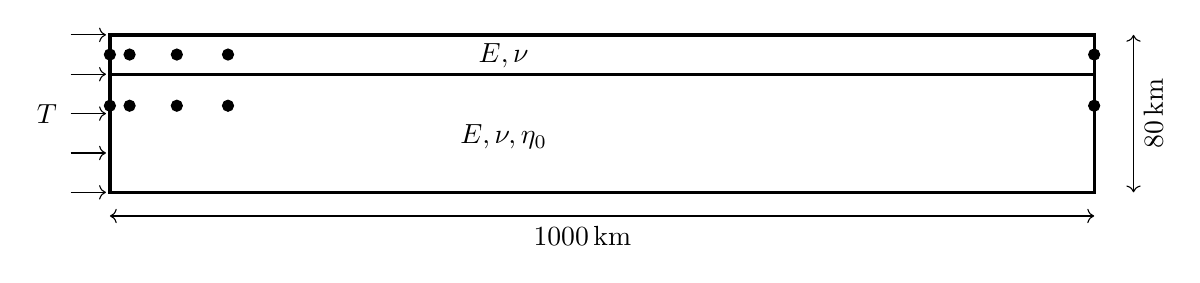
\begin{tikzpicture}
%\draw[step=0.5cm,gray,very thin] (0,0) grid (15,4); %background grid
\draw[very thick] (1,1)--(13.5,1)--(13.5,3)--(1,3)--cycle;  
\draw[very thick] (1,2.5)--(13.5,2.5);  
\draw[<->] (1,0.7)--(13.5,0.7);
\draw[<->] (14,1)--(14,3);
\node[] at (7,0.45) {$\SI{1000}{\km}$};
\node[rotate=90] at (14.25,2) {$\SI{80}{\km}$};
\node[] at (6,2.73) {$E,\nu$};
\node[] at (6,1.7) {$E,\nu,\eta_0$};
\draw[->] (0.5,3)--(0.95,3);
\draw[->] (0.5,2.5)--(0.95,2.5);
\draw[->] (0.5,2)--(0.95,2);
\draw[->] (0.5,1.5)--(0.95,1.5);
\draw[->] (0.5,1)--(0.95,1);
\node[] at (0.2,2) {$T$};

\filldraw[black] (1,2.75) circle (2pt);
\filldraw[black] (1,2.1) circle (2pt);

\filldraw[black] (1.25,2.75) circle (2pt);
\filldraw[black] (1.25,2.1) circle (2pt);

\filldraw[black] (1.85,2.75) circle (2pt);
\filldraw[black] (1.85,2.1) circle (2pt);

\filldraw[black] (2.5,2.75) circle (2pt);
\filldraw[black] (2.5,2.1) circle (2pt);

\filldraw[black] (13.5,2.75) circle (2pt);
\filldraw[black] (13.5,2.1) circle (2pt);
\end{tikzpicture}
\end{center}


After a thorough read of the paper, I have noticed quite a few problems:
\begin{itemize}
\item the paper is old and has been digitized but the figures are missing a lot of lines/shades/points ... this could be remedied by finding the article in a library.
\item in the intro it is stated: "Here we investigate the response of a lithosphere divided into upper elastic and lower uniform visco-elastic layers to simple boundary force and body force systems." The authors later talk about 'isostatic forces' opposing flexure. This means that buoyancy forces should be taken into account but there is no information about densities or gravity values!
\item little uncertainty about boundary conditions. is it free slip or no-slip on the right side ? Looking at fig 4, it looks like the vertical displacement is zero at x=1000km?
\item a Maxwell elasto-viscous rheology is used but this is only mentioned in the Appendix
\item the dimensions of the thinned or thickened areas is simply not mentioned. 
\item Fig~1 shows triangular elements. No mention is made of resolution, type of element, ndofs, resolution tests, any numerical detail whatsoever. Given the age of the paper, I would guess $P_1$
elements.
\item In the appendix they equate the viscous strain rate to $\sigma/4\eta$. Why 4 ?
\item it is also not clear whether the domain is ALE or fully Lagrangian: does it shorten?
\item the value of $T$ is never specified!
\item the paper was published 45 years ago, it is extremely unlikely any of the two authors is still available 
\end{itemize}

\begin{center}
\fbox{\includegraphics[width=16cm]{images/viscoelasticity/kubo77}}\\
{\captionfont Taken from \textcite{kubo77}. Measurement locations are indicated on 
the setup figure above. probably should be reversed}
\end{center}






%..........................................................
\subsection{Parallel-Plate Viscometer Problem - SNAC manual \label{v-e-snac}}

A parallel-plate viscometer problem is simulated, in which viscoelastic material is squeezed between two
parallel plates. The plates are moving at a constant velocity, $v_0$. Each plate has the length of $2L$ and 
is at a distance $2h$ from the other. No slip is assumed between the material and the plates. The approximate
analytical solution is given in the book by \textcite{jaeg69} (1969).

Model Setup: $L = 10~\si{\meter}$, $h=5~\si{\meter}$, viscosity $\eta=10^9~\si{\pascal\second}$, 
bulk modulus $K= 1.5~\si{\giga\pascal}$, shear modulus $\mu = 500~\si{\mega\pascal}$,
$v_0 = 10^{-4}~\si{\meter\per\second}$, $dt = 1~\si{\second}$ (results compared after 500 time steps),
mesh size: $20\times 10~\si{\meter}$, each element is a $1~\si{\meter}$ cube.

Due to the assumption of the original problem setup, artificial forces should be added to left and right
surfaces.

\begin{center}
\includegraphics[width=8cm]{images/viscoelasticity/snac_5}
\includegraphics[width=8cm]{images/viscoelasticity/snac_6}\\
{\captionfont 
Left: The initial mesh (blue) with the velocity boundary condition (red arrows);
Right: The second invariant of stress and velocities plotted on the deformed mesh. Colored arrows are
for SNAC’s solution, black ones for the analytic solution.}
\end{center}

$K=\lambda + \frac23 \mu$ so $\lambda=\frac{3500}{3}MPa$ ?

From wikipedia\footnote{\url{https://en.wikipedia.org/wiki/Lame_parameters}}
\[
\nu = \frac{3K-2\mu}{2(3K+\mu)} 
= \frac{4500-2*500}{2(4500+500)}
= \frac{3500}{10000}
= 0.35
\]
so we find that the material is {\color{orange} compressible $\nu=0.35$}

\[
E=\frac{9K\mu}{3K+\mu} 
=\frac{9*1500*500 MPa^2}{4500+500 MPa}
=\frac{9*1500*500}{5000} MPa
= 1350Mpa
\]


%..........................................................
\subsection{Relaxation after extention - Hassani syllabus}


{\color{orange} compressible $\nu=0.25$}

Un essai de relaxation consiste à imposer à un instant donné une déformation que 
l’on maintient constante par la suite. On observe alors comment évolue la contrainte au cours du temps.

The setup of the experiment is shown in the following figure:

\begin{center}
\includegraphics[width=9cm]{images/viscoelasticity/hassani_1}
\end{center}

The total duration of the experiment is $T=\SI{5}{\year}\simeq \SI{15.75e7}{\second}$.
The duration of the loading is $T/10=\SI{6}{months}$ while the duration 
of the subsequent relaxation is then $9T/10\simeq 4.5~\si{\year}$.

The loading velocity is $v=\SI{1}{\mm\per\year}\simeq \SI{3.17e-11}{\meter\per\second}$.
The sample has size $L\times L/2 = 20\times10\si{cm}$ and 
the strain rate is then $v/L \simeq \SI{1.5e-10}{\per\second}$.
Young's modulus is set to \SI{1e11}{\pascal} and the Poisson ratio is 0.25, i.e.
$\mu=40~\si{GPa}$. The viscosity is set to $\eta_0=\SI{1e18}{\pascal\second}$.
The Maxwell time is then $t_M=\eta/\mu=0.8~\si{\year}$, which is also the time it takes 
to reduce the maximum stress by a factor $e$.

\begin{center}
\includegraphics[width=6cm]{images/viscoelasticity/hassani_2}
\end{center}







%-------------------------------------------------------------------------
\subsection{Role of elasticity in slab bending - \textcite{fogm14} (2014)}

\begin{center}
\includegraphics[width=8cm]{images/viscoelasticity/fogm14b}
\includegraphics[width=8.5cm]{images/viscoelasticity/fogm14c}\\
\end{center}












%-------------------------------------------------------------------------
\subsection{Shear test in 2D - \textcite{famc14} (2014)}

This experiment consists of a viscoelastic material undergoing simple shear at a constant 
rate from a time $t_0$ though to $t_{max}$. At $t_{max}$, the shearing velocity is taken 
to zero using a no-slip velocity boundary condition. The viscoelastic stresses then decay
with time while the material deformation rate remains zero. The $xy$ component of stored 
stress, i.e. the nonviscous portion of the total stress, is given by
\begin{align}
\tau_{xy}^{stor} 
&= 
\exp -\frac{\mu}{\eta}t 
\left(
C_2 \cos\left( \frac{Vt}{h}\right)
-C_1 \sin\left( \frac{Vt}{h}\right)
\right)
-C_2 & \textrm{if} \; t<t_{max} \nn\\
&= \left[\exp -\frac{\mu}{\eta}t_{max} 
\left(
C_2 \cos\left( \frac{Vt}{h}\right)
-C_1 \sin\left( \frac{Vt}{h}\right)
\right)
-C_2 \right] \exp -\frac{\mu}{\eta}(t-t_{max})
& \textrm{if} \; t>t_{max} 
\end{align}
where $V$ is the shear velocity along the top wall boundary, 
$h$ is the height of the box,
\[
C_1=-\frac{V^2 \eta^2 \mu}{\mu^2 h^2 + V^2 \eta^2}
\]
\[
C_2=-\frac{Vh\eta \mu^2}{\mu^2 h^2 + V^2 \eta^2}
\]



\begin{center}
\includegraphics[width=8cm]{images/viscoelasticity/famc14a}\\
\captionfont{The xy component of dimensionless stored stress with dimensionless time 
for the 2-D viscoelastic material undergoing simple shear and relaxation. Nondimensional 
material parameters of $\eta=10^2$, $\mu=10^2$, $t_M=1$, $V=0.05$, $h=1$ 
with $\Delta t_e\in[0.01,1]$ and $\Delta t_c=\frac13 \Delta t_e$.
}
\end{center}

Figure above shows the resulting xy component of the deviatoric stored stress term for a 2-D viscoelastic material across a range of $\Delta t_e$. 
At longer $\Delta t_e$, the stored stress appears under resolved, indicating these larger elastic time step values capture dynamics that occur on time scales approximately equal to or greater than the Maxwell relaxation time, that is with a portion of viscous deformation. For shorter $\Delta t_e$,
the numerically calculated stress approaches the analytic solution, indicating that the elastic time step is
sufficiently small to fully capture the elastic stored stresses produced within the material under the
applied strain rate.







%-------------------------------------------------------------------------
\subsection{Tortion test in 3D - \textcite{famc14} (2014)}

insert here eq 9 of paper

The analytic solution outlined by equation (9) can be extended from this 
essentially 1-D test into 3-D by applying the shear velocity in the x-z plane. 
Testing of the full viscoelastic implementation including the
rotation terms is possible by placing this 3-D shear test in a 
coordinate system under going solid body rotation. 

\begin{center}
\includegraphics[width=8cm]{images/viscoelasticity/famc14b}\\
\captionfont{
The $xy$ and $yz$ stress components of a material undergoing simple shear within 
a 3D rotating reference frame. Nondimensional material parameters of 
$\eta=100$, $\mu=100$, $\alpha=1$, $V=0.3$, $h=1$, $t_{max}=0.5$
and $\omega=42$. Note the coordinate system for this test has the $y$ axis in the vertical 
with the $z$ axis in plane. Results for a first (crosses) and 
fourth- (lines) order accurate Jaumann stress rate integration scheme are shown 
in comparison to the analytical solution (black) given by equation (9) within the rotating frame.
}
\end{center}

Figure above shows the evolution of the stress in comparison to the analytical solution of equation (9)
placed within the rotating frame. The rotating frame is achieved by imposing a velocity boundary condition
of a constant solid body rotation about the y axis in addition to the shearing rate. The stress within this
rotating frame is given by equation (9), with the stress in the nonrotating frame found by 
applying a rotation matrix, $R$, to the nonrotating stress solution. 
That is, $\tau=R^{-1}\tau'R$, where $'$ denotes the rotated frame, $R$ is
the rotation matrix about the y axis given by 
\[
R= \left(
\begin{array}{ccc}
\cos\theta &0 & \sin\theta \\
0 & 1 & 0 \\
-\sin\theta & 0 & \cos\theta
\end{array}
\right)
\]
with $\theta=\omega t$, $\omega$ being the dimensionless rotation rate. 
The stress components shown in Figure 1b from within the 
nonrotating frame can then be given by $\tau^{stor}_{xy}=\tau^{stor'}_{xy} \cos\theta$
and $\tau^{stor}_{yz}=\tau^{stor'}_{yz} \sin\theta$.
It can be seen that, using a higher-order Jaumann stress rate advection scheme 
results in accurate stress advection and rotation within the full
3-D space plus time domain. It should be noted here that the velocity field used in 
this test was chosen to rigorously test the rotational terms in equation (6). 
Whether these rotational terms are required for individual models is dependent upon 
the model setup. For subducting slabs at a constant curvature, the individual 
parcels of material experience purely rotational effects, accounting for this within the stress history term
would then be required for consistency.

{\color{red} finish!}










%-------------------------------------------------------------------------
\subsection{Cylindrical tunnel - Segall book (?)}

{\color{orange} compressible $\nu=0.25$}

communicated to me by L .van de Wiel.

This is a cylindrical tunnel (2D magma chamber) in an infinite space, with certain radius.
The material close around the hole is warm, and and such viscous. The material further from the hole is cold, and purely elastic. (accomplished by setting and absurdly high viscosity) 
There is a clear transition radius between the two properties
The hole contains a pressure, causing the space to expand.

After the initial elastic deformation, viscous deformation continues in the viscous region of the domain.
I have the implementation of the analytical solution attached to save you time.

See plot with radial deformation for t=0 (green), t=300s (red), t=600s (blue), and t=3000s (black).
thin line is analytic, points are numeric.
(with parameters and size parameters as in analytic.f)


\begin{center}
\includegraphics[width=8cm]{images/viscoelasticity/radialDisp}
\end{center}










%..........................................................
\subsection{Relevant literature \& various notes}



\begin{itemize}
\item convection of viscoelastic fluids: 
\textcite{hard91}, \textcite{momy93}, 
\textcite{zhgm96}, \textcite{modm02}, 
\textcite{mure05}, \textcite{likh05a},  
\textcite{likh05b}, \textcite{fukk08}


\item stress buildup associated with viscoelastic rheology 
\textcite{kubo77}, \textcite{kupa84}, \textcite{pocp93}, \textcite{mapo09}

\item viscoelastic effects on geodynamical pbs involving gravitational instability 
\textcite{pocp93,kabe07,bumo08,scbe08}, 
\textcite{hamy95} 

\item large strain  eulerian viscoelasticity 
\textcite{scps01,vapy01,coll06,moql07,fukk08,poso08}

\end{itemize}

\textcite{famc14} states 
``Funiciello et al. [2003] implemented a viscoelastic rheology in numerical models of subduction, performing a
range of numerical simulations to investigate its effect on subducting slab dynamics. Similar methodologies have addressed the details of viscoelastic stress within the bending zone during subduction, although a comparison between viscous and viscoelastic rheology was lacking [Capitanio et al., 2009; Capitanio and Morra, 2012].
Muhlhaus and Regenauer-Lieb [2005] and Moresi et al. [2002] have studied the role of elasticity in mantle convection, comparing the viscous case to that of viscoelastic, and Kaus and Becker [2007] discussed the effect of elasticity on layered Rayleigh-Taylor instabilities. However, a systematic study into the effects of elastic stresses on models of free subduction has yet to be completed. Morra and Regenauer-Lieb [2006], Funiciello et al. [2003], Capitanio et al. [2007], Yamato et al. [2007], and Royden and Husson [2006] have included a viscoelastic slab in subduction models, without explicitly studying the effects of the elastic component across a range of parameters.''


Check early paper by Braun \& Beaumont (1987) \cite{brbe87}

\textcite{asmo12} (2012)
\textcite{hepk14} (2014)
\textcite{daws16} (2016)
\textcite{thkp15} (2015)
\textcite{beps10} (2010)
\textcite{samb20} (2020)
\textcite{vosc15} (2015)
\textcite{nalr12} (2012)
\textcite{pelt74} (1974)
\textcite{kaps04} (2004)
 \label{chapt:viscoelasticity} %%%%%%%%%%%%%%%%%%%%%%%%%%%%%%%%%%%

%%%%%%%%%%%%%%%%%%%%%%%%%%%%%%%%%%%%%%%%%%%%%%%%%%%%%%%%%%%%%%%%%%%%%%%%%%%%%%%%%%%%%%%%%%%%%%%%%%%
%\chapter{Geophysical data} %%%%%%%%%%%%%%%%%%%%%%%%%%%%%%%%%%%%%%%%%%%%%%%%%%%%%%%%%%%%%%%%%%%%%%%
\chapter{Geophysical data} 

\newpage %-----------------------------------------------------------------------------------------
\section{Earth: The PREM model} \label{ss:prem} 
Let us define $x=r/R$.
Following table I of Dziewonski \& Anderson (1981) \cite{dzan81} \index{general}{P.R.E.M.}
we have 

\begin{itemize}
\item for the inner core $0<r<1221.5\si{\km}$:
\[
\rho(x) =13.0885-8.8381 x^2
\]
\item for the outer core $1221.5<r<3480$km:
\[
\rho(x)=12.5815-1.2638x-3.6426x^2-5.5281x^3
\]
\item for the Lower mantle $3480<r<5701$km:
\[
\rho(x)=7.9565-6.4761x+5.5283x^2-3.0807x^3
\]
\item for the transition zone 1 $5701<r<5771$km:
\[
\rho(x)=5.3197-1.4836x
\]
\item for the transition zone 2 $5771<r<5971$km:
\[
\rho(x)=11.2494-8.0298x
\]
\item for the transition zone 3 $5971<r<6151$km:
\[
\rho(x)=7.1089-3.8045x
\]
\item Low velocity zone $6151<r<6291$km:
\[
\rho(x)=2.6910+0.6924x
\]
\item LID  $6291<r<6346.6$km:
\[
\rho(x)=2.6910+0.6924x
\]
\item Lower Crust $6346.6<r<6356$km:
\[
\rho(x)=2.9
\]
\item Upper Crust $6356<r<6368$km:
\[
\rho(x)=2.6
\]
\item Ocean $6368<r<6371$km
\[
\rho(x)=1.020
\]
\end{itemize}

\noindent Note that the returned densities should be multiplied by 1000 to obtain 
units of kg/m$^3$.

One can verify that the functions above yield the familiar PREM density profile:
\begin{center}
\includegraphics[width=6cm]{images/prem/rho.pdf}
\end{center}

Following Eq.~(\ref{eqn_g_rad_comp}), the radial component of the gravitational 
acceleration at a position $r$ outside of the Earth is given by:

\begin{equation}
g_r(r) 
= - \frac{1}{r^2} \int_0^r 4\pi {\cal G} \rho(r') r'^2 dr'
= - \frac{4 \pi {\cal G}}{r^2} \int_0^r \rho(r') r'^2 dr'
\end{equation}
 
This integral can be broken up into layer integrals and we can compute the contribution 
of each layer to the gravity value $g_r(r)$.

Let us remember that $x=r/R$ so $dr = R dx$. 
\begin{eqnarray}
g_{ic}(r)
&=&  \frac{4 \pi {\cal G}}{r^2} \int_0^{1221.5} (13.0885-8.8381 (r/R)^2) r^2 dr \nn\\
&=&  \frac{4 \pi {\cal G} R^3}{r^2}  \int_0^{1221.5/6371} (13.0885-8.8381 x^2) x^2 dx \nn\\
&\simeq& 0.0302907  \frac{4 \pi {\cal G} R^3}{r^2}\nn\\
g_{oc}(r)
&=&  \frac{4 \pi {\cal G} R^3}{r^2} 
\int_{1221.5/6371}^{3480/6371} (12.5815-1.2638x-3.6426x^2-5.5281x^3)x^2 dx 
\simeq 0.56663  \frac{4 \pi {\cal G} R^3}{r^2}\nn\\
g_{lm}(r) 
&=& \int_{3480/6371}^{5701/6371} (7.9565-6.4761x+5.5283x^2-3.0807x^3)x^2 dx 
\simeq 0.904793 \frac{4 \pi {\cal G} R^3}{r^2}\nn\\
g_{tz1}(r) 
&=& \int_{5701/6371}^{5771/6371} (5.3197-1.4836x)x^2 dx 
\simeq 0.0354823 \frac{4 \pi {\cal G} R^3}{r^2}\nn\\
g_{tz2}(r)
&=& \int_{5771/6371}^{5971/6371}   (11.2494-8.0298x)x^2 dx \simeq  0.1026 \frac{4 \pi {\cal G} R^3}{r^2}\nn\\
g_{tz3}(r)
&=& \int_{5971/6371}^{6151/6371}   (7.1089-3.8045x)x^2 dx  \simeq 0.0892215 \frac{4 \pi {\cal G} R^3}{r^2}\nn\\
g_{lvz} 
&=&  \int_{6151/6371}^{6291/6371} (2.6910+0.6924x) x^2 dx  \simeq  0.0705516 \frac{4 \pi {\cal G} R^3}{r^2}\nn\\
g_{lid}
&=& \int_{6291/6371}^{6346.6/6371} (2.6910+0.6924x)x^2 dx \simeq 0.0289968 \frac{4 \pi {\cal G} R^3}{r^2}\nn\\
g_{lc}
&=& \int_{6346.6/6371}^{6356/6371} 2.9 x^2 dx  \simeq 0.00425234 \frac{4 \pi {\cal G} R^3}{r^2}\nn\\
g_{uc}
&=& \int_{6356/6371}^{6368/6371} 2.6 x^2 dx  \simeq 0.00488337 \frac{4 \pi {\cal G} R^3}{r^2}\nn\\
g_{o}
&=& \int_{6368/6371}^{1} 1.020 x^2 dx  \simeq 0.000480075 \frac{4 \pi {\cal G} R^3}{r^2}
\end{eqnarray}


Finally 
\begin{eqnarray}
|g_r(r)| 
&=&  g_{ic}(r) + g_{oc}(r) + g_{lm}(r) + g_{tz1}(r) + g_{tz2}(r) + g_{tz3}(r) + 
g_{lvz}(r) + g_{lid}(r) + g_{lc}(r) + g_{uc}(r) + g_{o}(r) \nn\\
&=& 
\frac{4 \pi {\cal G} R^3}{r^2}
(
0.0302907 + 
0.56663 +
0.904793 +
0.0354823 +
0.1026 +
0.0892215+ \nn\\
&& 
0.0705516 +
0.0289968 +
0.00425234+
0.00488337+
0.000480075
  ) \nn\\
&\simeq& 
\frac{4 \pi {\cal G} R^3}{r^2} \nn
1.838181685
\end{eqnarray}

At the surface of the Earth, $r=R$ so we arrive at (after multiplying by 1000, see comment above): 
\[
\boxed{
g_{\tiny PREM}(R) \simeq 
4 \pi \cdot 6.67408\times 10^{-11}\cdot  6371\times 10^3 \cdot 1.838181685
\simeq 9.82194
}
\]

All these calculations should be rechecked, although obviously the obtained value makes much sense. 

 %-------------------------------------
\newpage %-----------------------------------------------------------------------------------------
\section{Earth: From 1D tomography to density/temperature} 
The mantle is heterogeneous but it is also inaccessible. This means that one must rely on indirect methods 
to probe its structure. Seismic tomography is a technique for imaging the subsurface of 
the Earth with seismic waves produced by earthquakes or explosions. 
P-, S-, and surface waves can be used for tomographic models of different resolutions.

Seismic velocity is a meaningful parameter for the interior dynamics of the
Earth because there exists a direct relation between seismic velocity and density. 
Such a relation was analysed experimentally by (for instance) Barton (1986) who 
used laboratory measurements of P-wave seismic velocity and density of rocks \cite{bart86}. 

Fourty years later or so, a crucial question remains: what is the exact form of the 
relation between density and seismic velocity for the entire Earth’s mantle?

I will here not go into the details of the underlying theories and their approximations but 
will show a few useful results. 

From tomography to density, the workflow is usually as follows:
\[
d \ln V_p \rightarrow d \ln V_s \rightarrow d \ln \rho \rightarrow d\rho
\]
Note that if the method is based on shear wave tomography the conversion $d \ln V_p \rightarrow d \ln V_s$
is not necessary. 
Also the last step $d \ln \rho \rightarrow d\rho$ requires a background density field, 
often taken to be either the PREM model of AK135 (see Section~\ref{ss:prem}). 

On the following plots are shown radial averages of the ratio $d \ln V_s/d\ln V_p$ and 
$d\ln \rho/d \ln V_s$:

\begin{center}
\includegraphics[height=5cm]{images/dlnvsdlnrho/moek16b}
\includegraphics[height=5cm]{images/dlnvsdlnrho/moek16a}\\
{\captionfont Taken from Moulik \& Ekstrom (2016) \cite{moek16}}
\end{center}

\begin{center}
\includegraphics[height=6cm]{images/dlnvsdlnrho/xi.pdf}\\
{\captionfont Profiles of scaling factor $\xi=d \ln \rho/d\ln V_s$. Data from 
Steinberger \& Calderwood (2006) \cite{stca06} and Moulik \& Ekstrom (2016) \cite{moek16}.
Data available in images/dlnrhodlnvs/} 
\end{center}



\Literature: \cite{roma01}
 %---------------------
\newpage %-----------------------------------------------------------------------------------------
\section{Earth: radial viscosity profile \label{ss:viscprof}} 

\begin{center}
\includegraphics[width=5cm]{images/viscosity_profile/yohk01}\\
{\captionfont Radial viscosity profile of the reference model. 3-layered model is adopted: 
the lithosphere (0 km to 150 km), the upper mantle (150 km to 670km) 
and the lower mantle (670 km to 2900 km). Taken from \cite{yohk01}}
\end{center}

\begin{center}
\includegraphics[width=5cm]{images/viscosity_profile/stca06}\\
{\captionfont Taken from \cite{stca06}}
\end{center}



 %----------
\newpage %-----------------------------------------------------------------------------------------
\section{Earth: radial temperature profile \label{ss:adiab}} 

[from ASPECT manual]



---------------------------------------------
\paragraph{Isentropic gradient}

The material properties also define the slope of the adiabat (the change in temperature with
pressure at constant entropy) at all pressures and temperatures. Using the cyclic relation,
we can define this slope in terms of partial differentials of the entropy with respect to pressure
and temperature:
\begin{eqnarray}
\left( \frac{\partial T}{\partial p} \right)_{S} 
&=& - \left( \frac{\partial T}{\partial S} \right)_{p} \left( \frac{\partial S}{\partial p} \right)_{T} \\
&=& - \left( \frac{T}{C_p} \right) \left( - \frac{\alpha}{\rho} \right) \\
&=& \frac{\alpha T}{\rho C_p} \label{eq:mm_isentropic_gradient}
\end{eqnarray}
This expression does not pose a constraint on the material properties, but in order to be 
self-consistent, the adiabat must be computed following this relation.

For complex material models, obtaining analytical functions which obey all these relations
may be a non-trivial exercise. Furthermore, it is often not immediately clear when a
given formulation is thermodynamically inconsistent. Indeed, both the
thermodynamic and the geodynamic literature contain many equations of
state and material parameterizations which do not obey these 
relations! This may not invalidate the results obtained with these 
models, but it is a point worth keeping in mind as the geodynamics
community moves to more complicated and more realistic parameterizations.

\emph{A final note of warning: Some compressible formulations in \aspect{}
  (Section~\ref{sec:mass-conservation-approximation}) use the isothermal compressibility,
  while others use the isentropic compressibility. Fully self-consistent material models must
  either specify what approximation of the compressible equations they are consistent with
  (see Section~\ref{sec:approximate-equations}), or have a switch so that they use the correct
  compressibility for each of the different approximations. The conversion between isothermal
  and isentropic compressibilities is given in~\eqref{eq:mm_isentropic_compressibility}.}

--------------------------------------------------

\paragraph{Initial conditions and the adiabatic pressure/temperature}

The thermo-mechanically coupled (Navier-)Stokes 
equations require us to
pose initial conditions for the temperature
Note that the equations
themselves do not require that initial conditions are specified for
the velocity and pressure variables (since there are no time
derivatives on these variables in the model).

Nevertheless, a nonlinear solver will have difficulty converging to
the correct solution if we start with a completely unphysical pressure
for models in which coefficients such as density $\rho$ and viscosity
$\eta$ depend on the pressure and temperature. To this end, \aspect{}
uses pressure and temperature fields $p_{\textrm{ad}}(z),
T_{\textrm{ad}}(z)$ computed in the adiabatic conditions model
(see Section~\ref{parameters:Adiabatic_20conditions_20model}).
By default, these fields satisfy adiabatic conditions:
\begin{align}
\rho C_p \frac{\textrm{d}}{\textrm{d}z} T_{\textrm{ad}}(z)
&=
\frac{\partial\rho}{\partial T} T_{\textrm{ad}}(z) g_z,
\\
\frac{\textrm{d}}{\textrm{d}z} p_{\textrm{ad}}(z)
&=
\rho g_z,
\end{align}
where strictly speaking $g_z$ is the magnitude of the vertical
component of the gravity vector field, but in practice we take the
magnitude of the entire gravity vector.

These equations can be integrated numerically starting at $z=0$, using
the depth dependent gravity field and values of the coefficients
$\rho=\rho(p,T,z), C_p=C_p(p,T,z)$. As starting conditions at $z=0$ we
choose a pressure $p_{\textrm{ad}}(0)$ equal to the average surface
pressure (often chosen to be zero, see Section~\ref{sec:pressure}),
and an adiabatic surface temperature $T_{\textrm{ad}}(0)$ that is
also selected in the input parameter file.
%\index[prmindex]{Adiabatic surface temperature}
%\index[prmindexfull]{Adiabatic surface temperature}

\note{The adiabatic surface temperature is often chosen significantly
  higher than the actual surface temperature. For example, on earth,
  the actual surface temperature is on the order of 290 K, whereas a
  reasonable adiabatic surface temperature is maybe 1600 K. The reason
  is that the bulk of the mantle is more or less in thermal equilibrium
  with a thermal profile that corresponds to the latter temperature,
  whereas the very low actual surface temperature and the very high
  bottom temperature at the core-mantle boundary simply induce a
  thermal boundary layer. Since the temperature and pressure profile
  we compute using the equations above are simply meant to be good
  starting points for nonlinear solvers, it is important to choose
  this profile in such a way that it covers most of the mantle well;
  choosing an adiabatic surface temperature of 290 K would yield a
  temperature and pressure profile that is wrong almost throughout the
  entire mantle.}

For instance, let us consider $\alpha=3\cdot 10^{-5}$, 
$g_z=10$, $C_p=1250$, $\rho=\rho_0(1-\alpha (T-T_0)$ so that 
$\frac{\partial\rho}{\partial T} = -\alpha \rho_0$ 
with $\rho_0=3300$.

Then we must solve the following equation
\[
\rho_0(1-\alpha(T-T_0)) C_p \frac{\textrm{d}T}{\textrm{d}z} 
=
- \alpha T^2  g_z
\]

----------------------------------

In Verhoogen (1951) \cite{verh51}:
As is well known, the adiabatic gradient may be written as
\[
\frac{dT}{dP} = \alpha T /\rho C_p
\]
If hydrostatic equilibrium is assumed, the pressure varies with depth $h$ as 
$dP = \rho g dh$, so that
\[
\frac{d \ln T}{dh} = \frac{\alpha g}{C_p}
\]
from which the temperature $T$ at any depth $h$ may be computed as a function of the temperature
at any assigned depth if the ratio $\alpha/C_p$ 
is known at all depths ($g$, the acceleration of gravity, will
be taken as constant in the mantle).

----------------------------------
\begin{center}
\includegraphics[width=12cm]{images/adiabatic/drawing.png}
{\captionfont Adiabatic temperature profiles.}
\end{center}

----------------------------------


\begin{center}
\includegraphics[width=7cm]{images/adiabatic/kayy10a}
\includegraphics[width=7cm]{images/adiabatic/kayy10b}\\
{\captionfont Taken from Katsura et al (2010) \cite{kayy10}.
Left: The adiabatic temperature distributions in the mantle. The three solid lines
denote the temperature distributions proposed in this study using three different
pressure scales. Those proposed by the previous studies are shown for comparison
(BS81: Brown and Shankland, 1981; IK89: Ito and Katsura, 1989; dS00: da Silva et al.,
2000; SD08: Stacey and Davis, 2008). The mantle solidus proposed by Hirschmann
(2000) is also shown.
Right:
Adiabatic temperature gradient in the mantle. The adiabatic temperature gradient 
abruptly increases in association with the olivine–wadsleyite,
wadsleyite–ringwoodite, ringwoodite–perovskite + periclase transitions, as is the
case for the thermal expansion. The adiabatic temperature gradients given in the
previous studies are also shown for comparison (BS81: Brown and Shankland, 1981;
SD08: Stacey and Davis, 2008).
}
\end{center}

----------------------------------

From DyMaLi: In the interior of a convecting medium temperatures follow an adiabatic profile. 
At the top and bottom of a convecting layer thermal boundary layers with large thermal gradients form. 
The interior is thermally well mixed and therefore essentially isothermal, with a slight increase 
of temperatures with depth due to the effect of pressure.
For example in the Earth’s mantle the geothermal gradient ∂T /∂z is about 20C/km near the 
surface and about 0.3C/km in the interior of the mantle. This small gradient in the 
interior is the adiabatic gradient. If a small
volume of material is moved to shallower depth is experiences a slight increase in volume 
due to the decreasing pressure and associated with this a slight decrease in temperature. 
This change in temperature is the adiabatic temperature change.

The adiabatic gradient can be determined from the thermodynamics relation between entropy per unit mass S,
temperature T, and pressure P:
\[
dS = \left( \frac{dS}{dT}\right)_P dT +  \left( \frac{dS}{dP}\right)_T dP
=
\frac{C_p }{T} dT - \frac{\alpha}{\rho} dP
\]
In case of a reversible adiabatic process the entropy change is zero, and so the adiabatic gradient is:
\[
\left( \frac{dT}{dP}\right)_S = \frac{\alpha T}{\rho C_p} 
\]
The gradient can also be expressed in terms of depth, remembering that $d p = \rho gdz$ 
in a hydrostatic fluid:
\[
\left( \frac{dT}{dz}\right)_S = \frac{\alpha g T}{C_p} 
\]
Thus to determine the adiabatic gradient one needs values of $\alpha$ 
and $C_p$ with depth. These are obtained from laboratory experiments.

One also needs an estimate of density as a function of depth, which is generally determined
from seismology. 
Integration of the adiabatic gradient in terms of pressure then gives
temperature as a function of pressure. 
Temperature as a function of depth is obtained by integrating the density
distribution to obtain g as a function of depth.

not finished
----------------------------------

Vol07\_02


This adiabaticity hypothesis should, however, not
be taken too literally (Jeanloz and Morris, 1987 \cite{jemo87}). In
most numerical simulations, the resulting averaged
geotherm can be far (a few hundred kelvins) from
adiabatic (Bunge et al., 2001 \cite{burm01}). First, radioactive heat-
ing, dissipation, and diffusion are never totally
negligible, second, even if each fluid parcel follows
its own adiabatic geotherm, the average geotherm
may not correspond to any particular adiabat.




----------------------------------

\Literature: 
{\it On the thermal gradient in the Earth’s deep interior}, Tirone (2016) \cite{tiro16} \\
{\it Is the mantle geotherm subadiabatic}, Jeanloz \& Morris (1987) \cite{jemo87} \\

Bunge (2005) \cite{bung05}

Dannberg \& Solomatov \cite{daso15} + supplementary!

 %-------------------
\newpage %-----------------------------------------------------------------------------------------
\section{Earth: radial thermal expansion profile} \begin{flushright} {\tiny {\color{gray} thermal\_expansion\_profile.tex}} \end{flushright}


\begin{center}
\includegraphics[width=7cm]{images/thermal_expansion/pape95}\\
{\captionfont 
Taken from \textcite{pape95} (1995).}
\end{center}

\begin{center}
\includegraphics[width=10cm]{images/thermal_expansion/buja04}\\
{\captionfont 
Taken from \textcite{buja04} (2004). To dimensionalize, multiply 
the thermal expansivity (thick solid line) 
by $\alpha_0=2\cdot 10^{-5}~\si{\per\kelvin}$.
}
\end{center}


\begin{center}
\includegraphics[width=10cm]{images/thermal_expansion/stca06.jpg}\\
{\captionfont Taken from \textcite{stca06}.}
\end{center}

see Matyska \etal (2011) \cite{mayw11}

Mantle convection with internal heating and pressure-dependent thermal expansivity, Leitch \etal (1991) \cite{leys91}

Eq(8) of Hassan \etal \cite{hafg15}

\begin{center}
\includegraphics[width=10cm]{images/thermal_expansion/nemi23}\\
{\captionfont Taken from \textcite{nemi23}.}
\end{center}
 %--------------
\newpage %-----------------------------------------------------------------------------------------
\section{Earth: radial density profile} \begin{flushright} {\tiny {\color{gray} density\_profile.tex}} \end{flushright}
%~~~~~~~~~~~~~~~~~~~~~~~~~~~~~~~~~~~~~~~~~~~~~~~~~~~~~~~~~~~~~~~~~~~~~~~~~~~~~~~~~~~~~~~~~~~~~~~~~~

\begin{center}
\includegraphics[width=12cm]{images/density_profile/density_profile}
\end{center}

\Literature: Kennett (1998) \cite{kenn98}

\textcolor[RGB]{220,220,220}{\rule{\linewidth}{0.2pt}}

\begin{center}
\includegraphics[width=8cm]{images/density_profile/chmo95}\\
{\captionfont Taken from \textcite{chmo95} (1995).
A model for average crustal petrology versus depth consistent with average velocity depth
profile (solid circles) and velocity depth curves for common rock types (open symbols). 
Variations of density and SiO 2 content with depth are from rock percentages
shown on the left.} 
\end{center}


\textcolor[RGB]{220,220,220}{\rule{\linewidth}{0.2pt}}

Let us look at the density and pressure profiles in a 1D isothermal 'planet'. 
We start from 
\[
-\vec\nabla p + \rho \vec{g} = \vec{0}
\]
In 1D, and assuming $\vec{g}=-g \vec{e}_z$:
\[
-\frac{dp}{dz}-\rho g=0
\]
or
\[
\frac{dp}{dz}= -\rho g
\]
Assuming $\rho$ and $g$ constant in the domain $z\in [0,L]$, we can solve this ODE and we obtain:
\[
p(z) = \rho g (L-z)
\]
Let us now turn to the case of an isothermal but compressible fluid. 
Its density is now given by 
\[
\rho(p) = \rho_0(1-\beta p)
\]
where $\beta$ is the compressibility (assumed to be constant in the domain). We must then solve
\begin{eqnarray}
\frac{dp}{dz}= -\rho_0(1-\beta p) g
&\Rightarrow&
\frac{dp}{1-\beta p} = -\rho_0 g dz \nonumber\\
&\Rightarrow&
\int \frac{dp}{1-\beta p} = -\int \rho_0 g dz \nonumber\\
&\Rightarrow&
-\frac{1}{\beta} \ln (1-\beta p) = -\rho_0 g z + C \nonumber\\
&\Rightarrow&
\ln (1-\beta p) = \beta \rho_0 g z + D \nonumber\\
&\Rightarrow&
1 -\beta p = \exp \left( \beta \rho_0 g z + D  \right) \nonumber\\
&\Rightarrow&
p(z) = \frac{1}{\beta} \left[ 1- \exp \left( \beta \rho_0 g z + D  \right) \right] \nonumber\\
\end{eqnarray}
At $z=L$ we require $p=0$ so we obtain
\[
p(z) = \frac{1}{\beta} \left[ 1- \exp \left( \beta \rho_0 g (z-L)  \right) \right]
\]
Note that when the compressibility tends to zero, by virtue of 
\[
\exp x \sim 1 + x + \frac{x^2}{2} + ...
\]
for $x\rightarrow 0$ we then recover the linear pressure profile above.

Let us now take $\rho_0=\SI{4000}{\kg\per\cubic\meter}$, 
$g=\SI{10}{\meter\per\square\second}$ and $\beta=4\cdot 10^{-12}~\si{\per\pascal}$ \cite{gadb20} 
and $L=3000~\si{\km}$.

\begin{center}
\includegraphics[width=12cm]{images/density_profile/pressure}
\end{center}

TODO: produce same plot with density
 %----------------------------------
\newpage %-----------------------------------------------------------------------------------------
\section{Earth: radial thermal conductivity profile} \begin{flushright} {\tiny {\color{gray} thermal\_conductivity\_profile.tex}} \end{flushright}

\begin{center}
\includegraphics[width=10cm]{images/thermal_conductivity/nemi23}\\
{\captionfont Taken from \textcite{nemi23}.}
\end{center}
 %--------
\newpage %-----------------------------------------------------------------------------------------
\section{Earth: Crust and lithosphere structure} \begin{flushright} {\tiny {\color{gray} \tt crust\_lithosphere.tex}} \end{flushright}
%~~~~~~~~~~~~~~~~~~~~~~~~~~~~~~~~~~~~~~~~~~~~~~~~~~~~~~~~~~~~~~~~~~~~~~~~~~~~~~~~~~~~~~~~~~~~~~~~~~

\begin{itemize}
\item Crust 5.1: \textcite{molm98} (1998).

\begin{center}
\includegraphics[width=5.7cm]{images/crust51/molm98a}
\includegraphics[width=5.7cm]{images/crust51/molm98b}
\includegraphics[width=5.7cm]{images/crust51/molm98c}\\
{\captionfont Taken from \textcite{molm98}.}
\end{center}

\item Crust 1.0:  \url{https://igppweb.ucsd.edu/~gabi/crust1.html}

\item Litho 1.0: \url{https://igppweb.ucsd.edu/~gabi/litho1.0.html}

\end{itemize}
 %-----------------------



\newpage %-----------------------------------------------------------------------------------------
\section{Mars structure} \begin{flushright} {\tiny {\color{gray} \tt mars\_structure.tex}} \end{flushright}
%~~~~~~~~~~~~~~~~~~~~~~~~~~~~~~~~~~~~~~~~~~~~~~~~~~~~~~~~~~~~~~~~~~~~~~~~~~~~~~~~~

\begin{itemize}

%------------------------------
\item \fullcite{domk18}

\begin{displayquote}
{\color{darkgray}
Mars' radius (\~{}3390 km) is about half that of the Earth, and it 
has nearly 1/8 of Earth's mass. Though a lack of seismic information 
means that its interior structure and composition are not well known 
as Earth's, Mars is, nevertheless, inferred to be a differentiated 
planetary body. It has a core estimated to be nearly the same radius 
as Earth's solid inner core (\~{}1200 km); a thinner mantle (\~{}2100 km), 
about \~{}2/3 that of Earth (\~{}2100 km); and a thicker crust, nearly 
double or more than that of Earth, reaching more than 60 km thick 
in parts of the southern cratered highlands. Oceanic-type crust has 
been interpreted to be roughly representative of the northern plains, 
while continental crust has been hypothesized to underlie the southern highlands 
}
\end{displayquote}

\begin{center}
\includegraphics[width=14cm]{images/mars/domk18b}\\
\includegraphics[width=12cm]{images/mars/domk18a}
\end{center}

%------------------------------
\item \fullcite{plpt18}

\begin{center}
\includegraphics[width=6cm]{images/mars/plpt18}
\end{center}

%------------------------------
\item \fullcite{dilg19}

\begin{center}
\includegraphics[width=6cm]{images/mars/dilg19}
\end{center}

%------------------------------
\item \fullcite{smls19}

\begin{center}
\includegraphics[width=10cm]{images/mars/smls19a}
\includegraphics[width=6cm]{images/mars/smls19b}
\end{center}

%------------------------------
\item \fullcite{knpb21}

\begin{displayquote}
{\color{darkgray}
we determine the structure of the
crust beneath the InSight landing site on Mars using both marsquake recordings and the ambient wavefield.
By analyzing seismic phases that are reflected and converted at subsurface interfaces, we find that the
observations are consistent with models with at least two and possibly three interfaces. If the second interface
is the boundary of the crust, the thickness is 20 $\pm$ 5 kilometers, whereas if the third interface 
is the boundary, the thickness is 39 $\pm$ 8 kilometers. 
Global maps of gravity and topography allow extrapolation of this point
measurement to the whole planet, showing that the average thickness of the martian crust lies between 24 and
72 kilometers. Independent bulk composition and geodynamic constraints show that the thicker model is
consistent with the abundances of crustal heat-producing elements observed for the shallow surface,
whereas the thinner model requires greater concentration at depth.
}
\end{displayquote}

\begin{center}
\includegraphics[width=8cm]{images/mars/knpb21a}
\includegraphics[width=8cm]{images/mars/knpb21b}
\end{center}

%------------------------------
\item \fullcite{stkb21}

\begin{displayquote}
{\color{darkgray}
We
detected reflections of seismic waves from the core-mantle boundary of Mars using InSight seismic data
and inverted these together with geodetic data to constrain the radius of the liquid metal core to 
1830 $\pm$ 40 kilometers. The large core implies a martian mantle mineralogically similar to the terrestrial upper
mantle and transition zone but differing from Earth by not having a bridgmanite-dominated lower
mantle. We inferred a mean core density of 5.7 to 6.3 grams per cubic centimeter, which requires a
substantial complement of light elements dissolved in the iron-nickel core.
}
\end{displayquote}

\begin{center}
\includegraphics[width=7cm]{images/mars/stkb21}
\end{center}

\end{itemize}


\newpage %-----------------------------------------------------------------------------------------
\section{Mars: radial viscosity profile} \begin{flushright} {\tiny {\color{gray} \tt mars\_viscosity\_profile.tex}} \end{flushright}
%~~~~~~~~~~~~~~~~~~~~~~~~~~~~~~~~~~~~~~~~~~~~~~~~~~~~~~~~~~~~~~~~~~~~~~~~~~~~~~~~~~~~~~~~~~

Please note that the figures below are screen captures and omit to 
specify how these results were arrived at. 

\begin{itemize}


%----------------------------------------
\item \fullcite{keta09}

\begin{center}
\includegraphics[width=9cm]{images/mars/viscosity/keta09}
\end{center}



%----------------------------------------
\item \fullcite{stwt10}

\begin{center}
\includegraphics[width=9cm]{images/mars/viscosity/stwt10}
\end{center}


%----------------------------------------
\item \fullcite{roar12}

\begin{center}
\includegraphics[width=9cm]{images/mars/viscosity/roar12}
\end{center}

%----------------------------------------
\item \fullcite{ruts13}

\begin{center}
\includegraphics[width=6cm]{images/mars/viscosity/ruts13}
\end{center}

%----------------------------------------
\item \fullcite{seki14}

\begin{center}
\includegraphics[width=9cm]{images/mars/viscosity/seki14}
\end{center}

%----------------------------------------
\item \fullcite{khlr18}

\begin{center}
\includegraphics[width=9cm]{images/mars/viscosity/khlr18}
\end{center}


%----------------------------------------
\item \fullcite{plpt18}

\begin{center}
\includegraphics[width=9cm]{images/mars/viscosity/plpt18}\\
{\captionfont see supplementary material for legend.}
\end{center}


%----------------------------------------
\item \fullcite{plwk22}

\begin{center}
\includegraphics[width=8cm]{images/mars/viscosity/plwk22a}
\includegraphics[width=8cm]{images/mars/viscosity/plwk22d}
\end{center} 



\end{itemize}



\newpage %-----------------------------------------------------------------------------------------
\section{Mars: radial temperature profile} \begin{flushright} {\tiny {\color{gray} \tt mars\_temperature\_profile.tex}} \end{flushright}
%~~~~~~~~~~~~~~~~~~~~~~~~~~~~~~~~~~~~~~~~~~~~~~~~~~~~~~~~~~~~~~~~~~~~~~~~~~~~~~~~~~~~~~~~~~~~

Please note that the figures below are screen captures and omit to 
specify how these results were arrived at. 

\begin{itemize}


%----------------------------------------
\item \fullcite{brys97}

\begin{center}
\includegraphics[width=6cm]{images/mars/temperature/brys97}
\end{center}

%----------------------------------------
\item \fullcite{rozh06}

\begin{center}
\includegraphics[width=6cm]{images/mars/temperature/rozh06}
\end{center}

%----------------------------------------
\item \fullcite{stwt10}

\begin{center}
\includegraphics[width=8cm]{images/mars/temperature/stwt10}
\end{center}

%----------------------------------------
\item \fullcite{roar12}

\begin{center}
\includegraphics[width=6cm]{images/mars/temperature/roar12}
\end{center}

%----------------------------------------
\item \fullcite{azka17}

\begin{center}
\includegraphics[width=8cm]{images/mars/temperature/azka17}
\end{center}

%----------------------------------------
\item \fullcite{khlr18}

\begin{center}
\includegraphics[width=9cm]{images/mars/temperature/khlr18}
\end{center}

%----------------------------------------
\item \fullcite{plpt18}

\begin{center}
\includegraphics[width=6cm]{images/mars/temperature/plpt18}
\end{center}

%----------------------------------------
\item \fullcite{smls19}

\begin{center}
\includegraphics[width=5.7cm]{images/mars/temperature/smls19c}
\includegraphics[width=5.7cm]{images/mars/temperature/smls19e}
\includegraphics[width=5.7cm]{images/mars/temperature/smls19f}
\end{center}

%----------------------------------------
\item \fullcite{sadr21}

\begin{center}
\includegraphics[width=8cm]{images/mars/temperature/sabp21_a}
\includegraphics[width=8cm]{images/mars/temperature/sabp21_b}
\end{center} 

%----------------------------------------
\item \fullcite{plwk22}

\begin{center}
\includegraphics[width=6cm]{images/mars/temperature/plwk22b}
\includegraphics[width=7cm]{images/mars/temperature/plwk22e}
\end{center} 

%----------------------------------------
\item \fullcite{sadr23}

\begin{center}
\includegraphics[width=8cm]{images/mars/temperature/sadr23_a}
\includegraphics[width=8cm]{images/mars/temperature/sadr23_b}\\
{\captionfont 
Left: Homogeneous mantle (no basal mantle layer); 
Right: Heterogeneous mantle (with a basal mantle layer)}
\end{center}

\begin{center}
\includegraphics[width=8cm]{images/mars/temperature/sadr23_fig1c/T.pdf}
\includegraphics[width=8cm]{images/mars/temperature/sadr23_fig1i/T.pdf}\\
{\captionfont Raw data. Left: homogeneous; Right: heterogeneous.}
\end{center} 

%----------------------------------------
\item \fullcite{khhd23}

\begin{center}
\includegraphics[width=9cm]{images/mars/density/khhd23/T.pdf}
\end{center}

%----------------------------------------
\item \fullcite{drsg24}

\begin{center}
\includegraphics[width=6cm]{images/mars/temperature/drsg24}
\end{center}

\end{itemize}

\newpage %-----------------------------------------------------------------------------------------
\section{Mars: radial density profile} \begin{flushright} {\tiny {\color{gray} \tt mars\_density\_profile.tex}} \end{flushright}
%~~~~~~~~~~~~~~~~~~~~~~~~~~~~~~~~~~~~~~~~~~~~~~~~~~~~~~~~~~~~~~~~~~~~~~~~~~~~~~~~~~~~~~~~~~~~~~~~~~

\begin{itemize}



%----------------------------------------
\item \fullcite{hard98}

\begin{center}
\includegraphics[width=9cm]{images/mars/density/hard98}\\
{\captionfont Possible density structures of Mars' solid(0\%), 
dotted(14\%), and dashed (36.5\%) lines indicate sulphur content of the core.}
\end{center}

%----------------------------------------
\item \fullcite{befe98}

\begin{center}
\includegraphics[width=9cm]{images/mars/density/befe98}
\end{center}

%----------------------------------------
\item \fullcite{keta09}

\begin{center}
\includegraphics[width=9cm]{images/mars/density/keta09}
\end{center}

%----------------------------------------
\item \fullcite{ruts13}

\begin{center}
\includegraphics[width=8cm]{images/mars/density/ruts13a}
\includegraphics[width=8cm]{images/mars/density/ruts13b}
\end{center}

%----------------------------------------
\item \fullcite{khlr18}

\begin{center}
\includegraphics[width=9cm]{images/mars/density/khlr18}
\end{center}

%----------------------------------------
\item \fullcite{smls19}

\begin{center}
\includegraphics[width=12cm]{images/mars/density/smls19d}
\end{center}

%----------------------------------------
\item \fullcite{brfi20}

\begin{center}
\includegraphics[width=12cm]{images/mars/density/brfi20}
\end{center}

%----------------------------------------
\item \fullcite{plwk22}

\begin{center}
\includegraphics[width=8cm]{images/mars/density/plwk22}
\end{center} 



%----------------------------------------
\item \fullcite{sadr23}

\begin{center}
\includegraphics[width=8cm]{images/mars/density/sadr23_a}
\includegraphics[width=8cm]{images/mars/density/sadr23_b}\\
{\captionfont 
Left: Homogeneous mantle (no basal mantle layer); 
Right: Heterogeneous mantle (with a basal mantle layer)}
\end{center}

\begin{center}
\includegraphics[width=8cm]{images/mars/density/sadr23_fig1d/rho.pdf}
\includegraphics[width=8cm]{images/mars/density/sadr23_fig1j/rho.pdf}\\
{\captionfont Raw data. Left: homogeneous; Right: heterogeneous.}
\end{center} 

%----------------------------------------
\item \fullcite{khhd23}

\begin{center}
\includegraphics[width=6cm]{images/mars/density/khhd23.png}
\end{center}

There are 1000 profiles in the online data at 
\url{https://dataverse.ipgp.fr/file.xhtml?fileId=3694&version=2.0}.
I have selected about 20 of them to plot:

\begin{center}
\includegraphics[width=8cm]{images/mars/density/khhd23/rho.pdf}
\includegraphics[width=8cm]{images/mars/density/khhd23/g.pdf}
\end{center}

%----------------------------------------
\item \fullcite{gufm24}


\begin{center}
\includegraphics[width=8cm]{images/mars/density/gufm24}
\end{center}

\end{itemize}


 \label{chapt:geophysical_data} %%%%%%%%%%%%%%%%%%%%%%%%%%%%%%%%%

%%%%%%%%%%%%%%%%%%%%%%%%%%%%%%%%%%%%%%%%%%%%%%%%%%%%%%%%%%%%%%%%%%%%%%%%%%%%%%%%%%%%%%%%%%%%%%%%%%%
%\chapter{Propagator matrix in geodynamics} %%%%%%%%%%%%%%%%%%%%%%%%%%%%%%%%%%%%%%%%%%%%%%%%%%%%%%%
\chapter{[WIP] The Propagator matrix method (PMM) in geodynamics} 

\begin{flushright} {\tiny {\color{gray} \tt chapter\_propagator\_matrix.tex}} \end{flushright}
%~~~~~~~~~~~~~~~~~~~~~~~~~~~~~~~~~~~~~~~~~~~~~~~~~~~~~~~~~~~~~~~~~~~~~~~~~~~~~~~~~~~~~~~~~~~~~~~~~~

\begin{verbatim}
giba66 <--- haoc81(appendix)  <--- riha84  <-- hacr85 
            haoc78?                riff84
            haoc79?                hage84

\end{verbatim}

%==============================================================================
\section{Literature}

\begin{itemize}


%-----------------------------
\item \fullcite{giba66}

An early article about the PMM, often cited. Not 
so useful since it is not concerned with the Stokes equations
of mantle dynamics.

%-----------------------------
\item \fullcite{haoc78}

3d formulation based on spherical harmonics. 

\begin{displayquote}
{\color{darkgray}
Kinematic models of the large scale flow in the mantle accompanying the observed
plate motions are calculated by neglecting thermal buoyancy forces. 
The large scale flow
is therefore determined by the mass flux imposed by the moving plates. The energy and
momentum equations decouple, and with the assumption of a radially symmetric 
Newtonian viscosity, the flow accompanying the plate motions can be obtained using 
harmonic analysis and propagator matrices.
[...]
We also assume that viscosity
is a function of radius only. This assumption may well neglect some 
important effects since the mantle temperature distribution is not 
radially symmetric, and viscosity is highly dependent upon temperature. 
The flow is assumed to be incompressible.
}
\end{displayquote}

%-----------------------------
\item \fullcite{haoc79}

Very similar in scope and technique to their 1978 paper. 

%-----------------------------
\item \fullcite{haoc81}

This article is cited a lot when people refer to the PMM. 
It presents in its appendix the PMM for both 2d and 3d cases.

\begin{displayquote}
{\color{darkgray}
The procedure for solving these equations [mass \& momentum
conservation equations] (givenin the appendix)is to separate 
the vertical and horizontal dependences
of the flow parameters. The total variation of these parameters, 
assumed periodic with horizontal period L, is expressed
in terms of a Fourier series, with each term containing a 
coefficient varying with depth multiplied by a harmonic function
of the horizontal coordinate.The flow equations can be reduced 
to a coupled set of first-order differential equations in
depth. These are solved analytically by using the propagator
matrix technique \cite{giba66}.
}
\end{displayquote}

%-----------------------------
\item \fullcite{riha84}

Refers to \textcite{haoc81} (1981). 

\begin{displayquote}
{\color{darkgray}
A familiar and useful property of the propagator matrix
formulation is that solution vectors can be propagated
through a seriesof differentmaterial layers by simply forming
the product of the individual layer matrices [...].
Therefore changes in viscosity (and density) with depth are
easily incorporated into this formalism.
}
\end{displayquote}


%-----------------------------
\item \fullcite{riff84}

3d, refers to \textcite{haoc78} (1978).

%-----------------------------
\item \fullcite{hage84}

%-----------------------------
\item \fullcite{hacr85}

%-----------------------------
\item \fullcite{ribe18}

Ribe cites Gantmacher\footnote{\url{https://www.maths.ed.ac.uk/~v1ranick/papers/gantmacher1.pdf}} 
as all others, but actually provides 
more information: vol I, p 120, Eq.~(53).
The two pages in the book rely heavily on \cite{haoc81}.
We find the same content in \cite{ribe07}. 

%-----------------------------
\item \fullcite{zhon96}

\begin{displayquote}
{\color{darkgray}
Analytic solutions for 2-D incompressible Stokes' flow with lateral variations in
viscosity have been developed with a Green’s function method and matrix propagator
techniques. The analytic solutions are developed based on the observation that lateral
variations in viscosity only result in mode coupling between viscosity and buoyancy in
the horizontal dimension and not in the vertical dimension.
}
\end{displayquote}

%-----------------------------
\item \fullcite{mawo98}

%-----------------------------
\item \fullcite{bugo94}

%-----------------------------
\item \fullcite{tosi_thesis}

\begin{displayquote}
{\color{darkgray}
After introducing the partial differential equations that govern the flow in the
mantle and the gravitational potential, we briefly review the technique of the
matrix propagator which is generally employed to solve such equations in a
spherical geometry under the approximation of laterally homogeneous viscosity.
The method allows us to obtain an analytical solution in terms of the spherical
harmonic expansion of the field quantities. In the presence of lateral viscosity
variations, this method is no longer applicable.
}
\end{displayquote}


%-----------------------------
\item \fullcite{lezh08}

%-----------------------------
\item \fullcite{lizh13}

\begin{displayquote}
{\color{darkgray}
For compressible convection with depth-dependent density and
possibly other depth-dependent thermodynamic properties, propagator 
matrix method is more effective. The propagator matrix
method has been used to obtain analytic solution of the Stokes flow
problem for incompressible (\textcite{haoc81}, 1981) and com-
pressible (\textcite{lezh08}, 2008) models. With a stream-function
and vorticity formulation, \textcite{jamc80} (1980) employed the
propagator matrix method for marginal stability analysis with heat
flux boundary conditions. \textcite{bugo94} used the propagator
matrix method for marginal stability analysis for incompressible
flows with depth-dependent viscosity. In this study, we develop a
new implementation of propagator matrix method for marginal stability 
analysis for both incompressible and compressible flows with
free-slip and isothermal boundary conditions. Our implementation
is based on a stress-velocity formulation which is similar to that
in \textcite{lezh08} (2008), but we also incorporate the linearized
energy equation. The setup of propagator matrix and the solution
procedure are discussed in Appendix A.
}
\end{displayquote}



%-----------------------------
\item \fullcite{moko18}

\begin{displayquote}
{\color{darkgray}
In this 2-D Cartesian geometry, we expand field variables in the Fourier series assuming the horizontal invariance of material properties.
}
\end{displayquote}

{\color{red} redo in a stone?}



%-----------------------------
\item \fullcite{qizp18}

\end{itemize}

%==============================================================================
\section{Theory in 2d}


%==============================================================================
\section{Theory in 3d}
 \label{chapt:propagmatrix} %%%%%%%%%%%%%%%%%%%%%%%%%%%%%%%%%%%%

%%%%%%%%%%%%%%%%%%%%%%%%%%%%%%%%%%%%%%%%%%%%%%%%%%%%%%%%%%%%%%%%%%%%%%%%%%%%%%%%%%%%%%%%%%%%%%%%%%%
%\chapter{Numeriek modelleren van geodynamische processen} %%%%%%%%%%%%%%%%%%%%%%%%%%%%%%%%%%%%%%%%
%\chapter{[WIP] Numeriek modelleren van geodynamische processen} %%%%%%%%%%%%%%%%%%%%%%%%%%%%%%%%%%%%%%%%

\begin{flushright} {\tiny {\color{gray} \tt chapter\_syllabus\_arie.tex}} \end{flushright}
%~~~~~~~~~~~~~~~~~~~~~~~~~~~~~~~~~~~~~~~~~~~~~~~~~~~~~~~~~~~~~~~~~~~~~~~~~~~~~~~~~~~~~~~~~~~~~~~~~~

%==============================================================================
\section{Inleiding}

De zin en noodzaak van modelexperimenten 
met betrekking tot geodynamische processen is vooral gelegen in het 
volgende:
\begin{itemize}
\item Beperkte mogelijkheid van direkte (in situ) waarnemingen 
als aanvulling op indirecte bijv. seismologische- of gravimetrische
waarnemingen.
Denk hierbij bijvoorbeeld aan het beperkte bereik van diepboringen.
\item De extreem lange tijdschaal waarop de processen plaatsvinden
 - postglaciale opheffing $\sim 10^5 \ yr$, mantelconvectie overturntijd
 $\sim 10^8 \ yr$.
Het is dan praktisch onmogelijk om de afloop van de processen 
voldoende ver in de tijd te volgen.
\end{itemize}

\noindent
Verschillende manieren van modelleren die worden toegepast zijn:

\begin{itemize}

\item Fysisch modelleren (laboratorium experimenten).
voorbeelden van geodynamische toepassingen zijn
\begin{itemize}
\item Simulatie van mantelconvectie door bestudering van Rayleigh-Benard
convectie in tankmodellen.
\item Bestudering van plastische deformatie van gelaagde structuren in
centrifuge experimenten.
\end{itemize}

\item Theoretisch (wiskundig) modelleren.
Theoretische modellen kunnen worden opgesteld voor geofysische
problemen door formulering van wiskundige modelvergelijkingen.
De modelvergelijkingen zijn i.h.a. parti\"{e}le 
differentiaalvergelijkingen, die kunnen worden afgeleid uit fysische
behoudswetten.
Een in het vervolg veelvuldig besproken voorbeeld hiervan is de 
warmte (diffusie) vergelijking voor een statisch medium 
- zie bijv. hoofdstukken 2 en 3 -
die wordt afgeleid uit een thermische energiebalans,
$$
\int_V \rho c_p \frac{\partial T}{\partial t} dV =
\int_{\partial V} - {\bf q} \cdot {\bf n} dA +
\int_V H dV
$$
waarin ${\bf q} \cdot {\bf n}$ de warmtestroomdichtheid door het
oppervlak $\partial V$ voorstelt en $H$ de interne warmteproduktiviteit.

Dergelijke theoretische modellen hebben voor geofysische
problemen een lange traditie.
De gevolgde werkwijze is daarbij voornamelijk analytisch
geweest.
De modelvergelijkingen werden analytisch opgelost en de
resulterende oplossingen - bijvoorbeeld een temperatuurveld
als oplossing van de warmtevergelijking - kunnen eventueel numeriek
worden gee\*:valueerd.
Een voorbeeld hiervan vinden we bij het evalueren van de
Fourier-reeks oplossing voor een afkoelende laag waarvan 
onder- en bovenzijde op constante temperatuur gehouden worden,
$$
T(z,t) = \sum_{n=1}^{\infty} 
A_n sin ( n \pi z/d )
e^{- (n \pi /d)^2 \kappa t}
$$
met
$$
A_n = \frac{2}{d}
\int_0^d T(z,0) sin ( n \pi z/d ) dz
$$

Analytische oplosmethoden zijn vaak alleen geschikt voor gei\*:dealiseerde
modellen bijvoorbeeld met vereenvoudigde geometrie van het domein
of (stukwijs) constant veronderstelde fysische parameters die als
coefficienten in de modelvergelijkingen optreden.
Een voorbeeld van het laatste is de uniforme warmtediffusiviteit
$\kappa$ in bovenstaande Fourier oplossing.

In die gevallen waarin de wiskundige vergelijkingen niet analytisch
kunnen worden opgelost (tot evalueerbare functies worden herleid)
kan numeriek modelleren uitkomst bieden.
\end{itemize}

\noindent
Kenmerkende karakteristieken van numerieke methoden van modelleren zijn:
\begin{itemize}
\item
De oplossing wordt gezocht voor de onbekende veldgrootheden
(bijv. de temperatuur in de warmtevergelijking) in een discrete
verzameling punten in het oplossingsdomein (ruimte,tijd) - het rooster.
Dit wordt aangeduid als de domeindiscretisatie.
\item
De continue modelvergelijkingen worden m.b.v. discretisatie methoden
omgezet in stelsels algebraische vergelijkingen in de
onbekende roosterpunt waarden.
\item
De algebraische vergelijkingen worden numeriek opgelost voor gegeven
model parameters zoals begin/randvoorwaarden en coefficienten van
de vergelijkingen (bijvoorbeeld de diffusiviteit in de 
warmtevergelijking).
Het resultaat van de berekeningen is een lijst getallen corresponderend
met de roosterpuntwaarden van de onbekende grootheden.
Teneinde de resultaten beter te kunnen interpreteren worden zij
meestal nog in een nabewerkings (post processing) fase grafies 
weergegeven.
De numerieke berekeningen worden vanwege de grote omvang m.b.v. een
computer uitgevoerd.
\end{itemize}
\vspace{0.5cm}
\noindent
In dit college worden numerieke methoden behandeld die toepasbaar
zijn voor het modelleren van uiteenlopende geodynamische  processen.
Onder numeriek modelleren verstaan we hier:
het onderzoeken van modeleigenschappen, door de opgestelde 
modelvergelijkingen numeriek op te lossen voor verschillende waarden
van de modelparameters.
Technisch gezien komt dit neer op het herhaaldelijk oplossen van de
betreffende parti\"{e}le differentiaalvergelijkingen m.b.v.
numeriek wiskundige discretisatie methoden.

\noindent
Belangrijke geofysiche modellerings problemen waarvoor numerieke 
methoden worden toegepast zijn:
\begin{itemize}
\item (Energie/massa) transportmodellen
deze worden toegepast bij de bestudering van de warmtehuishouding in 
lithosfeermodellen of in stromingsmodellen toegepast op mantelconvectie
of in modellen van poreuze media.
Deze laatste modellen vinden op grote schaal toepassing in de
hydrologie en aanverwante takken van millieu engineering en
in de reservoir engineering i.v.m. de productie van olie en gas.
\item Stromingsproblemen: - visceuze vloeistof modellen toegepast
in modellen voor mantelconvectie en postglaciale opheffing.
\item Deformatie problemen: elastische en plastische deformatie 
modellen worden toegepast in modellen op uiteenlopende schaal van
gedetailleerde geologische modellen voor plooiende laagpakketten
tot grootschalige lithosfeermodellen met meerdere lithosferische
platen.
\end{itemize}

\noindent
De hier te behandelen (geo)fysische toepassingen hebben betrekking op
het numeriek oplossen van tijd- en plaatsafhankelijke vergelijkingen
in de vorm van gekoppelde parti\"{e}le differentiaalvergelijkingen.
In het algemeen wordt het probleem eerst in de ruimte gediscretiseerd.
Hierbij worden de ruimtelijke coordinaten als onafhankelijke variabelen
vervangen door over te gaan op een eindig aantal discrete 
vrijheidsgraden.
Hiermee vervangt men een parti\"{e}le differentiaal vergelijking door
een stelsel gewone differentiaalvergelijkingen met de tijd als enige
onfhankelijke variabele.
Deze stap wordt wel aangeduid als semi-discretisatie van het probleem.
Het stelsel gewone differentiaalvergelijkingen wordt dan vervolgens
in de tijd geintegreerd m.b.v. een numerieke integratie methode.
Bekende discretisatiemethoden zijn:
\begin{itemize}
\item eindige differentie- en eindige volumen methoden
\item eindige elementen methoden
\item spectraal methoden
\end{itemize}

\noindent
De beide eerste categori\"{e}n zullen hier worden behandeld.
Enkele integratiemethoden voor gewone differentiaalvergelijkingen
zijn:
\begin{itemize}
\item Euler expliciet/impliciet ook wel aangeduid als 
Euler voorwaarts/achterwaarts
\item Crank-Nicolson
\item Runge-Kutta
\end{itemize}

\noindent
De beide eerste methoden zullen hier worden toegepast.


%========================================================================================
%========================================================================================
%========================================================================================
%========================================================================================
%========================================================================================



%2.0-1
%==============================================================================
\section{Modelleren van 1-d warmte problemen}

Als eerste voorbeeld van een probleem dat met numerieke methoden
wordt gemodelleerd behandelen we het probleem van warmtediffusie
in een statisch (niet stromend) medium.
Dit probleem treedt o.a. op bij de bestudering van de
warmtehuishouding van de lithosfeer van de aarde.
In latere hoofdstukken zal aandacht worden besteed aan de behandeling
van het complexer probleem van warmtetransport in een stromend medium
dat optreedt bij de bestudering van thermische convectie in de 
aardmantel.

We beperken ons hier voor de overzichtelijkheid tot 1-D problemen.
1-D formulering van het warmteprobleem voor de lithosfeer is relevant 
omdat - op voldoende grote schaal - een horizontaal gelaagd model
toepasbaar is waarin het warmtetransport voornamelijk in
verticale richting plaatsvindt.
De te behandelen oplossingsmethoden zijn echter zonder meer uit te 
breiden naar twee en drie dimensies.
In hoofdstuk 3 worden vergelijkbare methoden behandeld voor 2-D 
problemen.
We gaan uit van de 1-D tijdafhankelijke warmtevergelijking.
\begin{equation}
     {\partial  T \over \partial t} \ =\ 
     \nabla \cdot \kappa \nabla T \ +\  Q \ =\ 
     {\partial  \over \partial z} \kappa
     {\partial  T \over \partial z} \ +\ Q
\end{equation}
met $T$ de temperatuur, $\kappa$ de warmtediffusiviteit,
$\kappa = k / \rho c_p$, $k$ de thermische conductiviteit,
$\rho$ de massadichtheid en $c_p$ de 
soortelijke warmte.

Een belangrijke toepassing van de 1-D vergelijking voor een statisch
medium is het halfruimtemodel voor afkoelende en spreidende oceaanlithosfeer
(Turcotte \& Schubert, 1982).
De advectieve term in de afgeleide naar de tijd in de warmtevergelijking
voor het (horizontaal) stromend medium met snelheid $u$,
$dT/dt = \partial T / \partial t + u \partial T / \partial x$
wordt hierin m.b.v. een ouderdomstranformatie $\tau = u/x$ omgezet
in $\partial T/ \partial \tau$.
Gaan we daarnaast uit van een stationaire toestand met 
$\partial T / \partial t = 0$ en verwaarlozen we horizontale
diffusie van warmte $\partial ^2 T / \partial x ^ 2 = 0$ dan
resulteert de tijdafhankelijke vergelijking met de leeftijd
$\tau$ in de rol van de tijdparameter.

\vspace{0.5cm}
\noindent
\bf Opgave:\rm
\newline
\small
%--------------- hier tekst tussenvoegen
Leid de bovenstaande warmte vergelijking af uit een behoudswet voor
thermische energie voor een 1-D statisch medium.
\normalsize
\vspace{0.5cm}

Het probleem wordt opgesteld voor een 1-D oplossingsdomein, 
het interval
$[z_0 , z_{N+1} ]$.
Voor het tijdafhankelijke  probleem veronderstellen we de temperatuur gegeven
voor $t = 0$, d.m.v. de beginvoorwaarde
\begin{equation}
T(z ,0) = T_b (z)
\end{equation}
Waarin $T_b (z)$ een bekende functie.
We zullen twee typen randvoorwaarden behandelen (Dirichlet/Neumann)
ook wel aangeduid als essenti\"{e}le/natuurlijke randvoorwaarden,
\begin{equation}
T(z_r ,t) = T_r (t)  \ ,\  type \ 1\ (Dirichlet)
\end{equation}
\begin{equation}
k \frac{\partial T(z_r ,t )}{\partial z} = 
q_r (t) \  ,\  type \ 2\ (Neumann)
\end{equation}
met $q_r$ de voorgeschreven warmtestroom dichtheid.
We behandelen twee verschillende discretisatie methoden.
De eerste, gebaseerd op een centrale differentie benadering
van de ruimtelijke afgeleiden in de warmtevergelijking, is beperkt
toepasbaar.
De tweede methode (eindige volume of box methode) is geschikt voor
meer algemene problemen, bijvoorbeeld bij een variabele 
geleidingscoefficient $k$.

Voor het stationaire geval $( \partial T / \partial t = 0)$
leiden beide discretisatie methoden tot een stelsel lineare 
algebraische vergelijkingen
dat m.b.v. een computer numeriek kan worden opgelost.
Voor het tijdafhankelijk geval $( \partial T / \partial t \neq  0)$
resulteert een stelsel gewone differentiaalvergelijkingen
met de tijd $t$ als onafhankelijke variabele.
In een later hoofdstuk zullen een aantal
integratiemethoden worden behandeld voor dit stelsel 
gewone differentiaalvergelijkingen.
%----------------------------------------------------------------
\subsection{Een differentiemethode met equidistant rooster}
We bespreken eerst een methode voor een equidistant rooster en met
uniforme diffusie coefficient $\kappa$.
Deze methode heeft als voordeel dat hij conceptueel eenvoudig is.
In volgende secties wordt een algemener toepasbare methode behandeld.

Definieer een 1-D rooster met vaste afstand tussen de roosterpunten
(equidistant):
\begin{equation}
z_i \ =\  z_0 + i \times \Delta z \ ,\  i\ =\ 0,1,2,3, ... , N+1
\end{equation}
met randpunten $z_0$ en $z_{N+1}$, gedeeltelijk weergegeven in
Fig.1.

%\begin{figure}[hb]
%\epsffile{fig1.eps}
%\caption{\it Onderdeel van een equidistant 1-D rooster met twee
%             rooster segmenten van lengte $\Delta z$}.
%\end{figure}

Definieer vectoren ${\bf T} (t)$, ${\bf Q} (t)$ 
met als elementen de roosterpuntwaarden
van de temperatuur 
$T_i (t) \ =\  T(z_i ,t)$
en de warmteproductiviteit
$Q_i (t) \ =\  Q(z_i ,t)$.
Voor het gemak 
laten we de aanduiding van de tijdafhankelijkheid weg in de volgende
formules.
Benader de afgeleide $\partial^2 T / \partial z^2$ 
in de warmtevergelijking m.b.v. een centrale differentie formule die
kan worden afgeleid d.m.v. een Taylor reeks ontwikkeling van de 
temperatuur,
\begin{equation}
T(z\ +\  \Delta z) \ =\  T(z) \ +\  
\Delta z {\partial T  \over \partial z} \ +\ 
{\Delta z^2  \over 2 }{\partial^2 T  \over \partial z^2} \ +\ 
{\Delta z^3  \over 6 }{\partial^3 T  \over \partial z^3} \ +\ 
{\Delta z^4  \over 24 }{\partial^4 T  \over \partial z^4} \ +\ 
 ...
\end{equation}
\vspace{0.5cm}
\begin{equation}
T(z\ -\  \Delta z) \ =\  T(z) \ -\  
\Delta z {\partial T  \over \partial z} \ +\ 
{\Delta z^2  \over 2 }{\partial^2 T  \over \partial z^2} \ -\ 
{\Delta z^3  \over 6 }{\partial^3 T  \over \partial z^3} \ +\ 
{\Delta z^4  \over 24 }{\partial^4 T  \over \partial z^4} \ -\ 
 ...
\end{equation}

\vspace{0.5cm}
\noindent
elimineer oneven machten van $\Delta z$:
\begin{equation}
T(z\ +\  \Delta z) \ -\  2T(z) \ +\  T(z- \Delta z ) \ =\ 
{\Delta z^2}         {\partial^2 T  \over \partial z^2} \ +\ 
{\Delta z^4  \over 12 }{\partial^4 T  \over \partial z^4} \ +\ 
 ...
\end{equation}

\vspace{0.5cm}
\noindent
\begin{equation}
{\partial^2 T  \over \partial z^2}
\ =\ 
{T(z\ -\  \Delta z) \ -\  2 T(z) \ +\  T(z\ +\  \Delta z)  \over \Delta z^2} 
\ -\ 
{\Delta z^2  \over 12 }{\partial^4 T  \over \partial z^4}
\ +\ 
 ...
\end{equation}

\vspace{0.5cm}
\noindent
Verwaarloozing in (9) van de termen in $\Delta z^2$, resulteert in een
discrete warmtevergelijking voor een roosterpunt $z_i$:
\begin{equation}
{\partial T_i  \over \partial t} \ =\ 
{\kappa \over \Delta z^2}
\left[
       T_{i-1} \ -\  2 T_i \ +\  T_{i+1}  \ 
\right]
\ +\ 
Q_i
\end{equation}
Bij gegeven temperatuur op de randen geldt:
$T (z_0 ) = T_0$,
$T (z_{N+1} ) = T_{N+1}$. 
De vergelijkingen voor het eerste $(i = 1)$ en laatste $(i = N)$
inwendige roosterpunt krijgen dan een rechterlid bijdrage in de 
voorgeschreven randtemperatuur $T_0$ en $T_{N+1}$.

\vspace{0.5cm}
\noindent
\begin{equation}
i \ =\  1 \ \ \to\ \ 
{\partial T_1  \over \partial t} 
\ =\ 
{\kappa \over \Delta z^2} 
\left[
       -2 T_1 \ +\  T_2 \ 
\right]
\ +\ 
{\kappa \over \Delta z^2} T_0 \ +\  Q_1
\end{equation}
\begin{equation}
i \ =\  N \ \ \to\ \ 
{\partial T_N  \over \partial t} 
\ =\ 
{\kappa \over \Delta z^2} 
\left[
       T_{N-1} \ -\  2 T_N \ 
\right]
\ +\ 
{\kappa \over \Delta z^2} T_{N+1} \ +\  Q_N
\end{equation}

\vspace{0.5cm}
\noindent
E.e.a. resulteert in
een stelsel van precies $N$ gewone differentiaal vergelijkingen
\begin{equation}
{\partial {\bf T}   \over \partial t}
\ =\ 
{\bf A} {\bf T} \ +\  {\bf R}
\end{equation}
met rechterlidvector:
\begin{equation}
{\bf R} \ =\  ( 
Q_1 \ +\  {\kappa \over \Delta z^2} T_0 ,
Q_2 ,
 ... ,
Q_{N-1} ,
Q_N \ +\  {\kappa \over \Delta z^2} T_{N+1}
)
\end{equation}
en $( N \times N )$ coefficienten matrix:
\begin{equation}
{\bf A} \ =\  - {\kappa \over  \Delta z^2}
\left[
\begin{array}{cccccccc}
 2  &-1 &  0 &  0  & . &  . &  . & . \\
-1  & 2 & -1 &  0  & . &  . &  . & . \\
 0  &-1 &  2 & -1  & . &  . &  . & . \\
 0  & 0 & -1 &  2  & . &  . &  . & . \\
 .  & . &  . &  .  & . &  . &  . & . \\
 .  & . &  . &  .  & . &  2 & -1 &  0\\
 .  & . &  . &  .  & . & -1 &  2 & -1\\
 .  & . &  . &  .  & . &  0 & -1 &  2 
\end{array}
\right]
\end{equation}
en onbekende vector 
\begin{equation}
{\bf T} (t) \ =\  ( T_1 (t), T_2 (t), ... , T_N (t))
\end{equation}
%----------------------------------------------------------------
\subsubsection{Implementatie van natuurlijke randvoorwaarden}
De behandeling van natuurlijke randvoorwaarden verschilt van die
voor essentiele randvoorwaarden in de vorige sectie.
We beschouwen een geval met voorgeschreven warmtestroomdichtheid
$q_{N+1}$ in het punt $p_{N+1}$.
De temperatuur in $p_{N+1}$ is nu ook een onbekende (vrijheidsgraad)
van het gestelde probleem en we moeten de discrete vergelijking (10)
ook in $p_{N+1}$ evalueren om een volledig stel 
$(N+1) \times (N+1)$  vergelijkingen te krijgen.

Een eenvoudige methode om de voorgeschreven warmtestroom te
implementeren is deze uit te drukken in de knooppuntwaarden d.m.v.
een differentie benadering.
We benaderen de temperatuurgradient in de uitdrukking voor de
warmtestroomdichtheid m.b.v. een centrale differentie
\begin{equation}
q_{N+1} = k {\partial T \over \partial z} |_{z_{N+1}}
=
k \frac {T_{N+2} - T_{N}} { 2 \Delta z}
+
O( \Delta z  ^2 )
\end{equation}
waarin we gebruik maken van een virtueel roosterpunt $p_{N+2}$ op
afstand $\Delta z$ buiten het oplossingsdomein.
Voor de temperatuur in het virtuele punt vinden we uit (17)
\begin{equation}
T_{N+2} = T_{N} + 2 \frac {q_{N+1}} {k} \Delta z
\end{equation}
M.b.v. (18) kan de discrete vergelijking in het randpunt $p_{N+1}$
worden geevalueerd resulterend in,
\begin{equation}
\frac {\partial T_{N+1}} {\partial t} = 
\frac {2 \kappa} {\Delta z^2}
     \left [
             T_N - T_{N+1}
     \right ]
+
\frac {2 \kappa} {\Delta z}
\frac {q_{N+1}} {k} 
+
Q_{N+1}
\end{equation}
We zien dat de inhomogene randvoorwaarde een extra bijdrage tot de
rechterlidvector levert.
Merk op dat 
dat de coefficienten matrix niet meer symmetrisch is.
De symmetrie is echter eenvoudig te herstellen door de vergelijking
voor het randpunt door 2 te delen.

\vspace{0.5cm}
\noindent
\bf Opgave:\rm
\newline
\small
Laat zien - door Taylor ontwikkeling - dat de gebruikte
randvoorwaarde inderdaad van de tweede orde is in $\Delta z$.
Ga na dat een meer voor de hand liggende voorwaartse differentie
in een eerste orde nauwkeurigheid resulteert.
\normalsize


%========================================================================================
%========================================================================================
%========================================================================================
%========================================================================================
%========================================================================================

\subsection{Een differentiemethode met variabele roosterafstand}

Bij de afleiding van de eindige differentie methode voor de 
warmtevergelijking m.b.v. de centrale differentie benadering voor
de tweede afgeleide term werd er vanuit gegaan dat het gebruikte rooster
een vaste afstand tussen de roosterpunten heeft (equidistant rooster). 
We namen bovendien aan dat de warmtegeleidingscoefficient uniform was.
Om voldoende nauwkeurigheid in de numerieke oplossing te bereiken kan
het soms noodzakelijk zijn om veel roosterpunten te gebruiken wat direct
resulteert in grotere rekentijd voor het computerprogramma en een 
groter beslag op het computergeheugen.
Deze roosterverfijning wordt bij de equidistante aanpak over het gehele
domein doorgevoerd terwijl deze in voorkomende gevallen uitsluitend op
deelgebieden wenselijk is - bijvoorbeeld daar waar de oplossing 
sterk varieert.

We behandelen hier een methode met variabele roosterafstand waarmee 
het rooster locaal kan worden verfijnd.
We zullen tegelijkertijd het algemene geval met variabele coefficient 
$k(z)$ bespreken.
We beperken ons weer tot het 1-D geval. Generalisatie tot 2-D en 3-D
toepassingen zijn direct mogelijk.
De hier te behandelen methode is bekend als de 
`eindige volume methode' of ook wel `box methode'.
We bespreken eerst het stationair probleem en zullen achteraf zien
hoe het resultaat kan worden uitgebreid voor tijdafhankelijke
problemen.

%--------------------------------------------------------------------
\subsubsection{Discretisatie van de vergelijking}
Bij de box methode wordt de parti\"{e}le differentiaalvergelijking
geintegreerd over het domein $I = [0,L]$,
De integratie wordt uitgevoerd over deelintervallen $I_i$
- de eindige volumen waaraan de methode zijn naam ontleent -
gecentreerd rond roosterpunt $p_i$,
$I_i = [z_{m_{i-1}} , z_{m_i} ]$,
zie Fig.2.

%\begin{figure}[hb]
%\epsffile{fig2.eps}
%Figuur 2:\ \it 
%Onderdeel van een 1-D rooster met twee rooster segmenten en een 
%integratie interval $I_i$.
%\end{figure}

Hierin zijn de $m_i$ de midpunten van de roosterintervallen.
Integratie van de stationaire warmtevergelijking over $I_i$ geeft
\begin{eqnarray}
\int_{z_{m_{i-1}}} ^{z_{m_i}}
    \left [
          \frac{d}{dz} k(z) 
          \frac{d}{dz} T
          \ +\ 
          H(z)
    \right ]
dz
\ =\ \nonumber \\
k(z) \frac {dT}{ dz} |_{z_{m_{i-1}}} ^{z_{m_i}}
\ +\ 
\int_{z_{m_{i-1}}} ^{z_{m_i}}
          H(z)
dz
= 0
\end{eqnarray}

Merk op dat de overgebleven afgeleide in (1) wordt geevalueerd in de
midpunten $m_{i-1}$ en $m_i$.
We benaderen vervolgens deze afgeleide in de midpunten door een 
centrale differentie in termen van de aangrenzende knooppunt waarden
en we definieren nog $k(z_{m_i}) \ =\ k_i$ en 
$z_{p_{i+1}}\ -\ z_{p_{i}}\ =\ h_i$.
\begin{equation}
k \frac {dT} {dz} |_{z_{m_i}}
\approx
k_i \frac { T_{i+1}     \ -\ T_i     }
          { z_{p_{i+1}} \ -\ z_{p_i} }
\ = \
k_i \frac { T_{i+1} \ -\ T_i} {h_i}
\end{equation}
\begin{equation}
k \frac {dT} {dz} |_{z_{m_{i-1}} }
\approx
k_{i-1} \frac { T_i     \ -\ T_{i-1}     } 
              { z_{p_i} \ -\ z_{p_{i-1}} }
\ = \
k_{i-1} \frac { T_i \ -\ T_{i-1}} {h_{i-1}}
\end{equation}
De warmteproduktie wordt bekend verondersteld en we definieren
\begin{equation}
\int_{z_{m_{i-1}}} ^{z_{m_i}} H(z) dz \ =\ F_i
\end{equation}
Invullen van (2),(3) en (4) in (1) levert,
\begin{equation}
- \frac {k_{i-1}} {h_{i-1}} T_{i-1}
\ +\ 
\left [
      \frac{k_{i-1}} {h_{i-1}}
      \ +\ 
      \frac{k_{i}} {h_{i}}
\right ]
T_i
\ -\ 
\frac{k_{i}}{h_{i}} T_{i+1}
= F_i
\end{equation}
Vergelijking (5) is een lineaire algebraische vergelijking in de 
onbekende roosterpuntenwaarden van de temperatuur $T_i$.
Door het beschreven integratie procede te herhalen voor alle 
- $N$ -
eindige volumen $I_i$ krijgen we een stelsel lineaire vergelijkingen.

\vspace{0.5cm}
\noindent
\bf Opgave:\rm
\newline
\small
Ga na dat het stelsel volledig is als we de temperatuur op de randen
van het interval $[0,L]$ voorschrijven m.b.v. twee essentiele 
randvoorwaarden.
Volledig betekent hier dat er evenveel vergelijkingen als onbekenden
zijn.
\normalsize
\vspace{0.5cm}

\vspace{0.5cm}
\noindent
\bf Opgave:\rm
\newline
\small
Laat zien dat het stelsel (5) voor het speciaal geval met een 
equidistant rooster en uniforme coefficient $k$ identiek is aan het
in de voorgaande sectie afgeleide stelsel 2.1(13).
Hoe verhouden de rechterlidvectoren zich ?
\normalsize
\vspace{0.5cm}

\noindent
Het stelsel vergelijkingen in matrix vorm geschreven is
\begin{equation}
\bf {A T } = \bf F
\end{equation}

\vspace{0.25in}
\noindent
\bf Opgave:\rm
\newline
\small
Toon aan dat de matrix $\bf A$ symmetrisch en tri-diagonaal is, d.w.z.
$A_{ij}\ =\ A_{ji}$, $A_{ij}\ =\ 0, |i\ -\ j| > 1$.
\normalsize

\vspace{0.25in}
\noindent
\bf Opgave:\rm
\newline
\small
Ga na dat de bovenstaande formulering ook nog toepasbaar is als we de
coefficient van de differentiaalvergelijking $k(z)$ definieren d.m.v.
een rij i.h.a. verschillende rooster segmentwaarden d.w.z. als we 
definieren,
\begin{equation}
k(z) \ =\ k_i ,\ z_{p_i} < z < z_{p_{i+1}}
\end{equation}
Hiermee kunnen gelaagde modellen met discontinuiteiten in de 
conductiviteit worden gemodelleerd.
\normalsize

\vspace{0.25in}
\noindent
\bf Opgave:\rm
\newline
\small
Als we de warmteproduktie coefficient $H(z)$ op dezelfde wijze 
definieren als in de geleidingscoefficient $k(z)$ in bovenstaande opgave
(stukwijs constant)
dan kan voor de rechterlidvector $\bf F$ in (4) worden afgeleid (ga na)
\begin{equation}
F_i \ =\ 
\int_{z_{m_{i-1}}} ^{z_{m_{i}}}
    H(z) dz
\ =\ 
\frac {h_{i-1}}{2} H(z_{m_{i-1}} ) \ +\ 
\frac {h_{i}}  {2} H(z_{m_{i}} )
\end{equation}
\normalsize

\vspace{0.25in}
\noindent
\bf Opgave:\rm
\newline
\small
Ga na: wanneer de warmteproduktie geconcentreerd is in een vlak
$z\ =\ z_s$, $H(z)\ =\ H_s \delta (z\ -\ z_s )$
met $z_{m_{k-1}}\ <\ z_s \ <\ z_{m_{k}}$ - d.w.z.
$z_s\ \in \ I_k$,
dan geldt voor de rechterlidvector in (4)
$F_i\ =\ H_s \delta_{ik}$
met $\delta_{ik}$ het Kronecker delta symbool.
\normalsize
%--------------------------------------------------------------------
\subsubsection{Behandeling van randvoorwaarden}
De behandeling van essentiele randvoorwaarden gaat op een vergelijkbare
manier als bij de discretisatie methode van sectie 2.1.
Essentiele randvoorwaarden geven een bijdrage tot de rechterlidvector
en ze reduceren het aantal vrijheidsgraden.
We behandelen hier de implementatie van een natuurlijke of Neumann 
randvoorwaarde die optreedt als de warmtestroomdichtheid op de
rand is voorgeschreven.
We stellen $k dT/dz |_{z=z_{N+1}} = q_{N+1}$.
De behandeling verschilt van de in sectie 2.1.1 voor een equidistant
rooster beschreven methode.
We werken de behandeling uit van de randvoorwaarde in roosterpunt
$p_{N+1}$ - zie Fig. 2.3.

%\begin{figure}[hb]
%\epsffile{fig3.eps}
%Figuur 3:\ \it 
%Onderdeel van een 1-D rooster met twee rooster segmenten, een 
%inwendig integratie interval $I_N$ en een randinterval
%$I_{N+1}$.
%\end{figure}

In dit geval is de temperatuur in het randpunt $p_{N+1}$ ook een
vrijheidsgraad.
Teneinde een volledig stel vergelijkingen te krijgen moet de 
discretisatie 2.2(1) ook in het roosterpunt $p_{N+1}$ geevalueerd
worden.
We werken de evaluatie uit voor de roosterpunten $p_{N}$ en $p_{N+1}$.

Voor $p_N$ krijgen we m.b.v. 2.2.1(5)
\begin{equation}
- \frac {k_{N-1}} {h_{N-1}} T_{N-1}
+ \left [
          \frac {k_{N-1}} {h_{N-1}}
          +
          \frac {k_{N  }} {h_{N  }}
  \right ]
T_{N}
- \frac {k_N} {h_N} T_{N+1}
= F_N
\end{equation}
De randtemperatuur $T_{N+1}$ treedt nu als vrijheidsgraad van het
probleem in het linkerlid op.

Voor het randpunt met voorgeschreven warmtestroomdichtheid $p_{N+1}$
gaan we uit van integraaluitdrukking 2.2(1) en we kiezen het
integratieinterval $I_{N+1} = [z_{m_N} , z_{p_{N+1}} ]$,
\begin{eqnarray}
\int_{z_{m_N}} ^{z_{p_{N+1}}}
\left [ \frac{d}{dz} k \frac{d}{dz} T + H \right ] dz
= \nonumber \\
k_N   \frac {dT}{dz} |_{z_{p_{N+1}}} -
k_N \frac {dT}{dz} |_{z_{m_{N  }}} +
\int_{z_{m_N}} ^{z_{{p_N+1}}} H(z) dz
\approx \nonumber \\
q_{N+1} - 
k_N \frac{ T_{N+1} - T_{N}} {h_N} + F_{N+1}
= 0
\end{eqnarray}
Waarmee we voor de vergelijking voor roosterpunt $p_{N+1}$ vinden
\begin{equation}
- \frac{k_N}{h_N} T_{N  }
+ \frac{k_N}{h_N} T_{N+1}
=
F_{N+1} +
q_{N+1}
\end{equation}
We zien dat de voorgeschreven warmtestroomdichtheid $q_{N+1}$
als extra bijdrage in de rechterlid vector verschijnt.




 \label{chapt:syllabus_arie} %%%%%%%%%%%%%%%%%%%%%%%%%%%%%%%%%%%%%%

%%%%%%%%%%%%%%%%%%%%%%%%%%%%%%%%%%%%%%%%%%%%%%%%%%%%%%%%%%%%%%%%%%%%%%%%%%%%%%%%%%%%%%%%%%%%%%%%%%%
\chapter{Reduced Basis Methods} %%%%%%%%%%%%%%%%%%%%%%%%%%%%%%%%%%%%%%%%%%%%%%%%%%%%%%%%%%%%%%%%%%%

\begin{itemize}
\item \fullcite{qumn15}
\item \fullcite{orza20}
\item \fullcite{ortega-gelabert}
\item \fullcite{bofu23}
\end{itemize}
 \label{chapt:rbm} %%%%%%%%%%%%%%%%%%%%%%%%%%%%%%%%%%%%%%%%%%%%%%%%%%%%%%%%%%%




%%%%%%%%%%%%%%%%%%%%%%%%%%%%%%%%%%%%%%%%%%%%%%%%%%%%%%%%%%%%%%%%%%%%%%%%%%%%%%%%%%%%%%%%%%%%%%%%%%%
%%%%%%%%%%%%%%%%%%%%%%%%%%%%%%%%%%%%%%%%%%%%%%%%%%%%%%%%%%%%%%%%%%%%%%%%%%%%%%%%%%%%%%%%%%%%%%%%%%%
\appendix %%%%%%%%%%%%%%%%%%%%%%%%%%%%%%%%%%%%%%%%%%%%%%%%%%%%%%%%%%%%%%%%%%%%%%%%%%%%%%%%%%%%%%%%%
%%%%%%%%%%%%%%%%%%%%%%%%%%%%%%%%%%%%%%%%%%%%%%%%%%%%%%%%%%%%%%%%%%%%%%%%%%%%%%%%%%%%%%%%%%%%%%%%%%%
%%%%%%%%%%%%%%%%%%%%%%%%%%%%%%%%%%%%%%%%%%%%%%%%%%%%%%%%%%%%%%%%%%%%%%%%%%%%%%%%%%%%%%%%%%%%%%%%%%%

\chapter{Elemental matrices for simple geometries}\label{app:mm} \begin{flushright} {\tiny {\color{gray} app\_elemental\_matrix.tex}} \end{flushright}

In what follows I compute the mass matrix for a variety of reference elements.
If you wish to use these in a code, do not forget to take the jacobian 
of the transformation/mapping into account. 

%---------------------------
\section{1d segments}

%.....................................
\subsection{Linear basis functions}

Let us start with the mass matrix (which we encountered in 
Section~\ref{sec:diff1D} -- although we leave the $\rho C_p$ term out, 
thereby implicitely assuming it is constant over the element!):
\begin{equation}
{\bm M}_e=\int_{\Omega_e} \vec{\bN}^T \vec{\bN} dV
= \int_{-1}^{+1} \vec{\bN}^T \vec{\bN} dr
\end{equation}
on the reference element, with 
\[
{\vec N}^T = 
\left(
\begin{array}{c}
\bN_1(r) \\ \bN_2(r)
\end{array}
\right)
=
\frac{1}{2}
\left(
\begin{array}{c}
1-r \\ 1+r
\end{array}
\right)
\]
We have 
\begin{eqnarray}
\int_{-1}^{+1} \bN_1(r) \bN_1(r)\; dr &=& 2/3 \nn\\ 
\int_{-1}^{+1} \bN_1(r) \bN_2(r)\; dr &=& 1/3 \nn\\
\int_{-1}^{+1} \bN_2(r) \bN_2(r)\; dr &=& 2/3 \nn
\end{eqnarray}
We then obtain 
\[
\boxed{
{\bm M}^e= \frac{1}{3} 
\left(
\begin{array}{cc}
2  & 1 \\
1 & 2
\end{array}
\right)}
\]
The lumped mass matrix is then
\begin{eqnarray}
\bar{\bm M}^e 
&=&
\frac{1}{3}
\left(
\begin{array}{cc}
2+1  & 0 \\
0 & 1+2
\end{array}
\right)
=
\left(
\begin{array}{cc}
1  & 0 \\
0 & 1
\end{array}
\right)
\end{eqnarray}

\begin{remark} 
The sum of all the terms in the mass matrix must be equal to 2. Proof: 
\begin{eqnarray}
\sum_{ij} M_{ij} 
&=&\sum_{ij} \int_{-1}^{+1} \bN_i \bN_j dr \nn\\
&=&\int_{-1}^{+1} (\bN_1\bN_1+\bN_1\bN_2+\bN_2\bN_1+\bN_2\bN_2) dr\nn\\
&=&\int_{-1}^{+1} [\bN_1(\bN_1+\bN_2)+\bN_2(\bN_1+\bN_2)]dr\nn\\
&=&\int_{-1}^{+1} (\bN_1 + \bN_2) dr\nn\\
&=& 2\nn
\end{eqnarray}
\end{remark}


%.....................................
\subsection{Quadratic basis functions}
There are now three nodes in the segment so that the mass matrix 
is now a $3\times3$ matrix. We have (see Section~\ref{sec:bf1}) 
\begin{equation}
{\vec \bN}^T(r) = 
\left(
\begin{array}{c}
\bN_1(r) \\ 
\bN_2(r) \\ 
\bN_3(r) 
\end{array}
\right)
=
\left(
\begin{array}{c}
\frac{1}{2} r (r-1) \\
1-r^2 \\
\frac{1}{2} r (r+1) 
\end{array}
\right)
\end{equation}
We then have to compute
\begin{eqnarray}
\int_{-1}^{+1} \bN_1(r) \bN_1(r) dr &=& \frac{8}{30}  = 0.26666 \nn\\
\int_{-1}^{+1} \bN_1(r) \bN_2(r) dr &=& \frac{4}{30}  =0.13333  \nn\\
\int_{-1}^{+1} \bN_1(r) \bN_3(r) dr &=& -\frac{2}{30} =-0.06666\nn\\ 
\int_{-1}^{+1} \bN_2(r) \bN_2(r) dr &=& \frac{16}{15} = 1.06666 \nn\\
\int_{-1}^{+1} \bN_2(r) \bN_3(r) dr &=& \frac{4}{30}  =0.13333 \nn\\
\int_{-1}^{+1} \bN_3(r) \bN_3(r) dr &=& \frac{8}{30} = 0.26666  \nn
\end{eqnarray}
and finally 
\begin{equation}
\boxed{
{\bm M}^e 
=\frac{1}{30}
\left(
\begin{array}{ccc}
8  & 4 & -2 \\
4  & 32 & 4 \\
-2 & 4 & 8
\end{array}
\right)
}
\end{equation}
The lumped mass matrix is then
\begin{eqnarray}
\bar{\bm M}^e 
&=&
\frac{1}{30}
\left(
\begin{array}{ccc}
8 + 4  -2 & 0 & 0\\
0 & 4 + 32 + 4 \\
0 & 0 & -2 + 4 + 8
\end{array}
\right) \nn\\
&=&
\frac{1}{30}
\left(
\begin{array}{ccc}
10 & 0 & 0\\
0 & 40 & 0\\
0 & 0 & 10 
\end{array}
\right) \nn\\
&=&
\frac{1}{3}
\left(
\begin{array}{ccc}
1 & 0 & 0\\
0 & 4 & 0\\
0 & 0 & 1 
\end{array}
\right) 
\end{eqnarray}
We can easily verify that
\[
\sum_{ij} M_{ij} = 2
\qquad
\qquad
\sum_{ij} \bar{M}_{ij} = 2
\]


%.....................................
\subsection{Cubic basis functions}
There are now four nodes in the segment so that the mass matrix 
is now a $4\times4$ matrix. We have (see Section~\ref{sec:bf3}) 
\begin{equation}
{\vec N}^T(r) = 
\left(
\begin{array}{c}
\bN_1(r) \\ 
\bN_2(r) \\ 
\bN_3(r) \\ 
\bN_4(r) 
\end{array}
\right)
=
\frac{1}{16}
\left(
\begin{array}{c}
 -1+  r+9r^2- 9r^3  \\ 
  9-27r-9r^2+27r^3  \\
  9+27r-9r^2-27r^3  \\
 -1-  r+9r^2+ 9r^3  
\end{array}
\right)
\end{equation}
leading to
\begin{eqnarray}
\int_{-1}^{+1} \bN_1(r) \bN_1(r) dr &=&  \frac{1}{256}\frac{4096}{105} \nn\\ 
\int_{-1}^{+1} \bN_1(r) \bN_2(r) dr &=&  \frac{1}{256}\frac{1056}{35} \nn\\
\int_{-1}^{+1} \bN_1(r) \bN_3(r) dr &=& -\frac{1}{256}\frac{384}{35} \nn\\
\int_{-1}^{+1} \bN_1(r) \bN_4(r) dr &=&  \frac{1}{256}\frac{608}{105} \nn\\
\int_{-1}^{+1} \bN_2(r) \bN_2(r) dr &=&  \frac{1}{256}\frac{6912}{35} \nn\\
\int_{-1}^{+1} \bN_2(r) \bN_3(r) dr &=& -\frac{1}{256}\frac{864}{35} \nn\\
\int_{-1}^{+1} \bN_2(r) \bN_4(r) dr &=& -\frac{1}{256}\frac{384}{35} \nn\\
\int_{-1}^{+1} \bN_3(r) \bN_3(r) dr &=&  \frac{1}{256}\frac{6912}{35}\nn\\
\int_{-1}^{+1} \bN_3(r) \bN_4(r) dr &=&  \frac{1}{256}\frac{1056}{35}\nn\\
\int_{-1}^{+1} \bN_4(r) \bN_4(r) dr &=&  \frac{1}{256}\frac{4096}{105}\nn
\end{eqnarray}
and finally 
\begin{equation}
\boxed{
{\bm M}^e 
=
\frac{1}{16}\frac{1}{105}
\left(
\begin{array}{cccc}
256 & 198 & -72  & 38  \\
198 & 1296 & -162 & -72 \\
-72 & -162 & 1296 & 198 \\
38 & -72 & 198 & 256
\end{array}
\right)}
\end{equation}
The lumped mass matrix is then
\begin{small}
\begin{eqnarray}
\bar{\bm M}^e 
&=&
\frac{1}{16}\frac{1}{105}
\left(
\begin{array}{cccc}
256 + 198 -72  +38 & 0 & 0 & 0  \\
0 & 198 + 1296  -162 -72 & 0 & 0\\
0 & 0 & -72 -162 + 1296 + 198 & 0\\
0 & 0 & 0 & 38 -72 + 198 + 256
\end{array}
\right) \nn\\
&=&
\frac{1}{16}\frac{1}{105}
\left(
\begin{array}{cccc}
420 & 0 & 0 & 0  \\
0 & 1260 & 0 & 0\\
0 & 0 & 1260 & 0\\
0 & 0 & 0 & 420
\end{array}
\right) \nn\\
&=&
\frac{1}{4}
\left(
\begin{array}{cccc}
1 & 0 & 0 & 0  \\
0 & 3 & 0 & 0\\
0 & 0 & 3 & 0\\
0 & 0 & 0 & 1
\end{array}
\right) \nn
\end{eqnarray}
\end{small}
We can easily verify that
\[
\sum_{ij} M_{ij} = 2
\qquad
\qquad
\sum_{ij} \bar{M}_{ij} = 2
\]


%.....................................
\subsection{Quartic basis functions}
There are now five nodes in the segment so that the mass matrix 
is a $5\times5$ matrix. We have (see Section~\ref{sec:bf4}) 
\begin{equation}
{\vec \bN}^T(r) = 
\left(
\begin{array}{c}
\bN_1(r) \\ 
\bN_2(r) \\ 
\bN_3(r) \\ 
\bN_4(r) \\ 
\bN_5(r) 
\end{array}
\right)
=
\frac{1}{6}
\left(
\begin{array}{c}
  r- r^2 -4r^3 +4r^4 \\
  -8r+16 r^2 +8r^3 -16 r^4  \\
6 -30r^2+24r^4   \\
  8r+16 r^2 -8r^3 -16 r^4  \\
  -r- r^2 +4r^3 +4r^4
\end{array}
\right)
\end{equation}
leading to
\begin{eqnarray}
\int_{-1}^{+1} \bN_1(r) \bN_1(r) dr &=& \frac{1}{36}\frac{1168}{315} \nn\\ 
\int_{-1}^{+1} \bN_1(r) \bN_2(r) dr &=& \frac{1}{36}\frac{1184}{315} \nn\\ 
\int_{-1}^{+1} \bN_1(r) \bN_3(r) dr &=&-\frac{1}{36}\frac{232}{105}  \nn\\ 
\int_{-1}^{+1} \bN_1(r) \bN_4(r) dr &=& \frac{1}{36}\frac{32}{45}    \nn\\ 
\int_{-1}^{+1} \bN_1(r) \bN_5(r) dr &=&-\frac{1}{36}\frac{116}{315}  \nn\\ 
\int_{-1}^{+1} \bN_2(r) \bN_2(r) dr &=& \frac{1}{36}\frac{1024}{45}  \nn\\ 
\int_{-1}^{+1} \bN_2(r) \bN_3(r) dr &=&-\frac{1}{36}\frac{512}{105}  \nn\\ 
\int_{-1}^{+1} \bN_2(r) \bN_4(r) dr &=& \frac{1}{36}\frac{1024}{315} \nn\\ 
\int_{-1}^{+1} \bN_2(r) \bN_5(r) dr &=& \frac{1}{36}\frac{32}{45}    \nn\\ 
\int_{-1}^{+1} \bN_3(r) \bN_3(r) dr &=& \frac{1}{36}\frac{832}{35}    \nn\\ 
\int_{-1}^{+1} \bN_3(r) \bN_4(r) dr &=& -\frac{1}{36}\frac{512}{105}    \nn\\ 
\int_{-1}^{+1} \bN_3(r) \bN_5(r) dr &=& -\frac{1}{36}\frac{232}{105}    \nn\\ 
\int_{-1}^{+1} \bN_4(r) \bN_4(r) dr &=& \frac{1}{36}\frac{1024}{45}    \nn\\ 
\int_{-1}^{+1} \bN_4(r) \bN_5(r) dr &=& \frac{1}{36}\frac{1184}{315}    \nn\\ 
\int_{-1}^{+1} \bN_5(r) \bN_5(r) dr &=& \frac{1}{36}\frac{1168}{315}    
\end{eqnarray}
and finally
\begin{equation}
\boxed{
{\bm M}^e
=\frac{1}{36}
\frac{1}{315}
\left(
\begin{array}{ccccc}
1168 & 1184 & -696 & 224 & -116 \\
1184 & 7168   & -1536  &  1024 &  224 \\
-696 & -1536 & 7488  & -1536  & -696  \\
224   & 1024 & -1536 & 7168 & 1184 \\
-116 & 224   & -696 & 1184 & 1168
\end{array}
\right)}
\end{equation}
The lumped mass matrix is then
\begin{eqnarray}
\bar{\bm M}^e 
&=&
=\frac{1}{36}
\frac{1}{315}
\left(
\begin{array}{ccccc}
1764 &0&0&0&0\\
0&8064 &0&0&0\\
0&0&3024 &0&0\\
0&0&0&8064 &0\\
0&0&0&0&1764 
\end{array}
\right)
=
\frac{1}{45}
\left(
\begin{array}{ccccc}
7 &0&0&0&0 \\
0&32 &0&0&0 \\
0&0&12  &0&0 \\
0&0&0&32   &0 \\
0&0&0&0&7      \\
\end{array}
\right) \nn
\end{eqnarray}
We can once again easily verify that
\[
\sum_{ij} M_{ij} = 2
\qquad
\qquad
\sum_{ij} \bar{M}_{ij} = 2
\]


Note that all the integrals above were done very conveniently 
with the WolframAlpha software/website\footnote{\url{https://www.wolframalpha.com/}}.
Example:

\begin{center}
\includegraphics[width=12cm]{images/app_massmatrix/wolframalpha}
\end{center}


%------------------------------------------------------------------------
\section{2d Quadrilaterals} \label{app:qrle}

\subsection{$Q_1$ elements - mass matrix}


We assume that each element is a rectangle of size $h_x \times h_y$. 
We start from the linear basis functions in the reference element as a function of $r,s$:
\begin{eqnarray}
N_1(r,s) &=& \frac{1}{4}(1-r)(1-s) \\ 
N_2(r,s) &=& \frac{1}{4}(1+r)(1-s) \\ 
N_3(r,s) &=& \frac{1}{4}(1+r)(1+s) \\ 
N_3(r,s) &=& \frac{1}{4}(1-r)(1+s) 
\end{eqnarray}
and their derivatives:
\begin{eqnarray}
\partial_r N_1(r,s) &=& -\frac{1}{4}(1-s) \nn\\
\partial_r N_2(r,s) &=& \frac{1}{4}(1-s) \nn\\
\partial_r N_3(r,s) &=& \frac{1}{4}(1+s) \nn\\
\partial_r N_4(r,s) &=& -\frac{1}{4}(1+s) \nn\\
\partial_s N_1(r,s) &=& -\frac{1}{4}(1-r) \nn\\
\partial_s N_2(r,s) &=& -\frac{1}{4}(1+r) \nn\\
\partial_s N_3(r,s) &=& \frac{1}{4}(1+r) \nn\\
\partial_s N_4(r,s) &=& \frac{1}{4}(1-r) \nn
\end{eqnarray}
We wish to compute the integral of a function $f(x,y)$ over the rectangular element:
\begin{eqnarray}
\iint f(x,y) dx dy 
&=& \iint f(x(r,s),y(r,s)) \left| \frac{\partial (x,y)}{\partial (r,s) } \right|  dr ds \\
&=& \iint f(x(r,s),y(r,s)) 
\left| 
\begin{array}{cc}
\partial x/\partial r & \partial x/\partial s \\ \\
\partial y/\partial r & \partial y/\partial s 
\end{array}
\right|  dr ds 
\end{eqnarray}
From 
\[
x(r,s)=\sum_{i=1}^4 N_i(r,s) x_i 
\qquad \text{andd} \qquad 
y(r,s)=\sum_{i=1}^4 N_i(r,s) y_i 
\]
we can write
\begin{eqnarray}
\frac{\partial x}{\partial r}(r,s)
&=&\frac{\partial N_1}{\partial r} x_1+\frac{\partial N_2}{\partial r} x_2
+\frac{\partial N_3}{\partial r} x_3+\frac{\partial N_4}{\partial r} x_4 \nn\\
&=& -\frac{1}{4}(1-s) x_1 + \frac{1}{4}(1-s) x_2 + \frac{1}{4}(1+s) x_3 - \frac{1}{4}(1+s) x_4 \nn\\
&=& \frac{1}{4} ( -x_1 +x_2 +x_3 -x_4  +s (x_1 -x_2 +x_3 -x_4)   )  \nn\\
&=& \frac{1}{4} ( h_x+h_x  +s (x_1 -x_2 +x_2 -x_1)   )  \nn\\
&=& \frac{1}{2} h_x \nn\\
\frac{\partial x}{\partial s}(r,s)
&=&\frac{\partial N_1}{\partial s} x_1+\frac{\partial N_2}{\partial s} x_2
+\frac{\partial N_3}{\partial s} x_3+\frac{\partial N_4}{\partial s} x_4 \nn\\
&=& -\frac{1}{4}(1-r)x_1 - \frac{1}{4}(1+r)x_2 +\frac{1}{4}(1+r)x_3 +\frac{1}{4}(1-r)x_4 \nn\\
&=& \frac{1}{4} ( -x_1 -x_2 +x_3+x_4 + r(x_1-x_2+x_3-x_4) ) \nn\\ 
&=& \frac{1}{4} ( -x_1 -x_2 +x_2+x_1 + r(x_1-x_2+x_2-x_1) ) \nn\\
&=& 0 \nn\\ 
\frac{\partial y}{\partial r}(r,s)
&=& 0 \nn\\
\frac{\partial y}{\partial s}(r,s)
&=& \frac{1}{2} h_y
\end{eqnarray}
Then 
\[
\left| 
\begin{array}{cc}
\partial x/\partial r & \partial x/\partial s \\ \\
\partial y/\partial r & \partial y/\partial s 
\end{array}
\right|  
=
\left| 
\begin{array}{cc}
h_x & 0 \\
0 & h_y 
\end{array}
\right|  
= \frac{h_xh_y}{4}
\]
and finally  
\begin{eqnarray}
\boxed{
\iint_\square f(x,y) dx dy =  \frac{h_xh_y}{4} \int_{-1}^{1} \int_{-1}^{1} f(x(r,s),y(r,s)) dr ds
}
\end{eqnarray}
Then the mass matrix is given by
\begin{eqnarray}
{\bm M}_e 
&=&   \frac{h_xh_y}{4} \int_{-1}^1 \int_{-1}^{1}
\left(
\begin{array}{cccc}
N_1(r,s)N_1(r,s) &  N_1(r,s)N_2(r,s) &  N_1(r,s)N_3(r,s) & N_1(r,s)N_4(r,s) \\
N_2(r,s)N_1(r,s) &  N_2(r,s)N_2(r,s) &  N_2(r,s)N_3(r,s) & N_2(r,s)N_4(r,s) \\
N_3(r,s)N_1(r,s) &  N_3(r,s)N_2(r,s) &  N_3(r,s)N_3(r,s) & N_3(r,s)N_4(r,s) \\
N_4(r,s)N_1(r,s) &  N_4(r,s)N_2(r,s) &  N_4(r,s)N_3(r,s) & N_4(r,s)N_4(r,s) 
\end{array}
\right)
dr ds\nn\\
&=&
\frac{h_x h_y}{9}
\left(
\begin{array}{cccc}
1 & 1/2 & 1/4 & 1/2 \\ \\ 
1/2 & 1   & 1/2 & 1/4 \\ \\
1/4 & 1/2 & 1 & 1/2 \\ \\
1/2 & 1/4 & 1/2 & 1  
\end{array}
\right)
\end{eqnarray}

%----------------------------------------------------
\subsection{$Q_1$ elements - Diffusion matrix $\K_d$}

\[
{\bm K}_d^e = k \frac{h_xh_y}{4} \int_{-1}^{+1}\int_{-1}^{+1}
{\bm B}^T(r,s) \cdot {\bm B}(r,s) \; dr ds
\]
with
\[
{\bm B}(r,s) =
\left(
\begin{array}{cccc}
-\frac{1}{h_x} \frac12 (1-s) &
\frac{1}{h_x} \frac12 (1-s) &
\frac{1}{h_x} \frac12 (1+s) &
-\frac{1}{h_x} \frac12 (1+s) \\ \\
-\frac{1}{h_y} \frac12 (1-r) &
-\frac{1}{h_y} \frac12 (1+r) &
\frac{1}{h_y} \frac12 (1+r) &
\frac{1}{h_y} \frac12 (1-r) \\ \\
\end{array}
\right)
\]
Then 
\begin{eqnarray}
&& {\bm B}^T(r,s) \cdot {\bm B}(r,s)  \nn\\
&=&
\left(
\begin{array}{cc}
-\frac{1}{h_x} \frac12 (1-s) & -\frac{1}{h_y} \frac12 (1-r) \\
\frac{1}{h_x} \frac12 (1-s) & -\frac{1}{h_y} \frac12 (1+r) \\
\frac{1}{h_x} \frac12 (1+s) & \frac{1}{h_y} \frac12 (1+r)  \\
-\frac{1}{h_x} \frac12 (1+s) & \frac{1}{h_y} \frac12 (1-r) 
\end{array}
\right)
\cdot
\left(
\begin{array}{cccc}
-\frac{1}{h_x} \frac12 (1-s) &
\frac{1}{h_x} \frac12 (1-s) &
\frac{1}{h_x} \frac12 (1+s) &
-\frac{1}{h_x} \frac12 (1+s) \\ \\
-\frac{1}{h_y} \frac12 (1-r) &
-\frac{1}{h_y} \frac12 (1+r) &
\frac{1}{h_y} \frac12 (1+r) &
\frac{1}{h_y} \frac12 (1-r) 
\end{array}
\right) \nn\\
&=&
\frac{1}{4h_x^2}
\left(
\begin{array}{cc}
-(1-s) & -  (1-r) \\
 (1-s) & - (1+r) \\
 (1+s) &  (1+r)  \\
-(1+s) &  (1-r) 
\end{array}
\right)
\cdot
\left(
\begin{array}{cccc}
-(1-s) &  (1-s) &
 (1+s) & -(1+s) \\ 
-(1-r) & -(1+r) &
 (1+r) &  (1-r) 
\end{array}
\right) \nn\\
&=& 
\frac{1}{4h_x^2}
\left(
\begin{array}{cccc}
(1-r)^2 & (1-r^2) & -(1-r^2) & -(1-r)^2 \\
(1-r^2) & (1+r)^2 & -(1+r)^2 & -(1-r^2) \\
-(1-r^2) & -(1+r)^2 & (1+r)^2 & (1-r^2) \\
-(1-r)^2 & -(1-r^2) & (1-r^2) & (1-r)^2
\end{array}
\right) \nn\\
&=& 
\frac{1}{4h_y^2}
\left(
\begin{array}{cccc}
(1-s)^2 & -(1-s)^2 & -(1-s^2) & (1-s^2) \\
-(1-s)^2 & (1-s)^2 & (1-s^2) & -(1-s^2) \\
-(1-s^2) & (1-s^2) & (1+s)^2 & - (1+s)^2 \\
(1-s^2) & -(1-s^2) & -(1+s)^2 & (1+s)^2 
\end{array}
\right) 
\end{eqnarray}
So in the end 
\begin{eqnarray}
{\bm K}_d^e 
&=& k \frac{h_xh_y}{4} \int_{-1}^{+1}\int_{-1}^{+1}
\frac{1}{4h_x^2}
\left(
\begin{array}{cccc}
(1-r)^2 & (1-r^2) & -(1-r^2) & -(1-r)^2 \\
(1-r^2) & (1+r)^2 & -(1+r)^2 & -(1-r^2) \\
-(1-r^2) & -(1+r)^2 & (1+r)^2 & (1-r^2) \\
-(1-r)^2 & -(1-r^2) & (1-r^2) & (1-r)^2
\end{array}
\right)
dr ds \nn\\
&+&
\frac{h_xh_y}{4} \int_{-1}^{+1}\int_{-1}^{+1}
\frac{1}{4h_y^2}
\left(
\begin{array}{cccc}
(1-s)^2 & -(1-s)^2 & -(1-s^2) & (1-s^2) \\
-(1-s)^2 & (1-s)^2 & (1-s^2) & -(1-s^2) \\
-(1-s^2) & (1-s^2) & (1+s)^2 & - (1+s)^2 \\
(1-s^2) & -(1-s^2) & -(1+s)^2 & (1+s)^2 
\end{array}
\right) dr ds \nn\\
&=& k \frac{k h_y}{8 h_x} \int_{-1}^{+1}
\left(
\begin{array}{cccc}
(1-r)^2 & (1-r^2) & -(1-r^2) & -(1-r)^2 \\
(1-r^2) & (1+r)^2 & -(1+r)^2 & -(1-r^2) \\
-(1-r^2) & -(1+r)^2 & (1+r)^2 & (1-r^2) \\
-(1-r)^2 & -(1-r^2) & (1-r^2) & (1-r)^2
\end{array}
\right)
dr  \nn\\
&+&
\frac{k h_x}{8 h_y} \int_{-1}^{+1}
\left(
\begin{array}{cccc}
(1-s)^2 & -(1-s)^2 & -(1-s^2) & (1-s^2) \\
-(1-s)^2 & (1-s)^2 & (1-s^2) & -(1-s^2) \\
-(1-s^2) & (1-s^2) & (1+s)^2 & - (1+s)^2 \\
(1-s^2) & -(1-s^2) & -(1+s)^2 & (1+s)^2 
\end{array}
\right) ds  \nn \\
&=& 
k \frac{k h_y}{8 h_x} \frac{4}{3}
\left(
\begin{array}{cccc}
2 &1 &-1 &2 \\
1 &2 &-2 &-1\\
-1 &-2 &2 &1\\
-2 &-1 &1 &2 
\end{array}
\right) 
+
\frac{k h_x}{8 h_y} \frac{4}{3}
\left(
\begin{array}{cccc}
2 &-2 &-1 &1 \\
-2 &2 & 1 &-1 \\
-1 &1 & 2 &-2 \\
1 &-1 &-2 &2 
\end{array}
\right) \nn 
\end{eqnarray}
or,
\begin{equation}
\boxed{
\K_d^e
= 
\frac{k h_x h_y }{6}
\left(
\begin{array}{cccc}
 \frac{2}{h_x^2}+\frac{2}{h_y^2} &
-\frac{2}{h_x^2}+\frac{1}{h_y^2} &
-\frac{1}{h_x^2}-\frac{1}{h_y^2} &
 \frac{1}{h_x^2}-\frac{2}{h_y^2} \\
-\frac{2}{h_x^2}+\frac{1}{h_y^2} &
 \frac{2}{h_x^2}+\frac{2}{h_y^2} &
 \frac{1}{h_x^2}-\frac{2}{h_y^2} &
-\frac{1}{h_x^2}-\frac{1}{h_y^2} \\
-\frac{1}{h_x^2}-\frac{1}{h_y^2} &
 \frac{1}{h_x^2}-\frac{2}{h_y^2} &
 \frac{2}{h_x^2}+\frac{2}{h_y^2} &
-\frac{2}{h_x^2}+\frac{1}{h_y^2} \\
 \frac{1}{h_x^2}-\frac{2}{h_y^2} &
-\frac{1}{h_x^2}-\frac{1}{h_y^2} &
-\frac{2}{h_x^2}+\frac{1}{h_y^2} &
 \frac{2}{h_x^2}+\frac{2}{h_y^2} 
\end{array}
\right)}  
\end{equation}


%----------------------------------------------------
\subsection{$Q_1$ elements - advection matrix $\K_a$}

\[
{\bm K}_a = \rho C_p \frac{h_xh_y}{4}
\int_{-1}^{+1} \int_{-1}^{+1} {\bm N}^T(r,s) (\vec\upnu \cdot {\bm B}(r,s)) \; dr ds
\]
with 
\begin{small}
\[
\vec\upnu \cdot  {\bm B}(r,s) 
=
\left(
-\frac{u}{2h_x}(1-s)\!-\!\frac{v}{2h_y}(1-r) \quad
 \frac{u}{2h_x}(1-s)\!-\!\frac{v}{2h_y}(1+r) \quad
 \frac{u}{2h_x}(1+s)\!+\!\frac{v}{2h_y}(1+r) \quad
-\frac{u}{2h_x}(1+s)\!+\!\frac{v}{2h_y}(1-r) 
\right)
\]
\end{small}
Assuming that the velocity is constant within the element (which is almost always not true!), we can write:
\begin{eqnarray}
{\bm K}_a 
&=&
\rho C_p \frac{h_xh_y}{16}\frac{v}{2h_y}
\int_{-1}^{+1} \int_{-1}^{+1} 
\left(
\begin{array}{c}
(1-r)(1-s)\\
(1+r)(1-s)\\
(1+r)(1+s)\\
(1-r)(1+s)
\end{array}
\right)
\left(
-(1-r) \quad
-(1+r) \quad
(1+r) \quad
(1-r) 
\right) \;
dr ds \nn\\
&+& 
\rho C_p \frac{h_xh_y}{16}\frac{u}{2h_x}
\int_{-1}^{+1} \int_{-1}^{+1} 
\left(
\begin{array}{c}
(1-r)(1-s)\\
(1+r)(1-s)\\
(1+r)(1+s)\\
(1-r)(1+s)
\end{array}
\right)
\left(
-(1-s) \quad
(1-s) \quad
(1+s) \quad
-(1+s) 
\right) \;
dr ds  \nn\\
&=&
\rho C_p \frac{h_x v}{32}
\int_{-1}^{+1} \int_{-1}^{+1} 
\left(
\begin{array}{c}
(1-r)(1-s)\\
(1+r)(1-s)\\
(1+r)(1+s)\\
(1-r)(1+s)
\end{array}
\right)
\left(
-(1-r) \quad
-(1+r) \quad
(1+r) \quad
(1-r) 
\right) \;
dr ds \nn\\
&+& 
\rho C_p \frac{h_y u}{32}
\int_{-1}^{+1} \int_{-1}^{+1} 
\left(
\begin{array}{c}
(1-r)(1-s)\\
(1+r)(1-s)\\
(1+r)(1+s)\\
(1-r)(1+s)
\end{array}
\right)
\left(
-(1-s) \quad
(1-s) \quad
(1+s) \quad
-(1+s) 
\right) \;
dr ds \nn \\
&=& 
\rho C_p \frac{1}{12} 
\left(
v h_x 
\left(
\begin{array}{cccc}
-2 &-1 &1 &2 \\
-1 &-2 &2 &1 \\
-1 &-2 &2 &1 \\
-2 &-1 &1 &2
\end{array}
\right)
+ u h_y
\left(
\begin{array}{cccc}
-2 &2 &1 &-1 \\
-2 &2 &1 &-1 \\
-1 &1 &2 &-2 \\
-1 &1 &2 &-2
\end{array}
\right)
\right) \nn
\end{eqnarray}
and finally
\[
\boxed{
{\bm K}_a
=
\frac{\rho C_p}{3}
\left(
\begin{array}{cccc}
-\frac{1}{2} u h_y  -\frac{1}{2} v h_x & 
 \frac{1}{2} u h_y  -\frac{1}{4} v h_x & 
 \frac{1}{4} u h_y  +\frac{1}{4} v h_x & 
-\frac{1}{4} u h_y  +\frac{1}{2} v h_x \\ \\
-\frac{1}{2} u h_y  -\frac{1}{4} v h_x & 
 \frac{1}{2} u h_y  -\frac{1}{2} v h_x & 
 \frac{1}{4} u h_y  +\frac{1}{2} v h_x & 
-\frac{1}{4} u h_y  +\frac{1}{4} v h_x \\ \\
-\frac{1}{4} u h_y  -\frac{1}{4} v h_x & 
 \frac{1}{4} u h_y  -\frac{1}{2} v h_x & 
 \frac{1}{2} u h_y  +\frac{1}{2} v h_x & 
-\frac{1}{2} u h_y  +\frac{1}{4} v h_x \\ \\
-\frac{1}{4} u h_y  -\frac{1}{2} v h_x & 
 \frac{1}{4} u h_y  -\frac{1}{4} v h_x & 
 \frac{1}{2} u h_y  +\frac{1}{4} v h_x & 
-\frac{1}{2} u h_y  +\frac{1}{2} v h_x 
\end{array}
\right)}
\]








%----------------------------------------------------------------
\subsection{$Q_1$ elements - Matrices for Discontinuous Galerkin}

In the context of Discontinuous Galerkin methods we will need
\begin{eqnarray}
{\bm J}_x 
&=& \int_\square \partial_x \vec{N}^T (x,y) \vec{N}(x,y) dxdy \nn\\
{\bm J}_y 
&=& \int_\square \partial_y \vec{N}^T (x,y) \vec{N}(x,y) dxdy \nn\\
\end{eqnarray}
We have 
\[
\partial_x N_i(x,y) = \frac{\partial N_i}{\partial r}\frac{\partial r}{\partial x}
\qquad
\text{and}
\qquad
\partial_y N_i(x,y) = \frac{\partial N_i}{\partial s}\frac{\partial s}{\partial y}
\]
Since 
\[
r=\frac{2}{h_x}(x-x_0)-1 
\qquad
\text{and}
\qquad
s=\frac{2}{h_y}(y-y_0)-1 
\]
then 
\[
\frac{\partial r}{\partial x} = \frac{2}{h_x}
\qquad
\frac{\partial s}{\partial y} = \frac{2}{h_y}
\]
so 
\begin{eqnarray}
{\bm J}_x 
&=& \int_\square \partial_x \vec{N}^T (x,y) \vec{N}(x,y) dxdy \nn\\
&=& \frac{2}{h_x}\frac{h_xh_y}{4} \int_{-1}^{+1}\int_{-1}^{+1} \partial_r \vec{N}^T(r,s)\vec{N}(r,s) drds \nn\\
&=& \frac{h_y}{2} \int_{-1}^{+1}\int_{-1}^{+1} 
\left(
\begin{array}{cccc}
-\frac{1}{4} (1-s) \\
+\frac{1}{4} (1-s) \\
+\frac{1}{4} (1+s) \\
-\frac{1}{4} (1+s) 
\end{array}
\right)
\left(
\begin{array}{cccc}
\frac{1}{4}(1-r) (1-s) &
\frac{1}{4}(1+r) (1-s) &
\frac{1}{4}(1+r) (1+s) &
\frac{1}{4}(1-r) (1+s) 
\end{array}
\right)
 drds \nn\\
&=& 
\frac{h_y}{32} \int_{-1}^{+1}\int_{-1}^{+1} 
\left(
\begin{array}{cccc}
-(1-r) (1-s)^2 & -(1+r) (1-s)^2 & -(1+r) (1-s^2) & -(1-r) (1-s^2) \\
 (1-r) (1-s)^2 &  (1+r) (1-s)^2 &  (1+r) (1-s^2) &  (1-r) (1-s^2) \\
 (1-r) (1-s^2) &  (1+r) (1-s^2) &  (1+r) (1+s)^2 &  (1-r) (1+s)^2 \\
-(1-r) (1-s^2) & -(1+r) (1-s^2) & -(1+r) (1+s)^2 & -(1-r) (1+s)^2 
\end{array}
\right)
 drds \nn\\
&=&
\frac{h_y}{32} 
\left(
\begin{array}{cccc}
-16/3 & -16/3 & -8/3 & -8/3 \\
 16/3 &  16/3 &  8/3 & 8/3 \\
  8/3 &   8/3 & 16/3 & 16/3 \\
- 8/3 &  - 8/3 & -16/3 & -16/3 
\end{array}
\right)
\nn\\
&=&
\frac{h_y}{12} 
\left(
\begin{array}{cccc}
-2 & -2 & -1 & -1 \\
 2 &  2 &  1 & 1 \\
  1 &   1 & 2 & 2 \\
- 1 &  - 1 & -2 & -2
\end{array}
\right)
\nn\\
{\bm J}_y 
&=& \int_\square \partial_y \vec{N}^T (x,y) \vec{N}(x,y) dxdy \nn\\
&=& \frac{2}{h_y}\frac{h_xh_y}{4} \int_{-1}^{+1}\int_{-1}^{+1} 
\left( \begin{array}{cccc}
-\frac{1}{4} (1-r) \\
-\frac{1}{4} (1+r) \\
+\frac{1}{4} (1+r) \\
+\frac{1}{4} (1-r) 
\end{array} \right)
\left(
\begin{array}{cccc}
\frac{1}{4}(1-r) (1-s) &
\frac{1}{4}(1+r) (1-s) &
\frac{1}{4}(1+r) (1+s) &
\frac{1}{4}(1-r) (1+s) 
\end{array}
\right)
 drds \nn\\
&=& \frac{h_x}{32} \int_{-1}^{+1}\int_{-1}^{+1} 
\left(
\begin{array}{cccc}
-(1-r)^2 (1-s) & -(1-r^2) (1-s) & -(1-r^2) (1+s) & -(1-r)^2 (1+s)  \\
-(1-r^2) (1-s) & -(1+r)^2 (1-s) & -(1+r)^2 (1+s) & -(1-r^2) (1+s)  \\
 (1-r^2) (1-s) &  (1+r)^2 (1-s) &  (1+r)^2 (1+s) &  (1-r^2) (1+s)  \\
 (1-r)^2 (1-s) & (1-r^2) (1-s) & (1-r^2) (1+s) & (1-r)^2 (1+s)  
\end{array}
\right)
dr ds \nn\\
&=& \frac{h_x}{32} 
\left(
\begin{array}{cccc}
-16/3 & -8/3 & -8/3 & -16/3 \\
-8/3 & -16/3 & -16/3 & -8/3  \\
 8/3 &  16/3 &  16/3 &  8/3  \\
16/3 & 8/3 & 8/3 & 16/3 
\end{array}
\right) \nn\\
&=& \frac{h_x}{12} 
\left(
\begin{array}{cccc}
-2 & -1 & -1 & -2 \\
-1 & -2 & -2 & -1  \\
 1 &  2 &  2 &  1  \\
2 & 1 & 1 & 2 
\end{array}
\right) 
\end{eqnarray}

\newpage
\paragraph{Computing matrix ${\bm C}_1$}
\[
{\bm C}_1
=\int_{\partial\Omega_1} \vec{N}^T(x,y) \vec{N}(x,y) d\Gamma
\]

The edge $\partial\Omega_1$ is bounded by the coordinates of nodes $x_1,y_1$
and $x_2,y_2$. This segment can be parameterised by $t\in[0,1]$:
\[
\vec{r}(t) = (1-t)\left(\begin{array}{c} x_1 \\ y_1 \end{array} \right) + 
t \left(\begin{array}{c} x_2 \\ y_2 \end{array} \right)
=
\left(\begin{array}{c} (x_2-x_1)t +x_1 \\ (y_2-y_1)t+y_1 \end{array} \right) 
\]

Let us assume that $C$ is a smooth curve and that it is given by the 
parametric equations $x=h(t)$, $y=g(t)$ and $a\leq t \leq b$. The line integral 
of a function $f(x,y)$ over $C$ is computed as follows. 
\[
\int_C f(x,y) ds = \int_a^b f(h(t),g(t)) \sqrt{\left(\frac{dx}{dt}\right)^2 + \left(\frac{dy}{dt}\right)^2} dt
\]
In our case $dx/dt=x_2-x_1$ and $dy/dt=y_2-y_1$ so 
\[
\sqrt{\left(\frac{dx}{dt}\right)^2 + \left(\frac{dy}{dt}\right)^2}
=\sqrt{(x_2-x_1)^2+(y_2-y_1)^2} = h_x
\]
Then 
\begin{eqnarray}
{\bm C}_1
&=&\int_{\partial\Omega_1} \vec{N}^T(x,y) \vec{N}(x,y) d\Gamma \nn\\
&=&
\left(
\begin{array}{cccc}
\int_{\partial\Omega_1} N_1(x,y)N_1(x,y) d\Gamma & 
\int_{\partial\Omega_1} N_1(x,y)N_2(x,y) d\Gamma &
\int_{\partial\Omega_1} N_1(x,y)N_3(x,y) d\Gamma & 
\int_{\partial\Omega_1} N_1(x,y)N_4(x,y) d\Gamma \\
\int_{\partial\Omega_1} N_2(x,y)N_1(x,y) d\Gamma & 
\int_{\partial\Omega_1} N_2(x,y)N_2(x,y) d\Gamma &
\int_{\partial\Omega_1} N_2(x,y)N_3(x,y) d\Gamma &
\int_{\partial\Omega_1} N_2(x,y)N_4(x,y) d\Gamma \\
\int_{\partial\Omega_1} N_3(x,y)N_1(x,y) d\Gamma & 
\int_{\partial\Omega_1} N_3(x,y)N_2(x,y) d\Gamma &
\int_{\partial\Omega_1} N_3(x,y)N_3(x,y) d\Gamma & 
\int_{\partial\Omega_1} N_3(x,y)N_4(x,y) d\Gamma \\ 
\int_{\partial\Omega_1} N_4(x,y)N_1(x,y) d\Gamma & 
\int_{\partial\Omega_1} N_4(x,y)N_2(x,y) d\Gamma &
\int_{\partial\Omega_1} N_4(x,y)N_3(x,y) d\Gamma & 
\int_{\partial\Omega_1} N_4(x,y)N_4(x,y) d\Gamma 
\end{array}
\right) \nn\\
&=&
h_x
\left(
\begin{array}{cccc}
\int_{0}^1 N_1(x(t),y(t))N_1(x(t),y(t)) dt & 
\int_{0}^1 N_1(x(t),y(t))N_2(x(t),y(t)) dt &
\int_{0}^1 N_1(x(t),y(t))N_3(x(t),y(t)) dt &
\int_{0}^1 N_1(x(t),y(t))N_4(x(t),y(t)) dt \\\\
\int_{0}^1 N_2(x(t),y(t))N_1(x(t),y(t)) dt & 
\int_{0}^1 N_2(x(t),y(t))N_2(x(t),y(t)) dt &
\int_{0}^1 N_2(x(t),y(t))N_3(x(t),y(t)) dt & 
\int_{0}^1 N_2(x(t),y(t))N_4(x(t),y(t)) dt \\\\
\int_{0}^1 N_3(x(t),y(t))N_1(x(t),y(t)) dt & 
\int_{0}^1 N_3(x(t),y(t))N_2(x(t),y(t)) dt &
\int_{0}^1 N_3(x(t),y(t))N_3(x(t),y(t)) dt &
\int_{0}^1 N_3(x(t),y(t))N_4(x(t),y(t)) dt \\\\
\int_{0}^1 N_4(x(t),y(t))N_1(x(t),y(t)) dt & 
\int_{0}^1 N_4(x(t),y(t))N_2(x(t),y(t)) dt &
\int_{0}^1 N_4(x(t),y(t))N_3(x(t),y(t)) dt &
\int_{0}^1 N_4(x(t),y(t))N_4(x(t),y(t)) dt \\\\
\end{array}
\right) \nn\\
\end{eqnarray}
On this edge $y_1=y_2$ so $y(t)=y_1$.
\begin{eqnarray}
N_1(x(t),y(t)) 
&=&  \frac{x_3-x(t)}{x_3-x_1} \frac{y_3-y(t)}{y_3-y_1} \nn\\
&=&  \frac{x_3- (x_2-x_1)t -x_1  }{x_3-x_1} \frac{y_3 -y_1  }{y_3-y_1} \nn\\
&=&  \frac{x_3-x_1 -(x_3-x_1)t }{x_3-x_1} \frac{y_3-y_1 }{y_3-y_1} \nn\\
&=&  (1-t) \\ 
N_2(x(t),y(t)) 
&=&  \frac{x(t)-x_1}{x_2-x_1} \frac{y_3-y(t)}{y_3-y_2} \nn\\
&=&  \frac{(x_2-x_1)t +x_1   -x_1}{x_2-x_1} \frac{y_3 -y_1}{y_3-y_2} \nn\\
&=&  t \\ 
N_3(x(t),y(t)) &=&  0  \qquad \text{by construction on edge 1} \\
N_4(x(t),y(t)) &=&  0  \qquad \text{by construction on edge 1} 
\end{eqnarray}





so that
\begin{eqnarray}
{\bm C}_1 
&=&
h_x
\left(
\begin{array}{cccc}
\int_{0}^1 (1-t)^2 dt & 
\int_{0}^1 (1-t)t  dt &
0 & 
0 \\
\int_{0}^1 t(1-t) dt & 
\int_{0}^1 t^2 dt &
0 &
0 \\
0 & 0 & 0 & 0 \\
0 & 0 & 0 & 0 
\end{array}
\right) \nn\\
&=&
h_x
\left(
\begin{array}{cccc}
1/3 & 1/6 & 0 & 0\\
1/6 & 1/3 & 0 & 0 \\
0 & 0 & 0 & 0 \\
0 & 0 & 0 & 0 
\end{array}
\right) \nn\\
&=&
\frac{h_x}{6}
\left(
\begin{array}{cccc}
2 & 1 & 0 & 0\\
1 & 2 & 0 & 0 \\
0 & 0 & 0 & 0 \\
0 & 0 & 0 & 0 
\end{array}
\right) 
\end{eqnarray}


\paragraph{Computing matrix ${\bm C}_3$}

\begin{verbatim}
             edge3 
           4-------3
           |       |
           |       |
           |       |
           1-------2
\end{verbatim}

\[
{\bm C}_3
=\int_{\partial\Omega_3} \vec{N}^T(x,y) \vec{N}(x,y) d\Gamma
=\int_{3\rightarrow 4} \vec{N}^T(x,y) \vec{N}(x,y) d\Gamma
\]

The edge $\partial\Omega_3$ is bounded by the coordinates of nodes $x_3,y_3$
and $x_4,y_4$. This segment can be parameterised by $t\in[0,1]$:
\[
\vec{r}(t) = (1-t)\left(\begin{array}{c} x_3 \\ y_3 \end{array} \right) + 
t \left(\begin{array}{c} x_4 \\ y_4 \end{array} \right)
= \left(\begin{array}{c} (x_4-x_3)t +x_3 \\ (y_4-y_3)t+y_3 \end{array} \right) 
= \left(\begin{array}{c} (x_4-x_3)t +x_3 \\ y_3 \end{array} \right) 
\]
since $y_3=y_4$.
Here again the jacobian of the transformation is $h_x$.

\begin{eqnarray}
N_1(x(t),y(t)) &=&  0  \qquad \text{by construction on edge 3} \nn\\
N_2(x(t),y(t)) &=&  0  \qquad \text{by construction on edge 3} \nn\\ 
N_3(x(t),y(t)) 
&=& \frac{x(t)-x_1}{x_3-x_1} \frac{y(t)-y_1}{y_3-y_1} \nn\\ 
&=& \frac{(x_4-x_3)t +x_3  -x_1}{x_3-x_1} \frac{y_3-y_1}{y_3-y_1} \nn\\ 
&=& \frac{(x_4-x_3)t +x_3  -x_1}{x_3-x_1}  \nn\\ 
&=& 1-t \nn\\
N_4(x(t),y(t)) 
&=& \frac{x(t)-x_3}{x_4-x_3} \frac{y(t)-y_1}{y_4-y_1} \nn\\ 
&=& \frac{(x_4-x_3)t +x_3  -x_3}{x_4-x_3} \frac{y_3-y_1}{y_4-y_1} \nn\\ 
&=& t 
\end{eqnarray}
Then 

\begin{eqnarray}
{\bm C}_3 
&=&
h_x
\left(
\begin{array}{cccc}
0 & 0 & 0 & 0 \\
0 & 0 & 0 & 0 \\ 
0 & 0 & \int_{0}^1 (1-t)^2 dt & \int_{0}^1 (1-t)t  dt \\
0 & 0 & \int_{0}^1 t(1-t) dt & \int_{0}^1 t^2 dt 
\end{array}
\right) \nn\\
&=& 
h_x
\left(
\begin{array}{cccc}
0 & 0 & 0 & 0 \\ 
0 & 0 & 0 & 0  \\
0 & 0 & 1/3 & 1/6 \\
0 & 0 & 1/6 & 1/3 
\end{array}
\right) \nn\\
&=& 
\frac{h_x}{6}
\left(
\begin{array}{cccc}
0 & 0 & 0 & 0 \\ 
0 & 0 & 0 & 0  \\
0 & 0 & 2 & 1 \\
0 & 0 & 1 & 2 
\end{array}
\right) 
\end{eqnarray}



%............................................................................................
\subsection{The $\K$ and $\G$ matrices for $Q_1 \times P_0$ in 2D \label{app:q1p0_elmats}}

Let us consider a regular grid composed of $nelx \times nely$ rectangular linear 
elements on a domain of dimensions $L_x\times L_y$. We are here interested in the 
elemental matrices $\K_e$ and $\G_e$. Borrowing (for example) from \stone~1 we can write 
a simple code which compute these matrices by means of numerical integration. 
This code is available there: {\tt python\_codes/Gel/compute\_K\_G\_S\_q1p0.py}.

We start with square elements and a constant viscosity $\eta=1$. We find that $\K_e$ 
is independent of the resolution (i.e. independent of $nelx=nely$):
\[
\K_e=
\left(
\begin{array}{cccccccc}
1    & 0.25 & -0.5 & -0.25 & -0.5  & -0.25 & 0     & 0.25 \\
0.25 & 1    & 0.25 & 0     & -0.25 & -0.5  & -0.25 & -0.5 \\
-0.5 & 0.25 & 1    & -0.25 &     0 & -0.25 & - 0.5 & 0.25 \\
-0.25 & 0 & -0.25 & 1 & 0.25 & -0.5 & 0.25 & -0.5 \\
-0.5 & -0.25 & 0 & 0.25 & 1 & 0.25 & -0.5 & -0.25 \\
-0.25 & -0.5 & -0.25 & -0.5 & 0.25 & 1 & 0.25 & 0 \\
0 & -0.25 & -0.5 & 0.25 & -0.5 & 0.25 & 1 & -0.25 \\
0.25 & -0.5 & 0.25 & -0.5 & -0.25 & 0 & -0.25 & 1 
\end{array}
\right)
\]
and its lumped version $\tilde{\K}_{i,j}=\sum\limits_j | \K_{i,j}|$ is:
\[
\tilde{\K}_e=
\left(
\begin{array}{cccccccc}
3 & 0 & 0 & 0 & 0 & 0 \\
0 & 3 & 0 & 0 & 0 & 0 \\
0 & 0 & 3 & 0 & 0 & 0 \\
0 & 0 & 0 & 3 & 0 & 0 \\
0 & 0 & 0 & 0 & 3 & 0 \\
0 & 0 & 0 & 0 & 0 & 3 
\end{array}
\right)
\]
Let us now turn to non-square elements. Let us print $\K_e$ and $\G_e$ for 2 resolutions, 4x8 and 8x4:
\[
\K_e=
\left(
\begin{array}{cccccccc}
 1&  0.25&  0& -0.25& -0.5& -0.25& -0.5&  0.25\\
 0.25&  1.5&  0.25&  0.5& -0.25& -0.75& -0.25& -1.25\\
 0&  0.25&  1& -0.25& -0.5& -0.25& -0.5&  0.25\\
-0.25&  0.5& -0.25&  1.5&  0.25& -1.25&  0.25& -0.75\\
-0.5& -0.25& -0.5&  0.25&  1&  0.25& 0& -0.25\\
-0.25& -0.75& -0.25& -1.25&  0.25&  1.5&  0.25&  0.5\\
-0.5& -0.25& -0.5&  0.25& 0&  0.25&  1& -0.25\\
 0.25& -1.25&  0.25& -0.75& -0.25&  0.5& -0.25&  1.5
\end{array}
\right)
\qquad
\G_e = 
\left(
\begin{array}{c}
 0.0625\\
 0.125\\
-0.0625\\
 0.125\\
-0.0625\\
-0.125\\
 0.0625\\
-0.125
\end{array}
\right)
\]
 

\[
\K_e=
\left(
\begin{array}{cccccccc}
 1.5&  0.25& -1.25& -0.25& -0.75& -0.25&  0.5&  0.25\\
 0.25&  1&  0.25& -0.5& -0.25& -0.5& -0.25&  0\\
-1.25&  0.25&  1.5& -0.25&  0.5& -0.25& -0.75&  0.25\\
-0.25& -0.5& -0.25&  1&  0.25&  0&  0.25& -0.5\\
-0.75& -0.25&  0.5&  0.25&  1.5&  0.25& -1.25& -0.25\\
-0.25& -0.5& -0.25&  0&  0.25&  1&  0.25& -0.5\\
 0.5& -0.25& -0.75&  0.25& -1.25&  0.25&  1.5& -0.25\\
 0.25& 0&  0.25& -0.5& -0.25& -0.5& -0.25&  1
\end{array}
\right)
\qquad
\G_e = 
\left(
\begin{array}{c}
 0.125\\
 0.0625\\
-0.125\\
 0.0625\\
-0.125\\
-0.0625\\
 0.125\\
-0.0625
\end{array}
\right)
\]

We find that both matrices $K_e$ and $\G_e$ are different from each 
other and different from the ones obtained with square elements. We have 
no other choice than computing these by hand in order to express these as 
a function of $h_x$ and $h_y$. Let us start with $\K_e$:

\begin{eqnarray}
\K_e 
&=& \iint_{\Omega_e} {\bm B}^T \cdot {\bm C}_\eta \cdot {\bm B} \; dV 
= \int_{x_1}^{x_3}\int_{y_1}^{y_3} 
{\bm B}^T(x,y) \cdot {\bm C}_\eta \cdot {\bm B}(x,y) \; dx dy 
\qquad\text{with}\qquad 
{\bm C}_\eta = \eta \left(\begin{array}{ccc}
2 &0 &0\\
0 &2 &0\\
0 &0 &1 
\end{array}\right) \nn
\end{eqnarray}
In a rectangle bounded by $[x_1,x_3]\times[y_1,y_3]$ the basis functions are given by:
\begin{eqnarray}
{\bN}_1^\upnu(x,y) &=& \left( \frac{x_3 -x }{h_x}  \right) \left( \frac{y_3 -y }{h_y}  \right) \nn\\
{\bN}_2^\upnu(x,y) &=& \left( \frac{x - x_1}{h_x}  \right) \left( \frac{y_3 -y }{h_y}  \right) \nn\\
{\bN}_3^\upnu(x,y) &=& \left( \frac{x - x_1}{h_x}  \right) \left( \frac{y - y_1}{h_y}  \right) \nn\\
{\bN}_4^\upnu(x,y) &=& \left( \frac{x_3 -x }{h_x}  \right) \left( \frac{y - y_1}{h_y}  \right) \nn 
\end{eqnarray}
so that 
\begin{eqnarray}
\frac{\partial \bN_1^\upnu}{\partial x} &=&-\frac{1}{h_x}\frac{y_3-y}{h_y}=-\frac{1}{h_x}\frac12 (1-s)\nn\\
\frac{\partial \bN_2^\upnu}{\partial x} &=& \frac{1}{h_x}\frac{y_3-y}{h_y}=+\frac{1}{h_x}\frac12 (1-s)\nn\\
\frac{\partial \bN_3^\upnu}{\partial x} &=& \frac{1}{h_x}\frac{y-y_1}{h_y}=+\frac{1}{h_x}\frac12 (1+s)\nn\\
\frac{\partial \bN_4^\upnu}{\partial x} &=&-\frac{1}{h_x}\frac{y-y_1}{h_y}=-\frac{1}{h_x}\frac12 (1+s)\nn\\
\nn\\
\frac{\partial \bN_1^\upnu}{\partial y} &=&-\frac{1}{h_y}\frac{x_3-x}{h_x}=-\frac{1}{h_y}\frac12 (1-r)\nn\\
\frac{\partial \bN_2^\upnu}{\partial y} &=&-\frac{1}{h_y}\frac{x-x_1}{h_x}=-\frac{1}{h_y}\frac12 (1+r)\nn\\
\frac{\partial \bN_3^\upnu}{\partial y} &=& \frac{1}{h_y}\frac{x-x_1}{h_x}=+\frac{1}{h_y}\frac12 (1+r)\nn\\
\frac{\partial \bN_4^\upnu}{\partial y} &=& \frac{1}{h_y}\frac{x_3-x}{h_x}=+\frac{1}{h_y}\frac12 (1-r)
\nn
\end{eqnarray}
The matrix ${\bm B}$ is given by 
\[
{\bm B}(x,y)=
\left(
\begin{array}{cccccccccc}
\frac{\partial \bN_1^\upnu}{\partial x} & 0 & 
\frac{\partial \bN_2^\upnu}{\partial x} & 0 & 
\frac{\partial \bN_3^\upnu}{\partial x} & 0 & 
\frac{\partial \bN_4^\upnu}{\partial x} & 0
\\  \\
0 & \frac{\partial \bN_1^\upnu}{\partial y} & 
0 & \frac{\partial \bN_2^\upnu}{\partial y} &
0 & \frac{\partial \bN_3^\upnu}{\partial y} & 
0 & \frac{\partial \bN_4^\upnu}{\partial y} 
\\ \\
 \frac{\partial \bN_1^\upnu}{\partial y} 
&\frac{\partial \bN_1^\upnu}{\partial x} &  
 \frac{\partial \bN_2^\upnu}{\partial y} 
&\frac{\partial \bN_2^\upnu}{\partial x} & 
 \frac{\partial \bN_3^\upnu}{\partial y} 
&\frac{\partial \bN_3^\upnu}{\partial x} &   
 \frac{\partial \bN_4^\upnu}{\partial y} 
&\frac{\partial \bN_4^\upnu}{\partial x}  
\end{array}
\right) 
\]
so that 
\[
{\bm C}_\eta \cdot {\bm B} 
=
\eta
\left(
\begin{array}{cccccccccc}
2\frac{\partial \bN_1^\upnu}{\partial x} & 0 & 
2\frac{\partial \bN_2^\upnu}{\partial x} & 0 & 
2\frac{\partial \bN_3^\upnu}{\partial x} & 0 & 
2\frac{\partial \bN_4^\upnu}{\partial x} & 0
\\  \\
0 & 2\frac{\partial \bN_1^\upnu}{\partial y} & 
0 & 2\frac{\partial \bN_2^\upnu}{\partial y} &
0 & 2\frac{\partial \bN_3^\upnu}{\partial y} & 
0 & 2\frac{\partial \bN_4^\upnu}{\partial y} 
\\ \\
\frac{\partial \bN_1^\upnu}{\partial y} &  
\frac{\partial \bN_1^\upnu}{\partial x} &  
\frac{\partial \bN_2^\upnu}{\partial y} &  
\frac{\partial \bN_2^\upnu}{\partial x} & 
\frac{\partial \bN_3^\upnu}{\partial y} &  
\frac{\partial \bN_3^\upnu}{\partial x} &   
\frac{\partial \bN_4^\upnu}{\partial y} &  
\frac{\partial \bN_4^\upnu}{\partial x}  
\end{array}
\right) 
\]

\newpage
Let us start with the diagonal terms 
\begin{eqnarray}
\K_{11} 
&=& \int_{x_1}^{x_3} \int_{y_1}^{y_3} 
\left({\bm B}^T \cdot {\bm C}_\eta \cdot {\bm B}\right)_{11} dx dy \nn\\
&=& \int_{x_1}^{x_3} \int_{y_1}^{y_3}
\left[
2 \left( \frac{\partial \bN_1^\upnu}{\partial x}  \right)^2 + 
\left( \frac{\partial \bN_1^\upnu}{\partial y} \right)^2
\right] dxdy \nn\\
&=& \frac{h_xh_y}{4} \int_{-1}^{+1} \int_{-1}^{+1} 
\left[ 
2 \left( -\frac{1}{h_x}\frac12 (1-s) \right)^2
+ \left( -\frac{1}{h_y}\frac12 (1-r) \right)^2
\right] drds \nn\\
&=& \frac{h_xh_y}{4} \int_{-1}^{+1} \int_{-1}^{+1} 
\left[ 
 \frac{1}{2h_x^2} \left( 1-s \right)^2
+ \frac{1}{4h_y^2} \left( 1-r \right)^2
\right] drds \nn\\
&=& \frac{h_xh_y}{4} \left[ \frac{1}{h_x^2} \frac83 + 
\frac{1}{2h_y^2} \frac83 \right] \nn\\
&=& \frac{1}{3} \left( \frac{2h_y}{h_x} + \frac{h_x}{h_y} \right) 
\nn\\
%------------------------------------------------------------
\K_{22} 
&=& \int_{x_1}^{x_3} \int_{y_1}^{y_3} 
\left({\bm B}^T \cdot {\bm C}_\eta \cdot {\bm B}\right)_{22} dx dy \nn\\
&=& \int_{x_1}^{x_3} \int_{y_1}^{y_3}
\left[
\left( \frac{\partial \bN_1^\upnu}{\partial x}  \right)^2 + 
2\left( \frac{\partial \bN_1^\upnu}{\partial y} \right)^2
\right] dxdy \nn\\
&=& \frac{h_xh_y}{4} \int_{-1}^{+1} \int_{-1}^{+1} 
\left[ 
 \left( -\frac{1}{h_x}\frac12 (1-s) \right)^2
+2 \left( -\frac{1}{h_y}\frac12 (1-r) \right)^2
\right] drds \nn\\
&=& \frac{h_xh_y}{4} \left[ \frac{1}{2h_x^2} \frac83 + 
\frac{1}{h_y^2} \frac83 \right] \nn\\
&=& \frac{1}{3} \left( \frac{h_y}{h_x} + \frac{2h_x}{h_y} \right) \nn\\
%------------------------------------------------------------
\K_{33} 
&=& \int_{x_1}^{x_3} \int_{y_1}^{y_3} 
\left({\bm B}^T \cdot {\bm C}_\eta \cdot {\bm B}\right)_{33} dx dy \nn\\
&=& \int_{x_1}^{x_3} \int_{y_1}^{y_3}
\left[
2 \left( \frac{\partial \bN_2^\upnu}{\partial x}  \right)^2 + 
\left( \frac{\partial \bN_2^\upnu}{\partial y} \right)^2
\right] dxdy \nn\\
&=& \K_{11} \nn\\
%------------------------------------------------------------
\K_{44} 
&=& \int_{x_1}^{x_3} \int_{y_1}^{y_3} 
\left({\bm B}^T \cdot {\bm C}_\eta \cdot {\bm B}\right)_{44} dx dy \nn\\
&=& \int_{x_1}^{x_3} \int_{y_1}^{y_3}
\left[
 \left( \frac{\partial \bN_2^\upnu}{\partial x}  \right)^2 + 
2\left( \frac{\partial \bN_2^\upnu}{\partial y} \right)^2
\right] dxdy \nn\\
&=& \K_{22} \nn\\
\K_{55} &=& \K_{11} \nn\\
\K_{66} &=& \K_{22} \nn\\
\K_{77} &=& \K_{11} \nn\\
\K_{88} &=& \K_{22} \nn
\end{eqnarray}


Let us now focus on the first row of $\K$:
\begin{eqnarray}
\K_{12} 
&=& \int_{x_1}^{x_3} \int_{y_1}^{y_3} 
\left({\bm B}^T \cdot {\bm C}_\eta \cdot {\bm B}\right)_{11} dx dy \nn\\
&=& \int_{x_1}^{x_3} \int_{y_1}^{y_3}
\left[
\frac{\partial \bN_1^\upnu}{\partial x}
\frac{\partial \bN_1^\upnu}{\partial y}
\right] dxdy \nn\\
&=&  \frac{h_xh_y}{4} \int_{-1}^{+1} \int_{-1}^{+1} 
\left[
-\frac{1}{h_x}\frac12 (1-s) \cdot 
-\frac{1}{h_y}\frac12 (1-r) 
\right] drds \nn\\
&=&  \frac{1}{16} \int_{-1}^{+1} \int_{-1}^{+1}  (1-s) (1-r)   drds \nn\\
&=&  \frac14 \nn\\
%------------------------------------------
\K_{13} 
&=& \int_{x_1}^{x_3} \int_{y_1}^{y_3} 
\left({\bm B}^T \cdot {\bm C}_\eta \cdot {\bm B}\right)_{13} dx dy \nn\\
&=& \int_{x_1}^{x_3} \int_{y_1}^{y_3}
\left[
2\frac{\partial \bN_1^\upnu}{\partial x}\frac{\partial \bN_2^\upnu}{\partial x} 
+\frac{\partial \bN_1^\upnu}{\partial y}\frac{\partial \bN_2^\upnu}{\partial y}
\right] dxdy \nn\\
&=& \frac{h_xh_y}{4} \int_{-1}^{+1} \int_{-1}^{+1} 
\left[ 
-2 \frac{1}{h_x}\frac12 (1-s)\cdot  \frac{1}{h_x}\frac12 (1-s)
-\frac{1}{h_y}\frac12 (1-r)\cdot -\frac{1}{h_y}\frac12 (1+r) 
\right] drds \nn\\
&=& \frac{h_xh_y}{4} \int_{-1}^{+1} \int_{-1}^{+1} 
\left[ 
- \frac{1}{2h_x^2}  (1-s) (1-s)
+\frac{1}{4h_y^2} (1-r) (1+r) 
\right] drds \nn\\
&=& \frac{h_xh_y}{4} 
\left[ - \frac{1}{2h_x^2} 2 \frac83 + \frac{1}{4h_y^2} \frac43 2 \right] \nn\\
&=& \frac{1}{3}\! \left( - \frac{2h_y}{h_x}  + \frac{h_x}{2h_y} \right) \nn\\
%------------------------------------------
\K_{14} 
&=& \int_{x_1}^{x_3} \int_{y_1}^{y_3} 
\left({\bm B}^T \cdot {\bm C}_\eta \cdot {\bm B}\right)_{11} dx dy \nn\\
&=& \int_{x_1}^{x_3} \int_{y_1}^{y_3}
\left[
\frac{\partial \bN_2^\upnu}{\partial x}
\frac{\partial \bN_1^\upnu}{\partial y}
\right] dxdy \nn\\
&=& -\frac14 \nn\\
%----------------------------------------------------------------
\K_{15} 
&=& \int_{x_1}^{x_3} \int_{y_1}^{y_3} 
\left({\bm B}^T \cdot {\bm C}_\eta \cdot {\bm B}\right)_{15} dx dy \nn\\
&=& \int_{x_1}^{x_3} \int_{y_1}^{y_3}
\left[
2\frac{\partial \bN_1^\upnu}{\partial x}\frac{\partial \bN_3^\upnu}{\partial x} 
+\frac{\partial \bN_1^\upnu}{\partial y}\frac{\partial \bN_3^\upnu}{\partial y}
\right] dxdy \nn\\
&=& \frac{h_xh_y}{4} \int_{-1}^{+1} \int_{-1}^{+1} 
\left[ 
-2 \frac{1}{h_x}\frac12 (1-s)\cdot  \frac{1}{h_x}\frac12 (1+s)
-\frac{1}{h_y}\frac12 (1-r)\cdot \frac{1}{h_y}\frac12 (1+r) 
\right] drds \nn\\
&=& \frac{h_xh_y}{4}
\left[
-\frac{1}{2h_x^2} \frac43 2 - \frac{1}{4h_y^2} \frac43 2
\right] \nn\\
&=&\frac13 \left( -\frac{h_y}{h_x} - \frac{h_x}{2h_y}  \right) \nn\\
%------------------------------------------
\K_{16} &=& -\frac14 \nn\\
%----------------------------------------------------------------
\K_{17} 
&=& \int_{x_1}^{x_3} \int_{y_1}^{y_3} 
\left({\bm B}^T \cdot {\bm C}_\eta \cdot {\bm B}\right)_{17} dx dy \nn\\
&=& \int_{x_1}^{x_3} \int_{y_1}^{y_3}
\left[
2\frac{\partial \bN_1^\upnu}{\partial x}\frac{\partial \bN_4^\upnu}{\partial x} 
+\frac{\partial \bN_1^\upnu}{\partial y}\frac{\partial \bN_4^\upnu}{\partial y}
\right] dxdy \nn\\
&=& \frac{h_xh_y}{4} \int_{-1}^{+1} \int_{-1}^{+1} 
\left[ 
-2 \frac{1}{h_x}\frac12 (1-s)\cdot  -\frac{1}{h_x}\frac12 (1+s)
-\frac{1}{h_y}\frac12 (1-r)\cdot \frac{1}{h_y}\frac12 (1-r) 
\right] drds \nn\\
&=& \frac{h_xh_y}{4}
\left[
\frac{1}{2h_x^2} 2 \frac43 - \frac{1}{4h_y^2} \frac83 2
\right] \nn\\
&=& \frac13 \left( \frac{h_y}{h_x} - \frac{h_x}{h_y}  \right) \nn\\
%------------------------------------------
\K_{18} &=& \frac14 \nn
\end{eqnarray}

\newpage
And now the other rows:
\begin{eqnarray}
%------------------------------------------
\K_{23} &=& \frac14 \nn\\
%------------------------------------------
\K_{24} &=& -\K_{17} \nn\\
%------------------------------------------
\K_{25} &=& -\frac14 \nn\\
%------------------------------------------
\K_{26} 
&=& \int_{x_1}^{x_3} \int_{y_1}^{y_3} 
\left({\bm B}^T \cdot {\bm C}_\eta \cdot {\bm B}\right)_{26} dx dy \nn\\
&=& \int_{x_1}^{x_3} \int_{y_1}^{y_3}
\left[
2\frac{\partial \bN_1^\upnu}{\partial y}\frac{\partial \bN_3^\upnu}{\partial y} 
+\frac{\partial \bN_1^\upnu}{\partial x}\frac{\partial \bN_3^\upnu}{\partial x}
\right] dxdy \nn\\
&=& \frac{h_xh_y}{4} \int_{-1}^{+1} \int_{-1}^{+1} 
\left[ 
-2 \frac{1}{h_y}\frac12 (1-r)\cdot  \frac{1}{h_y}\frac12 (1+r)
-\frac{1}{h_x}\frac12 (1-s) \cdot \frac{1}{h_x}\frac12 (1+s) 
\right] drds \nn\\
&=& \frac{h_xh_y}{4}
\left[
-\frac{1}{2h_y^2} \frac43 2
-\frac{1}{4h_x^2} 2 \frac43
\right] \nn\\
&=& \frac13 \left( -\frac{h_x}{h_y} - \frac{h_y}{2h_x} \right) \nn\\
%------------------------------------------
\K_{27} &=& -\frac14 \nn\\
%------------------------------------------
\K_{28}
&=& \int_{x_1}^{x_3} \int_{y_1}^{y_3} 
\left({\bm B}^T \cdot {\bm C}_\eta \cdot {\bm B}\right)_{17} dx dy \nn\\
&=& \int_{x_1}^{x_3} \int_{y_1}^{y_3}
\left[
2\frac{\partial \bN_1^\upnu}{\partial y}\frac{\partial \bN_4^\upnu}{\partial y} 
+\frac{\partial \bN_1^\upnu}{\partial x}\frac{\partial \bN_4^\upnu}{\partial x}
\right] dxdy \nn\\
&=& \frac{h_xh_y}{4} \int_{-1}^{+1} \int_{-1}^{+1} 
\left[ 
-2 \frac{1}{h_y}\frac12 (1-r)\cdot  \frac{1}{h_y}\frac12 (1-r)
-\frac{1}{h_x}\frac12 (1-s) \cdot -\frac{1}{h_x}\frac12 (1+s) 
\right] drds \nn\\
&=& \frac{h_xh_y}{4} 
\left[
-\frac{1}{2h_y^2} \frac83 2 + \frac{1}{4h_x^2} 2 \frac43 
\right] \nn\\
&=& \frac{1}{3} \left(-\frac{2h_x}{h_y} + \frac{h_y}{2h_x} \right) \nn\\
%------------------------------------------
\K_{34} &=& -\frac14 \nn\\
%------------------------------------------
\K_{35} &=& \K_{17} \nn\\
%------------------------------------------
\K_{36} &=& -\frac14 \nn\\
%------------------------------------------
\K_{37} &=& \K_{15} \nn\\
%------------------------------------------
\K_{38} &=& +\frac14   \nn\\
\K_{45} &=& \frac14 \nn\\
\K_{46} &=& \K_{28} \nn\\
\K_{47} &=& \frac14 \nn\\
\K_{48} &=& \K_{26} \nn\\
\K_{56} &=& \frac14 \nn\\
\K_{57} &=& \K_{13} \nn\\
\K_{58} &=& -\frac14 \nn\\
\K_{67} &=& \frac14 \nn\\
\K_{68} &=& -\K_{17} \nn\\
\K_{78} &=& -\frac14 \nn
\end{eqnarray}




\newpage

so that (matrix $\K_e$ is symmetric so only half is shown here)
\footnote{Values above are fully checked, values in matrix below should be re-checked to be sure}:
\begin{scriptsize}
\[
\left(
\begin{array}{cccccccc}
%row1
{\color{teal} \frac{1}{3}\! \left( \frac{2h_y}{h_x}\! +\! \frac{h_x}{h_y} \right)  }
& \frac14 
& {\color{red} \frac{1}{3}\! 
\left( - \frac{2h_y}{h_x}  + \frac{h_x}{2h_y} \right)}
&-\frac14 
& {\color{blue} \frac13\!\left( -\frac{h_y}{h_x} - \frac{h_x}{2h_y}\right)}
&-\frac14 
& {\color{olive}\frac13\! \left( \frac{h_y}{h_x} - \frac{h_x}{h_y}\right)}
& \frac14 \\ \\
%row2--------------------------------------------------------------------
.
& {\color{purple} \frac{1}{3}\! \left( \frac{h_y}{h_x} + \frac{2h_x}{h_y} \right) }
& \frac14 
& -{\color{olive}\frac13 \left( \frac{h_y}{h_x} - \frac{h_x}{h_y}  \right)}
& -\frac14
& {\color{orange} \frac13 \left( -\frac{h_x}{h_y} - \frac{h_y}{2h_x} \right)}
& -\frac14
& {\color{brown}\frac{1}{3} \left(-\frac{2h_x}{h_y} + \frac{h_y}{2h_x} \right)} \\ \\
%row3--------------------------------------------------------------------
. & .
& {\color{teal} \frac{1}{3}\! \left( \frac{2h_y}{h_x} + \frac{h_x}{h_y} \right) }
& -\frac14
& {\color{olive}\frac13\! \left( \frac{h_y}{h_x} - \frac{h_x}{h_y}\right)}
& -\frac14
& {\color{blue} \frac13\!\left( -\frac{h_y}{h_x} - \frac{h_x}{2h_y}\right)}
& \frac14\\ \\
%row4--------------------------------------------------------------------
. & . & .
& {\color{purple} \frac{1}{3}\! \left( \frac{h_y}{h_x} + \frac{2h_x}{h_y} \right) }
& \frac14
& {\color{brown}\frac{1}{3} \left(-\frac{2h_x}{h_y} + \frac{h_y}{2h_x} \right)}
& \frac14
& {\color{orange} \frac13 \left( -\frac{h_x}{h_y} - \frac{h_y}{2h_x} \right)} \\ \\
%row5--------------------------------------------------------------------
.  &.  &. &.
& {\color{teal}\frac{1}{3}\! \left( \frac{2h_y}{h_x} + \frac{h_x}{h_y} \right) }
& \frac14
& {\color{red} \frac{1}{3}\! \left( - \frac{2h_y}{h_x}  + \frac{h_x}{2h_y} \right)}
& -\frac14 \\ \\
%row6--------------------------------------------------------------------
. & . &. &. &.
& {\color{purple} \frac{1}{3}\!\left(\frac{h_y}{h_x}\! +\!\frac{2h_x}{h_y} \right) }
& \frac14
& -{\color{olive}\frac13 \left( \frac{h_y}{h_x} - \frac{h_x}{h_y}  \right)}
\\ \\
%row7--------------------------------------------------------------------
. &.  &. &. &. &.
& {\color{teal} \frac{1}{3}\! \left( \frac{2h_y}{h_x} + \frac{h_x}{h_y} \right) }
& -\frac14\\ \\
%row8--------------------------------------------------------------------
. &.  &. &. &. &. &. 
& {\color{purple} \frac{1}{3}\! \left( \frac{h_y}{h_x} + \frac{2h_x}{h_y} \right)} \\
\end{array}
\right)
\]
\end{scriptsize}

For reference I present here under 3 matrices obtained with three coarse resolutions:
\begin{itemize}
\item $4\times 4$ mesh
\begin{verbatim}
[[ 1.0000  0.2500 -0.5000 -0.2500 -0.5000 -0.2500  0.0000  0.2500]
 [ 0.2500  1.0000  0.2500 -0.0000 -0.2500 -0.5000 -0.2500 -0.5000]
 [-0.5000  0.2500  1.0000 -0.2500  0.0000 -0.2500 -0.5000  0.2500]
 [-0.2500 -0.0000 -0.2500  1.0000  0.2500 -0.5000  0.2500 -0.5000]
 [-0.5000 -0.2500  0.0000  0.2500  1.0000  0.2500 -0.5000 -0.2500]
 [-0.2500 -0.5000 -0.2500 -0.5000  0.2500  1.0000  0.2500 -0.0000]
 [ 0.0000 -0.2500 -0.5000  0.2500 -0.5000  0.2500  1.0000 -0.2500]
 [ 0.2500 -0.5000  0.2500 -0.5000 -0.2500 -0.0000 -0.2500  1.0000]]
\end{verbatim}
\item $7\times 5$ mesh
\begin{verbatim}
[[ 1.1714  0.2500 -0.8143 -0.2500 -0.5857 -0.2500  0.2286  0.2500]
 [ 0.2500  0.9429  0.2500 -0.2286 -0.2500 -0.4714 -0.2500 -0.2429]
 [-0.8143  0.2500  1.1714 -0.2500  0.2286 -0.2500 -0.5857  0.2500]
 [-0.2500 -0.2286 -0.2500  0.9429  0.2500 -0.2429  0.2500 -0.4714]
 [-0.5857 -0.2500  0.2286  0.2500  1.1714  0.2500 -0.8143 -0.2500]
 [-0.2500 -0.4714 -0.2500 -0.2429  0.2500  0.9429  0.2500 -0.2286]
 [ 0.2286 -0.2500 -0.5857  0.2500 -0.8143  0.2500  1.1714 -0.2500]
 [ 0.2500 -0.2429  0.2500 -0.4714 -0.2500 -0.2286 -0.2500  0.9429]]
\end{verbatim}
\item $5\times 7$ mesh
\begin{verbatim}
[[ 0.9429  0.2500 -0.2429 -0.2500 -0.4714 -0.2500 -0.2286  0.2500]
 [ 0.2500  1.1714  0.2500  0.2286 -0.2500 -0.5857 -0.2500 -0.8143]
 [-0.2429  0.2500  0.9429 -0.2500 -0.2286 -0.2500 -0.4714  0.2500]
 [-0.2500  0.2286 -0.2500  1.1714  0.2500 -0.8143  0.2500 -0.5857]
 [-0.4714 -0.2500 -0.2286  0.2500  0.9429  0.2500 -0.2429 -0.2500]
 [-0.2500 -0.5857 -0.2500 -0.8143  0.2500  1.1714  0.2500  0.2286]
 [-0.2286 -0.2500 -0.4714  0.2500 -0.2429  0.2500  0.9429 -0.2500]
 [ 0.2500 -0.8143  0.2500 -0.5857 -0.2500  0.2286 -0.2500  1.1714]]
\end{verbatim}
\end{itemize}
Turning now to the lumped version of $\K_e$, 
and because the sum of $\pm 1/4$ terms always add up to 1, we find:
\begin{eqnarray}
\tilde{\K}_{11} &=& |\K_{11}| + |\K_{13}| + |\K_{15}| + |\K_{17}| +1 \nn\\
\tilde{\K}_{22} &=& |\K_{22}| + |\K_{24}| + |\K_{26}| + |\K_{28}| +1 \nn\\
\tilde{\K}_{33} &=& |\K_{31}| + |\K_{33}| + |\K_{35}| + |\K_{37}| +1 \nn\\
\tilde{\K}_{44} &=& |\K_{42}| + |\K_{44}| + |\K_{46}| + |\K_{48}| +1 \nn\\
\tilde{\K}_{55} &=& |\K_{51}| + |\K_{53}| + |\K_{55}| + |\K_{57}| +1 \nn\\
\tilde{\K}_{66} &=& |\K_{62}| + |\K_{64}| + |\K_{66}| + |\K_{68}| +1 \nn\\
\tilde{\K}_{77} &=& |\K_{71}| + |\K_{73}| + |\K_{75}| + |\K_{77}| +1 \nn\\
\tilde{\K}_{88} &=& |\K_{82}| + |\K_{84}| + |\K_{86}| + |\K_{88}| +1 \nn
\end{eqnarray}
Turning now to the $\G_e$ matrix, we find:
\[
\G_e = -\int_{\Omega_e} {\bm B}^T \cdot {\bm \bN}^p \;
dV
=-\int_{\Omega_e}
\left(
\begin{array}{c}
\frac{\partial \bN_1}{\partial x} \\
\frac{\partial \bN_1}{\partial y} \\
\frac{\partial \bN_2}{\partial x} \\
\frac{\partial \bN_2}{\partial y} \\
\frac{\partial \bN_3}{\partial x} \\
\frac{\partial \bN_3}{\partial y} \\
\frac{\partial \bN_4}{\partial x} \\
\frac{\partial \bN_4}{\partial y} 
\end{array}
\right)
dV
=-
\frac{h_xh_y}{4} \int_{-1}^{+1}\int_{-1}^{+1}
\left(
\begin{array}{c}
-\frac{1}{h_x}\frac12 (1-s)\\
-\frac{1}{h_y}\frac12 (1-r)\\
+\frac{1}{h_x}\frac12 (1-s)\\
-\frac{1}{h_y}\frac12 (1+r)\\
+\frac{1}{h_x}\frac12 (1+s)\\
+\frac{1}{h_y}\frac12 (1+r)\\
-\frac{1}{h_x}\frac12 (1+s)\\
+\frac{1}{h_y}\frac12 (1-r)
\end{array}
\right)
drds
=
\left(
\begin{array}{c}
h_y/2\\
h_x/2\\
-h_y/2\\
+h_x/2\\
-h_y/2\\
-h_x/2\\
+h_y/2\\
-h_x/2
\end{array}
\right)
\]
which is Eq.~(3.65) in \textcite{elsw}.
Since the pressure is constant inside each element, then $\G_{el}$ is $(ndof_V*m_V,m_P)=(8\times 1)$.







%--------------------------------------------------------------------
\subsection{rectangular quadratic elements $Q_2$ - mass matrix} \label{app:qrqe}

\begin{flushright} {\tiny {\color{gray} (tikz\_q22d.tex)}} \end{flushright}
%~~~~~~~~~~~~~~~~~~~~~~~~~~~~~~~~~~~~~~~~~~~~~~~~~~~~~~~~~~~~~~~~~~~~~~~~~~~~~~~~~~~~~~~~~~~~~~~~~~

\begin{center}
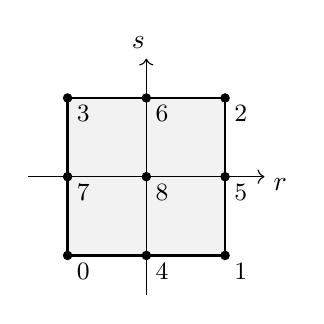
\begin{tikzpicture}
%\draw[step=0.5cm,gray,very thin] (0,0) grid (4,4); 
\draw[fill=gray!10,gray!10](1,1) rectangle (3,3);
\draw[thick] (1,1)--(3,1)--(3,3)--(1,3)--cycle;
\draw [->] (0.5,2) -- (3.5,2);
\draw [->] (2,0.5) -- (2,3.5);
\node[] at (3.7,1.9) {$r$};
\node[] at (1.9,3.7) {$s$};
\draw[black,fill=black] (1,1)   circle (1.5pt);
\draw[black,fill=black] (1,2)   circle (1.5pt);
\draw[black,fill=black] (1,3)   circle (1.5pt);
\draw[black,fill=black] (2,1)   circle (1.5pt);
\draw[black,fill=black] (2,2)   circle (1.5pt);
\draw[black,fill=black] (2,3)   circle (1.5pt);
\draw[black,fill=black] (3,1)   circle (1.5pt);
\draw[black,fill=black] (3,2)   circle (1.5pt);
\draw[black,fill=black] (3,3)   circle (1.5pt);
\node[] at (1.2,0.8) {\small $0$};
\node[] at (2.2,0.8) {\small $4$};
\node[] at (3.2,0.8) {\small $1$};
\node[] at (1.2,1.8) {\small $7$};
\node[] at (2.2,1.8) {\small $8$};
\node[] at (3.2,1.8) {\small $5$};
\node[] at (1.2,2.8) {\small $3$};
\node[] at (2.2,2.8) {\small $6$};
\node[] at (3.2,2.8) {\small $2$};
\end{tikzpicture}
\end{center}



\[
\vec{\bN}(r,s) 
=
\left(
\begin{array}{c}
\bN_1(r,s) \\ 
\bN_2(r,s) \\
\bN_3(r,s) \\
\bN_4(r,s) \\
\bN_5(r,s) \\
\bN_6(r,s) \\
\bN_7(r,s) \\
\bN_8(r,s) \\
\bN_9(r,s) 
\end{array}
\right)
=
\left(
\begin{array}{c}
\bN_1(r) \bN_1(s) \\
\bN_2(r) \bN_1(s) \\
\bN_3(r) \bN_1(s) \\
\bN_1(r) \bN_2(s) \\
\bN_2(r) \bN_2(s) \\
\bN_3(r) \bN_2(s) \\
\bN_1(r) \bN_3(s) \\
\bN_2(r) \bN_3(s) \\
\bN_3(r) \bN_3(s) 
\end{array}
\right)
=
\left(
\begin{array}{c}
 \frac{1}{2}r(r-1)  \frac{1}{2}s(s-1)\\
     (1-r^2)        \frac{1}{2}s(s-1)\\
 \frac{1}{2}r(r+1)  \frac{1}{2}s(s-1)\\
 \frac{1}{2}r(r-1)  (1-s^2)\\
     (1-r^2)        (1-s^2)
 \frac{1}{2}r(r+1)  (1-s^2)\\
 \frac{1}{2}r(r-1)  \frac{1}{2}s(s+1)\\
     (1-r^2)        \frac{1}{2}s(s+1)\\
 \frac{1}{2}r(r+1)  \frac{1}{2}s(s+1)\\
\end{array}
\right)
\]
The mass matrix on the reference element is then
\[
{\bm M}^e =
\iint_\square
\left(
\begin{array}{ccccccccc}
\bN_1 \bN_1 & \bN_1 \bN_2 & \bN_1 \bN_3 & \bN_1 \bN_4 & \bN_1 \bN_5 & \bN_1 \bN_6 & \bN_1 \bN_7 & \bN_1 \bN_8 & \bN_1 \bN_9 \\ 
\bN_2 \bN_1 & \bN_2 \bN_2 & \bN_2 \bN_3 & \bN_2 \bN_4 & \bN_2 \bN_5 & \bN_2 \bN_6 & \bN_2 \bN_7 & \bN_2 \bN_8 & \bN_2 \bN_9 \\ 
\dots \\
\bN_9 \bN_1 & \bN_9 \bN_2 & \bN_9 \bN_3 & \bN_9 \bN_4 & \bN_9 \bN_5 & \bN_9 \bN_6 & \bN_9 \bN_7 & \bN_9 \bN_8 & \bN_9 \bN_9 
\end{array}
\right)
dr ds
\]
with for example\footnote{Thank you WolframAlpha again!}
\begin{eqnarray}
\iint_\square \bN_1(r,s) \bN_1(r,s) \; drds &=&  \frac{16}{225} \\
\iint_\square \bN_1(r,s) \bN_2(r,s) \; drds &=& \frac{8}{225} \\ 
\iint_\square \bN_1(r,s) \bN_3(r,s) \; drds &=&  -\frac{4}{225} \\
\iint_\square \bN_1(r,s) \bN_8(r,s) \; drds &=&  \frac{-2}{225} \\
\iint_\square \bN_1(r,s) \bN_9(r,s) \; drds &=&  \frac{1}{225} \\
\iint_\square \bN_5(r,s) \bN_5(r,s) \; drds &=&  \frac{256}{225} \\
\end{eqnarray}

In \stone~107, we find for a 3x2 mesh on domain 6x4:
\begin{verbatim}
M = 
[[ 16.   8.  -4.   8.   4.  -2.  -4.  -2.   1.]
 [  8.  64.   8.   4.  32.   4.  -2. -16.  -2.]
 [ -4.   8.  16.  -2.   4.   8.   1.  -2.  -4.]
 [  8.   4.  -2.  64.  32. -16.   8.   4.  -2.]
 [  4.  32.   4.  32. 256.  32.   4.  32.   4.]
 [ -2.   4.   8. -16.  32.  64.  -2.   4.   8.]
 [ -4.  -2.   1.   8.   4.  -2.  16.   8.  -4.]
 [ -2. -16.  -2.   4.  32.   4.   8.  64.   8.]
 [  1.  -2.  -4.  -2.   4.   8.  -4.   8.  16.]] / 225
\end{verbatim}







\newpage
%------------------------------------------------------------------------
\section{3d hexahedra}

%---------------------------
\subsection{Linear cuboid elements $Q_1$ - $\K$ and $\G$ matrices}

We here assume that each element is a cuboid\footnote{\url{https://en.wikipedia.org/wiki/Cuboid}}. 
We set the domain size to $L_x=4$, $L_x=3$ and $L_z=2$, with $nelx=4$, 
$nely=3$ and $nelz=2$. Here again the viscosity is set to $\eta=1$ so that 
we find that 
\begin{footnotesize}
\[
\K_{el}=\frac{1}{8\cdot 9}
\left(
\begin{array}{cccccccccccccccccccccccc}
32&   6&   6&  -8&  -6&  -6& -10&  -6&  -3&   4&   6&   3&   4&   3&    6& -10&  -3&  -6&  -8&  -3&  -3&  -4&   3&   3\\
 6&  32&   6&   6&   4&   3&  -6& -10&  -3&  -6&  -8&  -6&   3&   4&    6&   3&  -4&   3&  -3&  -8&  -3&  -3& -10&  -6\\
 6&   6&  32&   6&   3&   4&   3&   3&  -4&   3&   6&   4&  -6&  -6&   -8&  -6&  -3& -10&  -3&  -3&  -8&  -3&  -6& -10\\
-8&   6&   6&  32&  -6&  -6&   4&  -6&  -3& -10&   6&   3& -10&   3&    6&   4&  -3&  -6&  -4&  -3&  -3&  -8&   3&   3\\
-6&   4&   3&  -6&  32&   6&   6&  -8&  -6&   6& -10&  -3&  -3&  -4&    3&  -3&   4&   6&   3& -10&  -6&   3&  -8&  -3\\
-6&   3&   4&  -6&   6&  32&  -3&   6&   4&  -3&   3&  -4&   6&  -3&  -10&   6&  -6&  -8&   3&  -6& -10&   3&  -3&  -8\\
10&  -6&   3&   4&   6&  -3&  32&   6&  -6&  -8&  -6&   6&  -8&  -3&    3&  -4&   3&  -3&   4&   3&  -6& -10&  -3&   6\\
-6& -10&   3&  -6&  -8&   6&   6&  32&  -6&   6&   4&  -3&  -3&  -8&    3&  -3& -10&   6&   3&   4&  -6&   3&  -4&  -3\\
-3&  -3&  -4&  -3&  -6&   4&  -6&  -6&  32&  -6&  -3&   4&   3&   3&   -8&   3&   6& -10&   6&   6&  -8&   6&   3& -10\\
 4&  -6&   3& -10&   6&  -3&  -8&   6&  -6&  32&  -6&   6&  -4&  -3&    3&  -8&   3&  -3& -10&   3&  -6&   4&  -3&   6\\
 6&  -8&   6&   6& -10&   3&  -6&   4&  -3&  -6&  32&  -6&   3& -10&    6&   3&  -8&   3&  -3&  -4&  -3&  -3&   4&  -6\\
 3&  -6&   4&   3&  -3&  -4&   6&  -3&   4&   6&  -6&  32&  -3&   6&  -10&  -3&   3&  -8&  -6&   3& -10&  -6&   6&  -8\\
 4&   3&  -6& -10&  -3&   6&  -8&  -3&   3&  -4&   3&  -3&  32&   6&   -6&  -8&  -6&   6& -10&  -6&   3&   4&   6&  -3\\
 3&   4&  -6&   3&  -4&  -3&  -3&  -8&   3&  -3& -10&   6&   6&  32&   -6&   6&   4&  -3&  -6& -10&   3&  -6&  -8&   6\\
 6&   6&  -8&   6&   3& -10&   3&   3&  -8&   3&   6& -10&  -6&  -6&   32&  -6&  -3&   4&  -3&  -3&  -4&  -3&  -6&   4\\
10&   3&  -6&   4&  -3&   6&  -4&  -3&   3&  -8&   3&  -3&  -8&   6&   -6&  32&  -6&   6&   4&  -6&   3& -10&   6&  -3\\
-3&  -4&  -3&  -3&   4&  -6&   3& -10&   6&   3&  -8&   3&  -6&   4&   -3&  -6&  32&  -6&   6&  -8&   6&   6& -10&   3\\
-6&   3& -10&  -6&   6&  -8&  -3&   6& -10&  -3&   3&  -8&   6&  -3&    4&   6&  -6&  32&   3&  -6&   4&   3&  -3&  -4\\
-8&  -3&  -3&  -4&   3&   3&   4&   3&   6& -10&  -3&  -6& -10&  -6&   -3&   4&   6&   3&  32&   6&   6&  -8&  -6&  -6\\
-3&  -8&  -3&  -3& -10&  -6&   3&   4&   6&   3&  -4&   3&  -6& -10&   -3&  -6&  -8&  -6&   6&  32&   6&   6&   4&   3\\
-3&  -3&  -8&  -3&  -6& -10&  -6&  -6&  -8&  -6&  -3& -10&   3&   3&   -4&   3&   6&   4&   6&   6&  32&   6&   3&   4\\
-4&  -3&  -3&  -8&   3&   3& -10&   3&   6&   4&  -3&  -6&   4&  -6&   -3& -10&   6&   3&  -8&   6&   6&  32&  -6&  -6\\
 3& -10&  -6&   3&  -8&  -3&  -3&  -4&   3&  -3&   4&   6&   6&  -8&   -6&   6& -10&  -3&  -6&   4&   3&  -6&  32&   6\\
 3&  -6& -10&   37  -3&  -8&   6&  -3& -10&   6&  -6&  -8&  -3&   6&    4&  -3&   3&  -4&  -6&   3&   4&  -6&   6&  32
\end{array}
\right)
\]
\end{footnotesize}
and 
\begin{scriptsize}
\[
\G_{el}=\frac{1}{2\cdot 9}
\left(
\begin{array}{c}
 1\\
 1\\
 1\\
-1\\
 1\\
 1\\
-1\\
-1\\
 1\\
 1\\
-1\\
 1\\
 1\\
 1\\
-1\\
-1\\
 1\\
-1\\
-1\\
-1\\
-1\\
 1\\
-1\\
-1
\end{array}
\right)
\]
\end{scriptsize}


\newpage
%---------------------------------------
\section{Triangles: linear elements} \label{ss:tle}


\subsection{linear elements $P_1$} 

We start from the linear basis functions in the reference triangle given as a function of $r,s$:
\begin{eqnarray}
\bN_1(r,s) &=& 1-r-s \nn\\
\bN_2(r,s) &=& r \nn\\
\bN_3(r,s) &=& s \nn
\end{eqnarray}
and their derivatives:
\begin{eqnarray}
\partial_r \bN_1(r,s) &=& -1 \nonumber\\
\partial_r \bN_2(r,s) &=& 1 \nonumber\\
\partial_r \bN_3(r,s) &=& 0 \nonumber\\
\partial_s \bN_1(r,s) &=& -1 \nonumber\\
\partial_s \bN_2(r,s) &=& 0\nonumber\\
\partial_s \bN_3(r,s) &=& 1\nonumber
\end{eqnarray}
We wish to compute the integral of a function $f(x,y)$ over the triangle by means of a change of variables
$(x,y)\rightarrow (r,s)$:
\begin{eqnarray}
\iint f(x,y) dx dy 
&=& \iint f(x(r,s),y(r,s)) \left| \frac{\partial (x,y)}{\partial (r,s) } \right|  dr ds \nonumber\\
&=& \iint f(x(r,s),y(r,s)) 
\left| 
\begin{array}{cc}
\partial x/\partial r & \partial x/\partial s \\ \\
\partial y/\partial r & \partial y/\partial s 
\end{array}
\right|  dr ds 
\end{eqnarray}
From 
\begin{eqnarray}
x(r,s)&=&\sum_{i=1}^3 \bN_i(r,s) x_i = (1-r-s)x_1 + rx_2 + sx_3 = (x_2-x_1)r+(x_3-x_1)s+x_1  \nn\\
y(r,s)&=&\sum_{i=1}^3 \bN_i(r,s) y_i = (1-r-s)y_1 + ry_2 + sy_3 = (y_2-y_1)r+(y_3-y_1)s+y_1  \nn
\end{eqnarray}
we can write
\begin{eqnarray}
\frac{\partial x}{\partial r}(r,s)
&=&\sum_{i=1}^3 \frac{\partial \bN_i}{\partial r} x_i
=\frac{\partial \bN_1}{\partial r} x_1+\frac{\partial \bN_2}{\partial r} x_2+\frac{\partial \bN_3}{\partial r} x_3
=- x_1+ x_2 \nonumber\\
\frac{\partial x}{\partial s}(r,s)
&=&\sum_{i=1}^3 \frac{\partial \bN_i}{\partial s} x_i
=\frac{\partial \bN_1}{\partial s} x_1+\frac{\partial \bN_2}{\partial s} x_2+\frac{\partial \bN_3}{\partial s} x_3
=- x_1+ x_3
\nonumber\\
\frac{\partial y}{\partial r}(r,s)
&=&\sum_{i=1}^3 \frac{\partial \bN_i}{\partial r} y_i
=\frac{\partial \bN_1}{\partial r} x_1+\frac{\partial \bN_2}{\partial r} x_2+\frac{\partial \bN_3}{\partial r} y_3
=- y_1+ y_2
\nonumber\\
\frac{\partial y}{\partial s}(r,s)
&=&\sum_{i=1}^3 \frac{\partial \bN_i}{\partial s} y_i
=\frac{\partial \bN_1}{\partial s} y_1+\frac{\partial \bN_2}{\partial s} y_2+\frac{\partial \bN_3}{\partial s} y_3
=- y_1+ y_3
\end{eqnarray}
Then 
\[
\left| 
\begin{array}{cc}
\partial x/\partial r & \partial x/\partial s \\ \\
\partial y/\partial r & \partial y/\partial s 
\end{array}
\right|  
=
\left| 
\begin{array}{cc}
- x_1+ x_2 & - x_1+ x_3 \\
- y_1+ y_2 & - y_1+ y_3 
\end{array}
\right|  
=
(x_2-x_1)(y_3-y_1)-(y_2-y_1)(x_3-x_1)
= 2S
\]
where $S$ is the area of the triangle and which is independent of $(r,s)$.
Looking at the reference element, we find that when $r$ goes from 0 to 1, 
$s$ can only take values between 0 and $1-r$.
\begin{center}
\includegraphics[width=4cm]{images/elemental_mat/triangle}
\end{center}
Then the bounds of the integrals are simply: 
\begin{eqnarray}
\iint_\triangle f(x,y) dx dy &=& 2S \int_0^{1} \left(\int_0^{1-r} f(x(r,s),y(r,s))  ds \right) dr 
\end{eqnarray}
and the mass matrix is given by
\begin{eqnarray}
{\bm M}_e 
&=& 2S \int_{0}^1 \left[ \int_{0}^{1-r}
\left(
\begin{array}{ccc}
(1-r-s)^2 & (1-r-s)r & (1-r-s)s \\
(1-r-s)r & r^2 & rs \\
(1-r-s)s & rs & s^2 
\end{array}
\right)
 ds \right] dr \\
&=& 
2S \int_{0}^1 
\left(
\begin{array}{ccc}
\int_0^{1-r} (1-r-s)^2 ds &\int_0^{1-r} (1-r-s)r ds& \int_0^{1-r} (1-r-s)s ds \\ \\
\int_0^{1-r} (1-r-s)r ds  &\int_0^{1-r} r^2 ds     & \int_0^{1-r} rs ds \\ \\
\int_0^{1-r} (1-r-s)s ds  &\int_0^{1-r} rs ds      & \int_0^{1-r} s^2 ds
\end{array}
\right)
 dr \\
&=& 
2S
\left(
\begin{array}{ccc}
1/12 & 1/24 & 1/24 \\
1/24 & 1/12 & 1/24 \\
1/24 & 1/24 & 1/12
\end{array}
\right)
\\
&=&
\frac{S}{12}
\left(
\begin{array}{ccc}
2 & 1 & 1 \\
1 & 2 & 1 \\
1 & 1 & 2
\end{array}
\right)
\end{eqnarray}
This is Eq.(4.10e) of \textcite{li06}. 
Also note that in the context of the heat transport equation this matrix is multiplied 
by $\rho C_p$ (all under the assumption that these coefficients are constant 
over the whole element).

%We will then compute the ${\bm J}_x$ and ${\bm J}_y$ matrices\footnote{Nobody 
%knows what these matrices are for ... needs to be looked into.}.
The basis functions can also directly be expressed in the $(x,y)$ coordinate system
(see for example Section~\ref{ss:p1}):
\begin{eqnarray}
\bN_1(x,y) &=& \frac{1}{2S} \left( x_2y_3-x_3y_2+(y_2-y_3)x+(x_3-x_2)y   \right) \nn\\
\bN_2(x,y) &=& \frac{1}{2S} \left( x_3y_1-x_1y_3+(y_3-y_1)x+(x_1-x_3)y   \right) \nn\\
\bN_3(x,y) &=& \frac{1}{2S} \left( x_1y_2-x_2y_1+(y_1-y_2)x+(x_2-x_1)y   \right) \nn
\end{eqnarray}
where $S$ is the area of the element.
We then have 
\begin{eqnarray}
\partial_x \bN_1(x,y) &=& \frac{1}{2S}  (y_2-y_3) = \frac{1}{2S} y_{23} \nn\\
\partial_x \bN_2(x,y) &=& \frac{1}{2S}  (y_3-y_1) = \frac{1}{2S} y_{31} \nn\\
\partial_x \bN_3(x,y) &=& \frac{1}{2S}  (y_1-y_2) = \frac{1}{2S} y_{12} \nn\\
\partial_y \bN_1(x,y) &=& \frac{1}{2S}  (x_3-x_2) = \frac{1}{2S} y_{32} \nn\\
\partial_y \bN_2(x,y) &=& \frac{1}{2S}  (x_1-x_3) = \frac{1}{2S} y_{13} \nn\\
\partial_y \bN_3(x,y) &=& \frac{1}{2S}  (x_2-x_1) = \frac{1}{2S} y_{21} \nn
\end{eqnarray}
where we have introduced the notation $x_{ij}=x_i-x_j$ and $y_{ij}=y_i-y_j$.

%We start with
%\begin{eqnarray}
%{\bm J}_x
%&=& \iint_\triangle  \partial_x \vec{\bN}^T \vec{\bN} dV \nn\\
%&=&  \iint_\triangle 
%\left(
%\begin{array}{c}
%\frac{1}{2S}(y_2-y_3) \\
%\frac{1}{2S}(y_3-y_1) \\
%\frac{1}{2S}(y_1-y_2)
%\end{array}
%\right)
%\left(
%\begin{array}{ccc}
%N_1(x,y) & N_2(x,y) & N_3(x,y) 
%\end{array}
%\right) dx dy \nn\\
%&=& \frac{1}{2S} 
%\left(
%\begin{array}{ccc}
%y_{23} \iint_\triangle \bN_1 dx dy & y_{23} \iint_\triangle \bN_2 dx dy & y_{23} \iint_\triangle \bN_3 dx dy \\
%y_{31} \iint_\triangle \bN_1 dx dy & y_{31} \iint_\triangle \bN_2 dx dy & y_{31} \iint_\triangle \bN_3 dx dy \\
%y_{12} \iint_\triangle \bN_1 dx dy & y_{12} \iint_\triangle \bN_2 dx dy & y_{12} \iint_\triangle \bN_3 dx dy 
%\end{array}
%\right) 
%\end{eqnarray}
%We then need to compute
%\begin{eqnarray}
%\iint_\triangle \bN_1(x,y) dx dy 
%&=& 2S \int_0^{1} \left(\int_0^{1-r} \bN_1(x(r,s),y(r,s))  ds \right) dr \nonumber\\ 
%&=& 2S \int_0^{1} \left(\int_0^{1-r} (1-r-s)  ds \right) dr \nonumber\\ 
%&=& 2S \frac{1}{6} \label{eq:elmats:1}\\ 
%\iint_\triangle \bN_2(x,y) dx dy 
%&=& 2S \int_0^{1} \left(\int_0^{1-r} \bN_2(x(r,s),y(r,s))  ds \right) dr \nonumber\\ 
%&=& 2S \int_0^{1} \left(\int_0^{1-r} r  ds \right) dr \nonumber\\ 
%&=& 2S \frac{1}{6} \label{eq:elmats:2}\\ 
%\iint_\triangle \bN_3(x,y) dx dy 
%&=& 2S \int_0^{1} \left(\int_0^{1-r} \bN_3(x(r,s),y(r,s))  ds \right) dr \nonumber\\ 
%&=& 2S \int_0^{1} \left(\int_0^{1-r} s  ds \right) dr \nonumber\\ 
%&=& 2S \frac{1}{6} \label{eq:elmats:3} 
%\end{eqnarray}
%\todo[inline]{verify!! FOR REAL 2025}
%Finally:
%\[
%{\bm J}_x
%=
%\frac{1}{6}
%%\left(
%\begin{array}{ccc}
%y_{23} & y_{23} & y_{23} \\ 
%y_{31} & y_{31} & y_{31} \\ 
%y_{12} & y_{12} & y_{12}  
%\end{array}
%\right) 
%\]
%Likewise
%\begin{eqnarray}
%{\bm J}_y
%&=& \iint_\triangle  \partial_y \vec{\bN}^T \vec{\bN} dV \nn\\
%&=&  \iint_\triangle 
%\left(
%\begin{array}{c}
%\frac{1}{2S}(x_3-x_2) \\
%\frac{1}{2S}(x_1-x_3) \\
%\frac{1}{2S}(x_2-x_1)
%\end{array}
%\right)
%\left(
%\begin{array}{ccc}
%\bN_1(x,y) & \bN_2(x,y) & \bN_3(x,y) 
%\end{array}
%\right) dx dy \nn\\
%&=&
%\frac{1}{6}
%\left(
%\begin{array}{ccc}
%x_{32} & x_{32} & x_{32} \\ 
%x_{13} & x_{13} & x_{13} \\ 
%x_{21} & x_{21} & x_{21}  
%\end{array}
%\right) 
%\end{eqnarray}

We now turn to the diffusion $\K_d$ matrices.
The gradient matrix ${\bm B}$ is given by 
\[
{\bm B} = 
\left(
\begin{array}{ccc}
\partial_x \bN_1 & \partial_x \bN_2 & \partial_x \bN_3 \\
\partial_y \bN_1 & \partial_y \bN_2 & \partial_y \bN_3 \\
\end{array}
\right)
=
\frac{1}{2S}
\left(
\begin{array}{ccc}
y_{23} & y_{31} & y_{12} \\
x_{32} & x_{13} & x_{21}
\end{array}
\right)
\]
then 
\[
{\bm K}_d 
= \iint_\triangle {\bm B}^T k {\bm B} \; dV
= \iint_\triangle \frac{k}{4S^2}
\left(
\begin{array}{cc}
y_{23} & x_{32} \\ 
y_{31} & x_{13} \\
y_{12} & x_{21}
\end{array}
\right)
\cdot
\left(
\begin{array}{ccc}
y_{23} & y_{31} & y_{12} \\
x_{32} & x_{13} & x_{21}
\end{array}
\right)
\; dV
\]
If the heat conductivity $k$ is constant within the element, then 
the integrand in the expression above is constant with respect to the 
integration and since $\iint_\triangle dV = S$ we then obtain:
\[
\K_d 
= \frac{k}{4S}
\left(
\begin{array}{cc}
y_{23} & x_{32} \\ 
y_{31} & x_{13} \\
y_{12} & x_{21}
\end{array}
\right)
\cdot
\left(
\begin{array}{ccc}
y_{23} & y_{31} & y_{12} \\
x_{32} & x_{13} & x_{21}
\end{array}
\right)
\]
or
\[
\boxed{
\K_d 
= \frac{k}{4S}
\left(
\begin{array}{ccc}
y_{23}y_{23} + x_{32}x_{32} & y_{23}y_{31} + x_{32}x_{13} & y_{23}y_{12} + x_{32}x_{21}  \\ 
y_{31}y_{23} + x_{13}x_{32} & y_{31}y_{31} + x_{13}x_{13} & y_{31}y_{12} + x_{13}x_{21}  \\ 
y_{12}y_{23} + x_{21}x_{32} & y_{12}y_{31} + x_{21}x_{13} & y_{12}y_{12} + x_{21}x_{21} 
\end{array}
\right)
}
\]



Turning now to the advection matrix
\begin{eqnarray}
\K_a 
&=& \iint_\triangle \vec{\bN}^T  \; \vec{\upnu}\cdot {\bm B} \; dV \nn\\
&=& \iint_\triangle \vec{\bN}^T(x,y) \; \vec{\upnu}(x,y) \cdot {\bm B}(x,y) \; dx dy \nn
\end{eqnarray}

If the velocity is constant within the element (which is rarely the case) then 
this expression can be integrated exactly. If not, a quadrature rule must be used.

Let us assume that velocity is indeed constant inside the element. Then
$\vec{\upnu}(x,y)=\vec\upnu_0=(u_0,v_0)$ and
\begin{eqnarray}
\K_a 
&=& \iint_\triangle \vec{\bN}^T(x,y) \; \vec{\upnu}_0 \cdot {\bm B}(x,y) \; dx dy \nn\\
&=& \iint_\triangle
\left(
\begin{array}{c}
\bN_1(x,y) \\
\bN_2(x,y) \\
\bN_3(x,y) 
\end{array}
\right)
\;
(u_0,v_0)
\cdot
\frac{1}{2S}
\left(
\begin{array}{ccc}
y_{23} & y_{31} & y_{12} \\
x_{32} & x_{13} & x_{21}
\end{array}
\right) \; dxdy \nn\\
&=& 
\frac{1}{2S}
\iint_\triangle
\left(
\begin{array}{c}
\bN_1(x,y) \\
\bN_2(x,y) \\
\bN_3(x,y) 
\end{array}
\right)
\left(
\begin{array}{ccc}
u_0 y_{23}+ v_0 x_{32}  &
u_0 y_{31}+ v_0 x_{13}  &
u_0 y_{12}+ v_0 x_{21}  
\end{array}
\right)
\; dx dy \nn
\end{eqnarray}
Since the terms in the second vector is independent of $x,y$ we will need to compute
\[
\iint_\triangle \bN_1(x,y) dxdy, \qquad 
\iint_\triangle \bN_2(x,y) dxdy, \qquad \text{and} \quad 
\iint_\triangle \bN_3(x,y) dxdy. 
\]
We have established that for any function $f(x,y)$ we have
\[
\iint_\triangle f(x,y) dx dy = 2S \int_0^{1} \left(\int_0^{1-r} f(x(r,s),y(r,s))  ds \right) dr 
\]
Then
\begin{eqnarray}
\iint_\triangle \bN_1(x,y) dxdy 
&=& 2S \int_0^{1} \left(\int_0^{1-r} \bN_1(r,s)  ds \right) dr \nn\\
&=& 2S \int_0^{1} \left(\int_0^{1-r} (1-r-s)  ds \right) dr \nn\\
&=& 2S \int_0^{1} \left[ (1-r)s -\frac12 s^2)   \right]_0^{1-r} dr \nn\\
&=& 2S \int_0^{1} \left( (1-r)^2 -\frac12 (1-r)^2   \right) dr \nn\\
&=& 2S \int_0^{1} \frac12 (1-r)^2  dr \nn\\
&=& 2S \frac16 \nn\\
\iint_\triangle \bN_2(x,y) dxdy 
&=& 2S \int_0^{1} \left(\int_0^{1-r} \bN_2(r,s)  ds \right) dr \nn\\
&=& 2S \int_0^{1} \left(\int_0^{1-r} r  ds \right) dr \nn\\
&=& 2S \int_0^{1} r (1-r) dr \nn\\
&=& 2S \frac16 \nn\\
\iint_\triangle \bN_3(x,y) dxdy 
&=& 2S \int_0^{1} \left(\int_0^{1-r} \bN_3(r,s)  ds \right) dr \nn\\
&=& 2S \int_0^{1} \left(\int_0^{1-r} s  ds \right) dr \nn\\
&=& 2S \int_0^{1} [\frac12 s^2]_0^{1-r}  dr \nn\\
&=& 2S \frac12 \int_0^{1} (1-r)^2  dr \nn\\
&=& 2S \frac16 \nn
\end{eqnarray}
In the end
\[
\boxed{
\K_a
= \frac16
\left(
\begin{array}{ccc}
u_0 y_{23}+ v_0 x_{32}  & u_0 y_{31}+ v_0 x_{13}  & u_0 y_{12}+ v_0 x_{21}  \\
u_0 y_{23}+ v_0 x_{32}  & u_0 y_{31}+ v_0 x_{13}  & u_0 y_{12}+ v_0 x_{21}  \\
u_0 y_{23}+ v_0 x_{32}  & u_0 y_{31}+ v_0 x_{13}  & u_0 y_{12}+ v_0 x_{21}  
\end{array}
\right)
}
\]
This expression was tested against a numerically integrated approach in 
\stone~45 (simply set \lstinline{test=True} in the code). 

If the element under consideration is the reference element, we 
we have

\begin{eqnarray}
\K_a 
&=& 
\int_0^{1} \left[ \int_0^{1-r}
\left(
\begin{array}{c}
\bN_1(r,s) \\
\bN_2(r,s) \\
\bN_3(r,s) 
\end{array}
\right)
\;
(u_0,v_0)
\cdot
\left(
\begin{array}{ccc}
-1 & 1 & 0 \\
-1 & 0 & 1
\end{array}
\right) ds \right] dr  \nn\\
&=&
\int_0^{1} \left[ \int_0^{1-r}
\left(
\begin{array}{c}
\bN_1(r,s) \\
\bN_2(r,s) \\
\bN_3(r,s) 
\end{array}
\right)
(-u_0-v_0 , u_0 , v_0) \;
ds \right] dr \nn\\
&=& \frac16
\left(
\begin{array}{ccc}
-u_0 - v_0   & u_0   &  v_0   \\
-u_0 - v_0   & u_0   &  v_0   \\
-u_0 - v_0   & u_0   &  v_0   
\end{array}
\right)
\end{eqnarray}















\newpage
\[
{\bm C}_1
=\int_{\partial\Omega_1} \vec{N}^T(x,y) \vec{N}(x,y) d\Gamma
\]
The edge $\partial\Omega_1$ is bounded by the coordinates of nodes $x_1,y_1$
and $x_2,y_2$. This segment can be parameterised by $t\in[0,1]$:
\[
\vec{r}(t) = (1-t)\left(\begin{array}{c} x_1 \\ y_1 \end{array} \right) + 
t \left(\begin{array}{c} x_2 \\ y_2 \end{array} \right)
=
\left(\begin{array}{c} (x_2-x_1)t +x_1 \\ (y_2-y_1)t+y_1 \end{array} \right) 
\]

Let us assume that $C$ is a smooth curve and that it is given by the 
parametric equations $x=h(t)$, $y=g(t)$ and $a\leq t \leq b$. The line integral 
of a function $f(x,y)$ over $C$ is computed as follows. 
\[
\int_C f(x,y) ds = \int_a^b f(h(t),g(t)) \sqrt{\left(\frac{dx}{dt}\right)^2 + \left(\frac{dy}{dt}\right)^2} dt
\]
In our case $dx/dt=x_2-x_1$ and $dy/dt=y_2-y_1$ so 
\[
\sqrt{\left(\frac{dx}{dt}\right)^2 + \left(\frac{dy}{dt}\right)^2}
=\sqrt{(x_2-x_1)^2+(y_2-y_1)^2} = L_1
\]
Then 
\begin{eqnarray}
{\bm C}_1
&=&\int_{\partial\Omega_1} \vec{N}^T(x,y) \vec{N}(x,y) d\Gamma \nn\\
&=&
\left(
\begin{array}{ccc}
\int_{\partial\Omega_1} N_1(x,y)N_1(x,y) d\Gamma & 
\int_{\partial\Omega_1} N_1(x,y)N_2(x,y) d\Gamma &
\int_{\partial\Omega_1} N_1(x,y)N_3(x,y) d\Gamma \\
\int_{\partial\Omega_1} N_2(x,y)N_1(x,y) d\Gamma & 
\int_{\partial\Omega_1} N_2(x,y)N_2(x,y) d\Gamma &
\int_{\partial\Omega_1} N_2(x,y)N_3(x,y) d\Gamma \\
\int_{\partial\Omega_1} N_3(x,y)N_1(x,y) d\Gamma & 
\int_{\partial\Omega_1} N_3(x,y)N_2(x,y) d\Gamma &
\int_{\partial\Omega_1} N_3(x,y)N_3(x,y) d\Gamma 
\end{array}
\right) \nn\\
&=&
L_1
\left(
\begin{array}{ccc}
\int_{0}^1 N_1(x(t),y(t))N_1(x(t),y(t)) dt & 
\int_{0}^1 N_1(x(t),y(t))N_2(x(t),y(t)) dt &
\int_{0}^1 N_1(x(t),y(t))N_3(x(t),y(t)) dt \\\\
\int_{0}^1 N_2(x(t),y(t))N_1(x(t),y(t)) dt & 
\int_{0}^1 N_2(x(t),y(t))N_2(x(t),y(t)) dt &
\int_{0}^1 N_2(x(t),y(t))N_3(x(t),y(t)) dt \\\\
\int_{0}^1 N_3(x(t),y(t))N_1(x(t),y(t)) dt & 
\int_{0}^1 N_3(x(t),y(t))N_2(x(t),y(t)) dt &
\int_{0}^1 N_3(x(t),y(t))N_3(x(t),y(t)) dt
\end{array}
\right) \nn\\
\end{eqnarray}

We are about to compute the individual terms of the matrix
one by one but we will need:
\begin{eqnarray}
S
&=& \frac{1}{2} [(x_1-x_3)(y_2-y_3)-(x_2-x_3)(y_1-y_3)]  \nn\\
&=&  \frac{1}{2} [x_1y_2 -x_1y_3 -x_3y_2 + x_3y_3 -x_2y_1 + x_2y_3 + x_3y_1 - x_3y_3] \nn\\
&=&  \frac{1}{2} [x_1y_2 -x_1y_3 -x_3y_2 -x_2y_1 + x_2y_3 + x_3y_1 ] \nn\\
\end{eqnarray}
and 
\begin{eqnarray}
N_1(x(t),y(t)) 
&=&\frac{1}{2S} [  x_2y_3-x_3y_2+(y_2-y_3)x(t)+(x_3-x_2)y(t) ] \nn\\
&=&\frac{1}{2S} [  x_2y_3-x_3y_2+y_{23}(x_{21} t +x_1)  +x_{32}  (y_{21} t+y_1) ] \nn\\
&=&\frac{1}{2S} [ x_2y_3-x_3y_2 +y_{23}x_1+x_{32}y_1 + (y_{23}x_{21}+x_{32}y_{21}) t  ] \nn\\
&=&\frac{1}{2S} [ \underbrace{x_2y_3-x_3y_2 +x_1y_2-x_1y_3 +x_{3}y_1-x_2y_1}_{2S} \\ 
&& + (x_2y_2-x_1y_2-x_2y_3+x_1y_3 + x_3y_2 - x_3y_1 - x_2y_2 + x_2y_1  ) t  ]  \nn\\
&=&\frac{1}{2S} [ 2S - (\underbrace{x_1y_2+x_2y_3-x_1y_3 - x_3y_2 + x_3y_1 - x_2y_1}_{2S}  ) t  ]  \nn\\
&=&\frac{1}{2S} [ 2S - 2S  t  ] \nn\\
&=&1-t \\
N_2(x(t),y(t)) 
&=& \frac{1}{2S} [ x_3y_1-x_1y_3+(y_3-y_1)(x_{21} t +x_1)+(x_1-x_3)(y_{21} t+y_1)  ] \nn\\
&=& \frac{1}{2S} [ x_3y_1-x_1y_3+(y_3-y_1)x_1+(x_1-x_3)y_1 + (y_{31}x_{21}+x_{13}y_{21}) t ] \nn\\
&=& \frac{1}{2S} [ x_3y_1-x_1y_3+x_1y_3 -x_1y_1+ x_1y_1 -x_3y_1 + (y_{31}x_{21}+x_{13}y_{21}) t ] \nn\\
&=& \frac{1}{2S}   (y_{31}x_{21}+x_{13}y_{21}) t  \nn\\
&=& t \\ 
N_3(x(t),y(t)) 
&=& \frac{1}{2S} ( x_1y_2-x_2y_1+(y_1-y_2)x(t)+(x_2-x_1)y(t)   ) \nn\\
&=& \frac{1}{2S} ( x_1y_2-x_2y_1+(y_1-y_2)( x_{21} t +x_1 )+(x_2-x_1)(y_{21} t+y_1 )   ) \nn\\
&=& \frac{1}{2S} ( x_1y_2-x_2y_1+(y_1-y_2)x_1 +(x_2-x_1)y_1 + (y_{12}x_{21}+x_{21}y_{21})t  ) \nn\\
&=& \frac{1}{2S} ( x_1y_2-x_2y_1+x_1y_1-x_1y_2 +x_2y_1-x_1y_1 + (y_{12}x_{21}-x_{21}y_{12})t     ) \nn\\
&=& 0
\end{eqnarray}


then 

\begin{eqnarray}
\int_{0}^1 N_1(x(t),y(t))N_1(x(t),y(t)) dt 
&=& \int_{0}^1 (1-t)^2 dt = 1/3 \\ 
\int_{0}^1 N_1(x(t),y(t))N_2(x(t),y(t)) dt 
&=& \int_{0}^1 (1-t)t dt = 1/6 \\ 
\int_{0}^1 N_1(x(t),y(t))N_3(x(t),y(t)) dt
&=& 0 \\
\int_{0}^1 N_2(x(t),y(t))N_2(x(t),y(t)) dt 
&=& \int_{0}^1 t^2 dt = 1/3 \\ 
\int_{0}^1 N_2(x(t),y(t))N_3(x(t),y(t)) dt
&=& 0 \\
\int_{0}^1 N_3(x(t),y(t))N_3(x(t),y(t)) dt
&=& 0 
\end{eqnarray}
and finally 
\begin{eqnarray}
{\bm C}_1
&=&\int_{\partial\Omega_1} \vec{N}^T(x,y) \vec{N}(x,y) d\Gamma 
= \frac{L_1}{6}
\left(
\begin{array}{ccc}
2 & 1 & 0 \\
1 & 2 & 0 \\
0 & 0 & 0 
\end{array}
\right) \\
{\bm C}_2 &=&\int_{\partial\Omega_2} \vec{N}^T(x,y) \vec{N}(x,y) d\Gamma 
= \frac{L_2}{6}
\left(
\begin{array}{ccc}
0 & 0 & 0 \\
0 & 2 & 1 \\
0 & 1 & 2 
\end{array}
\right) \\
{\bm C}_3 &=&\int_{\partial\Omega_3} \vec{N}^T(x,y) \vec{N}(x,y) d\Gamma 
= \frac{L_3}{6}
\left(
\begin{array}{ccc}
2 & 0 & 1 \\
0 & 0 & 0 \\
1 & 0 & 2 
\end{array}
\right) 
\end{eqnarray}





 %%%%%
\chapter{Fun modelling} Because sometimes numerical modelling {\sl is} fun ...

\begin{center}
\includegraphics[width=8cm]{images/interesting/akds14}\\
{\small Clothes washing simulations \cite{akds14}}
\end{center}


\begin{center}
\includegraphics[width=8cm]{images/interesting/mega03}\\
{\small Pressures produced when penguins pooh—calculations on avian defaecation \cite{mega03}}
\end{center}


 %%%%%%%%%%%%%%%%%%%%%%%%%%%%%%%%%%%%%%%%%%%%%%%%%%%%%%%
\chapter{Working with Git from the terminal} \textbf{MIND YOURSELF: Working in a Mac OS, be carefull with case sensitive file names etc...}

In this appendix we summarize the most important commands one should and remember while working with github. After creating an account one can 'fork' a repository (repo) in the online environment. This repository is a copy from the master directory of the developer and should not be used to adapt or change, as changes from the developer (updates) should be obtained in this 'fork', or as it could also be called; your master branch. 
  
In order to be able to work within a repository, for instance, to run and compile different programs, you should have you own branch of the repository in which YOU CAN make changes. The following commands should be used to make, copy and publish your own version of the repo to your local device and the online github environment.

\begin{center}
\begin{tabular}{p{6cm}|p{9cm}}
\textbf{command} &  \textbf{what it does} \\
\hline
  git branch & shows all branches of your repository and highlights the one you're in. \\
  git checkout -b \textless my\_own\_branch\textgreater & This makes your own branch called "my\_own\_branch". \\
  git push origin \textless my\_own\_branch\textgreater & This pushes your own, local, branch to as a second branch in the online repo of github. \\
  git checkout \textless name\textgreater & changing the branch your working in (e.g. master or my\_own\_branch). Or replace the name with a hyphen to switch to the last branch.\\
  git branch -d \textless my\_own\_branch\textgreater & Delete your local branch. \\
  \end{tabular}
\end{center}

  The following commands should be used in order to update your own local branches from updates made by somewhere else (upstream/master is the main repository). One should do this for the local master branch and, where possible as well for the different local branches you have committed changes to already. 

  
\begin{center}
\begin{tabular}{p{6cm}|p{9cm}}
\textbf{command} &  \textbf{what it does} \\
\hline
git checkout master & To make sure you are in the right branch \\
  git fetch upstream & to fetch updates from upstream repositories to you own local branch (e.g. to update your master branch. \\
  git merge upstream/master & Command to update the branch with the fethched repo from 'upstream'. \\
  git push origin master & To level your own online repository again with the one on your local drive (and thus the one upstream). \\
  git checkout \textless my\_own\_branch\textgreater & To switch to your own adapted branch of the repo. \\
  git merge master & Used from another branch working directory to combine the new released version of the master repo with the one where all your own changes are put. -\textgreater Then git finds all conflicts in different files which you need to resolve. \\
  git add . & This adds the resolved issues in your own local branch (not master). After which you are able to commit and push your changes back to the online respository. 
\end{tabular}
\end{center}


While you are working in your own branch you can change, add or delete files in any amount you want. However, always check whether your changes do not inflict the outcome of for instance your code. And when uploading from your terminal: if you commit and then push from master branch your changes will automatically be inserted in the online version of your master branch, when done from another branch it will be shown as a pull request towards your master branch. This request can than, for instance be forwarded to the main repo.\\

\begin{center}
\begin{tabular}{p{6cm}|p{9cm}}
\textbf{command} &  \textbf{what it does} \\
\hline
  git commit -a & This will send your changes/updates from your branch as a commit to your own local branch. \\
  git push origin \textless changes\textgreater & To update the remote repository (on Github) from you local repository (in this case the 'changes' branch). (Actually upload the new version). Online one can then judge what to do with it. !! this is a pull request towards your own fork/local\_branch \\ 
  git status & Showing the status of your current branch; it shows which files are different between the master file and your adapted branch. \\
  git diff \textless changes\textgreater& This shows the exact differences between the different branches; one can simply ask for the difference between two branches when pwd in one branch ask for the other branch. \\ 
  git merge \textless my\_own\_branch\textgreater & When used from the master branch (or any other???) this accepts the changes made in your branch and puts them in your local(!) master branch. \\ 
  git pull origin master & if the main repository changes, one can pull the newest version towards it's own master file. While keeping your own branches alive with you own changes and vica versa: by running this command the origin/master (remote file) will be cloned and updated to the working branch you are in. \\
  git stash (apply) & ?? While updating your local branch, sometimes git wants to overrule your own changes, with this command you can 'stash' them to look at the differences later. ?? \\
\end{tabular}
\end{center}

%..............................................
\paragraph{Very concretely, if you wish to contribute:} 

\begin{enumerate}
\item clone/update the last version of fieldstone on your computer
\item create a branch and check it out
\item carry out your modifications (typo, additional reference, new equation, new stone, ... anything, really!)
\item commit and push 
\item go to github.com and click pull request
\end{enumerate}
 %%%%%%%%%%%%%%%%%%%%%%%%%%%%%%%%%%%%%%%
\chapter{Analytical expressions for $\G_{el}$} \label{app:Gel} \input{app_Gel} %%%%%%%%%%%%%%%%%%%%
\chapter{Computational Geophysics GEO4-1427 - projects} 

\subsection{Convection in a box *}

This exercise builds on your existing 2D advection-diffusion code. 
Scale up the benchmark described in Section~\ref{sec:ldc_anal} so that 
it runs in a 1000x1000 km domain with Earth-like parameters and velocities
(the maximum velocity is denoted by $\upnu_{conv}$ and will be varied).
Start with an initial zero temperature field and Earth-like boundary conditions 
on the top and bottom, e.g. $T=20$ at the top and $T=1000$ at the bottom. 
Set $k=3$, $C_p=1250$ and $\rho=3000$.

Run the code until steady state is reached. Implement an algorithm which computes the average 
temperature 
\[
<T> = \frac{1}{L_xL_y} \iint T(x,y) dx dy
\]
in the domain and plot it as a function of time.
Also compute the root mean square velocity in the domain:
\[
\upnu_{rms} = \sqrt{   \frac{1}{L_xL_y} \iint (u^2+v^2) dx dy  }
\]
Plot the steady state $<T>$ and $\upnu_{rms} $ as a function of the resolution $h$. 
Plot the temperature on the $x=L_x/2$ line for different values 
of $\upnu_{conv}$.
When possible, make a link with the Mantle Dynamics practical. 

Bonus: Compute and plot the heat flux $\vec{q}=-\vec\nabla T$ in the center of the elements.

%-------------------------------------------
\subsection{Triangular linear elements */**}

Redo the 2D advection-diffusion exercises with triangular elements.
You will need to make a new icon array, and recompute the mass matrix 
and other matrices. The triangular elements are constructed by splitting 
square elements along the diagonal.
See Section~\ref{ss:p1} for the shape functions and their derivatives.
See Appendix~\ref{ss:tle} for the calculations of the matrices.  

%------------------------------------
\subsection{Triangular linear elements ***}

Same exercise as above, with an additional task: run the benchmark
presented in Section~\ref{sec:hfcyl}.
For this you will need to generate a mesh 
such that nodes are placed on the perimeter of the cylinder and there is 
no node inside the cylinder:

\includegraphics[width=8cm]{images/compgeo/hole}

You can build it 
by hand, or you can use an external mesher library.
Vary the heat conduction coefficient to show the effect of diffusion on the obtained
steady state temperature field.  

%---------------------------------------
\subsection{Diffusion of topography ****}

In a 2D plane assign each node an initial topography $h(x,y,t=0)$ given by 
\[
h(x,y,t=0)= h_0 \sin(\pi x/L_x) + \xi(x,y) \delta h
\]
where $L_x$ and $L_y$ are the dimensions of the domain, $h_0$ is the 
height of the orogen, $xi(x,y)$ is a random perturbation in $[-1,1]$
and $\delta h$ is the amplitude of the perturbation.

We wish to 'erode' the topography by means of a (nonlinear) diffusion law
as in section 2.1.1 of Burov \& Cloetingh \cite{bucl97}.

\begin{enumerate}
\item What are the physical parameters needed to carry out this experiment? 
What are the appropriate boundary conditions? 
What is the steady state? What are the relevant time scales? How should we choose the time step?
\item Write a code which solves the linear diffusion equation until steady state is reached.
Explore the effect of $\delta h$. Compute the slope $\vec\nabla h$ inside each element and plot 
its time evolution. 
\item Implement the nonlinear diffusion law and run the model once again. 
\item If a source term is added to the diffusion equation it is in fact a vertical velocity
($\partial h/\partial t$ has the dimensions of a velocity). Add a source term which generates 
uplift in a symmetric and asymmetric manner.  
\end{enumerate}

\Literature  \cite{thsh14} \cite{ster20}, also check Appendix H. 

%-----------------------------------------------
\subsection{An example of a hand-built triangular mesh}

We start from a 8x5 domain which is tesselated as follows:

\begin{center}
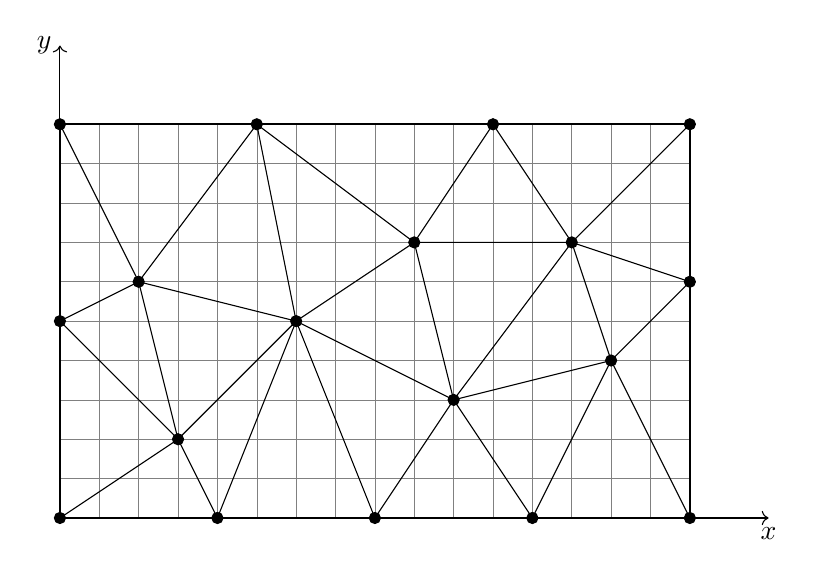
\begin{tikzpicture}
%\draw[fill=gray!8,gray!8](0,0) rectangle (10,7);
\draw[step=0.5cm,gray,very thin] (1,1) grid (9,6); %background grid
\draw[thick] (1,1) -- (9,1) -- (9,6) -- (1,6) -- cycle;  

\draw[thin,->] (1,1) -- (10,1) ; %horizontal axis
\draw[thin,->] (1,1) -- (1,7) ; %horizontal axis
\node[] at (10,0.8){$x$};
\node[] at (0.8,7){$y$};

\draw[] (1,1) -- (2.5,2) -- (4,3.5) -- (5.5,4.5) -- (6.5,6);  %1 6 11 13 14
\draw[] (3,1) -- (4,3.5) -- (6,2.5) -- (7.5,4.5) -- (9,6) ;  %2 11 12 15 16
\draw[] (3,1) -- (2.5,2) -- (1,3.5) -- (2,4) -- (1,6) ;  %2 6 7 8 9
\draw[] (5,1) -- (6,2.5) -- (7,1) -- (8,3) -- (9,4) -- (7.5,4.5) -- (6.5,6) ;  %3 12 4 18 17 15 14
\draw[] (3.5,6) -- (2,4) -- (4,3.5) -- (5,1) ;  %10 8 11 3
\draw[] (2.5,2) -- (2,4) ; %6 8
\draw[] (4,3.5) -- (3.5,6) -- (5.5,4.5) -- (7.5,4.5) ;  %11 10 13 15
\draw[] (9,1) -- (8,3) -- (6,2.5) -- (5.5,4.5) ;  %5 18 12 13
\draw[] (7.5,4.5) -- (8,3) ; %15 18

\draw[black,fill=black] (1,1)     circle (2pt); 
\draw[black,fill=black] (3,1)     circle (2pt); 
\draw[black,fill=black] (5,1)     circle (2pt); 
\draw[black,fill=black] (7,1)     circle (2pt); 
\draw[black,fill=black] (9,1)     circle (2pt); 
\draw[black,fill=black] (2.5,2)   circle (2pt); 
\draw[black,fill=black] (1,3.5)   circle (2pt); 
\draw[black,fill=black] (2,4)     circle (2pt); 
\draw[black,fill=black] (1,6)     circle (2pt); 
\draw[black,fill=black] (3.5,6)   circle (2pt); 
\draw[black,fill=black] (4,3.5)   circle (2pt); 
\draw[black,fill=black] (6,2.5)   circle (2pt); 
\draw[black,fill=black] (5.5,4.5) circle (2pt); 
\draw[black,fill=black] (6.5,6)   circle (2pt); 
\draw[black,fill=black] (7.5,4.5) circle (2pt); 
\draw[black,fill=black] (9,6)     circle (2pt); 
\draw[black,fill=black] (9,4)     circle (2pt); 
\draw[black,fill=black] (8,3)     circle (2pt); 

\end{tikzpicture}\\
\end{center}
         
We can first label the nodes:

\begin{center}
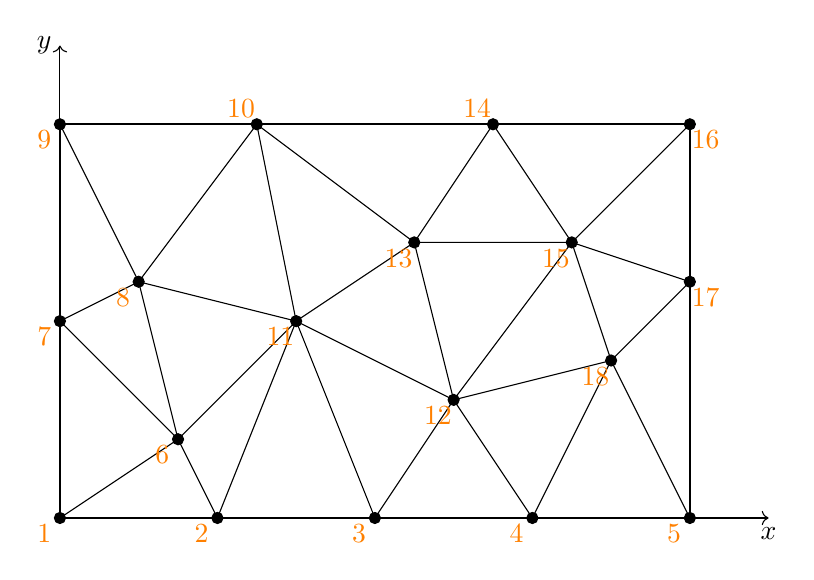
\begin{tikzpicture}
%\draw[fill=gray!5,gray!5](0,0) rectangle (10,7);
%\draw[step=0.5cm,gray,very thin] (1,1) grid (9,6); %background grid
\draw[thick] (1,1) -- (9,1) -- (9,6) -- (1,6) -- cycle;  

\draw[thin,->] (1,1) -- (10,1) ; %horizontal axis
\draw[thin,->] (1,1) -- (1,7) ; %horizontal axis
\node[] at (10,0.8){$x$};
\node[] at (0.8,7){$y$};


\draw[] (1,1) -- (2.5,2) -- (4,3.5) -- (5.5,4.5) -- (6.5,6);  %1 6 11 13 14
\draw[] (3,1) -- (4,3.5) -- (6,2.5) -- (7.5,4.5) -- (9,6) ;  %2 11 12 15 16
\draw[] (3,1) -- (2.5,2) -- (1,3.5) -- (2,4) -- (1,6) ;  %2 6 7 8 9
\draw[] (5,1) -- (6,2.5) -- (7,1) -- (8,3) -- (9,4) -- (7.5,4.5) -- (6.5,6) ;  %3 12 4 18 17 15 14
\draw[] (3.5,6) -- (2,4) -- (4,3.5) -- (5,1) ;  %10 8 11 3
\draw[] (2.5,2) -- (2,4) ; %6 8
\draw[] (4,3.5) -- (3.5,6) -- (5.5,4.5) -- (7.5,4.5) ;  %11 10 13 15
\draw[] (9,1) -- (8,3) -- (6,2.5) -- (5.5,4.5) ;  %5 18 12 13
\draw[] (7.5,4.5) -- (8,3) ; %15 18

\draw[black,fill=black] (1,1)     circle (2pt); \node[] at (0.8,0.8){\color{orange} 1}; %1
\draw[black,fill=black] (3,1)     circle (2pt); \node[] at (2.8,0.8){\color{orange} 2}; %2
\draw[black,fill=black] (5,1)     circle (2pt); \node[] at (4.8,0.8){\color{orange} 3}; %3
\draw[black,fill=black] (7,1)     circle (2pt); \node[] at (6.8,0.8){\color{orange} 4}; %4
\draw[black,fill=black] (9,1)     circle (2pt); \node[] at (8.8,0.8){\color{orange} 5}; %5
\draw[black,fill=black] (2.5,2)   circle (2pt); \node[] at (2.3,1.8){\color{orange} 6}; %6
\draw[black,fill=black] (1,3.5)   circle (2pt); \node[] at (0.8,3.3){\color{orange} 7}; %7
\draw[black,fill=black] (2,4)     circle (2pt); \node[] at (1.8,3.8){\color{orange} 8}; %8
\draw[black,fill=black] (1,6)     circle (2pt); \node[] at (0.8,5.8){\color{orange} 9}; %9
\draw[black,fill=black] (3.5,6)   circle (2pt); \node[] at (3.3,6.2){\color{orange} 10};%10
\draw[black,fill=black] (4,3.5)   circle (2pt); \node[] at (3.8,3.3){\color{orange} 11};%11
\draw[black,fill=black] (6,2.5)   circle (2pt); \node[] at (5.8,2.3){\color{orange} 12};%12
\draw[black,fill=black] (5.5,4.5) circle (2pt); \node[] at (5.3,4.3){\color{orange} 13};%13
\draw[black,fill=black] (6.5,6)   circle (2pt); \node[] at (6.3,6.2){\color{orange} 14};%14
\draw[black,fill=black] (7.5,4.5) circle (2pt); \node[] at (7.3,4.3){\color{orange} 15};%15
\draw[black,fill=black] (9,6)     circle (2pt); \node[] at (9.2,5.8){\color{orange} 16};%16
\draw[black,fill=black] (9,4)     circle (2pt); \node[] at (9.2,3.8){\color{orange} 17};%17
\draw[black,fill=black] (8,3)     circle (2pt); \node[] at (7.8,2.8){\color{orange} 18};%18
\end{tikzpicture}\\
\end{center}

and then label the elements:

\begin{center}
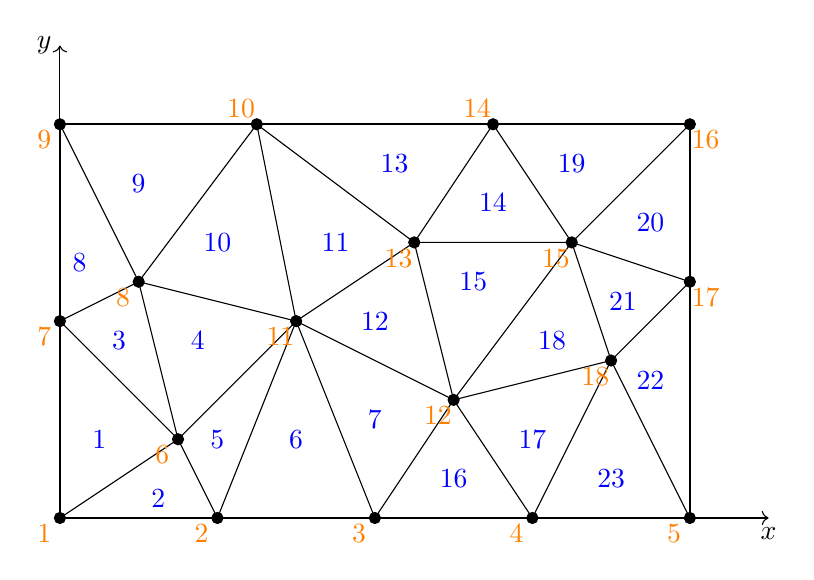
\begin{tikzpicture}
%\draw[fill=gray!5,gray!5](0,0) rectangle (10,7);
%\draw[step=0.5cm,gray,very thin] (1,1) grid (9,6); %background grid
\draw[thick] (1,1) -- (9,1) -- (9,6) -- (1,6) -- cycle;  

\draw[thin,->] (1,1) -- (10,1) ; %horizontal axis
\draw[thin,->] (1,1) -- (1,7) ; %horizontal axis
\node[] at (10,0.8){$x$};
\node[] at (0.8,7){$y$};


\draw[] (1,1) -- (2.5,2) -- (4,3.5) -- (5.5,4.5) -- (6.5,6);  %1 6 11 13 14
\draw[] (3,1) -- (4,3.5) -- (6,2.5) -- (7.5,4.5) -- (9,6) ;  %2 11 12 15 16
\draw[] (3,1) -- (2.5,2) -- (1,3.5) -- (2,4) -- (1,6) ;  %2 6 7 8 9
\draw[] (5,1) -- (6,2.5) -- (7,1) -- (8,3) -- (9,4) -- (7.5,4.5) -- (6.5,6) ;  %3 12 4 18 17 15 14
\draw[] (3.5,6) -- (2,4) -- (4,3.5) -- (5,1) ;  %10 8 11 3
\draw[] (2.5,2) -- (2,4) ; %6 8
\draw[] (4,3.5) -- (3.5,6) -- (5.5,4.5) -- (7.5,4.5) ;  %11 10 13 15
\draw[] (9,1) -- (8,3) -- (6,2.5) -- (5.5,4.5) ;  %5 18 12 13
\draw[] (7.5,4.5) -- (8,3) ; %15 18

\draw[black,fill=black] (1,1)     circle (2pt); \node[] at (0.8,0.8){\color{orange} 1}; %1
\draw[black,fill=black] (3,1)     circle (2pt); \node[] at (2.8,0.8){\color{orange} 2}; %2
\draw[black,fill=black] (5,1)     circle (2pt); \node[] at (4.8,0.8){\color{orange} 3}; %3
\draw[black,fill=black] (7,1)     circle (2pt); \node[] at (6.8,0.8){\color{orange} 4}; %4
\draw[black,fill=black] (9,1)     circle (2pt); \node[] at (8.8,0.8){\color{orange} 5}; %5
\draw[black,fill=black] (2.5,2)   circle (2pt); \node[] at (2.3,1.8){\color{orange} 6}; %6
\draw[black,fill=black] (1,3.5)   circle (2pt); \node[] at (0.8,3.3){\color{orange} 7}; %7
\draw[black,fill=black] (2,4)     circle (2pt); \node[] at (1.8,3.8){\color{orange} 8}; %8
\draw[black,fill=black] (1,6)     circle (2pt); \node[] at (0.8,5.8){\color{orange} 9}; %9
\draw[black,fill=black] (3.5,6)   circle (2pt); \node[] at (3.3,6.2){\color{orange} 10};%10
\draw[black,fill=black] (4,3.5)   circle (2pt); \node[] at (3.8,3.3){\color{orange} 11};%11
\draw[black,fill=black] (6,2.5)   circle (2pt); \node[] at (5.8,2.3){\color{orange} 12};%12
\draw[black,fill=black] (5.5,4.5) circle (2pt); \node[] at (5.3,4.3){\color{orange} 13};%13
\draw[black,fill=black] (6.5,6)   circle (2pt); \node[] at (6.3,6.2){\color{orange} 14};%14
\draw[black,fill=black] (7.5,4.5) circle (2pt); \node[] at (7.3,4.3){\color{orange} 15};%15
\draw[black,fill=black] (9,6)     circle (2pt); \node[] at (9.2,5.8){\color{orange} 16};%16
\draw[black,fill=black] (9,4)     circle (2pt); \node[] at (9.2,3.8){\color{orange} 17};%17
\draw[black,fill=black] (8,3)     circle (2pt); \node[] at (7.8,2.8){\color{orange} 18};%18


\node[] at (1.5,2) {\color{blue}1};
\node[] at (2.25,1.25) {\color{blue}2};
\node[] at (1.75,3.25) {\color{blue}3};
\node[] at (2.75,3.25) {\color{blue}4};
\node[] at (3,2) {\color{blue}5};
\node[] at (4,2) {\color{blue}6};
\node[] at (5,2.25) {\color{blue}7};
\node[] at (1.25,4.25) {\color{blue}8};
\node[] at (2,5.25) {\color{blue}9};
\node[] at (3,4.5) {\color{blue}10};
\node[] at (4.5,4.5) {\color{blue}11};
\node[] at (5,3.5) {\color{blue}12};
\node[] at (5.25,5.5) {\color{blue}13};
\node[] at (6.5,5) {\color{blue}14};
\node[] at (6.25,4) {\color{blue}15};
\node[] at (6,1.5) {\color{blue}16};
\node[] at (7,2) {\color{blue}17};
\node[] at (7.25,3.25) {\color{blue}18};
\node[] at (7.5,5.5) {\color{blue}19};
\node[] at (8.5,4.75) {\color{blue}20};
\node[] at (8.15,3.75) {\color{blue}21};
\node[] at (8.5,2.75) {\color{blue}22};
\node[] at (8,1.5) {\color{blue}23};


\end{tikzpicture}\\
\end{center}

We can finally build the connectivity array by hand:

\noindent
icon(1,{\color{blue}1})={\color{orange}1}\\
icon(2,{\color{blue}1})={\color{orange}6}\\
icon(3,{\color{blue}1})={\color{orange}7}\\
icon(1,{\color{blue}2})={\color{orange}1}\\
icon(2,{\color{blue}2})={\color{orange}2}\\
icon(3,{\color{blue}2})={\color{orange}6}\\
icon(1,{\color{blue}3})={\color{orange}7}\\
icon(2,{\color{blue}3})={\color{orange}6}\\
icon(3,{\color{blue}3})={\color{orange}8}\\
...\\
icon(1,{\color{blue}12})={\color{orange}11}\\
icon(2,{\color{blue}12})={\color{orange}12}\\
icon(3,{\color{blue}12})={\color{orange}13}\\
...\\
icon(1,{\color{blue}19})={\color{orange}14}\\
icon(2,{\color{blue}19})={\color{orange}15}\\
icon(3,{\color{blue}19})={\color{orange}16}\\


The labelling of nodes and elements above is done by a human so it starts at 1. When 
implementing this in python, you know what to do ...


%-----------------------------------------------
\subsection{How to visualise data on a triangular mesh with Paraview}

If arrays {\tt x,y} contain the coordinates of the nodes, your connectivity array is called {\tt icon},
and your mesh consistes of {\tt nel} elements and comprises {\tt nnp} nodes, you can use the following code
to generate a vtu file to be opened with Paraview. You also need a temperature array {\tt T}.

\begin{center}
Code at \url{https://raw.githubusercontent.com/cedrict/fieldstone/master/images/compgeo/mesh_visu.py}
\end{center}

\lstinputlisting[language=python]{images/compgeo/mesh_visu.py}
 %%%%%%%%%%%%%%%%%%%%%%%%%%%
\chapter{Using prisms in forward gravity modelling \label{app:prisms}} 
{\sl This appendix was written by Sverre Hassing as part of his Bachelor thesis.} \index{contributors}{S. Hassing}
Although the final formula are definitely correct, the derivations below may still contain a typo. 

\vspace{.4cm}

The derivations for prisms have been published in the early 50's \cite{made51}. 
However, to the best of our knowledge the full derivation has not been carried out in English in full detail. 
The derivations are based on those of Mader (1951) \cite{made51} and of Nagy \etal (2000) \cite{napb00,napb02}. 
Mader provided the derivations in some detail, while Nagy \etal interpreted the results in a more modern style. 


%----------------------------
\subsection{Basic formulas}

The derivations for prisms are a lot more complicated than that for the point masses. 
We start with the following two integral equations which are integral part of the derivations:

\begin{eqnarray}
\int \frac{x^2 dx}{x^2 + z^2} &=& x - z  \arctan{\frac{x}{z}} \label{eq:basic1} \\
\int \frac{dx}{\sqrt{x^2+y^2+z^2}} &=& \ln{\left( x + \sqrt{x^2+y^2+z^2} \right)} \label{eq:basic2}
\end{eqnarray}
Another equation that will come back multiple times is of the form:
\begin{equation}
\int \frac{du}{(v^2+w^2)\sqrt{u^2+v^2+w^2}}
\end{equation}
This can be solved with a trigonometric substitution, where $u = \sqrt{v^2+w^2} \tan{\phi}$. This means that $du = \frac{\sqrt{v^2+w^2}}{cos^2{\phi}} d\phi$.
\begin{eqnarray}
\int \frac{du}{(v^2+w^2)\sqrt{u^2+v^2+w^2}} 
&=& 
\int \frac{\sqrt{v^2+w^2}}{cos^2{\phi}} 
\frac{1}{(v^2+w^2)\tan^2{\phi}+v^2} 
\frac{d\phi}{\sqrt{v^2+w^2+(v^2+w^2)\tan^2{\phi})}} \nonumber\\
&=& 
\int \frac{\sqrt{v^2+w^2}}{cos{\phi}^2} 
\frac{1}{v^2(\tan^2{\phi}+1) + w^2 \tan^2{\phi}} 
\frac{d\phi}{\sqrt{(v^2+w^2)(\tan^2{\phi}+1)}} \nonumber\\
&=&
\int \frac{\sqrt{v^2+w^2}}{cos{\phi}^2} 
\frac{1}{\frac{v^2+w^2 \sin^2{\phi}}{cos^2{\phi}}} 
\frac{d\phi}{\frac{\sqrt{v^2+w^2}}{cos{\phi}}} \nonumber\\
&=& 
\int \frac{\cos{\phi} d\phi}{v^2+w^2\sin^2{\phi}}
\end{eqnarray}
A second substitution is needed where $t = \frac{w}{v}\sin{\phi}$ and $dt = \frac{v}{w} \cos{\phi} d\phi$:
\begin{eqnarray}
\int \frac{\cos{\phi} d\phi}{v^2+w^2\sin^2{\phi}} 
&=& \int \frac{v dt}{w (v^2+v^2t^2)} \nonumber\\
&=& \frac{1}{vw} \int \frac{dt}{1+t^2} \nonumber\\
&=& \frac{1}{vw} \arctan{t} \nonumber\\
&=& \frac{1}{vw} \arctan{\frac{w \sin{\phi}}{v}} \label{eq:prismbe1}
\end{eqnarray}
Now the $\sin{\phi}$ needs to be converted back to $u,v,w$. If it is known that $\tan{\phi} = \frac{u}{\sqrt{v^2+w^2}}$, then it follows that $\sin{\phi}=\frac{u}{\sqrt{u^2+v^2+w^2}}$.
Eq.\eqref{eq:prismbe1} then becomes
\begin{equation}
{\frac{1}{vw} \arctan \frac{w \sin{\phi}}{v}} = \frac{1}{vw} \arctan{\frac{u w}{v \sqrt{u^2+v^2+w^2}}}
\end{equation}
and finally 
\begin{equation}
\boxed{
\int \frac{du}{(v^2+w^2)\sqrt{u^2+v^2+w^2}} = \frac{1}{vw} \arctan{\frac{u w}{v \sqrt{u^2+v^2+w^2}}} \label{eq:basic3}
}
\end{equation}

\subsection{The gravitational potential}

Each prism is assumed to have constant density $\rho$. The gravitational potential is integrated over the whole volume of the prism:
\begin{equation}
U(P) =  -{\cal G}  \rho \underbrace{\int_{x_1}^{x_2} \int_{y_1}^{y_2} \int_{z_1}^{z_2} \frac{dx dy dz}{\sqrt{x^2+y^2+z^2}}}_{I} \label{eq:der_U_1}
\end{equation}

In what follows we work out the exact form for the triple integral term. Elementary Eq.~\eqref{eq:basic2} can be applied to the integral for $dx$ 
in Eq.~\eqref{eq:der_U_1}.
\begin{eqnarray}
I
&=& \iiint \frac{dx dy dz}{\sqrt{x^2+y^2+z^2}}  \nn\\
&=& \iint \left(\int \frac{dx}{\sqrt{x^2+y^2+z^2}} \right) dydz \nonumber\\
&=& \iint \ln{\left( x+\sqrt{x^2+y^2+z^2} \right)} dy dz
\end{eqnarray}
We further proceed with the integration with respect to $y$. We define
\[
\begin{array}{c|c}
  f = \int \ln{\left( x+\sqrt{x^2+y^2+z^2} \right)} dz 
  & g' = dy \\ 
  \hline
  f' = \frac{y}{\left( x+\sqrt{x^2+y^2+z^2} \right) \sqrt{x^2+y^2+z^2}} 
  & g=y
 \end{array}
\]
and using $\int f g'  = f g - \int f g'$ we have 
\begin{equation}
I= 
\underbrace{y \int \ln{ \left( x + \sqrt{x^2+y^2+z^2} \right) } dz}_{A} 
\underbrace{- \iint  \frac{y^2 dz}{\left( x+\sqrt{x^2+y^2+z^2}\right) \sqrt{x^2+y^2+z^2}} dy}_{B} 
\end{equation}

The calculation of $I$ is then split into two large integrals denoted
$A$ and $B$, calculated in the following subsections.
Note that we have not made use of the integral bounds yet.  

%..................................................................
\subsubsection{The calculation of $A$} \label{subsection:calc_A}

The first step in calculating $A$ is to carry out a similar partial integration as seen before. 

\[
\begin{array}{c|c}
  f=\ln{ \left( x + \sqrt{x^2+y^2+z^2} \right)} & 
  g'=dz \\ 
  \hline
  f' = \frac{\partial f}{\partial z} = \frac{z}{\left( x+\sqrt{x^2+y^2+z^2} \right) \sqrt{x^2+y^2+z^2}} 
  & g = z
 \end{array}
\]

\begin{eqnarray}
A 
&=& 
y \left(z \ln{ \left( x + \sqrt{x^2+y^2+z^2} \right)} - 
\int \frac{z^2 dz}{\left( x+\sqrt{x^2+y^2+z^2} \right) \sqrt{x^2+y^2+z^2}} \right) \nonumber\\
&=& 
\underbrace{yz \ln{ \left( x + \sqrt{x^2+y^2+z^2} \right)} }_{A_0} 
- 
\underbrace{y\int \frac{z^2 dz}{\left( x+\sqrt{x^2+y^2+z^2} \right) \sqrt{x^2+y^2+z^2}}  }_{A_1}
\end{eqnarray}

We now focus on the $A_1$ integral. 
We first multiply the numerator and denominator by $-x+\sqrt{x^2+y^2+z^2} $. The last step uses Eqs.~\eqref{eq:basic2}, \eqref{eq:basic3} and \eqref{eq:basic1} respectively for each term.
\begin{eqnarray}
A_1 
&=& \int \frac{z^2 dz}{\left( x+\sqrt{x^2+y^2+z^2} \right) \sqrt{x^2+y^2+z^2}}
\frac{-x+\sqrt{x^2+y^2+z^2}}{-x+\sqrt{x^2+y^2+z^2}} \nonumber\\
&=& \int \frac{(-x z^2 + z^2 \sqrt{x^2+y^2+z^2} )dz}{\left( x^2+y^2+z^2 - x^2 \right) \sqrt{x^2+y^2+z^2}} \label{eq:der_U_2} \nonumber\\
&=& 
\int \frac{-x z^2 dz}{\left( y^2+z^2  \right) \sqrt{x^2+y^2+z^2}}  
+ \int \frac{z^2 \sqrt{x^2+y^2+z^2} dz}{\left( y^2+z^2  \right) \sqrt{x^2+y^2+z^2}} \nonumber\\
&=& \int \frac{-x \left( z^2 + y^2 -y^2 \right) dz}{(y^2+z^2)\sqrt{x^2+y^2+z^2}} + 
\int \frac{z^2dz}{y^2+z^2} \nonumber\\
&=& \int \frac{-x dz}{\sqrt{x^2+y^2+z^2}} + 
\int \frac{x y^2 dz}{(y^2+z^2)\sqrt{x^2+y^2+z^2}} + 
\int \frac{z^2dz}{y^2+z^2} \nonumber\\
&=& -x \int \frac{ dz}{\sqrt{x^2+y^2+z^2}} + 
x y^2 \int \frac{ dz}{(y^2+z^2)\sqrt{x^2+y^2+z^2}} + 
\int \frac{z^2dz}{y^2+z^2} \nonumber\\
&=& -x \ln{ \left( z + \sqrt{x^2+y^2+z^2} \right)} + 
y \arctan{\frac{x z}{y \sqrt{x^2+y^2+z^2}}} + 
z -  y \arctan{\frac{z}{y}}
\end{eqnarray}
This can be combined to get the final expression for A:
\begin{equation}
A = 
y \left( z \ln{ \left( x + \sqrt{x^2+y^2+z^2} \right)} + 
x \ln{ \left( z + \sqrt{x^2+y^2+z^2} \right)} -  
y \arctan{\frac{x z}{y \sqrt{x^2+y^2+z^2}}} - 
z + 
y \arctan{\frac{z}{y}} \right)
\end{equation}
The last two terms can be left out because they will cancel out when computing the integration boundaries from $x_1$ to $x_2$, because these terms do not contain the variable $x$. 
Finally we arrive at the following expression for $A$:
\begin{equation}
A = 
yz \ln{\left( x + \sqrt{x^2+y^2+z^2} \right)} + 
xy \ln{\left( z + \sqrt{x^2+y^2+z^2} \right)} - 
y^2 \arctan{\frac{xz}{y\sqrt{x^2+y^2+z^2}}}
\end{equation}



%.......................................
\subsubsection{The calculation of $B$}

The inner integral can be simplified similarly to how $A_1$ was simplified in Eq.~\eqref{eq:der_U_2}, 
by multiplying both numerator and denominator with $-x+\sqrt{x^2+y^2+z^2}$. The last step uses Eqs.~\eqref{eq:basic3} and \eqref{eq:basic1}:
\begin{eqnarray}
B 
&=& 
-\int y^2 \int \frac{dz}{\left( x + \sqrt{x^2+y^2+z^2} \right) \sqrt{x^2+y^2+z^2}} 
\frac{-x + \sqrt{x^2+y^2+z^2}}{-x + \sqrt{x^2+y^2+z^2}} dy \nonumber\\
&=& - \int y^2 \int \frac{-x + \sqrt{x^2+y^2+z^2} }{\left( x^2 + y^2+z^2 -x^2 \right) \sqrt{x^2+y^2+z^2}}dz dy \nonumber\\
&=& - \int y^2 \left( 
- \int \frac{x dz}{(y^2+z^2)\sqrt{x^2+y^2+z^2}} +
\int \frac{dz}{y^2+z^2} 
\right) dy \nonumber\\
&=& - \int y^2 \left( -\frac{1}{y} \arctan{\frac{xz}{y\sqrt{x^2+y^2+z^2}}} + \frac{1}{y} \arctan{\frac{z}{y}}\right) dy \nn\\
&=& \int y \arctan{\frac{xz}{y\sqrt{x^2+y^2+z^2}}} dy
\end{eqnarray}
Again the second term can be left out, because it does not contain the variable $x$. The next step is to apply a partial integration to $B$.  

\[
\begin{array}{c|c}
  f=\arctan{\frac{xz}{y\sqrt{x^2+y^2+z^2}}} & g'=y \\ 
  \hline
  f' = -xz \frac{\frac{1}{y^2 \sqrt{x^2+y^2+z^2}}+\frac{1}{(x^2+y^2+z^2)^\frac{3}{2}}}{\frac{x^2z^2}{y^2(x^2+y^2+z^2)}+1} & g = \frac{y^2}{2}
 \end{array}
\]

\begin{equation}
B = 
\frac{y^2}{2} \arctan{\frac{xz}{y\sqrt{x^2+y^2+z^2}}} +
\underbrace{
\frac{xz}{2} \int y^2 \frac{\frac{1}{y^2\sqrt{x^2+y^2+z^2}}+\frac{1}{(x^2+y^2+z^2)^\frac{3}{2}}}{\frac{x^2z^2}{y^2(x^2+y^2+z^2)}+1}}_{B_1}
\end{equation}

Let us finish by calculating the integral $B_1$:

\begin{eqnarray}
B_1 
&=& 
\frac{xz}{2} \int y^2 
\frac{\frac{1}{y^2\sqrt{x^2+y^2+z^2}}+\frac{1}{(x^2+y^2+z^2)^{3/2}}}{\frac{x^2z^2}{y^2(x^2+y^2+z^2)}+1} 
dy \nonumber\\
&=& 
\frac{xz}{2} \int y^2 
\frac{\frac{x^2+y^2+z^2}{y^2(x^2+y^2+z^2)^{3/2}}+\frac{y^2}{y^2(x^2+y^2+z^2)^{3/2}}}{\frac{x^2z^2+y^2(x^2+y^2+z^2)}{y^2(x^2+y^2+z^2)}} 
dy \nonumber\\
&=& 
\frac{xz}{2} \int y^2 
\frac{\frac{x^2+2y^2+z^2}{y^2(x^2+y^2+z^2)^{3/2}}}{\frac{x^2z^2+y^2(x^2+y^2+z^2)}{y^2(x^2+y^2+z^2)}} 
dy \nonumber\\
&=& 
\frac{xz}{2} \int y^2 
\frac{x^2+2y^2+z^2}{\sqrt{x^2+y^2+z^2}(x^2z^2+y^2(x^2+y^2+z^2))} 
dy \nonumber\\
&=& 
\frac{xz}{2} 
\int y^2 \frac{x^2+2y^2+z^2}{\sqrt{x^2+y^2+z^2}(x^2+y^2)(z^2+y^2)} 
dy \nonumber\\
&=& 
\frac{xz}{2} 
\left( 
\int \frac{2dy}{\sqrt{x^2+y^2+z^2}} + 
\int \frac{-(x^2+z^2)y^2-2x^2z^2}{(x^2+y^2)(y^2+z^2)\sqrt{x^2+y^2+z^2}} 
dy \right) \nonumber\\
&=& 
xz \ln{\left( y + \sqrt{x^2+y^2+z^2} \right)} - 
\frac{xz}{2} 
\int \frac{(x^2+z^2)y^2+2x^2z^2}{(x^2+y^2)(y^2+z^2)\sqrt{x^2+y^2+z^2}} 
dy \nonumber\\
&=& 
xz \ln{\left( y + \sqrt{x^2+y^2+z^2} \right)} - 
\frac{xz}{2} \int \frac{x^2y^2+y^2z^2+2x^2z^2}{(x^2+y^2)(y^2+z^2)\sqrt{x^2+y^2+z^2}} 
dy \nonumber\\
&=& 
xz \ln{\left( y + \sqrt{x^2+y^2+z^2} \right)} - 
\frac{xz}{2} \int \frac{x^2(y^2+z^2)+z^2(x^2+y^2)}{(x^2+y^2)(y^2+z^2)\sqrt{x^2+y^2+z^2}} 
dy \nonumber\\
&=& 
xz \ln{\left( y + \sqrt{x^2+y^2+z^2} \right)} - 
\frac{xz}{2} \int \frac{x^2}{(x^2+y^2)\sqrt{x^2+y^2+z^2}} dy - 
\frac{xz}{2} \int \frac{z^2}{(y^2+z^2)\sqrt{x^2+y^2+z^2}} 
dy \nonumber\\
&=& 
xz \ln{\left( y + \sqrt{x^2+y^2+z^2} \right)} - 
\frac{xz}{2} \frac{x^2\arctan{\frac{yz}{x\sqrt{x^2+y^2+z^2}}}}{xz} - 
\frac{xz}{2} \frac{z^2\arctan{\frac{xy}{z\sqrt{x^2+y^2+z^2}}}}{xz} 
\nonumber\\
&=& 
xz \ln{\left( y + \sqrt{x^2+y^2+z^2} \right)} - 
\frac{x^2}{2} \arctan{\frac{yz}{x\sqrt{x^2+y^2+z^2}}} - 
\frac{z^2}{2} \arctan{\frac{xy}{z\sqrt{x^2+y^2+z^2}}}
\end{eqnarray}
This can be combined to get the full expression for $B$:
\[
B = 
xz \ln{\left( \sqrt{x^2+y^2+z^2}+y \right)} - 
\frac{x^2}{2} \arctan{\frac{zy}{x\sqrt{x^2+y^2+z^2}}} + 
\frac{y^2}{2} \arctan{\frac{xz}{y\sqrt{x^2+y^2+z^2}}} - 
\frac{z^2}{2} \arctan{\frac{xy}{x\sqrt{z^2+y^2+z^2}}}
\]

%..............................................
\subsubsection{Combining $A$ and $B$}
Now A and B can be combined to get the expression of $I$ 

\begin{eqnarray}
I&=& A + B \nonumber\\
&=& yz \ln{\left( x + \sqrt{x^2+y^2+z^2} \right)} + 
xy \ln{\left( z + \sqrt{x^2+y^2+z^2} \right)} - 
y^2 \arctan{\frac{xz}{y\sqrt{x^2+y^2+z^2}}} \nonumber\\ 
&+& 
xz \ln{\left( \sqrt{x^2+y^2+z^2}+y \right)} - 
\frac{x^2}{2} \arctan{\frac{zy}{x\sqrt{x^2+y^2+z^2}}} + 
\frac{y^2}{2} \arctan{\frac{xz}{y\sqrt{x^2+y^2+z^2}}} - 
\frac{z^2}{2} \arctan{\frac{xy}{x\sqrt{z^2+y^2+z^2}}} \nonumber\\
&=&
yz \ln{\left( x + \sqrt{x^2+y^2+z^2} \right)} + 
xy \ln{\left( z + \sqrt{x^2+y^2+z^2} \right)} + 
xz \ln{\left( y+\sqrt{x^2+y^2+z^2} \right)} \nonumber\\ 
&-& 
\frac{x^2}{2} \arctan{\frac{zy}{x\sqrt{x^2+y^2+z^2}}} - 
\frac{y^2}{2} \arctan{\frac{xz}{y\sqrt{x^2+y^2+z^2}}} - 
\frac{z^2}{2} \arctan{\frac{xy}{x\sqrt{z^2+y^2+z^2}}} 
\end{eqnarray}

The boundaries for the volume from Eq.~\eqref{eq:def_points} need to be applied to the result of the integration. 
The boundary conditions are computed by plugging the upper value into the equation and subtracting the equation with the lower 
value plugged in. When the upper and lower values are respectively $x_2$ and $x_1$ for some function $f(x)$, this is $f(x_2) - f(x_1)$. 
This can be represented more efficiently with a summation over the subscript. Something needs to be added to still keep the subtraction in there. 
This can be done by adding a factor of $-1^i$, where i is the summation index. This will be positive when $i$ is even and negative when $i$ is odd. 
The new way of showing the result would be $\displaystyle\sum_{i=1}^{2} -1^i f(x_i)$. This is especially useful when there are three different 
integration boundaries to resolve. $r$ will be used instead of $\sqrt{x^2+y^2+z^2}$. 

\begin{eqnarray}
I
&=& \left| \left| \left| 
yz \ln{\left( x + r \right)} + 
xy \ln{\left( z + r \right)} + 
xz \ln{\left( y + r \right)} - 
\frac{x^2}{2} \arctan{\frac{zy}{xr}} - 
\frac{y^2}{2} \arctan{\frac{xz}{yr}} - 
\frac{z^2}{2} \arctan{\frac{xy}{xr}} 
\right|_{x_1}^{x_2} \right|_{y_1}^{y_2} \right|_{z_1}^{z_2} 
\nonumber\\
&=& \sum_{i=1}^{2} \sum_{j=1}^{2} \sum_{k=1}^{2} (-1)^{i+j+k} 
\Bigg(
y_j z_k \ln{\left( x_i + r_{ijk} \right)} + 
x_i y_j \ln{\left( z_k + r_{ijk} \right)} + 
x_i z_k \ln{\left( y_j+r_{ijk} \right)}  \nonumber\\
&& \qquad\qquad\qquad\qquad\qquad \left. - 
\frac{x_i^2}{2} \arctan{\frac{z_k y_j}{x_i r_{ijk}}} - 
\frac{y_j^2}{2} \arctan{\frac{x_i z_k}{y_j r_{ijk}}} - 
\frac{z_k ^2}{2} \arctan{\frac{x_i y_j}{x_i r_{ijk}}} 
\right)
\end{eqnarray} 

\todo[inline]{There is probably a mistake in eq above and below, last term, most likely should contain zk in denominator?}

Finally,
\begin{mdframed}[backgroundcolor=blue!5]
\begin{eqnarray}
U(\vec{r}) &=& {\cal G}  \rho 
\sum_{i=1}^{2} \sum_{j=1}^{2} \sum_{k=1}^{2} (-1)^{i+j+k} \Bigg( 
y_j z_k \ln{\left( x_i + r_{ijk} \right)} + 
x_i y_j \ln{\left( z_k + r_{ijk} \right)} + 
x_i z_k \ln{\left( y_j+r_{ijk} \right)}   \nn\\ 
&&  \qquad \qquad - 
\frac{x_i^2}{2} \arctan{\frac{z_k y_j}{x_i r_{ijk}}} - 
\frac{y_j^2}{2} \arctan{\frac{x_i z_k}{y_j r_{ijk}}} - 
\frac{z_k^2}{2} \arctan{\frac{x_i y_j}{x_i r_{ijk}}} 
\Bigg) 
\end{eqnarray}
\end{mdframed}








%------------------------------------------
\subsection{The gravity vector $\vec{g}$}

In 3D Cartesian coordinates the gravity vector is expressed as
\begin{equation}
\vec{g} = -\vec\nabla U  = 
\left( 
\begin{array}{c} 
-\frac{\partial U}{\partial x} \\ \\
-\frac{\partial U}{\partial y} \\ \\
-\frac{\partial U}{\partial z} 
\end{array} \right)
\end{equation}
The easiest way to calculate this is by including the partial derivatives in the original integral \eqref{eq:der_U_1}.
\begin{eqnarray}
I_x(\vec{r}) 
&=& \iiint \frac{\partial}{\partial x} \frac{dx dy dz}{\sqrt{x^2+y^2+z^2}} \nonumber\\
&=& -\iiint \frac{x dx dy dz}{(\sqrt{x^2+y^2+z^2})^3} \nonumber\\
&=& \iint \frac{dy dz}{\sqrt{x^2+y^2+z^2}}
\end{eqnarray}

The integral \eqref{eq:basic2} can be used, followed by the calculation of $A$ as seen in Section~\ref{subsection:calc_A} 
without the multiplication with $y$:
\begin{eqnarray}
I_x(\vec{r})
&=& \int \ln{\left( x + \sqrt{x^2+y^2+z^2} \right)} dz \nonumber\\
&=& 
z \ln{\left( y + \sqrt{x^2+y^2+z^2} \right)} + 
y \ln{\left( z + \sqrt{x^2+y^2+z^2} \right)} - 
x \arctan{\frac{yz}{x \sqrt{x^2+y^2+z^2}}}
\end{eqnarray}
The integration boundaries can be applied. Multiplication with ${\cal G}$ and $\rho$ is the final step in deriving the element of 
the gravity vector component ($g_x$). 

\begin{eqnarray}
g_x = 
{\cal G}  \rho \sum_{i,j,k=1}^{2} (-1)^{i+j+k}  \left( 
z_k \ln{\left( y_j + \sqrt{x_i^2+y_j^2+z_k^2} \right)} + 
y_j \ln{\left( z_j + \sqrt{x_i^2+y_j^2+z_k^2} \right)} - 
x_i \arctan{\frac{y_j z_k}{x_i \sqrt{x_i^2+y_j^2+z_k^2}}} \right) \nn
\end{eqnarray}

The same can be done for the $y-$ and $z-$components and in the end we obtain
\begin{mdframed}[backgroundcolor=blue!5]
\begin{eqnarray}
g_x &=& {\cal G}  \rho \displaystyle\sum_{i=1}^{2} \displaystyle\sum_{j=1}^{2} \displaystyle\sum_{k=1}^{2} (-1)^{i+j+k} 
\left( 
z_k \ln{\left( y_j + r_{ijk} \right)} + 
y_j \ln{\left( z_j + r_{ijk} \right)} - 
x_i \arctan{\frac{y_j z_k}{x_i r_{ijk}}} 
\right) \nonumber\\
g_y &=& 
{\cal G}  \rho \displaystyle\sum_{i=1}^{2} \displaystyle\sum_{j=1}^{2} \displaystyle\sum_{k=1}^{2} (-1)^{i+j+k} 
\left( 
z_k \ln{\left( x_i + r_{ijk} \right)} + 
x_i \ln{\left( z_j + r_{ijk} \right)} - 
y_j \arctan{\frac{x_i z_k}{y_j r_{ijk}}} 
\right) \nonumber\\
g_z &=& 
{\cal G}  \rho \displaystyle\sum_{i=1}^{2} \displaystyle\sum_{j=1}^{2} \displaystyle\sum_{k=1}^{2} (-1)^{i+j+k} 
\left( 
x_i \ln{\left( y_j + r_{ijk} \right)} + 
y_j \ln{\left( x_i + r_{ijk} \right)} - 
z_k \arctan{\frac{x_i y_j}{z_k r_{ijk}}} 
\right) \nonumber
\end{eqnarray}
\end{mdframed}

These equations can be found in various other papers such as Eq.~(6) in Heck and Seitz, 2007 \cite{hese07}, Eqs.~(8,11,12) in Nagy \etal, 2000 \cite{napb00} 
(note that there is a mistake there that is later fixed in \cite{napb02}), 
appendix A in Couder-Castaneda \etal., 2015 \cite{cooo15} 
and the derivation between (14) and (15) in Mader, 1951 \cite{made51}.

%-------------------------------------------------------
\subsection{The gravity gradient tensor} % (${\bm T}$)}

The different elements of the gravity gradient tensor can be determined by partially differentiating each component of the 
gravity vector with respect to each space coordinate. As will be shown later, ${\bm T}$ should be a symmetric matrix and its trace should equal zero.

%...............................
\subsubsection{The diagonal terms}

\begin{eqnarray}
T_{xx} 
&=& \frac{\partial}{\partial x} g_x 
= -\frac{\partial^2}{\partial x^2} U(\vec{r}) 
= {\cal G} \rho \frac{\partial^2}{\partial x^2} \left( -I(\vec{r}) \right)
\end{eqnarray}

\begin{eqnarray}
I_{xx}(\vec{r}) 
&=& \iiint \frac{\partial^2}{\partial x^2} \frac{dx dy dz}{\sqrt{x^2+y^2+z^2}} \nonumber\\
&=& \iint \frac{\partial}{\partial x} \frac{dy dz}{\sqrt{x^2+y^2+z^2}} \nonumber\\
&=& - \iint \frac{x dy dz}{\sqrt{x^2+y^2+z^2}^3}
\end{eqnarray}

A trigonometric substitution is applied to solve this integral. 
This uses $y = \sqrt{x^2+z^2}\tan{\phi}$ and $dy = \frac{\sqrt{x^2+y^2}}{\cos^2{\phi}}d\phi$.

\begin{eqnarray}
I_{xx} 
&=& -x \iint \frac{\sqrt{x^2+y^2}}{\cos^2{\phi}} 
\frac{d\phi dz}{\sqrt{(x^2+z^2)\tan^2{\phi}+x^2+z^2}^3} \nonumber\\
&=& -x \iint \frac{\sqrt{x^2+y^2}}{\cos^2{\phi}} 
\frac{d\phi dz}{\sqrt{(x^2+z^2)(\tan^2{\phi}+1)}^3} \nonumber\\
&=& -x \iint \frac{\sqrt{x^2+y^2}}{\cos^2{\phi}} 
\frac{d\phi dz}{\left( \frac{\sqrt{(x^2+z^2)}}{\cos{\phi}} \right)^3} \nonumber\\
&=& -x \int \frac{1}{x^2+z^2} \int \cos{\phi} \; d\phi dz \nonumber\\
&=& -x \int \frac{1}{x^2+z^2} \sin{\phi} dz
\end{eqnarray}
Now the substitution needs to be undone. If $\tan{\phi} = \frac{y}{\sqrt{x^2+z^2}}$, then $\sin{\phi} = \frac{y}{\sqrt{x^2+y^2+z^2}}$ and then
\begin{equation}
I_{xx} = -xy \int \frac{dz}{(x^2+z^2)\sqrt{x^2+y^2+z^2}}
\end{equation}
This can be solved by applying equation \eqref{eq:basic3}.
\begin{eqnarray}
I_{xx} 
&=& -\frac{xy}{xy} \arctan{\frac{yz}{x\sqrt{x^2+y^2+z^2}}} \nonumber\\
&=& -\arctan{\frac{y z}{x \sqrt{x^2+y^2+z^2}}} \nn
\end{eqnarray}

The tensor element $T_{xx}$ is then formulated as follows 
(the other elements of the diagonal are found by cyclic permutation of $x$, $y$ and $z$):

\begin{mdframed}[backgroundcolor=blue!5]
\begin{eqnarray}
T_{xx} &=& {\cal G} \rho \sum_{i=1}^{2} \sum_{j=1}^{2} \sum_{k=1}^{2} (-1)^{i+j+k} 
\left( - \arctan{\frac{y_j z_k}{x_i r_{ijk}}} \right) \nonumber\\
T_{yy} &=& {\cal G} \rho \sum_{i=1}^{2} \sum_{j=1}^{2} \sum_{k=1}^{2} (-1)^{i+j+k} 
\left( - \arctan{\frac{x_i z_k}{y_j r_{ijk}}} \right) \nonumber\\
T_{zz} &=& {\cal G} \rho \sum_{i=1}^{2} \sum_{j=1}^{2} \sum_{k=1}^{2} (-1)^{i+j+k} 
\left( - \arctan{\frac{x_i y_j}{z_k r_{ijk}}} \right) \nonumber
\end{eqnarray}
\end{mdframed}

%....................................................
\subsubsection{The off-diagonal terms of the tensor}

The other elements are easier to calculate, because the partial derivatives cancel out the integrals:

\begin{eqnarray}
I_{xy} 
&=& \iiint \frac{\partial^2}{\partial x \partial y} \frac{dx dy dz}{\sqrt{x^2+y^2+z^2}} \nonumber\\
&=& \iint \frac{\partial}{\partial y} \frac{dy dz}{\sqrt{x^2+y^2+z^2}} \nonumber\\
&=& \int \frac{dz}{\sqrt{x^2+y^2+z^2}} \nonumber\\
&=& \ln{\left(z + \sqrt{x^2+y^2+z^2} \right)}
\end{eqnarray}

\begin{eqnarray}
I_{xz} 
&=& \iiint \frac{\partial^2}{\partial x \partial z} \frac{dx dy dz}{\sqrt{x^2+y^2+z^2}} \nonumber\\
&=& \iint \frac{\partial}{\partial z} \frac{dy dz}{\sqrt{x^2+y^2+z^2}} \nonumber\\
&=& \int \frac{dy}{\sqrt{x^2+y^2+z^2}} \nonumber\\
&=& \ln{\left(y + \sqrt{x^2+y^2+z^2} \right)}
\end{eqnarray}

\begin{eqnarray}
I_{yz} 
&=& \iiint \frac{\partial^2}{\partial y \partial z} \frac{dx dy dz}{\sqrt{x^2+y^2+z^2}} \nonumber\\
&=& \iint \frac{\partial}{\partial z} \frac{dx dz}{\sqrt{x^2+y^2+z^2}} \nonumber\\
&=& \int \frac{dx}{\sqrt{x^2+y^2+z^2}} \nonumber\\
&=& \ln{\left(x + \sqrt{x^2+y^2+z^2} \right)}
\end{eqnarray}

From these calculations it should be obvious why ${\bm T}$ is a symmetric tensor. 
When applying the second partial derivatives, their order does not matter: 
\begin{equation}
I_{xy} 
=\iiint \frac{\partial^2}{\partial x \partial y} \frac{dx dy dz}{\sqrt{x^2+y^2+z^2}} 
=\iiint \frac{\partial^2}{\partial y \partial x} \frac{dx dy dz}{\sqrt{x^2+y^2+z^2}} 
= I_{yx}
\end{equation}

The tensor elements following from this are:
\begin{mdframed}[backgroundcolor=blue!5]
\begin{eqnarray}
T_{xy} = T_{yx} 
&=& 
{\cal G}  \rho \sum_{i=1}^{2} \sum_{j=1}^{2} \sum_{k=1}^{2} (-1)^{i+j+k} 
\left( \ln{\left( z_k + r_{ijk} \right)} \right) \nonumber\\
T_{xz} = T_{zx} 
&=& 
{\cal G}  \rho \sum_{i=1}^{2} \sum_{j=1}^{2} \sum_{k=1}^{2} (-1)^{i+j+k} 
\left( \ln{\left( y_j + r_{ijk} \right)} \right) \nonumber\\
T_{yz} = T_{zy} 
&=& 
{\cal G}  \rho \sum_{i=1}^{2} \sum_{j=1}^{2} \sum_{k=1}^{2} (-1)^{i+j+k} 
\left(\ln{\left( x_i + r_{ijk} \right)} \right) \nonumber
\end{eqnarray}
\end{mdframed}


%-------------------------------------------
\subsection{Revisiting Poisson's equation}

The gravitational potential Poisson equation is $\nabla^2 U = 4\pi {\cal G} \rho$. 
This can and should be verified for the derived equations for prisms. 
Inside the prism, the density has an assigned constant value. 
Outside of the prism, the density is zero, so the result is $\nabla^2 U = 0$. 
These cases will be treated separately.

%................................
\subsubsection{Outside the prism}  

$\nabla^2 U = 0$ can be written 
$\frac{\partial^2 U}{\partial x^2} + \frac{\partial^2 U}{\partial y^2}+\frac{\partial^2 U}{\partial z^2}=0$. 
which is the trace of ${\bm T}$. 
We first add the terms and then the boundary conditions are applied.

We will need the formula to add arctangents together:

\begin{equation}
\arctan{a} + \arctan{b} = \arctan{\frac{a+b}{1-ab}}
\end{equation}
We start by adding the terms $T_{xx}$ and $T_{yy}$ together:
\begin{eqnarray}
T_{xx} + T_{yy} 
&=& (-1)^{i+j+k} \arctan{\frac{y z}{x r}} + (-1)^{i+j+k} \arctan{\frac{x z}{y r}} \nonumber\\
&=& (-1)^{i+j+k} \arctan{\frac{\frac{yz}{xr}+\frac{xz}{yr}}{1-\frac{yz}{xr}\frac{xz}{yr}}} \nonumber\\
&=& (-1)^{i+j+k} \arctan{\frac{\frac{y^2z}{xyr}+\frac{x^2z}{xyr}}{1-\frac{xyz^2}{xyr^2}}} \nonumber\\
&=& (-1)^{i+j+k} \arctan{\frac{\frac{z(x^2+y^2)}{xyr}}{\frac{xy(r^2-z^2)}{xyr^2}}} \nonumber\\
&=& (-1)^{i+j+k} \arctan{\frac{xyzr^2(x^2+y^2)}{x^2y^2r(r^2-z^2)}} \nonumber\\
&=& (-1)^{i+j+k} \arctan{\frac{zr(x^2+y^2)}{xy(x^2+y^2+z^2-z^2)}} \nonumber\\
&=& (-1)^{i+j+k} \arctan{\frac{zr}{xy}}
\end{eqnarray}
By considering a right triangle with sides 1 and $x$, it easy to prove that:
\begin{equation}
\arctan{x} + \arctan{\frac{1}{x}} = \frac\pi2
\end{equation}
This can be used to transform the $\arctan$ to one that is similar to $T_{zz}$.

\begin{equation}
T_{xx} + T_{yy} 
= (-1)^{i+j+k} \arctan{\frac{zr}{xy}} 
= (-1)^{i+j+k} \left( \frac{\pi}{2} - \arctan{\frac{xy}{zr}} \right)
\end{equation}
The last step is to add the term $T_{zz}$:
\begin{equation}
\nabla^2 U 
= T_{xx} + T_{yy} + T_{zz} 
= (-1)^{i+j+k} \left( \frac{\pi}{2} - \arctan{\frac{xy}{zr}} + \arctan{\frac{xy}{zr}}\right) 
= (-1)^{i+j+k} \frac{\pi}{2}
\end{equation}
The end result is a single value. 
When the boundary conditions are applied this single value will be 
subtracted from itself resulting in zero, so $\nabla^2 U(\vec{r})=0$.

%.................................
\subsubsection{Inside the prism}

We can simply put the observation point at the centre of the prism. The coordinates of the prism are now such that $-x_1 = x_2$, $-y_1 = y_2$ and $-z_1 = z_2$.
All eight terms for these conditions results give $\frac{\pi}{2}$, so the result is:
\begin{equation}
    \nabla^2U={\cal G} \rho8\frac{\pi}{2} = 4\pi {\cal G} \rho 
\end{equation}

%--------------------------------------
\subsection{Better numerical stability}

Heck and Seitz (2007) \cite{hese07} modify the standard formulae for 
the prism to get a better numerical stability in the logarithms. 
This is done by dividing the inside of the logs by an extra factor:
\[
\ln{\left( z_k + r_{ijk} \right)} \to \ln{\frac{z_k + r_{ijk}}{\sqrt{x_i^2+y_j^2}}}
\]

This extra factor disappears when applying the boundary conditions in the $z$ direction, 
so that the results remain identical: 

\begin{eqnarray}
\left| 
\ln{\frac{z_k + r_{ijk}}{\sqrt{x_i^2+y_j^2}}} 
\right|^{z_2}_{z_1} 
&=& 
\left| 
\ln{\left(z_k + r_{ijk}\right)} - 
\ln{\sqrt{x_i^2+y_j^2}} 
\right|^{z_2}_{z_1} \nonumber\\
&=& 
\ln{\left(z_2 + r_{ijk}\right)} - 
\ln{\sqrt{x_i^2+y_j^2}} - 
\ln{\left(z_1 + r_{ijk}\right)} + 
\ln{\sqrt{x_i^2+y_j^2}} \nonumber\\
&=& 
\ln{\left(z_2 + r_{ijk}\right)} - 
\ln{\left(z_1 + r_{ijk}\right)}
\end{eqnarray}

 %%%%%%%%%
\chapter{mineral parameters} 
\subsection{Olivine}

\begin{tabular}{|l|llll|llll|p{4cm}|}
\hline
         & Wet                   &            &        &       & Dry           &           &        &     &\\
ref.     & $A$        & Q (kJ/mol) & $V$& $n$   & $A$ & Q (kJ/mol) & $V$ ($\mu m^3/mol$) & $n$ & comment\\
\hline\hline
\cite{gumb08} & $3.91\cdot 10^{3}MPa^{-n}/s$  & 430        &  0      & 3     & $2.42\times 10^5MPa^{-n}/s$  & 540    &        & 3.5    & refers to \cite{kawu93}\\
              & $=3.91\cdot 10^{-15}Pa^{-n}/s$ &&&&                            $=2.42\times 10^{-16}Pa^{-n}/s$  &&& \\ 
\cite{cube11} & $3.91\cdot 10^{-15}Pa^{-n}/s$ & 430        &  0      & 3     & &&&           & refers to \cite{kawu93}\\
\cite{hube03} &                   &            &      &        & $2.4\times10^{-16}Pa^{-n}/s$ & 540 & $25$& 3.5 & refers to \cite{kawu93} \\
\cite{hube07} &                       &            &     0   &       & $2.42\times10^{-15}Pa^{-n}/s$  & 540 & $25$& 3.5 & refers to \cite{kawu93} \\
\cite{kawu93} & $3.906\cdot10^{-15}Pa^{-n}/s$& 430 & 10-20 & 3 &$2.4169\cdot10^{-16}Pa^{-n}/s$ & 540 & 15-25 & 3.5 & dislocation creep\\
\hline
\cite{jahu12} &                       &            &     0   &       & $1.43\times10^{-15}Pa^{-n}/s$  & 65  & $25$& 3.5 & refers to \cite{kawu93} \\
\cite{grpy12} & $4.89\cdot10^{-15}Pa^{-n}/s$ & 515 & & 3.5 &&&&& refers to \cite{hiko96} \\
\cite{pybf02} & $4.89\cdot10^{-15}Pa^{-n}/s$ & 515 & & 3.5 & $4.85\times10^{-17}Pa^{-n}/s$ & 535 & & 3.5& refers to \cite{hiko96} \\
\cite{hiko96} & $4.89\cdot10^{-15}Pa^{-n}/s$ & 515 & & 3.5 &  $4.85\times10^{-17}Pa^{-n}/s$ & 535 & & 3.5& \\
\cite{kaju03} &    &&&& $10^{6.1}MPa^{-n}/s$  & $510\pm30$  & $-14\pm2$& $3\pm0.1$& dislocation creep \\
              &    &&&& $=1.26\cdot10^{-12}Pa^{-n}/s$ &&&&\\
\cite{ranalli} &   $2\times10^3 MPa^{-n}/s$ & $471\pm31$ &  & $4\pm0.1$ & $2.5\times10^4 MPa^{-n}/s$ & $532\pm52$ & $17\pm4$  & $3.5\pm0.5$ & refers to \cite{kikr87}. described as 
empirical average power-law creep parameters\\
              & $=2\cdot10^{-21}Pa^{-n}/s$   &&&& $=2.5\cdot 10^{-17}Pa^{-n}/s$  &&&&\\
\cite{tebu12} & $5.33\cdot10^{-19}$ &  480 & 11 & 3.5 &&&&& (dislocation) refers to \cite{hiko03}\\
\cite{tebu12} & $1.5\cdot10^{-18}$ &  335 & 4 & 1 &&&&& (diffusion) refers to \cite{hiko03}\\
\hline
\cite{kako09} & &&&& $10^{5.04}MPa^{-n}/s$ & 530 & 15-20 & 3.5 & dislocation creep\\
              & &&&& $=1.1\cdot10^{-16}Pa^{-n}/s$ &&&&  \\
\cite{liwr06} & &&&&  & 470 & $0\pm5$  & 3  & dislocation creep\\
\hline
\cite{hiko03} & $3.58\cdot10^{-16}Pa^{-n}/s$& $480\pm40$& 11& $3.5\pm 0.3$& $1.1\cdot10^{-16}Pa^{-n}/s$ & $530\pm4$& 14-23 & $3.5\pm0.3$& dislocation\\
\cite{hiko03} & $8\cdot10^{-9}Pa^{-n}/s$& $335\pm75$& 4 &1  & $1.2\cdot 10^{-8}Pa^{-n}/s$& $375\pm50$ & 2-10& 1 & diffusion \\ 
\hline\hline
ELEFANT & &&&&&&&&\\
{\tt wetolivine1} & $3.9063\cdot10^{-15}Pa^{-n}/s$& 430 & 15 & 3 &&&&& dislocation creep \cite{kawu93}\\ 
{\tt dryolivine1} & &&& &$2.4169\cdot10^{-16}Pa^{-n}/s$ & 540 & 20 & 3.5 & dislocation creep \cite{kawu93}\\
{\tt wetolivine2} & $4.89\cdot10^{-15}Pa^{-n}/s$ & 515 & & 3.5  & &&&& dislocation creep \cite{hiko96}\\ 
{\tt dryolivine2} & &&& & $4.85\times10^{-17}Pa^{-n}/s$ & 535 & & 3.5 & dislocation creep \cite{hiko96}\\ 
\hline
\end{tabular}

\newpage
%---------------------------------------
%---------------------------------------
%---------------------------------------
\subsection{Quartz}

\begin{tabular}{|l|llll|llll|p{4cm}|}
\hline
         & Wet                   &            &        &       & Dry           &           &        &     &\\
ref.     & $A$        & Q (kJ/mol) & $V$ () & $n$   & $A$  & Q (kJ/mol) & $V$ () & $n$ & comment\\
\hline\hline
\cite{gumb08} & $3.2\times 10^{-4}MPa^{-n}/s$   & 154        &        & 2.3   &               &           &        &     & refers to \cite{rana00} (ok)\\
              & $=5.072\cdot10^{-18}Pa^{-n}/s$    &&&&&&&&\\
\cite{tebu12} & $8.57\cdot10^{-28}Pa^{-n}/s$  & 223 & 0 &  4 &&&&& refers to \cite{gltu95}\\ 
              & $\rightarrow 1.1\cdot10^{-28}Pa^{-n}/s$ &&&&&&&& \\ 
\cite{jahu12} & $8.574\times10^{-28}Pa^{-s}/s$ & 26.8 & 0 & 4   &&&&& refers to \cite{gltu95}\\
              & $\rightarrow 1.1\cdot10^{-28}Pa^{-n}/s$  &&&&&&&& \\ 
\cite{hube03,hube07,cube11,grpy12} & $1.10\times10^{-28}Pa^{-s}/s$ & 223 & 0 & 4   &&&&& refers to \cite{gltu95}\\
\cite{bemh00} & $2.91\times10^{-3}$  & 151 & & 1.8 &&&&& refers to \cite{jatk84} \\
\cite{gltu95} & $1.8\cdot10^{-8\pm2}MPa^{-n}/s$  & $137\pm34$ & 0 & $4\pm0.9$ &&&&& with melt \\ 
              & $=1.8\cdot10^{-32\pm2} Pa^{-n}/s$ &&&&&&&&\\ 
              & $1.1\cdot10^{-4\pm2}MPa^{-n}/s$  & $223\pm56$ & 0 & $4\pm0.9$ &&&&& no melt\\
              & $=1.1\cdot10^{-28\pm2} Pa^{-n}/s$ &&&&&&&&\\ 
\hline\hline
ELEFANT & &&&&&&&&\\
{\tt wetquartz1} & $1.1\cdot10^{-28\pm2} Pa^{-n}/s$ &  $223\pm56$ & 0 & $4\pm0.9$ &&&&& no melt\\
\hline
\end{tabular}

note that Buiter in \cite{tebu12} says that 8.57 value is alreay scaled. Same for \cite{jahu12}. 
There are indeed, because for $n=4$ the multiplicative factor is approx. 7.794, and 
8.574/7.794=1.1 as in \cite{gltu95}.

%---------------------------------------
%---------------------------------------
%---------------------------------------
\subsection{Plagioclase}

\begin{tabular}{|l|llll|llll|p{4cm}|}
\hline
         & Wet                   &            &        &       & Dry           &           &        &     &\\
ref.     & $A$        & Q (kJ/mol) & $V$ () & $n$   & $A $ & Q (kJ/mol) & $V$ () & $n$ & comment\\
\hline\hline
\cite{rana00} &                       &            &        &       & $3.2\times10^{-4}MPa^{-n}/s$ & 238    &        & 3.2 & \\
              &                       &            &         &      & $=3.2\times10^{-23.2}Pa^{-n}/s$ & 238    &        & 3.2 & \\
              &                       &            &         &      & $=2.02\times10^{-23}Pa^{-n}/s$ & 238    &        & 3.2 & \\
\hline\hline
ELEFANT & &&&&&&&&\\
{\tt dryplagioclase1} &                       &            &         &      & $2.02\times10^{-23}Pa^{-n}/s$ & 238    &        & 3.2 & \\
\hline
\end{tabular}

%---------------------------------------
%---------------------------------------
%---------------------------------------
\subsection{Peridotite}

\begin{tabular}{|l|llll|llll|p{4cm}|}
\hline
         & Wet                   &            &        &       & Dry           &           &        &     &\\
ref.     & $A$        & Q (kJ/mol) & $V$ () & $n$   & $A (Pa^{-n})$ & Q (kJ/mol) & $V$ () & $n$ & comment\\
\hline\hline
\cite{rana00} & $2.0\times10^3$       & 471        &        & 4     & $2.5\times10^{4}$ & 532   &        & 3.5 & \\
\hline\hline
ELEFANT & &&&&&&&&\\
{\tt peridotite} & $2.0\times10^3$       & 471        &        & 4     & $2.5\times10^{4}$ & 532   &        & 3.5 & \\
\hline
\end{tabular}


%---------------------------------------
%---------------------------------------
%---------------------------------------
\subsection{Diabase}

\begin{tabular}{|l|llll|llll|p{4cm}|}
\hline
         & Wet                   &            &        &       & Dry           &           &        &     &\\
ref.     & $A$        & Q (kJ/mol) & $V$ () & $n$   & $A (Pa^{-n})$ & Q (J/mol) & $V$ () & $n$ & comment\\
\hline\hline
\cite{cube11,grpy12} &                       &            &        &       & $5.04\times10^{-28}$ & 485 & & 4.7 & refers to \cite{mazk98}\\
\cite{mazk98} &                       &            &        &       &                     & $485\pm30$ & & $4.7\pm0.6$ & \\
\hline\hline
ELEFANT & &&&&&&&&\\
\hline
\end{tabular}



%---------------------------------------
%---------------------------------------
%---------------------------------------
\subsection{Gabbro}

\begin{tabular}{|l|llll|llll|p{4cm}|}
\hline
ref.     & $A$        & Q (kJ/mol) & $V$ () & $n$   & &  & & & comment\\
\hline\hline
\cite{tebu12} &  $1.12\cdot10^{-10}Pa^{-n}/s$  & 497 & 0 & 3.4  &&&&& refers to \cite{wica90}\\
\hline\hline
ELEFANT & &&&&&&&&\\
\hline
\end{tabular}


Looking in \cite{wica90} , can't find the number !?!

%---------------------------------------
%---------------------------------------
%---------------------------------------
\subsection{Serpentine}

\begin{tabular}{|l|llll|llll|p{4cm}|}
\hline
ref.     & $A$        & Q (kJ/mol) & $V$ () & $n$   & &  & & & comment\\
\hline\hline
\cite{hirw07} &  $4.47\cdot10^{-38}Pa^{-n}/s$  & 8.9 & $3.2cm^3$ & 3.8  &&&&& \\
\hline
\end{tabular}

 %%%%%%%%%%%%%%%%%%%%%%%%%%%%%%%%%%%%%%%%
\chapter{Invariants \label{app:invariants}} 
Remember: ${\III}_{1,2,3}$ are moment invariants while
${\KKK}_{1,2,3}$ are principal invariants.

\index{general}{Principal Invariant}
\index{general}{Moment Invariant}

%%%%%%%%%%%%%%%%%%%%%%%%%%%%%%%%%%%%%%%%%%%%%%%%%%%%%%%%%
\subsection*{Second invariants}

Remembering that the deviatoric stress tensor ${\bm \tau}$ is symmetric:
\begin{eqnarray}
{\III}_2(\bm\tau) 
&=& \frac12 {\bm \tau}:{\bm \tau} \nn\\
&=& \frac12 ( \tau_{xx}^2 + \tau_{yy}^2 +\tau_{zz}^2 + 2\tau_{xy}^2+ 2\tau_{xz}^2+ 2\tau_{yz}^2) 
\nn\\
\nn\\
{\III}_2(\bm\tau) 
&=& \frac12 \sum_{ij} \tau_{ij}\tau_{ji}  \nn\\
&=& \frac12 \sum_{ij} \tau_{ij}\tau_{ij}  \qquad (\rm{\bm\tau \; is\; symm}) \nn\\
&=& \frac12 {\bm \tau}:{\bm \tau} 
\nn\\
\nn\\
{\III}_2(\bm\tau) 
&=& \frac12 {\rm tr} [{\bm \tau}\cdot {\bm \tau}] \nn\\
&=& \frac{1}{2}{\rm tr} 
\left[
\left(
\begin{array}{ccc}
\tau_{xx}^2 + \tau_{xy}\tau_{yx} + \tau_{xz}\tau_{zx} & \cdot & \cdot \\
\cdot & \tau_{yx}\tau_{xy} + \tau_{yy}^2  + \tau_{yz}\tau_{zy} & \cdot  \\
\cdot & \cdot & \tau_{zx}\tau_{xz} + \tau_{zy}\tau_{yz} + \tau_{zz}^2 
\end{array}
\right)
\right] \nn\\
&=& \frac{1}{2}{\rm tr} 
\left[
\left(
\begin{array}{ccc}
\tau_{xx}^2 + \tau_{xy}^2 + \tau_{xz}^2 & \cdot & \cdot \\
\cdot & \tau_{xy}^2 + \tau_{yy}^2  + \tau_{yz}^2 & \cdot  \\
\cdot & \cdot & \tau_{xz}^2 + \tau_{yz}^2 + \tau_{zz}^2 
\end{array}
\right)
\right] \qquad ( \rm {\bm\tau\;  is\; symm}) \nn\\
&=& \frac12 ( \tau_{xx}^2 + \tau_{yy}^2 +\tau_{zz}^2 + 2\tau_{xy}^2+ 2\tau_{xz}^2+ 2\tau_{yz}^2)
\end{eqnarray}


\begin{eqnarray}
{\cal K}_2({\bm \sigma}) 
&=& \frac{1}{2}[{\rm tr}({\bm \sigma}) ^2 - {\rm tr}({\bm \sigma}^2)] \nonumber\\
&=& \frac12 \left[  (\sigma_{xx}+\sigma_{yy}+\sigma_{zz})^2  
- ( \sigma_{xx}^2 + \sigma_{xy}\sigma_{yx} + \sigma_{xz}\sigma_{zx}  
+\sigma_{yy}^2 + \sigma_{xy}\sigma_{yx} + \sigma_{yz}\sigma_{zy}
+\sigma_{zz}^2 + \sigma_{xz}\sigma_{zx} + \sigma_{yz}\sigma_{zy}
) \right] \nn\\
&=& \frac12 \left[  (\sigma_{xx}+\sigma_{yy}+\sigma_{zz})^2  
- ( \sigma_{xx}^2 +\sigma_{yy}^2 +\sigma_{zz}^2
+ 2\sigma_{xy}\sigma_{yx} + 2\sigma_{xz}\sigma_{zx}  + 2\sigma_{yz}\sigma_{zy} ) \right] \nn\\
&=& \frac12 \left[  
\sigma_{xx}^2 + \sigma_{yy}^2 + \sigma_{zz}^2
+2 \sigma_{xx}\sigma_{yy}
+2 \sigma_{xx}\sigma_{zz}
+ 2 \sigma_{yy}\sigma_{zz}
- ( \sigma_{xx}^2 +\sigma_{yy}^2 +\sigma_{zz}^2
+ 2\sigma_{xy}\sigma_{yx} + 2\sigma_{xz}\sigma_{zx}  + 2\sigma_{yz}\sigma_{zy} ) \right] \nn\\
&=& \frac12 \left[  
2 \sigma_{xx}\sigma_{yy}
+2 \sigma_{xx}\sigma_{zz}
+ 2 \sigma_{yy}\sigma_{zz}
- ( 2\sigma_{xy}\sigma_{yx} + 2\sigma_{xz}\sigma_{zx}  + 2\sigma_{yz}\sigma_{zy} ) \right] \nn\\
&=& 
\sigma_{xx}\sigma_{yy} + \sigma_{xx}\sigma_{zz} + \sigma_{yy}\sigma_{zz}
- \sigma_{xy}\sigma_{yx} - \sigma_{xz}\sigma_{zx}  - \sigma_{yz}\sigma_{zy} 
\\
&=& \sigma_{xx}\sigma_{yy}+\sigma_{yy}\sigma_{zz}+\sigma_{xx}\sigma_{zz}
-\sigma_{xy}^2 -\sigma_{xz}^2 -\sigma_{yz}^2 
\end{eqnarray}











\newpage
Let us now express the second invariant of the deviatoric stress tensor 
as a function of the invariants of the full stress tensor (just to be sure
I have carried this out twice in what follows): 

\begin{eqnarray}
{\III}_2(\bm \tau)
&=& \frac12 \sum_{ij} \tau_{ij}\tau_{ji}  \nn\\
&=& \frac12 \sum_{ij} 
\left(\sigma_{ij}-\frac13 {\III}_1(\bm\sigma) \delta_{ij}\right)
\left(\sigma_{ij}-\frac13 {\III}_1(\bm\sigma) \delta_{ij}\right) \nn\\
&=& \frac12 \sum_{ij} 
\left[
\sigma_{ij}\sigma_{ij} 
+
\sigma_{ij}
\left(-\frac13 {\III}_1(\bm\sigma) \delta_{ij}\right)
+
\sigma_{ij}
\left(-\frac13 {\III}_1(\bm\sigma) \delta_{ij}\right)
+
\left(-\frac13 {\III}_1(\bm\sigma) \delta_{ij}\right)
\left(-\frac13 {\III}_1(\bm\sigma) \delta_{ij}\right) 
\right] \nn\\
&=& \frac12 \sum_{ij} 
\left[
\sigma_{ij}\sigma_{ij} 
-\frac23
{\III}_1(\bm\sigma) 
\sigma_{ij}
\delta_{ij}
+
\frac19 {\III}_1(\bm\sigma)^2 \delta_{ij}
\right] \nn\\
&=& 
\underbrace{\frac12 \sum_{ij} \sigma_{ij}\sigma_{ij} }_{{\III}_2(\bm\sigma)}
-\frac13
{\III}_1(\bm\sigma) 
\underbrace{\sum_{ij}  \sigma_{ij}  \delta_{ij}}_{{\III}_1(\bm\sigma)}
+
\frac{1}{18}
{\III}_1(\bm\sigma)^2 
\underbrace{\sum_{ij} \delta_{ij}}_{3} \nn\\
&=& {\III}_2(\bm\sigma)
- \frac13  {\III}_1(\bm\sigma)^2 + \frac16  {\III}_1(\bm\sigma)^2 \nn\\
&=& -\frac16  {\III}_1(\bm\sigma)^2 +  {\III}_2(\bm\sigma)
\nn\\
\nn\\
{\III}_2(\bm\tau) 
&=& \frac12 \bm\tau:\bm\tau \nn\\
&=& \frac12 ( \tau_{xx}^2 + \tau_{yy}^2 +\tau_{zz}^2)  + \tau_{xy}^2+ \tau_{xz}^2+ \tau_{yz}^2 \nn\\
&=& \frac12 \left(
(\sigma_{xx}-\frac13{\III}_1(\bm\sigma))^2 + 
(\sigma_{yy}-\frac13{\III}_1(\bm\sigma))^2 + 
(\sigma_{zz}-\frac13{\III}_1(\bm\sigma))^2  
\right)
+ \sigma_{xy}^2+ \sigma_{xz}^2+ \sigma_{yz}^2 \nn\\
&=& \frac12 \left(
\sigma_{xx}^2-\frac23\sigma_{xx}{\cal I}_1(\bm\sigma) + \frac19 {\cal I}_1(\bm\sigma)^2+
\sigma_{yy}^2-\frac23\sigma_{yy}{\cal I}_1(\bm\sigma) + \frac19 {\cal I}_1(\bm\sigma)^2+
\sigma_{zz}^2-\frac23\sigma_{zz}{\cal I}_1(\bm\sigma) + \frac19 {\cal I}_1(\bm\sigma)^2
\right)
+ \sigma_{xy}^2+ \sigma_{xz}^2+ \sigma_{yz}^2 \nn\\
&=& \frac12 \left(
\sigma_{xx}^2 + \sigma_{yy}^2 + \sigma_{zz}^2
-\frac23(\sigma_{xx}+\sigma_{yy}+\sigma_{zz})
{\III}_1(\bm\sigma) + \frac13 {\III}_1(\bm\sigma)^2
\right)
+ \sigma_{xy}^2+ \sigma_{xz}^2+ \sigma_{yz}^2 \nn\\
&=& \frac12 \left(
\sigma_{xx}^2 + \sigma_{yy}^2 + \sigma_{zz}^2
-\frac23
{\III}_1(\bm\sigma)^2 + \frac13 {\III}_1(\bm\sigma)^2
\right)
+ \sigma_{xy}^2+ \sigma_{xz}^2+ \sigma_{yz}^2 \nn\\
&=& 
\frac12 \left(
\sigma_{xx}^2 + \sigma_{yy}^2 + \sigma_{zz}^2
-\frac13 {\III}_1(\bm\sigma)^2 
\right)
+ \sigma_{xy}^2+ \sigma_{xz}^2+ \sigma_{yz}^2 \nn\\
&=&
-\frac16 {\III}_1(\bm\sigma)^2 + 
\frac12 \left(
\sigma_{xx}^2 + \sigma_{yy}^2 + \sigma_{zz}^2
\right)
+ \sigma_{xy}^2+ \sigma_{xz}^2+ \sigma_{yz}^2 \nn\\
&=&
-\frac16 {\cal I}_1(\bm\sigma)^2 + {\cal I}_2(\bm\sigma)
\end{eqnarray}
So there is no doubt:
\begin{mdframed}[backgroundcolor=blue!5]
\[
{\cal I}_2(\bm\tau) =  -\frac16 {\cal I}_1(\bm\sigma)^2 + {\cal I}_2(\bm\sigma)
\]
\end{mdframed}
Note that this relationship is often found is a very confusing 
form where moment invariants ${\cal K}_{1,2,3}$ are used instead of 
principal invariants ${\cal I}_{1,2,3}$ (although the letter $I$ is used!). 
We have established that ${\cal I}_2(\bm\sigma)=\frac12 {\cal K}_1(\bm\sigma)^2-{\cal K}_2(\bm\sigma)$
with ${\cal K}_1(\bm\sigma)={\cal I}_1(\bm\sigma)$ so that 
\[
{\cal I}_2(\bm\tau) 
= -\frac16 {\cal I}_1(\bm\sigma)^2 + {\cal I}_2(\bm\sigma)
= -\frac16 {\cal K}_1(\bm\sigma)^2 + \frac12 {\cal K}_1(\bm\sigma)^2-{\cal K}_2(\bm\sigma) 
= \frac13 {\cal K}_1(\bm\sigma)^2 - {\cal K}_2(\bm\sigma)
\]
that is:
\begin{mdframed}[backgroundcolor=blue!5]
\[
{\cal I}_2(\bm\tau) =  
\frac13 {\cal K}_1(\bm\sigma)^2 - {\cal K}_2(\bm\sigma)
\]
\end{mdframed}


If one replaces ${\cal K}$'s by ${\cal I}$'s then one finds the formula in the literature 
\footnote{\url{https://www.pantelisliolios.com/deviatoric-stress-and-invariants/}}
\footnote{\url{https://en.wikipedia.org/wiki/Cauchy_stress_tensor}}.





\newpage
%%%%%%%%%%%%%%%%%%%%%%%%%%%%%%%%%%%%%%%%%%%%%%%%%%%%%%%%%
\subsection*{third invariants}

Let us now look at the third invariant:
\begin{eqnarray}
{\cal I}_3(\bm\tau) 
&=& \frac13 \sum_{ijk} \tau_{ij}\tau_{jk}\tau_{ki} \nn\\
&=& \frac{1}{3}(\tau_{xx}^3 + \tau_{yy}^3 + \tau_{zz}^3) 
+\tau_{xx}(\tau_{xy}^2 + \tau_{xz}^2 ) 
+\tau_{yy}(\tau_{xy}^2 + \tau_{yz}^2 ) 
+\tau_{zz}(\tau_{xz}^2 + \tau_{yz}^2 ) 
+2\tau_{xy}\tau_{xz}\tau_{yz} 
\nn\\
\nn\\
I_3(\bm\tau) 
&=& {\rm det}(\bm \tau)  \nn\\
&=& \tau_{xx}   ( \tau_{yy}\tau_{zz} - \tau_{yz}^2   ) 
-\tau_{yx} (\tau_{xy}\tau_{zz} - \tau_{zy} \tau_{xz}  )
+\tau_{zx} (\tau_{xy}\tau_{yz} - \tau_{yy}\tau_{xz}  )\nn\\
&=&
\tau_{xx}   \tau_{yy}\tau_{zz} 
-\tau_{xx} \tau_{yz}^2   
-\tau_{zz} \tau_{xy}^2
+\tau_{xy}\tau_{yz}\tau_{yz}
+\tau_{xy}\tau_{yz}\tau_{yz}
-\tau_{yy} \tau_{xz}^2 \nn\\
&=&
\tau_{xx}   \tau_{yy}\tau_{zz} 
-\tau_{xx} \tau_{yz}^2   
-\tau_{zz} \tau_{xy}^2
+2\tau_{xy}\tau_{yz}\tau_{yz}
-\tau_{yy} \tau_{xz}^2 \nn\\
&=&
\tau_{xx}   \tau_{yy}\tau_{zz} 
-(-\tau_{yy}-\tau_{zz} )\tau_{yz}^2   
-(-\tau_{xx}-\tau_{yy}) \tau_{xy}^2
+2\tau_{xy}\tau_{yz}\tau_{yz}
-(-\tau_{xx}-\tau_{zz}) \tau_{xz}^2 \nn\\
&=& 
\tau_{xx}   \tau_{yy}\tau_{zz} 
+\tau_{xx}(\tau_{xy}^2 + \tau_{xz}^2 )
+\tau_{yy}(\tau_{xy}^2 + \tau_{yz}^2 )
+\tau_{zz}(\tau_{xz}^2 + \tau_{yz}^2 )
+2\tau_{xy}\tau_{xz}\tau_{yz} \nn
\end{eqnarray}
The first term is still different than $\frac13(\tau_{xx}^3 + \tau_{yy}^3 + \tau_{zz}^3)$... or is it?
Let us have a go using the fact that $\bm\tau$ is deviatoric:
\begin{eqnarray}
\tau_{xx}\tau_{yy}\tau_{zz}
&=&\tau_{xx}(-\tau_{xx}-\tau_{zz})(-\tau_{xx}-\tau_{yy}) \nn\\
&=&\tau_{xx}(\tau_{xx}^2+\tau_{xx}\tau_{yy}+\tau_{xx}\tau_{zz}+\tau_{yy}\tau_{zz})\nn\\
&=&\tau_{xx}^3+\tau_{xx}^2\tau_{yy}+\tau_{xx}^2\tau_{zz}+\tau_{xx}\tau_{yy}\tau_{zz}\nn\\
\tau_{xx}\tau_{yy}\tau_{zz}
&=& (-\tau_{yy}-\tau_{zz})\tau_{yy}(-\tau_{xx}-\tau_{yy})\nn\\
&=& \tau_{yy}(\tau_{xx}\tau_{yy} + \tau_{yy}^2 + \tau_{xx}\tau_{zz} + \tau_{yy}\tau_{zz} )\nn\\
&=& \tau_{xx}\tau_{yy}^2 + \tau_{yy}^3 + \tau_{xx}\tau_{yy}\tau_{zz} + \tau_{yy}^2\tau_{zz} \nn\\
\tau_{xx}\tau_{yy}\tau_{zz}
&=& (-\tau_{yy}-\tau_{zz})(-\tau_{xx}-\tau_{zz}) \tau_{zz}\nn\\
&=& \tau_{zz}(\tau_{xx}\tau_{yy}+\tau_{yy}\tau_{zz}+\tau_{xx}\tau_{zz} + \tau_{zz}^2  ) \nn\\
&=& \tau_{xx}\tau_{yy}\tau_{zz}+\tau_{yy}\tau_{zz}^2+\tau_{xx}\tau_{zz}^2 + \tau_{zz}^3  \nn\\
\Rightarrow \qquad \tau_{xx}\tau_{yy}\tau_{zz} 
&=&\frac13
(\tau_{xx}\tau_{yy}\tau_{zz}+
\tau_{xx}\tau_{yy}\tau_{zz}+
\tau_{xx}\tau_{yy}\tau_{zz}
)\nn\\
&=&\frac13(\tau_{xx}^3+\tau_{xx}^2\tau_{yy}+\tau_{xx}^2\tau_{zz}+\tau_{xx}\tau_{yy}\tau_{zz} \nn\\
&&+ \tau_{xx}\tau_{yy}^2 + \tau_{yy}^3 + \tau_{xx}\tau_{yy}\tau_{zz} + \tau_{yy}^2\tau_{zz} \nn\\
&&+ \tau_{xx}\tau_{yy}\tau_{zz}+\tau_{yy}\tau_{zz}^2+\tau_{xx}\tau_{zz}^2 + \tau_{zz}^3 ) \nn\\
&=& \frac13 [\tau_{xx}^3+\tau_{yy}^3+\tau_{zz}^3 
+\tau_{xx}\tau_{yy}(\underbrace{ \tau_{xx}+\tau_{yy}+\tau_{zz}}_{=0}) 
+  \tau_{xx}\tau_{zz}(\underbrace{ \tau_{xx}+\tau_{yy}+\tau_{zz}}_{=0}) 
+  \tau_{yy}\tau_{zz}(\underbrace{ \tau_{xx}+\tau_{yy}+\tau_{zz}}_{=0}) ] \nn\\
&=& \frac13 (\tau_{xx}^3+\tau_{yy}^3+\tau_{zz}^3)  \nn
\end{eqnarray}


Let us now turn to $I_3(\bm\tau) = \frac13 {\rm tr} [{\bm \tau}\cdot {\bm \tau} \cdot {\bm \tau}]$. 
Assuming the tensor $\bm\tau$ to be symmetric then 
\[
{\bm \tau}=
\left(
\begin{array}{ccc}
a & d & e \\
d & b & f \\
e & f & c
\end{array}
\right)
\]
then, thanks to \url{https://www.wolframalpha.com/} I find that 
\begin{tiny}
\[
{\bm \tau}\cdot {\bm \tau} \cdot {\bm \tau}
=\left(
\begin{array}{ccc}
a (a^2 + d^2 + e^2) + d (a d + b d + e f) + e (a e + c e + d f)& 
d (a^2 + d^2 + e^2) + b (a d + b d + e f) + f (a e + c e + d f)&
e (a^2 + d^2 + e^2) + f (a d + b d + e f) + c (a e + c e + d f)\\
a (a d + b d + e f) + d (b^2 + d^2 + f^2) + e (b f + c f + d e)& 
d (a d + b d + e f) + b (b^2 + d^2 + f^2) + f (b f + c f + d e)& 
e (a d + b d + e f) + f (b^2 + d^2 + f^2) + c (b f + c f + d e)\\
a (a e + c e + d f) + d (b f + c f + d e) + e (c^2 + e^2 + f^2)& 
d (a e + c e + d f) + b (b f + c f + d e) + f (c^2 + e^2 + f^2)& 
e (a e + c e + d f) + f (b f + c f + d e) + c (c^2 + e^2 + f^2)
\end{array}
\right)
\]
\end{tiny}
and then 
\begin{eqnarray}
\frac13{\rm tr} [{\bm \tau}\cdot {\bm \tau} \cdot {\bm \tau}] 
&=&
\frac13 (a^3 + b^3 + c^3) +  c (e^2+f^2) +  a (d^2 + e^2) + 2 d e f +  b (d^2 + f^2) \nn\\
&=&
\frac13 (\tau_{xx}^3+\tau_{yy}^3+\tau_{zz}^3)
+ \tau_{xx}(\tau_{xy}^2+\tau_{xz}^2)
+ \tau_{yy}(\tau_{xy}^2+\tau_{yz}^2)
+ \tau_{zz}(\tau_{xz}^2+\tau_{yz}^2)
+ 2 \tau_{xy}\tau_{xz}\tau_{yz} \nn
\end{eqnarray}


%If now 
%\[
%{\bm T}=
%\left(
%\begin{array}{ccc}
%a-(a+b+c)/3 & d & e \\
%d & b-(a+b+c)/3 & f \\
%e & f & c-(a+b+c)/3
%\end{array}
%\right)
%\]
%then
%\begin{eqnarray}
%\frac13{\rm tr} [{\bm T}\cdot {\bm T} \cdot {\bm T}] 
%=
%\frac13 (2 a^3 - a^2 (b + c) - a (b^2 + c^2 - 7 d^2 - 7 e^2 + 2 f^2) 
%+ 2 b^3 - b^2 c - b (c^2 - 7 d^2 + 2 e^2 - 7 f^2) + 2 c^3 - 2 c d^2 + 7 c e^2 + 7 c f^2 + 18 d e f)
%\end{eqnarray}


\newpage
Let us now express the third invariant of the deviatoric stress tensor 
as a function of the invariants of the full stress tensor (just to be sure
I have carried this out twice in what follows): 


\begin{eqnarray}
{\cal I}_3(\bm\tau) 
&=& \frac13 \sum_{ijk} \tau_{ij}\tau_{jk}\tau_{ki} \nn\\
&=& \frac13 \sum_{ijk} 
\left(\sigma_{ij}-\frac13 {\cal I}_1(\bm\sigma) \delta_{ij}\right)
\tau_{jk}\tau_{ki} \nn\\
&=& \frac13 \sum_{ijk} 
\left[ 
\sigma_{ij}
\tau_{jk}\tau_{ki} 
-\frac13 {\cal I}_1(\bm\sigma) \delta_{ij}
\tau_{jk}\tau_{ki} 
\right]
\nn\\
&=& \frac13 
\sum_{ijk} 
\sigma_{ij}
\tau_{jk}\tau_{ki} 
-\frac19
\sum_{ijk} 
 {\cal I}_1(\bm\sigma) \delta_{ij}
\tau_{jk}\tau_{ki}
\nn\\
&=& \frac13 
\sum_{ijk} 
\sigma_{ij}
\tau_{jk}\tau_{ki} 
-\frac19
 {\cal I}_1(\bm\sigma) 
\sum_{ik} 
\tau_{ik}\tau_{ki}  
\nn\\
&=& \frac13 
\sum_{ijk} 
\sigma_{ij}
\tau_{jk}\tau_{ki} 
-\frac29
 {\cal I}_1(\bm\sigma)  
\underbrace{\frac12
\sum_{ik} 
\tau_{ik}\tau_{ki}}_{{\cal I}_2(\bm\tau)}
\nn\\
&=& \frac13 
\sum_{ijk} 
\sigma_{ij}
\tau_{jk}\tau_{ki} 
-\frac29  {\cal I}_1(\bm\sigma)  {\cal I}_2(\bm\tau)
\nn\\
&=& \frac13 
\sum_{ijk} 
\sigma_{ij}
\left(\sigma_{jk}-\frac13 {\cal I}_1(\bm\sigma)  \delta_{jk}\right)
\left(\sigma_{ki}-\frac13 {\cal I}_1(\bm\sigma)  \delta_{ki}\right)
-\frac29  {\cal I}_1(\bm\sigma)    {\cal I}_2(\bm\tau) 
\nn\\
&=& \frac13 
\sum_{ijk} \left( 
\sigma_{ij} \sigma_{jk} \sigma_{ki}
-\sigma_{ij}\sigma_{jk}\frac13 {\cal I}_1(\bm\sigma)  \delta_{ki}
-\sigma_{ij}\sigma_{ki}\frac13 {\cal I}_1(\bm\sigma)  \delta_{jk}
+ \sigma_{ij} \frac19 {\cal I}_1(\bm\sigma) ^2 \delta_{jk} \delta_{ki}
\right)
-\frac29  {\cal I}_1(\bm\sigma)     {\cal I}_2(\bm\tau)
\nn\\
&=& 
\frac13 \sum_{ijk} \sigma_{ij} \sigma_{jk} \sigma_{ki} 
-\frac13 \sum_{ijk} \sigma_{ij}\sigma_{jk}\frac13 {\cal I}_1(\bm\sigma)  \delta_{ki}
-\frac13 \sum_{ijk} \sigma_{ij}\sigma_{ki}\frac13 {\cal I}_1(\bm\sigma)  \delta_{jk}
+\frac13 \sum_{ijk}  \sigma_{ij} \frac19 {\cal I}_1(\bm\sigma) ^2 \delta_{jk} \delta_{ki}
-\frac29  {\cal I}_1(\bm\sigma)      {\cal I}_2(\bm\tau)
\nn\\
&=& 
\underbrace{\frac13 \sum_{ijk} \sigma_{ij} \sigma_{jk} \sigma_{ki}}_{{\cal I}_3(\bm\sigma)}
-\frac19 {\cal I}_1(\bm\sigma)  \sum_{ij} \sigma_{ij}\sigma_{ji} 
-\frac19 {\cal I}_1(\bm\sigma)  \sum_{ij} \sigma_{ij}\sigma_{ji} 
+\frac{1}{27} {\cal I}_1(\bm\sigma) ^2
\underbrace{\sum_{ijk}  \sigma_{ij}   \delta_{jk} \delta_{ki} }_{{\cal I}_1(\bm\sigma) }
-\frac29  {\cal I}_1(\bm\sigma)      {\cal I}_2(\bm\tau)
\nn\\
&=& 
{\cal I}_3(\bm\sigma)
-\frac29 {\cal I}_1(\bm\sigma)  \underbrace{\frac12 \sum_{ij} \sigma_{ij}\sigma_{ji} }_{{\cal I}_2(\bm\sigma)}
-\frac29 {\cal I}_1(\bm\sigma)  \underbrace{\frac12 \sum_{ij} \sigma_{ij}\sigma_{ji} }_{{\cal I}_2(\bm\sigma)}
+\frac{1}{27} {\cal I}_1(\bm\sigma)^3
-\frac29  {\cal I}_1(\bm\sigma)   {\cal I}_2(\bm\tau) 
\nn\\
&=& 
{\cal I}_3(\bm\sigma)
-\frac49 {\cal I}_1(\bm\sigma)  {\cal I}_2(\bm\sigma) 
+\frac{1}{27} {\cal I}_1(\bm\sigma) ^3
-\frac29  {\cal I}_1(\bm\sigma)     {\cal I}_2(\bm\tau) \nn
\end{eqnarray}
Then we use ${\cal I}_2(\bm\tau) = -\frac16 {\cal I}_1(\bm\sigma)^2 + {\cal I}_2(\bm\sigma)$ so 
\begin{eqnarray}
{\cal I}_3(\bm\tau) 
&=& 
{\cal I}_3(\bm\sigma)  -\frac49 {\cal I}_1(\bm\sigma)  {\cal I}_2   
+\frac{1}{27} {\cal I}_1(\bm\sigma) ^3   -\frac29  {\cal I}_1(\bm\sigma)   
\left(-\frac16 {\cal I}_1(\bm\sigma) ^2 + {\cal I}_2(\bm\sigma)   \right) \nn\\
&=& 
{\cal I}_3(\bm\sigma)  -\frac49 {\cal I}_1(\bm\sigma)  {\cal I}_2   +\frac{1}{27} {\cal I}_1(\bm\sigma)^3   
+\frac{1}{27}  {\cal I}_1(\bm\sigma) ^3  -\frac29  {\cal I}_1(\bm\sigma)   {\cal I}_2(\bm\sigma) \nn\\
&=& \frac{2}{27} {\cal I}_1(\bm\sigma)^3 
-\frac23 {\cal I}_1(\bm\sigma){\cal I}_2(\bm\sigma) + {\cal I}_3(\bm \sigma) \nn
\end{eqnarray}







\newpage

We start this time from
\begin{eqnarray}
{\cal I}_3(\bm\tau) 
&=& 
\frac{1}{3}(\tau_{xx}^3 + \tau_{yy}^2 + \tau_{zz}^3) 
+\tau_{xx}(\tau_{xy}^2 + \tau_{xz}^2 ) 
+\tau_{yy}(\tau_{xy}^2 + \tau_{yz}^2 ) 
+\tau_{zz}(\tau_{xz}^2 + \tau_{yz}^2 ) 
+2\tau_{xy}\tau_{yz}\tau_{yz} \nn
\end{eqnarray}
We have
\begin{eqnarray}
\tau_{xx}^3 
&=& \left(\sigma_{xx}-\frac13 {\cal I}_1(\bm\sigma) \right)^3 \nn\\
&=& \sigma_{xx}^3 - 3\sigma_{xx}^2 \frac13 {\cal I}_1(\bm\sigma) 
+ 3 \sigma_{xx} \frac19  {\cal I}_1(\bm\sigma)^2 - \frac{1}{27} {\cal I}_1(\bm\sigma)^3  \nn\\
\tau_{yy}^3 
&=& \left(\sigma_{yy}-\frac13 {\cal I}_1(\bm\sigma) \right)^3 \nn\\
&=& \sigma_{yy}^3 - 3\sigma_{yy}^2 \frac13 {\cal I}_1(\bm\sigma) 
+ 3 \sigma_{yy} \frac19  {\cal I}_1(\bm\sigma)^2 - \frac{1}{27} {\cal I}_1(\bm\sigma)^3  \nn\\
\tau_{zz}^3 
&=& \left(\sigma_{zz}-\frac13 {\cal I}_1(\bm\sigma) \right)^3 \nn\\
&=& \sigma_{zz}^3 - 3\sigma_{zz}^2 \frac13 {\cal I}_1(\bm\sigma) 
+ 3 \sigma_{zz} \frac19  {\cal I}_1(\bm\sigma)^2 - \frac{1}{27} {\cal I}_1(\bm\sigma)^3  \nn
\end{eqnarray}
Then 
\begin{eqnarray}
\tau_{xx}^3 + \tau_{yy}^2 + \tau_{zz}^3 
&=&
\sigma_{xx}^3 - 3\sigma_{xx}^2 \frac13 {\cal I}_1(\bm\sigma) 
+ 3 \sigma_{xx} \frac19  {\cal I}_1(\bm\sigma)^2 - \frac{1}{27} {\cal I}_1(\bm\sigma)^3  \nn\\
&+& \sigma_{yy}^3 - 3\sigma_{yy}^2 \frac13 {\cal I}_1(\bm\sigma) 
+ 3 \sigma_{yy} \frac19  {\cal I}_1(\bm\sigma)^2 - \frac{1}{27} {\cal I}_1(\bm\sigma)^3  \nn\\
&+& \sigma_{zz}^3 - 3\sigma_{zz}^2 \frac13 {\cal I}_1(\bm\sigma) 
+ 3 \sigma_{zz} \frac19  {\cal I}_1(\bm\sigma)^2 - \frac{1}{27} {\cal I}_1(\bm\sigma)^3 \nn\\
&=&
\sigma_{xx}^3 + \sigma_{yy}^3 + \sigma_{zz}^3
-{\cal I}_1(\bm\sigma) (\sigma_{xx}^2+\sigma_{yy}^2+\sigma_{zz}^2)
+\frac13 (\sigma_{xx} + \sigma_{yy} + \sigma_{zz}) {\cal I}_1(\bm\sigma)^2
-\frac19 {\cal I}_1(\bm\sigma)^3 \nn\\
&=&
\sigma_{xx}^3 + \sigma_{yy}^3 + \sigma_{zz}^3
-{\cal I}_1(\bm\sigma) (\sigma_{xx}^2+\sigma_{yy}^2+\sigma_{zz}^2)
+\frac13 {\cal I}_1(\bm\sigma)^3
-\frac19 {\cal I}_1(\bm\sigma)^3 \nn\\
&=&
\sigma_{xx}^3 + \sigma_{yy}^3 + \sigma_{zz}^3
-{\cal I}_1(\bm\sigma) (\sigma_{xx}^2+\sigma_{yy}^2+\sigma_{zz}^2)
+\frac29 {\cal I}_1(\bm\sigma)^3 \nn
\end{eqnarray}

\begin{eqnarray}
{\cal I}_3(\bm\tau) 
&=& 
\frac{1}{3}(\tau_{xx}^3 + \tau_{yy}^2 + \tau_{zz}^3) 
+\tau_{xx}(\tau_{xy}^2 + \tau_{xz}^2 ) 
+\tau_{yy}(\tau_{xy}^2 + \tau_{yz}^2 ) 
+\tau_{zz}(\tau_{xz}^2 + \tau_{yz}^2 ) 
+2\tau_{xy}\tau_{yz}\tau_{yz} \nn\\
&=& 
\frac{1}{3}(\sigma_{xx}^3 + \sigma_{yy}^3 + \sigma_{zz}^3)
-\frac13{\cal I}_1(\bm\sigma) (\sigma_{xx}^2+\sigma_{yy}^2+\sigma_{zz}^2)
+\frac{2}{27} {\cal I}_1(\bm\sigma)^3 \nn\\
&& 
+(\sigma_{xx}-\frac13 {\cal I}_1(\bm\sigma))(\sigma_{xy}^2 + \sigma_{xz}^2 ) 
+(\sigma_{yy}-\frac13 {\cal I}_1(\bm\sigma))(\sigma_{xy}^2 + \sigma_{yz}^2 ) 
+(\sigma_{zz}-\frac13 {\cal I}_1(\bm\sigma))(\sigma_{xz}^2 + \sigma_{yz}^2 ) 
+2\sigma_{xy}\sigma_{yz}\sigma_{yz} \nn\\
&=& 
\frac{1}{3}(\sigma_{xx}^3 + \sigma_{yy}^3 + \sigma_{zz}^3)
-\frac13{\cal I}_1(\bm\sigma) (\sigma_{xx}^2+\sigma_{yy}^2+\sigma_{zz}^2
+ \sigma_{xy}^2 + \sigma_{xz}^2
+\sigma_{xy}^2 + \sigma_{yz}^2
+\sigma_{xz}^2 + \sigma_{yz}^2 
)
+\frac{2}{27} {\cal I}_1(\bm\sigma)^3 \nn\\
&& 
+\sigma_{xx}(\sigma_{xy}^2 + \sigma_{xz}^2 ) 
+\sigma_{yy}(\sigma_{xy}^2 + \sigma_{yz}^2 ) 
+\sigma_{zz}(\sigma_{xz}^2 + \sigma_{yz}^2 ) 
+2\sigma_{xy}\sigma_{yz}\sigma_{yz} \nn\\
&=& 
\frac{1}{3}(\sigma_{xx}^3 + \sigma_{yy}^3 + \sigma_{zz}^3)
-\frac13{\cal I}_1(\bm\sigma) (\sigma_{xx}^2+\sigma_{yy}^2+\sigma_{zz}^2
+ 2\sigma_{xy}^2 + 2\sigma_{xz}^2 + 2\sigma_{yz}^2  )
+\frac{2}{27} {\cal I}_1(\bm\sigma)^3 \nn\\
&& 
+\sigma_{xx}(\sigma_{xy}^2 + \sigma_{xz}^2 ) 
+\sigma_{yy}(\sigma_{xy}^2 + \sigma_{yz}^2 ) 
+\sigma_{zz}(\sigma_{xz}^2 + \sigma_{yz}^2 ) 
+2\sigma_{xy}\sigma_{yz}\sigma_{yz} \nn\\
&=& 
\frac{1}{3}(\sigma_{xx}^3 + \sigma_{yy}^3 + \sigma_{zz}^3)
-\frac23{\cal I}_1(\bm\sigma)
\underbrace{\frac12  (\sigma_{xx}^2+\sigma_{yy}^2+\sigma_{zz}^2
+ 2\sigma_{xy}^2 + 2\sigma_{xz}^2 + 2\sigma_{yz}^2  )}_{{\cal I}_2(\bm\sigma)}
+\frac{2}{27} {\cal I}_1(\bm\sigma)^3 \nn\\
&& 
+\sigma_{xx}(\sigma_{xy}^2 + \sigma_{xz}^2 ) 
+\sigma_{yy}(\sigma_{xy}^2 + \sigma_{yz}^2 ) 
+\sigma_{zz}(\sigma_{xz}^2 + \sigma_{yz}^2 ) 
+2\sigma_{xy}\sigma_{yz}\sigma_{yz} \nn\\
&=& \frac{2}{27}  {\cal I}_1(\bm\sigma)^3 - \frac23{\cal I}_1(\bm\sigma) {\cal I}_2(\bm\sigma)
+{\cal I}_3(\bm\sigma) \nn
\end{eqnarray}

Then, without doubt

\begin{mdframed}[backgroundcolor=blue!5]
\[
{\cal I}_3(\bm\tau) =
 \frac{2}{27}  {\cal I}_1(\bm\sigma)^3 - \frac23{\cal I}_1(\bm\sigma) {\cal I}_2(\bm\sigma)
+{\cal I}_3(\bm\sigma)
\]
\end{mdframed}


Let us now rewrite this relationship as a function of the principal invariants using the 
following relationships:
\begin{eqnarray}
{\cal I}_1({\bm \sigma})&=& {\cal K}_1({\bm \sigma}) \nn\\ 
{\cal I}_2({\bm \sigma})&=& \frac{1}{2}{\cal K}_1({\bm \sigma})^2-{\cal K}_2({\bm \sigma}) \nn\\
{\cal I}_3({\bm \sigma})&=& \frac{1}{3}{\cal K}_1({\bm \sigma})^3-{\cal K}_1({\bm \sigma}) \nn
{\cal K}_2({\bm \sigma}) +{\cal K}_3({\bm \sigma})
\end{eqnarray}

\begin{eqnarray}
{\cal I}_3(\bm\tau) 
&=& \frac{2}{27} {\cal I}_1(\bm\sigma)^3 
-\frac23 {\cal I}_1(\bm\sigma){\cal I}_2(\bm\sigma) + {\cal I}_3(\bm \sigma) \nn\\
&=& \frac{2}{27} {\cal K}_1(\bm\sigma)^3
-\frac23 {\cal K}_1(\bm\sigma)  \left( \frac{1}{2}{\cal K}_1({\bm \sigma})^2 -{\cal K}_2({\bm \sigma}) \right)
+ \frac{1}{3}{\cal K}_1({\bm \sigma})^3 -{\cal K}_1({\bm \sigma}) 
{\cal K}_2({\bm \sigma}) +{\cal K}_3({\bm \sigma}) \nn\\
&=& \frac{2}{27} {\cal K}_1(\bm\sigma)^3
-\frac13 {\cal K}_1(\bm\sigma)^3 
+\frac23 {\cal K}_1(\bm\sigma)  {\cal K}_2({\bm \sigma}) 
+ \frac{1}{3}{\cal K}_1({\bm \sigma})^3 -{\cal K}_1({\bm \sigma}) {\cal K}_2({\bm \sigma}) 
+{\cal K}_3({\bm \sigma}) \nn\\
&=& \frac{2}{27} {\cal K}_1(\bm\sigma)^3
-\frac13 {\cal K}_1(\bm\sigma)  {\cal K}_2({\bm \sigma}) 
+{\cal K}_3({\bm \sigma}) 
\end{eqnarray}

\begin{mdframed}[backgroundcolor=blue!5]
\begin{equation}
{\cal I}_3(\bm\tau) 
= 
\frac{2}{27} {\cal K}_1(\bm\sigma)^3 -\frac13 {\cal K}_1(\bm\sigma)  {\cal K}_2({\bm \sigma}) +{\cal K}_3({\bm \sigma}) 
\end{equation}
\end{mdframed}

If one replaces the ${\cal K}$'s by $I$'s then one finds the formula in the literature 
\footnote{\url{https://www.pantelisliolios.com/deviatoric-stress-and-invariants/}}
\footnote{\url{https://en.wikipedia.org/wiki/Cauchy_stress_tensor}}.


\begin{eqnarray}
\frac{\partial {\cal I}_3(\bm\tau)}{\partial \bm\sigma} 
&=&
\frac{\partial }{\partial \bm\sigma} 
\left( \frac{2}{27} {\cal I}_1(\bm\sigma)^3 
- \frac{2}{3} {\cal I}_1(\bm\sigma){\cal I}_2(\bm\sigma) + {\cal I}_3(\bm\sigma) \right) \nn\\
&=& 
\frac{2}{9} {\cal I}_1(\bm\sigma)^2  
\underbrace{ \frac{\partial  {\cal I}_1(\bm\sigma)}{\partial \bm\sigma} }_{\bm 1} 
-\frac23 
\underbrace{ \frac{\partial {\cal I}_1(\bm\sigma)}{\partial \bm\sigma}}_{\bm 1}   {\cal I}_2(\bm\sigma) 
-\frac23 {\cal I}_1(\bm\sigma)  
\underbrace{ \frac{\partial  {\cal I}_2(\bm\sigma)}{\partial \bm\sigma} }_{\bm \sigma}
+ 
\underbrace{\frac{\partial {\cal I}_3(\bm\sigma)}{\partial \bm\sigma}}_{\bm\sigma\cdot\bm\sigma}  \nn\\
&=& 
\frac{2}{9} {\cal I}_1(\bm\sigma)^2 {\bm 1} 
-\frac23 {\bm 1}   {\cal I}_2(\bm\sigma) 
-\frac23 {\cal I}_1(\bm\sigma)  {\bm \sigma}
+ \bm\sigma\cdot\bm\sigma \nn\\
&=& \left(\frac29 {\cal I}_1(\bm\sigma)^2 - \frac23  {\cal I}_2(\bm\sigma)    \right)  {\bm 1}
-\frac23 {\cal I}_1(\bm\sigma)  {\bm \sigma}
+ \bm\sigma\cdot\bm\sigma
\end{eqnarray}
Using ${\cal I}_2(\bm\tau) = -\frac16 {\cal I}_1(\bm\sigma)^2 + {\cal I}_2(\bm\sigma)$:
\begin{eqnarray}
\frac{\partial {\cal I}_3(\bm\tau)}{\partial \bm\sigma} 
&=& \left(\frac29 {\cal I}_1(\bm\sigma)^2 - \frac23  {\cal I}_2(\bm\tau) 
-\frac19 {\cal I}_1(\bm\sigma)^2    \right)  {\bm 1}
-\frac23 {\cal I}_1(\bm\sigma)  {\bm \sigma}
+ \bm\sigma\cdot\bm\sigma \nn\\
&=& \left(\frac19 {\cal I}_1(\bm\sigma)^2 - \frac23  {\cal I}_2(\bm\tau) \right)  {\bm 1}
-\frac23 {\cal I}_1(\bm\sigma)  {\bm \sigma}
+ \bm\sigma\cdot\bm\sigma \nn\\
&=& \left(\frac19 {\cal I}_1(\bm\sigma)^2 - \frac23  {\cal I}_2(\bm\tau) \right)  {\bm 1}
-\frac23 {\cal I}_1(\bm\sigma)  \left( \bm\tau + \frac13 {\cal I}_1(\bm\sigma) {\bm 1} \right)
+ \left( \bm\tau + \frac13 {\cal I}_1(\bm\sigma) {\bm 1} \right)
\cdot \left( \bm\tau + \frac13 {\cal I}_1(\bm\sigma) {\bm 1} \right) \nn\\
&=& \left(\frac19 {\cal I}_1(\bm\sigma)^2 - \frac23  {\cal I}_2(\bm\tau) \right)  {\bm 1}
-\frac23 {\cal I}_1(\bm\sigma)  \bm\tau 
-\frac29 {\cal I}_1(\bm\sigma)^2   {\bm 1}
+ \bm\tau\cdot\bm\tau
+\frac23  {\cal I}_1(\bm\sigma) \bm\tau
+\frac19 {\cal I}_1(\bm\sigma)^2   {\bm 1} \nn\\
&=&
\bm\tau\cdot\bm\tau
-
\frac23  {\cal I}_2(\bm\tau)  {\bm 1}
\end{eqnarray}
which is the so-called Hill tensor\footnote{\url{https://en.wikipedia.org/wiki/Lode_coordinates}}.

Note that this tensor is deviatoric:
\[
{\rm tr}\left[  \bm\tau\cdot\bm\tau - \frac23  {\cal I}_2(\bm\tau)  {\bm 1}  \right] =
{\rm tr}[\bm\tau\cdot\bm\tau] - 2  {\cal I}_2(\bm\tau) = 2  {\cal I}_2(\bm\tau) -2  {\cal I}_2(\bm\tau) = 0 
\]

\newpage
%%%%%%%%%%%%%%%%%%%%%%%%%%%%%%%%%%%%%%%%%%%%%%%%%%%%%%%%%
\subsection*{Derivatives}

The derivatives of the invariants with respect to the stress tensor
are tensors given as follows:


\begin{eqnarray}
\frac{\partial {\cal I}_1(\bm\sigma)}{\partial \bm\sigma}
&=& 
\left(
\begin{array}{ccc}
\frac{\partial {\cal I}_1(\bm\sigma)}{\partial \sigma_{xx}} & 
\frac{\partial {\cal I}_1(\bm\sigma)}{\partial \sigma_{xy}} & 
\frac{\partial {\cal I}_1(\bm\sigma)}{\partial \sigma_{xz}} \\
\frac{\partial {\cal I}_1(\bm\sigma)}{\partial \sigma_{yx}} & 
\frac{\partial {\cal I}_1(\bm\sigma)}{\partial \sigma_{yy}} & 
\frac{\partial {\cal I}_1(\bm\sigma)}{\partial \sigma_{yz}} \\
\frac{\partial {\cal I}_1(\bm\sigma)}{\partial \sigma_{zx}} & 
\frac{\partial {\cal I}_1(\bm\sigma)}{\partial \sigma_{zy}} & 
\frac{\partial {\cal I}_1(\bm\sigma)}{\partial \sigma_{zz}} 
\end{array}
\right)
=
\left(
\begin{array}{ccc}
1 & 0 & 0 \\
0 & 1 & 0 \\
0 & 0 & 1 
\end{array}
\right)
=
{\bm 1}
\\
\nn\\
\frac{\partial {\cal I}_2(\bm\sigma)}{\partial \bm\sigma}
&=& 
\left(
\begin{array}{ccc}
\frac{\partial {\cal I}_2(\bm\sigma)}{\partial \sigma_{xx}} & 
\frac{\partial {\cal I}_2(\bm\sigma)}{\partial \sigma_{xy}} & 
\frac{\partial {\cal I}_2(\bm\sigma)}{\partial \sigma_{xz}} \\
\frac{\partial {\cal I}_2(\bm\sigma)}{\partial \sigma_{yx}} & 
\frac{\partial {\cal I}_2(\bm\sigma)}{\partial \sigma_{yy}} & 
\frac{\partial {\cal I}_2(\bm\sigma)}{\partial \sigma_{yz}} \\
\frac{\partial {\cal I}_2(\bm\sigma)}{\partial \sigma_{zx}} & 
\frac{\partial {\cal I}_2(\bm\sigma)}{\partial \sigma_{zy}} & 
\frac{\partial {\cal I}_2(\bm\sigma)}{\partial \sigma_{zz}} 
\end{array}
\right)
=
\frac{1}{2}
\left(
\begin{array}{ccc}
2 \sigma_{xx} & 2 \sigma_{xy} & 2 \sigma_{xz} \\
2 \sigma_{yx} & 2 \sigma_{yy} & 2 \sigma_{yz} \\
2 \sigma_{zx} & 2 \sigma_{zy} & 2 \sigma_{zz} 
\end{array}
\right)
= {\bm \sigma}
\\
\nn\\
\frac{\partial {\cal I}_3(\bm\sigma)}{\partial \bm\sigma}
&=& 
\left(
\begin{array}{ccc}
\frac{\partial {\cal I}_3(\bm\sigma)}{\partial \sigma_{xx}} & 
\frac{\partial {\cal I}_3(\bm\sigma)}{\partial \sigma_{xy}} & 
\frac{\partial {\cal I}_3(\bm\sigma)}{\partial \sigma_{xz}} \\
\frac{\partial {\cal I}_3(\bm\sigma)}{\partial \sigma_{yx}} & 
\frac{\partial {\cal I}_3(\bm\sigma)}{\partial \sigma_{yy}} & 
\frac{\partial {\cal I}_3(\bm\sigma)}{\partial \sigma_{yz}} \\
\frac{\partial {\cal I}_3(\bm\sigma)}{\partial \sigma_{zx}} & 
\frac{\partial {\cal I}_3(\bm\sigma)}{\partial \sigma_{zy}} & 
\frac{\partial {\cal I}_3(\bm\sigma)}{\partial \sigma_{zz}} 
\end{array}
\right) \nn\\
&=&
\left(
\begin{array}{ccc}
\sigma_{xx}^2+\sigma_{xy}^2+\sigma_{xz}^2 & 
\sigma_{xx}\sigma_{xy} + \sigma_{yy}\sigma_{xy} + \sigma_{xz}\sigma_{yz} & 
\sigma_{xx}\sigma_{xz} + \sigma_{zz}\sigma_{xz} + \sigma_{xy}\sigma_{yz} \\
... &
\sigma_{yy}^2 + \sigma_{xy}^2 +\sigma_{yz}^2 & ...
\\
... & ...  &  ...
\sigma_{zz}^2 + \sigma_{xz}^2 + \sigma_{yz}^2
\end{array}
\right) \nn\\
&=& \bm\sigma \cdot \bm\sigma
\end{eqnarray}
where we have used the generic form of the second and third invariants, 
i.e. not assuming the tensors to be symmetric so that (for example)
$\sigma_{xz}$ and $\sigma_{zx}$ are distinct quantities.






%%%%%%%%%%%%%%%%%%%%%%%%%%%%%%%%%%%%%%%%%%%%%%%%%%%%%%%%%%%%%%%%%%%%%%%%%%%%%%%%%%%%%
The Lod\'e angle $\theta_{\rm L}(\bm\tau)$ 
is actually a function of ${\cal I}_2(\bm\tau)$ and ${\cal I}_3(\bm\tau)$ as follows:
\[
\sin 3\theta_{\rm L}(\bm\tau) = 
-\frac{3\sqrt{3}}{2}  \frac{{\cal I}_3(\bm\tau)}{{\cal I}_2(\bm\tau)^{3/2}} 
\]
Since this quantity unambiguously depends on the deviatoric stress tensor, 
I will omit the '$(\bm\tau)$' dependency in what follows.
Then
\begin{eqnarray}
\frac{\partial }{\partial {\cal I}_2(\bm\tau)} \sin 3\theta_{\rm L}
&=&3\cos 3\theta_{\rm L}(\bm\tau)  \frac{\partial \theta_{\rm L}}{\partial {\cal I}_2(\bm\tau)}\nn\\
\frac{\partial }{\partial {\cal I}_3(\bm\tau)} \sin 3\theta_{\rm L}
&=&3 \cos 3\theta_{\rm L}(\bm\tau)  \frac{\partial \theta_{\rm L}}{\partial {\cal I}_3(\bm\tau)}\nn
\end{eqnarray}
so that 
\begin{eqnarray}
\frac{\partial \theta_{\rm L}}{\partial {\cal I}_2(\bm\tau)}
&=&\frac{1}{3 \cos 3\theta_{\rm L}} 
\frac{\partial }{\partial {\cal I}_2(\bm\tau)} \sin 3\theta_{\rm L}  \nonumber\\
&=&\frac{1}{3 \cos 3\theta_{\rm L}} 
\frac{\partial }{\partial {\cal I}_2(\bm\tau)}
\left(-\frac{3\sqrt{3}}{2}  \frac{{\cal I}_3(\bm\tau)}{{\cal I}_2(\bm\tau)^{3/2}} \right) \nonumber\\
&=&\frac{1}{3 \cos 3\theta_{\rm L}} 
\left(-\frac{3\sqrt{3}}{2}  \frac{{\cal I}_3(\bm\tau)}{{\cal I}_2(\bm\tau)^{3/2}} \right)
\left( -\frac32 \frac{1}{ {\cal I}_2(\bm\tau)}\right) \nonumber\\
&=&\frac{1}{3 \cos 3\theta_{\rm L}} 
\sin 3\theta_{\rm L}
\left( -\frac32 \frac{1}{ {\cal I}_2(\bm\tau)}\right) \nonumber\\
&=& -\frac12 \tan 3\theta_{\rm L} \frac{1}{ {\cal I}_2(\bm\tau)}  
\nn\\
\nn\\
\frac{\partial \theta_{\rm L}}{\partial {\cal I}_3(\bm\tau)}
&=&\frac{1}{3 \cos 3\theta_{\rm L}} 
\frac{\partial }{\partial {\cal I}_3(\bm\tau)} \sin 3\theta_{\rm L} \nonumber \\
&=&\frac{1}{3 \cos 3\theta_{\rm L}} 
\frac{\partial }{\partial {\cal I}_3(\bm\tau)} 
\left(
-\frac{3\sqrt{3}}{2}  \frac{{\cal I}_3(\bm\tau)}{{\cal I}_2(\bm\tau)^{3/2}} 
\right) \nonumber\\
&=&\frac{1}{3 \cos 3\theta_{\rm L}} 
\left(
-\frac{3\sqrt{3}}{2}  \frac{1}{ {\cal I}_2(\bm\tau)^{3/2}} 
\right) \nonumber\\
&=&\frac{1}{3 \cos 3\theta_{\rm L}} 
\left(
-\frac{3\sqrt{3}}{2}  \frac{{\cal I}_3(\bm\tau)}{{\cal I}_2(\bm\tau)^{3/2}} 
\right)
\frac{1}{{\cal I}_3(\bm\tau)} \nn\\
&=&\frac{1}{3 \cos 3\theta_{\rm L}} 
\sin 3 \theta_{\rm L}
\frac{1}{{\cal I}_3(\bm\tau)}\nn \\
&=& \frac13 \tan 3\theta_{\rm L} \frac{1}{{\cal I}_3(\bm\tau)} \nn
\end{eqnarray}
We have just established the useful relationships
\begin{mdframed}[backgroundcolor=blue!5]
\begin{eqnarray}
\frac{\partial \theta_{\rm L}}{\partial {\cal I}_2(\bm\tau)}
&=& -\frac12 \tan 3\theta_{\rm L} \frac{1}{ {\cal I}_2(\bm\tau)}  \label{eq:dthetadI2} \\
\frac{\partial \theta_{\rm L}}{\partial {\cal I}_3(\bm\tau)}
&=& \frac13 \tan 3\theta_{\rm L} \frac{1}{{\cal I}_3(\bm\tau)}   \label{eq:dthetadI3}
\end{eqnarray}
\end{mdframed}
and in the end we can write
\begin{eqnarray}
\frac{\partial \theta_{\rm L}}{\partial \bm\sigma}
&=&
\frac{\partial \theta_{\rm L}(\bm\tau)}{\partial {\cal I}_2(\bm\tau)}
\frac{\partial {\cal I}_2(\bm\tau)}{\partial \bm\sigma}
+
\frac{\partial \theta_{\rm L}(\bm\tau)}{\partial {\cal I}_3(\bm\tau)}
\frac{\partial {\cal I}_3(\bm\tau)}{\partial \bm\sigma} \nn\\
&=&
\left(-\frac12 \tan 3\theta_{\rm L} \frac{1}{ {\cal I}_2(\bm\tau)}  \right)
\frac{\partial {\cal I}_2(\bm\tau)}{\partial \bm\sigma} 
+ 
\left(\frac13 \tan 3\theta_{\rm L} \frac{1}{{\cal I}_3(\bm\tau)} \right)
 \frac{\partial  {\cal I}_3(\bm\tau)}{\partial \bm\sigma} \nn\\
&=&
\tan 3\theta_{\rm L}
\left[
-\frac12  \frac{1}{ {\cal I}_2(\bm\tau)}
 \frac{\partial {\cal I}_2(\bm\tau)}{\partial \bm\sigma} 
+ \frac13 \frac{1}{{\cal I}_3(\bm\tau)} 
 \frac{\partial {\cal I}_3(\bm\tau)}{\partial \bm\sigma} 
\right]
\nn\\
&=&
\frac{\sin 3\theta_{\rm L}}{\cos 3\theta_{\rm L}}
\left[
-\frac12  \frac{1}{ {\cal I}_2(\bm\tau)}
 \frac{\partial {\cal I}_2(\bm\tau)}{\partial \bm\sigma} 
+ \frac13 \frac{1}{{\cal I}_3(\bm\tau)} 
 \frac{\partial {\cal I}_3(\bm\tau)}{\partial \bm\sigma} 
\right]
\nn\\
&=&
\frac{1}{\cos 3\theta_{\rm L}}
\left(-\frac{3\sqrt{3}}{2}  \frac{{\cal I}_3(\bm\tau)}{{\cal I}_2(\bm\tau)^{3/2}} \right)
\left[
-\frac12  \frac{1}{ {\cal I}_2(\bm\tau)}
 \frac{\partial {\cal I}_2(\bm\tau)}{\partial \bm\sigma} 
+ \frac13 \frac{1}{{\cal I}_3(\bm\tau)} 
 \frac{\partial {\cal I}_3(\bm\tau)}{\partial \bm\sigma} 
\right]
\nn\\
&=&
-\frac{\sqrt{3}}{2\cos 3\theta_{\rm L}}
\left[
-\frac32  \frac{ {\cal I}_3(\bm\tau)   }{ {\cal I}_2(\bm\tau)^{5/2}}
\; \frac{\partial {\cal I}_2(\bm\tau)}{\partial \bm\sigma} 
+  \frac{1}{{\cal I}_2(\bm\tau)^{3/2}} 
\; \frac{\partial {\cal I}_3(\bm\tau)}{\partial \bm\sigma} 
\right]
\end{eqnarray}
i.e.
\begin{mdframed}[backgroundcolor=blue!5]
\begin{eqnarray}
\frac{\partial \theta_{\rm L}}{\partial \bm\sigma}
=
&=&
-\frac{\sqrt{3}}{2\cos 3\theta_{\rm L}}
\left[
-\frac32  \frac{ {\cal I}_3(\bm\tau)   }{ {\cal I}_2(\bm\tau)^{5/2}}
\; \frac{\partial {\cal I}_2(\bm\tau)}{\partial \bm\sigma} 
+  \frac{1}{{\cal I}_2(\bm\tau)^{3/2}} 
\; \frac{\partial  {\cal I}_3(\bm\tau)}{\partial \bm\sigma} 
\right]
\end{eqnarray}
\end{mdframed}
which is Eq.~(7.68) of Owen \& Hinton:
\begin{center}
\fbox{\includegraphics[width=10cm]{images/invariants/owenhinton3}}\\
{\captionfont Taken from \textcite{owhi}}
\end{center}


 %%%%%%%%%%%%%%%%%%%%%%%%%%%%%%%%
\chapter{The $\Gamma$ tensor in plasticity} 

WARNING: this is not finished. 

Let us start from 
\[
\vec{\dot{\varepsilon}} = {\bm \Gamma}(\vec\sigma)\cdot \vec\sigma
\]
Note that we will later need $\bm\Gamma^{-1}$ which begs the question 
of it being invertible... 
In \textcite{zien75}, the author states: ``In many forms of the 
visco-plastic law the relationship $\vec{\dot{\varepsilon}} = {\bm \Gamma}(\vec\sigma)\cdot \vec\sigma$ is such that no volumetric strain rate 
exists i.e. the material is incompressible. 
Now ${\bm \Gamma}$ does not posses an inverse''.


%-------------------------------------------
\subsection{Computing the ${\Gamma}$ matrix}


Let us first establish that we can write quite generally in the isotropic case
\[
\frac{\partial Q}{\partial \vec\sigma} = {\bm \Gamma}_0 \cdot \vec{\sigma}
\]
By applying the chain rule we can write
\begin{eqnarray}
\frac{\partial Q}{\partial \vec\sigma} 
&=&
\frac{\partial Q}{\partial {\cal I}_1(\bm\sigma)} 
\frac{\partial {\cal I}_1(\bm\sigma)}{\partial \vec\sigma} 
+
\frac{\partial Q}{\partial {\cal I}_2(\bm\tau)} 
\frac{\partial {\cal I}_2(\bm\tau)}{\partial \vec\sigma}
+
\frac{\partial Q}{\partial {\cal I}_3(\bm\tau)} 
\frac{\partial {\cal I}_3(\bm\tau)}{\partial \vec\sigma} \nonumber\\
&=&\left(
\frac{\partial Q}{\partial {\cal I}_1(\bm\sigma)} {\bm M}_1(\bm\sigma)
+
\frac{\partial Q}{\partial {\cal I}_2(\bm\tau)}  {\bm M}_2(\bm\sigma)
+
\frac{\partial Q}{\partial {\cal I}_3(\bm\tau)}  {\bm M}_3(\bm\sigma)
\right) \cdot \vec\sigma
\end{eqnarray}
All we have to do now is to compute the three symmetric matrices ${\bm M}_{1,2,3}(\bm\sigma)$ which independent of $F$ or $Q$.

%............................
\subsubsection{Computing matrix $M_1$}


\begin{eqnarray}
\frac{\partial {\cal I}_1(\bm\sigma)}{\partial \vec\sigma} 
&=& \frac{\partial }{\partial \vec\sigma} (\sigma_{xx}+\sigma_{yy}+\sigma_{zz})\nonumber\\
&=& \left(
\begin{array}{c}
\frac{\partial }{\partial \sigma_{xx}} (\sigma_{xx}+\sigma_{yy}+\sigma_{zz}) \\
\frac{\partial }{\partial \sigma_{yy}} (\sigma_{xx}+\sigma_{yy}+\sigma_{zz}) \\
\frac{\partial }{\partial \sigma_{zz}} (\sigma_{xx}+\sigma_{yy}+\sigma_{zz}) \\
\frac{\partial }{\partial \sigma_{xy}} (\sigma_{xx}+\sigma_{yy}+\sigma_{zz}) \\
\frac{\partial }{\partial \sigma_{xz}} (\sigma_{xx}+\sigma_{yy}+\sigma_{zz}) \\
\frac{\partial }{\partial \sigma_{yz}} (\sigma_{xx}+\sigma_{yy}+\sigma_{zz}) 
\end{array}
\right) \nonumber\\
&=& \left(
\begin{array}{c}
1 \\ 1 \\ 1 \\ 0 \\ 0 \\ 0 
\end{array}
\right) \nonumber\\
&=&
\frac{1}{\sigma_{xx}+\sigma_{yy}+\sigma_{zz}}
\left(
\begin{array}{cccccc}
1 & 1 & 1 & 0 & 0 & 0 \\
1 & 1 & 1 & 0 & 0 & 0 \\
1 & 1 & 1 & 0 & 0 & 0 \\
0 & 0 & 0 & 0 & 0 & 0 \\
0 & 0 & 0 & 0 & 0 & 0 \\
0 & 0 & 0 & 0 & 0 & 0 
\end{array}
\right) \cdot \vec\sigma \nonumber\\
&=&
\underbrace{
\frac{1}{{\cal I}_1(\bm\sigma)}
\left(
\begin{array}{cccccc}
1 & 1 & 1 & 0 & 0 & 0 \\
1 & 1 & 1 & 0 & 0 & 0 \\
1 & 1 & 1 & 0 & 0 & 0 \\
0 & 0 & 0 & 0 & 0 & 0 \\
0 & 0 & 0 & 0 & 0 & 0 \\
0 & 0 & 0 & 0 & 0 & 0 
\end{array}
\right)}_{{\bm M}_1(\bm\sigma)}
\cdot \vec\sigma
\end{eqnarray}


%.......................................
\subsubsection{Computing matrix $M_2$}


We start from 
\begin{eqnarray}
{\cal I}_2({\bm \tau})   
%&=&
%\frac{1}{2}(\tau_{xx}^2 + \tau_{yy}^2 + \tau_{zz}^2 ) + \tau_{xy}^2 + %\tau_{xz}^2 + \tau_{yz}^2  \nonumber\\
&=&
\frac{1}{6}\left[(\sigma_{xx}-\sigma_{yy})^2 + (\sigma_{yy}-\sigma_{zz})^2 + (\sigma_{xx}-\sigma_{zz})^2 \right]  + \sigma_{xy}^2 + \sigma_{xz}^2 + \sigma_{yz}^2  
\end{eqnarray}
Then
\begin{eqnarray}
\frac{\partial {\cal I}_2(\bm\tau)}{\partial \vec\sigma}  
&=& \left(
\begin{array}{c}
\frac{\partial }{\partial \sigma_{xx}} {\cal I}_2(\bm\tau) \\
\frac{\partial }{\partial \sigma_{yy}} {\cal I}_2(\bm\tau) \\
\frac{\partial }{\partial \sigma_{zz}} {\cal I}_2(\bm\tau) \\
\frac{\partial }{\partial \sigma_{xy}} {\cal I}_2(\bm\tau) \\
\frac{\partial }{\partial \sigma_{xz}} {\cal I}_2(\bm\tau) \\
\frac{\partial }{\partial \sigma_{yz}} {\cal I}_2(\bm\tau) 
\end{array}
\right) \nonumber\\
&=&
\left(
\begin{array}{c}
\frac16(2 (\sigma_{xx}-\sigma_{yy}) + 2(\sigma_{xx}-\sigma_{zz}) ) \\
\frac16(-2(\sigma_{xx}-\sigma_{yy}) + 2(\sigma_{yy}-\sigma_{zz}) ) \\
\frac16(-2(\sigma_{yy}-\sigma_{zz}) - 2(\sigma_{xx}-\sigma_{zz}) ) \\
2 \sigma_{xy} \\
2 \sigma_{xz} \\
2 \sigma_{yz} 
\end{array}
\right) \nonumber\\
&=&
\left(
\begin{array}{c}
\frac23 \sigma_{xx} -\frac13\sigma_{yy} -\frac13\sigma_{zz}  \\
-\frac23 \sigma_{xx} +\frac43\sigma_{yy} -\frac23\sigma_{zz}  \\
-\frac23\sigma_{xx} -\frac23\sigma_{yy} +\frac43\sigma_{zz} \\
2 \sigma_{xy} \\
2 \sigma_{xz} \\
2 \sigma_{yz} 
\end{array}
\right) \nonumber\\
&=&
\underbrace{
\left(
\begin{array}{cccccc}
2/3 & -1/3 & -1/3 & 0 & 0 & 0 \\
-1/3 & 2/3 & -1/3 & 0 & 0 & 0 \\
-1/3 & -1/3 & 2/3 & 0 & 0 & 0 \\
0 & 0 & 0 & 2 & 0 & 0 \\
0 & 0 & 0 & 0 & 2 & 0 \\
0 & 0 & 0 & 0 & 0 & 2
\end{array}
\right)}_{{\bm M}_2(\bm\sigma)}
\cdot \vec\sigma
\end{eqnarray}
This is the same matrix as in Eq.~(13.11) in \textcite{zien75} (1975).

Another look at it using tensors: we start this time from 
\begin{eqnarray}
{\cal I}_2({\bm \tau})   
%&=&
%\frac{1}{2}(\tau_{xx}^2 + \tau_{yy}^2 + \tau_{zz}^2 
%+ \tau_{xy}^2 + \tau_{xz}^2 + \tau_{yz}^2 + \tau_{yx}^2 + \tau_{zx}^2 + \tau_{zy}^2) \\
&=&
\frac{1}{6}\left[(\sigma_{xx}-\sigma_{yy})^2 + (\sigma_{yy}-\sigma_{zz})^2 + (\sigma_{xx}-\sigma_{zz})^2 \right]  
+\frac12( \sigma_{xy}^2 + \sigma_{xz}^2 + \sigma_{yz}^2  
+ \sigma_{yx}^2 + \sigma_{zx}^2 + \sigma_{zy}^2) 
\end{eqnarray}
Then
\begin{eqnarray}
\frac{\partial {\cal I}_2(\bm\tau)}{\partial \bm\sigma}  
&=&
\left(
\begin{array}{ccc}
\frac{\partial {\cal I}_2(\bm\tau)}{\partial \sigma_{xx}} &   
\frac{\partial {\cal I}_2(\bm\tau)}{\partial \sigma_{xy}} &   
\frac{\partial {\cal I}_2(\bm\tau)}{\partial \sigma_{xz}} \\
\frac{\partial {\cal I}_2(\bm\tau)}{\partial \sigma_{yx}} &   
\frac{\partial {\cal I}_2(\bm\tau)}{\partial \sigma_{yy}} &   
\frac{\partial {\cal I}_2(\bm\tau)}{\partial \sigma_{yz}} \\
\frac{\partial {\cal I}_2(\bm\tau)}{\partial \sigma_{zx}} &   
\frac{\partial {\cal I}_2(\bm\tau)}{\partial \sigma_{zy}} &   
\frac{\partial {\cal I}_2(\bm\tau)}{\partial \sigma_{zz}} 
\end{array}
\right) \nonumber\\
&=&
\left(
\begin{array}{ccc}
\frac23 \sigma_{xx} -\frac13\sigma_{yy} -\frac13\sigma_{zz} & \sigma_{xy}& \sigma_{xz} \\
\sigma_{yx}&-\frac23 \sigma_{xx} +\frac43\sigma_{yy} -\frac23\sigma_{zz} & \sigma_{yz}\\
\sigma_{zx}& \sigma_{zy}& -\frac23\sigma_{xx} -\frac23\sigma_{yy} +\frac43\sigma_{zz} 
\end{array}
\right) \nonumber\\
&=&{\bm\sigma} - \frac13 {\cal I}_1(\bm\sigma)\bm 1 \nonumber\\
&=& \bm \tau \label{eq:dI2dtau}
\end{eqnarray}









%............................
\subsubsection{Computing matrix $M_3$}

The third invariant proves to be the most annoying:
\begin{eqnarray}
{\cal I}_3({\bm \tau}) 
&=& \frac13 \sum_{i,j,k} \tau_{ij}\tau_{jk}\tau_{ki} \\
&=& \frac{1}{3} \tau_{xx} (  \tau_{xx}^2 + 3 \tau_{xy}^2 + 3 \tau_{xz}^2  )     \nonumber\\
&+& \frac{1}{3} \tau_{yy} (3 \tau_{xy}^2 +   \tau_{yy}^2 + 3 \tau_{yz}^2  )     \nonumber\\
&+& \frac{1}{3} \tau_{zz} (3 \tau_{xz}^2 + 3 \tau_{yz}^2 +   \tau_{zz}^2)       \nonumber\\
&+& 2 \tau_{xy} \tau_{xz} \tau_{yz}  
\end{eqnarray}
Then 

\begin{eqnarray}
\frac{\partial {\cal I}_3(\bm\tau)}{\partial \vec\sigma}  
&=& \left(
\begin{array}{c}
\frac{\partial }{\partial \sigma_{xx}} {\cal I}_3(\bm\tau) \\
\frac{\partial }{\partial \sigma_{yy}} {\cal I}_3(\bm\tau) \\
\frac{\partial }{\partial \sigma_{zz}} {\cal I}_3(\bm\tau) \\
\frac{\partial }{\partial \sigma_{xy}} {\cal I}_3(\bm\tau) \\
\frac{\partial }{\partial \sigma_{xz}} {\cal I}_3(\bm\tau) \\
\frac{\partial }{\partial \sigma_{yz}} {\cal I}_3(\bm\tau) 
\end{array}
\right) \nonumber\\
&=& \left(
\begin{array}{c}
\frac{\partial }{\partial \tau_{xx}} {\cal I}_3(\bm\tau) 
\frac{\partial \tau_{xx}}{\partial \sigma_{xx}}\\
\frac{\partial }{\partial \tau_{yy}} {\cal I}_3(\bm\tau) 
\frac{\partial \tau_{yy}}{\partial \sigma_{yy}}\\
\frac{\partial }{\partial \tau_{zz}} {\cal I}_3(\bm\tau)
\frac{\partial \tau_{zz}}{\partial \sigma_{zz}}\\
\frac{\partial }{\partial \tau_{xy}} {\cal I}_3(\bm\tau)
\frac{\partial \tau_{xy}}{\partial \sigma_{xy}}\\
\frac{\partial }{\partial \tau_{xz}} {\cal I}_3(\bm\tau)
\frac{\partial \tau_{xz}}{\partial \sigma_{xz}}\\
\frac{\partial }{\partial \tau_{yz}} {\cal I}_3(\bm\tau)
\frac{\partial \tau_{yz}}{\partial \sigma_{yz}}\\
\end{array}
\right) \nonumber\\
&=& \left(
\begin{array}{c}
\frac{\partial }{\partial \tau_{xx}} {\cal I}_3(\bm\tau) \frac23 \\
\frac{\partial }{\partial \tau_{yy}} {\cal I}_3(\bm\tau) \frac23 \\
\frac{\partial }{\partial \tau_{zz}} {\cal I}_3(\bm\tau) \frac23 \\
\frac{\partial }{\partial \tau_{xy}} {\cal I}_3(\bm\tau)  1\\
\frac{\partial }{\partial \tau_{xz}} {\cal I}_3(\bm\tau)  1\\
\frac{\partial }{\partial \tau_{yz}} {\cal I}_3(\bm\tau)  1\\
\end{array}
\right) \nonumber\\
&=& \left(
\begin{array}{c}
\frac{\partial }{\partial \tau_{xx}} {\cal I}_3(\bm\tau) \frac23 \\
\frac{\partial }{\partial \tau_{yy}} {\cal I}_3(\bm\tau) \frac23 \\
\frac{\partial }{\partial \tau_{zz}} {\cal I}_3(\bm\tau) \frac23 \\
2\tau_{xx}\tau_{xy} +2 \tau_{yy}\tau_{xy} + 2 \tau_{xz}\tau_{yz} \\
2\tau_{xx}\tau_{xz} +2 \tau_{zz}\tau_{xz} + 2 \tau_{xy}\tau_{yz} \\
2\tau_{yy}\tau_{yz} +2 \tau_{zz}\tau_{yz} + 2 \tau_{xy}\tau{xz} 
\end{array}
\right) \\
&=& \left(
\begin{array}{c}
(\tau_{xx}^2 +  \tau_{xy}^2 +  \tau_{xz}^2 ) \frac23 \\
(\tau_{xy}^2 +  \tau_{yy}^2 +  \tau_{yz}^2 ) \frac23 \\
(\tau_{xz}^2 +  \tau_{yz}^2 +  \tau_{zz}^2 ) \frac23 \\
2\tau_{xx}\tau_{xy} +2 \tau_{yy}\tau_{xy} + 2 \tau_{xz}\tau_{yz} \\
2\tau_{xx}\tau_{xz} +2 \tau_{zz}\tau_{xz} + 2 \tau_{xy}\tau_{yz} \\
2\tau_{yy}\tau_{yz} +2 \tau_{zz}\tau_{yz} + 2 \tau_{xy}\tau{xz} 
\end{array}
\right) 
\end{eqnarray}

We have ${\bm\tau}=\bm\sigma -\frac13 {\cal I}_1(\bm\sigma) {\bm 1}$
so 
\begin{align}
\tau_{xx} &= \sigma_{xx}-\frac13{\cal I}_1 & \Rightarrow 
\tau_{xx}^2 &= (\sigma_{xx}-\frac13{\cal I}_1)^2
=\sigma_{xx}^2 -\frac23 \sigma_{xx} {\cal I}_1 + \frac19{\cal I}_1^2
\\
\tau_{yy} &= \sigma_{yy}-\frac13{\cal I}_1 & \Rightarrow 
\tau_{yy}^2 &= (\sigma_{yy}-\frac13{\cal I}_1)^2
=\sigma_{yy}^2 -\frac23 \sigma_{yy} {\cal I}_1 + \frac19{\cal I}_1^2
\\
\tau_{zz} &= \sigma_{zz}-\frac13{\cal I}_1 & \Rightarrow
\tau_{zz}^2 &= (\sigma_{zz}-\frac13{\cal I}_1)^2
=\sigma_{zz}^2 -\frac23 \sigma_{zz} {\cal I}_1 + \frac19{\cal I}_1^2
\end{align}

Finally
\begin{eqnarray}
\frac{\partial {\cal I}_3(\bm\tau)}{\partial \vec\sigma}  
&=& \left(
\begin{array}{c}
(\sigma_{xx}^2 -\frac23 \sigma_{xx} {\cal I}_1 + \frac19{\cal I}_1^2 +  \sigma_{xy}^2 +  \sigma_{xz}^2 ) \frac23 \\
(\sigma_{xy}^2 +  \sigma_{yy}^2 -\frac23 \sigma_{yy} {\cal I}_1 + \frac19{\cal I}_1^2 +  \sigma_{yz}^2 ) \frac23 \\
(\sigma_{xz}^2 +  \sigma_{yz}^2 + \sigma_{zz}^2 -\frac23 \sigma_{zz} {\cal I}_1 + \frac19{\cal I}_1^2 ) \frac23 \\
2(\sigma_{xx}-\frac13{\cal I}_1)\sigma_{xy} +2 (\sigma_{yy}-\frac13{\cal I}_1)\sigma_{xy} + 2 \sigma_{xz}\sigma_{yz} \\
2(\sigma_{xx}-\frac13{\cal I}_1)\sigma_{xz} +2 (\sigma_{zz}-\frac13{\cal I}_1)\sigma_{xz} + 2 \sigma_{xy}\sigma_{yz} \\
2(\sigma_{yy}-\frac13{\cal I}_1)\sigma_{yz} +2 (\sigma_{zz}-\frac13{\cal I}_1)\sigma_{yz} + 2 \sigma_{xy}\sigma{xz} 
\end{array}
\right) \\
&=& \left(
\begin{array}{c}
(\sigma_{xx}^2 -\frac23 \sigma_{xx} {\cal I}_1  +  \sigma_{xy}^2 +  \sigma_{xz}^2 ) \frac23 \\
(\sigma_{xy}^2 +  \sigma_{yy}^2 -\frac23 \sigma_{yy} {\cal I}_1  +  \sigma_{yz}^2 ) \frac23 \\
(\sigma_{xz}^2 +  \sigma_{yz}^2 + \sigma_{zz}^2 -\frac23 \sigma_{zz} {\cal I}_1  ) \frac23 \\
2\sigma_{xx}\sigma_{xy} +2 \sigma_{yy}\sigma_{xy} + 2 \sigma_{xz}\sigma_{yz} \\
2\sigma_{xx}\sigma_{xz} +2 \sigma_{zz}\sigma_{xz} + 2 \sigma_{xy}\sigma_{yz} \\
2\sigma_{yy}\sigma_{yz} +2 \sigma_{zz}\sigma_{yz} + 2 \sigma_{xy}\sigma{xz} 
\end{array}
\right) 
+
\left(
\begin{array}{c}
\frac19{\cal I}_1^2 \frac23\\
\frac19{\cal I}_1^2 \frac23\\
\frac19{\cal I}_1^2 \frac23\\
-\frac43{\cal I}_1 \sigma_{xy} \\
-\frac43{\cal I}_1 \sigma_{xz} \\
-\frac43{\cal I}_1 \sigma_{yz} \\
\end{array}
\right) \nonumber\\
&=&
\left(
\begin{array}{c}
(\sigma_{xx}^2 -\frac23 \sigma_{xx} {\cal I}_1  +  \sigma_{xy}^2 +  \sigma_{xz}^2 ) \frac23 \\
(\sigma_{xy}^2 +  \sigma_{yy}^2 -\frac23 \sigma_{yy} {\cal I}_1  +  \sigma_{yz}^2 ) \frac23 \\
(\sigma_{xz}^2 +  \sigma_{yz}^2 + \sigma_{zz}^2 -\frac23 \sigma_{zz} {\cal I}_1  ) \frac23 \\
2(\sigma_{xx}+\sigma_{yy})\sigma_{xy} + 2 \sigma_{xz}\sigma_{yz} \\
2(\sigma_{xx}+\sigma_{zz})\sigma_{xz} + 2 \sigma_{xy}\sigma_{yz} \\
2(\sigma_{yy}+\sigma_{zz})\sigma_{yz} + 2 \sigma_{xy}\sigma{xz} 
\end{array}
\right) 
+
\frac{2}{3}{\cal I}_1
\left(
\begin{array}{c}
\frac19{\cal I}_1 \\
\frac19{\cal I}_1 \\
\frac19{\cal I}_1 \\
-2\sigma_{xy} \\
-2\sigma_{xz} \\
-2\sigma_{yz} \\
\end{array}
\right) \\
&=&
\left(
\begin{array}{c}
(\sigma_{xx}^2 -\frac23 \sigma_{xx} {\cal I}_1  +  \sigma_{xy}^2 +  \sigma_{xz}^2 ) \frac23 \\
(\sigma_{xy}^2 +  \sigma_{yy}^2 -\frac23 \sigma_{yy} {\cal I}_1  +  \sigma_{yz}^2 ) \frac23 \\
(\sigma_{xz}^2 +  \sigma_{yz}^2 + \sigma_{zz}^2 -\frac23 \sigma_{zz} {\cal I}_1  ) \frac23 \\
2({\cal I}_1-\sigma_{zz})\sigma_{xy} + 2 \sigma_{xz}\sigma_{yz} \\
2({\cal I}_1-\sigma_{yy})\sigma_{xz} + 2 \sigma_{xy}\sigma_{yz} \\
2({\cal I}_1-\sigma_{xx})\sigma_{yz} + 2 \sigma_{xy}\sigma{xz} 
\end{array}
\right) 
+
\frac{2}{3}{\cal I}_1
\left(
\begin{array}{cccccc}
\frac13 \sigma_{xx} & \frac13 \sigma_{yy} & \frac13 \sigma_{zz} && \\
\frac13 \sigma_{xx} & \frac13 \sigma_{yy} & \frac13 \sigma_{zz} && \\
\frac13 \sigma_{xx} & \frac13 \sigma_{yy} & \frac13 \sigma_{zz} && \\
 &&&-2 \\
&&&&-2 \\
&&&&&-2 \\
\end{array}
\right)
\cdot
\left(
\begin{array}{c}
\sigma_{xx}\\
\sigma_{yy}\\
\sigma_{zz}\\
\sigma_{xy}\\
\sigma_{xz}\\
\sigma_{yz}
\end{array}
\right)
\end{eqnarray}




FINISH!!!!! not complicated but no rush. Also try to see whether it matches
table I of \textcite{zico74} - note the different ordering of terms in vector
\begin{eqnarray}
&&
\left(
\begin{array}{cccccc}
\frac13 \sigma_{xx} & \frac13\sigma_{zz} & \frac13\sigma_{yy} & 
-\frac23 \sigma_{yz} & \frac13\sigma_{xz} & \frac13\sigma_{xy}\\
\frac13\sigma_{zz} & \frac13\sigma_{yy} & \frac13 \sigma_{xx} &
\frac13 \sigma_{yz} & -\frac23\sigma_{xz} & \frac13\sigma_{xy}\\
\frac13\sigma_{yy} & \frac13 \sigma_{xx} & \frac13\sigma_{zz} &
\frac13 \sigma_{yz} & \frac13\sigma_{xz} & -\frac23\sigma_{xy}\\
-\frac23 \sigma_{yz} & \frac13 \sigma_{yz} & \frac13 \sigma_{yz}&
-\sigma_{xx} & \sigma_{xy} & \sigma_{xz} \\
\frac13\sigma_{xz} & -\frac23\sigma_{xz} & \frac13\sigma_{xz} &
\sigma_{xy} & -\sigma_{yy} & \sigma_{yz} \\
\frac13\sigma_{xy} & \frac13\sigma_{xy} & -\frac23\sigma_{xy} &
\sigma_{xz} & \sigma_{yz} & -\sigma_{zz}
\end{array}
\right)
\cdot
\left(
\begin{array}{c}
\sigma_{xx}\\
\sigma_{yy}\\
\sigma_{zz}\\
\sigma_{yz}\\
\sigma_{xz}\\
\sigma_{xy}
\end{array}
\right)\\
&=&
\frac13
\left(
\begin{array}{cccccc}
 \sigma_{xx} & \sigma_{zz} & \sigma_{yy} & 
-2 \sigma_{yz} & \sigma_{xz} & \sigma_{xy}\\
\sigma_{zz} & \sigma_{yy} &  \sigma_{xx} &
 \sigma_{yz} & -2\sigma_{xz} & \sigma_{xy}\\
\sigma_{yy} & \sigma_{xx} & \sigma_{zz} &
 \sigma_{yz} & \sigma_{xz} & -2\sigma_{xy}\\
-2 \sigma_{yz} & \sigma_{yz} &  \sigma_{yz} &
-3\sigma_{xx} & 3\sigma_{xy} & 3\sigma_{xz} \\
\sigma_{xz} & -2\sigma_{xz} & \sigma_{xz} &
3\sigma_{xy} & -3\sigma_{yy} & 3\sigma_{yz} \\
\sigma_{xy} & \sigma_{xy} & -2\sigma_{xy} &
3\sigma_{xz} & 3\sigma_{yz} & -3\sigma_{zz}
\end{array}
\right)
\cdot
\left(
\begin{array}{c}
\sigma_{xx}\\
\sigma_{yy}\\
\sigma_{zz}\\
\sigma_{yz}\\
\sigma_{xz}\\
\sigma_{xy}
\end{array}
\right)\\
&=&
\left(
\begin{array}{c}
\sigma_{xx}^2+2\sigma_{yy}\sigma_{zz}
-\sigma_{xy}\sigma_{yz}+\sigma_{xz}^2\\
\sigma_{yy}^2+2\sigma_{xx}\sigma_{zz}
+2\sigma_{xy}\sigma_{yz}-2\sigma_{xz}^2\\
\sigma_{zz}^2+2\sigma_{xx}\sigma_{yy}
-\sigma_{xy}\sigma_{yz}+\sigma_{xz}^2\\
(-2\sigma_{xx}+\sigma_{yy}+\sigma_{zz})\sigma_{yz} 
-3\sigma_{xx}\sigma_{xy}
+3\sigma_{xy}\sigma_{xz}
+3\sigma_{xz}\sigma_{yz}\\
(\sigma_{xx}-2\sigma_{yy}+\sigma_{zz})\sigma_{xz} 
+3\sigma_{xy}^2
-3\sigma_{yy}\sigma_{xz}
+3\sigma_{yz}^2\\
(\sigma_{xx}+\sigma_{yy}-2\sigma_{zz})\sigma_{xy} \\

+3\sigma_{xy}\sigma_{xz}
+3\sigma_{xz}\sigma_{xz}
-3\sigma_{xz}\sigma_{yz}\\


\end{array}
\right)
\end{eqnarray}

 %%%%%%%%%%%%%%%%%%%%%%%%%%%%%%%
\chapter{Directional derivative, total and material derivative \label{app:ders}} 
The following is a brief review of some basics of differential calculus which underlie many
derivations in continuum mechanics.

%.......................................
\subsection{Directional derivative}

Let's start with a 2-dimensional example of a function $f$ of the two variables $x$ and $y$, hence
$f(x,y)$.

Consider an arbitrary point ($x_0,y_0$) in the domain of $f$. 
We want to determine the rate of change of $f$ in any direction in $(x_0,y_0)$.

Let $(x_1,y_1)$ be another point and define the unit vector
points from $(x_0,y_0)$ in the direction of $(x_1,y_1)$ as:
\[
\vec{n} = 
\left(
\begin{array}{c}
n_1 \\ n_2
\end{array}
\right)
=
\frac{1}{d}
\left(
\begin{array}{c}
x_1-x_0 \\ 
y_1-y_0
\end{array}
\right)
\qquad\text{with}\qquad
d=\sqrt{(x_1-x_0)^2+(y_1-y_0)^2}
\]
The line segment connecting the two points can be
parameterised as:
\begin{eqnarray}
x &=& x_0 + s n_1 \nn\\
y &=& y_0 + s n_2 \qquad \text{,} \quad s\in[0,d]
\label{aybntr}
\end{eqnarray}
Note that $s$, the arclength parameter, has the same dimension as the coordinates. On this
line the function $f$ is described by the 1-D function $f(s) = f(x(s), y(s))$, $s \in [0;d]$. 
The rate of change of $f(x,y)$ in the direction of $\vec{n}$ at some point $(x(s),y(s))$ 
on the line is then $\partial f(s)/\partial s$. 
This derivative can be related to the original coordinates as follows using the change
rule of partial differentiation:
\[
\frac{d f(s)}{d s}
=
\frac{f(x(s),y(s))}{ds}
=
frac{\partial f}{\partial x}
frac{\partial x}{\partial s}
+
frac{\partial f}{\partial y}
frac{\partial y}{\partial s}
\]
Using Eq.~\eqref{aybntr} this gives:
\begin{equation}
\frac{d f(s)}{d s}
=
frac{\partial f}{\partial x} n_1
+
frac{\partial f}{\partial y} n_2
=
\vec\nabla f \cdot \vec{n}
\label{sgeoete}
\end{equation}
This is the so-called directional derivative which can be computed in any point $(x,y)$ and
direction $\vec{n}$ as long as the two basic partial derivatives 
$\partial f/\partial x$ and $\partial f/\partial y$, which give the rate of
change in the positive direction of the two axes, respectively, exist in $(x,y)$.

Importantly,
$df(s)/ds$ can be directly compared to $\partial f/\partial x$ and 
$\partial f/\partial y$ because all derivatives have the
same physical dimension in any application by virtue of the parameterisation \eqref{aybntr}. 
A change of parameterisation parameter affects the l.h.s. of \eqref{sgeoete}
but not the r.h.s because the latter depends on the $x$ and $y$ 
coordinates and the unit vector n (which by definition \eqref{aybntr} is
dimensionless). A change of parameterisation variable from arc-length s to time $t=s/v$ will
change the l.h.s. into
\[
\frac{df}{ds} = \frac{df}{dt} \frac{dt}{ds} = \frac{1}{v} \frac{df}{dt}
\]
Substituting this result in \eqref{sgeoete} and rewriting gives another type of directional derivative:
\[
\frac{df(t)}{dt} = \vec\nabla \cdot \vec{\upnu}
\]
where $\vec{upnu}=\upnu \vec{n}$ can be interpreted as the local velocity vector, 
but only if this would be useful
in the context of what $f$ physically represents. Such re-parameterisation is useful in case
one explicitly wants to determine the rate-of-change of $f$ with respect to a parameter
different from the arc-length $s$. The material derivative of continuum mechanics is an
example of such a scaled directional derivative (see below).



%.......................................
\subsection{Total differential}

We can make the result \eqref{sgeoete} independent of parameterization as follows. 
By differentiating \eqref{aybntr} to $s$, we find
\begin{equation}
dx(s) = n_1 ds \qquad \text{and} \qquad dy(s)=n_2 ds
\label{jsbwrdjdsix}
\end{equation}
If we align the differential vector $d\vec{r}=(dx,dy)^T$ 
with the line segment we can write $d\vec{r} = (dx(s),dy(s))^T$.
By using \eqref{jsbwrdjdsix} we get $d\vec{r}(s)=\vec{n} ds$ 
and $|d\vec{r}|=ds = \sqrt{dx^2+dy^2}$ because $\vec{n}$ is 
of unit length.
These relations between $d\vec{r}$, $dx$, $dy$, and $ds$, all with the same physical dimension,
are general used.
Next, rewriting \eqref{sgeoete} as $df(s)=(\vec\nabla \cdot \vec{n})ds = \vec\nabla \cdot (\vec{n} ds)$
gives:
\[
df(s) = \vec\nabla f \cdot d\vec{r}(s)
\]
Because the line segment $(x_0,y_0)\rightarrow(x_1,y_1)$ is arbitrarily chosen we can as well write
\begin{equation}
df = \vec\nabla f \cdot d\vec{r} 
= \frac{\partial f}{\partial x} dx + \frac{\partial f}{\partial y} dy
\label{qfgagsyeight}
\end{equation}
Equation \eqref{qfgagsyeight} is called the {\bf total differential} of $f(x,y)$ 
which holds in each point $(x,y)$ where the partial derivatives are calculated.

This leads to the following interpretation: Given a function $f(x,y)$ 
then in any point $(x,y)$ in which the partial derivatives
$\partial f/\partial x$ and $\partial f/\partial y$ exist we can compute 
the change $df$ in $f$ that occurs when going from $(x,y) \rightarrow (x + dx, y + dy)$ as
\eqref{qfgagsyeight}, where $df =f(x + dx, y + dy) - f(x, y)$. 
This holds for every choice, including $0$ or negative, of the
differential steps $dx$ and $dy$.

Generalisation to $N$-dimensional space: For any multi-parameter function $f(x_1,...x_N)$
equation \eqref{qfgagsyeight} generalizes to the total differential
\[
df=
\frac{\partial f}{\partial x_1} dx_1
+ ...
\frac{\partial f}{\partial x_N} dx_N
=
\vec\nabla f^T \cdot d\vec{r}
\]
Similarly, equations \eqref{aybntr} and \eqref{sgeoete} can be generalized to functions of any number of
parameters by parameterising the line connecting points $(x_1^0,...x_N^0)$ and 
$(x_1,...x_N)$:
\begin{eqnarray}
x_1 &=& x_1^0 + s n_1 \nn\\
   & ...&  \nn\\
x_N &=& x_N^0 + s n_N \nn
\end{eqnarray}
with $s\in[0;d]$ and $d=\sqrt{(x_1-x_1^0)^2 + (x_N-x_N^0)^2}$.

Direction of maximal change: It follows from \eqref{sgeoete} or \eqref{qfgagsyeight} 
that the change of a function is
largest if $\vec\nabla f \cdot d\vec{r}$ is maximum which occurs in any chosen point when 
$\vec\nabla f$ is parallel to $d\vec{r}$.
This implies that in every point the gradient vector $\vec\nabla f$ 
always points in the direction of maximum change of $f$ and that 
$| \vec\nabla f|= | df(s)/ds |$ is that maximum change.


{\it Calculating a normal vector}:
Suppose that $f(x_1, ... ,x_N) = k$ is the level surface of function $f$
for the constant $k$ (for example the irregular and time-dependent temperature surface
$T(t,x_1,x_2,x_3) = 20$ degrees in a room full of people). 
The equation $f(x_1, ... ,x_N) = k$  implicitly defines the 
$(N-1)$-dimensional surface in $N$-dimensional space of all points for
which $f=k$. We want to determine in any chosen point of this surface the vector $\vec{n}$
that is perpendicular to the surface. This is done as follows:
Consider \eqref{qfgagsyeight}: $ df = \vec\nabla f \cdot d\vec{r}$
and take $d\vec{r}$ to be a step from a point $(x_1,...x_N)$
on $f=k$ along the level surface, 
i.e. $d\vec{r}$ lies in the level surface. 
In this case $df = 0$ because $f=k$ on the level
surface. We find from \eqref{qfgagsyeight} that $\vec\nabla f \cdot d\vec{r}=0$, 
implying that $\vec\nabla f$ is perpendicular to $d\vec{r}$. Hence,
$\vec\nabla f$ is a vector which is always normal to a level surface. The unit normal in any point
$(x_1,...x_N)$ on the level surface is then calculated as: 
$\vec{n}= \vec\nabla f/ \left|\vec\nabla f \right|$
where $\vec\nabla f$ is the gradient in that point.

A corollary of this result is that if one calculates $\vec\nabla f$ 
in some point $(x_1^0,...x_N^0)$ in $N$-space, then one also knows the local 
direction of the level surface $f(x_1,...x_N) = f(x_1^0,...x_N^0)$ 
that passes through $(x_1^0,...x_N^0)$.


%.......................................
\subsection{The material derivative}

In continuum mechanics we distinguish the spatial coordinates $x_1,x_2,x_3$ and time $t$. Hence
any function defined on this 4-parameter space is written as $f(t,x_1,x_2,x_3)$. The total
differential (10) is then
\begin{equation}
df=
\frac{\partial f}{\partial t} dt
+\frac{\partial f}{\partial x_1} dx_1
+\frac{\partial f}{\partial x_2} dx_2
+\frac{\partial f}{\partial x_3} dx_3
\label{eqjdkfdkfeleven}
\end{equation}
In principle, the time differential $dt$ and spatial differentials $dx_i$ 
can be arbitrarily chosen.
For instance, taking $dt=0$ that only the spatial changes in the function 
at fixed time are
considered, while taking $dx_i=0$ focuses on the temporal variation 
in a chosen fixed point.
Generally, in continuum mechanics a special choice is made for 
the directional derivative,
which involves the local direction of the flow. 
This direction is given at any point $(x_1,x_2,x_3)$
and any time $t$ by the velocity vector
\begin{equation}
\vec\upnu(t,x_1,x_2,x_3)=\frac{d\vec{r}}{dt}
\end{equation}
where $d\vec{r}$ is the spatial step taken by a flow particle 
from $(x_1,x_2,x_3)\rightarrow (x_1+dx_1,x_2+dx_2,x_3+dx_3)$ 
during the time interval $t \rightarrow t + dt$. 
Hence, the flow direction $d\vec{r}$ in point
$(x_1,x_2,x_3)$ depends on the time $t$ such that 
$d\vec{r}(t) = v(t,x_1,x_2,x_3)dt$.

Taking $\vec\upnu=(\upnu_1,\upnu_2,\upnu_3)^T$ equation \eqref{eqjdkfdkfeleven} 
becomes
\[
df=
\frac{\partial f}{\partial t} dt
+\frac{\partial f}{\partial x_1} \upnu_1 dt 
+\frac{\partial f}{\partial x_2} \upnu_2 dt 
+\frac{\partial f}{\partial x_3} \upnu_3 dt 
\]
Dividing by $\delta t$ yields
\[
\frac{Df}{Dt}
=\frac{\partial f}{\partial t} 
+\frac{\partial f}{\partial x_1} \upnu_1 
+\frac{\partial f}{\partial x_2} \upnu_2 
+\frac{\partial f}{\partial x_3} \upnu_3
= 
=\frac{\partial f}{\partial t} 
+\vec\upnu \cdot \vec\nabla f
\]
This equation is called the material derivative of $f$ 
and describes the rate of change of $f$ with time in the local direction of
the flow.





FINISH

%.......................................
\subsection{Material derivative of a volume integral \label{app:matdervi}} 


Let $F(\vec{r},t)$ be some scalar function depending on spatial coordinates $\vec{r}$ and time $t$ and
$V(t)$ a volume that may also depend on $t$. Define the volume integral 
\[
I(t) = \int_{V(t)} F(\vec{r},t) dV.
\] 
For example, if $F$ is density, then $I(t)$ is the mass contained in the volume.

Assume a deforming medium with incremental displacement field $\vec{s}(\vec{r},t)$. 
Consider the
deformation that occurs between $t$ and $t+\Delta t$ in which $\Delta t$ is a very small time step such
that we can write that a particle at position $\vec{r}$ at time $t$ will be displaced to 
$\vec{r} + \Delta \vec{r}$ at $t + \Delta t$.

Then
\[
\Delta \vec{r} 
= \vec{s}(\vec{r},t+\Delta t)-\vec{s}(\vec{r},t)
= \frac{\vec{s}(\vec{r},t+\Delta t)-\vec{s}(\vec{r},t)}{\Delta t} \Delta t
= \vec{\upnu} \Delta t
\]
where 
$\vec{\upnu}=d\vec{s}/dt$ is the velocity vector at $(\vec{r},t)$.


The volume $V(t)$ will deform to $V'(t + \Delta t)$. 
The material derivative of $I(t)$ is defined as:
\begin{equation}
\frac{DI}{Dt}
=
\frac{D}{Dt}
\int_{V(t)} F(\vec{r},t) dV
=
\lim_{\Delta t \rightarrow 0} \frac{1}{\Delta t}
\left[
\int_{V'(t+\Delta t)} F(\vec{r}+\Delta \vec{r},t+\Delta t) dV' - \int_{V(t)} F(\vec{r},t)  dV
\right]
\end{equation}
For incremental $\Delta t$ we can approximate
\[
F(\vec{r}+\Delta \vec{r},t+\Delta t)
= F(\vec{r},t)
+\frac{\partial F}{\partial x_j}v_j \Delta t + \frac{\partial F}{\partial t} \Delta t
= F(\vec{r},t) + \frac{DF}{Dt} \Delta t
\]
Further, from continuum mechanics we have for the volume change associated with the
incremental displacement field $\vec{s}(\vec{r}, t)$:
\[
\frac{dV'-dV}{dV'} = \vec\nabla \cdot \vec{s} = \vec\nabla \cdot (\vec\upnu \Delta t)
\]
or
\[
dV' = \left( 1 + \frac{\partial v_j}{\partial x_j} \Delta t \right) dV
\]
Using these results
\[
F(\vec{r}+\Delta \vec{r},t+\Delta t) dV'
=
\left(
 F(\vec{r},t) + \frac{DF}{Dt} \Delta t
\right)
\left( 1 + \frac{\partial v_j}{\partial x_j} \Delta t \right) dV
=
F(\vec{r},t)  dV +  \frac{DF}{Dt} \Delta t dV + F(\vec{r},t) \frac{\partial v_j}{\partial x_j} 
\Delta t dV + \frac{DF}{Dt}  \frac{\partial v_j}{\partial x_j} \Delta t^2 dV
\]
such that now the integration over $V'$ can be replaced by an integration over $V$:
\[
\int_{V'(t+\delta t)}  F(\vec{r}+\Delta \vec{r},t+\Delta t) dV'
\simeq
\int_{V(t)} F(\vec{r},t) dV
+ 
\int_{V(t)} 
\left[
\left( \frac{DF}{Dt} + \frac{\partial v_j}{\partial x_j}  \right) \Delta t 
+\frac{DF}{Dt}  \frac{\partial v_j}{\partial x_j} \Delta t^2
\right] dV
\]
Substituting this result in the above definition of the material derivative
\[
\frac{DI}{Dt}
=
\lim_{\Delta t \rightarrow 0} \frac{1}{\Delta t}
\left[
\int_{V(t)} 
\left( \frac{DF}{Dt} + \frac{\partial v_j}{\partial x_j}  \right) \Delta t 
+\frac{DF}{Dt}  \frac{\partial v_j}{\partial x_j} \Delta t^2  \quad  dV
\right]
\]
This leads to material derivative of a volume integral:
\[
\frac{D}{Dt} \int_{V(t)} F fV = \int_{V(t)} \frac{DF}{Dt} + F \frac{\partial v_j}{\partial x_j}  \quad dV
\]








 %

\printbibliography

\newpage
\printindex{general}{General index}

\end{document}
